\documentclass[a4paper,oneside]{book}

% http://www.tex.ac.uk/FAQ-noroom.html
\usepackage{etex}

\usepackage[table,usenames,dvipsnames]{xcolor}

\usepackage{fontspec}
% fonts
%\setmonofont{DroidSansMono}
%\setmainfont[Ligatures=TeX]{PT Sans}
%\setmainfont{DroidSans}
\setmainfont{DejaVu Sans}
\setmonofont{DejaVu Sans Mono}
\usepackage{polyglossia}
\usepackage{ucharclasses}
\usepackage{csquotes}

\ifdefined\ENGLISH
%\wlog{main ENGLISH defined OK}
\setmainlanguage{english}
\setotherlanguage{russian}
\fi

\ifdefined\RUSSIAN
\setmainlanguage{russian}
%\newfontfamily\cyrillicfont{LiberationSans}
%\newfontfamily\cyrillicfonttt{LiberationMono}
%\newfontfamily\cyrillicfontsf{lmsans10-regular.otf}
\setotherlanguage{english}
\fi

\ifdefined\GERMAN
%\wlog{main GERMAN defined OK}
\setmainlanguage{german}
\setotherlanguage{english}
\fi

\ifdefined\SPANISH
\setmainlanguage{spanish}
\setotherlanguage{english}
\fi

\ifdefined\ITALIAN
\setmainlanguage{italian}
\setotherlanguage{english}
\fi

\ifdefined\BRAZILIAN
\setmainlanguage{portuges}
\setotherlanguage{english}
\fi

\ifdefined\POLISH
\setmainlanguage{polish}
\setotherlanguage{english}
\fi

\ifdefined\DUTCH
\setmainlanguage{dutch}
\setotherlanguage{english}
\fi

\ifdefined\TURKISH
\setmainlanguage{turkish}
\setotherlanguage{english}
\fi

\ifdefined\THAI
\setmainlanguage{thai}
%\usepackage[thai]{babel}
%\usepackage{fonts-tlwg}
\setmainfont[Script=Thai]{TH SarabunPSK}
\newfontfamily{\thaifont}[Script=Thai]{TH SarabunPSK}
\let\thaifonttt\ttfamily
\setotherlanguage{english}
\fi

\ifdefined\FRENCH
%\setmainlanguage[autospacing=false]{french}
\setmainlanguage{french}
\setotherlanguage{english}
\fi

\ifdefined\JAPANESE
\usepackage{xeCJK}
\xeCJKallowbreakbetweenpuncts
\defaultfontfeatures{Ligatures=TeX,Scale=MatchLowercase}
\setCJKmainfont{IPAGothic}
\setCJKsansfont{IPAGothic}
\setCJKmonofont{IPAGothic}
\DeclareQuoteStyle{japanese}
  {「}
  {」}
  {『}
  {』}
\setquotestyle{japanese}
\setmainlanguage{japanese}
\setotherlanguage{english}
\fi

\usepackage{microtype}
\usepackage{fancyhdr}
\usepackage{listings}
%\usepackage{ulem} % used for \sout{}...
\usepackage{url}
\usepackage{graphicx}
\usepackage{makeidx}
\usepackage[cm]{fullpage}
%\usepackage{color}
\usepackage{fancyvrb}
\usepackage{xspace}
\usepackage{tabularx}
\usepackage{framed}
\usepackage{parskip}
\usepackage{epigraph}
\usepackage{ccicons}
\usepackage[nottoc]{tocbibind}
\usepackage{longtable}
\usepackage[footnote,printonlyused,withpage]{acronym}
\usepackage[]{bookmark,hyperref} % must be last
\usepackage[official]{eurosym}
\usepackage[usestackEOL]{stackengine}

% ************** myref
% http://tex.stackexchange.com/questions/228286/how-to-mix-ref-and-pageref#228292
\ifdefined\RUSSIAN
\newcommand{\myref}[1]{%
  \ref{#1}
  (стр.~\pageref{#1})%
  }
% FIXME: I wasn't able to force varioref to output russian text...
\else
\usepackage{varioref}
\newcommand{\myref}[1]{\vref{#1}}
\fi
% ************** myref

\usepackage{glossaries}
\usepackage{tikz}
%\usepackage{fixltx2e}
\usepackage{bytefield}

\usepackage{amsmath}
\usepackage{MnSymbol}
\undef\mathdollar

\usepackage{float}

\usepackage{shorttoc}
\usetikzlibrary{calc,positioning,chains,arrows}
\usepackage{geometry}

%--------------------
% to prevent clashing of numbers and titles in TOC:
% https://tex.stackexchange.com/a/64124
\usepackage{tocloft}% http://ctan.org/pkg/tocloft
\makeatletter
\renewcommand{\numberline}[1]{%
  \@cftbsnum #1\@cftasnum~\@cftasnumb%
}
\makeatother
%--------------------

\newcommand{\footnoteref}[1]{\textsuperscript{\ref{#1}}}

%\definecolor{lstbgcolor}{rgb}{0.94,0.94,0.94}

% I don't know why this voodoo works, but without all-caps, it can't find LIGHT-GRAY color. WTF?
% see also: https://tex.stackexchange.com/questions/64298/error-with-xcolor-package
\definecolor{light-gray}{gray}{0.87}
\definecolor{LIGHT-GRAY}{gray}{0.87}
\definecolor{RED}{rgb}{1,0,0}
\makeindex

\newcommand{\GitHubURL}{https://github.com/DennisYurichev/RE-for-beginners}
\newcommand{\GitHubBlobMasterURL}{\GitHubURL/blob/master}
\newcommand{\GitHubTreeMasterURL}{\GitHubURL/tree/master}

\newcommand{\FNURLMSDNZP}{\footnote{\href{https://docs.microsoft.com/en-us/previous-versions/ms253935(v=vs.90)}{MSDN: Working with Packing Structures}}}
\newcommand{\FNURLGCCPC}{\footnote{\href{https://gcc.gnu.org/onlinedocs/gcc-4.4.4/gcc/Structure_002dPacking-Pragmas.html}{Structure-Packing Pragmas}}}

\newcommand{\ESph}{\ES{{\color{red}Spanish text placeholder}}}
\newcommand{\PTBRph}{\PTBR{{\color{red}Brazilian Portuguese text placeholder}}}
\newcommand{\PLph}{\PL{{\color{red}Polish text placeholder}}}
\newcommand{\ITph}{\IT{{\color{red}Italian text placeholder}}}
\newcommand{\DEph}{\DE{{\color{red}German text placeholder}}}
\newcommand{\THAph}{\THA{{\color{red}Thai text placeholder}}}
\newcommand{\NLph}{\NL{{\color{red}Dutch text placeholder}}}
\newcommand{\FRph}{\FR{{\color{red}French text placeholder}}}
\newcommand{\JAph}{\JA{{\color{red}Japanese text placeholder}}}
\newcommand{\TRph}{\TR{{\color{red}Turkish text placeholder}}}

\newcommand{\myhrule}{\begin{center}\rule{0.5\textwidth}{.4pt}\end{center}}

% TODO: find better name:
\newcommand{\myincludegraphics}[1]{\includegraphics[width=\textwidth]{#1}}
\newcommand{\myincludegraphicsSmall}[1]{\includegraphics[width=0.3\textwidth]{#1}}

\newcommand{\myincludegraphicsSmallOrNormalForEbook}{\myincludegraphicsSmall}

% advertisement:
%\ifdefined\ENGLISH{}
%\newcommand{\mysection}[2][]{
%    \clearpage% To translators: don't bother to translate this... english-only version.

% https://tex.stackexchange.com/questions/106418/set-background-color-of-a-box-with-predefined-width

\fboxsep20pt
\colorbox{LIGHT-GRAY}
%\colorbox{gray}
{
	\begin{minipage}{0.9\linewidth}
	%\begin{minipage}

\begin{center}
{\Large Advertisement: reverse engineering services.}
\end{center}

~\\~\\

%\iffalse
\begin{itemize}
\item Decrypting a database, getting into files of unknown type\\
\\
\item Rewriting some kind of old EXE or DLL file back to C/C++\\
\\
\item Dongles\\
\\
Occasionally I do \href{https://en.wikipedia.org/wiki/Software_protection_dongle}{software copy-protection dongle} replacements or dongle emulators.\\
\\
In general, it is somewhat unlawful to break software protection, so I can do this only if these conditions are met:
the software company who developed the software product does not exist anymore to my best knowledge;
the software product is older than 10 years;
you have a dongle to read information from it. In other words, I can only help to those who still uses some very old software, completely satisfied with it, but afraid of dongle electrical breakage and there are no company who can still sell the dongle replacement.\\
\\
These includes ancient MS-DOS and UNIX software. Software for exotic computer architectures (like MIPS, DEC Alpha, PowerPC) accepted as well.\\
\\
Examples of my work you may find in this book.\\
\\
\item Code audit\\
\\
I could also try (binary) code audit.
I can try to find vulnerabilities in your software, before others will do it.
This is like penetration testing.
I can try to work with binary code without source code.\\
\\
You must also be a legal owner of the software product.\\
\\
E-Mail: \EMAILS \\
\\
\item Published books\\
\\
This book has been translated and published to
Chinese,
Korean,
Farsi.
You can buy it: \url{https://beginners.re/}.

\end{itemize}
%\fi

\end{minipage}}


\clearpage
%    \ifx&#1& \section{#2}
%    \else    \section[#1]{#2}
%    \fi
%}
%\else
\newcommand{\mysection}[2][]{
    \ifx&#1& \section{#2}
    \else    \section[#1]{#2}
    \fi
}
%\fi

%\newcommand*{\TT}[1]{\texttt{#1}}
% synonyms, so far
\newcommand*{\InSqBrackets}[1]{\lbrack{}#1\rbrack{}}

% too contrast text?
%\newcommand*{\TT}[1]{\colorbox{light-gray}{\texttt{#1}}}
%\newcommand*{\GTT}[1]{\colorbox{light-gray}{\texttt{#1}}}
\newcommand*{\TT}[1]{\texttt{#1}}
\newcommand*{\GTT}[1]{\texttt{#1}}

%\newcommand*{\EN}[1]{\iflanguage{english}{#1}{}}

\newcommand{\HeaderColor}{\cellcolor{blue!25}}

\ifdefined\ENGLISH{}
\newcommand*{\EN}[1]{#1}
\else
\newcommand*{\EN}[1]{}
\fi

\ifdefined\RUSSIAN{}
%\newcommand*{\RU}[1]{\iflanguage{russian}{#1}{}}
\newcommand*{\RU}[1]{#1}
\else
\newcommand*{\RU}[1]{}
\fi

\ifdefined\CHINESE{}
%\newcommand*{\CN}[1]{\iflanguage{chinese}{#1}{}}
\newcommand*{\CN}[1]{#1}
\else
\newcommand*{\CN}[1]{}
\fi

\ifdefined\SPANISH{}
%\newcommand*{\ES}[1]{\iflanguage{spanish}{#1}{}}
\newcommand*{\ES}[1]{#1}
\else
\newcommand*{\ES}[1]{}
\fi

\ifdefined\ITALIAN{}
%\newcommand*{\IT}[1]{\iflanguage{italian}{#1}{}}
\newcommand*{\IT}[1]{#1}
\else
\newcommand*{\IT}[1]{}
\fi

\ifdefined\BRAZILIAN{}
%\newcommand*{\PTBR}[1]{\iflanguage{portuges}{#1}{}}
\newcommand*{\PTBR}[1]{#1}
\else
\newcommand*{\PTBR}[1]{}
\fi

\ifdefined\POLISH{}
%\newcommand*{\PL}[1]{\iflanguage{polish}{#1}{}}
\newcommand*{\PL}[1]{#1}
\else
\newcommand*{\PL}[1]{}
\fi

\ifdefined\GERMAN{}
%\newcommand*{\DE}[1]{\iflanguage{german}{#1}{}}
\newcommand*{\DE}[1]{#1}
\else
\newcommand*{\DE}[1]{}
\fi

\ifdefined\THAI{}
%\newcommand*{\THA}[1]{\iflanguage{thai}{#1}{}}
\newcommand*{\THA}[1]{#1}
\else
\newcommand*{\THA}[1]{}
\fi

\ifdefined\DUTCH{}
%\newcommand*{\NL}[1]{\iflanguage{dutch}{#1}{}}
\newcommand*{\NL}[1]{#1}
\else
\newcommand*{\NL}[1]{}
\fi

\ifdefined\FRENCH{}
%\newcommand*{\FR}[1]{\iflanguage{french}{#1}{}}
\newcommand*{\FR}[1]{#1}
\else
\newcommand*{\FR}[1]{}
\fi

\ifdefined\JAPANESE{}
%\newcommand*{\JPN}[1]{\iflanguage{japanese}{#1}{}}
\newcommand*{\JA}[1]{#1}
\else
\newcommand*{\JA}[1]{}
\fi

\ifdefined\TURKISH{}
%\newcommand*{\TR}[1]{\iflanguage{turkish}{#1}{}}
\newcommand*{\TR}[1]{#1}
\else
\newcommand*{\TR}[1]{}
\fi



%\newcommand{\EMAIL}{dennis(@)yurichev.com}
\newcommand{\EMAIL}{dennis@yurichev.com}

\newcommand*{\dittoclosing}{---''---}
\newcommand*{\AsteriskOne}{${}^{*}$}
\newcommand*{\AsteriskTwo}{${}^{**}$}
\newcommand*{\AsteriskThree}{${}^{***}$}

% http://www.ctan.org/pkg/csquotes
\newcommand{\q}[1]{\enquote{#1}}

\newcommand{\var}[1]{\textit{#1}}

\newcommand{\ttf}{\GTT{f()}\xspace}
\newcommand{\ttfone}{\GTT{f1()}\xspace}

% http://tex.stackexchange.com/questions/32160/new-line-after-paragraph
\newcommand{\myparagraph}[1]{\paragraph{#1}\mbox{}\\}
\newcommand{\mysubparagraph}[1]{\subparagraph{#1}\mbox{}\\}

\newcommand{\figref}[1]{\figname{}\ref{#1}\xspace}
\newcommand{\lstref}[1]{\listingname{}\ref{#1}\xspace}
\newcommand{\MacOSX}{Mac OS X\xspace}

% FIXME TODO non-overlapping color!
% \newcommand{\headercolor}{\cellcolor{blue!25}}
\newcommand{\headercolor}{}

% FIXME: get rid of:
\newcommand{\IDA}{\ac{IDA}\xspace}

% FIXME: get rid of:
\newcommand{\tracer}{\protect\gls{tracer}\xspace}

\newcommand{\Tchar}{\emph{char}\xspace}
\newcommand{\Tint}{\emph{int}\xspace}
\newcommand{\Tbool}{\emph{bool}\xspace}
\newcommand{\Tfloat}{\emph{float}\xspace}
\newcommand{\Tdouble}{\emph{double}\xspace}
\newcommand{\Tvoid}{\emph{void}\xspace}
\newcommand{\ITthis}{\emph{this}\xspace}

\newcommand{\Ox}{\GTT{/Ox}\xspace}
\newcommand{\Obzero}{\GTT{/Ob0}\xspace}
\newcommand{\Othree}{\GTT{-O3}\xspace}

\newcommand{\oracle}{Oracle RDBMS\xspace}

\newcommand{\idevices}{iPod/iPhone/iPad\xspace}
\newcommand{\olly}{OllyDbg\xspace}

% common C functions
\newcommand{\printf}{\GTT{printf()}\xspace}
\newcommand{\puts}{\GTT{puts()}\xspace}
\newcommand{\main}{\GTT{main()}\xspace}
\newcommand{\qsort}{\GTT{qsort()}\xspace}
\newcommand{\strlen}{\GTT{strlen()}\xspace}
\newcommand{\scanf}{\GTT{scanf()}\xspace}
\newcommand{\rand}{\GTT{rand()}\xspace}


% for easier fiddling with formatting of all instructions together
\newcommand{\INS}[1]{\GTT{#1}\xspace}

% x86 instructions
\newcommand{\ADD}{\INS{ADD}}
\newcommand{\ADRP}{\INS{ADRP}}
\newcommand{\AND}{\INS{AND}}
\newcommand{\CALL}{\INS{CALL}}
\newcommand{\CPUID}{\INS{CPUID}}
\newcommand{\CMP}{\INS{CMP}}
\newcommand{\DEC}{\INS{DEC}}
\newcommand{\FADDP}{\INS{FADDP}}
\newcommand{\FCOM}{\INS{FCOM}}
\newcommand{\FCOMP}{\INS{FCOMP}}
\newcommand{\FCOMI}{\INS{FCOMI}}
\newcommand{\FCOMIP}{\INS{FCOMIP}}
\newcommand{\FUCOM}{\INS{FUCOM}}
\newcommand{\FUCOMI}{\INS{FUCOMI}}
\newcommand{\FUCOMIP}{\INS{FUCOMIP}}
\newcommand{\FUCOMPP}{\INS{FUCOMPP}}
\newcommand{\FDIVR}{\INS{FDIVR}}
\newcommand{\FDIV}{\INS{FDIV}}
\newcommand{\FLD}{\INS{FLD}}
\newcommand{\FMUL}{\INS{FMUL}}
\newcommand{\MUL}{\INS{MUL}}
\newcommand{\FSTP}{\INS{FSTP}}
\newcommand{\FDIVP}{\INS{FDIVP}}
\newcommand{\IDIV}{\INS{IDIV}}
\newcommand{\IMUL}{\INS{IMUL}}
\newcommand{\INC}{\INS{INC}}
\newcommand{\JAE}{\INS{JAE}}
%\newcommand{\JA}{\INS{JA}} % now used for Japanese text
\newcommand{\JBE}{\INS{JBE}}
\newcommand{\JB}{\INS{JB}}
\newcommand{\JE}{\INS{JE}}
\newcommand{\JGE}{\INS{JGE}}
\newcommand{\JG}{\INS{JG}}
\newcommand{\JLE}{\INS{JLE}}
\newcommand{\JL}{\INS{JL}}
\newcommand{\JMP}{\INS{JMP}}
\newcommand{\JNE}{\INS{JNE}}
\newcommand{\JNZ}{\INS{JNZ}}
\newcommand{\JNA}{\INS{JNA}}
\newcommand{\JNAE}{\INS{JNAE}}
\newcommand{\JNB}{\INS{JNB}}
\newcommand{\JNBE}{\INS{JNBE}}
\newcommand{\JZ}{\INS{JZ}}
\newcommand{\JP}{\INS{JP}}
\newcommand{\Jcc}{\INS{Jcc}}
\newcommand{\SETcc}{\INS{SETcc}}
\newcommand{\LEA}{\INS{LEA}}
\newcommand{\LOOP}{\INS{LOOP}}
\newcommand{\MOVSX}{\INS{MOVSX}}
\newcommand{\MOVZX}{\INS{MOVZX}}
\newcommand{\MOV}{\INS{MOV}}
\newcommand{\NOP}{\INS{NOP}}
\newcommand{\POP}{\INS{POP}}
\newcommand{\PUSH}{\INS{PUSH}}
\newcommand{\NOT}{\INS{NOT}}
\newcommand{\NOR}{\INS{NOR}}
\newcommand{\RET}{\INS{RET}}
\newcommand{\RETN}{\INS{RETN}}
\newcommand{\SETNZ}{\INS{SETNZ}}
\newcommand{\SETBE}{\INS{SETBE}}
\newcommand{\SETNBE}{\INS{SETNBE}}
\newcommand{\SUB}{\INS{SUB}}
\newcommand{\TEST}{\INS{TEST}}
\newcommand{\TST}{\INS{TST}}
\newcommand{\FNSTSW}{\INS{FNSTSW}}
\newcommand{\SAHF}{\INS{SAHF}}
\newcommand{\XOR}{\INS{XOR}}
\newcommand{\OR}{\INS{OR}}
\newcommand{\SHL}{\INS{SHL}}
\newcommand{\SHR}{\INS{SHR}}
\newcommand{\SAR}{\INS{SAR}}
\newcommand{\LEAVE}{\INS{LEAVE}}
\newcommand{\MOVDQA}{\INS{MOVDQA}}
\newcommand{\MOVDQU}{\INS{MOVDQU}}
\newcommand{\PADDD}{\INS{PADDD}}
\newcommand{\PCMPEQB}{\INS{PCMPEQB}}
\newcommand{\LDR}{\INS{LDR}}
\newcommand{\LSL}{\INS{LSL}}
\newcommand{\LSR}{\INS{LSR}}
\newcommand{\ASR}{\INS{ASR}}
\newcommand{\RSB}{\INS{RSB}}
\newcommand{\BTR}{\INS{BTR}}
\newcommand{\BTS}{\INS{BTS}}
\newcommand{\BTC}{\INS{BTC}}
\newcommand{\LUI}{\INS{LUI}}
\newcommand{\ORI}{\INS{ORI}}
\newcommand{\BIC}{\INS{BIC}}
\newcommand{\EOR}{\INS{EOR}}
\newcommand{\MOVS}{\INS{MOVS}}
\newcommand{\LSLS}{\INS{LSLS}}
\newcommand{\LSRS}{\INS{LSRS}}
\newcommand{\FMRS}{\INS{FMRS}}
\newcommand{\CMOVNE}{\INS{CMOVNE}}
\newcommand{\CMOVNZ}{\INS{CMOVNZ}}
\newcommand{\ROL}{\INS{ROL}}
\newcommand{\CSEL}{\INS{CSEL}}
\newcommand{\SLL}{\INS{SLL}}
\newcommand{\SLLV}{\INS{SLLV}}
\newcommand{\SW}{\INS{SW}}
\newcommand{\LW}{\INS{LW}}

% x86 flags

\newcommand{\ZF}{\GTT{ZF}\xspace}
\newcommand{\CF}{\GTT{CF}\xspace}
\newcommand{\PF}{\GTT{PF}\xspace}

% x86 registers

\newcommand{\AL}{\GTT{AL}\xspace}
\newcommand{\AH}{\GTT{AH}\xspace}
\newcommand{\AX}{\GTT{AX}\xspace}
\newcommand{\EAX}{\GTT{EAX}\xspace}
\newcommand{\EBX}{\GTT{EBX}\xspace}
\newcommand{\ECX}{\GTT{ECX}\xspace}
\newcommand{\EDX}{\GTT{EDX}\xspace}
\newcommand{\DL}{\GTT{DL}\xspace}
\newcommand{\ESI}{\GTT{ESI}\xspace}
\newcommand{\EDI}{\GTT{EDI}\xspace}
\newcommand{\EBP}{\GTT{EBP}\xspace}
\newcommand{\ESP}{\GTT{ESP}\xspace}
\newcommand{\RSP}{\GTT{RSP}\xspace}
\newcommand{\EIP}{\GTT{EIP}\xspace}
\newcommand{\RIP}{\GTT{RIP}\xspace}
\newcommand{\RAX}{\GTT{RAX}\xspace}
\newcommand{\RBX}{\GTT{RBX}\xspace}
\newcommand{\RCX}{\GTT{RCX}\xspace}
\newcommand{\RDX}{\GTT{RDX}\xspace}
\newcommand{\RBP}{\GTT{RBP}\xspace}
\newcommand{\RSI}{\GTT{RSI}\xspace}
\newcommand{\RDI}{\GTT{RDI}\xspace}
\newcommand*{\ST}[1]{\GTT{ST(#1)}\xspace}
\newcommand*{\XMM}[1]{\GTT{XMM#1}\xspace}

% ARM
\newcommand*{\Reg}[1]{\GTT{R#1}\xspace}
\newcommand*{\RegX}[1]{\GTT{X#1}\xspace}
\newcommand*{\RegW}[1]{\GTT{W#1}\xspace}
\newcommand*{\RegD}[1]{\GTT{D#1}\xspace}
\newcommand{\ADREQ}{\GTT{ADREQ}\xspace}
\newcommand{\ADRNE}{\GTT{ADRNE}\xspace}
\newcommand{\BEQ}{\GTT{BEQ}\xspace}

% FIXME tidy this pls
\newcommand{\RegTableThree}[5]{
\begin{center}
\begin{tabular}{ | l | l | l | l | l | l | l | l | l |}
\hline
\RegHeaderTop \\
\hline
\RegHeader \\
\hline
\multicolumn{8}{ | c | }{#1} \\
\hline
\multicolumn{4}{ | c | }{} & \multicolumn{4}{ c | }{#2} \\
\hline
\multicolumn{6}{ | c | }{} & \multicolumn{2}{ c | }{#3} \\
\hline
\multicolumn{6}{ | c | }{} & #4 & #5 \\
\hline
\end{tabular}
\end{center}
}

\newcommand{\RegTableOne}[5]{\RegTableThree{#1\textsuperscript{x64}}{#2}{#3}{#4}{#5}}

\newcommand{\RegTableTwo}[4]{
\begin{center}
\begin{tabular}{ | l | l | l | l | l | l | l | l | l |}
\hline
\RegHeaderTop \\
\hline
\RegHeader \\
\hline
\multicolumn{8}{ | c | }{#1\textsuperscript{x64}} \\
\hline
\multicolumn{4}{ | c | }{} & \multicolumn{4}{ c | }{#2} \\
\hline
\multicolumn{6}{ | c | }{} & \multicolumn{2}{ c | }{#3} \\
\hline
\multicolumn{7}{ | c | }{} & #4\textsuperscript{x64} \\
\hline
\end{tabular}
\end{center}
}

\newcommand{\RegTableFour}[4]{
\begin{center}
\begin{tabular}{ | l | l | l | l | l | l | l | l | l |}
\hline
\RegHeaderTop \\
\hline
\RegHeader \\
\hline
\multicolumn{8}{ | c | }{#1} \\
\hline
\multicolumn{4}{ | c | }{} & \multicolumn{4}{ c | }{#2} \\
\hline
\multicolumn{6}{ | c | }{} & \multicolumn{2}{ c | }{#3} \\
\hline
\multicolumn{7}{ | c | }{} & #4 \\
\hline
\end{tabular}
\end{center}
}

\newcommand{\NonOptimizingKeilVI}{\NonOptimizing Keil 6/2013\xspace}
\newcommand{\OptimizingKeilVI}{\Optimizing Keil 6/2013\xspace}
\newcommand{\NonOptimizingXcodeIV}{\NonOptimizing Xcode 4.6.3 (LLVM)\xspace}
\newcommand{\OptimizingXcodeIV}{\Optimizing Xcode 4.6.3 (LLVM)\xspace}

\newcommand{\OracleTablesName}{oracle tables\xspace}
\newcommand{\oracletables}{\OracleTablesName\footnote{\href{http://go.yurichev.com/17014}{yurichev.com}}\xspace}

\newcommand{\BGREPURL}{\href{http://go.yurichev.com/17017}{GitHub}}
\newcommand{\FNMSDNROTxURL}{\footnote{\href{http://go.yurichev.com/17018}{MSDN}}}

\newcommand{\YurichevIDAIDCScripts}{http://go.yurichev.com/17019}

% sources: books, etc
\newcommand{\TAOCPvolI}{Donald E. Knuth, \emph{The Art of Computer Programming}, Volume 1, 3rd ed., (1997)}
\newcommand{\TAOCPvolII}{Donald E. Knuth, \emph{The Art of Computer Programming}, Volume 2, 3rd ed., (1997)}
\newcommand{\Russinovich}{Mark Russinovich, \emph{Microsoft Windows Internals}}
\newcommand{\Schneier}{Bruce Schneier, \emph{Applied Cryptography}, (John Wiley \& Sons, 1994)}
\newcommand{\AgnerFog}{Agner Fog, \emph{The microarchitecture of Intel, AMD and VIA CPUs}, (2016)}
\newcommand{\AgnerFogCPP}{Agner Fog, \emph{Optimizing software in C++} (2015)}
\newcommand{\AgnerFogCC}{Agner Fog, \emph{Calling conventions} (2015)}
\newcommand{\JavaBook}{[Tim Lindholm, Frank Yellin, Gilad Bracha, Alex Buckley, \emph{The Java(R) Virtual Machine Specification / Java SE 7 Edition}]
\footnote{\AlsoAvailableAs \url{https://docs.oracle.com/javase/specs/jvms/se7/jvms7.pdf}; \url{http://docs.oracle.com/javase/specs/jvms/se7/html/}}}

\newcommand{\ARMPCS}{\InSqBrackets{\emph{Procedure Call Standard for the ARM 64-bit Architecture (AArch64)}, (2013)}\footnote{\AlsoAvailableAs \url{http://go.yurichev.com/17287}}}

\newcommand{\IgorSkochinsky}{[Igor Skochinsky, \emph{Compiler Internals: Exceptions and RTTI}, (2012)] \footnote{\AlsoAvailableAs \url{http://go.yurichev.com/17294}}}

\newcommand{\PietrekSEH}{[Matt Pietrek, \emph{A Crash Course on the Depths of Win32\texttrademark{} Structured Exception Handling}, (1997)]\footnote{\AlsoAvailableAs \url{http://go.yurichev.com/17293}}}

\newcommand{\PietrekPE}{Matt Pietrek, \emph{An In-Depth Look into the Win32 Portable Executable File Format}, (2002)]}

\newcommand{\PietrekPEURL}{\PietrekPE\footnote{\AlsoAvailableAs \url{http://go.yurichev.com/17318}}}

\newcommand{\RitchieDevC}{[Dennis M. Ritchie, \emph{The development of the C language}, (1993)]\footnote{\AlsoAvailableAs \url{http://go.yurichev.com/17264}}}

\newcommand{\RitchieThompsonUNIX}{[D. M. Ritchie and K. Thompson, \emph{The UNIX Time Sharing System}, (1974)]\footnote{\AlsoAvailableAs \url{http://go.yurichev.com/17270}}}

\newcommand{\DrepperTLS}{[Ulrich Drepper, \emph{ELF Handling For Thread-Local Storage}, (2013)]\footnote{\AlsoAvailableAs \url{http://go.yurichev.com/17272}}}

\newcommand{\DrepperMemory}{[Ulrich Drepper, \emph{What Every Programmer Should Know About Memory}, (2007)]\footnote{\AlsoAvailableAs \url{http://go.yurichev.com/17341}}}

\newcommand{\AlephOne}{[Aleph One, \emph{Smashing The Stack For Fun And Profit}, (1996)]\footnote{\AlsoAvailableAs \url{http://go.yurichev.com/17266}}}

\ifdefined\RUSSIAN
\newcommand{\KRBook}{Брайан Керниган, Деннис Ритчи, \emph{Язык программирования Си}, второе издание, (1988, 2009)}
\newcommand{\CppOneOneStd}{Стандарт Си++11}
\newcommand{\CNotes}{Денис Юричев, \emph{Заметки о языке программирования Си/Си++}}
\else
\newcommand{\KRBook}{Brian W. Kernighan, Dennis M. Ritchie, \emph{The C Programming Language}, 2ed, (1988)}
\newcommand{\CppOneOneStd}{C++11 standard}
\newcommand{\CNotes}{Dennis Yurichev, \emph{C/C++ programming language notes}}
\fi

\newcommand{\RobPikePractice}{Brian W. Kernighan, Rob Pike, \emph{Practice of Programming}, (1999)}

\newcommand{\ARMSixFourRef}{\emph{ARM Architecture Reference Manual, ARMv8, for ARMv8-A architecture profile}, (2013)}
\newcommand{\ARMSixFourRefURL}{\InSqBrackets{\ARMSixFourRef}\footnote{\AlsoAvailableAs \url{http://yurichev.com/mirrors/ARMv8-A_Architecture_Reference_Manual_(Issue_A.a).pdf}}}

\newcommand{\SysVABI}{[Michael Matz, Jan Hubicka, Andreas Jaeger, Mark Mitchell, \emph{System V Application Binary Interface. AMD64 Architecture Processor Supplement}, (2013)]
\footnote{\AlsoAvailableAs \url{https://software.intel.com/sites/default/files/article/402129/mpx-linux64-abi.pdf}}}

\newcommand{\IOSABI}{\InSqBrackets{\emph{iOS ABI Function Call Guide}, (2010)}\footnote{\AlsoAvailableAs \url{http://go.yurichev.com/17276}}}

\newcommand{\CNineNineStd}{\emph{ISO/IEC 9899:TC3 (C C99 standard)}, (2007)}

\newcommand{\TCPPPL}{Bjarne Stroustrup, \emph{The C++ Programming Language, 4th Edition}, (2013)}

\newcommand{\AMDOptimization}{\emph{Software Optimization Guide for AMD Family 16h Processors}, (2013)}
% note = "\AlsoAvailableAs \url{http://go.yurichev.com/17285}",

\newcommand{\IntelOptimization}{\emph{Intel® 64 and IA-32 Architectures Optimization Reference Manual}, (2014)}
% note = "\AlsoAvailableAs \url{http://go.yurichev.com/17342}",

\newcommand{\TAOUP}{Eric S. Raymond, \emph{The Art of UNIX Programming}, (2003)}
% note = "\AlsoAvailableAs \url{http://go.yurichev.com/17277}",

\newcommand{\HenryWarren}{Henry S. Warren, \emph{Hacker's Delight}, (2002)}

\newcommand{\ParashiftCPPFAQ}{Marshall Cline, \emph{C++ FAQ}}
% note = "\AlsoAvailableAs \url{http://go.yurichev.com/17291}",

\newcommand{\ARMCookBook}{Advanced RISC Machines Ltd, \emph{The ARM Cookbook}, (1994)}
% note = "\AlsoAvailableAs \url{http://go.yurichev.com/17273}",

\newcommand{\ARMSevenRef}{\emph{ARM(R) Architecture Reference Manual, ARMv7-A and ARMv7-R edition}, (2012)}

\newcommand{\MAbrash}{Michael Abrash, \emph{Graphics Programming Black Book}, 1997}

\newcommand{\MathForProg}{Mathematics for Programmers\footnote{\url{https://yurichev.com/writings/Math-for-programmers.pdf}}}

\newcommand{\radare}{rada.re}

\newcommand{\FNURLREDDIT}{\footnote{\href{http://go.yurichev.com/17027}{reddit.com/r/ReverseEngineering/}}}

\EN{\newcommand{\AcronymsUsed}{Acronyms Used}

\newcommand{\TitleRE}{Reverse Engineering for Beginners}

\newcommand{\TitleUAL}{Understanding Assembly Language}

\newcommand{\AUTHOR}{Dennis Yurichev}

\newcommand{\figname}{fig.\xspace}
\newcommand{\listingname}{listing.\xspace}
% FIXME get rid of:
\newcommand{\bitsENRU}{bits\xspace}
\newcommand{\Sourcecode}{Source code\xspace}
\newcommand{\Seealso}{See also\xspace}
\newcommand{\tableheader}{\headercolor{} offset & \headercolor{} description}
% instructions descriptions
\newcommand{\ASRdesc}{arithmetic shift right}

% x86 registers tables
\newcommand{\RegHeaderTop}{ \multicolumn{8}{ | c | }{ Byte number: } }
% TODO: non-overlapping color!
\newcommand{\RegHeader}{ 7th & 6th & 5th & 4th & 3rd & 2nd & 1st & 0th }
\newcommand{\ReturnAddress}{Return Address}

\newcommand{\localVariable}{local variable}

\newcommand{\savedValueOf}{saved value of}

% for index
\newcommand{\GrepUsage}{grep usage}
\newcommand{\SyntacticSugar}{Syntactic Sugar}
\newcommand{\CompilerAnomaly}{Compiler's anomalies}
\newcommand{\CLanguageElements}{C language elements}
\newcommand{\CStandardLibrary}{C standard library}
\newcommand{\Instructions}{Instructions}
\newcommand{\Pseudoinstructions}{Pseudoinstructions}
\newcommand{\Prefixes}{Prefixes}

\newcommand{\Flags}{Flags}
\newcommand{\Registers}{Registers}
\newcommand{\registers}{registers}
\newcommand{\Stack}{Stack}
\newcommand{\Recursion}{Recursion}
\newcommand{\RAM}{RAM}
\newcommand{\ROM}{ROM}
\newcommand{\Pointers}{Pointers}
\newcommand{\BufferOverflow}{Buffer Overflow}

% DE: also "Zusammenfassung"
\newcommand{\Conclusion}{Conclusion}

\newcommand{\Exercise}{Exercise}
\newcommand{\Exercises}{Exercises}
\newcommand{\Arrays}{Arrays}
\newcommand{\Cpp}{C++\xspace}
\newcommand{\CCpp}{C/C++\xspace}
\newcommand{\NonOptimizing}{Non-optimizing\xspace}
\newcommand{\Optimizing}{Optimizing\xspace}
\newcommand{\ARMMode}{ARM mode\xspace}
\newcommand{\ThumbMode}{Thumb mode\xspace}
\newcommand{\ThumbTwoMode}{Thumb-2 mode\xspace}
\newcommand{\AndENRU}{and\xspace}
\newcommand{\OrENRU}{or\xspace}
\newcommand{\InENRU}{in\xspace}
\newcommand{\ForENRU}{for\xspace}
\newcommand{\LineENRU}{line\xspace}

\newcommand{\DataProcessingInstructionsFootNote}{These instructions are also called \q{data processing instructions}}
% for .bib files
\newcommand{\AlsoAvailableAs}{Also available as\xspace}

% section names
\newcommand{\ShiftsSectionName}{Shifts}
\newcommand{\SignedNumbersSectionName}{Signed number representations}
\newcommand{\HelloWorldSectionName}{Hello, world!}
\newcommand{\SwitchCaseDefaultSectionName}{switch()/case/default}
\newcommand{\PrintfSeveralArgumentsSectionName}{printf() with several arguments}
\newcommand{\BitfieldsChapter}{Manipulating specific bit(s)}
\newcommand{\ArithOptimizations}{Replacing arithmetic instructions to other ones}
\newcommand{\FPUChapterName}{Floating-point unit}
\newcommand{\MoreAboutStrings}{More about strings}
\newcommand{\DivisionByMultSectionName}{Division using multiplication}
\newcommand{\Answer}{Answer}
\newcommand{\WhatThisCodeDoes}{What does this code do}
\newcommand{\WorkingWithFloatAsWithStructSubSubSectionName}{Handling float data type as a structure}

\newcommand{\MinesweeperWinXPExampleChapterName}{Minesweeper (Windows XP)}
\newcommand{\StructurePackingSectionName}{Fields packing in structure}
\newcommand{\StructuresChapterName}{Structures}
\newcommand{\PICcode}{position-independent code}
\newcommand{\CapitalPICcode}{Position-independent code}
\newcommand{\Loops}{Loops}

% C
\newcommand{\PostIncrement}{Post-increment}
\newcommand{\PostDecrement}{Post-decrement}
\newcommand{\PreIncrement}{Pre-increment}
\newcommand{\PreDecrement}{Pre-decrement}

% MIPS
\newcommand{\GlobalPointer}{Global Pointer}

\newcommand{\garbage}{garbage}
\newcommand{\IntelSyntax}{Intel syntax}
\newcommand{\ATTSyntax}{AT\&T syntax}
\newcommand{\randomNoise}{random noise}
\newcommand{\Example}{Example}
\newcommand{\argument}{argument}
\newcommand{\MarkedInIDAAs}{marked in \IDA as}
\newcommand{\stepover}{step over}
\newcommand{\ShortHotKeyCheatsheet}{Hot-keys cheatsheet}

\newcommand{\assemblyOutput}{assembly output}

% ML prefix is for multi-lingual words and sentences:
\newcommand{\MLHeap}{Heap}
\newcommand{\MLStack}{Stack}
\newcommand{\MLStackOverflow}{Stack overflow}
\newcommand{\MLStartOfHeap}{Start of heap}
\newcommand{\MLStartOfStack}{Start of stack}
\newcommand{\MLinputA}{input A}
\newcommand{\MLinputB}{input B}
\newcommand{\MLoutput}{output}
\newcommand{\SoftwareCracking}{Software cracking}

\newcommand{\EMAILPRI}{<first\_name @ last\_name . com>}
\newcommand{\EMAILS}{<first\_name @ last\_name . com> or <first\_name . last\_name @ gmail . com>}
%\newcommand{\EMAILPRI}{<dennis@yurichev.com>}
%\newcommand{\EMAILS}{<dennis@yurichev.com> or <dennis.yurichev@gmail.com>}
}
\RU{\newcommand{\AcronymsUsed}{Список принятых сокращений}

\newcommand{\TitleRE}{Reverse Engineering для начинающих}

\newcommand{\TitleUAL}{Понимание языка ассемблера}

\newcommand{\AUTHOR}{Денис Юричев}

\newcommand{\figname}{илл.\xspace}
\newcommand{\listingname}{листинг.\xspace}
% FIXME get rid of:
\newcommand{\bitsENRU}{бита\xspace}
\newcommand{\Sourcecode}{Исходный код}
\newcommand{\Seealso}{См. также\xspace}
\newcommand{\tableheader}{\headercolor{} смещение & \headercolor{} описание }
% instructions descriptions
\newcommand{\ASRdesc}{арифметический сдвиг вправо}

% x86 registers tables
\newcommand{\RegHeaderTop}{ \multicolumn{8}{ | c | }{ Номер байта: } }
% TODO: non-overlapping color!
\newcommand{\RegHeader}{ 7-й & 6-й & 5-й & 4-й & 3-й & 2-й & 1-й & 0-й }
\newcommand{\ReturnAddress}{Адрес возврата}

\newcommand{\localVariable}{локальная переменная}

\newcommand{\savedValueOf}{сохраненное значение}

% for index
\newcommand{\GrepUsage}{Использование grep}
\newcommand{\SyntacticSugar}{Синтаксический сахар}
\newcommand{\CompilerAnomaly}{Аномалии компиляторов}
\newcommand{\CLanguageElements}{Элементы языка Си}
\newcommand{\CStandardLibrary}{Стандартная библиотека Си}
\newcommand{\Instructions}{Инструкции}
\newcommand{\Pseudoinstructions}{Псевдоинструкции}
\newcommand{\Prefixes}{Префиксы}

\newcommand{\Flags}{Флаги}
\newcommand{\Registers}{Регистры}
\newcommand{\registers}{регистры}
\newcommand{\Stack}{Стек}
\newcommand{\Recursion}{Рекурсия}
\newcommand{\RAM}{ОЗУ}
\newcommand{\ROM}{ПЗУ}
\newcommand{\Pointers}{Указатели}
\newcommand{\BufferOverflow}{Переполнение буфера}

\newcommand{\Conclusion}{Вывод}

\newcommand{\Exercise}{Упражнение}
\newcommand{\Exercises}{Упражнения}
\newcommand{\Arrays}{Массивы}
\newcommand{\Cpp}{Си++}
\newcommand{\CCpp}{Си/Си++}
\newcommand{\NonOptimizing}{Неоптимизирующий\xspace}
\newcommand{\Optimizing}{Оптимизирующий\xspace}
\newcommand{\ARMMode}{Режим ARM\xspace}
\newcommand{\ThumbMode}{Режим Thumb\xspace}
\newcommand{\ThumbTwoMode}{Режим Thumb-2\xspace}
\newcommand{\AndENRU}{и\xspace}
\newcommand{\OrENRU}{или\xspace}
\newcommand{\InENRU}{в\xspace}
\newcommand{\ForENRU}{для\xspace}
\newcommand{\LineENRU}{строка\xspace}

\newcommand{\DataProcessingInstructionsFootNote}{Эти инструкции также называются \q{data processing instructions}}

% for .bib files
\newcommand{\AlsoAvailableAs}{Также доступно здесь:\xspace}

% section names
\newcommand{\ShiftsSectionName}{Сдвиги}
\newcommand{\SignedNumbersSectionName}{Представление знака в числах}
\newcommand{\HelloWorldSectionName}{Hello, world!}
\newcommand{\SwitchCaseDefaultSectionName}{switch()/case/default}
\newcommand{\PrintfSeveralArgumentsSectionName}{printf() с несколькими аргументами}
\newcommand{\BitfieldsChapter}{Работа с отдельными битами}
\newcommand{\ArithOptimizations}{Замена одних арифметических инструкций на другие}

\newcommand{\FPUChapterName}{Работа с FPU}
\newcommand{\MoreAboutStrings}{Еще кое-что о строках}
\newcommand{\DivisionByMultSectionName}{Деление используя умножение}
\newcommand{\Answer}{Ответ}
\newcommand{\WhatThisCodeDoes}{Что делает этот код}
\newcommand{\WorkingWithFloatAsWithStructSubSubSectionName}{Работа с типом float как со структурой}

\newcommand{\MinesweeperWinXPExampleChapterName}{Сапёр (Windows XP)}
\newcommand{\StructurePackingSectionName}{Упаковка полей в структуре}
\newcommand{\StructuresChapterName}{Структуры}
\newcommand{\PICcode}{адресно-независимый код}
\newcommand{\CapitalPICcode}{Адресно-независимый код}
\newcommand{\Loops}{Циклы}

% C
\newcommand{\PostIncrement}{Пост-инкремент}
\newcommand{\PostDecrement}{Пост-декремент}
\newcommand{\PreIncrement}{Пре-инкремент}
\newcommand{\PreDecrement}{Пре-декремент}

% MIPS
\newcommand{\GlobalPointer}{Глобальный указатель}

\newcommand{\garbage}{мусор}
\newcommand{\IntelSyntax}{Синтаксис Intel}
\newcommand{\ATTSyntax}{Синтаксис AT\&T}
\newcommand{\randomNoise}{случайный шум}
\newcommand{\Example}{Пример}
\newcommand{\argument}{аргумент}
\newcommand{\MarkedInIDAAs}{маркируется в \IDA как}
\newcommand{\stepover}{сделать шаг, не входя в функцию}
\newcommand{\ShortHotKeyCheatsheet}{Краткий справочник горячих клавиш}

\newcommand{\assemblyOutput}{вывод на ассемблере}

% ML prefix is for multi-lingual words and sentences:
\newcommand{\MLHeap}{Куча}
\newcommand{\MLStack}{Стэк}
\newcommand{\MLStackOverflow}{Переполнение стека}
\newcommand{\MLStartOfHeap}{Начало кучи}
\newcommand{\MLStartOfStack}{Вершина стека}
\newcommand{\MLinputA}{вход А}
\newcommand{\MLinputB}{вход Б}
\newcommand{\MLoutput}{выход}
\newcommand{\SoftwareCracking}{Взлом ПО}

\newcommand{\EMAILPRI}{<имя @ фамилия . com>}
\newcommand{\EMAILS}{<имя @ фамилия . com> или <имя . фамилия @ gmail . com>}
%\newcommand{\EMAILPRI}{<dennis@yurichev.com>}
%\newcommand{\EMAILS}{<dennis@yurichev.com> или <dennis.yurichev@gmail.com>}

}
\FR{\newcommand{\AcronymsUsed}{Acronymes utilisés}

\newcommand{\TitleRE}{Reverse Engineering pour Débutants}

\newcommand{\TitleUAL}{Comprendre le langage d'assemblage}

\newcommand{\AUTHOR}{Dennis Yurichev}

\newcommand{\figname}{fig.\xspace}
\newcommand{\listingname}{listado.\xspace}
% FIXME get rid of:
\newcommand{\bitsENRU}{bits\xspace}
\newcommand{\Sourcecode}{Code source\xspace}
\newcommand{\Seealso}{Voir également\xspace}
\newcommand{\tableheader}{\headercolor{} offset & \headercolor{} description }
% instructions descriptions
\newcommand{\ASRdesc}{décalage arithmétique vers la droite}

% x86 registers tables
\newcommand{\RegHeaderTop}{ \multicolumn{8}{ | c | }{ Octet d'indice } }
% TODO: non-overlapping color!
\newcommand{\RegHeader}{7 & 6 & 5 & 4 & 3 & 2 & 1 & 0}

\newcommand{\ReturnAddress}{Adresse de retour}

\newcommand{\localVariable}{variable locale}

\newcommand{\savedValueOf}{valeur enregistrée de}

% for index
\newcommand{\GrepUsage}{Utilisation de grep}
\newcommand{\SyntacticSugar}{Sucre syntaxique}
\newcommand{\CompilerAnomaly}{Anomalies du compilateur}
\newcommand{\CLanguageElements}{Eléments du langage C}
\newcommand{\CStandardLibrary}{Bibliothèque standard C}
\newcommand{\Instructions}{Instructions}
\newcommand{\Pseudoinstructions}{Pseudo-instructions}
\newcommand{\Prefixes}{Préfixes}

\newcommand{\Flags}{Flags}
\newcommand{\Registers}{Registres}
\newcommand{\registers}{registres}
\newcommand{\Stack}{Pile}
\newcommand{\Recursion}{Récursivité}
\newcommand{\RAM}{RAM}
\newcommand{\ROM}{ROM}
\newcommand{\Pointers}{Pointeurs}
\newcommand{\BufferOverflow}{Débordement de tampon}

\newcommand{\Conclusion}{Conclusion}

\newcommand{\Exercise}{Exercice}
\newcommand{\Exercises}{Exercices\xspace}
\newcommand{\Arrays}{Tableaux}
\newcommand{\Cpp}{C++\xspace}
\newcommand{\CCpp}{C/C++\xspace}
\newcommand{\NonOptimizing}{sans optimisation\xspace}
\newcommand{\Optimizing}{avec optimisation\xspace}
\newcommand{\ARMMode}{Mode ARM\xspace}
\newcommand{\ThumbMode}{Mode Thumb\xspace}
\newcommand{\ThumbTwoMode}{Mode Thumb-2\xspace}
\newcommand{\AndENRU}{et\xspace}
\newcommand{\OrENRU}{ou\xspace}
\newcommand{\InENRU}{dans\xspace}
\newcommand{\ForENRU}{pour\xspace}
\newcommand{\LineENRU}{ligne\xspace}

\newcommand{\DataProcessingInstructionsFootNote}{Ces instructions sont également appelées \q{instructions de traitement de données}}

% for .bib files
\newcommand{\AlsoAvailableAs}{Aussi disponible en\xspace}

% section names
\newcommand{\ShiftsSectionName}{Décalages}
\newcommand{\SignedNumbersSectionName}{Représentations des nombres signés}
\newcommand{\HelloWorldSectionName}{Hello, world!}
\newcommand{\SwitchCaseDefaultSectionName}{switch()/case/default}
\newcommand{\PrintfSeveralArgumentsSectionName}{printf() avec plusieurs arguments}
\newcommand{\BitfieldsChapter}{Manipulation de bits spécifiques}
\newcommand{\ArithOptimizations}{Remplacement de certaines instructions arithmétiques par d'autres}

\newcommand{\FPUChapterName}{Unité à virgule flottante}
\newcommand{\MoreAboutStrings}{Plus d'information sur les chaînes}
\newcommand{\DivisionByMultSectionName}{Division par la multiplication}
\newcommand{\Answer}{Réponse}
\newcommand{\WhatThisCodeDoes}{Que fait ce code ?}
\newcommand{\WorkingWithFloatAsWithStructSubSubSectionName}{Travailler avec le type float comme une structure}

\newcommand{\MinesweeperWinXPExampleChapterName}{Démineur (Windows XP)}
\newcommand{\StructurePackingSectionName}{Organisation des champs dans la structure}
\newcommand{\StructuresChapterName}{Structures}
\newcommand{\PICcode}{code indépendant de la position}
\newcommand{\CapitalPICcode}{Code indépendant de la position}
\newcommand{\Loops}{Boucles}

% C
\newcommand{\PostIncrement}{Post-incrémentation}
\newcommand{\PostDecrement}{Post-décrémentation}
\newcommand{\PreIncrement}{Pré-incrémentation}
\newcommand{\PreDecrement}{Pré-décrémentation}

% MIPS
\newcommand{\GlobalPointer}{Pointeur Global}

\newcommand{\garbage}{déchets}
\newcommand{\IntelSyntax}{Syntaxe Intel}
\newcommand{\ATTSyntax}{Syntaxe AT\&T}
\newcommand{\randomNoise}{bruit aléatoire}
\newcommand{\Example}{Exemple}
\newcommand{\argument}{argument}
\newcommand{\MarkedInIDAAs}{marqué dans \IDA comme}
\newcommand{\stepover}{enjamber}
\newcommand{\ShortHotKeyCheatsheet}{Anti-sèche des touches de raccourci}

\newcommand{\assemblyOutput}{résultat en sortie de l'assembleur}
% was in common_URLS.tex:
\newcommand{\URLWPDA}{\href{https://fr.wikipedia.org/wiki/Alignement_en_m\%C3\%A9moire}{Wikipedia: Alignement en mémoire}}

% ML prefix is for multi-lingual words and sentences:
\newcommand{\MLHeap}{Heap}
\newcommand{\MLStack}{Pile}
\newcommand{\MLStackOverflow}{Débordement de pile}
\newcommand{\MLStartOfHeap}{Début du heap}
\newcommand{\MLStartOfStack}{Début de la pile}
\newcommand{\MLinputA}{entrée A}
\newcommand{\MLinputB}{entrée B}
\newcommand{\MLoutput}{sortie}
\newcommand{\SoftwareCracking}{cracking de logiciel}

}
\DE{\newcommand{\AcronymsUsed}{Verwendete Abkürzungen}

\newcommand{\TitleRE}{Reverse Engineering für Einsteiger}

% TBT?
\newcommand{\TitleUAL}{Understanding Assembly Language}

\newcommand{\AUTHOR}{Dennis Yurichev}

\newcommand{\figname}{Abb.\xspace}

\newcommand{\listingname}{\DE{Listing.}\xspace}

% FIXME get rid of:
\newcommand{\bitsENRU}{bits\xspace}
\newcommand{\Sourcecode}{Quellcode\xspace}
\newcommand{\Seealso}{siehe auch\xspace}
\newcommand{\tableheader}{\headercolor{}Offset & \headercolor{} Beschreibung}
% instructions descriptions
\newcommand{\ASRdesc}{\DEph{}}

% x86 registers tables
\newcommand{\RegHeaderTop}{ \multicolumn{8}{ | c | }{ Byte-Nummer: }}

% TODO: non-overlapping color!
\newcommand{\RegHeader}{\DEph{}}

\newcommand{\ReturnAddress}{Rücksprungadresse}

\newcommand{\localVariable}{lokale Variable}

\newcommand{\savedValueOf}{\DEph{}}

% for index
\newcommand{\GrepUsage}{\DEph}
\newcommand{\SyntacticSugar}{\DEph{}}
\newcommand{\CompilerAnomaly}{\DEph{}}
\newcommand{\CLanguageElements}{C Sprachelemente}
\newcommand{\CStandardLibrary}{\DEph{}}
\newcommand{\Instructions}{\DEph{}}
\newcommand{\Pseudoinstructions}{\DEph{}}
\newcommand{\Prefixes}{\DEph{}}

\newcommand{\Flags}{\DEph{}}
\newcommand{\Registers}{\DEph{}}
\newcommand{\registers}{\DEph{}}
\newcommand{\Stack}{Stack}
\newcommand{\Recursion}{\DEph{}}
\newcommand{\RAM}{RAM}
\newcommand{\ROM}{ROM}
\newcommand{\Pointers}{\DEph{}}
\newcommand{\BufferOverflow}{\DEph{}}

% DE: also "Zusammenfassung"
\newcommand{\Conclusion}{Fazit}

\newcommand{\Exercise}{\DEph{}\xspace}
\newcommand{\Exercises}{Übungen\xspace}
\newcommand{\Arrays}{Arrays}
\newcommand{\Cpp}{C++\xspace}
\newcommand{\CCpp}{C/C++\xspace}
\newcommand{\NonOptimizing}{\DEph{}\xspace}
\newcommand{\Optimizing}{\DEph{}\xspace}
\newcommand{\ARMMode}{\DEph{}\xspace}
\newcommand{\ThumbMode}{\DEph{}\xspace}
\newcommand{\ThumbTwoMode}{\DEph{}\xspace}
\newcommand{\AndENRU}{\DEph{}\xspace}
\newcommand{\OrENRU}{\DEph{}\xspace}
\newcommand{\InENRU}{\DEph{}\xspace}
\newcommand{\ForENRU}{\DEph{}\xspace}
\newcommand{\LineENRU}{\DEph{}\xspace}

\newcommand{\DataProcessingInstructionsFootNote}{\DEph{}}
% for .bib files
\newcommand{\AlsoAvailableAs}{\DEph{}\xspace}

% section names
\newcommand{\ShiftsSectionName}{\DEph{}}
\newcommand{\SignedNumbersSectionName}{\DEph{}}
\newcommand{\HelloWorldSectionName}{Hallo, Welt!}
\newcommand{\SwitchCaseDefaultSectionName}{switch()/case/default}
\newcommand{\PrintfSeveralArgumentsSectionName}{\DEph{}}
\newcommand{\BitfieldsChapter}{Manipulieren einzelner Bits}
\newcommand{\ArithOptimizations}{Ersetzen von arithmetischen Operationen}
\newcommand{\FPUChapterName}{Gleitkommaeinheit}
\newcommand{\MoreAboutStrings}{Mehr über Zeichenketten}
\newcommand{\DivisionByMultSectionName}{\DEph{}}
\newcommand{\Answer}{\DEph{}}
\newcommand{\WhatThisCodeDoes}{\DEph{}}
\newcommand{\WorkingWithFloatAsWithStructSubSubSectionName}{\DEph{}}

\newcommand{\MinesweeperWinXPExampleChapterName}{\DEph{} (Windows XP)}
\newcommand{\StructurePackingSectionName}{\DEph{}}
\newcommand{\StructuresChapterName}{\DEph{}}
\newcommand{\PICcode}{positionsabhängiger Code}
\newcommand{\CapitalPICcode}{Positionsabhängiger Code}
\newcommand{\Loops}{Schleifen}

% C
\newcommand{\PostIncrement}{\DEph{}}
\newcommand{\PostDecrement}{\DEph{}}
\newcommand{\PreIncrement}{\DEph{}}
\newcommand{\PreDecrement}{\DEph{}}

% MIPS
\newcommand{\GlobalPointer}{\DEph{}}

\newcommand{\garbage}{\DEph{}}
\newcommand{\IntelSyntax}{\DEph{}}
\newcommand{\ATTSyntax}{\DEph{}}
\newcommand{\randomNoise}{\DEph{}}
\newcommand{\Example}{\DEph{}}
\newcommand{\argument}{\DEph{}}
\newcommand{\MarkedInIDAAs}{\DEph{}}
\newcommand{\stepover}{\DEph{}}
\newcommand{\ShortHotKeyCheatsheet}{\DEph{}}

\newcommand{\assemblyOutput}{\DEph{}}

% ML prefix is for multi-lingual words and sentences:
\newcommand{\MLHeap}{\DEph{}}
\newcommand{\MLStack}{\DEph{}}
\newcommand{\MLStackOverflow}{\DEph{}}
\newcommand{\MLStartOfHeap}{\DEph{}}
\newcommand{\MLStartOfStack}{\DEph{}}
\newcommand{\MLinputA}{\DEph{}}
\newcommand{\MLinputB}{\DEph{}}
\newcommand{\MLoutput}{\DEph{}}
\newcommand{\SoftwareCracking}{\DEph{}}

\newcommand{\EMAILPRI}{<first\_name @ last\_name . com>}
\newcommand{\EMAILS}{<first\_name @ last\_name . com> / <first\_name . last\_name @ gmail . com>}
}
\JA{\newcommand{\AcronymsUsed}{頭字語}

\newcommand{\TitleRE}{リバースエンジニアリング入門}

%TBT
\newcommand{\TitleUAL}{Understanding Assembly Language}

\newcommand{\AUTHOR}{Dennis Yurichev}

\newcommand{\figname}{fig.\xspace}
\newcommand{\listingname}{リスト}

% FIXME get rid of:
\newcommand{\bitsENRU}{bits\xspace}
\newcommand{\Sourcecode}{ソースコード\xspace}
\newcommand{\Seealso}{参照\xspace}
\newcommand{\tableheader}{\headercolor{} オフセット & \headercolor{} 記述 }
% instructions descriptions
\newcommand{\ASRdesc}{\JAph{}}

% x86 registers tables
\newcommand{\RegHeaderTop}{ \multicolumn{8}{ | c | }{ バイトの並び順 } }
% TODO: non-overlapping color!
\newcommand{\RegHeader}{ 第7 & 第6 & 第5 & 第4 & 第3 & 第2 & 第1 & 第0 }

\newcommand{\ReturnAddress}{リターンアドレス}

\newcommand{\localVariable}{ローカル変数}

\newcommand{\savedValueOf}{saved value of}

% for index
\newcommand{\GrepUsage}{\JAph{}}
\newcommand{\SyntacticSugar}{糖衣構文}
\newcommand{\CompilerAnomaly}{コンパイラアノマリ}
\newcommand{\CLanguageElements}{C言語の要素}
\newcommand{\CStandardLibrary}{C標準ライブラリ}
\newcommand{\Instructions}{命令}
\newcommand{\Pseudoinstructions}{疑似命令}
\newcommand{\Prefixes}{プリフィックス}

\newcommand{\Flags}{フラグ}
\newcommand{\Registers}{レジスタ}
\newcommand{\registers}{レジスタ}
\newcommand{\Stack}{スタック}
\newcommand{\Recursion}{再帰}
\newcommand{\RAM}{RAM}
\newcommand{\ROM}{ROM}
\newcommand{\Pointers}{ポインタ}
\newcommand{\BufferOverflow}{バッファオーバーフロー}

% DE: also "Zusammenfassung"
\newcommand{\Conclusion}{結論}

\newcommand{\Exercise}{練習問題\xspace}
\newcommand{\Exercises}{練習問題\xspace}
\newcommand{\Arrays}{配列}
\newcommand{\Cpp}{C++\xspace}
\newcommand{\CCpp}{C/C++\xspace}
\newcommand{\NonOptimizing}{非最適化\xspace}
\newcommand{\Optimizing}{最適化\xspace}
\newcommand{\ARMMode}{ARMモード\xspace}
\newcommand{\ThumbMode}{Thumbモード\xspace}
\newcommand{\ThumbTwoMode}{Thumb-2モード\xspace}
\newcommand{\AndENRU}{\JAph{}}
\newcommand{\OrENRU}{\JAph{}}
\newcommand{\InENRU}{\JAph{}}
\newcommand{\ForENRU}{\JAph{}}
\newcommand{\LineENRU}{\JAph{}}

\newcommand{\DataProcessingInstructionsFootNote}{この命令は \q{データプロセス命令} とも呼ばれます}

% for .bib files
\newcommand{\AlsoAvailableAs}{以下で利用可能\xspace}

% section names
\newcommand{\ShiftsSectionName}{シフト}
\newcommand{\SignedNumbersSectionName}{符号付き整数表現}
\newcommand{\HelloWorldSectionName}{ハローワールド!}
\newcommand{\SwitchCaseDefaultSectionName}{switch()/case/default}
\newcommand{\PrintfSeveralArgumentsSectionName}{printf() 引数を取って}
\newcommand{\BitfieldsChapter}{特定のビットを操作する}
\newcommand{\ArithOptimizations}{算術命令を他の命令に置換する}

\newcommand{\FPUChapterName}{フローティングポイントユニット}
\newcommand{\MoreAboutStrings}{文字列に関する加筆}
\newcommand{\DivisionByMultSectionName}{乗法を使用した除算}
\newcommand{\Answer}{解答}
\newcommand{\WhatThisCodeDoes}{このコードは何をしている}
\newcommand{\WorkingWithFloatAsWithStructSubSubSectionName}{フロート型のデータを構造体として扱う}

\newcommand{\MinesweeperWinXPExampleChapterName}{マインスイーパー (Windows XP)}
\newcommand{\StructurePackingSectionName}{フィールドを構造体にパッキングする}
\newcommand{\StructuresChapterName}{構造体}
\newcommand{\PICcode}{位置独立コード}
\newcommand{\CapitalPICcode}{位置独立コード}
\newcommand{\Loops}{ループ}

% C
\newcommand{\PostIncrement}{後置インクリメント}
\newcommand{\PostDecrement}{後置デクリメント}
\newcommand{\PreIncrement}{前置インクリメント}
\newcommand{\PreDecrement}{前置デクリメント}

% MIPS
\newcommand{\GlobalPointer}{グローバルポインタ}

\newcommand{\garbage}{ガーベッジ}
\newcommand{\IntelSyntax}{インテル構文}
\newcommand{\ATTSyntax}{AT\&T構文}
\newcommand{\randomNoise}{ランダムノイズ}
\newcommand{\Example}{例}
\newcommand{\argument}{引数}
\newcommand{\MarkedInIDAAs}{\IDA にマークする}
\newcommand{\stepover}{ステップオーバー}
\newcommand{\ShortHotKeyCheatsheet}{ホットキーチートシート}

\newcommand{\assemblyOutput}{アセンブリ出力}

% ML prefix is for multi-lingual words and sentences:
\newcommand{\MLHeap}{ヒープ}
\newcommand{\MLStack}{スタック}
\newcommand{\MLStackOverflow}{スタックオーバーフロー}
\newcommand{\MLStartOfHeap}{ヒープの開始}
\newcommand{\MLStartOfStack}{スタックの開始}
\newcommand{\MLinputA}{入力A}
\newcommand{\MLinputB}{入力B}
\newcommand{\MLoutput}{出力}
\newcommand{\SoftwareCracking}{\JAph{}}

%\newcommand{\EMAILPRI}{<first\_name @ last\_name . com>}
%\newcommand{\EMAILS}{<first\_name @ last\_name . com> / <first\_name . last\_name @ gmail . com>}
%\newcommand{\EMAILPRI}{<dennis@yurichev.com>}
%\newcommand{\EMAILS}{<dennis@yurichev.com> / <dennis.yurichev@gmail.com>}
\newcommand{\EMAILPRI}{<book@beginners.re>}
\newcommand{\EMAILS}{<book@beginners.re>}
}
\IT{\newcommand{\AcronymsUsed}{Acronimi utilizzati}

\newcommand{\TitleRE}{Reverse Engineering per Principianti}

\newcommand{\TitleUAL}{Capire il linguaggio Assembly}

\newcommand{\AUTHOR}{Dennis Yurichev}

\newcommand{\figname}{fig.\xspace}
\newcommand{\listingname}{listato.\xspace}
% FIXME get rid of:
\newcommand{\bitsENRU}{bit\xspace}
\newcommand{\Sourcecode}{Codice sorgente\xspace}
\newcommand{\Seealso}{Vedi anche\xspace}
\newcommand{\tableheader}{\headercolor{} offset & \headercolor{} descrizione}

% instructions descriptions
\newcommand{\ASRdesc}{scorrimento aritmetico a destra}

% x86 registers tables
\newcommand{\RegHeaderTop}{ \multicolumn{8}{ | c | }{ Numero byte } }
% TODO: non-overlapping color!
\newcommand{\RegHeader}{ 7°  & 6°  & 5°  & 4°  & 3°  & 2°  & 1°  & 0 }
\newcommand{\ReturnAddress}{Indirizzo di Ritorno}

\newcommand{\localVariable}{variabile locale}

\newcommand{\savedValueOf}{valore memorizzato di}
% for index
\newcommand{\GrepUsage}{uso di grep}
\newcommand{\SyntacticSugar}{Syntactic Sugar}
\newcommand{\CompilerAnomaly}{Anomalie del compilatore}
\newcommand{\CLanguageElements}{Elementi del linguaggio C}
\newcommand{\CStandardLibrary}{Libreria C standard}
\newcommand{\Instructions}{Istruzioni}
\newcommand{\Pseudoinstructions}{Pseudo-istruzioni}
\newcommand{\Prefixes}{Prefissi}

\newcommand{\Flags}{Flag}
\newcommand{\Registers}{Registri}
\newcommand{\registers}{registri}
\newcommand{\Stack}{Stack}
\newcommand{\Recursion}{Ricorsione}
\newcommand{\RAM}{RAM}
\newcommand{\ROM}{ROM}
\newcommand{\Pointers}{Puntatori}
\newcommand{\BufferOverflow}{Buffer Overflow}

\newcommand{\Conclusion}{Conclusione}

\newcommand{\Exercise}{Esercizio}
\newcommand{\Exercises}{Esercizi\xspace}
\newcommand{\Arrays}{Array}
\newcommand{\Cpp}{C++\xspace}
\newcommand{\CCpp}{C/C++\xspace}
\newcommand{\NonOptimizing}{Senza ottimizzazione\xspace}
\newcommand{\Optimizing}{Con ottimizzazione\xspace}
\newcommand{\ARMMode}{Modalità ARM\xspace}
\newcommand{\ThumbMode}{Modalità Thumb\xspace}
\newcommand{\ThumbTwoMode}{Modalità Thumb-2\xspace}
\newcommand{\AndENRU}{\ITph{}}
\newcommand{\OrENRU}{\ITph{}}
\newcommand{\InENRU}{\ITph{}}
\newcommand{\ForENRU}{\ITph{}}
\newcommand{\LineENRU}{\ITph{}}

\newcommand{\DataProcessingInstructionsFootNote}{\ITph{}}

% for .bib files
\newcommand{\AlsoAvailableAs}{\ITph{}}

% section names
\newcommand{\ShiftsSectionName}{\ITph{}}
\newcommand{\SignedNumbersSectionName}{Rappresentazione di numeri con segno}
\newcommand{\HelloWorldSectionName}{Hello, world!}
\newcommand{\SwitchCaseDefaultSectionName}{switch()/case/default}
\newcommand{\PrintfSeveralArgumentsSectionName}{printf() con più argomenti}
\newcommand{\BitfieldsChapter}{Manipolando dei bit speifici}
\newcommand{\ArithOptimizations}{Sostituzione di istruzioni aritmetiche con altre}
\newcommand{\FPUChapterName}{Floating-point unit}
\newcommand{\MoreAboutStrings}{Maggiori informazioni sulle stringhe}
\newcommand{\DivisionByMultSectionName}{Divisione utilizzando la moltiplicazione}
\newcommand{\Answer}{Risposta}
\newcommand{\WhatThisCodeDoes}{Cosa fa qusto codice}
\newcommand{\WorkingWithFloatAsWithStructSubSubSectionName}{Utilizzare i tipi di dato float come una struttura}

\newcommand{\MinesweeperWinXPExampleChapterName}{\ITph{} (Windows XP)}
\newcommand{\StructurePackingSectionName}{Organizzazione dei campi in una struttura}
\newcommand{\StructuresChapterName}{Strutture}
\newcommand{\PICcode}{codice indipendente dalla posizione}
\newcommand{\CapitalPICcode}{Codice indipendente dalla posizione}
\newcommand{\Loops}{Cicli}

% C
\newcommand{\PostIncrement}{Post-incremento}
\newcommand{\PostDecrement}{Post-decremento}
\newcommand{\PreIncrement}{Pre-incremento}
\newcommand{\PreDecrement}{Pre-decremento}

% MIPS
\newcommand{\GlobalPointer}{Puntatore Globale}

\newcommand{\garbage}{garbage}
\newcommand{\IntelSyntax}{Sintassi Intel}
\newcommand{\ATTSyntax}{Sintassi AT\&T}
\newcommand{\randomNoise}{rumore casuale}
\newcommand{\Example}{Esempio}
\newcommand{\argument}{argomento}
\newcommand{\MarkedInIDAAs}{marcato in IDA come}
\newcommand{\stepover}{step over}
\newcommand{\ShortHotKeyCheatsheet}{Elenco delle scorciatoie da tastiera}

\newcommand{\assemblyOutput}{risultato dell'assembly}

% ML prefix is for multi-lingual words and sentences:
\newcommand{\MLHeap}{Heap}
\newcommand{\MLStack}{Stack}
\newcommand{\MLStackOverflow}{Stack overflow}
\newcommand{\MLStartOfHeap}{Inizio dell'heap}
\newcommand{\MLStartOfStack}{Inizio dello stack}
\newcommand{\MLinputA}{input A}
\newcommand{\MLinputB}{input A}
\newcommand{\MLoutput}{output}
\newcommand{\SoftwareCracking}{\ITph{}}

\newcommand{\EMAILPRI}{<first\_name @ last\_name . com>}
\newcommand{\EMAILS}{<first\_name @ last\_name . com> / <first\_name . last\_name @ gmail . com>}
%\newcommand{\EMAILPRI}{<dennis@yurichev.com>}
%\newcommand{\EMAILS}{<dennis@yurichev.com> / <dennis.yurichev@gmail.com>}
}
\PL{\newcommand{\AcronymsUsed}{Użyte akronimy}

\newcommand{\TitleRE}{Inżynieria wsteczna dla początkujących}

\newcommand{\TitleUAL}{Rozumienie języka maszynowego}

\newcommand{\AUTHOR}{Dennis Yurichev}

\newcommand{\figname}{ilustr.\xspace}
\newcommand{\listingname}{listing.\xspace}
\newcommand{\Sourcecode}{Kod źródłowy\xspace}
\newcommand{\Seealso}{Zobacz również\xspace}
\newcommand{\tableheader}{\headercolor{} offset & \headercolor{} description}
% instructions descriptions
\newcommand{\ASRdesc}{arithmetic shift right}

% x86 registers tables
\newcommand{\RegHeaderTop}{ \multicolumn{8}{ | c | }{ Number bajtu: } }
% TODO: non-overlapping color!
\newcommand{\RegHeader}{ 7 & 6 & 5 & 4 & 3 & 2 & 1 & 0 }
\newcommand{\ReturnAddress}{adres powrotu}

\newcommand{\localVariable}{zmienna lokalna}

\newcommand{\savedValueOf}{odłożona wartość }

% for index
\newcommand{\GrepUsage}{grep usage}
\newcommand{\SyntacticSugar}{Syntactic Sugar}
\newcommand{\CompilerAnomaly}{Compiler's anomalies}
\newcommand{\CLanguageElements}{C language elements}
\newcommand{\CStandardLibrary}{C standard library}
\newcommand{\Instructions}{Instructions}
\newcommand{\Pseudoinstructions}{Pseudoinstructions}
\newcommand{\Prefixes}{Prefixes}

\newcommand{\Flags}{Flags}
\newcommand{\Registers}{Rejestry}
\newcommand{\registers}{rejestry}
\newcommand{\Stack}{Stos}
\newcommand{\Recursion}{Rekurencja}
\newcommand{\RAM}{RAM}
\newcommand{\ROM}{ROM}
\newcommand{\Pointers}{Pointers}
\newcommand{\BufferOverflow}{Buffer Overflow}

% DE: also "Zusammenfassung"
\newcommand{\Conclusion}{Wnioski}

\newcommand{\Exercise}{Ćwiczenie}
\newcommand{\Exercises}{Ćwiczenia}
\newcommand{\Arrays}{Arrays}
\newcommand{\Cpp}{C++\xspace}
\newcommand{\CCpp}{C/C++\xspace}
\newcommand{\NonOptimizing}{Nieoptymalizujący\xspace}
\newcommand{\Optimizing}{Optymalizujący\xspace}
\newcommand{\ARMMode}{tryb ARM\xspace}
\newcommand{\ThumbMode}{tryb Thumb\xspace}
\newcommand{\ThumbTwoMode}{tryb Thumb-2\xspace}

\newcommand{\DataProcessingInstructionsFootNote}{These instructions are also called \q{data processing instructions}}
% for .bib files
\newcommand{\AlsoAvailableAs}{Dostęp także przez\xspace}

% section names
\newcommand{\ShiftsSectionName}{Shifts}
\newcommand{\SignedNumbersSectionName}{Signed number representations}
\newcommand{\HelloWorldSectionName}{Hello, world!}
\newcommand{\SwitchCaseDefaultSectionName}{switch()/case/default}
\newcommand{\PrintfSeveralArgumentsSectionName}{printf() z wieloma argumentami}
\newcommand{\BitfieldsChapter}{Manipulating specific bit(s)}
\newcommand{\ArithOptimizations}{Replacing arithmetic instructions to other ones}
\newcommand{\FPUChapterName}{Floating-point unit}
\newcommand{\MoreAboutStrings}{More about strings}
\newcommand{\DivisionByMultSectionName}{Division using multiplication}
\newcommand{\Answer}{Answer}
\newcommand{\WhatThisCodeDoes}{What does this code do}
\newcommand{\WorkingWithFloatAsWithStructSubSubSectionName}{Handling float data type as a structure}

\newcommand{\MinesweeperWinXPExampleChapterName}{Minesweeper (Windows XP)}
\newcommand{\StructurePackingSectionName}{Fields packing in structure}
\newcommand{\StructuresChapterName}{Structures}
\newcommand{\PICcode}{position-independent code}
\newcommand{\CapitalPICcode}{Position-independent code}
\newcommand{\Loops}{Loops}

% C
\newcommand{\PostIncrement}{Post-increment}
\newcommand{\PostDecrement}{Post-decrement}
\newcommand{\PreIncrement}{Pre-increment}
\newcommand{\PreDecrement}{Pre-decrement}

% MIPS
\newcommand{\GlobalPointer}{Global Pointer}

\newcommand{\garbage}{śmieci}
\newcommand{\IntelSyntax}{składnia Intela}
\newcommand{\ATTSyntax}{składnia AT\&T}
\newcommand{\randomNoise}{random noise}
\newcommand{\Example}{Example}
\newcommand{\argument}{argument}
\newcommand{\MarkedInIDAAs}{oznaczony w programie \IDA jako}
\newcommand{\MarkedInIDAAsFem}{oznaczona w programie \IDA jako}
\newcommand{\stepover}{step over}
\newcommand{\ShortHotKeyCheatsheet}{Hot-keys cheatsheet}

\newcommand{\assemblyOutput}{wyjście w asemblerze}

% ML prefix is for multi-lingual words and sentences:
\newcommand{\MLHeap}{Sterta}
\newcommand{\MLStack}{Stos}
\newcommand{\MLStackOverflow}{Stack overflow}
\newcommand{\MLStartOfHeap}{Początek sterty}
\newcommand{\MLStartOfStack}{Początek stosu}
\newcommand{\MLinputA}{input A}
\newcommand{\MLinputB}{input B}
\newcommand{\MLoutput}{output}
\newcommand{\SoftwareCracking}{Software cracking}

%\newcommand{\EMAILPRI}{<first\_name @ last\_name . com>}
%\newcommand{\EMAILS}{<first\_name @ last\_name . com> or <first\_name . last\_name @ gmail . com>}
%\newcommand{\EMAILPRI}{<dennis@yurichev.com>}
%\newcommand{\EMAILS}{<dennis@yurichev.com> lub <dennis.yurichev@gmail.com>}
\newcommand{\EMAILPRI}{<book@beginners.re>}
\newcommand{\EMAILS}{<book@beginners.re>}
}
\ES{\newcommand{\AcronymsUsed}{Acr\'onimos utilizados}

\newcommand{\TitleRE}{Ingenier\'ia Inversa para Principiantes}

% TBT?
\newcommand{\TitleUAL}{Understanding Assembly Language}

\newcommand{\AUTHOR}{Dennis Yurichev}

\newcommand{\figname}{fig.\xspace}
\newcommand{\listingname}{listado.\xspace}
% FIXME get rid of:
\newcommand{\bitsENRU}{bits}\xspace}
\newcommand{\Sourcecode}{C\'odigo fuente\xspace}
\newcommand{\Seealso}{V\'ease tambi\'en\xspace}
\newcommand{\tableheader}{\headercolor{} offset & \headercolor{} descripci\'on }
% instructions descriptions
\newcommand{\ASRdesc}{desplazamiento aritm\'etico a la derecha}

% x86 registers tables
\newcommand{\RegHeaderTop}{ \multicolumn{8}{ | c | }{ \ESph{} } }
% TODO: non-overlapping color!
\newcommand{\RegHeader}{ 7mo & 6to & 5to & 4to & 3ro & 2do & 1ro & 0 }
\newcommand{\ReturnAddress}{ Direcci\'on de Retorno }

\newcommand{\localVariable}{\ESph{}}

\newcommand{\savedValueOf}{\ESph{}}

% for index
\newcommand{\GrepUsage}{Uso de grep}
\newcommand{\SyntacticSugar}{Azúcar sintáctica}
\newcommand{\CompilerAnomaly}{Anomalías del compilador}
\newcommand{\CLanguageElements}{Elementos del lenguaje C}
\newcommand{\CStandardLibrary}{Librería estándar C}
\newcommand{\Instructions}{Instrucciones}
\newcommand{\Pseudoinstructions}{Pseudo-instrucciones}
\newcommand{\Prefixes}{Prefijos}

\newcommand{\Flags}{Flags}
\newcommand{\Registers}{Registros}
\newcommand{\registers}{registros}
\newcommand{\Stack}{Pila}
\newcommand{\Recursion}{Recursión}
\newcommand{\RAM}{RAM}
\newcommand{\ROM}{ROM}
\newcommand{\Pointers}{Apuntadores}
\newcommand{\BufferOverflow}{Desbordamiento de buffer}

% DE: also "Zusammenfassung"
\newcommand{\Conclusion}{Conclusión}

\newcommand{\Exercise}{Ejercicio\xspace}
\newcommand{\Exercises}{Ejercicios\xspace}
\newcommand{\Arrays}{Matriz}
\newcommand{\Cpp}{C++}
\newcommand{\CCpp}{C/C++}
\newcommand{\NonOptimizing}{Sin optimización\xspace}
\newcommand{\Optimizing}{Con optimización\xspace}
\newcommand{\ARMMode}{Modo ARM\xspace}
\newcommand{\ThumbMode}{Modo Thumb\xspace}
\newcommand{\ThumbTwoMode}{Modo Thumb-2\xspace}
\newcommand{\AndENRU}{y\xspace}
\newcommand{\OrENRU}{o\xspace}
\newcommand{\InENRU}{en\xspace}
\newcommand{\ForENRU}{para\xspace}
\newcommand{\LineENRU}{línea\xspace}

\newcommand{\DataProcessingInstructionsFootNote}{Estas instrucciones también son llamadas \q{instrucciones de procesamiento de datos}}

% for .bib files
\newcommand{\AlsoAvailableAs}{También disponible como\xspace}

% section names
\newcommand{\ShiftsSectionName}{Desplazamientos}
\newcommand{\SignedNumbersSectionName}{Representaci\'on de n\'umeros con signo}
\newcommand{\HelloWorldSectionName}{!`Hola, mundo!}
\newcommand{\SwitchCaseDefaultSectionName}{switch()/case/default}
\newcommand{\PrintfSeveralArgumentsSectionName}{printf() con varios argumentos}
\newcommand{\BitfieldsChapter}{Manipulando bit(s) específicos}
\newcommand{\ArithOptimizations}{Substituición de instrucciones aritméticas por otras}
	
\newcommand{\FPUChapterName}{Unidad de punto flotante}
\newcommand{\MoreAboutStrings}{\ESph{}}
\newcommand{\DivisionByMultSectionName}{División entre 9}
\newcommand{\Answer}{Respuesta}
\newcommand{\WhatThisCodeDoes}{?`Qu\'e hace este código?}
\newcommand{\WorkingWithFloatAsWithStructSubSubSectionName}{Trabajando con el tipo float como una estructura}

\newcommand{\MinesweeperWinXPExampleChapterName}{Buscaminas (Windows XP)}
\newcommand{\StructurePackingSectionName}{Organización de campos en la estructura}
\newcommand{\StructuresChapterName}{Estructuras}
\newcommand{\PICcode}{código independiente de la posición}
\newcommand{\CapitalPICcode}{Código independiente de lá posición}
\newcommand{\Loops}{Bucles}

% C
\newcommand{\PostIncrement}{Post-incremento}
\newcommand{\PostDecrement}{Post-decremento}
\newcommand{\PreIncrement}{Pre-incremento}
\newcommand{\PreDecrement}{Pre-decremento}

% MIPS
\newcommand{\GlobalPointer}{Apuntador Global}

\newcommand{\garbage}{Basura}
\newcommand{\IntelSyntax}{Sintaxis Intel}
\newcommand{\ATTSyntax}{Sintaxis AT\&T}
\newcommand{\randomNoise}{Ruido aleatorio}
\newcommand{\Example}{Ejemplo}
\newcommand{\argument}{argumento}
\newcommand{\MarkedInIDAAs}{Marcado en \IDA como}
\newcommand{\stepover}{pasar por encima}
\newcommand{\ShortHotKeyCheatsheet}{Cheatsheet de teclas de acceso rápido}

\newcommand{\assemblyOutput}{salida del ensamblador}

% ML prefix is for multi-lingual words and sentences:
\newcommand{\MLHeap}{\ESph{}}
\newcommand{\MLStack}{\ESph{}}
\newcommand{\MLStackOverflow}{\ESph{}}
\newcommand{\MLStartOfHeap}{\ESph{}}
\newcommand{\MLStartOfStack}{\ESph{}}
\newcommand{\MLinputA}{\ESph{}}
\newcommand{\MLinputB}{\ESph{}}
\newcommand{\MLoutput}{\ESph{}}
\newcommand{\SoftwareCracking}{\ESph{}}

%\newcommand{\EMAILPRI}{<first\_name @ last\_name . com>}
%\newcommand{\EMAILS}{<first\_name @ last\_name . com> / <first\_name . last\_name @ gmail . com>}
%\newcommand{\EMAILPRI}{<dennis@yurichev.com>}
%\newcommand{\EMAILS}{<dennis@yurichev.com> / <dennis.yurichev@gmail.com>}
\newcommand{\EMAILPRI}{<book@beginners.re>}
\newcommand{\EMAILS}{<book@beginners.re>}
}
\NL{\newcommand{\AcronymsUsed}{Gebruikte afkortingen}

\newcommand{\TitleRE}{\NLph{}}

\newcommand{\TitleUAL}{\NLph{}}

\newcommand{\AUTHOR}{Dennis Yurichev}

% x86 registers tables
\newcommand{\RegHeaderTop}{ \multicolumn{8}{ | c | }{ \NLph{} } }
% TODO: non-overlapping color!
% TBT
\newcommand{\RegHeader}{ 7th & 6th & 5th & 4th & 3rd & 2nd & 1st & 0th }

\newcommand{\ReturnAddress}{Return Adres}
\newcommand{\SoftwareCracking}{\NLph{}}

\newcommand{\EMAILPRI}{<first\_name @ last\_name . com>}
\newcommand{\EMAILS}{<first\_name @ last\_name . com> / <first\_name . last\_name @ gmail . com>}
%\newcommand{\EMAILPRI}{<dennis@yurichev.com>}
%\newcommand{\EMAILS}{<dennis@yurichev.com> / <dennis.yurichev@gmail.com>}
}
\TR{\newcommand{\TitleRE}{Acemiler için Tersine Mühendislik}
\newcommand{\SoftwareCracking}{\TRph{}}

\newcommand{\EMAILPRI}{<first\_name @ last\_name . com>}
\newcommand{\EMAILS}{<first\_name @ last\_name . com> / <first\_name . last\_name @ gmail . com>}
}
\PTBR{\newcommand{\ReturnAddress}{Endereço de retorno}

\newcommand{\localVariable}{Variável local}

\newcommand{\savedValueOf}{Valor salvo de}

% for index
\newcommand{\GrepUsage}{Uso do grep}
\newcommand{\SyntacticSugar}{Açúcar sintático}
\newcommand{\CompilerAnomaly}{Anomalias do compilador}
\newcommand{\CLanguageElements}{Elementos da linguagem C}
\newcommand{\CStandardLibrary}{Biblioteca padrão C}
\newcommand{\Instructions}{Instruções}
\newcommand{\Pseudoinstructions}{Pseudo-instruções}
\newcommand{\Prefixes}{Prefixos}

\newcommand{\Flags}{Flags}
\newcommand{\Registers}{Registradores}
\newcommand{\registers}{registradores}
\newcommand{\Stack}{Pilha}
\newcommand{\Recursion}{Recursividade}
\newcommand{\RAM}{RAM}
\newcommand{\ROM}{ROM}
\newcommand{\Pointers}{Ponteiros}
\newcommand{\BufferOverflow}{Buffer Overflow}

% DE: also "Zusammenfassung"
\newcommand{\Conclusion}{Conclusão}

\newcommand{\Exercise}{Exercício}
\newcommand{\Exercises}{Exercícios}
\newcommand{\Arrays}{Matriz}
\newcommand{\Cpp}{C++\xspace}
\newcommand{\CCpp}{C/C++\xspace}
\newcommand{\NonOptimizing}{Sem otimização\xspace}
\newcommand{\Optimizing}{Com otimização\xspace}
\newcommand{\ARMMode}{Modo ARM\xspace}
\newcommand{\ThumbMode}{Modo Thumb\xspace}
\newcommand{\ThumbTwoMode}{Modo Thumb-2\xspace}
\newcommand{\AndENRU}{e\xspace}
\newcommand{\OrENRU}{ou\xspace}
\newcommand{\InENRU}{em\xspace}
\newcommand{\ForENRU}{para\xspace}
\newcommand{\LineENRU}{linha\xspace}

\newcommand{\DataProcessingInstructionsFootNote}{Estas intruções também são chamadas \q{data processing instructions}}

% for .bib files
\newcommand{\AlsoAvailableAs}{Também disponível como\xspace}

% section names
\newcommand{\ShiftsSectionName}{Shifts}
\newcommand{\SwitchCaseDefaultSectionName}{switch()/case/default}
\newcommand{\BitfieldsChapter}{Manipulando bit(s) específicos}
\newcommand{\ArithOptimizations}{Substituição de instruções aritiméticas por outras}
\newcommand{\FPUChapterName}{Unidade de Ponto flutuante}
\newcommand{\DivisionByMultSectionName}{Divisão por 9}
\newcommand{\Answer}{Responda}
\newcommand{\WhatThisCodeDoes}{O que este código faz}
\newcommand{\WorkingWithFloatAsWithStructSubSubSectionName}{Trabalhando com o tipo float como uma estrutura}

\newcommand{\MinesweeperWinXPExampleChapterName}{Campo minado (Windows XP)}
\newcommand{\StructurePackingSectionName}{Organização de campos na estrutura}
\newcommand{\StructuresChapterName}{Estruturas}
\newcommand{\PICcode}{código independente de posição}
\newcommand{\CapitalPICcode}{Código independente de posição}
\newcommand{\Loops}{Laços}

% C
\newcommand{\PostIncrement}{Pós-incremento}
\newcommand{\PostDecrement}{Pós-decremento}
\newcommand{\PreIncrement}{Pré-incremento}
\newcommand{\PreDecrement}{Pré-decremento}

% MIPS
\newcommand{\GlobalPointer}{Ponteiro Global}

\newcommand{\garbage}{Lixo}
\newcommand{\IntelSyntax}{Sintaxe Intel}
\newcommand{\ATTSyntax}{Sintaxe AT\&T}
\newcommand{\randomNoise}{Ruído aleatório}
\newcommand{\Example}{Exemplo}
\newcommand{\argument}{argumento}
\newcommand{\MarkedInIDAAs}{Marcado no \IDA como}
\newcommand{\stepover}{passar por cima}
\newcommand{\ShortHotKeyCheatsheet}{Cheatsheet de teclas de atalho}

\newcommand{\assemblyOutput}{saída do assembly}

% ML prefix is for multi-lingual words and sentences:
\newcommand{\MLHeap}{Heap}
\newcommand{\MLStack}{Pilha}
\newcommand{\MLStackOverflow}{\PTBRph{}}
\newcommand{\MLStartOfHeap}{começo da heap}
\newcommand{\MLStartOfStack}{começo da pilha}
\newcommand{\SoftwareCracking}{\PTBRph{}}

}

\ifdefined\UAL
\newcommand{\TitleMain}{\TitleUAL}
\newcommand{\TitleAux}{\TitleRE}
\else
\newcommand{\TitleMain}{\TitleRE}
\newcommand{\TitleAux}{\TitleUAL}
\fi

\newcommand{\CURPATH}{DUMMY}

\EN{\input{glossary_EN}}
\RU{\input{glossary_RU}}
\FR{\newglossaryentry{tail call}
{
  name={tail call},
  description={C'est lorsque le compilateur (ou l'interpréteur) transforme la récursion (ce qui est possible: \emph{tail recursion})
  en une itération pour l'efficacité: \href{http://en.wikipedia.org/wiki/Tail_call}{wikipedia}}
}

\newglossaryentry{endianness}
{
  name=endianness,
  description={Ordre des octets: \myref{sec:endianness}}
}

\newglossaryentry{caller}
{
  name=caller,
  description={Une fonction en appelant une autre}
}

\newglossaryentry{callee}
{
  name=callee,
  description={Une fonction appelée par une autre}
}

\newglossaryentry{debuggee}
{
  name=debuggee,
  description={Un programme en train d'être débogué}
}

\newglossaryentry{leaf function}
{
  name=leaf function,
  description={Une fonction qui n'appelle pas d'autre fonction}
}

\newglossaryentry{link register}
{
  name=link register,
  description={(RISC) Un registre où l'adresse de retour est en général stockée. Ceci permet
  d'appeler une fonction leaf sans utiliser la pile, i.e, plus rapidemment}
}

\newglossaryentry{anti-pattern}
{
  name=anti-pattern,
  description={En général considéré comme une mauvaise pratique}
}

\newglossaryentry{stack pointer}
{
  name=pointeur de pile,
  description={Un registre qui pointe dans la pile}
}

\newglossaryentry{decrement}
{
  name=décrémenter,
  description={Décrémenter de 1}
}

\newglossaryentry{increment}
{
  name=incrémenter,
  description={Incrémenter de 1}
}

\newglossaryentry{loop unwinding}
{
  name=loop unwinding,
  description={C'est lorsqu'un compilateur, au lieu de générer du code pour une boucle de
  $n$ itérations, génère juste $n$ copies du corps de la boucle, afin de supprimer
  les instructions pour la gestion de la boucle}
}

\newglossaryentry{register allocator}
{
  name=register allocator,
  description={La partie du compilateur qui assigne des registes du CPU aux variables locales}
}

\newglossaryentry{quotient}
{
  name=quotient,
  description={Résultat de la division}
}

\newglossaryentry{product}
{
  name=produit,
  description={Résultat d'une multiplication}
}

\newglossaryentry{NOP}
{
  name=NOP,
  description={\q{no operation}, instruction ne faisant rien}
}

\newglossaryentry{POKE}
{
  name=POKE,
  description={instruction du langage BASIC pour écrire un octet à une adresse spécifique}
}

\newglossaryentry{keygenme}
{
  name=keygenme,
  description={Un programme qui imite la protection des logiciels pour lesquels on a besoin d'un générateur de clef/licence}
} % TODO clarify: A software which generate key/license value to bypass sotfware protection?

\newglossaryentry{dongle}
{
  name=dongle,
  description={Un dongle est un petit périphérique se connectant sur un port d'imprimante LPT (par le passé) ou USB.
  Sa fonction est similaire au tokens de sécurité, il a de la mémoire et, parfois, un algorithme secret de (crypto-)hachage.}
}

\newglossaryentry{thunk function}
{
  name=thunk function,
  description={Minuscule fonction qui a un seul rôle: appeler une autre fonction}
}

\newglossaryentry{user mode}
{
  name=user mode,
  description={Un mode CPU restreint dans lequel le code de toutes les applications est exécuté. cf. \gls{kernel mode}}
}

\newglossaryentry{kernel mode}
{
  name=kernel mode,
  description={Un mode CPU sans restriction dans lequel le noyau de l'OS et les drivers sont exécutés. cf. \gls{user mode}}
}

\newglossaryentry{Windows NT}
{
  name=Windows NT,
  description={Windows NT, 2000, XP, Vista, 7, 8, 10}
}

\newglossaryentry{atomic operation}
{
  name=atomic operation,
  description={
  \q{$\alpha{}\tau{}o\mu{}o\varsigma{}$}
  %\q{atomic}
  signifie \q{indivisible} en grec, donc il est garantie qu'une opération atomique ne sera pas interrompue par d'autres threads}
}

% to be proofreaded (begin)
\newglossaryentry{NaN}
{
  name=NaN,
  description={pas un nombre: un cas particulier pour les nombres à virgule flottante, indiquant généralement une erreur}
}

\newglossaryentry{NEON}
{
  name=NEON,
  description={\ac{AKA} \q{Advanced SIMD} --- \ac{SIMD} de ARM}
}

\newglossaryentry{reverse engineering}
{
  name=reverse engineering,
  description={action d'examiner et de comprendre comment quelque chose fonctionne, parfois dans le but de le reproduire}
}

\newglossaryentry{compiler intrinsic}
{
  name=compiler intrinsic,
  description={Une foncion spécifique d'un compilateur, qui n'est pas une fonction usuelle de bibliothèque.
    Le compilateur génère du code machine spécifique au lieu d'un appel à celui-ci.
    Souvent il s'agit d'une pseudo-fonction pour une instruction \ac{CPU} spécifique. Lire plus:
    (\myref{sec:compiler_intrinsic})}
}

\newglossaryentry{heap}
{
  name={tas},
  description={Généralement c'est un gros bout de mémoire fournit par l'\ac{OS} et utilisé par
  les applications pour le diviser comme elles le souhaitent. malloc()/free() fonctionnent en utilisant le tas}
}

\newglossaryentry{name mangling}
{
  name=name mangling,
  description={utilisé au moins en \Cpp, où le compilateur doit encoder le nom de la classe, la méthode et le type des arguments dans une chaîne,
  qui devient le nom interne de la fonction. Vous pouvez en lire plus à ce propos ici: \myref{namemangling}}
}

\newglossaryentry{xoring}
{
  name=xoring,
  description={souvent utilisé en anglais, qui signifie appliquer l'opération \ac{XOR}}
}

\newglossaryentry{security cookie}
{
  name=security cookie,
  description={Une valeur aléatoire, différente à chaque exécution. Vous pouvez en lire plus à ce propos ici: \myref{subsec:BO_protection}}
}

\newglossaryentry{tracer}
{
  name=tracer,
  description={Mon propre outil de debugging. Vous pouvez en lire plus à son propos ici: \myref{tracer}}
}

\newglossaryentry{GiB}
{
  name=GiB,
  description={Gibioctet: $2^{30}$ or 1024 mebioctets ou 1073741824 octets}
}

\newglossaryentry{CP/M}
{
  name=CP/M,
  description={Control Program for Microcomputers:
  un \ac{OS} de disque très basique utilisé avant MS-DOS}
}

\newglossaryentry{stack frame}
{
  name=stack frame,
  description={Une partie de la pile qui contient des informations spécifiques à la fonction courante:
  variables locales, arguments de la fonction, \ac{RA}, etc.}
}

\newglossaryentry{jump offset}
{
  name=jump offset,
  description={une partie de l'opcode de l'instruction JMP ou Jcc, qui doit être ajoutée à l'adresse de l'instruction suivante,
  et c'est ainsi que le nouveau \ac{PC} est calculé. Peut être négatif}
}

\newglossaryentry{integral type}
{
  name={type de donnée intégral},
  description={nombre usuel, mais pas un réel. peut être utilisé pour passer des variables de type booléen et des énumérations}
}

\newglossaryentry{real number}
{
  name={nombre réel},
  description={nombre qui peut contenir un point. comme \Tfloat et \Tdouble en \CCpp}
}

\newglossaryentry{PDB}
{
  name=PDB,
  description={(Win32) Fichier contenant des informations de débogage, en général seulement les noms des fonctions,
  mais aussi parfois les arguments des fonctions et le nom des variables locales}
}

\newglossaryentry{NTAPI}
{
  name=NTAPI,
  description={\ac{API} disponible seulement dans la série de Windows NT. Très peu documentée par Microsoft}
}

\newglossaryentry{stdout}
{
  name=stdout,
  description={standard output, sortie standard}
}

\newglossaryentry{word}
{
  name=word,
  description={Dans les ordinateurs plus vieux que les PCs, la taille de la mémoire était
  souvent mesurée en mots plutôt qu'en octet}
}

\newglossaryentry{arithmetic mean}
{
  name={moyenne arithmétique},
  description={la somme de toutes les valeurs, divisé par leur nombre}
}
\newglossaryentry{padding}
{
  name=padding,
  description={\emph{Padding} en anglais signifie rembourrer un oreiller, un matelas, etc. avec quelque chose afin de lui donner la forme désirée.
  En informatique, padding signifie ajouter des octets à un bloc, afin qu'il ait une certaine taille, comme $2^n$ octets.}
}

\newglossaryentry{basic block}
{
  name=basic block,
  description={
	un groupe d'instructions qui n'a pas d'instruction de saut/branchement,
	et donc n'as pas de saut de l'intérieur du bloc vers l'extérieur.
	Dans \IDA il ressemble à une liste d'instructions sans ligne vide}
}
}
\DE{\input{glossary_DE}}
\IT{\newglossaryentry{caller}
{
  name=chiamante,
  description={Una funzione chiamante}
}

\newglossaryentry{callee}
{
  name=chiamata,
  description={Una funzione chiamata}
}

\newglossaryentry{stack pointer}
{
  name={stack pointer},
  description={Un registro che punta nello stack}
}

\newglossaryentry{prodotto}
{
  name={prodotto},
  description={Risultato di una moltiplicazione}
}

\newglossaryentry{GiB}
{
  name={GiB},
  description={Gibibyte: $2^{30}$ o 1024 megabyte o 1073741824 byte}
}

\newglossaryentry{increment}
{
  name={incrementa},
  description={Incrementa di 1}
}

\newglossaryentry{decrement}
{
  name={decrementa},
  description={Decrementa di 1}
}

\newglossaryentry{stdout}
{
  name={stdout},
  description={Standard output}
}

\newglossaryentry{endianness}
{
  name={endianness},
  description={L'ordine dei byte}
}

\newglossaryentry{thunk function}
{
  name={Funzione thunk},
  description={Piccola funzione con un solo scopo: chiamare un' altra funzione}
}

\newglossaryentry{leaf function}
{
  name={funzione foglia},
  description={Una funzione che non chiama nessun' altra funzione}
}

\newglossaryentry{heap}
{
  name={heap},
  description={di solito, una grossa locazione di memoria fornito da \ ac {OS} in modo che le applicazioni possano dividerla da sole come desiderano. malloc () / free () lavorano con l'heap}
}

\newglossaryentry{link register}
{
  name={registro link},
  description={(RISC) {Un registro in cui generalmente l'indirizzo di ritorno viene salvato.
Ciò rende possibile chiamare funzioni foglia più velocemente, ovvero senza l'utilizzo dello stack}}
}

\newglossaryentry{anti-pattern}
{
  name={anti-pattern},
  description={Generalmente considerata una cattiva pratica}
}

\newglossaryentry{stack frame}
{
  name={stack frame},
  description={\ITph{}}
}

\newglossaryentry{jump offset}
{
  name={offset di salto},
  description={\ITph{}}
}

\newglossaryentry{loop unwinding}
{
  name={srotolamente del ciclo},
  description={E' quando un compilatore, anzichè generare il codice di un ciclo per $n$ iterazioni, genera $n$ copie del corpo del ciclo, al fine di sbarazzarsi delle istruzioni per la manutenzione del ciclo}
}

\newglossaryentry{tracer}
{
  name={\ITph},
  description={\ITph{}}
}

\newglossaryentry{register allocator}
{
  name={registro allocatore},
  description={La parte del compilatore che assegna i registri della CPU alle variabili locali}
}

\newglossaryentry{quotient}
{
  name={quoziente},
  description={Risultato di una divisione}
}

\newglossaryentry{real number}
{
  name={numero reale},
  description={\ITph{}}
}

\newglossaryentry{NaN}
{
  name={Nan},
  description={non un numero:
	un caso speciale per i numeri a virgola mobile, generalmente segnalano errori}
}

\newglossaryentry{Windows NT}
{
  name={Windows NT},
  description={Windows NT, 2000, XP, Vista, 7, 8, 10}
}

\newglossaryentry{word}
{
  name={\ITph},
  description={\ITph{}}
}

\newglossaryentry{PDB}
{
  name={\ITph},
  description={\ITph{}}
}

\newglossaryentry{name mangling}
{
  name={\ITph},
  description={\ITph{}}
}

\newglossaryentry{padding}
{
  name={padding},
  description={in inglese significa riempire un cuscino con qualcosa per dargli una forma desiderata (più grande). In informatica, significa aggiungere più byte a un blocco in modo che abbia la dimensione desiderata, come $ 2 ^ n $ byte.}
}

\newglossaryentry{NOP}
{
  name={NOP},
  description={nessuna operazione (no operation)}
}

\newglossaryentry{POKE}
{
  name={POKE},
  description={Istruzione del linguaggio BASIC per scrivere un byte ad uno specifico indirizzo}
}

\newglossaryentry{xoring}
{
  name={\ITph},
  description={\ITph{}}
}

\newglossaryentry{atomic operation}
{
  name={operazione atomica},
  description={
  \q{$\alpha{}\tau{}o\mu{}o\varsigma{}$}
  %\q{atomic} 
  sta per \q{indivisibile} in Greco, quindi è garantito che un' operazione atomica non venga interrotta da altri thread}
}

\newglossaryentry{basic block}
{
  name={\ITph},
  description={Un gruppo di
	       istruzioni che non hanno salti / diramazioni e nemmeno salti da dentro il blocco verso fuori.
In \IDA è una lista di istruzioni senza linee vuote}
}

\newglossaryentry{reverse engineering}
{
  name={ingegneria inversa},
  description={L' atto di comprendere come una cosa funziona, a volte per clonarla}
}

\newglossaryentry{compiler intrinsic}
{
  name={\ITph},
  description={Una 	}
}
}
\JA{\input{glossary_JA}}
\PL{\newglossaryentry{tail call}
{
  name={\PLph},
  description={\PLph}
}

\newglossaryentry{endianness}
{
  name={\PLph},
  description={\PLph}
}

\newglossaryentry{caller}
{
  name={\PLph},
  description={\PLph}
}

\newglossaryentry{callee}
{
  name={\PLph},
  description={\PLph}
}

\newglossaryentry{debuggee}
{
  name={\PLph},
  description={\PLph}
}

\newglossaryentry{leaf function}
{
  name={\PLph},
  description={\PLph}
}

\newglossaryentry{link register}
{
  name={\PLph},
  description={\PLph}
}

\newglossaryentry{anti-pattern}
{
  name={\PLph},
  description={\PLph}
}

\newglossaryentry{stack pointer}
{
  name={\PLph},
  description={\PLph}
}

\newglossaryentry{decrement}
{
  name={\PLph},
  description={\PLph}
}

\newglossaryentry{increment}
{
  name={\PLph},
  description={\PLph}
}

\newglossaryentry{loop unwinding}
{
  name={\PLph},
  description={\PLph}
}

\newglossaryentry{register allocator}
{
  name={\PLph},
  description={\PLph}
}

\newglossaryentry{quotient}
{
  name={\PLph},
  description={\PLph}
}

\newglossaryentry{product}
{
  name={\PLph},
  description={\PLph}
}

\newglossaryentry{NOP}
{
  name={\PLph},
  description={\PLph}
}

\newglossaryentry{POKE}
{
  name={\PLph},
  description={\PLph}
}

\newglossaryentry{keygenme}
{
  name={\PLph},
  description={\PLph}
} 

\newglossaryentry{dongle}
{
  name={\PLph},
  description={\PLph}
}

\newglossaryentry{thunk function}
{
  name={\PLph},
  description={\PLph}
}

\newglossaryentry{user mode}
{
  name={\PLph},
  description={\PLph}
}

\newglossaryentry{kernel mode}
{
  name={\PLph},
  description={\PLph}
}

\newglossaryentry{Windows NT}
{
  name={\PLph},
  description={\PLph}
}

\newglossaryentry{atomic operation}
{
  name={\PLph},
  description={\PLph}
}

\newglossaryentry{NaN}
{
  name={\PLph},
  description={\PLph}
}

\newglossaryentry{basic block}
{
  name={\PLph},
  description={\PLph}
}

\newglossaryentry{NEON}
{
  name={\PLph},
  description={\PLph}
}

\newglossaryentry{reverse engineering}
{
  name={inżynieria wsteczna},
  description={Proces odkrywania jak dana rzecz działa, czasami w celu jej sklonowania}
}

\newglossaryentry{compiler intrinsic}
{
  name={\PLph},
  description={\PLph}
}

\newglossaryentry{heap}
{
  name={\PLph},
  description={\PLph}
}

\newglossaryentry{name mangling}
{
  name={\PLph},
  description={\PLph}
}

\newglossaryentry{xoring}
{
  name={\PLph},
  description={\PLph}
}

\newglossaryentry{security cookie}
{
  name={\PLph},
  description={\PLph}
}

\newglossaryentry{tracer}
{
  name={\PLph},
  description={\PLph}
}

\newglossaryentry{GiB}
{
  name=GiB,
  description={Gibibajt: $2^{10}$ (1024) mebibajtów, $2^{20}$ (1048576) kibibajtów lub $2^{30}$ (1073741824) bajtów}
}

\newglossaryentry{CP/M}
{
  name=CP/M,
  description={\PLph}
}

\newglossaryentry{stack frame}
{
  name={\PLph},
  description={\PLph}
}

\newglossaryentry{jump offset}
{
  name={\PLph},
  description={\PLph}
}

\newglossaryentry{integral type}
{
  name={\PLph},
  description={\PLph}
}

\newglossaryentry{real number}
{
  name={real number},
  description={\PLph}
}

\newglossaryentry{PDB}
{
  name={\PLph},
  description={\PLph}
}

\newglossaryentry{NTAPI}
{
  name={\PLph},
  description={\PLph}
}

\newglossaryentry{stdout}
{
  name={\PLph},
  description={\PLph}
}

\newglossaryentry{word}
{
  name={\PLph},
  description={\PLph}
}

\newglossaryentry{arithmetic mean}
{
  name={\PLph},
  description={\PLph}
}

\newglossaryentry{padding}
{
  name={\PLph},
  description={\PLph}
}

}

\makeglossaries

\hypersetup{
    colorlinks=true,
    allcolors=blue,
    pdfauthor={\AUTHOR},
    pdftitle={\TitleMain}
    }

%\ifdefined\RUSSIAN
\newcommand{\LstStyle}{\ttfamily\small}
%\else
%\newcommand{\LstStyle}{\ttfamily}
%\fi

% inspired by http://prismjs.com/
\definecolor{digits}{RGB}{0,0,0}
\definecolor{bg}{RGB}{255,255,255}
%\definecolor{bg}{RGB}{255,252,250}
\definecolor{col1}{RGB}{154,20,150}
\definecolor{col2}{RGB}{112,128,144}
\definecolor{col3}{RGB}{10,120,180}
\definecolor{col4}{RGB}{106,164,108}

\lstset{
    %backgroundcolor=\color{lstbgcolor},
    %backgroundcolor=\color{light-gray},
    backgroundcolor=\color{bg},
    basicstyle=\LstStyle,
    breaklines=true,
    %prebreak=\raisebox{0ex}[0ex][0ex]{->},
    %postbreak=\raisebox{0ex}[0ex][0ex]{->},
    prebreak=\raisebox{0ex}[0ex][0ex]{\ensuremath{\rhookswarrow}},
    postbreak=\raisebox{0ex}[0ex][0ex]{\ensuremath{\rcurvearrowse\space}},
    frame=single,
    columns=fullflexible,keepspaces,
    escapeinside=§§,
    inputencoding=utf8
}

\input{syntax_color}

\ifdefined\RUSSIAN
\renewcommand\lstlistingname{Листинг}
\renewcommand\lstlistlistingname{Листинг}
\fi

\DeclareMathSizes{12}{30}{16}{12}%

% see also:
% http://tex.stackexchange.com/questions/129225/how-can-i-get-get-makeindex-to-ignore-capital-letters
% http://tex.stackexchange.com/questions/18336/correct-sorting-of-index-entries-containing-macros
\def\myindex#1{\expandafter\index\expandafter{#1}}

\begin{document}

\iffalse
% fancyhdr =============================================================================================================================
\pagestyle{fancy}
\setlength{\headheight}{13pt}
% https://tex.stackexchange.com/questions/10043/page-number-position
\fancyhf{}
\fancyhead[R]{\thepage} % suppress chapter name, add page number (upper right corner)

\ifdefined\ENGLISH
\cfoot{\small (For statistics collecting purposes) if you've read this far, please click \href{https://beginners.re/stat/EN \today p.\thepage}{here}. Thanks! \normalsize}
% https://tex.stackexchange.com/questions/13406/how-to-add-a-horizontal-line-above-the-footer-with-fancyhdr
\renewcommand{\footrulewidth}{0.4pt}
\fi

\ifdefined\RUSSIAN
\cfoot{\small (В целях сбора статистики) если вы дочитали до этого места, пожалуйста, нажмите \href{https://beginners.re/stat/RU \today p.\thepage}{здесь}. Спасибо! \normalsize}
% https://tex.stackexchange.com/questions/13406/how-to-add-a-horizontal-line-above-the-footer-with-fancyhdr
\renewcommand{\footrulewidth}{0.4pt}
\fi
% ======================================================================================================================================
\fi

\VerbatimFootnotes

\frontmatter

%\RU{% To translators: don't bother to translate this... english-only version.

\begin{center}
\LARGE{} Это моя собственная доска объявления \normalsize{}
\end{center}

\textbf{Эта книга наверняка уже устарела}.
(Если только не была скачана прямо сейчас с \url{https://beginners.re/}.)

Книга \href{https://github.com/DennisYurichev/RE-for-beginners/commits/master}{меняется очень часто},
контент добавляется, ошибки (будем надеяться) исправляются.
Также, в первую очередь книга пишется на английском, а перевод на русский немного запаздывает.
Последняя версия всегда на \url{https://beginners.re/}.

А PDF-файл, который вы сейчас читаете, был скомпилирован \today{}.

\myhrule{}

Мои дорогие читатели! Время от времени, у меня появляются вопросы, и я не знаю, кого (или где) спросить.
Или я просто ленив...
Поможете мне?

\myhrule{}

В самом начале 1990-х вышла книга на русском, где были законы Мерфи, Паркинсона, итд...
Как называлась?
Забыл.

\myhrule{}

Какой меломанский HiFi mp3-плеер за \$200-300 выбрать?
Hifiman HM-601 меня устраивал целиком...

\myhrule{}

Нужно проиндексировать пачку текстов. Потом сделать поиск по ним. Желателен простенький query-язык.
Какую поискать легковесную библиотеку для этого?
Желательно Питон или С++.

\myhrule{}

Как инсталлировать и запускать Cyc?

\myhrule{}

Midnight Commander: хочу добавить в меню (F2) команду вроде "cd path/DD/MM/YYYY".
Что делать?
Так не получилось: \verb|cd ... $(date +%m) ...|

\myhrule{}

Как инсталлировать VMware Remote Console 10.0.4 на Ubuntu 19? Инсталлятор просто молча останавливается. Это известный симптом?

Или что вы используете для запуска VMware Workstation-машин на удаленном хосте на Ubuntu?

\myhrule{}

Что использовать в Линуксе вместо place of Adobe Acrobat Pro?
Редактировать содеражние, добавлять закладки, заметки, подсвечивать текст...

\myhrule{}

Что означает тильда в номерах версий, в .dsc-файлах, которые описывают пакеты Ubuntu?
Это wildcard (символ подстановки)?
И что означает \verb|>>|?
\emph{Труба} это просто \emph{ИЛИ}?
Например:

\begin{lstlisting}
Build-Depends: cython-dbg | python-pyrex, ca-certificates, debhelper (>> 8.1.0~), python (>= 2.6.6-3), python-all-dev (>= 2.6.6-3), python-all-dbg (>= 2.6.6-3), python-configobj (>= 4.7.2+ds-2), python-docutils, python-paramiko, python-pycurl-dbg, python-subunit, python-testtools (>= 0.9.5~)
\end{lstlisting}

\myhrule{}

Win32-процесс А запущен.
Процесс Б аттачится к нему как отладчик, либо открывает его используя OpenProcess().
ReadProcessMemory() работает, но не работает, если пытается читать незакоммиченные страницы процесса А.

Проблема: как заставить менеджер памяти Windows закоммитить страницу в процессе А из userland-а процесса Б?
Я могу всунуть в процесс А инструкцию чтения, запустить её, страница закоммитится, но это не решение.

\myhrule{}

Если знаете что-то, пожалуйста помогите мне: \EMAIL{}, Telegram: @yurichev, Skype: dennis.yurichev
}
%\EN{% To translators: don't bother to translate this... english-only version.

\begin{center}
\LARGE{} This is my own bulletin board \normalsize{}
\end{center}

\textbf{This book is probably outdated already}.
(Unless it was just downloaded from \url{https://beginners.re/}.)

The book is \href{\RepoURL/ChangeLog}{changing too often},
content being added, bugs are (hopefully) being fixed.
The latest version is always at \url{https://beginners.re/}.

This PDF you currently reading was compiled at \today{}.

\myhrule{}

If you have printed this book on paper, can you please send me a picture of it, for collection?\\
\EMAILS{}.
The collection, so far: \url{https://yurichev.com/news/20200222_printed_RE4B/}.

\myhrule{}

My dear readers! From time to time, I have questions, I don't know who (or where) to ask.
Or I'm just lazy...
Can you please help me?

\myhrule{}

When a process crashes in Windows 10, it doesn't offer a dialog box so that the user can pick JIT-debugger anymore,
like it was in earlier versions.
How to turn this on?

\myhrule{}

Can anyone help me with Low Fragmentation Heap in Windows?

\myhrule{}

Survey: how do you use DLL injection aside of API interception?

\myhrule{}

I've got a huge graph, for example, $10^6$ nodes (vertices).
I want to visualize it somehow, so that a user would navigate it using mouse.
Clicked on link (edge) and moved to another node (vertex).
Like in IDA.
Maybe, using JavaScript.
Are there any mature open-source solutions?

\myhrule{}

Do you remember ``The Incredible Machine'' videogame for DOS?
Do you know about Rube Goldberg machines?
What can be used today for simulating them?
Some kind of physics engine, maybe?

\myhrule{}

The ERGO BT-590 bluetooth headphones have a touch control that is too sensitive and easy to hit with clothing.
How to force Android ignore messages from headphones about buttons?

\myhrule{}

If you know something, please help me: \EMAILS{}.

}
%\DE{\vspace*{\fill}

\iffalse
\huge
	Bitte nehmen Sie an der kurzen Umfrage teil, unter
\normalsize

\bigskip
\bigskip
\bigskip

\dots \url{https://beginners.re/survey.html}.
Dies kann sehr hilfreich für den Autor sein!

\bigskip
\bigskip
\bigskip
\fi

\huge
	\DE{Meine Leistungen}
\normalsize

\bigskip
\bigskip
\bigskip

Das vorliegende Buch ist \href{http://beginners.re/}{kostenlos} und
\href{\RepoURL}{als OpenSource erhältlich}.
Manchmal muss ich jedoch auch Geld verdienen, aus diesem Grund entschuldige ich mich im Voraus
für das Platzieren der Werbung an dieser Stelle.

\iffalse
\Large Benötigen Sie Dokumentationen? \normalsize

Ich kann versuchen Dokumentationen, Referenzen und Handbücher für einige APIs,
Sprachen, Frameworks und so weiter zu schreiben.

Manchmal bin ich gut im Finden von präzisen und klaren Beispielen für jedes API- oder Sprachfeature.
Dieses Buch ist ein Beispiel dafür.
Ich kann versuchen dies in einer ausführlichen und zuverlässigen Art zu tun.

Auf der anderen Seite ist mein Englisch weit entfernt davon fließend zu sein und
ich könnte lange brauchen um mich tief in Produkte einzuarbeiten die ich nicht kenne.

Ich wäre aber erfreut existierende Dokumentationsprojekte zu überarbeiten.
Eine Beispielreferenz die ich bewundere ist Wolfram Mathematica: \url{http://reference.wolfram.com/language/}.
\fi

\Large Reverse engineering \normalsize

Ich kann keine Vollzeit-Jobs annehmen. Meistens arbeite ich von zuhause aus an kleinen Aufgaben wie:

\large Entschlüsseln von Datenbanken, welche unbekannte Datentypen verwalten \normalsize

Aufgrund einer Geheimhaltungsvereinbarung kann ich nicht viel über den letzten Auftrag
sagen, aber der Inhalt des Abschnitts \myref{encrypted_DB1} entstammt realen Arbeiten von mir.

\large Nachprogrammieren ausführbarer Dateien wie alte EXE- oder DLL-Dateien in C/C++ \normalsize

\large Dongle \normalsize

Gelegentlich realisiere ich Ersatz für
\href{https://en.wikipedia.org/wiki/Software_protection_dongle}{Kopierschutzstecker} oder Dongle-Emulatoren.
In der Regel ist dies nicht erlaubt, deswegen bestehen die folgenden Bedingungen:

\begin{itemize}
\item die Herstellerfirma der Software existiert nach meinem besten Wissen nicht mehr;
\item die Software ist älter als 10 Jahre;
\item Sie haben einen Dongle um die Informationen auszulesen. Mit anderen Worten, kann ich Ihnen
nur helfen wenn Sie noch sehr alte Software benutzen mit der Sie komplett zufrieden sind, jedoch
einen Defekt des Dongles fürchten und keine Firma Ersatz liefern kann.
\end{itemize}

Dies schließt alte MS-DOS- und UNIX-Software mit ein. Produkte für exotischere Computer-Architekturen
(wie MIPS, DEC Alpha, PowerPC) akzeptiere ich ebenfalls.

Beispiele meiner Arbeit finden Sie hier:

\begin{itemize}
\item Mein Buch über Reverse Engineering beinhaltet einen Teil über Kopierschutzstecker: \myref{dongles}.
\item \href{http://yurichev.com/writings/z3_rockey.pdf}{Finden von unbekannten Algorithmen durch Eingangs-/-Ausgangs-Paare
und Z3 SMT-Solver-Artikel}
\item \href{http://yurichev.com/blog/56/}{über MicroPhar (93c46-basierte Dongle) Emulation in DosBox}.
\item \href{http://conus.info/dongle/src/microph.asm}{Quellcode vom DOS MicroPhar-Emulator mit der EMM386 I/O API}
\end{itemize}

\large Kontaktieren Sie mich \normalsize

E-Mail: \GTT{\EMAILS}.

\large Möchten Sie immer noch einen Reverse Engineer / Security-Forscher in Vollzeit engagieren? \normalsize

Sie könnten es hier versuchen: \href{https://www.reddit.com/r/ReverseEngineering/comments/49cza0/rreverseengineerings_2015_triannual_hiring_thread/}{Reddit RE Thread}.
Außerdem gibt es ein russischsprachiges Forum mit einem \href{https://forum.reverse4you.org/forumdisplay.php?f=252}{Abschnitt für RE-Jobs}.

\vspace*{\fill}
\vfill
}
%\ES{
\vspace*{\fill}

\normalsize \textbf{Suscribete a news sobre mis otros artículos y publicaciones en mi blog:}

\bigskip
\bigskip
\bigskip

\begin{itemize}

\item \url{https://twitter.com/yurichev}

\item \url{https://www.facebook.com/dennis.yurichev.5}

\end{itemize}

\bigskip
\bigskip
\bigskip
% ---------------------------------------
\huge Servicios de ingeniería inversa
\normalsize

\bigskip
\bigskip
\bigskip

Intenté muchos trabajos en mi vida, pero, sorprendentemente (incluso para mí),
El trabajo del que estoy más orgulloso es haber re-escrito grandes piezas de código compilado y llevarlos de vuelta en C / C ++.
Este es un proceso extremadamente aburrido y lento, una vez me pasé más de un año reescribiendo una DLL de 100KB a C puro,
y fue como haber hecho un trabajo a tiempo completo.
Y esto también es costoso.

Se han agregado muchos trucos a este libro como resultado de este trabajo.

Supongo que este servicio podría ser de interes para aquellos que heredaron algún código compilado sin código fuente.

Debe ser el propietario legal del producto de software.

\bigskip

También podría intentar auditar el código (binario).
Puedo tratar de encontrar vulnerabilidades en tu software antes de que otros lo hagan.
Esto es como una prueba de penetración.
Puedo intentar trabajar con código binario sin código fuente.

También debes ser el propietario legal del producto de software.

E-Mail: \GTT{\EMAILS}.

\bigskip
\bigskip
\bigskip

\huge Por favor done
\normalsize

\bigskip
\bigskip
\bigskip

\dots a este proyecto para que pueda seguir trabajando en este libro y otros artículos: \\
\url{https://yurichev.com/donate.html}.

\bigskip
\bigskip
\bigskip

\huge Atención: Encuesta de opinión
\normalsize

\bigskip
\bigskip
\bigskip

Tengo una idea para reemplazar todos los ejemplos de OllyDbg del libro con ejemplos obtenidos con algún otro depurador.
No tengo nada en contra de OllyDbg, pero tiene una GUI y usa fuentes pequeñas, y las capturas de pantalla son algo inadecuadas para el libro.

Tal vez, ¿podría usar GDB, rada.re, WinDbg, o tal vez algún otro depurador de consola?

¿Qué piensas al respecto?
¿Debo dejar los ejemplos con OllyDbg, o ejemplos con radare estarían bien?

E-Mail: \GTT{\EMAILS}.

\vspace*{\fill}
\vfill
}
%\CN{\vspace*{\fill}

\iffalse
\huge
    请参加一个小调查
\normalsize

\bigskip
\bigskip
\bigskip

\dots 地址在此: \url{https://beginners.re/survey.html}。
您的参与对作者至关重要!

\bigskip
\bigskip
\bigskip
\fi

\huge
    我能提供的服务
\normalsize

\bigskip
\bigskip
\bigskip


您正阅读的本书是\href{http://beginners.re/}{免费的}并已经\href{\RepoURL}{以开放源代码的方式发布}。
但我有时需要做一些工作以获取收入。所以,很抱歉将我个人的广告信息发布在这里。

\iffalse
\Large 需要文档? \normalsize

我可以为一部分API、程序语言和框架等来编写文档/参考资料/使用手册。

通常,我擅于为各种API/程序语言的功能找出简明扼要的样例。
而本书便是样例之一。
我可以长期稳定地进行文档编写和维护工作。

另一方面,我的英语水平远未达到能称之为『熟练』的水平。
并且,我往往需要较长的时间以深入了解一个未知领域的产品。

然而,我将乐于重新修订现有的文档项目。

我所钦佩的,是Wolfram Mathematica所提供的文档: \url{http://reference.wolfram.com/language/}。
\fi

\Large 逆向工程 \normalsize

我并不能接受全职的工作请求。通常我可以远程完成一些小任务,例如:

\large 解密一个数据库,或对未知类型的文件进行管理 \normalsize

根据NDA协议,我不能在此披露更多关于案例的细节,但是在\myref{encrypted_DB1}一节阐述的内容很大一部分基于一个真实案例。

\large 将旧版本的EXE或DLL文件重写为C/C++代码 \normalsize

\large 加密狗\footnote{接在计算机上的外接设备,通常用于防止软件被拷贝或修改} \normalsize

我偶尔会制作\href{https://en.wikipedia.org/wiki/Software_protection_dongle}{加密狗}的替代品或模拟器。通常,破坏软件的保护措施是违反法律的,所以我仅在满足以下条件的时候才进行此类工作:

\begin{itemize}
\item 据我所知,开发该软件的软件公司已不复存在;
\item 该软件已经有10年以上的寿命;
\item 你持有一个可以从中读取信息的加密狗设备。换句话说,我只为那些仍在使用很老的软件、并完全满足于其功能,却担心因加密狗损坏而没有途径购买并替换的人服务。
\end{itemize}

上文所述的工作也涵盖了古老的MS-DOS和UNIX程序的情况。另外,我也接受基于其他计算机架构(如MIPS, DEC Alpha, PowerPC)的工作。

关于我的工作,您可以在这里看到一些样例:

\begin{itemize}
\item 我这本关于逆向工程的书中,有一节专门介绍了用于防止拷贝的加密狗设备: \myref{dongles}。
\item \href{http://yurichev.com/writings/z3_rockey.pdf}{仅通过输入、输出对和Z3 SMT求解器探索未知算法的文章}
\item \href{http://yurichev.com/blog/56/}{关于在DosBox中模拟MicroPhar(一种基于93c46的加密狗)的细节}
\item \href{http://conus.info/dongle/src/microph.asm}{基于EMM386的I/O中断API的DOS MicroPhar模拟器源码}
\end{itemize}

\large 联系我 \normalsize

E-Mail: \GTT{\EMAILS}

\large 依旧想要雇用全职的逆向工程师/安全研究员? \normalsize

您可以尝试\href{https://www.reddit.com/r/ReverseEngineering/comments/49cza0/rreverseengineerings_2015_triannual_hiring_thread/}{Reddit的逆向工程话题的招聘版面}。
另外,这里还有一个俄语论坛,其中包含了一个\href{https://forum.reverse4you.org/forumdisplay.php?f=252}{关于逆向工程工作的版面}。

\vspace*{\fill}
\vfill
}

\iffalse
\RU{\input{dedication_RU}}
\EN{\input{dedication_EN}}
\FR{\input{dedication_FR}}
\JA{\input{dedication_JA}}
\DE{\input{dedication_DE}}
\IT{\input{dedication_IT}}
\PL{\begin{titlepage}
\vspace*{\fill}

\begin{flushright}
\emph{Książkę poświęcam \\
komputerowi Intertec Superbrain II}

\end{flushright}

\vspace*{\fill}
\end{titlepage}

}
\fi

\EN{\begin{titlepage}

\begin{center}
\vspace*{\fill}

\ifdefined\UAL{}

\begin{center}
\begin{lstlisting}[basicstyle=\ttfamily\small,frame=none]
  _   _           _               _                  _ _             
 | | | |_ __   __| | ___ _ __ ___| |_ __ _ _ __   __| (_)_ __   __ _ 
 | | | | '_ \ / _` |/ _ \ '__/ __| __/ _` | '_ \ / _` | | '_ \ / _` |
 | |_| | | | | (_| |  __/ |  \__ \ || (_| | | | | (_| | | | | | (_| |
  \___/|_| |_|\__,_|\___|_|  |___/\__\__,_|_| |_|\__,_|_|_| |_|\__, |
                                                               |___/ 
                _                           _     _                  
               / \   ___ ___  ___ _ __ ___ | |__ | |_   _            
              / _ \ / __/ __|/ _ \ '_ ` _ \| '_ \| | | | |           
             / ___ \\__ \__ \  __/ | | | | | |_) | | |_| |           
            /_/   \_\___/___/\___|_| |_| |_|_.__/|_|\__, |           
                                                    |___/            
            _                                                        
           | |    __ _ _ __   __ _ _   _  __ _  __ _  ___            
           | |   / _` | '_ \ / _` | | | |/ _` |/ _` |/ _ \           
           | |__| (_| | | | | (_| | |_| | (_| | (_| |  __/           
           |_____\__,_|_| |_|\__, |\__,_|\__,_|\__, |\___|           
                             |___/             |___/                 
\end{lstlisting}
\end{center}

\else

\begin{center}
\begin{lstlisting}[basicstyle=\ttfamily,frame=none]
                     ____                                        
                    |  _ \ _____   _____ _ __ ___  ___           
                    | |_) / _ \ \ / / _ \ '__/ __|/ _ \          
                    |  _ <  __/\ V /  __/ |  \__ \  __/          
                    |_| \_\___| \_/ \___|_|  |___/\___|          
                                                                 
          _____             _                      _             
         | ____|_ __   __ _(_)_ __   ___  ___ _ __(_)_ __   __ _ 
         |  _| | '_ \ / _` | | '_ \ / _ \/ _ \ '__| | '_ \ / _` |
         | |___| | | | (_| | | | | |  __/  __/ |  | | | | | (_| |
         |_____|_| |_|\__, |_|_| |_|\___|\___|_|  |_|_| |_|\__, |
                      |___/                                |___/ 
                              __                                 
                             / _| ___  _ __                      
                            | |_ / _ \| '__|                     
                            |  _| (_) | |                        
                            |_|  \___/|_|                        
                                                                 
               ____             _                                
              | __ )  ___  __ _(_)_ __  _ __   ___ _ __ ___      
              |  _ \ / _ \/ _` | | '_ \| '_ \ / _ \ '__/ __|     
              | |_) |  __/ (_| | | | | | | | |  __/ |  \__ \     
              |____/ \___|\__, |_|_| |_|_| |_|\___|_|  |___/     
                          |___/                                  
\end{lstlisting}
\end{center}

\fi

\vspace*{\fill}
\end{center}

\end{titlepage}

\newpage

\begin{center}
\vspace*{\fill}
{\LARGE \TitleMain}

\bigskip

{\large (\TitleAux)}

\bigskip
\bigskip
Why two titles? Read here: \myref{TwoTitles}.

\vspace*{\fill}

{\large \AUTHOR}

{\large \TT{<\EMAIL>}}
\vspace*{\fill}
\vfill

\ccbysa

\textcopyright 2013-2019, \AUTHOR. 

This work is licensed under the Creative Commons Attribution-ShareAlike 4.0 International (CC BY-SA 4.0) license.
To view a copy of this license, visit \url{https://creativecommons.org/licenses/by-sa/4.0/}.

Text version ({\large \today}).

The latest version (and Russian edition) of this text is accessible at \href{http://go.yurichev.com/17009}{beginners.re}.

\end{center}
}
\RU{\begin{titlepage}

\begin{center}
\vspace*{\fill}

\ifdefined\UAL{}

\begin{center}
\begin{lstlisting}[basicstyle=\ttfamily\small,frame=none]
  _   _           _               _                  _ _             
 | | | |_ __   __| | ___ _ __ ___| |_ __ _ _ __   __| (_)_ __   __ _ 
 | | | | '_ \ / _` |/ _ \ '__/ __| __/ _` | '_ \ / _` | | '_ \ / _` |
 | |_| | | | | (_| |  __/ |  \__ \ || (_| | | | | (_| | | | | | (_| |
  \___/|_| |_|\__,_|\___|_|  |___/\__\__,_|_| |_|\__,_|_|_| |_|\__, |
                                                               |___/ 
                _                           _     _                  
               / \   ___ ___  ___ _ __ ___ | |__ | |_   _            
              / _ \ / __/ __|/ _ \ '_ ` _ \| '_ \| | | | |           
             / ___ \\__ \__ \  __/ | | | | | |_) | | |_| |           
            /_/   \_\___/___/\___|_| |_| |_|_.__/|_|\__, |           
                                                    |___/            
            _                                                        
           | |    __ _ _ __   __ _ _   _  __ _  __ _  ___            
           | |   / _` | '_ \ / _` | | | |/ _` |/ _` |/ _ \           
           | |__| (_| | | | | (_| | |_| | (_| | (_| |  __/           
           |_____\__,_|_| |_|\__, |\__,_|\__,_|\__, |\___|           
                             |___/             |___/                 
\end{lstlisting}
\end{center}

\else

\begin{center}
\begin{lstlisting}[basicstyle=\ttfamily,frame=none]
                     ____                                        
                    |  _ \ _____   _____ _ __ ___  ___           
                    | |_) / _ \ \ / / _ \ '__/ __|/ _ \          
                    |  _ <  __/\ V /  __/ |  \__ \  __/          
                    |_| \_\___| \_/ \___|_|  |___/\___|          
                                                                 
          _____             _                      _             
         | ____|_ __   __ _(_)_ __   ___  ___ _ __(_)_ __   __ _ 
         |  _| | '_ \ / _` | | '_ \ / _ \/ _ \ '__| | '_ \ / _` |
         | |___| | | | (_| | | | | |  __/  __/ |  | | | | | (_| |
         |_____|_| |_|\__, |_|_| |_|\___|\___|_|  |_|_| |_|\__, |
                      |___/                                |___/ 
                              __                                 
                             / _| ___  _ __                      
                            | |_ / _ \| '__|                     
                            |  _| (_) | |                        
                            |_|  \___/|_|                        
                                                                 
               ____             _                                
              | __ )  ___  __ _(_)_ __  _ __   ___ _ __ ___      
              |  _ \ / _ \/ _` | | '_ \| '_ \ / _ \ '__/ __|     
              | |_) |  __/ (_| | | | | | | | |  __/ |  \__ \     
              |____/ \___|\__, |_|_| |_|_| |_|\___|_|  |___/     
                          |___/                                  
\end{lstlisting}
\end{center}

\fi

\vspace*{\fill}
\end{center}

\end{titlepage}

\newpage

\begin{center}
\vspace*{\fill}
{\LARGE \TitleMain}

\bigskip

{\large (\TitleAux)}

\bigskip
\bigskip
Почему два названия? Читайте здесь: \myref{TwoTitles}.

\vspace*{\fill}

{\large \AUTHOR}

{\large \TT{\EMAILPRI}}
\vspace*{\fill}
\vfill

\ccbysa

\textcopyright 2013-2020, \AUTHOR. 

Это произведение доступно по лицензии Creative Commons «Attribution-ShareAlike 4.0 International» (CC BY-SA 4.0).
Чтобы увидеть копию этой лицензии, посетите \url{https://creativecommons.org/licenses/by-sa/4.0/}.

Версия этого текста ({\large \today}).

Самая новая версия текста (а также англоязычная версия) доступна на сайте \url{https://beginners.re/}.

\end{center}
}
\ES{\begin{titlepage}

\begin{center}
\vspace*{\fill}

\ifdefined\UAL{}

\begin{center}
\begin{lstlisting}[basicstyle=\ttfamily\small,frame=none]
  _   _           _               _                  _ _             
 | | | |_ __   __| | ___ _ __ ___| |_ __ _ _ __   __| (_)_ __   __ _ 
 | | | | '_ \ / _` |/ _ \ '__/ __| __/ _` | '_ \ / _` | | '_ \ / _` |
 | |_| | | | | (_| |  __/ |  \__ \ || (_| | | | | (_| | | | | | (_| |
  \___/|_| |_|\__,_|\___|_|  |___/\__\__,_|_| |_|\__,_|_|_| |_|\__, |
                                                               |___/ 
                _                           _     _                  
               / \   ___ ___  ___ _ __ ___ | |__ | |_   _            
              / _ \ / __/ __|/ _ \ '_ ` _ \| '_ \| | | | |           
             / ___ \\__ \__ \  __/ | | | | | |_) | | |_| |           
            /_/   \_\___/___/\___|_| |_| |_|_.__/|_|\__, |           
                                                    |___/            
            _                                                        
           | |    __ _ _ __   __ _ _   _  __ _  __ _  ___            
           | |   / _` | '_ \ / _` | | | |/ _` |/ _` |/ _ \           
           | |__| (_| | | | | (_| | |_| | (_| | (_| |  __/           
           |_____\__,_|_| |_|\__, |\__,_|\__,_|\__, |\___|           
                             |___/             |___/                 
\end{lstlisting}
\end{center}

\else

\begin{center}
\begin{lstlisting}[basicstyle=\ttfamily,frame=none]
                     ____                                        
                    |  _ \ _____   _____ _ __ ___  ___           
                    | |_) / _ \ \ / / _ \ '__/ __|/ _ \          
                    |  _ <  __/\ V /  __/ |  \__ \  __/          
                    |_| \_\___| \_/ \___|_|  |___/\___|          
                                                                 
          _____             _                      _             
         | ____|_ __   __ _(_)_ __   ___  ___ _ __(_)_ __   __ _ 
         |  _| | '_ \ / _` | | '_ \ / _ \/ _ \ '__| | '_ \ / _` |
         | |___| | | | (_| | | | | |  __/  __/ |  | | | | | (_| |
         |_____|_| |_|\__, |_|_| |_|\___|\___|_|  |_|_| |_|\__, |
                      |___/                                |___/ 
                              __                                 
                             / _| ___  _ __                      
                            | |_ / _ \| '__|                     
                            |  _| (_) | |                        
                            |_|  \___/|_|                        
                                                                 
               ____             _                                
              | __ )  ___  __ _(_)_ __  _ __   ___ _ __ ___      
              |  _ \ / _ \/ _` | | '_ \| '_ \ / _ \ '__/ __|     
              | |_) |  __/ (_| | | | | | | | |  __/ |  \__ \     
              |____/ \___|\__, |_|_| |_|_| |_|\___|_|  |___/     
                          |___/                                  
\end{lstlisting}
\end{center}

\fi

\vspace*{\fill}
\end{center}

\end{titlepage}

\newpage

\begin{center}
\vspace*{\fill}
{\LARGE \TitleMain}

\bigskip

{\large (\TitleAux)}

\bigskip
\bigskip
Why two titles? Read here: \myref{TwoTitles}. % TBT

\vspace*{\fill}

{\large \AUTHOR}

{\large \TT{\EMAILPRI}}
\vspace*{\fill}
\vfill

\ccbysa

\textcopyright 2013-2020, \AUTHOR. 

Esta obra est\'a bajo una Licencia Creative Commons ``Attribution-ShareAlike 4.0 International'' (CC BY-SA 4.0)
Para ver una copia de esta licencia, visita \url{https://creativecommons.org/licenses/by-sa/4.0/}.

Versi\'on del texto ({\large \today}).

La \'ultima versi\'on (as\'i como las versiones en ingl\'es y ruso) de este texto est\'a disponible en
\url{https://beginners.re/}.

\end{center}
}
\IT{\begin{titlepage}

\begin{center}
\vspace*{\fill}

\ifdefined\UAL{}

\begin{center}
\begin{lstlisting}[basicstyle=\ttfamily\small,frame=none]
  _   _           _               _                  _ _             
 | | | |_ __   __| | ___ _ __ ___| |_ __ _ _ __   __| (_)_ __   __ _ 
 | | | | '_ \ / _` |/ _ \ '__/ __| __/ _` | '_ \ / _` | | '_ \ / _` |
 | |_| | | | | (_| |  __/ |  \__ \ || (_| | | | | (_| | | | | | (_| |
  \___/|_| |_|\__,_|\___|_|  |___/\__\__,_|_| |_|\__,_|_|_| |_|\__, |
                                                               |___/ 
                _                           _     _                  
               / \   ___ ___  ___ _ __ ___ | |__ | |_   _            
              / _ \ / __/ __|/ _ \ '_ ` _ \| '_ \| | | | |           
             / ___ \\__ \__ \  __/ | | | | | |_) | | |_| |           
            /_/   \_\___/___/\___|_| |_| |_|_.__/|_|\__, |           
                                                    |___/            
            _                                                        
           | |    __ _ _ __   __ _ _   _  __ _  __ _  ___            
           | |   / _` | '_ \ / _` | | | |/ _` |/ _` |/ _ \           
           | |__| (_| | | | | (_| | |_| | (_| | (_| |  __/           
           |_____\__,_|_| |_|\__, |\__,_|\__,_|\__, |\___|           
                             |___/             |___/                 
\end{lstlisting}
\end{center}

\else

\begin{center}
\begin{lstlisting}[basicstyle=\ttfamily,frame=none]
                     ____                                        
                    |  _ \ _____   _____ _ __ ___  ___           
                    | |_) / _ \ \ / / _ \ '__/ __|/ _ \          
                    |  _ <  __/\ V /  __/ |  \__ \  __/          
                    |_| \_\___| \_/ \___|_|  |___/\___|          
                                                                 
          _____             _                      _             
         | ____|_ __   __ _(_)_ __   ___  ___ _ __(_)_ __   __ _ 
         |  _| | '_ \ / _` | | '_ \ / _ \/ _ \ '__| | '_ \ / _` |
         | |___| | | | (_| | | | | |  __/  __/ |  | | | | | (_| |
         |_____|_| |_|\__, |_|_| |_|\___|\___|_|  |_|_| |_|\__, |
                      |___/                                |___/ 
                              __                                 
                             / _| ___  _ __                      
                            | |_ / _ \| '__|                     
                            |  _| (_) | |                        
                            |_|  \___/|_|                        
                                                                 
               ____             _                                
              | __ )  ___  __ _(_)_ __  _ __   ___ _ __ ___      
              |  _ \ / _ \/ _` | | '_ \| '_ \ / _ \ '__/ __|     
              | |_) |  __/ (_| | | | | | | | |  __/ |  \__ \     
              |____/ \___|\__, |_|_| |_|_| |_|\___|_|  |___/     
                          |___/                                  
\end{lstlisting}
\end{center}

\fi

\vspace*{\fill}
\end{center}

\end{titlepage}

\newpage

\begin{center}
\vspace*{\fill}
{\LARGE \TitleMain}

\bigskip

{\large (\TitleAux)}

\bigskip
\bigskip
Perchè due titoli? Leggi qua: \myref{TwoTitles}.

\vspace*{\fill}

{\large \AUTHOR}

{\large \TT{<\EMAIL>}}
\vspace*{\fill}
\vfill

\ccbysa

\textcopyright 2013-2019, \AUTHOR.

Questo lavoro è rilasciato sotto licenza Creative Commons Attribution-ShareAlike 4.0 International (CC BY-SA 4.0).
Per vedere la copia di questa licenza visita il sito \url{https://creativecommons.org/licenses/by-sa/4.0/}.

Teston ({\large \today}).

L'ultima versione (e l'edizione Russa) del testo sono accessibili al seguente sito: \href{http://go.yurichev.com/17009}{beginners.re}.

\end{center}
}
\FR{\begin{titlepage}

\begin{center}
\vspace*{\fill}

\ifdefined\UAL{}

\begin{center}
\begin{lstlisting}[basicstyle=\ttfamily\small,frame=none]
  _   _           _               _                  _ _             
 | | | |_ __   __| | ___ _ __ ___| |_ __ _ _ __   __| (_)_ __   __ _ 
 | | | | '_ \ / _` |/ _ \ '__/ __| __/ _` | '_ \ / _` | | '_ \ / _` |
 | |_| | | | | (_| |  __/ |  \__ \ || (_| | | | | (_| | | | | | (_| |
  \___/|_| |_|\__,_|\___|_|  |___/\__\__,_|_| |_|\__,_|_|_| |_|\__, |
                                                               |___/ 
                _                           _     _                  
               / \   ___ ___  ___ _ __ ___ | |__ | |_   _            
              / _ \ / __/ __|/ _ \ '_ ` _ \| '_ \| | | | |           
             / ___ \\__ \__ \  __/ | | | | | |_) | | |_| |           
            /_/   \_\___/___/\___|_| |_| |_|_.__/|_|\__, |           
                                                    |___/            
            _                                                        
           | |    __ _ _ __   __ _ _   _  __ _  __ _  ___            
           | |   / _` | '_ \ / _` | | | |/ _` |/ _` |/ _ \           
           | |__| (_| | | | | (_| | |_| | (_| | (_| |  __/           
           |_____\__,_|_| |_|\__, |\__,_|\__,_|\__, |\___|           
                             |___/             |___/                 
\end{lstlisting}
\end{center}

\else

\begin{center}
\begin{lstlisting}[basicstyle=\ttfamily,frame=none]
                     ____                                        
                    |  _ \ _____   _____ _ __ ___  ___           
                    | |_) / _ \ \ / / _ \ '__/ __|/ _ \          
                    |  _ <  __/\ V /  __/ |  \__ \  __/          
                    |_| \_\___| \_/ \___|_|  |___/\___|          
                                                                 
          _____             _                      _             
         | ____|_ __   __ _(_)_ __   ___  ___ _ __(_)_ __   __ _ 
         |  _| | '_ \ / _` | | '_ \ / _ \/ _ \ '__| | '_ \ / _` |
         | |___| | | | (_| | | | | |  __/  __/ |  | | | | | (_| |
         |_____|_| |_|\__, |_|_| |_|\___|\___|_|  |_|_| |_|\__, |
                      |___/                                |___/ 
                              __                                 
                             / _| ___  _ __                      
                            | |_ / _ \| '__|                     
                            |  _| (_) | |                        
                            |_|  \___/|_|                        
                                                                 
               ____             _                                
              | __ )  ___  __ _(_)_ __  _ __   ___ _ __ ___      
              |  _ \ / _ \/ _` | | '_ \| '_ \ / _ \ '__/ __|     
              | |_) |  __/ (_| | | | | | | | |  __/ |  \__ \     
              |____/ \___|\__, |_|_| |_|_| |_|\___|_|  |___/     
                          |___/                                  
\end{lstlisting}
\end{center}

\fi

\vspace*{\fill}
\end{center}

\end{titlepage}

\newpage

\begin{center}
\vspace*{\fill}
{\LARGE \TitleMain}

\bigskip

{\large (\TitleAux)}

\bigskip
\bigskip
Pourquoi deux titres? Lire ici: \myref{TwoTitles}.

\vspace*{\fill}

{\large \AUTHOR}

{\large \TT{\EMAILPRI}}
\vspace*{\fill}
\vfill

\ccbysa

\textcopyright 2013-2020, \AUTHOR.

Ce travail est sous licence Creative Commons Attribution-ShareAlike 4.0 International (CC BY-SA 4.0).
Pour voir une copie de cette licence, rendez vous sur \url{https://creativecommons.org/licenses/by-sa/4.0/}.

Version du texte ({\large \today}).

La dernière version (et l'édition en russe) de ce texte est accessible sur \url{https://beginners.re/}. 

\end{center}
}
\DE{\begin{titlepage}

\begin{center}
\vspace*{\fill}

\ifdefined\UAL{}

\begin{center}
\begin{lstlisting}[basicstyle=\ttfamily\small,frame=none]
  _   _           _               _                  _ _             
 | | | |_ __   __| | ___ _ __ ___| |_ __ _ _ __   __| (_)_ __   __ _ 
 | | | | '_ \ / _` |/ _ \ '__/ __| __/ _` | '_ \ / _` | | '_ \ / _` |
 | |_| | | | | (_| |  __/ |  \__ \ || (_| | | | | (_| | | | | | (_| |
  \___/|_| |_|\__,_|\___|_|  |___/\__\__,_|_| |_|\__,_|_|_| |_|\__, |
                                                               |___/ 
                _                           _     _                  
               / \   ___ ___  ___ _ __ ___ | |__ | |_   _            
              / _ \ / __/ __|/ _ \ '_ ` _ \| '_ \| | | | |           
             / ___ \\__ \__ \  __/ | | | | | |_) | | |_| |           
            /_/   \_\___/___/\___|_| |_| |_|_.__/|_|\__, |           
                                                    |___/            
            _                                                        
           | |    __ _ _ __   __ _ _   _  __ _  __ _  ___            
           | |   / _` | '_ \ / _` | | | |/ _` |/ _` |/ _ \           
           | |__| (_| | | | | (_| | |_| | (_| | (_| |  __/           
           |_____\__,_|_| |_|\__, |\__,_|\__,_|\__, |\___|           
                             |___/             |___/                 
\end{lstlisting}
\end{center}

\else

\begin{center}
\begin{lstlisting}[basicstyle=\ttfamily,frame=none]
                     ____                                        
                    |  _ \ _____   _____ _ __ ___  ___           
                    | |_) / _ \ \ / / _ \ '__/ __|/ _ \          
                    |  _ <  __/\ V /  __/ |  \__ \  __/          
                    |_| \_\___| \_/ \___|_|  |___/\___|          
                                                                 
          _____             _                      _             
         | ____|_ __   __ _(_)_ __   ___  ___ _ __(_)_ __   __ _ 
         |  _| | '_ \ / _` | | '_ \ / _ \/ _ \ '__| | '_ \ / _` |
         | |___| | | | (_| | | | | |  __/  __/ |  | | | | | (_| |
         |_____|_| |_|\__, |_|_| |_|\___|\___|_|  |_|_| |_|\__, |
                      |___/                                |___/ 
                              __                                 
                             / _| ___  _ __                      
                            | |_ / _ \| '__|                     
                            |  _| (_) | |                        
                            |_|  \___/|_|                        
                                                                 
               ____             _                                
              | __ )  ___  __ _(_)_ __  _ __   ___ _ __ ___      
              |  _ \ / _ \/ _` | | '_ \| '_ \ / _ \ '__/ __|     
              | |_) |  __/ (_| | | | | | | | |  __/ |  \__ \     
              |____/ \___|\__, |_|_| |_|_| |_|\___|_|  |___/     
                          |___/                                  
\end{lstlisting}
\end{center}

\fi

\vspace*{\fill}
\end{center}

\end{titlepage}

\newpage

\begin{center}
\vspace*{\fill}
{\LARGE \TitleMain}

\bigskip

{\large (\TitleAux)}

\bigskip
\bigskip
Why two titles? Read here: \myref{TwoTitles}. % TBT

\vspace*{\fill}

{\large \AUTHOR}

{\large \TT{<\EMAIL>}}
\vspace*{\fill}
\vfill

\ccbysa

\textcopyright 2013-2020, \AUTHOR. 

Diese Arbeit ist lizenziert unter der Creative Commons Attribution-ShareAlike 4.0 International (CC BY-SA 4.0) Lizenz.
Um eine Kopie dieser Lizenz zu lesen, besuchen Sie \url{https://creativecommons.org/licenses/by-sa/4.0/}.

Text-Version ({\large \today}).

Die aktuellste Version (und eine russische Ausgabe) dieses Textes ist auf \href{http://go.yurichev.com/17009}{beginners.re} verfügbar.
Eine Version für den E-Book-Leser ist dort ebenfalls erhältlich.

\end{center}
}
\JA{\begin{titlepage}

\begin{center}
\vspace*{\fill}

\ifdefined\UAL{}

\begin{center}
\begin{lstlisting}[basicstyle=\ttfamily\small,frame=none]
  _   _           _               _                  _ _             
 | | | |_ __   __| | ___ _ __ ___| |_ __ _ _ __   __| (_)_ __   __ _ 
 | | | | '_ \ / _` |/ _ \ '__/ __| __/ _` | '_ \ / _` | | '_ \ / _` |
 | |_| | | | | (_| |  __/ |  \__ \ || (_| | | | | (_| | | | | | (_| |
  \___/|_| |_|\__,_|\___|_|  |___/\__\__,_|_| |_|\__,_|_|_| |_|\__, |
                                                               |___/ 
                _                           _     _                  
               / \   ___ ___  ___ _ __ ___ | |__ | |_   _            
              / _ \ / __/ __|/ _ \ '_ ` _ \| '_ \| | | | |           
             / ___ \\__ \__ \  __/ | | | | | |_) | | |_| |           
            /_/   \_\___/___/\___|_| |_| |_|_.__/|_|\__, |           
                                                    |___/            
            _                                                        
           | |    __ _ _ __   __ _ _   _  __ _  __ _  ___            
           | |   / _` | '_ \ / _` | | | |/ _` |/ _` |/ _ \           
           | |__| (_| | | | | (_| | |_| | (_| | (_| |  __/           
           |_____\__,_|_| |_|\__, |\__,_|\__,_|\__, |\___|           
                             |___/             |___/                 
\end{lstlisting}
\end{center}

\else

\begin{center}
\begin{lstlisting}[basicstyle=\ttfamily,frame=none]
                     ____                                        
                    |  _ \ _____   _____ _ __ ___  ___           
                    | |_) / _ \ \ / / _ \ '__/ __|/ _ \          
                    |  _ <  __/\ V /  __/ |  \__ \  __/          
                    |_| \_\___| \_/ \___|_|  |___/\___|          
                                                                 
          _____             _                      _             
         | ____|_ __   __ _(_)_ __   ___  ___ _ __(_)_ __   __ _ 
         |  _| | '_ \ / _` | | '_ \ / _ \/ _ \ '__| | '_ \ / _` |
         | |___| | | | (_| | | | | |  __/  __/ |  | | | | | (_| |
         |_____|_| |_|\__, |_|_| |_|\___|\___|_|  |_|_| |_|\__, |
                      |___/                                |___/ 
                              __                                 
                             / _| ___  _ __                      
                            | |_ / _ \| '__|                     
                            |  _| (_) | |                        
                            |_|  \___/|_|                        
                                                                 
               ____             _                                
              | __ )  ___  __ _(_)_ __  _ __   ___ _ __ ___      
              |  _ \ / _ \/ _` | | '_ \| '_ \ / _ \ '__/ __|     
              | |_) |  __/ (_| | | | | | | | |  __/ |  \__ \     
              |____/ \___|\__, |_|_| |_|_| |_|\___|_|  |___/     
                          |___/                                  
\end{lstlisting}
\end{center}

\fi

\vspace*{\fill}
\end{center}

\end{titlepage}

\newpage

\begin{center}
\vspace*{\fill}
{\LARGE \TitleMain}

\bigskip

{\large (\TitleAux)}

\bigskip
\bigskip
どうしてタイトルが2つあるの? 参照: \myref{TwoTitles}

\vspace*{\fill}

{\large \AUTHOR}

{\large \TT{<\EMAIL>}}
\vspace*{\fill}
\vfill

\ccbysa

\textcopyright 2013-2019, \AUTHOR. 

この作品は、クリエイティブ・コモンズの表示 - 継承 4.0 国際(CC BY-SA 4.0)の下でライセンスされています。
このライセンスのコピーを表示するには、\url{https://creativecommons.org/licenses/by-sa/4.0/}を訪れてください。

Text version ({\large \today}).

この本の最新版(そしてロシア版)は以下で見ることができます: \href{http://go.yurichev.com/17009}{beginners.re}

\end{center}
}
\PL{\begin{titlepage}

\begin{center}
\vspace*{\fill}

\ifdefined\UAL{}

\begin{center}
\begin{lstlisting}[basicstyle=\ttfamily\small,frame=none]
  _   _           _               _                  _ _             
 | | | |_ __   __| | ___ _ __ ___| |_ __ _ _ __   __| (_)_ __   __ _ 
 | | | | '_ \ / _` |/ _ \ '__/ __| __/ _` | '_ \ / _` | | '_ \ / _` |
 | |_| | | | | (_| |  __/ |  \__ \ || (_| | | | | (_| | | | | | (_| |
  \___/|_| |_|\__,_|\___|_|  |___/\__\__,_|_| |_|\__,_|_|_| |_|\__, |
                                                               |___/ 
                _                           _     _                  
               / \   ___ ___  ___ _ __ ___ | |__ | |_   _            
              / _ \ / __/ __|/ _ \ '_ ` _ \| '_ \| | | | |           
             / ___ \\__ \__ \  __/ | | | | | |_) | | |_| |           
            /_/   \_\___/___/\___|_| |_| |_|_.__/|_|\__, |           
                                                    |___/            
            _                                                        
           | |    __ _ _ __   __ _ _   _  __ _  __ _  ___            
           | |   / _` | '_ \ / _` | | | |/ _` |/ _` |/ _ \           
           | |__| (_| | | | | (_| | |_| | (_| | (_| |  __/           
           |_____\__,_|_| |_|\__, |\__,_|\__,_|\__, |\___|           
                             |___/             |___/                 
\end{lstlisting}
\end{center}

\else

\begin{center}
\begin{lstlisting}[basicstyle=\ttfamily,frame=none]
                     ____                                        
                    |  _ \ _____   _____ _ __ ___  ___           
                    | |_) / _ \ \ / / _ \ '__/ __|/ _ \          
                    |  _ <  __/\ V /  __/ |  \__ \  __/          
                    |_| \_\___| \_/ \___|_|  |___/\___|          
                                                                 
          _____             _                      _             
         | ____|_ __   __ _(_)_ __   ___  ___ _ __(_)_ __   __ _ 
         |  _| | '_ \ / _` | | '_ \ / _ \/ _ \ '__| | '_ \ / _` |
         | |___| | | | (_| | | | | |  __/  __/ |  | | | | | (_| |
         |_____|_| |_|\__, |_|_| |_|\___|\___|_|  |_|_| |_|\__, |
                      |___/                                |___/ 
                              __                                 
                             / _| ___  _ __                      
                            | |_ / _ \| '__|                     
                            |  _| (_) | |                        
                            |_|  \___/|_|                        
                                                                 
               ____             _                                
              | __ )  ___  __ _(_)_ __  _ __   ___ _ __ ___      
              |  _ \ / _ \/ _` | | '_ \| '_ \ / _ \ '__/ __|     
              | |_) |  __/ (_| | | | | | | | |  __/ |  \__ \     
              |____/ \___|\__, |_|_| |_|_| |_|\___|_|  |___/     
                          |___/                                  
\end{lstlisting}
\end{center}

\fi

\vspace*{\fill}
\end{center}

\end{titlepage}

\newpage

\begin{center}
\vspace*{\fill}
{\LARGE \TitleMain}

\bigskip

{\large (\TitleAux)}

\bigskip
\bigskip
Dlaczego aż dwa tytuły? Przeczytaj tutaj: \myref{TwoTitles}.

\vspace*{\fill}

{\large \AUTHOR}

{\large \TT{\EMAILPRI}}
\vspace*{\fill}
\vfill

\ccbysa

\textcopyright 2013-2020, \AUTHOR. 

To dzieło jest na licencji Creative Commons Attribution-ShareAlike 4.0 International (CC BY-SA 4.0).
Kopia licencji do wglądu znajduje się na \url{https://creativecommons.org/licenses/by-sa/4.0/}.

Wersja tekstu ({\large \today}).

Aktualna wersja (a także wersja rosyjska) tego tekstu znajduje się na  \href{http://go.yurichev.com/17009}{beginners.re}.

\end{center}
}

\input{call_for_translators}

\shorttoc{%
    \RU{Краткое оглавление}%
    \EN{Abridged contents}%
    \ES{Contenidos abreviados}%
    \PTBRph{}%
    \DE{Inhaltsverzeichnis (gekürzt)}%
    \PL{Skrócony spis treści}%
    \IT{Sommario}%
    \THAph{}\NLph{}%
    \FR{Contenus abrégés}%
    \JA{簡略版}
    \TR{İçindekiler}
}{0}

\tableofcontents
\cleardoublepage

\cleardoublepage
\input{preface}

\mainmatter

% only chapters here!
\ifdefined\SPANISH
\chapter{Patrones de código}
\fi % SPANISH

\ifdefined\GERMAN
\chapter{Code-Muster}
\fi % GERMAN

\ifdefined\ENGLISH
\chapter{Code Patterns}
\fi % ENGLISH

\ifdefined\ITALIAN
\chapter{Pattern di codice}
\fi % ITALIAN

\ifdefined\RUSSIAN
\chapter{Образцы кода}
\fi % RUSSIAN

\ifdefined\BRAZILIAN
\chapter{Padrões de códigos}
\fi % BRAZILIAN

\ifdefined\THAI
\chapter{รูปแบบของโค้ด}
\fi % THAI

\ifdefined\FRENCH
\chapter{Pattern de code}%meilleur?
\fi % FRENCH

\ifdefined\POLISH
\chapter{\PLph{}}
\fi % POLISH

\ifdefined\JAPANESE
\chapter{コードパターン}
\fi % JAPANESE

\ifdefined\TURKISH
\chapter{Kod Şablonları}
\fi % Turkish

% sections
\EN{\mysection{The method}

When the author of this book first started learning C and, later, \Cpp, he used to write small pieces of code, compile them,
and then look at the assembly language output. This made it very easy for him to understand what was going on in the code that he had written.
\footnote{In fact, he still does this when he can't understand what a particular bit of code does.
Recent example from 2019: \verb|p += p+(i&1)+2;| from the ``SAT0W'' SAT-solver by D.Knuth.}.
He did this so many times that the relationship between the \CCpp code and what the compiler produced was imprinted deeply in his mind.
It's now easy for him to imagine instantly a rough outline of a C code's appearance and function.
Perhaps this technique could be helpful for others.

%There are a lot of examples for both x86/x64 and ARM.
%Those who already familiar with one of architectures, may freely skim over pages.

By the way, there is a great website where you can do the same, with various compilers, instead of installing them on your box.
You can use it as well: \url{https://godbolt.org/}.

\section*{\Exercises}

When the author of this book studied assembly language, he also often compiled small C functions and then rewrote
them gradually to assembly, trying to make their code as short as possible.
This probably is not worth doing in real-world scenarios today,
because it's hard to compete with the latest compilers in terms of efficiency. It is, however, a very good way to gain a better understanding of assembly.
Feel free, therefore, to take any assembly code from this book and try to make it shorter.
However, don't forget to test what you have written.

% rewrote to show that debug\release and optimisations levels are orthogonal concepts.
\section*{Optimization levels and debug information}

Source code can be compiled by different compilers with various optimization levels.
A typical compiler has about three such levels, where level zero means that optimization is completely disabled.
Optimization can also be targeted towards code size or code speed.
A non-optimizing compiler is faster and produces more understandable (albeit verbose) code,
whereas an optimizing compiler is slower and tries to produce code that runs faster (but is not necessarily more compact).
In addition to optimization levels, a compiler can include some debug information in the resulting file,
producing code that is easy to debug.
One of the important features of the ´debug' code is that it might contain links
between each line of the source code and its respective machine code address.
Optimizing compilers, on the other hand, tend to produce output where entire lines of source code
can be optimized away and thus not even be present in the resulting machine code.
Reverse engineers can encounter either version, simply because some developers turn on the compiler's optimization flags and others do not.
Because of this, we'll try to work on examples of both debug and release versions of the code featured in this book, wherever possible.

Sometimes some pretty ancient compilers are used in this book, in order to get the shortest (or simplest) possible code snippet.
}
\ES{\mysection{\ESph{}}

Cuando el autor de este libro comenzó a aprender C y, más tarde, \Cpp, él solía escribir pequeños trozos de código, compilarlos, 
y luego ver los resultados en lenguaje assembly. Esto lo hizo muy fácil para él entender lo que estaba pasando en el código que había escrito.
\footnote{De hecho, todavia lo hace cuando no puede entender lo que hace una determinada pieza de código.}. 
% TBT Recent example from 2019: \verb|p += p+(i&1)+2;| from the ``SAT0W'' SAT-solver by D.Knuth.}.
Él lo hizo tantas veces que la relación entre el código \CCpp y lo que el compilador producido se imprimió profundamente en su mente. 
És fácil imaginar al instante un esbozo de la aparencia y función del código C. 
Quizás esta técnica podría ser útil para otra persona.

%Hay una serie de ejemplos, tanto para x86/x64 y ARM.
%Los que ya están familiarizados con alguna de las arquitecturas, pueden leer superficialmente las páginas siguientes.

En ciertas partes, se han empleado aquí compiladores muy antiguas, con el fin de obtener lo mas corta (o simple) posible snippet.
\ac{TBT}.
\section*{\Exercises}

Cuando el autor de este libro estudió la lenguaje assembly, también con frecuencia compilaba pequeñas funciones en C, y reescribia gradualmente en assembly, tratando de hacer el código lo más pequeño posible.
Probablemente no vale la pena hacer esto en escenarios reales actualmente, 
porque es dificil competir con los compiladores modernos en términos de eficiencia. Es, sin embargo, una muy buena manera de obtener una mejor compreensión de la assembly.
Siéntase libre, por lo tanto, para tomar cualquier código de este libro y tratar de hacerlo más pequeño.
Sin embargo, no se olvide de probar lo que has escrito.

\section*{Níveles de optimización y la información de depuración}
El código fuente puede ser compilado por diferentes compiladores com varios niveles de optimización.
Un compilador típico tiene alredor de tres de esos niveles, donde el nivel cero significa desactivar la optimización.
La optimización también puede dirigirse hacia el tamaño del código o la velocidad de código.
Un compilador sin optimización es más rápido y produce código más inteligible (aunque más grande), 
mientras un compilador con optimización es más lento y trata de producir un código que corre más rápido (pero no necesariamente más compacto).
Además de los niveles y dirección de la otimización, el compilador puede incluir informaciones de depuración en el archivo resultante, produciendo así código para fácil depuración.
Una de los características importantes del código de ´debug' és que puede contener enlaces entre
cada línea del código fuente y las direcciones de código de máquina respectivos.
Compiladores con optimización, por otro lado, tienden a producir una salida donde líneas enteras de código fuente pueden ser optimizados al punto de ser eliminados y por consiguiente no estar presentes en el código de máquina resultante.
Ingenieros Inversos pueden encontrar ambas versiones, simplesmente porque alguns desarrolladores activan los flags de optimización del compilador, y otros no activan. 
Debido a esto, vamos a tratar de trabajar con ejemplos de ambas versiones de debug y release del código resaltado en este libro, cuando sea posible.

}
\IT{\mysection{Il metodo}

Quando l'autore di questo libro ha cominciato ad imparare il C e, successivamente, \Cpp, era solito scrivere piccoli pezzi di codice, compilarli e guardare l'output prodotto in linguaggio assembly. Questo procedimento ha facilitato la comprensione del comportamento del codice che aveva scritto.
\footnote{In effetti lo fa ancora oggi quando non riesce a capire cosa fa un particolare pezzo di codice.}.
% TBT Recent example from 2019: \verb|p += p+(i&1)+2;| from the ``SAT0W'' SAT-solver by D.Knuth.}.
Lo ha fatto talmente tante volte che la relazione tra il codice \CCpp e ciò che viene prodotto dal compilatore si è impressa profondamente nella sua mente. E' facile immaginare a colpo d'occhio un contorno della forma e della funzione di un dato codice C.
Magari questa tecnica può rivelarsi utile anche per gli altri.

%There are a lot of examples for both x86/x64 and ARM.
%Those who already familiar with one of architectures, may freely skim over pages.

Ad ogni modo, esiste un utile sito in cui puoi fare lo stesso, con diversi compilatori, invece di installarli sul tuo PC.
Puoi usarlo a questo indirizzo: \url{https://godbolt.org/}.

\section*{\Exercises}

Quando l'autore di questo libro studiava il linguaggio assembly, era solito anche compilare piccola funzioni C e riscriverle gradualmente in assembly tentando di restringere il codice il più possibile.
Questa pratica è oggi probabilmente inutile in uno scenario reale, in quanto è molto difficile competere, in termini di efficienza, con i moderni compilatori. Rappresenta comunque un ottimo modo di acquisire una migliore conoscenza dell'assembly.
Sentitevi quindi liberi di prendere qualunque pezzo di codice assembly da questo libro e cercare di renderlo più piccolo. Tuttavia non dimenticate di testare il vostro risultato.

\section*{Livelli di ottimizzazione e informazioni di debug}

Il codice sorgente può essere compilato da compilatori diversi e con vari livelli di ottimizzazione.
Un compilatore tipico ne prevede solitamente tre, dei quali il livello zero corrisponde a nessuna ottimizzazione (ottimizzazione disabilitata).

L'ottimizzazione può essere orientata verso la dimensione del codice o la sua velocità di esecuzione.
Un compilatore non ottimizzante è più veloce e produce codice più comprensibile (sebbene prolisso), mentre un compilatore ottimizzante è più lento e cerca di produrre codice più veloce in termini di performance (ma non necesariamente più compatto).
Oltre ai livelli di ottimizzazione, un compilatore può includere informazioni di debug nel file risultante, producendo quindi codice che può essere debuggato più facilmente.
Una delle caratteristiche più importanti del codice di ´debug' è che può contenere collegamenti tra ogni riga del codice sorgente e l'indirizzo del corrispondente codice macchina.
I compilatori ottimizzanti tendono invece a produrre output in cui intere righe di codice sorgente possono essere ottimizzate a tal punto da non essere neanche presenti nel codice macchina risultante.
I reverse engineers possono incontrare entrambe le versioni, semplicemente perchè alcuni sviluppatori utilizzano le opzioni di ottimizzazione dei compilatori ed altri no.
A causa di ciò negli esempi proveremo, quando possibile, a lavorare sia sulle versioni di debug che su quelle di release del codice illustrato in questo libro.

A volte in questo libro vengono utilizzate delle versioni di compilatori particolarmente vecchie, in modo da ottenere il più corto (o semplice) blocco di codice.
}
\PTBR{\input{patterns/patterns_opt_dbg_PTBR}}
\RU{\mysection{Метод}

Когда автор этой книги учил Си, а затем \Cpp, он просто писал небольшие фрагменты кода, компилировал и смотрел, что 
получилось на ассемблере. Так было намного проще понять%
\footnote{Честно говоря, он и до сих пор так делает, когда не понимает, как работает некий код.
Недавний пример из 2019-го года: \verb|p += p+(i&1)+2;| из SAT-солвера ``SAT0W'' написанного Д.Кнутом.}.
Он делал это такое количество раз, что связь между кодом на \CCpp и тем, что генерирует компилятор, вбилась в его подсознание достаточно глубоко.
После этого не трудно, глядя на код на ассемблере, сразу в общих чертах понимать, что там было написано на Си. 
Возможно это поможет кому-то ещё.

%Здесь много примеров и для x86/x64 и для ARM.
%Те, кто уже хорошо знаком с одной из архитектур, могут легко пролистывать страницы.

Иногда здесь используются достаточно древние компиляторы, чтобы получить самый короткий (или простой) фрагмент кода.

Кстати, есть очень неплохой вебсайт где можно делать всё то же самое, с разными компиляторами, вместо того чтобы инсталлировать
их у себя.
Вы можете использовать и его: \url{http://godbolt.org/}.

\section*{\Exercises}

Когда автор этой книги учил ассемблер, он также часто компилировал короткие функции на Си и затем постепенно 
переписывал их на ассемблер, с целью получить как можно более короткий код.
Наверное, этим не стоит заниматься в наше время на практике (потому что конкурировать с современными
компиляторами в плане эффективности очень трудно), но это очень хороший способ разобраться в ассемблере
лучше.
Так что вы можете взять любой фрагмент кода на ассемблере в этой книге и постараться сделать его короче.
Но не забывайте о тестировании своих результатов.

\section*{Уровни оптимизации и отладочная информация}

Исходный код можно компилировать различными компиляторами с различными уровнями оптимизации.
В типичном компиляторе этих уровней около трёх, где нулевой уровень~--- отключить оптимизацию.
Различают также уровни оптимизации кода по размеру и по скорости.
Неоптимизирующий компилятор работает быстрее, генерирует более понятный (хотя и более объемный) код.
Оптимизирующий компилятор работает медленнее и старается сгенерировать более быстрый (хотя и не обязательно краткий) код.
Наряду с уровнями оптимизации компилятор может включать в конечный файл отладочную информацию,
производя таким образом код, который легче отлаживать.
Одна очень важная черта отладочного кода в том, что он может содержать
связи между каждой строкой в исходном коде и адресом в машинном коде.
Оптимизирующие компиляторы обычно генерируют код, где целые строки из исходного кода
могут быть оптимизированы и не присутствовать в итоговом машинном коде.
Практикующий reverse engineer обычно сталкивается с обеими версиями, потому что некоторые разработчики
включают оптимизацию, некоторые другие --- нет. Вот почему мы постараемся поработать с примерами для обеих версий.
}
\THA{\input{patterns/patterns_opt_dbg_THA}}
\DE{\mysection{Die Methode}

Als der Autor dieses Buches zunächst C und später \Cpp lernte, schrieb er kleine Codestücke, kompilierte sie und
untersuchte anschließend den Assembler-Code des Compilers. Dies machte es sehr einfach zu verstehen, was in dem Code
den er geschrieben hatte passierte.
\footnote{Tatsächlich tut er dies immer noch wenn er einen bestimmten Code-Teil nicht versteht.} 
% TBT Recent example from 2019: \verb|p += p+(i&1)+2;| from the ``SAT0W'' SAT-solver by D.Knuth.}.
Er hat dies so oft getan, dass der Zusammenhang zwischen dem \CCpp-Code und dem was der Compiler daraus macht tief in
seinem Verstand verankert ist. % Not very elegant translation to be honest... 
So ist es einfach sich schnell einen Überblick über das Aussehen und die Funktion einer C-Quelle zu verschaffen. 
Vielleicht ist diese Vorgehensweise auch für andere hilfreich.

%There are a lot of examples for both x86/x64 and ARM.
%Those who already familiar with one of architectures, may freely skim over pages.

Übrigens gibt es eine hervorragende Webseite auf der dasselbe mit verschiedenen
Compilern getan werden kann, anstatt diese zu installieren.
Auch diese kann genutzt werden: \url{https://godbolt.org/}.

\section*{\Exercises}

Als der Autor dieses Buches Assembler erlernte, hat er oft kleine C-Funktionen kompiliert und anschließend nach und nach in
Assembler nachprogrammiert um den Code so klein wie möglich zu machen.
Dies ist in einer Anwendung in der Praxis heutzutage vielleicht nicht mehr sinnvoll, weil moderne Compiler in der Regel weitaus
besser optimieren können als ein Mensch. Dennoch ist es ein guter Weg um Assembler besser zu verstehen. Versuchen Sie ruhig
einmal einen Assembler-Quelltext aus dem Buch bei gleicher Funktionalität kürzer zu schreiben.
Vergessen Sie aber nicht Dinge die Sie programmiert haben zu testen.

% rewrote to show that debug\release and optimisations levels are orthogonal concepts.
\section*{Optimierungsstufen und Debug-Informationen}

Quellcode kann von verschiedenen Compilern mit verschiedenen Optimierungsstufen übersetzt werden.
Üblicherweise hat ein Compiler drei solcher Stufen, wobei Stufe Null eine deaktivierte Optimierung bedeutet.
Die Optimierung kann sich ebenso auf die Code-Größe als auch auf die Ausführgeschwindigkeit beziehen.
Ein Nicht-optimierender Compiler ist schneller und erstellt einfacher zu verstehenden (aber auch längeren) Code.
Demgegenüber ist ein optimierender Compiler langsamer und versucht Code zu erstellen, dessen Ausführgeschwindigkeit
höher, aber nicht notwendigerweise kompakter, ist.
Zusätzlich zu diesen Optimierungsmöglichkeiten kann ein Compiler Informationen in den Code einfügen, die das spätere
Debuggen vereinfachen.
Eine wichtige Eigenschaft des Debug-Codes ist, dass er gegebenenfalls Links zwischen den Zeilen des Quellcodes und
den entsprechenden Maschinen-Code-Adressen enthält.
Optimierende Compiler hingegen tendieren dazu Code zu erzeugen, der ganze Zeilen des Quellcodes wegoptimiert, die dann
dementsprechend im Maschinencode nicht auftauchen.
Ein Reverse Engineer kann beiden Varianten begegnen, einfach, weil einige Software-Entwickler die Optimierung des Compilers
nutzen und andere nicht. Aufgrund dieser Tatsache werden Sie in diesem Buch auch Beispielcode für optimierten und
nichtoptimierten Compiler-Code finden.
}
\FR{\mysection{La méthode}

Lorsque j'ai commencé à apprendre le C, et plus tard, le \Cpp, j'ai pris l'habitude d'écrire des petits morceaux de
code, de les compiler et de regarder le langage d'assemblage généré.
Cela m'a permis de comprendre facilement ce qui se passe dans le code que j'écris.
\footnote{En fait, je le fais encore cela lorsque je ne comprends pas ce qu'un morceau de code fait.
Exemple récent de 2019: \verb|p += p+(i&1)+2;| tiré de ``SAT0W'' solveur SAT par D.Knuth.}.
Je l'ai fait si souvent que la relation entre le code \Cpp et ce que le compilateur produit a été imprimée profondément dans mon esprit.
Ça m'est facile d'imaginer immédiatement l'allure de la fonction et du code C.
Peut-être que cette méthode pourrait être utile à d'autres.

%Il y a beaucoup d'exemples pour x86/x64 et ARM.
%Ceux qui sont déjà familier avec l'une de ces architectures peuvent survoler rapidement ces pages.

Parfois, des anciens compilateurs sont utilisés, afin d'obtenir des extraits de code le plus court (ou le plus simple) possible.

À propos, il y a un bon site où vous pouvez faire la même chose, avec de nombreux
compilateurs, au lieu de les installer sur votre système.
Vous pouvez également l'utiliser: \url{https://godbolt.org/}.

\section*{\Exercises}

Lorsque j'étudiais le langage d'assemblage, j'ai souvent compilé des petites fonctions
en C et les ai ensuite récrites peu à peu en assembleur, en essayant d'obtenir un
code aussi concis que possible.
Cela n'en vaut probablement plus la peine aujourd'hui, car il est difficile de se
mesurer aux derniers compilateurs en terme d'efficacité. Cela reste par contre un
excellent moyen d'approfondir ses connaissances de l'assembleur.
N'hésitez pas à prendre n'importe quel code assembleur de ce livre et à essayer
de le rendre plus court.
Toutefois, n'oubliez pas de tester ce que vous aurez écrit.

\section*{Niveau d'optimisation et information de débogage}

Le code source peut être compilé par différents compilateurs, avec des niveaux d'optimisation variés.
Un compilateur en a typiquement trois, où le niveau 0 désactive l'optimisation.
L'optimisation peut se faire en ciblant la taille du code ou la vitesse d'exécution.
Un compilateur sans optimisation est plus rapide et produit un code plus compréhensible (quoique verbeux),
alors qu'un compilateur avec optimisation est plus lent et essaye de produire un code qui s'exécute plus
vite (mais pas forcément plus compact).
En plus des niveaux d'optimisation, un compilateur peut inclure dans le fichier généré des informations de
débogage, qui produit un code facilitant le débogage.
Une des caractéristiques importante du code de 'debug', est qu'il peut contenir des liens entre chaque ligne du code source et
les adresses du code machine associé.
D'un autre côté, l'optimisation des compilateurs tend à générer du code où des lignes du code source sont modifiées, et
même parfois absentes du code machine résultant.
Les rétro-ingénieurs peuvent rencontrer n'importe quelle version, simplement parce que certains développeurs mettent les options
d'optimisation, et d'autres pas.
Pour cette raison, et lorsque c'est possible, nous allons essayer de travailler sur des exemples avec les versions de débogage
et finale du code présenté dans ce livre.
}
\PL{\mysection{Metodyka}

Kiedy autor tej książki uczył się C, a później \CCpp, pisał tylko niewielkie kawałki kodu, kompilował i patrzył jak wyglądają w assemblerze. Tak było o wiele łatwiej zrozumieć co się dzieje w programie.%
\footnote{Szczerze mówiąc, dalej tak robi, kiedy nie rozumie jak jakiś kod działa.}.
% TBT Recent example from 2019: \verb|p += p+(i&1)+2;| from the ``SAT0W'' SAT-solver by D.Knuth.}.
Robił to wystarczająco dużą ilość razy, żeby związek między kodem w \CCpp a tym co generuje kompilator wbił się w jego podświadomość bardzo głęboko. Po tym, patrząc na kod w assemblerze, od razu ogólnikowo rozumiał to co było napisane w C. Możliwe, że ta metoda pomoże komuś jeszcze.

%Tu jest dużo przykładów do x86/x64 zarówno jak i do ARM.
%Ci którzy są wystarczająco dobrze obeznani z jedną z architektur, mogą pomijać te fragmenty.

Czasami wykorzystam stare kompilatory, żeby otrzymać bardzo krótki lub prosty kawałek kodu.

A propos, jest jedna dobra strona, gdzie można robić wszystko z różnymi kompilatorami bez konieczności instalowania ich u siebie: \url{http://godbolt.org/}.

\section*{\Exercises}

Kiedy autor tej książki uczył się assemblera, on również często kompilował krótkie funkcje w C i powoli przepisywał je na assembler, mając na celu otrzymanie jak najkrótszego kodu. Możliwe, że nie jest to obecnie niezbędne jako że współczesne kompilatory optymalizują kod najbardziej jak się da, ale jest to bardzo dobry sposób, żeby oswoić się z assemblerem. Także możecie wziąć dowolny fragment kodu w assemblerze z tej książki i postarać się uczynić go krótszym. Warto nie zapominać o testowaniu wyników.

\section*{Poziomy optymalizajci i debuggowanie}

Kod źródłowy można kompilować różnymi kompilatorami z różnym poziomami optymalizacji. W typowym kompilatorze jest tych poziomów około trzech, gdzie poziom zerowy oznacza wyłączoną optymalizację. Rozróżnia się także kierunki optymalizacji według rozmiaru i poziomu prędkości. Niezoptymalizujący kompilator działa szybciej i generuje bardziej przejrzysty kod (choć i większy objętościowo). Optymalizujący kompilator działa wolniej i stara się wygenerować jak najszybszy kod (co nie zawsze znaczy, że kod będzie krótszy). Obok poziomów i kierunków optymalizacji kompilator może załączać do pliku wyniki debuggowania, tworząc w ten sposób kod, który jest prostszy w debuggowaniu. Bardzo ważną cechą kodu debuggowanego jest to, że zawiera on związki między każdą linią kodu źródłowego i adresem w kodzie maszynowym. Optymalizujące kompilatory zwykle generują kod, gdzie całe linie kodu źródłowego mogą zostać pominięte. Praktykujący reverse engineer z reguły ma styczność z obiema wersjami, jako że niektórzy developerzy włączają optymalizację, a niektórzy - nie. Dlatego postaramy się ćwiczyć rozważając obie możliwości.

}
\JA{\mysection{方法}

この本の著者はC言語、その後Cppを学び始めたとき、小さなコードを書いてコンパイルし、アセンブリ言語の出力を見ていました。 これにより、彼が書いたコードで何が起こっているのかを理解することが非常に容易になりました。\footnote{実際、彼はコードの特定のビットが何をしているのか理解できないときもこれを実行します}
% TBT Recent example from 2019: \verb|p += p+(i&1)+2;| from the ``SAT0W'' SAT-solver by D.Knuth.}.
彼はこれを何度もやって、Cppコードとコンパイラが作り出したものとの関係が彼の心の中に深く刻まれていたことを知っています。 今では、Cコードの外観と機能の概要を即座に想像するのは簡単です。 おそらく、このテクニックは他の人に役立つかもしれません。

%There are a lot of examples for both x86/x64 and ARM.
%Those who already familiar with one of architectures, may freely skim over pages.

なお、PCにインストールせずに、さまざまなコンパイラを使ってPCと同じことができる素晴らしいWebサイトがあります。あなたもそれを使うことができます:\url{https://godbolt.org/}

\section*{練習問題}

この本の作者がアセンブリ言語を学んだとき、彼はしばしば小さなC関数をコンパイルしてから、
アセンブリを徐々に書き直してコードを可能な限り短くしようとしました。 効率性の点で最新のコンパイラと競争するのは難しいため、
現実のシナリオではこれはおそらく価値がありません。 しかし、それはアセンブリのより良い理解を得るための非常に良い方法です。 
したがって、この本の中からアセンブリコードを取り出して短くしてみてください。 
しかし、あなたが書いたものをテストすることを忘れないでください。

% rewrote to show that debug\release and optimisations levels are orthogonal concepts.
\section*{最適化レベルとデバッグ情報}

ソースコードはさまざまな最適化レベルを持つ異なるコンパイラによってコンパイルできます。
典型的なコンパイラにはこのようなレベルが約3つあります。レベル0は最適化が完全に無効になっていることを意味します。
最適化は、コードサイズやコードの速度に合わせることもできます。最適化されていないコンパイラはより高速でより理解しやすいコードを生成しますが、
最適化コンパイラは遅くなり、実行速度の速いコードを生成しようとします(コンパクトである必要はありません)。
最適化レベルに加えて、コンパイラは結果ファイルにいくつかのデバッグ情報を含めて、デバッグしやすいコードを生成することができます。
「デバッグ」コードの重要な機能の1つは、ソースコードの各行とそれぞれのマシンコードアドレスとの間にリンクを含む可能性があることです。
一方、コンパイラを最適化すると、ソースコードの行全体が最適化され、結果のマシンコードにも存在しない出力が生成される傾向があります。
リバースエンジニアはいずれかのバージョンに遭遇する可能性があります。
なぜなら、一部の開発者はコンパイラの最適化フラグをオンにし、他の開発者はそうしないからですこのため、
可能であれば、本書に記載されているコードのデバッグ版とリリース版の両方の例を取り上げようとします。

最も短い(または最も単純な)コードスニペットを得るために、時にはかなり古いコンパイラがこの本で使われています。
}

\RU{\mysection{Некоторые базовые понятия}}
\EN{\mysection{Some basics}}
\DE{\mysection{Einige Grundlagen}}
\FR{\mysection{Quelques bases}}
\ES{\mysection{Algunos conceptos basicos}}
\IT{\mysection{Alcune basi teoriche}}
\PTBR{\mysection{\PTBRph{}}}
\THA{\mysection{\THAph{}}}
\PL{\mysection{\PLph{}}}
\TR{\mysection{Temeller}}
\JA{\mysection{基本的な事柄}}

% sections:
\EN{\input{patterns/intro_CPU_ISA_EN}}
\ES{\input{patterns/intro_CPU_ISA_ES}}
\IT{\subsection{Una breve introduzione alla CPU}

La \ac{CPU} è il dispositivo che esegue il codice macchina di cui è fatto un programma.

\textbf{Un breve glossario:}

\begin{description}
\item[Istruzione]: Una primitiva per la \ac{CPU}.
L'esempio piò semplice include: spostare dati da un registro all'altro, lavorare con la memoria, effettuare operazioni aritmetiche primitive.
Di norma ogni \ac{CPU} ha il suo insieme di istruzioni, detto instruction set architecture o (\ac{ISA}).

\item[Codice macchina]: Codice che la \ac{CPU} è in grado di processare direttamente.
Ciascuna istruzione è solitamente codificata da diversi byte.
\item[Linguaggio Assembly]: Codice mnemonico ed alcune estensioni come le macro introdotti per facilitare la vita del programmatore.
\item[Registro CPU]: Ogni \ac{CPU} ha un certo numero definito di registri generici (\ac{GPR}).
$\approx 8$ in x86, $\approx 16$ in x86-64, $\approx 16$ in ARM.
Il modo più semplice per capire con'è un registro è quello di pensare ad esso come una variabile temporanea senza tipo.
Immagina se stessi lavorando con un linguaggio di programmazione di alto livello \ac{PL} e potessi usare solo otto variabili a 32 (o 64) bit.

Anche solo con quelle potresti fare molte cose!
\end{description}

% TODO1 add about linker: "компоновщик" и "редактор связей" в русскоязычной лит-ре

% A note on the experiments in this area (like the LISP machines http://en.wikipedia.org/wiki/Lisp_machine
% might be useful
Qualcuno potrebbe chiedersi perchè ci debba essere una differenza tra il codice macchina ed un \ac{PL}. La risposta risiede nel fatto che gli umani e i processori (\ac{CPU}) non sono uguali---%
per un umano è molto più facille utilizzare un linguaggio di programmazione ad alto livello come \CCpp, Java, Python, etc., mentre per una \ac{CPU} è più semplice utilizzare un livello di astrazione più basso.
Potrebbe essere forse possibile inventare una \ac{CPU} in grado di eseguire codice di un \ac{PL} ad alto livello, ma sarebbe molto più complessa dei processori che conosciamo oggi.
Allo stesso modo sarebbe del tutto sconveniente per gli umani scrivere in linguaggio assembly, a causa della sua natura di basso livello e la difficoltà nello scrivere senza commettere un enorme numero di fastidiosi errori.
Il programma che converte il codice di un \ac{PL} di alto livello in assembly è detto un \emph{compilatore}.
\footnote{La vecchia letteratura russa in materia utilizza il termine \q{traduttore}.}.

\myindex{ARM!\ARMMode}%
\myindex{ARM!\ThumbMode}%
\myindex{ARM!\ThumbTwoMode}%

\subsection{Qualche parola sulle diverse \ac{ISA}}
La \ac{ISA} dell'architettura x86 ha sempre avuto istruzioni di lunghezza variabile, e all'arrivo dell'era 64-bit l'estensione x64 non ha avuto impatti significativi sulla \ac{ISA}. Di fatto l'architettura x86 contiene molte istruzioni apparse per la prima volta nelle CPU a 16-bit 8086 e che si trovano ancora nei processori odierni.
ARM è una \ac{CPU} \ac{RISC} progettata per avere istruzioni di lunghezza costante, che in passato avevano alcuni vantaggi.
Originariamente tutte le istruzioni ARM erano codificate in 4 byte%
\footnote{
Le istruzioni a lunghezza fissa sono utili perchè è possibile calcolare senza sforzo l'indirizzo della prossiama (o della precedente) istruzione.
Questa caratteristica sarà discussa nella sezione dedicata all'operatore switch() operator~(\myref{sec:SwitchARMLot}) .
}.
Oggi questa modalità è nota come \q{ARM mode}.
Successivamente si scoprì che non era poi tanto economico come si immaginava inizialmente.
Infatti, le istruzioni \ac{CPU} più usate \footnote{Che sono MOV/PUSH/CALL/Jcc} nelle applicazioni reali, possono essere codificate usando meno informazioni.
Venne quindi aggiunta un'altra \ac{ISA}, detta Thumb, in cui ogni istruzione era codificata in solo 2 byte.
Oggi detto \q{Thumb mode}.
Tuttavia non \emph{tutte} le istruzioni ARM possono essere codificate in solo 2 byte, quindi il set di istruzioni Thumb è quindi in qualche modo limitato.
Vale la pena notare che il codice compilato in ARM mode e Thumb mode può tranquillamente coesistere all'interno dello stesso programma.
I creatori di ARM pensarono di estendere Thumb, dando vita a Thumb-2, apparso per la prima volta in ARMv7.
Thumb-2 utilizza ancora istruzioni da 2 byte, ma ha alcune nuove istruzioni da 4 byte.
Esiste la convinzione errata che Thumb-2 sia un mix di ARM e Thumb. Questo non è vero.
Piuttosto Thumb-2 è stato esteso per supportare tutte le caratteristiche del processore così da competere con l'ARM mode--- un obiettivo che è stato chiaramente raggiunto, visto che la maggior parte delle applicazioni per \idevices sono compilate per il set di istruzioni Thumb-2 (in effetti, molto probabilmente dovuto anche al fatto che Xcode lo fa di default).
Successivamente fu la volta di ARM a 64-bit. Questa \ac{ISA} ha opcode di 4-byte, e non necessita di alcun Thumb mode aggiuntivo.
Tuttavia i requisiti dei 64-bit hanno avuto un impatto sulla \ac{ISA}, motivo per cui abbiamo oggi tre set di istruzioni ARM: ARM mode, Thumb mode (incluso Thumb-2) e ARM64.
Queste \ac{ISA} sono parzialmente simili, ma possiamo dire dire che si tratta di \ac{ISA} differenti invece che varianti della stessa.
Per questo motivo in questo libro cercheremo di aggiungere frammenti di codice in tutte e tre le \ac{ISA} ARM.
\myindex{PowerPC}%
\myindex{MIPS}%
\myindex{Alpha AXP}%
A proposito, esistono anche molte altre \ac{ISA}s di tipo \ac{RISC} che utilizzano istruzioni con lunghezza fissa di 32-bit, ad esempio: MIPS, PowerPC e Alpha AXP.
}
\PTBR{\input{patterns/intro_CPU_ISA_PTBR}}
\RU{\subsection{Краткое введение в CPU}

\ac{CPU} это устройство исполняющее все программы.

\textbf{Немного терминологии:}

\begin{description}
\item[Инструкция]: примитивная команда \ac{CPU}.
Простейшие примеры: перемещение между регистрами, работа с памятью, примитивные арифметические операции.
Как правило, каждый \ac{CPU} имеет свой набор инструкций (\ac{ISA}).

\item[Машинный код]: код понимаемый \ac{CPU}. 
Каждая инструкция обычно кодируется несколькими байтами.
\item[Язык ассемблера]: машинный код плюс некоторые расширения, призванные облегчить труд \\
программиста: макросы, имена, итд.
\item[Регистр CPU]: Каждый \ac{CPU} имеет некоторый фиксированный набор регистров общего назначения (\ac{GPR}).
$\approx 8$ в x86, $\approx 16$ в x86-64, $\approx 16$ в ARM.
Проще всего понимать регистр как временную переменную без типа.
Можно представить, что вы пишете на \ac{PL} высокого уровня и у вас только 8 переменных шириной 32 (или 64) бита.
Можно сделать очень много используя только их!
\end{description}

% TODO1 add about linker: "компоновщик" и "редактор связей" в русскоязычной лит-ре

Откуда взялась разница между машинным кодом и \ac{PL} высокого уровня?  Ответ в том, что люди и \ac{CPU}-ы отличаются друг от друга ---
человеку проще писать на \ac{PL} высокого уровня вроде \CCpp, Java, Python, а \ac{CPU} проще работать с абстракциями куда более низкого уровня.
Возможно, можно было бы придумать \ac{CPU} исполняющий код \ac{PL} высокого уровня, но он был бы значительно сложнее, чем те, что мы имеем сегодня.
И наоборот, человеку очень неудобно писать на ассемблере из-за его низкоуровневости, к тому же, крайне трудно обойтись без мелких ошибок.
Программа, переводящая код из \ac{PL} высокого уровня в ассемблер называется \emph{компилятором}
\footnote{В более старой русскоязычной литературе также часто встречается термин \q{транслятор}.}.

\myindex{ARM!\ARMMode}%
\myindex{ARM!\ThumbMode}%
\myindex{ARM!\ThumbTwoMode}%

\subsubsection{Несколько слов о разнице между \ac{ISA}}
x86 всегда был архитектурой с инструкциями переменной длины, так что когда пришла 64-битная эра, расширения x64 не очень сильно повлияли на \ac{ISA}.
ARM это \ac{RISC}-процессор разработанный с учетом инструкций одинаковой длины, что было некоторым преимуществом в прошлом.
Так что в самом начале все инструкции ARM кодировались 4-мя байтами%
\footnote{
Кстати, инструкции фиксированного размера удобны тем, что всегда можно легко узнать адрес 
следующей (или предыдущей) инструкции. Эта особенность будет рассмотрена в секции об операторе switch()~(\myref{sec:SwitchARMLot}).
}.
Это то, что сейчас называется \q{режим ARM}.
Потом они подумали, что это не очень экономично.
На самом деле, самые используемые инструкции\footnote{А это MOV/PUSH/CALL/Jcc} процессора на практике могут быть закодированы c использованием меньшего количества информации.
Так что они добавили другую \ac{ISA} с названием Thumb, где каждая инструкция кодируется всего лишь 2-мя байтами.
Теперь это называется \q{режим Thumb}.
Но не все инструкции ARM могут быть закодированы в двух байтах, так что набор инструкций Thumb ограниченный.
Код, скомпилированный для режима ARM и Thumb может сосуществовать в одной программе.
Затем создатели ARM решили, что Thumb можно расширить: так появился Thumb-2 (в ARMv7).
Thumb-2 это всё ещё двухбайтные инструкции, но некоторые новые инструкции имеют длину 4 байта.
Распространено заблуждение, что Thumb-2 --- это смесь ARM и Thumb. Это не верно. Режим Thumb-2 был дополнен до
более полной поддержки возможностей процессора и теперь может легко конкурировать с режимом ARM.
Основное количество приложений для \idevices скомпилировано для набора инструкций Thumb-2, потому что Xcode
делает так по умолчанию.
Потом появился 64-битный ARM. Это \ac{ISA} снова с 4-байтными инструкциями, без дополнительного режима Thumb.
Но 64-битные требования повлияли на \ac{ISA}, так что теперь у нас 3 набора инструкций ARM: режим ARM, режим Thumb (включая Thumb-2) и ARM64.
Эти наборы инструкций частично пересекаются, но можно сказать, это скорее разные наборы, нежели вариации одного.
Следовательно, в этой книге постараемся добавлять фрагменты кода на всех трех ARM \ac{ISA}.
\myindex{PowerPC}%
\myindex{MIPS}%
\myindex{Alpha AXP}%
Существует ещё много \ac{RISC} \ac{ISA} с инструкциями фиксированной 32-битной длины~--- это как минимум MIPS, PowerPC и Alpha AXP.
}
\DE{\input{patterns/intro_CPU_ISA_DE}}
\FR{\input{patterns/intro_CPU_ISA_FR}}
\PL{\subsection{Krótkie wprowadzenie do CPU}

\ac{CPU} (procesor) jest urządzeniem, które wykonuje bezpośrednio kod maszynowy programu.

\textbf{Terminologia:}

\begin{description}
\item[Instrukcja]: prymitywny rozkaz \ac{CPU}.
Najprostsze przykłady: przenoszenie (kopiowanie) danych między rejestrami, korzystanie z pamięci (zapis/odczyt), proste operacje arytmetyczne.

Z reguły każdy \ac{CPU} ma swój zestaw instrukcji (\ac{ISA}).

\item[Kod maszynowy]: kod wykonywany bezpośrednio przez \ac{CPU}. 
Każda instrukcja kodu maszynowego zwykle jest kodowana za pomocą kilku bajtów.
\item[Język asemblera]: kod maszynowy plus niektóre rozszerzenia (np. makra), stworzone po to, żeby ułatwić pracę programiście.
\item[Rejestr CPU]: Każdy \ac{CPU} ma swój zestaw rejestrów ogólnego przeznaczenia (\ac{GPR}).
$\approx 8$ w x86, $\approx 16$ w x86-64 i $\approx 16$ w ARM.
Najłatwiej myśleć o rejestrze jak o zmiennej tymczasowej bez określonego typu.
Wyobraź sobie, że pisząc w języku wyższego poziomu, masz dostępnych tylko 8 zmiennych o szerokości 32 (lub 64) bitów.
Te 8 zmiennych to właśnie rejestry. Wbrew pozorom można z nimi naprawdę wiele zrobić!
\end{description}

Dlaczego występują języki niższego i wyższego poziomu? Odpowiedź jest prosta: ludzie i procesory różnią się między sobą - dla człowieka jest o wiele łatwiej pisać w wysokopoziomowym języku programowania typu \CCpp, Java czy Python, а dla procesora łatwiej jest pracować na niższym poziomie abstrakcji.
Zapewne możnaby zbudować procesor, który wykonywałby kod wysokiego poziomu, ale jego budowa byłaby dużo bardziej skomplikowana niż  budowa procesorów jakie obecnie znamy.
I odwrotnie, pisanie w języku asemblera jest dla ludzi bardzo niewygodne, z uwagi na jego niski poziom i trudność kodowania bez popełniania całej masy drobnych błędów.
Program, który potrafi konwertować język wysokiego poziomu na kod asemblera, nazywamy \emph{kompilatorem}.

\myindex{ARM!\ARMMode}%
\myindex{ARM!\ThumbMode}%
\myindex{ARM!\ThumbTwoMode}%

\subsubsection{Kilka słów o różnicy między \ac{ISA}}
x86 od zawsze zawierało instrukcje o różnej długości, więc kiedy nadeszła era 64-bitowej architektury, rozszerzenia x64 nie wpłynęły znacząco na \ac{ISA}.

ARM to procesor \ac{RISC} zaprojektowany tak, żeby zawierał wszystkie instrukcje tej samej długości, co miało sporo zalet w przeszłosci.
Na samym początku wszystkie instrukcje ARM były kodowane na czterech bajtach (obecnie \q{tryb ARM})%
\footnote{
Instrukcje o stałym rozmiarze są wygodne, bo dzięki temu można łatwo znaleźć adres następnej (lub poprzedniej) instrukcji. Dokładniejsze wyjaśnienie znajduje się w sekcji o operatorze switch()~(\myref{sec:SwitchARMLot}).
}.

Później się okazało, że nie jest to zbyt ekonomiczne, bo najczęściej używane przez procesor instrukcje\footnote{Są nimi MOV/PUSH/CALL/Jcc} mogą być zakodowane z wykorzystaniem mniejszej ilości informacji.
Więc dodano inną \ac{ISA} o nazwie "Thumb", gdzie każda instrukcja jest kodowana za pomocą tylko 2 bajtów.
Jednak nie \emph{wszystkie} instrukcje ARM mogą być zakodowane na 2 bajtach, więc zestaw instrukcji Thumb jest ograniczony.
Kod skompilowany dla trybu ARM i Thumb może współdziałać w jednym programie.

Później twórcy ARM stwierdzili, że Thumb można rozszerzyć: tak pojawił się Thumb-2 (w ARMv7).
Thumb-2 to wciąż dwubajtowe instrukcje, ale niektóre nowe instrukcje mają długość 4 bajtów.
Szeroko rozpowszechnioną i błędną opinią jest to, że Thumb-2 to mieszanina ARM i Thumb.
Tryb Thumb-2 został rozszerzony w celu wsparcia dla wszystkich możliwości procesora, by mógł
konkurować z trybem ARM---co zostało w pełni osiągnięte, gdyż większość aplikacji na urządzenia \idevices są skompilowane dla
zestawu instrukcji Thumb-2, (trzeba przyznać, że w dużej mierze jest to zasługa Xcode, który robi to domyślnie).

Później pojawił się 64-bitowy ARM. Jest to \ac{ISA} znowu z 4-bajtowymi instrukcjami, bez dodatkowego trybu Thumb.
Jednak nowe 64-bitowe wymagania wpłyneły na \ac{ISA} tak, że obecnie mamy 3 zestawy instrukcji ARM: tryb ARM, tryb Thumb/Thumb-2 i ARM64.
Te zestawy instrukcji częściowo się pokrywają, ale można powiedzieć, że są to różne zestawy a nie wariacje tego samego \ac{ISA}.
W tej książce postaramy się zaprezentować fragmenty kodu we wszystkich trzech trybach \ac{ISA}.
\myindex{PowerPC}%
\myindex{MIPS}%
\myindex{Alpha AXP}%
Istnieje jeszcze wiele innych \ac{RISC} \ac{ISA} z instrukcjami 32-bitowej długości~--- np. MIPS, PowerPC i Alpha AXP.

}
\JA{\input{patterns/intro_CPU_ISA_JA}}
\TR{\input{patterns/intro_CPU_ISA_TR}}

\EN{\subsection{Numeral Systems}

\epigraph{Nowadays octal numbers seem to be
used for exactly one purpose---file permissions on POSIX systems---but hexadecimal numbers
are widely used to emphasize the bit pattern of a number over its numeric value.}
{Alan A. A. Donovan, Brian W. Kernighan ---  The Go Programming Language}

Humans have become accustomed to a decimal numeral system, probably because almost everyone has 10 fingers.
Nevertheless, the number \q{10} has no significant meaning in science and mathematics.
The natural numeral system in digital electronics is binary: 0 is for an absence of current in the wire, and 1 for presence.
10 in binary is 2 in decimal, 100 in binary is 4 in decimal, and so on.

% This sentence is a bit unweildy - maybe try 'Our ten-digit system would be described as having a radix...' - Renaissance
If the numeral system has 10 digits, it has a \emph{radix} (or \emph{base}) of 10.
The binary numeral system has a \emph{radix} of 2.

Important things to recall:

1) A \emph{number} is a number, while a \emph{digit} is a term from writing systems, and is usually one character

% The original is 'number' is not changed; I think the intent is value, and changed it - Renaissance
2) The value of a number does not change when converted to another radix; only the writing notation for that value has changed (and therefore the way of representing it in \ac{RAM}).

\subsection{Converting From One Radix To Another}

Positional notation is used in almost every numerical system. This means that a digit has weight relative to where it is placed inside of the larger number.
If 2 is placed at the rightmost place, it's 2, but if it's placed one digit before rightmost, it's 20.

What does $1234$ stand for?

$10^3 \cdot 1 + 10^2 \cdot 2 + 10^1 \cdot 3 + 1 \cdot 4 = 1234$ or
$1000 \cdot 1 + 100 \cdot 2 + 10 \cdot 3 + 4 = 1234$

It's the same story for binary numbers, but the base is 2 instead of 10.
What does 0b101011 stand for?

$2^5 \cdot 1 + 2^4 \cdot 0 + 2^3 \cdot 1 + 2^2 \cdot 0 + 2^1 \cdot 1 + 2^0 \cdot 1 = 43$ or
$32 \cdot 1 + 16 \cdot 0 + 8 \cdot 1 + 4 \cdot 0 + 2 \cdot 1 + 1 = 43$

There is such a thing as non-positional notation, such as the Roman numeral system.
\footnote{About numeric system evolution, see \InSqBrackets{\TAOCPvolII{}, 195--213.}}.
% Maybe add a sentence to fill in that X is always 10, and is therefore non-positional, even though putting an I before subtracts and after adds, and is in that sense positional
Perhaps, humankind switched to positional notation because it's easier to do basic operations (addition, multiplication, etc.) on paper by hand.

Binary numbers can be added, subtracted and so on in the very same as taught in schools, but only 2 digits are available.

Binary numbers are bulky when represented in source code and dumps, so that is where the hexadecimal numeral system can be useful.
A hexadecimal radix uses the digits 0..9, and also 6 Latin characters: A..F.
Each hexadecimal digit takes 4 bits or 4 binary digits, so it's very easy to convert from binary number to hexadecimal and back, even manually, in one's mind.

\begin{center}
\begin{longtable}{ | l | l | l | }
\hline
\HeaderColor hexadecimal & \HeaderColor binary & \HeaderColor decimal \\
\hline
0	&0000	&0 \\
1	&0001	&1 \\
2	&0010	&2 \\
3	&0011	&3 \\
4	&0100	&4 \\
5	&0101	&5 \\
6	&0110	&6 \\
7	&0111	&7 \\
8	&1000	&8 \\
9	&1001	&9 \\
A	&1010	&10 \\
B	&1011	&11 \\
C	&1100	&12 \\
D	&1101	&13 \\
E	&1110	&14 \\
F	&1111	&15 \\
\hline
\end{longtable}
\end{center}

How can one tell which radix is being used in a specific instance?

Decimal numbers are usually written as is, i.e., 1234. Some assemblers allow an identifier on decimal radix numbers, in which the number would be written with a "d" suffix: 1234d.

Binary numbers are sometimes prepended with the "0b" prefix: 0b100110111 (\ac{GCC} has a non-standard language extension for this\footnote{\url{https://gcc.gnu.org/onlinedocs/gcc/Binary-constants.html}}).
There is also another way: using a "b" suffix, for example: 100110111b.
This book tries to use the "0b" prefix consistently throughout the book for binary numbers. % I would rephrase the sentence to get rid of the "book" repetition

Hexadecimal numbers are prepended with "0x" prefix in \CCpp and other \ac{PL}s: 0x1234ABCD.
Alternatively, they are given a "h" suffix: 1234ABCDh. This is common way of representing them in assemblers and debuggers.
In this convention, if the number is started with a Latin (A..F) digit, a 0 is added at the beginning: 0ABCDEFh.
There was also convention that was popular in 8-bit home computers era, using \$ prefix, like \$ABCD.
The book will try to stick to "0x" prefix throughout the book for hexadecimal numbers. % same comment as before for the repetition of "book"

Should one learn to convert numbers mentally? A table of 1-digit hexadecimal numbers can easily be memorized.
As for larger numbers, it's probably not worth tormenting yourself.

Perhaps the most visible hexadecimal numbers are in \ac{URL}s.
This is the way that non-Latin characters are encoded.
For example:
\url{https://en.wiktionary.org/wiki/na\%C3\%AFvet\%C3\%A9} is the \ac{URL} of Wiktionary article about \q{naïveté} word.

\subsubsection{Octal Radix}

Another numeral system heavily used in the past of computer programming is octal. In octal there are 8 digits (0..7), and each is mapped to 3 bits, so it's easy to convert numbers back and forth.
It has been superseded by the hexadecimal system almost everywhere, but, surprisingly, there is a *NIX utility, used often by many people, which takes octal numbers as argument: \TT{chmod}.

\myindex{UNIX!chmod}
As many *NIX users know, \TT{chmod} argument can be a number of 3 digits. The first digit represents the rights of the owner of the file (read, write and/or execute), the second is the rights for the group to which the file belongs, and the third is for everyone else.
Each digit that \TT{chmod} takes can be represented in binary form:

\begin{center}
\begin{longtable}{ | l | l | l | }
\hline
\HeaderColor decimal & \HeaderColor binary & \HeaderColor meaning \\
\hline
7	&111	&\textbf{rwx} \\
6	&110	&\textbf{rw-} \\
5	&101	&\textbf{r-x} \\
4	&100	&\textbf{r-{}-} \\
3	&011	&\textbf{-wx} \\
2	&010	&\textbf{-w-} \\
1	&001	&\textbf{-{}-x} \\
0	&000	&\textbf{-{}-{}-} \\
\hline
\end{longtable}
\end{center}

So each bit is mapped to a flag: read/write/execute.

The importance of \TT{chmod} here is that the whole number in argument can be represented as octal number.
Let's take, for example, 644.
When you run \TT{chmod 644 file}, you set read/write permissions for owner, read permissions for group and again, read permissions for everyone else.
If we convert the octal number 644 to binary, it would be \TT{110100100}, or, in groups of 3 bits, \TT{110 100 100}.

Now we see that each triplet describe permissions for owner/group/others: first is \TT{rw-}, second is \TT{r--} and third is \TT{r--}.

The octal numeral system was also popular on old computers like PDP-8, because word there could be 12, 24 or 36 bits, and these numbers are all divisible by 3, so the octal system was natural in that environment.
Nowadays, all popular computers employ word/address sizes of 16, 32 or 64 bits, and these numbers are all divisible by 4, so the hexadecimal system is more natural there.

The octal numeral system is supported by all standard \CCpp compilers.
This is a source of confusion sometimes, because octal numbers are encoded with a zero prepended, for example, 0377 is 255.
Sometimes, you might make a typo and write "09" instead of 9, and the compiler would report an error.
GCC might report something like this:\\
\TT{error: invalid digit "9" in octal constant}.

Also, the octal system is somewhat popular in Java. When the IDA shows Java strings with non-printable characters,
they are encoded in the octal system instead of hexadecimal.
\myindex{JAD}
The JAD Java decompiler behaves the same way.

\subsubsection{Divisibility}

When you see a decimal number like 120, you can quickly deduce that it's divisible by 10, because the last digit is zero.
In the same way, 123400 is divisible by 100, because the two last digits are zeros.

Likewise, the hexadecimal number 0x1230 is divisible by 0x10 (or 16), 0x123000 is divisible by 0x1000 (or 4096), etc.

The binary number 0b1000101000 is divisible by 0b1000 (8), etc.

This property can often be used to quickly realize if an address or a size of some block in memory is padded to some boundary.
For example, sections in \ac{PE} files are almost always started at addresses ending with 3 hexadecimal zeros: 0x41000, 0x10001000, etc.
The reason behind this is the fact that almost all \ac{PE} sections are padded to a boundary of 0x1000 (4096) bytes.

\subsubsection{Multi-Precision Arithmetic and Radix}

\myindex{RSA}
Multi-precision arithmetic can use huge numbers, and each one may be stored in several bytes.
For example, RSA keys, both public and private, span up to 4096 bits, and maybe even more.

% I'm not sure how to change this, but the normal format for quoting would be just to mention the author or book, and footnote to the full reference
In \InSqBrackets{\TAOCPvolII, 265} we find the following idea: when you store a multi-precision number in several bytes,
the whole number can be represented as having a radix of $2^8=256$, and each digit goes to the corresponding byte.
Likewise, if you store a multi-precision number in several 32-bit integer values, each digit goes to each 32-bit slot,
and you may think about this number as stored in radix of $2^{32}$.

\subsubsection{How to Pronounce Non-Decimal Numbers}

Numbers in a non-decimal base are usually pronounced by digit by digit: ``one-zero-zero-one-one-...''.
Words like ``ten'' and ``thousand'' are usually not pronounced, to prevent confusion with the decimal base system.

\subsubsection{Floating point numbers}

To distinguish floating point numbers from integers, they are usually written with ``.0'' at the end,
like $0.0$, $123.0$, etc.
}
\RU{\input{patterns/numeral_RU}}
\IT{\subsection{Sistemi di numerazione}

\epigraph{Nowadays octal numbers seem to be
used for exactly one purpose---file permissions on POSIX systems---but hexadecimal numbers
are widely used to emphasize the bit pattern of a number over its numeric value.}
{Alan A. A. Donovan, Brian W. Kernighan ---  The Go Programming Language}

Le persone si sono abituate ad usare il sistema numerico decimale probabilmente perchè quasi tutti hanno 10 dita.
Ciononostante, il numero \q{10} non ha alcun significato rilevante nelle scienze e nella matematica.
Il sistema di numerazione naturale nell'elettronica digitale è quello binario: 0 per l'assenza di corrente nel filo e 1 per la sua presenza.
10 in binario è 2 in decimale, 100 in binary è 4 in decimale, e così via.

% This sentence is a bit unweildy - maybe try 'Our ten-digit system would be described as having a radix...' - Renaissance
Se il sistema numerico ha 10 cifre, ha una \emph{radice} (o \emph{base}) di 10.
Il sistema numerico binario ha \emph{radice} 2.

Cose importanti da ricordare:

1) Un \emph{numero} è un numero, mentre una \emph{cifra} è un termine che deriva dai sistemi di scrittura,
ed è solitamente un carattere

% The original is 'number' is not changed; I think the intent is value, and changed it - Renaissance
2) Il valore di un numero non cambia quando viene convertito ad un'altra radice;
cambia solo la forma di scrittura del suo valore (e quindi il modo in cui viene rappresentato in \ac{RAM}).

\subsection{Convertire da una radice ad un'altra}

La notazione posizionale è usata in praticamente tutti i sistemi numerici.
Questo significa che la cifra ha un "peso" diverso in base alla posizone in cui si trova all'interno del numero più grande.
Se 2 si trova nella parte più a destra del numero, è 2, ma se si trova nella penultima posizione a destra è 20.

Per cosa sta $1234$?

$10^3 \cdot 1 + 10^2 \cdot 2 + 10^1 \cdot 3 + 1 \cdot 4 = 1234$ o anche
$1000 \cdot 1 + 100 \cdot 2 + 10 \cdot 3 + 4 = 1234$

Lo stesso vale per i numeri binari, ma la base è 2 invece di 10.
Per cosa sta 0b101011?

$2^5 \cdot 1 + 2^4 \cdot 0 + 2^3 \cdot 1 + 2^2 \cdot 0 + 2^1 \cdot 1 + 2^0 \cdot 1 = 43$ o anche
$32 \cdot 1 + 16 \cdot 0 + 8 \cdot 1 + 4 \cdot 0 + 2 \cdot 1 + 1 = 43$

Esiste anche una notazione non-posizionale, come ad esempio il sistema numerico Romano.
\footnote{Riguardo l'evoluzione dei sistemi numerici, vedi \InSqBrackets{\TAOCPvolII{}, 195--213.}}.
% Maybe add a sentence to fill in that X is always 10, and is therefore non-positional, even though putting an I before subtracts and after adds, and is in that sense positional
Forse l'umanità ha deciso di passare alla notazione posizionale perchè è più facile effettuare operazioni di base (addizione, moltiplicazione, etc.) a mano su carta.

I numeri binari possono essere addizionati, sottratti e così via, nello stesso modo in cui ci è stato insegnato a scuola, con l'unica differenza che si sono solo 2 cifre a disposizione.

I numeri binari possono risultare ingombranti quando usati in codici sorgenti e dump, ed in questi casi può tornare utile il sistema esadecimale.

Il sistema esadecimale usa le cifre 0..9 ed in aggiunta 6 caratteri latini: A..F.
Ogni cifra esadecimale occupa 4 bit o 4 cifre binarie, ed è quindi molto facile convertire da binario a esadecimale e viceversa, anche a mente.

\begin{center}
\begin{longtable}{ | l | l | l | }
\hline
\HeaderColor hexadecimal & \HeaderColor binary & \HeaderColor decimal \\
\hline
0	&0000	&0 \\
1	&0001	&1 \\
2	&0010	&2 \\
3	&0011	&3 \\
4	&0100	&4 \\
5	&0101	&5 \\
6	&0110	&6 \\
7	&0111	&7 \\
8	&1000	&8 \\
9	&1001	&9 \\
A	&1010	&10 \\
B	&1011	&11 \\
C	&1100	&12 \\
D	&1101	&13 \\
E	&1110	&14 \\
F	&1111	&15 \\
\hline
\end{longtable}
\end{center}

Come identificare quale radice si sta usando in un certo caso?

I numeri decimali sono solitamente scritti così come sono, es. 1234. Alcuni assembler consentono di utilizzare un identificatore per i numeri in radice decimale, ed il numero può essere scritto con il suffisso "d": 1234d.

I numeri binari sono a volte preceduti dal prefisso "0b": 0b100110111 (\ac{GCC} ha un'estensione non standard del linguaggio per questo\footnote{\url{https://gcc.gnu.org/onlinedocs/gcc/Binary-constants.html}}).
C'è anche un altro modo: utilizzando il suffisso "b", ad esempio: 100110111b.
Il libro cerca di usare in modo coerente il prefisso "0b" per identificare i numeri binari.

I numeri esadecimali sono preceduti dal prefisso "0x" in \CCpp e altri \ac{PL}s: 0x1234ABCD.
In alternativa viene utilizzato il suffisso "h": 1234ABCDh. Questo è il modo in cui vengono comunemente rappresentati negli assembler e nei debugger.
In questa convenzione, se il numero inizia con una lettera A..F, uno "0" viene aggiunto all'inizio: 0ABCDEFh.
C'era inoltre una convenzione popolare durante l'era dei PC ad 8-bit, utilizzando il prefisso \$, ad esempio \$ABCD.
Nel corso del libro si cercherà di usare in modo costante il prefisso "0x" per identificare i numeri esadecimali.

Si dovrebbe imparare a convertire i numeri a mente? Una tabella di numeri decimali ad una cifra può essere memorizzata facilmente.
Per numeri più grandi, probabilmente, non è il caso di tormentarsi.

Probabilmente i numeri esadecimali più visibili sono quelli all'interno degli \ac{URL}s.
Questo è il modo con cui vengono codificati i caratteri non latini.
Ad esempio:
\url{https://en.wiktionary.org/wiki/na\%C3\%AFvet\%C3\%A9} è l'\ac{URL} dell'articolo di Wiktionary sulla parola \q{naïveté}.

\subsubsection{Sistema di numerazione ottale}

Un altro sistema di numerazione molto usato in passato in programmazione è quello ottale.
In questo sistema ci sono 8 cifre (0..7) e ciascuna è associata a 3 bit, quindi è facile convertire numeri da una radice all'altra.
Praticamente ovunque è stato rimpiazzato dal sistema esadecimale, ma sorprendentemente esiste una utility *NIX usata spesso e da molte persone che ha per argomento un numero ottale: \TT{chmod}.

\myindex{UNIX!chmod}
Come molti utenti *NIX sanno, l'argomento di \TT{chmod} può essere un numero di 3 cifre. La prima rappresenta i diritti del proprietario del file (lettura, scrittura ed esecuzione), la seconda i diritti del gruppo a cui il file appartiene, la terza i diritti per chiunque altro.
Ogni cifra che \TT{chmod} riceve può essere rappresentata in forma binaria:

\begin{center}
\begin{longtable}{ | l | l | l | }
\hline
\HeaderColor decimale & \HeaderColor binario & \HeaderColor significato \\
\hline
7	&111	&\textbf{rwx} \\
6	&110	&\textbf{rw-} \\
5	&101	&\textbf{r-x} \\
4	&100	&\textbf{r-{}-} \\
3	&011	&\textbf{-wx} \\
2	&010	&\textbf{-w-} \\
1	&001	&\textbf{-{}-x} \\
0	&000	&\textbf{-{}-{}-} \\
\hline
\end{longtable}
\end{center}

Quindi ogni bit corrisponde ad un flag: read/write/execute.

La ragione per cui sto parlando di \TT{chmod} è che l'intero numero dell'argomento può essere rappresentato in ottale.
Prendiamo per esempio 644.
Quando si esegue \TT{chmod 644 file}, si impostano i permessi di lettura/scrittura per il proprietario, il permesso di lettura per il gruppo, ed il permesso di lettura per tutti gli altri.
Convertiamo il numero ottale 644 in binario, sara' \TT{110100100}, o (in gruppi di 3 bit) \TT{110 100 100}.

Possiamo notare che ogni tripletta descrive i permessi per proprietario/gruppo/altri (owner/group/others): il primo è \TT{rw-}, il secondo è \TT{r--} ed il terzo è \TT{r--}.

Il sistema ottale era anche molto diffuso nei vecchi computer come PDP-8, perchè una word poteva essere di 12, 24 o 36 bit, e questi numeri sono tutti divisibili per 3, quindi il sistema ottale era naturale in quell'ambiente.
Oggi tutti i computer comuni utilizano word/indirizzi lunghi 16, 32 o 64 bit, e questi numeri sono tutti divisibili per 4, di conseguenza l'esadecimale risulta più naturale.

Il sistema ottale è supportato da tutti i compilatori \CCpp standard.
Talvolta ciò è fonte di confusione, perchè i numeri ottali sono codificati preponendo uno zero, per esempio 0377 è 255.
A volte si potrebbe scrivere per errore "09" invece di 9, e il compilatore segnalerebbe un errore.
GCC potrebbe presentare un errore del genere:\\
\TT{error: invalid digit "9" in octal constant}.

Inoltre, il sistema ottale è in qualche modo popolare in Java. Quando IDA mostra delle stringhe Java contenenti dei caratteri non visualizzabili,
li codifica nel sistema ottale invece che in quello esadecimale.
\myindex{JAD}
Il decompilatore per Java JAD si comporta allo stesso modo.

\subsubsection{Divisibilità}

Quando si vede un numero decimale come 120, si può velocemente dedurre che è divisibile per 10, perchè l'ultima cifra è uno zero.
Allo stesso modo, 123400 è divisibile per 100 perchè le ultime due cifre sono zeri.

In maniera simile, il numero esadecimale 0x1230 è divisible per 0x10 (ovvero 16), 0x123000 è divisibile per 0x1000 (ovvero 4096), etc.

Il numero binario 0b1000101000 è divisibile per 0b1000 (8), etc.

Questa proprietà può essere spesso usata per capire velocemente se un indirizzo o la dimensione di un dato blocco di memoria sono stati "allungati" (padded) per raggiungere un certo allineamento.
Per esempio, le sezioni in un file \ac{PE} iniziano quasi sempre ad indirizzi che terminano con 3 zeri esadecimali: 0x41000, 0x10001000, etc.
La ragione per cui questo accade risiede nel fatto che quasi tutte le sezioni di un \ac{PE} sono allinate per raggiungere blocchi di dimensioni multiple di 0x1000 (4096) byte.

\subsubsection{Aritmetica e radici a precisione multipla}

\myindex{RSA}
L'aritmetica a precisione multipla può utilizzare numeri enormi, e ognuno può venire memorizzato in più byte.
Ad esempio, le chiavi RSA, sia pubbliche che private, arrivano fino a 4096 bit e più.

% I'm not sure how to change this, but the normal format for quoting would be just to mention the author or book, and footnote to the full reference
In \InSqBrackets{\TAOCPvolII, 265} possiamo trovare questa idea: quando memorizzi un numero a precisione multipla su più byte,
l'intero numero può essere rappresentato utilizzando una radice di $2^8=256$, e ogni cifra va nel byte corrispondente.
Allo stesso modo, se memorizzi un numero a precisione multipla in diversi valori interi da 32 bit, ogni cifra corrisponde a ciascuno slot da 32 bit,
e puoi pensare a questo numero come rappresentato in radice $2^{32}$.

\subsubsection{Come Pronunciare Numeri non Decimali}

I numeri in base non decimale sono tipicamente pronunciati cifra per cifra: ``uno-zero-zero-uno-uno-...''.
Parole come ``dieci'' e ``mille'' generalmente non vengono pronunciate, per evitare confusione con il sistema a base decimale.

\subsubsection{Numeri a virgola mobile (Floating point)}

Per distinguere i numeri floating point dai numeri interi, vengono generalmente scritti con un ``.0'' alla fine,
ad esempio $0.0$, $123.0$, etc.
}
\DE{\input{patterns/numeral_DE}}
\FR{\input{patterns/numeral_FR}}
\PL{\subsection{Systemy liczbowe}

\epigraph{Nowadays octal numbers seem to be
used for exactly one purpose---file permissions on POSIX systems---but hexadecimal numbers
are widely used to emphasize the bit pattern of a number over its numeric value.}
{Alan A. A. Donovan, Brian W. Kernighan ---  The Go Programming Language}

Ludzie przyzwyczaili się do systemu dziesiętnego prawdopodobnie dlatego, że każdy ma 10 palców.
Natomiast, liczba 10 nie odgrywa szczególnej roli w nauce i matematyce.
Binarny (dwójkowy) system liczbowy jest naturalny dla techniki cyfrowej i elektroniki: 0 oznacza brak prądu, a 1 --- jego obecność.
10 w systemie binarnym to 2 w dziesiętnym; 100 w binarnym to 4 w dziesiętnym, itd.

Jeżeli w systemie liczbowym jest 10 znaków, jego \emph{podstawa} (ang. \emph{radix} lub \emph{base}) to 10.
System dwójkowy ma \emph{podstawę} 2.

Ważne rzeczy, które warto sobie przypomnieć:

1) \emph{liczba} jest liczbą, natomiast \emph{cyfra} to umowny znak pisarski służący do zapisywania liczb;
2) sama w sobie liczba się nie zmienia przy przeliczaniu z jednego systemu na inny: zmienia się tylko sposób jej zapisu (lub reprezentacja w pamięci).

Jak skonwertować liczbę z jednego systemu na drugi?

Z notacji pozycyjnej korzysta się prawie wszędzie, to znaczy że każda cyfra posiada swoją wagę w zależności od jej usytuowania wewnątrz liczby.
Jeżeli 2 znajduje sie na ostatnim miejscu od prawej, jest to 2.
Jeżeli jest ona usytuowana w miejscu przed ostatnim, jest to 20.

Co oznacza zapis $1234$?

$10^3 \cdot 1 + 10^2 \cdot 2 + 10^1 \cdot 3 + 1 \cdot 4$ = 1234 lub
$1000 \cdot 1 + 100 \cdot 2 + 10 \cdot 3 + 4 = 1234$

Tak samo to wygląda w przypadku liczb binarnych, tyle że podstawą jest 2, a nie 10.
Co oznacza zapis 0b101011?

$2^5 \cdot 1 + 2^4 \cdot 0 + 2^3 \cdot 1 + 2^2 \cdot 0 + 2^1 \cdot 1 + 2^0 \cdot 1 = 43$ lub
$32 \cdot 1 + 16 \cdot 0 + 8 \cdot 1 + 4 \cdot 0 + 2 \cdot 1 + 1 = 43$

Notację pozycyjną można przeciwstawić notacji niepozycyjnej, np. rzymskiej.
\footnote{O ewolucji systemów liczbowych przeczytasz w \InSqBrackets{\TAOCPvolII{}, 195--213.}}.
Prawdopodobnie ludzkość przeszła na notację pozycyjną, ponieważ w ten sposób łatwiej jest wykonywać proste operacje (dodawanie, mnożenie, itd.) na papierze, ręcznie.

Liczby binarne również można pisemnie dodawać, odejmować itd., dokładnie tak samo, jak uczy się tego w szkole, tylko z użyciem dwóch cyfr.

Liczby w zapisie binarnym są nieporęczne, kiedy stosuje się je w kodzie źródłowym i zrzutach pamięci, dlatego w tych miejscach używa się systemu szesnastkowego (heksadecymalnego), o podstawie 16.
System szesnastkowy używa szesnastu cyfr - znaków 0-9 oraz A-F.
Każda cyfra zajmuje 4 bity lub 4 cyfry w systemie binarnym, więc łatwo można konwertować z reprezentacji binarnej na szesnastkową i odwrotnie, nawet w pamięci.

\begin{center}
\begin{longtable}{ | l | l | l | }
\hline
\HeaderColor szesnastkowy & \HeaderColor binarny & \HeaderColor dziesiętny \\
\hline
0	&0000	&0 \\
1	&0001	&1 \\
2	&0010	&2 \\
3	&0011	&3 \\
4	&0100	&4 \\
5	&0101	&5 \\
6	&0110	&6 \\
7	&0111	&7 \\
8	&1000	&8 \\
9	&1001	&9 \\
A	&1010	&10 \\
B	&1011	&11 \\
C	&1100	&12 \\
D	&1101	&13 \\
E	&1110	&14 \\
F	&1111	&15 \\
\hline
\end{longtable}
\end{center}

Jak rozpoznać w jakim systemie zapisana jest konkretna liczba?

Liczby dziesiętne, z reguły, są zapisywane jak zwykle, czyli 1234. Ale niektóre asemblery pozwalają podkreślić to przez sufiks "d": 1234d.

Do liczb binarnych czasami dodaje się prefiks "0b": 0b100110111
(W \ac{GCC} istnieje do tego niestandardowe rozszerzenie
\footnote{\url{https://gcc.gnu.org/onlinedocs/gcc/Binary-constants.html}}).
Jest jeszcze inny sposób: sufiks "b", np: 100110111b.
W tej książce będę się trzymał konwencji prefiksowej "0b" dla liczb binarnych.

Liczby szesnastkowe mają prefiks "0x" w \CCpp i niektórych innych \ac{PL}: 0x1234ABCD.
Lub mają sufiks "h": 1234ABCDh --- zwykle są w ten sposób reprezentowane w asemblerach lub debuggerach.
W tej konwencji, jeśli liczba zaczyna się od A..F, przed nimi dopisuje się 0: 0ABCDEFh.
Za czasów 8-bitowych komputerów domowych, był również sposób zapisu liczb za pomocą prefiksu \$, np., \$ABCD.
W tej książce będę się trzymał prefiksu "0x" dla liczb szesnastkowych.

Czy trzeba umieć konwertować liczby w głowie? Tablicę liczb szesnastkowych składających się z jednej cyfry łatwo zapamiętać,
ale raczej nie warto zapamiętywać większych liczb.

Prawdopodobnie najczęściej liczby szesnastkowe są spotykane w \ac{URL}-ach.
W ten sposób są kodowane litery spoza alfabetu łacińskiego.
Np.:
\url{https://en.wiktionary.org/wiki/na\%C3\%AFvet\%C3\%A9} to \ac{URL} strony w Wiktionary o słowie \q{naïveté}.

\subsubsection{System ósemkowy}

Jeszcze jeden system, z którego często korzystało się w informatyce w przeszłości to system oktalny. System oktalny ma 8 cyfr (0-7), każda
opisująca 3 bity, więc łatwo przeliczać liczbę na inne systemu, w obie strony.
Ten system prawie wszędzie został zastąpiony przez szesnastkowy, ale, o dziwo, w systemach *NIX nadal jest program korzystający z systemu ósemkowego: \TT{chmod}.

\myindex{UNIX!chmod}
Jak wiedzą użytkownicy systemów *NIX, argumentem \TT{chmod} jest liczba składająca się z 3 cyfr. Pierwsza cyfra określa uprawnienia właściciela pliku,
druga - to uprawnienia grupy (do której plik należy), trzecia dla reszty użytkowników.
Każda cyfra może być przedstawiona binarnie:

\begin{center}
\begin{longtable}{ | l | l | l | }
\hline
\HeaderColor dziesiętny & \HeaderColor binarny & \HeaderColor znaczenie \\
\hline
7	&111	&\textbf{rwx} \\
6	&110	&\textbf{rw-} \\
5	&101	&\textbf{r-x} \\
4	&100	&\textbf{r-{}-} \\
3	&011	&\textbf{-wx} \\
2	&010	&\textbf{-w-} \\
1	&001	&\textbf{-{}-x} \\
0	&000	&\textbf{-{}-{}-} \\
\hline
\end{longtable}
\end{center}

Więc każdy bit jest powiązany z flagą: read/write/execute (prawo do odczytu/zapisu/wykonania).

Właśnie dlatego wspomniałem o \TT{chmod}, liczba, będąca argumentem, może być reprezentowana w systemie ósemkowym.
Na przykład, weźmy 644.
Kiedy uruchamiasz \TT{chmod 644 file}, ustawiasz uprawnienia read/write (odczyt zapis) dla właściciela, uprawnienia read (zapis) dla grupy, i read dla wszystkich innych użytkowników.
Jeśli skonwertujemy liczbę 644 z systemu ósemkowego na binarny, to otrzymamy \TT{110100100}, lub (w grupach po 3 bity) \TT{110 100 100}.

Teraz widzimy, że każda 'trójka' opisuje uprawnienia dla właściciela/grupy/reszty: pierwsza \TT{rw-}, druga to \TT{r--} i trzecia to \TT{r--}.

System ósemkowy był również popularny na starych komputerach, jak PDP-8, dlatego że słowo (podstawowa porcja informacji) mogło składać się 12, 24 lub
36 bitów, a wszystkie te liczby są podzielne przez 3, więc wybór systemu ósemkowego był całkiem logiczny.
Obecnie, wszystkie popularne komputery mają słowa/adresy 16, 32 lub 64 bitowe, i wszystkie te liczby są podzielne przez 4,
więc system szesnastkowy jest wygodniejszy.

System ósemkowy jest wspierany przez wszystkie standardowe kompilatory \CCpp{}.
Czasami jest to źródłem nieporozumień, dlatego że liczby ósemkowe są kodowane z zerem z przodu, na przykład: 0377 to 255.
Gdy pomylisz się i napiszesz "09" zamiast 9, to kompilator zgłosi błąd.
GCC może zwrócić podobny komunikat :\\
\TT{error: invalid digit "9" in octal constant}.

System ósemkowy jest również popularny w Javie. Gdy \IDA wyświetla string ze znakami niedrukowalnymi, są one zakodowane w systemie ósemkowym (a nie szesnastkowym)
\myindex{JAD}.
Dekompilator JAD zachowuje się w taki sam sposób.

\subsubsection{Podzielność}

Kiedy widzisz liczbę 120, to można szybko się zorientować, że jest ona podzielna przez 10, dlatego że ostatnią cyfrą jest 0.
Podobnie, 123400 jest podzielne przez 100, bo ostatnie dwie cyfry są zerami.

Analogicznie, liczba szesnastkowa 0x1230 jest podzielna przez 0x10 (16 w systemie dziesiętnym), 0x123000 jest podzielne przez 0x1000 (4096 w systemie dziesiętnym), itd.

Liczba binarna 0b1000101000 jest podzielna przez 0b1000 (8), itd.

Tę właściwość można wykorzystać, żeby szybko sprawdzić,
czy jakiś adres lub rozmiar bloku jest wyrównany do pewnej granicy (czy rozmiar bloku jest całkowitą krotnością długości słowa, np. krotnością 32 bitów).
Na przykład sekcje w plikach \ac{PE} prawie zawsze zaczynają się od adresów kończących się 3 szesnastkowymi zerami: 0x41000, 0x10001000, itd., gdyż prawie wszystkie sekcje w plikach \ac{PE} są wyrównane do granicy 0x1000 (4096) bajtów.

\subsubsection{Arytmetyka wielokrotnej precyzji a baza}

\myindex{RSA}
Arytmetyka wielokrotnej precyzji (multi-precision arithmetic) może operować na dowolnie dużych liczbach,
które mogą być przechowywane w kilku bajtach.
Na przykład, klucze RSA, zarówno prywatne jak i publiczne, mogą zajmować 4096 bitów a nawet więcej.

W \InSqBrackets{\TAOCPvolII, 265} przedstawiono ideę: kiedy przechowuje się liczbę wielokrotnej precyzji w kilku bajtach,
cała liczba może być reprezentowana jako zapisana w systemie liczbowym o podstawie $2^8=256$, i każda cyfra reprezentuje jeden bajt.
Podobnie, gdybyś liczbę wielokrotnej precyzji przechowywał w kilku 32-bitowych całkowitoliczbowych wartościach,
każda cyfra byłaby reprezentowana przez 32-bitowy slot (4 bajty), i można by uważać tę liczbę za zapisaną w systemie o podstawie $2^{32}$.

\subsubsection{Wymowa liczb w systemach niedziesiętnych}

Liczby zapisane w systemie o podstawie innej niż 10, zwykle wymawia się cyfra po cyfrze: ``jeden-zero-zero-jeden-jeden-...``. Nie używa się słów jak ``dziesięć`` czy ``tysiąc`` by przez pomyłkę nie potraktowano liczby jako zapisanej w systemie dziesiętnym.

\subsubsection{Liczby zmiennoprzecinkowe}

Żeby odróżniać liczby zmiennoprzecinkowe od całkowitoliczbowych, często na końcu dodaje się ``.0'',
np $0.0$, $123.0$, itd.


}
\ES{\input{patterns/numeral_ES}}
\JA{\input{patterns/numeral_JA}}

% chapters
\EN{\input{patterns/00_empty/main_EN}}
\RU{\input{patterns/00_empty/main_RU}}
\FR{\input{patterns/00_empty/main_FR}}
\DE{\input{patterns/00_empty/main_DE}}
\PL{\input{patterns/00_empty/main_PL}}
\ES{\input{patterns/00_empty/main_ES}}
\JA{\input{patterns/00_empty/main_JA}}
\IT{\input{patterns/00_empty/main_IT}}
\PTBR{\input{patterns/00_empty/main_PTBR}}


\EN{\input{patterns/011_ret/main_EN}}
\ES{\input{patterns/011_ret/main_ES}}
\FR{\input{patterns/011_ret/main_FR}}
\IT{\input{patterns/011_ret/main_IT}}
\NL{\input{patterns/011_ret/main_NL}}
\PTBR{\input{patterns/011_ret/main_PTBR}}
\RU{\input{patterns/011_ret/main_RU}}
\DE{\input{patterns/011_ret/main_DE}}
\JA{\input{patterns/011_ret/main_JA}}
\PL{\input{patterns/011_ret/main_PL}}

\EN{\input{patterns/017_ret_redux/main_EN}}

\EN{\input{patterns/015_prolog_epilogue/main_EN}}
\ES{\input{patterns/015_prolog_epilogue/main_ES}}
\FR{\input{patterns/015_prolog_epilogue/main_FR}}
\PTBR{\input{patterns/015_prolog_epilogue/main_PTBR}}
\RU{\input{patterns/015_prolog_epilogue/main_RU}}
\IT{\input{patterns/015_prolog_epilogue/main_IT}}
\JA{\input{patterns/015_prolog_epilogue/main_JA}}
\PL{\input{patterns/015_prolog_epilogue/main_PL}}
\DE{\input{patterns/015_prolog_epilogue/main_DE}}

\EN{\input{patterns/016_empty_redux/main_EN}}
\IT{\input{patterns/016_empty_redux/main_IT}}
\FR{\input{patterns/016_empty_redux/main_FR}}

\EN{\input{patterns/017_ret_redux/main_EN}}

\EN{\input{patterns/017_ret_redux/main_EN}}

\EN{\input{patterns/025_almost_empty/main_EN}}%
%\RU{\input{patterns/025_almost_empty/main_RU}}
\IT{\input{patterns/025_almost_empty/main_IT}}
\FR{\input{patterns/025_almost_empty/main_FR}}
\PL{\input{patterns/025_almost_empty/main_PL}}

\EN{\input{patterns/017_ret_redux/main_EN}}

\mysection{scanf()}
\myindex{\CStandardLibrary!scanf()}
\label{label_scanf}

\RU{Теперь попробуем использовать \scanf.}%
\EN{Now let's use \scanf.}%
\PTBR{Agora vamos usar a função \scanf.}%
\FR{Maintenant utilisons la fonction \scanf.}%
\PL{Tym razem zajmiemy się funkcją \scanf}
\JA{では、\scanfを使ってみましょう。}%
\IT{Ora utilizziamo \scanf.}
% subsections
\input{patterns/04_scanf/1_simple/main}
\input{patterns/04_scanf/error}
\input{patterns/04_scanf/2_global/main}
\input{patterns/04_scanf/3_checking_retval/main}

\subsection{\Exercise}

\begin{itemize}
	\item \url{http://challenges.re/53}
\end{itemize}


\EN{\input{patterns/05_passing_arguments/main_EN}}
\RU{\input{patterns/05_passing_arguments/main_RU}}
\IT{\input{patterns/05_passing_arguments/main_IT}}
\DE{\input{patterns/05_passing_arguments/main_DE}}
\FR{\input{patterns/05_passing_arguments/main_FR}}
\JA{\input{patterns/05_passing_arguments/main_JA}}
\PL{\input{patterns/05_passing_arguments/main_PL}}

\EN{\input{patterns/06_return_results/main_EN}}
\RU{\input{patterns/06_return_results/main_RU}}
\IT{\input{patterns/06_return_results/main_IT}}
\FR{\input{patterns/06_return_results/main_FR}}
\JA{\input{patterns/06_return_results/main_JA}}
\DE{\input{patterns/06_return_results/main_DE}}

\EN{\input{patterns/017_ret_redux/main_EN}}

\EN{\input{patterns/017_ret_redux/main_EN}}

\EN{\input{patterns/017_ret_redux/main_EN}}

\EN{\input{patterns/075_cracking/main_EN}}%
\RU{\input{patterns/075_cracking/main_RU}}%
\FR{\input{patterns/075_cracking/main_FR}}

\EN{\input{patterns/076_ExitWindowsEx/main_EN}}
\RU{\input{patterns/076_ExitWindowsEx/main_RU}}


\EN{\input{patterns/017_ret_redux/main_EN}}

\EN{\input{patterns/017_ret_redux/main_EN}}

\mysection{\MoreAboutStrings}
\myindex{\CStandardLibrary!strlen()}
\myindex{\CLanguageElements!while}

% subsections
\input{patterns/10_strings/1_strlen/main}
\EN{\input{patterns/10_strings/boundaries_EN}}
\FR{\input{patterns/10_strings/boundaries_FR}}
\JA{\input{patterns/10_strings/boundaries_JA}}
\IT{\input{patterns/10_strings/boundaries_IT}}

\mysection{\ArithOptimizations}

\EN{\input{patterns/11_arith_optimizations/main_EN}}
\RU{\input{patterns/11_arith_optimizations/main_RU}}
\DE{\input{patterns/11_arith_optimizations/main_DE}}
\FR{\input{patterns/11_arith_optimizations/main_FR}}
\JA{\input{patterns/11_arith_optimizations/main_JA}}
\IT{\input{patterns/11_arith_optimizations/main_IT}}


\input{patterns/11_arith_optimizations/exercises}

\EN{\input{patterns/017_ret_redux/main_EN}}

\mysection{\Arrays}
\label{arrays}

\RU{Массив это просто набор переменных в памяти, 
обязательно лежащих рядом и обязательно одного типа%
\footnote{\ac{AKA} \q{гомогенный контейнер}}.}
\EN{An array is just a set of variables in memory 
that lie next to each other and that have the same type%
\footnote{\ac{AKA} \q{homogeneous container}}.}
\DEph{}
\FR{Un tableau est simplement un ensemble de variables en mémoire
qui sont situées les unes à côté des autres et qui ont le même type%
\footnote{\ac{AKA} \q{container homogène}}.}
\JA{配列は、互いに隣り合って、
同じ型を持つメモリ内の変数のセットです。%
\footnote{\ac{AKA} \q{homogeneous container}}}

% sections
\input{patterns/13_arrays/1_simple/main}
\input{patterns/13_arrays/2_BO/main}

\EN{\input{patterns/13_arrays/3_BO_protection/main_EN}}
\RU{\input{patterns/13_arrays/3_BO_protection/main_RU}}
\DE{\input{patterns/13_arrays/3_BO_protection/main_DE}}
\FR{\input{patterns/13_arrays/3_BO_protection/main_FR}}
\JA{\input{patterns/13_arrays/3_BO_protection/main_JA}}

\EN{\input{patterns/13_arrays/4_one_more_thing/main_EN}}
\RU{\input{patterns/13_arrays/4_one_more_thing/main_RU}}
\DE{\input{patterns/13_arrays/4_one_more_thing/main_DE}}
\FR{\input{patterns/13_arrays/4_one_more_thing/main_FR}}
\JA{\input{patterns/13_arrays/4_one_more_thing/main_JA}}

\EN{\input{patterns/13_arrays/45_month_1D/main_EN}}
\RU{\input{patterns/13_arrays/45_month_1D/main_RU}}
\DE{\input{patterns/13_arrays/45_month_1D/main_DE}}
\FR{\input{patterns/13_arrays/45_month_1D/main_FR}}
\JA{\input{patterns/13_arrays/45_month_1D/main_JA}}

\EN{\input{patterns/13_arrays/5_multidimensional/main_EN}}
\RU{\input{patterns/13_arrays/5_multidimensional/main_RU}}
\DE{\input{patterns/13_arrays/5_multidimensional/main_DE}}
\FR{\input{patterns/13_arrays/5_multidimensional/main_FR}}
\JA{\input{patterns/13_arrays/5_multidimensional/main_JA}}

\EN{\input{patterns/13_arrays/55_month_2D/main_EN}}
\RU{\input{patterns/13_arrays/55_month_2D/main_RU}}
\DE{\input{patterns/13_arrays/55_month_2D/main_DE}}
\FR{\input{patterns/13_arrays/55_month_2D/main_FR}}
\JA{\input{patterns/13_arrays/55_month_2D/main_JA}}

\EN{\input{patterns/13_arrays/conclusion_EN}}
\RU{\input{patterns/13_arrays/conclusion_RU}}
\DE{\input{patterns/13_arrays/conclusion_DE}}
\FR{\input{patterns/13_arrays/conclusion_FR}}
\JA{\input{patterns/13_arrays/conclusion_JA}}
\PL{\input{patterns/13_arrays/conclusion_PL}}

\input{patterns/13_arrays/exercises}


\EN{\input{patterns/135_angband/main_EN}}
\RU{\input{patterns/135_angband/main_RU}}
\FR{\input{patterns/135_angband/main_FR}}


\EN{\input{patterns/017_ret_redux/main_EN}}

\EN{\mysection{Task manager practical joke (Windows Vista)}
\myindex{Windows!Windows Vista}

Let's see if it's possible to hack Task Manager slightly so it would detect more \ac{CPU} cores.

\myindex{Windows!NTAPI}

Let us first think, how does the Task Manager know the number of cores?

There is the \TT{GetSystemInfo()} win32 function present in win32 userspace which can tell us this.
But it's not imported in \TT{taskmgr.exe}.

There is, however, another one in \gls{NTAPI}, \TT{NtQuerySystemInformation()}, 
which is used in \TT{taskmgr.exe} in several places.

To get the number of cores, one has to call this function with the \TT{SystemBasicInformation} constant
as a first argument (which is zero
\footnote{\href{http://msdn.microsoft.com/en-us/library/windows/desktop/ms724509(v=vs.85).aspx}{MSDN}}).

The second argument has to point to the buffer which is getting all the information.

So we have to find all calls to the \\
\TT{NtQuerySystemInformation(0, ?, ?, ?)} function.
Let's open \TT{taskmgr.exe} in IDA. 
\myindex{Windows!PDB}

What is always good about Microsoft executables is that IDA can download the corresponding \gls{PDB} 
file for this executable and show all function names.

It is visible that Task Manager is written in \Cpp and some of the function names and classes are really 
speaking for themselves.
There are classes CAdapter, CNetPage, CPerfPage, CProcInfo, CProcPage, CSvcPage, 
CTaskPage, CUserPage.

Apparently, each class corresponds to each tab in Task Manager.

Let's visit each call and add comment with the value which is passed as the first function argument.
We will write \q{not zero} at some places, because the value there was clearly not zero, 
but something really different (more about this in the second part of this chapter).

And we are looking for zero passed as argument, after all.

\begin{figure}[H]
\centering
\myincludegraphics{examples/taskmgr/IDA_xrefs.png}
\caption{IDA: cross references to NtQuerySystemInformation()}
\end{figure}

Yes, the names are really speaking for themselves.

When we closely investigate each place where\\
\TT{NtQuerySystemInformation(0, ?, ?, ?)} is called,
we quickly find what we need in the \TT{InitPerfInfo()} function:

\lstinputlisting[caption=taskmgr.exe (Windows Vista),style=customasmx86]{examples/taskmgr/taskmgr.lst}

\TT{g\_cProcessors} is a global variable, and this name has been assigned by 
IDA according to the \gls{PDB} loaded from Microsoft's symbol server.

The byte is taken from \TT{var\_C20}. 
And \TT{var\_C58} is passed to\\
\TT{NtQuerySystemInformation()} 
as a pointer to the receiving buffer.
The difference between 0xC20 and 0xC58 is 0x38 (56).

Let's take a look at format of the return structure, which we can find in MSDN:

\begin{lstlisting}[style=customc]
typedef struct _SYSTEM_BASIC_INFORMATION {
    BYTE Reserved1[24];
    PVOID Reserved2[4];
    CCHAR NumberOfProcessors;
} SYSTEM_BASIC_INFORMATION;
\end{lstlisting}

This is a x64 system, so each PVOID takes 8 bytes.

All \emph{reserved} fields in the structure take $24+4*8=56$ bytes.

Oh yes, this implies that \TT{var\_C20} is the local stack is exactly the
\TT{NumberOfProcessors} field of the \TT{SYSTEM\_BASIC\_INFORMATION} structure.

Let's check our guess.
Copy \TT{taskmgr.exe} from \TT{C:\textbackslash{}Windows\textbackslash{}System32} 
to some other folder 
(so the \emph{Windows Resource Protection} 
will not try to restore the patched \TT{taskmgr.exe}).

Let's open it in Hiew and find the place:

\begin{figure}[H]
\centering
\myincludegraphics{examples/taskmgr/hiew2.png}
\caption{Hiew: find the place to be patched}
\end{figure}

Let's replace the \TT{MOVZX} instruction with ours.
Let's pretend we've got 64 CPU cores.

Add one additional \ac{NOP} (because our instruction is shorter than the original one):

\begin{figure}[H]
\centering
\myincludegraphics{examples/taskmgr/hiew1.png}
\caption{Hiew: patch it}
\end{figure}

And it works!
Of course, the data in the graphs is not correct.

At times, Task Manager even shows an overall CPU load of more than 100\%.

\begin{figure}[H]
\centering
\myincludegraphics{examples/taskmgr/taskmgr_64cpu_crop.png}
\caption{Fooled Windows Task Manager}
\end{figure}

The biggest number Task Manager does not crash with is 64.

Apparently, Task Manager in Windows Vista was not tested on computers with a large number of cores.

So there are probably some static data structure(s) inside it limited to 64 cores.

\subsection{Using LEA to load values}
\label{TaskMgr_LEA}

Sometimes, \TT{LEA} is used in \TT{taskmgr.exe} instead of \TT{MOV} to set the first argument of \\
\TT{NtQuerySystemInformation()}:

\lstinputlisting[caption=taskmgr.exe (Windows Vista),style=customasmx86]{examples/taskmgr/taskmgr2.lst}

\myindex{x86!\Instructions!LEA}

Perhaps \ac{MSVC} did so because machine code of \INS{LEA} is shorter than \INS{MOV REG, 5} (would be 5 instead of 4).

\INS{LEA} with offset in $-128..127$ range (offset will occupy 1 byte in opcode) with 32-bit registers is even shorter (for lack of REX prefix)---3 bytes.

Another example of such thing is: \myref{using_MOV_and_pack_of_LEA_to_load_values}.
}
\RU{\subsubsection{std::string}
\myindex{\Cpp!STL!std::string}
\label{std_string}

\myparagraph{Как устроена структура}

Многие строковые библиотеки \InSqBrackets{\CNotes 2.2} обеспечивают структуру содержащую ссылку 
на буфер собственно со строкой, переменную всегда содержащую длину строки 
(что очень удобно для массы функций \InSqBrackets{\CNotes 2.2.1}) и переменную содержащую текущий размер буфера.

Строка в буфере обыкновенно оканчивается нулем: это для того чтобы указатель на буфер можно было
передавать в функции требующие на вход обычную сишную \ac{ASCIIZ}-строку.

Стандарт \Cpp не описывает, как именно нужно реализовывать std::string,
но, как правило, они реализованы как описано выше, с небольшими дополнениями.

Строки в \Cpp это не класс (как, например, QString в Qt), а темплейт (basic\_string), 
это сделано для того чтобы поддерживать 
строки содержащие разного типа символы: как минимум \Tchar и \emph{wchar\_t}.

Так что, std::string это класс с базовым типом \Tchar.

А std::wstring это класс с базовым типом \emph{wchar\_t}.

\mysubparagraph{MSVC}

В реализации MSVC, вместо ссылки на буфер может содержаться сам буфер (если строка короче 16-и символов).

Это означает, что каждая короткая строка будет занимать в памяти по крайней мере $16 + 4 + 4 = 24$ 
байт для 32-битной среды либо $16 + 8 + 8 = 32$ 
байта в 64-битной, а если строка длиннее 16-и символов, то прибавьте еще длину самой строки.

\lstinputlisting[caption=пример для MSVC,style=customc]{\CURPATH/STL/string/MSVC_RU.cpp}

Собственно, из этого исходника почти всё ясно.

Несколько замечаний:

Если строка короче 16-и символов, 
то отдельный буфер для строки в \glslink{heap}{куче} выделяться не будет.

Это удобно потому что на практике, основная часть строк действительно короткие.
Вероятно, разработчики в Microsoft выбрали размер в 16 символов как разумный баланс.

Теперь очень важный момент в конце функции main(): мы не пользуемся методом c\_str(), тем не менее,
если это скомпилировать и запустить, то обе строки появятся в консоли!

Работает это вот почему.

В первом случае строка короче 16-и символов и в начале объекта std::string (его можно рассматривать
просто как структуру) расположен буфер с этой строкой.
\printf трактует указатель как указатель на массив символов оканчивающийся нулем и поэтому всё работает.

Вывод второй строки (длиннее 16-и символов) даже еще опаснее: это вообще типичная программистская ошибка 
(или опечатка), забыть дописать c\_str().
Это работает потому что в это время в начале структуры расположен указатель на буфер.
Это может надолго остаться незамеченным: до тех пока там не появится строка 
короче 16-и символов, тогда процесс упадет.

\mysubparagraph{GCC}

В реализации GCC в структуре есть еще одна переменная --- reference count.

Интересно, что указатель на экземпляр класса std::string в GCC указывает не на начало самой структуры, 
а на указатель на буфера.
В libstdc++-v3\textbackslash{}include\textbackslash{}bits\textbackslash{}basic\_string.h 
мы можем прочитать что это сделано для удобства отладки:

\begin{lstlisting}
   *  The reason you want _M_data pointing to the character %array and
   *  not the _Rep is so that the debugger can see the string
   *  contents. (Probably we should add a non-inline member to get
   *  the _Rep for the debugger to use, so users can check the actual
   *  string length.)
\end{lstlisting}

\href{http://gcc.gnu.org/onlinedocs/libstdc++/libstdc++-html-USERS-4.4/a01068.html}{исходный код basic\_string.h}

В нашем примере мы учитываем это:

\lstinputlisting[caption=пример для GCC,style=customc]{\CURPATH/STL/string/GCC_RU.cpp}

Нужны еще небольшие хаки чтобы сымитировать типичную ошибку, которую мы уже видели выше, из-за
более ужесточенной проверки типов в GCC, тем не менее, printf() работает и здесь без c\_str().

\myparagraph{Чуть более сложный пример}

\lstinputlisting[style=customc]{\CURPATH/STL/string/3.cpp}

\lstinputlisting[caption=MSVC 2012,style=customasmx86]{\CURPATH/STL/string/3_MSVC_RU.asm}

Собственно, компилятор не конструирует строки статически: да в общем-то и как
это возможно, если буфер с ней нужно хранить в \glslink{heap}{куче}?

Вместо этого в сегменте данных хранятся обычные \ac{ASCIIZ}-строки, а позже, во время выполнения, 
при помощи метода \q{assign}, конструируются строки s1 и s2
.
При помощи \TT{operator+}, создается строка s3.

Обратите внимание на то что вызов метода c\_str() отсутствует,
потому что его код достаточно короткий и компилятор вставил его прямо здесь:
если строка короче 16-и байт, то в регистре EAX остается указатель на буфер,
а если длиннее, то из этого же места достается адрес на буфер расположенный в \glslink{heap}{куче}.

Далее следуют вызовы трех деструкторов, причем, они вызываются только если строка длиннее 16-и байт:
тогда нужно освободить буфера в \glslink{heap}{куче}.
В противном случае, так как все три объекта std::string хранятся в стеке,
они освобождаются автоматически после выхода из функции.

Следовательно, работа с короткими строками более быстрая из-за м\'{е}ньшего обращения к \glslink{heap}{куче}.

Код на GCC даже проще (из-за того, что в GCC, как мы уже видели, не реализована возможность хранить короткую
строку прямо в структуре):

% TODO1 comment each function meaning
\lstinputlisting[caption=GCC 4.8.1,style=customasmx86]{\CURPATH/STL/string/3_GCC_RU.s}

Можно заметить, что в деструкторы передается не указатель на объект,
а указатель на место за 12 байт (или 3 слова) перед ним, то есть, на настоящее начало структуры.

\myparagraph{std::string как глобальная переменная}
\label{sec:std_string_as_global_variable}

Опытные программисты на \Cpp знают, что глобальные переменные \ac{STL}-типов вполне можно объявлять.

Да, действительно:

\lstinputlisting[style=customc]{\CURPATH/STL/string/5.cpp}

Но как и где будет вызываться конструктор \TT{std::string}?

На самом деле, эта переменная будет инициализирована даже перед началом \main.

\lstinputlisting[caption=MSVC 2012: здесь конструируется глобальная переменная{,} а также регистрируется её деструктор,style=customasmx86]{\CURPATH/STL/string/5_MSVC_p2.asm}

\lstinputlisting[caption=MSVC 2012: здесь глобальная переменная используется в \main,style=customasmx86]{\CURPATH/STL/string/5_MSVC_p1.asm}

\lstinputlisting[caption=MSVC 2012: эта функция-деструктор вызывается перед выходом,style=customasmx86]{\CURPATH/STL/string/5_MSVC_p3.asm}

\myindex{\CStandardLibrary!atexit()}
В реальности, из \ac{CRT}, еще до вызова main(), вызывается специальная функция,
в которой перечислены все конструкторы подобных переменных.
Более того: при помощи atexit() регистрируется функция, которая будет вызвана в конце работы программы:
в этой функции компилятор собирает вызовы деструкторов всех подобных глобальных переменных.

GCC работает похожим образом:

\lstinputlisting[caption=GCC 4.8.1,style=customasmx86]{\CURPATH/STL/string/5_GCC.s}

Но он не выделяет отдельной функции в которой будут собраны деструкторы: 
каждый деструктор передается в atexit() по одному.

% TODO а если глобальная STL-переменная в другом модуле? надо проверить.

}
\DE{\subsection{Text strings}

\subsubsection{\CCpp}

\label{C_strings}

Die normalen C-strings sind NULL-Terminiert (\ac{ASCIIZ}-strings).

Der Grund warum C Stringformatierung so ist wie sie ist (NULL-Terminiert) scheint ein Historischer zu sein.
In [Dennis M. Ritchie, \emph{The Evolution of the Unix Time-sharing System}, (1979)] kann man nach lesen:

\begin{framed}
\begin{quotation}
Ein kleiner Unterschied war das die I/O Einheit ein ``word'' war, nicht ein Byte, weil die PDP-7 eine word-adressierte
Maschine war. In der Praxis bedeutete das lediglich das alle Programme die mit Zeichen Streams arbeiteten, das NULL 
Zeichen ignorieren mussten, weil die NULL benutzt wurde um eine Datei bis zu einer Graden Zahl an Bytes auf zu f\"ullen.

\end{quotation}
\end{framed}

\myindex{Hiew}

In Hiew oder FAR Manager sehen diese Strings so aus:

\begin{lstlisting}[style=customc]
int main()
{
	printf ("Hello, world!\n");
};
\end{lstlisting}

\begin{figure}[H]
\centering
\includegraphics[width=0.6\textwidth]{digging_into_code/strings/C-string.png}
\caption{Hiew}
\end{figure}

% FIXME видно \n в конце, потом пробел

\subsubsection{Borland Delphi}
\myindex{Pascal}
\myindex{Borland Delphi}

Dem String in Passcal und Borland Delphi h\"angt eine 8 oder 32-Bit Zeichenkette an. 

Zum Beispiel:

\begin{lstlisting}[caption=Delphi,style=customasmx86]
CODE:00518AC8                 dd 19h
CODE:00518ACC aLoading___Plea db 'Loading... , please wait.',0

...

CODE:00518AFC                 dd 10h
CODE:00518B00 aPreparingRun__ db 'Preparing run...',0
\end{lstlisting}

\subsubsection{Unicode}

\myindex{Unicode}

Oft, ist das was Unicode genannt wird einfach eine Methode um Strings zu codieren, bei denen jedes Zeichen 2 Byte oder 
16 Bits verbraucht. Das ist ein h\a"ufiger Terminologischer Fehler. Unicode ist ein Standard bei dem eine Nummer 
zu einem der vielen Schreibsysteme der Welt zugeordnet wird, aber es beschreibt nicht die codierungs Methode. 

\myindex{UTF-8}
\myindex{UTF-16LE}

Die bekannteste Methode zu Codieren ist: UTF-8 ( ist weit verteilt im Internet und auf *NIX Systemen) und UTF-16LE ( wird bei Windows benutzt). 

\myparagraph{UTF-8}

\myindex{UTF-8}
UTF-8 ist eine der erfolgreichsten Methoden um Zeichen zu codieren.
Alle Latein Zeichen werden codiert so wie in ASCII, und alle Symbole nach der
ASCII Tabelle wurden codiert mit zus\"atzlichen Bytes. 0 wird codiert als davor,
also arbeiten alle Standard C String Funktionen mit UTF-8 Strings wie mit jedem anderen String auch.

Lasst uns anschauen wie die Symbole in verschiedenen anderen Sprachen nach UTF-8 Codiert werden und 
wie man sie als FAR aussehen lassen kann, durch das benutzen der codepage 437.

\footnote{Beispiel und \"Ubersetzung k\o"nnen von hier bezogen werden:  
\url{http://www.columbia.edu/~fdc/utf8/}}:

\begin{figure}[H]
\centering
\includegraphics[width=0.6\textwidth]{digging_into_code/strings/multilang_sampler.png}
\end{figure}

% FIXME: cut it
\begin{figure}[H]
\centering
\myincludegraphics{digging_into_code/strings/multilang_sampler_UTF8.png}
\caption{FAR: UTF-8}
\end{figure}

Wie man hier sehen kann, der Englische String sieht genauso aus wie sein Gegenst\"uck in ASCII.

Die Ungarische Sprache benutzt Latein Symbole plus ein paar Symbole mit diacritic Markierungen.

Diese Symbole werden mit mehreren Bytes codiert, diese wurden rot unterstrichen.
Das gleiche gilt f\"ur die Isl\"andischen und Polnischen Sprachen.

Es gibt auch das \q{Euro} W\"ahrungs Symbol im Standard, das Symbol wurde mit 3 Bytes Codiert.

Der Rest der Schreibsysteme hat keinen Bezug zu Latein.

Zumindest in Russisch, Arabisch, Hebr\"aisch und Hindu k\"onnen wir wiederkehrende Bytes erkennen und das ist nicht mal \"uberraschend:
Alle Zeichen eines Schreibsystems werden normalerweise in der selben Unicode Tabelle angelegt, also f\"angt ihr code mit den 
immer gleichen nummern an. % <--- Wird anders \"ubersetzt.

Zu Anfang, noch vor dem \q{How much?} String sehen wir 3 Bytes, die tats\"achlich das \ac{BOM} darstellen.
Das \ac{BOM} definiert das Codierungssystem das benutzt werden soll.

\myparagraph{UTF-16LE}

\myindex{UTF-16LE}
\myindex{Windows!Win32}
Viele win32 Funktionen in Windows haben die Suffixe \TT{-A} und \TT{-W}. 
Der erste Typ Funktionen arbeitet mit normalen Strings, der andere Typ mit 
UTF-16LE Strings (\emph{wide}). 

Im zweiten Fall, wird jedes Symbol normal als 16-Bit Wert des Typs \emph{short} gespeichert.

Die Latein Symbole in UFT-16 Strings sehen in Hiew oder FAR aus als w\"aren sie mit Null Bytes verschachtelt:

\begin{lstlisting}[style=customc]
int wmain()
{
	wprintf (L"Hello, world!\n");
};
\end{lstlisting}

\begin{figure}[H]
\centering
\includegraphics[width=0.6\textwidth]{digging_into_code/strings/UTF16-string.png}
\caption{Hiew}
\end{figure}

Wir k\o"nnen das oft auch in gls{Windows NT} System Dateien sehen:

\begin{figure}[H]
\centering
\includegraphics[width=0.6\textwidth]{digging_into_code/strings/ntoskrnl_UTF16.png}
\caption{Hiew}
\end{figure}

\myindex{IDA}
Strings mit Zeichen die exakt 2 Bytes verbrauchen werden \q{Unicode} in \IDA genannt:

\begin{lstlisting}[style=customasmx86]
.data:0040E000 aHelloWorld:
.data:0040E000                 unicode 0, <Hello, world!>
.data:0040E000                 dw 0Ah, 0
\end{lstlisting}

Hier sieht man wie Russische Sprache in UTF-16LE Codiert wird:

\begin{figure}[H]
\centering
\includegraphics[width=0.6\textwidth]{digging_into_code/strings/russian_UTF16.png}
\caption{Hiew: UTF-16LE}
\end{figure}

Was man leicht sehen kann ist das die Symbole durchzogen sind von den Diamant Zeichen (das im ASCII code mit 4 codiert wird).
Tats\"achlich, findet man die Kyrillischen Symbole in der vierten Unicode Tabelle.
Deswegen, alle Kyrillischen Symbole in UTF-16LE findet man im Bereich \TT{0x400-0x4FF}.

Lass uns noch mal zu dem Beispiel gehen mit dem String der in verschiedenen Sprachen geschrieben ist.
Hier sieht man wie der String in UTF-16LE aussieht. 

% FIXME: cut it
\begin{figure}[H]
\centering
\myincludegraphics{digging_into_code/strings/multilang_sampler_UTF16.png}
\caption{FAR: UTF-16LE}
\end{figure}

Hier k\"onnen wir auch das \ac{BOM} am Anfang sehen. 
Alle Latein Zeichen enthalten Null Bytes.

Manche Zeichen mit unterschiedlichen Markierungen (Ungarisch und Isl\"andisch) wurden rot unterstrichen.

% subsection:
\input{digging_into_code/strings/base64_DE}

}
\FR{\subsection{Table \TT{X\$KSMLRU} dans \oracle}
\myindex{\oracle}

Il y a une mention d'une table spéciale dans la note \emph{Diagnosing and Resolving
Error ORA-04031 on the Shared Pool or Other Memory Pools [Video] [ID 146599.1]}:

\begin{framed}
\begin{quotation}
Il y a une table fixée appelée X\$KSMLRU qui suit les différentes allocations dans
le pool partagé qui force les autres objets du pool partagé à vieillir. Cette table
fixée peut être utilisée pour identifier ce qui cause une grosse allocation.

Si plusieurs objets sont supprimés périodiquement du pool partagé, alors ceci va poser des problèmes de temps de réponse
et va probablement provoquer des problèmes de contention du verrou de cache de bibliothèque lorsque
les objets seront rechargés dans le pool partagé.

Une chose inhabituelle à propos de la table fixée X\$KSMLRU est que le contenu de la table fixée est écrasé à chaque fois que
quelqu'uni effectue requête dans la table fixée. Ceci est fait puisque la table fixée ne contient que l'allocation la plus large
qui s'est produite. Les valeurs sont réinitialisées après avoir été sélectionnées, de sorte que les allocations importantes
suivantes puissent ête inscrites, même si elles ne sont pas aussi laarges que celles qui se sont produites précédemment.
À cause de cette réinitialisation, la sortie produite par la sélection de cette table doit être soigneusement conservée
puisqu'elle ne peut plus être récupérée après que la requête a été faite.
\end{quotation}
\end{framed}

Toutefois, comme on peut le vérifier facilement, le contenu de cette table est effacé à chaque fois qu'on l'interroge.
Pouvons-nous trouver pourquoi?
Retournons aux tables que nous connaissons déjà: \TT{kqftab} et \TT{kqftap} qui
sont générées avec l'aide d'\oracletables, qui a toutes les informations concernant les table X\$-.
Nous pouvons voir ici que la fonction \TT{ksmlrs()} est appelée pour préparer les éléments de cette table:

\begin{lstlisting}[caption=Résultat de \OracleTablesName]
kqftab_element.name: [X$KSMLRU] ?: [ksmlr] 0x4 0x64 0x11 0xc 0xffffc0bb 0x5
kqftap_param.name=[ADDR] ?: 0x917 0x0 0x0 0x0 0x4 0x0 0x0
kqftap_param.name=[INDX] ?: 0xb02 0x0 0x0 0x0 0x4 0x0 0x0
kqftap_param.name=[INST_ID] ?: 0xb02 0x0 0x0 0x0 0x4 0x0 0x0
kqftap_param.name=[KSMLRIDX] ?: 0xb02 0x0 0x0 0x0 0x4 0x0 0x0
kqftap_param.name=[KSMLRDUR] ?: 0xb02 0x0 0x0 0x0 0x4 0x4 0x0
kqftap_param.name=[KSMLRSHRPOOL] ?: 0xb02 0x0 0x0 0x0 0x4 0x8 0x0
kqftap_param.name=[KSMLRCOM] ?: 0x501 0x0 0x0 0x0 0x14 0xc 0x0
kqftap_param.name=[KSMLRSIZ] ?: 0x2 0x0 0x0 0x0 0x4 0x20 0x0
kqftap_param.name=[KSMLRNUM] ?: 0x2 0x0 0x0 0x0 0x4 0x24 0x0
kqftap_param.name=[KSMLRHON] ?: 0x501 0x0 0x0 0x0 0x20 0x28 0x0
kqftap_param.name=[KSMLROHV] ?: 0xb02 0x0 0x0 0x0 0x4 0x48 0x0
kqftap_param.name=[KSMLRSES] ?: 0x17 0x0 0x0 0x0 0x4 0x4c 0x0
kqftap_param.name=[KSMLRADU] ?: 0x2 0x0 0x0 0x0 0x4 0x50 0x0
kqftap_param.name=[KSMLRNID] ?: 0x2 0x0 0x0 0x0 0x4 0x54 0x0
kqftap_param.name=[KSMLRNSD] ?: 0x2 0x0 0x0 0x0 0x4 0x58 0x0
kqftap_param.name=[KSMLRNCD] ?: 0x2 0x0 0x0 0x0 0x4 0x5c 0x0
kqftap_param.name=[KSMLRNED] ?: 0x2 0x0 0x0 0x0 0x4 0x60 0x0
kqftap_element.fn1=ksmlrs
kqftap_element.fn2=NULL
\end{lstlisting}

\myindex{tracer}
En effet, avec l'aide de \tracer, il est facile de voir que cette fonction est appelée
à chaque fois que nous interrogeons la table \TT{X\$KSMLRU}.

\myindex{\CStandardLibrary!memset()}
Ici nous voyons une référence aux fonctions \TT{ksmsplu\_sp()} et \TT{ksmsplu\_jp()},
chacune d'elles appelle \TT{ksmsplu()} à la fin.
À la fin de la fonction \TT{ksmsplu()} nous voyons un appel à \TT{memset()}:

\begin{lstlisting}[caption=ksm.o,style=customasmx86]
...

.text:00434C50 loc_434C50:    ; DATA XREF: .rdata:off\_5E50EA8
.text:00434C50         mov     edx, [ebp-4]
.text:00434C53         mov     [eax], esi
.text:00434C55         mov     esi, [edi]
.text:00434C57         mov     [eax+4], esi
.text:00434C5A         mov     [edi], eax
.text:00434C5C         add     edx, 1
.text:00434C5F         mov     [ebp-4], edx
.text:00434C62         jnz     loc_434B7D
.text:00434C68         mov     ecx, [ebp+14h]
.text:00434C6B         mov     ebx, [ebp-10h]
.text:00434C6E         mov     esi, [ebp-0Ch]
.text:00434C71         mov     edi, [ebp-8]
.text:00434C74         lea     eax, [ecx+8Ch]
.text:00434C7A         push    370h            ; Size
.text:00434C7F         push    0               ; Val
.text:00434C81         push    eax             ; Dst
.text:00434C82         call    __intel_fast_memset
.text:00434C87         add     esp, 0Ch
.text:00434C8A         mov     esp, ebp
.text:00434C8C         pop     ebp
.text:00434C8D         retn
.text:00434C8D _ksmsplu  endp
\end{lstlisting}

Des constructions comme \TT{memset (block, 0, size)} sont souvent utilisées pour
mettre à zéro un bloc de mémoire.
Que se passe-t-il si nous prenons le risque de bloquer l'appel à \TT{memset (block, 0, size)}
et regardons ce qui se produit?

\myindex{tracer}

Lançons \tracer avec les options suivantes: mettre un point d'arrêt en \TT{0x434C7A}
(le point où les arguments sont passés à \TT{memset()}), afin que \tracer mette le compteur de programme \TT{EIP} au point
où les arguments passés à \TT{memset()} sont éffacés (en \TT{0x434C8A}).
On peut dire que nous simulons juste un saut inconditionnel de l'adresse \TT{0x434C7A} à \TT{0x434C8A}.

\begin{lstlisting}
tracer -a:oracle.exe bpx=oracle.exe!0x00434C7A,set(eip,0x00434C8A)
\end{lstlisting}

(Important: toutes ces adresses sont valides seulement pour la version win32 de \oracle 11.2)

En effet, nous pouvons maintenant interroger la table \TT{X\$KSMLRU} autant de fois
que nous voulons et elle n'est plus du tout effacée!

% \sout{Do not try this at home ("MythBusters")}
Au cas où, n'essayez pas ceci sur vos serveurs de production.

Ce n'est probablement pas un comportement très utile ou souhaité, mais comme une
expérience pour déterminer l'emplacement d'un bout de code dont nous avons besoin,
ça remplit parfaitement notre besoin!

}
\JA{\subsection{文字列へのポインタの配列}
\label{array_of_pointers_to_strings}

ここでは、ポインタの配列の例を示します。

\lstinputlisting[caption=Get month name,label=get_month1,style=customc]{patterns/13_arrays/45_month_1D/month1_JA.c}

\subsubsection{x64}

\lstinputlisting[caption=\Optimizing MSVC 2013 x64,style=customasmx86]{patterns/13_arrays/45_month_1D/month1_MSVC_2013_x64_Ox.asm}

コードはとても単純です。

\begin{itemize}

\item
\myindex{x86!\Instructions!MOVSXD}

最初の\INS{MOVSXD}命令は、 \ECX ( $month$ 引数が渡される)から32ビットの値を
符号拡張付きの \RAX ( $month$ 引数は \Tint 型なので)にコピーします。

符号拡張の理由は、この32ビット値が他の64ビット値との計算に使用されるためです。

したがって、64ビット142に昇格させる必要があります。%
\footnote{やや奇妙ですが、負の配列インデックスはここで $month$ として渡すことができます
(負の配列インデックスは後で説明します:\ref{negative_array_indices})。 % FIXME should be \myref{} here, but varioref package complains...
これが起こると、 \Tint 型の負の入力値が正しく符号拡張され、
テーブルの前の対応する要素が選択されます。 符号拡張なしでは正しく動作しません。}

\item
次にポインタテーブルのアドレスが \RCX にロードされます。

\item
最後に、入力値($month$)に8を掛けてアドレスに加算します。 
確かに:私たちは64ビット環境にあり、すべてのアドレス(またはポインタ)は正確に64ビット(または8バイト)の
記憶域を必要とします。 
したがって、各テーブル要素は8バイト幅です。 
それで、なぜ特定の要素 $month*8$ をスキップする必要があるのでしょうか。
これが \MOV が行うことです。 
さらに、この命令はこのアドレスの要素もロードします。 
1の場合、要素は\q{February}などを含む文字列へのポインタになります。

\end{itemize}

\Optimizing GCC 4.9はもっとよく仕事をこなします。
\footnote{GCCアセンブラ出力が排除するのに十分なほど整っていないので、\q{0+}がリストに残っていました。 
それは\emph{変位}であり、ここではゼロです。}

\begin{lstlisting}[caption=\Optimizing GCC 4.9 x64,style=customasmx86]
	movsx	rdi, edi
	mov	rax, QWORD PTR month1[0+rdi*8]
	ret
\end{lstlisting}

\myparagraph{32ビットMSVC}

32ビットMSVCコンパイラでもコンパイルしてみましょう。

\lstinputlisting[caption=\Optimizing MSVC 2013 x86,style=customasmx86]{patterns/13_arrays/45_month_1D/month1_MSVC_2013_x86_Ox.asm}

入力値は64ビットに拡張する必要がないので、そのまま使われます。

そして4倍されます。テーブル要素が32ビット(または4バイト)幅だからです。

% FIXME1 move to another file
\subsubsection{32ビット ARM}

\myparagraph{ARMモードでのARM}

\lstinputlisting[caption=\OptimizingKeilVI (\ARMMode),style=customasmARM]{patterns/13_arrays/45_month_1D/month1_Keil_ARM_O3.s}

% TODO Fix R1s

テーブルのアドレスはR1にロードされます。
\myindex{ARM!\Instructions!LDR}

残りのすべては \LDR 命令1つだけを使って行われます。

入力値 $month$ は2ビット左シフトします(4倍するのと同じです)。それから
R1に加えらえます(テーブルのアドレスの場所)。そしてテーブル要素はこのアドレスからロードされます。

32ビットテーブル要素はテーブルからR0にロードされます。

\myparagraph{ThumbモードでのARM}

コードはほとんど同じですが、より密度が低いです。 \LSL サフィックスは \LDR 命令では特定できないからです。

\begin{lstlisting}[style=customasmARM]
get_month1 PROC
        LSLS     r0,r0,#2
        LDR      r1,|L0.64|
        LDR      r0,[r1,r0]
        BX       lr
        ENDP
\end{lstlisting}

\subsubsection{ARM64}

\lstinputlisting[caption=\Optimizing GCC 4.9 ARM64,style=customasmARM]{patterns/13_arrays/45_month_1D/month1_GCC49_ARM64_O3.s}

\myindex{ARM!\Instructions!ADRP/ADD pair}

テーブルのアドレスは \ADRP/\ADD 命令の組を使ってX1にロードされます。

それから付随する要素 \LDR を使って選ばれて、W0を取ります(入力引数 $month$ の場所のレジスタ)。
左に3ビットシフトします(8倍するのと同じです)。
符号拡張し(\q{sxtw}サフィックスが暗示しています)、X0に加算します。
それから64ビット値がテーブルからX0にロードされます。

\subsubsection{MIPS}

\lstinputlisting[caption=\Optimizing GCC 4.4.5 (IDA),style=customasmMIPS]{patterns/13_arrays/45_month_1D/MIPS_O3_IDA_JA.lst}

\subsubsection{配列オーバーフロー}

関数は0~11の範囲の値を受け付けますが、12は通すでしょうか?
テーブルにはその場所の要素はありません。

なので関数はそこにたまたまある値をロードしてリターンします。

すぐ後で、他の関数がこのアドレスからテキスト文字列を取得しようとしてクラッシュするかもしれません。

例をwin64用としてMSVCでコンパイルして、テーブルの後にリンカーが何を配置したのかを \IDA で見てみましょう。

\lstinputlisting[caption=IDAでの実行可能ファイル,style=customasmx86]{patterns/13_arrays/45_month_1D/MSVC2012_win64_1.lst}

月の名前がそのあとに来ています。

プログラムは小さいので、データセグメントにパックされるデータは多くありません。
だから単に次の名前が来ています。
しかし注意すべきはリンカーが配置するように決定するのは\emph{どんなものも}ありえます。

だからもし12が関数に渡されたら?
13番目の要素がリターンされます。

CPUがそこにあるバイトを64ビットの値としてどのように扱うかをみてみましょう。

\lstinputlisting[caption=IDAでの実行可能ファイル,style=customasmx86]{patterns/13_arrays/45_month_1D/MSVC2012_win64_2.lst}

0x797261756E614Aです。

すぐ後で、他の関数(おそらく文字列を扱う関数)がこのアドレスでバイトを読み込もうとすると、
C言語の文字列を期待します。

十中八九、クラッシュします。この値は有効なアドレスのようには見えないからです。

\myparagraph{配列オーバーフロー保護}

\epigraph{失敗する可能性のあるものは、失敗する。}{マーフィーの法則}

あなたの関数を使用するプログラマはみな11より大きな値を引数として渡さないと
期待するのはちょっとナイーブです。

問題をできるだけ早く報告し停止することを意味する\q{fail early and fail loudly}
または\q{早く失敗する}という哲学があります。

\myindex{\CStandardLibrary!assert()}

そのような方法の1つに \CCpp のassertionがあります。

不正な値が通ってきたら、失敗するようにプログラムを変更できます。

\lstinputlisting[caption=assert()を追加,style=customc]{patterns/13_arrays/45_month_1D/month1_assert.c}

アサーションマクロは関数の開始時に妥当な値かチェックし、式が偽の場合に失敗します。

\lstinputlisting[caption=\Optimizing MSVC 2013 x64,style=customasmx86]{patterns/13_arrays/45_month_1D/MSVC2013_x64_Ox_checked.asm}

実際、assert() は関数ではなくマクロです。条件をチェックし、
行数とファイル名を他の関数に渡してユーザに情報を報告します。

ファイル名と条件の両方がUTF-16でエンコードされています。
行数も渡されます(29です)。

このメカニズムはおそらくすべてのコンパイラで同じです。
GCCはこのようにします。

\lstinputlisting[caption=\Optimizing GCC 4.9 x64,style=customasmx86]{patterns/13_arrays/45_month_1D/GCC491_x64_O3_checked.s}

GCCのマクロは利便性のために関数名も渡します。

何事もただではできませんが、サニタイズチェックもこれと同様です。

それはプログラムを遅くしますが、特にassert()マクロが小さなタイムクリティカルな関数で使用されると遅くなります。

なのでMSVCでは、例えばデバッグビルドではチェックを残し、リリースビルドでは取り除いたりします。
 
マイクロソフト\gls{Windows NT}カーネルは\q{チェックされた}と\q{フリー}ビルドです。
\footnote{\href{http://msdn.microsoft.com/en-us/library/windows/hardware/ff543450(v=vs.85).aspx}{msdn.microsoft.com/en-us/library/windows/hardware/ff543450(v=vs.85).aspx}}.

最初のものは妥当性チェック(\q{チェックされた}なので)があり、もう一つはチェックしていません(チェックが\q{フリー}なので)。

もちろん、 \q{チェックされた}カーネルはこれらのチェックのために遅く動作するので、通常はデバッグセッションでのみ使用されます。

% FIXME: ARM? MIPS?

\subsubsection{特定の文字へのアクセス}

文字列へのポインタの配列はこのようにアクセスできます。

\lstinputlisting[style=customc]{patterns/13_arrays/45_month_1D/month2_JA.c}

\dots \emph{month[3]}式は\emph{const char*}型をもつので、
5番目の文字列はこのアドレスに4バイトを足した式から取得します。

さて、\emph{main()}関数に渡された引数リストは同じデータ型を持ちます。

\lstinputlisting[style=customc]{patterns/13_arrays/45_month_1D/argv_JA.c}

似た構文ですが、2次元配列とは異なることを理解することが非常に重要です。
これについては後で検討します。

もう1つの重要なことに注意してください。アドレス指定される文字列は、各文字が\ac{ASCII}や拡張\ac{ASCII}のように1バイトを占めるシステムで
エンコードされなければなりません。 
UTF-8はここでは動作しません。
}

\EN{\input{patterns/017_ret_redux/main_EN}}

\EN{\input{patterns/16_struct_bug/main_EN}}
\RU{\input{patterns/16_struct_bug/main_RU}}
\FR{\input{patterns/16_struct_bug/main_FR}}



\EN{\input{patterns/017_ret_redux/main_EN}}

\EN{\input{patterns/18_pointers_to_functions/main_EN}}
\RU{\input{patterns/18_pointers_to_functions/main_RU}}
\FR{\input{patterns/18_pointers_to_functions/main_FR}}
\JA{\input{patterns/18_pointers_to_functions/main_JA}}
\DE{\input{patterns/18_pointers_to_functions/main_DE}}


\EN{\input{patterns/017_ret_redux/main_EN}}

\EN{\input{patterns/186_LARGE_INTEGER/main_EN}}
%\RU{\input{patterns/186_LARGE_INTEGER/main_RU}}



\EN{\mysection{SIMD}

\label{SIMD_x86}
\ac{SIMD} is an acronym: \emph{Single Instruction, Multiple Data}.

As its name implies, it processes multiple data using only one instruction.

Like the \ac{FPU}, that \ac{CPU} subsystem looks like a separate processor inside x86.

\myindex{x86!MMX}

SIMD began as MMX in x86. 8 new 64-bit registers appeared: MM0-MM7.

Each MMX register can hold 2 32-bit values, 4 16-bit values or 8 bytes.
For example, it is possible to add 8 8-bit values (bytes) simultaneously by adding two values in MMX registers.

One simple example is a graphics editor that represents an image as a two dimensional array.
When the user changes the brightness of the image, the editor must add or subtract a coefficient to/from each pixel value.
For the sake of brevity if we say that the image is grayscale and each pixel is defined by one 8-bit byte, then it is possible
to change the brightness of 8 pixels simultaneously.

By the way, this is the reason why the \emph{saturation} instructions are present in SIMD.

When the user changes the brightness in the graphics editor, overflow and underflow are not desirable, 
so there are addition instructions in SIMD which are not adding anything if the maximum value is reached, etc.

When MMX appeared, these registers were actually located in the FPU's registers. 
It was possible to use either FPU or MMX at the same time. One might think that Intel saved on transistors,
but in fact the reason of such symbiosis was simpler~---older \ac{OS}es that are not aware 
of the additional CPU registers would not save them at the context switch, 
but saving the FPU registers.
Thus, MMX-enabled CPU + old \ac{OS} + process utilizing MMX features will still work.

\myindex{x86!SSE}
\myindex{x86!SSE2}
SSE---is extension of the SIMD registers to 128 bits, now separate from the FPU.

\myindex{x86!AVX}
AVX---another extension, to 256 bits.

Now about practical usage.

Of course, this is memory copy routines (\TT{memcpy}), memory comparing (\TT{memcmp}) and so on.

\myindex{DES}

One more example: the DES encryption algorithm takes a 64-bit block and a 56-bit key, encrypt the block and produces a 64-bit result.
The DES algorithm may be considered as a very large electronic circuit, with wires and AND/OR/NOT gates.

\label{bitslicedes}
\newcommand{\URLBS}{\url{http://www.darkside.com.au/bitslice/}}

Bitslice DES\footnote{\URLBS}~---is the idea of processing groups of blocks and keys simultaneously.
Let's say, variable of type \emph{unsigned int} on x86 can hold up to 32 bits, so it is possible to store there
intermediate results for 32 block-key pairs simultaneously, using 64+56 variables of type \emph{unsigned int}.

\myindex{\oracle}
There is an utility to brute-force \oracle passwords/hashes (ones based on DES),
using slightly modified bitslice DES algorithm for SSE2 and AVX---now it is possible to encrypt 128 
or 256 block-keys pairs simultaneously.

\url{http://conus.info/utils/ops_SIMD/}

% sections
\input{patterns/19_SIMD/vectorization_EN.tex}
\input{patterns/19_SIMD/strlen_EN.tex}

}
\RU{\mysection{SIMD}

\label{SIMD_x86}
\ac{SIMD} это акроним: \emph{Single Instruction, Multiple Data}.

Как можно судить по названию, это обработка множества данных исполняя только одну инструкцию.

Как и \ac{FPU}, эта подсистема процессора выглядит так же отдельным процессором внутри x86.

\myindex{x86!MMX}
SIMD в x86 начался с MMX. Появилось 8 64-битных регистров MM0-MM7.

Каждый MMX-регистр может содержать 2 32-битных значения, 4 16-битных или же 8 байт. 
Например, складывая значения двух MMX-регистров, можно складывать одновременно 8 8-битных значений.

Простой пример, это некий графический редактор, который хранит открытое изображение как двумерный массив. 
Когда пользователь меняет яркость изображения, редактору нужно, например, прибавить некий коэффициент 
ко всем пикселям, или отнять. 
Для простоты можно представить, что изображение у нас бело-серо-черное и каждый пиксель занимает один байт, 
то с помощью MMX можно менять яркость сразу у восьми пикселей.

Кстати, вот причина почему в SIMD присутствуют инструкции с \emph{насыщением} (\emph{saturation}).

Когда пользователь в графическом редакторе изменяет яркость, переполнение и антипереполнение (\emph{underflow})
не нужны, так что в SIMD имеются, например, инструкции сложения, которые ничего не будут прибавлять
если максимальное значение уже достигнуто, итд.

Когда MMX только появилось, эти регистры на самом деле располагались в FPU-регистрах. 
Можно было использовать 
либо FPU либо MMX в одно и то же время. Можно подумать, что Intel решило немного сэкономить на транзисторах, 
но на самом деле причина такого симбиоза проще ~--- более старая \ac{OS} не знающая о дополнительных 
регистрах процессора не будет сохранять их во время переключения задач, а вот регистры FPU сохранять будет. 
Таким образом, процессор с MMX + старая \ac{OS} + задача, использующая возможности MMX = все 
это может работать вместе.

\myindex{x86!SSE}
\myindex{x86!SSE2}
SSE --- это расширение регистров до 128 бит, теперь уже отдельно от FPU.

\myindex{x86!AVX}
AVX --- расширение регистров до 256 бит.

Немного о практическом применении.

Конечно же, это копирование блоков в памяти (\TT{memcpy}), сравнение (\TT{memcmp}), и подобное.

\myindex{DES}
Еще пример: имеется алгоритм шифрования DES, который берет 64-битный блок, 56-битный ключ, 
шифрует блок с ключом и образуется 64-битный результат.
Алгоритм DES можно легко представить в виде очень большой электронной цифровой схемы, 
с проводами, элементами И, ИЛИ, НЕ.

\label{bitslicedes}
\newcommand{\URLBS}{\url{http://www.darkside.com.au/bitslice/}}

Идея bitslice DES\footnote{\URLBS} ~--- это обработка сразу группы блоков и ключей одновременно. 
Скажем, на x86 переменная типа \emph{unsigned int} вмещает в себе 32 бита, так что там можно хранить 
промежуточные результаты сразу для 32-х блоков-ключей, используя 64+56 переменных типа \emph{unsigned int}.

\myindex{\oracle}
Существует утилита для перебора паролей/хешей \oracle (которые основаны на алгоритме DES), 
реализующая алгоритм bitslice DES для SSE2 и AVX --- и теперь возможно шифровать одновременно 
128 или 256 блоков-ключей:

\url{http://conus.info/utils/ops_SIMD/}

% sections
\input{patterns/19_SIMD/vectorization_RU.tex}
\input{patterns/19_SIMD/strlen_RU.tex}

}
\DE{\mysection{SIMD}

\label{SIMD_x86}
\ac{SIMD} ist ein Akronym: \emph{Single Instruction, Multiple Data}.
Wie der Name schon sagt, verarbeitet SIMD mehrere Daten in nur einem Befehl.

Wie die \ac{FPU} sieht das \ac{CPU}-Subsystem wie ein separater Prozessor innerhalb von x86 aus.

\myindex{x86!MMX}

SIMD begann als MMX in x86. 8 neue 64-Bit-Register erschienen: MM0-MM7.

Jedes MMX Register kann 2 32-Bit-Werte, 4 16-Bit-Werte oder 8 Byte aufnehmen.
Es ist zum Beispiel möglich, 8 8-Bit-Werte gleichzeitig zu addieren, indem zwei Werte in MMX Registern addiert werden.

Ein einfaches Beispiel ist ein Graphikeditor, der ein Bild als ein zweidimensionales Array darstellt.
Wenn der User die Helligkeit des Bildes verändert, muss der Editor einen bestimmten Koeffizienten zu jedem Pixelwert
addieren bzw. von ihm subtrahieren.
Wenn wir um es einfach zu halten annehmen, dass das Bild in schwarzweiß ist und jeder Pixel durch ein Byte definiert
ist, dann ist es möglich die Helligkeit von 8 Pixeln gleichzeitig zu verändern.

Das ist übrigens der Grund dafür, dass es in SIMB die Sättigungsbefehle gibt.

Wenn der User die Helligkeit im Graphikeditor verändert, sind Überlauf und Unterlauf nicht erwünscht, weshalb es in SIMD
Additionsbefehle gibt, die nicht weiter addieren, wenn der Maximalwert bereits erreicht its, etc.

Als MMX erschien befanden sich diese Register räumlich innerhalb der FPU Register.
Es war möglich entweder die FPU oder MMX zur gleichen Zeit zu benutzen. Man könnte meinen, dass Intel dieses Layout
gewählt hat um Transistoren zu sparen, aber der wirkliche Grund für diese Symbiose ist trivialer~---ältere
Betriebssysteme, die die zusätzlichen CPU Register nicht erwarteten, hätten deren Inhalte nicht gesichert, sicherten
aber sehr wohl den Inhalt der FPU Register.
Dadurch funktioniert die Kombination aus MMX CPU und altem Betriebssystem, wenn MMX Features verwendet werden. 

\myindex{x86!SSE}
\myindex{x86!SSE2}
SSE ist eine Erweriterung der SIMB Register auf 128 Bit. Die Register sind hier von der FPU getrennt.

\myindex{x86!AVX}
AVX ist eine andere Erweiterung--auf 256 Bits.
Kommen wir nun zur Verwendung in der Praxis.
Natürlich gibt es Funktionen zum Kopieren (\TT{memcpy}) oder Vergleichen (\TT{memcmp}) von Speicherblöcken etc.

\myindex{DES}
Ein weiteres Beispiel: der DES-Verschlüsselungsalgorithmus nimmt einen 64-Bit-Block und einen 56-Bit-Key, verschlüsselt
den Block und erzeugt ein 64-Bit-Ergebnis. 
Der DES-Algorithmus kann als sehr großer Schaltkreis aus Drähten und AND/OR/NOT-Gattern aufgefasst werden.

\label{bitslicedes}
\newcommand{\URLBS}{\url{http://www.darkside.com.au/bitslice/}}
Hinter Bitslice DES\footnote{\URLBS}~---steckt die Idee, mehrere Gruppen von Blöcken und Schlüsseln simultan zu
verarbeiten. Eine Variable vom Typ \emph{unsigned int} umfasst in x86 beispielsweise 32 Bit, sodass es möglich ist, in ihr
die Zwischenergebnisse für 32 Block-Schlüssel-Paare gleichzeitig zu speichern, indem $64+56$ Variablen vom Typ
\emph{unsigned int} verwendet werden.

\myindex{\oracle}
Es gibt es Tool um \oracle Passwörter und Hashes (die auf DES basieren) per Brute-Force zu knacken. Hierbei wird ein nur
wenig veränderter Bitslice-DES-Algorithmus für SSE2 und AVX verwendet---nun ist es möglich, 128 oder 256
Block-Schlüssel-Paare simultan zu verschlüsseln.

\url{http://conus.info/utils/ops_SIMD/}

% sections
\input{patterns/19_SIMD/vectorization_DE.tex}
\input{patterns/19_SIMD/strlen_DE.tex}

}
\FR{\mysection{SIMD}

\label{SIMD_x86}
\ac{SIMD} est un acronyme: \emph{Single Instruction, Multiple Data} (simple instruction,
multiple données).

Comme son nom le laisse entendre, cela traite des données multiples avec une seule
instruction.

Comme le \ac{FPU}, ce sous-système du \ac{CPU} ressemble à un processeur séparé à
l'intérieur du x86.

\myindex{x86!MMX}

SIMD a commencé avec le MMX en x86. 8 nouveaux registres apparurent: MM0-MM7.

Chaque registre MMX contient 2 valeurs 32-bit, 4 valeurs 16-bit ou 8 octets.
Par exemple, il est possible d'ajouter 8 valeurs 8-bit (octets) simultanément en
ajoutant deux valeurs dans des registres MMX.

Un exemple simple est un éditeur graphique qui représente une image comme un tableau
à deux dimensions.
Lorsque l'utilisateur change la luminosité de l'image, l'éditeur doit ajouter ou
soustraire un coefficient à/de chaque valeur du pixel.
Dans un soucis de concision, si l'on dit que l'image est en niveau de gris et que
chaque pixel est défini par un octet de 8-bit, alors il est possible de changer la
luminosité de 8 pixels simultanément.

À propos, c'est la raison pour laquelle les instructions de \emph{saturation} sont
présentes en SIMD.

Lorsque l'utilisateur change la luminosité dans l'éditeur graphique, les dépassements
% TODO: meilleure traduction underflow overflow?
au dessus ou en dessous ne sont pas souhaitables, donc il y a des instructions d'addition
en SIMD qui n'additionnent pas si la valeur maximum est atteinte, etc.

Lorsque le MMX est apparu, ces registres étaient situés dans les registres du FPU.
Il était seulement possible d'utiliser soit le FPU ou soit le MMX. On peut penser
qu'Intel économisait des transistors, mais en fait, la raison d'une telle symbiose
était plus simple~---les anciens \ac{OS}es qui n'étaient pas au courant de ces registres
supplémentaires et ne les sauvaient pas lors du changement de contexte, mais sauvaient
les registres FPU.
Ainsi, CPU avec MMX + ancien \ac{OS} + processus utilisant les capacités MMX fonctionnait
toujours.

\myindex{x86!SSE}
\myindex{x86!SSE2}
SSE---est une extension des registres SIMD à 128 bits, maintenant séparé du FPU.

\myindex{x86!AVX}
AVX---une autre extension, à 256 bits.

Parlons maintenant de l'usage pratique.

Bien sûr, il s'agit de routines de copie en mémoire (\TT{memcpy}), de comparaison
de mémoire (\TT{memcmp}) et ainsi de suite.

\myindex{DES}

Un autre exemple: l'algorithme de chiffrement DES prend un bloc de 64-bit et une
clef de 56-bit, chiffre le bloc et produit un résultat de 64-bit.
L'algorithme DES peut être considéré comme un grand circuit électronique, avec des
fils et des portes AND/OR/NOT.

\label{bitslicedes}
\newcommand{\URLBS}{\url{http://www.darkside.com.au/bitslice/}}

Le bitslice DES\footnote{\URLBS}~---est l'idée de traiter des groupes de blocs et
de clés simultanément.
Disons, une variable de type \emph{unsigned int} en x86 peut contenir jusqu'à 32-bit,
donc il est possible d'y stocker des résultats intermédiaires pour 32 paires de blocs-clé
simultanément, en utilisant 64+56 variables de type \emph{unsigned int}.

\myindex{\oracle}
Il existe un utilitaire pour brute-forcer les mots de passe/hashes d'\oracle (certains
basés sur DES) en utilisant un algorithme bitslice DES légèrement modifié pour SSE2
et AVX---maintenant il est possible de chiffrer 128 ou 256 paires de blocs-clé simultanément.

\url{http://conus.info/utils/ops_SIMD/}

% sections
\input{patterns/19_SIMD/vectorization_FR.tex}
\input{patterns/19_SIMD/strlen_FR.tex}

}
\JA{\mysection{SIMD}

\label{SIMD_x86}
\ac{SIMD} は頭字語です:\emph{Single Instruction, Multiple Data}

名前の通り、複数のデータを1つの命令で処理します。

\ac{FPU}と同様に、\ac{CPU}サブシステムはx86内では独立したプロセッサのように見えます。

\myindex{x86!MMX}

SIMDはx86でMMXとして始まりました。 8つの新しい64ビットレジスタが登場しました:MM0-MM7

各MMXレジスタは、2つの32ビット値、4つの16ビット値、または8バイトを保持できます。
たとえば、MMXレジスタに2つの値を追加することで、8つの8ビット値(バイト)を同時に追加することができます。

簡単な例として、画像を2次元配列として表現するグラフィックエディタがあります。
ユーザが画像の明るさを変更すると、エディタは各ピクセル値に係数を加減する必要があります。
簡潔にするために、画像がグレースケールで各ピクセルが1つの8ビットバイトで定義されているとしたら、
8ピクセルの明るさを同時に変更することが可能です。

ところで、これが\emph{飽和}命令がSIMDに存在する理由です。

ユーザがグラフィックエディタで明るさを変更するとき、オーバーフローとアンダーフローは望ましくないので、
最大値に達すると何も加算しないという追加命令がSIMDにあります。

MMXが登場したとき、これらのレジスタは実際にはFPUのレジスタにありました。 
FPUまたはMMXを同時に使用することは可能でした。 Intelはトランジスタを節約したと思うかもしれませんが、
実際にはそのような共生の理由はより単純なものでした。追加のCPUレジスタを意識しない\ac{OS}は
コンテキストスイッチでそれらを保存せず、FPUレジスタを保存します。
したがって、MMX機能を利用したMMX対応CPU + 古い\ac{OS} + プロセスは依然として機能します。

\myindex{x86!SSE}
\myindex{x86!SSE2}
SSEはSIMDレジスタを128ビットに拡張したもので、現在はFPUとは別のものです。

\myindex{x86!AVX}
AVXは256ビットにした他の拡張です。

実用的な用途はどうでしょうか。

もちろん、これはメモリコピールーチン(\TT{memcpy})、メモリ比較(\TT{memcmp})などです。

\myindex{DES}

もう1つの例:DES暗号化アルゴリズムは64ビットブロックと56ビットキーを受け取り、ブロックを暗号化して64ビットの結果を生成します。 
DESアルゴリズムは、ワイヤおよびAND/OR/NOTゲートを有する非常に大きな電子回路と見なすことができます。

\label{bitslicedes}
\newcommand{\URLBS}{\url{http://www.darkside.com.au/bitslice/}}

Bitslice DES\footnote{\URLBS}は、ブロックとキーのグループを同時に処理するというアイデアです。
たとえば、x86の\emph{符号なし整数}型の変数は最大32ビットを保持できるため、
64個+56個の\emph{符号なし整数}型の変数を使用して、32個のブロックキーペアの中間結果を同時に格納できます。

\myindex{\oracle}
There is an utility to brute-force \oracle passwords/hashes (ones based on DES),
using slightly modified bitslice DES algorithm for SSE2 and AVX---now it is possible to encrypt 128 
or 256 block-keys pairs simultaneously.
SSE2およびAVX用にわずかに修正されたbitslice DESアルゴリズムを使用して、
Oracle RDBMSのパスワード/ハッシュ(DESに基づくもの)をブルートフォースするユーティリティがあります。
128または256のブロックキーペアを暗号化することが可能です。

\url{http://conus.info/utils/ops_SIMD/}

% sections
\input{patterns/19_SIMD/vectorization_JA.tex}
\input{patterns/19_SIMD/strlen_JA.tex}

}

\EN{\mysection{Task manager practical joke (Windows Vista)}
\myindex{Windows!Windows Vista}

Let's see if it's possible to hack Task Manager slightly so it would detect more \ac{CPU} cores.

\myindex{Windows!NTAPI}

Let us first think, how does the Task Manager know the number of cores?

There is the \TT{GetSystemInfo()} win32 function present in win32 userspace which can tell us this.
But it's not imported in \TT{taskmgr.exe}.

There is, however, another one in \gls{NTAPI}, \TT{NtQuerySystemInformation()}, 
which is used in \TT{taskmgr.exe} in several places.

To get the number of cores, one has to call this function with the \TT{SystemBasicInformation} constant
as a first argument (which is zero
\footnote{\href{http://msdn.microsoft.com/en-us/library/windows/desktop/ms724509(v=vs.85).aspx}{MSDN}}).

The second argument has to point to the buffer which is getting all the information.

So we have to find all calls to the \\
\TT{NtQuerySystemInformation(0, ?, ?, ?)} function.
Let's open \TT{taskmgr.exe} in IDA. 
\myindex{Windows!PDB}

What is always good about Microsoft executables is that IDA can download the corresponding \gls{PDB} 
file for this executable and show all function names.

It is visible that Task Manager is written in \Cpp and some of the function names and classes are really 
speaking for themselves.
There are classes CAdapter, CNetPage, CPerfPage, CProcInfo, CProcPage, CSvcPage, 
CTaskPage, CUserPage.

Apparently, each class corresponds to each tab in Task Manager.

Let's visit each call and add comment with the value which is passed as the first function argument.
We will write \q{not zero} at some places, because the value there was clearly not zero, 
but something really different (more about this in the second part of this chapter).

And we are looking for zero passed as argument, after all.

\begin{figure}[H]
\centering
\myincludegraphics{examples/taskmgr/IDA_xrefs.png}
\caption{IDA: cross references to NtQuerySystemInformation()}
\end{figure}

Yes, the names are really speaking for themselves.

When we closely investigate each place where\\
\TT{NtQuerySystemInformation(0, ?, ?, ?)} is called,
we quickly find what we need in the \TT{InitPerfInfo()} function:

\lstinputlisting[caption=taskmgr.exe (Windows Vista),style=customasmx86]{examples/taskmgr/taskmgr.lst}

\TT{g\_cProcessors} is a global variable, and this name has been assigned by 
IDA according to the \gls{PDB} loaded from Microsoft's symbol server.

The byte is taken from \TT{var\_C20}. 
And \TT{var\_C58} is passed to\\
\TT{NtQuerySystemInformation()} 
as a pointer to the receiving buffer.
The difference between 0xC20 and 0xC58 is 0x38 (56).

Let's take a look at format of the return structure, which we can find in MSDN:

\begin{lstlisting}[style=customc]
typedef struct _SYSTEM_BASIC_INFORMATION {
    BYTE Reserved1[24];
    PVOID Reserved2[4];
    CCHAR NumberOfProcessors;
} SYSTEM_BASIC_INFORMATION;
\end{lstlisting}

This is a x64 system, so each PVOID takes 8 bytes.

All \emph{reserved} fields in the structure take $24+4*8=56$ bytes.

Oh yes, this implies that \TT{var\_C20} is the local stack is exactly the
\TT{NumberOfProcessors} field of the \TT{SYSTEM\_BASIC\_INFORMATION} structure.

Let's check our guess.
Copy \TT{taskmgr.exe} from \TT{C:\textbackslash{}Windows\textbackslash{}System32} 
to some other folder 
(so the \emph{Windows Resource Protection} 
will not try to restore the patched \TT{taskmgr.exe}).

Let's open it in Hiew and find the place:

\begin{figure}[H]
\centering
\myincludegraphics{examples/taskmgr/hiew2.png}
\caption{Hiew: find the place to be patched}
\end{figure}

Let's replace the \TT{MOVZX} instruction with ours.
Let's pretend we've got 64 CPU cores.

Add one additional \ac{NOP} (because our instruction is shorter than the original one):

\begin{figure}[H]
\centering
\myincludegraphics{examples/taskmgr/hiew1.png}
\caption{Hiew: patch it}
\end{figure}

And it works!
Of course, the data in the graphs is not correct.

At times, Task Manager even shows an overall CPU load of more than 100\%.

\begin{figure}[H]
\centering
\myincludegraphics{examples/taskmgr/taskmgr_64cpu_crop.png}
\caption{Fooled Windows Task Manager}
\end{figure}

The biggest number Task Manager does not crash with is 64.

Apparently, Task Manager in Windows Vista was not tested on computers with a large number of cores.

So there are probably some static data structure(s) inside it limited to 64 cores.

\subsection{Using LEA to load values}
\label{TaskMgr_LEA}

Sometimes, \TT{LEA} is used in \TT{taskmgr.exe} instead of \TT{MOV} to set the first argument of \\
\TT{NtQuerySystemInformation()}:

\lstinputlisting[caption=taskmgr.exe (Windows Vista),style=customasmx86]{examples/taskmgr/taskmgr2.lst}

\myindex{x86!\Instructions!LEA}

Perhaps \ac{MSVC} did so because machine code of \INS{LEA} is shorter than \INS{MOV REG, 5} (would be 5 instead of 4).

\INS{LEA} with offset in $-128..127$ range (offset will occupy 1 byte in opcode) with 32-bit registers is even shorter (for lack of REX prefix)---3 bytes.

Another example of such thing is: \myref{using_MOV_and_pack_of_LEA_to_load_values}.
}
\RU{\subsubsection{std::string}
\myindex{\Cpp!STL!std::string}
\label{std_string}

\myparagraph{Как устроена структура}

Многие строковые библиотеки \InSqBrackets{\CNotes 2.2} обеспечивают структуру содержащую ссылку 
на буфер собственно со строкой, переменную всегда содержащую длину строки 
(что очень удобно для массы функций \InSqBrackets{\CNotes 2.2.1}) и переменную содержащую текущий размер буфера.

Строка в буфере обыкновенно оканчивается нулем: это для того чтобы указатель на буфер можно было
передавать в функции требующие на вход обычную сишную \ac{ASCIIZ}-строку.

Стандарт \Cpp не описывает, как именно нужно реализовывать std::string,
но, как правило, они реализованы как описано выше, с небольшими дополнениями.

Строки в \Cpp это не класс (как, например, QString в Qt), а темплейт (basic\_string), 
это сделано для того чтобы поддерживать 
строки содержащие разного типа символы: как минимум \Tchar и \emph{wchar\_t}.

Так что, std::string это класс с базовым типом \Tchar.

А std::wstring это класс с базовым типом \emph{wchar\_t}.

\mysubparagraph{MSVC}

В реализации MSVC, вместо ссылки на буфер может содержаться сам буфер (если строка короче 16-и символов).

Это означает, что каждая короткая строка будет занимать в памяти по крайней мере $16 + 4 + 4 = 24$ 
байт для 32-битной среды либо $16 + 8 + 8 = 32$ 
байта в 64-битной, а если строка длиннее 16-и символов, то прибавьте еще длину самой строки.

\lstinputlisting[caption=пример для MSVC,style=customc]{\CURPATH/STL/string/MSVC_RU.cpp}

Собственно, из этого исходника почти всё ясно.

Несколько замечаний:

Если строка короче 16-и символов, 
то отдельный буфер для строки в \glslink{heap}{куче} выделяться не будет.

Это удобно потому что на практике, основная часть строк действительно короткие.
Вероятно, разработчики в Microsoft выбрали размер в 16 символов как разумный баланс.

Теперь очень важный момент в конце функции main(): мы не пользуемся методом c\_str(), тем не менее,
если это скомпилировать и запустить, то обе строки появятся в консоли!

Работает это вот почему.

В первом случае строка короче 16-и символов и в начале объекта std::string (его можно рассматривать
просто как структуру) расположен буфер с этой строкой.
\printf трактует указатель как указатель на массив символов оканчивающийся нулем и поэтому всё работает.

Вывод второй строки (длиннее 16-и символов) даже еще опаснее: это вообще типичная программистская ошибка 
(или опечатка), забыть дописать c\_str().
Это работает потому что в это время в начале структуры расположен указатель на буфер.
Это может надолго остаться незамеченным: до тех пока там не появится строка 
короче 16-и символов, тогда процесс упадет.

\mysubparagraph{GCC}

В реализации GCC в структуре есть еще одна переменная --- reference count.

Интересно, что указатель на экземпляр класса std::string в GCC указывает не на начало самой структуры, 
а на указатель на буфера.
В libstdc++-v3\textbackslash{}include\textbackslash{}bits\textbackslash{}basic\_string.h 
мы можем прочитать что это сделано для удобства отладки:

\begin{lstlisting}
   *  The reason you want _M_data pointing to the character %array and
   *  not the _Rep is so that the debugger can see the string
   *  contents. (Probably we should add a non-inline member to get
   *  the _Rep for the debugger to use, so users can check the actual
   *  string length.)
\end{lstlisting}

\href{http://gcc.gnu.org/onlinedocs/libstdc++/libstdc++-html-USERS-4.4/a01068.html}{исходный код basic\_string.h}

В нашем примере мы учитываем это:

\lstinputlisting[caption=пример для GCC,style=customc]{\CURPATH/STL/string/GCC_RU.cpp}

Нужны еще небольшие хаки чтобы сымитировать типичную ошибку, которую мы уже видели выше, из-за
более ужесточенной проверки типов в GCC, тем не менее, printf() работает и здесь без c\_str().

\myparagraph{Чуть более сложный пример}

\lstinputlisting[style=customc]{\CURPATH/STL/string/3.cpp}

\lstinputlisting[caption=MSVC 2012,style=customasmx86]{\CURPATH/STL/string/3_MSVC_RU.asm}

Собственно, компилятор не конструирует строки статически: да в общем-то и как
это возможно, если буфер с ней нужно хранить в \glslink{heap}{куче}?

Вместо этого в сегменте данных хранятся обычные \ac{ASCIIZ}-строки, а позже, во время выполнения, 
при помощи метода \q{assign}, конструируются строки s1 и s2
.
При помощи \TT{operator+}, создается строка s3.

Обратите внимание на то что вызов метода c\_str() отсутствует,
потому что его код достаточно короткий и компилятор вставил его прямо здесь:
если строка короче 16-и байт, то в регистре EAX остается указатель на буфер,
а если длиннее, то из этого же места достается адрес на буфер расположенный в \glslink{heap}{куче}.

Далее следуют вызовы трех деструкторов, причем, они вызываются только если строка длиннее 16-и байт:
тогда нужно освободить буфера в \glslink{heap}{куче}.
В противном случае, так как все три объекта std::string хранятся в стеке,
они освобождаются автоматически после выхода из функции.

Следовательно, работа с короткими строками более быстрая из-за м\'{е}ньшего обращения к \glslink{heap}{куче}.

Код на GCC даже проще (из-за того, что в GCC, как мы уже видели, не реализована возможность хранить короткую
строку прямо в структуре):

% TODO1 comment each function meaning
\lstinputlisting[caption=GCC 4.8.1,style=customasmx86]{\CURPATH/STL/string/3_GCC_RU.s}

Можно заметить, что в деструкторы передается не указатель на объект,
а указатель на место за 12 байт (или 3 слова) перед ним, то есть, на настоящее начало структуры.

\myparagraph{std::string как глобальная переменная}
\label{sec:std_string_as_global_variable}

Опытные программисты на \Cpp знают, что глобальные переменные \ac{STL}-типов вполне можно объявлять.

Да, действительно:

\lstinputlisting[style=customc]{\CURPATH/STL/string/5.cpp}

Но как и где будет вызываться конструктор \TT{std::string}?

На самом деле, эта переменная будет инициализирована даже перед началом \main.

\lstinputlisting[caption=MSVC 2012: здесь конструируется глобальная переменная{,} а также регистрируется её деструктор,style=customasmx86]{\CURPATH/STL/string/5_MSVC_p2.asm}

\lstinputlisting[caption=MSVC 2012: здесь глобальная переменная используется в \main,style=customasmx86]{\CURPATH/STL/string/5_MSVC_p1.asm}

\lstinputlisting[caption=MSVC 2012: эта функция-деструктор вызывается перед выходом,style=customasmx86]{\CURPATH/STL/string/5_MSVC_p3.asm}

\myindex{\CStandardLibrary!atexit()}
В реальности, из \ac{CRT}, еще до вызова main(), вызывается специальная функция,
в которой перечислены все конструкторы подобных переменных.
Более того: при помощи atexit() регистрируется функция, которая будет вызвана в конце работы программы:
в этой функции компилятор собирает вызовы деструкторов всех подобных глобальных переменных.

GCC работает похожим образом:

\lstinputlisting[caption=GCC 4.8.1,style=customasmx86]{\CURPATH/STL/string/5_GCC.s}

Но он не выделяет отдельной функции в которой будут собраны деструкторы: 
каждый деструктор передается в atexit() по одному.

% TODO а если глобальная STL-переменная в другом модуле? надо проверить.

}
\DE{\subsection{Text strings}

\subsubsection{\CCpp}

\label{C_strings}

Die normalen C-strings sind NULL-Terminiert (\ac{ASCIIZ}-strings).

Der Grund warum C Stringformatierung so ist wie sie ist (NULL-Terminiert) scheint ein Historischer zu sein.
In [Dennis M. Ritchie, \emph{The Evolution of the Unix Time-sharing System}, (1979)] kann man nach lesen:

\begin{framed}
\begin{quotation}
Ein kleiner Unterschied war das die I/O Einheit ein ``word'' war, nicht ein Byte, weil die PDP-7 eine word-adressierte
Maschine war. In der Praxis bedeutete das lediglich das alle Programme die mit Zeichen Streams arbeiteten, das NULL 
Zeichen ignorieren mussten, weil die NULL benutzt wurde um eine Datei bis zu einer Graden Zahl an Bytes auf zu f\"ullen.

\end{quotation}
\end{framed}

\myindex{Hiew}

In Hiew oder FAR Manager sehen diese Strings so aus:

\begin{lstlisting}[style=customc]
int main()
{
	printf ("Hello, world!\n");
};
\end{lstlisting}

\begin{figure}[H]
\centering
\includegraphics[width=0.6\textwidth]{digging_into_code/strings/C-string.png}
\caption{Hiew}
\end{figure}

% FIXME видно \n в конце, потом пробел

\subsubsection{Borland Delphi}
\myindex{Pascal}
\myindex{Borland Delphi}

Dem String in Passcal und Borland Delphi h\"angt eine 8 oder 32-Bit Zeichenkette an. 

Zum Beispiel:

\begin{lstlisting}[caption=Delphi,style=customasmx86]
CODE:00518AC8                 dd 19h
CODE:00518ACC aLoading___Plea db 'Loading... , please wait.',0

...

CODE:00518AFC                 dd 10h
CODE:00518B00 aPreparingRun__ db 'Preparing run...',0
\end{lstlisting}

\subsubsection{Unicode}

\myindex{Unicode}

Oft, ist das was Unicode genannt wird einfach eine Methode um Strings zu codieren, bei denen jedes Zeichen 2 Byte oder 
16 Bits verbraucht. Das ist ein h\a"ufiger Terminologischer Fehler. Unicode ist ein Standard bei dem eine Nummer 
zu einem der vielen Schreibsysteme der Welt zugeordnet wird, aber es beschreibt nicht die codierungs Methode. 

\myindex{UTF-8}
\myindex{UTF-16LE}

Die bekannteste Methode zu Codieren ist: UTF-8 ( ist weit verteilt im Internet und auf *NIX Systemen) und UTF-16LE ( wird bei Windows benutzt). 

\myparagraph{UTF-8}

\myindex{UTF-8}
UTF-8 ist eine der erfolgreichsten Methoden um Zeichen zu codieren.
Alle Latein Zeichen werden codiert so wie in ASCII, und alle Symbole nach der
ASCII Tabelle wurden codiert mit zus\"atzlichen Bytes. 0 wird codiert als davor,
also arbeiten alle Standard C String Funktionen mit UTF-8 Strings wie mit jedem anderen String auch.

Lasst uns anschauen wie die Symbole in verschiedenen anderen Sprachen nach UTF-8 Codiert werden und 
wie man sie als FAR aussehen lassen kann, durch das benutzen der codepage 437.

\footnote{Beispiel und \"Ubersetzung k\o"nnen von hier bezogen werden:  
\url{http://www.columbia.edu/~fdc/utf8/}}:

\begin{figure}[H]
\centering
\includegraphics[width=0.6\textwidth]{digging_into_code/strings/multilang_sampler.png}
\end{figure}

% FIXME: cut it
\begin{figure}[H]
\centering
\myincludegraphics{digging_into_code/strings/multilang_sampler_UTF8.png}
\caption{FAR: UTF-8}
\end{figure}

Wie man hier sehen kann, der Englische String sieht genauso aus wie sein Gegenst\"uck in ASCII.

Die Ungarische Sprache benutzt Latein Symbole plus ein paar Symbole mit diacritic Markierungen.

Diese Symbole werden mit mehreren Bytes codiert, diese wurden rot unterstrichen.
Das gleiche gilt f\"ur die Isl\"andischen und Polnischen Sprachen.

Es gibt auch das \q{Euro} W\"ahrungs Symbol im Standard, das Symbol wurde mit 3 Bytes Codiert.

Der Rest der Schreibsysteme hat keinen Bezug zu Latein.

Zumindest in Russisch, Arabisch, Hebr\"aisch und Hindu k\"onnen wir wiederkehrende Bytes erkennen und das ist nicht mal \"uberraschend:
Alle Zeichen eines Schreibsystems werden normalerweise in der selben Unicode Tabelle angelegt, also f\"angt ihr code mit den 
immer gleichen nummern an. % <--- Wird anders \"ubersetzt.

Zu Anfang, noch vor dem \q{How much?} String sehen wir 3 Bytes, die tats\"achlich das \ac{BOM} darstellen.
Das \ac{BOM} definiert das Codierungssystem das benutzt werden soll.

\myparagraph{UTF-16LE}

\myindex{UTF-16LE}
\myindex{Windows!Win32}
Viele win32 Funktionen in Windows haben die Suffixe \TT{-A} und \TT{-W}. 
Der erste Typ Funktionen arbeitet mit normalen Strings, der andere Typ mit 
UTF-16LE Strings (\emph{wide}). 

Im zweiten Fall, wird jedes Symbol normal als 16-Bit Wert des Typs \emph{short} gespeichert.

Die Latein Symbole in UFT-16 Strings sehen in Hiew oder FAR aus als w\"aren sie mit Null Bytes verschachtelt:

\begin{lstlisting}[style=customc]
int wmain()
{
	wprintf (L"Hello, world!\n");
};
\end{lstlisting}

\begin{figure}[H]
\centering
\includegraphics[width=0.6\textwidth]{digging_into_code/strings/UTF16-string.png}
\caption{Hiew}
\end{figure}

Wir k\o"nnen das oft auch in gls{Windows NT} System Dateien sehen:

\begin{figure}[H]
\centering
\includegraphics[width=0.6\textwidth]{digging_into_code/strings/ntoskrnl_UTF16.png}
\caption{Hiew}
\end{figure}

\myindex{IDA}
Strings mit Zeichen die exakt 2 Bytes verbrauchen werden \q{Unicode} in \IDA genannt:

\begin{lstlisting}[style=customasmx86]
.data:0040E000 aHelloWorld:
.data:0040E000                 unicode 0, <Hello, world!>
.data:0040E000                 dw 0Ah, 0
\end{lstlisting}

Hier sieht man wie Russische Sprache in UTF-16LE Codiert wird:

\begin{figure}[H]
\centering
\includegraphics[width=0.6\textwidth]{digging_into_code/strings/russian_UTF16.png}
\caption{Hiew: UTF-16LE}
\end{figure}

Was man leicht sehen kann ist das die Symbole durchzogen sind von den Diamant Zeichen (das im ASCII code mit 4 codiert wird).
Tats\"achlich, findet man die Kyrillischen Symbole in der vierten Unicode Tabelle.
Deswegen, alle Kyrillischen Symbole in UTF-16LE findet man im Bereich \TT{0x400-0x4FF}.

Lass uns noch mal zu dem Beispiel gehen mit dem String der in verschiedenen Sprachen geschrieben ist.
Hier sieht man wie der String in UTF-16LE aussieht. 

% FIXME: cut it
\begin{figure}[H]
\centering
\myincludegraphics{digging_into_code/strings/multilang_sampler_UTF16.png}
\caption{FAR: UTF-16LE}
\end{figure}

Hier k\"onnen wir auch das \ac{BOM} am Anfang sehen. 
Alle Latein Zeichen enthalten Null Bytes.

Manche Zeichen mit unterschiedlichen Markierungen (Ungarisch und Isl\"andisch) wurden rot unterstrichen.

% subsection:
\input{digging_into_code/strings/base64_DE}

}
\FR{\subsection{Table \TT{X\$KSMLRU} dans \oracle}
\myindex{\oracle}

Il y a une mention d'une table spéciale dans la note \emph{Diagnosing and Resolving
Error ORA-04031 on the Shared Pool or Other Memory Pools [Video] [ID 146599.1]}:

\begin{framed}
\begin{quotation}
Il y a une table fixée appelée X\$KSMLRU qui suit les différentes allocations dans
le pool partagé qui force les autres objets du pool partagé à vieillir. Cette table
fixée peut être utilisée pour identifier ce qui cause une grosse allocation.

Si plusieurs objets sont supprimés périodiquement du pool partagé, alors ceci va poser des problèmes de temps de réponse
et va probablement provoquer des problèmes de contention du verrou de cache de bibliothèque lorsque
les objets seront rechargés dans le pool partagé.

Une chose inhabituelle à propos de la table fixée X\$KSMLRU est que le contenu de la table fixée est écrasé à chaque fois que
quelqu'uni effectue requête dans la table fixée. Ceci est fait puisque la table fixée ne contient que l'allocation la plus large
qui s'est produite. Les valeurs sont réinitialisées après avoir été sélectionnées, de sorte que les allocations importantes
suivantes puissent ête inscrites, même si elles ne sont pas aussi laarges que celles qui se sont produites précédemment.
À cause de cette réinitialisation, la sortie produite par la sélection de cette table doit être soigneusement conservée
puisqu'elle ne peut plus être récupérée après que la requête a été faite.
\end{quotation}
\end{framed}

Toutefois, comme on peut le vérifier facilement, le contenu de cette table est effacé à chaque fois qu'on l'interroge.
Pouvons-nous trouver pourquoi?
Retournons aux tables que nous connaissons déjà: \TT{kqftab} et \TT{kqftap} qui
sont générées avec l'aide d'\oracletables, qui a toutes les informations concernant les table X\$-.
Nous pouvons voir ici que la fonction \TT{ksmlrs()} est appelée pour préparer les éléments de cette table:

\begin{lstlisting}[caption=Résultat de \OracleTablesName]
kqftab_element.name: [X$KSMLRU] ?: [ksmlr] 0x4 0x64 0x11 0xc 0xffffc0bb 0x5
kqftap_param.name=[ADDR] ?: 0x917 0x0 0x0 0x0 0x4 0x0 0x0
kqftap_param.name=[INDX] ?: 0xb02 0x0 0x0 0x0 0x4 0x0 0x0
kqftap_param.name=[INST_ID] ?: 0xb02 0x0 0x0 0x0 0x4 0x0 0x0
kqftap_param.name=[KSMLRIDX] ?: 0xb02 0x0 0x0 0x0 0x4 0x0 0x0
kqftap_param.name=[KSMLRDUR] ?: 0xb02 0x0 0x0 0x0 0x4 0x4 0x0
kqftap_param.name=[KSMLRSHRPOOL] ?: 0xb02 0x0 0x0 0x0 0x4 0x8 0x0
kqftap_param.name=[KSMLRCOM] ?: 0x501 0x0 0x0 0x0 0x14 0xc 0x0
kqftap_param.name=[KSMLRSIZ] ?: 0x2 0x0 0x0 0x0 0x4 0x20 0x0
kqftap_param.name=[KSMLRNUM] ?: 0x2 0x0 0x0 0x0 0x4 0x24 0x0
kqftap_param.name=[KSMLRHON] ?: 0x501 0x0 0x0 0x0 0x20 0x28 0x0
kqftap_param.name=[KSMLROHV] ?: 0xb02 0x0 0x0 0x0 0x4 0x48 0x0
kqftap_param.name=[KSMLRSES] ?: 0x17 0x0 0x0 0x0 0x4 0x4c 0x0
kqftap_param.name=[KSMLRADU] ?: 0x2 0x0 0x0 0x0 0x4 0x50 0x0
kqftap_param.name=[KSMLRNID] ?: 0x2 0x0 0x0 0x0 0x4 0x54 0x0
kqftap_param.name=[KSMLRNSD] ?: 0x2 0x0 0x0 0x0 0x4 0x58 0x0
kqftap_param.name=[KSMLRNCD] ?: 0x2 0x0 0x0 0x0 0x4 0x5c 0x0
kqftap_param.name=[KSMLRNED] ?: 0x2 0x0 0x0 0x0 0x4 0x60 0x0
kqftap_element.fn1=ksmlrs
kqftap_element.fn2=NULL
\end{lstlisting}

\myindex{tracer}
En effet, avec l'aide de \tracer, il est facile de voir que cette fonction est appelée
à chaque fois que nous interrogeons la table \TT{X\$KSMLRU}.

\myindex{\CStandardLibrary!memset()}
Ici nous voyons une référence aux fonctions \TT{ksmsplu\_sp()} et \TT{ksmsplu\_jp()},
chacune d'elles appelle \TT{ksmsplu()} à la fin.
À la fin de la fonction \TT{ksmsplu()} nous voyons un appel à \TT{memset()}:

\begin{lstlisting}[caption=ksm.o,style=customasmx86]
...

.text:00434C50 loc_434C50:    ; DATA XREF: .rdata:off\_5E50EA8
.text:00434C50         mov     edx, [ebp-4]
.text:00434C53         mov     [eax], esi
.text:00434C55         mov     esi, [edi]
.text:00434C57         mov     [eax+4], esi
.text:00434C5A         mov     [edi], eax
.text:00434C5C         add     edx, 1
.text:00434C5F         mov     [ebp-4], edx
.text:00434C62         jnz     loc_434B7D
.text:00434C68         mov     ecx, [ebp+14h]
.text:00434C6B         mov     ebx, [ebp-10h]
.text:00434C6E         mov     esi, [ebp-0Ch]
.text:00434C71         mov     edi, [ebp-8]
.text:00434C74         lea     eax, [ecx+8Ch]
.text:00434C7A         push    370h            ; Size
.text:00434C7F         push    0               ; Val
.text:00434C81         push    eax             ; Dst
.text:00434C82         call    __intel_fast_memset
.text:00434C87         add     esp, 0Ch
.text:00434C8A         mov     esp, ebp
.text:00434C8C         pop     ebp
.text:00434C8D         retn
.text:00434C8D _ksmsplu  endp
\end{lstlisting}

Des constructions comme \TT{memset (block, 0, size)} sont souvent utilisées pour
mettre à zéro un bloc de mémoire.
Que se passe-t-il si nous prenons le risque de bloquer l'appel à \TT{memset (block, 0, size)}
et regardons ce qui se produit?

\myindex{tracer}

Lançons \tracer avec les options suivantes: mettre un point d'arrêt en \TT{0x434C7A}
(le point où les arguments sont passés à \TT{memset()}), afin que \tracer mette le compteur de programme \TT{EIP} au point
où les arguments passés à \TT{memset()} sont éffacés (en \TT{0x434C8A}).
On peut dire que nous simulons juste un saut inconditionnel de l'adresse \TT{0x434C7A} à \TT{0x434C8A}.

\begin{lstlisting}
tracer -a:oracle.exe bpx=oracle.exe!0x00434C7A,set(eip,0x00434C8A)
\end{lstlisting}

(Important: toutes ces adresses sont valides seulement pour la version win32 de \oracle 11.2)

En effet, nous pouvons maintenant interroger la table \TT{X\$KSMLRU} autant de fois
que nous voulons et elle n'est plus du tout effacée!

% \sout{Do not try this at home ("MythBusters")}
Au cas où, n'essayez pas ceci sur vos serveurs de production.

Ce n'est probablement pas un comportement très utile ou souhaité, mais comme une
expérience pour déterminer l'emplacement d'un bout de code dont nous avons besoin,
ça remplit parfaitement notre besoin!

}
\JA{\subsection{文字列へのポインタの配列}
\label{array_of_pointers_to_strings}

ここでは、ポインタの配列の例を示します。

\lstinputlisting[caption=Get month name,label=get_month1,style=customc]{patterns/13_arrays/45_month_1D/month1_JA.c}

\subsubsection{x64}

\lstinputlisting[caption=\Optimizing MSVC 2013 x64,style=customasmx86]{patterns/13_arrays/45_month_1D/month1_MSVC_2013_x64_Ox.asm}

コードはとても単純です。

\begin{itemize}

\item
\myindex{x86!\Instructions!MOVSXD}

最初の\INS{MOVSXD}命令は、 \ECX ( $month$ 引数が渡される)から32ビットの値を
符号拡張付きの \RAX ( $month$ 引数は \Tint 型なので)にコピーします。

符号拡張の理由は、この32ビット値が他の64ビット値との計算に使用されるためです。

したがって、64ビット142に昇格させる必要があります。%
\footnote{やや奇妙ですが、負の配列インデックスはここで $month$ として渡すことができます
(負の配列インデックスは後で説明します:\ref{negative_array_indices})。 % FIXME should be \myref{} here, but varioref package complains...
これが起こると、 \Tint 型の負の入力値が正しく符号拡張され、
テーブルの前の対応する要素が選択されます。 符号拡張なしでは正しく動作しません。}

\item
次にポインタテーブルのアドレスが \RCX にロードされます。

\item
最後に、入力値($month$)に8を掛けてアドレスに加算します。 
確かに:私たちは64ビット環境にあり、すべてのアドレス(またはポインタ)は正確に64ビット(または8バイト)の
記憶域を必要とします。 
したがって、各テーブル要素は8バイト幅です。 
それで、なぜ特定の要素 $month*8$ をスキップする必要があるのでしょうか。
これが \MOV が行うことです。 
さらに、この命令はこのアドレスの要素もロードします。 
1の場合、要素は\q{February}などを含む文字列へのポインタになります。

\end{itemize}

\Optimizing GCC 4.9はもっとよく仕事をこなします。
\footnote{GCCアセンブラ出力が排除するのに十分なほど整っていないので、\q{0+}がリストに残っていました。 
それは\emph{変位}であり、ここではゼロです。}

\begin{lstlisting}[caption=\Optimizing GCC 4.9 x64,style=customasmx86]
	movsx	rdi, edi
	mov	rax, QWORD PTR month1[0+rdi*8]
	ret
\end{lstlisting}

\myparagraph{32ビットMSVC}

32ビットMSVCコンパイラでもコンパイルしてみましょう。

\lstinputlisting[caption=\Optimizing MSVC 2013 x86,style=customasmx86]{patterns/13_arrays/45_month_1D/month1_MSVC_2013_x86_Ox.asm}

入力値は64ビットに拡張する必要がないので、そのまま使われます。

そして4倍されます。テーブル要素が32ビット(または4バイト)幅だからです。

% FIXME1 move to another file
\subsubsection{32ビット ARM}

\myparagraph{ARMモードでのARM}

\lstinputlisting[caption=\OptimizingKeilVI (\ARMMode),style=customasmARM]{patterns/13_arrays/45_month_1D/month1_Keil_ARM_O3.s}

% TODO Fix R1s

テーブルのアドレスはR1にロードされます。
\myindex{ARM!\Instructions!LDR}

残りのすべては \LDR 命令1つだけを使って行われます。

入力値 $month$ は2ビット左シフトします(4倍するのと同じです)。それから
R1に加えらえます(テーブルのアドレスの場所)。そしてテーブル要素はこのアドレスからロードされます。

32ビットテーブル要素はテーブルからR0にロードされます。

\myparagraph{ThumbモードでのARM}

コードはほとんど同じですが、より密度が低いです。 \LSL サフィックスは \LDR 命令では特定できないからです。

\begin{lstlisting}[style=customasmARM]
get_month1 PROC
        LSLS     r0,r0,#2
        LDR      r1,|L0.64|
        LDR      r0,[r1,r0]
        BX       lr
        ENDP
\end{lstlisting}

\subsubsection{ARM64}

\lstinputlisting[caption=\Optimizing GCC 4.9 ARM64,style=customasmARM]{patterns/13_arrays/45_month_1D/month1_GCC49_ARM64_O3.s}

\myindex{ARM!\Instructions!ADRP/ADD pair}

テーブルのアドレスは \ADRP/\ADD 命令の組を使ってX1にロードされます。

それから付随する要素 \LDR を使って選ばれて、W0を取ります(入力引数 $month$ の場所のレジスタ)。
左に3ビットシフトします(8倍するのと同じです)。
符号拡張し(\q{sxtw}サフィックスが暗示しています)、X0に加算します。
それから64ビット値がテーブルからX0にロードされます。

\subsubsection{MIPS}

\lstinputlisting[caption=\Optimizing GCC 4.4.5 (IDA),style=customasmMIPS]{patterns/13_arrays/45_month_1D/MIPS_O3_IDA_JA.lst}

\subsubsection{配列オーバーフロー}

関数は0~11の範囲の値を受け付けますが、12は通すでしょうか?
テーブルにはその場所の要素はありません。

なので関数はそこにたまたまある値をロードしてリターンします。

すぐ後で、他の関数がこのアドレスからテキスト文字列を取得しようとしてクラッシュするかもしれません。

例をwin64用としてMSVCでコンパイルして、テーブルの後にリンカーが何を配置したのかを \IDA で見てみましょう。

\lstinputlisting[caption=IDAでの実行可能ファイル,style=customasmx86]{patterns/13_arrays/45_month_1D/MSVC2012_win64_1.lst}

月の名前がそのあとに来ています。

プログラムは小さいので、データセグメントにパックされるデータは多くありません。
だから単に次の名前が来ています。
しかし注意すべきはリンカーが配置するように決定するのは\emph{どんなものも}ありえます。

だからもし12が関数に渡されたら?
13番目の要素がリターンされます。

CPUがそこにあるバイトを64ビットの値としてどのように扱うかをみてみましょう。

\lstinputlisting[caption=IDAでの実行可能ファイル,style=customasmx86]{patterns/13_arrays/45_month_1D/MSVC2012_win64_2.lst}

0x797261756E614Aです。

すぐ後で、他の関数(おそらく文字列を扱う関数)がこのアドレスでバイトを読み込もうとすると、
C言語の文字列を期待します。

十中八九、クラッシュします。この値は有効なアドレスのようには見えないからです。

\myparagraph{配列オーバーフロー保護}

\epigraph{失敗する可能性のあるものは、失敗する。}{マーフィーの法則}

あなたの関数を使用するプログラマはみな11より大きな値を引数として渡さないと
期待するのはちょっとナイーブです。

問題をできるだけ早く報告し停止することを意味する\q{fail early and fail loudly}
または\q{早く失敗する}という哲学があります。

\myindex{\CStandardLibrary!assert()}

そのような方法の1つに \CCpp のassertionがあります。

不正な値が通ってきたら、失敗するようにプログラムを変更できます。

\lstinputlisting[caption=assert()を追加,style=customc]{patterns/13_arrays/45_month_1D/month1_assert.c}

アサーションマクロは関数の開始時に妥当な値かチェックし、式が偽の場合に失敗します。

\lstinputlisting[caption=\Optimizing MSVC 2013 x64,style=customasmx86]{patterns/13_arrays/45_month_1D/MSVC2013_x64_Ox_checked.asm}

実際、assert() は関数ではなくマクロです。条件をチェックし、
行数とファイル名を他の関数に渡してユーザに情報を報告します。

ファイル名と条件の両方がUTF-16でエンコードされています。
行数も渡されます(29です)。

このメカニズムはおそらくすべてのコンパイラで同じです。
GCCはこのようにします。

\lstinputlisting[caption=\Optimizing GCC 4.9 x64,style=customasmx86]{patterns/13_arrays/45_month_1D/GCC491_x64_O3_checked.s}

GCCのマクロは利便性のために関数名も渡します。

何事もただではできませんが、サニタイズチェックもこれと同様です。

それはプログラムを遅くしますが、特にassert()マクロが小さなタイムクリティカルな関数で使用されると遅くなります。

なのでMSVCでは、例えばデバッグビルドではチェックを残し、リリースビルドでは取り除いたりします。
 
マイクロソフト\gls{Windows NT}カーネルは\q{チェックされた}と\q{フリー}ビルドです。
\footnote{\href{http://msdn.microsoft.com/en-us/library/windows/hardware/ff543450(v=vs.85).aspx}{msdn.microsoft.com/en-us/library/windows/hardware/ff543450(v=vs.85).aspx}}.

最初のものは妥当性チェック(\q{チェックされた}なので)があり、もう一つはチェックしていません(チェックが\q{フリー}なので)。

もちろん、 \q{チェックされた}カーネルはこれらのチェックのために遅く動作するので、通常はデバッグセッションでのみ使用されます。

% FIXME: ARM? MIPS?

\subsubsection{特定の文字へのアクセス}

文字列へのポインタの配列はこのようにアクセスできます。

\lstinputlisting[style=customc]{patterns/13_arrays/45_month_1D/month2_JA.c}

\dots \emph{month[3]}式は\emph{const char*}型をもつので、
5番目の文字列はこのアドレスに4バイトを足した式から取得します。

さて、\emph{main()}関数に渡された引数リストは同じデータ型を持ちます。

\lstinputlisting[style=customc]{patterns/13_arrays/45_month_1D/argv_JA.c}

似た構文ですが、2次元配列とは異なることを理解することが非常に重要です。
これについては後で検討します。

もう1つの重要なことに注意してください。アドレス指定される文字列は、各文字が\ac{ASCII}や拡張\ac{ASCII}のように1バイトを占めるシステムで
エンコードされなければなりません。 
UTF-8はここでは動作しません。
}

\EN{% FIXME1 divide this file into separate ones...
\mysection{Working with floating point numbers using SIMD}

\label{floating_SIMD}
\myindex{IEEE 754}
\myindex{SIMD}
\myindex{SSE}
\myindex{SSE2}

Of course, the \ac{FPU} has remained in x86-compatible processors when the \ac{SIMD} extensions were added.

The \ac{SIMD} extensions (SSE2) offer an easier way to work with floating-point numbers.

The number format remains the same (IEEE 754).

\myindex{x86-64}
So, modern compilers (including those generating
for x86-64) usually use \ac{SIMD} instructions instead of FPU ones.

It can be said that it's good news, because it's easier to work with them.

We are going to reuse the examples from the FPU section here: \myref{sec:FPU}.

\subsection{Simple example}

\lstinputlisting[style=customc]{patterns/12_FPU/1_simple/simple.c}

\subsubsection{x64}

\lstinputlisting[caption=\Optimizing MSVC 2012 x64,style=customasmx86]{patterns/205_floating_SIMD/simple_MSVC_2012_x64_Ox.asm}

The input floating point values are passed in the \XMM{0}-\XMM{3} registers,
all the rest---via the stack
\footnote{\href{http://msdn.microsoft.com/en-us/library/zthk2dkh.aspx}{MSDN: Parameter Passing}}.

$a$ is passed in \XMM{0}, $b$---via \XMM{1}.

The XMM-registers are 128-bit (as we know from the section about \ac{SIMD}: \myref{SIMD_x86}), 
but the \Tdouble values are 64 bit, so only lower register half is used.

\myindex{x86!\Instructions!DIVSD}
\TT{DIVSD} is an SSE-instruction that stands for 
\q{Divide Scalar Double-Precision Floating-Point Values}, 
it just divides
one value of type \Tdouble by another, stored in the lower halves of operands.

The constants are encoded by compiler in IEEE 754 format.

\myindex{x86!\Instructions!MULSD}
\myindex{x86!\Instructions!ADDSD}
\TT{MULSD} and \TT{ADDSD} work just as the same, but do multiplication and addition.

The result of the function's execution in type \Tdouble is left in the in \XMM{0} register.\\
\\
That is how non-optimizing MSVC works:

\lstinputlisting[caption=MSVC 2012 x64,style=customasmx86]{patterns/205_floating_SIMD/simple_MSVC_2012_x64.asm}

\myindex{Shadow space}
Slightly redundant. 
The input arguments are saved in the \q{shadow space} (\myref{shadow_space}), 
but only their lower register halves, i.e., only 64-bit values of type \Tdouble.
GCC produces the same code.

\subsubsection{x86}

Let's also compile this example for x86. Despite the fact it's generating for x86, MSVC 2012 uses SSE2 instructions:

\lstinputlisting[caption=\NonOptimizing MSVC 2012 x86,style=customasmx86]{patterns/205_floating_SIMD/simple_MSVC_2012_x86.asm}

\lstinputlisting[caption=\Optimizing MSVC 2012 x86,style=customasmx86]{patterns/205_floating_SIMD/simple_MSVC_2012_x86_Ox.asm}

It's almost the same code, however, there are some differences related to calling conventions:
1) the arguments are passed not in XMM registers, but in the stack, like in the FPU examples (\myref{sec:FPU});
2) the result of the function is returned in \ST{0} --- in order to do so, it's copied
(through local variable \TT{tv}) from one of the XMM registers to \ST{0}.

\clearpage
Let's try the optimized example in \olly:

\begin{figure}[H]
\centering
\myincludegraphics{patterns/205_floating_SIMD/simple_olly1.png}
\caption{\olly: \TT{MOVSD} loads the value of $a$ into \XMM{1}}
\label{fig:FPU_SIMD_simple_olly1}
\end{figure}

\clearpage
\begin{figure}[H]
\centering
\myincludegraphics{patterns/205_floating_SIMD/simple_olly2.png}
\caption{\olly: \TT{DIVSD} calculated \gls{quotient} 
and stored it in \XMM{1}}
\label{fig:FPU_SIMD_simple_olly2}
\end{figure}

\clearpage
\begin{figure}[H]
\centering
\myincludegraphics{patterns/205_floating_SIMD/simple_olly3.png}
\caption{\olly: \TT{MULSD} calculated \gls{product} and stored it
in \XMM{0}}
\label{fig:FPU_SIMD_simple_olly3}
\end{figure}

\clearpage
\begin{figure}[H]
\centering
\myincludegraphics{patterns/205_floating_SIMD/simple_olly4.png}
\caption{\olly: \TT{ADDSD} adds value in \XMM{0} to \XMM{1}}
\label{fig:FPU_SIMD_simple_olly4}
\end{figure}

\clearpage
\begin{figure}[H]
\centering
\myincludegraphics{patterns/205_floating_SIMD/simple_olly5.png}
\caption{\olly: \FLD left function result in \ST{0}}
\label{fig:FPU_SIMD_simple_olly5}
\end{figure}

We see that \olly shows the XMM registers as pairs of \Tdouble numbers,
but only the \emph{lower} part is used.

Apparently, \olly shows them in that format because the SSE2 instructions (suffixed with \TT{-SD}) 
are executed right now.

But of course, it's possible to switch the register format and to see their contents as
4 \Tfloat{}-numbers or just as 16 bytes.

\clearpage
\subsection{Passing floating point number via arguments}

\lstinputlisting[style=customc]{patterns/12_FPU/2_passing_floats/pow.c}

They are passed in the lower halves
of the \XMM{0}-\XMM{3} registers.

\lstinputlisting[caption=\Optimizing MSVC 2012 x64,style=customasmx86]{patterns/205_floating_SIMD/pow_MSVC_2012_x64_Ox.asm}

\myindex{x86!\Instructions!MOVSD}
\myindex{x86!\Instructions!MOVSDX}
There is no \TT{MOVSDX} instruction in Intel and AMD  manuals (\myref{x86_manuals}), there it is called just \TT{MOVSD}.
So there are two instructions sharing the same name in x86 (about the other see: \myref{REP_MOVSx}).
Apparently, Microsoft developers wanted to get rid of the mess, so they renamed it to \TT{MOVSDX}.
It just loads a value into the lower half of a XMM register.

\TT{pow()} takes arguments from \XMM{0} and \XMM{1}, and returns result in \XMM{0}.
It is then moved to \RDX for \printf. 
Why? 
Maybe because 
\printf{}---is a variable arguments function?

\lstinputlisting[caption=\Optimizing GCC 4.4.6 x64,style=customasmx86]{patterns/205_floating_SIMD/pow_GCC446_x64_O3_EN.s}

GCC generates clearer output. 
The value for \printf is passed in \XMM{0}. 
By the way, here is a case when 1 is written into \EAX
for \printf ---this implies that one argument will be passed in vector registers,
just as the standard requires \SysVABI.

\subsection{Comparison example}

\lstinputlisting[style=customc]{patterns/12_FPU/3_comparison/d_max.c}

\subsubsection{x64}

\lstinputlisting[caption=\Optimizing MSVC 2012 x64,style=customasmx86]{patterns/205_floating_SIMD/d_max_MSVC_2012_x64_Ox.asm}

\Optimizing MSVC generates a code very easy to understand.

\myindex{x86!\Instructions!COMISD}
\TT{COMISD} is \q{Compare Scalar Ordered Double-Precision Floating-Point 
Values and Set EFLAGS}. Essentially, that is what it does.\\
\\
\NonOptimizing MSVC generates more redundant code,
but it is still not hard to understand:

\lstinputlisting[caption=MSVC 2012 x64,style=customasmx86]{patterns/205_floating_SIMD/d_max_MSVC_2012_x64.asm}

\myindex{x86!\Instructions!MAXSD}
However, GCC 4.4.6 
did more optimizations and used the \TT{MAXSD} (\q{Return Maximum Scalar 
Double-Precision Floating-Point Value}) instruction,
which just choose the maximum value!

\lstinputlisting[caption=\Optimizing GCC 4.4.6 x64,style=customasmx86]{patterns/205_floating_SIMD/d_max_GCC446_x64_O3.s}

\clearpage
\subsubsection{x86}

Let's compile this example in MSVC 2012 with optimization turned on:

\lstinputlisting[caption=\Optimizing MSVC 2012 x86,style=customasmx86]{patterns/205_floating_SIMD/d_max_MSVC_2012_x86_Ox.asm}

Almost the same, but the values of $a$ and $b$ are taken from the stack and the function result 
is left in \ST{0}.

If we load this example in \olly, 
we can see how the \TT{COMISD} instruction compares values and sets/clears the \CF and \PF flags:

\begin{figure}[H]
\centering
\myincludegraphics{patterns/205_floating_SIMD/d_max_olly.png}
\caption{\olly: \TT{COMISD} changed \CF and \PF flags}
\label{fig:FPU_SIMD_d_max_olly}
\end{figure}

\subsection{Calculating machine epsilon: x64 and SIMD}
\label{machine_epsilon_x64_and_SIMD}

Let's revisit the \q{calculating machine epsilon} example for \Tdouble \lstref{machine_epsilon_double_c}.

Now we compile it for x64:

\lstinputlisting[caption=\Optimizing MSVC 2012 x64,style=customasmx86]{patterns/205_floating_SIMD/epsilon_double_MSVC_2012_x64_Ox.asm}

There is no way to add 1 to a value in 128-bit XMM register, so it must be placed into memory.

There is, however, the \INS{ADDSD} instruction (\emph{Add Scalar Double-Precision Floating-Point Values}) 
which can add a value to the lowest 64-bit half of a XMM register while ignoring the higher one, 
but MSVC 2012 probably is not that good yet
\footnote{As an exercise, you may try to rework this code to 
eliminate the usage of the local stack.}.

Nevertheless, the value is then reloaded to a XMM register and subtraction occurs.
\INS{SUBSD} is \q{Subtract Scalar Double-Precision Floating-Point Values}, 
i.e., it operates on the lower 64-bit part of 128-bit XMM register.
The result is returned in the XMM0 register.

\input{patterns/205_floating_SIMD/FPU_PRNG/main_EN}

\subsection{Summary}

Only the lower half of XMM registers is used in all examples here, 
to store number in IEEE 754 format.

Essentially, all instructions prefixed by 
\TT{-SD} (\q{Scalar Double-Precision})---are instructions working with floating point numbers
in IEEE 754 format, stored in the lower 64-bit half of a XMM register.

And it is easier than in the FPU, probably because the SIMD extensions 
were evolved in a less chaotic way than the FPU ones in the past.
The stack register model is not used.

\myindex{x86!\Instructions!ADDSS}
\myindex{x86!\Instructions!MOVSS}
\myindex{x86!\Instructions!COMISS}
% TODO1: do this!
If you would try to replace \Tdouble with \Tfloat

% FIXME1 ... but their -SS versions
in these examples, the same instructions will be used, but prefixed with \TT{-SS} 
(\q{Scalar Single-Precision}), for example, \TT{MOVSS}, \TT{COMISS}, \TT{ADDSS}, etc.

\q{Scalar} 
implies that the SIMD register containing only one value instead of several.

Instructions working with several values in a register simultaneously have \q{Packed} in their name.

Needless to say, the SSE2 instructions work with 64-bit IEEE 754 numbers (\Tdouble),
while the internal representation of the floating-point numbers in FPU is 80-bit numbers.

Hence, the FPU may produce less round-off errors and as a consequence, FPU may give more precise
calculation results.
}
\RU{% FIXME1 divide this file into separate ones...
\mysection{Работа с числами с плавающей запятой (SIMD)}

\label{floating_SIMD}
\myindex{IEEE 754}
\myindex{SIMD}
\myindex{SSE}
\myindex{SSE2}
Разумеется, FPU остался в x86-совместимых процессорах в то время, когда ввели расширения \ac{SIMD}.

\ac{SIMD}-расширения (SSE2) позволяют удобнее работать с числами с плавающей запятой.

Формат чисел остается тот же (IEEE 754).

\myindex{x86-64}
Так что современные компиляторы (включая те, что компилируют под x86-64) 
обычно используют \ac{SIMD}-инструкции вместо FPU-инструкций.

Это, можно сказать, хорошая новость, потому что работать с ними легче.

Примеры будем использовать из секции о FPU: \myref{sec:FPU}.

\subsection{Простой пример}

\lstinputlisting[style=customc]{patterns/12_FPU/1_simple/simple.c}

\subsubsection{x64}

\lstinputlisting[caption=\Optimizing MSVC 2012 x64,style=customasmx86]{patterns/205_floating_SIMD/simple_MSVC_2012_x64_Ox.asm}

Собственно, входные значения с плавающей запятой передаются через регистры \XMM{0}-\XMM{3}, 
а остальные --- через стек
\footnote{\href{http://msdn.microsoft.com/en-us/library/zthk2dkh.aspx}{MSDN: Parameter Passing}}.

$a$ передается через \XMM{0}, $b$ --- через \XMM{1}.
Но XMM-регистры (как мы уже знаем из секции о \ac{SIMD}: \myref{SIMD_x86}) 128-битные, 
а значения типа \Tdouble --- 64-битные,
так что используется только младшая половина регистра.

\myindex{x86!\Instructions!DIVSD}
\TT{DIVSD} это SSE-инструкция, означает 
\q{Divide Scalar Double-Precision Floating-Point Values}, 
и просто делит значение типа \Tdouble на другое, лежащие в младших половинах операндов.

Константы закодированы компилятором в формате IEEE 754.

\myindex{x86!\Instructions!MULSD}
\myindex{x86!\Instructions!ADDSD}
\TT{MULSD} и \TT{ADDSD} работают так же, только производят умножение и сложение.

Результат работы функции типа \Tdouble функция оставляет в регистре \XMM{0}.\\
\\
Как работает неоптимизирующий MSVC:

\lstinputlisting[caption=MSVC 2012 x64,style=customasmx86]{patterns/205_floating_SIMD/simple_MSVC_2012_x64.asm}

\myindex{Shadow space}
Чуть более избыточно. 
Входные аргументы сохраняются в \q{shadow space} (\myref{shadow_space}), 
причем, только младшие половины регистров, т.е. только 64-битные значения типа \Tdouble{}.
Результат работы компилятора GCC точно такой же.

\subsubsection{x86}

Скомпилируем этот пример также и под x86. MSVC 2012 даже генерируя под x86, использует SSE2-инструкции:

\lstinputlisting[caption=\NonOptimizing MSVC 2012 x86,style=customasmx86]{patterns/205_floating_SIMD/simple_MSVC_2012_x86.asm}

\lstinputlisting[caption=\Optimizing MSVC 2012 x86,style=customasmx86]{patterns/205_floating_SIMD/simple_MSVC_2012_x86_Ox.asm}

Код почти такой же, правда есть пара отличий связанных с соглашениями о вызовах:

1) аргументы передаются не в XMM-регистрах, а через стек, как и прежде, в примерах с FPU (\myref{sec:FPU});

2) результат работы функции возвращается через \ST{0} --- для этого он через стек
(через локальную переменную \TT{tv}) копируется из XMM-регистра в \ST{0}.

\clearpage
Попробуем соптимизированный пример в \olly:

\begin{figure}[H]
\centering
\myincludegraphics{patterns/205_floating_SIMD/simple_olly1.png}
\caption{\olly: \TT{MOVSD} загрузила значение $a$ в \XMM{1}}
\label{fig:FPU_SIMD_simple_olly1}
\end{figure}

\clearpage
\begin{figure}[H]
\centering
\myincludegraphics{patterns/205_floating_SIMD/simple_olly2.png}
\caption{\olly: \TT{DIVSD} вычислила \gls{quotient} 
и оставила его в \XMM{1}}
\label{fig:FPU_SIMD_simple_olly2}
\end{figure}

\clearpage
\begin{figure}[H]
\centering
\myincludegraphics{patterns/205_floating_SIMD/simple_olly3.png}
\caption{\olly: \TT{MULSD} вычислила \gls{product} и оставила его в \XMM{0}}
\label{fig:FPU_SIMD_simple_olly3}
\end{figure}

\clearpage
\begin{figure}[H]
\centering
\myincludegraphics{patterns/205_floating_SIMD/simple_olly4.png}
\caption{\olly: \TT{ADDSD} прибавила значение в \XMM{0} к \XMM{1}}
\label{fig:FPU_SIMD_simple_olly4}
\end{figure}

\clearpage
\begin{figure}[H]
\centering
\myincludegraphics{patterns/205_floating_SIMD/simple_olly5.png}
\caption{\olly: \FLD оставляет результат функции в \ST{0}}
\label{fig:FPU_SIMD_simple_olly5}
\end{figure}

Видно, что \olly показывает XMM-регистры как пары чисел в формате \Tdouble,
но используется только \emph{младшая} часть.

Должно быть, \olly показывает их именно так, потому что сейчас исполняются SSE2-инструкции
с суффиксом \TT{-SD}.

Но конечно же, можно переключить отображение значений в регистрах и посмотреть содержимое
как 4 \Tfloat{}-числа или просто как 16 байт.

\clearpage
\subsection{Передача чисел с плавающей запятой в аргументах}

\lstinputlisting[style=customc]{patterns/12_FPU/2_passing_floats/pow.c}

Они передаются в младших половинах регистров \XMM{0}-\XMM{3}.

\lstinputlisting[caption=\Optimizing MSVC 2012 x64,style=customasmx86]{patterns/205_floating_SIMD/pow_MSVC_2012_x64_Ox.asm}

\myindex{x86!\Instructions!MOVSD}
\myindex{x86!\Instructions!MOVSDX}
Инструкции \TT{MOVSDX} нет в документации от Intel и AMD  (\myref{x86_manuals}), там она называется просто \TT{MOVSD}.
Таким образом, в процессорах x86 две инструкции с одинаковым именем (о второй: \myref{REP_MOVSx}).
Возможно, в Microsoft решили избежать путаницы и переименовали инструкцию в \TT{MOVSDX}.
Она просто загружает значение в младшую половину XMM-регистра.

Функция \TT{pow()} берет аргументы из \XMM{0} и \XMM{1}, 
и возвращает результат в \XMM{0}.
Далее он перекладывается в \RDX для \printf. 
Почему? 
Может быть, это потому что 
\printf --- функция с переменным количеством аргументов?

\lstinputlisting[caption=\Optimizing GCC 4.4.6 x64,style=customasmx86]{patterns/205_floating_SIMD/pow_GCC446_x64_O3_RU.s}

GCC работает понятнее. 
Значение для \printf передается в \XMM{0}. 
Кстати, вот тот случай, когда в \EAX
для \printf записывается 1 --- это значит, что будет передан один аргумент в векторных регистрах, 
так того требует стандарт \SysVABI.

\subsection{Пример со сравнением}

\lstinputlisting[style=customc]{patterns/12_FPU/3_comparison/d_max.c}

\subsubsection{x64}

\lstinputlisting[caption=\Optimizing MSVC 2012 x64,style=customasmx86]{patterns/205_floating_SIMD/d_max_MSVC_2012_x64_Ox.asm}

\Optimizing MSVC генерирует очень понятный код.

\myindex{x86!\Instructions!COMISD}
Инструкция \TT{COMISD} это \q{Compare Scalar Ordered Double-Precision Floating-Point 
Values and Set EFLAGS}. Собственно, это она и делает.\\
\\
\NonOptimizing MSVC генерирует более избыточно, но тоже всё понятно:

\lstinputlisting[caption=MSVC 2012 x64,style=customasmx86]{patterns/205_floating_SIMD/d_max_MSVC_2012_x64.asm}

\myindex{x86!\Instructions!MAXSD}
А вот GCC 4.4.6 дошел в оптимизации дальше и применил инструкцию \TT{MAXSD} (\q{Return Maximum Scalar 
Double-Precision Floating-Point Value}), которая просто выбирает максимальное значение!

\lstinputlisting[caption=\Optimizing GCC 4.4.6 x64,style=customasmx86]{patterns/205_floating_SIMD/d_max_GCC446_x64_O3.s}

\clearpage
\subsubsection{x86}

Скомпилируем этот пример в MSVC 2012 с включенной оптимизацией:

\lstinputlisting[caption=\Optimizing MSVC 2012 x86,style=customasmx86]{patterns/205_floating_SIMD/d_max_MSVC_2012_x86_Ox.asm}

Всё то же самое, только значения $a$ и $b$ 
берутся из стека, а результат функции оставляется в \ST{0}.

Если загрузить этот пример в \olly, 
увидим, как инструкция \TT{COMISD} сравнивает значения и устанавливает/сбрасывает
флаги \CF и \PF:

\begin{figure}[H]
\centering
\myincludegraphics{patterns/205_floating_SIMD/d_max_olly.png}
\caption{\olly: \TT{COMISD} изменила флаги \CF и \PF}
\label{fig:FPU_SIMD_d_max_olly}
\end{figure}

\subsection{Вычисление машинного эпсилона: x64 и SIMD}
\label{machine_epsilon_x64_and_SIMD}

Вернемся к примеру \q{вычисление машинного эпсилона} для \Tdouble \lstref{machine_epsilon_double_c}.

Теперь скомпилируем его для x64:

\lstinputlisting[caption=\Optimizing MSVC 2012 x64,style=customasmx86]{patterns/205_floating_SIMD/epsilon_double_MSVC_2012_x64_Ox.asm}

Нет способа прибавить 1 к значению в 128-битном XMM-регистре, так что его нужно в начале поместить в память.

Впрочем, есть инструкция \INS{ADDSD} (\emph{Add Scalar Double-Precision Floating-Point Values}),
которая может прибавить значение к младшей 64-битной части XMM-регистра игнорируя старшую половину,
но наверное MSVC 2012 пока недостаточно хорош для этого

\footnote{В качестве упражнения, вы можете попробовать переработать этот код, чтобы избавиться 
от использования локального стека.}.

Так или иначе, значение затем перезагружается в XMM-регистр и происходит вычитание.

\INS{SUBSD} это \q{Subtract Scalar Double-Precision Floating-Point Values}, 
т.е. операция производится над младшей 64-битной частью 128-битного XMM-регистра.
Результат возвращается в регистре XMM0.

\input{patterns/205_floating_SIMD/FPU_PRNG/main_RU}

\subsection{Итог}

Во всех приведенных примерах, в XMM-регистрах используется только младшая половина регистра, там
хранится значение в формате IEEE 754.

Собственно, все инструкции с суффиксом 
\TT{-SD} (\q{Scalar Double-Precision}) --- это инструкции для работы с числами с плавающей 
запятой в формате IEEE 754, 
хранящиеся в младшей 64-битной половине XMM-регистра.

Всё удобнее чем это было в FPU, видимо, сказывается тот факт, что расширения 
SIMD развивались не так стихийно, как FPU в прошлом.

Стековая модель регистров не используется.

\myindex{x86!\Instructions!ADDSS}
\myindex{x86!\Instructions!MOVSS}
\myindex{x86!\Instructions!COMISS}
% TODO1: do this!
% FIXME1 ... but their -SS versions
Если вы попробуете заменить в этих примерах \Tdouble на \Tfloat{}, 
то инструкции будут использоваться те же, только с суффиксом \TT{-SS}
(\q{Scalar Single-Precision}), например, \TT{MOVSS}, \TT{COMISS}, \TT{ADDSS}, итд.

\q{Scalar} означает, что SIMD-регистр будет хранить только одно значение, вместо нескольких.

Инструкции, работающие с несколькими значениями в регистре одновременно, имеют \q{Packed} в названии.

Нужно также обратить внимание, что SSE2-инструкции работают с 64-битными числами (\Tdouble) в формате IEEE 754,
в то время как внутреннее представление в FPU --- 80-битные числа.

Поэтому ошибок округления (\emph{round-off error}) в FPU может быть меньше чем в SSE2,
как следствие, можно сказать, работа с FPU может давать более точные результаты вычислений.

}
\DE{% FIXME1 divide this file into separate ones...
\mysection{Arbeiten mit Fließkommazahlen und SIMD}

\label{floating_SIMD}
\myindex{IEEE 754}
\myindex{SIMD}
\myindex{SSE}
\myindex{SSE2}
Natürlich verblieb die \ac{FPU} in x86-kompatiblen Prozessoren als die \ac{SIMD} Erweiterungen hinzugefügt wurden.

Die \ac{SIMD} Erweiterungen (SSE2) bieten einen einfacheren Weg um mit Fließkommazahlen zu arbeiten.

Das Zahlenformat bleibt dabei das gleich (IEEE 754).

\myindex{x86-64}
Moderne Compiler (inklusive derer für x86-64) verwenden normalerweise \ac{SIMD} Befehle anstatt FPU-Befehle.

Wir werden hier die Beispiele aus dem Abschnitt über die FPU recyclen: \myref{sec:FPU}.

\subsection{Ein einfaches Beispiel}

\lstinputlisting[style=customc]{patterns/12_FPU/1_simple/simple.c}

\subsubsection{x64}

\lstinputlisting[caption=\Optimizing MSVC 2012 x64,style=customasmx86]{patterns/205_floating_SIMD/simple_MSVC_2012_x64_Ox.asm}
Die eingegebenen Fließkommawerte werden in die Register \XMM{0}-\XMM{3} übergeben und der Rest über den
Stackfootnote{\href{http://msdn.microsoft.com/en-us/library/zthk2dkh.aspx}{MSDN: Parameterübergabe}}.

$a$ wird nach \XMM{0} übergeben und $b$ nach \XMM{1}.

Die XMM Register sind 128 Bit breit (wie wir bereits aus dem Abschnitt über \ac{SIMD} wissen: \myref{SIMD_x86}), aber
die \Tdouble Werte umfassen nur 64 Bit, sodass nur die niedere Hälfte der Register benötigt wird.

\myindex{x86!\Instructions!DIVSD}
\TT{DIVSD} ist ein SSE-Befehl, der für  
\q{Divide Scalar Double-Precision Floating-Point Values} steht;
er teilt einen \Tdouble Wert durch einen anderen, wobei beide in den niederen Hälften der Operanden gespeichert sind. 

Die Konstanten werden durch den Compiler im IEEE 754 Format kodiert.

\myindex{x86!\Instructions!MULSD}
\myindex{x86!\Instructions!ADDSD}
\TT{MULSD} und \TT{ADDSD} funktionieren genauso und führen Multiplikation und Addition durch.

Das Ergebnis der Funktionsausführung ist von Typ \Tdouble und wird im \XMM{0} Register abgelegt.\\\\
So arbeitet der nicht optimierende MSVC:

\lstinputlisting[caption=MSVC 2012 x64,style=customasmx86]{patterns/205_floating_SIMD/simple_MSVC_2012_x64.asm}

\myindex{Shadow space}
Ein wenig redundant. Die Eingabewerte bzw. deren niedere Registerhälften, d.h. die 64-Bit-Werte vom Typ \Tdouble, werden
im \q{shadow space}(\myref{shadow_space}) gespeichert.
GCC erzeugt identischen Code.

\subsubsection{x86}
Kompilieren wir das Beispiel für x86. Obwohl der Code für x86 erzeugt wird, verwendet MSVC 2012 SSE2 Befehle:

\lstinputlisting[caption=\NonOptimizing MSVC 2012 x86,style=customasmx86]{patterns/205_floating_SIMD/simple_MSVC_2012_x86.asm}

\lstinputlisting[caption=\Optimizing MSVC 2012 x86,style=customasmx86]{patterns/205_floating_SIMD/simple_MSVC_2012_x86_Ox.asm}
Es ist fast der gleiche Code, aber es gibt einige Unterschiede in Bezug auf die Aufrufkonventionen:
1) die Argumente werden nicht über die XMM Register, sondern über den Stack übergeben, wie in den FPU Beispielen
(\myref{sec:FPU});
2) das Ergebnis der Funktion wird über \ST{0} zurückgegeben---um dies zu erreichen wird es (durch die lokale Variable
\TT{tv}) aus einem der XMM Register nach \ST{0} kopiert.

\clearpage
Untersuchen wir das optimierte Beispiel mit \olly:

\begin{figure}[H]
\centering
\myincludegraphics{patterns/205_floating_SIMD/simple_olly1.png}
\caption{\olly: \TT{MOVSD} lädt den Wert von $a$ nach \XMM{1}}
\label{fig:FPU_SIMD_simple_olly1}
\end{figure}

\clearpage
\begin{figure}[H]
\centering
\myincludegraphics{patterns/205_floating_SIMD/simple_olly2.png}
\caption{\olly: \TT{DIVSD} hat den Quotienten berechnet und in \XMM{1} gespeichert} 
\label{fig:FPU_SIMD_simple_olly2}
\end{figure}

\clearpage
\begin{figure}[H]
\centering
\myincludegraphics{patterns/205_floating_SIMD/simple_olly3.png}
\caption{\olly: \TT{MULSD} hat das Produkt berechnet und in \XMM{0} gespeichert}
\label{fig:FPU_SIMD_simple_olly3}
\end{figure}

\clearpage
\begin{figure}[H]
\centering
\myincludegraphics{patterns/205_floating_SIMD/simple_olly4.png}
\caption{\olly: \TT{ADDSD} addiert den Wert in \XMM{0} zu \XMM{1}}
\label{fig:FPU_SIMD_simple_olly4}
\end{figure}

\clearpage
\begin{figure}[H]
\centering
\myincludegraphics{patterns/205_floating_SIMD/simple_olly5.png}
\caption{\olly: \FLD lässt das Funktionsergebnis in \ST{0}}
\label{fig:FPU_SIMD_simple_olly5}
\end{figure}
Wir sehen, dass \olly die XMM Register als Paare von \Tdouble Zahlen anzeigt, aber nur der niedere Teil davon verwendet
wird.

Offenbar zeigt \olly sie in diesem Format an, weil die SSE2 Befehle (die mit dem Suffix \TT{-SD}) jetzt ausgeführt
werden.

Natürlich ist es auch möglich das Registerformat zu ändern und sich die Inhalte als 4 \Tfloat-Zahlen oder nur als 16
Byte anzeigen zu lassen.

\clearpage
\subsection{Fließkommazahlen als Argumente übergeben}

\lstinputlisting[style=customc]{patterns/12_FPU/2_passing_floats/pow.c}
Sie werden über die niederen Hälften der Register \XMM{0}-\XMM{3} übergeben.

\lstinputlisting[caption=\Optimizing MSVC 2012 x64,style=customasmx86]{patterns/205_floating_SIMD/pow_MSVC_2012_x64_Ox.asm}

\myindex{x86!\Instructions!MOVSD}
\myindex{x86!\Instructions!MOVSDX}
Es gibt in Intel keinen \TT{MOVSDX} Befehl und AMD-Handbücher (\myref{x86_manuals}) bezeichnen ihn nur mit \TT{MOVSD}.
Es gibt insgesamt zwei Befehle, die sich in x86 denselben Namen teilen (für den anderen siehe: \myref{REP_MOVSx}).
Offenbar wollten die Microsoft Entwickler hier aufräumen und haben ihn deshalb in \TT{MOVSDX} umbenannt.
Er lädt lediglich einen Wert in die niedere Hälfte eines XMM Registers.

\TT{pow()} nimmt Argumente aus \XMM{0} und \XMM{1} und gibt das Ergebnis in \XMM{0} zurück.
Es wird dann für \printf nach \RDX verschoben.
Der Grund dafür ist möglicherweise, dass \printf eine Funktion mit einer variablen Anzahl an Argumenten ist.

\lstinputlisting[caption=\Optimizing GCC 4.4.6
x64,style=customasmx86]{patterns/205_floating_SIMD/pow_GCC446_x64_O3_DE.s}
GCC erzeugt klarer strukturierten Output.
Der Wert für \printf wird in \XMM{0} übergeben.
Hier ist übrigens ein Fall, in dem 1 nach \EAX für \printf geschrieben wird um anzuzeigen, dass ein Argument in den
Vektorregistern übergeben wird, genau wie es der Standard \SysVABI verlangt.

\subsection{Beispiel mit Vergleich}

\lstinputlisting[style=customc]{patterns/12_FPU/3_comparison/d_max.c}

\subsubsection{x64}

\lstinputlisting[caption=\Optimizing MSVC 2012 x64,style=customasmx86]{patterns/205_floating_SIMD/d_max_MSVC_2012_x64_Ox.asm}

\Optimizing MSVC erzeugt leicht verständlichen Code.

\myindex{x86!\Instructions!COMISD}
\TT{COMISD} bedeutet \q{Compare Scalar Ordered Double-Precision Floating-Point 
Values and Set EFLAGS}. Das beschreibt ziemlich genau, was der Befehl tatsächlich tut.\\
\\
\NonOptimizing MSVC erzeugt Code mit mehr Redundanzen, der aber immer noch gut verständlich ist:

\lstinputlisting[caption=MSVC 2012 x64,style=customasmx86]{patterns/205_floating_SIMD/d_max_MSVC_2012_x64.asm}

\myindex{x86!\Instructions!MAXSD}
GCC 4.4.6 hat mehr Optimierungen durchgeführt und den Befehl \TT{MAXSD} (\q{Return Maximum Scalar 
Double-Precision Floating-Point Value}) verwendet, der einfach den größten Wert auswählt!

\lstinputlisting[caption=\Optimizing GCC 4.4.6 x64,style=customasmx86]{patterns/205_floating_SIMD/d_max_GCC446_x64_O3.s}

\clearpage
\subsubsection{x86}
Kompilieren wir dieses Beispiel in MSVC 2012 mit aktivierter Optimierung:

\lstinputlisting[caption=\Optimizing MSVC 2012 x86,style=customasmx86]{patterns/205_floating_SIMD/d_max_MSVC_2012_x86_Ox.asm}
Fast identisch, nur dass die Werte $a$ und $b$ vom Stack geholt werden und das Funktionsergebnis in \ST{0} gelassen
wird.

Wenn wir dieses Beispiel in \olly laden, erkennen wir, wie der Befehl \TT{COMISD} Werte vergleicht und die \CF und \PF
Flags setzt bzw. löscht:

\begin{figure}[H]
\centering
\myincludegraphics{patterns/205_floating_SIMD/d_max_olly.png}
\caption{\olly: \TT{COMISD} hat die \CF und \PF Flags verändert}
\label{fig:FPU_SIMD_d_max_olly}
\end{figure}

\subsection{Berechnen der Maschinengenauigkeit: x64 und SIMD}
\label{machine_epsilon_x64_and_SIMD}
Betrachten wir erneut das Beispiel zur Berechnung der Maschinengenauigkeit für \Tdouble
\lstref{machine_epsilon_double_c}.

Wir kompilieren es jetzt für x64:

\lstinputlisting[caption=\Optimizing MSVC 2012 x64,style=customasmx86]{patterns/205_floating_SIMD/epsilon_double_MSVC_2012_x64_Ox.asm}
Es gibt keinen Weg 1 zum einem Wert in einem 128-Bit XMM Register zu addieren, also muss der Wert im Speicher abgelegt
werden.

Es gibt zwar den Befehl \INS{ADDSD} (\emph{Add Scalar Double-Precision Floating-Point Values}), der einen Wert zu niederen
64-Bit-Hälfte eines XMM Registers addieren kann und die höheren Bits ignoriert, aber MSVC 2012 scheint an dieser Stelle
nicht gut genug zu sein, um diese Möglichkeit zu erkennen\footnote{Als Übung können Sie versuchen, den Code so
umzugestalten, dass der lokale Stack nicht mehr verwendet wird}.

Nichtsdestotrotz wird der Wert dann wieder in ein XMM Register geladen und eine Subtraktion wird durchgeführt.
\INS{SUBSD} steht für \q{Subtract Scalar Double-Precision Floating-Point Values}, d.h. er arbeitet nur auf dem niederen
64-Bit-Teil des 128-Bit XMM Registers.
Das Ergebnis wird in das XMM0-Register zurückgegeben.

\input{patterns/205_floating_SIMD/FPU_PRNG/main_DE}

\subsection{Zusammenfassung}
In den Beispielen hier wird nur die niedere Hälfte der XMM Register verwendet, um eine Zahl im IEEE 754 Format zu
speichern.

Im Prinzip arbeiten alle Befehle, die um den Präfix \TT{-SD} (\q{Scalar Double-Precision}) ergänzt wurden, mit
Fließkommazahlen im IEEE 754 Format, die in der niederen 64-Bit-Hälfte eines XMM Registers gespeichert werden.

Dies ist einfacher als in der FPU, da die SIMD sich in weniger chaotischer Weise als die FPU entwickelt hat.
Das Stackregister Modell wird nicht verwendet.

\myindex{x86!\Instructions!ADDSS}
\myindex{x86!\Instructions!MOVSS}
\myindex{x86!\Instructions!COMISS}
% TODO1: do this!
Wenn man in diesen Beispielen \Tdouble durch \Tfloat ersetzen würde, würden die gleichen Befehle verwendet werden, aber
jeweils mit \TT{-SS}(\q{Scalar Single-Precision}) Präfix, z.B. \TT{MOVSS}, \TT{COMISS}, \TT{ADDSS}, etc.

\q{Scalar} bedeutet, dass die SIMD Register nur einen anstatt mehreren Werten enthalten.

Befehle, die mit mehreren Werte in einem Register gleichzeitig arbeiten, haben ein \q{Packed} in ihrem Namen.

Unnötig extra zu erwähnen, dass die SSE2 Befehle mit 64-Bit IEEE 743 Werten (\Tdouble) arbeiten, wohingegen die interne
Repräsentation von Fließkommazahlen in der FPU 80-Bit-Zahlen verwendet.

Die FPU wird deshalb manchmal weniger Rundungsfehler machen und als Konsequenz daraus möglicherweise präzisere
Berechnungsergebnisse liefern.
}
\FR{% FIXME1 divide this file into separate ones...
\mysection{Travailler avec des nombres à virgule flottante en utilisant SIMD}

\label{floating_SIMD}
\myindex{IEEE 754}
\myindex{SIMD}
\myindex{SSE}
\myindex{SSE2}

Bien sûr. le \ac{FPU} est resté dans les processeurs compatible x86 lorsque les extensions
\ac{SIMD} ont été ajoutées.

L'extension \ac{SIMD} (SSE2) offre un moyen facile de travailler avec des nombres
à virgule flottante.

Le format des nombres reste le même (IEEE 754).

\myindex{x86-64}
Donc, les compilateurs modernes (incluant ceux générant pour x86-64) utilisent les
instructions \ac{SIMD} au lieu de celles pour FPU.

On peut dire que c'est une bonne nouvelle, car il est plus facile de travailler avec
elles.

Nous allons ré-utiliser les exemples de la section FPU ici: \myref{sec:FPU}.

\subsection{Simple exemple}

\lstinputlisting[style=customc]{patterns/12_FPU/1_simple/simple.c}

\subsubsection{x64}

\lstinputlisting[caption=MSVC 2012 x64 \Optimizing,style=customasmx86]{patterns/205_floating_SIMD/simple_MSVC_2012_x64_Ox.asm}

Les valeurs en virgule flottante entrées sont passées dans les registres \XMM{0}-\XMM{3},
tout le reste---via la pile
\footnote{\href{http://msdn.microsoft.com/en-us/library/zthk2dkh.aspx}{MSDN: Parameter Passing}}.

$a$ est passé dans \XMM{0}, $b$---via \XMM{1}.

Les registres XMM font 128-bit (comme nous le savons depuis la section à propos de
\ac{SIMD}: \myref{SIMD_x86}), mais les valeurs \Tdouble font 64-bit, donc seulement
la moitié basse du registre est utilisée.

\myindex{x86!\Instructions!DIVSD}
\TT{DIVSD} est une instruction SSE qui signifie \q{Divide Scalar Double-Precision
Floating-Point Values} (Diviser des nombres flottants double-précision), elle divise
une valeur de type \Tdouble par une autre, stockées dans la moitié basse des opérandes.

Les constantes sont encodées par le compilateur au format IEEE 754.

\myindex{x86!\Instructions!MULSD}
\myindex{x86!\Instructions!ADDSD}
\TT{MULSD} et \TT{ADDSD} fonctionnent de même, mais font la multiplication et l'addition.

Le résultat de l'exécution de la fonction de type \Tdouble est laissé dans le registre
\XMM{0}.\\
\\
C'est ainsi que travaille MSVC sans optimisation:

\lstinputlisting[caption=MSVC 2012 x64,style=customasmx86]{patterns/205_floating_SIMD/simple_MSVC_2012_x64.asm}

\myindex{Shadow space}
Légèrement redondant.
Les arguments en entrée sont sauvés dans le \q{shadow space} (\myref{shadow_space}),
mais seule leur moitié inférieure, i.e., seulement la valeur 64-bit de type \Tdouble.
GCC produit le même code.

\subsubsection{x86}

Compilons cet exemple pour x86. Bien qu'il compile pour x86, MSVC 2012 utilise des
instructions SSE2:

\lstinputlisting[caption=MSVC 2012 x86 \NonOptimizing,style=customasmx86]{patterns/205_floating_SIMD/simple_MSVC_2012_x86.asm}

\lstinputlisting[caption=MSVC 2012 x86 \Optimizing,style=customasmx86]{patterns/205_floating_SIMD/simple_MSVC_2012_x86_Ox.asm}

C'est presque le même code, toutefois, il y a quelques différences relatives aux
conventions d'appel:
1) les arguments ne sont pas passés dans des registres XMM, mais par la pile, comme
dans les exemples FPU (\myref{sec:FPU});
2) le résultat de la fonction est renvoyé dans \ST{0} --- afin de faire cela, il
est copié (à travers la variable locale \TT{tv}) depuis un des registres XMM dans
\ST{0}.

\clearpage
Essayons l'exemple optimisé dans \olly:

\begin{figure}[H]
\centering
\myincludegraphics{patterns/205_floating_SIMD/simple_olly1.png}
\caption{\olly: \TT{MOVSD} charge la valeur de $a$ dans \XMM{1}}
\label{fig:FPU_SIMD_simple_olly1}
\end{figure}

\clearpage
\begin{figure}[H]
\centering
\myincludegraphics{patterns/205_floating_SIMD/simple_olly2.png}
\caption{\olly: \TT{DIVSD} a calculé le \gls{quotient} 
et l'a stocké dans \XMM{1}}
\label{fig:FPU_SIMD_simple_olly2}
\end{figure}

\clearpage
\begin{figure}[H]
\centering
\myincludegraphics{patterns/205_floating_SIMD/simple_olly3.png}
\caption{\olly: \TT{MULSD} a calculé le \glslink{product}{produit} et l'a stocké
dans \XMM{0}}
\label{fig:FPU_SIMD_simple_olly3}
\end{figure}

\clearpage
\begin{figure}[H]
\centering
\myincludegraphics{patterns/205_floating_SIMD/simple_olly4.png}
\caption{\olly: \TT{ADDSD} ajoute la valeur dans \XMM{0} à celle dans \XMM{1}}
\label{fig:FPU_SIMD_simple_olly4}
\end{figure}

\clearpage
\begin{figure}[H]
\centering
\myincludegraphics{patterns/205_floating_SIMD/simple_olly5.png}
\caption{\olly: \FLD laisse le résultat de la fonction dans \ST{0}}
\label{fig:FPU_SIMD_simple_olly5}
\end{figure}

Nous voyons qu'\olly montre les registres XMM comme des paires de nombres \Tdouble,
mais seule la partie \emph{basse} est utilisée.

Apparemment, \olly les montre dans ce format car les instructions SSE2 (suffixées
avec \TT{-SD}) sont exécutées actuellement.

Mais bien sûr, il est possible de changer le format du registre et de voir le contenu
comme 4 nombres \Tfloat{} ou juste comme 16 octets.

\clearpage
\subsection{Passer des nombres à virgule flottante via les arguments}

\lstinputlisting[style=customc]{patterns/12_FPU/2_passing_floats/pow.c}

Ils sont passés dans la moitié basse des registres \XMM{0}-\XMM{3}.

\lstinputlisting[caption=MSVC 2012 x64 \Optimizing,style=customasmx86]{patterns/205_floating_SIMD/pow_MSVC_2012_x64_Ox.asm}

\myindex{x86!\Instructions!MOVSD}
\myindex{x86!\Instructions!MOVSDX}
Il n'y a pas d'instruction \TT{MOVSDX} dans les manuels Intel et AMD (\myref{x86_manuals}),
elle y est appelée \TT{MOVSD}.
Donc il y a deux instructions qui partagent le même nom en x86 (à propos de l'autre
lire: \myref{REP_MOVSx}).
Apparemment, les développeurs de Microsoft voulaient arrêter cette pagaille, donc
ils l'ont renommée \TT{MOVSDX}.
Elle charge simplement une valeur dans la moitié inférieure d'un registre XMM.

\TT{pow()} prends ses arguments de \XMM{0} et \XMM{1}, et renvoie le résultat dans
\XMM{0}.
Il est ensuite déplacé dans \RDX pour \printf.
Pourquoi?
Peut-être parce que \printf{}---est une fonction avec un nombre variable d'arguments?

\lstinputlisting[caption=GCC 4.4.6 x64 \Optimizing,style=customasmx86]{patterns/205_floating_SIMD/pow_GCC446_x64_O3_FR.s}

GCC génère une sortie plus claire.
La valeur pour \printf est passée dans \XMM{0}.
À propos, il y a un cas lorsque 1 est écrit dans \EAX pour \printf ---ceci implique
qu'un argument sera passé dans des registres vectoriels, comme le requiert le standard
\SysVABI.

\subsection{Exemple de comparaison}

\lstinputlisting[style=customc]{patterns/12_FPU/3_comparison/d_max.c}

\subsubsection{x64}

\lstinputlisting[caption=MSVC 2012 x64 \Optimizing,style=customasmx86]{patterns/205_floating_SIMD/d_max_MSVC_2012_x64_Ox.asm}

MSVC \Optimizing génère un code très facile à comprendre.

\myindex{x86!\Instructions!COMISD}
\TT{COMISD} is \q{Compare Scalar Ordered Double-Precision Floating-Point Values and
Set EFLAGS} (comparer des valeurs double précision en virgule flottante scalaire
ordrées et mettre les EFLAGS). Pratiquement, c'est ce qu'elle fait.\\
\\
MSVC \NonOptimizing génère plus de code redondant, mais il n'est toujours pas très
difficile à comprendre:

\lstinputlisting[caption=MSVC 2012 x64,style=customasmx86]{patterns/205_floating_SIMD/d_max_MSVC_2012_x64.asm}

\myindex{x86!\Instructions!MAXSD}
Toutefois, GCC 4.4.6 effectue plus d'optimisations et utilise l'instruction \TT{MAXSD}
(\q{Return Maximum Scalar Double-Precision Floating-Point Value}) qui choisit la
valeur maximum!

\lstinputlisting[caption=GCC 4.4.6 x64 \Optimizing,style=customasmx86]{patterns/205_floating_SIMD/d_max_GCC446_x64_O3.s}

\clearpage
\subsubsection{x86}

Compilons cet exemple dans MSVC 2012 avec l'optimisation activée:

\lstinputlisting[caption=MSVC 2012 x86 \Optimizing,style=customasmx86]{patterns/205_floating_SIMD/d_max_MSVC_2012_x86_Ox.asm}

Presque la même chose, mais les valeurs de $a$ et $b$ sont prises depuis la pile
et le résultat de la fonction est laissé dans \ST{0}.

Si nous chargeons cet exemple dans \olly, nous pouvons voir comment l'instruction
\TT{COMISD} compare les valeurs et met/efface les flags \CF et \PF:

\begin{figure}[H]
\centering
\myincludegraphics{patterns/205_floating_SIMD/d_max_olly.png}
\caption{\olly: \TT{COMISD} a changé les flags \CF et \PF}
\label{fig:FPU_SIMD_d_max_olly}
\end{figure}

\subsection{Calcul de l'epsilon de la machine: x64 et SIMD}
\label{machine_epsilon_x64_and_SIMD}

Revoyons l'exemple \q{calcul de l'epsilon de la machine} pour \Tdouble\ \lstref{machine_epsilon_double_c}.

Maintenant nous compilons pour x64:

\lstinputlisting[caption=MSVC 2012 x64 \Optimizing,style=customasmx86]{patterns/205_floating_SIMD/epsilon_double_MSVC_2012_x64_Ox.asm}

Il n'y a pas moyen d'ajouter 1 à une valeur dans un registre XMM 128-bit, donc il
doit être placé en mémoire.

Il y a toutefois l'instruction \INS{ADDSD} (\emph{Add Scalar Double-Precision Floating-Point
Values} ajouter des valeurs scalaires à virgule flottante double-précision), qui
peut ajouter une valeur dans la moitié 64-bit basse d'un registre XMM en ignorant
celle du haut, mais MSVC 2012 n'est probablement pas encore assez bon \footnote{À
titre d'exercice, vous pouvez retravailler ce code pour éliminer l'usage de la pile
locale}.

Néanmoins, la valeur est ensuite rechargée dans un registre XMM et la soustraction
est effectuée.
\INS{SUBSD} est \q{Subtract Scalar Double-Precision Floating-Point Values} (soustraire
des valeurs en virgule flottante double-précision), i.e., elle opère sur la partie
64-bit basse d'un registre XMM 128-bit.
Le résultat est renvoyé dans le registre XMM0.

\input{patterns/205_floating_SIMD/FPU_PRNG/main_FR}

\subsection{Résumé}

Seule la moitié basse des registres XMM est utilisée dans tous les exemples ici,
pour stocker un nombre au format IEEE 754.

Pratiquement, toutes les instructions préfixées par \TT{-SD} (\q{Scalar Double-Precision})---sont
des instructions travaillant avec des nombres à virgule flottante au format IEEE
754, stockés dans la moitié 64-bit basse d'un registre XMM.

Et c'est plus facile que dans le FPU, sans doute parce que les extensions SIMD ont
évolué dans un chemin moins chaotique que celles FPU dans le passé.
Le modèle de pile de registre n'est pas utilisé.

\myindex{x86!\Instructions!ADDSS}
\myindex{x86!\Instructions!MOVSS}
\myindex{x86!\Instructions!COMISS}
% TODO1: do this!
Si vous voulez, essayez de remplacer \Tdouble avec \Tfloat

% FIXME1 ... but their -SS versions
dans ces exemples, la même instruction sera utilisée, mais préfixée avec \TT{-SS}
(\q{Scalar Single-Precision} scalaire simple-précision), par exemple, \TT{MOVSS},
\TT{COMISS}, \TT{ADDSS}, etc.

\q{Scalaire} 
implique que le registre SIMD contienne seulement une valeur au lieu de plusieurs.

Les instructions travaillant avec plusieurs valeurs dans un registre simultanément
ont \q{Packed} dans leur nom.

Inutile de dire que les instructions SSE2 travaillent avec des nombres 64-bit au
format IEEE 754 (\Tdouble), alors que la représentation interne des nombres à virgule
flottante dans le FPU est sur 80-bit.

C'est pourquoi la FPU produit moins d'erreur d'arrondi et par conséquent, le FPU
peut donner des résultats de calcul plus précis.
}
\JA{% FIXME1 divide this file into separate ones...
\mysection{SIMDを使用した浮動小数点数の取り扱い}

\label{floating_SIMD}
\myindex{IEEE 754}
\myindex{SIMD}
\myindex{SSE}
\myindex{SSE2}

もちろん、\ac{SIMD}拡張機能が追加されたとき、\ac{FPU}はx86互換プロセッサに残っていました。

\ac{SIMD}拡張(SSE2)は、浮動小数点数を扱うためのより簡単な方法を提供します。

数値のフォーマットは変わりません(IEEE 754)。

\myindex{x86-64}
そのため、現代のコンパイラ(x86-64用に生成されたものも含む)
は通常、FPUの代わりに\ac{SIMD}命令を使用します。

彼らと一緒に動作する方が簡単なので、それは良いニュースだと言えます。

ここではFPUセクションの例を再利用します:\myref{sec:FPU}

\subsection{単純な例}

\lstinputlisting[style=customc]{patterns/12_FPU/1_simple/simple.c}

\subsubsection{x64}

\lstinputlisting[caption=\Optimizing MSVC 2012 x64,style=customasmx86]{patterns/205_floating_SIMD/simple_MSVC_2012_x64_Ox.asm}

入力浮動小数点値は\XMM{0}-\XMM{3}レジスタに渡され、
残りはすべてスタックを介して渡されます。
\footnote{\href{http://msdn.microsoft.com/en-us/library/zthk2dkh.aspx}{MSDN: Parameter Passing}}.

$a$ は\XMM{0}に渡され、$b$は\XMM{1}を介して渡されます。

XMMレジスタは128ビットです(SIMDに関するセクションからわかるように:\myref{SIMD_x86})。
しかし \Tdouble 値は64ビットですので、下位半分のレジスタだけが使用されます。

\myindex{x86!\Instructions!DIVSD}
\TT{DIVSD}は\q{Divide Scalar Double-Precision Floating-Point Values}
を表すSSE命令です。
これは、
オペランドの下半分に格納された \Tdouble 型の値を別の値で除算するだけです。

定数は、コンパイラによってIEEE 754形式でエンコードされています。

\myindex{x86!\Instructions!MULSD}
\myindex{x86!\Instructions!ADDSD}
\TT{MULSD}と\TT{ADDSD}はまったく同じように機能しますが、乗算と加算を行います。

関数が \Tdouble 型で実行された結果は、\XMM{0}レジスタに残ります。\\
\\
これが、最適化されていないMSVCの仕組みです。

\lstinputlisting[caption=MSVC 2012 x64,style=customasmx86]{patterns/205_floating_SIMD/simple_MSVC_2012_x64.asm}

\myindex{Shadow space}
少し冗長です。 
入力引数は\q{シャドースペース}(\myref{shadow_space})に保存されますが、
それらの下位レジスタのみが半分になります。つまり、 \Tdouble 型の64ビット値だけです。 
GCCは同じコードを生成します。

\subsubsection{x86}

この例もx86用にコンパイルしましょう。 x86用に生成されているという事実にもかかわらず、MSVC 2012はSSE2命令を使用します。

\lstinputlisting[caption=\NonOptimizing MSVC 2012 x86,style=customasmx86]{patterns/205_floating_SIMD/simple_MSVC_2012_x86.asm}

\lstinputlisting[caption=\Optimizing MSVC 2012 x86,style=customasmx86]{patterns/205_floating_SIMD/simple_MSVC_2012_x86_Ox.asm}

これはほぼ同じコードですが、呼び出し規約に関していくつかの違いがあります。
1)引数はXMMレジスタではなくスタックに渡されます(FPUの例(\myref{sec:FPU})のように)。 
2)関数の結果が\ST{0}に返されます。 そのためには、
XMMレジスタの1つから\ST{0}に(ローカル変数\TT{tv}を介して)コピーします。

\clearpage
最適化された例を \olly で試してみましょう

\begin{figure}[H]
\centering
\myincludegraphics{patterns/205_floating_SIMD/simple_olly1.png}
\caption{\olly: \TT{MOVSD} は $a$ の値を\XMM{1}にロード}
\label{fig:FPU_SIMD_simple_olly1}
\end{figure}

\clearpage
\begin{figure}[H]
\centering
\myincludegraphics{patterns/205_floating_SIMD/simple_olly2.png}
\caption{\olly: \TT{DIVSD} \gls{quotient} を計算し、
結果を\XMM{1}に保存する}
\label{fig:FPU_SIMD_simple_olly2}
\end{figure}

\clearpage
\begin{figure}[H]
\centering
\myincludegraphics{patterns/205_floating_SIMD/simple_olly3.png}
\caption{\olly: \TT{MULSD} calculated \gls{product}を計算し、
\XMM{0}に保存する}
\label{fig:FPU_SIMD_simple_olly3}
\end{figure}

\clearpage
\begin{figure}[H]
\centering
\myincludegraphics{patterns/205_floating_SIMD/simple_olly4.png}
\caption{\olly: \TT{ADDSD} は値を\XMM{0}と\XMM{1}に追加する}
\label{fig:FPU_SIMD_simple_olly4}
\end{figure}

\clearpage
\begin{figure}[H]
\centering
\myincludegraphics{patterns/205_floating_SIMD/simple_olly5.png}
\caption{\olly: \FLD は関数の結果を\ST{0}に残す}
\label{fig:FPU_SIMD_simple_olly5}
\end{figure}

\olly はXMMレジスタを \Tdouble 型の数のペアとして示していますが、
使用されているのはその低位の部分だけです。

SSE2命令(接尾辞\TT{-SD})が現在実行されているため、明らかに、
\olly はそれらをその形式で表示します。

しかし、もちろん、レジスタフォーマットを切り替えて、その内容を4つの \Tfloat{} 数
またはちょうど16バイトとして表示することは可能です。

\clearpage
\subsection{引数を介して浮動小数点数を渡す}

\lstinputlisting[style=customc]{patterns/12_FPU/2_passing_floats/pow.c}

それらは\XMM{0}-\XMM{3}レジスタの
下位半分に渡されます。

\lstinputlisting[caption=\Optimizing MSVC 2012 x64,style=customasmx86]{patterns/205_floating_SIMD/pow_MSVC_2012_x64_Ox.asm}

\myindex{x86!\Instructions!MOVSD}
\myindex{x86!\Instructions!MOVSDX}
IntelおよびAMDのマニュアルには\TT{MOVSDX}命令がなく(\myref{x86_manuals})、単に\TT{MOVSD}と呼ばれています。 
そのため、x86では同じ名前を共有する2つの命令があります(他のものについては \myref{REP_MOVSx} を参照)。
どうやら、Microsoftの開発者たちはこの混乱を取り除きたかったので、\TT{MOVSDX}に改名しました。 
XMMレジスタの下半分に値をロードするだけです。

\TT{pow()}は\XMM{0}と\XMM{1}から引数を取り、結果を\XMM{0}に返します。 
その後 \printf のために \RDX に移動されます。 
なぜでしょうか?
おそらく \
printf が可変引数関数だからでしょう。

\lstinputlisting[caption=\Optimizing GCC 4.4.6 x64,style=customasmx86]{patterns/205_floating_SIMD/pow_GCC446_x64_O3_JA.s}

GCCはより明確な出力を生成します。 
\printf の値は\XMM{0}に渡されます。 
ところで、 \printf のために \EAX に1が書かれている場合は、
標準で要求されているように \SysVABI 、1つの引数がベクトルレジスタに渡されることを意味します。

\subsection{Comparison example}

\lstinputlisting[style=customc]{patterns/12_FPU/3_comparison/d_max.c}

\subsubsection{x64}

\lstinputlisting[caption=\Optimizing MSVC 2012 x64,style=customasmx86]{patterns/205_floating_SIMD/d_max_MSVC_2012_x64_Ox.asm}

\Optimizing MSVCはとても理解しやすいコードを生成します。

\myindex{x86!\Instructions!COMISD}
\TT{COMISD} は \q{Compare Scalar Ordered Double-Precision Floating-Point 
Values and Set EFLAGS}です。 本質的に、命令が示すそのもののことをします。\\
\\
\NonOptimizing MSVC はもっと冗長なコードを生成します。
しかし、これもそんなに理解するのが難しくないです。

\lstinputlisting[caption=MSVC 2012 x64,style=customasmx86]{patterns/205_floating_SIMD/d_max_MSVC_2012_x64.asm}

\myindex{x86!\Instructions!MAXSD}
しかしながら、GCC 4.4.6は
もっと最適化して\TT{MAXSD}(\q{Return Maximum Scalar 
Double-Precision Floating-Point Value})命令を使用します。
これは単に最大値を選択します!

\lstinputlisting[caption=\Optimizing GCC 4.4.6 x64,style=customasmx86]{patterns/205_floating_SIMD/d_max_GCC446_x64_O3.s}

\clearpage
\subsubsection{x86}

この例をMSVC 2012の最適化オプションをONにしてコンパイルしてみましょう。

\lstinputlisting[caption=\Optimizing MSVC 2012 x86,style=customasmx86]{patterns/205_floating_SIMD/d_max_MSVC_2012_x86_Ox.asm}

ほとんど同じですが、 $a$ と $b$ の値はスタックからとられて、関数の結果は
\ST{0}に残ります。

\olly でこの例をロードした場合、
\TT{COMISD}命令が値を比較して \CF と \PF フラグをどうやってセット/クリアするのかみることができます。

\begin{figure}[H]
\centering
\myincludegraphics{patterns/205_floating_SIMD/d_max_olly.png}
\caption{\olly: \TT{COMISD} は \CF と \PF フラグを変更}
\label{fig:FPU_SIMD_d_max_olly}
\end{figure}

\subsection{計算機イプシロンを計算する: x64 と SIMD}
\label{machine_epsilon_x64_and_SIMD}

\q{計算機イプシロンを計算する}の例を \Tdouble 型で再訪しましょう:\lstref{machine_epsilon_double_c}

x64でコンパイルします。

\lstinputlisting[caption=\Optimizing MSVC 2012 x64,style=customasmx86]{patterns/205_floating_SIMD/epsilon_double_MSVC_2012_x64_Ox.asm}

128ビットXMMレジスタに値を1加える方法がないので、メモリ上に配置しなければなりません。

しかしながら、\INS{ADDSD}命令(\IT{Add Scalar Double-Precision Floating-Point Values})があります。
高位64ビットを無視しつつ、これは低位64ビットのXMMレジスタに値を加えることができます。
しかし、MSVC 2012はおそらくそれほど良くないです。
\footnote{練習として、ローカルスタックの使用を取り除く
ためにこのコードを書き直してもいいかもしれません。}

それでも、値はXMMレジスタに再ロードされ、減算が行われます。
\INS{SUBSD}は\q{Subtract Scalar Double-Precision Floating-Point Values}です。
つまり、128ビットXMMレジスタの下位64ビット部に対して動作します。
結果はXMM0レジスタに返されます。

\input{patterns/205_floating_SIMD/FPU_PRNG/main_JA}

\subsection{概要}

ここに示すすべての例では、数値をIEEE 754形式で格納するために、
XMMレジスタの下半分だけが使用されています。

本質的に、\TT{-SD}(\q{Scalar Double-Precision})
の接頭語がついた命令はすべて、IEEE 754形式の浮動小数点数として動作します。
そして、XMMレジスタの下位64ビット半分に格納されます。

そしてそれは、おそらくSIMD拡張が過去のFPU拡張よりも混沌としていない
方法で進化したために、FPUよりも簡単です。
スタックレジスタモデルは使用されません。

\myindex{x86!\Instructions!ADDSS}
\myindex{x86!\Instructions!MOVSS}
\myindex{x86!\Instructions!COMISS}
% TODO1: do this!
\Tdouble を \Tfloat に置き換えようとした場合

% FIXME1 ... but their -SS versions
これらの例では、同じ命令が使用されますが、\TT{-SS}(\q{Scalar Single-Precision})接頭語が
つきます。例えば、\TT{MOVSS}、\TT{COMISS}、\TT{ADDSS}などです。

\q{Scalar} 
は、SIMDレジスタに複数の値ではなく1つの値しか含まれていないことを意味します。

レジスタ内の複数の値を同時に扱う命令は、それらの名前に\q{パック}されています。

言うまでもなく、SSE2命令は64ビットのIEEE 754形式の数( \Tdouble )で機能しますが、
FPUの浮動小数点数の内部表現は80ビットの数値です。

したがって、FPUは丸め誤差を少なくすることができ、その結果、FPUはより正確な計算結果を
得られます。
}

\EN{\mysection{Task manager practical joke (Windows Vista)}
\myindex{Windows!Windows Vista}

Let's see if it's possible to hack Task Manager slightly so it would detect more \ac{CPU} cores.

\myindex{Windows!NTAPI}

Let us first think, how does the Task Manager know the number of cores?

There is the \TT{GetSystemInfo()} win32 function present in win32 userspace which can tell us this.
But it's not imported in \TT{taskmgr.exe}.

There is, however, another one in \gls{NTAPI}, \TT{NtQuerySystemInformation()}, 
which is used in \TT{taskmgr.exe} in several places.

To get the number of cores, one has to call this function with the \TT{SystemBasicInformation} constant
as a first argument (which is zero
\footnote{\href{http://msdn.microsoft.com/en-us/library/windows/desktop/ms724509(v=vs.85).aspx}{MSDN}}).

The second argument has to point to the buffer which is getting all the information.

So we have to find all calls to the \\
\TT{NtQuerySystemInformation(0, ?, ?, ?)} function.
Let's open \TT{taskmgr.exe} in IDA. 
\myindex{Windows!PDB}

What is always good about Microsoft executables is that IDA can download the corresponding \gls{PDB} 
file for this executable and show all function names.

It is visible that Task Manager is written in \Cpp and some of the function names and classes are really 
speaking for themselves.
There are classes CAdapter, CNetPage, CPerfPage, CProcInfo, CProcPage, CSvcPage, 
CTaskPage, CUserPage.

Apparently, each class corresponds to each tab in Task Manager.

Let's visit each call and add comment with the value which is passed as the first function argument.
We will write \q{not zero} at some places, because the value there was clearly not zero, 
but something really different (more about this in the second part of this chapter).

And we are looking for zero passed as argument, after all.

\begin{figure}[H]
\centering
\myincludegraphics{examples/taskmgr/IDA_xrefs.png}
\caption{IDA: cross references to NtQuerySystemInformation()}
\end{figure}

Yes, the names are really speaking for themselves.

When we closely investigate each place where\\
\TT{NtQuerySystemInformation(0, ?, ?, ?)} is called,
we quickly find what we need in the \TT{InitPerfInfo()} function:

\lstinputlisting[caption=taskmgr.exe (Windows Vista),style=customasmx86]{examples/taskmgr/taskmgr.lst}

\TT{g\_cProcessors} is a global variable, and this name has been assigned by 
IDA according to the \gls{PDB} loaded from Microsoft's symbol server.

The byte is taken from \TT{var\_C20}. 
And \TT{var\_C58} is passed to\\
\TT{NtQuerySystemInformation()} 
as a pointer to the receiving buffer.
The difference between 0xC20 and 0xC58 is 0x38 (56).

Let's take a look at format of the return structure, which we can find in MSDN:

\begin{lstlisting}[style=customc]
typedef struct _SYSTEM_BASIC_INFORMATION {
    BYTE Reserved1[24];
    PVOID Reserved2[4];
    CCHAR NumberOfProcessors;
} SYSTEM_BASIC_INFORMATION;
\end{lstlisting}

This is a x64 system, so each PVOID takes 8 bytes.

All \emph{reserved} fields in the structure take $24+4*8=56$ bytes.

Oh yes, this implies that \TT{var\_C20} is the local stack is exactly the
\TT{NumberOfProcessors} field of the \TT{SYSTEM\_BASIC\_INFORMATION} structure.

Let's check our guess.
Copy \TT{taskmgr.exe} from \TT{C:\textbackslash{}Windows\textbackslash{}System32} 
to some other folder 
(so the \emph{Windows Resource Protection} 
will not try to restore the patched \TT{taskmgr.exe}).

Let's open it in Hiew and find the place:

\begin{figure}[H]
\centering
\myincludegraphics{examples/taskmgr/hiew2.png}
\caption{Hiew: find the place to be patched}
\end{figure}

Let's replace the \TT{MOVZX} instruction with ours.
Let's pretend we've got 64 CPU cores.

Add one additional \ac{NOP} (because our instruction is shorter than the original one):

\begin{figure}[H]
\centering
\myincludegraphics{examples/taskmgr/hiew1.png}
\caption{Hiew: patch it}
\end{figure}

And it works!
Of course, the data in the graphs is not correct.

At times, Task Manager even shows an overall CPU load of more than 100\%.

\begin{figure}[H]
\centering
\myincludegraphics{examples/taskmgr/taskmgr_64cpu_crop.png}
\caption{Fooled Windows Task Manager}
\end{figure}

The biggest number Task Manager does not crash with is 64.

Apparently, Task Manager in Windows Vista was not tested on computers with a large number of cores.

So there are probably some static data structure(s) inside it limited to 64 cores.

\subsection{Using LEA to load values}
\label{TaskMgr_LEA}

Sometimes, \TT{LEA} is used in \TT{taskmgr.exe} instead of \TT{MOV} to set the first argument of \\
\TT{NtQuerySystemInformation()}:

\lstinputlisting[caption=taskmgr.exe (Windows Vista),style=customasmx86]{examples/taskmgr/taskmgr2.lst}

\myindex{x86!\Instructions!LEA}

Perhaps \ac{MSVC} did so because machine code of \INS{LEA} is shorter than \INS{MOV REG, 5} (would be 5 instead of 4).

\INS{LEA} with offset in $-128..127$ range (offset will occupy 1 byte in opcode) with 32-bit registers is even shorter (for lack of REX prefix)---3 bytes.

Another example of such thing is: \myref{using_MOV_and_pack_of_LEA_to_load_values}.
}
\RU{\subsubsection{std::string}
\myindex{\Cpp!STL!std::string}
\label{std_string}

\myparagraph{Как устроена структура}

Многие строковые библиотеки \InSqBrackets{\CNotes 2.2} обеспечивают структуру содержащую ссылку 
на буфер собственно со строкой, переменную всегда содержащую длину строки 
(что очень удобно для массы функций \InSqBrackets{\CNotes 2.2.1}) и переменную содержащую текущий размер буфера.

Строка в буфере обыкновенно оканчивается нулем: это для того чтобы указатель на буфер можно было
передавать в функции требующие на вход обычную сишную \ac{ASCIIZ}-строку.

Стандарт \Cpp не описывает, как именно нужно реализовывать std::string,
но, как правило, они реализованы как описано выше, с небольшими дополнениями.

Строки в \Cpp это не класс (как, например, QString в Qt), а темплейт (basic\_string), 
это сделано для того чтобы поддерживать 
строки содержащие разного типа символы: как минимум \Tchar и \emph{wchar\_t}.

Так что, std::string это класс с базовым типом \Tchar.

А std::wstring это класс с базовым типом \emph{wchar\_t}.

\mysubparagraph{MSVC}

В реализации MSVC, вместо ссылки на буфер может содержаться сам буфер (если строка короче 16-и символов).

Это означает, что каждая короткая строка будет занимать в памяти по крайней мере $16 + 4 + 4 = 24$ 
байт для 32-битной среды либо $16 + 8 + 8 = 32$ 
байта в 64-битной, а если строка длиннее 16-и символов, то прибавьте еще длину самой строки.

\lstinputlisting[caption=пример для MSVC,style=customc]{\CURPATH/STL/string/MSVC_RU.cpp}

Собственно, из этого исходника почти всё ясно.

Несколько замечаний:

Если строка короче 16-и символов, 
то отдельный буфер для строки в \glslink{heap}{куче} выделяться не будет.

Это удобно потому что на практике, основная часть строк действительно короткие.
Вероятно, разработчики в Microsoft выбрали размер в 16 символов как разумный баланс.

Теперь очень важный момент в конце функции main(): мы не пользуемся методом c\_str(), тем не менее,
если это скомпилировать и запустить, то обе строки появятся в консоли!

Работает это вот почему.

В первом случае строка короче 16-и символов и в начале объекта std::string (его можно рассматривать
просто как структуру) расположен буфер с этой строкой.
\printf трактует указатель как указатель на массив символов оканчивающийся нулем и поэтому всё работает.

Вывод второй строки (длиннее 16-и символов) даже еще опаснее: это вообще типичная программистская ошибка 
(или опечатка), забыть дописать c\_str().
Это работает потому что в это время в начале структуры расположен указатель на буфер.
Это может надолго остаться незамеченным: до тех пока там не появится строка 
короче 16-и символов, тогда процесс упадет.

\mysubparagraph{GCC}

В реализации GCC в структуре есть еще одна переменная --- reference count.

Интересно, что указатель на экземпляр класса std::string в GCC указывает не на начало самой структуры, 
а на указатель на буфера.
В libstdc++-v3\textbackslash{}include\textbackslash{}bits\textbackslash{}basic\_string.h 
мы можем прочитать что это сделано для удобства отладки:

\begin{lstlisting}
   *  The reason you want _M_data pointing to the character %array and
   *  not the _Rep is so that the debugger can see the string
   *  contents. (Probably we should add a non-inline member to get
   *  the _Rep for the debugger to use, so users can check the actual
   *  string length.)
\end{lstlisting}

\href{http://gcc.gnu.org/onlinedocs/libstdc++/libstdc++-html-USERS-4.4/a01068.html}{исходный код basic\_string.h}

В нашем примере мы учитываем это:

\lstinputlisting[caption=пример для GCC,style=customc]{\CURPATH/STL/string/GCC_RU.cpp}

Нужны еще небольшие хаки чтобы сымитировать типичную ошибку, которую мы уже видели выше, из-за
более ужесточенной проверки типов в GCC, тем не менее, printf() работает и здесь без c\_str().

\myparagraph{Чуть более сложный пример}

\lstinputlisting[style=customc]{\CURPATH/STL/string/3.cpp}

\lstinputlisting[caption=MSVC 2012,style=customasmx86]{\CURPATH/STL/string/3_MSVC_RU.asm}

Собственно, компилятор не конструирует строки статически: да в общем-то и как
это возможно, если буфер с ней нужно хранить в \glslink{heap}{куче}?

Вместо этого в сегменте данных хранятся обычные \ac{ASCIIZ}-строки, а позже, во время выполнения, 
при помощи метода \q{assign}, конструируются строки s1 и s2
.
При помощи \TT{operator+}, создается строка s3.

Обратите внимание на то что вызов метода c\_str() отсутствует,
потому что его код достаточно короткий и компилятор вставил его прямо здесь:
если строка короче 16-и байт, то в регистре EAX остается указатель на буфер,
а если длиннее, то из этого же места достается адрес на буфер расположенный в \glslink{heap}{куче}.

Далее следуют вызовы трех деструкторов, причем, они вызываются только если строка длиннее 16-и байт:
тогда нужно освободить буфера в \glslink{heap}{куче}.
В противном случае, так как все три объекта std::string хранятся в стеке,
они освобождаются автоматически после выхода из функции.

Следовательно, работа с короткими строками более быстрая из-за м\'{е}ньшего обращения к \glslink{heap}{куче}.

Код на GCC даже проще (из-за того, что в GCC, как мы уже видели, не реализована возможность хранить короткую
строку прямо в структуре):

% TODO1 comment each function meaning
\lstinputlisting[caption=GCC 4.8.1,style=customasmx86]{\CURPATH/STL/string/3_GCC_RU.s}

Можно заметить, что в деструкторы передается не указатель на объект,
а указатель на место за 12 байт (или 3 слова) перед ним, то есть, на настоящее начало структуры.

\myparagraph{std::string как глобальная переменная}
\label{sec:std_string_as_global_variable}

Опытные программисты на \Cpp знают, что глобальные переменные \ac{STL}-типов вполне можно объявлять.

Да, действительно:

\lstinputlisting[style=customc]{\CURPATH/STL/string/5.cpp}

Но как и где будет вызываться конструктор \TT{std::string}?

На самом деле, эта переменная будет инициализирована даже перед началом \main.

\lstinputlisting[caption=MSVC 2012: здесь конструируется глобальная переменная{,} а также регистрируется её деструктор,style=customasmx86]{\CURPATH/STL/string/5_MSVC_p2.asm}

\lstinputlisting[caption=MSVC 2012: здесь глобальная переменная используется в \main,style=customasmx86]{\CURPATH/STL/string/5_MSVC_p1.asm}

\lstinputlisting[caption=MSVC 2012: эта функция-деструктор вызывается перед выходом,style=customasmx86]{\CURPATH/STL/string/5_MSVC_p3.asm}

\myindex{\CStandardLibrary!atexit()}
В реальности, из \ac{CRT}, еще до вызова main(), вызывается специальная функция,
в которой перечислены все конструкторы подобных переменных.
Более того: при помощи atexit() регистрируется функция, которая будет вызвана в конце работы программы:
в этой функции компилятор собирает вызовы деструкторов всех подобных глобальных переменных.

GCC работает похожим образом:

\lstinputlisting[caption=GCC 4.8.1,style=customasmx86]{\CURPATH/STL/string/5_GCC.s}

Но он не выделяет отдельной функции в которой будут собраны деструкторы: 
каждый деструктор передается в atexit() по одному.

% TODO а если глобальная STL-переменная в другом модуле? надо проверить.

}
\DE{\subsection{Text strings}

\subsubsection{\CCpp}

\label{C_strings}

Die normalen C-strings sind NULL-Terminiert (\ac{ASCIIZ}-strings).

Der Grund warum C Stringformatierung so ist wie sie ist (NULL-Terminiert) scheint ein Historischer zu sein.
In [Dennis M. Ritchie, \emph{The Evolution of the Unix Time-sharing System}, (1979)] kann man nach lesen:

\begin{framed}
\begin{quotation}
Ein kleiner Unterschied war das die I/O Einheit ein ``word'' war, nicht ein Byte, weil die PDP-7 eine word-adressierte
Maschine war. In der Praxis bedeutete das lediglich das alle Programme die mit Zeichen Streams arbeiteten, das NULL 
Zeichen ignorieren mussten, weil die NULL benutzt wurde um eine Datei bis zu einer Graden Zahl an Bytes auf zu f\"ullen.

\end{quotation}
\end{framed}

\myindex{Hiew}

In Hiew oder FAR Manager sehen diese Strings so aus:

\begin{lstlisting}[style=customc]
int main()
{
	printf ("Hello, world!\n");
};
\end{lstlisting}

\begin{figure}[H]
\centering
\includegraphics[width=0.6\textwidth]{digging_into_code/strings/C-string.png}
\caption{Hiew}
\end{figure}

% FIXME видно \n в конце, потом пробел

\subsubsection{Borland Delphi}
\myindex{Pascal}
\myindex{Borland Delphi}

Dem String in Passcal und Borland Delphi h\"angt eine 8 oder 32-Bit Zeichenkette an. 

Zum Beispiel:

\begin{lstlisting}[caption=Delphi,style=customasmx86]
CODE:00518AC8                 dd 19h
CODE:00518ACC aLoading___Plea db 'Loading... , please wait.',0

...

CODE:00518AFC                 dd 10h
CODE:00518B00 aPreparingRun__ db 'Preparing run...',0
\end{lstlisting}

\subsubsection{Unicode}

\myindex{Unicode}

Oft, ist das was Unicode genannt wird einfach eine Methode um Strings zu codieren, bei denen jedes Zeichen 2 Byte oder 
16 Bits verbraucht. Das ist ein h\a"ufiger Terminologischer Fehler. Unicode ist ein Standard bei dem eine Nummer 
zu einem der vielen Schreibsysteme der Welt zugeordnet wird, aber es beschreibt nicht die codierungs Methode. 

\myindex{UTF-8}
\myindex{UTF-16LE}

Die bekannteste Methode zu Codieren ist: UTF-8 ( ist weit verteilt im Internet und auf *NIX Systemen) und UTF-16LE ( wird bei Windows benutzt). 

\myparagraph{UTF-8}

\myindex{UTF-8}
UTF-8 ist eine der erfolgreichsten Methoden um Zeichen zu codieren.
Alle Latein Zeichen werden codiert so wie in ASCII, und alle Symbole nach der
ASCII Tabelle wurden codiert mit zus\"atzlichen Bytes. 0 wird codiert als davor,
also arbeiten alle Standard C String Funktionen mit UTF-8 Strings wie mit jedem anderen String auch.

Lasst uns anschauen wie die Symbole in verschiedenen anderen Sprachen nach UTF-8 Codiert werden und 
wie man sie als FAR aussehen lassen kann, durch das benutzen der codepage 437.

\footnote{Beispiel und \"Ubersetzung k\o"nnen von hier bezogen werden:  
\url{http://www.columbia.edu/~fdc/utf8/}}:

\begin{figure}[H]
\centering
\includegraphics[width=0.6\textwidth]{digging_into_code/strings/multilang_sampler.png}
\end{figure}

% FIXME: cut it
\begin{figure}[H]
\centering
\myincludegraphics{digging_into_code/strings/multilang_sampler_UTF8.png}
\caption{FAR: UTF-8}
\end{figure}

Wie man hier sehen kann, der Englische String sieht genauso aus wie sein Gegenst\"uck in ASCII.

Die Ungarische Sprache benutzt Latein Symbole plus ein paar Symbole mit diacritic Markierungen.

Diese Symbole werden mit mehreren Bytes codiert, diese wurden rot unterstrichen.
Das gleiche gilt f\"ur die Isl\"andischen und Polnischen Sprachen.

Es gibt auch das \q{Euro} W\"ahrungs Symbol im Standard, das Symbol wurde mit 3 Bytes Codiert.

Der Rest der Schreibsysteme hat keinen Bezug zu Latein.

Zumindest in Russisch, Arabisch, Hebr\"aisch und Hindu k\"onnen wir wiederkehrende Bytes erkennen und das ist nicht mal \"uberraschend:
Alle Zeichen eines Schreibsystems werden normalerweise in der selben Unicode Tabelle angelegt, also f\"angt ihr code mit den 
immer gleichen nummern an. % <--- Wird anders \"ubersetzt.

Zu Anfang, noch vor dem \q{How much?} String sehen wir 3 Bytes, die tats\"achlich das \ac{BOM} darstellen.
Das \ac{BOM} definiert das Codierungssystem das benutzt werden soll.

\myparagraph{UTF-16LE}

\myindex{UTF-16LE}
\myindex{Windows!Win32}
Viele win32 Funktionen in Windows haben die Suffixe \TT{-A} und \TT{-W}. 
Der erste Typ Funktionen arbeitet mit normalen Strings, der andere Typ mit 
UTF-16LE Strings (\emph{wide}). 

Im zweiten Fall, wird jedes Symbol normal als 16-Bit Wert des Typs \emph{short} gespeichert.

Die Latein Symbole in UFT-16 Strings sehen in Hiew oder FAR aus als w\"aren sie mit Null Bytes verschachtelt:

\begin{lstlisting}[style=customc]
int wmain()
{
	wprintf (L"Hello, world!\n");
};
\end{lstlisting}

\begin{figure}[H]
\centering
\includegraphics[width=0.6\textwidth]{digging_into_code/strings/UTF16-string.png}
\caption{Hiew}
\end{figure}

Wir k\o"nnen das oft auch in gls{Windows NT} System Dateien sehen:

\begin{figure}[H]
\centering
\includegraphics[width=0.6\textwidth]{digging_into_code/strings/ntoskrnl_UTF16.png}
\caption{Hiew}
\end{figure}

\myindex{IDA}
Strings mit Zeichen die exakt 2 Bytes verbrauchen werden \q{Unicode} in \IDA genannt:

\begin{lstlisting}[style=customasmx86]
.data:0040E000 aHelloWorld:
.data:0040E000                 unicode 0, <Hello, world!>
.data:0040E000                 dw 0Ah, 0
\end{lstlisting}

Hier sieht man wie Russische Sprache in UTF-16LE Codiert wird:

\begin{figure}[H]
\centering
\includegraphics[width=0.6\textwidth]{digging_into_code/strings/russian_UTF16.png}
\caption{Hiew: UTF-16LE}
\end{figure}

Was man leicht sehen kann ist das die Symbole durchzogen sind von den Diamant Zeichen (das im ASCII code mit 4 codiert wird).
Tats\"achlich, findet man die Kyrillischen Symbole in der vierten Unicode Tabelle.
Deswegen, alle Kyrillischen Symbole in UTF-16LE findet man im Bereich \TT{0x400-0x4FF}.

Lass uns noch mal zu dem Beispiel gehen mit dem String der in verschiedenen Sprachen geschrieben ist.
Hier sieht man wie der String in UTF-16LE aussieht. 

% FIXME: cut it
\begin{figure}[H]
\centering
\myincludegraphics{digging_into_code/strings/multilang_sampler_UTF16.png}
\caption{FAR: UTF-16LE}
\end{figure}

Hier k\"onnen wir auch das \ac{BOM} am Anfang sehen. 
Alle Latein Zeichen enthalten Null Bytes.

Manche Zeichen mit unterschiedlichen Markierungen (Ungarisch und Isl\"andisch) wurden rot unterstrichen.

% subsection:
\input{digging_into_code/strings/base64_DE}

}
\FR{\mysection{Détails spécifiques à ARM}

\subsection{Signe (\#) avant un nombre}

Le compilateur Keil, \IDA et objdump font précéder tous les nombres avec le signe
\q{\#}, par exemple:
\lstref{Keil_number_sign}.

Mais lorsque GCC 4.9 génère une sortie en langage d'assemblage, il ne le fait pas,
par exemple:
\lstref{GCC_no_number_sign}.

Les listings ARM dans ce livre sont quelque peu mélangés.

Il est difficile de dire quelle méthode est juste.
On est supposé suivre les règles admises de l'environnement dans lequel on travaille.

% sections
\input{patterns/ARM/post_pre_index_FR.tex}
\input{patterns/ARM/big_constants_FR.tex}
\input{patterns/ARM/relocs_FR.tex}
}
\JA{\subsection{文字列へのポインタの配列}
\label{array_of_pointers_to_strings}

ここでは、ポインタの配列の例を示します。

\lstinputlisting[caption=Get month name,label=get_month1,style=customc]{patterns/13_arrays/45_month_1D/month1_JA.c}

\subsubsection{x64}

\lstinputlisting[caption=\Optimizing MSVC 2013 x64,style=customasmx86]{patterns/13_arrays/45_month_1D/month1_MSVC_2013_x64_Ox.asm}

コードはとても単純です。

\begin{itemize}

\item
\myindex{x86!\Instructions!MOVSXD}

最初の\INS{MOVSXD}命令は、 \ECX ( $month$ 引数が渡される)から32ビットの値を
符号拡張付きの \RAX ( $month$ 引数は \Tint 型なので)にコピーします。

符号拡張の理由は、この32ビット値が他の64ビット値との計算に使用されるためです。

したがって、64ビット142に昇格させる必要があります。%
\footnote{やや奇妙ですが、負の配列インデックスはここで $month$ として渡すことができます
(負の配列インデックスは後で説明します:\ref{negative_array_indices})。 % FIXME should be \myref{} here, but varioref package complains...
これが起こると、 \Tint 型の負の入力値が正しく符号拡張され、
テーブルの前の対応する要素が選択されます。 符号拡張なしでは正しく動作しません。}

\item
次にポインタテーブルのアドレスが \RCX にロードされます。

\item
最後に、入力値($month$)に8を掛けてアドレスに加算します。 
確かに:私たちは64ビット環境にあり、すべてのアドレス(またはポインタ)は正確に64ビット(または8バイト)の
記憶域を必要とします。 
したがって、各テーブル要素は8バイト幅です。 
それで、なぜ特定の要素 $month*8$ をスキップする必要があるのでしょうか。
これが \MOV が行うことです。 
さらに、この命令はこのアドレスの要素もロードします。 
1の場合、要素は\q{February}などを含む文字列へのポインタになります。

\end{itemize}

\Optimizing GCC 4.9はもっとよく仕事をこなします。
\footnote{GCCアセンブラ出力が排除するのに十分なほど整っていないので、\q{0+}がリストに残っていました。 
それは\emph{変位}であり、ここではゼロです。}

\begin{lstlisting}[caption=\Optimizing GCC 4.9 x64,style=customasmx86]
	movsx	rdi, edi
	mov	rax, QWORD PTR month1[0+rdi*8]
	ret
\end{lstlisting}

\myparagraph{32ビットMSVC}

32ビットMSVCコンパイラでもコンパイルしてみましょう。

\lstinputlisting[caption=\Optimizing MSVC 2013 x86,style=customasmx86]{patterns/13_arrays/45_month_1D/month1_MSVC_2013_x86_Ox.asm}

入力値は64ビットに拡張する必要がないので、そのまま使われます。

そして4倍されます。テーブル要素が32ビット(または4バイト)幅だからです。

% FIXME1 move to another file
\subsubsection{32ビット ARM}

\myparagraph{ARMモードでのARM}

\lstinputlisting[caption=\OptimizingKeilVI (\ARMMode),style=customasmARM]{patterns/13_arrays/45_month_1D/month1_Keil_ARM_O3.s}

% TODO Fix R1s

テーブルのアドレスはR1にロードされます。
\myindex{ARM!\Instructions!LDR}

残りのすべては \LDR 命令1つだけを使って行われます。

入力値 $month$ は2ビット左シフトします(4倍するのと同じです)。それから
R1に加えらえます(テーブルのアドレスの場所)。そしてテーブル要素はこのアドレスからロードされます。

32ビットテーブル要素はテーブルからR0にロードされます。

\myparagraph{ThumbモードでのARM}

コードはほとんど同じですが、より密度が低いです。 \LSL サフィックスは \LDR 命令では特定できないからです。

\begin{lstlisting}[style=customasmARM]
get_month1 PROC
        LSLS     r0,r0,#2
        LDR      r1,|L0.64|
        LDR      r0,[r1,r0]
        BX       lr
        ENDP
\end{lstlisting}

\subsubsection{ARM64}

\lstinputlisting[caption=\Optimizing GCC 4.9 ARM64,style=customasmARM]{patterns/13_arrays/45_month_1D/month1_GCC49_ARM64_O3.s}

\myindex{ARM!\Instructions!ADRP/ADD pair}

テーブルのアドレスは \ADRP/\ADD 命令の組を使ってX1にロードされます。

それから付随する要素 \LDR を使って選ばれて、W0を取ります(入力引数 $month$ の場所のレジスタ)。
左に3ビットシフトします(8倍するのと同じです)。
符号拡張し(\q{sxtw}サフィックスが暗示しています)、X0に加算します。
それから64ビット値がテーブルからX0にロードされます。

\subsubsection{MIPS}

\lstinputlisting[caption=\Optimizing GCC 4.4.5 (IDA),style=customasmMIPS]{patterns/13_arrays/45_month_1D/MIPS_O3_IDA_JA.lst}

\subsubsection{配列オーバーフロー}

関数は0~11の範囲の値を受け付けますが、12は通すでしょうか?
テーブルにはその場所の要素はありません。

なので関数はそこにたまたまある値をロードしてリターンします。

すぐ後で、他の関数がこのアドレスからテキスト文字列を取得しようとしてクラッシュするかもしれません。

例をwin64用としてMSVCでコンパイルして、テーブルの後にリンカーが何を配置したのかを \IDA で見てみましょう。

\lstinputlisting[caption=IDAでの実行可能ファイル,style=customasmx86]{patterns/13_arrays/45_month_1D/MSVC2012_win64_1.lst}

月の名前がそのあとに来ています。

プログラムは小さいので、データセグメントにパックされるデータは多くありません。
だから単に次の名前が来ています。
しかし注意すべきはリンカーが配置するように決定するのは\emph{どんなものも}ありえます。

だからもし12が関数に渡されたら?
13番目の要素がリターンされます。

CPUがそこにあるバイトを64ビットの値としてどのように扱うかをみてみましょう。

\lstinputlisting[caption=IDAでの実行可能ファイル,style=customasmx86]{patterns/13_arrays/45_month_1D/MSVC2012_win64_2.lst}

0x797261756E614Aです。

すぐ後で、他の関数(おそらく文字列を扱う関数)がこのアドレスでバイトを読み込もうとすると、
C言語の文字列を期待します。

十中八九、クラッシュします。この値は有効なアドレスのようには見えないからです。

\myparagraph{配列オーバーフロー保護}

\epigraph{失敗する可能性のあるものは、失敗する。}{マーフィーの法則}

あなたの関数を使用するプログラマはみな11より大きな値を引数として渡さないと
期待するのはちょっとナイーブです。

問題をできるだけ早く報告し停止することを意味する\q{fail early and fail loudly}
または\q{早く失敗する}という哲学があります。

\myindex{\CStandardLibrary!assert()}

そのような方法の1つに \CCpp のassertionがあります。

不正な値が通ってきたら、失敗するようにプログラムを変更できます。

\lstinputlisting[caption=assert()を追加,style=customc]{patterns/13_arrays/45_month_1D/month1_assert.c}

アサーションマクロは関数の開始時に妥当な値かチェックし、式が偽の場合に失敗します。

\lstinputlisting[caption=\Optimizing MSVC 2013 x64,style=customasmx86]{patterns/13_arrays/45_month_1D/MSVC2013_x64_Ox_checked.asm}

実際、assert() は関数ではなくマクロです。条件をチェックし、
行数とファイル名を他の関数に渡してユーザに情報を報告します。

ファイル名と条件の両方がUTF-16でエンコードされています。
行数も渡されます(29です)。

このメカニズムはおそらくすべてのコンパイラで同じです。
GCCはこのようにします。

\lstinputlisting[caption=\Optimizing GCC 4.9 x64,style=customasmx86]{patterns/13_arrays/45_month_1D/GCC491_x64_O3_checked.s}

GCCのマクロは利便性のために関数名も渡します。

何事もただではできませんが、サニタイズチェックもこれと同様です。

それはプログラムを遅くしますが、特にassert()マクロが小さなタイムクリティカルな関数で使用されると遅くなります。

なのでMSVCでは、例えばデバッグビルドではチェックを残し、リリースビルドでは取り除いたりします。
 
マイクロソフト\gls{Windows NT}カーネルは\q{チェックされた}と\q{フリー}ビルドです。
\footnote{\href{http://msdn.microsoft.com/en-us/library/windows/hardware/ff543450(v=vs.85).aspx}{msdn.microsoft.com/en-us/library/windows/hardware/ff543450(v=vs.85).aspx}}.

最初のものは妥当性チェック(\q{チェックされた}なので)があり、もう一つはチェックしていません(チェックが\q{フリー}なので)。

もちろん、 \q{チェックされた}カーネルはこれらのチェックのために遅く動作するので、通常はデバッグセッションでのみ使用されます。

% FIXME: ARM? MIPS?

\subsubsection{特定の文字へのアクセス}

文字列へのポインタの配列はこのようにアクセスできます。

\lstinputlisting[style=customc]{patterns/13_arrays/45_month_1D/month2_JA.c}

\dots \emph{month[3]}式は\emph{const char*}型をもつので、
5番目の文字列はこのアドレスに4バイトを足した式から取得します。

さて、\emph{main()}関数に渡された引数リストは同じデータ型を持ちます。

\lstinputlisting[style=customc]{patterns/13_arrays/45_month_1D/argv_JA.c}

似た構文ですが、2次元配列とは異なることを理解することが非常に重要です。
これについては後で検討します。

もう1つの重要なことに注意してください。アドレス指定される文字列は、各文字が\ac{ASCII}や拡張\ac{ASCII}のように1バイトを占めるシステムで
エンコードされなければなりません。 
UTF-8はここでは動作しません。
}

\mysection{\EN{MIPS-specific details}\RU{Кое-что специфичное для MIPS}\DE{MIPS-spezifische Details}\FR{Détails spécifiques MIPS}\JA{MIPS特有の詳細}}

% sections
\EN{\input{patterns/MIPS/big_constants_EN}}
\RU{\input{patterns/MIPS/big_constants_RU}}
\DE{\input{patterns/MIPS/big_constants_DE}}
\FR{\input{patterns/MIPS/big_constants_FR}}
\JA{\input{patterns/MIPS/big_constants_JA}}

\subsection{\RU{Книги и прочие материалы о MIPS}\EN{Further reading about MIPS}\DE{Weitere Literatur über MIPS}\FR{Autres lectures sur les MIPS}\JA{MIPSについてさらに読む}}

\RU{Dominic Sweetman, \emph{See MIPS Run, Second Edition}, (2010).}%
\EN{Dominic Sweetman, \emph{See MIPS Run, Second Edition}, (2010).}%
\DE{Dominic Sweetman, \emph{See MIPS Run, Second Edition}, (2010).}%
\FR{Dominic Sweetman, \emph{See MIPS Run, Second Edition}, (2010).}%
\JA{Dominic Sweetman, \emph{MIPS Run 第二版を参照}, (2010).}%



% FIXME: why chapter?! it should be section
\chapter{%
	\RU{Важные фундаментальные вещи}%
	\EN{Important fundamentals}%
	\ES{Fundamentos importantes}%
	\PTBRph{}%
	\DE{Wichtige Grundlagen}%
	\FR{Fondamentaux importants}%
	\PLph{}%
	\ITph{}%
	\JAph{}%
}

% sections
\EN{% TODO rework structure and hierarchy
\mysection{Integral datatypes}

Integral datatype is a type for a value which can be converted to number.
These are numbers, enumerations, booleans.

\subsection{Bit}

Obvious usage for bits are boolean values: 0 for \emph{false} and 1 for \emph{true}.

Set of booleans can be packed into \gls{word}: there will be 32 booleans in 32-bit word, etc.
This way is called \emph{bitmap} or \emph{bitfield}.

But it has obvious overhead: a bit jiggling, isolating, etc.
While using \gls{word} (or \emph{int} type) for boolean variable is not economic, but highly efficient.

In C/C++ environment, 0 is for \emph{false} and any non-zero value is for \emph{true}.
For example:

\lstinputlisting[style=customc]{fundamentals/data_types_and_numbers_EN_lst1.c}

This is popular way of enumerating characters in a C-string:

\lstinputlisting[style=customc]{fundamentals/data_types_and_numbers_EN_lst2.c}

\subsection{Nibble AKA nybble}

\ac{AKA} half-byte, tetrade.
Equals to 4 bits.

All these terms are still in use today.

\subsubsection{Binary-coded decimal (\ac{BCD})}
\label{BCD}

\myindex{Intel 4004}

4-bit nibbles were used in 4-bit CPUs like legendary Intel 4004 (used in calculators).

It's interesting to know that there was \emph{binary-coded decimal} (\ac{BCD}) way of representing decimal digit using 4 bits.
Decimal 0 is represented as 0b0000, decimal 9 as 0b1001 and higher values are not used.
Decimal 1234 is represented as 0x1234.
Of course, this way is not economical.

Nevertheless, it has one advantage: decimal to \ac{BCD}-packed number conversion and back is extremely easy.
BCD-numbers can be added, subtracted, etc., but an additional correction is needed.
x86 CPUs has rare instructions for that:
\INS{AAA}/\INS{DAA} (adjust after addition),
\INS{AAS}/\INS{DAS} (adjust after subtraction),
\INS{AAM} (after multiplication),
\INS{AAD} (after division).

\myindex{x86!\Registers!AF}
The need for CPUs to support \ac{BCD} numbers is a reason why \emph{half-carry flag} (on 8080/Z80) and
\emph{auxiliary flag} (\TT{AF} on x86)
are exist: this is carry-flag generated after proceeding of lower 4 bits. The flag is then used for adjustment instructions.

The fact of easy conversion had led to popularity of
\InSqBrackets{Peter Abel, \emph{IBM PC assembly language and programming} (1987)} book.
But aside of this book, the author of these notes never seen \ac{BCD} numbers in practice, except for
\emph{magic numbers} (\myref{magic_numbers}),
like when someone's birthday is encoded like 0x19791011---this is indeed packed \ac{BCD} number.

Surprisingly, the author found a use of \ac{BCD}-encoded numbers in SAP software: \url{https://yurichev.com/blog/SAP/}.
Some numbers, including prices, are encoded in \ac{BCD} form in database.
Perhaps, they used it to make it compatible with some ancient software/hardware?

\ac{BCD} instructions in x86 were often used for other purposes, especially in undocumented ways, for example:

\begin{lstlisting}[style=customasmx86]
	cmp al,10
	sbb al,69h
	das
\end{lstlisting}

This obscure code converts number in 0..15 range into \ac{ASCII} character '0'..'9', 'A'..'F'.

\myparagraph{Z80}
\myindex{Z80}

Z80 was clone of 8-bit Intel 8080 CPU, and because of space constraints, it has 4-bit \ac{ALU}, i.e., each operation
over two 8-bit numbers had to be proceeded in two steps.
One side-effect of this was easy and natural generation of \emph{half-carry flag}.

\subsection{Byte}

Byte is primarily used for character storage.
8-bit bytes were not common as today.
Punched tapes for teletypes had 5 and 6 possible holes, this is 5 or 6 bits for byte.

\myindex{octet}
\myindex{fetchmail}
To emphasize the fact the byte has 8 bits, byte is sometimes called \emph{octet}:
at least \emph{fetchmail} uses this terminology.

9-bit bytes used to exist in 36-bit architectures: 4 9-bit bytes would fit in a single \gls{word}.
Probably because of this fact, C/C++ standard tells that \emph{char} has to have a room for \emph{at least} 8 bits, but more
bits are allowable.

For example, in the early C language manual\footnote{\url{https://yurichev.com/mirrors/C/bwk-tutor.html}}, we can find this:

\begin{lstlisting}
char  one byte character (PDP-11, IBM360: 8 bits; H6070: 9 bits)
\end{lstlisting}

\myindex{Honeywell 6070}
By H6070 they probably meant Honeywell 6070, with 36-bit words.

\subsubsection{Standard ASCII table}

7-bit ASCII table is standard, which has only 128 possible characters.
Early E-Mail transport software were operating only on 7-bit ASCII codes, so a \ac{MIME} standard needed to encode messages
in non-Latin writing systems.
7-bit ASCII code was augmented by parity bit, resulting in 8 bits.

\emph{Data Encryption Standard} (\ac{DES}) has a 56 bits key, this is 8 7-bit bytes,
leaving a space to parity bit for each character.

There is no need to memorize whole \ac{ASCII} table, but rather ranges.
\InSqBrackets{0..0x1F} are control characters (non-printable).
\InSqBrackets{0x20..0x7E} are printable ones.
Codes starting at 0x80 are usually used for non-Latin writing systems and/or pseudographics.

Significant codes which will be easily memorized are:
0 (end of C-string, \TT{'\textbackslash{}0'} in C/C++);
0xA or 10 (\emph{line feed}, \TT{'\textbackslash{}n'} in C/C++);
0xD or 13 (\emph{carriage return}, \TT{'\textbackslash{}r'} in C/C++).

0x20 (space) is also often memorized.

\subsubsection{8-bit CPUs}

x86 has capability to work with byte(s) on register level (because they are descendants of 8-bit 8080 CPU),
RISC CPUs like ARM and MIPS---not.

\subsection{Wide char}
\myindex{UTF-16}
\myindex{UCS-2}

This is an attempt to support multi-lingual environment by extending byte to 16-bit.
Most well-known example is Windows NT kernel and win32 functions with \emph{W} suffix.
This is why each Latin character in plain English text string is interleaved with zero byte.
This encoding is called UCS-2 or UTF-16

Usually, \emph{wchar\_t} is synonym to 16-bit \emph{short} data type.

\subsection{Signed integer vs unsigned}

Some may argue, why unsigned data types exist at first place, since any unsigned number can be represented as signed.
Yes, but absence of sign bit in a value extends its range twice.
Hence, signed byte has range of -128..127, and unsigned one: 0..255.
Another benefit of using unsigned data types is self-documenting:
you define a variable which can't be assigned to negative values.

\myindex{Java}
Unsigned data types are absent in Java, for which it's criticized.
It's hard to implement cryptographical algorithms using boolean operations over signed data types.

Values like 0xFFFFFFFF (-1) are used often, mostly as error codes.

\subsection{Word}

\Gls{word} word is somewhat ambiguous term and usually denotes a data type fitting in \ac{GPR}.
Bytes are practical for characters, but impractical for other arithmetical calculations.

Hence, many \ac{CPU}s have \ac{GPR}s with width of 16, 32 or 64 bits.
Even 8-bit CPUs like 8080 and Z80 offer to work with 8-bit register pairs, each pair forming a 16-bit \emph{pseudoregister}
(\emph{BC}, \emph{DE}, \emph{HL}, etc.).
Z80 has some capability to work with register pairs, and this is, in a sense, some kind of 16-bit CPU emulation.

In general, if a CPU marketed as ``n-bit CPU'', this usually means it has n-bit \ac{GPR}s.

There was a time when hard disks and \ac{RAM} modules were marketed as having \emph{n} kilo-words instead of
\emph{b} kilobytes/megabytes.

For example, \emph{Apollo Guidance Computer}\footnote{\url{https://en.wikipedia.org/wiki/Apollo_Guidance_Computer}}
has 2048 words of \ac{RAM}.
This was a 16-bit computer, so there was 4096 bytes of \ac{RAM}.

\emph{TX-0}\footnote{\url{https://en.wikipedia.org/wiki/TX-0}} had 64K of 18-bit words of magnetic core memory,
i.e., 64 kilo-words.

\emph{DECSYSTEM-2060}\footnote{\url{https://en.wikipedia.org/wiki/DECSYSTEM-20}}
could have up to 4096 kilowords of \emph{solid state memory}
(i.e., hard disks, tapes, etc).
This was 36-bit computer, so this is 18432 kilobytes or ~18 megabytes.

Essentially, why do you need bytes if you have words?
Mostly for text strings processing.
Words can be used in almost any other situations.

\myhrule{}

\emph{int} in C/C++ is almost always mapped to \gls{word}.
(Except of AMD64 architecture where \emph{int} is still 32-bit one, perhaps, for the reason of better portability.)

\emph{int} is 16-bit on PDP-11 and old MS-DOS compilers.
\emph{int} is 32-bit on VAX, on x86 starting at 80386, etc.

Even more than that, if type declaration for a variable is omitted in C/C++ program, \emph{int} is used silently by default.
Perhaps, this is inheritance of B programming language\footnote{\url{http://yurichev.com/blog/typeless/}}.

\myhrule{}

\ac{GPR} is usually fastest container for variable, faster than packed bit,
and sometimes even faster than byte (because there is no need to isolate a single bit/byte from \ac{GPR}).
Even if you use it as a container for loop counter in 0..99 range.

\myhrule{}

\Gls{word} in assembly language is still 16-bit for x86, because it was so for 16-bit 8086.
\emph{Double word} is 32-bit, \emph{quad word} is 64-bit.
That's why 16-bit words are declared using \TT{DW} in x86 assembly, 32-bit ones using \TT{DD} and 64-bit ones using \TT{DQ}.

\Gls{word} is 32-bit for ARM, MIPS, etc., 16-bit data types are called \emph{half-word} there.
Hence, \emph{double word} on 32-bit RISC is 64-bit data type.

\emph{GDB} has the following terminology: \emph{halfword} for 16-bit, \gls{word} for 32-bit and \emph{giant word} for 64-bit.

16-bit C/C++ environment on PDP-11 and MS-DOS has \emph{long} data type with width of 32 bits, perhaps,
they meant \emph{long word} or \emph{long int}?

32-bit C/C++ environment has \emph{long long} data type with width of 64 bits.

Now you see why the \emph{word} word is ambiguous.

\subsubsection{Should I use \emph{int}?}

Some people argue that \emph{int} shouldn't be used at all, because it ambiguity can lead to bugs.
For example, well-known \emph{lzhuf} library uses \emph{int} at one point and everything works fine on 16-bit architecture.
But if ported to architecture with 32-bit \emph{int}, it can crash: \url{http://yurichev.com/blog/lzhuf/}.

Less ambiguous types are defined in \emph{stdint.h} file:
\emph{uint8\_t}, \emph{uint16\_t}, \emph{uint32\_t}, \emph{uint64\_t}, etc.

\myindex{Donald E. Knuth}
Some people like Donald E. Knuth proposed\footnote{\url{http://www-cs-faculty.stanford.edu/~uno/news98.html}}
more sonorous words
for these types: \emph{byte/wyde/tetrabyte/octabyte}.
But these names are less popular than clear terms with inclusion of \emph{u} (\emph{unsigned}) character 
and number right into the type name.

\subsubsection{Word-oriented computers}

Despite the ambiguity of the \gls{word} term, modern computers are still word-oriented: \ac{RAM} and all levels of cache
are still organized by words, not by bytes.
However, size in bytes is used in marketing.
% <!-- TODO word length on intel, etc... -->

Access to RAM/cache by address aligned by word boundary is often cheaper than non-aligned.

During data structures development, which are supposed to be fast and efficient,
one should always take into consideration length of the \gls{word} on the CPU to be executed on.
Sometimes the compiler will do this for programmer, sometimes not.

\subsection{Address register}

For those who fostered on 32-bit and/or 64-bit x86, and/or RISC of 90s like ARM, MIPS, PowerPC, it's natural that
address bus has the same width as \ac{GPR} or \gls{word}.
Nevertheless, width of address bus can be different on other architectures.

8-bit Z80 can address $2^{16}$ bytes, using 8-bit registers pairs or dedicated registers (\emph{IX}, \emph{IY}).
\emph{SP} and \emph{PC} registers are also 16-bit ones.

\myindex{Cray}
Cray-1 supercomputer has 64-bit GPRs, but 24-bit address registers, so it can address $2^{24}$ 
(16 megawords or 128 megabytes).
RAM was very expensive in 1970s, and a typical Cray had 1048576 (0x100000) words of RAM or ~8MB.
So why to allocate 64-bit register for address or pointer?

8086/8088 CPUs had a really weird addressing scheme:
values of two 16-bit registers were summed in a weird manner resulting in a 20-bit address.
Perhaps, this was some kind of toy-level virtualization (\myref{8086_memory_model})?
8086 could run several programs (not simultaneously, though).

\myindex{ARM!ARM1}
Early ARM1 has an interesting artifact:

\begin{framed}
\begin{quotation}
Another interesting thing about the register file is the PC register is missing a few bits. Since the ARM1 uses 26-bit addresses, the top 6 bits are not used. Because all instructions are aligned on a 32-bit boundary, the bottom two address bits in the PC are always zero. These 8 bits are not only unused, they are omitted from the chip entirely.
\end{quotation}
\end{framed}

( \url{http://www.righto.com/2015/12/reverse-engineering-arm1-ancestor-of.html} )

Hence, it's physically not possible to push a value with one of two last bits set into PC register.
Nor it's possible to set any bits in high 6 bits of PC.

x86-64 architecture has virtual 64-bit pointers/addresses, but internally, width of address bus is 48 bits
(seems enough to address 256TB of \ac{RAM}).

\subsection{Numbers}

What are numbers used for?

When you see some number(s) altering in a CPU register, you may be interested in what this number means.
It's an important skill for a reverse engineer to determine possible data type from a set of changing numbers.

\subsubsection{Boolean}

If the number is switching from 0 to 1 and back, most chances that this value has boolean data type.

\subsubsection{Loop counter, array index}

Variable increasing from 0, like: 0, 1, 2, 3\dots---a good chance this is a loop counter and/or array index.

\subsubsection{Signed numbers}

If you see a variable which holds very low numbers and sometimes very high numbers,
like 0, 1, 2, 3, and 0xFFFFFFFF, 0xFFFFFFFE, 0xFFFFFFFD,
there's a good chance it is a signed variable in \emph{two's complement} form (\myref{sec:signednumbers}),
and last 3 numbers are -1, -2, -3.

\subsubsection{32-bit numbers}

There are numbers so large\footnote{\url{https://en.wikipedia.org/wiki/Large_numbers}},
that there is even a special notation which exists to represent them (Knuth's up-arrow notation
\footnote{\url{https://en.wikipedia.org/wiki/Knuth\%27s_up-arrow_notation}}).
These numbers are so large so these are not practical for engineering, science and mathematics.

Almost all engineers and scientists are happy with IEEE 754 double precision floating point, which has maximal
value around $1.8 \cdot 10^{308}$.
(As a comparison, the number of atoms in the observable universe, is estimated to be between
$4 \cdot 10^{79}$ and $4 \cdot 10^{81}$.)

In fact, upper bound in practical computing is much, much lower.
In MS-DOS era 16-bit \emph{int} was used almost for everything (array indices, loop counters),
while 32-bit \emph{long} was used rarely.

During advent of x86-64, it was decided for \emph{int} to stay as 32 bit size integer, because, probably,
usage of 64-bit \emph{int} is even rarer.

I would say, 16-bit numbers in range 0..65535 are probably most used numbers in computing.

Given that, if you see unusually large 32-bit value like 0x87654321, this is a good chance this can be:

\begin{itemize}

\item this can still be a 16-bit number, but signed, between 0xFFFF8000 (-32768) and 0xFFFFFFFF (-1).
% TODO: [Example](https://github.com/DennisYurichev/random_notes/blob/master/timedate.md).
\item address of memory cell (can be checked using memory map feature of debugger).
\item packed bytes (can be checked visually).
\item bit flags.
\item something related to (amateur) cryptography.
\item magic number (\myref{magic_numbers}).
\item IEEE 754 floating point number (can also be checked).

\end{itemize}

Almost same story for 64-bit values.

\myparagraph{\dots so 16-bit \emph{int} is enough for almost everything?}

It's interesting to note: in \InSqBrackets{\MAbrash{} chapter 13}
we can find that there are plenty cases in which 16-bit variables are just enough.
In a meantime, Michael Abrash has a pity that 80386 and 80486 CPUs has so little available registers, so he offers to put
two 16-bit values into one 32-bit register and then to rotate it using
\INS{ROR reg, 16} (on 80386 and later) (\INS{ROL reg, 16} will also work) or 
\INS{BSWAP} (on 80486 and later) instruction.

That reminds us Z80 with alternate pack of registers (suffixed with apostrophe), to which CPU can switch
(and then switch back) using \INS{EXX} instruction.

\subsubsection{Size of buffer}

When a programmer needs to declare the size of some buffer, values in form of $2^x$ are usually used (512 bytes, 1024, etc.).
Values in $2^x$ form are easily recognizable (\myref{2n_numbers_table}) in decimal, hexadecimal and binary base.

But needless to say, programmers are still humans with their decimal culture.
And somehow, in \ac{DBMS} area, size of textual database fields is often chosen as $10^x$ number, like 100, 200.
They just think \q{Okay, 100 is enough, wait, 200 will be better}.
And they are right, of course.

Maximum width of \emph{VARCHAR2} data type in \oracle is 4000 characters, not 4096.

There is nothing wrong with this, this is just a place where numbers like $10^x$ can be encountered.

\subsubsection{Address}

It's always a good idea to keep in mind an approximate memory map of the process you currently debug.
For example, many win32 executables started at 0x00401000, so an address like 0x00451230 is probably located inside
executable section. You'll see addresses like these in the \TT{EIP} register.

Stack is usually located somewhere below. % TODO

Many debuggers are able to show the memory map of the debuggee, for example: \myref{olly_memory_map_example}.

If a value is increasing by step 4 on 32-bit architecture or by step 8 on 64-bit one,
this probably sliding address of some elements of array.

It's important to know that win32 doesn't use addresses below 0x10000, so if you see some number below this constant,
this cannot be an address (see also: \url{https://msdn.microsoft.com/en-us/library/ms810627.aspx}).

Anyway, many debuggers can show you if the value in a register can be an address to something.
OllyDbg can also show an ASCII string if the value is an address of it.

\subsubsection{Bit field}

If you see a value where one (or more) bit(s) are flipping from time to time like 0xABCD1234 $\rightarrow$ 0xABCD1434 and back,
this is probably a bit field (or bitmap).

\subsubsection{Packed bytes}

\myindex{\CStandardLibrary!strcmp()}
\myindex{\CStandardLibrary!memcmp()}
When \emph{strcmp()} or \emph{memcmp()} copies a buffer, it loads/stores 4 (or 8) bytes simultaneously,
so if a string containing \q{4321}, and it would be copied to another place,
at one point you'll see 0x31323334 value in some register.
This is 4 packed bytes into a 32-bit value.

}
\RU{% TODO rework structure and hierarchy
\mysection{Целочисленные типы данных}

Целочисленный тип данных (\emph{integral}) это тип для значения, которое может быть сконвертировано в число.
Это числа, перечисления (\emph{enumerations}), булевые типы.

\subsection{Бит}

Очевидное использования бит это булевые значения: 0 для \emph{ложно/false} и 1 для \emph{true/истинно}.

Набор булевых значений можно упаковать в \glslink{word}{слово}: в 32-битном слове будет 32 булевых значения, итд.
Этот метод также называется \emph{bitmap} или \emph{bitfield}.

Но есть очевидные накладки: тасовка бит, изоляция оных, итд.
В то время как использование \glslink{word}{слова} (или типа \emph{int}) для булевого значения это не экономично,
но очень эффективно.

В среде \CCpp, 0 это \emph{false/ложно} и любое ненулевое значение это \emph{true/истинно}.
Например:

\lstinputlisting[style=customc]{fundamentals/data_types_and_numbers_RU_lst1.c}

Это популярный способ перечислить все символы в Си-строке:

\lstinputlisting[style=customc]{fundamentals/data_types_and_numbers_RU_lst2.c}

\subsection{Ниббл AKA nibble AKA nybble}

\ac{AKA} полубайт, тетрада.
Равняется 4-м битам.

Все эти термины в ходу и сегодня.

\subsubsection{Двоично-десятичный код (\ac{BCD})}
\label{BCD}

\myindex{Intel 4004}

4-битные нибблы использовались в 4-битных процессорах, например, в легендарном Intel 4004 (который использовался в
калькуляторах).

Интересно знать, что числа там представлялись в виде \emph{binary-coded decimal} (\ac{BCD}).
Десятичный 0 кодировался как 0b0000, десятичная 9 как 0b1001, а остальные значения не использовались.
Десятичное 1234 представлялось как 0x1234.
Конечно, этот способ не очень экономичный.

Тем не менее, он имеет одно преимущество: очень легко конвертировать значения из десятичного в \ac{BCD}-запакованное и назад.
BCD-числа можно складывать, вычитать, итд, но нужна дополнительная корректировка.
В x86 CPUs для этого есть редкие инструкции:
\INS{AAA}/\INS{DAA} (adjust after addition: корректировка после сложения),
\INS{AAS}/\INS{DAS} (adjust after subtraction: корректировка после вычитания),
\INS{AAM} (after multiplication: после умножения),
\INS{AAD} (after division: после деления).

\myindex{x86!\Registers!AF}
Необходимость поддерживать \ac{BCD}-числа в CPU это причина, почему существуют флаги \emph{half-carry flag} (флаг полупереноса)
(в 8080/Z80) и
\emph{auxiliary flag} (вспомогательный флаг) (\TT{AF} в x86):
это флаг переноса, генерируемый после обработки младших 4-х бит. Флаг затем используется корректирующими инструкциями.

Тот факт, что числа легко конвертировать, привел к популярности этой книги:
\InSqBrackets{Peter Abel, \emph{IBM PC assembly language and programming} (1987)}.
Но кроме этой книги, автор этих заметок, никогда не видел \ac{BCD}-числа на практике, исключая
\emph{magic numbers} (\myref{magic_numbers}),
как, например, дата чьего-то дня рождения, закодированная как 0x19791011 --- это действительно запакованное
\ac{BCD}-число.

На удивление, автор нашел использование чисел закодированных в \ac{BCD} в ПО SAP: \url{https://yurichev.com/blog/SAP/}.
Некоторые числа, включая цены, кодируются в виде \ac{BCD} в базе.
Вероятно, они использовали это для совместимости с каким-то древним ПО или железом?

Инструкции для \ac{BCD} в x86 часто использовались для других целей, использовались их недокументированные особенности,
например:

\begin{lstlisting}[style=customasmx86]
	cmp al,10
	sbb al,69h
	das
\end{lstlisting}

Этот запутанный код конвертирует число в пределах 0..15 в \ac{ASCII}-символ '0'..'9', 'A'..'F'.

\myparagraph{Z80}
\myindex{Z80}

Z80 был клоном 8-битного Intel 8080 CPU, и из-за экономии места, он имеет 4-битный \ac{ALU}, т.е., каждая
операция над двумя 8-битными числами происходит за два шага.
Один из побочных эффектов в том, что легко генерировать \emph{half-carry flag} (флаг полупереноса).

\subsection{Байт}

Байт, в первую очередь, применяется для хранения символов.
8-битные байты не всегда были популярны, как сейчас.
Перфоленты для телетайпов имели 5 и 6 возможных дырок, это 5 или 6 бит на байт.

\myindex{octet}
\myindex{fetchmail}
Чтобы подчеркнуть тот факт, что в байте 8 бит, байт иногда называется \emph{октетом} (\emph{octet}):
по крайней мере \emph{fetchmail} использует эту терминологию.

9-битные байты существовали на 36-битных архитектурах: 4 9-битных байта помещались в одно \glslink{word}{слово}.
Вероятно из-за этого, стандарты \CCpp говорят что в \emph{char} должно быть \emph{как минимум} 8 бит, но может быть и больше.

Например, в ранней документации к языку Си\footnote{\url{https://yurichev.com/mirrors/C/bwk-tutor.html}}, можно найти такое:

\begin{lstlisting}
char  one byte character (PDP-11, IBM360: 8 bits; H6070: 9 bits) 
\end{lstlisting}

\myindex{Honeywell 6070}
Под H6070, вероятно, подразумевается Honeywell 6070, с 36-битными словами.

\subsubsection{Стандартная ASCII-таблица}

7-битная ASCII-таблица стандартная, которая содержит только 128 возможных символов.
Раннее ПО для передачи е-мейлов работало только с 7-битными ASCII-символами, так что понадобился стандарт \ac{MIME}
для кодирования сообщений в нелатинских системах письменности.
7-битные ASCII коды дополнялись битом чётности, давая в итоге 8 бит.

\emph{Data Encryption Standard} (\ac{DES}) имеет 56-битный ключ, это 8 7-битных байт,
оставляя место для бита чётности для каждого символа.

Заучивать на память всю таблицу \ac{ASCII} незачем, но можно запомнить интервалы.
\InSqBrackets{0..0x1F} это управляющие символы (непечатные).
\InSqBrackets{0x20..0x7E} это печатные.
Коды начиная с 0x80 обычно используются для нелатинских систем письменности и/или псевдографики.

Некоторые важные коды, которые легко запомнить:
0 (конец Си-строки, \TT{'\textbackslash{}0'} в C/C++);
0xA или 10 (\emph{line feed} (перевод строки), \TT{'\textbackslash{}n'} в C/C++);
0xD или 13 (\emph{carriage return} (возврат каретки), \TT{'\textbackslash{}r'} в C/C++).

0x20 (пробел) также часто запоминается.

\subsubsection{8-битные процессоры}

x86 имеют возможность работать с байтами на уровне регистров (потому что они наследники 8-битного процессора 8080),
а RISC как ARM и MIPS --- нет.

\subsection{Wide char}
\myindex{UTF-16}
\myindex{UCS-2}

Это попытка поддерживать многоязычную среду расширяя байт до 16-и бит.
Самый известный пример это ядро Windows NT и win32-функции с суффиксом \emph{W}.
Вот почему если закодировать обычный текст на английском,
то каждый латинский символ в текстовой строке будет перемежаться с нулевым байтом.
Эта кодировка также называется UCS-2 или UTF-16

Обычно, \emph{wchar\_t} это синоним 16-битного типа данных \emph{short}.

\subsection{Знаковые целочисленные и беззнаковые}

Некоторые люди могут удивляться, почему беззнаковые типы данных вообще существуют, т.к., любое беззнаковое число
можно представить как знаковое.
Да, но отсутствие бита знака в значении расширяет интервал в два раза.
Следовательно, знаковый байт имеет интервал -128..127, а беззнаковый: 0..255.
Еще одно преимущество беззнаковых типов данных это самодокументация:
вы определяете переменную, которая не может принимать отрицательные значения.

\myindex{Java}
Беззнаковые типы данных отсутствуют в Java, за что её критикуют.
Трудно реализовать криптографические алгоритмы используя булевы операции над знаковыми типами.

Значения вроде 0xFFFFFFFF (-1) часто используются, в основном, как коды ошибок.

\subsection{Слово (word)}

Слово \glslink{word}{слово} это неоднозначный термин, и обычно означает тип данных, помещающийся в \ac{GPR}.
Байты практичны для символов, но непрактичны для арифметических расчетов.

Так что, многие процессоры имеют \ac{GPR} шириной 16, 32 или 64 бит.
Даже 8-битные \ac{CPU} как 8080 и Z80 предлагают работать с парами 8-битными регистров, каждая пара формирует 16-битный
псевдорегистр
(\emph{BC}, \emph{DE}, \emph{HL}, итд.).
Z80 имеет некоторые возможности для работы с парами регистров, и это, в каком-то смысле, эмуляция 16-битного CPU.

В общем, если в рекламе CPU говорят о нем как о ``n-битном процессоре'', это обычно означает, что он имеет n-битные \ac{GPR}.

Было время, когда в рекламе жестких дисков и модулей \ac{RAM} писали, что они имеют \emph{n} килослов вместо
\emph{b} килобайт/мегабайт.

Например, \emph{Apollo Guidance Computer}
имел 2048 слов \ac{RAM}.
Это был 16-битный компьютер, так что там было 4096 байт \ac{RAM}.

\emph{TX-0} имел 64K 18-битных слов памяти на магнитных сердечниках,
т.е., 64 килослов.

\emph{DECSYSTEM-2060}
мог иметь вплоть до 4096 килослов \emph{твердотельной памяти}
(т.е., жесткие диски, ленты, итд).
Это был 36-битный компьютер, так что это 18432 килобайта или ~18 мегабайт.

В сущности, зачем нужны байты, если есть слова?
Если только для работы с текстовыми строками.
Почти во всех остальных случаях можно использовать слова.

\myhrule{}

\emph{int} в \CCpp почти всегда связан со \glslink{word}{словом}.
(Кроме архитектуры AMD64, где \emph{int} остался 32-битным, вероятно, ради лучшей обратной совместимости.)

\emph{int} 16-битный на PDP-11 и старых компьютерах с MS-DOS.
\emph{int} 32-битный на VAX, и на x86 начиная с 80386, итд.

И даже более того, если в программе на \CCpp{} определение типа для переменной отсутствует,
то по умолчанию подразумевается \emph{int}.
Вероятно, это наследие языка программирования B\footnote{\url{http://yurichev.com/blog/typeless/}}.

\myhrule{}

\ac{GPR} это обычно самый быстрый контейнер для переменной, быстрее чем запакованный бит, и иногда даже быстрее запакованного
байта (потому что нет нужды изолировать единственный бит/байт из \ac{GPR}).
Даже если вы используете его как контейнер для счетчика в цикле, в интервале 0..99.

\myhrule{}

В языке ассемблера, \gls{word} всё еще 16-битный для x86, потому что так было во времена 16-битного 8086.
\emph{Double word} 32-битный, \emph{quad word} 64-битный.
Вот почему 16-битные слова определяются при помощи \TT{DW} в ассемблере на x86, для 32-битных используется \TT{DD}
и для 64-битных --- \TT{DQ}.

\Gls{word} 32-битный для ARM, MIPS, итд, 16-битные типы данных называются здесь \emph{half-word} (полуслово).
Следовательно, \emph{double word} на 32-битном RISC это 64-битный тип данных.

В \emph{GDB} такая терминология: \emph{halfword} для 16-битных, \gls{word} для 32-битных и \emph{giant word} для 64-битных.

В 16-битной среде \CCpp{} на PDP-11 и MS-DOS был тип \emph{long} шириной в 32 бита, вероятно, они имели ввиду
\emph{long word} или \emph{long int}?

В 32-битных средах \CCpp{} имеется тип \emph{long long} для типов данных шириной 64 бита.

Теперь вы видите, почему термин \emph{слово} такой неоднозначный.

\subsubsection{Нужно ли использовать \emph{int}?}

Некоторые люди говорят о том, что тип \emph{int} лучше не использовать вообще, потому что его неоднозначность приводит
к ошибкам.
Например, хорошо известная библиотека \emph{lzhuf} использует тип \emph{int} в одном месте, и всё работает нормально на 16-битной
архитектуре.
Но если она портируется на архитектуру с 32-битным \emph{int}, она может падать: \url{http://yurichev.com/blog/lzhuf/}.

Более однозначные типы определены в файле \emph{stdint.h}:
\emph{uint8\_t}, \emph{uint16\_t}, \emph{uint32\_t}, \emph{uint64\_t}, итд.

\myindex{Дональд Э. Кнут}
Некоторые люди, как Дональд Э. Кнут, предлагают\footnote{\url{http://www-cs-faculty.stanford.edu/~uno/news98.html}}
более звучные слова для этих типов:\\
\emph{byte/wyde/tetrabyte/tetra/octabyte/octa}.
Но эти имена менее популярны чем ясные термины с включением символа \emph{u} (\emph{unsigned})
и числом прямо в названии типа.

\subsubsection{Компьютеры ориентированные на слово}

Не смотря на неоднозначность термина \glslink{word}{слово}, современные компьютеры всё еще ориентированы на слово:
\ac{RAM} и все уровни кэш-памяти организованы по словам а не байтам.
Впрочем, в рекламе пишут о размере именно в байтах.
% <!-- TODO word length on intel, etc... -->

Доступ по адресу в памяти и кэш-памяти выровненный по границе слова зачастую быстрее, чем невыровненный.

При разработке структур данных, от которых ждут скорости и эффективности, всегда нужно учитывать длину \glslink{word}{слова}
CPU, на котором это будет исполняться.
Иногда компилятор делает это за программиста, иногда нет.

\subsection{Регистр адреса}

Для тех, кто был воспитан на 32-битных и/или 64-битных x86, и/или RISC 90-х годов, как ARM, MIPS, PowerPC, считается
обычным, что шина адреса имеет такую же ширину как \ac{GPR} или \glslink{word}{слово}.
Тем не менее, на других архитектурах, ширина шины адреса может быть другой.

8-битный Z80 может адресовать $2^{16}$ байт, используя пары 8-битных регистров, или специальные регистры (\emph{IX}, \emph{IY}).
Регистры \emph{SP} и \emph{PC} также 16-битные.

\myindex{Cray}
Суперкомпьютер Cray-1 имел 64-битные GPR, но 24-битные регистры для адресов, так что он мог адресовать
$2^{24}$ (16 мегаслов или 128 мегабайт).
Память в 1970-ые была очень дорогой, и типичный Cray-1 имел 1048576 (0x100000) слов ОЗУ или ~8MB.
Тогда зачем выделять целый 64-битный регистр для адреса или указателя?

Процессоры 8086/8088 имели крайне странную схему адресации:
значения двух 16-битных регистров суммировались в очень странной манере, производя 20-битный адрес.
Вероятно, то было что-то вроде игрушечной виртуализации (\myref{8086_memory_model})?
8086 мог исполнять несколько программ (хотя и не одновременно).

\myindex{ARM!ARM1}
Ранний ARM1 имеет интересный артефакт:

\begin{framed}
\begin{quotation}
Another interesting thing about the register file is the PC register is missing a few bits. Since the ARM1 uses 26-bit addresses, the top 6 bits are not used. Because all instructions are aligned on a 32-bit boundary, the bottom two address bits in the PC are always zero. These 8 bits are not only unused, they are omitted from the chip entirely.
\end{quotation}
\end{framed}

( \url{http://www.righto.com/2015/12/reverse-engineering-arm1-ancestor-of.html} )

Так что, значение где в двух младших битах что-то есть, невозможно записать в регистр PC просто физически.
Также невозможно установить любой бит в старших 6 битах PC.

Архитектура x86-64 имеет 64-битные виртуальные указателя/адреса, но внутри адресная шина 48-битная
(этого достаточно для адресации 256TB памяти).

\subsection{Числа}

Для чего используются числа?

Когда вы видите как некое число/числа меняются в регистре процесса, вы можете заинтересоваться, что это число значит.
Это довольно важное качество реверс-инжинира, определять возможный тип данных по набору изменяемых чисел.

\subsubsection{Булевы значения}

Если число меняется от 0 до 1 и назад, скорее всего, это значение имеет булевый тип данных.

\subsubsection{Счетчик циклов, индекс массива}

Переменная увеличивающаяся с 0, как: 0, 1, 2, 3\dots --- большая вероятность что это счетчик цикла и/или индекс массива.

\subsubsection{Знаковые числа}

Если вы видите переменную, которая содержит очень маленькие числа, и иногда очень большие,
как 0, 1, 2, 3, и 0xFFFFFFFF, 0xFFFFFFFE, 0xFFFFFFFD,
есть шанс что это знаковая переменная в виде \emph{дополнительного кода} (\myref{sec:signednumbers}),
и последние три числа это -1, -2, -3.

\subsubsection{32-битные числа}

Существуют настолько большие числа,
что для них даже существует специальная нотация (Knuth's up-arrow notation).
Эти числа настолько большие, что им нет практического применения в инженерии, науке и математике.

Почти всем инженерам и ученым зачастую достаточно чисел в формате IEEE 754 в двойной точности,
где максимальное значение близко к $1.8 \cdot 10^{308}$.
(Для сравнения, количество атомов в наблюдаемой Вселенной оценивается от $4 \cdot 10^{79}$ до $4 \cdot 10^{81}$.)

А в практическом программировании, верхний предел значительно ниже.
Так было в эпоху MS-DOS: 16-битные \emph{int} использовались почти везде (индексы массивов, счетчики циклов),
в то время как 32-битные \emph{long} использовались редко.

Во время появления x86-64, было решено оставить тип \emph{int} 32-битным, вероятно, потому что 
необходимость использования 64-битного \emph{int} еще меньше.

Я бы сказал, что 16-битные числа в интервале 0..65535, вероятно, наиболее используемые числа в программировании вообще.

Учитывая всё это, если вы видите необычно большое 32-битное значение вроде 0x87654321, большая вероятность,
что это может быть:

\begin{itemize}

\item это всё еще может быть 16-битное число, но знаковое, между 0xFFFF8000 (-32768) и 0xFFFFFFFF (-1).
% TODO: [Example](https://github.com/DennisYurichev/random_notes/blob/master/timedate.md).
\item адрес ячейки памяти (можно проверить используя в карте памяти в отладчике);
\item запакованные байты (можно проверить визуально);
\item битовые флаги;
\item что-то связанное с (любительской) криптографией;
\item \emph{магическое число} (\myref{magic_numbers});
\item число с плавающей точкой в формате IEEE 754 (тоже легко проверить).

\end{itemize}

Та же история и для 64-битных значений.

\myparagraph{\dots так что, 16-битного \emph{int} достаточно почти для всего?}

Интересно заметить: в \InSqBrackets{\MAbrash{} глава 13}
мы можем найти множество случаев, когда 16-битных переменных просто достаточно.
В то же время, Майкл Абраш жалеет о том что в процессорах 80386 и 80486 маловато доступных регистров,
так что он предлагает хранить два 16-битных значения в одном 32-битном регистре и затем прокручивать его 
используя инструкцию \INS{ROR reg, 16} (на 80386 и позже) (\INS{ROL reg, 16} тоже будет работать) или
\INS{BSWAP} (на 80486 и позже).

Это нам напоминает как в Z80 был набор альтернативных регистров (с апострофом в конце), на которые CPU мог переключаться
(и затем переключаться назад) используя инструкцию \INS{EXX}.

\subsubsection{Размер буфера}

Когда программисту нужно обознать размер некоторого буфера, обычно используются значения вида $2^x$ (512 байт, 1024, итд.).
Значения вида $2^x$ легко опознать (\myref{2n_numbers_table}) в десятичной, шестнадцатеричной и двоичной системе.

Но надо сказать что программисты также и люди со своей десятичной культурой.
И иногда, в среде \ac{DBMS}, размер текстовых полей в БД часто выбирается в виде числа $10^x$, как 100, 200.
Они думают что-то вроде \q{Окей, 100 достаточно, погодите, лучше пусть будет 200}.
И они правы, конечно.

Максимальный размер типа данных \emph{VARCHAR2} в \oracle это 4000 символов, а не 4096.

В этом нет ничего плохого, это просто еще одно место, где можно встретить числа вида $10^x$.

\subsubsection{Адрес}

Всегда хорошая идея это держать в памяти примерную карту памяти процесса, который вы отлаживаете.
Например, многие исполняемые файлы в win32 начинаются с 0x00401000, так что адрес вроде 0x00451230 скорее всего находится в секции с исполняемым кодом.
Вы увидите адреса вроде этих в регистре \TT{EIP}.

Стек обычно расположен где-то ниже. % TODO

Многие отладчики могут показывать карту памяти отлаживаемого процесса, например: \myref{olly_memory_map_example}.

Если значение увеличивается с шагом 4 на 32-битной архитектуре или с шагом 8 на 64-битной,
это вероятно сдвигающийся адрес некоторых элементов массива.

Важно знать что win32 не использует адреса ниже 0x10000, так что если вы видите какое-то число ниже этой константы,
это не может быть адресом (см.также: \url{https://msdn.microsoft.com/en-us/library/ms810627.aspx}).

Так или иначе, многие отладчики могут показывать, является ли значение в регистре адресом чего-либо.
OllyDbg также может показывать ASCII-строку, если значение является её адресом.

\subsubsection{Битовые поля}

Если вы видите как в значении один (или больше) бит меняются от времени к времени, как 0xABCD1234 $\rightarrow$ 0xABCD1434 и назад,
это вероятно битовое поле (или \emph{bitmap}).

\subsubsection{Запакованные байты}

\myindex{\CStandardLibrary!strcmp()}
\myindex{\CStandardLibrary!memcmp()}
Когда \emph{strcmp()} или \emph{memcmp()} копирует буфер, они загружают/записывают 4 (или 8) байт одновременно,
так что если строка содержит \q{4321} и будет скопирована в другое место,
в какой-то момент вы увидите значение 0x31323334 в каком-либо регистре.
Это 4 запакованных байта в одном 32-битном значении.

}
\FR{% TODO rework structure and hierarchy
\mysection{Types intégraux}

Un type intégral est un type de données dont les valeurs peuvent être converties en nombres.
Les types intégraux comportent les nombres, les énumérations et les booléens.

\subsection{Bit}

Les valeurs booléennes sont une utilisation évidente des bits: 0 pour \emph{faux} et 1 pour \emph{vrai}.

Plusieurs valeurs booléennes peuvent être regroupées en un \glslink{word}{mot}: Un mot de 32 bits contiendra 32 valeur booléennes, etc.
On appelle \emph{bitmap} ou \emph{bitfield} un tel assemblage.

Cette approche engendre un surcoût de traitement: décalages, extraction, etc.
A l'inverse l'utilisation d'un \glslink{word}{mot} (ou d'un type \emph{int}) pour chaque booléen gaspille de l'espace, au profit des performances.

Dans les environnements C/C++, la valeur 0 représente \emph{faux} et toutes les autres valeurs \emph{vrai}.
Par exemple:

\lstinputlisting[style=customc]{fundamentals/data_types_and_numbers_FR_lst1.c}

Une manière courante d'énumérer les caractères d'une chaîne en langage C:

\lstinputlisting[style=customc]{fundamentals/data_types_and_numbers_FR_lst2.c}

\subsection{Nibble}

\ac{AKA} demi-octet, tétrade.
Représente 4 bits.

Toutes ces expressions sont toujours en usage.

\subsubsection{Binary-Coded decimal (\ac{BCD})}
\label{BCD}

\myindex{Intel 4004}

Les demi-octets ont été utilisés par des CPU 4-bits tel que le Intel 4004 (utilisé dans les calculatrices).

On notera que la représentation \emph{binary-coded decimal} (\ac{BCD}) a été utilisée pour représenter les nombres sur 4 bits.
L'entier 0 est représenté par la valeur 0b0000, l'entier 9 par 0b1001 tandis que les valeurs supérieurs ne sont pas utilisées.
La valeur décimale 1234 est ainsi représentée par 0x1234.
Il est évident que cette représentation n'est pas la plus efficace en matière d'espace.

Elle possède en revanche un avantage: la conversion des nombres depuis et vers le format \ac{BCD} est extrêmement simple.
Les nombres au format BCD peuvent être additionnés, soustraits, etc., au prix d'une opération supplémentaire de gestion des demi-retenues.
Les CPUs x86 proposent pour cela quelques instructions assez rares:
\INS{AAA}/\INS{DAA} (gestion de la demi-retenue après addition),
\INS{AAS}/\INS{DAS} (gestion de la demi-retenue après soustraction),
\INS{AAM} (après multiplication),
\INS{AAD} (après division).

\myindex{x86!\Registers!AF}
Le support par les CPUs des nombres au format \ac{BCD} est la raison d'être des \emph{half-carry flag} (sur 8080/Z80) et
\emph{auxiliary flag} (\TT{AF} sur x86).
Ils représentent la retenue générée après traitement des 4 bits de poids faible (d'un octet).
Le drapeau est utilisé par les instructions de gestion de retenue ci-dessus.

Le livre \InSqBrackets{Peter Abel, \emph{IBM PC assembly language and programming} (1987)} doit sa popularité à la facilité de ces conversions.
Hormis ce livre, l'auteur de ces notes n'a jamais rencontré en pratique de nombres au format \ac{BCD}, sauf dans certains
\emph{nombres magiques} (\myref{magic_numbers}),
tels que lorsque la date de naissance d'un individu est encodé sous la forme 0x19791011---qui n'est autre qu'un nombre au format \ac{BCD}.

%TBT
%Surprisingly, the author found a use of \ac{BCD}-encoded numbers in SAP software: \url{https://yurichev.com/blog/SAP/}.
%Some numbers, including prices, are encoded in \ac{BCD} form in database.
%Perhaps, they used it to make it compatible with some ancient software/hardware?

Les instructions x86 destinées au traitement des nombres \ac{BCD} ont parfois été utilisées à d'autres fins, le plus souvent non documentées, par exemple:

\begin{lstlisting}[style=customasmx86]
	cmp al,10
	sbb al,69h
	das
\end{lstlisting}

Ce fragment de code abscons converties les nombres de 0 à 15 en caratères \ac{ASCII} '0'..'9', 'A'..'F'.

\myparagraph{Z80}
\myindex{Z80}

Le processeur Z80 était un clone de la CPU 8 bits 8080 d'Intel. Par manque de place, il utilisait une \ac{ALU} de 4 bits.
Chaque opération impliquant deux nombres de 8 bits devait être traitée en deux étapes.
Il en a découlé une utilisation naturelle des \emph{half-carry flag}.

\subsection{Caractère}

A l'heure actuelle, l'utilisation de 8 bits par caractère est pratique courante.
Il n'en a pas toujours été ainsi.
Les cartes perforées utilisées pour les télétypes ne pouvaient comporter que 5 ou 6 perforations par caractères, et donc autant de bits.

\myindex{octet}
\myindex{fetchmail}
Le terme \emph{octet} met l'accent sur l'utilisation de 8 bits.:
\emph{fetchmail} est un de ceux qui utilise cette terminologie.

Sur les architectures à 36 bits, l'utilisation de 9 bits par caractère a été utilisée: un \glslink{word}{mot} pouvait contenir 4 caractères.
Ceci explique peut-être que le standard C/C++ indique que le type \emph{char} doit supporter \emph{au moins} 8 bits, mais que l'utilisation
d'un nombre plus importants de bits est autorisé.

Par exemple, dans l'un des premiers ouvrage sur le langage C \footnote{\url{https://yurichev.com/mirrors/C/bwk-tutor.html}}, nous trouvons :

\begin{lstlisting}
char  one byte character (PDP-11, IBM360: 8 bits; H6070: 9 bits)
\end{lstlisting}

\myindex{Honeywell 6070}
H6070 signifie probablement Honeywell 6070, qui comprenait des mots de 36 bits.

\subsubsection{table ASCII standard}

La représentation ASCII des caractères sur 7 bits constitue un standard, qui supporte donc 128 caractères différents.
Les premiers logiciels de transport de mails fonctionnaient avec des codes ASCII sur 7 bits.
Le standard \ac{MIME} nécessitait donc l'encodage des messages rédigés avec des alphabets non latins.
Le code ASCII sur 7 bits a ensuite été augmenté d'un bit de parité qui a aboutit à la représentation sur 8 bits.

Les clefs de chiffrage utilisées par \emph{Data Encryption Standard} (\ac{DES}) comportent 56 bits, soit 8 groupes de 7 bits
ce qui laisse un espace pour un bit de parité dans chaque groupe.

La mémorisation de la table \ac{ASCII} est inutile. Il suffit de se souvenir de certains intervalles.
\InSqBrackets{0..0x1F} sont les caractères de contrôle (non imprimables).
\InSqBrackets{0x20..0x7E} sont les caractères imprimables.
Les codes à partir de la valeur 0x80 sont généralement utilisés pour les caractères non latins et pour certains caractères pseudo graphiques.

Quelques valeurs typiques à mémoriser sont :
0 (terminateur d'une chaîne de caractères en C, \TT{'\textbackslash{}0'} et C/C++);
0xA ou 10 (\emph{fin de ligne}, \TT{'\textbackslash{}n'} en C/C++);
0xD ou 13 (\emph{retour chariot}, \TT{'\textbackslash{}r'} en C/C++).

0x20 (espace).

\subsubsection{CPUs 8 bits}

Les processeurs x86 - descendants des CPUs 8080 8 bits - supportent la manipulation d'octet(s) au sein des registres.
Les CPUs d'architecture RISC telles que les processeurs ARM et MIPS n'offrent pas cette possibilité.

\subsection{Alphabet élargi}
\myindex{UTF-16}
\myindex{UCS-2}

Il s'agit d'une tentative de supporter des langues non européennes en étendant le stockage d'un caractère à 16 bits.
L'exemple le plus connu en est le noyau Windows NT et les fonctions win32 suffixées d'un \emph{W}.
Cet encodage est nommé UCS-2 ou UTF-16.
Son utilisation explique la présence d'octets à zéro entre chaque caractère d'un texte en anglais ne comportant que des caractères latins.

En règle général, la notation \emph{wchar\_t} est un synonyme du type \emph{short} qui utilise 16 bits.

\subsection{Entier signé ou non signé}

Certains s'étonneront qu'il existe un type de données entier non signé (positif ou nul) puisque chaque entier de ce type peut être représenté par un entier signé (positif ou négatif).
Certes, mais le fait de ne pas avoir à utiliser un bit pour représenter le signe permet de doubler la taille de l'intervalle des valeurs qu'il est possible de représenter.
Ainsi un octet signé permet de représenter les valeurs de -128 à +127, et l'octet non signé les valeurs de 0 à 255.
Un autre avantage d'utiliser un type de données non signé est l'auto-documentation:
vous définissez une variable qui ne peut pas recevoir de valeurs négatives.

\myindex{Java}
L'absence de type de données non signées dans le langage Java a été critiqué.
L'implémentation d'algorithmes cryptographiques à base d'opérations booléennes avec les seuls types de données signées est compliquée.

Une valeur telle que 0xFFFFFFFF (-1) est souvent utilisée, en particulier pour représenter un code d'erreur.

\subsection{Mot}

\glslink{word}{mot} Le terme de 'mot' est quelque peu ambigu et dénote en général un type de données dont la taille correspond à celle d'un \ac{GPR}.
L'utilisation d'octets est pratique pour le stockage des caractères, mais souvent inadapté aux calculs arithmétiques.

C'est pourquoi, nombre de \ac{CPU}s possèdent des \ac{GPR}s dont la taille est de 16, 32 ou 64 bits.
Les CPUs 8 bits tels que le 8080 et le Z80 proposent quant à eux de travailler sur des paires de registres 8 bits, dont chacune constitue un \emph{pseudo-registre} de 16 bits.
(\emph{BC}, \emph{DE}, \emph{HL}, etc.).
Les capacités des paires de registres du Z80 en font, en quelque sorte, un émulateur d'une CPU 16 bits.

En règle générale, un CPU présenté comme ''CPU n-bits'' possède des \ac{GPR}s dont la taille est de n bits.

A une certaine époque, les disques durs et les barettes de \ac{RAM} étaient caractérisés comme ayant \emph{n} kilo-mots
et non pas \emph{b} kilooctets/megaoctets.

Par exemple, \emph{Apollo Guidance Computer}\footnote{\url{https://en.wikipedia.org/wiki/Apollo_Guidance_Computer}}
possède 2048 mots de \ac{RAM}.
S'agissant d'un ordinateur 16 bits, il y avait donc 4096 octets de \ac{RAM}.

La mémoire magnétique du \emph{TX-0}\footnote{\url{https://en.wikipedia.org/wiki/TX-0}} était de 64K mots de 18 bits,
i.e., 64 kilo-mots.

\emph{DECSYSTEM-2060}\footnote{\url{https://en.wikipedia.org/wiki/DECSYSTEM-20}}
pouvait supporter jusqu'à 4096 kilo mots de \emph{solid state memory}
(i.e., hard disks, tapes, etc).
S'agissant d'un ordinateur 36 bits, cela représentait 18432 kilo octets ou ~18 mega octets.

\myhrule{}

\emph{int} en C/C++ est presque systématiquement représenté par un \glslink{word}{mot}.
(L'architecture AMD64 fait exception car le type \emph{int} possède une taille de 32 bits, peut-être pour une meilleure portabilité.)

Le type \emph{int} est représenté sur 16 bits par le PDP-11 et les anciens compilateurs MS-DOS.
Le type \emph{int} est représenté sur 32 bits sur VAX, ainsi que sur l'architecture x86 à partir du 80386, etc.

De plus, dans les programmes C/C++, le type \emph{int} est utilisé par défaut lorsque le type d'une variable n'est pas explicitement déclaré.
Cette pratique peut apparaître comme un héritage du langage de programmation B\footnote{\url{http://yurichev.com/blog/typeless/}}.

\myhrule{}

L'accès le plus rapide à une variable s'effectue lorsqu'elle est contenue dans un \ac{GPR}, plus même qu'un ensemble de bits,
et parfois même plus rapide qu'un octet (puisqu'il n'est pas besoin d'isoler un bit ou un octet au sein d'un \ac{GPR}).
Ceci reste vrai même lorsque le registre est utilisé comme compteur d'itération d'une boucle de 0 à 99.

\myhrule{}

En langage assembleur x86, un \glslink{word}{mot} représente 16 bits, car il en était ainsi sur les processeurs 8086 16 bits.
Un \emph{Double word} représente 32 bits, et un \emph{quad word} 64 bits.
C'est pourquoi, les mots de 16 bits sont déclarés par \TT{DW} en assembleur x86, ceux de 32 bits par \TT{DD} et ceux de 64 bits par \TT{DQ}.

Dans les architectures ARM, MIPS, etc... un \glslink{word}{mot} représente 32 bits, on parlera alors de \emph{demi-mot} pour les types sur 16 bits.
En conséquence, un \emph{double word} sur une architecture RISC 32 bits est un type de données qui représente 64 bits.

\emph{GDB} utilise la terminologie suivante : \emph{demi-mot} pour 16 bits, \glslink{word}{mot} pour 32 bits et \emph{mot géant} pour 64 bits.

Les environnements C/C++ 16 bits sur PDP-11 et MS-DOS définissent le type \emph{long} comme ayant une taille de 32 bits,
ce qui serait sans doute une abbréviation de \emph{long word} ou de \emph{long int}.

Les environnements C/C++ 32 bits définissent le type \emph{long long} dont la taille est de 64 bits.

L'ambiguïté du terme \emph{mot} est donc désormais évidente.

\subsubsection{Dois-je utiliser le type \emph{int}?}

Certains affirment que le type \emph{int} ne doit jamais être utilisé, l'ambiguïté de sa définition pouvant être génératrice de bugs.
A une certaine époque, la bibliothèque bien connue \emph{lzhuf} utilisais le type \emph{int} et fonctionnait parfaitement sur les architectures 16 bits.
Portée sur une architecture pour laquelle le type \emph{int} représentait 32 bits, elle pouvait alors crasher: \url{http://yurichev.com/blog/lzhuf/}.

Des types de données moins ambigus sont définis dans le fichier \emph{stdint.h}:
\emph{uint8\_t}, \emph{uint16\_t}, \emph{uint32\_t}, \emph{uint64\_t}, etc.

\myindex{Donald E. Knuth}
Donald E. Knuth fut l'un de ceux qui proposa\footnote{\url{http://www-cs-faculty.stanford.edu/~uno/news98.html}}
d'utiliser pour ces différents types des dénominations aux consonances distinctes: \emph{octet/wyde/tetrabyte/octabyte}.
Cette pratique est cependant moins courante que celle consistant à inclure directement dans le nom du type
les termes \emph{u} (\emph{unsigned}) ainsi que le nombre de bits.

\subsubsection{Ordinateurs à base de mots}

En dépit de l'ambiguïté du terme \glslink{word}{mot}, les ordinateurs modernes restent conçus sur ce concept: la \ac{RAM} ainsi que tous
les niveaux de mémoire cache demeurent organisés en mots et non pas en octets.
La notion d'octet reste prépondérante en marketing.
% <!-- TODO word length on intel, etc... -->

Les accès aux adresses mémoire et cache alignées sur des frontières de mots est souvent plus performante que lorsque l'adresse n'est pas alignée.

Afin de rendre performante l'utilisation des structures de données, il convient toujours de de prendre en compte la longueur du
\glslink{word}{mot} du CPU sur lequel sera exécuté le programme lors de la définition des structures de données.
Certains compilateurs - mais pas tous - prennent en charge cet alignement.

\subsection{Registre d'adresse}

Ceux qui ont fait leur premières armes sur les processeurs x86 32 et 64 bits, ou les processeurs RISC des années 90
tels que ARM, MIPS ou PowerPC prennent pour acquis que la taille du bus d'adresse est la même que celle d'un \ac{GPR}
ou d'un \glslink{word}{mot}.
Cependant, cette règle n'est pas toujours respectée sur d'autres architectures.

Le processeur 8 bits Z80 peut adresser $2^{16}$ octets, en utilisant une paire de registres 8 bits ou certains registres
spécialisés (\emph{IX}, \emph{IY}). En outre sur ce processeur les registres \emph{SP} et \emph{PC} contiennent 16 bits.

\myindex{Cray-1}
Le super calculateur Cray-1 possèdent des registres généraux de 64-bit, et des registres d'adressage de 24 bits.
Il peut donc adresser $2^{24}$ octets, soit (16 mega mots ou 128 mega octets).
Dans les années 70, la RAM était très coûteuse. Il paraissait alors inconcevable qu'un tel calculateur atteigne
les 128 Mo. Dès lors pourquoi aurait-on utilisé des registres 64 bits pour l'adressage?

Les processeurs 8086/8088 utilisent un schéma d'adressage particulièrement bizarre:
Les valeurs de deux registres de 16 bits sont additionnées de manière étrange afin d'obtenir une adresse sur 20 bits.
S'agirait-il d'une sorte de virtualisation gadget (\myref{8086_memory_model})?
Les processeurs 8086 pouvaient en effet faire fonctionner plusieurs programmes côte à côte (mais pas simultanément bien sûr).

\myindex{ARM!ARM1}
Les premiers processeurs ARM1 implémentent un artéfact intéressant:

\begin{framed}
\begin{quotation}
Un autre point intéressant est l'absence de quelques bits dans le registre PC. Le processeur ARM1 utilisant des adresses
sur 26 bits, les 6 bits de poids fort ne sont pas utilisés. Comme toutes les adresses sont alignées sur une frontière de
32 bits, les deux bits les moins significatifs du registre PC sont toujours égaux à 0. Ces 8 bits sont non seulement
inutilisés mais purement et simplement absents du processeur.
\end{quotation}
\end{framed}

( \url{http://www.righto.com/2015/12/reverse-engineering-arm1-ancestor-of.html} )

En conséquence, il n'est pas possible d'affecter au registre PC une valeur dont l'un des deux bits de poids faible est
différent de 0, pas plus qu'il n'est possible de positionner à 1 l'un des 6 bits de poids fort.

L'architecture x86-64 utilise des pointeurs et des adresses sur 64 bits, cependant en interne la largeur du bus
d'adresse est de 48 bits, (ce qui est suffisant pour adresser 256 Tera octets de \ac{RAM}).

\subsection{Nombres}

A quoi sont utilisés les nombres ?

Lorsque vous constatez que la valeur d'un registre de la CPU est modifié selon un certain motif, vous pouvez
chercher à comprendre à quoi correspond ce motif.
La capacité à déterminer le type de données qui découle de ce motif est une compétence précieuse pour le reverse engineer .

\subsubsection{Booléen}

Si le nombre alterne entre les valeurs 0 et 1, il y a des chances importantes pour qu'il s'agisse d'une valeur booléenne.

\subsubsection{Compteur de boucle, index dans un tableau}

Une variable dont la valeur augmente régulièrement en partant de 0, tel que 0, 1, 2, 3\dots--- est probablement un
compteur de boucle et/ou un index dans un tableau.

\subsubsection{Nombres signés}

Si vous constatez qu'une variable contient parfois des nombres très petits et d'autre fois des nombres très grands,
tels que 0, 1, 2, 3, et 0xFFFFFFFF, 0xFFFFFFFE, 0xFFFFFFFD, il est probable qu'il s'agisse d'un entier signé sous
forme de \emph{two's complement} (\myref{sec:signednumbers}) auquel cas les 3 dernières valeurs représentent en réalité
-1, -2, -3.

\subsubsection{Nombres sur 32 bits}

Il existe des nombres tellement grands \footnote{\url{https://en.wikipedia.org/wiki/Large_numbers}},
qu'il existe une notation spéciale pour les représenter (Notation exponentielle de Knuth's
\footnote{\url{https://en.wikipedia.org/wiki/Knuth\%27s_up-arrow_notation}}).
De tels nombres sont tellement grands qu'ils s'avèrent peu pratiques pour l'ingénierie, les sciences
ou les mathématiques.

La plupart des ingénieurs et des scientifiques sont donc ravis d'utiliser la notation IEEE 754 pour les
nombres flottants à double précision, laquelle peut représenter des valeurs allant jusqu'à $1.8 \cdot 10^{308}$.
(En comparaison, le nombre d'atomes dans l'univers observable est estimé être entre $4 \cdot 10^{79}$ et $4 \cdot 10^{81}$.)

De fait, la limite supérieure des nombres utilisés dans les opérations concrètes est très très inférieure.

% TBT:
Pareil à l'époque de MS-DOS: les \emph{int} 16 bits étaient utilisés pratiquement pour tout (indice de tableau, compteur de boucle),
tandis que le type \emph{long} sur 32 bits ne l'était que rarement.

Durant l'avènement de l'architecture x86-64, il fut décidé que le type \emph{int} conserverait une taille de 32 bits,
probablement parce que l'utilisation d'un type \emph{int} de 64 bits est encore plus rare.

Je dirais que les nombre sur 16 bits qui couvrent l'intervalle 0..65535 sont probablement les nombres les plus
utilisés en informatique.

Ceci étant, si vous rencontrez des nombres sur 32 bits particulièrement élevé tels que 0x87654321, il existe une
bonne chance qu'il s'agisse :

\begin{itemize}

\item Il peut toujours s'agir d'un entier sur 16 bits, mais signé lorsque la valeur est entre 0xFFFF8000 (-32768) et 0xFFFFFFFF (-1).
% TODO: [Example](https://github.com/DennisYurichev/random_notes/blob/master/timedate.md).
\item une adresse mémoire (ce qui peut être vérifié en utilisant les fonctionnalités de gestion mémoire du débogueur).
\item des octets compactés (ce qui peut être vérifié visuellement).
\item un ensemble de drapeaux binaires.
\item de la cryptographie (amateur).
\item un nombre magique (\myref{magic_numbers}).
\item un nombre flottant utilisant la représentation IEEE 754 (également vérifiable).

\end{itemize}

Il en va à peu près de même pour les valeurs sur 64 bits.

\myparagraph{\dots donc un \emph{int} sur 16 bits est suffisant pout à peu près n'importe quoi?}

Il est intéressant de constater que dans \InSqBrackets{\MAbrash{} chapitre 13}
nous pouvons lire qu'il existe pléthore de cas pour lesquels des variables sur 16 bits sont largement suffisantes.
Dans le même temps, Michael Abrash se plaint que les CPUs 80386 et 80486 disposent de si peu de registres et propose donc de
placer deux registres de 16 bits dans un registre de 32 bits et d'en effectuer des rotations en utilisant les instructions
\INS{ROR reg, 16} (sur 80386 et suivant) (\INS{ROL reg, 16} fonctionne également) ou
\INS{BSWAP} (sur 80486 et suivant).

Cette approche rappelle celle du Z80 et de ses groupes de registres alternatifs (suffixés d'une apostrophe)
vers lesquels le CPU pouvait être basculé (et inversement) au moyen de l'instruction \INS{EXX}.

\subsubsection{Taille des buffers}

Lorssqu'un programmeur doit déclarer la taille d'un buffer, il utilise généralement une valeur de la
forme $2^x$ (512 octets, 1024, etc.).
Les valeurs de la forme $2^x$ sont faciles à reconnaître (\myref{2n_numbers_table}) en décimal, en hexadécimal
et en binaire.

Les programmeurs restent cependant des humains et conservent leur culture décimale.
C'est pourquoi, dans le domaine des \ac{DBMS}, la taille des champs textuels est souvent choisie sous la forme $10^x$,
100, 200 par exemple.
Ils pensent simplement \q{Okay, 100 suffira, attendez, 200 ira mieux}.
Et bien sûr, ils ont raison.

La taille maximale du type \emph{VARCHAR2} dans \oracle est de 4000 caractères et non de 4096.

Il n'y a rien à redire à ceci, ce n'est qu'un exemple d'utilisation des nombres sous la forme d'un
multiple d'une puissance de dix.

\subsubsection{Addresse}

Garder à l'esprit une cartographie approximative de l'occupation mémoire du processus que vous
déboguez est toujours une bonne idée.
Ainsi, beaucoup d'exécutables win32 démarrent à l'adresse 0x00401000, donc une adresse telle que
0x00451230 se situe probablement dans sa section exécutable. Vous trouverez des adresses de cette
sorte dans le registre \TT{EIP}.

La pile est généralement située à une adresse inférieure à % TODO

Beaucoup de débogueurs sont capables d'afficher la cartographie d'occupation mémoire du processus
débogué, par exemple: \myref{olly_memory_map_example}.

Une adresse qui augmente par pas de 4 sur une architecture 32-bit, ou par pas de 8 sur une
architecture 64-bit constitue probablement l'énumération des adresses des éléments d'un tableau.

Il convient de savoir que win32 n'utilise pas les adresses inférieures à 0x10000, donc si vous
observez un nombre inférieur à cette valeur, ce ne peut être une adresse (voir aussi
\url{https://msdn.microsoft.com/en-us/library/ms810627.aspx}).

De toute manière, beaucoup de débogueurs savent vous indiquer si la valeur contenue dans un
registre peut représenter l'adresse d'un élément. OllyDbg peut également vous afficher le
contenu d'une chaîne de caractères ASCII si la valeur du registre est l'adresse d'une telle
chaîne.

\subsubsection{Drapeaux}

Si vous observez une valeur pour laquelle un ou plusieurs bits changent de valeur de temps en
temps tel que 0xABCD1234 $\rightarrow$ 0xABCD1434 et retour, il s'agit probablement d'un ensemble
de drapeaux ou bitmap.

\subsubsection{Compactage de caractères}

\myindex{\CStandardLibrary!strcmp()}
\myindex{\CStandardLibrary!memcmp()}
Quand \emph{strcmp()} ou \emph{memcmp()} copient un buffer, ils traitent 4 (ou 8) octets à la fois.
Donc, si une chaîne de caractères \q{4321} est recopié à une autre adresse, il adviendra un
moment où vous observerez la valeur 0x31323334 dans un registre.
Il s'agit du bloc de 4 caractères traité comme un entier sur 32 bits.

}
\JA{% TODO rework structure and hierarchy
\mysection{Integral datatypes}

整数型とは、数値に変換できる値の型です。これには数値・列挙・ブール値などがあります。

\subsection{Bit}

ビットの明確な使い方はブール値です。: 0は\emph{false}、1は\emph{true}になります.

ブーリアンのセットは\gls{word}にまとめることができます。32ビットのwordには32のブーリアンがあります。
これは\emph{bitmap}または\emph{bitfield}と呼ばれています。

しかし、これには明らかなオーバーヘッドがあります。
ブール変数に\gls{word} (または\emph{int})を使うのは経済的ではありませんが、非常に高速です。

C/C++では0が\emph{false}、0以外の値が\emph{true}になります。
例えば:

\lstinputlisting[style=customc]{fundamentals/data_types_and_numbers_EN_lst1.c}

これはCの文字列を列挙する一般的な方法です:

\lstinputlisting[style=customc]{fundamentals/data_types_and_numbers_EN_lst2.c}

\subsection{Nibble AKA nybble}

ハーフバイト、テトラデ\ac{として知られています}。4ビットに相当します。

これらの用語はいずれも現在でも使用されています。

\subsubsection{Binary-coded decimal (\ac{BCD})}
\label{BCD}

\myindex{Intel 4004}

4ビットニブルは、有名なインテル4004(電卓で使用された)のような4ビットCPUで使用されていました。

4ビットを使って10進数を表現する\emph{binary-coded decimal} (\ac{BCD})という方法があったのは興味深いことです。
10進数0は0b0000、10進数9は0b1001で表され、それ以上の値は使用されません。
10進数1234は0x1234で表されます。もちろんこの方法は経済的ではありません。

それにもかかわらず、この方法には1つの利点があります。それは10進数から\ac{BCD}への変換が容易なことです。
BCD は加算、減算などが可能ですが、追加の修正が必要です。 
x86 CPUにはそのための1Binary-Coded Decimal 443という珍しい命令があります。:
\INS{AAA}/\INS{DAA} (加算後に調整),
\INS{AAS}/\INS{DAS} (減算後に調整),
\INS{AAM} (乗算後に調整),
\INS{AAD} (除算後に調整).

\myindex{x86!\Registers!AF}
CPUが\ac{BCD}をサポートする必要があるので、\emph{half-carry flag} (on 8080/Z80)や
\emph{auxiliary flag} (\TT{AF} on x86)が存在します。
これは下位4ビットを進めた後に生成されるキャリーフラグで、調整命令に使用されます。

変換が容易なことから\InSqBrackets{Peter Abel, \emph{IBM PC assembly language and programming} (1987)}という本が人気になりました。
この本はさておき、著者は\emph{magic numbers}(\myref{magic_numbers})以外に\ac{BCD}ナンバーを見たことがありません。
例えば、誰かの誕生日が0x19791011のようにエンコードされている時、これは確かに\ac{BCD}ナンバーです。

驚くべきことに、著者はSAPソフトウェア上で\ac{BCD}にエンコードされた数字が使われていることに気がつきました。 \url{https://yurichev.com/blog/SAP/}.
価格を含めたいくつかの数字は、データベース上ではBCD形式でエンコードされています。
おそらく、何らかの古いソフトウェア・ハードウェアとの互換性を持たせるために使用されたのではないでしょうか?

x86の\ac{BCD}命令は他の目的、特に文書化されていない方法などでよく使われていました。例えば

\begin{lstlisting}[style=customasmx86]
	cmp al,10
	sbb al,69h
	das
\end{lstlisting}
この曖昧なコードは、0~15の数字を\ac{ASCII}文字 '0'..'9', 'A'..'F'に変換します。

\myparagraph{Z80}
\myindex{Z80}

Z80は8ビットのIntel 8080のCPUのクローンで、スペースの制約から4ビットの\ac{ALU}を持っています。
この副作用として\emph{half-carry flag}が容易に、かつ自然に発生することがあります。

\subsection{Byte}

Byte is primarily used for character storage.
8-bit bytes were not common as today.
Punched tapes for teletypes had 5 and 6 possible holes, this is 5 or 6 bits for byte.

\myindex{octet}
\myindex{fetchmail}
To emphasize the fact the byte has 8 bits, byte is sometimes called \emph{octet}:
at least \emph{fetchmail} uses this terminology.

9-bit bytes used to exist in 36-bit architectures: 4 9-bit bytes would fit in a single \gls{word}.
Probably because of this fact, C/C++ standard tells that \emph{char} has to have a room for \emph{at least} 8 bits, but more
bits are allowable.

For example, in the early C language manual\footnote{\url{https://yurichev.com/mirrors/C/bwk-tutor.html}}, we can find this:

\begin{lstlisting}
char  one byte character (PDP-11, IBM360: 8 bits; H6070: 9 bits)
\end{lstlisting}

\myindex{Honeywell 6070}
By H6070 they probably meant Honeywell 6070, with 36-bit words.

\subsubsection{Standard ASCII table}

7-bit ASCII table is standard, which has only 128 possible characters.
Early E-Mail transport software were operating only on 7-bit ASCII codes, so a \ac{MIME} standard needed to encode messages
in non-Latin writing systems.
7-bit ASCII code was augmented by parity bit, resulting in 8 bits.

\emph{Data Encryption Standard} (\ac{DES}) has a 56 bits key, this is 8 7-bit bytes,
leaving a space to parity bit for each character.

There is no need to memorize whole \ac{ASCII} table, but rather ranges.
\InSqBrackets{0..0x1F} are control characters (non-printable).
\InSqBrackets{0x20..0x7E} are printable ones.
Codes starting at 0x80 are usually used for non-Latin writing systems and/or pseudographics.

Significant codes which will be easily memorized are:
0 (end of C-string, \TT{'\textbackslash{}0'} in C/C++);
0xA or 10 (\emph{line feed}, \TT{'\textbackslash{}n'} in C/C++);
0xD or 13 (\emph{carriage return}, \TT{'\textbackslash{}r'} in C/C++).

0x20 (space) is also often memorized.

\subsubsection{8-bit CPUs}

x86 has capability to work with byte(s) on register level (because they are descendants of 8-bit 8080 CPU),
RISC CPUs like ARM and MIPS---not.

\subsection{Wide char}
\myindex{UTF-16}
\myindex{UCS-2}

This is an attempt to support multi-lingual environment by extending byte to 16-bit.
Most well-known example is Windows NT kernel and win32 functions with \emph{W} suffix.
This is why each Latin character in plain English text string is interleaved with zero byte.
This encoding is called UCS-2 or UTF-16

Usually, \emph{wchar\_t} is synonym to 16-bit \emph{short} data type.

\subsection{Signed integer vs unsigned}

Some may argue, why unsigned data types exist at first place, since any unsigned number can be represented as signed.
Yes, but absence of sign bit in a value extends its range twice.
Hence, signed byte has range of -128..127, and unsigned one: 0..255.
Another benefit of using unsigned data types is self-documenting:
you define a variable which can't be assigned to negative values.

\myindex{Java}
Unsigned data types are absent in Java, for which it's criticized.
It's hard to implement cryptographical algorithms using boolean operations over signed data types.

Values like 0xFFFFFFFF (-1) are used often, mostly as error codes.

\subsection{Word}

\Gls{word} word is somewhat ambiguous term and usually denotes a data type fitting in \ac{GPR}.
Bytes are practical for characters, but impractical for other arithmetical calculations.

Hence, many \ac{CPU}s have \ac{GPR}s with width of 16, 32 or 64 bits.
Even 8-bit CPUs like 8080 and Z80 offer to work with 8-bit register pairs, each pair forming a 16-bit \emph{pseudoregister}
(\emph{BC}, \emph{DE}, \emph{HL}, etc.).
Z80 has some capability to work with register pairs, and this is, in a sense, some kind of 16-bit CPU emulation.

In general, if a CPU marketed as ``n-bit CPU'', this usually means it has n-bit \ac{GPR}s.

There was a time when hard disks and \ac{RAM} modules were marketed as having \emph{n} kilo-words instead of
\emph{b} kilobytes/megabytes.

For example, \emph{Apollo Guidance Computer}
has 2048 words of \ac{RAM}.
This was a 16-bit computer, so there was 4096 bytes of \ac{RAM}.

\emph{TX-0} had 64K of 18-bit words of magnetic core memory,
i.e., 64 kilo-words.

\emph{DECSYSTEM-2060}
could have up to 4096 kilowords of \emph{solid state memory}
(i.e., hard disks, tapes, etc).
This was 36-bit computer, so this is 18432 kilobytes or ~18 megabytes.

Essentially, why do you need bytes if you have words?
Mostly for text strings processing.
Words can be used in almost any other situations.

\myhrule{}

\emph{int} in C/C++ is almost always mapped to \gls{word}.
(Except of AMD64 architecture where \emph{int} is still 32-bit one, perhaps, for the reason of better portability.)

\emph{int} is 16-bit on PDP-11 and old MS-DOS compilers.
\emph{int} is 32-bit on VAX, on x86 starting at 80386, etc.

Even more than that, if type declaration for a variable is omitted in C/C++ program, \emph{int} is used silently by default.
Perhaps, this is inheritance of B programming language\footnote{\url{http://yurichev.com/blog/typeless/}}.

\myhrule{}

\ac{GPR} is usually fastest container for variable, faster than packed bit,
and sometimes even faster than byte (because there is no need to isolate a single bit/byte from \ac{GPR}).
Even if you use it as a container for loop counter in 0..99 range.

\myhrule{}

\Gls{word} in assembly language is still 16-bit for x86, because it was so for 16-bit 8086.
\emph{Double word} is 32-bit, \emph{quad word} is 64-bit.
That's why 16-bit words are declared using \TT{DW} in x86 assembly, 32-bit ones using \TT{DD} and 64-bit ones using \TT{DQ}.

\Gls{word} is 32-bit for ARM, MIPS, etc., 16-bit data types are called \emph{half-word} there.
Hence, \emph{double word} on 32-bit RISC is 64-bit data type.

\emph{GDB} has the following terminology: \emph{halfword} for 16-bit, \gls{word} for 32-bit and \emph{giant word} for 64-bit.

16-bit C/C++ environment on PDP-11 and MS-DOS has \emph{long} data type with width of 32 bits, perhaps,
they meant \emph{long word} or \emph{long int}?

32-bit C/C++ environment has \emph{long long} data type with width of 64 bits.

Now you see why the \emph{word} word is ambiguous.

\subsubsection{Should I use \emph{int}?}

Some people argue that \emph{int} shouldn't be used at all, because it ambiguity can lead to bugs.
For example, well-known \emph{lzhuf} library uses \emph{int} at one point and everything works fine on 16-bit architecture.
But if ported to architecture with 32-bit \emph{int}, it can crash: \url{http://yurichev.com/blog/lzhuf/}.

Less ambiguous types are defined in \emph{stdint.h} file:
\emph{uint8\_t}, \emph{uint16\_t}, \emph{uint32\_t}, \emph{uint64\_t}, etc.

\myindex{Donald E. Knuth}
Some people like Donald E. Knuth proposed\footnote{\url{http://www-cs-faculty.stanford.edu/~uno/news98.html}}
more sonorous words
for these types: \emph{byte/wyde/tetrabyte/octabyte}.
But these names are less popular than clear terms with inclusion of \emph{u} (\emph{unsigned}) character 
and number right into the type name.

\subsubsection{Word-oriented computers}

Despite the ambiguity of the \gls{word} term, modern computers are still word-oriented: \ac{RAM} and all levels of cache
are still organized by words, not by bytes.
However, size in bytes is used in marketing.
% <!-- TODO word length on intel, etc... -->

Access to RAM/cache by address aligned by word boundary is often cheaper than non-aligned.

During data structures development, which are supposed to be fast and efficient,
one should always take into consideration length of the \gls{word} on the CPU to be executed on.
Sometimes the compiler will do this for programmer, sometimes not.

\subsection{Address register}

For those who fostered on 32-bit and/or 64-bit x86, and/or RISC of 90s like ARM, MIPS, PowerPC, it's natural that
address bus has the same width as \ac{GPR} or \gls{word}.
Nevertheless, width of address bus can be different on other architectures.

8-bit Z80 can address $2^{16}$ bytes, using 8-bit registers pairs or dedicated registers (\emph{IX}, \emph{IY}).
\emph{SP} and \emph{PC} registers are also 16-bit ones.

\myindex{Cray}
Cray-1 supercomputer has 64-bit GPRs, but 24-bit address registers, so it can address $2^{24}$ 
(16 megawords or 128 megabytes).
RAM was very expensive in 1970s, and a typical Cray had 1048576 (0x100000) words of RAM or ~8MB.
So why to allocate 64-bit register for address or pointer?

8086/8088 CPUs had a really weird addressing scheme:
values of two 16-bit registers were summed in a weird manner resulting in a 20-bit address.
Perhaps, this was some kind of toy-level virtualization (\myref{8086_memory_model})?
8086 could run several programs (not simultaneously, though).

\myindex{ARM!ARM1}
Early ARM1 has an interesting artifact:

\begin{framed}
\begin{quotation}
Another interesting thing about the register file is the PC register is missing a few bits. Since the ARM1 uses 26-bit addresses, the top 6 bits are not used. Because all instructions are aligned on a 32-bit boundary, the bottom two address bits in the PC are always zero. These 8 bits are not only unused, they are omitted from the chip entirely.
\end{quotation}
\end{framed}

( \url{http://www.righto.com/2015/12/reverse-engineering-arm1-ancestor-of.html} )

Hence, it's physically not possible to push a value with one of two last bits set into PC register.
Nor it's possible to set any bits in high 6 bits of PC.

x86-64 architecture has virtual 64-bit pointers/addresses, but internally, width of address bus is 48 bits
(seems enough to address 256TB of \ac{RAM}).

\subsection{Numbers}

What are numbers used for?

When you see some number(s) altering in a CPU register, you may be interested in what this number means.
It's an important skill for a reverse engineer to determine possible data type from a set of changing numbers.

\subsubsection{Boolean}

If the number is switching from 0 to 1 and back, most chances that this value has boolean data type.

\subsubsection{Loop counter, array index}

Variable increasing from 0, like: 0, 1, 2, 3\dots---a good chance this is a loop counter and/or array index.

\subsubsection{Signed numbers}

If you see a variable which holds very low numbers and sometimes very high numbers,
like 0, 1, 2, 3, and 0xFFFFFFFF, 0xFFFFFFFE, 0xFFFFFFFD,
there's a good chance it is a signed variable in \emph{two's complement} form (\myref{sec:signednumbers}),
and last 3 numbers are -1, -2, -3.

\subsubsection{32-bit numbers}
\label{MostPopularNumbers}

There are numbers so large,
that there is even a special notation which exists to represent them (Knuth's up-arrow notation).
These numbers are so large so these are not practical for engineering, science and mathematics.

Almost all engineers and scientists are happy with IEEE 754 double precision floating point, which has maximal
value around $1.8 \cdot 10^{308}$.
(As a comparison, the number of atoms in the observable universe, is estimated to be between
$4 \cdot 10^{79}$ and $4 \cdot 10^{81}$.)

In fact, upper bound in practical computing is much, much lower.
In MS-DOS era 16-bit \emph{int} was used almost for everything (array indices, loop counters),
while 32-bit \emph{long} was used rarely.

During advent of x86-64, it was decided for \emph{int} to stay as 32 bit size integer, because, probably,
usage of 64-bit \emph{int} is even rarer.

I would say, 16-bit numbers in range 0..65535 are probably most used numbers in computing.

Given that, if you see unusually large 32-bit value like 0x87654321, this is a good chance this can be:

\begin{itemize}

\item this can still be a 16-bit number, but signed, between 0xFFFF8000 (-32768) and 0xFFFFFFFF (-1).
% TODO: [Example](https://github.com/DennisYurichev/random_notes/blob/master/timedate.md).
\item address of memory cell (can be checked using memory map feature of debugger).
\item packed bytes (can be checked visually).
\item bit flags.
\item something related to (amateur) cryptography.
\item magic number (\myref{magic_numbers}).
\item IEEE 754 floating point number (can also be checked).

\end{itemize}

Almost same story for 64-bit values.

\myparagraph{\dots so 16-bit \emph{int} is enough for almost everything?}

It's interesting to note: in \InSqBrackets{\MAbrash{} chapter 13}
we can find that there are plenty cases in which 16-bit variables are just enough.
In a meantime, Michael Abrash has a pity that 80386 and 80486 CPUs has so little available registers, so he offers to put
two 16-bit values into one 32-bit register and then to rotate it using
\INS{ROR reg, 16} (on 80386 and later) (\INS{ROL reg, 16} will also work) or 
\INS{BSWAP} (on 80486 and later) instruction.

That reminds us Z80 with alternate pack of registers (suffixed with apostrophe), to which CPU can switch
(and then switch back) using \INS{EXX} instruction.

\subsubsection{Size of buffer}

When a programmer needs to declare the size of some buffer, values in form of $2^x$ are usually used (512 bytes, 1024, etc.).
Values in $2^x$ form are easily recognizable (\myref{2n_numbers_table}) in decimal, hexadecimal and binary base.

But needless to say, programmers are still humans with their decimal culture.
And somehow, in \ac{DBMS} area, size of textual database fields is often chosen as $10^x$ number, like 100, 200.
They just think \q{Okay, 100 is enough, wait, 200 will be better}.
And they are right, of course.

Maximum width of \emph{VARCHAR2} data type in \oracle is 4000 characters, not 4096.

There is nothing wrong with this, this is just a place where numbers like $10^x$ can be encountered.

\subsubsection{Address}

It's always a good idea to keep in mind an approximate memory map of the process you currently debug.
For example, many win32 executables started at 0x00401000, so an address like 0x00451230 is probably located inside
executable section. You'll see addresses like these in the \TT{EIP} register.

Stack is usually located somewhere below. % TODO

Many debuggers are able to show the memory map of the debuggee, for example: \myref{olly_memory_map_example}.

If a value is increasing by step 4 on 32-bit architecture or by step 8 on 64-bit one,
this probably sliding address of some elements of array.

It's important to know that win32 doesn't use addresses below 0x10000, so if you see some number below this constant,
this cannot be an address (see also: \url{https://msdn.microsoft.com/en-us/library/ms810627.aspx}).

Anyway, many debuggers can show you if the value in a register can be an address to something.
OllyDbg can also show an ASCII string if the value is an address of it.

\subsubsection{Bit field}

If you see a value where one (or more) bit(s) are flipping from time to time like 0xABCD1234 $\rightarrow$ 0xABCD1434 and back,
this is probably a bit field (or bitmap).

\subsubsection{Packed bytes}

\myindex{\CStandardLibrary!strcmp()}
\myindex{\CStandardLibrary!memcmp()}
When \emph{strcmp()} or \emph{memcmp()} copies a buffer, it loads/stores 4 (or 8) bytes simultaneously,
so if a string containing \q{4321}, and it would be copied to another place,
at one point you'll see 0x31323334 value in some register.
This is 4 packed bytes into a 32-bit value.

}

\EN{\mysection{\SignedNumbersSectionName}
\label{sec:signednumbers}
\myindex{Signed numbers}

There are several methods for representing signed numbers,
but \q{two's complement} is the most popular one in computers.

Here is a table for some byte values:

\begin{center}
\begin{tabular}{ | l | l | l | l | }
\hline
\HeaderColor binary & \HeaderColor hexadecimal & \HeaderColor unsigned & \HeaderColor signed \\
\hline
01111111 & 0x7f & 127 & 127 \\
\hline
01111110 & 0x7e & 126 & 126 \\
\hline
\multicolumn{4}{ |c| }{...} \\
\hline
00000110 & 0x6 & 6 & 6 \\
\hline
00000101 & 0x5 & 5 & 5 \\
\hline
00000100 & 0x4 & 4 & 4 \\
\hline
00000011 & 0x3 & 3 & 3 \\
\hline
00000010 & 0x2 & 2 & 2 \\
\hline
00000001 & 0x1 & 1 & 1 \\
\hline
00000000 & 0x0 & 0 & 0 \\
\hline
11111111 & 0xff & 255 & -1 \\
\hline
11111110 & 0xfe & 254 & -2 \\
\hline
11111101 & 0xfd & 253 & -3 \\
\hline
11111100 & 0xfc & 252 & -4 \\
\hline
11111011 & 0xfb & 251 & -5 \\
\hline
11111010 & 0xfa & 250 & -6 \\
\hline
\multicolumn{4}{ |c| }{...} \\
\hline
10000010 & 0x82 & 130 & -126 \\
\hline
10000001 & 0x81 & 129 & -127 \\
\hline
10000000 & 0x80 & 128 & -128 \\
\hline
\end{tabular}
\end{center}

\myindex{x86!\Instructions!JA}
\myindex{x86!\Instructions!JB}
\myindex{x86!\Instructions!JL}
\myindex{x86!\Instructions!JG}
The difference between signed and unsigned numbers is that if we represent \TT{0xFFFFFFFE} and \TT{0x00000002} 
as unsigned, then the first number (4294967294) is bigger than the second one (2). 
If we represent them both as signed, the first one becomes $-2$, and it is smaller than the second (2). 
That is the reason why conditional jumps~(\myref{sec:Jcc}) are present both for signed (e.g. \JG, \JL) 
and unsigned (\INS{JA}, \JB) operations.

For the sake of simplicity, this is what one needs to know:

\begin{itemize}
\item Numbers can be signed or unsigned.

\item \CCpp signed types:

  \begin{itemize}
    \item \TT{int64\_t} (-9,223,372,036,854,775,808 .. 9,223,372,036,854,775,807)
	  (-~9.2..~9.2 quintillions) or \\
                \TT{0x8000000000000000..0x7FFFFFFFFFFFFFFF}),
    \item \Tint (-2,147,483,648..2,147,483,647 (-~2.15..~2.15Gb) or \\
	    \TT{0x80000000..0x7FFFFFFF}),
    \item \Tchar (-128..127 or \TT{0x80..0x7F}),
    \item \TT{ssize\_t}.
   \end{itemize}

	Unsigned:
  \begin{itemize}
	  \item \TT{uint64\_t} (0..18,446,744,073,709,551,615 
		  (~18 quintillions) \\
                or \TT{0..0xFFFFFFFFFFFFFFFF}),
   \item \TT{unsigned int} (0..4,294,967,295 (~4.3Gb) or \TT{0..0xFFFFFFFF}),
   \item \TT{unsigned char} (0..255 or \TT{0..0xFF}), 
   \item \TT{size\_t}.
  \end{itemize}

\item Signed types have the sign in the \ac{MSB}: 1 means \q{minus}, 0 means \q{plus}.

\item Promoting to a larger data types is simple:
\myref{subsec:sign_extending_32_to_64}.

\label{sec:signednumbers:negation}
\item Negation is simple: just invert all bits and add 1.

We can keep in mind that a number of inverse sign is located on the opposite side at the same proximity from zero.
The addition of one is needed because zero is present in the middle.

\myindex{x86!\Instructions!IDIV}
\myindex{x86!\Instructions!DIV}
\myindex{x86!\Instructions!IMUL}
\myindex{x86!\Instructions!MUL}
\myindex{x86!\Instructions!CBW}
\myindex{x86!\Instructions!CWD}
\myindex{x86!\Instructions!CWDE}
\myindex{x86!\Instructions!CDQ}
\myindex{x86!\Instructions!CDQE}
\myindex{x86!\Instructions!MOVSX}
\myindex{x86!\Instructions!SAR}
\item 
	The addition and subtraction operations work well for both signed and unsigned values.
	But for multiplication and division operations, x86 has different instructions:
	\TT{IDIV}/\TT{IMUL} for signed and \TT{DIV}/\TT{MUL} for unsigned.
\item
	Here are some more instructions that work with signed numbers:\\
	\TT{CBW/CWD/CWDE/CDQ/CDQE} (\myref{ins:CBW_CWD_etc}), \TT{MOVSX} (\myref{MOVSX}), \TT{SAR} (\myref{ins:SAR}).
\end{itemize}

A table of some negative and positive values (\myref{signed_tbl}) looks like thermometer with Celsius scale.
This is why addition and subtraction works equally well for both signed and unsigned numbers:
if the first addend is represented as mark on thermometer, and one need to add a second addend,
and it's positive, we just shift mark up on thermometer by the value of second addend.
If the second addend is negative, then we shift mark down to absolute value of the second addend.

Addition of two negative numbers works as follows.
For example, we need to add -2 and -3 using 16-bit registers.
-2 and -3 is 0xfffe and 0xfffd respectively.
If we add these numbers as unsigned, we will get 0xfffe+0xfffd=0x1fffb.
But we work on 16-bit registers, so the result is \emph{cut off}, the first 1 is dropped,
0xfffb is left, and this is -5.
This works because -2 (or 0xfffe) can be represented using plain English like this:
``2 lacks in this value up to maximal value in 16-bit register + 1''.
-3 can be represented as ``\dots 3 lacks in this value up to \dots''.
Maximal value of 16-bit register + 1 is 0x10000.
During addition of two numbers and \emph{cutting off} by $2^{16}$ modulo, $2+3=5$ \emph{will be lacking}.

% subsections:
\input{fundamentals/MUL_IMUL_EN}
\input{fundamentals/one_more_EN}

\subsection{-1}

Now you see that $-1$ is when all bits are set.
Often, you can find the $-1$ constant in all sorts of code, where a constant with all bits set are needed, for example, a mask.

For example: \myref{using_OR_instead_of_MOV}.

}
\RU{\mysection{\SignedNumbersSectionName}
\label{sec:signednumbers}
\myindex{Signed numbers}

\newcommand{\URLS}{\href{http://go.yurichev.com/17117}{wikipedia}}

Методов представления чисел со знаком \q{плюс} или \q{минус} несколько\footnote{\URLS}, 
но в компьютерах обычно применяется метод \q{дополнительный код} или \q{two's complement}.

Вот таблица некоторых значений байтов:

\label{signed_tbl}
\begin{center}
\begin{tabular}{ | l | l | l | l | }
\hline
\HeaderColor двоичное & \HeaderColor шестнадцатеричное & \HeaderColor беззнаковое & \HeaderColor знаковое \\
\hline
01111111 & 0x7f & 127 & 127 \\
\hline
01111110 & 0x7e & 126 & 126 \\
\hline
\multicolumn{4}{ |c| }{...} \\
\hline
00000110 & 0x6 & 6 & 6 \\
\hline
00000101 & 0x5 & 5 & 5 \\
\hline
00000100 & 0x4 & 4 & 4 \\
\hline
00000011 & 0x3 & 3 & 3 \\
\hline
00000010 & 0x2 & 2 & 2 \\
\hline
00000001 & 0x1 & 1 & 1 \\
\hline
00000000 & 0x0 & 0 & 0 \\
\hline
11111111 & 0xff & 255 & -1 \\
\hline
11111110 & 0xfe & 254 & -2 \\
\hline
11111101 & 0xfd & 253 & -3 \\
\hline
11111100 & 0xfc & 252 & -4 \\
\hline
11111011 & 0xfb & 251 & -5 \\
\hline
11111010 & 0xfa & 250 & -6 \\
\hline
\multicolumn{4}{ |c| }{...} \\
\hline
10000010 & 0x82 & 130 & -126 \\
\hline
10000001 & 0x81 & 129 & -127 \\
\hline
10000000 & 0x80 & 128 & -128 \\
\hline
\end{tabular}
\end{center}

\myindex{x86!\Instructions!JA}
\myindex{x86!\Instructions!JB}
\myindex{x86!\Instructions!JL}
\myindex{x86!\Instructions!JG}
Разница в подходе к знаковым/беззнаковым числам, собственно, нужна потому что, например, 
если представить \TT{0xFFFFFFFE} и \TT{0x00000002} как беззнаковое, то первое число (4294967294) больше второго (2). 
Если их оба представить как знаковые, то первое будет $-2$, которое, разумеется, меньше чем второе (2).
Вот почему инструкции для условных переходов~(\myref{sec:Jcc}) представлены в обоих версиях ~--- 
и для знаковых сравнений (например, \JG, \JL) и для беззнаковых (\INS{JA}, \JB).

Для простоты, вот что нужно знать:

\begin{itemize}
\item Числа бывают знаковые и беззнаковые.

\item Знаковые типы в \CCpp:

  \begin{itemize}
    \item \TT{int64\_t} (-9,223,372,036,854,775,808 .. 9,223,372,036,854,775,807) 
	  (-~9.2..~9.2 квинтиллионов) или \\
                \TT{0x8000000000000000..0x7FFFFFFFFFFFFFFF}),
    \item \Tint (-2,147,483,648..2,147,483,647 (-~2.15..~2.15Gb) или \\
	    \TT{0x80000000..0x7FFFFFFF}),
    \item \Tchar (-128..127 или \TT{0x80..0x7F}),
    \item \TT{ssize\_t}.
   \end{itemize}

	Беззнаковые:
  \begin{itemize}
	  \item \TT{uint64\_t} (0..18,446,744,073,709,551,615 
		  (~18 квинтиллионов) или \TT{0..0xFFFFFFFFFFFFFFFF}),
   \item \TT{unsigned int} (0..4,294,967,295 (~4.3Gb) или \TT{0..0xFFFFFFFF}),
   \item \TT{unsigned char} (0..255 или \TT{0..0xFF}), 
   \item \TT{size\_t}.
  \end{itemize}

\item У знаковых чисел знак определяется \ac{MSB}: 1 означает \q{минус}, 0 означает \q{плюс}.

\item Преобразование в б\'{о}льшие типы данных обходится легко:

	\myref{subsec:sign_extending_32_to_64}.

\label{sec:signednumbers:negation}
\item Изменить знак легко: просто инвертируйте все биты и прибавьте 1.
Мы можем заметить, что число другого знака находится на другой стороне на том же расстоянии от нуля.
Прибавление единицы необходимо из-за присутствия нуля посредине.

\myindex{x86!\Instructions!IDIV}
\myindex{x86!\Instructions!DIV}
\myindex{x86!\Instructions!IMUL}
\myindex{x86!\Instructions!MUL}
\myindex{x86!\Instructions!CBW}
\myindex{x86!\Instructions!CWD}
\myindex{x86!\Instructions!CWDE}
\myindex{x86!\Instructions!CDQ}
\myindex{x86!\Instructions!CDQE}
\myindex{x86!\Instructions!MOVSX}
\myindex{x86!\Instructions!SAR}
\item Инструкции сложения и вычитания работают одинаково хорошо и для знаковых и для беззнаковых значений.
	Но для операций умножения и деления, в x86 имеются разные инструкции:
	\TT{IDIV}/\TT{IMUL} для знаковых и \TT{DIV}/\TT{MUL} для беззнаковых.

\item Еще инструкции работающие со знаковыми числами:\\
	\TT{CBW/CWD/CWDE/CDQ/CDQE} (\myref{ins:CBW_CWD_etc}), \TT{MOVSX} (\myref{MOVSX}), \TT{SAR} (\myref{ins:SAR}).
\end{itemize}

Таблица некоторых отрицательных и положительных значений (\myref{signed_tbl}) напоминает термометр со шкалой по Цельсию.
Вот почему сложение и вычитание работает одинаково хорошо и для знаковых и беззнаковых чисел:
если первое слагаемое представить как отметку на термометре, и нужно прибавить второе слагаемое,
и оно положительне, то мы просто поднимаем отметку вверх на значение второго слагаемого.
Если второе слагаемое отрицательное, то мы опускаем отметку вниз на абсолютное значение от второго слагаемого.

Сложение двух отрицательных чисел работает так.
Например, нужно сложить -2 и -3 используя 16-битные регистры.
-2 и -3 это 0xfffe и 0xfffd соответственно.
Если сложить эти два числа как беззнаковые, то получится 0xfffe+0xfffd=0x1fffb.
Но мы работаем с 16-битными регистрами, так что результат \emph{обрезается}, первая единица выкидывается,
остается 0xfffb, а это -5.
Это работает потому что -2 (или 0xfffe) можно описать простым русским языком так:
``в этом значении не достает двух до максимального значения в регистре + 1''.
-3 можно описать ``\dots не достает трех до \dots''.
Максимальное значение 16-битного регистра + 1 это 0x10000.
При складывании двух чисел, и \emph{обрезании} по модулю $2^{16}$, \emph{не хватать} будет $2+3=5$.

% subsections:
\input{fundamentals/MUL_IMUL_RU}
\input{fundamentals/one_more_RU}

\subsection{-1}

Теперь видно, что $-1$ это когда все биты выставлены.
Часто, вы можете встретить константу $-1$ в каком угодно коде, где просто нужна константа со всеми битами, например, некая маска.

Например: \myref{using_OR_instead_of_MOV}.

}
\ES{\mysection{\SignedNumbersSectionName}
\label{sec:signednumbers}
\myindex{Signed numbers}

Hay distintos m\'etodos para representar n\'umeros con signo,
pero el \q{complemento a dos} es el m\'as popular en las computadoras.

Aqu\'i hay una tabla con los valores de algunos bytes:

\begin{center}
\begin{tabular}{ | l | l | l | l | }
\hline
\HeaderColor binario & \HeaderColor hexadecimal & \HeaderColor sin signo & \HeaderColor con signo \\
\hline
01111111 & 0x7f & 127 & 127 \\
\hline
01111110 & 0x7e & 126 & 126 \\
\hline
\multicolumn{4}{ |c| }{...} \\
\hline
00000110 & 0x6 & 6 & 6 \\
\hline
00000101 & 0x5 & 5 & 5 \\
\hline
00000100 & 0x4 & 4 & 4 \\
\hline
00000011 & 0x3 & 3 & 3 \\
\hline
00000010 & 0x2 & 2 & 2 \\
\hline
00000001 & 0x1 & 1 & 1 \\
\hline
00000000 & 0x0 & 0 & 0 \\
\hline
11111111 & 0xff & 255 & -1 \\
\hline
11111110 & 0xfe & 254 & -2 \\
\hline
11111101 & 0xfd & 253 & -3 \\
\hline
11111100 & 0xfc & 252 & -4 \\
\hline
11111011 & 0xfb & 251 & -5 \\
\hline
11111010 & 0xfa & 250 & -6 \\
\hline
\multicolumn{4}{ |c| }{...} \\
\hline
10000010 & 0x82 & 130 & -126 \\
\hline
10000001 & 0x81 & 129 & -127 \\
\hline
10000000 & 0x80 & 128 & -128 \\
\hline
\end{tabular}
\end{center}

\myindex{x86!\Instructions!JA}
\myindex{x86!\Instructions!JB}
\myindex{x86!\Instructions!JL}
\myindex{x86!\Instructions!JG}
La diferencia entre n\'umeros con signo y sin signo est\'a en que si representamos \TT{0xFFFFFFFE} y \TT{0x00000002}
sin signo, el primero (4294967294) es mayor que el segundo (2).
Pero si representamos ambos con signo, el primero se vuelve $-2$, y es menor que el segundo (2).
Esa es la raz\'on por la que se tienen saltos condicionales~(\myref{sec:Jcc}) tanto para operaciones con signo (e.g. \JG, \JL)
como sin signo (\INS{JA}, \JB).

Con el fin de la simplicidad, esto es lo que uno debe de saber:

\myindex{x86!\Instructions!IDIV}
\myindex{x86!\Instructions!DIV}
\myindex{x86!\Instructions!IMUL}
\myindex{x86!\Instructions!MUL}
\myindex{x86!\Instructions!CBW}
\myindex{x86!\Instructions!CWD}
\myindex{x86!\Instructions!CWDE}
\myindex{x86!\Instructions!CDQ}
\myindex{x86!\Instructions!CDQE}
\myindex{x86!\Instructions!MOVSX}
\myindex{x86!\Instructions!SAR}
\label{sec:signednumbers:negation}

\begin{itemize}
\item Los n\'umeros pueden ser con signo y sin signo.

\item Tipos con signo en \CCpp:

  \begin{itemize}
    \item \TT{int64\_t} (-9,223,372,036,854,775,808 .. 9,223,372,036,854,775,807) (-~9.2..~9.2 billones) \ESph{} \\
		  \TT{0x8000000000000000..0x7FFFFFFFFFFFFFFF}),
    \item \Tint (-2,147,483,648..2,147,483,647 (-~2.15..~2.15Gb) \ESph{} \\
	    \TT{0x80000000..0x7FFFFFFF}),
    \item \Tchar (-128..127 \ESph{} \TT{0x80..0x7F}),
    \item \TT{ssize\_t}.
   \end{itemize}

	Sin signo:
  \begin{itemize}
	  \item \TT{uint64\_t} (0..18,446,744,073,709,551,615 
		  (~18 billones) \ESph{}
		  \TT{0..0xFFFFFFFFFFFFFFFF}),
  \item \TT{unsigned int} (0..4,294,967,295 (~4.3Gb) \ESph{} \TT{0..0xFFFFFFFF}),
  \item \TT{unsigned char} (0..255 \ESph{} \TT{0..0xFF}), 
   \item \TT{size\_t}.
  \end{itemize}

\item En los tipos con signo, el signo se encuentra en el bit m\'as significativo: 1 significa \q{menos}, 0 significa \q{m\'as}.

\item Promover a un tipo de dato m\'as grande es sencillo: \myref{subsec:sign_extending_32_to_64}.

\item La negaci\'on es simple: s\'olo invierte todos los bits y suma 1.
Podemos recordar que un n\'umero con signo contrario se localiza en el lado opuesto a la misma distancia de cero.
La suma de 1 es necesaria porque el cero se localiza en medio.

\item Las operaciones de suma y resta funcionan bien para valores tanto con signo como sin signo.
	Sin embargo, para las operaciones de multiplicaci\'on y divisi\'on x86 tiene instrucciones distintas:
	\TT{IDIV}/\TT{IMUL} para n\'umeros con signo \ESph{} \TT{DIV}/\TT{MUL} para n\'umeros sin signo.
\item \'Estas son algunas otras instruccciones que funcionan con n\'umeros con signo:\\
	\TT{CBW/CWD/CWDE/CDQ/CDQE} (\myref{ins:CBW_CWD_etc}), \TT{MOVSX} (\myref{MOVSX}), \TT{SAR} (\myref{ins:SAR}).

\end{itemize}

% TBT

}
\DE{\mysection{\SignedNumbersSectionName}
\label{sec:signednumbers}
\myindex{Signed numbers}

\newcommand{\URLS}{\href{http://go.yurichev.com/17117}{wikipedia}}

Es gibt verschiedene Arten vorzeichenbehaftete Zahlen\footnote{\URLS} darzustellen,
jedoch ist das \q{Zweierkomplement} die am weitesten verbreitete in Computern.

Hier ist eine Tabelle für einige Byte-Werte:

\begin{center}
\begin{tabular}{ | l | l | l | l | }
\hline
\HeaderColor binär & \HeaderColor hexadezimal & \HeaderColor vorzeichenlos & \HeaderColor vorzeichenbehaftet \\
\hline
01111111 & 0x7f & 127 & 127 \\
\hline
01111110 & 0x7e & 126 & 126 \\
\hline
\multicolumn{4}{ |c| }{...} \\
\hline
00000110 & 0x6 & 6 & 6 \\
\hline
00000101 & 0x5 & 5 & 5 \\
\hline
00000100 & 0x4 & 4 & 4 \\
\hline
00000011 & 0x3 & 3 & 3 \\
\hline
00000010 & 0x2 & 2 & 2 \\
\hline
00000001 & 0x1 & 1 & 1 \\
\hline
00000000 & 0x0 & 0 & 0 \\
\hline
11111111 & 0xff & 255 & -1 \\
\hline
11111110 & 0xfe & 254 & -2 \\
\hline
11111101 & 0xfd & 253 & -3 \\
\hline
11111100 & 0xfc & 252 & -4 \\
\hline
11111011 & 0xfb & 251 & -5 \\
\hline
11111010 & 0xfa & 250 & -6 \\
\hline
\multicolumn{4}{ |c| }{...} \\
\hline
10000010 & 0x82 & 130 & -126 \\
\hline
10000001 & 0x81 & 129 & -127 \\
\hline
10000000 & 0x80 & 128 & -128 \\
\hline
\end{tabular}
\end{center}

\myindex{x86!\Instructions!JA}
\myindex{x86!\Instructions!JB}
\myindex{x86!\Instructions!JL}
\myindex{x86!\Instructions!JG}
Der Unterschied zwischen vorzeichenbehafteten und vorzeichenlosen Zahlen ist, dass wenn \TT{0xFFFFFFFE}
und \TT{0x00000002} ohne Vorzeichen repräsentiert werden, die erste Zahl (4294967294) größer ist als
die zweite Zahl (2).
Wenn beide Zahlen als vorzeichenbehaftet repräsentiert werden, wird die erste Zahl $-2$ und ist kleiner
als die zweite Zahl (2).
Das ist der Grund, warum bedingte Sprünge ~(\myref{sec:Jcc}) sowohl für vorzeichenbehaftete (e.g. \JG, \JL)
als auch vorzeichenlose (\INS{JA}, \JB) Operationen vorhanden sind.

Aus Gründen der Einfachheit ist hier was man wissen muss:

\begin{itemize}
\item Zahlen können mit oder ohne Vorzeichen sein.

\item vorzeichenbehaftete Datentypen in \CCpp:

  \begin{itemize}
    \item \TT{int64\_t} (-9,223,372,036,854,775,808 .. 9,223,372,036,854,775,807)
	  (-~9.2..~9.2 Quintillionen) oder \\
                \TT{0x8000000000000000..0x7FFFFFFFFFFFFFFF}),
    \item \Tint (-2,147,483,648..2,147,483,647 (-~2.15..~2.15Gb) oder \\
	    \TT{0x80000000..0x7FFFFFFF}),
    \item \Tchar (-128..127 oder \TT{0x80..0x7F}),
    \item \TT{ssize\_t}.
   \end{itemize}

	Vorzeichenlos:
  \begin{itemize}
	  \item \TT{uint64\_t} (0..18,446,744,073,709,551,615 
		  (~18 Quintillionen) oder \TT{0..0xFFFFFFFFFFFFFFFF}),
   \item \TT{unsigned int} (0..4,294,967,295 (~4.3Gb) oder \TT{0..0xFFFFFFFF}),
   \item \TT{unsigned char} (0..255 oder \TT{0..0xFF}), 
   \item \TT{size\_t}.
  \end{itemize}

\item Vorzeichenbehaftete Typen haben das Vorzeichen am \ac{MSB}: 1 bedeutet \q{Minus}, 0 bedeutet \q{Plus}.

\item Erweitern auf größere Datentypen ist einfach:
\myref{subsec:sign_extending_32_to_64}.

\label{sec:signednumbers:negation}
\item Negieren ist einfach: es müssen lediglich alle Bits invertiert und anschließend 1 addiert werden.

%TODO Not sure how to translate this into an understandable in german.
%We can keep in mind that a number of inverse sign is located on the opposite side at the same proximity from zero.
%The addition of one is needed because zero is present in the middle.

\myindex{x86!\Instructions!IDIV}
\myindex{x86!\Instructions!DIV}
\myindex{x86!\Instructions!IMUL}
\myindex{x86!\Instructions!MUL}
\myindex{x86!\Instructions!CBW}
\myindex{x86!\Instructions!CWD}
\myindex{x86!\Instructions!CWDE}
\myindex{x86!\Instructions!CDQ}
\myindex{x86!\Instructions!CDQE}
\myindex{x86!\Instructions!MOVSX}
\myindex{x86!\Instructions!SAR}
\item 
	Die Addition und Subtraktion funktioniert sowohl für Zahlen mit als auch ohne Vorzeichen.
	Für Multiplikation und Division gibt es bei x86 unterschiedliche Anweisungen:
	\TT{IDIV}/\TT{IMUL} für vorzeichenbehaftete und \TT{DIV}/\TT{MUL} für vorzeichenlose Zahlen.
\item
	Hier sind einige weitere Anweisungen die mit vorzeichenbehafteten Zahlen arbeiten:\\
	\TT{CBW/CWD/CWDE/CDQ/CDQE} (\myref{ins:CBW_CWD_etc}), \TT{MOVSX} (\myref{MOVSX}), \TT{SAR} (\myref{ins:SAR}).
\end{itemize}

Eine Tabelle mit negativen und positiven Werten (\myref{signed_tbl}) sieht aus wie ein Thermometer mit Celsius-Skala.
Das ist der Grund warum Addition und Subtraktion für Zahlen mit und ohne Vorzeichen gleich funktioniert:
wenn der erste Summand eine Markierung auf dem Thermometer ist und ein weiterer Summand addiert werden soll,
der positiv ist, muss lediglich die Markierung auf dem Thermometer um den Wert des zweiten Summanden nach
oben verschoben werden.
Ist der zweite Summand negativ, wird die Markierung um den entsprechenden, absoluten Wert nach unten verschoben.

Die Addition zweier negativer Zahlen funktioniert wie folgt:
Wenn beispielsweise -2 und -3 unter Verwendung eines 16-Bit-Registers addiert werden sollen,
ist die Darstellung 0xfffe beziehungsweise 0xfffd.
Wenn diese Werte ohne Vorzeichen addiert werden, ist das Ergebnis 0xfffe+0xfffd=0x1fffb.
Allerdings sollen 16-Bit-Register verwendet werden, also wird beim Ergebis die erste 1 abgeschnitten.
Es bleibt 0xfffb was -5 entspricht.
Dies funktioniert, weil -2 (oder 0xfffe) in natürlicher Sprache wie folgt repräsentiert werden kann:
``2 fehlt bei diesem Werte bis zum maximalen Wert in einem 16-Bit-Register + 1''.
-3 kann repräsentiert werden als ``\dots 3 fehlt in diesem Wert bis zu \dots''.
Der maximale Wert eines 16-Bit-Registers + 1 ist 0x10000.
Bei der Addition der beiden Zahlen und \emph{Abschneiden}  durch $2^{16}$ modulo,
wird $2+3=5$ \emph{fehlen}.

% subsections:
\input{fundamentals/MUL_IMUL_DE}
\input{fundamentals/one_more_DE}

% TBT
%\subsection{-1}

%Now you see that $-1$ is when all bits are set.
%Often, you can find the $-1$ constant in all sorts of code, where a constant with all bits set are needed, for example, a mask.

%For example: \myref{using_OR_instead_of_MOV}.

}
\FR{\mysection{\SignedNumbersSectionName}
\label{sec:signednumbers}
\myindex{Signed numbers}

\newcommand{\URLS}{\href{http://go.yurichev.com/17117}{wikipedia}}

Il existe plusieurs méthodes pour représenter les nombres signées\footnote{\URLS},
mais le \q{complément à deux} est la plus populaire sur les ordinateurs.

Voici une table pour quelques valeurs d'octet:

\begin{center}
\begin{tabular}{ | l | l | l | l | }
\hline
\HeaderColor binaire & \HeaderColor hexadécimal & \HeaderColor non-signé & \HeaderColor signé \\
\hline
01111111 & 0x7f & 127 & 127 \\
\hline
01111110 & 0x7e & 126 & 126 \\
\hline
\multicolumn{4}{ |c| }{...} \\
\hline
00000110 & 0x6 & 6 & 6 \\
\hline
00000101 & 0x5 & 5 & 5 \\
\hline
00000100 & 0x4 & 4 & 4 \\
\hline
00000011 & 0x3 & 3 & 3 \\
\hline
00000010 & 0x2 & 2 & 2 \\
\hline
00000001 & 0x1 & 1 & 1 \\
\hline
00000000 & 0x0 & 0 & 0 \\
\hline
11111111 & 0xff & 255 & -1 \\
\hline
11111110 & 0xfe & 254 & -2 \\
\hline
11111101 & 0xfd & 253 & -3 \\
\hline
11111100 & 0xfc & 252 & -4 \\
\hline
11111011 & 0xfb & 251 & -5 \\
\hline
11111010 & 0xfa & 250 & -6 \\
\hline
\multicolumn{4}{ |c| }{...} \\
\hline
10000010 & 0x82 & 130 & -126 \\
\hline
10000001 & 0x81 & 129 & -127 \\
\hline
10000000 & 0x80 & 128 & -128 \\
\hline
\end{tabular}
\end{center}

\myindex{x86!\Instructions!JA}
\myindex{x86!\Instructions!JB}
\myindex{x86!\Instructions!JL}
\myindex{x86!\Instructions!JG}
La différence entre nombres signé et non-signé est que si l'on représente \TT{0xFFFFFFFE}
et \TT{0x00000002} comme non signées, alors le premier nombre (4294967294) est plus
grand que le second (2).
Si nous les représentons comme signés, le premier devient $-2$, et il est plus petit
que le second.
C'est la raison pour laquelle les sauts conditionnels~(\myref{sec:Jcc}) existent
à la fois pour des opérations signées (p. ex. \JG, \JL) et non-signées (\INS{JA}, \JB).

Par souci de simplicité, voici ce qu'il faut retenir:

\begin{itemize}
\item Les nombres peuvent être signés ou non-signés.

\item Types \CCpp signés:

  \begin{itemize}
    \item \TT{int64\_t} (-9,223,372,036,854,775,808 .. 9,223,372,036,854,775,807)
	  (-~9.2..~9.2 quintillions) ou \\
                \TT{0x8000000000000000..0x7FFFFFFFFFFFFFFF}),
    \item \Tint (-2,147,483,648..2,147,483,647 (-~2.15..~2.15Gb) ou \TT{0x80000000..0x7FFFFFFF}),
    \item \Tchar (-128..127 ou \TT{0x80..0x7F}),
    \item \TT{ssize\_t}.
   \end{itemize}

	Non-signés:
  \begin{itemize}
	  \item \TT{uint64\_t} (0..18,446,744,073,709,551,615 
		  (~18 quintillions) ou \TT{0..0xFFFFFFFFFFFFFFFF}),
   \item \TT{unsigned int} (0..4,294,967,295 (~4.3Gb) ou \TT{0..0xFFFFFFFF}),
   \item \TT{unsigned char} (0..255 ou \TT{0..0xFF}),
   \item \TT{size\_t}.
  \end{itemize}

\item Les types signés ont le signe dans le \ac{MSB}: 1 signifie \q{moins}, 0 signifie \q{plus}.

\item Étendre à un type de données plus large est facile:
\myref{subsec:sign_extending_32_to_64}.

\label{sec:signednumbers:negation}
\item La négation est simple: il suffit d'inverser tous les bits et d'ajouter 1.

Nous pouvons garder à l'esprit qu'un nombre de signe opposé se trouve de l'autre côté,
à la même distance de zéro.
L'addition d'un est nécessaire car zéro se trouve au milieu.

\myindex{x86!\Instructions!IDIV}
\myindex{x86!\Instructions!DIV}
\myindex{x86!\Instructions!IMUL}
\myindex{x86!\Instructions!MUL}
\myindex{x86!\Instructions!CBW}
\myindex{x86!\Instructions!CWD}
\myindex{x86!\Instructions!CWDE}
\myindex{x86!\Instructions!CDQ}
\myindex{x86!\Instructions!CDQE}
\myindex{x86!\Instructions!MOVSX}
\myindex{x86!\Instructions!SAR}
\item
	Les opérations d'addition et de soustraction fonctionnent bien pour les valeurs signées et non-signées.
	Mais pour la multiplication et la division, le x86 possède des instructions différentes:
	\TT{IDIV}/\TT{IMUL} pour les signés et \TT{DIV}/\TT{MUL} pour les non-signés.
\item
	Voici d'autres instructions qui fonctionnent avec des nombres signés:\\
	\TT{CBW/CWD/CWDE/CDQ/CDQE} (\myref{ins:CBW_CWD_etc}), \TT{MOVSX} (\myref{MOVSX}), \TT{SAR} (\myref{ins:SAR}).
\end{itemize}

Une table avec quelques valeurs négatives et positives (\myref{signed_tbl}) ressemble
à un thermomètre avec une échelle Celsius.
C'est pourquoi l'addition et la soustraction fonctionnent bien pour les nombres signés
et non-signés:
si le premier opérande est représenté par une marque sur un thermomètre, et que l'on
doit ajouter un second opérande, et qu'il est positif, nous devons juste augmenter
la marque sur le thermomètre de la valeur du second opérande.
Si le second opérande est négatif, alors nous baissons la marque de la valeur absolue
du second opérande.

L'addition de deux nombres négatifs fonctionne comme suit.
Par exemple, nous devons ajouter -2 et -3 en utilisant des registres 16-bit.
-2 et -3 sont respectivement 0xfffe et 0xfffd.
si nous les ajoutons comme nombres non-signés, nous obtenons 0xfffe+0xfffd=0x1fffb.
Mais nous travaillons avec des registres 16-bit, le résultat est \emph{tronqué},
le premier 1 est perdu, et il reste 0xfffb et c'est -5.
Ceci fonctionne car -2 (ou 0xfffe) peut être représenté en utilisant des mots simples
comme suit:
``il manque 2 à la valeur maximale d'un registre 16-bit + 1''.
-3 peut être représenté comme ``\dots il manque 3 à la valeur maximale jusqu'à \dots''.
La valeur maximale d'un registre 16-bit + 1 est 0x10000.
Pendant l'addition de deux nombres et en \emph{tronquant} modulo $2^{16}$, il manquera
$2+3=5$.

% subsections:
\input{fundamentals/MUL_IMUL_FR}
\input{fundamentals/one_more_FR}

% TBT
%\subsection{-1}

%Now you see that $-1$ is when all bits are set.
%Often, you can find the $-1$ constant in all sorts of code, where a constant with all bits set are needed, for example, a mask.

%For example: \myref{using_OR_instead_of_MOV}.

}

\EN{\mysection{Integer overflow}

I intentionally put this section after the section about signed number representation.

First, take a look at this implementation of \emph{itoa()} function from \InSqBrackets{\KRBook}:

\begin{lstlisting}[style=customc]
void itoa(int n, char s[])
{
        int i, sign;
        if ((sign = n) < 0) /* record sign */
                n = -n; /* make n positive */
        i = 0;
        do { /* generate digits in reverse order */
                s[i++] = n % 10 + '0'; /* get next digit */
        } while ((n /= 10) > 0); /* delete it */
        if (sign < 0)
                s[i++] = '-';
        s[i] = '\0';
        strrev(s);
}
\end{lstlisting}

( The full source code: \url{\GitHubBlobMasterURL/fundamentals/itoa_KR.c} )

It has a subtle bug. Try to find it. You can download source code, compile it, etc.
The answer on the next page.

\clearpage

From \InSqBrackets{\KRBook}:

\begin{framed}
\begin{quotation}
Exercise 3-4. In a two's complement number representation, our version of \emph{itoa}
does not handle the largest negative number, that is, the value
of \emph{n} equal to $-(2^{wordsize-1})$. Explain why not. Modify it to
print that value correctly, regardless of the machine on which
it runs.
\end{quotation}
\end{framed}

The answer is: the function cannot process largest negative number (INT\_MIN or 0x80000000 or -2147483648) correctly.

How to change sign? Invert all bits and add 1.
If to invert all bits in INT\_MIN value (0x80000000), this is 0x7fffffff. Add 1 and this is 0x80000000 again.
So changing sign has no effect.
This is an important artifact of two's complement system.

Further reading:

\begin{itemize}
\item blexim -- Basic Integer Overflows\footnote{\url{http://phrack.org/issues/60/10.html}}

\item Yannick Moy, Nikolaj Bjørner, and David Sielaff -- Modular Bug-finding for Integer Overflows in the Large: Sound, Efficient, Bit-precise Static Analysis\footnote{\url{https://yurichev.com/mirrors/SMT/z3prefix.pdf}}
\end{itemize}

}
\RU{\mysection{Целочисленное переполнение (integer overflow)}

Я сознательно расположил эту секцию после секции о представлении знаковых чисел.

В начале, взгляние на эту реализацию ф-ции \emph{itoa()} из \InSqBrackets{\KRBook}:

\begin{lstlisting}[style=customc]
void itoa(int n, char s[])
{
        int i, sign;
        if ((sign = n) < 0) /* record sign */
                n = -n; /* make n positive */
        i = 0;
        do { /* generate digits in reverse order */
                s[i++] = n % 10 + '0'; /* get next digit */
        } while ((n /= 10) > 0); /* delete it */
        if (sign < 0)
                s[i++] = '-';
        s[i] = '\0';
        strrev(s);
}
\end{lstlisting}

( Полный текст: \url{\RepoURL/fundamentals/itoa_KR.c} )

Здесь есть малозаметная ошибка. Попробуйте её найти. Можете скачать исходный код, скомпилировать его, итд.
Ответ на следующей странице.

\clearpage

Из \InSqBrackets{\KRBook}:

\begin{framed}
\begin{quotation}
Упражнение 3-4. В представлении чисел с помощью дополнения до двойки наша версия функции \emph{itoa}
не умеет обрабатывать самое большое по модулю отрицательное число, т.е., значение 
\emph{n}, равное $-(2^{wordsize-1})$. Объясните, почему это так. Доработайте функцию так, чтобы она
выводила это число правильно независимо от системы, в которой она работает.
\end{quotation}
\end{framed}

Ответ: ф-ция не может корректно обработать самое большое отрицательное число (INT\_MIN или 0x80000000 или -2147483648).

Как изменить знак? Инвертируйте все биты и прибавьте 1.
Если инвертировать все биты в значении INT\_MIN (0x80000000), это 0x7fffffff. Прибавьте 1 и это снова 0x80000000.
Так что смена знака не дает никакого эффекта.
Это важный артефакт two's complement-системы.

Еще об этом:

\begin{itemize}
\item blexim -- Basic Integer Overflows\footnote{\url{http://phrack.org/issues/60/10.html}}

\item Yannick Moy, Nikolaj Bjørner, and David Sielaff -- Modular Bug-finding for Integer Overflows in the Large: Sound, Efficient, Bit-precise Static Analysis\footnote{\url{https://yurichev.com/mirrors/SMT/z3prefix.pdf}}
\end{itemize}

}
\FR{\mysection{Dépassement d'entier}

J'ai intentionnellement mis cette section après celle sur la représentation des nombres
signés.

Tout d'abord, regardons l'implémentation de la fonction  \emph{itoa()} dans \InSqBrackets{\KRBook}:

\begin{lstlisting}[style=customc]
void itoa(int n, char s[])
{
        int i, sign;
        if ((sign = n) < 0) /* record sign */
                n = -n; /* make n positive */
        i = 0;
        do { /* generate digits in reverse order */
                s[i++] = n % 10 + '0'; /* get next digit */
        } while ((n /= 10) > 0); /* delete it */
        if (sign < 0)
                s[i++] = '-';
        s[i] = '\0';
        strrev(s);
}
\end{lstlisting}

( Le code source complet: \url{\RepoURL/fundamentals/itoa_KR.c} )

Elle a un bogue subtil. Essayez de le trouver. Vous pouvez téléchargez le code source,
le compiler, etc.
La réponse se trouve à la page suivante.

\clearpage

De \InSqBrackets{\KRBook}:

\begin{framed}
\begin{quotation}
Exercice 3-4. Dans un système de représentation des nombres par complément à deux
notre version de \emph{itoa} ne peut pas traiter le plus grand nombre négatif. c'est-à-
dire la valeur de \emph{n} égale à $-(2^{wordsize-1})$. Pourquoi ? Modifiez \emph{itoa}
de façon à ce qu'elle traite ce cas correctement, quelle que soit la machine utilisée.
\end{quotation}
\end{framed}

La réponse est: la fonction ne peut pas traiter le plus grand nombre négatif (INT\_MIN
ou 0x80000000 ou -2147483648) correctement.

Comment changer le signe? Inverser tous les bits et ajouter 1.
Si vous inversez tous les bits de la valeur INT\_MIN (0x80000000), ça donne 0x7fffffff.
Ajouter 1 et vous obtenez à nouveau 0x80000000.
C'est un artefact important du système de complément à deux.

Lectures  complémentaires:

\begin{itemize}
\item blexim -- Basic Integer Overflows\footnote{\url{http://phrack.org/issues/60/10.html}}

\item Yannick Moy, Nikolaj Bjørner, et David Sielaff -- Modular Bug-finding for Integer Overflows in the Large: Sound, Efficient, Bit-precise Static Analysis\footnote{\url{https://yurichev.com/mirrors/SMT/z3prefix.pdf}}
\end{itemize}

}

\EN{\input{fundamentals/AND_EN}}
\RU{\mysection{AND}

\subsection{Проверка того, находится ли значение на границе $2^n$}

Если нужно проверить, делится ли ваше значение на число вида 
$2^n$ (как 1024, 4096, итд.) без остатка,
вы можете использовать оператор \TT{\%} в \CCpp, но есть способ проще.
4096 это 0x1000, так что в нем всегда есть $4*3=12$ нулевых младших бит.

Что вам нужно, это просто:

\lstinputlisting[style=customc]{fundamentals/AND_4096_RU.c}

Другими словами, это код проверяет, если здесь любой выставленный бит среди младших 12-и бит.
В качестве побочного эффекта, младшие 12 бит это всегда остаток от деления значения на 4096 (потому что деление на $2^n$
это лишь сдвиг вправо, и сдвинутые (или выброшенные) биты это биты остатка.

Та же история, если вам нужно проверить, является ли число четным или нет:

\begin{lstlisting}[style=customc]
if (value&1)
	// нечетное
else
	// четное
\end{lstlisting}

Это то же самое, как и деление на 2 и вычисление 1-битного остатка.

\subsection{Кирилличная кодировка KOI-8R}

Было время, когда 8-битная таблица \ac{ASCII} не поддерживалась некоторыми сервисами в Интернете, включая электронную почту.
Некоторые поддерживали, некоторые другие --- нет.

И это также было время, когда не-латинские системы письменности использовали вторую половину 8-битной таблицы ASCII
для размещения не-латинских символов.
Было несколько популярный кирилличных кодировок, но KOI-8R (придуманная Андреем ``ache'' Черновым)
в каком-то смысле уникальная, если сравнивать с другими.

% TODO invert arrow 
% TODO text latex form instead of png!
\begin{figure}[H]
\centering
\includegraphics[width=0.5\textwidth]{fundamentals/koi8r.png}
\caption{KOI8-R table}
\end{figure}

Кое-кто может заметить, что кирилличные символы расположены почти в том же порядке, в котором и латинские.
Это приводит к важному свойству: если в кирилличном тексте закодированном в KOI-8R сбросить 8-й бит,
текст трансформируется в транслитерированный текст с латинскими символами на месте кирилличных.
Например, фраза на русском:

\begin{framed}
\begin{quotation}
Мой дядя самых честных правил, Когда не в шутку занемог, Он уважать себя заставил, И лучше выдумать не мог.
\end{quotation}
\end{framed}

\dots если закодирована в KOI-8R, и затем со сброшенным 8-м битом, трансформируется в:

\begin{framed}
\begin{quotation}
mOJ DQDQ SAMYH \^{}ESTNYH PRAWIL, kOGDA NE W [UTKU ZANEMOG, oN UWAVATX SEBQ ZASTAWIL, i LU\^{}[E WYDUMATX NE MOG.
\end{quotation}
\end{framed}

\dots конечно, выглядит это не очень эстетично, но этот текст читаем для тех, кто знает русский язык.

Следовательно, кирилличный текст закодированный в KOI-8R, пропущенный через сервис поддерживающий только 7 бит,
выживет в виде транслитерированного, но читаемого текста.

Очистка 8-го бита автоматически транспонирует любой символ из второй половины (любой) 8-битной \ac{ASCII}-таблицы
в первую половину, в то же место (посмотрите на красную стрелку справа от таблицы).
Если символ уже расположен в первой половине (т.е., он находился в стандартной 7-битной \ac{ASCII}-таблице),
он не будет транспонироваться.

Вероятно, транслитерированный текст все еще можно восстановить, если вы прибавите 8-й бит к символам,
которые выглядят как транслитерированные.

Недостаток виден сразу: кирилличные символы расположенные в таблице KOI-8R расположены не в том порядке,
в каком они расположены в русском/болгарском/украинском/итд алфавите, и это не удобно для сортировки, например.

}
\FR{\input{fundamentals/AND_FR}}

\EN{\input{fundamentals/AND_OR_as_SUB_ADD_EN}}
\RU{\mysection{\emph{И} и \emph{ИЛИ} как вычитание и сложение}
\label{AND_OR_as_SUB_ADD}

\subsection{Текстовые строки в \ac{ROM} ZX Spectrum}
\myindex{ZX Spectrum}

Те, кто пытался исследовать внутренности \ac{ROM} ZX Spectrum-а, вероятно, замечали,
что последний символ каждой текстовой строки как будто бы отсутствует.

\begin{figure}[H]
\centering
\includegraphics[width=0.3\textwidth]{fundamentals/zx_spectrum_ROM.png}
\caption{Часть \ac{ROM} ZX Spectrum}
\end{figure}

На самом деле, они присутствуют.

Вот фрагмент из дизассемблированного \ac{ROM} ZX Spectrum 128K:

\lstinputlisting{fundamentals/ZX_Spectrum_ROM.lst}
( \url{http://www.matthew-wilson.net/spectrum/rom/128_ROM0.html} )

Последний символ имеет выставленный старший бит, который означает конец строки.
Вероятно, так было сделано, чтобы сэкономить место?
В старых 8-битных компьютерах был сильный дефицит памяти.

Символы всех сообщений всегда находятся в стандартной 7-битной \ac{ASCII}-таблице, так что это гарантия,
что 7-й бит никогда не используется для символов.

Чтобы вывести такую строку, мы должны проверять \ac{MSB} каждого байта, и если он выставлен, мы должны его сбросить,
затем вывести символ, затем остановиться.
Вот пример на Си:

\begin{lstlisting}[style=customc]
unsigned char hw[]=
{
	'H',
	'e',
	'l',
	'l',
	'o'|0x80
};

void print_string()
{
	for (int i=0; ;i++)
	{
		if (hw[i]&0x80) // проверить MSB
		{
			// сбросить MSB
			// (иными словами, сбросить всё, но оставить нетронутыми младшие 7 бит)
			printf ("%c", hw[i] & 0x7F);
			// остановиться
			break;
		};
		printf ("%c", hw[i]);
	};
};
\end{lstlisting}

И вот что интересно, так как 7-й бит это самый старший бит (в байте), мы можем проверить его, выставить и сбросить
используя арифметические операции вместо логических.

Я могу переписать свой пример на Си:

\begin{lstlisting}[style=customc]
unsigned char hw[]=
{
	'H',
	'e',
	'l',
	'l',
	'o'+0x80
};

void print()
{
	for (int i=0; ;i++)
	{
		// hw[] должен иметь тип 'unsigned char'
		if (hw[i] >= 0x80) // проверить MSB
		{
			printf ("%c", hw[i]-0x80); // сбросить MSB
			// останов
			break;
		};
		printf ("%c", hw[i]);
	};
};
\end{lstlisting}

\emph{char} по умолчанию это знаковый тип в \CCpp, так что, чтобы сравнивать его с переменной вроде 0x80 (которая отрицательная
($-128$),
если считается за знаковую),
мы должны считать каждый символ сообщения как беззнаковый.

Теперь, если 7-й бит выставлен, число всегда больше или равно 0x80.
Если 7-й бит сброшен, число всегда меньше 0x80.

И даже более того: если 7-й бит выставлен, его можно сбросить вычитанием 0x80, и ничего больше.
Если он уже сброшен, впрочем, операция вычитания уничтожит другие биты.

Точно также, если 7-й бит сброшен, можно его выставить прибавлением 0x80.
Но если он уже выставлен, операция сложения уничтожит остальные биты.

На самом деле, это справедливо для любого бита.
Если 4-й бит сброшен, вы можете выставить его просто прибавлением 0x10: 0x100+0x10 = 0x110.
Если 4-й бит выставлен, вы можете его сбросить вычитанием 0x10: 0x1234-0x10 = 0x1224.

Это работает, потому что перенос не случается во время сложения/вычитания.
Хотя, он случится если бит уже выставлен перед сложением или сброшен перед вычитанием.

Точно также, сложение/вычитание можно заменить на операции \emph{ИЛИ/И} если справедливы два условия:
1) вы хотите прибавить/вычесть число вида $2^n$;
2) бит в исходном значение сброшен/выставлен.

Например, прибавление 0x20 это то же что и применение \emph{ИЛИ} со значением 0x20 с условием что этот бит был сброшен перед
этим:
0x1204|0x20 = 0x1204+0x20 = 0x1224.

Вычитание 0x20 это то же что и применение \emph{И} со значением ~0x20 (0x....FFDF), но если этот бит был выставлен до этого:
0x1234\&(\~{}0x20) = 0x1234\&0xFFDF = 0x1234-0x20 = 0x1214.

Опять же, это работает потому что перенос не случается если вы прибавляете число вида $2^n$ и этот бит до этого сброшен.

Это важное свойство булевой алгебры, его стоит понимать и помнить о нем.

Еще один пример в этой книге: \myref{toupper_bit}.

}
\FR{\input{fundamentals/AND_OR_as_SUB_ADD_FR}}

\EN{\mysection{XOR (exclusive OR)}
\label{XOR_property}

\input{fundamentals/XOR_property_EN}

\subsection{Logical difference}

\myindex{Cray}
In Cray-1 supercomputer (1976-1977) manual
\footnote{\url{http://www.bitsavers.org/pdf/cray/CRAY-1/HR-0004-CRAY_1_Hardware_Reference_Manual-PRELIMINARY-1975.OCR.pdf}},
you can find XOR instruction was called \emph{logical difference}.

Indeed, XOR(a,b)=1 if a!=b.

\subsection{Everyday speech}

XOR operation present in common everyday speech.
When someone asks ``please buy apples or bananas'',
this usually means ``buy the first object or the second, but not both''---this is exactly exclusive OR,
because logical OR would mean ``both objects are also fine''.

Some people suggest ``and/or'' should be used in everyday speech to make emphasis that logical OR is used instead of
exclusive OR: \url{https://en.wikipedia.org/wiki/And/or}.

\subsection{Encryption}

XOR is heavily used in both amateur (\myref{simple_XOR_encryption}) and \emph{real} encryption (at least in \emph{Feistel network}).

XOR is very useful here because:
$cipher\_text = plain\_text \oplus key$ and then:
$(plain\_text \oplus key) \oplus key = plain\_text$.

\subsection{\ac{RAID}4}
\myindex{RAID4}

\ac{RAID}4 offers a very simple method to protect hard disks.
For example, there are several disks ($D_1$, $D_2$, $D_3$, etc.) and one parity disk ($P$).
Each bit/byte written to parity disk is calculated and written on-fly:

\begin{equation} \label{eq:RAID4}
P = D_1 \oplus D_2 \oplus D_3
\end{equation}

If any of disks is failed, for example, $D_2$, it's restored using the very same way:

\begin{equation}
D_2 = D_1 \oplus P \oplus D_3
\end{equation}

If parity disk failed, it is restored using \myref{eq:RAID4} way.
If two of any disks are failed, then it wouldn't be possible to restore both.

\ac{RAID}5 is more advanced, but this XOR property is still exploited there.

That's why \ac{RAID} controllers has hardware ``XOR accelerators'' helping to XOR large chunks of written data on-fly.
When computers get faster and faster, it now can be done at software level, using \ac{SIMD}.

\subsection{XOR swap algorithm}

Hard to believe, but this code swaps values in \EAX and \EBX without aid of any other additional register or memory cell:

\begin{lstlisting}[style=customasmx86]
xor eax, ebx
xor ebx, eax
xor eax, ebx
\end{lstlisting}

Let's find out, how it works.
First, we will rewrite it to step aside from x86 assembly language:

\begin{lstlisting}
X = X XOR Y
Y = Y XOR X
X = X XOR Y
\end{lstlisting}

What X and Y has at each step?
Just keep in mind the simple rule: $(X \oplus Y) \oplus Y = X$ for any values of X and Y.

Let's see,
$X$ after 1st step has $X \oplus Y$;
$Y$ after 2nd step has $Y \oplus (X \oplus Y) = X$;
$X$ after 3rd step has $(X \oplus Y) \oplus X = Y$.

Hard to say if anyone should use this trick, but it servers as a good demonstration example of XOR properties.

Wikipedia article (\url{https://en.wikipedia.org/wiki/XOR_swap_algorithm}) has also yet another explanation:
addition and subtraction operations can be used instead of XOR:

\begin{lstlisting}
X = X + Y
Y = X - Y
X = X - Y
\end{lstlisting}

Let's see:
$X$ after 1st step has $X+Y$;
$Y$ after 2nd step has $X+Y-Y=X$;
$X$ after 3rd step has $X+Y-X=Y$.

\subsection{XOR linked list}
\myindex{Doubly linked list}

Doubly linked list is a list in which each element has link to the previous element and to the next one.
Hence, it's very easy to traverse list backwards or forward.
\TT{std::list} in C++ implements doubly linked list which also is examined in this book: \myref{std_list}.

So each element has two pointers.
Is it possible, perhaps in environment of small \ac{RAM} footprint, to preserve all functionality with one pointer instead of two?
Yes, if it a value of $prev \oplus next$ will be stored in this memory cell, which is usually called ``link''.

Maybe, we could say that address to the previous element is ``encrypted'' using address of next element and otherwise:
next element address is ``encrypted'' using previous element address.

When we traverse this list forward, we always know address of the previous element, so we can ``decrypt'' this field and get 
address of the next element.
Likewise, it's possible to traverse this list backwards, ``decrypting'' this field using next element's address.

But it's not possible to find address of previous or next element of some specific element without
knowing address of the first one.

Couple of things to complete this solution: first element will have address of next element without any XOR-ing,
last element will have address of previous element without any XOR-ing.

Now let's sum it up. This is example of doubly linked list of 5 elements.
$A_x$ is address of element.

\begin{center}
\begin{tabular}{ | l | l | }
	\hline
	\HeaderColor address & \HeaderColor \emph{link} field contents \\
	\hline
	$A_0$ & $A_1$ \\
	\hline
	$A_1$ & $A_0 \oplus A_2$ \\
	\hline
	$A_2$ & $A_1 \oplus A_3$ \\
	\hline
	$A_3$ & $A_2 \oplus A_4$ \\
	\hline
	$A_4$ & $A_3$ \\
	\hline
\end{tabular}
\end{center}

And again, hard to say if anyone should use this tricky hacks, but this is also a good demonstration of XOR properties.
As with XOR swap algorithm, Wikipedia article about it also offers way to use addition or subtraction instead of XOR:
\url{https://en.wikipedia.org/wiki/XOR_linked_list}.

% subsection:
\input{fundamentals/XOR_switch_EN}
\input{fundamentals/zobrist_EN}

\subsection{By the way}

The usual \emph{OR} also sometimes called \emph{inclusive OR} (or even \emph{IOR}), as opposed to \emph{exclusive OR}.
One place is \emph{operator} Python's library: it's called \emph{operator.ior} here.

}
\RU{\mysection{XOR (исключающее \emph{ИЛИ})}
\label{XOR_property}

\input{fundamentals/XOR_property_RU}

\subsection{Логическая разница (logical difference)}

\myindex{Cray}
В документации от суперкомпьютера Cray-1 (1976-1977)
\footnote{\url{http://www.bitsavers.org/pdf/cray/CRAY-1/HR-0004-CRAY_1_Hardware_Reference_Manual-PRELIMINARY-1975.OCR.pdf}},
вы можете найти, что инструкция XOR называлась \emph{logical difference} (\emph{логическая разница}).

Действительно, XOR(a,b)=1 если a!=b.

\subsection{Бытовая речь}

Оперция XOR присутствует в обычной бытовой речи.
Когда кто-то просит ``пожалуйста, купи яблок или бананов'',
это обычно означает ``купи первый объект, или второй, но не оба'' --- это и есть исключающее ИЛИ,
потому что логическое ИЛИ означало бы ``оба объекта тоже сгодятся''.

Некоторые люди предлагают использовать в речи ``и/или'', чтобы подчеркнуть тот факт, что используется именно логическое ИЛИ
вместо исключающего ИЛИ: \url{https://en.wikipedia.org/wiki/And/or}.

\subsection{Шифрование}

Исключающее ИЛИ много используется как в любительской криптографии (\ref{simple_XOR_encryption}), так и в \emph{настоящей}
(как минимум в \emph{сети Фестеля}).

Эта операция очень удобна потому что:
\emph{шифрованный\_текст = исходный\_текст $\oplus$ ключ} и затем:
\emph{(исходный\_текст $\oplus$ ключ) $\oplus$ ключ = исходный\_текст}.

\subsection{\ac{RAID}4}
\myindex{RAID4}

\ac{RAID}4 предлагает очень простой метод защиты жестких дисков.
Например, есть несколько дисков ($D_1$, $D_2$, $D_3$, итд.) и один диск чётности (\emph{parity disk}) ($P$).
Каждый бит/байт записываемый на диск чётности вычисляется на лету:

\begin{equation} \label{eq:RAID4}
P = D_1 \oplus D_2 \oplus D_3
\end{equation}

Если один из дисков испортился, например, $D_2$, он восстанавливается точно также:

\begin{equation}
D_2 = D_1 \oplus P \oplus D_3
\end{equation}

Если диск чётности испортился, он восстанавливается так же: \ref{eq:RAID4}.
Если два любых диска испортились, тогда уже не получится восстановить оба.

\ac{RAID}5 развился далее, но эта особенность исключающего ИЛИ используется и там.

Вот почему в контроллерах \ac{RAID} были ``XOR-акселлераторы'', они помогали XOR-ить большие объемы данных
на лету, перед записью на диски.
Когда компьютеры стали быстрее, стало возможным делать это же программно, используя \ac{SIMD}.

\subsection{Алгоритм обмена значений при помощи исключающего ИЛИ}

Трудно поверить, но этот код меняет значения в \EAX и \EBX без помощи вспомогательного регистра или ячейки памяти:

\begin{lstlisting}[style=customasmx86]
xor eax, ebx
xor ebx, eax
xor eax, ebx
\end{lstlisting}

Посмотрим, как это работает.
Для начала, мы перепишем этот код, чтобы отойти от ассемблера x86:

\begin{lstlisting}
X = X XOR Y
Y = Y XOR X
X = X XOR Y
\end{lstlisting}

Что содержат X и Y на каждом шаге?
Просто держите в памяти простое правило: $(X \oplus Y) \oplus Y = X$ для любых значений X и Y.

Посмотрим,
$X$ после первого шага это $X \oplus Y$;
$Y$ после второго шага это $Y \oplus (X \oplus Y) = X$;
$X$ после третьего шага это $(X \oplus Y) \oplus X = Y$.

Трудно сказать, стоит ли использовать этот трюк, но он служит неплохой демонстрацией свойств исключающего ИЛИ.

В статье Wikipedia (\url{https://en.wikipedia.org/wiki/XOR_swap_algorithm}) есть еще такое объяснение:
можно использовать сложение и вычитание вместо исключающего ИЛИ:

\begin{lstlisting}
X = X + Y
Y = X - Y
X = X - Y
\end{lstlisting}

Посмотрим:
$X$ после первого шага это $X+Y$;
$Y$ после второго шага это $X+Y-Y=X$;
$X$ после третьего шага это $X+Y-X=Y$.

\subsection{Список связанный при помощи XOR}
\myindex{Doubly linked list}

Двусвязный список это список, в котором каждый элемент имеет ссылку на предыдущий элемент и на следующий.
Следовательно, легко перечислять элементы и вперед и назад.
\TT{std::list} в Си++ реализует двусвязный список, и он рассматривается в этой книге: \ref{std_list}.

Так что каждый элемент имеет два указателя.
Возможно ли, вероятно, в среде где нужно экономить \ac{RAM}, сохранить всю функциональность используя один указатель
вместо двух?
Да, если будем хранить значение $предыдущий \oplus следующий$ в ячейке, которую обычно называют ``link''.

Можно быть, мы можем сказать, что адрес предыдущего элемента ``зашифрован'' используя адрес следующего элемента и наоборот:
адрес следующего элемента ``зашифрован'' используя адрес предыдущего элемента.

Когда мы проходим по списку вперед, мы всегда знаем адрес предыдущего элемента, так что мы можем ``расшифровать'' это поле
и получить адрес следующего элемента.
Точно также, мы можем пройти по списку назад, ``дешифруя'' это поле используя адрес следующего элемента.

Но невозможно найти адрес предыдущего или следующего элемента определенного элемента без знания адреса первого элемента.

Еще кое-что: первый элемент будем иметь адрес следующего элемента без ничего,
последний элемент будет иметь адрес предыдущего элемента без ничего.

Подведем итоги. Это пример двусвязного списка из 5-и элементов.
$A_x$ это адрес элемента.

\begin{center}
\begin{tabular}{ | l | l | }
	\hline
	\HeaderColor адрес & \HeaderColor содержимое поля \emph{link} \\
	\hline
	$A_0$ & $A_1$ \\
	\hline
	$A_1$ & $A_0 \oplus A_2$ \\
	\hline
	$A_2$ & $A_1 \oplus A_3$ \\
	\hline
	$A_3$ & $A_2 \oplus A_4$ \\
	\hline
	$A_4$ & $A_3$ \\
	\hline
\end{tabular}
\end{center}

И снова, трудно сказать, нужно ли использовать эти хаки, но это также хорошая демонстрация особенностей исключающего ИЛИ.
Как и с алгоритмом обмена значений при помощи исключающего ИЛИ, в статье Wikipedia есть также предложение использовать
сложение или вычитание вместо исключающего ИЛИ:
\url{https://en.wikipedia.org/wiki/XOR_linked_list}.

% subsection:
\input{fundamentals/XOR_switch_RU}
\input{fundamentals/zobrist_RU}

\subsection{Кстати}

Обычное \emph{ИЛИ} иногда называют \emph{включающее ИЛИ} (\emph{inclusive OR}, или даже \emph{IOR}),
чтобы противопоставить его \emph{исключающему ИЛИ}.
Одно такое место это Питоновская библиотека \emph{operator}: там это называется \emph{operator.ior}.

}
\FR{\mysection{XOR (OU exclusif)}
\label{XOR_property}

\input{fundamentals/XOR_property_FR}

% TBT
%\subsection{Logical difference}

%\myindex{Cray}
%In Cray-1 supercomputer (1976-1977) manual
%\footnote{\url{http://www.bitsavers.org/pdf/cray/CRAY-1/HR-0004-CRAY_1_Hardware_Reference_Manual-PRELIMINARY-1975.OCR.pdf}},
%you can find XOR instruction was called \emph{logical difference}.

%Indeed, XOR(a,b)=1 if a!=b.

\subsection{Langage courant}

L'opération XOR est présente dans le langage courant.
Lorsque quelqu'un demande ``s'il te plaît, achète des pommes ou des bananes'', ceci
signifie généralement ``achète le premier item ou le second, mais pas les deux''---ceci
est exactement un OU exclusif, car le OU logique signifierait ``les deux objets sont bien aussi''.

Certaines personnes suggèrent que ``et/ou'' devraient être utilisés dans le langage
courant pour mettre l'accent sur le fait que le OU logique est utilisé à la place
du OU exclusif: \url{https://en.wikipedia.org/wiki/And/or}.

\subsection{Chiffrement}

XOR est beaucoup utilisé à la fois par le chiffrement amateur (\ref{simple_XOR_encryption})
et \emph{réel} (au moins dans le \emph{réseau de Feistel}).

XOR est trés pratique ici car:
$cipher\_text = plain\_text \oplus key$ et alors:
$(plain\_text \oplus key) \oplus key = plain\_text$.

\subsection{\ac{RAID}4}
\myindex{RAID4}

\ac{RAID}4 offre une méthode très simple pour protéger les disques dur.
Par exemple, il y a quelques disques ($D_1$, $D_2$, $D_3$, etc.) et un disque de
parité ($P$).
Chaque bit/octet écrit sur le disque de parité est calculé et écrit au vol:

\begin{equation} \label{eq:RAID4}
P = D_1 \oplus D_2 \oplus D_3
\end{equation}

Si n'importe lequel des disques est défaillant, par exemple, $D_2$, il est restauré
en utilisant la même méthode:

\begin{equation}
D_2 = D_1 \oplus P \oplus D_3
\end{equation}

Si le disque de parité est défaillant, il est restauré en utilisant la méthode \ref{eq:RAID4}.
Si deux disques sont défaillants, alors il n'est pas possible de les restaurer les
deux.

\ac{RAID}5 est plus avancé, mais cet propriété de XOR y est encore utilisé.

C'est pourquoi les contrôleurs \ac{RAID} ont des ``accélérateurs XOR'' matériel
pour aider les opérations XOR sur de larges morceaux de données écrites au vol.
Depuis que les ordinateurs deviennent de plus en plus rapide, cela peut maintenant
être effectué au niveau logiciel, en utilisant \ac{SIMD}.

\subsection{Algorithme d'échange XOR}

C'est difficile à croire, mais ce code échangent les valeurs dans \EAX et \EBX sans
l'aide d'aucun autre registre ni d'espace mémoire.

\begin{lstlisting}[style=customasmx86]
xor eax, ebx
xor ebx, eax
xor eax, ebx
\end{lstlisting}

Cherchons comment ça fonctionne.
D'abord, récrivons le afin de retirer le langage d'assemblage x86:

\begin{lstlisting}
X = X XOR Y
Y = Y XOR X
X = X XOR Y
\end{lstlisting}

Qu'est ce que X et Y valent à chaque étape?
Gardez à l'esprit cette règle simple: $(X \oplus Y) \oplus Y = X$ pour toutes valeurs
de X et Y.

Regardons,
après la 1ère étape $X$ vaut $X \oplus Y$;
après la 2ème étape $Y$ vaut $Y \oplus (X \oplus Y) = X$;
après la 3ème étape $X$ vaut $(X \oplus Y) \oplus X = Y$.

Difficile de dire si on doit utiliser cette astuce, mais elle est un bon exemple de
démonstration des propriétés de XOR.

L'article de Wikipédia (\url{https://en.wikipedia.org/wiki/XOR_swap_algorithm}) donne
d'autres explication: l'addition et la soustraction peuvent être utilisées à la place
de XOR:

\begin{lstlisting}
X = X + Y
Y = X - Y
X = X - Y
\end{lstlisting}

Regardons:
après la 1ère étape $X$ vaut $X+Y$;
après la 2ème étape $Y$ vaut $X+Y-Y=X$;
après la 3ème étape $X$ vaut $X+Y-X=Y$.

\subsection{liste chaînée XOR}
\myindex{Doubly linked list}

Une liste doublement chaînée est une liste dans laquelle chaque élément a un lien
sur l'élément précédent et sur le suivant.
Ainsi, il est très facile de traverser la liste dans un sens ou dans l'autre.
\TT{std::list}, qui implémente les listes doublement chaînées en C++, est également
examiné dans ce livre: \ref{std_list}.

Donc chaque élément possède deux pointeurs.
Est-il possible, peut-être dans un environnement avec peu de mémoire, de garder toutes
ces fonctionnalités, avec un seul pointeur au lieu de deux?
Oui, si la valeur de $prev \oplus next$ est stockée dans cette cellule mémoire, qui
est habituellement appelé ``lien''.

Peut-être que nous pouvons dire que l'adresse de l'élément précédent est ``chiffrée''
en utilisant l'adresse de l'élément suivant et réciproquement:
l'adresse de l'élément suivant est ``chiffrée'' en utilisant l'adresse de l'élément
précédent.

Lorsque nous traversons cette liste en avant, nous connaissons toujours l'adresse
de l'élément précédent, donc nous pouvons ``déchiffrer'' ce champ et obtenir l'adresse
de l'élément suivant.
De même, il est possible de traverser cette liste en arrière, ``déchiffrer'' ce champ
en utilisant l'adresse de l'élément suivant.

Mais il n'est pas possible de trouver l'adresse de l'élément précédent ou suivant
d'un élément spécifique sans connaître l'adresse du premier.

Deux éléments pour compléter cette solution: le premier élément aura toujours l'adresse
de l'élément suivant sans aucun XOR, le dernier élément aura l'adresse du premier
élément sans aucun XOR.

Maintenant, résumons. Ceci est un exemple d'une liste doublement chaînée de 5 éléments.
$A_x$ est l'adresse de l'élément.

\begin{center}
\begin{tabular}{ | l | l | }
	\hline
	\HeaderColor adresse & \HeaderColor contenu du champ \emph{link} \\
	\hline
	$A_0$ & $A_1$ \\
	\hline
	$A_1$ & $A_0 \oplus A_2$ \\
	\hline
	$A_2$ & $A_1 \oplus A_3$ \\
	\hline
	$A_3$ & $A_2 \oplus A_4$ \\
	\hline
	$A_4$ & $A_3$ \\
	\hline
\end{tabular}
\end{center}

À nouveau, il est difficile de dire si quelqu'un doit utiliser ce truc rusé, mais
c'est une bonne démonstration des propriétés de XOR. Avec l'algorithme d'échange
avec XOR, l'article de Wikipédia montre des méthodes pour utiliser l'addition et
la soustraction au lieu de XOR:
\url{https://en.wikipedia.org/wiki/XOR_linked_list}.

% subsection:
%\input{fundamentals/XOR_switch_FR}
\input{fundamentals/zobrist_FR}

\subsection{À propos}

Le \emph{OR} usuel est parfois appelé \emph{OU inclusif} (ou même \emph{IOR}), par opposition
au \emph{OU exclusif}.
C'est ainsi dans la bibliothèque Python \emph{operator}: il y est appelé \emph{operator.ior}.

}

\EN{\input{fundamentals/AND_OR_XOR_as_MOV_EN}}
\ES{\input{fundamentals/AND_OR_XOR_as_MOV_ES}}
\RU{\input{fundamentals/AND_OR_XOR_as_MOV_RU}}
\FR{\input{fundamentals/AND_OR_XOR_as_MOV_FR}}

\EN{\mysection{Population count}
\label{POPCNT}

\INS{POPCNT} instruction is population count (\ac{AKA} Hamming weight).
It just counts number of bits set in an input value.

As a side effect, \INS{POPCNT} instruction (or operation) can be used to determine, if the value has $2^n$ form.
Since, $2^n$ number always has just one single bit, \INS{POPCNT}'s result will always be just 1.

\myindex{base64scanner}
For example, I once wrote a base64 strings scanner for hunting something interesting in binary files\footnote{\url{https://github.com/DennisYurichev/base64scanner}}.
And there is a lot of garbage and false positives, so I add an option to filter out data blocks which has size of $2^n$ bytes
(i.e., 256 bytes, 512, 1024, etc.).
The size of block is checked just like this:

\begin{lstlisting}[style=customc]
if (popcnt(size)==1)
	// OK
...
\end{lstlisting}

The instruction is also known as \q{\ac{NSA} instruction} due to rumors:

\myindex{NSA}
\myindex{Cray}
\begin{framed}
\begin{quotation}
  This branch of cryptography is fast-paced and very politically charged.
  Most designs are secret; a majority of military encryptions systems in use today are 
  based on LFSRs. 
  In fact, most Cray computers (Cray 1, Cray X-MP, Cray Y-MP) have a rather curious 
  instruction generally known as “population count.” It counts the 1 bits in a register 
  and can be used both to efficiently calculate the Hamming distance between two binary 
  words and to implement a vectorized version of a LFSR. I’ve heard this called the canonical 
  NSA instruction, demanded by almost all computer contracts.
\end{quotation}
\end{framed}
\InSqBrackets{\Schneier{}}

}
\RU{\mysection{Подсчет бит}
\label{POPCNT}

Инструкция \INS{POPCNT} (\emph{population count}) служит для подсчета бит во входном значении (\ac{AKA} расстояние Хэмминга).

В качестве побочного эффекта, инструкция \INS{POPCNT} (или операция) может использоваться, чтобы узнать,
имеет ли значение вид $2^n$.
Так как числа $2^n$ всегда имеют только один выставленный бит, результат \INS{POPCNT} всегда будет просто 1.

\myindex{base64scanner}
Например, я однажды написал сканер для поиска base64-строк в бинарных файлах\footnote{\url{https://github.com/DennisYurichev/base64scanner}}.
И есть много мусора и ложных срабатываний, так что я добавил опцию для фильтрования блоков данных, размер которых $2^n$ байт
(т.е., 256 байт, 512, 1024, итд.).
Размер блока проверяется так:

\begin{lstlisting}[style=customc]
if (popcnt(size)==1)
	// OK
...
\end{lstlisting}

Инструкция также известна как \q{инструкция \ac{NSA}} из-за слухов:

\myindex{NSA}
\myindex{Cray}
\begin{framed}
\begin{quotation}
  This branch of cryptography is fast-paced and very politically charged.
  Most designs are secret; a majority of military encryptions systems in use today are 
  based on LFSRs. 
  In fact, most Cray computers (Cray 1, Cray X-MP, Cray Y-MP) have a rather curious 
  instruction generally known as “population count.” It counts the 1 bits in a register 
  and can be used both to efficiently calculate the Hamming distance between two binary 
  words and to implement a vectorized version of a LFSR. I’ve heard this called the canonical 
  NSA instruction, demanded by almost all computer contracts.
\end{quotation}
\end{framed}
\InSqBrackets{\Schneier{}}

}
\FR{\mysection{Comptage de population}
\label{POPCNT}

L'instruction \INS{POPCNT} est \q{population count} (comptage de population) (\ac{AKA}
poids de Hamming). Elle compte simplement les nombres de bits mis dans une valeur
d'entrée.

Par effet de bord, l'instruction \INS{POPCNT} (ou opération) peut-être utilisée pour
déterminer si la valeur est de la forme $2^n$. Puisqu'un nombre de la forme $2^n$
a un seul bit à 1, le résultat de \INS{POPCNT} (ou opération) sera toujours 1.

\myindex{base64scanner}
Par exemple, j'ai écrit une fois un scanner de chaînes en base64 pour chercher des
choses intéressantes dans les fichiers binaires\footnote{\url{https://github.com/DennisYurichev/base64scanner}}.
Et il y  beaucoup de déchets et de faux-positifs, donc j'ai ajouté une option pour
filtrer les blocs de données ayant une taille de $2^n$ octets (i.e., 256 octets,
512, 1024, etc.).
La taille du bloc est testée simplement comme ceci:

\begin{lstlisting}[style=customc]
if (popcnt(size)==1)
	// OK
...
\end{lstlisting}

\myindex{NSA}
\myindex{Cray}
Cette instruction est aussi connue en tant qu'\q{instruction \ac{NSA}} à cause de
rumeurs:

% Cryptographie appliquée : protocoles, algorithmes et codes source en C / Bruce Schneier ; trad. de Laurent Viennot
% RDRL registres à décalage à rétroaction linéaire, traduction de LFSR
\begin{framed}
\begin{quotation}
Cette branche de la cryptographie croît très rapidement et est très influencée politiquement.
La plupart des conceptions sont secrètes ; la majorité des systèmes de chiffrement
militaire utilisés aujourd'hui est basée sur les RDRL. De fait, la plupart des ordinateurs
CRAY (Cray 1, Cray X-MP, Cray Y-MP) possèdent une instruction curieuse du
nom de \q{comptage de la population}.
Elle compte les 1 dans un registre et peut être
utilisée à la fois pour calculer efficacement la distance de Hamming entre deux mots
binaires et pour réaliser une version vectorielle d'un RDRL. Certains la nomment
l'instruction canonique de la NSA, elle est demandée sur presque tous les contrats
d'ordinateur.
\end{quotation}
\end{framed}
\InSqBrackets{\Schneier{}}\footnote{NDT: traduit en français par Laurent Viennot}\\
Traduction française: \InSqBrackets{Cryptographie appliquée : protocoles, algorithmes
et codes source en C / Bruce Schneier ; traduction de Laurent Viennot}\footnote{La
traduction de la citation est extraite de ce livre.}

}

\EN{\mysection{Endianness}
\label{sec:endianness}

The endianness is a way of representing values in memory.

\subsection{Big-endian}

The \TT{0x12345678} value is represented in memory as:

\begin{center}
\begin{tabular}{ | l | l | }
\hline
\HeaderColor address in memory & \HeaderColor byte value \\
\hline
+0 & 0x12 \\
\hline
+1 & 0x34 \\
\hline
+2 & 0x56 \\
\hline
+3 & 0x78 \\
\hline
\end{tabular}
\end{center}

Big-endian CPUs include Motorola 68k, IBM POWER.

\subsection{Little-endian}

The \TT{0x12345678} value is represented in memory as:

\begin{center}
\begin{tabular}{ | l | l | }
\hline
\HeaderColor address in memory & \HeaderColor byte value \\
\hline
+0 & 0x78 \\
\hline
+1 & 0x56 \\
\hline
+2 & 0x34 \\
\hline
+3 & 0x12 \\
\hline
\end{tabular}
\end{center}

Little-endian CPUs include Intel x86.
One important example of little-endian using in this book is:
\myref{{LargeInteger}}.

\subsection{\Example}

Let's take big-endian MIPS Linux installed and ready in QEMU
\footnote{Available for download here: \url{http://go.yurichev.com/17008}}.

And let's compile this simple example:

\begin{lstlisting}[style=customc]
#include <stdio.h>

int main()
{
	int v;

	v=123;

	printf ("%02X %02X %02X %02X\n", 
		*(char*)&v,
		*(((char*)&v)+1),
		*(((char*)&v)+2),
		*(((char*)&v)+3));
};
\end{lstlisting}

After running it we get:

\begin{lstlisting}
root@debian-mips:~# ./a.out 
00 00 00 7B
\end{lstlisting}

That is it.
0x7B is 123 in decimal.
In little-endian architectures, 7B is the first byte (you can check on x86 or x86-64), 
but here it is the last one, because the highest byte goes first.

That's why there are separate Linux distributions for MIPS
(\q{mips} (big-endian) and \q{mipsel} (little-endian)).
It is impossible for a binary compiled for one endianness to work on an \ac{OS} with different endianness. 

There is another example of MIPS big-endiannes in this book: \myref{MIPS_structure_big_endian}.

\subsection{Bi-endian}

CPUs that may switch between endianness are ARM, PowerPC, SPARC, MIPS, \ac{IA64}, etc.

\subsection{Converting data}

\myindex{x86!\Instructions!BSWAP}
The \TT{BSWAP} instruction can be used for conversion.

\myindex{TCP/IP}
TCP/IP network data packets use the big-endian conventions, so that is why a program working on a little-endian architecture
has to convert the values.
The \TT{htonl()} and \TT{htons()} functions are usually used.

In TCP/IP, big-endian is also called \q{network byte order}, while byte order on the computer \q{host byte order}.
\q{host byte order} is little-endian on Intel x86 and other little-endian architectures,
but it is big-endian on IBM POWER, so \TT{htonl()} and \TT{htons()} don't shuffle any bytes on the latter.

}
\ES{\mysection{Endianness}
\label{sec:endianness}

Endianness es una forma de representar valores en la memoria.

\subsection{Big-endian}

El valor \TT{0x12345678} es representado en la memoria como:

\begin{center}
\begin{tabular}{ | l | l | }
\hline
\HeaderColor direcci\'on en memoria & \HeaderColor valor del byte \\
\hline
+0 & 0x12 \\
\hline
+1 & 0x34 \\
\hline
+2 & 0x56 \\
\hline
+3 & 0x78 \\
\hline
\end{tabular}
\end{center}

Entre los CPU big-endian se encuentran Motorola 68k, IBM POWER.

\subsection{Little-endian}

El valor \TT{0x12345678} es representado en la memoria como:

\begin{center}
\begin{tabular}{ | l | l | }
\hline
\HeaderColor Direcci\'on en memoria & \HeaderColor valor del byte \\
\hline
+0 & 0x78 \\
\hline
+1 & 0x56 \\
\hline
+2 & 0x34 \\
\hline
+3 & 0x12 \\
\hline
\end{tabular}
\end{center}

Entre los CPU little-endian tenemos el Intel x86.
% TBT
%One important example of little-endian using in this book is:
%\myref{LargeInteger}.

\subsection{\Example}

Tomemos el MIPS big-endian para Linux instalado y listo en QEMU
\footnote{Disponible para descargar aqu\'i: \url{https://people.debian.org/~aurel32/qemu/mips/}}.

Y compilemos este ejemplo sencillo:

\begin{lstlisting}[style=customc]
#include <stdio.h>

int main()
{
	int v;

	v=123;

	printf ("%02X %02X %02X %02X\n", 
		*(char*)&v,
		*(((char*)&v)+1),
		*(((char*)&v)+2),
		*(((char*)&v)+3));
};
\end{lstlisting}

Despu\'es de correrlo obtenemos:

\begin{lstlisting}
root@debian-mips:~# ./a.out 
00 00 00 7B
\end{lstlisting}

Eso es todo.
0x7B es 123 en decimal.
En las arquitecturas little-endian, 7B es el primer byte (puedes checarlo en x86 o x86-64),
pero aqu\'i es el \'ultimo, porque el byte m\'as alto va primero.

Por eso hay distribuciones separadas de Linux para MIPS
(\q{mips} (big-endian) \ESph{} \q{mipsel} (little-endian)).
Es imposible que un binario compilado para un endianness trabaje en un SO con diferente endianness.

En este libro hay otro ejemplo de big-endianness en MIPS: \myref{MIPS_structure_big_endian}.

\subsection{Bi-endian}

CPUs que puede cambiar entre endianness son ARM, PowerPC, SPARC, MIPS, \ac{IA64}, etc.

\subsection{Convirtiendo datos}

\myindex{x86!\Instructions!BSWAP}
La instrucci\'on \TT{BSWAP} puede ser utilizada para conversiones.

\myindex{TCP/IP}
Los paquetes de datos en redes TCP/IP utilizan convenciones big-endian, por eso un programa corriendo en una arquitectura
little-endian tiene que convertir los valores.

Las funciones \TT{htonl()} \ESph{} \TT{htons()} son usadas generalmente.

En TCP/IP, big-endian tambi\'en es llamado \q{orden de bytes de red},
mientras que el orden de bytes en la computadora se conoce como \q{orden de bytes de host}.
\q{orden de bytes de host} es little-endian en Intel x86 y otras arquitecturas little-endian,
pero es big-endian en IBM POWER, asi que \TT{htonl()} y \TT{htons()} no cambian el orden de los bytes
en \'esta \'ultima.

}
\RU{\mysection{Endianness (порядок байт)}
\label{sec:endianness}

Endianness (порядок байт) это способ представления чисел в памяти.

\subsection{Big-endian (от старшего к младшему)}

Число \TT{0x12345678} представляется в памяти так:

\begin{center}
\begin{tabular}{ | l | l | }
\hline
\HeaderColor адрес в памяти & \HeaderColor значение байта \\
\hline
+0 & 0x12 \\
\hline
+1 & 0x34 \\
\hline
+2 & 0x56 \\
\hline
+3 & 0x78 \\
\hline
\end{tabular}
\end{center}

CPU с таким порядком включают в себя Motorola 68k, IBM POWER.

\subsection{Little-endian (от младшего к старшему)}

Число \TT{0x12345678} представляется в памяти так:

\begin{center}
\begin{tabular}{ | l | l | }
\hline
\HeaderColor адрес в памяти & \HeaderColor значение байта \\
\hline
+0 & 0x78 \\
\hline
+1 & 0x56 \\
\hline
+2 & 0x34 \\
\hline
+3 & 0x12 \\
\hline
\end{tabular}
\end{center}

CPU с таким порядком байт включают в себя Intel x86.
Один важный пример использования little-endian в этой книге:
\myref{{LargeInteger}}.

\subsection{\Example}

Возьмем big-endian Linux для MIPS заинсталированный в QEMU
\footnote{Доступен для скачивания здесь: \url{http://go.yurichev.com/17008}}.

И скомпилируем этот простой пример:

\begin{lstlisting}[style=customc]
#include <stdio.h>

int main()
{
	int v;

	v=123;

	printf ("%02X %02X %02X %02X\n", 
		*(char*)&v,
		*(((char*)&v)+1),
		*(((char*)&v)+2),
		*(((char*)&v)+3));
};
\end{lstlisting}

И запустим его:

\begin{lstlisting}
root@debian-mips:~# ./a.out 
00 00 00 7B
\end{lstlisting}

Это оно и есть.
0x7B это 123 в десятичном виде.
В little-endian-архитектуре, 7B это первый байт (вы можете это проверить в x86 или x86-64),
но здесь он последний, потому что старший байт идет первым.

Вот почему имеются разные дистрибутивы Linux для MIPS
(\q{mips} (big-endian) и \q{mipsel} (little-endian)).
Программа скомпилированная для одного соглашения об endiannes, не сможет работать в OS использующей
другое соглашение.

Еще один пример связанный с big-endian в MIPS в этой книге: \myref{MIPS_structure_big_endian}.

\subsection{Bi-endian (переключаемый порядок)}

CPU поддерживающие оба порядка, и его можно переключать, включают в себя ARM, PowerPC, SPARC, MIPS, \ac{IA64}, итд.

\subsection{Конвертирование}

\myindex{x86!\Instructions!BSWAP}
Инструкция \TT{BSWAP} может использоваться для конвертирования.

\myindex{TCP/IP}
Сетевые пакеты TCP/IP используют соглашение big-endian, вот почему программа, работающая на little-endian архитектуре
должна конвертировать значения.

Обычно, используются функции \TT{htonl()} и \TT{htons()}.

Порядок байт big-endian в среде TCP/IP также называется, \q{network byte order},
а порядок байт на компьютере \q{host byte order}.
На архитектуре Intel x86, и других little-endian архитектурах, \q{host byte order} это little-endian, 
а вот на IBM POWER это может быть big-endian, так что на последней, 
\TT{htonl()} и \TT{htons()} не меняют порядок байт.

}
\FR{\mysection{Endianness}
\label{sec:endianness}

L'endianness (boutisme) est la façon de représenter les valeurs en mémoire.

\subsection{Big-endian}

La valeur \TT{0x12345678} est représentée en mémoire comme:

\begin{center}
\begin{tabular}{ | l | l | }
\hline
\HeaderColor adresse en mémoire & \HeaderColor valeur de l'octet \\
\hline
+0 & 0x12 \\
\hline
+1 & 0x34 \\
\hline
+2 & 0x56 \\
\hline
+3 & 0x78 \\
\hline
\end{tabular}
\end{center}

Les CPUs big-endian comprennent les Motorola 68k, IBM POWER.

\subsection{Little-endian}

La valeur \TT{0x12345678} est représentée en mémoire comme:

\begin{center}
\begin{tabular}{ | l | l | }
\hline
\HeaderColor adresse en mémoire & \HeaderColor valeur de l'octet \\
\hline
+0 & 0x78 \\
\hline
+1 & 0x56 \\
\hline
+2 & 0x34 \\
\hline
+3 & 0x12 \\
\hline
\end{tabular}
\end{center}

Les CPUS little-endian comprennent les Intel x86.
% TBT
%One important example of little-endian using in this book is:
%\ref{{LargeInteger}}.

\subsection{\Example}

Prenons une système Linux MIPS big-endian déjà installé et prêt dans QEMU
\footnote{Disponible au téléchargement ici: \url{http://go.yurichev.com/17008}}.


Et compilons cet exemple simple:

\begin{lstlisting}[style=customc]
#include <stdio.h>

int main()
{
	int v;

	v=123;

	printf ("%02X %02X %02X %02X\n", 
		*(char*)&v,
		*(((char*)&v)+1),
		*(((char*)&v)+2),
		*(((char*)&v)+3));
};
\end{lstlisting}

Après l'avoir lancé nous obtenons:

\begin{lstlisting}
root@debian-mips:~# ./a.out 
00 00 00 7B
\end{lstlisting}

C'est ça.
0x7B est 123 en décimal.
En architecture little-endian, 7B est le premier octet (vous pouvez vérifier en x86
ou en x86-64, mais ici c'est le dernier, car l'octet le plus significatif vient en
premier.

C'est pourquoi il y a des distributions Liux séparées pour MIPS (\q{mips} (big-endian)
et \q{mipsel} (little-endian)).
Il est impossible pour un binaire compilé pour une architecture de fonctionner sur
un \ac{OS} avec une architecture différente.

Il y a un exemple de MIPS big-endian dans ce livre: \myref{MIPS_structure_big_endian}.

\subsection{Bi-endian}

Les CPUs qui peuvent changer d'endianness sont les ARM, PowerPC, SPARC, MIPS, \ac{IA64}, etc.

\subsection{Convertir des données}

\myindex{x86!\Instructions!BSWAP}
L'instruction \TT{BSWAP} peut être utilisée pour la conversion.

\myindex{TCP/IP}
Les paquets de données des réseaux TCP/IP utilisent la convention bit-endian, c'est
donc pourquoi un programme travaillant en architecture little-endian doit convertir
les valeurs.
Les fonctions \TT{htonl()} et \TT{htons()} sont utilisées en général.

En TCP/IP, big-endian est aussi appelé \q{network byte order}, tandis que l'ordre
des octets sur l'ordinateur \q{host byte order}.
Le \q{host byte order} est little-endian sur les x86 Intel et les autres architectures
little-endian, mais est big-endian sur les IBM POWER, donc \TT{htonl()} et \TT{htons()}
ne modifient aucun octet sur cette dernière.

}
\IT{\mysection{Endianness}
\label{sec:endianness}

Con il termine endianness si intende un modo di rappresentare i dati in memoria.

\subsection{Big-endian}

Nelle architetture big-endian il valore \TT{0x12345678} viene rappresentato in memoria come:

\begin{center}
\begin{tabular}{ | l | l | }
\hline
\HeaderColor Indirizzo in memoria & \HeaderColor Valore in byte \\
\hline
+0 & 0x12 \\
\hline
+1 & 0x34 \\
\hline
+2 & 0x56 \\
\hline
+3 & 0x78 \\
\hline
\end{tabular}
\end{center}

Tra le CPU big-endian ricordiamo Motorola 68k e IBM POWER.

\subsection{Little-endian}

Nelle architetture little-endian il valore \TT{0x12345678} viene rappresentato in memoria come:

\begin{center}
\begin{tabular}{ | l | l | }
\hline
\HeaderColor Indirizzo in memoria & \HeaderColor Valore in byte \\
\hline
+0 & 0x78 \\
\hline
+1 & 0x56 \\
\hline
+2 & 0x34 \\
\hline
+3 & 0x12 \\
\hline
\end{tabular}
\end{center}

Tra le CPU aventi architettura little-endian ricordiamo l'Intel x86.
Un importante esempio di utilizzo di endianness little-endian si trova in questo libro:
\myref{LargeInteger}.

\subsection{\Example}

Si consideri un sistema Linux installato su un'architettura MIPS big-endian e disponibile in QEMU
\footnote{Scaricabile qui: \url{http://go.yurichev.com/17008}}.

E si compili il seguente semplice esempio:

\begin{lstlisting}[style=customc]
#include <stdio.h>

int main()
{
	int v;

	v=123;

	printf ("%02X %02X %02X %02X\n", 
		*(char*)&v,
		*(((char*)&v)+1),
		*(((char*)&v)+2),
		*(((char*)&v)+3));
};
\end{lstlisting}

Eseguendolo si ottiene:

\begin{lstlisting}
root@debian-mips:~# ./a.out 
00 00 00 7B
\end{lstlisting}

Il risultato è
0x7B, ovvero 123 in decimale.
Nelle architetture little-endian il valore 7B verrà memorizzato nel primo byte di memoria (è possibile verificarlo su x86 o x86-64), 
mentre in questo caso viene memorizzato nell'ultimo byte, poiché il byte più alto viene memorizzato per primo.

Ecco perché esistono diverse distribuzioni Linux per architetture MIPS
(\q{mips} (big-endian) e \q{mipsel} (little-endian)).
Non è possibile che un file binario compilato per una specifica endianness possa essere eseguito su un \ac{OS} avente diversa endianness.

Si può trovare un altro esempio di architettura MIPS big-endian in questo libro: \myref{MIPS_structure_big_endian}.

\subsection{Bi-endian}

Esistono poi alcune CPU che possono cambiare tra diverse endianness. Tra queste vi sono ARM, PowerPC, SPARC, MIPS, \ac{IA64}, etc.

\subsection{Converting data}

\myindex{x86!\Instructions!BSWAP}
L'istruzione \TT{BSWAP} può essere usata per la conversione di endianness.

\myindex{TCP/IP}
I pacchetti di rete TCP/IP usano la convenzione big-endian quindi un programma che lavora su un'architettura little-endian deve convertire i dati ricevuti.
Per questo motivo le funzioni \TT{htonl()} e \TT{htons()} sono tipicamente usate per questo scopo.

Nel mondo TCP/IP il big-endian viene anche chiamato \q{network byte order}, mentre il byte order sul computer viene chiamato \q{host byte order}.
L'\q{host byte order} è little-endian sulle architetture Intel x86 e altre architetture little-endian,
ma è big-endian su architettura IBM POWER, quindi le funzioni \TT{htonl()} e \TT{htons()} non cambiano l'ordinamento dei byte in quest'ultima.

}

\EN{\input{fundamentals/memory_EN}}
\ES{\input{fundamentals/memory_ES}}
\RU{\input{fundamentals/memory_RU}}
\FR{\input{fundamentals/memory_FR}}
\IT{\mysection{Memoria}

Esistono 3 tipi principali di memoria:

\begin{itemize}
\item
Memoria globale \ac{AKA} \q{allocazione statica di memoria}.
L'allocazione di memoria non avviene esplicitamente ma semplicemente dichiarando variabili e/o arrays globalmente.
Queste sono variabili globali e risiedono nei segmenti di dato o delle costanti. Essendo variabili globali sono considerate un \gls{anti-pattern}.
L'allocazione statica non è conveniente per buffer o arrays poiché devono avere una dimensione fissa e nota a priori.
I buffer overflows che possono verificarsi in questa porzione di memoria solitamente sovrascrivono variabili o buffer che risiedono in locazioni contigue a questi in memoria.
Un possibile esempio viene riportato in questo libro: \myref{scanf_global_variable}.


\item
Stack \ac{AKA} \q{allocazione sullo stack}.
L'allocazione avviene semplicemente dichiarando variabili e/o arrays localmente all'interno delle funzioni. Infatti si tratta solitamente di variabili locali ad una funzione.
Alcune volte queste variabili locali sono disponibili in seguito ad una catena di chiamate a funzione (alle funzioni \gls{chiamate} se la funzione chiamante passa un puntatore ad una variabile ad una funzione \gls{chiamata} che deve essere eseguita).
L'allocazione e la deallocazione sono molto veloci poiché lo \ac{SP} viene semplicemente riposizionato.

\myindex{\CStandardLibrary!alloca()}

Nonostante questo, l'allocazione e la deallocazione non sono convenienti per buffer e/o arrays dal momento che la dimensione del buffer deve essere fissa, a meno che venga utilizzata \TT{alloca()} (\myref{alloca}) o un array di lunghezza variabile.
I buffer overflows solitamente sovrascrivono importanti strutture dati sullo stack: \myref{subsec:bufferoverflow}.

\myindex{\CStandardLibrary!malloc()}
\myindex{\CStandardLibrary!free()}
\item
Heap \ac{AKA} \q{allocazione dinamica di memoria}.
L'allocazione e la deallocazione avvengono chiamando \\
\TT{malloc()/free()} oppure \TT{new/delete} in \Cpp.
Questo è il metodo più conveniente poiché la dimensione dell'area di memoria può essere decisa a runtime.
\myindex{\CStandardLibrary!realloc()}

Il resizing della memoria è possibile (utilizzando \TT{realloc()}), ma può rivelarsi lento.
Questo è il metodo più lento per allocare memoria: l'allocatore di memoria deve supportare e aggiornare tutte le strutture di controllo mentre esegue l'allocazione e la deallocazione.
I buffer overflows solitamente sovrascrivono queste strutture.
L'allocazione dinamica di memoria è anche fonte di possibili memory leak poiché ogni blocco di memoria deve essere deallocato esplicitamente. Tuttavia gli sviluppatori potrebbero dimenticarsi di farlo o eseguirlo in modo errato.
\myindex{\CStandardLibrary!free()}

Un altro problema è il cosiddetto \q{use after free}---ovvero usare un blocco di memoria dopo che la \TT{free()} è stata chiamata per rilasciarlo, uno scenario che può rivelarsi molto pericoloso.
Alcuni esempi di riferimento possono essere trovati in questo libro: \myref{struct_malloc_example}.

\end{itemize}
}

\EN{\input{fundamentals/CPU_EN}}
\ES{\input{fundamentals/CPU_ES}}
\RU{\input{fundamentals/CPU_RU}}
\FR{\input{fundamentals/CPU_FR}}
\IT{\mysection{CPU}

\subsection{Branch predictors}
\label{branch_predictors}

Alcuni compilatori più recenti provano a non utilizzare le istruzioni di salto condizionato.
Questo avviene poiché il branch predictor non è sempre perfetto quindi il compilatore prova ad evitare l'uso di salti condizionali se è possibile.
Gli esempi possono essere trovati in questi libri: \myref{subsec:jcc_ARM}, \myref{chap:cond}, \myref{subsec:popcnt}.


\myindex{x86!\Instructions!CMOVcc}
\myindex{ARM!\Instructions!ADRcc}
I processori ARM e x86 forniscono alcune istruzioni condizionali nel loro instruction set (ADRcc nel caso di ARM e CMOVcc nel caso di x86).

\subsection{Data dependencies}

Le attuali CPU sono in grado di eseguire istruzioni simultaneamente (\ac{OOE}), a patto che i risultati di un'istruzione in un gruppo non influenzino l'esecuzione delle altre.
Per questo il compilatore prova ad utilizzare istruzioni che influenzino al minimo lo stato della CPU.

\myindex{ARM!\Instructions!LEA}
Questo è il motivo per cui l'istruzione \LEA è così popolare, poiché non modifica i flag della CPU a differenza di altre istruzioni aritmetiche.
}

\EN{\input{fundamentals/hash_EN}}
\ES{\input{fundamentals/hash_ES}}
\RU{\input{fundamentals/hash_RU}}
\FR{\input{fundamentals/hash_FR}}


\chapter{\EN{Slightly more advanced examples}\RU{Более сложные примеры}\DE{Fortgeschrittenere Beispiele}\FR{Exemples un peu plus avancés}}

% sections here:

\newcommand{\CURPATH}{advanced/030_dbl_neg}
\EN{\mysection{Task manager practical joke (Windows Vista)}
\myindex{Windows!Windows Vista}

Let's see if it's possible to hack Task Manager slightly so it would detect more \ac{CPU} cores.

\myindex{Windows!NTAPI}

Let us first think, how does the Task Manager know the number of cores?

There is the \TT{GetSystemInfo()} win32 function present in win32 userspace which can tell us this.
But it's not imported in \TT{taskmgr.exe}.

There is, however, another one in \gls{NTAPI}, \TT{NtQuerySystemInformation()}, 
which is used in \TT{taskmgr.exe} in several places.

To get the number of cores, one has to call this function with the \TT{SystemBasicInformation} constant
as a first argument (which is zero
\footnote{\href{http://msdn.microsoft.com/en-us/library/windows/desktop/ms724509(v=vs.85).aspx}{MSDN}}).

The second argument has to point to the buffer which is getting all the information.

So we have to find all calls to the \\
\TT{NtQuerySystemInformation(0, ?, ?, ?)} function.
Let's open \TT{taskmgr.exe} in IDA. 
\myindex{Windows!PDB}

What is always good about Microsoft executables is that IDA can download the corresponding \gls{PDB} 
file for this executable and show all function names.

It is visible that Task Manager is written in \Cpp and some of the function names and classes are really 
speaking for themselves.
There are classes CAdapter, CNetPage, CPerfPage, CProcInfo, CProcPage, CSvcPage, 
CTaskPage, CUserPage.

Apparently, each class corresponds to each tab in Task Manager.

Let's visit each call and add comment with the value which is passed as the first function argument.
We will write \q{not zero} at some places, because the value there was clearly not zero, 
but something really different (more about this in the second part of this chapter).

And we are looking for zero passed as argument, after all.

\begin{figure}[H]
\centering
\myincludegraphics{examples/taskmgr/IDA_xrefs.png}
\caption{IDA: cross references to NtQuerySystemInformation()}
\end{figure}

Yes, the names are really speaking for themselves.

When we closely investigate each place where\\
\TT{NtQuerySystemInformation(0, ?, ?, ?)} is called,
we quickly find what we need in the \TT{InitPerfInfo()} function:

\lstinputlisting[caption=taskmgr.exe (Windows Vista),style=customasmx86]{examples/taskmgr/taskmgr.lst}

\TT{g\_cProcessors} is a global variable, and this name has been assigned by 
IDA according to the \gls{PDB} loaded from Microsoft's symbol server.

The byte is taken from \TT{var\_C20}. 
And \TT{var\_C58} is passed to\\
\TT{NtQuerySystemInformation()} 
as a pointer to the receiving buffer.
The difference between 0xC20 and 0xC58 is 0x38 (56).

Let's take a look at format of the return structure, which we can find in MSDN:

\begin{lstlisting}[style=customc]
typedef struct _SYSTEM_BASIC_INFORMATION {
    BYTE Reserved1[24];
    PVOID Reserved2[4];
    CCHAR NumberOfProcessors;
} SYSTEM_BASIC_INFORMATION;
\end{lstlisting}

This is a x64 system, so each PVOID takes 8 bytes.

All \emph{reserved} fields in the structure take $24+4*8=56$ bytes.

Oh yes, this implies that \TT{var\_C20} is the local stack is exactly the
\TT{NumberOfProcessors} field of the \TT{SYSTEM\_BASIC\_INFORMATION} structure.

Let's check our guess.
Copy \TT{taskmgr.exe} from \TT{C:\textbackslash{}Windows\textbackslash{}System32} 
to some other folder 
(so the \emph{Windows Resource Protection} 
will not try to restore the patched \TT{taskmgr.exe}).

Let's open it in Hiew and find the place:

\begin{figure}[H]
\centering
\myincludegraphics{examples/taskmgr/hiew2.png}
\caption{Hiew: find the place to be patched}
\end{figure}

Let's replace the \TT{MOVZX} instruction with ours.
Let's pretend we've got 64 CPU cores.

Add one additional \ac{NOP} (because our instruction is shorter than the original one):

\begin{figure}[H]
\centering
\myincludegraphics{examples/taskmgr/hiew1.png}
\caption{Hiew: patch it}
\end{figure}

And it works!
Of course, the data in the graphs is not correct.

At times, Task Manager even shows an overall CPU load of more than 100\%.

\begin{figure}[H]
\centering
\myincludegraphics{examples/taskmgr/taskmgr_64cpu_crop.png}
\caption{Fooled Windows Task Manager}
\end{figure}

The biggest number Task Manager does not crash with is 64.

Apparently, Task Manager in Windows Vista was not tested on computers with a large number of cores.

So there are probably some static data structure(s) inside it limited to 64 cores.

\subsection{Using LEA to load values}
\label{TaskMgr_LEA}

Sometimes, \TT{LEA} is used in \TT{taskmgr.exe} instead of \TT{MOV} to set the first argument of \\
\TT{NtQuerySystemInformation()}:

\lstinputlisting[caption=taskmgr.exe (Windows Vista),style=customasmx86]{examples/taskmgr/taskmgr2.lst}

\myindex{x86!\Instructions!LEA}

Perhaps \ac{MSVC} did so because machine code of \INS{LEA} is shorter than \INS{MOV REG, 5} (would be 5 instead of 4).

\INS{LEA} with offset in $-128..127$ range (offset will occupy 1 byte in opcode) with 32-bit registers is even shorter (for lack of REX prefix)---3 bytes.

Another example of such thing is: \myref{using_MOV_and_pack_of_LEA_to_load_values}.
}
\RU{\subsubsection{std::string}
\myindex{\Cpp!STL!std::string}
\label{std_string}

\myparagraph{Как устроена структура}

Многие строковые библиотеки \InSqBrackets{\CNotes 2.2} обеспечивают структуру содержащую ссылку 
на буфер собственно со строкой, переменную всегда содержащую длину строки 
(что очень удобно для массы функций \InSqBrackets{\CNotes 2.2.1}) и переменную содержащую текущий размер буфера.

Строка в буфере обыкновенно оканчивается нулем: это для того чтобы указатель на буфер можно было
передавать в функции требующие на вход обычную сишную \ac{ASCIIZ}-строку.

Стандарт \Cpp не описывает, как именно нужно реализовывать std::string,
но, как правило, они реализованы как описано выше, с небольшими дополнениями.

Строки в \Cpp это не класс (как, например, QString в Qt), а темплейт (basic\_string), 
это сделано для того чтобы поддерживать 
строки содержащие разного типа символы: как минимум \Tchar и \emph{wchar\_t}.

Так что, std::string это класс с базовым типом \Tchar.

А std::wstring это класс с базовым типом \emph{wchar\_t}.

\mysubparagraph{MSVC}

В реализации MSVC, вместо ссылки на буфер может содержаться сам буфер (если строка короче 16-и символов).

Это означает, что каждая короткая строка будет занимать в памяти по крайней мере $16 + 4 + 4 = 24$ 
байт для 32-битной среды либо $16 + 8 + 8 = 32$ 
байта в 64-битной, а если строка длиннее 16-и символов, то прибавьте еще длину самой строки.

\lstinputlisting[caption=пример для MSVC,style=customc]{\CURPATH/STL/string/MSVC_RU.cpp}

Собственно, из этого исходника почти всё ясно.

Несколько замечаний:

Если строка короче 16-и символов, 
то отдельный буфер для строки в \glslink{heap}{куче} выделяться не будет.

Это удобно потому что на практике, основная часть строк действительно короткие.
Вероятно, разработчики в Microsoft выбрали размер в 16 символов как разумный баланс.

Теперь очень важный момент в конце функции main(): мы не пользуемся методом c\_str(), тем не менее,
если это скомпилировать и запустить, то обе строки появятся в консоли!

Работает это вот почему.

В первом случае строка короче 16-и символов и в начале объекта std::string (его можно рассматривать
просто как структуру) расположен буфер с этой строкой.
\printf трактует указатель как указатель на массив символов оканчивающийся нулем и поэтому всё работает.

Вывод второй строки (длиннее 16-и символов) даже еще опаснее: это вообще типичная программистская ошибка 
(или опечатка), забыть дописать c\_str().
Это работает потому что в это время в начале структуры расположен указатель на буфер.
Это может надолго остаться незамеченным: до тех пока там не появится строка 
короче 16-и символов, тогда процесс упадет.

\mysubparagraph{GCC}

В реализации GCC в структуре есть еще одна переменная --- reference count.

Интересно, что указатель на экземпляр класса std::string в GCC указывает не на начало самой структуры, 
а на указатель на буфера.
В libstdc++-v3\textbackslash{}include\textbackslash{}bits\textbackslash{}basic\_string.h 
мы можем прочитать что это сделано для удобства отладки:

\begin{lstlisting}
   *  The reason you want _M_data pointing to the character %array and
   *  not the _Rep is so that the debugger can see the string
   *  contents. (Probably we should add a non-inline member to get
   *  the _Rep for the debugger to use, so users can check the actual
   *  string length.)
\end{lstlisting}

\href{http://gcc.gnu.org/onlinedocs/libstdc++/libstdc++-html-USERS-4.4/a01068.html}{исходный код basic\_string.h}

В нашем примере мы учитываем это:

\lstinputlisting[caption=пример для GCC,style=customc]{\CURPATH/STL/string/GCC_RU.cpp}

Нужны еще небольшие хаки чтобы сымитировать типичную ошибку, которую мы уже видели выше, из-за
более ужесточенной проверки типов в GCC, тем не менее, printf() работает и здесь без c\_str().

\myparagraph{Чуть более сложный пример}

\lstinputlisting[style=customc]{\CURPATH/STL/string/3.cpp}

\lstinputlisting[caption=MSVC 2012,style=customasmx86]{\CURPATH/STL/string/3_MSVC_RU.asm}

Собственно, компилятор не конструирует строки статически: да в общем-то и как
это возможно, если буфер с ней нужно хранить в \glslink{heap}{куче}?

Вместо этого в сегменте данных хранятся обычные \ac{ASCIIZ}-строки, а позже, во время выполнения, 
при помощи метода \q{assign}, конструируются строки s1 и s2
.
При помощи \TT{operator+}, создается строка s3.

Обратите внимание на то что вызов метода c\_str() отсутствует,
потому что его код достаточно короткий и компилятор вставил его прямо здесь:
если строка короче 16-и байт, то в регистре EAX остается указатель на буфер,
а если длиннее, то из этого же места достается адрес на буфер расположенный в \glslink{heap}{куче}.

Далее следуют вызовы трех деструкторов, причем, они вызываются только если строка длиннее 16-и байт:
тогда нужно освободить буфера в \glslink{heap}{куче}.
В противном случае, так как все три объекта std::string хранятся в стеке,
они освобождаются автоматически после выхода из функции.

Следовательно, работа с короткими строками более быстрая из-за м\'{е}ньшего обращения к \glslink{heap}{куче}.

Код на GCC даже проще (из-за того, что в GCC, как мы уже видели, не реализована возможность хранить короткую
строку прямо в структуре):

% TODO1 comment each function meaning
\lstinputlisting[caption=GCC 4.8.1,style=customasmx86]{\CURPATH/STL/string/3_GCC_RU.s}

Можно заметить, что в деструкторы передается не указатель на объект,
а указатель на место за 12 байт (или 3 слова) перед ним, то есть, на настоящее начало структуры.

\myparagraph{std::string как глобальная переменная}
\label{sec:std_string_as_global_variable}

Опытные программисты на \Cpp знают, что глобальные переменные \ac{STL}-типов вполне можно объявлять.

Да, действительно:

\lstinputlisting[style=customc]{\CURPATH/STL/string/5.cpp}

Но как и где будет вызываться конструктор \TT{std::string}?

На самом деле, эта переменная будет инициализирована даже перед началом \main.

\lstinputlisting[caption=MSVC 2012: здесь конструируется глобальная переменная{,} а также регистрируется её деструктор,style=customasmx86]{\CURPATH/STL/string/5_MSVC_p2.asm}

\lstinputlisting[caption=MSVC 2012: здесь глобальная переменная используется в \main,style=customasmx86]{\CURPATH/STL/string/5_MSVC_p1.asm}

\lstinputlisting[caption=MSVC 2012: эта функция-деструктор вызывается перед выходом,style=customasmx86]{\CURPATH/STL/string/5_MSVC_p3.asm}

\myindex{\CStandardLibrary!atexit()}
В реальности, из \ac{CRT}, еще до вызова main(), вызывается специальная функция,
в которой перечислены все конструкторы подобных переменных.
Более того: при помощи atexit() регистрируется функция, которая будет вызвана в конце работы программы:
в этой функции компилятор собирает вызовы деструкторов всех подобных глобальных переменных.

GCC работает похожим образом:

\lstinputlisting[caption=GCC 4.8.1,style=customasmx86]{\CURPATH/STL/string/5_GCC.s}

Но он не выделяет отдельной функции в которой будут собраны деструкторы: 
каждый деструктор передается в atexit() по одному.

% TODO а если глобальная STL-переменная в другом модуле? надо проверить.

}
\FR{\subsection{Table \TT{X\$KSMLRU} dans \oracle}
\myindex{\oracle}

Il y a une mention d'une table spéciale dans la note \emph{Diagnosing and Resolving
Error ORA-04031 on the Shared Pool or Other Memory Pools [Video] [ID 146599.1]}:

\begin{framed}
\begin{quotation}
Il y a une table fixée appelée X\$KSMLRU qui suit les différentes allocations dans
le pool partagé qui force les autres objets du pool partagé à vieillir. Cette table
fixée peut être utilisée pour identifier ce qui cause une grosse allocation.

Si plusieurs objets sont supprimés périodiquement du pool partagé, alors ceci va poser des problèmes de temps de réponse
et va probablement provoquer des problèmes de contention du verrou de cache de bibliothèque lorsque
les objets seront rechargés dans le pool partagé.

Une chose inhabituelle à propos de la table fixée X\$KSMLRU est que le contenu de la table fixée est écrasé à chaque fois que
quelqu'uni effectue requête dans la table fixée. Ceci est fait puisque la table fixée ne contient que l'allocation la plus large
qui s'est produite. Les valeurs sont réinitialisées après avoir été sélectionnées, de sorte que les allocations importantes
suivantes puissent ête inscrites, même si elles ne sont pas aussi laarges que celles qui se sont produites précédemment.
À cause de cette réinitialisation, la sortie produite par la sélection de cette table doit être soigneusement conservée
puisqu'elle ne peut plus être récupérée après que la requête a été faite.
\end{quotation}
\end{framed}

Toutefois, comme on peut le vérifier facilement, le contenu de cette table est effacé à chaque fois qu'on l'interroge.
Pouvons-nous trouver pourquoi?
Retournons aux tables que nous connaissons déjà: \TT{kqftab} et \TT{kqftap} qui
sont générées avec l'aide d'\oracletables, qui a toutes les informations concernant les table X\$-.
Nous pouvons voir ici que la fonction \TT{ksmlrs()} est appelée pour préparer les éléments de cette table:

\begin{lstlisting}[caption=Résultat de \OracleTablesName]
kqftab_element.name: [X$KSMLRU] ?: [ksmlr] 0x4 0x64 0x11 0xc 0xffffc0bb 0x5
kqftap_param.name=[ADDR] ?: 0x917 0x0 0x0 0x0 0x4 0x0 0x0
kqftap_param.name=[INDX] ?: 0xb02 0x0 0x0 0x0 0x4 0x0 0x0
kqftap_param.name=[INST_ID] ?: 0xb02 0x0 0x0 0x0 0x4 0x0 0x0
kqftap_param.name=[KSMLRIDX] ?: 0xb02 0x0 0x0 0x0 0x4 0x0 0x0
kqftap_param.name=[KSMLRDUR] ?: 0xb02 0x0 0x0 0x0 0x4 0x4 0x0
kqftap_param.name=[KSMLRSHRPOOL] ?: 0xb02 0x0 0x0 0x0 0x4 0x8 0x0
kqftap_param.name=[KSMLRCOM] ?: 0x501 0x0 0x0 0x0 0x14 0xc 0x0
kqftap_param.name=[KSMLRSIZ] ?: 0x2 0x0 0x0 0x0 0x4 0x20 0x0
kqftap_param.name=[KSMLRNUM] ?: 0x2 0x0 0x0 0x0 0x4 0x24 0x0
kqftap_param.name=[KSMLRHON] ?: 0x501 0x0 0x0 0x0 0x20 0x28 0x0
kqftap_param.name=[KSMLROHV] ?: 0xb02 0x0 0x0 0x0 0x4 0x48 0x0
kqftap_param.name=[KSMLRSES] ?: 0x17 0x0 0x0 0x0 0x4 0x4c 0x0
kqftap_param.name=[KSMLRADU] ?: 0x2 0x0 0x0 0x0 0x4 0x50 0x0
kqftap_param.name=[KSMLRNID] ?: 0x2 0x0 0x0 0x0 0x4 0x54 0x0
kqftap_param.name=[KSMLRNSD] ?: 0x2 0x0 0x0 0x0 0x4 0x58 0x0
kqftap_param.name=[KSMLRNCD] ?: 0x2 0x0 0x0 0x0 0x4 0x5c 0x0
kqftap_param.name=[KSMLRNED] ?: 0x2 0x0 0x0 0x0 0x4 0x60 0x0
kqftap_element.fn1=ksmlrs
kqftap_element.fn2=NULL
\end{lstlisting}

\myindex{tracer}
En effet, avec l'aide de \tracer, il est facile de voir que cette fonction est appelée
à chaque fois que nous interrogeons la table \TT{X\$KSMLRU}.

\myindex{\CStandardLibrary!memset()}
Ici nous voyons une référence aux fonctions \TT{ksmsplu\_sp()} et \TT{ksmsplu\_jp()},
chacune d'elles appelle \TT{ksmsplu()} à la fin.
À la fin de la fonction \TT{ksmsplu()} nous voyons un appel à \TT{memset()}:

\begin{lstlisting}[caption=ksm.o,style=customasmx86]
...

.text:00434C50 loc_434C50:    ; DATA XREF: .rdata:off\_5E50EA8
.text:00434C50         mov     edx, [ebp-4]
.text:00434C53         mov     [eax], esi
.text:00434C55         mov     esi, [edi]
.text:00434C57         mov     [eax+4], esi
.text:00434C5A         mov     [edi], eax
.text:00434C5C         add     edx, 1
.text:00434C5F         mov     [ebp-4], edx
.text:00434C62         jnz     loc_434B7D
.text:00434C68         mov     ecx, [ebp+14h]
.text:00434C6B         mov     ebx, [ebp-10h]
.text:00434C6E         mov     esi, [ebp-0Ch]
.text:00434C71         mov     edi, [ebp-8]
.text:00434C74         lea     eax, [ecx+8Ch]
.text:00434C7A         push    370h            ; Size
.text:00434C7F         push    0               ; Val
.text:00434C81         push    eax             ; Dst
.text:00434C82         call    __intel_fast_memset
.text:00434C87         add     esp, 0Ch
.text:00434C8A         mov     esp, ebp
.text:00434C8C         pop     ebp
.text:00434C8D         retn
.text:00434C8D _ksmsplu  endp
\end{lstlisting}

Des constructions comme \TT{memset (block, 0, size)} sont souvent utilisées pour
mettre à zéro un bloc de mémoire.
Que se passe-t-il si nous prenons le risque de bloquer l'appel à \TT{memset (block, 0, size)}
et regardons ce qui se produit?

\myindex{tracer}

Lançons \tracer avec les options suivantes: mettre un point d'arrêt en \TT{0x434C7A}
(le point où les arguments sont passés à \TT{memset()}), afin que \tracer mette le compteur de programme \TT{EIP} au point
où les arguments passés à \TT{memset()} sont éffacés (en \TT{0x434C8A}).
On peut dire que nous simulons juste un saut inconditionnel de l'adresse \TT{0x434C7A} à \TT{0x434C8A}.

\begin{lstlisting}
tracer -a:oracle.exe bpx=oracle.exe!0x00434C7A,set(eip,0x00434C8A)
\end{lstlisting}

(Important: toutes ces adresses sont valides seulement pour la version win32 de \oracle 11.2)

En effet, nous pouvons maintenant interroger la table \TT{X\$KSMLRU} autant de fois
que nous voulons et elle n'est plus du tout effacée!

% \sout{Do not try this at home ("MythBusters")}
Au cas où, n'essayez pas ceci sur vos serveurs de production.

Ce n'est probablement pas un comportement très utile ou souhaité, mais comme une
expérience pour déterminer l'emplacement d'un bout de code dont nous avons besoin,
ça remplit parfaitement notre besoin!

}

\renewcommand{\CURPATH}{advanced/040_const}
\EN{\mysection{Task manager practical joke (Windows Vista)}
\myindex{Windows!Windows Vista}

Let's see if it's possible to hack Task Manager slightly so it would detect more \ac{CPU} cores.

\myindex{Windows!NTAPI}

Let us first think, how does the Task Manager know the number of cores?

There is the \TT{GetSystemInfo()} win32 function present in win32 userspace which can tell us this.
But it's not imported in \TT{taskmgr.exe}.

There is, however, another one in \gls{NTAPI}, \TT{NtQuerySystemInformation()}, 
which is used in \TT{taskmgr.exe} in several places.

To get the number of cores, one has to call this function with the \TT{SystemBasicInformation} constant
as a first argument (which is zero
\footnote{\href{http://msdn.microsoft.com/en-us/library/windows/desktop/ms724509(v=vs.85).aspx}{MSDN}}).

The second argument has to point to the buffer which is getting all the information.

So we have to find all calls to the \\
\TT{NtQuerySystemInformation(0, ?, ?, ?)} function.
Let's open \TT{taskmgr.exe} in IDA. 
\myindex{Windows!PDB}

What is always good about Microsoft executables is that IDA can download the corresponding \gls{PDB} 
file for this executable and show all function names.

It is visible that Task Manager is written in \Cpp and some of the function names and classes are really 
speaking for themselves.
There are classes CAdapter, CNetPage, CPerfPage, CProcInfo, CProcPage, CSvcPage, 
CTaskPage, CUserPage.

Apparently, each class corresponds to each tab in Task Manager.

Let's visit each call and add comment with the value which is passed as the first function argument.
We will write \q{not zero} at some places, because the value there was clearly not zero, 
but something really different (more about this in the second part of this chapter).

And we are looking for zero passed as argument, after all.

\begin{figure}[H]
\centering
\myincludegraphics{examples/taskmgr/IDA_xrefs.png}
\caption{IDA: cross references to NtQuerySystemInformation()}
\end{figure}

Yes, the names are really speaking for themselves.

When we closely investigate each place where\\
\TT{NtQuerySystemInformation(0, ?, ?, ?)} is called,
we quickly find what we need in the \TT{InitPerfInfo()} function:

\lstinputlisting[caption=taskmgr.exe (Windows Vista),style=customasmx86]{examples/taskmgr/taskmgr.lst}

\TT{g\_cProcessors} is a global variable, and this name has been assigned by 
IDA according to the \gls{PDB} loaded from Microsoft's symbol server.

The byte is taken from \TT{var\_C20}. 
And \TT{var\_C58} is passed to\\
\TT{NtQuerySystemInformation()} 
as a pointer to the receiving buffer.
The difference between 0xC20 and 0xC58 is 0x38 (56).

Let's take a look at format of the return structure, which we can find in MSDN:

\begin{lstlisting}[style=customc]
typedef struct _SYSTEM_BASIC_INFORMATION {
    BYTE Reserved1[24];
    PVOID Reserved2[4];
    CCHAR NumberOfProcessors;
} SYSTEM_BASIC_INFORMATION;
\end{lstlisting}

This is a x64 system, so each PVOID takes 8 bytes.

All \emph{reserved} fields in the structure take $24+4*8=56$ bytes.

Oh yes, this implies that \TT{var\_C20} is the local stack is exactly the
\TT{NumberOfProcessors} field of the \TT{SYSTEM\_BASIC\_INFORMATION} structure.

Let's check our guess.
Copy \TT{taskmgr.exe} from \TT{C:\textbackslash{}Windows\textbackslash{}System32} 
to some other folder 
(so the \emph{Windows Resource Protection} 
will not try to restore the patched \TT{taskmgr.exe}).

Let's open it in Hiew and find the place:

\begin{figure}[H]
\centering
\myincludegraphics{examples/taskmgr/hiew2.png}
\caption{Hiew: find the place to be patched}
\end{figure}

Let's replace the \TT{MOVZX} instruction with ours.
Let's pretend we've got 64 CPU cores.

Add one additional \ac{NOP} (because our instruction is shorter than the original one):

\begin{figure}[H]
\centering
\myincludegraphics{examples/taskmgr/hiew1.png}
\caption{Hiew: patch it}
\end{figure}

And it works!
Of course, the data in the graphs is not correct.

At times, Task Manager even shows an overall CPU load of more than 100\%.

\begin{figure}[H]
\centering
\myincludegraphics{examples/taskmgr/taskmgr_64cpu_crop.png}
\caption{Fooled Windows Task Manager}
\end{figure}

The biggest number Task Manager does not crash with is 64.

Apparently, Task Manager in Windows Vista was not tested on computers with a large number of cores.

So there are probably some static data structure(s) inside it limited to 64 cores.

\subsection{Using LEA to load values}
\label{TaskMgr_LEA}

Sometimes, \TT{LEA} is used in \TT{taskmgr.exe} instead of \TT{MOV} to set the first argument of \\
\TT{NtQuerySystemInformation()}:

\lstinputlisting[caption=taskmgr.exe (Windows Vista),style=customasmx86]{examples/taskmgr/taskmgr2.lst}

\myindex{x86!\Instructions!LEA}

Perhaps \ac{MSVC} did so because machine code of \INS{LEA} is shorter than \INS{MOV REG, 5} (would be 5 instead of 4).

\INS{LEA} with offset in $-128..127$ range (offset will occupy 1 byte in opcode) with 32-bit registers is even shorter (for lack of REX prefix)---3 bytes.

Another example of such thing is: \myref{using_MOV_and_pack_of_LEA_to_load_values}.
}
\RU{\subsubsection{std::string}
\myindex{\Cpp!STL!std::string}
\label{std_string}

\myparagraph{Как устроена структура}

Многие строковые библиотеки \InSqBrackets{\CNotes 2.2} обеспечивают структуру содержащую ссылку 
на буфер собственно со строкой, переменную всегда содержащую длину строки 
(что очень удобно для массы функций \InSqBrackets{\CNotes 2.2.1}) и переменную содержащую текущий размер буфера.

Строка в буфере обыкновенно оканчивается нулем: это для того чтобы указатель на буфер можно было
передавать в функции требующие на вход обычную сишную \ac{ASCIIZ}-строку.

Стандарт \Cpp не описывает, как именно нужно реализовывать std::string,
но, как правило, они реализованы как описано выше, с небольшими дополнениями.

Строки в \Cpp это не класс (как, например, QString в Qt), а темплейт (basic\_string), 
это сделано для того чтобы поддерживать 
строки содержащие разного типа символы: как минимум \Tchar и \emph{wchar\_t}.

Так что, std::string это класс с базовым типом \Tchar.

А std::wstring это класс с базовым типом \emph{wchar\_t}.

\mysubparagraph{MSVC}

В реализации MSVC, вместо ссылки на буфер может содержаться сам буфер (если строка короче 16-и символов).

Это означает, что каждая короткая строка будет занимать в памяти по крайней мере $16 + 4 + 4 = 24$ 
байт для 32-битной среды либо $16 + 8 + 8 = 32$ 
байта в 64-битной, а если строка длиннее 16-и символов, то прибавьте еще длину самой строки.

\lstinputlisting[caption=пример для MSVC,style=customc]{\CURPATH/STL/string/MSVC_RU.cpp}

Собственно, из этого исходника почти всё ясно.

Несколько замечаний:

Если строка короче 16-и символов, 
то отдельный буфер для строки в \glslink{heap}{куче} выделяться не будет.

Это удобно потому что на практике, основная часть строк действительно короткие.
Вероятно, разработчики в Microsoft выбрали размер в 16 символов как разумный баланс.

Теперь очень важный момент в конце функции main(): мы не пользуемся методом c\_str(), тем не менее,
если это скомпилировать и запустить, то обе строки появятся в консоли!

Работает это вот почему.

В первом случае строка короче 16-и символов и в начале объекта std::string (его можно рассматривать
просто как структуру) расположен буфер с этой строкой.
\printf трактует указатель как указатель на массив символов оканчивающийся нулем и поэтому всё работает.

Вывод второй строки (длиннее 16-и символов) даже еще опаснее: это вообще типичная программистская ошибка 
(или опечатка), забыть дописать c\_str().
Это работает потому что в это время в начале структуры расположен указатель на буфер.
Это может надолго остаться незамеченным: до тех пока там не появится строка 
короче 16-и символов, тогда процесс упадет.

\mysubparagraph{GCC}

В реализации GCC в структуре есть еще одна переменная --- reference count.

Интересно, что указатель на экземпляр класса std::string в GCC указывает не на начало самой структуры, 
а на указатель на буфера.
В libstdc++-v3\textbackslash{}include\textbackslash{}bits\textbackslash{}basic\_string.h 
мы можем прочитать что это сделано для удобства отладки:

\begin{lstlisting}
   *  The reason you want _M_data pointing to the character %array and
   *  not the _Rep is so that the debugger can see the string
   *  contents. (Probably we should add a non-inline member to get
   *  the _Rep for the debugger to use, so users can check the actual
   *  string length.)
\end{lstlisting}

\href{http://gcc.gnu.org/onlinedocs/libstdc++/libstdc++-html-USERS-4.4/a01068.html}{исходный код basic\_string.h}

В нашем примере мы учитываем это:

\lstinputlisting[caption=пример для GCC,style=customc]{\CURPATH/STL/string/GCC_RU.cpp}

Нужны еще небольшие хаки чтобы сымитировать типичную ошибку, которую мы уже видели выше, из-за
более ужесточенной проверки типов в GCC, тем не менее, printf() работает и здесь без c\_str().

\myparagraph{Чуть более сложный пример}

\lstinputlisting[style=customc]{\CURPATH/STL/string/3.cpp}

\lstinputlisting[caption=MSVC 2012,style=customasmx86]{\CURPATH/STL/string/3_MSVC_RU.asm}

Собственно, компилятор не конструирует строки статически: да в общем-то и как
это возможно, если буфер с ней нужно хранить в \glslink{heap}{куче}?

Вместо этого в сегменте данных хранятся обычные \ac{ASCIIZ}-строки, а позже, во время выполнения, 
при помощи метода \q{assign}, конструируются строки s1 и s2
.
При помощи \TT{operator+}, создается строка s3.

Обратите внимание на то что вызов метода c\_str() отсутствует,
потому что его код достаточно короткий и компилятор вставил его прямо здесь:
если строка короче 16-и байт, то в регистре EAX остается указатель на буфер,
а если длиннее, то из этого же места достается адрес на буфер расположенный в \glslink{heap}{куче}.

Далее следуют вызовы трех деструкторов, причем, они вызываются только если строка длиннее 16-и байт:
тогда нужно освободить буфера в \glslink{heap}{куче}.
В противном случае, так как все три объекта std::string хранятся в стеке,
они освобождаются автоматически после выхода из функции.

Следовательно, работа с короткими строками более быстрая из-за м\'{е}ньшего обращения к \glslink{heap}{куче}.

Код на GCC даже проще (из-за того, что в GCC, как мы уже видели, не реализована возможность хранить короткую
строку прямо в структуре):

% TODO1 comment each function meaning
\lstinputlisting[caption=GCC 4.8.1,style=customasmx86]{\CURPATH/STL/string/3_GCC_RU.s}

Можно заметить, что в деструкторы передается не указатель на объект,
а указатель на место за 12 байт (или 3 слова) перед ним, то есть, на настоящее начало структуры.

\myparagraph{std::string как глобальная переменная}
\label{sec:std_string_as_global_variable}

Опытные программисты на \Cpp знают, что глобальные переменные \ac{STL}-типов вполне можно объявлять.

Да, действительно:

\lstinputlisting[style=customc]{\CURPATH/STL/string/5.cpp}

Но как и где будет вызываться конструктор \TT{std::string}?

На самом деле, эта переменная будет инициализирована даже перед началом \main.

\lstinputlisting[caption=MSVC 2012: здесь конструируется глобальная переменная{,} а также регистрируется её деструктор,style=customasmx86]{\CURPATH/STL/string/5_MSVC_p2.asm}

\lstinputlisting[caption=MSVC 2012: здесь глобальная переменная используется в \main,style=customasmx86]{\CURPATH/STL/string/5_MSVC_p1.asm}

\lstinputlisting[caption=MSVC 2012: эта функция-деструктор вызывается перед выходом,style=customasmx86]{\CURPATH/STL/string/5_MSVC_p3.asm}

\myindex{\CStandardLibrary!atexit()}
В реальности, из \ac{CRT}, еще до вызова main(), вызывается специальная функция,
в которой перечислены все конструкторы подобных переменных.
Более того: при помощи atexit() регистрируется функция, которая будет вызвана в конце работы программы:
в этой функции компилятор собирает вызовы деструкторов всех подобных глобальных переменных.

GCC работает похожим образом:

\lstinputlisting[caption=GCC 4.8.1,style=customasmx86]{\CURPATH/STL/string/5_GCC.s}

Но он не выделяет отдельной функции в которой будут собраны деструкторы: 
каждый деструктор передается в atexit() по одному.

% TODO а если глобальная STL-переменная в другом модуле? надо проверить.

}
%\DE{\subsection{Text strings}

\subsubsection{\CCpp}

\label{C_strings}

Die normalen C-strings sind NULL-Terminiert (\ac{ASCIIZ}-strings).

Der Grund warum C Stringformatierung so ist wie sie ist (NULL-Terminiert) scheint ein Historischer zu sein.
In [Dennis M. Ritchie, \emph{The Evolution of the Unix Time-sharing System}, (1979)] kann man nach lesen:

\begin{framed}
\begin{quotation}
Ein kleiner Unterschied war das die I/O Einheit ein ``word'' war, nicht ein Byte, weil die PDP-7 eine word-adressierte
Maschine war. In der Praxis bedeutete das lediglich das alle Programme die mit Zeichen Streams arbeiteten, das NULL 
Zeichen ignorieren mussten, weil die NULL benutzt wurde um eine Datei bis zu einer Graden Zahl an Bytes auf zu f\"ullen.

\end{quotation}
\end{framed}

\myindex{Hiew}

In Hiew oder FAR Manager sehen diese Strings so aus:

\begin{lstlisting}[style=customc]
int main()
{
	printf ("Hello, world!\n");
};
\end{lstlisting}

\begin{figure}[H]
\centering
\includegraphics[width=0.6\textwidth]{digging_into_code/strings/C-string.png}
\caption{Hiew}
\end{figure}

% FIXME видно \n в конце, потом пробел

\subsubsection{Borland Delphi}
\myindex{Pascal}
\myindex{Borland Delphi}

Dem String in Passcal und Borland Delphi h\"angt eine 8 oder 32-Bit Zeichenkette an. 

Zum Beispiel:

\begin{lstlisting}[caption=Delphi,style=customasmx86]
CODE:00518AC8                 dd 19h
CODE:00518ACC aLoading___Plea db 'Loading... , please wait.',0

...

CODE:00518AFC                 dd 10h
CODE:00518B00 aPreparingRun__ db 'Preparing run...',0
\end{lstlisting}

\subsubsection{Unicode}

\myindex{Unicode}

Oft, ist das was Unicode genannt wird einfach eine Methode um Strings zu codieren, bei denen jedes Zeichen 2 Byte oder 
16 Bits verbraucht. Das ist ein h\a"ufiger Terminologischer Fehler. Unicode ist ein Standard bei dem eine Nummer 
zu einem der vielen Schreibsysteme der Welt zugeordnet wird, aber es beschreibt nicht die codierungs Methode. 

\myindex{UTF-8}
\myindex{UTF-16LE}

Die bekannteste Methode zu Codieren ist: UTF-8 ( ist weit verteilt im Internet und auf *NIX Systemen) und UTF-16LE ( wird bei Windows benutzt). 

\myparagraph{UTF-8}

\myindex{UTF-8}
UTF-8 ist eine der erfolgreichsten Methoden um Zeichen zu codieren.
Alle Latein Zeichen werden codiert so wie in ASCII, und alle Symbole nach der
ASCII Tabelle wurden codiert mit zus\"atzlichen Bytes. 0 wird codiert als davor,
also arbeiten alle Standard C String Funktionen mit UTF-8 Strings wie mit jedem anderen String auch.

Lasst uns anschauen wie die Symbole in verschiedenen anderen Sprachen nach UTF-8 Codiert werden und 
wie man sie als FAR aussehen lassen kann, durch das benutzen der codepage 437.

\footnote{Beispiel und \"Ubersetzung k\o"nnen von hier bezogen werden:  
\url{http://www.columbia.edu/~fdc/utf8/}}:

\begin{figure}[H]
\centering
\includegraphics[width=0.6\textwidth]{digging_into_code/strings/multilang_sampler.png}
\end{figure}

% FIXME: cut it
\begin{figure}[H]
\centering
\myincludegraphics{digging_into_code/strings/multilang_sampler_UTF8.png}
\caption{FAR: UTF-8}
\end{figure}

Wie man hier sehen kann, der Englische String sieht genauso aus wie sein Gegenst\"uck in ASCII.

Die Ungarische Sprache benutzt Latein Symbole plus ein paar Symbole mit diacritic Markierungen.

Diese Symbole werden mit mehreren Bytes codiert, diese wurden rot unterstrichen.
Das gleiche gilt f\"ur die Isl\"andischen und Polnischen Sprachen.

Es gibt auch das \q{Euro} W\"ahrungs Symbol im Standard, das Symbol wurde mit 3 Bytes Codiert.

Der Rest der Schreibsysteme hat keinen Bezug zu Latein.

Zumindest in Russisch, Arabisch, Hebr\"aisch und Hindu k\"onnen wir wiederkehrende Bytes erkennen und das ist nicht mal \"uberraschend:
Alle Zeichen eines Schreibsystems werden normalerweise in der selben Unicode Tabelle angelegt, also f\"angt ihr code mit den 
immer gleichen nummern an. % <--- Wird anders \"ubersetzt.

Zu Anfang, noch vor dem \q{How much?} String sehen wir 3 Bytes, die tats\"achlich das \ac{BOM} darstellen.
Das \ac{BOM} definiert das Codierungssystem das benutzt werden soll.

\myparagraph{UTF-16LE}

\myindex{UTF-16LE}
\myindex{Windows!Win32}
Viele win32 Funktionen in Windows haben die Suffixe \TT{-A} und \TT{-W}. 
Der erste Typ Funktionen arbeitet mit normalen Strings, der andere Typ mit 
UTF-16LE Strings (\emph{wide}). 

Im zweiten Fall, wird jedes Symbol normal als 16-Bit Wert des Typs \emph{short} gespeichert.

Die Latein Symbole in UFT-16 Strings sehen in Hiew oder FAR aus als w\"aren sie mit Null Bytes verschachtelt:

\begin{lstlisting}[style=customc]
int wmain()
{
	wprintf (L"Hello, world!\n");
};
\end{lstlisting}

\begin{figure}[H]
\centering
\includegraphics[width=0.6\textwidth]{digging_into_code/strings/UTF16-string.png}
\caption{Hiew}
\end{figure}

Wir k\o"nnen das oft auch in gls{Windows NT} System Dateien sehen:

\begin{figure}[H]
\centering
\includegraphics[width=0.6\textwidth]{digging_into_code/strings/ntoskrnl_UTF16.png}
\caption{Hiew}
\end{figure}

\myindex{IDA}
Strings mit Zeichen die exakt 2 Bytes verbrauchen werden \q{Unicode} in \IDA genannt:

\begin{lstlisting}[style=customasmx86]
.data:0040E000 aHelloWorld:
.data:0040E000                 unicode 0, <Hello, world!>
.data:0040E000                 dw 0Ah, 0
\end{lstlisting}

Hier sieht man wie Russische Sprache in UTF-16LE Codiert wird:

\begin{figure}[H]
\centering
\includegraphics[width=0.6\textwidth]{digging_into_code/strings/russian_UTF16.png}
\caption{Hiew: UTF-16LE}
\end{figure}

Was man leicht sehen kann ist das die Symbole durchzogen sind von den Diamant Zeichen (das im ASCII code mit 4 codiert wird).
Tats\"achlich, findet man die Kyrillischen Symbole in der vierten Unicode Tabelle.
Deswegen, alle Kyrillischen Symbole in UTF-16LE findet man im Bereich \TT{0x400-0x4FF}.

Lass uns noch mal zu dem Beispiel gehen mit dem String der in verschiedenen Sprachen geschrieben ist.
Hier sieht man wie der String in UTF-16LE aussieht. 

% FIXME: cut it
\begin{figure}[H]
\centering
\myincludegraphics{digging_into_code/strings/multilang_sampler_UTF16.png}
\caption{FAR: UTF-16LE}
\end{figure}

Hier k\"onnen wir auch das \ac{BOM} am Anfang sehen. 
Alle Latein Zeichen enthalten Null Bytes.

Manche Zeichen mit unterschiedlichen Markierungen (Ungarisch und Isl\"andisch) wurden rot unterstrichen.

% subsection:
\input{digging_into_code/strings/base64_DE}

}
%\FR{\subsection{Table \TT{X\$KSMLRU} dans \oracle}
\myindex{\oracle}

Il y a une mention d'une table spéciale dans la note \emph{Diagnosing and Resolving
Error ORA-04031 on the Shared Pool or Other Memory Pools [Video] [ID 146599.1]}:

\begin{framed}
\begin{quotation}
Il y a une table fixée appelée X\$KSMLRU qui suit les différentes allocations dans
le pool partagé qui force les autres objets du pool partagé à vieillir. Cette table
fixée peut être utilisée pour identifier ce qui cause une grosse allocation.

Si plusieurs objets sont supprimés périodiquement du pool partagé, alors ceci va poser des problèmes de temps de réponse
et va probablement provoquer des problèmes de contention du verrou de cache de bibliothèque lorsque
les objets seront rechargés dans le pool partagé.

Une chose inhabituelle à propos de la table fixée X\$KSMLRU est que le contenu de la table fixée est écrasé à chaque fois que
quelqu'uni effectue requête dans la table fixée. Ceci est fait puisque la table fixée ne contient que l'allocation la plus large
qui s'est produite. Les valeurs sont réinitialisées après avoir été sélectionnées, de sorte que les allocations importantes
suivantes puissent ête inscrites, même si elles ne sont pas aussi laarges que celles qui se sont produites précédemment.
À cause de cette réinitialisation, la sortie produite par la sélection de cette table doit être soigneusement conservée
puisqu'elle ne peut plus être récupérée après que la requête a été faite.
\end{quotation}
\end{framed}

Toutefois, comme on peut le vérifier facilement, le contenu de cette table est effacé à chaque fois qu'on l'interroge.
Pouvons-nous trouver pourquoi?
Retournons aux tables que nous connaissons déjà: \TT{kqftab} et \TT{kqftap} qui
sont générées avec l'aide d'\oracletables, qui a toutes les informations concernant les table X\$-.
Nous pouvons voir ici que la fonction \TT{ksmlrs()} est appelée pour préparer les éléments de cette table:

\begin{lstlisting}[caption=Résultat de \OracleTablesName]
kqftab_element.name: [X$KSMLRU] ?: [ksmlr] 0x4 0x64 0x11 0xc 0xffffc0bb 0x5
kqftap_param.name=[ADDR] ?: 0x917 0x0 0x0 0x0 0x4 0x0 0x0
kqftap_param.name=[INDX] ?: 0xb02 0x0 0x0 0x0 0x4 0x0 0x0
kqftap_param.name=[INST_ID] ?: 0xb02 0x0 0x0 0x0 0x4 0x0 0x0
kqftap_param.name=[KSMLRIDX] ?: 0xb02 0x0 0x0 0x0 0x4 0x0 0x0
kqftap_param.name=[KSMLRDUR] ?: 0xb02 0x0 0x0 0x0 0x4 0x4 0x0
kqftap_param.name=[KSMLRSHRPOOL] ?: 0xb02 0x0 0x0 0x0 0x4 0x8 0x0
kqftap_param.name=[KSMLRCOM] ?: 0x501 0x0 0x0 0x0 0x14 0xc 0x0
kqftap_param.name=[KSMLRSIZ] ?: 0x2 0x0 0x0 0x0 0x4 0x20 0x0
kqftap_param.name=[KSMLRNUM] ?: 0x2 0x0 0x0 0x0 0x4 0x24 0x0
kqftap_param.name=[KSMLRHON] ?: 0x501 0x0 0x0 0x0 0x20 0x28 0x0
kqftap_param.name=[KSMLROHV] ?: 0xb02 0x0 0x0 0x0 0x4 0x48 0x0
kqftap_param.name=[KSMLRSES] ?: 0x17 0x0 0x0 0x0 0x4 0x4c 0x0
kqftap_param.name=[KSMLRADU] ?: 0x2 0x0 0x0 0x0 0x4 0x50 0x0
kqftap_param.name=[KSMLRNID] ?: 0x2 0x0 0x0 0x0 0x4 0x54 0x0
kqftap_param.name=[KSMLRNSD] ?: 0x2 0x0 0x0 0x0 0x4 0x58 0x0
kqftap_param.name=[KSMLRNCD] ?: 0x2 0x0 0x0 0x0 0x4 0x5c 0x0
kqftap_param.name=[KSMLRNED] ?: 0x2 0x0 0x0 0x0 0x4 0x60 0x0
kqftap_element.fn1=ksmlrs
kqftap_element.fn2=NULL
\end{lstlisting}

\myindex{tracer}
En effet, avec l'aide de \tracer, il est facile de voir que cette fonction est appelée
à chaque fois que nous interrogeons la table \TT{X\$KSMLRU}.

\myindex{\CStandardLibrary!memset()}
Ici nous voyons une référence aux fonctions \TT{ksmsplu\_sp()} et \TT{ksmsplu\_jp()},
chacune d'elles appelle \TT{ksmsplu()} à la fin.
À la fin de la fonction \TT{ksmsplu()} nous voyons un appel à \TT{memset()}:

\begin{lstlisting}[caption=ksm.o,style=customasmx86]
...

.text:00434C50 loc_434C50:    ; DATA XREF: .rdata:off\_5E50EA8
.text:00434C50         mov     edx, [ebp-4]
.text:00434C53         mov     [eax], esi
.text:00434C55         mov     esi, [edi]
.text:00434C57         mov     [eax+4], esi
.text:00434C5A         mov     [edi], eax
.text:00434C5C         add     edx, 1
.text:00434C5F         mov     [ebp-4], edx
.text:00434C62         jnz     loc_434B7D
.text:00434C68         mov     ecx, [ebp+14h]
.text:00434C6B         mov     ebx, [ebp-10h]
.text:00434C6E         mov     esi, [ebp-0Ch]
.text:00434C71         mov     edi, [ebp-8]
.text:00434C74         lea     eax, [ecx+8Ch]
.text:00434C7A         push    370h            ; Size
.text:00434C7F         push    0               ; Val
.text:00434C81         push    eax             ; Dst
.text:00434C82         call    __intel_fast_memset
.text:00434C87         add     esp, 0Ch
.text:00434C8A         mov     esp, ebp
.text:00434C8C         pop     ebp
.text:00434C8D         retn
.text:00434C8D _ksmsplu  endp
\end{lstlisting}

Des constructions comme \TT{memset (block, 0, size)} sont souvent utilisées pour
mettre à zéro un bloc de mémoire.
Que se passe-t-il si nous prenons le risque de bloquer l'appel à \TT{memset (block, 0, size)}
et regardons ce qui se produit?

\myindex{tracer}

Lançons \tracer avec les options suivantes: mettre un point d'arrêt en \TT{0x434C7A}
(le point où les arguments sont passés à \TT{memset()}), afin que \tracer mette le compteur de programme \TT{EIP} au point
où les arguments passés à \TT{memset()} sont éffacés (en \TT{0x434C8A}).
On peut dire que nous simulons juste un saut inconditionnel de l'adresse \TT{0x434C7A} à \TT{0x434C8A}.

\begin{lstlisting}
tracer -a:oracle.exe bpx=oracle.exe!0x00434C7A,set(eip,0x00434C8A)
\end{lstlisting}

(Important: toutes ces adresses sont valides seulement pour la version win32 de \oracle 11.2)

En effet, nous pouvons maintenant interroger la table \TT{X\$KSMLRU} autant de fois
que nous voulons et elle n'est plus du tout effacée!

% \sout{Do not try this at home ("MythBusters")}
Au cas où, n'essayez pas ceci sur vos serveurs de production.

Ce n'est probablement pas un comportement très utile ou souhaité, mais comme une
expérience pour déterminer l'emplacement d'un bout de code dont nous avons besoin,
ça remplit parfaitement notre besoin!

}

\renewcommand{\CURPATH}{advanced/050_strstr}
\EN{\mysection{Task manager practical joke (Windows Vista)}
\myindex{Windows!Windows Vista}

Let's see if it's possible to hack Task Manager slightly so it would detect more \ac{CPU} cores.

\myindex{Windows!NTAPI}

Let us first think, how does the Task Manager know the number of cores?

There is the \TT{GetSystemInfo()} win32 function present in win32 userspace which can tell us this.
But it's not imported in \TT{taskmgr.exe}.

There is, however, another one in \gls{NTAPI}, \TT{NtQuerySystemInformation()}, 
which is used in \TT{taskmgr.exe} in several places.

To get the number of cores, one has to call this function with the \TT{SystemBasicInformation} constant
as a first argument (which is zero
\footnote{\href{http://msdn.microsoft.com/en-us/library/windows/desktop/ms724509(v=vs.85).aspx}{MSDN}}).

The second argument has to point to the buffer which is getting all the information.

So we have to find all calls to the \\
\TT{NtQuerySystemInformation(0, ?, ?, ?)} function.
Let's open \TT{taskmgr.exe} in IDA. 
\myindex{Windows!PDB}

What is always good about Microsoft executables is that IDA can download the corresponding \gls{PDB} 
file for this executable and show all function names.

It is visible that Task Manager is written in \Cpp and some of the function names and classes are really 
speaking for themselves.
There are classes CAdapter, CNetPage, CPerfPage, CProcInfo, CProcPage, CSvcPage, 
CTaskPage, CUserPage.

Apparently, each class corresponds to each tab in Task Manager.

Let's visit each call and add comment with the value which is passed as the first function argument.
We will write \q{not zero} at some places, because the value there was clearly not zero, 
but something really different (more about this in the second part of this chapter).

And we are looking for zero passed as argument, after all.

\begin{figure}[H]
\centering
\myincludegraphics{examples/taskmgr/IDA_xrefs.png}
\caption{IDA: cross references to NtQuerySystemInformation()}
\end{figure}

Yes, the names are really speaking for themselves.

When we closely investigate each place where\\
\TT{NtQuerySystemInformation(0, ?, ?, ?)} is called,
we quickly find what we need in the \TT{InitPerfInfo()} function:

\lstinputlisting[caption=taskmgr.exe (Windows Vista),style=customasmx86]{examples/taskmgr/taskmgr.lst}

\TT{g\_cProcessors} is a global variable, and this name has been assigned by 
IDA according to the \gls{PDB} loaded from Microsoft's symbol server.

The byte is taken from \TT{var\_C20}. 
And \TT{var\_C58} is passed to\\
\TT{NtQuerySystemInformation()} 
as a pointer to the receiving buffer.
The difference between 0xC20 and 0xC58 is 0x38 (56).

Let's take a look at format of the return structure, which we can find in MSDN:

\begin{lstlisting}[style=customc]
typedef struct _SYSTEM_BASIC_INFORMATION {
    BYTE Reserved1[24];
    PVOID Reserved2[4];
    CCHAR NumberOfProcessors;
} SYSTEM_BASIC_INFORMATION;
\end{lstlisting}

This is a x64 system, so each PVOID takes 8 bytes.

All \emph{reserved} fields in the structure take $24+4*8=56$ bytes.

Oh yes, this implies that \TT{var\_C20} is the local stack is exactly the
\TT{NumberOfProcessors} field of the \TT{SYSTEM\_BASIC\_INFORMATION} structure.

Let's check our guess.
Copy \TT{taskmgr.exe} from \TT{C:\textbackslash{}Windows\textbackslash{}System32} 
to some other folder 
(so the \emph{Windows Resource Protection} 
will not try to restore the patched \TT{taskmgr.exe}).

Let's open it in Hiew and find the place:

\begin{figure}[H]
\centering
\myincludegraphics{examples/taskmgr/hiew2.png}
\caption{Hiew: find the place to be patched}
\end{figure}

Let's replace the \TT{MOVZX} instruction with ours.
Let's pretend we've got 64 CPU cores.

Add one additional \ac{NOP} (because our instruction is shorter than the original one):

\begin{figure}[H]
\centering
\myincludegraphics{examples/taskmgr/hiew1.png}
\caption{Hiew: patch it}
\end{figure}

And it works!
Of course, the data in the graphs is not correct.

At times, Task Manager even shows an overall CPU load of more than 100\%.

\begin{figure}[H]
\centering
\myincludegraphics{examples/taskmgr/taskmgr_64cpu_crop.png}
\caption{Fooled Windows Task Manager}
\end{figure}

The biggest number Task Manager does not crash with is 64.

Apparently, Task Manager in Windows Vista was not tested on computers with a large number of cores.

So there are probably some static data structure(s) inside it limited to 64 cores.

\subsection{Using LEA to load values}
\label{TaskMgr_LEA}

Sometimes, \TT{LEA} is used in \TT{taskmgr.exe} instead of \TT{MOV} to set the first argument of \\
\TT{NtQuerySystemInformation()}:

\lstinputlisting[caption=taskmgr.exe (Windows Vista),style=customasmx86]{examples/taskmgr/taskmgr2.lst}

\myindex{x86!\Instructions!LEA}

Perhaps \ac{MSVC} did so because machine code of \INS{LEA} is shorter than \INS{MOV REG, 5} (would be 5 instead of 4).

\INS{LEA} with offset in $-128..127$ range (offset will occupy 1 byte in opcode) with 32-bit registers is even shorter (for lack of REX prefix)---3 bytes.

Another example of such thing is: \myref{using_MOV_and_pack_of_LEA_to_load_values}.
}\DE{\subsection{Text strings}

\subsubsection{\CCpp}

\label{C_strings}

Die normalen C-strings sind NULL-Terminiert (\ac{ASCIIZ}-strings).

Der Grund warum C Stringformatierung so ist wie sie ist (NULL-Terminiert) scheint ein Historischer zu sein.
In [Dennis M. Ritchie, \emph{The Evolution of the Unix Time-sharing System}, (1979)] kann man nach lesen:

\begin{framed}
\begin{quotation}
Ein kleiner Unterschied war das die I/O Einheit ein ``word'' war, nicht ein Byte, weil die PDP-7 eine word-adressierte
Maschine war. In der Praxis bedeutete das lediglich das alle Programme die mit Zeichen Streams arbeiteten, das NULL 
Zeichen ignorieren mussten, weil die NULL benutzt wurde um eine Datei bis zu einer Graden Zahl an Bytes auf zu f\"ullen.

\end{quotation}
\end{framed}

\myindex{Hiew}

In Hiew oder FAR Manager sehen diese Strings so aus:

\begin{lstlisting}[style=customc]
int main()
{
	printf ("Hello, world!\n");
};
\end{lstlisting}

\begin{figure}[H]
\centering
\includegraphics[width=0.6\textwidth]{digging_into_code/strings/C-string.png}
\caption{Hiew}
\end{figure}

% FIXME видно \n в конце, потом пробел

\subsubsection{Borland Delphi}
\myindex{Pascal}
\myindex{Borland Delphi}

Dem String in Passcal und Borland Delphi h\"angt eine 8 oder 32-Bit Zeichenkette an. 

Zum Beispiel:

\begin{lstlisting}[caption=Delphi,style=customasmx86]
CODE:00518AC8                 dd 19h
CODE:00518ACC aLoading___Plea db 'Loading... , please wait.',0

...

CODE:00518AFC                 dd 10h
CODE:00518B00 aPreparingRun__ db 'Preparing run...',0
\end{lstlisting}

\subsubsection{Unicode}

\myindex{Unicode}

Oft, ist das was Unicode genannt wird einfach eine Methode um Strings zu codieren, bei denen jedes Zeichen 2 Byte oder 
16 Bits verbraucht. Das ist ein h\a"ufiger Terminologischer Fehler. Unicode ist ein Standard bei dem eine Nummer 
zu einem der vielen Schreibsysteme der Welt zugeordnet wird, aber es beschreibt nicht die codierungs Methode. 

\myindex{UTF-8}
\myindex{UTF-16LE}

Die bekannteste Methode zu Codieren ist: UTF-8 ( ist weit verteilt im Internet und auf *NIX Systemen) und UTF-16LE ( wird bei Windows benutzt). 

\myparagraph{UTF-8}

\myindex{UTF-8}
UTF-8 ist eine der erfolgreichsten Methoden um Zeichen zu codieren.
Alle Latein Zeichen werden codiert so wie in ASCII, und alle Symbole nach der
ASCII Tabelle wurden codiert mit zus\"atzlichen Bytes. 0 wird codiert als davor,
also arbeiten alle Standard C String Funktionen mit UTF-8 Strings wie mit jedem anderen String auch.

Lasst uns anschauen wie die Symbole in verschiedenen anderen Sprachen nach UTF-8 Codiert werden und 
wie man sie als FAR aussehen lassen kann, durch das benutzen der codepage 437.

\footnote{Beispiel und \"Ubersetzung k\o"nnen von hier bezogen werden:  
\url{http://www.columbia.edu/~fdc/utf8/}}:

\begin{figure}[H]
\centering
\includegraphics[width=0.6\textwidth]{digging_into_code/strings/multilang_sampler.png}
\end{figure}

% FIXME: cut it
\begin{figure}[H]
\centering
\myincludegraphics{digging_into_code/strings/multilang_sampler_UTF8.png}
\caption{FAR: UTF-8}
\end{figure}

Wie man hier sehen kann, der Englische String sieht genauso aus wie sein Gegenst\"uck in ASCII.

Die Ungarische Sprache benutzt Latein Symbole plus ein paar Symbole mit diacritic Markierungen.

Diese Symbole werden mit mehreren Bytes codiert, diese wurden rot unterstrichen.
Das gleiche gilt f\"ur die Isl\"andischen und Polnischen Sprachen.

Es gibt auch das \q{Euro} W\"ahrungs Symbol im Standard, das Symbol wurde mit 3 Bytes Codiert.

Der Rest der Schreibsysteme hat keinen Bezug zu Latein.

Zumindest in Russisch, Arabisch, Hebr\"aisch und Hindu k\"onnen wir wiederkehrende Bytes erkennen und das ist nicht mal \"uberraschend:
Alle Zeichen eines Schreibsystems werden normalerweise in der selben Unicode Tabelle angelegt, also f\"angt ihr code mit den 
immer gleichen nummern an. % <--- Wird anders \"ubersetzt.

Zu Anfang, noch vor dem \q{How much?} String sehen wir 3 Bytes, die tats\"achlich das \ac{BOM} darstellen.
Das \ac{BOM} definiert das Codierungssystem das benutzt werden soll.

\myparagraph{UTF-16LE}

\myindex{UTF-16LE}
\myindex{Windows!Win32}
Viele win32 Funktionen in Windows haben die Suffixe \TT{-A} und \TT{-W}. 
Der erste Typ Funktionen arbeitet mit normalen Strings, der andere Typ mit 
UTF-16LE Strings (\emph{wide}). 

Im zweiten Fall, wird jedes Symbol normal als 16-Bit Wert des Typs \emph{short} gespeichert.

Die Latein Symbole in UFT-16 Strings sehen in Hiew oder FAR aus als w\"aren sie mit Null Bytes verschachtelt:

\begin{lstlisting}[style=customc]
int wmain()
{
	wprintf (L"Hello, world!\n");
};
\end{lstlisting}

\begin{figure}[H]
\centering
\includegraphics[width=0.6\textwidth]{digging_into_code/strings/UTF16-string.png}
\caption{Hiew}
\end{figure}

Wir k\o"nnen das oft auch in gls{Windows NT} System Dateien sehen:

\begin{figure}[H]
\centering
\includegraphics[width=0.6\textwidth]{digging_into_code/strings/ntoskrnl_UTF16.png}
\caption{Hiew}
\end{figure}

\myindex{IDA}
Strings mit Zeichen die exakt 2 Bytes verbrauchen werden \q{Unicode} in \IDA genannt:

\begin{lstlisting}[style=customasmx86]
.data:0040E000 aHelloWorld:
.data:0040E000                 unicode 0, <Hello, world!>
.data:0040E000                 dw 0Ah, 0
\end{lstlisting}

Hier sieht man wie Russische Sprache in UTF-16LE Codiert wird:

\begin{figure}[H]
\centering
\includegraphics[width=0.6\textwidth]{digging_into_code/strings/russian_UTF16.png}
\caption{Hiew: UTF-16LE}
\end{figure}

Was man leicht sehen kann ist das die Symbole durchzogen sind von den Diamant Zeichen (das im ASCII code mit 4 codiert wird).
Tats\"achlich, findet man die Kyrillischen Symbole in der vierten Unicode Tabelle.
Deswegen, alle Kyrillischen Symbole in UTF-16LE findet man im Bereich \TT{0x400-0x4FF}.

Lass uns noch mal zu dem Beispiel gehen mit dem String der in verschiedenen Sprachen geschrieben ist.
Hier sieht man wie der String in UTF-16LE aussieht. 

% FIXME: cut it
\begin{figure}[H]
\centering
\myincludegraphics{digging_into_code/strings/multilang_sampler_UTF16.png}
\caption{FAR: UTF-16LE}
\end{figure}

Hier k\"onnen wir auch das \ac{BOM} am Anfang sehen. 
Alle Latein Zeichen enthalten Null Bytes.

Manche Zeichen mit unterschiedlichen Markierungen (Ungarisch und Isl\"andisch) wurden rot unterstrichen.

% subsection:
\input{digging_into_code/strings/base64_DE}

}\RU{\subsubsection{std::string}
\myindex{\Cpp!STL!std::string}
\label{std_string}

\myparagraph{Как устроена структура}

Многие строковые библиотеки \InSqBrackets{\CNotes 2.2} обеспечивают структуру содержащую ссылку 
на буфер собственно со строкой, переменную всегда содержащую длину строки 
(что очень удобно для массы функций \InSqBrackets{\CNotes 2.2.1}) и переменную содержащую текущий размер буфера.

Строка в буфере обыкновенно оканчивается нулем: это для того чтобы указатель на буфер можно было
передавать в функции требующие на вход обычную сишную \ac{ASCIIZ}-строку.

Стандарт \Cpp не описывает, как именно нужно реализовывать std::string,
но, как правило, они реализованы как описано выше, с небольшими дополнениями.

Строки в \Cpp это не класс (как, например, QString в Qt), а темплейт (basic\_string), 
это сделано для того чтобы поддерживать 
строки содержащие разного типа символы: как минимум \Tchar и \emph{wchar\_t}.

Так что, std::string это класс с базовым типом \Tchar.

А std::wstring это класс с базовым типом \emph{wchar\_t}.

\mysubparagraph{MSVC}

В реализации MSVC, вместо ссылки на буфер может содержаться сам буфер (если строка короче 16-и символов).

Это означает, что каждая короткая строка будет занимать в памяти по крайней мере $16 + 4 + 4 = 24$ 
байт для 32-битной среды либо $16 + 8 + 8 = 32$ 
байта в 64-битной, а если строка длиннее 16-и символов, то прибавьте еще длину самой строки.

\lstinputlisting[caption=пример для MSVC,style=customc]{\CURPATH/STL/string/MSVC_RU.cpp}

Собственно, из этого исходника почти всё ясно.

Несколько замечаний:

Если строка короче 16-и символов, 
то отдельный буфер для строки в \glslink{heap}{куче} выделяться не будет.

Это удобно потому что на практике, основная часть строк действительно короткие.
Вероятно, разработчики в Microsoft выбрали размер в 16 символов как разумный баланс.

Теперь очень важный момент в конце функции main(): мы не пользуемся методом c\_str(), тем не менее,
если это скомпилировать и запустить, то обе строки появятся в консоли!

Работает это вот почему.

В первом случае строка короче 16-и символов и в начале объекта std::string (его можно рассматривать
просто как структуру) расположен буфер с этой строкой.
\printf трактует указатель как указатель на массив символов оканчивающийся нулем и поэтому всё работает.

Вывод второй строки (длиннее 16-и символов) даже еще опаснее: это вообще типичная программистская ошибка 
(или опечатка), забыть дописать c\_str().
Это работает потому что в это время в начале структуры расположен указатель на буфер.
Это может надолго остаться незамеченным: до тех пока там не появится строка 
короче 16-и символов, тогда процесс упадет.

\mysubparagraph{GCC}

В реализации GCC в структуре есть еще одна переменная --- reference count.

Интересно, что указатель на экземпляр класса std::string в GCC указывает не на начало самой структуры, 
а на указатель на буфера.
В libstdc++-v3\textbackslash{}include\textbackslash{}bits\textbackslash{}basic\_string.h 
мы можем прочитать что это сделано для удобства отладки:

\begin{lstlisting}
   *  The reason you want _M_data pointing to the character %array and
   *  not the _Rep is so that the debugger can see the string
   *  contents. (Probably we should add a non-inline member to get
   *  the _Rep for the debugger to use, so users can check the actual
   *  string length.)
\end{lstlisting}

\href{http://gcc.gnu.org/onlinedocs/libstdc++/libstdc++-html-USERS-4.4/a01068.html}{исходный код basic\_string.h}

В нашем примере мы учитываем это:

\lstinputlisting[caption=пример для GCC,style=customc]{\CURPATH/STL/string/GCC_RU.cpp}

Нужны еще небольшие хаки чтобы сымитировать типичную ошибку, которую мы уже видели выше, из-за
более ужесточенной проверки типов в GCC, тем не менее, printf() работает и здесь без c\_str().

\myparagraph{Чуть более сложный пример}

\lstinputlisting[style=customc]{\CURPATH/STL/string/3.cpp}

\lstinputlisting[caption=MSVC 2012,style=customasmx86]{\CURPATH/STL/string/3_MSVC_RU.asm}

Собственно, компилятор не конструирует строки статически: да в общем-то и как
это возможно, если буфер с ней нужно хранить в \glslink{heap}{куче}?

Вместо этого в сегменте данных хранятся обычные \ac{ASCIIZ}-строки, а позже, во время выполнения, 
при помощи метода \q{assign}, конструируются строки s1 и s2
.
При помощи \TT{operator+}, создается строка s3.

Обратите внимание на то что вызов метода c\_str() отсутствует,
потому что его код достаточно короткий и компилятор вставил его прямо здесь:
если строка короче 16-и байт, то в регистре EAX остается указатель на буфер,
а если длиннее, то из этого же места достается адрес на буфер расположенный в \glslink{heap}{куче}.

Далее следуют вызовы трех деструкторов, причем, они вызываются только если строка длиннее 16-и байт:
тогда нужно освободить буфера в \glslink{heap}{куче}.
В противном случае, так как все три объекта std::string хранятся в стеке,
они освобождаются автоматически после выхода из функции.

Следовательно, работа с короткими строками более быстрая из-за м\'{е}ньшего обращения к \glslink{heap}{куче}.

Код на GCC даже проще (из-за того, что в GCC, как мы уже видели, не реализована возможность хранить короткую
строку прямо в структуре):

% TODO1 comment each function meaning
\lstinputlisting[caption=GCC 4.8.1,style=customasmx86]{\CURPATH/STL/string/3_GCC_RU.s}

Можно заметить, что в деструкторы передается не указатель на объект,
а указатель на место за 12 байт (или 3 слова) перед ним, то есть, на настоящее начало структуры.

\myparagraph{std::string как глобальная переменная}
\label{sec:std_string_as_global_variable}

Опытные программисты на \Cpp знают, что глобальные переменные \ac{STL}-типов вполне можно объявлять.

Да, действительно:

\lstinputlisting[style=customc]{\CURPATH/STL/string/5.cpp}

Но как и где будет вызываться конструктор \TT{std::string}?

На самом деле, эта переменная будет инициализирована даже перед началом \main.

\lstinputlisting[caption=MSVC 2012: здесь конструируется глобальная переменная{,} а также регистрируется её деструктор,style=customasmx86]{\CURPATH/STL/string/5_MSVC_p2.asm}

\lstinputlisting[caption=MSVC 2012: здесь глобальная переменная используется в \main,style=customasmx86]{\CURPATH/STL/string/5_MSVC_p1.asm}

\lstinputlisting[caption=MSVC 2012: эта функция-деструктор вызывается перед выходом,style=customasmx86]{\CURPATH/STL/string/5_MSVC_p3.asm}

\myindex{\CStandardLibrary!atexit()}
В реальности, из \ac{CRT}, еще до вызова main(), вызывается специальная функция,
в которой перечислены все конструкторы подобных переменных.
Более того: при помощи atexit() регистрируется функция, которая будет вызвана в конце работы программы:
в этой функции компилятор собирает вызовы деструкторов всех подобных глобальных переменных.

GCC работает похожим образом:

\lstinputlisting[caption=GCC 4.8.1,style=customasmx86]{\CURPATH/STL/string/5_GCC.s}

Но он не выделяет отдельной функции в которой будут собраны деструкторы: 
каждый деструктор передается в atexit() по одному.

% TODO а если глобальная STL-переменная в другом модуле? надо проверить.

}\FR{\subsection{Table \TT{X\$KSMLRU} dans \oracle}
\myindex{\oracle}

Il y a une mention d'une table spéciale dans la note \emph{Diagnosing and Resolving
Error ORA-04031 on the Shared Pool or Other Memory Pools [Video] [ID 146599.1]}:

\begin{framed}
\begin{quotation}
Il y a une table fixée appelée X\$KSMLRU qui suit les différentes allocations dans
le pool partagé qui force les autres objets du pool partagé à vieillir. Cette table
fixée peut être utilisée pour identifier ce qui cause une grosse allocation.

Si plusieurs objets sont supprimés périodiquement du pool partagé, alors ceci va poser des problèmes de temps de réponse
et va probablement provoquer des problèmes de contention du verrou de cache de bibliothèque lorsque
les objets seront rechargés dans le pool partagé.

Une chose inhabituelle à propos de la table fixée X\$KSMLRU est que le contenu de la table fixée est écrasé à chaque fois que
quelqu'uni effectue requête dans la table fixée. Ceci est fait puisque la table fixée ne contient que l'allocation la plus large
qui s'est produite. Les valeurs sont réinitialisées après avoir été sélectionnées, de sorte que les allocations importantes
suivantes puissent ête inscrites, même si elles ne sont pas aussi laarges que celles qui se sont produites précédemment.
À cause de cette réinitialisation, la sortie produite par la sélection de cette table doit être soigneusement conservée
puisqu'elle ne peut plus être récupérée après que la requête a été faite.
\end{quotation}
\end{framed}

Toutefois, comme on peut le vérifier facilement, le contenu de cette table est effacé à chaque fois qu'on l'interroge.
Pouvons-nous trouver pourquoi?
Retournons aux tables que nous connaissons déjà: \TT{kqftab} et \TT{kqftap} qui
sont générées avec l'aide d'\oracletables, qui a toutes les informations concernant les table X\$-.
Nous pouvons voir ici que la fonction \TT{ksmlrs()} est appelée pour préparer les éléments de cette table:

\begin{lstlisting}[caption=Résultat de \OracleTablesName]
kqftab_element.name: [X$KSMLRU] ?: [ksmlr] 0x4 0x64 0x11 0xc 0xffffc0bb 0x5
kqftap_param.name=[ADDR] ?: 0x917 0x0 0x0 0x0 0x4 0x0 0x0
kqftap_param.name=[INDX] ?: 0xb02 0x0 0x0 0x0 0x4 0x0 0x0
kqftap_param.name=[INST_ID] ?: 0xb02 0x0 0x0 0x0 0x4 0x0 0x0
kqftap_param.name=[KSMLRIDX] ?: 0xb02 0x0 0x0 0x0 0x4 0x0 0x0
kqftap_param.name=[KSMLRDUR] ?: 0xb02 0x0 0x0 0x0 0x4 0x4 0x0
kqftap_param.name=[KSMLRSHRPOOL] ?: 0xb02 0x0 0x0 0x0 0x4 0x8 0x0
kqftap_param.name=[KSMLRCOM] ?: 0x501 0x0 0x0 0x0 0x14 0xc 0x0
kqftap_param.name=[KSMLRSIZ] ?: 0x2 0x0 0x0 0x0 0x4 0x20 0x0
kqftap_param.name=[KSMLRNUM] ?: 0x2 0x0 0x0 0x0 0x4 0x24 0x0
kqftap_param.name=[KSMLRHON] ?: 0x501 0x0 0x0 0x0 0x20 0x28 0x0
kqftap_param.name=[KSMLROHV] ?: 0xb02 0x0 0x0 0x0 0x4 0x48 0x0
kqftap_param.name=[KSMLRSES] ?: 0x17 0x0 0x0 0x0 0x4 0x4c 0x0
kqftap_param.name=[KSMLRADU] ?: 0x2 0x0 0x0 0x0 0x4 0x50 0x0
kqftap_param.name=[KSMLRNID] ?: 0x2 0x0 0x0 0x0 0x4 0x54 0x0
kqftap_param.name=[KSMLRNSD] ?: 0x2 0x0 0x0 0x0 0x4 0x58 0x0
kqftap_param.name=[KSMLRNCD] ?: 0x2 0x0 0x0 0x0 0x4 0x5c 0x0
kqftap_param.name=[KSMLRNED] ?: 0x2 0x0 0x0 0x0 0x4 0x60 0x0
kqftap_element.fn1=ksmlrs
kqftap_element.fn2=NULL
\end{lstlisting}

\myindex{tracer}
En effet, avec l'aide de \tracer, il est facile de voir que cette fonction est appelée
à chaque fois que nous interrogeons la table \TT{X\$KSMLRU}.

\myindex{\CStandardLibrary!memset()}
Ici nous voyons une référence aux fonctions \TT{ksmsplu\_sp()} et \TT{ksmsplu\_jp()},
chacune d'elles appelle \TT{ksmsplu()} à la fin.
À la fin de la fonction \TT{ksmsplu()} nous voyons un appel à \TT{memset()}:

\begin{lstlisting}[caption=ksm.o,style=customasmx86]
...

.text:00434C50 loc_434C50:    ; DATA XREF: .rdata:off\_5E50EA8
.text:00434C50         mov     edx, [ebp-4]
.text:00434C53         mov     [eax], esi
.text:00434C55         mov     esi, [edi]
.text:00434C57         mov     [eax+4], esi
.text:00434C5A         mov     [edi], eax
.text:00434C5C         add     edx, 1
.text:00434C5F         mov     [ebp-4], edx
.text:00434C62         jnz     loc_434B7D
.text:00434C68         mov     ecx, [ebp+14h]
.text:00434C6B         mov     ebx, [ebp-10h]
.text:00434C6E         mov     esi, [ebp-0Ch]
.text:00434C71         mov     edi, [ebp-8]
.text:00434C74         lea     eax, [ecx+8Ch]
.text:00434C7A         push    370h            ; Size
.text:00434C7F         push    0               ; Val
.text:00434C81         push    eax             ; Dst
.text:00434C82         call    __intel_fast_memset
.text:00434C87         add     esp, 0Ch
.text:00434C8A         mov     esp, ebp
.text:00434C8C         pop     ebp
.text:00434C8D         retn
.text:00434C8D _ksmsplu  endp
\end{lstlisting}

Des constructions comme \TT{memset (block, 0, size)} sont souvent utilisées pour
mettre à zéro un bloc de mémoire.
Que se passe-t-il si nous prenons le risque de bloquer l'appel à \TT{memset (block, 0, size)}
et regardons ce qui se produit?

\myindex{tracer}

Lançons \tracer avec les options suivantes: mettre un point d'arrêt en \TT{0x434C7A}
(le point où les arguments sont passés à \TT{memset()}), afin que \tracer mette le compteur de programme \TT{EIP} au point
où les arguments passés à \TT{memset()} sont éffacés (en \TT{0x434C8A}).
On peut dire que nous simulons juste un saut inconditionnel de l'adresse \TT{0x434C7A} à \TT{0x434C8A}.

\begin{lstlisting}
tracer -a:oracle.exe bpx=oracle.exe!0x00434C7A,set(eip,0x00434C8A)
\end{lstlisting}

(Important: toutes ces adresses sont valides seulement pour la version win32 de \oracle 11.2)

En effet, nous pouvons maintenant interroger la table \TT{X\$KSMLRU} autant de fois
que nous voulons et elle n'est plus du tout effacée!

% \sout{Do not try this at home ("MythBusters")}
Au cas où, n'essayez pas ceci sur vos serveurs de production.

Ce n'est probablement pas un comportement très utile ou souhaité, mais comme une
expérience pour déterminer l'emplacement d'un bout de code dont nous avons besoin,
ça remplit parfaitement notre besoin!

}

\renewcommand{\CURPATH}{advanced/100_fahrenheit}
\EN{\mysection{Task manager practical joke (Windows Vista)}
\myindex{Windows!Windows Vista}

Let's see if it's possible to hack Task Manager slightly so it would detect more \ac{CPU} cores.

\myindex{Windows!NTAPI}

Let us first think, how does the Task Manager know the number of cores?

There is the \TT{GetSystemInfo()} win32 function present in win32 userspace which can tell us this.
But it's not imported in \TT{taskmgr.exe}.

There is, however, another one in \gls{NTAPI}, \TT{NtQuerySystemInformation()}, 
which is used in \TT{taskmgr.exe} in several places.

To get the number of cores, one has to call this function with the \TT{SystemBasicInformation} constant
as a first argument (which is zero
\footnote{\href{http://msdn.microsoft.com/en-us/library/windows/desktop/ms724509(v=vs.85).aspx}{MSDN}}).

The second argument has to point to the buffer which is getting all the information.

So we have to find all calls to the \\
\TT{NtQuerySystemInformation(0, ?, ?, ?)} function.
Let's open \TT{taskmgr.exe} in IDA. 
\myindex{Windows!PDB}

What is always good about Microsoft executables is that IDA can download the corresponding \gls{PDB} 
file for this executable and show all function names.

It is visible that Task Manager is written in \Cpp and some of the function names and classes are really 
speaking for themselves.
There are classes CAdapter, CNetPage, CPerfPage, CProcInfo, CProcPage, CSvcPage, 
CTaskPage, CUserPage.

Apparently, each class corresponds to each tab in Task Manager.

Let's visit each call and add comment with the value which is passed as the first function argument.
We will write \q{not zero} at some places, because the value there was clearly not zero, 
but something really different (more about this in the second part of this chapter).

And we are looking for zero passed as argument, after all.

\begin{figure}[H]
\centering
\myincludegraphics{examples/taskmgr/IDA_xrefs.png}
\caption{IDA: cross references to NtQuerySystemInformation()}
\end{figure}

Yes, the names are really speaking for themselves.

When we closely investigate each place where\\
\TT{NtQuerySystemInformation(0, ?, ?, ?)} is called,
we quickly find what we need in the \TT{InitPerfInfo()} function:

\lstinputlisting[caption=taskmgr.exe (Windows Vista),style=customasmx86]{examples/taskmgr/taskmgr.lst}

\TT{g\_cProcessors} is a global variable, and this name has been assigned by 
IDA according to the \gls{PDB} loaded from Microsoft's symbol server.

The byte is taken from \TT{var\_C20}. 
And \TT{var\_C58} is passed to\\
\TT{NtQuerySystemInformation()} 
as a pointer to the receiving buffer.
The difference between 0xC20 and 0xC58 is 0x38 (56).

Let's take a look at format of the return structure, which we can find in MSDN:

\begin{lstlisting}[style=customc]
typedef struct _SYSTEM_BASIC_INFORMATION {
    BYTE Reserved1[24];
    PVOID Reserved2[4];
    CCHAR NumberOfProcessors;
} SYSTEM_BASIC_INFORMATION;
\end{lstlisting}

This is a x64 system, so each PVOID takes 8 bytes.

All \emph{reserved} fields in the structure take $24+4*8=56$ bytes.

Oh yes, this implies that \TT{var\_C20} is the local stack is exactly the
\TT{NumberOfProcessors} field of the \TT{SYSTEM\_BASIC\_INFORMATION} structure.

Let's check our guess.
Copy \TT{taskmgr.exe} from \TT{C:\textbackslash{}Windows\textbackslash{}System32} 
to some other folder 
(so the \emph{Windows Resource Protection} 
will not try to restore the patched \TT{taskmgr.exe}).

Let's open it in Hiew and find the place:

\begin{figure}[H]
\centering
\myincludegraphics{examples/taskmgr/hiew2.png}
\caption{Hiew: find the place to be patched}
\end{figure}

Let's replace the \TT{MOVZX} instruction with ours.
Let's pretend we've got 64 CPU cores.

Add one additional \ac{NOP} (because our instruction is shorter than the original one):

\begin{figure}[H]
\centering
\myincludegraphics{examples/taskmgr/hiew1.png}
\caption{Hiew: patch it}
\end{figure}

And it works!
Of course, the data in the graphs is not correct.

At times, Task Manager even shows an overall CPU load of more than 100\%.

\begin{figure}[H]
\centering
\myincludegraphics{examples/taskmgr/taskmgr_64cpu_crop.png}
\caption{Fooled Windows Task Manager}
\end{figure}

The biggest number Task Manager does not crash with is 64.

Apparently, Task Manager in Windows Vista was not tested on computers with a large number of cores.

So there are probably some static data structure(s) inside it limited to 64 cores.

\subsection{Using LEA to load values}
\label{TaskMgr_LEA}

Sometimes, \TT{LEA} is used in \TT{taskmgr.exe} instead of \TT{MOV} to set the first argument of \\
\TT{NtQuerySystemInformation()}:

\lstinputlisting[caption=taskmgr.exe (Windows Vista),style=customasmx86]{examples/taskmgr/taskmgr2.lst}

\myindex{x86!\Instructions!LEA}

Perhaps \ac{MSVC} did so because machine code of \INS{LEA} is shorter than \INS{MOV REG, 5} (would be 5 instead of 4).

\INS{LEA} with offset in $-128..127$ range (offset will occupy 1 byte in opcode) with 32-bit registers is even shorter (for lack of REX prefix)---3 bytes.

Another example of such thing is: \myref{using_MOV_and_pack_of_LEA_to_load_values}.
}\RU{\subsubsection{std::string}
\myindex{\Cpp!STL!std::string}
\label{std_string}

\myparagraph{Как устроена структура}

Многие строковые библиотеки \InSqBrackets{\CNotes 2.2} обеспечивают структуру содержащую ссылку 
на буфер собственно со строкой, переменную всегда содержащую длину строки 
(что очень удобно для массы функций \InSqBrackets{\CNotes 2.2.1}) и переменную содержащую текущий размер буфера.

Строка в буфере обыкновенно оканчивается нулем: это для того чтобы указатель на буфер можно было
передавать в функции требующие на вход обычную сишную \ac{ASCIIZ}-строку.

Стандарт \Cpp не описывает, как именно нужно реализовывать std::string,
но, как правило, они реализованы как описано выше, с небольшими дополнениями.

Строки в \Cpp это не класс (как, например, QString в Qt), а темплейт (basic\_string), 
это сделано для того чтобы поддерживать 
строки содержащие разного типа символы: как минимум \Tchar и \emph{wchar\_t}.

Так что, std::string это класс с базовым типом \Tchar.

А std::wstring это класс с базовым типом \emph{wchar\_t}.

\mysubparagraph{MSVC}

В реализации MSVC, вместо ссылки на буфер может содержаться сам буфер (если строка короче 16-и символов).

Это означает, что каждая короткая строка будет занимать в памяти по крайней мере $16 + 4 + 4 = 24$ 
байт для 32-битной среды либо $16 + 8 + 8 = 32$ 
байта в 64-битной, а если строка длиннее 16-и символов, то прибавьте еще длину самой строки.

\lstinputlisting[caption=пример для MSVC,style=customc]{\CURPATH/STL/string/MSVC_RU.cpp}

Собственно, из этого исходника почти всё ясно.

Несколько замечаний:

Если строка короче 16-и символов, 
то отдельный буфер для строки в \glslink{heap}{куче} выделяться не будет.

Это удобно потому что на практике, основная часть строк действительно короткие.
Вероятно, разработчики в Microsoft выбрали размер в 16 символов как разумный баланс.

Теперь очень важный момент в конце функции main(): мы не пользуемся методом c\_str(), тем не менее,
если это скомпилировать и запустить, то обе строки появятся в консоли!

Работает это вот почему.

В первом случае строка короче 16-и символов и в начале объекта std::string (его можно рассматривать
просто как структуру) расположен буфер с этой строкой.
\printf трактует указатель как указатель на массив символов оканчивающийся нулем и поэтому всё работает.

Вывод второй строки (длиннее 16-и символов) даже еще опаснее: это вообще типичная программистская ошибка 
(или опечатка), забыть дописать c\_str().
Это работает потому что в это время в начале структуры расположен указатель на буфер.
Это может надолго остаться незамеченным: до тех пока там не появится строка 
короче 16-и символов, тогда процесс упадет.

\mysubparagraph{GCC}

В реализации GCC в структуре есть еще одна переменная --- reference count.

Интересно, что указатель на экземпляр класса std::string в GCC указывает не на начало самой структуры, 
а на указатель на буфера.
В libstdc++-v3\textbackslash{}include\textbackslash{}bits\textbackslash{}basic\_string.h 
мы можем прочитать что это сделано для удобства отладки:

\begin{lstlisting}
   *  The reason you want _M_data pointing to the character %array and
   *  not the _Rep is so that the debugger can see the string
   *  contents. (Probably we should add a non-inline member to get
   *  the _Rep for the debugger to use, so users can check the actual
   *  string length.)
\end{lstlisting}

\href{http://gcc.gnu.org/onlinedocs/libstdc++/libstdc++-html-USERS-4.4/a01068.html}{исходный код basic\_string.h}

В нашем примере мы учитываем это:

\lstinputlisting[caption=пример для GCC,style=customc]{\CURPATH/STL/string/GCC_RU.cpp}

Нужны еще небольшие хаки чтобы сымитировать типичную ошибку, которую мы уже видели выше, из-за
более ужесточенной проверки типов в GCC, тем не менее, printf() работает и здесь без c\_str().

\myparagraph{Чуть более сложный пример}

\lstinputlisting[style=customc]{\CURPATH/STL/string/3.cpp}

\lstinputlisting[caption=MSVC 2012,style=customasmx86]{\CURPATH/STL/string/3_MSVC_RU.asm}

Собственно, компилятор не конструирует строки статически: да в общем-то и как
это возможно, если буфер с ней нужно хранить в \glslink{heap}{куче}?

Вместо этого в сегменте данных хранятся обычные \ac{ASCIIZ}-строки, а позже, во время выполнения, 
при помощи метода \q{assign}, конструируются строки s1 и s2
.
При помощи \TT{operator+}, создается строка s3.

Обратите внимание на то что вызов метода c\_str() отсутствует,
потому что его код достаточно короткий и компилятор вставил его прямо здесь:
если строка короче 16-и байт, то в регистре EAX остается указатель на буфер,
а если длиннее, то из этого же места достается адрес на буфер расположенный в \glslink{heap}{куче}.

Далее следуют вызовы трех деструкторов, причем, они вызываются только если строка длиннее 16-и байт:
тогда нужно освободить буфера в \glslink{heap}{куче}.
В противном случае, так как все три объекта std::string хранятся в стеке,
они освобождаются автоматически после выхода из функции.

Следовательно, работа с короткими строками более быстрая из-за м\'{е}ньшего обращения к \glslink{heap}{куче}.

Код на GCC даже проще (из-за того, что в GCC, как мы уже видели, не реализована возможность хранить короткую
строку прямо в структуре):

% TODO1 comment each function meaning
\lstinputlisting[caption=GCC 4.8.1,style=customasmx86]{\CURPATH/STL/string/3_GCC_RU.s}

Можно заметить, что в деструкторы передается не указатель на объект,
а указатель на место за 12 байт (или 3 слова) перед ним, то есть, на настоящее начало структуры.

\myparagraph{std::string как глобальная переменная}
\label{sec:std_string_as_global_variable}

Опытные программисты на \Cpp знают, что глобальные переменные \ac{STL}-типов вполне можно объявлять.

Да, действительно:

\lstinputlisting[style=customc]{\CURPATH/STL/string/5.cpp}

Но как и где будет вызываться конструктор \TT{std::string}?

На самом деле, эта переменная будет инициализирована даже перед началом \main.

\lstinputlisting[caption=MSVC 2012: здесь конструируется глобальная переменная{,} а также регистрируется её деструктор,style=customasmx86]{\CURPATH/STL/string/5_MSVC_p2.asm}

\lstinputlisting[caption=MSVC 2012: здесь глобальная переменная используется в \main,style=customasmx86]{\CURPATH/STL/string/5_MSVC_p1.asm}

\lstinputlisting[caption=MSVC 2012: эта функция-деструктор вызывается перед выходом,style=customasmx86]{\CURPATH/STL/string/5_MSVC_p3.asm}

\myindex{\CStandardLibrary!atexit()}
В реальности, из \ac{CRT}, еще до вызова main(), вызывается специальная функция,
в которой перечислены все конструкторы подобных переменных.
Более того: при помощи atexit() регистрируется функция, которая будет вызвана в конце работы программы:
в этой функции компилятор собирает вызовы деструкторов всех подобных глобальных переменных.

GCC работает похожим образом:

\lstinputlisting[caption=GCC 4.8.1,style=customasmx86]{\CURPATH/STL/string/5_GCC.s}

Но он не выделяет отдельной функции в которой будут собраны деструкторы: 
каждый деструктор передается в atexit() по одному.

% TODO а если глобальная STL-переменная в другом модуле? надо проверить.

}\FR{\subsection{Table \TT{X\$KSMLRU} dans \oracle}
\myindex{\oracle}

Il y a une mention d'une table spéciale dans la note \emph{Diagnosing and Resolving
Error ORA-04031 on the Shared Pool or Other Memory Pools [Video] [ID 146599.1]}:

\begin{framed}
\begin{quotation}
Il y a une table fixée appelée X\$KSMLRU qui suit les différentes allocations dans
le pool partagé qui force les autres objets du pool partagé à vieillir. Cette table
fixée peut être utilisée pour identifier ce qui cause une grosse allocation.

Si plusieurs objets sont supprimés périodiquement du pool partagé, alors ceci va poser des problèmes de temps de réponse
et va probablement provoquer des problèmes de contention du verrou de cache de bibliothèque lorsque
les objets seront rechargés dans le pool partagé.

Une chose inhabituelle à propos de la table fixée X\$KSMLRU est que le contenu de la table fixée est écrasé à chaque fois que
quelqu'uni effectue requête dans la table fixée. Ceci est fait puisque la table fixée ne contient que l'allocation la plus large
qui s'est produite. Les valeurs sont réinitialisées après avoir été sélectionnées, de sorte que les allocations importantes
suivantes puissent ête inscrites, même si elles ne sont pas aussi laarges que celles qui se sont produites précédemment.
À cause de cette réinitialisation, la sortie produite par la sélection de cette table doit être soigneusement conservée
puisqu'elle ne peut plus être récupérée après que la requête a été faite.
\end{quotation}
\end{framed}

Toutefois, comme on peut le vérifier facilement, le contenu de cette table est effacé à chaque fois qu'on l'interroge.
Pouvons-nous trouver pourquoi?
Retournons aux tables que nous connaissons déjà: \TT{kqftab} et \TT{kqftap} qui
sont générées avec l'aide d'\oracletables, qui a toutes les informations concernant les table X\$-.
Nous pouvons voir ici que la fonction \TT{ksmlrs()} est appelée pour préparer les éléments de cette table:

\begin{lstlisting}[caption=Résultat de \OracleTablesName]
kqftab_element.name: [X$KSMLRU] ?: [ksmlr] 0x4 0x64 0x11 0xc 0xffffc0bb 0x5
kqftap_param.name=[ADDR] ?: 0x917 0x0 0x0 0x0 0x4 0x0 0x0
kqftap_param.name=[INDX] ?: 0xb02 0x0 0x0 0x0 0x4 0x0 0x0
kqftap_param.name=[INST_ID] ?: 0xb02 0x0 0x0 0x0 0x4 0x0 0x0
kqftap_param.name=[KSMLRIDX] ?: 0xb02 0x0 0x0 0x0 0x4 0x0 0x0
kqftap_param.name=[KSMLRDUR] ?: 0xb02 0x0 0x0 0x0 0x4 0x4 0x0
kqftap_param.name=[KSMLRSHRPOOL] ?: 0xb02 0x0 0x0 0x0 0x4 0x8 0x0
kqftap_param.name=[KSMLRCOM] ?: 0x501 0x0 0x0 0x0 0x14 0xc 0x0
kqftap_param.name=[KSMLRSIZ] ?: 0x2 0x0 0x0 0x0 0x4 0x20 0x0
kqftap_param.name=[KSMLRNUM] ?: 0x2 0x0 0x0 0x0 0x4 0x24 0x0
kqftap_param.name=[KSMLRHON] ?: 0x501 0x0 0x0 0x0 0x20 0x28 0x0
kqftap_param.name=[KSMLROHV] ?: 0xb02 0x0 0x0 0x0 0x4 0x48 0x0
kqftap_param.name=[KSMLRSES] ?: 0x17 0x0 0x0 0x0 0x4 0x4c 0x0
kqftap_param.name=[KSMLRADU] ?: 0x2 0x0 0x0 0x0 0x4 0x50 0x0
kqftap_param.name=[KSMLRNID] ?: 0x2 0x0 0x0 0x0 0x4 0x54 0x0
kqftap_param.name=[KSMLRNSD] ?: 0x2 0x0 0x0 0x0 0x4 0x58 0x0
kqftap_param.name=[KSMLRNCD] ?: 0x2 0x0 0x0 0x0 0x4 0x5c 0x0
kqftap_param.name=[KSMLRNED] ?: 0x2 0x0 0x0 0x0 0x4 0x60 0x0
kqftap_element.fn1=ksmlrs
kqftap_element.fn2=NULL
\end{lstlisting}

\myindex{tracer}
En effet, avec l'aide de \tracer, il est facile de voir que cette fonction est appelée
à chaque fois que nous interrogeons la table \TT{X\$KSMLRU}.

\myindex{\CStandardLibrary!memset()}
Ici nous voyons une référence aux fonctions \TT{ksmsplu\_sp()} et \TT{ksmsplu\_jp()},
chacune d'elles appelle \TT{ksmsplu()} à la fin.
À la fin de la fonction \TT{ksmsplu()} nous voyons un appel à \TT{memset()}:

\begin{lstlisting}[caption=ksm.o,style=customasmx86]
...

.text:00434C50 loc_434C50:    ; DATA XREF: .rdata:off\_5E50EA8
.text:00434C50         mov     edx, [ebp-4]
.text:00434C53         mov     [eax], esi
.text:00434C55         mov     esi, [edi]
.text:00434C57         mov     [eax+4], esi
.text:00434C5A         mov     [edi], eax
.text:00434C5C         add     edx, 1
.text:00434C5F         mov     [ebp-4], edx
.text:00434C62         jnz     loc_434B7D
.text:00434C68         mov     ecx, [ebp+14h]
.text:00434C6B         mov     ebx, [ebp-10h]
.text:00434C6E         mov     esi, [ebp-0Ch]
.text:00434C71         mov     edi, [ebp-8]
.text:00434C74         lea     eax, [ecx+8Ch]
.text:00434C7A         push    370h            ; Size
.text:00434C7F         push    0               ; Val
.text:00434C81         push    eax             ; Dst
.text:00434C82         call    __intel_fast_memset
.text:00434C87         add     esp, 0Ch
.text:00434C8A         mov     esp, ebp
.text:00434C8C         pop     ebp
.text:00434C8D         retn
.text:00434C8D _ksmsplu  endp
\end{lstlisting}

Des constructions comme \TT{memset (block, 0, size)} sont souvent utilisées pour
mettre à zéro un bloc de mémoire.
Que se passe-t-il si nous prenons le risque de bloquer l'appel à \TT{memset (block, 0, size)}
et regardons ce qui se produit?

\myindex{tracer}

Lançons \tracer avec les options suivantes: mettre un point d'arrêt en \TT{0x434C7A}
(le point où les arguments sont passés à \TT{memset()}), afin que \tracer mette le compteur de programme \TT{EIP} au point
où les arguments passés à \TT{memset()} sont éffacés (en \TT{0x434C8A}).
On peut dire que nous simulons juste un saut inconditionnel de l'adresse \TT{0x434C7A} à \TT{0x434C8A}.

\begin{lstlisting}
tracer -a:oracle.exe bpx=oracle.exe!0x00434C7A,set(eip,0x00434C8A)
\end{lstlisting}

(Important: toutes ces adresses sont valides seulement pour la version win32 de \oracle 11.2)

En effet, nous pouvons maintenant interroger la table \TT{X\$KSMLRU} autant de fois
que nous voulons et elle n'est plus du tout effacée!

% \sout{Do not try this at home ("MythBusters")}
Au cas où, n'essayez pas ceci sur vos serveurs de production.

Ce n'est probablement pas un comportement très utile ou souhaité, mais comme une
expérience pour déterminer l'emplacement d'un bout de code dont nous avons besoin,
ça remplit parfaitement notre besoin!

}

\renewcommand{\CURPATH}{advanced/102_fib}
\EN{\EN{\input{patterns/017_ret_redux/main_EN}}
}\RU{\EN{\input{patterns/017_ret_redux/main_EN}}
}\FR{\EN{\input{patterns/017_ret_redux/main_EN}}
}

\renewcommand{\CURPATH}{advanced/110_CRC32}
\EN{\mysection{Task manager practical joke (Windows Vista)}
\myindex{Windows!Windows Vista}

Let's see if it's possible to hack Task Manager slightly so it would detect more \ac{CPU} cores.

\myindex{Windows!NTAPI}

Let us first think, how does the Task Manager know the number of cores?

There is the \TT{GetSystemInfo()} win32 function present in win32 userspace which can tell us this.
But it's not imported in \TT{taskmgr.exe}.

There is, however, another one in \gls{NTAPI}, \TT{NtQuerySystemInformation()}, 
which is used in \TT{taskmgr.exe} in several places.

To get the number of cores, one has to call this function with the \TT{SystemBasicInformation} constant
as a first argument (which is zero
\footnote{\href{http://msdn.microsoft.com/en-us/library/windows/desktop/ms724509(v=vs.85).aspx}{MSDN}}).

The second argument has to point to the buffer which is getting all the information.

So we have to find all calls to the \\
\TT{NtQuerySystemInformation(0, ?, ?, ?)} function.
Let's open \TT{taskmgr.exe} in IDA. 
\myindex{Windows!PDB}

What is always good about Microsoft executables is that IDA can download the corresponding \gls{PDB} 
file for this executable and show all function names.

It is visible that Task Manager is written in \Cpp and some of the function names and classes are really 
speaking for themselves.
There are classes CAdapter, CNetPage, CPerfPage, CProcInfo, CProcPage, CSvcPage, 
CTaskPage, CUserPage.

Apparently, each class corresponds to each tab in Task Manager.

Let's visit each call and add comment with the value which is passed as the first function argument.
We will write \q{not zero} at some places, because the value there was clearly not zero, 
but something really different (more about this in the second part of this chapter).

And we are looking for zero passed as argument, after all.

\begin{figure}[H]
\centering
\myincludegraphics{examples/taskmgr/IDA_xrefs.png}
\caption{IDA: cross references to NtQuerySystemInformation()}
\end{figure}

Yes, the names are really speaking for themselves.

When we closely investigate each place where\\
\TT{NtQuerySystemInformation(0, ?, ?, ?)} is called,
we quickly find what we need in the \TT{InitPerfInfo()} function:

\lstinputlisting[caption=taskmgr.exe (Windows Vista),style=customasmx86]{examples/taskmgr/taskmgr.lst}

\TT{g\_cProcessors} is a global variable, and this name has been assigned by 
IDA according to the \gls{PDB} loaded from Microsoft's symbol server.

The byte is taken from \TT{var\_C20}. 
And \TT{var\_C58} is passed to\\
\TT{NtQuerySystemInformation()} 
as a pointer to the receiving buffer.
The difference between 0xC20 and 0xC58 is 0x38 (56).

Let's take a look at format of the return structure, which we can find in MSDN:

\begin{lstlisting}[style=customc]
typedef struct _SYSTEM_BASIC_INFORMATION {
    BYTE Reserved1[24];
    PVOID Reserved2[4];
    CCHAR NumberOfProcessors;
} SYSTEM_BASIC_INFORMATION;
\end{lstlisting}

This is a x64 system, so each PVOID takes 8 bytes.

All \emph{reserved} fields in the structure take $24+4*8=56$ bytes.

Oh yes, this implies that \TT{var\_C20} is the local stack is exactly the
\TT{NumberOfProcessors} field of the \TT{SYSTEM\_BASIC\_INFORMATION} structure.

Let's check our guess.
Copy \TT{taskmgr.exe} from \TT{C:\textbackslash{}Windows\textbackslash{}System32} 
to some other folder 
(so the \emph{Windows Resource Protection} 
will not try to restore the patched \TT{taskmgr.exe}).

Let's open it in Hiew and find the place:

\begin{figure}[H]
\centering
\myincludegraphics{examples/taskmgr/hiew2.png}
\caption{Hiew: find the place to be patched}
\end{figure}

Let's replace the \TT{MOVZX} instruction with ours.
Let's pretend we've got 64 CPU cores.

Add one additional \ac{NOP} (because our instruction is shorter than the original one):

\begin{figure}[H]
\centering
\myincludegraphics{examples/taskmgr/hiew1.png}
\caption{Hiew: patch it}
\end{figure}

And it works!
Of course, the data in the graphs is not correct.

At times, Task Manager even shows an overall CPU load of more than 100\%.

\begin{figure}[H]
\centering
\myincludegraphics{examples/taskmgr/taskmgr_64cpu_crop.png}
\caption{Fooled Windows Task Manager}
\end{figure}

The biggest number Task Manager does not crash with is 64.

Apparently, Task Manager in Windows Vista was not tested on computers with a large number of cores.

So there are probably some static data structure(s) inside it limited to 64 cores.

\subsection{Using LEA to load values}
\label{TaskMgr_LEA}

Sometimes, \TT{LEA} is used in \TT{taskmgr.exe} instead of \TT{MOV} to set the first argument of \\
\TT{NtQuerySystemInformation()}:

\lstinputlisting[caption=taskmgr.exe (Windows Vista),style=customasmx86]{examples/taskmgr/taskmgr2.lst}

\myindex{x86!\Instructions!LEA}

Perhaps \ac{MSVC} did so because machine code of \INS{LEA} is shorter than \INS{MOV REG, 5} (would be 5 instead of 4).

\INS{LEA} with offset in $-128..127$ range (offset will occupy 1 byte in opcode) with 32-bit registers is even shorter (for lack of REX prefix)---3 bytes.

Another example of such thing is: \myref{using_MOV_and_pack_of_LEA_to_load_values}.
}\RU{\subsubsection{std::string}
\myindex{\Cpp!STL!std::string}
\label{std_string}

\myparagraph{Как устроена структура}

Многие строковые библиотеки \InSqBrackets{\CNotes 2.2} обеспечивают структуру содержащую ссылку 
на буфер собственно со строкой, переменную всегда содержащую длину строки 
(что очень удобно для массы функций \InSqBrackets{\CNotes 2.2.1}) и переменную содержащую текущий размер буфера.

Строка в буфере обыкновенно оканчивается нулем: это для того чтобы указатель на буфер можно было
передавать в функции требующие на вход обычную сишную \ac{ASCIIZ}-строку.

Стандарт \Cpp не описывает, как именно нужно реализовывать std::string,
но, как правило, они реализованы как описано выше, с небольшими дополнениями.

Строки в \Cpp это не класс (как, например, QString в Qt), а темплейт (basic\_string), 
это сделано для того чтобы поддерживать 
строки содержащие разного типа символы: как минимум \Tchar и \emph{wchar\_t}.

Так что, std::string это класс с базовым типом \Tchar.

А std::wstring это класс с базовым типом \emph{wchar\_t}.

\mysubparagraph{MSVC}

В реализации MSVC, вместо ссылки на буфер может содержаться сам буфер (если строка короче 16-и символов).

Это означает, что каждая короткая строка будет занимать в памяти по крайней мере $16 + 4 + 4 = 24$ 
байт для 32-битной среды либо $16 + 8 + 8 = 32$ 
байта в 64-битной, а если строка длиннее 16-и символов, то прибавьте еще длину самой строки.

\lstinputlisting[caption=пример для MSVC,style=customc]{\CURPATH/STL/string/MSVC_RU.cpp}

Собственно, из этого исходника почти всё ясно.

Несколько замечаний:

Если строка короче 16-и символов, 
то отдельный буфер для строки в \glslink{heap}{куче} выделяться не будет.

Это удобно потому что на практике, основная часть строк действительно короткие.
Вероятно, разработчики в Microsoft выбрали размер в 16 символов как разумный баланс.

Теперь очень важный момент в конце функции main(): мы не пользуемся методом c\_str(), тем не менее,
если это скомпилировать и запустить, то обе строки появятся в консоли!

Работает это вот почему.

В первом случае строка короче 16-и символов и в начале объекта std::string (его можно рассматривать
просто как структуру) расположен буфер с этой строкой.
\printf трактует указатель как указатель на массив символов оканчивающийся нулем и поэтому всё работает.

Вывод второй строки (длиннее 16-и символов) даже еще опаснее: это вообще типичная программистская ошибка 
(или опечатка), забыть дописать c\_str().
Это работает потому что в это время в начале структуры расположен указатель на буфер.
Это может надолго остаться незамеченным: до тех пока там не появится строка 
короче 16-и символов, тогда процесс упадет.

\mysubparagraph{GCC}

В реализации GCC в структуре есть еще одна переменная --- reference count.

Интересно, что указатель на экземпляр класса std::string в GCC указывает не на начало самой структуры, 
а на указатель на буфера.
В libstdc++-v3\textbackslash{}include\textbackslash{}bits\textbackslash{}basic\_string.h 
мы можем прочитать что это сделано для удобства отладки:

\begin{lstlisting}
   *  The reason you want _M_data pointing to the character %array and
   *  not the _Rep is so that the debugger can see the string
   *  contents. (Probably we should add a non-inline member to get
   *  the _Rep for the debugger to use, so users can check the actual
   *  string length.)
\end{lstlisting}

\href{http://gcc.gnu.org/onlinedocs/libstdc++/libstdc++-html-USERS-4.4/a01068.html}{исходный код basic\_string.h}

В нашем примере мы учитываем это:

\lstinputlisting[caption=пример для GCC,style=customc]{\CURPATH/STL/string/GCC_RU.cpp}

Нужны еще небольшие хаки чтобы сымитировать типичную ошибку, которую мы уже видели выше, из-за
более ужесточенной проверки типов в GCC, тем не менее, printf() работает и здесь без c\_str().

\myparagraph{Чуть более сложный пример}

\lstinputlisting[style=customc]{\CURPATH/STL/string/3.cpp}

\lstinputlisting[caption=MSVC 2012,style=customasmx86]{\CURPATH/STL/string/3_MSVC_RU.asm}

Собственно, компилятор не конструирует строки статически: да в общем-то и как
это возможно, если буфер с ней нужно хранить в \glslink{heap}{куче}?

Вместо этого в сегменте данных хранятся обычные \ac{ASCIIZ}-строки, а позже, во время выполнения, 
при помощи метода \q{assign}, конструируются строки s1 и s2
.
При помощи \TT{operator+}, создается строка s3.

Обратите внимание на то что вызов метода c\_str() отсутствует,
потому что его код достаточно короткий и компилятор вставил его прямо здесь:
если строка короче 16-и байт, то в регистре EAX остается указатель на буфер,
а если длиннее, то из этого же места достается адрес на буфер расположенный в \glslink{heap}{куче}.

Далее следуют вызовы трех деструкторов, причем, они вызываются только если строка длиннее 16-и байт:
тогда нужно освободить буфера в \glslink{heap}{куче}.
В противном случае, так как все три объекта std::string хранятся в стеке,
они освобождаются автоматически после выхода из функции.

Следовательно, работа с короткими строками более быстрая из-за м\'{е}ньшего обращения к \glslink{heap}{куче}.

Код на GCC даже проще (из-за того, что в GCC, как мы уже видели, не реализована возможность хранить короткую
строку прямо в структуре):

% TODO1 comment each function meaning
\lstinputlisting[caption=GCC 4.8.1,style=customasmx86]{\CURPATH/STL/string/3_GCC_RU.s}

Можно заметить, что в деструкторы передается не указатель на объект,
а указатель на место за 12 байт (или 3 слова) перед ним, то есть, на настоящее начало структуры.

\myparagraph{std::string как глобальная переменная}
\label{sec:std_string_as_global_variable}

Опытные программисты на \Cpp знают, что глобальные переменные \ac{STL}-типов вполне можно объявлять.

Да, действительно:

\lstinputlisting[style=customc]{\CURPATH/STL/string/5.cpp}

Но как и где будет вызываться конструктор \TT{std::string}?

На самом деле, эта переменная будет инициализирована даже перед началом \main.

\lstinputlisting[caption=MSVC 2012: здесь конструируется глобальная переменная{,} а также регистрируется её деструктор,style=customasmx86]{\CURPATH/STL/string/5_MSVC_p2.asm}

\lstinputlisting[caption=MSVC 2012: здесь глобальная переменная используется в \main,style=customasmx86]{\CURPATH/STL/string/5_MSVC_p1.asm}

\lstinputlisting[caption=MSVC 2012: эта функция-деструктор вызывается перед выходом,style=customasmx86]{\CURPATH/STL/string/5_MSVC_p3.asm}

\myindex{\CStandardLibrary!atexit()}
В реальности, из \ac{CRT}, еще до вызова main(), вызывается специальная функция,
в которой перечислены все конструкторы подобных переменных.
Более того: при помощи atexit() регистрируется функция, которая будет вызвана в конце работы программы:
в этой функции компилятор собирает вызовы деструкторов всех подобных глобальных переменных.

GCC работает похожим образом:

\lstinputlisting[caption=GCC 4.8.1,style=customasmx86]{\CURPATH/STL/string/5_GCC.s}

Но он не выделяет отдельной функции в которой будут собраны деструкторы: 
каждый деструктор передается в atexit() по одному.

% TODO а если глобальная STL-переменная в другом модуле? надо проверить.

}\FR{\subsection{Table \TT{X\$KSMLRU} dans \oracle}
\myindex{\oracle}

Il y a une mention d'une table spéciale dans la note \emph{Diagnosing and Resolving
Error ORA-04031 on the Shared Pool or Other Memory Pools [Video] [ID 146599.1]}:

\begin{framed}
\begin{quotation}
Il y a une table fixée appelée X\$KSMLRU qui suit les différentes allocations dans
le pool partagé qui force les autres objets du pool partagé à vieillir. Cette table
fixée peut être utilisée pour identifier ce qui cause une grosse allocation.

Si plusieurs objets sont supprimés périodiquement du pool partagé, alors ceci va poser des problèmes de temps de réponse
et va probablement provoquer des problèmes de contention du verrou de cache de bibliothèque lorsque
les objets seront rechargés dans le pool partagé.

Une chose inhabituelle à propos de la table fixée X\$KSMLRU est que le contenu de la table fixée est écrasé à chaque fois que
quelqu'uni effectue requête dans la table fixée. Ceci est fait puisque la table fixée ne contient que l'allocation la plus large
qui s'est produite. Les valeurs sont réinitialisées après avoir été sélectionnées, de sorte que les allocations importantes
suivantes puissent ête inscrites, même si elles ne sont pas aussi laarges que celles qui se sont produites précédemment.
À cause de cette réinitialisation, la sortie produite par la sélection de cette table doit être soigneusement conservée
puisqu'elle ne peut plus être récupérée après que la requête a été faite.
\end{quotation}
\end{framed}

Toutefois, comme on peut le vérifier facilement, le contenu de cette table est effacé à chaque fois qu'on l'interroge.
Pouvons-nous trouver pourquoi?
Retournons aux tables que nous connaissons déjà: \TT{kqftab} et \TT{kqftap} qui
sont générées avec l'aide d'\oracletables, qui a toutes les informations concernant les table X\$-.
Nous pouvons voir ici que la fonction \TT{ksmlrs()} est appelée pour préparer les éléments de cette table:

\begin{lstlisting}[caption=Résultat de \OracleTablesName]
kqftab_element.name: [X$KSMLRU] ?: [ksmlr] 0x4 0x64 0x11 0xc 0xffffc0bb 0x5
kqftap_param.name=[ADDR] ?: 0x917 0x0 0x0 0x0 0x4 0x0 0x0
kqftap_param.name=[INDX] ?: 0xb02 0x0 0x0 0x0 0x4 0x0 0x0
kqftap_param.name=[INST_ID] ?: 0xb02 0x0 0x0 0x0 0x4 0x0 0x0
kqftap_param.name=[KSMLRIDX] ?: 0xb02 0x0 0x0 0x0 0x4 0x0 0x0
kqftap_param.name=[KSMLRDUR] ?: 0xb02 0x0 0x0 0x0 0x4 0x4 0x0
kqftap_param.name=[KSMLRSHRPOOL] ?: 0xb02 0x0 0x0 0x0 0x4 0x8 0x0
kqftap_param.name=[KSMLRCOM] ?: 0x501 0x0 0x0 0x0 0x14 0xc 0x0
kqftap_param.name=[KSMLRSIZ] ?: 0x2 0x0 0x0 0x0 0x4 0x20 0x0
kqftap_param.name=[KSMLRNUM] ?: 0x2 0x0 0x0 0x0 0x4 0x24 0x0
kqftap_param.name=[KSMLRHON] ?: 0x501 0x0 0x0 0x0 0x20 0x28 0x0
kqftap_param.name=[KSMLROHV] ?: 0xb02 0x0 0x0 0x0 0x4 0x48 0x0
kqftap_param.name=[KSMLRSES] ?: 0x17 0x0 0x0 0x0 0x4 0x4c 0x0
kqftap_param.name=[KSMLRADU] ?: 0x2 0x0 0x0 0x0 0x4 0x50 0x0
kqftap_param.name=[KSMLRNID] ?: 0x2 0x0 0x0 0x0 0x4 0x54 0x0
kqftap_param.name=[KSMLRNSD] ?: 0x2 0x0 0x0 0x0 0x4 0x58 0x0
kqftap_param.name=[KSMLRNCD] ?: 0x2 0x0 0x0 0x0 0x4 0x5c 0x0
kqftap_param.name=[KSMLRNED] ?: 0x2 0x0 0x0 0x0 0x4 0x60 0x0
kqftap_element.fn1=ksmlrs
kqftap_element.fn2=NULL
\end{lstlisting}

\myindex{tracer}
En effet, avec l'aide de \tracer, il est facile de voir que cette fonction est appelée
à chaque fois que nous interrogeons la table \TT{X\$KSMLRU}.

\myindex{\CStandardLibrary!memset()}
Ici nous voyons une référence aux fonctions \TT{ksmsplu\_sp()} et \TT{ksmsplu\_jp()},
chacune d'elles appelle \TT{ksmsplu()} à la fin.
À la fin de la fonction \TT{ksmsplu()} nous voyons un appel à \TT{memset()}:

\begin{lstlisting}[caption=ksm.o,style=customasmx86]
...

.text:00434C50 loc_434C50:    ; DATA XREF: .rdata:off\_5E50EA8
.text:00434C50         mov     edx, [ebp-4]
.text:00434C53         mov     [eax], esi
.text:00434C55         mov     esi, [edi]
.text:00434C57         mov     [eax+4], esi
.text:00434C5A         mov     [edi], eax
.text:00434C5C         add     edx, 1
.text:00434C5F         mov     [ebp-4], edx
.text:00434C62         jnz     loc_434B7D
.text:00434C68         mov     ecx, [ebp+14h]
.text:00434C6B         mov     ebx, [ebp-10h]
.text:00434C6E         mov     esi, [ebp-0Ch]
.text:00434C71         mov     edi, [ebp-8]
.text:00434C74         lea     eax, [ecx+8Ch]
.text:00434C7A         push    370h            ; Size
.text:00434C7F         push    0               ; Val
.text:00434C81         push    eax             ; Dst
.text:00434C82         call    __intel_fast_memset
.text:00434C87         add     esp, 0Ch
.text:00434C8A         mov     esp, ebp
.text:00434C8C         pop     ebp
.text:00434C8D         retn
.text:00434C8D _ksmsplu  endp
\end{lstlisting}

Des constructions comme \TT{memset (block, 0, size)} sont souvent utilisées pour
mettre à zéro un bloc de mémoire.
Que se passe-t-il si nous prenons le risque de bloquer l'appel à \TT{memset (block, 0, size)}
et regardons ce qui se produit?

\myindex{tracer}

Lançons \tracer avec les options suivantes: mettre un point d'arrêt en \TT{0x434C7A}
(le point où les arguments sont passés à \TT{memset()}), afin que \tracer mette le compteur de programme \TT{EIP} au point
où les arguments passés à \TT{memset()} sont éffacés (en \TT{0x434C8A}).
On peut dire que nous simulons juste un saut inconditionnel de l'adresse \TT{0x434C7A} à \TT{0x434C8A}.

\begin{lstlisting}
tracer -a:oracle.exe bpx=oracle.exe!0x00434C7A,set(eip,0x00434C8A)
\end{lstlisting}

(Important: toutes ces adresses sont valides seulement pour la version win32 de \oracle 11.2)

En effet, nous pouvons maintenant interroger la table \TT{X\$KSMLRU} autant de fois
que nous voulons et elle n'est plus du tout effacée!

% \sout{Do not try this at home ("MythBusters")}
Au cas où, n'essayez pas ceci sur vos serveurs de production.

Ce n'est probablement pas un comportement très utile ou souhaité, mais comme une
expérience pour déterminer l'emplacement d'un bout de code dont nous avons besoin,
ça remplit parfaitement notre besoin!

}

\renewcommand{\CURPATH}{advanced/111_netmask}
\EN{\mysection{Task manager practical joke (Windows Vista)}
\myindex{Windows!Windows Vista}

Let's see if it's possible to hack Task Manager slightly so it would detect more \ac{CPU} cores.

\myindex{Windows!NTAPI}

Let us first think, how does the Task Manager know the number of cores?

There is the \TT{GetSystemInfo()} win32 function present in win32 userspace which can tell us this.
But it's not imported in \TT{taskmgr.exe}.

There is, however, another one in \gls{NTAPI}, \TT{NtQuerySystemInformation()}, 
which is used in \TT{taskmgr.exe} in several places.

To get the number of cores, one has to call this function with the \TT{SystemBasicInformation} constant
as a first argument (which is zero
\footnote{\href{http://msdn.microsoft.com/en-us/library/windows/desktop/ms724509(v=vs.85).aspx}{MSDN}}).

The second argument has to point to the buffer which is getting all the information.

So we have to find all calls to the \\
\TT{NtQuerySystemInformation(0, ?, ?, ?)} function.
Let's open \TT{taskmgr.exe} in IDA. 
\myindex{Windows!PDB}

What is always good about Microsoft executables is that IDA can download the corresponding \gls{PDB} 
file for this executable and show all function names.

It is visible that Task Manager is written in \Cpp and some of the function names and classes are really 
speaking for themselves.
There are classes CAdapter, CNetPage, CPerfPage, CProcInfo, CProcPage, CSvcPage, 
CTaskPage, CUserPage.

Apparently, each class corresponds to each tab in Task Manager.

Let's visit each call and add comment with the value which is passed as the first function argument.
We will write \q{not zero} at some places, because the value there was clearly not zero, 
but something really different (more about this in the second part of this chapter).

And we are looking for zero passed as argument, after all.

\begin{figure}[H]
\centering
\myincludegraphics{examples/taskmgr/IDA_xrefs.png}
\caption{IDA: cross references to NtQuerySystemInformation()}
\end{figure}

Yes, the names are really speaking for themselves.

When we closely investigate each place where\\
\TT{NtQuerySystemInformation(0, ?, ?, ?)} is called,
we quickly find what we need in the \TT{InitPerfInfo()} function:

\lstinputlisting[caption=taskmgr.exe (Windows Vista),style=customasmx86]{examples/taskmgr/taskmgr.lst}

\TT{g\_cProcessors} is a global variable, and this name has been assigned by 
IDA according to the \gls{PDB} loaded from Microsoft's symbol server.

The byte is taken from \TT{var\_C20}. 
And \TT{var\_C58} is passed to\\
\TT{NtQuerySystemInformation()} 
as a pointer to the receiving buffer.
The difference between 0xC20 and 0xC58 is 0x38 (56).

Let's take a look at format of the return structure, which we can find in MSDN:

\begin{lstlisting}[style=customc]
typedef struct _SYSTEM_BASIC_INFORMATION {
    BYTE Reserved1[24];
    PVOID Reserved2[4];
    CCHAR NumberOfProcessors;
} SYSTEM_BASIC_INFORMATION;
\end{lstlisting}

This is a x64 system, so each PVOID takes 8 bytes.

All \emph{reserved} fields in the structure take $24+4*8=56$ bytes.

Oh yes, this implies that \TT{var\_C20} is the local stack is exactly the
\TT{NumberOfProcessors} field of the \TT{SYSTEM\_BASIC\_INFORMATION} structure.

Let's check our guess.
Copy \TT{taskmgr.exe} from \TT{C:\textbackslash{}Windows\textbackslash{}System32} 
to some other folder 
(so the \emph{Windows Resource Protection} 
will not try to restore the patched \TT{taskmgr.exe}).

Let's open it in Hiew and find the place:

\begin{figure}[H]
\centering
\myincludegraphics{examples/taskmgr/hiew2.png}
\caption{Hiew: find the place to be patched}
\end{figure}

Let's replace the \TT{MOVZX} instruction with ours.
Let's pretend we've got 64 CPU cores.

Add one additional \ac{NOP} (because our instruction is shorter than the original one):

\begin{figure}[H]
\centering
\myincludegraphics{examples/taskmgr/hiew1.png}
\caption{Hiew: patch it}
\end{figure}

And it works!
Of course, the data in the graphs is not correct.

At times, Task Manager even shows an overall CPU load of more than 100\%.

\begin{figure}[H]
\centering
\myincludegraphics{examples/taskmgr/taskmgr_64cpu_crop.png}
\caption{Fooled Windows Task Manager}
\end{figure}

The biggest number Task Manager does not crash with is 64.

Apparently, Task Manager in Windows Vista was not tested on computers with a large number of cores.

So there are probably some static data structure(s) inside it limited to 64 cores.

\subsection{Using LEA to load values}
\label{TaskMgr_LEA}

Sometimes, \TT{LEA} is used in \TT{taskmgr.exe} instead of \TT{MOV} to set the first argument of \\
\TT{NtQuerySystemInformation()}:

\lstinputlisting[caption=taskmgr.exe (Windows Vista),style=customasmx86]{examples/taskmgr/taskmgr2.lst}

\myindex{x86!\Instructions!LEA}

Perhaps \ac{MSVC} did so because machine code of \INS{LEA} is shorter than \INS{MOV REG, 5} (would be 5 instead of 4).

\INS{LEA} with offset in $-128..127$ range (offset will occupy 1 byte in opcode) with 32-bit registers is even shorter (for lack of REX prefix)---3 bytes.

Another example of such thing is: \myref{using_MOV_and_pack_of_LEA_to_load_values}.
}\RU{\subsubsection{std::string}
\myindex{\Cpp!STL!std::string}
\label{std_string}

\myparagraph{Как устроена структура}

Многие строковые библиотеки \InSqBrackets{\CNotes 2.2} обеспечивают структуру содержащую ссылку 
на буфер собственно со строкой, переменную всегда содержащую длину строки 
(что очень удобно для массы функций \InSqBrackets{\CNotes 2.2.1}) и переменную содержащую текущий размер буфера.

Строка в буфере обыкновенно оканчивается нулем: это для того чтобы указатель на буфер можно было
передавать в функции требующие на вход обычную сишную \ac{ASCIIZ}-строку.

Стандарт \Cpp не описывает, как именно нужно реализовывать std::string,
но, как правило, они реализованы как описано выше, с небольшими дополнениями.

Строки в \Cpp это не класс (как, например, QString в Qt), а темплейт (basic\_string), 
это сделано для того чтобы поддерживать 
строки содержащие разного типа символы: как минимум \Tchar и \emph{wchar\_t}.

Так что, std::string это класс с базовым типом \Tchar.

А std::wstring это класс с базовым типом \emph{wchar\_t}.

\mysubparagraph{MSVC}

В реализации MSVC, вместо ссылки на буфер может содержаться сам буфер (если строка короче 16-и символов).

Это означает, что каждая короткая строка будет занимать в памяти по крайней мере $16 + 4 + 4 = 24$ 
байт для 32-битной среды либо $16 + 8 + 8 = 32$ 
байта в 64-битной, а если строка длиннее 16-и символов, то прибавьте еще длину самой строки.

\lstinputlisting[caption=пример для MSVC,style=customc]{\CURPATH/STL/string/MSVC_RU.cpp}

Собственно, из этого исходника почти всё ясно.

Несколько замечаний:

Если строка короче 16-и символов, 
то отдельный буфер для строки в \glslink{heap}{куче} выделяться не будет.

Это удобно потому что на практике, основная часть строк действительно короткие.
Вероятно, разработчики в Microsoft выбрали размер в 16 символов как разумный баланс.

Теперь очень важный момент в конце функции main(): мы не пользуемся методом c\_str(), тем не менее,
если это скомпилировать и запустить, то обе строки появятся в консоли!

Работает это вот почему.

В первом случае строка короче 16-и символов и в начале объекта std::string (его можно рассматривать
просто как структуру) расположен буфер с этой строкой.
\printf трактует указатель как указатель на массив символов оканчивающийся нулем и поэтому всё работает.

Вывод второй строки (длиннее 16-и символов) даже еще опаснее: это вообще типичная программистская ошибка 
(или опечатка), забыть дописать c\_str().
Это работает потому что в это время в начале структуры расположен указатель на буфер.
Это может надолго остаться незамеченным: до тех пока там не появится строка 
короче 16-и символов, тогда процесс упадет.

\mysubparagraph{GCC}

В реализации GCC в структуре есть еще одна переменная --- reference count.

Интересно, что указатель на экземпляр класса std::string в GCC указывает не на начало самой структуры, 
а на указатель на буфера.
В libstdc++-v3\textbackslash{}include\textbackslash{}bits\textbackslash{}basic\_string.h 
мы можем прочитать что это сделано для удобства отладки:

\begin{lstlisting}
   *  The reason you want _M_data pointing to the character %array and
   *  not the _Rep is so that the debugger can see the string
   *  contents. (Probably we should add a non-inline member to get
   *  the _Rep for the debugger to use, so users can check the actual
   *  string length.)
\end{lstlisting}

\href{http://gcc.gnu.org/onlinedocs/libstdc++/libstdc++-html-USERS-4.4/a01068.html}{исходный код basic\_string.h}

В нашем примере мы учитываем это:

\lstinputlisting[caption=пример для GCC,style=customc]{\CURPATH/STL/string/GCC_RU.cpp}

Нужны еще небольшие хаки чтобы сымитировать типичную ошибку, которую мы уже видели выше, из-за
более ужесточенной проверки типов в GCC, тем не менее, printf() работает и здесь без c\_str().

\myparagraph{Чуть более сложный пример}

\lstinputlisting[style=customc]{\CURPATH/STL/string/3.cpp}

\lstinputlisting[caption=MSVC 2012,style=customasmx86]{\CURPATH/STL/string/3_MSVC_RU.asm}

Собственно, компилятор не конструирует строки статически: да в общем-то и как
это возможно, если буфер с ней нужно хранить в \glslink{heap}{куче}?

Вместо этого в сегменте данных хранятся обычные \ac{ASCIIZ}-строки, а позже, во время выполнения, 
при помощи метода \q{assign}, конструируются строки s1 и s2
.
При помощи \TT{operator+}, создается строка s3.

Обратите внимание на то что вызов метода c\_str() отсутствует,
потому что его код достаточно короткий и компилятор вставил его прямо здесь:
если строка короче 16-и байт, то в регистре EAX остается указатель на буфер,
а если длиннее, то из этого же места достается адрес на буфер расположенный в \glslink{heap}{куче}.

Далее следуют вызовы трех деструкторов, причем, они вызываются только если строка длиннее 16-и байт:
тогда нужно освободить буфера в \glslink{heap}{куче}.
В противном случае, так как все три объекта std::string хранятся в стеке,
они освобождаются автоматически после выхода из функции.

Следовательно, работа с короткими строками более быстрая из-за м\'{е}ньшего обращения к \glslink{heap}{куче}.

Код на GCC даже проще (из-за того, что в GCC, как мы уже видели, не реализована возможность хранить короткую
строку прямо в структуре):

% TODO1 comment each function meaning
\lstinputlisting[caption=GCC 4.8.1,style=customasmx86]{\CURPATH/STL/string/3_GCC_RU.s}

Можно заметить, что в деструкторы передается не указатель на объект,
а указатель на место за 12 байт (или 3 слова) перед ним, то есть, на настоящее начало структуры.

\myparagraph{std::string как глобальная переменная}
\label{sec:std_string_as_global_variable}

Опытные программисты на \Cpp знают, что глобальные переменные \ac{STL}-типов вполне можно объявлять.

Да, действительно:

\lstinputlisting[style=customc]{\CURPATH/STL/string/5.cpp}

Но как и где будет вызываться конструктор \TT{std::string}?

На самом деле, эта переменная будет инициализирована даже перед началом \main.

\lstinputlisting[caption=MSVC 2012: здесь конструируется глобальная переменная{,} а также регистрируется её деструктор,style=customasmx86]{\CURPATH/STL/string/5_MSVC_p2.asm}

\lstinputlisting[caption=MSVC 2012: здесь глобальная переменная используется в \main,style=customasmx86]{\CURPATH/STL/string/5_MSVC_p1.asm}

\lstinputlisting[caption=MSVC 2012: эта функция-деструктор вызывается перед выходом,style=customasmx86]{\CURPATH/STL/string/5_MSVC_p3.asm}

\myindex{\CStandardLibrary!atexit()}
В реальности, из \ac{CRT}, еще до вызова main(), вызывается специальная функция,
в которой перечислены все конструкторы подобных переменных.
Более того: при помощи atexit() регистрируется функция, которая будет вызвана в конце работы программы:
в этой функции компилятор собирает вызовы деструкторов всех подобных глобальных переменных.

GCC работает похожим образом:

\lstinputlisting[caption=GCC 4.8.1,style=customasmx86]{\CURPATH/STL/string/5_GCC.s}

Но он не выделяет отдельной функции в которой будут собраны деструкторы: 
каждый деструктор передается в atexit() по одному.

% TODO а если глобальная STL-переменная в другом модуле? надо проверить.

}\FR{\subsection{Table \TT{X\$KSMLRU} dans \oracle}
\myindex{\oracle}

Il y a une mention d'une table spéciale dans la note \emph{Diagnosing and Resolving
Error ORA-04031 on the Shared Pool or Other Memory Pools [Video] [ID 146599.1]}:

\begin{framed}
\begin{quotation}
Il y a une table fixée appelée X\$KSMLRU qui suit les différentes allocations dans
le pool partagé qui force les autres objets du pool partagé à vieillir. Cette table
fixée peut être utilisée pour identifier ce qui cause une grosse allocation.

Si plusieurs objets sont supprimés périodiquement du pool partagé, alors ceci va poser des problèmes de temps de réponse
et va probablement provoquer des problèmes de contention du verrou de cache de bibliothèque lorsque
les objets seront rechargés dans le pool partagé.

Une chose inhabituelle à propos de la table fixée X\$KSMLRU est que le contenu de la table fixée est écrasé à chaque fois que
quelqu'uni effectue requête dans la table fixée. Ceci est fait puisque la table fixée ne contient que l'allocation la plus large
qui s'est produite. Les valeurs sont réinitialisées après avoir été sélectionnées, de sorte que les allocations importantes
suivantes puissent ête inscrites, même si elles ne sont pas aussi laarges que celles qui se sont produites précédemment.
À cause de cette réinitialisation, la sortie produite par la sélection de cette table doit être soigneusement conservée
puisqu'elle ne peut plus être récupérée après que la requête a été faite.
\end{quotation}
\end{framed}

Toutefois, comme on peut le vérifier facilement, le contenu de cette table est effacé à chaque fois qu'on l'interroge.
Pouvons-nous trouver pourquoi?
Retournons aux tables que nous connaissons déjà: \TT{kqftab} et \TT{kqftap} qui
sont générées avec l'aide d'\oracletables, qui a toutes les informations concernant les table X\$-.
Nous pouvons voir ici que la fonction \TT{ksmlrs()} est appelée pour préparer les éléments de cette table:

\begin{lstlisting}[caption=Résultat de \OracleTablesName]
kqftab_element.name: [X$KSMLRU] ?: [ksmlr] 0x4 0x64 0x11 0xc 0xffffc0bb 0x5
kqftap_param.name=[ADDR] ?: 0x917 0x0 0x0 0x0 0x4 0x0 0x0
kqftap_param.name=[INDX] ?: 0xb02 0x0 0x0 0x0 0x4 0x0 0x0
kqftap_param.name=[INST_ID] ?: 0xb02 0x0 0x0 0x0 0x4 0x0 0x0
kqftap_param.name=[KSMLRIDX] ?: 0xb02 0x0 0x0 0x0 0x4 0x0 0x0
kqftap_param.name=[KSMLRDUR] ?: 0xb02 0x0 0x0 0x0 0x4 0x4 0x0
kqftap_param.name=[KSMLRSHRPOOL] ?: 0xb02 0x0 0x0 0x0 0x4 0x8 0x0
kqftap_param.name=[KSMLRCOM] ?: 0x501 0x0 0x0 0x0 0x14 0xc 0x0
kqftap_param.name=[KSMLRSIZ] ?: 0x2 0x0 0x0 0x0 0x4 0x20 0x0
kqftap_param.name=[KSMLRNUM] ?: 0x2 0x0 0x0 0x0 0x4 0x24 0x0
kqftap_param.name=[KSMLRHON] ?: 0x501 0x0 0x0 0x0 0x20 0x28 0x0
kqftap_param.name=[KSMLROHV] ?: 0xb02 0x0 0x0 0x0 0x4 0x48 0x0
kqftap_param.name=[KSMLRSES] ?: 0x17 0x0 0x0 0x0 0x4 0x4c 0x0
kqftap_param.name=[KSMLRADU] ?: 0x2 0x0 0x0 0x0 0x4 0x50 0x0
kqftap_param.name=[KSMLRNID] ?: 0x2 0x0 0x0 0x0 0x4 0x54 0x0
kqftap_param.name=[KSMLRNSD] ?: 0x2 0x0 0x0 0x0 0x4 0x58 0x0
kqftap_param.name=[KSMLRNCD] ?: 0x2 0x0 0x0 0x0 0x4 0x5c 0x0
kqftap_param.name=[KSMLRNED] ?: 0x2 0x0 0x0 0x0 0x4 0x60 0x0
kqftap_element.fn1=ksmlrs
kqftap_element.fn2=NULL
\end{lstlisting}

\myindex{tracer}
En effet, avec l'aide de \tracer, il est facile de voir que cette fonction est appelée
à chaque fois que nous interrogeons la table \TT{X\$KSMLRU}.

\myindex{\CStandardLibrary!memset()}
Ici nous voyons une référence aux fonctions \TT{ksmsplu\_sp()} et \TT{ksmsplu\_jp()},
chacune d'elles appelle \TT{ksmsplu()} à la fin.
À la fin de la fonction \TT{ksmsplu()} nous voyons un appel à \TT{memset()}:

\begin{lstlisting}[caption=ksm.o,style=customasmx86]
...

.text:00434C50 loc_434C50:    ; DATA XREF: .rdata:off\_5E50EA8
.text:00434C50         mov     edx, [ebp-4]
.text:00434C53         mov     [eax], esi
.text:00434C55         mov     esi, [edi]
.text:00434C57         mov     [eax+4], esi
.text:00434C5A         mov     [edi], eax
.text:00434C5C         add     edx, 1
.text:00434C5F         mov     [ebp-4], edx
.text:00434C62         jnz     loc_434B7D
.text:00434C68         mov     ecx, [ebp+14h]
.text:00434C6B         mov     ebx, [ebp-10h]
.text:00434C6E         mov     esi, [ebp-0Ch]
.text:00434C71         mov     edi, [ebp-8]
.text:00434C74         lea     eax, [ecx+8Ch]
.text:00434C7A         push    370h            ; Size
.text:00434C7F         push    0               ; Val
.text:00434C81         push    eax             ; Dst
.text:00434C82         call    __intel_fast_memset
.text:00434C87         add     esp, 0Ch
.text:00434C8A         mov     esp, ebp
.text:00434C8C         pop     ebp
.text:00434C8D         retn
.text:00434C8D _ksmsplu  endp
\end{lstlisting}

Des constructions comme \TT{memset (block, 0, size)} sont souvent utilisées pour
mettre à zéro un bloc de mémoire.
Que se passe-t-il si nous prenons le risque de bloquer l'appel à \TT{memset (block, 0, size)}
et regardons ce qui se produit?

\myindex{tracer}

Lançons \tracer avec les options suivantes: mettre un point d'arrêt en \TT{0x434C7A}
(le point où les arguments sont passés à \TT{memset()}), afin que \tracer mette le compteur de programme \TT{EIP} au point
où les arguments passés à \TT{memset()} sont éffacés (en \TT{0x434C8A}).
On peut dire que nous simulons juste un saut inconditionnel de l'adresse \TT{0x434C7A} à \TT{0x434C8A}.

\begin{lstlisting}
tracer -a:oracle.exe bpx=oracle.exe!0x00434C7A,set(eip,0x00434C8A)
\end{lstlisting}

(Important: toutes ces adresses sont valides seulement pour la version win32 de \oracle 11.2)

En effet, nous pouvons maintenant interroger la table \TT{X\$KSMLRU} autant de fois
que nous voulons et elle n'est plus du tout effacée!

% \sout{Do not try this at home ("MythBusters")}
Au cas où, n'essayez pas ceci sur vos serveurs de production.

Ce n'est probablement pas un comportement très utile ou souhaité, mais comme une
expérience pour déterminer l'emplacement d'un bout de code dont nous avons besoin,
ça remplit parfaitement notre besoin!

}

\renewcommand{\CURPATH}{advanced/115_loop_iterators}
\EN{\mysection{Task manager practical joke (Windows Vista)}
\myindex{Windows!Windows Vista}

Let's see if it's possible to hack Task Manager slightly so it would detect more \ac{CPU} cores.

\myindex{Windows!NTAPI}

Let us first think, how does the Task Manager know the number of cores?

There is the \TT{GetSystemInfo()} win32 function present in win32 userspace which can tell us this.
But it's not imported in \TT{taskmgr.exe}.

There is, however, another one in \gls{NTAPI}, \TT{NtQuerySystemInformation()}, 
which is used in \TT{taskmgr.exe} in several places.

To get the number of cores, one has to call this function with the \TT{SystemBasicInformation} constant
as a first argument (which is zero
\footnote{\href{http://msdn.microsoft.com/en-us/library/windows/desktop/ms724509(v=vs.85).aspx}{MSDN}}).

The second argument has to point to the buffer which is getting all the information.

So we have to find all calls to the \\
\TT{NtQuerySystemInformation(0, ?, ?, ?)} function.
Let's open \TT{taskmgr.exe} in IDA. 
\myindex{Windows!PDB}

What is always good about Microsoft executables is that IDA can download the corresponding \gls{PDB} 
file for this executable and show all function names.

It is visible that Task Manager is written in \Cpp and some of the function names and classes are really 
speaking for themselves.
There are classes CAdapter, CNetPage, CPerfPage, CProcInfo, CProcPage, CSvcPage, 
CTaskPage, CUserPage.

Apparently, each class corresponds to each tab in Task Manager.

Let's visit each call and add comment with the value which is passed as the first function argument.
We will write \q{not zero} at some places, because the value there was clearly not zero, 
but something really different (more about this in the second part of this chapter).

And we are looking for zero passed as argument, after all.

\begin{figure}[H]
\centering
\myincludegraphics{examples/taskmgr/IDA_xrefs.png}
\caption{IDA: cross references to NtQuerySystemInformation()}
\end{figure}

Yes, the names are really speaking for themselves.

When we closely investigate each place where\\
\TT{NtQuerySystemInformation(0, ?, ?, ?)} is called,
we quickly find what we need in the \TT{InitPerfInfo()} function:

\lstinputlisting[caption=taskmgr.exe (Windows Vista),style=customasmx86]{examples/taskmgr/taskmgr.lst}

\TT{g\_cProcessors} is a global variable, and this name has been assigned by 
IDA according to the \gls{PDB} loaded from Microsoft's symbol server.

The byte is taken from \TT{var\_C20}. 
And \TT{var\_C58} is passed to\\
\TT{NtQuerySystemInformation()} 
as a pointer to the receiving buffer.
The difference between 0xC20 and 0xC58 is 0x38 (56).

Let's take a look at format of the return structure, which we can find in MSDN:

\begin{lstlisting}[style=customc]
typedef struct _SYSTEM_BASIC_INFORMATION {
    BYTE Reserved1[24];
    PVOID Reserved2[4];
    CCHAR NumberOfProcessors;
} SYSTEM_BASIC_INFORMATION;
\end{lstlisting}

This is a x64 system, so each PVOID takes 8 bytes.

All \emph{reserved} fields in the structure take $24+4*8=56$ bytes.

Oh yes, this implies that \TT{var\_C20} is the local stack is exactly the
\TT{NumberOfProcessors} field of the \TT{SYSTEM\_BASIC\_INFORMATION} structure.

Let's check our guess.
Copy \TT{taskmgr.exe} from \TT{C:\textbackslash{}Windows\textbackslash{}System32} 
to some other folder 
(so the \emph{Windows Resource Protection} 
will not try to restore the patched \TT{taskmgr.exe}).

Let's open it in Hiew and find the place:

\begin{figure}[H]
\centering
\myincludegraphics{examples/taskmgr/hiew2.png}
\caption{Hiew: find the place to be patched}
\end{figure}

Let's replace the \TT{MOVZX} instruction with ours.
Let's pretend we've got 64 CPU cores.

Add one additional \ac{NOP} (because our instruction is shorter than the original one):

\begin{figure}[H]
\centering
\myincludegraphics{examples/taskmgr/hiew1.png}
\caption{Hiew: patch it}
\end{figure}

And it works!
Of course, the data in the graphs is not correct.

At times, Task Manager even shows an overall CPU load of more than 100\%.

\begin{figure}[H]
\centering
\myincludegraphics{examples/taskmgr/taskmgr_64cpu_crop.png}
\caption{Fooled Windows Task Manager}
\end{figure}

The biggest number Task Manager does not crash with is 64.

Apparently, Task Manager in Windows Vista was not tested on computers with a large number of cores.

So there are probably some static data structure(s) inside it limited to 64 cores.

\subsection{Using LEA to load values}
\label{TaskMgr_LEA}

Sometimes, \TT{LEA} is used in \TT{taskmgr.exe} instead of \TT{MOV} to set the first argument of \\
\TT{NtQuerySystemInformation()}:

\lstinputlisting[caption=taskmgr.exe (Windows Vista),style=customasmx86]{examples/taskmgr/taskmgr2.lst}

\myindex{x86!\Instructions!LEA}

Perhaps \ac{MSVC} did so because machine code of \INS{LEA} is shorter than \INS{MOV REG, 5} (would be 5 instead of 4).

\INS{LEA} with offset in $-128..127$ range (offset will occupy 1 byte in opcode) with 32-bit registers is even shorter (for lack of REX prefix)---3 bytes.

Another example of such thing is: \myref{using_MOV_and_pack_of_LEA_to_load_values}.
}\RU{\subsubsection{std::string}
\myindex{\Cpp!STL!std::string}
\label{std_string}

\myparagraph{Как устроена структура}

Многие строковые библиотеки \InSqBrackets{\CNotes 2.2} обеспечивают структуру содержащую ссылку 
на буфер собственно со строкой, переменную всегда содержащую длину строки 
(что очень удобно для массы функций \InSqBrackets{\CNotes 2.2.1}) и переменную содержащую текущий размер буфера.

Строка в буфере обыкновенно оканчивается нулем: это для того чтобы указатель на буфер можно было
передавать в функции требующие на вход обычную сишную \ac{ASCIIZ}-строку.

Стандарт \Cpp не описывает, как именно нужно реализовывать std::string,
но, как правило, они реализованы как описано выше, с небольшими дополнениями.

Строки в \Cpp это не класс (как, например, QString в Qt), а темплейт (basic\_string), 
это сделано для того чтобы поддерживать 
строки содержащие разного типа символы: как минимум \Tchar и \emph{wchar\_t}.

Так что, std::string это класс с базовым типом \Tchar.

А std::wstring это класс с базовым типом \emph{wchar\_t}.

\mysubparagraph{MSVC}

В реализации MSVC, вместо ссылки на буфер может содержаться сам буфер (если строка короче 16-и символов).

Это означает, что каждая короткая строка будет занимать в памяти по крайней мере $16 + 4 + 4 = 24$ 
байт для 32-битной среды либо $16 + 8 + 8 = 32$ 
байта в 64-битной, а если строка длиннее 16-и символов, то прибавьте еще длину самой строки.

\lstinputlisting[caption=пример для MSVC,style=customc]{\CURPATH/STL/string/MSVC_RU.cpp}

Собственно, из этого исходника почти всё ясно.

Несколько замечаний:

Если строка короче 16-и символов, 
то отдельный буфер для строки в \glslink{heap}{куче} выделяться не будет.

Это удобно потому что на практике, основная часть строк действительно короткие.
Вероятно, разработчики в Microsoft выбрали размер в 16 символов как разумный баланс.

Теперь очень важный момент в конце функции main(): мы не пользуемся методом c\_str(), тем не менее,
если это скомпилировать и запустить, то обе строки появятся в консоли!

Работает это вот почему.

В первом случае строка короче 16-и символов и в начале объекта std::string (его можно рассматривать
просто как структуру) расположен буфер с этой строкой.
\printf трактует указатель как указатель на массив символов оканчивающийся нулем и поэтому всё работает.

Вывод второй строки (длиннее 16-и символов) даже еще опаснее: это вообще типичная программистская ошибка 
(или опечатка), забыть дописать c\_str().
Это работает потому что в это время в начале структуры расположен указатель на буфер.
Это может надолго остаться незамеченным: до тех пока там не появится строка 
короче 16-и символов, тогда процесс упадет.

\mysubparagraph{GCC}

В реализации GCC в структуре есть еще одна переменная --- reference count.

Интересно, что указатель на экземпляр класса std::string в GCC указывает не на начало самой структуры, 
а на указатель на буфера.
В libstdc++-v3\textbackslash{}include\textbackslash{}bits\textbackslash{}basic\_string.h 
мы можем прочитать что это сделано для удобства отладки:

\begin{lstlisting}
   *  The reason you want _M_data pointing to the character %array and
   *  not the _Rep is so that the debugger can see the string
   *  contents. (Probably we should add a non-inline member to get
   *  the _Rep for the debugger to use, so users can check the actual
   *  string length.)
\end{lstlisting}

\href{http://gcc.gnu.org/onlinedocs/libstdc++/libstdc++-html-USERS-4.4/a01068.html}{исходный код basic\_string.h}

В нашем примере мы учитываем это:

\lstinputlisting[caption=пример для GCC,style=customc]{\CURPATH/STL/string/GCC_RU.cpp}

Нужны еще небольшие хаки чтобы сымитировать типичную ошибку, которую мы уже видели выше, из-за
более ужесточенной проверки типов в GCC, тем не менее, printf() работает и здесь без c\_str().

\myparagraph{Чуть более сложный пример}

\lstinputlisting[style=customc]{\CURPATH/STL/string/3.cpp}

\lstinputlisting[caption=MSVC 2012,style=customasmx86]{\CURPATH/STL/string/3_MSVC_RU.asm}

Собственно, компилятор не конструирует строки статически: да в общем-то и как
это возможно, если буфер с ней нужно хранить в \glslink{heap}{куче}?

Вместо этого в сегменте данных хранятся обычные \ac{ASCIIZ}-строки, а позже, во время выполнения, 
при помощи метода \q{assign}, конструируются строки s1 и s2
.
При помощи \TT{operator+}, создается строка s3.

Обратите внимание на то что вызов метода c\_str() отсутствует,
потому что его код достаточно короткий и компилятор вставил его прямо здесь:
если строка короче 16-и байт, то в регистре EAX остается указатель на буфер,
а если длиннее, то из этого же места достается адрес на буфер расположенный в \glslink{heap}{куче}.

Далее следуют вызовы трех деструкторов, причем, они вызываются только если строка длиннее 16-и байт:
тогда нужно освободить буфера в \glslink{heap}{куче}.
В противном случае, так как все три объекта std::string хранятся в стеке,
они освобождаются автоматически после выхода из функции.

Следовательно, работа с короткими строками более быстрая из-за м\'{е}ньшего обращения к \glslink{heap}{куче}.

Код на GCC даже проще (из-за того, что в GCC, как мы уже видели, не реализована возможность хранить короткую
строку прямо в структуре):

% TODO1 comment each function meaning
\lstinputlisting[caption=GCC 4.8.1,style=customasmx86]{\CURPATH/STL/string/3_GCC_RU.s}

Можно заметить, что в деструкторы передается не указатель на объект,
а указатель на место за 12 байт (или 3 слова) перед ним, то есть, на настоящее начало структуры.

\myparagraph{std::string как глобальная переменная}
\label{sec:std_string_as_global_variable}

Опытные программисты на \Cpp знают, что глобальные переменные \ac{STL}-типов вполне можно объявлять.

Да, действительно:

\lstinputlisting[style=customc]{\CURPATH/STL/string/5.cpp}

Но как и где будет вызываться конструктор \TT{std::string}?

На самом деле, эта переменная будет инициализирована даже перед началом \main.

\lstinputlisting[caption=MSVC 2012: здесь конструируется глобальная переменная{,} а также регистрируется её деструктор,style=customasmx86]{\CURPATH/STL/string/5_MSVC_p2.asm}

\lstinputlisting[caption=MSVC 2012: здесь глобальная переменная используется в \main,style=customasmx86]{\CURPATH/STL/string/5_MSVC_p1.asm}

\lstinputlisting[caption=MSVC 2012: эта функция-деструктор вызывается перед выходом,style=customasmx86]{\CURPATH/STL/string/5_MSVC_p3.asm}

\myindex{\CStandardLibrary!atexit()}
В реальности, из \ac{CRT}, еще до вызова main(), вызывается специальная функция,
в которой перечислены все конструкторы подобных переменных.
Более того: при помощи atexit() регистрируется функция, которая будет вызвана в конце работы программы:
в этой функции компилятор собирает вызовы деструкторов всех подобных глобальных переменных.

GCC работает похожим образом:

\lstinputlisting[caption=GCC 4.8.1,style=customasmx86]{\CURPATH/STL/string/5_GCC.s}

Но он не выделяет отдельной функции в которой будут собраны деструкторы: 
каждый деструктор передается в atexit() по одному.

% TODO а если глобальная STL-переменная в другом модуле? надо проверить.

}\FR{\subsection{Table \TT{X\$KSMLRU} dans \oracle}
\myindex{\oracle}

Il y a une mention d'une table spéciale dans la note \emph{Diagnosing and Resolving
Error ORA-04031 on the Shared Pool or Other Memory Pools [Video] [ID 146599.1]}:

\begin{framed}
\begin{quotation}
Il y a une table fixée appelée X\$KSMLRU qui suit les différentes allocations dans
le pool partagé qui force les autres objets du pool partagé à vieillir. Cette table
fixée peut être utilisée pour identifier ce qui cause une grosse allocation.

Si plusieurs objets sont supprimés périodiquement du pool partagé, alors ceci va poser des problèmes de temps de réponse
et va probablement provoquer des problèmes de contention du verrou de cache de bibliothèque lorsque
les objets seront rechargés dans le pool partagé.

Une chose inhabituelle à propos de la table fixée X\$KSMLRU est que le contenu de la table fixée est écrasé à chaque fois que
quelqu'uni effectue requête dans la table fixée. Ceci est fait puisque la table fixée ne contient que l'allocation la plus large
qui s'est produite. Les valeurs sont réinitialisées après avoir été sélectionnées, de sorte que les allocations importantes
suivantes puissent ête inscrites, même si elles ne sont pas aussi laarges que celles qui se sont produites précédemment.
À cause de cette réinitialisation, la sortie produite par la sélection de cette table doit être soigneusement conservée
puisqu'elle ne peut plus être récupérée après que la requête a été faite.
\end{quotation}
\end{framed}

Toutefois, comme on peut le vérifier facilement, le contenu de cette table est effacé à chaque fois qu'on l'interroge.
Pouvons-nous trouver pourquoi?
Retournons aux tables que nous connaissons déjà: \TT{kqftab} et \TT{kqftap} qui
sont générées avec l'aide d'\oracletables, qui a toutes les informations concernant les table X\$-.
Nous pouvons voir ici que la fonction \TT{ksmlrs()} est appelée pour préparer les éléments de cette table:

\begin{lstlisting}[caption=Résultat de \OracleTablesName]
kqftab_element.name: [X$KSMLRU] ?: [ksmlr] 0x4 0x64 0x11 0xc 0xffffc0bb 0x5
kqftap_param.name=[ADDR] ?: 0x917 0x0 0x0 0x0 0x4 0x0 0x0
kqftap_param.name=[INDX] ?: 0xb02 0x0 0x0 0x0 0x4 0x0 0x0
kqftap_param.name=[INST_ID] ?: 0xb02 0x0 0x0 0x0 0x4 0x0 0x0
kqftap_param.name=[KSMLRIDX] ?: 0xb02 0x0 0x0 0x0 0x4 0x0 0x0
kqftap_param.name=[KSMLRDUR] ?: 0xb02 0x0 0x0 0x0 0x4 0x4 0x0
kqftap_param.name=[KSMLRSHRPOOL] ?: 0xb02 0x0 0x0 0x0 0x4 0x8 0x0
kqftap_param.name=[KSMLRCOM] ?: 0x501 0x0 0x0 0x0 0x14 0xc 0x0
kqftap_param.name=[KSMLRSIZ] ?: 0x2 0x0 0x0 0x0 0x4 0x20 0x0
kqftap_param.name=[KSMLRNUM] ?: 0x2 0x0 0x0 0x0 0x4 0x24 0x0
kqftap_param.name=[KSMLRHON] ?: 0x501 0x0 0x0 0x0 0x20 0x28 0x0
kqftap_param.name=[KSMLROHV] ?: 0xb02 0x0 0x0 0x0 0x4 0x48 0x0
kqftap_param.name=[KSMLRSES] ?: 0x17 0x0 0x0 0x0 0x4 0x4c 0x0
kqftap_param.name=[KSMLRADU] ?: 0x2 0x0 0x0 0x0 0x4 0x50 0x0
kqftap_param.name=[KSMLRNID] ?: 0x2 0x0 0x0 0x0 0x4 0x54 0x0
kqftap_param.name=[KSMLRNSD] ?: 0x2 0x0 0x0 0x0 0x4 0x58 0x0
kqftap_param.name=[KSMLRNCD] ?: 0x2 0x0 0x0 0x0 0x4 0x5c 0x0
kqftap_param.name=[KSMLRNED] ?: 0x2 0x0 0x0 0x0 0x4 0x60 0x0
kqftap_element.fn1=ksmlrs
kqftap_element.fn2=NULL
\end{lstlisting}

\myindex{tracer}
En effet, avec l'aide de \tracer, il est facile de voir que cette fonction est appelée
à chaque fois que nous interrogeons la table \TT{X\$KSMLRU}.

\myindex{\CStandardLibrary!memset()}
Ici nous voyons une référence aux fonctions \TT{ksmsplu\_sp()} et \TT{ksmsplu\_jp()},
chacune d'elles appelle \TT{ksmsplu()} à la fin.
À la fin de la fonction \TT{ksmsplu()} nous voyons un appel à \TT{memset()}:

\begin{lstlisting}[caption=ksm.o,style=customasmx86]
...

.text:00434C50 loc_434C50:    ; DATA XREF: .rdata:off\_5E50EA8
.text:00434C50         mov     edx, [ebp-4]
.text:00434C53         mov     [eax], esi
.text:00434C55         mov     esi, [edi]
.text:00434C57         mov     [eax+4], esi
.text:00434C5A         mov     [edi], eax
.text:00434C5C         add     edx, 1
.text:00434C5F         mov     [ebp-4], edx
.text:00434C62         jnz     loc_434B7D
.text:00434C68         mov     ecx, [ebp+14h]
.text:00434C6B         mov     ebx, [ebp-10h]
.text:00434C6E         mov     esi, [ebp-0Ch]
.text:00434C71         mov     edi, [ebp-8]
.text:00434C74         lea     eax, [ecx+8Ch]
.text:00434C7A         push    370h            ; Size
.text:00434C7F         push    0               ; Val
.text:00434C81         push    eax             ; Dst
.text:00434C82         call    __intel_fast_memset
.text:00434C87         add     esp, 0Ch
.text:00434C8A         mov     esp, ebp
.text:00434C8C         pop     ebp
.text:00434C8D         retn
.text:00434C8D _ksmsplu  endp
\end{lstlisting}

Des constructions comme \TT{memset (block, 0, size)} sont souvent utilisées pour
mettre à zéro un bloc de mémoire.
Que se passe-t-il si nous prenons le risque de bloquer l'appel à \TT{memset (block, 0, size)}
et regardons ce qui se produit?

\myindex{tracer}

Lançons \tracer avec les options suivantes: mettre un point d'arrêt en \TT{0x434C7A}
(le point où les arguments sont passés à \TT{memset()}), afin que \tracer mette le compteur de programme \TT{EIP} au point
où les arguments passés à \TT{memset()} sont éffacés (en \TT{0x434C8A}).
On peut dire que nous simulons juste un saut inconditionnel de l'adresse \TT{0x434C7A} à \TT{0x434C8A}.

\begin{lstlisting}
tracer -a:oracle.exe bpx=oracle.exe!0x00434C7A,set(eip,0x00434C8A)
\end{lstlisting}

(Important: toutes ces adresses sont valides seulement pour la version win32 de \oracle 11.2)

En effet, nous pouvons maintenant interroger la table \TT{X\$KSMLRU} autant de fois
que nous voulons et elle n'est plus du tout effacée!

% \sout{Do not try this at home ("MythBusters")}
Au cas où, n'essayez pas ceci sur vos serveurs de production.

Ce n'est probablement pas un comportement très utile ou souhaité, mais comme une
expérience pour déterminer l'emplacement d'un bout de code dont nous avons besoin,
ça remplit parfaitement notre besoin!

}

\renewcommand{\CURPATH}{advanced/117_duff_device}
\EN{\mysection{Task manager practical joke (Windows Vista)}
\myindex{Windows!Windows Vista}

Let's see if it's possible to hack Task Manager slightly so it would detect more \ac{CPU} cores.

\myindex{Windows!NTAPI}

Let us first think, how does the Task Manager know the number of cores?

There is the \TT{GetSystemInfo()} win32 function present in win32 userspace which can tell us this.
But it's not imported in \TT{taskmgr.exe}.

There is, however, another one in \gls{NTAPI}, \TT{NtQuerySystemInformation()}, 
which is used in \TT{taskmgr.exe} in several places.

To get the number of cores, one has to call this function with the \TT{SystemBasicInformation} constant
as a first argument (which is zero
\footnote{\href{http://msdn.microsoft.com/en-us/library/windows/desktop/ms724509(v=vs.85).aspx}{MSDN}}).

The second argument has to point to the buffer which is getting all the information.

So we have to find all calls to the \\
\TT{NtQuerySystemInformation(0, ?, ?, ?)} function.
Let's open \TT{taskmgr.exe} in IDA. 
\myindex{Windows!PDB}

What is always good about Microsoft executables is that IDA can download the corresponding \gls{PDB} 
file for this executable and show all function names.

It is visible that Task Manager is written in \Cpp and some of the function names and classes are really 
speaking for themselves.
There are classes CAdapter, CNetPage, CPerfPage, CProcInfo, CProcPage, CSvcPage, 
CTaskPage, CUserPage.

Apparently, each class corresponds to each tab in Task Manager.

Let's visit each call and add comment with the value which is passed as the first function argument.
We will write \q{not zero} at some places, because the value there was clearly not zero, 
but something really different (more about this in the second part of this chapter).

And we are looking for zero passed as argument, after all.

\begin{figure}[H]
\centering
\myincludegraphics{examples/taskmgr/IDA_xrefs.png}
\caption{IDA: cross references to NtQuerySystemInformation()}
\end{figure}

Yes, the names are really speaking for themselves.

When we closely investigate each place where\\
\TT{NtQuerySystemInformation(0, ?, ?, ?)} is called,
we quickly find what we need in the \TT{InitPerfInfo()} function:

\lstinputlisting[caption=taskmgr.exe (Windows Vista),style=customasmx86]{examples/taskmgr/taskmgr.lst}

\TT{g\_cProcessors} is a global variable, and this name has been assigned by 
IDA according to the \gls{PDB} loaded from Microsoft's symbol server.

The byte is taken from \TT{var\_C20}. 
And \TT{var\_C58} is passed to\\
\TT{NtQuerySystemInformation()} 
as a pointer to the receiving buffer.
The difference between 0xC20 and 0xC58 is 0x38 (56).

Let's take a look at format of the return structure, which we can find in MSDN:

\begin{lstlisting}[style=customc]
typedef struct _SYSTEM_BASIC_INFORMATION {
    BYTE Reserved1[24];
    PVOID Reserved2[4];
    CCHAR NumberOfProcessors;
} SYSTEM_BASIC_INFORMATION;
\end{lstlisting}

This is a x64 system, so each PVOID takes 8 bytes.

All \emph{reserved} fields in the structure take $24+4*8=56$ bytes.

Oh yes, this implies that \TT{var\_C20} is the local stack is exactly the
\TT{NumberOfProcessors} field of the \TT{SYSTEM\_BASIC\_INFORMATION} structure.

Let's check our guess.
Copy \TT{taskmgr.exe} from \TT{C:\textbackslash{}Windows\textbackslash{}System32} 
to some other folder 
(so the \emph{Windows Resource Protection} 
will not try to restore the patched \TT{taskmgr.exe}).

Let's open it in Hiew and find the place:

\begin{figure}[H]
\centering
\myincludegraphics{examples/taskmgr/hiew2.png}
\caption{Hiew: find the place to be patched}
\end{figure}

Let's replace the \TT{MOVZX} instruction with ours.
Let's pretend we've got 64 CPU cores.

Add one additional \ac{NOP} (because our instruction is shorter than the original one):

\begin{figure}[H]
\centering
\myincludegraphics{examples/taskmgr/hiew1.png}
\caption{Hiew: patch it}
\end{figure}

And it works!
Of course, the data in the graphs is not correct.

At times, Task Manager even shows an overall CPU load of more than 100\%.

\begin{figure}[H]
\centering
\myincludegraphics{examples/taskmgr/taskmgr_64cpu_crop.png}
\caption{Fooled Windows Task Manager}
\end{figure}

The biggest number Task Manager does not crash with is 64.

Apparently, Task Manager in Windows Vista was not tested on computers with a large number of cores.

So there are probably some static data structure(s) inside it limited to 64 cores.

\subsection{Using LEA to load values}
\label{TaskMgr_LEA}

Sometimes, \TT{LEA} is used in \TT{taskmgr.exe} instead of \TT{MOV} to set the first argument of \\
\TT{NtQuerySystemInformation()}:

\lstinputlisting[caption=taskmgr.exe (Windows Vista),style=customasmx86]{examples/taskmgr/taskmgr2.lst}

\myindex{x86!\Instructions!LEA}

Perhaps \ac{MSVC} did so because machine code of \INS{LEA} is shorter than \INS{MOV REG, 5} (would be 5 instead of 4).

\INS{LEA} with offset in $-128..127$ range (offset will occupy 1 byte in opcode) with 32-bit registers is even shorter (for lack of REX prefix)---3 bytes.

Another example of such thing is: \myref{using_MOV_and_pack_of_LEA_to_load_values}.
}\RU{\subsubsection{std::string}
\myindex{\Cpp!STL!std::string}
\label{std_string}

\myparagraph{Как устроена структура}

Многие строковые библиотеки \InSqBrackets{\CNotes 2.2} обеспечивают структуру содержащую ссылку 
на буфер собственно со строкой, переменную всегда содержащую длину строки 
(что очень удобно для массы функций \InSqBrackets{\CNotes 2.2.1}) и переменную содержащую текущий размер буфера.

Строка в буфере обыкновенно оканчивается нулем: это для того чтобы указатель на буфер можно было
передавать в функции требующие на вход обычную сишную \ac{ASCIIZ}-строку.

Стандарт \Cpp не описывает, как именно нужно реализовывать std::string,
но, как правило, они реализованы как описано выше, с небольшими дополнениями.

Строки в \Cpp это не класс (как, например, QString в Qt), а темплейт (basic\_string), 
это сделано для того чтобы поддерживать 
строки содержащие разного типа символы: как минимум \Tchar и \emph{wchar\_t}.

Так что, std::string это класс с базовым типом \Tchar.

А std::wstring это класс с базовым типом \emph{wchar\_t}.

\mysubparagraph{MSVC}

В реализации MSVC, вместо ссылки на буфер может содержаться сам буфер (если строка короче 16-и символов).

Это означает, что каждая короткая строка будет занимать в памяти по крайней мере $16 + 4 + 4 = 24$ 
байт для 32-битной среды либо $16 + 8 + 8 = 32$ 
байта в 64-битной, а если строка длиннее 16-и символов, то прибавьте еще длину самой строки.

\lstinputlisting[caption=пример для MSVC,style=customc]{\CURPATH/STL/string/MSVC_RU.cpp}

Собственно, из этого исходника почти всё ясно.

Несколько замечаний:

Если строка короче 16-и символов, 
то отдельный буфер для строки в \glslink{heap}{куче} выделяться не будет.

Это удобно потому что на практике, основная часть строк действительно короткие.
Вероятно, разработчики в Microsoft выбрали размер в 16 символов как разумный баланс.

Теперь очень важный момент в конце функции main(): мы не пользуемся методом c\_str(), тем не менее,
если это скомпилировать и запустить, то обе строки появятся в консоли!

Работает это вот почему.

В первом случае строка короче 16-и символов и в начале объекта std::string (его можно рассматривать
просто как структуру) расположен буфер с этой строкой.
\printf трактует указатель как указатель на массив символов оканчивающийся нулем и поэтому всё работает.

Вывод второй строки (длиннее 16-и символов) даже еще опаснее: это вообще типичная программистская ошибка 
(или опечатка), забыть дописать c\_str().
Это работает потому что в это время в начале структуры расположен указатель на буфер.
Это может надолго остаться незамеченным: до тех пока там не появится строка 
короче 16-и символов, тогда процесс упадет.

\mysubparagraph{GCC}

В реализации GCC в структуре есть еще одна переменная --- reference count.

Интересно, что указатель на экземпляр класса std::string в GCC указывает не на начало самой структуры, 
а на указатель на буфера.
В libstdc++-v3\textbackslash{}include\textbackslash{}bits\textbackslash{}basic\_string.h 
мы можем прочитать что это сделано для удобства отладки:

\begin{lstlisting}
   *  The reason you want _M_data pointing to the character %array and
   *  not the _Rep is so that the debugger can see the string
   *  contents. (Probably we should add a non-inline member to get
   *  the _Rep for the debugger to use, so users can check the actual
   *  string length.)
\end{lstlisting}

\href{http://gcc.gnu.org/onlinedocs/libstdc++/libstdc++-html-USERS-4.4/a01068.html}{исходный код basic\_string.h}

В нашем примере мы учитываем это:

\lstinputlisting[caption=пример для GCC,style=customc]{\CURPATH/STL/string/GCC_RU.cpp}

Нужны еще небольшие хаки чтобы сымитировать типичную ошибку, которую мы уже видели выше, из-за
более ужесточенной проверки типов в GCC, тем не менее, printf() работает и здесь без c\_str().

\myparagraph{Чуть более сложный пример}

\lstinputlisting[style=customc]{\CURPATH/STL/string/3.cpp}

\lstinputlisting[caption=MSVC 2012,style=customasmx86]{\CURPATH/STL/string/3_MSVC_RU.asm}

Собственно, компилятор не конструирует строки статически: да в общем-то и как
это возможно, если буфер с ней нужно хранить в \glslink{heap}{куче}?

Вместо этого в сегменте данных хранятся обычные \ac{ASCIIZ}-строки, а позже, во время выполнения, 
при помощи метода \q{assign}, конструируются строки s1 и s2
.
При помощи \TT{operator+}, создается строка s3.

Обратите внимание на то что вызов метода c\_str() отсутствует,
потому что его код достаточно короткий и компилятор вставил его прямо здесь:
если строка короче 16-и байт, то в регистре EAX остается указатель на буфер,
а если длиннее, то из этого же места достается адрес на буфер расположенный в \glslink{heap}{куче}.

Далее следуют вызовы трех деструкторов, причем, они вызываются только если строка длиннее 16-и байт:
тогда нужно освободить буфера в \glslink{heap}{куче}.
В противном случае, так как все три объекта std::string хранятся в стеке,
они освобождаются автоматически после выхода из функции.

Следовательно, работа с короткими строками более быстрая из-за м\'{е}ньшего обращения к \glslink{heap}{куче}.

Код на GCC даже проще (из-за того, что в GCC, как мы уже видели, не реализована возможность хранить короткую
строку прямо в структуре):

% TODO1 comment each function meaning
\lstinputlisting[caption=GCC 4.8.1,style=customasmx86]{\CURPATH/STL/string/3_GCC_RU.s}

Можно заметить, что в деструкторы передается не указатель на объект,
а указатель на место за 12 байт (или 3 слова) перед ним, то есть, на настоящее начало структуры.

\myparagraph{std::string как глобальная переменная}
\label{sec:std_string_as_global_variable}

Опытные программисты на \Cpp знают, что глобальные переменные \ac{STL}-типов вполне можно объявлять.

Да, действительно:

\lstinputlisting[style=customc]{\CURPATH/STL/string/5.cpp}

Но как и где будет вызываться конструктор \TT{std::string}?

На самом деле, эта переменная будет инициализирована даже перед началом \main.

\lstinputlisting[caption=MSVC 2012: здесь конструируется глобальная переменная{,} а также регистрируется её деструктор,style=customasmx86]{\CURPATH/STL/string/5_MSVC_p2.asm}

\lstinputlisting[caption=MSVC 2012: здесь глобальная переменная используется в \main,style=customasmx86]{\CURPATH/STL/string/5_MSVC_p1.asm}

\lstinputlisting[caption=MSVC 2012: эта функция-деструктор вызывается перед выходом,style=customasmx86]{\CURPATH/STL/string/5_MSVC_p3.asm}

\myindex{\CStandardLibrary!atexit()}
В реальности, из \ac{CRT}, еще до вызова main(), вызывается специальная функция,
в которой перечислены все конструкторы подобных переменных.
Более того: при помощи atexit() регистрируется функция, которая будет вызвана в конце работы программы:
в этой функции компилятор собирает вызовы деструкторов всех подобных глобальных переменных.

GCC работает похожим образом:

\lstinputlisting[caption=GCC 4.8.1,style=customasmx86]{\CURPATH/STL/string/5_GCC.s}

Но он не выделяет отдельной функции в которой будут собраны деструкторы: 
каждый деструктор передается в atexit() по одному.

% TODO а если глобальная STL-переменная в другом модуле? надо проверить.

}\FR{\subsection{Table \TT{X\$KSMLRU} dans \oracle}
\myindex{\oracle}

Il y a une mention d'une table spéciale dans la note \emph{Diagnosing and Resolving
Error ORA-04031 on the Shared Pool or Other Memory Pools [Video] [ID 146599.1]}:

\begin{framed}
\begin{quotation}
Il y a une table fixée appelée X\$KSMLRU qui suit les différentes allocations dans
le pool partagé qui force les autres objets du pool partagé à vieillir. Cette table
fixée peut être utilisée pour identifier ce qui cause une grosse allocation.

Si plusieurs objets sont supprimés périodiquement du pool partagé, alors ceci va poser des problèmes de temps de réponse
et va probablement provoquer des problèmes de contention du verrou de cache de bibliothèque lorsque
les objets seront rechargés dans le pool partagé.

Une chose inhabituelle à propos de la table fixée X\$KSMLRU est que le contenu de la table fixée est écrasé à chaque fois que
quelqu'uni effectue requête dans la table fixée. Ceci est fait puisque la table fixée ne contient que l'allocation la plus large
qui s'est produite. Les valeurs sont réinitialisées après avoir été sélectionnées, de sorte que les allocations importantes
suivantes puissent ête inscrites, même si elles ne sont pas aussi laarges que celles qui se sont produites précédemment.
À cause de cette réinitialisation, la sortie produite par la sélection de cette table doit être soigneusement conservée
puisqu'elle ne peut plus être récupérée après que la requête a été faite.
\end{quotation}
\end{framed}

Toutefois, comme on peut le vérifier facilement, le contenu de cette table est effacé à chaque fois qu'on l'interroge.
Pouvons-nous trouver pourquoi?
Retournons aux tables que nous connaissons déjà: \TT{kqftab} et \TT{kqftap} qui
sont générées avec l'aide d'\oracletables, qui a toutes les informations concernant les table X\$-.
Nous pouvons voir ici que la fonction \TT{ksmlrs()} est appelée pour préparer les éléments de cette table:

\begin{lstlisting}[caption=Résultat de \OracleTablesName]
kqftab_element.name: [X$KSMLRU] ?: [ksmlr] 0x4 0x64 0x11 0xc 0xffffc0bb 0x5
kqftap_param.name=[ADDR] ?: 0x917 0x0 0x0 0x0 0x4 0x0 0x0
kqftap_param.name=[INDX] ?: 0xb02 0x0 0x0 0x0 0x4 0x0 0x0
kqftap_param.name=[INST_ID] ?: 0xb02 0x0 0x0 0x0 0x4 0x0 0x0
kqftap_param.name=[KSMLRIDX] ?: 0xb02 0x0 0x0 0x0 0x4 0x0 0x0
kqftap_param.name=[KSMLRDUR] ?: 0xb02 0x0 0x0 0x0 0x4 0x4 0x0
kqftap_param.name=[KSMLRSHRPOOL] ?: 0xb02 0x0 0x0 0x0 0x4 0x8 0x0
kqftap_param.name=[KSMLRCOM] ?: 0x501 0x0 0x0 0x0 0x14 0xc 0x0
kqftap_param.name=[KSMLRSIZ] ?: 0x2 0x0 0x0 0x0 0x4 0x20 0x0
kqftap_param.name=[KSMLRNUM] ?: 0x2 0x0 0x0 0x0 0x4 0x24 0x0
kqftap_param.name=[KSMLRHON] ?: 0x501 0x0 0x0 0x0 0x20 0x28 0x0
kqftap_param.name=[KSMLROHV] ?: 0xb02 0x0 0x0 0x0 0x4 0x48 0x0
kqftap_param.name=[KSMLRSES] ?: 0x17 0x0 0x0 0x0 0x4 0x4c 0x0
kqftap_param.name=[KSMLRADU] ?: 0x2 0x0 0x0 0x0 0x4 0x50 0x0
kqftap_param.name=[KSMLRNID] ?: 0x2 0x0 0x0 0x0 0x4 0x54 0x0
kqftap_param.name=[KSMLRNSD] ?: 0x2 0x0 0x0 0x0 0x4 0x58 0x0
kqftap_param.name=[KSMLRNCD] ?: 0x2 0x0 0x0 0x0 0x4 0x5c 0x0
kqftap_param.name=[KSMLRNED] ?: 0x2 0x0 0x0 0x0 0x4 0x60 0x0
kqftap_element.fn1=ksmlrs
kqftap_element.fn2=NULL
\end{lstlisting}

\myindex{tracer}
En effet, avec l'aide de \tracer, il est facile de voir que cette fonction est appelée
à chaque fois que nous interrogeons la table \TT{X\$KSMLRU}.

\myindex{\CStandardLibrary!memset()}
Ici nous voyons une référence aux fonctions \TT{ksmsplu\_sp()} et \TT{ksmsplu\_jp()},
chacune d'elles appelle \TT{ksmsplu()} à la fin.
À la fin de la fonction \TT{ksmsplu()} nous voyons un appel à \TT{memset()}:

\begin{lstlisting}[caption=ksm.o,style=customasmx86]
...

.text:00434C50 loc_434C50:    ; DATA XREF: .rdata:off\_5E50EA8
.text:00434C50         mov     edx, [ebp-4]
.text:00434C53         mov     [eax], esi
.text:00434C55         mov     esi, [edi]
.text:00434C57         mov     [eax+4], esi
.text:00434C5A         mov     [edi], eax
.text:00434C5C         add     edx, 1
.text:00434C5F         mov     [ebp-4], edx
.text:00434C62         jnz     loc_434B7D
.text:00434C68         mov     ecx, [ebp+14h]
.text:00434C6B         mov     ebx, [ebp-10h]
.text:00434C6E         mov     esi, [ebp-0Ch]
.text:00434C71         mov     edi, [ebp-8]
.text:00434C74         lea     eax, [ecx+8Ch]
.text:00434C7A         push    370h            ; Size
.text:00434C7F         push    0               ; Val
.text:00434C81         push    eax             ; Dst
.text:00434C82         call    __intel_fast_memset
.text:00434C87         add     esp, 0Ch
.text:00434C8A         mov     esp, ebp
.text:00434C8C         pop     ebp
.text:00434C8D         retn
.text:00434C8D _ksmsplu  endp
\end{lstlisting}

Des constructions comme \TT{memset (block, 0, size)} sont souvent utilisées pour
mettre à zéro un bloc de mémoire.
Que se passe-t-il si nous prenons le risque de bloquer l'appel à \TT{memset (block, 0, size)}
et regardons ce qui se produit?

\myindex{tracer}

Lançons \tracer avec les options suivantes: mettre un point d'arrêt en \TT{0x434C7A}
(le point où les arguments sont passés à \TT{memset()}), afin que \tracer mette le compteur de programme \TT{EIP} au point
où les arguments passés à \TT{memset()} sont éffacés (en \TT{0x434C8A}).
On peut dire que nous simulons juste un saut inconditionnel de l'adresse \TT{0x434C7A} à \TT{0x434C8A}.

\begin{lstlisting}
tracer -a:oracle.exe bpx=oracle.exe!0x00434C7A,set(eip,0x00434C8A)
\end{lstlisting}

(Important: toutes ces adresses sont valides seulement pour la version win32 de \oracle 11.2)

En effet, nous pouvons maintenant interroger la table \TT{X\$KSMLRU} autant de fois
que nous voulons et elle n'est plus du tout effacée!

% \sout{Do not try this at home ("MythBusters")}
Au cas où, n'essayez pas ceci sur vos serveurs de production.

Ce n'est probablement pas un comportement très utile ou souhaité, mais comme une
expérience pour déterminer l'emplacement d'un bout de code dont nous avons besoin,
ça remplit parfaitement notre besoin!

}

\renewcommand{\CURPATH}{advanced/120_division_by_mult}
\EN{\EN{\input{patterns/017_ret_redux/main_EN}}
}\RU{\EN{\input{patterns/017_ret_redux/main_EN}}
}\FR{\EN{\input{patterns/017_ret_redux/main_EN}}
}

\renewcommand{\CURPATH}{advanced/125_atoi}
\EN{\mysection{Task manager practical joke (Windows Vista)}
\myindex{Windows!Windows Vista}

Let's see if it's possible to hack Task Manager slightly so it would detect more \ac{CPU} cores.

\myindex{Windows!NTAPI}

Let us first think, how does the Task Manager know the number of cores?

There is the \TT{GetSystemInfo()} win32 function present in win32 userspace which can tell us this.
But it's not imported in \TT{taskmgr.exe}.

There is, however, another one in \gls{NTAPI}, \TT{NtQuerySystemInformation()}, 
which is used in \TT{taskmgr.exe} in several places.

To get the number of cores, one has to call this function with the \TT{SystemBasicInformation} constant
as a first argument (which is zero
\footnote{\href{http://msdn.microsoft.com/en-us/library/windows/desktop/ms724509(v=vs.85).aspx}{MSDN}}).

The second argument has to point to the buffer which is getting all the information.

So we have to find all calls to the \\
\TT{NtQuerySystemInformation(0, ?, ?, ?)} function.
Let's open \TT{taskmgr.exe} in IDA. 
\myindex{Windows!PDB}

What is always good about Microsoft executables is that IDA can download the corresponding \gls{PDB} 
file for this executable and show all function names.

It is visible that Task Manager is written in \Cpp and some of the function names and classes are really 
speaking for themselves.
There are classes CAdapter, CNetPage, CPerfPage, CProcInfo, CProcPage, CSvcPage, 
CTaskPage, CUserPage.

Apparently, each class corresponds to each tab in Task Manager.

Let's visit each call and add comment with the value which is passed as the first function argument.
We will write \q{not zero} at some places, because the value there was clearly not zero, 
but something really different (more about this in the second part of this chapter).

And we are looking for zero passed as argument, after all.

\begin{figure}[H]
\centering
\myincludegraphics{examples/taskmgr/IDA_xrefs.png}
\caption{IDA: cross references to NtQuerySystemInformation()}
\end{figure}

Yes, the names are really speaking for themselves.

When we closely investigate each place where\\
\TT{NtQuerySystemInformation(0, ?, ?, ?)} is called,
we quickly find what we need in the \TT{InitPerfInfo()} function:

\lstinputlisting[caption=taskmgr.exe (Windows Vista),style=customasmx86]{examples/taskmgr/taskmgr.lst}

\TT{g\_cProcessors} is a global variable, and this name has been assigned by 
IDA according to the \gls{PDB} loaded from Microsoft's symbol server.

The byte is taken from \TT{var\_C20}. 
And \TT{var\_C58} is passed to\\
\TT{NtQuerySystemInformation()} 
as a pointer to the receiving buffer.
The difference between 0xC20 and 0xC58 is 0x38 (56).

Let's take a look at format of the return structure, which we can find in MSDN:

\begin{lstlisting}[style=customc]
typedef struct _SYSTEM_BASIC_INFORMATION {
    BYTE Reserved1[24];
    PVOID Reserved2[4];
    CCHAR NumberOfProcessors;
} SYSTEM_BASIC_INFORMATION;
\end{lstlisting}

This is a x64 system, so each PVOID takes 8 bytes.

All \emph{reserved} fields in the structure take $24+4*8=56$ bytes.

Oh yes, this implies that \TT{var\_C20} is the local stack is exactly the
\TT{NumberOfProcessors} field of the \TT{SYSTEM\_BASIC\_INFORMATION} structure.

Let's check our guess.
Copy \TT{taskmgr.exe} from \TT{C:\textbackslash{}Windows\textbackslash{}System32} 
to some other folder 
(so the \emph{Windows Resource Protection} 
will not try to restore the patched \TT{taskmgr.exe}).

Let's open it in Hiew and find the place:

\begin{figure}[H]
\centering
\myincludegraphics{examples/taskmgr/hiew2.png}
\caption{Hiew: find the place to be patched}
\end{figure}

Let's replace the \TT{MOVZX} instruction with ours.
Let's pretend we've got 64 CPU cores.

Add one additional \ac{NOP} (because our instruction is shorter than the original one):

\begin{figure}[H]
\centering
\myincludegraphics{examples/taskmgr/hiew1.png}
\caption{Hiew: patch it}
\end{figure}

And it works!
Of course, the data in the graphs is not correct.

At times, Task Manager even shows an overall CPU load of more than 100\%.

\begin{figure}[H]
\centering
\myincludegraphics{examples/taskmgr/taskmgr_64cpu_crop.png}
\caption{Fooled Windows Task Manager}
\end{figure}

The biggest number Task Manager does not crash with is 64.

Apparently, Task Manager in Windows Vista was not tested on computers with a large number of cores.

So there are probably some static data structure(s) inside it limited to 64 cores.

\subsection{Using LEA to load values}
\label{TaskMgr_LEA}

Sometimes, \TT{LEA} is used in \TT{taskmgr.exe} instead of \TT{MOV} to set the first argument of \\
\TT{NtQuerySystemInformation()}:

\lstinputlisting[caption=taskmgr.exe (Windows Vista),style=customasmx86]{examples/taskmgr/taskmgr2.lst}

\myindex{x86!\Instructions!LEA}

Perhaps \ac{MSVC} did so because machine code of \INS{LEA} is shorter than \INS{MOV REG, 5} (would be 5 instead of 4).

\INS{LEA} with offset in $-128..127$ range (offset will occupy 1 byte in opcode) with 32-bit registers is even shorter (for lack of REX prefix)---3 bytes.

Another example of such thing is: \myref{using_MOV_and_pack_of_LEA_to_load_values}.
}\RU{\subsubsection{std::string}
\myindex{\Cpp!STL!std::string}
\label{std_string}

\myparagraph{Как устроена структура}

Многие строковые библиотеки \InSqBrackets{\CNotes 2.2} обеспечивают структуру содержащую ссылку 
на буфер собственно со строкой, переменную всегда содержащую длину строки 
(что очень удобно для массы функций \InSqBrackets{\CNotes 2.2.1}) и переменную содержащую текущий размер буфера.

Строка в буфере обыкновенно оканчивается нулем: это для того чтобы указатель на буфер можно было
передавать в функции требующие на вход обычную сишную \ac{ASCIIZ}-строку.

Стандарт \Cpp не описывает, как именно нужно реализовывать std::string,
но, как правило, они реализованы как описано выше, с небольшими дополнениями.

Строки в \Cpp это не класс (как, например, QString в Qt), а темплейт (basic\_string), 
это сделано для того чтобы поддерживать 
строки содержащие разного типа символы: как минимум \Tchar и \emph{wchar\_t}.

Так что, std::string это класс с базовым типом \Tchar.

А std::wstring это класс с базовым типом \emph{wchar\_t}.

\mysubparagraph{MSVC}

В реализации MSVC, вместо ссылки на буфер может содержаться сам буфер (если строка короче 16-и символов).

Это означает, что каждая короткая строка будет занимать в памяти по крайней мере $16 + 4 + 4 = 24$ 
байт для 32-битной среды либо $16 + 8 + 8 = 32$ 
байта в 64-битной, а если строка длиннее 16-и символов, то прибавьте еще длину самой строки.

\lstinputlisting[caption=пример для MSVC,style=customc]{\CURPATH/STL/string/MSVC_RU.cpp}

Собственно, из этого исходника почти всё ясно.

Несколько замечаний:

Если строка короче 16-и символов, 
то отдельный буфер для строки в \glslink{heap}{куче} выделяться не будет.

Это удобно потому что на практике, основная часть строк действительно короткие.
Вероятно, разработчики в Microsoft выбрали размер в 16 символов как разумный баланс.

Теперь очень важный момент в конце функции main(): мы не пользуемся методом c\_str(), тем не менее,
если это скомпилировать и запустить, то обе строки появятся в консоли!

Работает это вот почему.

В первом случае строка короче 16-и символов и в начале объекта std::string (его можно рассматривать
просто как структуру) расположен буфер с этой строкой.
\printf трактует указатель как указатель на массив символов оканчивающийся нулем и поэтому всё работает.

Вывод второй строки (длиннее 16-и символов) даже еще опаснее: это вообще типичная программистская ошибка 
(или опечатка), забыть дописать c\_str().
Это работает потому что в это время в начале структуры расположен указатель на буфер.
Это может надолго остаться незамеченным: до тех пока там не появится строка 
короче 16-и символов, тогда процесс упадет.

\mysubparagraph{GCC}

В реализации GCC в структуре есть еще одна переменная --- reference count.

Интересно, что указатель на экземпляр класса std::string в GCC указывает не на начало самой структуры, 
а на указатель на буфера.
В libstdc++-v3\textbackslash{}include\textbackslash{}bits\textbackslash{}basic\_string.h 
мы можем прочитать что это сделано для удобства отладки:

\begin{lstlisting}
   *  The reason you want _M_data pointing to the character %array and
   *  not the _Rep is so that the debugger can see the string
   *  contents. (Probably we should add a non-inline member to get
   *  the _Rep for the debugger to use, so users can check the actual
   *  string length.)
\end{lstlisting}

\href{http://gcc.gnu.org/onlinedocs/libstdc++/libstdc++-html-USERS-4.4/a01068.html}{исходный код basic\_string.h}

В нашем примере мы учитываем это:

\lstinputlisting[caption=пример для GCC,style=customc]{\CURPATH/STL/string/GCC_RU.cpp}

Нужны еще небольшие хаки чтобы сымитировать типичную ошибку, которую мы уже видели выше, из-за
более ужесточенной проверки типов в GCC, тем не менее, printf() работает и здесь без c\_str().

\myparagraph{Чуть более сложный пример}

\lstinputlisting[style=customc]{\CURPATH/STL/string/3.cpp}

\lstinputlisting[caption=MSVC 2012,style=customasmx86]{\CURPATH/STL/string/3_MSVC_RU.asm}

Собственно, компилятор не конструирует строки статически: да в общем-то и как
это возможно, если буфер с ней нужно хранить в \glslink{heap}{куче}?

Вместо этого в сегменте данных хранятся обычные \ac{ASCIIZ}-строки, а позже, во время выполнения, 
при помощи метода \q{assign}, конструируются строки s1 и s2
.
При помощи \TT{operator+}, создается строка s3.

Обратите внимание на то что вызов метода c\_str() отсутствует,
потому что его код достаточно короткий и компилятор вставил его прямо здесь:
если строка короче 16-и байт, то в регистре EAX остается указатель на буфер,
а если длиннее, то из этого же места достается адрес на буфер расположенный в \glslink{heap}{куче}.

Далее следуют вызовы трех деструкторов, причем, они вызываются только если строка длиннее 16-и байт:
тогда нужно освободить буфера в \glslink{heap}{куче}.
В противном случае, так как все три объекта std::string хранятся в стеке,
они освобождаются автоматически после выхода из функции.

Следовательно, работа с короткими строками более быстрая из-за м\'{е}ньшего обращения к \glslink{heap}{куче}.

Код на GCC даже проще (из-за того, что в GCC, как мы уже видели, не реализована возможность хранить короткую
строку прямо в структуре):

% TODO1 comment each function meaning
\lstinputlisting[caption=GCC 4.8.1,style=customasmx86]{\CURPATH/STL/string/3_GCC_RU.s}

Можно заметить, что в деструкторы передается не указатель на объект,
а указатель на место за 12 байт (или 3 слова) перед ним, то есть, на настоящее начало структуры.

\myparagraph{std::string как глобальная переменная}
\label{sec:std_string_as_global_variable}

Опытные программисты на \Cpp знают, что глобальные переменные \ac{STL}-типов вполне можно объявлять.

Да, действительно:

\lstinputlisting[style=customc]{\CURPATH/STL/string/5.cpp}

Но как и где будет вызываться конструктор \TT{std::string}?

На самом деле, эта переменная будет инициализирована даже перед началом \main.

\lstinputlisting[caption=MSVC 2012: здесь конструируется глобальная переменная{,} а также регистрируется её деструктор,style=customasmx86]{\CURPATH/STL/string/5_MSVC_p2.asm}

\lstinputlisting[caption=MSVC 2012: здесь глобальная переменная используется в \main,style=customasmx86]{\CURPATH/STL/string/5_MSVC_p1.asm}

\lstinputlisting[caption=MSVC 2012: эта функция-деструктор вызывается перед выходом,style=customasmx86]{\CURPATH/STL/string/5_MSVC_p3.asm}

\myindex{\CStandardLibrary!atexit()}
В реальности, из \ac{CRT}, еще до вызова main(), вызывается специальная функция,
в которой перечислены все конструкторы подобных переменных.
Более того: при помощи atexit() регистрируется функция, которая будет вызвана в конце работы программы:
в этой функции компилятор собирает вызовы деструкторов всех подобных глобальных переменных.

GCC работает похожим образом:

\lstinputlisting[caption=GCC 4.8.1,style=customasmx86]{\CURPATH/STL/string/5_GCC.s}

Но он не выделяет отдельной функции в которой будут собраны деструкторы: 
каждый деструктор передается в atexit() по одному.

% TODO а если глобальная STL-переменная в другом модуле? надо проверить.

}\FR{\subsection{Table \TT{X\$KSMLRU} dans \oracle}
\myindex{\oracle}

Il y a une mention d'une table spéciale dans la note \emph{Diagnosing and Resolving
Error ORA-04031 on the Shared Pool or Other Memory Pools [Video] [ID 146599.1]}:

\begin{framed}
\begin{quotation}
Il y a une table fixée appelée X\$KSMLRU qui suit les différentes allocations dans
le pool partagé qui force les autres objets du pool partagé à vieillir. Cette table
fixée peut être utilisée pour identifier ce qui cause une grosse allocation.

Si plusieurs objets sont supprimés périodiquement du pool partagé, alors ceci va poser des problèmes de temps de réponse
et va probablement provoquer des problèmes de contention du verrou de cache de bibliothèque lorsque
les objets seront rechargés dans le pool partagé.

Une chose inhabituelle à propos de la table fixée X\$KSMLRU est que le contenu de la table fixée est écrasé à chaque fois que
quelqu'uni effectue requête dans la table fixée. Ceci est fait puisque la table fixée ne contient que l'allocation la plus large
qui s'est produite. Les valeurs sont réinitialisées après avoir été sélectionnées, de sorte que les allocations importantes
suivantes puissent ête inscrites, même si elles ne sont pas aussi laarges que celles qui se sont produites précédemment.
À cause de cette réinitialisation, la sortie produite par la sélection de cette table doit être soigneusement conservée
puisqu'elle ne peut plus être récupérée après que la requête a été faite.
\end{quotation}
\end{framed}

Toutefois, comme on peut le vérifier facilement, le contenu de cette table est effacé à chaque fois qu'on l'interroge.
Pouvons-nous trouver pourquoi?
Retournons aux tables que nous connaissons déjà: \TT{kqftab} et \TT{kqftap} qui
sont générées avec l'aide d'\oracletables, qui a toutes les informations concernant les table X\$-.
Nous pouvons voir ici que la fonction \TT{ksmlrs()} est appelée pour préparer les éléments de cette table:

\begin{lstlisting}[caption=Résultat de \OracleTablesName]
kqftab_element.name: [X$KSMLRU] ?: [ksmlr] 0x4 0x64 0x11 0xc 0xffffc0bb 0x5
kqftap_param.name=[ADDR] ?: 0x917 0x0 0x0 0x0 0x4 0x0 0x0
kqftap_param.name=[INDX] ?: 0xb02 0x0 0x0 0x0 0x4 0x0 0x0
kqftap_param.name=[INST_ID] ?: 0xb02 0x0 0x0 0x0 0x4 0x0 0x0
kqftap_param.name=[KSMLRIDX] ?: 0xb02 0x0 0x0 0x0 0x4 0x0 0x0
kqftap_param.name=[KSMLRDUR] ?: 0xb02 0x0 0x0 0x0 0x4 0x4 0x0
kqftap_param.name=[KSMLRSHRPOOL] ?: 0xb02 0x0 0x0 0x0 0x4 0x8 0x0
kqftap_param.name=[KSMLRCOM] ?: 0x501 0x0 0x0 0x0 0x14 0xc 0x0
kqftap_param.name=[KSMLRSIZ] ?: 0x2 0x0 0x0 0x0 0x4 0x20 0x0
kqftap_param.name=[KSMLRNUM] ?: 0x2 0x0 0x0 0x0 0x4 0x24 0x0
kqftap_param.name=[KSMLRHON] ?: 0x501 0x0 0x0 0x0 0x20 0x28 0x0
kqftap_param.name=[KSMLROHV] ?: 0xb02 0x0 0x0 0x0 0x4 0x48 0x0
kqftap_param.name=[KSMLRSES] ?: 0x17 0x0 0x0 0x0 0x4 0x4c 0x0
kqftap_param.name=[KSMLRADU] ?: 0x2 0x0 0x0 0x0 0x4 0x50 0x0
kqftap_param.name=[KSMLRNID] ?: 0x2 0x0 0x0 0x0 0x4 0x54 0x0
kqftap_param.name=[KSMLRNSD] ?: 0x2 0x0 0x0 0x0 0x4 0x58 0x0
kqftap_param.name=[KSMLRNCD] ?: 0x2 0x0 0x0 0x0 0x4 0x5c 0x0
kqftap_param.name=[KSMLRNED] ?: 0x2 0x0 0x0 0x0 0x4 0x60 0x0
kqftap_element.fn1=ksmlrs
kqftap_element.fn2=NULL
\end{lstlisting}

\myindex{tracer}
En effet, avec l'aide de \tracer, il est facile de voir que cette fonction est appelée
à chaque fois que nous interrogeons la table \TT{X\$KSMLRU}.

\myindex{\CStandardLibrary!memset()}
Ici nous voyons une référence aux fonctions \TT{ksmsplu\_sp()} et \TT{ksmsplu\_jp()},
chacune d'elles appelle \TT{ksmsplu()} à la fin.
À la fin de la fonction \TT{ksmsplu()} nous voyons un appel à \TT{memset()}:

\begin{lstlisting}[caption=ksm.o,style=customasmx86]
...

.text:00434C50 loc_434C50:    ; DATA XREF: .rdata:off\_5E50EA8
.text:00434C50         mov     edx, [ebp-4]
.text:00434C53         mov     [eax], esi
.text:00434C55         mov     esi, [edi]
.text:00434C57         mov     [eax+4], esi
.text:00434C5A         mov     [edi], eax
.text:00434C5C         add     edx, 1
.text:00434C5F         mov     [ebp-4], edx
.text:00434C62         jnz     loc_434B7D
.text:00434C68         mov     ecx, [ebp+14h]
.text:00434C6B         mov     ebx, [ebp-10h]
.text:00434C6E         mov     esi, [ebp-0Ch]
.text:00434C71         mov     edi, [ebp-8]
.text:00434C74         lea     eax, [ecx+8Ch]
.text:00434C7A         push    370h            ; Size
.text:00434C7F         push    0               ; Val
.text:00434C81         push    eax             ; Dst
.text:00434C82         call    __intel_fast_memset
.text:00434C87         add     esp, 0Ch
.text:00434C8A         mov     esp, ebp
.text:00434C8C         pop     ebp
.text:00434C8D         retn
.text:00434C8D _ksmsplu  endp
\end{lstlisting}

Des constructions comme \TT{memset (block, 0, size)} sont souvent utilisées pour
mettre à zéro un bloc de mémoire.
Que se passe-t-il si nous prenons le risque de bloquer l'appel à \TT{memset (block, 0, size)}
et regardons ce qui se produit?

\myindex{tracer}

Lançons \tracer avec les options suivantes: mettre un point d'arrêt en \TT{0x434C7A}
(le point où les arguments sont passés à \TT{memset()}), afin que \tracer mette le compteur de programme \TT{EIP} au point
où les arguments passés à \TT{memset()} sont éffacés (en \TT{0x434C8A}).
On peut dire que nous simulons juste un saut inconditionnel de l'adresse \TT{0x434C7A} à \TT{0x434C8A}.

\begin{lstlisting}
tracer -a:oracle.exe bpx=oracle.exe!0x00434C7A,set(eip,0x00434C8A)
\end{lstlisting}

(Important: toutes ces adresses sont valides seulement pour la version win32 de \oracle 11.2)

En effet, nous pouvons maintenant interroger la table \TT{X\$KSMLRU} autant de fois
que nous voulons et elle n'est plus du tout effacée!

% \sout{Do not try this at home ("MythBusters")}
Au cas où, n'essayez pas ceci sur vos serveurs de production.

Ce n'est probablement pas un comportement très utile ou souhaité, mais comme une
expérience pour déterminer l'emplacement d'un bout de code dont nous avons besoin,
ça remplit parfaitement notre besoin!

}

\renewcommand{\CURPATH}{advanced/127_inline_function}
\EN{\mysection{Task manager practical joke (Windows Vista)}
\myindex{Windows!Windows Vista}

Let's see if it's possible to hack Task Manager slightly so it would detect more \ac{CPU} cores.

\myindex{Windows!NTAPI}

Let us first think, how does the Task Manager know the number of cores?

There is the \TT{GetSystemInfo()} win32 function present in win32 userspace which can tell us this.
But it's not imported in \TT{taskmgr.exe}.

There is, however, another one in \gls{NTAPI}, \TT{NtQuerySystemInformation()}, 
which is used in \TT{taskmgr.exe} in several places.

To get the number of cores, one has to call this function with the \TT{SystemBasicInformation} constant
as a first argument (which is zero
\footnote{\href{http://msdn.microsoft.com/en-us/library/windows/desktop/ms724509(v=vs.85).aspx}{MSDN}}).

The second argument has to point to the buffer which is getting all the information.

So we have to find all calls to the \\
\TT{NtQuerySystemInformation(0, ?, ?, ?)} function.
Let's open \TT{taskmgr.exe} in IDA. 
\myindex{Windows!PDB}

What is always good about Microsoft executables is that IDA can download the corresponding \gls{PDB} 
file for this executable and show all function names.

It is visible that Task Manager is written in \Cpp and some of the function names and classes are really 
speaking for themselves.
There are classes CAdapter, CNetPage, CPerfPage, CProcInfo, CProcPage, CSvcPage, 
CTaskPage, CUserPage.

Apparently, each class corresponds to each tab in Task Manager.

Let's visit each call and add comment with the value which is passed as the first function argument.
We will write \q{not zero} at some places, because the value there was clearly not zero, 
but something really different (more about this in the second part of this chapter).

And we are looking for zero passed as argument, after all.

\begin{figure}[H]
\centering
\myincludegraphics{examples/taskmgr/IDA_xrefs.png}
\caption{IDA: cross references to NtQuerySystemInformation()}
\end{figure}

Yes, the names are really speaking for themselves.

When we closely investigate each place where\\
\TT{NtQuerySystemInformation(0, ?, ?, ?)} is called,
we quickly find what we need in the \TT{InitPerfInfo()} function:

\lstinputlisting[caption=taskmgr.exe (Windows Vista),style=customasmx86]{examples/taskmgr/taskmgr.lst}

\TT{g\_cProcessors} is a global variable, and this name has been assigned by 
IDA according to the \gls{PDB} loaded from Microsoft's symbol server.

The byte is taken from \TT{var\_C20}. 
And \TT{var\_C58} is passed to\\
\TT{NtQuerySystemInformation()} 
as a pointer to the receiving buffer.
The difference between 0xC20 and 0xC58 is 0x38 (56).

Let's take a look at format of the return structure, which we can find in MSDN:

\begin{lstlisting}[style=customc]
typedef struct _SYSTEM_BASIC_INFORMATION {
    BYTE Reserved1[24];
    PVOID Reserved2[4];
    CCHAR NumberOfProcessors;
} SYSTEM_BASIC_INFORMATION;
\end{lstlisting}

This is a x64 system, so each PVOID takes 8 bytes.

All \emph{reserved} fields in the structure take $24+4*8=56$ bytes.

Oh yes, this implies that \TT{var\_C20} is the local stack is exactly the
\TT{NumberOfProcessors} field of the \TT{SYSTEM\_BASIC\_INFORMATION} structure.

Let's check our guess.
Copy \TT{taskmgr.exe} from \TT{C:\textbackslash{}Windows\textbackslash{}System32} 
to some other folder 
(so the \emph{Windows Resource Protection} 
will not try to restore the patched \TT{taskmgr.exe}).

Let's open it in Hiew and find the place:

\begin{figure}[H]
\centering
\myincludegraphics{examples/taskmgr/hiew2.png}
\caption{Hiew: find the place to be patched}
\end{figure}

Let's replace the \TT{MOVZX} instruction with ours.
Let's pretend we've got 64 CPU cores.

Add one additional \ac{NOP} (because our instruction is shorter than the original one):

\begin{figure}[H]
\centering
\myincludegraphics{examples/taskmgr/hiew1.png}
\caption{Hiew: patch it}
\end{figure}

And it works!
Of course, the data in the graphs is not correct.

At times, Task Manager even shows an overall CPU load of more than 100\%.

\begin{figure}[H]
\centering
\myincludegraphics{examples/taskmgr/taskmgr_64cpu_crop.png}
\caption{Fooled Windows Task Manager}
\end{figure}

The biggest number Task Manager does not crash with is 64.

Apparently, Task Manager in Windows Vista was not tested on computers with a large number of cores.

So there are probably some static data structure(s) inside it limited to 64 cores.

\subsection{Using LEA to load values}
\label{TaskMgr_LEA}

Sometimes, \TT{LEA} is used in \TT{taskmgr.exe} instead of \TT{MOV} to set the first argument of \\
\TT{NtQuerySystemInformation()}:

\lstinputlisting[caption=taskmgr.exe (Windows Vista),style=customasmx86]{examples/taskmgr/taskmgr2.lst}

\myindex{x86!\Instructions!LEA}

Perhaps \ac{MSVC} did so because machine code of \INS{LEA} is shorter than \INS{MOV REG, 5} (would be 5 instead of 4).

\INS{LEA} with offset in $-128..127$ range (offset will occupy 1 byte in opcode) with 32-bit registers is even shorter (for lack of REX prefix)---3 bytes.

Another example of such thing is: \myref{using_MOV_and_pack_of_LEA_to_load_values}.
}\RU{\subsubsection{std::string}
\myindex{\Cpp!STL!std::string}
\label{std_string}

\myparagraph{Как устроена структура}

Многие строковые библиотеки \InSqBrackets{\CNotes 2.2} обеспечивают структуру содержащую ссылку 
на буфер собственно со строкой, переменную всегда содержащую длину строки 
(что очень удобно для массы функций \InSqBrackets{\CNotes 2.2.1}) и переменную содержащую текущий размер буфера.

Строка в буфере обыкновенно оканчивается нулем: это для того чтобы указатель на буфер можно было
передавать в функции требующие на вход обычную сишную \ac{ASCIIZ}-строку.

Стандарт \Cpp не описывает, как именно нужно реализовывать std::string,
но, как правило, они реализованы как описано выше, с небольшими дополнениями.

Строки в \Cpp это не класс (как, например, QString в Qt), а темплейт (basic\_string), 
это сделано для того чтобы поддерживать 
строки содержащие разного типа символы: как минимум \Tchar и \emph{wchar\_t}.

Так что, std::string это класс с базовым типом \Tchar.

А std::wstring это класс с базовым типом \emph{wchar\_t}.

\mysubparagraph{MSVC}

В реализации MSVC, вместо ссылки на буфер может содержаться сам буфер (если строка короче 16-и символов).

Это означает, что каждая короткая строка будет занимать в памяти по крайней мере $16 + 4 + 4 = 24$ 
байт для 32-битной среды либо $16 + 8 + 8 = 32$ 
байта в 64-битной, а если строка длиннее 16-и символов, то прибавьте еще длину самой строки.

\lstinputlisting[caption=пример для MSVC,style=customc]{\CURPATH/STL/string/MSVC_RU.cpp}

Собственно, из этого исходника почти всё ясно.

Несколько замечаний:

Если строка короче 16-и символов, 
то отдельный буфер для строки в \glslink{heap}{куче} выделяться не будет.

Это удобно потому что на практике, основная часть строк действительно короткие.
Вероятно, разработчики в Microsoft выбрали размер в 16 символов как разумный баланс.

Теперь очень важный момент в конце функции main(): мы не пользуемся методом c\_str(), тем не менее,
если это скомпилировать и запустить, то обе строки появятся в консоли!

Работает это вот почему.

В первом случае строка короче 16-и символов и в начале объекта std::string (его можно рассматривать
просто как структуру) расположен буфер с этой строкой.
\printf трактует указатель как указатель на массив символов оканчивающийся нулем и поэтому всё работает.

Вывод второй строки (длиннее 16-и символов) даже еще опаснее: это вообще типичная программистская ошибка 
(или опечатка), забыть дописать c\_str().
Это работает потому что в это время в начале структуры расположен указатель на буфер.
Это может надолго остаться незамеченным: до тех пока там не появится строка 
короче 16-и символов, тогда процесс упадет.

\mysubparagraph{GCC}

В реализации GCC в структуре есть еще одна переменная --- reference count.

Интересно, что указатель на экземпляр класса std::string в GCC указывает не на начало самой структуры, 
а на указатель на буфера.
В libstdc++-v3\textbackslash{}include\textbackslash{}bits\textbackslash{}basic\_string.h 
мы можем прочитать что это сделано для удобства отладки:

\begin{lstlisting}
   *  The reason you want _M_data pointing to the character %array and
   *  not the _Rep is so that the debugger can see the string
   *  contents. (Probably we should add a non-inline member to get
   *  the _Rep for the debugger to use, so users can check the actual
   *  string length.)
\end{lstlisting}

\href{http://gcc.gnu.org/onlinedocs/libstdc++/libstdc++-html-USERS-4.4/a01068.html}{исходный код basic\_string.h}

В нашем примере мы учитываем это:

\lstinputlisting[caption=пример для GCC,style=customc]{\CURPATH/STL/string/GCC_RU.cpp}

Нужны еще небольшие хаки чтобы сымитировать типичную ошибку, которую мы уже видели выше, из-за
более ужесточенной проверки типов в GCC, тем не менее, printf() работает и здесь без c\_str().

\myparagraph{Чуть более сложный пример}

\lstinputlisting[style=customc]{\CURPATH/STL/string/3.cpp}

\lstinputlisting[caption=MSVC 2012,style=customasmx86]{\CURPATH/STL/string/3_MSVC_RU.asm}

Собственно, компилятор не конструирует строки статически: да в общем-то и как
это возможно, если буфер с ней нужно хранить в \glslink{heap}{куче}?

Вместо этого в сегменте данных хранятся обычные \ac{ASCIIZ}-строки, а позже, во время выполнения, 
при помощи метода \q{assign}, конструируются строки s1 и s2
.
При помощи \TT{operator+}, создается строка s3.

Обратите внимание на то что вызов метода c\_str() отсутствует,
потому что его код достаточно короткий и компилятор вставил его прямо здесь:
если строка короче 16-и байт, то в регистре EAX остается указатель на буфер,
а если длиннее, то из этого же места достается адрес на буфер расположенный в \glslink{heap}{куче}.

Далее следуют вызовы трех деструкторов, причем, они вызываются только если строка длиннее 16-и байт:
тогда нужно освободить буфера в \glslink{heap}{куче}.
В противном случае, так как все три объекта std::string хранятся в стеке,
они освобождаются автоматически после выхода из функции.

Следовательно, работа с короткими строками более быстрая из-за м\'{е}ньшего обращения к \glslink{heap}{куче}.

Код на GCC даже проще (из-за того, что в GCC, как мы уже видели, не реализована возможность хранить короткую
строку прямо в структуре):

% TODO1 comment each function meaning
\lstinputlisting[caption=GCC 4.8.1,style=customasmx86]{\CURPATH/STL/string/3_GCC_RU.s}

Можно заметить, что в деструкторы передается не указатель на объект,
а указатель на место за 12 байт (или 3 слова) перед ним, то есть, на настоящее начало структуры.

\myparagraph{std::string как глобальная переменная}
\label{sec:std_string_as_global_variable}

Опытные программисты на \Cpp знают, что глобальные переменные \ac{STL}-типов вполне можно объявлять.

Да, действительно:

\lstinputlisting[style=customc]{\CURPATH/STL/string/5.cpp}

Но как и где будет вызываться конструктор \TT{std::string}?

На самом деле, эта переменная будет инициализирована даже перед началом \main.

\lstinputlisting[caption=MSVC 2012: здесь конструируется глобальная переменная{,} а также регистрируется её деструктор,style=customasmx86]{\CURPATH/STL/string/5_MSVC_p2.asm}

\lstinputlisting[caption=MSVC 2012: здесь глобальная переменная используется в \main,style=customasmx86]{\CURPATH/STL/string/5_MSVC_p1.asm}

\lstinputlisting[caption=MSVC 2012: эта функция-деструктор вызывается перед выходом,style=customasmx86]{\CURPATH/STL/string/5_MSVC_p3.asm}

\myindex{\CStandardLibrary!atexit()}
В реальности, из \ac{CRT}, еще до вызова main(), вызывается специальная функция,
в которой перечислены все конструкторы подобных переменных.
Более того: при помощи atexit() регистрируется функция, которая будет вызвана в конце работы программы:
в этой функции компилятор собирает вызовы деструкторов всех подобных глобальных переменных.

GCC работает похожим образом:

\lstinputlisting[caption=GCC 4.8.1,style=customasmx86]{\CURPATH/STL/string/5_GCC.s}

Но он не выделяет отдельной функции в которой будут собраны деструкторы: 
каждый деструктор передается в atexit() по одному.

% TODO а если глобальная STL-переменная в другом модуле? надо проверить.

}\FR{\subsection{Table \TT{X\$KSMLRU} dans \oracle}
\myindex{\oracle}

Il y a une mention d'une table spéciale dans la note \emph{Diagnosing and Resolving
Error ORA-04031 on the Shared Pool or Other Memory Pools [Video] [ID 146599.1]}:

\begin{framed}
\begin{quotation}
Il y a une table fixée appelée X\$KSMLRU qui suit les différentes allocations dans
le pool partagé qui force les autres objets du pool partagé à vieillir. Cette table
fixée peut être utilisée pour identifier ce qui cause une grosse allocation.

Si plusieurs objets sont supprimés périodiquement du pool partagé, alors ceci va poser des problèmes de temps de réponse
et va probablement provoquer des problèmes de contention du verrou de cache de bibliothèque lorsque
les objets seront rechargés dans le pool partagé.

Une chose inhabituelle à propos de la table fixée X\$KSMLRU est que le contenu de la table fixée est écrasé à chaque fois que
quelqu'uni effectue requête dans la table fixée. Ceci est fait puisque la table fixée ne contient que l'allocation la plus large
qui s'est produite. Les valeurs sont réinitialisées après avoir été sélectionnées, de sorte que les allocations importantes
suivantes puissent ête inscrites, même si elles ne sont pas aussi laarges que celles qui se sont produites précédemment.
À cause de cette réinitialisation, la sortie produite par la sélection de cette table doit être soigneusement conservée
puisqu'elle ne peut plus être récupérée après que la requête a été faite.
\end{quotation}
\end{framed}

Toutefois, comme on peut le vérifier facilement, le contenu de cette table est effacé à chaque fois qu'on l'interroge.
Pouvons-nous trouver pourquoi?
Retournons aux tables que nous connaissons déjà: \TT{kqftab} et \TT{kqftap} qui
sont générées avec l'aide d'\oracletables, qui a toutes les informations concernant les table X\$-.
Nous pouvons voir ici que la fonction \TT{ksmlrs()} est appelée pour préparer les éléments de cette table:

\begin{lstlisting}[caption=Résultat de \OracleTablesName]
kqftab_element.name: [X$KSMLRU] ?: [ksmlr] 0x4 0x64 0x11 0xc 0xffffc0bb 0x5
kqftap_param.name=[ADDR] ?: 0x917 0x0 0x0 0x0 0x4 0x0 0x0
kqftap_param.name=[INDX] ?: 0xb02 0x0 0x0 0x0 0x4 0x0 0x0
kqftap_param.name=[INST_ID] ?: 0xb02 0x0 0x0 0x0 0x4 0x0 0x0
kqftap_param.name=[KSMLRIDX] ?: 0xb02 0x0 0x0 0x0 0x4 0x0 0x0
kqftap_param.name=[KSMLRDUR] ?: 0xb02 0x0 0x0 0x0 0x4 0x4 0x0
kqftap_param.name=[KSMLRSHRPOOL] ?: 0xb02 0x0 0x0 0x0 0x4 0x8 0x0
kqftap_param.name=[KSMLRCOM] ?: 0x501 0x0 0x0 0x0 0x14 0xc 0x0
kqftap_param.name=[KSMLRSIZ] ?: 0x2 0x0 0x0 0x0 0x4 0x20 0x0
kqftap_param.name=[KSMLRNUM] ?: 0x2 0x0 0x0 0x0 0x4 0x24 0x0
kqftap_param.name=[KSMLRHON] ?: 0x501 0x0 0x0 0x0 0x20 0x28 0x0
kqftap_param.name=[KSMLROHV] ?: 0xb02 0x0 0x0 0x0 0x4 0x48 0x0
kqftap_param.name=[KSMLRSES] ?: 0x17 0x0 0x0 0x0 0x4 0x4c 0x0
kqftap_param.name=[KSMLRADU] ?: 0x2 0x0 0x0 0x0 0x4 0x50 0x0
kqftap_param.name=[KSMLRNID] ?: 0x2 0x0 0x0 0x0 0x4 0x54 0x0
kqftap_param.name=[KSMLRNSD] ?: 0x2 0x0 0x0 0x0 0x4 0x58 0x0
kqftap_param.name=[KSMLRNCD] ?: 0x2 0x0 0x0 0x0 0x4 0x5c 0x0
kqftap_param.name=[KSMLRNED] ?: 0x2 0x0 0x0 0x0 0x4 0x60 0x0
kqftap_element.fn1=ksmlrs
kqftap_element.fn2=NULL
\end{lstlisting}

\myindex{tracer}
En effet, avec l'aide de \tracer, il est facile de voir que cette fonction est appelée
à chaque fois que nous interrogeons la table \TT{X\$KSMLRU}.

\myindex{\CStandardLibrary!memset()}
Ici nous voyons une référence aux fonctions \TT{ksmsplu\_sp()} et \TT{ksmsplu\_jp()},
chacune d'elles appelle \TT{ksmsplu()} à la fin.
À la fin de la fonction \TT{ksmsplu()} nous voyons un appel à \TT{memset()}:

\begin{lstlisting}[caption=ksm.o,style=customasmx86]
...

.text:00434C50 loc_434C50:    ; DATA XREF: .rdata:off\_5E50EA8
.text:00434C50         mov     edx, [ebp-4]
.text:00434C53         mov     [eax], esi
.text:00434C55         mov     esi, [edi]
.text:00434C57         mov     [eax+4], esi
.text:00434C5A         mov     [edi], eax
.text:00434C5C         add     edx, 1
.text:00434C5F         mov     [ebp-4], edx
.text:00434C62         jnz     loc_434B7D
.text:00434C68         mov     ecx, [ebp+14h]
.text:00434C6B         mov     ebx, [ebp-10h]
.text:00434C6E         mov     esi, [ebp-0Ch]
.text:00434C71         mov     edi, [ebp-8]
.text:00434C74         lea     eax, [ecx+8Ch]
.text:00434C7A         push    370h            ; Size
.text:00434C7F         push    0               ; Val
.text:00434C81         push    eax             ; Dst
.text:00434C82         call    __intel_fast_memset
.text:00434C87         add     esp, 0Ch
.text:00434C8A         mov     esp, ebp
.text:00434C8C         pop     ebp
.text:00434C8D         retn
.text:00434C8D _ksmsplu  endp
\end{lstlisting}

Des constructions comme \TT{memset (block, 0, size)} sont souvent utilisées pour
mettre à zéro un bloc de mémoire.
Que se passe-t-il si nous prenons le risque de bloquer l'appel à \TT{memset (block, 0, size)}
et regardons ce qui se produit?

\myindex{tracer}

Lançons \tracer avec les options suivantes: mettre un point d'arrêt en \TT{0x434C7A}
(le point où les arguments sont passés à \TT{memset()}), afin que \tracer mette le compteur de programme \TT{EIP} au point
où les arguments passés à \TT{memset()} sont éffacés (en \TT{0x434C8A}).
On peut dire que nous simulons juste un saut inconditionnel de l'adresse \TT{0x434C7A} à \TT{0x434C8A}.

\begin{lstlisting}
tracer -a:oracle.exe bpx=oracle.exe!0x00434C7A,set(eip,0x00434C8A)
\end{lstlisting}

(Important: toutes ces adresses sont valides seulement pour la version win32 de \oracle 11.2)

En effet, nous pouvons maintenant interroger la table \TT{X\$KSMLRU} autant de fois
que nous voulons et elle n'est plus du tout effacée!

% \sout{Do not try this at home ("MythBusters")}
Au cas où, n'essayez pas ceci sur vos serveurs de production.

Ce n'est probablement pas un comportement très utile ou souhaité, mais comme une
expérience pour déterminer l'emplacement d'un bout de code dont nous avons besoin,
ça remplit parfaitement notre besoin!

}

\renewcommand{\CURPATH}{advanced/130_C99_restrict}
\EN{\mysection{Task manager practical joke (Windows Vista)}
\myindex{Windows!Windows Vista}

Let's see if it's possible to hack Task Manager slightly so it would detect more \ac{CPU} cores.

\myindex{Windows!NTAPI}

Let us first think, how does the Task Manager know the number of cores?

There is the \TT{GetSystemInfo()} win32 function present in win32 userspace which can tell us this.
But it's not imported in \TT{taskmgr.exe}.

There is, however, another one in \gls{NTAPI}, \TT{NtQuerySystemInformation()}, 
which is used in \TT{taskmgr.exe} in several places.

To get the number of cores, one has to call this function with the \TT{SystemBasicInformation} constant
as a first argument (which is zero
\footnote{\href{http://msdn.microsoft.com/en-us/library/windows/desktop/ms724509(v=vs.85).aspx}{MSDN}}).

The second argument has to point to the buffer which is getting all the information.

So we have to find all calls to the \\
\TT{NtQuerySystemInformation(0, ?, ?, ?)} function.
Let's open \TT{taskmgr.exe} in IDA. 
\myindex{Windows!PDB}

What is always good about Microsoft executables is that IDA can download the corresponding \gls{PDB} 
file for this executable and show all function names.

It is visible that Task Manager is written in \Cpp and some of the function names and classes are really 
speaking for themselves.
There are classes CAdapter, CNetPage, CPerfPage, CProcInfo, CProcPage, CSvcPage, 
CTaskPage, CUserPage.

Apparently, each class corresponds to each tab in Task Manager.

Let's visit each call and add comment with the value which is passed as the first function argument.
We will write \q{not zero} at some places, because the value there was clearly not zero, 
but something really different (more about this in the second part of this chapter).

And we are looking for zero passed as argument, after all.

\begin{figure}[H]
\centering
\myincludegraphics{examples/taskmgr/IDA_xrefs.png}
\caption{IDA: cross references to NtQuerySystemInformation()}
\end{figure}

Yes, the names are really speaking for themselves.

When we closely investigate each place where\\
\TT{NtQuerySystemInformation(0, ?, ?, ?)} is called,
we quickly find what we need in the \TT{InitPerfInfo()} function:

\lstinputlisting[caption=taskmgr.exe (Windows Vista),style=customasmx86]{examples/taskmgr/taskmgr.lst}

\TT{g\_cProcessors} is a global variable, and this name has been assigned by 
IDA according to the \gls{PDB} loaded from Microsoft's symbol server.

The byte is taken from \TT{var\_C20}. 
And \TT{var\_C58} is passed to\\
\TT{NtQuerySystemInformation()} 
as a pointer to the receiving buffer.
The difference between 0xC20 and 0xC58 is 0x38 (56).

Let's take a look at format of the return structure, which we can find in MSDN:

\begin{lstlisting}[style=customc]
typedef struct _SYSTEM_BASIC_INFORMATION {
    BYTE Reserved1[24];
    PVOID Reserved2[4];
    CCHAR NumberOfProcessors;
} SYSTEM_BASIC_INFORMATION;
\end{lstlisting}

This is a x64 system, so each PVOID takes 8 bytes.

All \emph{reserved} fields in the structure take $24+4*8=56$ bytes.

Oh yes, this implies that \TT{var\_C20} is the local stack is exactly the
\TT{NumberOfProcessors} field of the \TT{SYSTEM\_BASIC\_INFORMATION} structure.

Let's check our guess.
Copy \TT{taskmgr.exe} from \TT{C:\textbackslash{}Windows\textbackslash{}System32} 
to some other folder 
(so the \emph{Windows Resource Protection} 
will not try to restore the patched \TT{taskmgr.exe}).

Let's open it in Hiew and find the place:

\begin{figure}[H]
\centering
\myincludegraphics{examples/taskmgr/hiew2.png}
\caption{Hiew: find the place to be patched}
\end{figure}

Let's replace the \TT{MOVZX} instruction with ours.
Let's pretend we've got 64 CPU cores.

Add one additional \ac{NOP} (because our instruction is shorter than the original one):

\begin{figure}[H]
\centering
\myincludegraphics{examples/taskmgr/hiew1.png}
\caption{Hiew: patch it}
\end{figure}

And it works!
Of course, the data in the graphs is not correct.

At times, Task Manager even shows an overall CPU load of more than 100\%.

\begin{figure}[H]
\centering
\myincludegraphics{examples/taskmgr/taskmgr_64cpu_crop.png}
\caption{Fooled Windows Task Manager}
\end{figure}

The biggest number Task Manager does not crash with is 64.

Apparently, Task Manager in Windows Vista was not tested on computers with a large number of cores.

So there are probably some static data structure(s) inside it limited to 64 cores.

\subsection{Using LEA to load values}
\label{TaskMgr_LEA}

Sometimes, \TT{LEA} is used in \TT{taskmgr.exe} instead of \TT{MOV} to set the first argument of \\
\TT{NtQuerySystemInformation()}:

\lstinputlisting[caption=taskmgr.exe (Windows Vista),style=customasmx86]{examples/taskmgr/taskmgr2.lst}

\myindex{x86!\Instructions!LEA}

Perhaps \ac{MSVC} did so because machine code of \INS{LEA} is shorter than \INS{MOV REG, 5} (would be 5 instead of 4).

\INS{LEA} with offset in $-128..127$ range (offset will occupy 1 byte in opcode) with 32-bit registers is even shorter (for lack of REX prefix)---3 bytes.

Another example of such thing is: \myref{using_MOV_and_pack_of_LEA_to_load_values}.
}\RU{\subsubsection{std::string}
\myindex{\Cpp!STL!std::string}
\label{std_string}

\myparagraph{Как устроена структура}

Многие строковые библиотеки \InSqBrackets{\CNotes 2.2} обеспечивают структуру содержащую ссылку 
на буфер собственно со строкой, переменную всегда содержащую длину строки 
(что очень удобно для массы функций \InSqBrackets{\CNotes 2.2.1}) и переменную содержащую текущий размер буфера.

Строка в буфере обыкновенно оканчивается нулем: это для того чтобы указатель на буфер можно было
передавать в функции требующие на вход обычную сишную \ac{ASCIIZ}-строку.

Стандарт \Cpp не описывает, как именно нужно реализовывать std::string,
но, как правило, они реализованы как описано выше, с небольшими дополнениями.

Строки в \Cpp это не класс (как, например, QString в Qt), а темплейт (basic\_string), 
это сделано для того чтобы поддерживать 
строки содержащие разного типа символы: как минимум \Tchar и \emph{wchar\_t}.

Так что, std::string это класс с базовым типом \Tchar.

А std::wstring это класс с базовым типом \emph{wchar\_t}.

\mysubparagraph{MSVC}

В реализации MSVC, вместо ссылки на буфер может содержаться сам буфер (если строка короче 16-и символов).

Это означает, что каждая короткая строка будет занимать в памяти по крайней мере $16 + 4 + 4 = 24$ 
байт для 32-битной среды либо $16 + 8 + 8 = 32$ 
байта в 64-битной, а если строка длиннее 16-и символов, то прибавьте еще длину самой строки.

\lstinputlisting[caption=пример для MSVC,style=customc]{\CURPATH/STL/string/MSVC_RU.cpp}

Собственно, из этого исходника почти всё ясно.

Несколько замечаний:

Если строка короче 16-и символов, 
то отдельный буфер для строки в \glslink{heap}{куче} выделяться не будет.

Это удобно потому что на практике, основная часть строк действительно короткие.
Вероятно, разработчики в Microsoft выбрали размер в 16 символов как разумный баланс.

Теперь очень важный момент в конце функции main(): мы не пользуемся методом c\_str(), тем не менее,
если это скомпилировать и запустить, то обе строки появятся в консоли!

Работает это вот почему.

В первом случае строка короче 16-и символов и в начале объекта std::string (его можно рассматривать
просто как структуру) расположен буфер с этой строкой.
\printf трактует указатель как указатель на массив символов оканчивающийся нулем и поэтому всё работает.

Вывод второй строки (длиннее 16-и символов) даже еще опаснее: это вообще типичная программистская ошибка 
(или опечатка), забыть дописать c\_str().
Это работает потому что в это время в начале структуры расположен указатель на буфер.
Это может надолго остаться незамеченным: до тех пока там не появится строка 
короче 16-и символов, тогда процесс упадет.

\mysubparagraph{GCC}

В реализации GCC в структуре есть еще одна переменная --- reference count.

Интересно, что указатель на экземпляр класса std::string в GCC указывает не на начало самой структуры, 
а на указатель на буфера.
В libstdc++-v3\textbackslash{}include\textbackslash{}bits\textbackslash{}basic\_string.h 
мы можем прочитать что это сделано для удобства отладки:

\begin{lstlisting}
   *  The reason you want _M_data pointing to the character %array and
   *  not the _Rep is so that the debugger can see the string
   *  contents. (Probably we should add a non-inline member to get
   *  the _Rep for the debugger to use, so users can check the actual
   *  string length.)
\end{lstlisting}

\href{http://gcc.gnu.org/onlinedocs/libstdc++/libstdc++-html-USERS-4.4/a01068.html}{исходный код basic\_string.h}

В нашем примере мы учитываем это:

\lstinputlisting[caption=пример для GCC,style=customc]{\CURPATH/STL/string/GCC_RU.cpp}

Нужны еще небольшие хаки чтобы сымитировать типичную ошибку, которую мы уже видели выше, из-за
более ужесточенной проверки типов в GCC, тем не менее, printf() работает и здесь без c\_str().

\myparagraph{Чуть более сложный пример}

\lstinputlisting[style=customc]{\CURPATH/STL/string/3.cpp}

\lstinputlisting[caption=MSVC 2012,style=customasmx86]{\CURPATH/STL/string/3_MSVC_RU.asm}

Собственно, компилятор не конструирует строки статически: да в общем-то и как
это возможно, если буфер с ней нужно хранить в \glslink{heap}{куче}?

Вместо этого в сегменте данных хранятся обычные \ac{ASCIIZ}-строки, а позже, во время выполнения, 
при помощи метода \q{assign}, конструируются строки s1 и s2
.
При помощи \TT{operator+}, создается строка s3.

Обратите внимание на то что вызов метода c\_str() отсутствует,
потому что его код достаточно короткий и компилятор вставил его прямо здесь:
если строка короче 16-и байт, то в регистре EAX остается указатель на буфер,
а если длиннее, то из этого же места достается адрес на буфер расположенный в \glslink{heap}{куче}.

Далее следуют вызовы трех деструкторов, причем, они вызываются только если строка длиннее 16-и байт:
тогда нужно освободить буфера в \glslink{heap}{куче}.
В противном случае, так как все три объекта std::string хранятся в стеке,
они освобождаются автоматически после выхода из функции.

Следовательно, работа с короткими строками более быстрая из-за м\'{е}ньшего обращения к \glslink{heap}{куче}.

Код на GCC даже проще (из-за того, что в GCC, как мы уже видели, не реализована возможность хранить короткую
строку прямо в структуре):

% TODO1 comment each function meaning
\lstinputlisting[caption=GCC 4.8.1,style=customasmx86]{\CURPATH/STL/string/3_GCC_RU.s}

Можно заметить, что в деструкторы передается не указатель на объект,
а указатель на место за 12 байт (или 3 слова) перед ним, то есть, на настоящее начало структуры.

\myparagraph{std::string как глобальная переменная}
\label{sec:std_string_as_global_variable}

Опытные программисты на \Cpp знают, что глобальные переменные \ac{STL}-типов вполне можно объявлять.

Да, действительно:

\lstinputlisting[style=customc]{\CURPATH/STL/string/5.cpp}

Но как и где будет вызываться конструктор \TT{std::string}?

На самом деле, эта переменная будет инициализирована даже перед началом \main.

\lstinputlisting[caption=MSVC 2012: здесь конструируется глобальная переменная{,} а также регистрируется её деструктор,style=customasmx86]{\CURPATH/STL/string/5_MSVC_p2.asm}

\lstinputlisting[caption=MSVC 2012: здесь глобальная переменная используется в \main,style=customasmx86]{\CURPATH/STL/string/5_MSVC_p1.asm}

\lstinputlisting[caption=MSVC 2012: эта функция-деструктор вызывается перед выходом,style=customasmx86]{\CURPATH/STL/string/5_MSVC_p3.asm}

\myindex{\CStandardLibrary!atexit()}
В реальности, из \ac{CRT}, еще до вызова main(), вызывается специальная функция,
в которой перечислены все конструкторы подобных переменных.
Более того: при помощи atexit() регистрируется функция, которая будет вызвана в конце работы программы:
в этой функции компилятор собирает вызовы деструкторов всех подобных глобальных переменных.

GCC работает похожим образом:

\lstinputlisting[caption=GCC 4.8.1,style=customasmx86]{\CURPATH/STL/string/5_GCC.s}

Но он не выделяет отдельной функции в которой будут собраны деструкторы: 
каждый деструктор передается в atexit() по одному.

% TODO а если глобальная STL-переменная в другом модуле? надо проверить.

}\FR{\subsection{Table \TT{X\$KSMLRU} dans \oracle}
\myindex{\oracle}

Il y a une mention d'une table spéciale dans la note \emph{Diagnosing and Resolving
Error ORA-04031 on the Shared Pool or Other Memory Pools [Video] [ID 146599.1]}:

\begin{framed}
\begin{quotation}
Il y a une table fixée appelée X\$KSMLRU qui suit les différentes allocations dans
le pool partagé qui force les autres objets du pool partagé à vieillir. Cette table
fixée peut être utilisée pour identifier ce qui cause une grosse allocation.

Si plusieurs objets sont supprimés périodiquement du pool partagé, alors ceci va poser des problèmes de temps de réponse
et va probablement provoquer des problèmes de contention du verrou de cache de bibliothèque lorsque
les objets seront rechargés dans le pool partagé.

Une chose inhabituelle à propos de la table fixée X\$KSMLRU est que le contenu de la table fixée est écrasé à chaque fois que
quelqu'uni effectue requête dans la table fixée. Ceci est fait puisque la table fixée ne contient que l'allocation la plus large
qui s'est produite. Les valeurs sont réinitialisées après avoir été sélectionnées, de sorte que les allocations importantes
suivantes puissent ête inscrites, même si elles ne sont pas aussi laarges que celles qui se sont produites précédemment.
À cause de cette réinitialisation, la sortie produite par la sélection de cette table doit être soigneusement conservée
puisqu'elle ne peut plus être récupérée après que la requête a été faite.
\end{quotation}
\end{framed}

Toutefois, comme on peut le vérifier facilement, le contenu de cette table est effacé à chaque fois qu'on l'interroge.
Pouvons-nous trouver pourquoi?
Retournons aux tables que nous connaissons déjà: \TT{kqftab} et \TT{kqftap} qui
sont générées avec l'aide d'\oracletables, qui a toutes les informations concernant les table X\$-.
Nous pouvons voir ici que la fonction \TT{ksmlrs()} est appelée pour préparer les éléments de cette table:

\begin{lstlisting}[caption=Résultat de \OracleTablesName]
kqftab_element.name: [X$KSMLRU] ?: [ksmlr] 0x4 0x64 0x11 0xc 0xffffc0bb 0x5
kqftap_param.name=[ADDR] ?: 0x917 0x0 0x0 0x0 0x4 0x0 0x0
kqftap_param.name=[INDX] ?: 0xb02 0x0 0x0 0x0 0x4 0x0 0x0
kqftap_param.name=[INST_ID] ?: 0xb02 0x0 0x0 0x0 0x4 0x0 0x0
kqftap_param.name=[KSMLRIDX] ?: 0xb02 0x0 0x0 0x0 0x4 0x0 0x0
kqftap_param.name=[KSMLRDUR] ?: 0xb02 0x0 0x0 0x0 0x4 0x4 0x0
kqftap_param.name=[KSMLRSHRPOOL] ?: 0xb02 0x0 0x0 0x0 0x4 0x8 0x0
kqftap_param.name=[KSMLRCOM] ?: 0x501 0x0 0x0 0x0 0x14 0xc 0x0
kqftap_param.name=[KSMLRSIZ] ?: 0x2 0x0 0x0 0x0 0x4 0x20 0x0
kqftap_param.name=[KSMLRNUM] ?: 0x2 0x0 0x0 0x0 0x4 0x24 0x0
kqftap_param.name=[KSMLRHON] ?: 0x501 0x0 0x0 0x0 0x20 0x28 0x0
kqftap_param.name=[KSMLROHV] ?: 0xb02 0x0 0x0 0x0 0x4 0x48 0x0
kqftap_param.name=[KSMLRSES] ?: 0x17 0x0 0x0 0x0 0x4 0x4c 0x0
kqftap_param.name=[KSMLRADU] ?: 0x2 0x0 0x0 0x0 0x4 0x50 0x0
kqftap_param.name=[KSMLRNID] ?: 0x2 0x0 0x0 0x0 0x4 0x54 0x0
kqftap_param.name=[KSMLRNSD] ?: 0x2 0x0 0x0 0x0 0x4 0x58 0x0
kqftap_param.name=[KSMLRNCD] ?: 0x2 0x0 0x0 0x0 0x4 0x5c 0x0
kqftap_param.name=[KSMLRNED] ?: 0x2 0x0 0x0 0x0 0x4 0x60 0x0
kqftap_element.fn1=ksmlrs
kqftap_element.fn2=NULL
\end{lstlisting}

\myindex{tracer}
En effet, avec l'aide de \tracer, il est facile de voir que cette fonction est appelée
à chaque fois que nous interrogeons la table \TT{X\$KSMLRU}.

\myindex{\CStandardLibrary!memset()}
Ici nous voyons une référence aux fonctions \TT{ksmsplu\_sp()} et \TT{ksmsplu\_jp()},
chacune d'elles appelle \TT{ksmsplu()} à la fin.
À la fin de la fonction \TT{ksmsplu()} nous voyons un appel à \TT{memset()}:

\begin{lstlisting}[caption=ksm.o,style=customasmx86]
...

.text:00434C50 loc_434C50:    ; DATA XREF: .rdata:off\_5E50EA8
.text:00434C50         mov     edx, [ebp-4]
.text:00434C53         mov     [eax], esi
.text:00434C55         mov     esi, [edi]
.text:00434C57         mov     [eax+4], esi
.text:00434C5A         mov     [edi], eax
.text:00434C5C         add     edx, 1
.text:00434C5F         mov     [ebp-4], edx
.text:00434C62         jnz     loc_434B7D
.text:00434C68         mov     ecx, [ebp+14h]
.text:00434C6B         mov     ebx, [ebp-10h]
.text:00434C6E         mov     esi, [ebp-0Ch]
.text:00434C71         mov     edi, [ebp-8]
.text:00434C74         lea     eax, [ecx+8Ch]
.text:00434C7A         push    370h            ; Size
.text:00434C7F         push    0               ; Val
.text:00434C81         push    eax             ; Dst
.text:00434C82         call    __intel_fast_memset
.text:00434C87         add     esp, 0Ch
.text:00434C8A         mov     esp, ebp
.text:00434C8C         pop     ebp
.text:00434C8D         retn
.text:00434C8D _ksmsplu  endp
\end{lstlisting}

Des constructions comme \TT{memset (block, 0, size)} sont souvent utilisées pour
mettre à zéro un bloc de mémoire.
Que se passe-t-il si nous prenons le risque de bloquer l'appel à \TT{memset (block, 0, size)}
et regardons ce qui se produit?

\myindex{tracer}

Lançons \tracer avec les options suivantes: mettre un point d'arrêt en \TT{0x434C7A}
(le point où les arguments sont passés à \TT{memset()}), afin que \tracer mette le compteur de programme \TT{EIP} au point
où les arguments passés à \TT{memset()} sont éffacés (en \TT{0x434C8A}).
On peut dire que nous simulons juste un saut inconditionnel de l'adresse \TT{0x434C7A} à \TT{0x434C8A}.

\begin{lstlisting}
tracer -a:oracle.exe bpx=oracle.exe!0x00434C7A,set(eip,0x00434C8A)
\end{lstlisting}

(Important: toutes ces adresses sont valides seulement pour la version win32 de \oracle 11.2)

En effet, nous pouvons maintenant interroger la table \TT{X\$KSMLRU} autant de fois
que nous voulons et elle n'est plus du tout effacée!

% \sout{Do not try this at home ("MythBusters")}
Au cas où, n'essayez pas ceci sur vos serveurs de production.

Ce n'est probablement pas un comportement très utile ou souhaité, mais comme une
expérience pour déterminer l'emplacement d'un bout de code dont nous avons besoin,
ça remplit parfaitement notre besoin!

}

\renewcommand{\CURPATH}{advanced/135_abs_branchless}
\EN{\mysection{Task manager practical joke (Windows Vista)}
\myindex{Windows!Windows Vista}

Let's see if it's possible to hack Task Manager slightly so it would detect more \ac{CPU} cores.

\myindex{Windows!NTAPI}

Let us first think, how does the Task Manager know the number of cores?

There is the \TT{GetSystemInfo()} win32 function present in win32 userspace which can tell us this.
But it's not imported in \TT{taskmgr.exe}.

There is, however, another one in \gls{NTAPI}, \TT{NtQuerySystemInformation()}, 
which is used in \TT{taskmgr.exe} in several places.

To get the number of cores, one has to call this function with the \TT{SystemBasicInformation} constant
as a first argument (which is zero
\footnote{\href{http://msdn.microsoft.com/en-us/library/windows/desktop/ms724509(v=vs.85).aspx}{MSDN}}).

The second argument has to point to the buffer which is getting all the information.

So we have to find all calls to the \\
\TT{NtQuerySystemInformation(0, ?, ?, ?)} function.
Let's open \TT{taskmgr.exe} in IDA. 
\myindex{Windows!PDB}

What is always good about Microsoft executables is that IDA can download the corresponding \gls{PDB} 
file for this executable and show all function names.

It is visible that Task Manager is written in \Cpp and some of the function names and classes are really 
speaking for themselves.
There are classes CAdapter, CNetPage, CPerfPage, CProcInfo, CProcPage, CSvcPage, 
CTaskPage, CUserPage.

Apparently, each class corresponds to each tab in Task Manager.

Let's visit each call and add comment with the value which is passed as the first function argument.
We will write \q{not zero} at some places, because the value there was clearly not zero, 
but something really different (more about this in the second part of this chapter).

And we are looking for zero passed as argument, after all.

\begin{figure}[H]
\centering
\myincludegraphics{examples/taskmgr/IDA_xrefs.png}
\caption{IDA: cross references to NtQuerySystemInformation()}
\end{figure}

Yes, the names are really speaking for themselves.

When we closely investigate each place where\\
\TT{NtQuerySystemInformation(0, ?, ?, ?)} is called,
we quickly find what we need in the \TT{InitPerfInfo()} function:

\lstinputlisting[caption=taskmgr.exe (Windows Vista),style=customasmx86]{examples/taskmgr/taskmgr.lst}

\TT{g\_cProcessors} is a global variable, and this name has been assigned by 
IDA according to the \gls{PDB} loaded from Microsoft's symbol server.

The byte is taken from \TT{var\_C20}. 
And \TT{var\_C58} is passed to\\
\TT{NtQuerySystemInformation()} 
as a pointer to the receiving buffer.
The difference between 0xC20 and 0xC58 is 0x38 (56).

Let's take a look at format of the return structure, which we can find in MSDN:

\begin{lstlisting}[style=customc]
typedef struct _SYSTEM_BASIC_INFORMATION {
    BYTE Reserved1[24];
    PVOID Reserved2[4];
    CCHAR NumberOfProcessors;
} SYSTEM_BASIC_INFORMATION;
\end{lstlisting}

This is a x64 system, so each PVOID takes 8 bytes.

All \emph{reserved} fields in the structure take $24+4*8=56$ bytes.

Oh yes, this implies that \TT{var\_C20} is the local stack is exactly the
\TT{NumberOfProcessors} field of the \TT{SYSTEM\_BASIC\_INFORMATION} structure.

Let's check our guess.
Copy \TT{taskmgr.exe} from \TT{C:\textbackslash{}Windows\textbackslash{}System32} 
to some other folder 
(so the \emph{Windows Resource Protection} 
will not try to restore the patched \TT{taskmgr.exe}).

Let's open it in Hiew and find the place:

\begin{figure}[H]
\centering
\myincludegraphics{examples/taskmgr/hiew2.png}
\caption{Hiew: find the place to be patched}
\end{figure}

Let's replace the \TT{MOVZX} instruction with ours.
Let's pretend we've got 64 CPU cores.

Add one additional \ac{NOP} (because our instruction is shorter than the original one):

\begin{figure}[H]
\centering
\myincludegraphics{examples/taskmgr/hiew1.png}
\caption{Hiew: patch it}
\end{figure}

And it works!
Of course, the data in the graphs is not correct.

At times, Task Manager even shows an overall CPU load of more than 100\%.

\begin{figure}[H]
\centering
\myincludegraphics{examples/taskmgr/taskmgr_64cpu_crop.png}
\caption{Fooled Windows Task Manager}
\end{figure}

The biggest number Task Manager does not crash with is 64.

Apparently, Task Manager in Windows Vista was not tested on computers with a large number of cores.

So there are probably some static data structure(s) inside it limited to 64 cores.

\subsection{Using LEA to load values}
\label{TaskMgr_LEA}

Sometimes, \TT{LEA} is used in \TT{taskmgr.exe} instead of \TT{MOV} to set the first argument of \\
\TT{NtQuerySystemInformation()}:

\lstinputlisting[caption=taskmgr.exe (Windows Vista),style=customasmx86]{examples/taskmgr/taskmgr2.lst}

\myindex{x86!\Instructions!LEA}

Perhaps \ac{MSVC} did so because machine code of \INS{LEA} is shorter than \INS{MOV REG, 5} (would be 5 instead of 4).

\INS{LEA} with offset in $-128..127$ range (offset will occupy 1 byte in opcode) with 32-bit registers is even shorter (for lack of REX prefix)---3 bytes.

Another example of such thing is: \myref{using_MOV_and_pack_of_LEA_to_load_values}.
}\RU{\subsubsection{std::string}
\myindex{\Cpp!STL!std::string}
\label{std_string}

\myparagraph{Как устроена структура}

Многие строковые библиотеки \InSqBrackets{\CNotes 2.2} обеспечивают структуру содержащую ссылку 
на буфер собственно со строкой, переменную всегда содержащую длину строки 
(что очень удобно для массы функций \InSqBrackets{\CNotes 2.2.1}) и переменную содержащую текущий размер буфера.

Строка в буфере обыкновенно оканчивается нулем: это для того чтобы указатель на буфер можно было
передавать в функции требующие на вход обычную сишную \ac{ASCIIZ}-строку.

Стандарт \Cpp не описывает, как именно нужно реализовывать std::string,
но, как правило, они реализованы как описано выше, с небольшими дополнениями.

Строки в \Cpp это не класс (как, например, QString в Qt), а темплейт (basic\_string), 
это сделано для того чтобы поддерживать 
строки содержащие разного типа символы: как минимум \Tchar и \emph{wchar\_t}.

Так что, std::string это класс с базовым типом \Tchar.

А std::wstring это класс с базовым типом \emph{wchar\_t}.

\mysubparagraph{MSVC}

В реализации MSVC, вместо ссылки на буфер может содержаться сам буфер (если строка короче 16-и символов).

Это означает, что каждая короткая строка будет занимать в памяти по крайней мере $16 + 4 + 4 = 24$ 
байт для 32-битной среды либо $16 + 8 + 8 = 32$ 
байта в 64-битной, а если строка длиннее 16-и символов, то прибавьте еще длину самой строки.

\lstinputlisting[caption=пример для MSVC,style=customc]{\CURPATH/STL/string/MSVC_RU.cpp}

Собственно, из этого исходника почти всё ясно.

Несколько замечаний:

Если строка короче 16-и символов, 
то отдельный буфер для строки в \glslink{heap}{куче} выделяться не будет.

Это удобно потому что на практике, основная часть строк действительно короткие.
Вероятно, разработчики в Microsoft выбрали размер в 16 символов как разумный баланс.

Теперь очень важный момент в конце функции main(): мы не пользуемся методом c\_str(), тем не менее,
если это скомпилировать и запустить, то обе строки появятся в консоли!

Работает это вот почему.

В первом случае строка короче 16-и символов и в начале объекта std::string (его можно рассматривать
просто как структуру) расположен буфер с этой строкой.
\printf трактует указатель как указатель на массив символов оканчивающийся нулем и поэтому всё работает.

Вывод второй строки (длиннее 16-и символов) даже еще опаснее: это вообще типичная программистская ошибка 
(или опечатка), забыть дописать c\_str().
Это работает потому что в это время в начале структуры расположен указатель на буфер.
Это может надолго остаться незамеченным: до тех пока там не появится строка 
короче 16-и символов, тогда процесс упадет.

\mysubparagraph{GCC}

В реализации GCC в структуре есть еще одна переменная --- reference count.

Интересно, что указатель на экземпляр класса std::string в GCC указывает не на начало самой структуры, 
а на указатель на буфера.
В libstdc++-v3\textbackslash{}include\textbackslash{}bits\textbackslash{}basic\_string.h 
мы можем прочитать что это сделано для удобства отладки:

\begin{lstlisting}
   *  The reason you want _M_data pointing to the character %array and
   *  not the _Rep is so that the debugger can see the string
   *  contents. (Probably we should add a non-inline member to get
   *  the _Rep for the debugger to use, so users can check the actual
   *  string length.)
\end{lstlisting}

\href{http://gcc.gnu.org/onlinedocs/libstdc++/libstdc++-html-USERS-4.4/a01068.html}{исходный код basic\_string.h}

В нашем примере мы учитываем это:

\lstinputlisting[caption=пример для GCC,style=customc]{\CURPATH/STL/string/GCC_RU.cpp}

Нужны еще небольшие хаки чтобы сымитировать типичную ошибку, которую мы уже видели выше, из-за
более ужесточенной проверки типов в GCC, тем не менее, printf() работает и здесь без c\_str().

\myparagraph{Чуть более сложный пример}

\lstinputlisting[style=customc]{\CURPATH/STL/string/3.cpp}

\lstinputlisting[caption=MSVC 2012,style=customasmx86]{\CURPATH/STL/string/3_MSVC_RU.asm}

Собственно, компилятор не конструирует строки статически: да в общем-то и как
это возможно, если буфер с ней нужно хранить в \glslink{heap}{куче}?

Вместо этого в сегменте данных хранятся обычные \ac{ASCIIZ}-строки, а позже, во время выполнения, 
при помощи метода \q{assign}, конструируются строки s1 и s2
.
При помощи \TT{operator+}, создается строка s3.

Обратите внимание на то что вызов метода c\_str() отсутствует,
потому что его код достаточно короткий и компилятор вставил его прямо здесь:
если строка короче 16-и байт, то в регистре EAX остается указатель на буфер,
а если длиннее, то из этого же места достается адрес на буфер расположенный в \glslink{heap}{куче}.

Далее следуют вызовы трех деструкторов, причем, они вызываются только если строка длиннее 16-и байт:
тогда нужно освободить буфера в \glslink{heap}{куче}.
В противном случае, так как все три объекта std::string хранятся в стеке,
они освобождаются автоматически после выхода из функции.

Следовательно, работа с короткими строками более быстрая из-за м\'{е}ньшего обращения к \glslink{heap}{куче}.

Код на GCC даже проще (из-за того, что в GCC, как мы уже видели, не реализована возможность хранить короткую
строку прямо в структуре):

% TODO1 comment each function meaning
\lstinputlisting[caption=GCC 4.8.1,style=customasmx86]{\CURPATH/STL/string/3_GCC_RU.s}

Можно заметить, что в деструкторы передается не указатель на объект,
а указатель на место за 12 байт (или 3 слова) перед ним, то есть, на настоящее начало структуры.

\myparagraph{std::string как глобальная переменная}
\label{sec:std_string_as_global_variable}

Опытные программисты на \Cpp знают, что глобальные переменные \ac{STL}-типов вполне можно объявлять.

Да, действительно:

\lstinputlisting[style=customc]{\CURPATH/STL/string/5.cpp}

Но как и где будет вызываться конструктор \TT{std::string}?

На самом деле, эта переменная будет инициализирована даже перед началом \main.

\lstinputlisting[caption=MSVC 2012: здесь конструируется глобальная переменная{,} а также регистрируется её деструктор,style=customasmx86]{\CURPATH/STL/string/5_MSVC_p2.asm}

\lstinputlisting[caption=MSVC 2012: здесь глобальная переменная используется в \main,style=customasmx86]{\CURPATH/STL/string/5_MSVC_p1.asm}

\lstinputlisting[caption=MSVC 2012: эта функция-деструктор вызывается перед выходом,style=customasmx86]{\CURPATH/STL/string/5_MSVC_p3.asm}

\myindex{\CStandardLibrary!atexit()}
В реальности, из \ac{CRT}, еще до вызова main(), вызывается специальная функция,
в которой перечислены все конструкторы подобных переменных.
Более того: при помощи atexit() регистрируется функция, которая будет вызвана в конце работы программы:
в этой функции компилятор собирает вызовы деструкторов всех подобных глобальных переменных.

GCC работает похожим образом:

\lstinputlisting[caption=GCC 4.8.1,style=customasmx86]{\CURPATH/STL/string/5_GCC.s}

Но он не выделяет отдельной функции в которой будут собраны деструкторы: 
каждый деструктор передается в atexit() по одному.

% TODO а если глобальная STL-переменная в другом модуле? надо проверить.

}\FR{\subsection{Table \TT{X\$KSMLRU} dans \oracle}
\myindex{\oracle}

Il y a une mention d'une table spéciale dans la note \emph{Diagnosing and Resolving
Error ORA-04031 on the Shared Pool or Other Memory Pools [Video] [ID 146599.1]}:

\begin{framed}
\begin{quotation}
Il y a une table fixée appelée X\$KSMLRU qui suit les différentes allocations dans
le pool partagé qui force les autres objets du pool partagé à vieillir. Cette table
fixée peut être utilisée pour identifier ce qui cause une grosse allocation.

Si plusieurs objets sont supprimés périodiquement du pool partagé, alors ceci va poser des problèmes de temps de réponse
et va probablement provoquer des problèmes de contention du verrou de cache de bibliothèque lorsque
les objets seront rechargés dans le pool partagé.

Une chose inhabituelle à propos de la table fixée X\$KSMLRU est que le contenu de la table fixée est écrasé à chaque fois que
quelqu'uni effectue requête dans la table fixée. Ceci est fait puisque la table fixée ne contient que l'allocation la plus large
qui s'est produite. Les valeurs sont réinitialisées après avoir été sélectionnées, de sorte que les allocations importantes
suivantes puissent ête inscrites, même si elles ne sont pas aussi laarges que celles qui se sont produites précédemment.
À cause de cette réinitialisation, la sortie produite par la sélection de cette table doit être soigneusement conservée
puisqu'elle ne peut plus être récupérée après que la requête a été faite.
\end{quotation}
\end{framed}

Toutefois, comme on peut le vérifier facilement, le contenu de cette table est effacé à chaque fois qu'on l'interroge.
Pouvons-nous trouver pourquoi?
Retournons aux tables que nous connaissons déjà: \TT{kqftab} et \TT{kqftap} qui
sont générées avec l'aide d'\oracletables, qui a toutes les informations concernant les table X\$-.
Nous pouvons voir ici que la fonction \TT{ksmlrs()} est appelée pour préparer les éléments de cette table:

\begin{lstlisting}[caption=Résultat de \OracleTablesName]
kqftab_element.name: [X$KSMLRU] ?: [ksmlr] 0x4 0x64 0x11 0xc 0xffffc0bb 0x5
kqftap_param.name=[ADDR] ?: 0x917 0x0 0x0 0x0 0x4 0x0 0x0
kqftap_param.name=[INDX] ?: 0xb02 0x0 0x0 0x0 0x4 0x0 0x0
kqftap_param.name=[INST_ID] ?: 0xb02 0x0 0x0 0x0 0x4 0x0 0x0
kqftap_param.name=[KSMLRIDX] ?: 0xb02 0x0 0x0 0x0 0x4 0x0 0x0
kqftap_param.name=[KSMLRDUR] ?: 0xb02 0x0 0x0 0x0 0x4 0x4 0x0
kqftap_param.name=[KSMLRSHRPOOL] ?: 0xb02 0x0 0x0 0x0 0x4 0x8 0x0
kqftap_param.name=[KSMLRCOM] ?: 0x501 0x0 0x0 0x0 0x14 0xc 0x0
kqftap_param.name=[KSMLRSIZ] ?: 0x2 0x0 0x0 0x0 0x4 0x20 0x0
kqftap_param.name=[KSMLRNUM] ?: 0x2 0x0 0x0 0x0 0x4 0x24 0x0
kqftap_param.name=[KSMLRHON] ?: 0x501 0x0 0x0 0x0 0x20 0x28 0x0
kqftap_param.name=[KSMLROHV] ?: 0xb02 0x0 0x0 0x0 0x4 0x48 0x0
kqftap_param.name=[KSMLRSES] ?: 0x17 0x0 0x0 0x0 0x4 0x4c 0x0
kqftap_param.name=[KSMLRADU] ?: 0x2 0x0 0x0 0x0 0x4 0x50 0x0
kqftap_param.name=[KSMLRNID] ?: 0x2 0x0 0x0 0x0 0x4 0x54 0x0
kqftap_param.name=[KSMLRNSD] ?: 0x2 0x0 0x0 0x0 0x4 0x58 0x0
kqftap_param.name=[KSMLRNCD] ?: 0x2 0x0 0x0 0x0 0x4 0x5c 0x0
kqftap_param.name=[KSMLRNED] ?: 0x2 0x0 0x0 0x0 0x4 0x60 0x0
kqftap_element.fn1=ksmlrs
kqftap_element.fn2=NULL
\end{lstlisting}

\myindex{tracer}
En effet, avec l'aide de \tracer, il est facile de voir que cette fonction est appelée
à chaque fois que nous interrogeons la table \TT{X\$KSMLRU}.

\myindex{\CStandardLibrary!memset()}
Ici nous voyons une référence aux fonctions \TT{ksmsplu\_sp()} et \TT{ksmsplu\_jp()},
chacune d'elles appelle \TT{ksmsplu()} à la fin.
À la fin de la fonction \TT{ksmsplu()} nous voyons un appel à \TT{memset()}:

\begin{lstlisting}[caption=ksm.o,style=customasmx86]
...

.text:00434C50 loc_434C50:    ; DATA XREF: .rdata:off\_5E50EA8
.text:00434C50         mov     edx, [ebp-4]
.text:00434C53         mov     [eax], esi
.text:00434C55         mov     esi, [edi]
.text:00434C57         mov     [eax+4], esi
.text:00434C5A         mov     [edi], eax
.text:00434C5C         add     edx, 1
.text:00434C5F         mov     [ebp-4], edx
.text:00434C62         jnz     loc_434B7D
.text:00434C68         mov     ecx, [ebp+14h]
.text:00434C6B         mov     ebx, [ebp-10h]
.text:00434C6E         mov     esi, [ebp-0Ch]
.text:00434C71         mov     edi, [ebp-8]
.text:00434C74         lea     eax, [ecx+8Ch]
.text:00434C7A         push    370h            ; Size
.text:00434C7F         push    0               ; Val
.text:00434C81         push    eax             ; Dst
.text:00434C82         call    __intel_fast_memset
.text:00434C87         add     esp, 0Ch
.text:00434C8A         mov     esp, ebp
.text:00434C8C         pop     ebp
.text:00434C8D         retn
.text:00434C8D _ksmsplu  endp
\end{lstlisting}

Des constructions comme \TT{memset (block, 0, size)} sont souvent utilisées pour
mettre à zéro un bloc de mémoire.
Que se passe-t-il si nous prenons le risque de bloquer l'appel à \TT{memset (block, 0, size)}
et regardons ce qui se produit?

\myindex{tracer}

Lançons \tracer avec les options suivantes: mettre un point d'arrêt en \TT{0x434C7A}
(le point où les arguments sont passés à \TT{memset()}), afin que \tracer mette le compteur de programme \TT{EIP} au point
où les arguments passés à \TT{memset()} sont éffacés (en \TT{0x434C8A}).
On peut dire que nous simulons juste un saut inconditionnel de l'adresse \TT{0x434C7A} à \TT{0x434C8A}.

\begin{lstlisting}
tracer -a:oracle.exe bpx=oracle.exe!0x00434C7A,set(eip,0x00434C8A)
\end{lstlisting}

(Important: toutes ces adresses sont valides seulement pour la version win32 de \oracle 11.2)

En effet, nous pouvons maintenant interroger la table \TT{X\$KSMLRU} autant de fois
que nous voulons et elle n'est plus du tout effacée!

% \sout{Do not try this at home ("MythBusters")}
Au cas où, n'essayez pas ceci sur vos serveurs de production.

Ce n'est probablement pas un comportement très utile ou souhaité, mais comme une
expérience pour déterminer l'emplacement d'un bout de code dont nous avons besoin,
ça remplit parfaitement notre besoin!

}

\renewcommand{\CURPATH}{advanced/170_variadic_functions}
\EN{\mysection{Task manager practical joke (Windows Vista)}
\myindex{Windows!Windows Vista}

Let's see if it's possible to hack Task Manager slightly so it would detect more \ac{CPU} cores.

\myindex{Windows!NTAPI}

Let us first think, how does the Task Manager know the number of cores?

There is the \TT{GetSystemInfo()} win32 function present in win32 userspace which can tell us this.
But it's not imported in \TT{taskmgr.exe}.

There is, however, another one in \gls{NTAPI}, \TT{NtQuerySystemInformation()}, 
which is used in \TT{taskmgr.exe} in several places.

To get the number of cores, one has to call this function with the \TT{SystemBasicInformation} constant
as a first argument (which is zero
\footnote{\href{http://msdn.microsoft.com/en-us/library/windows/desktop/ms724509(v=vs.85).aspx}{MSDN}}).

The second argument has to point to the buffer which is getting all the information.

So we have to find all calls to the \\
\TT{NtQuerySystemInformation(0, ?, ?, ?)} function.
Let's open \TT{taskmgr.exe} in IDA. 
\myindex{Windows!PDB}

What is always good about Microsoft executables is that IDA can download the corresponding \gls{PDB} 
file for this executable and show all function names.

It is visible that Task Manager is written in \Cpp and some of the function names and classes are really 
speaking for themselves.
There are classes CAdapter, CNetPage, CPerfPage, CProcInfo, CProcPage, CSvcPage, 
CTaskPage, CUserPage.

Apparently, each class corresponds to each tab in Task Manager.

Let's visit each call and add comment with the value which is passed as the first function argument.
We will write \q{not zero} at some places, because the value there was clearly not zero, 
but something really different (more about this in the second part of this chapter).

And we are looking for zero passed as argument, after all.

\begin{figure}[H]
\centering
\myincludegraphics{examples/taskmgr/IDA_xrefs.png}
\caption{IDA: cross references to NtQuerySystemInformation()}
\end{figure}

Yes, the names are really speaking for themselves.

When we closely investigate each place where\\
\TT{NtQuerySystemInformation(0, ?, ?, ?)} is called,
we quickly find what we need in the \TT{InitPerfInfo()} function:

\lstinputlisting[caption=taskmgr.exe (Windows Vista),style=customasmx86]{examples/taskmgr/taskmgr.lst}

\TT{g\_cProcessors} is a global variable, and this name has been assigned by 
IDA according to the \gls{PDB} loaded from Microsoft's symbol server.

The byte is taken from \TT{var\_C20}. 
And \TT{var\_C58} is passed to\\
\TT{NtQuerySystemInformation()} 
as a pointer to the receiving buffer.
The difference between 0xC20 and 0xC58 is 0x38 (56).

Let's take a look at format of the return structure, which we can find in MSDN:

\begin{lstlisting}[style=customc]
typedef struct _SYSTEM_BASIC_INFORMATION {
    BYTE Reserved1[24];
    PVOID Reserved2[4];
    CCHAR NumberOfProcessors;
} SYSTEM_BASIC_INFORMATION;
\end{lstlisting}

This is a x64 system, so each PVOID takes 8 bytes.

All \emph{reserved} fields in the structure take $24+4*8=56$ bytes.

Oh yes, this implies that \TT{var\_C20} is the local stack is exactly the
\TT{NumberOfProcessors} field of the \TT{SYSTEM\_BASIC\_INFORMATION} structure.

Let's check our guess.
Copy \TT{taskmgr.exe} from \TT{C:\textbackslash{}Windows\textbackslash{}System32} 
to some other folder 
(so the \emph{Windows Resource Protection} 
will not try to restore the patched \TT{taskmgr.exe}).

Let's open it in Hiew and find the place:

\begin{figure}[H]
\centering
\myincludegraphics{examples/taskmgr/hiew2.png}
\caption{Hiew: find the place to be patched}
\end{figure}

Let's replace the \TT{MOVZX} instruction with ours.
Let's pretend we've got 64 CPU cores.

Add one additional \ac{NOP} (because our instruction is shorter than the original one):

\begin{figure}[H]
\centering
\myincludegraphics{examples/taskmgr/hiew1.png}
\caption{Hiew: patch it}
\end{figure}

And it works!
Of course, the data in the graphs is not correct.

At times, Task Manager even shows an overall CPU load of more than 100\%.

\begin{figure}[H]
\centering
\myincludegraphics{examples/taskmgr/taskmgr_64cpu_crop.png}
\caption{Fooled Windows Task Manager}
\end{figure}

The biggest number Task Manager does not crash with is 64.

Apparently, Task Manager in Windows Vista was not tested on computers with a large number of cores.

So there are probably some static data structure(s) inside it limited to 64 cores.

\subsection{Using LEA to load values}
\label{TaskMgr_LEA}

Sometimes, \TT{LEA} is used in \TT{taskmgr.exe} instead of \TT{MOV} to set the first argument of \\
\TT{NtQuerySystemInformation()}:

\lstinputlisting[caption=taskmgr.exe (Windows Vista),style=customasmx86]{examples/taskmgr/taskmgr2.lst}

\myindex{x86!\Instructions!LEA}

Perhaps \ac{MSVC} did so because machine code of \INS{LEA} is shorter than \INS{MOV REG, 5} (would be 5 instead of 4).

\INS{LEA} with offset in $-128..127$ range (offset will occupy 1 byte in opcode) with 32-bit registers is even shorter (for lack of REX prefix)---3 bytes.

Another example of such thing is: \myref{using_MOV_and_pack_of_LEA_to_load_values}.
}\RU{\subsubsection{std::string}
\myindex{\Cpp!STL!std::string}
\label{std_string}

\myparagraph{Как устроена структура}

Многие строковые библиотеки \InSqBrackets{\CNotes 2.2} обеспечивают структуру содержащую ссылку 
на буфер собственно со строкой, переменную всегда содержащую длину строки 
(что очень удобно для массы функций \InSqBrackets{\CNotes 2.2.1}) и переменную содержащую текущий размер буфера.

Строка в буфере обыкновенно оканчивается нулем: это для того чтобы указатель на буфер можно было
передавать в функции требующие на вход обычную сишную \ac{ASCIIZ}-строку.

Стандарт \Cpp не описывает, как именно нужно реализовывать std::string,
но, как правило, они реализованы как описано выше, с небольшими дополнениями.

Строки в \Cpp это не класс (как, например, QString в Qt), а темплейт (basic\_string), 
это сделано для того чтобы поддерживать 
строки содержащие разного типа символы: как минимум \Tchar и \emph{wchar\_t}.

Так что, std::string это класс с базовым типом \Tchar.

А std::wstring это класс с базовым типом \emph{wchar\_t}.

\mysubparagraph{MSVC}

В реализации MSVC, вместо ссылки на буфер может содержаться сам буфер (если строка короче 16-и символов).

Это означает, что каждая короткая строка будет занимать в памяти по крайней мере $16 + 4 + 4 = 24$ 
байт для 32-битной среды либо $16 + 8 + 8 = 32$ 
байта в 64-битной, а если строка длиннее 16-и символов, то прибавьте еще длину самой строки.

\lstinputlisting[caption=пример для MSVC,style=customc]{\CURPATH/STL/string/MSVC_RU.cpp}

Собственно, из этого исходника почти всё ясно.

Несколько замечаний:

Если строка короче 16-и символов, 
то отдельный буфер для строки в \glslink{heap}{куче} выделяться не будет.

Это удобно потому что на практике, основная часть строк действительно короткие.
Вероятно, разработчики в Microsoft выбрали размер в 16 символов как разумный баланс.

Теперь очень важный момент в конце функции main(): мы не пользуемся методом c\_str(), тем не менее,
если это скомпилировать и запустить, то обе строки появятся в консоли!

Работает это вот почему.

В первом случае строка короче 16-и символов и в начале объекта std::string (его можно рассматривать
просто как структуру) расположен буфер с этой строкой.
\printf трактует указатель как указатель на массив символов оканчивающийся нулем и поэтому всё работает.

Вывод второй строки (длиннее 16-и символов) даже еще опаснее: это вообще типичная программистская ошибка 
(или опечатка), забыть дописать c\_str().
Это работает потому что в это время в начале структуры расположен указатель на буфер.
Это может надолго остаться незамеченным: до тех пока там не появится строка 
короче 16-и символов, тогда процесс упадет.

\mysubparagraph{GCC}

В реализации GCC в структуре есть еще одна переменная --- reference count.

Интересно, что указатель на экземпляр класса std::string в GCC указывает не на начало самой структуры, 
а на указатель на буфера.
В libstdc++-v3\textbackslash{}include\textbackslash{}bits\textbackslash{}basic\_string.h 
мы можем прочитать что это сделано для удобства отладки:

\begin{lstlisting}
   *  The reason you want _M_data pointing to the character %array and
   *  not the _Rep is so that the debugger can see the string
   *  contents. (Probably we should add a non-inline member to get
   *  the _Rep for the debugger to use, so users can check the actual
   *  string length.)
\end{lstlisting}

\href{http://gcc.gnu.org/onlinedocs/libstdc++/libstdc++-html-USERS-4.4/a01068.html}{исходный код basic\_string.h}

В нашем примере мы учитываем это:

\lstinputlisting[caption=пример для GCC,style=customc]{\CURPATH/STL/string/GCC_RU.cpp}

Нужны еще небольшие хаки чтобы сымитировать типичную ошибку, которую мы уже видели выше, из-за
более ужесточенной проверки типов в GCC, тем не менее, printf() работает и здесь без c\_str().

\myparagraph{Чуть более сложный пример}

\lstinputlisting[style=customc]{\CURPATH/STL/string/3.cpp}

\lstinputlisting[caption=MSVC 2012,style=customasmx86]{\CURPATH/STL/string/3_MSVC_RU.asm}

Собственно, компилятор не конструирует строки статически: да в общем-то и как
это возможно, если буфер с ней нужно хранить в \glslink{heap}{куче}?

Вместо этого в сегменте данных хранятся обычные \ac{ASCIIZ}-строки, а позже, во время выполнения, 
при помощи метода \q{assign}, конструируются строки s1 и s2
.
При помощи \TT{operator+}, создается строка s3.

Обратите внимание на то что вызов метода c\_str() отсутствует,
потому что его код достаточно короткий и компилятор вставил его прямо здесь:
если строка короче 16-и байт, то в регистре EAX остается указатель на буфер,
а если длиннее, то из этого же места достается адрес на буфер расположенный в \glslink{heap}{куче}.

Далее следуют вызовы трех деструкторов, причем, они вызываются только если строка длиннее 16-и байт:
тогда нужно освободить буфера в \glslink{heap}{куче}.
В противном случае, так как все три объекта std::string хранятся в стеке,
они освобождаются автоматически после выхода из функции.

Следовательно, работа с короткими строками более быстрая из-за м\'{е}ньшего обращения к \glslink{heap}{куче}.

Код на GCC даже проще (из-за того, что в GCC, как мы уже видели, не реализована возможность хранить короткую
строку прямо в структуре):

% TODO1 comment each function meaning
\lstinputlisting[caption=GCC 4.8.1,style=customasmx86]{\CURPATH/STL/string/3_GCC_RU.s}

Можно заметить, что в деструкторы передается не указатель на объект,
а указатель на место за 12 байт (или 3 слова) перед ним, то есть, на настоящее начало структуры.

\myparagraph{std::string как глобальная переменная}
\label{sec:std_string_as_global_variable}

Опытные программисты на \Cpp знают, что глобальные переменные \ac{STL}-типов вполне можно объявлять.

Да, действительно:

\lstinputlisting[style=customc]{\CURPATH/STL/string/5.cpp}

Но как и где будет вызываться конструктор \TT{std::string}?

На самом деле, эта переменная будет инициализирована даже перед началом \main.

\lstinputlisting[caption=MSVC 2012: здесь конструируется глобальная переменная{,} а также регистрируется её деструктор,style=customasmx86]{\CURPATH/STL/string/5_MSVC_p2.asm}

\lstinputlisting[caption=MSVC 2012: здесь глобальная переменная используется в \main,style=customasmx86]{\CURPATH/STL/string/5_MSVC_p1.asm}

\lstinputlisting[caption=MSVC 2012: эта функция-деструктор вызывается перед выходом,style=customasmx86]{\CURPATH/STL/string/5_MSVC_p3.asm}

\myindex{\CStandardLibrary!atexit()}
В реальности, из \ac{CRT}, еще до вызова main(), вызывается специальная функция,
в которой перечислены все конструкторы подобных переменных.
Более того: при помощи atexit() регистрируется функция, которая будет вызвана в конце работы программы:
в этой функции компилятор собирает вызовы деструкторов всех подобных глобальных переменных.

GCC работает похожим образом:

\lstinputlisting[caption=GCC 4.8.1,style=customasmx86]{\CURPATH/STL/string/5_GCC.s}

Но он не выделяет отдельной функции в которой будут собраны деструкторы: 
каждый деструктор передается в atexit() по одному.

% TODO а если глобальная STL-переменная в другом модуле? надо проверить.

}\FR{\subsection{Table \TT{X\$KSMLRU} dans \oracle}
\myindex{\oracle}

Il y a une mention d'une table spéciale dans la note \emph{Diagnosing and Resolving
Error ORA-04031 on the Shared Pool or Other Memory Pools [Video] [ID 146599.1]}:

\begin{framed}
\begin{quotation}
Il y a une table fixée appelée X\$KSMLRU qui suit les différentes allocations dans
le pool partagé qui force les autres objets du pool partagé à vieillir. Cette table
fixée peut être utilisée pour identifier ce qui cause une grosse allocation.

Si plusieurs objets sont supprimés périodiquement du pool partagé, alors ceci va poser des problèmes de temps de réponse
et va probablement provoquer des problèmes de contention du verrou de cache de bibliothèque lorsque
les objets seront rechargés dans le pool partagé.

Une chose inhabituelle à propos de la table fixée X\$KSMLRU est que le contenu de la table fixée est écrasé à chaque fois que
quelqu'uni effectue requête dans la table fixée. Ceci est fait puisque la table fixée ne contient que l'allocation la plus large
qui s'est produite. Les valeurs sont réinitialisées après avoir été sélectionnées, de sorte que les allocations importantes
suivantes puissent ête inscrites, même si elles ne sont pas aussi laarges que celles qui se sont produites précédemment.
À cause de cette réinitialisation, la sortie produite par la sélection de cette table doit être soigneusement conservée
puisqu'elle ne peut plus être récupérée après que la requête a été faite.
\end{quotation}
\end{framed}

Toutefois, comme on peut le vérifier facilement, le contenu de cette table est effacé à chaque fois qu'on l'interroge.
Pouvons-nous trouver pourquoi?
Retournons aux tables que nous connaissons déjà: \TT{kqftab} et \TT{kqftap} qui
sont générées avec l'aide d'\oracletables, qui a toutes les informations concernant les table X\$-.
Nous pouvons voir ici que la fonction \TT{ksmlrs()} est appelée pour préparer les éléments de cette table:

\begin{lstlisting}[caption=Résultat de \OracleTablesName]
kqftab_element.name: [X$KSMLRU] ?: [ksmlr] 0x4 0x64 0x11 0xc 0xffffc0bb 0x5
kqftap_param.name=[ADDR] ?: 0x917 0x0 0x0 0x0 0x4 0x0 0x0
kqftap_param.name=[INDX] ?: 0xb02 0x0 0x0 0x0 0x4 0x0 0x0
kqftap_param.name=[INST_ID] ?: 0xb02 0x0 0x0 0x0 0x4 0x0 0x0
kqftap_param.name=[KSMLRIDX] ?: 0xb02 0x0 0x0 0x0 0x4 0x0 0x0
kqftap_param.name=[KSMLRDUR] ?: 0xb02 0x0 0x0 0x0 0x4 0x4 0x0
kqftap_param.name=[KSMLRSHRPOOL] ?: 0xb02 0x0 0x0 0x0 0x4 0x8 0x0
kqftap_param.name=[KSMLRCOM] ?: 0x501 0x0 0x0 0x0 0x14 0xc 0x0
kqftap_param.name=[KSMLRSIZ] ?: 0x2 0x0 0x0 0x0 0x4 0x20 0x0
kqftap_param.name=[KSMLRNUM] ?: 0x2 0x0 0x0 0x0 0x4 0x24 0x0
kqftap_param.name=[KSMLRHON] ?: 0x501 0x0 0x0 0x0 0x20 0x28 0x0
kqftap_param.name=[KSMLROHV] ?: 0xb02 0x0 0x0 0x0 0x4 0x48 0x0
kqftap_param.name=[KSMLRSES] ?: 0x17 0x0 0x0 0x0 0x4 0x4c 0x0
kqftap_param.name=[KSMLRADU] ?: 0x2 0x0 0x0 0x0 0x4 0x50 0x0
kqftap_param.name=[KSMLRNID] ?: 0x2 0x0 0x0 0x0 0x4 0x54 0x0
kqftap_param.name=[KSMLRNSD] ?: 0x2 0x0 0x0 0x0 0x4 0x58 0x0
kqftap_param.name=[KSMLRNCD] ?: 0x2 0x0 0x0 0x0 0x4 0x5c 0x0
kqftap_param.name=[KSMLRNED] ?: 0x2 0x0 0x0 0x0 0x4 0x60 0x0
kqftap_element.fn1=ksmlrs
kqftap_element.fn2=NULL
\end{lstlisting}

\myindex{tracer}
En effet, avec l'aide de \tracer, il est facile de voir que cette fonction est appelée
à chaque fois que nous interrogeons la table \TT{X\$KSMLRU}.

\myindex{\CStandardLibrary!memset()}
Ici nous voyons une référence aux fonctions \TT{ksmsplu\_sp()} et \TT{ksmsplu\_jp()},
chacune d'elles appelle \TT{ksmsplu()} à la fin.
À la fin de la fonction \TT{ksmsplu()} nous voyons un appel à \TT{memset()}:

\begin{lstlisting}[caption=ksm.o,style=customasmx86]
...

.text:00434C50 loc_434C50:    ; DATA XREF: .rdata:off\_5E50EA8
.text:00434C50         mov     edx, [ebp-4]
.text:00434C53         mov     [eax], esi
.text:00434C55         mov     esi, [edi]
.text:00434C57         mov     [eax+4], esi
.text:00434C5A         mov     [edi], eax
.text:00434C5C         add     edx, 1
.text:00434C5F         mov     [ebp-4], edx
.text:00434C62         jnz     loc_434B7D
.text:00434C68         mov     ecx, [ebp+14h]
.text:00434C6B         mov     ebx, [ebp-10h]
.text:00434C6E         mov     esi, [ebp-0Ch]
.text:00434C71         mov     edi, [ebp-8]
.text:00434C74         lea     eax, [ecx+8Ch]
.text:00434C7A         push    370h            ; Size
.text:00434C7F         push    0               ; Val
.text:00434C81         push    eax             ; Dst
.text:00434C82         call    __intel_fast_memset
.text:00434C87         add     esp, 0Ch
.text:00434C8A         mov     esp, ebp
.text:00434C8C         pop     ebp
.text:00434C8D         retn
.text:00434C8D _ksmsplu  endp
\end{lstlisting}

Des constructions comme \TT{memset (block, 0, size)} sont souvent utilisées pour
mettre à zéro un bloc de mémoire.
Que se passe-t-il si nous prenons le risque de bloquer l'appel à \TT{memset (block, 0, size)}
et regardons ce qui se produit?

\myindex{tracer}

Lançons \tracer avec les options suivantes: mettre un point d'arrêt en \TT{0x434C7A}
(le point où les arguments sont passés à \TT{memset()}), afin que \tracer mette le compteur de programme \TT{EIP} au point
où les arguments passés à \TT{memset()} sont éffacés (en \TT{0x434C8A}).
On peut dire que nous simulons juste un saut inconditionnel de l'adresse \TT{0x434C7A} à \TT{0x434C8A}.

\begin{lstlisting}
tracer -a:oracle.exe bpx=oracle.exe!0x00434C7A,set(eip,0x00434C8A)
\end{lstlisting}

(Important: toutes ces adresses sont valides seulement pour la version win32 de \oracle 11.2)

En effet, nous pouvons maintenant interroger la table \TT{X\$KSMLRU} autant de fois
que nous voulons et elle n'est plus du tout effacée!

% \sout{Do not try this at home ("MythBusters")}
Au cas où, n'essayez pas ceci sur vos serveurs de production.

Ce n'est probablement pas un comportement très utile ou souhaité, mais comme une
expérience pour déterminer l'emplacement d'un bout de code dont nous avons besoin,
ça remplit parfaitement notre besoin!

}

\renewcommand{\CURPATH}{advanced/200_string_trim}
\EN{\mysection{Task manager practical joke (Windows Vista)}
\myindex{Windows!Windows Vista}

Let's see if it's possible to hack Task Manager slightly so it would detect more \ac{CPU} cores.

\myindex{Windows!NTAPI}

Let us first think, how does the Task Manager know the number of cores?

There is the \TT{GetSystemInfo()} win32 function present in win32 userspace which can tell us this.
But it's not imported in \TT{taskmgr.exe}.

There is, however, another one in \gls{NTAPI}, \TT{NtQuerySystemInformation()}, 
which is used in \TT{taskmgr.exe} in several places.

To get the number of cores, one has to call this function with the \TT{SystemBasicInformation} constant
as a first argument (which is zero
\footnote{\href{http://msdn.microsoft.com/en-us/library/windows/desktop/ms724509(v=vs.85).aspx}{MSDN}}).

The second argument has to point to the buffer which is getting all the information.

So we have to find all calls to the \\
\TT{NtQuerySystemInformation(0, ?, ?, ?)} function.
Let's open \TT{taskmgr.exe} in IDA. 
\myindex{Windows!PDB}

What is always good about Microsoft executables is that IDA can download the corresponding \gls{PDB} 
file for this executable and show all function names.

It is visible that Task Manager is written in \Cpp and some of the function names and classes are really 
speaking for themselves.
There are classes CAdapter, CNetPage, CPerfPage, CProcInfo, CProcPage, CSvcPage, 
CTaskPage, CUserPage.

Apparently, each class corresponds to each tab in Task Manager.

Let's visit each call and add comment with the value which is passed as the first function argument.
We will write \q{not zero} at some places, because the value there was clearly not zero, 
but something really different (more about this in the second part of this chapter).

And we are looking for zero passed as argument, after all.

\begin{figure}[H]
\centering
\myincludegraphics{examples/taskmgr/IDA_xrefs.png}
\caption{IDA: cross references to NtQuerySystemInformation()}
\end{figure}

Yes, the names are really speaking for themselves.

When we closely investigate each place where\\
\TT{NtQuerySystemInformation(0, ?, ?, ?)} is called,
we quickly find what we need in the \TT{InitPerfInfo()} function:

\lstinputlisting[caption=taskmgr.exe (Windows Vista),style=customasmx86]{examples/taskmgr/taskmgr.lst}

\TT{g\_cProcessors} is a global variable, and this name has been assigned by 
IDA according to the \gls{PDB} loaded from Microsoft's symbol server.

The byte is taken from \TT{var\_C20}. 
And \TT{var\_C58} is passed to\\
\TT{NtQuerySystemInformation()} 
as a pointer to the receiving buffer.
The difference between 0xC20 and 0xC58 is 0x38 (56).

Let's take a look at format of the return structure, which we can find in MSDN:

\begin{lstlisting}[style=customc]
typedef struct _SYSTEM_BASIC_INFORMATION {
    BYTE Reserved1[24];
    PVOID Reserved2[4];
    CCHAR NumberOfProcessors;
} SYSTEM_BASIC_INFORMATION;
\end{lstlisting}

This is a x64 system, so each PVOID takes 8 bytes.

All \emph{reserved} fields in the structure take $24+4*8=56$ bytes.

Oh yes, this implies that \TT{var\_C20} is the local stack is exactly the
\TT{NumberOfProcessors} field of the \TT{SYSTEM\_BASIC\_INFORMATION} structure.

Let's check our guess.
Copy \TT{taskmgr.exe} from \TT{C:\textbackslash{}Windows\textbackslash{}System32} 
to some other folder 
(so the \emph{Windows Resource Protection} 
will not try to restore the patched \TT{taskmgr.exe}).

Let's open it in Hiew and find the place:

\begin{figure}[H]
\centering
\myincludegraphics{examples/taskmgr/hiew2.png}
\caption{Hiew: find the place to be patched}
\end{figure}

Let's replace the \TT{MOVZX} instruction with ours.
Let's pretend we've got 64 CPU cores.

Add one additional \ac{NOP} (because our instruction is shorter than the original one):

\begin{figure}[H]
\centering
\myincludegraphics{examples/taskmgr/hiew1.png}
\caption{Hiew: patch it}
\end{figure}

And it works!
Of course, the data in the graphs is not correct.

At times, Task Manager even shows an overall CPU load of more than 100\%.

\begin{figure}[H]
\centering
\myincludegraphics{examples/taskmgr/taskmgr_64cpu_crop.png}
\caption{Fooled Windows Task Manager}
\end{figure}

The biggest number Task Manager does not crash with is 64.

Apparently, Task Manager in Windows Vista was not tested on computers with a large number of cores.

So there are probably some static data structure(s) inside it limited to 64 cores.

\subsection{Using LEA to load values}
\label{TaskMgr_LEA}

Sometimes, \TT{LEA} is used in \TT{taskmgr.exe} instead of \TT{MOV} to set the first argument of \\
\TT{NtQuerySystemInformation()}:

\lstinputlisting[caption=taskmgr.exe (Windows Vista),style=customasmx86]{examples/taskmgr/taskmgr2.lst}

\myindex{x86!\Instructions!LEA}

Perhaps \ac{MSVC} did so because machine code of \INS{LEA} is shorter than \INS{MOV REG, 5} (would be 5 instead of 4).

\INS{LEA} with offset in $-128..127$ range (offset will occupy 1 byte in opcode) with 32-bit registers is even shorter (for lack of REX prefix)---3 bytes.

Another example of such thing is: \myref{using_MOV_and_pack_of_LEA_to_load_values}.
}\RU{\subsubsection{std::string}
\myindex{\Cpp!STL!std::string}
\label{std_string}

\myparagraph{Как устроена структура}

Многие строковые библиотеки \InSqBrackets{\CNotes 2.2} обеспечивают структуру содержащую ссылку 
на буфер собственно со строкой, переменную всегда содержащую длину строки 
(что очень удобно для массы функций \InSqBrackets{\CNotes 2.2.1}) и переменную содержащую текущий размер буфера.

Строка в буфере обыкновенно оканчивается нулем: это для того чтобы указатель на буфер можно было
передавать в функции требующие на вход обычную сишную \ac{ASCIIZ}-строку.

Стандарт \Cpp не описывает, как именно нужно реализовывать std::string,
но, как правило, они реализованы как описано выше, с небольшими дополнениями.

Строки в \Cpp это не класс (как, например, QString в Qt), а темплейт (basic\_string), 
это сделано для того чтобы поддерживать 
строки содержащие разного типа символы: как минимум \Tchar и \emph{wchar\_t}.

Так что, std::string это класс с базовым типом \Tchar.

А std::wstring это класс с базовым типом \emph{wchar\_t}.

\mysubparagraph{MSVC}

В реализации MSVC, вместо ссылки на буфер может содержаться сам буфер (если строка короче 16-и символов).

Это означает, что каждая короткая строка будет занимать в памяти по крайней мере $16 + 4 + 4 = 24$ 
байт для 32-битной среды либо $16 + 8 + 8 = 32$ 
байта в 64-битной, а если строка длиннее 16-и символов, то прибавьте еще длину самой строки.

\lstinputlisting[caption=пример для MSVC,style=customc]{\CURPATH/STL/string/MSVC_RU.cpp}

Собственно, из этого исходника почти всё ясно.

Несколько замечаний:

Если строка короче 16-и символов, 
то отдельный буфер для строки в \glslink{heap}{куче} выделяться не будет.

Это удобно потому что на практике, основная часть строк действительно короткие.
Вероятно, разработчики в Microsoft выбрали размер в 16 символов как разумный баланс.

Теперь очень важный момент в конце функции main(): мы не пользуемся методом c\_str(), тем не менее,
если это скомпилировать и запустить, то обе строки появятся в консоли!

Работает это вот почему.

В первом случае строка короче 16-и символов и в начале объекта std::string (его можно рассматривать
просто как структуру) расположен буфер с этой строкой.
\printf трактует указатель как указатель на массив символов оканчивающийся нулем и поэтому всё работает.

Вывод второй строки (длиннее 16-и символов) даже еще опаснее: это вообще типичная программистская ошибка 
(или опечатка), забыть дописать c\_str().
Это работает потому что в это время в начале структуры расположен указатель на буфер.
Это может надолго остаться незамеченным: до тех пока там не появится строка 
короче 16-и символов, тогда процесс упадет.

\mysubparagraph{GCC}

В реализации GCC в структуре есть еще одна переменная --- reference count.

Интересно, что указатель на экземпляр класса std::string в GCC указывает не на начало самой структуры, 
а на указатель на буфера.
В libstdc++-v3\textbackslash{}include\textbackslash{}bits\textbackslash{}basic\_string.h 
мы можем прочитать что это сделано для удобства отладки:

\begin{lstlisting}
   *  The reason you want _M_data pointing to the character %array and
   *  not the _Rep is so that the debugger can see the string
   *  contents. (Probably we should add a non-inline member to get
   *  the _Rep for the debugger to use, so users can check the actual
   *  string length.)
\end{lstlisting}

\href{http://gcc.gnu.org/onlinedocs/libstdc++/libstdc++-html-USERS-4.4/a01068.html}{исходный код basic\_string.h}

В нашем примере мы учитываем это:

\lstinputlisting[caption=пример для GCC,style=customc]{\CURPATH/STL/string/GCC_RU.cpp}

Нужны еще небольшие хаки чтобы сымитировать типичную ошибку, которую мы уже видели выше, из-за
более ужесточенной проверки типов в GCC, тем не менее, printf() работает и здесь без c\_str().

\myparagraph{Чуть более сложный пример}

\lstinputlisting[style=customc]{\CURPATH/STL/string/3.cpp}

\lstinputlisting[caption=MSVC 2012,style=customasmx86]{\CURPATH/STL/string/3_MSVC_RU.asm}

Собственно, компилятор не конструирует строки статически: да в общем-то и как
это возможно, если буфер с ней нужно хранить в \glslink{heap}{куче}?

Вместо этого в сегменте данных хранятся обычные \ac{ASCIIZ}-строки, а позже, во время выполнения, 
при помощи метода \q{assign}, конструируются строки s1 и s2
.
При помощи \TT{operator+}, создается строка s3.

Обратите внимание на то что вызов метода c\_str() отсутствует,
потому что его код достаточно короткий и компилятор вставил его прямо здесь:
если строка короче 16-и байт, то в регистре EAX остается указатель на буфер,
а если длиннее, то из этого же места достается адрес на буфер расположенный в \glslink{heap}{куче}.

Далее следуют вызовы трех деструкторов, причем, они вызываются только если строка длиннее 16-и байт:
тогда нужно освободить буфера в \glslink{heap}{куче}.
В противном случае, так как все три объекта std::string хранятся в стеке,
они освобождаются автоматически после выхода из функции.

Следовательно, работа с короткими строками более быстрая из-за м\'{е}ньшего обращения к \glslink{heap}{куче}.

Код на GCC даже проще (из-за того, что в GCC, как мы уже видели, не реализована возможность хранить короткую
строку прямо в структуре):

% TODO1 comment each function meaning
\lstinputlisting[caption=GCC 4.8.1,style=customasmx86]{\CURPATH/STL/string/3_GCC_RU.s}

Можно заметить, что в деструкторы передается не указатель на объект,
а указатель на место за 12 байт (или 3 слова) перед ним, то есть, на настоящее начало структуры.

\myparagraph{std::string как глобальная переменная}
\label{sec:std_string_as_global_variable}

Опытные программисты на \Cpp знают, что глобальные переменные \ac{STL}-типов вполне можно объявлять.

Да, действительно:

\lstinputlisting[style=customc]{\CURPATH/STL/string/5.cpp}

Но как и где будет вызываться конструктор \TT{std::string}?

На самом деле, эта переменная будет инициализирована даже перед началом \main.

\lstinputlisting[caption=MSVC 2012: здесь конструируется глобальная переменная{,} а также регистрируется её деструктор,style=customasmx86]{\CURPATH/STL/string/5_MSVC_p2.asm}

\lstinputlisting[caption=MSVC 2012: здесь глобальная переменная используется в \main,style=customasmx86]{\CURPATH/STL/string/5_MSVC_p1.asm}

\lstinputlisting[caption=MSVC 2012: эта функция-деструктор вызывается перед выходом,style=customasmx86]{\CURPATH/STL/string/5_MSVC_p3.asm}

\myindex{\CStandardLibrary!atexit()}
В реальности, из \ac{CRT}, еще до вызова main(), вызывается специальная функция,
в которой перечислены все конструкторы подобных переменных.
Более того: при помощи atexit() регистрируется функция, которая будет вызвана в конце работы программы:
в этой функции компилятор собирает вызовы деструкторов всех подобных глобальных переменных.

GCC работает похожим образом:

\lstinputlisting[caption=GCC 4.8.1,style=customasmx86]{\CURPATH/STL/string/5_GCC.s}

Но он не выделяет отдельной функции в которой будут собраны деструкторы: 
каждый деструктор передается в atexit() по одному.

% TODO а если глобальная STL-переменная в другом модуле? надо проверить.

}\FR{\subsection{Table \TT{X\$KSMLRU} dans \oracle}
\myindex{\oracle}

Il y a une mention d'une table spéciale dans la note \emph{Diagnosing and Resolving
Error ORA-04031 on the Shared Pool or Other Memory Pools [Video] [ID 146599.1]}:

\begin{framed}
\begin{quotation}
Il y a une table fixée appelée X\$KSMLRU qui suit les différentes allocations dans
le pool partagé qui force les autres objets du pool partagé à vieillir. Cette table
fixée peut être utilisée pour identifier ce qui cause une grosse allocation.

Si plusieurs objets sont supprimés périodiquement du pool partagé, alors ceci va poser des problèmes de temps de réponse
et va probablement provoquer des problèmes de contention du verrou de cache de bibliothèque lorsque
les objets seront rechargés dans le pool partagé.

Une chose inhabituelle à propos de la table fixée X\$KSMLRU est que le contenu de la table fixée est écrasé à chaque fois que
quelqu'uni effectue requête dans la table fixée. Ceci est fait puisque la table fixée ne contient que l'allocation la plus large
qui s'est produite. Les valeurs sont réinitialisées après avoir été sélectionnées, de sorte que les allocations importantes
suivantes puissent ête inscrites, même si elles ne sont pas aussi laarges que celles qui se sont produites précédemment.
À cause de cette réinitialisation, la sortie produite par la sélection de cette table doit être soigneusement conservée
puisqu'elle ne peut plus être récupérée après que la requête a été faite.
\end{quotation}
\end{framed}

Toutefois, comme on peut le vérifier facilement, le contenu de cette table est effacé à chaque fois qu'on l'interroge.
Pouvons-nous trouver pourquoi?
Retournons aux tables que nous connaissons déjà: \TT{kqftab} et \TT{kqftap} qui
sont générées avec l'aide d'\oracletables, qui a toutes les informations concernant les table X\$-.
Nous pouvons voir ici que la fonction \TT{ksmlrs()} est appelée pour préparer les éléments de cette table:

\begin{lstlisting}[caption=Résultat de \OracleTablesName]
kqftab_element.name: [X$KSMLRU] ?: [ksmlr] 0x4 0x64 0x11 0xc 0xffffc0bb 0x5
kqftap_param.name=[ADDR] ?: 0x917 0x0 0x0 0x0 0x4 0x0 0x0
kqftap_param.name=[INDX] ?: 0xb02 0x0 0x0 0x0 0x4 0x0 0x0
kqftap_param.name=[INST_ID] ?: 0xb02 0x0 0x0 0x0 0x4 0x0 0x0
kqftap_param.name=[KSMLRIDX] ?: 0xb02 0x0 0x0 0x0 0x4 0x0 0x0
kqftap_param.name=[KSMLRDUR] ?: 0xb02 0x0 0x0 0x0 0x4 0x4 0x0
kqftap_param.name=[KSMLRSHRPOOL] ?: 0xb02 0x0 0x0 0x0 0x4 0x8 0x0
kqftap_param.name=[KSMLRCOM] ?: 0x501 0x0 0x0 0x0 0x14 0xc 0x0
kqftap_param.name=[KSMLRSIZ] ?: 0x2 0x0 0x0 0x0 0x4 0x20 0x0
kqftap_param.name=[KSMLRNUM] ?: 0x2 0x0 0x0 0x0 0x4 0x24 0x0
kqftap_param.name=[KSMLRHON] ?: 0x501 0x0 0x0 0x0 0x20 0x28 0x0
kqftap_param.name=[KSMLROHV] ?: 0xb02 0x0 0x0 0x0 0x4 0x48 0x0
kqftap_param.name=[KSMLRSES] ?: 0x17 0x0 0x0 0x0 0x4 0x4c 0x0
kqftap_param.name=[KSMLRADU] ?: 0x2 0x0 0x0 0x0 0x4 0x50 0x0
kqftap_param.name=[KSMLRNID] ?: 0x2 0x0 0x0 0x0 0x4 0x54 0x0
kqftap_param.name=[KSMLRNSD] ?: 0x2 0x0 0x0 0x0 0x4 0x58 0x0
kqftap_param.name=[KSMLRNCD] ?: 0x2 0x0 0x0 0x0 0x4 0x5c 0x0
kqftap_param.name=[KSMLRNED] ?: 0x2 0x0 0x0 0x0 0x4 0x60 0x0
kqftap_element.fn1=ksmlrs
kqftap_element.fn2=NULL
\end{lstlisting}

\myindex{tracer}
En effet, avec l'aide de \tracer, il est facile de voir que cette fonction est appelée
à chaque fois que nous interrogeons la table \TT{X\$KSMLRU}.

\myindex{\CStandardLibrary!memset()}
Ici nous voyons une référence aux fonctions \TT{ksmsplu\_sp()} et \TT{ksmsplu\_jp()},
chacune d'elles appelle \TT{ksmsplu()} à la fin.
À la fin de la fonction \TT{ksmsplu()} nous voyons un appel à \TT{memset()}:

\begin{lstlisting}[caption=ksm.o,style=customasmx86]
...

.text:00434C50 loc_434C50:    ; DATA XREF: .rdata:off\_5E50EA8
.text:00434C50         mov     edx, [ebp-4]
.text:00434C53         mov     [eax], esi
.text:00434C55         mov     esi, [edi]
.text:00434C57         mov     [eax+4], esi
.text:00434C5A         mov     [edi], eax
.text:00434C5C         add     edx, 1
.text:00434C5F         mov     [ebp-4], edx
.text:00434C62         jnz     loc_434B7D
.text:00434C68         mov     ecx, [ebp+14h]
.text:00434C6B         mov     ebx, [ebp-10h]
.text:00434C6E         mov     esi, [ebp-0Ch]
.text:00434C71         mov     edi, [ebp-8]
.text:00434C74         lea     eax, [ecx+8Ch]
.text:00434C7A         push    370h            ; Size
.text:00434C7F         push    0               ; Val
.text:00434C81         push    eax             ; Dst
.text:00434C82         call    __intel_fast_memset
.text:00434C87         add     esp, 0Ch
.text:00434C8A         mov     esp, ebp
.text:00434C8C         pop     ebp
.text:00434C8D         retn
.text:00434C8D _ksmsplu  endp
\end{lstlisting}

Des constructions comme \TT{memset (block, 0, size)} sont souvent utilisées pour
mettre à zéro un bloc de mémoire.
Que se passe-t-il si nous prenons le risque de bloquer l'appel à \TT{memset (block, 0, size)}
et regardons ce qui se produit?

\myindex{tracer}

Lançons \tracer avec les options suivantes: mettre un point d'arrêt en \TT{0x434C7A}
(le point où les arguments sont passés à \TT{memset()}), afin que \tracer mette le compteur de programme \TT{EIP} au point
où les arguments passés à \TT{memset()} sont éffacés (en \TT{0x434C8A}).
On peut dire que nous simulons juste un saut inconditionnel de l'adresse \TT{0x434C7A} à \TT{0x434C8A}.

\begin{lstlisting}
tracer -a:oracle.exe bpx=oracle.exe!0x00434C7A,set(eip,0x00434C8A)
\end{lstlisting}

(Important: toutes ces adresses sont valides seulement pour la version win32 de \oracle 11.2)

En effet, nous pouvons maintenant interroger la table \TT{X\$KSMLRU} autant de fois
que nous voulons et elle n'est plus du tout effacée!

% \sout{Do not try this at home ("MythBusters")}
Au cas où, n'essayez pas ceci sur vos serveurs de production.

Ce n'est probablement pas un comportement très utile ou souhaité, mais comme une
expérience pour déterminer l'emplacement d'un bout de code dont nous avons besoin,
ça remplit parfaitement notre besoin!

}

\renewcommand{\CURPATH}{advanced/250_toupper}
\EN{\mysection{Task manager practical joke (Windows Vista)}
\myindex{Windows!Windows Vista}

Let's see if it's possible to hack Task Manager slightly so it would detect more \ac{CPU} cores.

\myindex{Windows!NTAPI}

Let us first think, how does the Task Manager know the number of cores?

There is the \TT{GetSystemInfo()} win32 function present in win32 userspace which can tell us this.
But it's not imported in \TT{taskmgr.exe}.

There is, however, another one in \gls{NTAPI}, \TT{NtQuerySystemInformation()}, 
which is used in \TT{taskmgr.exe} in several places.

To get the number of cores, one has to call this function with the \TT{SystemBasicInformation} constant
as a first argument (which is zero
\footnote{\href{http://msdn.microsoft.com/en-us/library/windows/desktop/ms724509(v=vs.85).aspx}{MSDN}}).

The second argument has to point to the buffer which is getting all the information.

So we have to find all calls to the \\
\TT{NtQuerySystemInformation(0, ?, ?, ?)} function.
Let's open \TT{taskmgr.exe} in IDA. 
\myindex{Windows!PDB}

What is always good about Microsoft executables is that IDA can download the corresponding \gls{PDB} 
file for this executable and show all function names.

It is visible that Task Manager is written in \Cpp and some of the function names and classes are really 
speaking for themselves.
There are classes CAdapter, CNetPage, CPerfPage, CProcInfo, CProcPage, CSvcPage, 
CTaskPage, CUserPage.

Apparently, each class corresponds to each tab in Task Manager.

Let's visit each call and add comment with the value which is passed as the first function argument.
We will write \q{not zero} at some places, because the value there was clearly not zero, 
but something really different (more about this in the second part of this chapter).

And we are looking for zero passed as argument, after all.

\begin{figure}[H]
\centering
\myincludegraphics{examples/taskmgr/IDA_xrefs.png}
\caption{IDA: cross references to NtQuerySystemInformation()}
\end{figure}

Yes, the names are really speaking for themselves.

When we closely investigate each place where\\
\TT{NtQuerySystemInformation(0, ?, ?, ?)} is called,
we quickly find what we need in the \TT{InitPerfInfo()} function:

\lstinputlisting[caption=taskmgr.exe (Windows Vista),style=customasmx86]{examples/taskmgr/taskmgr.lst}

\TT{g\_cProcessors} is a global variable, and this name has been assigned by 
IDA according to the \gls{PDB} loaded from Microsoft's symbol server.

The byte is taken from \TT{var\_C20}. 
And \TT{var\_C58} is passed to\\
\TT{NtQuerySystemInformation()} 
as a pointer to the receiving buffer.
The difference between 0xC20 and 0xC58 is 0x38 (56).

Let's take a look at format of the return structure, which we can find in MSDN:

\begin{lstlisting}[style=customc]
typedef struct _SYSTEM_BASIC_INFORMATION {
    BYTE Reserved1[24];
    PVOID Reserved2[4];
    CCHAR NumberOfProcessors;
} SYSTEM_BASIC_INFORMATION;
\end{lstlisting}

This is a x64 system, so each PVOID takes 8 bytes.

All \emph{reserved} fields in the structure take $24+4*8=56$ bytes.

Oh yes, this implies that \TT{var\_C20} is the local stack is exactly the
\TT{NumberOfProcessors} field of the \TT{SYSTEM\_BASIC\_INFORMATION} structure.

Let's check our guess.
Copy \TT{taskmgr.exe} from \TT{C:\textbackslash{}Windows\textbackslash{}System32} 
to some other folder 
(so the \emph{Windows Resource Protection} 
will not try to restore the patched \TT{taskmgr.exe}).

Let's open it in Hiew and find the place:

\begin{figure}[H]
\centering
\myincludegraphics{examples/taskmgr/hiew2.png}
\caption{Hiew: find the place to be patched}
\end{figure}

Let's replace the \TT{MOVZX} instruction with ours.
Let's pretend we've got 64 CPU cores.

Add one additional \ac{NOP} (because our instruction is shorter than the original one):

\begin{figure}[H]
\centering
\myincludegraphics{examples/taskmgr/hiew1.png}
\caption{Hiew: patch it}
\end{figure}

And it works!
Of course, the data in the graphs is not correct.

At times, Task Manager even shows an overall CPU load of more than 100\%.

\begin{figure}[H]
\centering
\myincludegraphics{examples/taskmgr/taskmgr_64cpu_crop.png}
\caption{Fooled Windows Task Manager}
\end{figure}

The biggest number Task Manager does not crash with is 64.

Apparently, Task Manager in Windows Vista was not tested on computers with a large number of cores.

So there are probably some static data structure(s) inside it limited to 64 cores.

\subsection{Using LEA to load values}
\label{TaskMgr_LEA}

Sometimes, \TT{LEA} is used in \TT{taskmgr.exe} instead of \TT{MOV} to set the first argument of \\
\TT{NtQuerySystemInformation()}:

\lstinputlisting[caption=taskmgr.exe (Windows Vista),style=customasmx86]{examples/taskmgr/taskmgr2.lst}

\myindex{x86!\Instructions!LEA}

Perhaps \ac{MSVC} did so because machine code of \INS{LEA} is shorter than \INS{MOV REG, 5} (would be 5 instead of 4).

\INS{LEA} with offset in $-128..127$ range (offset will occupy 1 byte in opcode) with 32-bit registers is even shorter (for lack of REX prefix)---3 bytes.

Another example of such thing is: \myref{using_MOV_and_pack_of_LEA_to_load_values}.
}\RU{\subsubsection{std::string}
\myindex{\Cpp!STL!std::string}
\label{std_string}

\myparagraph{Как устроена структура}

Многие строковые библиотеки \InSqBrackets{\CNotes 2.2} обеспечивают структуру содержащую ссылку 
на буфер собственно со строкой, переменную всегда содержащую длину строки 
(что очень удобно для массы функций \InSqBrackets{\CNotes 2.2.1}) и переменную содержащую текущий размер буфера.

Строка в буфере обыкновенно оканчивается нулем: это для того чтобы указатель на буфер можно было
передавать в функции требующие на вход обычную сишную \ac{ASCIIZ}-строку.

Стандарт \Cpp не описывает, как именно нужно реализовывать std::string,
но, как правило, они реализованы как описано выше, с небольшими дополнениями.

Строки в \Cpp это не класс (как, например, QString в Qt), а темплейт (basic\_string), 
это сделано для того чтобы поддерживать 
строки содержащие разного типа символы: как минимум \Tchar и \emph{wchar\_t}.

Так что, std::string это класс с базовым типом \Tchar.

А std::wstring это класс с базовым типом \emph{wchar\_t}.

\mysubparagraph{MSVC}

В реализации MSVC, вместо ссылки на буфер может содержаться сам буфер (если строка короче 16-и символов).

Это означает, что каждая короткая строка будет занимать в памяти по крайней мере $16 + 4 + 4 = 24$ 
байт для 32-битной среды либо $16 + 8 + 8 = 32$ 
байта в 64-битной, а если строка длиннее 16-и символов, то прибавьте еще длину самой строки.

\lstinputlisting[caption=пример для MSVC,style=customc]{\CURPATH/STL/string/MSVC_RU.cpp}

Собственно, из этого исходника почти всё ясно.

Несколько замечаний:

Если строка короче 16-и символов, 
то отдельный буфер для строки в \glslink{heap}{куче} выделяться не будет.

Это удобно потому что на практике, основная часть строк действительно короткие.
Вероятно, разработчики в Microsoft выбрали размер в 16 символов как разумный баланс.

Теперь очень важный момент в конце функции main(): мы не пользуемся методом c\_str(), тем не менее,
если это скомпилировать и запустить, то обе строки появятся в консоли!

Работает это вот почему.

В первом случае строка короче 16-и символов и в начале объекта std::string (его можно рассматривать
просто как структуру) расположен буфер с этой строкой.
\printf трактует указатель как указатель на массив символов оканчивающийся нулем и поэтому всё работает.

Вывод второй строки (длиннее 16-и символов) даже еще опаснее: это вообще типичная программистская ошибка 
(или опечатка), забыть дописать c\_str().
Это работает потому что в это время в начале структуры расположен указатель на буфер.
Это может надолго остаться незамеченным: до тех пока там не появится строка 
короче 16-и символов, тогда процесс упадет.

\mysubparagraph{GCC}

В реализации GCC в структуре есть еще одна переменная --- reference count.

Интересно, что указатель на экземпляр класса std::string в GCC указывает не на начало самой структуры, 
а на указатель на буфера.
В libstdc++-v3\textbackslash{}include\textbackslash{}bits\textbackslash{}basic\_string.h 
мы можем прочитать что это сделано для удобства отладки:

\begin{lstlisting}
   *  The reason you want _M_data pointing to the character %array and
   *  not the _Rep is so that the debugger can see the string
   *  contents. (Probably we should add a non-inline member to get
   *  the _Rep for the debugger to use, so users can check the actual
   *  string length.)
\end{lstlisting}

\href{http://gcc.gnu.org/onlinedocs/libstdc++/libstdc++-html-USERS-4.4/a01068.html}{исходный код basic\_string.h}

В нашем примере мы учитываем это:

\lstinputlisting[caption=пример для GCC,style=customc]{\CURPATH/STL/string/GCC_RU.cpp}

Нужны еще небольшие хаки чтобы сымитировать типичную ошибку, которую мы уже видели выше, из-за
более ужесточенной проверки типов в GCC, тем не менее, printf() работает и здесь без c\_str().

\myparagraph{Чуть более сложный пример}

\lstinputlisting[style=customc]{\CURPATH/STL/string/3.cpp}

\lstinputlisting[caption=MSVC 2012,style=customasmx86]{\CURPATH/STL/string/3_MSVC_RU.asm}

Собственно, компилятор не конструирует строки статически: да в общем-то и как
это возможно, если буфер с ней нужно хранить в \glslink{heap}{куче}?

Вместо этого в сегменте данных хранятся обычные \ac{ASCIIZ}-строки, а позже, во время выполнения, 
при помощи метода \q{assign}, конструируются строки s1 и s2
.
При помощи \TT{operator+}, создается строка s3.

Обратите внимание на то что вызов метода c\_str() отсутствует,
потому что его код достаточно короткий и компилятор вставил его прямо здесь:
если строка короче 16-и байт, то в регистре EAX остается указатель на буфер,
а если длиннее, то из этого же места достается адрес на буфер расположенный в \glslink{heap}{куче}.

Далее следуют вызовы трех деструкторов, причем, они вызываются только если строка длиннее 16-и байт:
тогда нужно освободить буфера в \glslink{heap}{куче}.
В противном случае, так как все три объекта std::string хранятся в стеке,
они освобождаются автоматически после выхода из функции.

Следовательно, работа с короткими строками более быстрая из-за м\'{е}ньшего обращения к \glslink{heap}{куче}.

Код на GCC даже проще (из-за того, что в GCC, как мы уже видели, не реализована возможность хранить короткую
строку прямо в структуре):

% TODO1 comment each function meaning
\lstinputlisting[caption=GCC 4.8.1,style=customasmx86]{\CURPATH/STL/string/3_GCC_RU.s}

Можно заметить, что в деструкторы передается не указатель на объект,
а указатель на место за 12 байт (или 3 слова) перед ним, то есть, на настоящее начало структуры.

\myparagraph{std::string как глобальная переменная}
\label{sec:std_string_as_global_variable}

Опытные программисты на \Cpp знают, что глобальные переменные \ac{STL}-типов вполне можно объявлять.

Да, действительно:

\lstinputlisting[style=customc]{\CURPATH/STL/string/5.cpp}

Но как и где будет вызываться конструктор \TT{std::string}?

На самом деле, эта переменная будет инициализирована даже перед началом \main.

\lstinputlisting[caption=MSVC 2012: здесь конструируется глобальная переменная{,} а также регистрируется её деструктор,style=customasmx86]{\CURPATH/STL/string/5_MSVC_p2.asm}

\lstinputlisting[caption=MSVC 2012: здесь глобальная переменная используется в \main,style=customasmx86]{\CURPATH/STL/string/5_MSVC_p1.asm}

\lstinputlisting[caption=MSVC 2012: эта функция-деструктор вызывается перед выходом,style=customasmx86]{\CURPATH/STL/string/5_MSVC_p3.asm}

\myindex{\CStandardLibrary!atexit()}
В реальности, из \ac{CRT}, еще до вызова main(), вызывается специальная функция,
в которой перечислены все конструкторы подобных переменных.
Более того: при помощи atexit() регистрируется функция, которая будет вызвана в конце работы программы:
в этой функции компилятор собирает вызовы деструкторов всех подобных глобальных переменных.

GCC работает похожим образом:

\lstinputlisting[caption=GCC 4.8.1,style=customasmx86]{\CURPATH/STL/string/5_GCC.s}

Но он не выделяет отдельной функции в которой будут собраны деструкторы: 
каждый деструктор передается в atexit() по одному.

% TODO а если глобальная STL-переменная в другом модуле? надо проверить.

}\FR{\subsection{Table \TT{X\$KSMLRU} dans \oracle}
\myindex{\oracle}

Il y a une mention d'une table spéciale dans la note \emph{Diagnosing and Resolving
Error ORA-04031 on the Shared Pool or Other Memory Pools [Video] [ID 146599.1]}:

\begin{framed}
\begin{quotation}
Il y a une table fixée appelée X\$KSMLRU qui suit les différentes allocations dans
le pool partagé qui force les autres objets du pool partagé à vieillir. Cette table
fixée peut être utilisée pour identifier ce qui cause une grosse allocation.

Si plusieurs objets sont supprimés périodiquement du pool partagé, alors ceci va poser des problèmes de temps de réponse
et va probablement provoquer des problèmes de contention du verrou de cache de bibliothèque lorsque
les objets seront rechargés dans le pool partagé.

Une chose inhabituelle à propos de la table fixée X\$KSMLRU est que le contenu de la table fixée est écrasé à chaque fois que
quelqu'uni effectue requête dans la table fixée. Ceci est fait puisque la table fixée ne contient que l'allocation la plus large
qui s'est produite. Les valeurs sont réinitialisées après avoir été sélectionnées, de sorte que les allocations importantes
suivantes puissent ête inscrites, même si elles ne sont pas aussi laarges que celles qui se sont produites précédemment.
À cause de cette réinitialisation, la sortie produite par la sélection de cette table doit être soigneusement conservée
puisqu'elle ne peut plus être récupérée après que la requête a été faite.
\end{quotation}
\end{framed}

Toutefois, comme on peut le vérifier facilement, le contenu de cette table est effacé à chaque fois qu'on l'interroge.
Pouvons-nous trouver pourquoi?
Retournons aux tables que nous connaissons déjà: \TT{kqftab} et \TT{kqftap} qui
sont générées avec l'aide d'\oracletables, qui a toutes les informations concernant les table X\$-.
Nous pouvons voir ici que la fonction \TT{ksmlrs()} est appelée pour préparer les éléments de cette table:

\begin{lstlisting}[caption=Résultat de \OracleTablesName]
kqftab_element.name: [X$KSMLRU] ?: [ksmlr] 0x4 0x64 0x11 0xc 0xffffc0bb 0x5
kqftap_param.name=[ADDR] ?: 0x917 0x0 0x0 0x0 0x4 0x0 0x0
kqftap_param.name=[INDX] ?: 0xb02 0x0 0x0 0x0 0x4 0x0 0x0
kqftap_param.name=[INST_ID] ?: 0xb02 0x0 0x0 0x0 0x4 0x0 0x0
kqftap_param.name=[KSMLRIDX] ?: 0xb02 0x0 0x0 0x0 0x4 0x0 0x0
kqftap_param.name=[KSMLRDUR] ?: 0xb02 0x0 0x0 0x0 0x4 0x4 0x0
kqftap_param.name=[KSMLRSHRPOOL] ?: 0xb02 0x0 0x0 0x0 0x4 0x8 0x0
kqftap_param.name=[KSMLRCOM] ?: 0x501 0x0 0x0 0x0 0x14 0xc 0x0
kqftap_param.name=[KSMLRSIZ] ?: 0x2 0x0 0x0 0x0 0x4 0x20 0x0
kqftap_param.name=[KSMLRNUM] ?: 0x2 0x0 0x0 0x0 0x4 0x24 0x0
kqftap_param.name=[KSMLRHON] ?: 0x501 0x0 0x0 0x0 0x20 0x28 0x0
kqftap_param.name=[KSMLROHV] ?: 0xb02 0x0 0x0 0x0 0x4 0x48 0x0
kqftap_param.name=[KSMLRSES] ?: 0x17 0x0 0x0 0x0 0x4 0x4c 0x0
kqftap_param.name=[KSMLRADU] ?: 0x2 0x0 0x0 0x0 0x4 0x50 0x0
kqftap_param.name=[KSMLRNID] ?: 0x2 0x0 0x0 0x0 0x4 0x54 0x0
kqftap_param.name=[KSMLRNSD] ?: 0x2 0x0 0x0 0x0 0x4 0x58 0x0
kqftap_param.name=[KSMLRNCD] ?: 0x2 0x0 0x0 0x0 0x4 0x5c 0x0
kqftap_param.name=[KSMLRNED] ?: 0x2 0x0 0x0 0x0 0x4 0x60 0x0
kqftap_element.fn1=ksmlrs
kqftap_element.fn2=NULL
\end{lstlisting}

\myindex{tracer}
En effet, avec l'aide de \tracer, il est facile de voir que cette fonction est appelée
à chaque fois que nous interrogeons la table \TT{X\$KSMLRU}.

\myindex{\CStandardLibrary!memset()}
Ici nous voyons une référence aux fonctions \TT{ksmsplu\_sp()} et \TT{ksmsplu\_jp()},
chacune d'elles appelle \TT{ksmsplu()} à la fin.
À la fin de la fonction \TT{ksmsplu()} nous voyons un appel à \TT{memset()}:

\begin{lstlisting}[caption=ksm.o,style=customasmx86]
...

.text:00434C50 loc_434C50:    ; DATA XREF: .rdata:off\_5E50EA8
.text:00434C50         mov     edx, [ebp-4]
.text:00434C53         mov     [eax], esi
.text:00434C55         mov     esi, [edi]
.text:00434C57         mov     [eax+4], esi
.text:00434C5A         mov     [edi], eax
.text:00434C5C         add     edx, 1
.text:00434C5F         mov     [ebp-4], edx
.text:00434C62         jnz     loc_434B7D
.text:00434C68         mov     ecx, [ebp+14h]
.text:00434C6B         mov     ebx, [ebp-10h]
.text:00434C6E         mov     esi, [ebp-0Ch]
.text:00434C71         mov     edi, [ebp-8]
.text:00434C74         lea     eax, [ecx+8Ch]
.text:00434C7A         push    370h            ; Size
.text:00434C7F         push    0               ; Val
.text:00434C81         push    eax             ; Dst
.text:00434C82         call    __intel_fast_memset
.text:00434C87         add     esp, 0Ch
.text:00434C8A         mov     esp, ebp
.text:00434C8C         pop     ebp
.text:00434C8D         retn
.text:00434C8D _ksmsplu  endp
\end{lstlisting}

Des constructions comme \TT{memset (block, 0, size)} sont souvent utilisées pour
mettre à zéro un bloc de mémoire.
Que se passe-t-il si nous prenons le risque de bloquer l'appel à \TT{memset (block, 0, size)}
et regardons ce qui se produit?

\myindex{tracer}

Lançons \tracer avec les options suivantes: mettre un point d'arrêt en \TT{0x434C7A}
(le point où les arguments sont passés à \TT{memset()}), afin que \tracer mette le compteur de programme \TT{EIP} au point
où les arguments passés à \TT{memset()} sont éffacés (en \TT{0x434C8A}).
On peut dire que nous simulons juste un saut inconditionnel de l'adresse \TT{0x434C7A} à \TT{0x434C8A}.

\begin{lstlisting}
tracer -a:oracle.exe bpx=oracle.exe!0x00434C7A,set(eip,0x00434C8A)
\end{lstlisting}

(Important: toutes ces adresses sont valides seulement pour la version win32 de \oracle 11.2)

En effet, nous pouvons maintenant interroger la table \TT{X\$KSMLRU} autant de fois
que nous voulons et elle n'est plus du tout effacée!

% \sout{Do not try this at home ("MythBusters")}
Au cas où, n'essayez pas ceci sur vos serveurs de production.

Ce n'est probablement pas un comportement très utile ou souhaité, mais comme une
expérience pour déterminer l'emplacement d'un bout de code dont nous avons besoin,
ça remplit parfaitement notre besoin!

}

\renewcommand{\CURPATH}{advanced/310_obfuscation}
\EN{\mysection{Task manager practical joke (Windows Vista)}
\myindex{Windows!Windows Vista}

Let's see if it's possible to hack Task Manager slightly so it would detect more \ac{CPU} cores.

\myindex{Windows!NTAPI}

Let us first think, how does the Task Manager know the number of cores?

There is the \TT{GetSystemInfo()} win32 function present in win32 userspace which can tell us this.
But it's not imported in \TT{taskmgr.exe}.

There is, however, another one in \gls{NTAPI}, \TT{NtQuerySystemInformation()}, 
which is used in \TT{taskmgr.exe} in several places.

To get the number of cores, one has to call this function with the \TT{SystemBasicInformation} constant
as a first argument (which is zero
\footnote{\href{http://msdn.microsoft.com/en-us/library/windows/desktop/ms724509(v=vs.85).aspx}{MSDN}}).

The second argument has to point to the buffer which is getting all the information.

So we have to find all calls to the \\
\TT{NtQuerySystemInformation(0, ?, ?, ?)} function.
Let's open \TT{taskmgr.exe} in IDA. 
\myindex{Windows!PDB}

What is always good about Microsoft executables is that IDA can download the corresponding \gls{PDB} 
file for this executable and show all function names.

It is visible that Task Manager is written in \Cpp and some of the function names and classes are really 
speaking for themselves.
There are classes CAdapter, CNetPage, CPerfPage, CProcInfo, CProcPage, CSvcPage, 
CTaskPage, CUserPage.

Apparently, each class corresponds to each tab in Task Manager.

Let's visit each call and add comment with the value which is passed as the first function argument.
We will write \q{not zero} at some places, because the value there was clearly not zero, 
but something really different (more about this in the second part of this chapter).

And we are looking for zero passed as argument, after all.

\begin{figure}[H]
\centering
\myincludegraphics{examples/taskmgr/IDA_xrefs.png}
\caption{IDA: cross references to NtQuerySystemInformation()}
\end{figure}

Yes, the names are really speaking for themselves.

When we closely investigate each place where\\
\TT{NtQuerySystemInformation(0, ?, ?, ?)} is called,
we quickly find what we need in the \TT{InitPerfInfo()} function:

\lstinputlisting[caption=taskmgr.exe (Windows Vista),style=customasmx86]{examples/taskmgr/taskmgr.lst}

\TT{g\_cProcessors} is a global variable, and this name has been assigned by 
IDA according to the \gls{PDB} loaded from Microsoft's symbol server.

The byte is taken from \TT{var\_C20}. 
And \TT{var\_C58} is passed to\\
\TT{NtQuerySystemInformation()} 
as a pointer to the receiving buffer.
The difference between 0xC20 and 0xC58 is 0x38 (56).

Let's take a look at format of the return structure, which we can find in MSDN:

\begin{lstlisting}[style=customc]
typedef struct _SYSTEM_BASIC_INFORMATION {
    BYTE Reserved1[24];
    PVOID Reserved2[4];
    CCHAR NumberOfProcessors;
} SYSTEM_BASIC_INFORMATION;
\end{lstlisting}

This is a x64 system, so each PVOID takes 8 bytes.

All \emph{reserved} fields in the structure take $24+4*8=56$ bytes.

Oh yes, this implies that \TT{var\_C20} is the local stack is exactly the
\TT{NumberOfProcessors} field of the \TT{SYSTEM\_BASIC\_INFORMATION} structure.

Let's check our guess.
Copy \TT{taskmgr.exe} from \TT{C:\textbackslash{}Windows\textbackslash{}System32} 
to some other folder 
(so the \emph{Windows Resource Protection} 
will not try to restore the patched \TT{taskmgr.exe}).

Let's open it in Hiew and find the place:

\begin{figure}[H]
\centering
\myincludegraphics{examples/taskmgr/hiew2.png}
\caption{Hiew: find the place to be patched}
\end{figure}

Let's replace the \TT{MOVZX} instruction with ours.
Let's pretend we've got 64 CPU cores.

Add one additional \ac{NOP} (because our instruction is shorter than the original one):

\begin{figure}[H]
\centering
\myincludegraphics{examples/taskmgr/hiew1.png}
\caption{Hiew: patch it}
\end{figure}

And it works!
Of course, the data in the graphs is not correct.

At times, Task Manager even shows an overall CPU load of more than 100\%.

\begin{figure}[H]
\centering
\myincludegraphics{examples/taskmgr/taskmgr_64cpu_crop.png}
\caption{Fooled Windows Task Manager}
\end{figure}

The biggest number Task Manager does not crash with is 64.

Apparently, Task Manager in Windows Vista was not tested on computers with a large number of cores.

So there are probably some static data structure(s) inside it limited to 64 cores.

\subsection{Using LEA to load values}
\label{TaskMgr_LEA}

Sometimes, \TT{LEA} is used in \TT{taskmgr.exe} instead of \TT{MOV} to set the first argument of \\
\TT{NtQuerySystemInformation()}:

\lstinputlisting[caption=taskmgr.exe (Windows Vista),style=customasmx86]{examples/taskmgr/taskmgr2.lst}

\myindex{x86!\Instructions!LEA}

Perhaps \ac{MSVC} did so because machine code of \INS{LEA} is shorter than \INS{MOV REG, 5} (would be 5 instead of 4).

\INS{LEA} with offset in $-128..127$ range (offset will occupy 1 byte in opcode) with 32-bit registers is even shorter (for lack of REX prefix)---3 bytes.

Another example of such thing is: \myref{using_MOV_and_pack_of_LEA_to_load_values}.
}\RU{\subsubsection{std::string}
\myindex{\Cpp!STL!std::string}
\label{std_string}

\myparagraph{Как устроена структура}

Многие строковые библиотеки \InSqBrackets{\CNotes 2.2} обеспечивают структуру содержащую ссылку 
на буфер собственно со строкой, переменную всегда содержащую длину строки 
(что очень удобно для массы функций \InSqBrackets{\CNotes 2.2.1}) и переменную содержащую текущий размер буфера.

Строка в буфере обыкновенно оканчивается нулем: это для того чтобы указатель на буфер можно было
передавать в функции требующие на вход обычную сишную \ac{ASCIIZ}-строку.

Стандарт \Cpp не описывает, как именно нужно реализовывать std::string,
но, как правило, они реализованы как описано выше, с небольшими дополнениями.

Строки в \Cpp это не класс (как, например, QString в Qt), а темплейт (basic\_string), 
это сделано для того чтобы поддерживать 
строки содержащие разного типа символы: как минимум \Tchar и \emph{wchar\_t}.

Так что, std::string это класс с базовым типом \Tchar.

А std::wstring это класс с базовым типом \emph{wchar\_t}.

\mysubparagraph{MSVC}

В реализации MSVC, вместо ссылки на буфер может содержаться сам буфер (если строка короче 16-и символов).

Это означает, что каждая короткая строка будет занимать в памяти по крайней мере $16 + 4 + 4 = 24$ 
байт для 32-битной среды либо $16 + 8 + 8 = 32$ 
байта в 64-битной, а если строка длиннее 16-и символов, то прибавьте еще длину самой строки.

\lstinputlisting[caption=пример для MSVC,style=customc]{\CURPATH/STL/string/MSVC_RU.cpp}

Собственно, из этого исходника почти всё ясно.

Несколько замечаний:

Если строка короче 16-и символов, 
то отдельный буфер для строки в \glslink{heap}{куче} выделяться не будет.

Это удобно потому что на практике, основная часть строк действительно короткие.
Вероятно, разработчики в Microsoft выбрали размер в 16 символов как разумный баланс.

Теперь очень важный момент в конце функции main(): мы не пользуемся методом c\_str(), тем не менее,
если это скомпилировать и запустить, то обе строки появятся в консоли!

Работает это вот почему.

В первом случае строка короче 16-и символов и в начале объекта std::string (его можно рассматривать
просто как структуру) расположен буфер с этой строкой.
\printf трактует указатель как указатель на массив символов оканчивающийся нулем и поэтому всё работает.

Вывод второй строки (длиннее 16-и символов) даже еще опаснее: это вообще типичная программистская ошибка 
(или опечатка), забыть дописать c\_str().
Это работает потому что в это время в начале структуры расположен указатель на буфер.
Это может надолго остаться незамеченным: до тех пока там не появится строка 
короче 16-и символов, тогда процесс упадет.

\mysubparagraph{GCC}

В реализации GCC в структуре есть еще одна переменная --- reference count.

Интересно, что указатель на экземпляр класса std::string в GCC указывает не на начало самой структуры, 
а на указатель на буфера.
В libstdc++-v3\textbackslash{}include\textbackslash{}bits\textbackslash{}basic\_string.h 
мы можем прочитать что это сделано для удобства отладки:

\begin{lstlisting}
   *  The reason you want _M_data pointing to the character %array and
   *  not the _Rep is so that the debugger can see the string
   *  contents. (Probably we should add a non-inline member to get
   *  the _Rep for the debugger to use, so users can check the actual
   *  string length.)
\end{lstlisting}

\href{http://gcc.gnu.org/onlinedocs/libstdc++/libstdc++-html-USERS-4.4/a01068.html}{исходный код basic\_string.h}

В нашем примере мы учитываем это:

\lstinputlisting[caption=пример для GCC,style=customc]{\CURPATH/STL/string/GCC_RU.cpp}

Нужны еще небольшие хаки чтобы сымитировать типичную ошибку, которую мы уже видели выше, из-за
более ужесточенной проверки типов в GCC, тем не менее, printf() работает и здесь без c\_str().

\myparagraph{Чуть более сложный пример}

\lstinputlisting[style=customc]{\CURPATH/STL/string/3.cpp}

\lstinputlisting[caption=MSVC 2012,style=customasmx86]{\CURPATH/STL/string/3_MSVC_RU.asm}

Собственно, компилятор не конструирует строки статически: да в общем-то и как
это возможно, если буфер с ней нужно хранить в \glslink{heap}{куче}?

Вместо этого в сегменте данных хранятся обычные \ac{ASCIIZ}-строки, а позже, во время выполнения, 
при помощи метода \q{assign}, конструируются строки s1 и s2
.
При помощи \TT{operator+}, создается строка s3.

Обратите внимание на то что вызов метода c\_str() отсутствует,
потому что его код достаточно короткий и компилятор вставил его прямо здесь:
если строка короче 16-и байт, то в регистре EAX остается указатель на буфер,
а если длиннее, то из этого же места достается адрес на буфер расположенный в \glslink{heap}{куче}.

Далее следуют вызовы трех деструкторов, причем, они вызываются только если строка длиннее 16-и байт:
тогда нужно освободить буфера в \glslink{heap}{куче}.
В противном случае, так как все три объекта std::string хранятся в стеке,
они освобождаются автоматически после выхода из функции.

Следовательно, работа с короткими строками более быстрая из-за м\'{е}ньшего обращения к \glslink{heap}{куче}.

Код на GCC даже проще (из-за того, что в GCC, как мы уже видели, не реализована возможность хранить короткую
строку прямо в структуре):

% TODO1 comment each function meaning
\lstinputlisting[caption=GCC 4.8.1,style=customasmx86]{\CURPATH/STL/string/3_GCC_RU.s}

Можно заметить, что в деструкторы передается не указатель на объект,
а указатель на место за 12 байт (или 3 слова) перед ним, то есть, на настоящее начало структуры.

\myparagraph{std::string как глобальная переменная}
\label{sec:std_string_as_global_variable}

Опытные программисты на \Cpp знают, что глобальные переменные \ac{STL}-типов вполне можно объявлять.

Да, действительно:

\lstinputlisting[style=customc]{\CURPATH/STL/string/5.cpp}

Но как и где будет вызываться конструктор \TT{std::string}?

На самом деле, эта переменная будет инициализирована даже перед началом \main.

\lstinputlisting[caption=MSVC 2012: здесь конструируется глобальная переменная{,} а также регистрируется её деструктор,style=customasmx86]{\CURPATH/STL/string/5_MSVC_p2.asm}

\lstinputlisting[caption=MSVC 2012: здесь глобальная переменная используется в \main,style=customasmx86]{\CURPATH/STL/string/5_MSVC_p1.asm}

\lstinputlisting[caption=MSVC 2012: эта функция-деструктор вызывается перед выходом,style=customasmx86]{\CURPATH/STL/string/5_MSVC_p3.asm}

\myindex{\CStandardLibrary!atexit()}
В реальности, из \ac{CRT}, еще до вызова main(), вызывается специальная функция,
в которой перечислены все конструкторы подобных переменных.
Более того: при помощи atexit() регистрируется функция, которая будет вызвана в конце работы программы:
в этой функции компилятор собирает вызовы деструкторов всех подобных глобальных переменных.

GCC работает похожим образом:

\lstinputlisting[caption=GCC 4.8.1,style=customasmx86]{\CURPATH/STL/string/5_GCC.s}

Но он не выделяет отдельной функции в которой будут собраны деструкторы: 
каждый деструктор передается в atexit() по одному.

% TODO а если глобальная STL-переменная в другом модуле? надо проверить.

}\FR{\subsection{Table \TT{X\$KSMLRU} dans \oracle}
\myindex{\oracle}

Il y a une mention d'une table spéciale dans la note \emph{Diagnosing and Resolving
Error ORA-04031 on the Shared Pool or Other Memory Pools [Video] [ID 146599.1]}:

\begin{framed}
\begin{quotation}
Il y a une table fixée appelée X\$KSMLRU qui suit les différentes allocations dans
le pool partagé qui force les autres objets du pool partagé à vieillir. Cette table
fixée peut être utilisée pour identifier ce qui cause une grosse allocation.

Si plusieurs objets sont supprimés périodiquement du pool partagé, alors ceci va poser des problèmes de temps de réponse
et va probablement provoquer des problèmes de contention du verrou de cache de bibliothèque lorsque
les objets seront rechargés dans le pool partagé.

Une chose inhabituelle à propos de la table fixée X\$KSMLRU est que le contenu de la table fixée est écrasé à chaque fois que
quelqu'uni effectue requête dans la table fixée. Ceci est fait puisque la table fixée ne contient que l'allocation la plus large
qui s'est produite. Les valeurs sont réinitialisées après avoir été sélectionnées, de sorte que les allocations importantes
suivantes puissent ête inscrites, même si elles ne sont pas aussi laarges que celles qui se sont produites précédemment.
À cause de cette réinitialisation, la sortie produite par la sélection de cette table doit être soigneusement conservée
puisqu'elle ne peut plus être récupérée après que la requête a été faite.
\end{quotation}
\end{framed}

Toutefois, comme on peut le vérifier facilement, le contenu de cette table est effacé à chaque fois qu'on l'interroge.
Pouvons-nous trouver pourquoi?
Retournons aux tables que nous connaissons déjà: \TT{kqftab} et \TT{kqftap} qui
sont générées avec l'aide d'\oracletables, qui a toutes les informations concernant les table X\$-.
Nous pouvons voir ici que la fonction \TT{ksmlrs()} est appelée pour préparer les éléments de cette table:

\begin{lstlisting}[caption=Résultat de \OracleTablesName]
kqftab_element.name: [X$KSMLRU] ?: [ksmlr] 0x4 0x64 0x11 0xc 0xffffc0bb 0x5
kqftap_param.name=[ADDR] ?: 0x917 0x0 0x0 0x0 0x4 0x0 0x0
kqftap_param.name=[INDX] ?: 0xb02 0x0 0x0 0x0 0x4 0x0 0x0
kqftap_param.name=[INST_ID] ?: 0xb02 0x0 0x0 0x0 0x4 0x0 0x0
kqftap_param.name=[KSMLRIDX] ?: 0xb02 0x0 0x0 0x0 0x4 0x0 0x0
kqftap_param.name=[KSMLRDUR] ?: 0xb02 0x0 0x0 0x0 0x4 0x4 0x0
kqftap_param.name=[KSMLRSHRPOOL] ?: 0xb02 0x0 0x0 0x0 0x4 0x8 0x0
kqftap_param.name=[KSMLRCOM] ?: 0x501 0x0 0x0 0x0 0x14 0xc 0x0
kqftap_param.name=[KSMLRSIZ] ?: 0x2 0x0 0x0 0x0 0x4 0x20 0x0
kqftap_param.name=[KSMLRNUM] ?: 0x2 0x0 0x0 0x0 0x4 0x24 0x0
kqftap_param.name=[KSMLRHON] ?: 0x501 0x0 0x0 0x0 0x20 0x28 0x0
kqftap_param.name=[KSMLROHV] ?: 0xb02 0x0 0x0 0x0 0x4 0x48 0x0
kqftap_param.name=[KSMLRSES] ?: 0x17 0x0 0x0 0x0 0x4 0x4c 0x0
kqftap_param.name=[KSMLRADU] ?: 0x2 0x0 0x0 0x0 0x4 0x50 0x0
kqftap_param.name=[KSMLRNID] ?: 0x2 0x0 0x0 0x0 0x4 0x54 0x0
kqftap_param.name=[KSMLRNSD] ?: 0x2 0x0 0x0 0x0 0x4 0x58 0x0
kqftap_param.name=[KSMLRNCD] ?: 0x2 0x0 0x0 0x0 0x4 0x5c 0x0
kqftap_param.name=[KSMLRNED] ?: 0x2 0x0 0x0 0x0 0x4 0x60 0x0
kqftap_element.fn1=ksmlrs
kqftap_element.fn2=NULL
\end{lstlisting}

\myindex{tracer}
En effet, avec l'aide de \tracer, il est facile de voir que cette fonction est appelée
à chaque fois que nous interrogeons la table \TT{X\$KSMLRU}.

\myindex{\CStandardLibrary!memset()}
Ici nous voyons une référence aux fonctions \TT{ksmsplu\_sp()} et \TT{ksmsplu\_jp()},
chacune d'elles appelle \TT{ksmsplu()} à la fin.
À la fin de la fonction \TT{ksmsplu()} nous voyons un appel à \TT{memset()}:

\begin{lstlisting}[caption=ksm.o,style=customasmx86]
...

.text:00434C50 loc_434C50:    ; DATA XREF: .rdata:off\_5E50EA8
.text:00434C50         mov     edx, [ebp-4]
.text:00434C53         mov     [eax], esi
.text:00434C55         mov     esi, [edi]
.text:00434C57         mov     [eax+4], esi
.text:00434C5A         mov     [edi], eax
.text:00434C5C         add     edx, 1
.text:00434C5F         mov     [ebp-4], edx
.text:00434C62         jnz     loc_434B7D
.text:00434C68         mov     ecx, [ebp+14h]
.text:00434C6B         mov     ebx, [ebp-10h]
.text:00434C6E         mov     esi, [ebp-0Ch]
.text:00434C71         mov     edi, [ebp-8]
.text:00434C74         lea     eax, [ecx+8Ch]
.text:00434C7A         push    370h            ; Size
.text:00434C7F         push    0               ; Val
.text:00434C81         push    eax             ; Dst
.text:00434C82         call    __intel_fast_memset
.text:00434C87         add     esp, 0Ch
.text:00434C8A         mov     esp, ebp
.text:00434C8C         pop     ebp
.text:00434C8D         retn
.text:00434C8D _ksmsplu  endp
\end{lstlisting}

Des constructions comme \TT{memset (block, 0, size)} sont souvent utilisées pour
mettre à zéro un bloc de mémoire.
Que se passe-t-il si nous prenons le risque de bloquer l'appel à \TT{memset (block, 0, size)}
et regardons ce qui se produit?

\myindex{tracer}

Lançons \tracer avec les options suivantes: mettre un point d'arrêt en \TT{0x434C7A}
(le point où les arguments sont passés à \TT{memset()}), afin que \tracer mette le compteur de programme \TT{EIP} au point
où les arguments passés à \TT{memset()} sont éffacés (en \TT{0x434C8A}).
On peut dire que nous simulons juste un saut inconditionnel de l'adresse \TT{0x434C7A} à \TT{0x434C8A}.

\begin{lstlisting}
tracer -a:oracle.exe bpx=oracle.exe!0x00434C7A,set(eip,0x00434C8A)
\end{lstlisting}

(Important: toutes ces adresses sont valides seulement pour la version win32 de \oracle 11.2)

En effet, nous pouvons maintenant interroger la table \TT{X\$KSMLRU} autant de fois
que nous voulons et elle n'est plus du tout effacée!

% \sout{Do not try this at home ("MythBusters")}
Au cas où, n'essayez pas ceci sur vos serveurs de production.

Ce n'est probablement pas un comportement très utile ou souhaité, mais comme une
expérience pour déterminer l'emplacement d'un bout de code dont nous avons besoin,
ça remplit parfaitement notre besoin!

}

\renewcommand{\CURPATH}{advanced/350_cpp}
\EN{\EN{\input{patterns/017_ret_redux/main_EN}}
}\RU{\EN{\input{patterns/017_ret_redux/main_EN}}
}\FR{\EN{\input{patterns/017_ret_redux/main_EN}}
}

\renewcommand{\CURPATH}{advanced/370_neg_arrays}
\EN{\mysection{Task manager practical joke (Windows Vista)}
\myindex{Windows!Windows Vista}

Let's see if it's possible to hack Task Manager slightly so it would detect more \ac{CPU} cores.

\myindex{Windows!NTAPI}

Let us first think, how does the Task Manager know the number of cores?

There is the \TT{GetSystemInfo()} win32 function present in win32 userspace which can tell us this.
But it's not imported in \TT{taskmgr.exe}.

There is, however, another one in \gls{NTAPI}, \TT{NtQuerySystemInformation()}, 
which is used in \TT{taskmgr.exe} in several places.

To get the number of cores, one has to call this function with the \TT{SystemBasicInformation} constant
as a first argument (which is zero
\footnote{\href{http://msdn.microsoft.com/en-us/library/windows/desktop/ms724509(v=vs.85).aspx}{MSDN}}).

The second argument has to point to the buffer which is getting all the information.

So we have to find all calls to the \\
\TT{NtQuerySystemInformation(0, ?, ?, ?)} function.
Let's open \TT{taskmgr.exe} in IDA. 
\myindex{Windows!PDB}

What is always good about Microsoft executables is that IDA can download the corresponding \gls{PDB} 
file for this executable and show all function names.

It is visible that Task Manager is written in \Cpp and some of the function names and classes are really 
speaking for themselves.
There are classes CAdapter, CNetPage, CPerfPage, CProcInfo, CProcPage, CSvcPage, 
CTaskPage, CUserPage.

Apparently, each class corresponds to each tab in Task Manager.

Let's visit each call and add comment with the value which is passed as the first function argument.
We will write \q{not zero} at some places, because the value there was clearly not zero, 
but something really different (more about this in the second part of this chapter).

And we are looking for zero passed as argument, after all.

\begin{figure}[H]
\centering
\myincludegraphics{examples/taskmgr/IDA_xrefs.png}
\caption{IDA: cross references to NtQuerySystemInformation()}
\end{figure}

Yes, the names are really speaking for themselves.

When we closely investigate each place where\\
\TT{NtQuerySystemInformation(0, ?, ?, ?)} is called,
we quickly find what we need in the \TT{InitPerfInfo()} function:

\lstinputlisting[caption=taskmgr.exe (Windows Vista),style=customasmx86]{examples/taskmgr/taskmgr.lst}

\TT{g\_cProcessors} is a global variable, and this name has been assigned by 
IDA according to the \gls{PDB} loaded from Microsoft's symbol server.

The byte is taken from \TT{var\_C20}. 
And \TT{var\_C58} is passed to\\
\TT{NtQuerySystemInformation()} 
as a pointer to the receiving buffer.
The difference between 0xC20 and 0xC58 is 0x38 (56).

Let's take a look at format of the return structure, which we can find in MSDN:

\begin{lstlisting}[style=customc]
typedef struct _SYSTEM_BASIC_INFORMATION {
    BYTE Reserved1[24];
    PVOID Reserved2[4];
    CCHAR NumberOfProcessors;
} SYSTEM_BASIC_INFORMATION;
\end{lstlisting}

This is a x64 system, so each PVOID takes 8 bytes.

All \emph{reserved} fields in the structure take $24+4*8=56$ bytes.

Oh yes, this implies that \TT{var\_C20} is the local stack is exactly the
\TT{NumberOfProcessors} field of the \TT{SYSTEM\_BASIC\_INFORMATION} structure.

Let's check our guess.
Copy \TT{taskmgr.exe} from \TT{C:\textbackslash{}Windows\textbackslash{}System32} 
to some other folder 
(so the \emph{Windows Resource Protection} 
will not try to restore the patched \TT{taskmgr.exe}).

Let's open it in Hiew and find the place:

\begin{figure}[H]
\centering
\myincludegraphics{examples/taskmgr/hiew2.png}
\caption{Hiew: find the place to be patched}
\end{figure}

Let's replace the \TT{MOVZX} instruction with ours.
Let's pretend we've got 64 CPU cores.

Add one additional \ac{NOP} (because our instruction is shorter than the original one):

\begin{figure}[H]
\centering
\myincludegraphics{examples/taskmgr/hiew1.png}
\caption{Hiew: patch it}
\end{figure}

And it works!
Of course, the data in the graphs is not correct.

At times, Task Manager even shows an overall CPU load of more than 100\%.

\begin{figure}[H]
\centering
\myincludegraphics{examples/taskmgr/taskmgr_64cpu_crop.png}
\caption{Fooled Windows Task Manager}
\end{figure}

The biggest number Task Manager does not crash with is 64.

Apparently, Task Manager in Windows Vista was not tested on computers with a large number of cores.

So there are probably some static data structure(s) inside it limited to 64 cores.

\subsection{Using LEA to load values}
\label{TaskMgr_LEA}

Sometimes, \TT{LEA} is used in \TT{taskmgr.exe} instead of \TT{MOV} to set the first argument of \\
\TT{NtQuerySystemInformation()}:

\lstinputlisting[caption=taskmgr.exe (Windows Vista),style=customasmx86]{examples/taskmgr/taskmgr2.lst}

\myindex{x86!\Instructions!LEA}

Perhaps \ac{MSVC} did so because machine code of \INS{LEA} is shorter than \INS{MOV REG, 5} (would be 5 instead of 4).

\INS{LEA} with offset in $-128..127$ range (offset will occupy 1 byte in opcode) with 32-bit registers is even shorter (for lack of REX prefix)---3 bytes.

Another example of such thing is: \myref{using_MOV_and_pack_of_LEA_to_load_values}.
}\RU{\subsubsection{std::string}
\myindex{\Cpp!STL!std::string}
\label{std_string}

\myparagraph{Как устроена структура}

Многие строковые библиотеки \InSqBrackets{\CNotes 2.2} обеспечивают структуру содержащую ссылку 
на буфер собственно со строкой, переменную всегда содержащую длину строки 
(что очень удобно для массы функций \InSqBrackets{\CNotes 2.2.1}) и переменную содержащую текущий размер буфера.

Строка в буфере обыкновенно оканчивается нулем: это для того чтобы указатель на буфер можно было
передавать в функции требующие на вход обычную сишную \ac{ASCIIZ}-строку.

Стандарт \Cpp не описывает, как именно нужно реализовывать std::string,
но, как правило, они реализованы как описано выше, с небольшими дополнениями.

Строки в \Cpp это не класс (как, например, QString в Qt), а темплейт (basic\_string), 
это сделано для того чтобы поддерживать 
строки содержащие разного типа символы: как минимум \Tchar и \emph{wchar\_t}.

Так что, std::string это класс с базовым типом \Tchar.

А std::wstring это класс с базовым типом \emph{wchar\_t}.

\mysubparagraph{MSVC}

В реализации MSVC, вместо ссылки на буфер может содержаться сам буфер (если строка короче 16-и символов).

Это означает, что каждая короткая строка будет занимать в памяти по крайней мере $16 + 4 + 4 = 24$ 
байт для 32-битной среды либо $16 + 8 + 8 = 32$ 
байта в 64-битной, а если строка длиннее 16-и символов, то прибавьте еще длину самой строки.

\lstinputlisting[caption=пример для MSVC,style=customc]{\CURPATH/STL/string/MSVC_RU.cpp}

Собственно, из этого исходника почти всё ясно.

Несколько замечаний:

Если строка короче 16-и символов, 
то отдельный буфер для строки в \glslink{heap}{куче} выделяться не будет.

Это удобно потому что на практике, основная часть строк действительно короткие.
Вероятно, разработчики в Microsoft выбрали размер в 16 символов как разумный баланс.

Теперь очень важный момент в конце функции main(): мы не пользуемся методом c\_str(), тем не менее,
если это скомпилировать и запустить, то обе строки появятся в консоли!

Работает это вот почему.

В первом случае строка короче 16-и символов и в начале объекта std::string (его можно рассматривать
просто как структуру) расположен буфер с этой строкой.
\printf трактует указатель как указатель на массив символов оканчивающийся нулем и поэтому всё работает.

Вывод второй строки (длиннее 16-и символов) даже еще опаснее: это вообще типичная программистская ошибка 
(или опечатка), забыть дописать c\_str().
Это работает потому что в это время в начале структуры расположен указатель на буфер.
Это может надолго остаться незамеченным: до тех пока там не появится строка 
короче 16-и символов, тогда процесс упадет.

\mysubparagraph{GCC}

В реализации GCC в структуре есть еще одна переменная --- reference count.

Интересно, что указатель на экземпляр класса std::string в GCC указывает не на начало самой структуры, 
а на указатель на буфера.
В libstdc++-v3\textbackslash{}include\textbackslash{}bits\textbackslash{}basic\_string.h 
мы можем прочитать что это сделано для удобства отладки:

\begin{lstlisting}
   *  The reason you want _M_data pointing to the character %array and
   *  not the _Rep is so that the debugger can see the string
   *  contents. (Probably we should add a non-inline member to get
   *  the _Rep for the debugger to use, so users can check the actual
   *  string length.)
\end{lstlisting}

\href{http://gcc.gnu.org/onlinedocs/libstdc++/libstdc++-html-USERS-4.4/a01068.html}{исходный код basic\_string.h}

В нашем примере мы учитываем это:

\lstinputlisting[caption=пример для GCC,style=customc]{\CURPATH/STL/string/GCC_RU.cpp}

Нужны еще небольшие хаки чтобы сымитировать типичную ошибку, которую мы уже видели выше, из-за
более ужесточенной проверки типов в GCC, тем не менее, printf() работает и здесь без c\_str().

\myparagraph{Чуть более сложный пример}

\lstinputlisting[style=customc]{\CURPATH/STL/string/3.cpp}

\lstinputlisting[caption=MSVC 2012,style=customasmx86]{\CURPATH/STL/string/3_MSVC_RU.asm}

Собственно, компилятор не конструирует строки статически: да в общем-то и как
это возможно, если буфер с ней нужно хранить в \glslink{heap}{куче}?

Вместо этого в сегменте данных хранятся обычные \ac{ASCIIZ}-строки, а позже, во время выполнения, 
при помощи метода \q{assign}, конструируются строки s1 и s2
.
При помощи \TT{operator+}, создается строка s3.

Обратите внимание на то что вызов метода c\_str() отсутствует,
потому что его код достаточно короткий и компилятор вставил его прямо здесь:
если строка короче 16-и байт, то в регистре EAX остается указатель на буфер,
а если длиннее, то из этого же места достается адрес на буфер расположенный в \glslink{heap}{куче}.

Далее следуют вызовы трех деструкторов, причем, они вызываются только если строка длиннее 16-и байт:
тогда нужно освободить буфера в \glslink{heap}{куче}.
В противном случае, так как все три объекта std::string хранятся в стеке,
они освобождаются автоматически после выхода из функции.

Следовательно, работа с короткими строками более быстрая из-за м\'{е}ньшего обращения к \glslink{heap}{куче}.

Код на GCC даже проще (из-за того, что в GCC, как мы уже видели, не реализована возможность хранить короткую
строку прямо в структуре):

% TODO1 comment each function meaning
\lstinputlisting[caption=GCC 4.8.1,style=customasmx86]{\CURPATH/STL/string/3_GCC_RU.s}

Можно заметить, что в деструкторы передается не указатель на объект,
а указатель на место за 12 байт (или 3 слова) перед ним, то есть, на настоящее начало структуры.

\myparagraph{std::string как глобальная переменная}
\label{sec:std_string_as_global_variable}

Опытные программисты на \Cpp знают, что глобальные переменные \ac{STL}-типов вполне можно объявлять.

Да, действительно:

\lstinputlisting[style=customc]{\CURPATH/STL/string/5.cpp}

Но как и где будет вызываться конструктор \TT{std::string}?

На самом деле, эта переменная будет инициализирована даже перед началом \main.

\lstinputlisting[caption=MSVC 2012: здесь конструируется глобальная переменная{,} а также регистрируется её деструктор,style=customasmx86]{\CURPATH/STL/string/5_MSVC_p2.asm}

\lstinputlisting[caption=MSVC 2012: здесь глобальная переменная используется в \main,style=customasmx86]{\CURPATH/STL/string/5_MSVC_p1.asm}

\lstinputlisting[caption=MSVC 2012: эта функция-деструктор вызывается перед выходом,style=customasmx86]{\CURPATH/STL/string/5_MSVC_p3.asm}

\myindex{\CStandardLibrary!atexit()}
В реальности, из \ac{CRT}, еще до вызова main(), вызывается специальная функция,
в которой перечислены все конструкторы подобных переменных.
Более того: при помощи atexit() регистрируется функция, которая будет вызвана в конце работы программы:
в этой функции компилятор собирает вызовы деструкторов всех подобных глобальных переменных.

GCC работает похожим образом:

\lstinputlisting[caption=GCC 4.8.1,style=customasmx86]{\CURPATH/STL/string/5_GCC.s}

Но он не выделяет отдельной функции в которой будут собраны деструкторы: 
каждый деструктор передается в atexit() по одному.

% TODO а если глобальная STL-переменная в другом модуле? надо проверить.

}\FR{\subsection{Table \TT{X\$KSMLRU} dans \oracle}
\myindex{\oracle}

Il y a une mention d'une table spéciale dans la note \emph{Diagnosing and Resolving
Error ORA-04031 on the Shared Pool or Other Memory Pools [Video] [ID 146599.1]}:

\begin{framed}
\begin{quotation}
Il y a une table fixée appelée X\$KSMLRU qui suit les différentes allocations dans
le pool partagé qui force les autres objets du pool partagé à vieillir. Cette table
fixée peut être utilisée pour identifier ce qui cause une grosse allocation.

Si plusieurs objets sont supprimés périodiquement du pool partagé, alors ceci va poser des problèmes de temps de réponse
et va probablement provoquer des problèmes de contention du verrou de cache de bibliothèque lorsque
les objets seront rechargés dans le pool partagé.

Une chose inhabituelle à propos de la table fixée X\$KSMLRU est que le contenu de la table fixée est écrasé à chaque fois que
quelqu'uni effectue requête dans la table fixée. Ceci est fait puisque la table fixée ne contient que l'allocation la plus large
qui s'est produite. Les valeurs sont réinitialisées après avoir été sélectionnées, de sorte que les allocations importantes
suivantes puissent ête inscrites, même si elles ne sont pas aussi laarges que celles qui se sont produites précédemment.
À cause de cette réinitialisation, la sortie produite par la sélection de cette table doit être soigneusement conservée
puisqu'elle ne peut plus être récupérée après que la requête a été faite.
\end{quotation}
\end{framed}

Toutefois, comme on peut le vérifier facilement, le contenu de cette table est effacé à chaque fois qu'on l'interroge.
Pouvons-nous trouver pourquoi?
Retournons aux tables que nous connaissons déjà: \TT{kqftab} et \TT{kqftap} qui
sont générées avec l'aide d'\oracletables, qui a toutes les informations concernant les table X\$-.
Nous pouvons voir ici que la fonction \TT{ksmlrs()} est appelée pour préparer les éléments de cette table:

\begin{lstlisting}[caption=Résultat de \OracleTablesName]
kqftab_element.name: [X$KSMLRU] ?: [ksmlr] 0x4 0x64 0x11 0xc 0xffffc0bb 0x5
kqftap_param.name=[ADDR] ?: 0x917 0x0 0x0 0x0 0x4 0x0 0x0
kqftap_param.name=[INDX] ?: 0xb02 0x0 0x0 0x0 0x4 0x0 0x0
kqftap_param.name=[INST_ID] ?: 0xb02 0x0 0x0 0x0 0x4 0x0 0x0
kqftap_param.name=[KSMLRIDX] ?: 0xb02 0x0 0x0 0x0 0x4 0x0 0x0
kqftap_param.name=[KSMLRDUR] ?: 0xb02 0x0 0x0 0x0 0x4 0x4 0x0
kqftap_param.name=[KSMLRSHRPOOL] ?: 0xb02 0x0 0x0 0x0 0x4 0x8 0x0
kqftap_param.name=[KSMLRCOM] ?: 0x501 0x0 0x0 0x0 0x14 0xc 0x0
kqftap_param.name=[KSMLRSIZ] ?: 0x2 0x0 0x0 0x0 0x4 0x20 0x0
kqftap_param.name=[KSMLRNUM] ?: 0x2 0x0 0x0 0x0 0x4 0x24 0x0
kqftap_param.name=[KSMLRHON] ?: 0x501 0x0 0x0 0x0 0x20 0x28 0x0
kqftap_param.name=[KSMLROHV] ?: 0xb02 0x0 0x0 0x0 0x4 0x48 0x0
kqftap_param.name=[KSMLRSES] ?: 0x17 0x0 0x0 0x0 0x4 0x4c 0x0
kqftap_param.name=[KSMLRADU] ?: 0x2 0x0 0x0 0x0 0x4 0x50 0x0
kqftap_param.name=[KSMLRNID] ?: 0x2 0x0 0x0 0x0 0x4 0x54 0x0
kqftap_param.name=[KSMLRNSD] ?: 0x2 0x0 0x0 0x0 0x4 0x58 0x0
kqftap_param.name=[KSMLRNCD] ?: 0x2 0x0 0x0 0x0 0x4 0x5c 0x0
kqftap_param.name=[KSMLRNED] ?: 0x2 0x0 0x0 0x0 0x4 0x60 0x0
kqftap_element.fn1=ksmlrs
kqftap_element.fn2=NULL
\end{lstlisting}

\myindex{tracer}
En effet, avec l'aide de \tracer, il est facile de voir que cette fonction est appelée
à chaque fois que nous interrogeons la table \TT{X\$KSMLRU}.

\myindex{\CStandardLibrary!memset()}
Ici nous voyons une référence aux fonctions \TT{ksmsplu\_sp()} et \TT{ksmsplu\_jp()},
chacune d'elles appelle \TT{ksmsplu()} à la fin.
À la fin de la fonction \TT{ksmsplu()} nous voyons un appel à \TT{memset()}:

\begin{lstlisting}[caption=ksm.o,style=customasmx86]
...

.text:00434C50 loc_434C50:    ; DATA XREF: .rdata:off\_5E50EA8
.text:00434C50         mov     edx, [ebp-4]
.text:00434C53         mov     [eax], esi
.text:00434C55         mov     esi, [edi]
.text:00434C57         mov     [eax+4], esi
.text:00434C5A         mov     [edi], eax
.text:00434C5C         add     edx, 1
.text:00434C5F         mov     [ebp-4], edx
.text:00434C62         jnz     loc_434B7D
.text:00434C68         mov     ecx, [ebp+14h]
.text:00434C6B         mov     ebx, [ebp-10h]
.text:00434C6E         mov     esi, [ebp-0Ch]
.text:00434C71         mov     edi, [ebp-8]
.text:00434C74         lea     eax, [ecx+8Ch]
.text:00434C7A         push    370h            ; Size
.text:00434C7F         push    0               ; Val
.text:00434C81         push    eax             ; Dst
.text:00434C82         call    __intel_fast_memset
.text:00434C87         add     esp, 0Ch
.text:00434C8A         mov     esp, ebp
.text:00434C8C         pop     ebp
.text:00434C8D         retn
.text:00434C8D _ksmsplu  endp
\end{lstlisting}

Des constructions comme \TT{memset (block, 0, size)} sont souvent utilisées pour
mettre à zéro un bloc de mémoire.
Que se passe-t-il si nous prenons le risque de bloquer l'appel à \TT{memset (block, 0, size)}
et regardons ce qui se produit?

\myindex{tracer}

Lançons \tracer avec les options suivantes: mettre un point d'arrêt en \TT{0x434C7A}
(le point où les arguments sont passés à \TT{memset()}), afin que \tracer mette le compteur de programme \TT{EIP} au point
où les arguments passés à \TT{memset()} sont éffacés (en \TT{0x434C8A}).
On peut dire que nous simulons juste un saut inconditionnel de l'adresse \TT{0x434C7A} à \TT{0x434C8A}.

\begin{lstlisting}
tracer -a:oracle.exe bpx=oracle.exe!0x00434C7A,set(eip,0x00434C8A)
\end{lstlisting}

(Important: toutes ces adresses sont valides seulement pour la version win32 de \oracle 11.2)

En effet, nous pouvons maintenant interroger la table \TT{X\$KSMLRU} autant de fois
que nous voulons et elle n'est plus du tout effacée!

% \sout{Do not try this at home ("MythBusters")}
Au cas où, n'essayez pas ceci sur vos serveurs de production.

Ce n'est probablement pas un comportement très utile ou souhaité, mais comme une
expérience pour déterminer l'emplacement d'un bout de code dont nous avons besoin,
ça remplit parfaitement notre besoin!

}

% too heavy. I never liked it... maybe I'll change my mind
%\renewcommand{\CURPATH}{advanced/380_FAT12}
%\EN{\mysection{Task manager practical joke (Windows Vista)}
\myindex{Windows!Windows Vista}

Let's see if it's possible to hack Task Manager slightly so it would detect more \ac{CPU} cores.

\myindex{Windows!NTAPI}

Let us first think, how does the Task Manager know the number of cores?

There is the \TT{GetSystemInfo()} win32 function present in win32 userspace which can tell us this.
But it's not imported in \TT{taskmgr.exe}.

There is, however, another one in \gls{NTAPI}, \TT{NtQuerySystemInformation()}, 
which is used in \TT{taskmgr.exe} in several places.

To get the number of cores, one has to call this function with the \TT{SystemBasicInformation} constant
as a first argument (which is zero
\footnote{\href{http://msdn.microsoft.com/en-us/library/windows/desktop/ms724509(v=vs.85).aspx}{MSDN}}).

The second argument has to point to the buffer which is getting all the information.

So we have to find all calls to the \\
\TT{NtQuerySystemInformation(0, ?, ?, ?)} function.
Let's open \TT{taskmgr.exe} in IDA. 
\myindex{Windows!PDB}

What is always good about Microsoft executables is that IDA can download the corresponding \gls{PDB} 
file for this executable and show all function names.

It is visible that Task Manager is written in \Cpp and some of the function names and classes are really 
speaking for themselves.
There are classes CAdapter, CNetPage, CPerfPage, CProcInfo, CProcPage, CSvcPage, 
CTaskPage, CUserPage.

Apparently, each class corresponds to each tab in Task Manager.

Let's visit each call and add comment with the value which is passed as the first function argument.
We will write \q{not zero} at some places, because the value there was clearly not zero, 
but something really different (more about this in the second part of this chapter).

And we are looking for zero passed as argument, after all.

\begin{figure}[H]
\centering
\myincludegraphics{examples/taskmgr/IDA_xrefs.png}
\caption{IDA: cross references to NtQuerySystemInformation()}
\end{figure}

Yes, the names are really speaking for themselves.

When we closely investigate each place where\\
\TT{NtQuerySystemInformation(0, ?, ?, ?)} is called,
we quickly find what we need in the \TT{InitPerfInfo()} function:

\lstinputlisting[caption=taskmgr.exe (Windows Vista),style=customasmx86]{examples/taskmgr/taskmgr.lst}

\TT{g\_cProcessors} is a global variable, and this name has been assigned by 
IDA according to the \gls{PDB} loaded from Microsoft's symbol server.

The byte is taken from \TT{var\_C20}. 
And \TT{var\_C58} is passed to\\
\TT{NtQuerySystemInformation()} 
as a pointer to the receiving buffer.
The difference between 0xC20 and 0xC58 is 0x38 (56).

Let's take a look at format of the return structure, which we can find in MSDN:

\begin{lstlisting}[style=customc]
typedef struct _SYSTEM_BASIC_INFORMATION {
    BYTE Reserved1[24];
    PVOID Reserved2[4];
    CCHAR NumberOfProcessors;
} SYSTEM_BASIC_INFORMATION;
\end{lstlisting}

This is a x64 system, so each PVOID takes 8 bytes.

All \emph{reserved} fields in the structure take $24+4*8=56$ bytes.

Oh yes, this implies that \TT{var\_C20} is the local stack is exactly the
\TT{NumberOfProcessors} field of the \TT{SYSTEM\_BASIC\_INFORMATION} structure.

Let's check our guess.
Copy \TT{taskmgr.exe} from \TT{C:\textbackslash{}Windows\textbackslash{}System32} 
to some other folder 
(so the \emph{Windows Resource Protection} 
will not try to restore the patched \TT{taskmgr.exe}).

Let's open it in Hiew and find the place:

\begin{figure}[H]
\centering
\myincludegraphics{examples/taskmgr/hiew2.png}
\caption{Hiew: find the place to be patched}
\end{figure}

Let's replace the \TT{MOVZX} instruction with ours.
Let's pretend we've got 64 CPU cores.

Add one additional \ac{NOP} (because our instruction is shorter than the original one):

\begin{figure}[H]
\centering
\myincludegraphics{examples/taskmgr/hiew1.png}
\caption{Hiew: patch it}
\end{figure}

And it works!
Of course, the data in the graphs is not correct.

At times, Task Manager even shows an overall CPU load of more than 100\%.

\begin{figure}[H]
\centering
\myincludegraphics{examples/taskmgr/taskmgr_64cpu_crop.png}
\caption{Fooled Windows Task Manager}
\end{figure}

The biggest number Task Manager does not crash with is 64.

Apparently, Task Manager in Windows Vista was not tested on computers with a large number of cores.

So there are probably some static data structure(s) inside it limited to 64 cores.

\subsection{Using LEA to load values}
\label{TaskMgr_LEA}

Sometimes, \TT{LEA} is used in \TT{taskmgr.exe} instead of \TT{MOV} to set the first argument of \\
\TT{NtQuerySystemInformation()}:

\lstinputlisting[caption=taskmgr.exe (Windows Vista),style=customasmx86]{examples/taskmgr/taskmgr2.lst}

\myindex{x86!\Instructions!LEA}

Perhaps \ac{MSVC} did so because machine code of \INS{LEA} is shorter than \INS{MOV REG, 5} (would be 5 instead of 4).

\INS{LEA} with offset in $-128..127$ range (offset will occupy 1 byte in opcode) with 32-bit registers is even shorter (for lack of REX prefix)---3 bytes.

Another example of such thing is: \myref{using_MOV_and_pack_of_LEA_to_load_values}.
}\FR{\subsection{Table \TT{X\$KSMLRU} dans \oracle}
\myindex{\oracle}

Il y a une mention d'une table spéciale dans la note \emph{Diagnosing and Resolving
Error ORA-04031 on the Shared Pool or Other Memory Pools [Video] [ID 146599.1]}:

\begin{framed}
\begin{quotation}
Il y a une table fixée appelée X\$KSMLRU qui suit les différentes allocations dans
le pool partagé qui force les autres objets du pool partagé à vieillir. Cette table
fixée peut être utilisée pour identifier ce qui cause une grosse allocation.

Si plusieurs objets sont supprimés périodiquement du pool partagé, alors ceci va poser des problèmes de temps de réponse
et va probablement provoquer des problèmes de contention du verrou de cache de bibliothèque lorsque
les objets seront rechargés dans le pool partagé.

Une chose inhabituelle à propos de la table fixée X\$KSMLRU est que le contenu de la table fixée est écrasé à chaque fois que
quelqu'uni effectue requête dans la table fixée. Ceci est fait puisque la table fixée ne contient que l'allocation la plus large
qui s'est produite. Les valeurs sont réinitialisées après avoir été sélectionnées, de sorte que les allocations importantes
suivantes puissent ête inscrites, même si elles ne sont pas aussi laarges que celles qui se sont produites précédemment.
À cause de cette réinitialisation, la sortie produite par la sélection de cette table doit être soigneusement conservée
puisqu'elle ne peut plus être récupérée après que la requête a été faite.
\end{quotation}
\end{framed}

Toutefois, comme on peut le vérifier facilement, le contenu de cette table est effacé à chaque fois qu'on l'interroge.
Pouvons-nous trouver pourquoi?
Retournons aux tables que nous connaissons déjà: \TT{kqftab} et \TT{kqftap} qui
sont générées avec l'aide d'\oracletables, qui a toutes les informations concernant les table X\$-.
Nous pouvons voir ici que la fonction \TT{ksmlrs()} est appelée pour préparer les éléments de cette table:

\begin{lstlisting}[caption=Résultat de \OracleTablesName]
kqftab_element.name: [X$KSMLRU] ?: [ksmlr] 0x4 0x64 0x11 0xc 0xffffc0bb 0x5
kqftap_param.name=[ADDR] ?: 0x917 0x0 0x0 0x0 0x4 0x0 0x0
kqftap_param.name=[INDX] ?: 0xb02 0x0 0x0 0x0 0x4 0x0 0x0
kqftap_param.name=[INST_ID] ?: 0xb02 0x0 0x0 0x0 0x4 0x0 0x0
kqftap_param.name=[KSMLRIDX] ?: 0xb02 0x0 0x0 0x0 0x4 0x0 0x0
kqftap_param.name=[KSMLRDUR] ?: 0xb02 0x0 0x0 0x0 0x4 0x4 0x0
kqftap_param.name=[KSMLRSHRPOOL] ?: 0xb02 0x0 0x0 0x0 0x4 0x8 0x0
kqftap_param.name=[KSMLRCOM] ?: 0x501 0x0 0x0 0x0 0x14 0xc 0x0
kqftap_param.name=[KSMLRSIZ] ?: 0x2 0x0 0x0 0x0 0x4 0x20 0x0
kqftap_param.name=[KSMLRNUM] ?: 0x2 0x0 0x0 0x0 0x4 0x24 0x0
kqftap_param.name=[KSMLRHON] ?: 0x501 0x0 0x0 0x0 0x20 0x28 0x0
kqftap_param.name=[KSMLROHV] ?: 0xb02 0x0 0x0 0x0 0x4 0x48 0x0
kqftap_param.name=[KSMLRSES] ?: 0x17 0x0 0x0 0x0 0x4 0x4c 0x0
kqftap_param.name=[KSMLRADU] ?: 0x2 0x0 0x0 0x0 0x4 0x50 0x0
kqftap_param.name=[KSMLRNID] ?: 0x2 0x0 0x0 0x0 0x4 0x54 0x0
kqftap_param.name=[KSMLRNSD] ?: 0x2 0x0 0x0 0x0 0x4 0x58 0x0
kqftap_param.name=[KSMLRNCD] ?: 0x2 0x0 0x0 0x0 0x4 0x5c 0x0
kqftap_param.name=[KSMLRNED] ?: 0x2 0x0 0x0 0x0 0x4 0x60 0x0
kqftap_element.fn1=ksmlrs
kqftap_element.fn2=NULL
\end{lstlisting}

\myindex{tracer}
En effet, avec l'aide de \tracer, il est facile de voir que cette fonction est appelée
à chaque fois que nous interrogeons la table \TT{X\$KSMLRU}.

\myindex{\CStandardLibrary!memset()}
Ici nous voyons une référence aux fonctions \TT{ksmsplu\_sp()} et \TT{ksmsplu\_jp()},
chacune d'elles appelle \TT{ksmsplu()} à la fin.
À la fin de la fonction \TT{ksmsplu()} nous voyons un appel à \TT{memset()}:

\begin{lstlisting}[caption=ksm.o,style=customasmx86]
...

.text:00434C50 loc_434C50:    ; DATA XREF: .rdata:off\_5E50EA8
.text:00434C50         mov     edx, [ebp-4]
.text:00434C53         mov     [eax], esi
.text:00434C55         mov     esi, [edi]
.text:00434C57         mov     [eax+4], esi
.text:00434C5A         mov     [edi], eax
.text:00434C5C         add     edx, 1
.text:00434C5F         mov     [ebp-4], edx
.text:00434C62         jnz     loc_434B7D
.text:00434C68         mov     ecx, [ebp+14h]
.text:00434C6B         mov     ebx, [ebp-10h]
.text:00434C6E         mov     esi, [ebp-0Ch]
.text:00434C71         mov     edi, [ebp-8]
.text:00434C74         lea     eax, [ecx+8Ch]
.text:00434C7A         push    370h            ; Size
.text:00434C7F         push    0               ; Val
.text:00434C81         push    eax             ; Dst
.text:00434C82         call    __intel_fast_memset
.text:00434C87         add     esp, 0Ch
.text:00434C8A         mov     esp, ebp
.text:00434C8C         pop     ebp
.text:00434C8D         retn
.text:00434C8D _ksmsplu  endp
\end{lstlisting}

Des constructions comme \TT{memset (block, 0, size)} sont souvent utilisées pour
mettre à zéro un bloc de mémoire.
Que se passe-t-il si nous prenons le risque de bloquer l'appel à \TT{memset (block, 0, size)}
et regardons ce qui se produit?

\myindex{tracer}

Lançons \tracer avec les options suivantes: mettre un point d'arrêt en \TT{0x434C7A}
(le point où les arguments sont passés à \TT{memset()}), afin que \tracer mette le compteur de programme \TT{EIP} au point
où les arguments passés à \TT{memset()} sont éffacés (en \TT{0x434C8A}).
On peut dire que nous simulons juste un saut inconditionnel de l'adresse \TT{0x434C7A} à \TT{0x434C8A}.

\begin{lstlisting}
tracer -a:oracle.exe bpx=oracle.exe!0x00434C7A,set(eip,0x00434C8A)
\end{lstlisting}

(Important: toutes ces adresses sont valides seulement pour la version win32 de \oracle 11.2)

En effet, nous pouvons maintenant interroger la table \TT{X\$KSMLRU} autant de fois
que nous voulons et elle n'est plus du tout effacée!

% \sout{Do not try this at home ("MythBusters")}
Au cas où, n'essayez pas ceci sur vos serveurs de production.

Ce n'est probablement pas un comportement très utile ou souhaité, mais comme une
expérience pour déterminer l'emplacement d'un bout de code dont nous avons besoin,
ça remplit parfaitement notre besoin!

}

\EN{\mysection{More about pointers}
\myindex{\CLanguageElements!\Pointers}
\label{label_pointers}

\epigraph{The way C handles pointers, for example, was a brilliant innovation;
it solved a lot of problems that we had before in data structuring and
made the programs look good afterwards.}{Donald Knuth, interview (1993)}

For those, who still have hard time understanding \CCpp pointers, here are more examples.
Some of them are weird and serves only demonstration purpose:
use them in production code only if you really know what you're doing.

% subsections:
\input{advanced/450_more_ptrs/1_EN}
\input{advanced/450_more_ptrs/2_EN}
\input{advanced/450_more_ptrs/3_EN}
\input{advanced/450_more_ptrs/4_EN}
\input{advanced/450_more_ptrs/5_EN}
\input{advanced/450_more_ptrs/6_EN}
\input{advanced/450_more_ptrs/61_EN}
\input{advanced/450_more_ptrs/7_EN}
\input{advanced/450_more_ptrs/Oracle_and_GC_EN}

}\RU{\mysection{Больше об указателях}
\myindex{\CLanguageElements!\Pointers}
\label{label_pointers}

\epigraph{The way C handles pointers, for example, was a brilliant innovation;
it solved a lot of problems that we had before in data structuring and
made the programs look good afterwards.}{Дональд Кнут, интервью (1993)}

Для тех, кому все еще трудно понимать указатели в \CCpp{}, вот еще примеры.
Некоторые из них крайне странные и служат только демонстрационным целям:
использовать подобное в production-коде можно только если вы действительно понимаете, что вы делаете.

\input{advanced/450_more_ptrs/1_RU}
\input{advanced/450_more_ptrs/2_RU}
\input{advanced/450_more_ptrs/3_RU}
\input{advanced/450_more_ptrs/4_RU}
\input{advanced/450_more_ptrs/5_RU}
\input{advanced/450_more_ptrs/6_RU}
\input{advanced/450_more_ptrs/61_RU}
%\input{advanced/450_more_ptrs/62_RU}
\input{advanced/450_more_ptrs/7_RU}
% \input{advanced/450_more_ptrs/Oracle_and_GC_RU}

}\FR{\mysection{Plus loin avec les pointeurs}
\myindex{\CLanguageElements!\Pointers}
\label{label_pointers}

\epigraph{The way C handles pointers, for example, was a brilliant innovation;
it solved a lot of problems that we had before in data structuring and
made the programs look good afterwards.}{Donald Knuth, interview (1993)}

Pour ceux qui veulent se casser la tête à comprendre les pointeurs \CCpp, voici plus
d'exemples.
Certains d'entre eux sont bizarres et ne servent qu'à des fins de démonstration:
utilisez-les en production uniquement si vous savez vraiment ce que vous faites.

\input{advanced/450_more_ptrs/1_FR}
\input{advanced/450_more_ptrs/2_FR}
\input{advanced/450_more_ptrs/3_FR}
\input{advanced/450_more_ptrs/4_FR}
\input{advanced/450_more_ptrs/5_FR}
\input{advanced/450_more_ptrs/6_FR}
\input{advanced/450_more_ptrs/61_FR}
\input{advanced/450_more_ptrs/7_FR}
\input{advanced/450_more_ptrs/Oracle_and_GC_FR}

}

\EN{\mysection{Task manager practical joke (Windows Vista)}
\myindex{Windows!Windows Vista}

Let's see if it's possible to hack Task Manager slightly so it would detect more \ac{CPU} cores.

\myindex{Windows!NTAPI}

Let us first think, how does the Task Manager know the number of cores?

There is the \TT{GetSystemInfo()} win32 function present in win32 userspace which can tell us this.
But it's not imported in \TT{taskmgr.exe}.

There is, however, another one in \gls{NTAPI}, \TT{NtQuerySystemInformation()}, 
which is used in \TT{taskmgr.exe} in several places.

To get the number of cores, one has to call this function with the \TT{SystemBasicInformation} constant
as a first argument (which is zero
\footnote{\href{http://msdn.microsoft.com/en-us/library/windows/desktop/ms724509(v=vs.85).aspx}{MSDN}}).

The second argument has to point to the buffer which is getting all the information.

So we have to find all calls to the \\
\TT{NtQuerySystemInformation(0, ?, ?, ?)} function.
Let's open \TT{taskmgr.exe} in IDA. 
\myindex{Windows!PDB}

What is always good about Microsoft executables is that IDA can download the corresponding \gls{PDB} 
file for this executable and show all function names.

It is visible that Task Manager is written in \Cpp and some of the function names and classes are really 
speaking for themselves.
There are classes CAdapter, CNetPage, CPerfPage, CProcInfo, CProcPage, CSvcPage, 
CTaskPage, CUserPage.

Apparently, each class corresponds to each tab in Task Manager.

Let's visit each call and add comment with the value which is passed as the first function argument.
We will write \q{not zero} at some places, because the value there was clearly not zero, 
but something really different (more about this in the second part of this chapter).

And we are looking for zero passed as argument, after all.

\begin{figure}[H]
\centering
\myincludegraphics{examples/taskmgr/IDA_xrefs.png}
\caption{IDA: cross references to NtQuerySystemInformation()}
\end{figure}

Yes, the names are really speaking for themselves.

When we closely investigate each place where\\
\TT{NtQuerySystemInformation(0, ?, ?, ?)} is called,
we quickly find what we need in the \TT{InitPerfInfo()} function:

\lstinputlisting[caption=taskmgr.exe (Windows Vista),style=customasmx86]{examples/taskmgr/taskmgr.lst}

\TT{g\_cProcessors} is a global variable, and this name has been assigned by 
IDA according to the \gls{PDB} loaded from Microsoft's symbol server.

The byte is taken from \TT{var\_C20}. 
And \TT{var\_C58} is passed to\\
\TT{NtQuerySystemInformation()} 
as a pointer to the receiving buffer.
The difference between 0xC20 and 0xC58 is 0x38 (56).

Let's take a look at format of the return structure, which we can find in MSDN:

\begin{lstlisting}[style=customc]
typedef struct _SYSTEM_BASIC_INFORMATION {
    BYTE Reserved1[24];
    PVOID Reserved2[4];
    CCHAR NumberOfProcessors;
} SYSTEM_BASIC_INFORMATION;
\end{lstlisting}

This is a x64 system, so each PVOID takes 8 bytes.

All \emph{reserved} fields in the structure take $24+4*8=56$ bytes.

Oh yes, this implies that \TT{var\_C20} is the local stack is exactly the
\TT{NumberOfProcessors} field of the \TT{SYSTEM\_BASIC\_INFORMATION} structure.

Let's check our guess.
Copy \TT{taskmgr.exe} from \TT{C:\textbackslash{}Windows\textbackslash{}System32} 
to some other folder 
(so the \emph{Windows Resource Protection} 
will not try to restore the patched \TT{taskmgr.exe}).

Let's open it in Hiew and find the place:

\begin{figure}[H]
\centering
\myincludegraphics{examples/taskmgr/hiew2.png}
\caption{Hiew: find the place to be patched}
\end{figure}

Let's replace the \TT{MOVZX} instruction with ours.
Let's pretend we've got 64 CPU cores.

Add one additional \ac{NOP} (because our instruction is shorter than the original one):

\begin{figure}[H]
\centering
\myincludegraphics{examples/taskmgr/hiew1.png}
\caption{Hiew: patch it}
\end{figure}

And it works!
Of course, the data in the graphs is not correct.

At times, Task Manager even shows an overall CPU load of more than 100\%.

\begin{figure}[H]
\centering
\myincludegraphics{examples/taskmgr/taskmgr_64cpu_crop.png}
\caption{Fooled Windows Task Manager}
\end{figure}

The biggest number Task Manager does not crash with is 64.

Apparently, Task Manager in Windows Vista was not tested on computers with a large number of cores.

So there are probably some static data structure(s) inside it limited to 64 cores.

\subsection{Using LEA to load values}
\label{TaskMgr_LEA}

Sometimes, \TT{LEA} is used in \TT{taskmgr.exe} instead of \TT{MOV} to set the first argument of \\
\TT{NtQuerySystemInformation()}:

\lstinputlisting[caption=taskmgr.exe (Windows Vista),style=customasmx86]{examples/taskmgr/taskmgr2.lst}

\myindex{x86!\Instructions!LEA}

Perhaps \ac{MSVC} did so because machine code of \INS{LEA} is shorter than \INS{MOV REG, 5} (would be 5 instead of 4).

\INS{LEA} with offset in $-128..127$ range (offset will occupy 1 byte in opcode) with 32-bit registers is even shorter (for lack of REX prefix)---3 bytes.

Another example of such thing is: \myref{using_MOV_and_pack_of_LEA_to_load_values}.
}\RU{\subsubsection{std::string}
\myindex{\Cpp!STL!std::string}
\label{std_string}

\myparagraph{Как устроена структура}

Многие строковые библиотеки \InSqBrackets{\CNotes 2.2} обеспечивают структуру содержащую ссылку 
на буфер собственно со строкой, переменную всегда содержащую длину строки 
(что очень удобно для массы функций \InSqBrackets{\CNotes 2.2.1}) и переменную содержащую текущий размер буфера.

Строка в буфере обыкновенно оканчивается нулем: это для того чтобы указатель на буфер можно было
передавать в функции требующие на вход обычную сишную \ac{ASCIIZ}-строку.

Стандарт \Cpp не описывает, как именно нужно реализовывать std::string,
но, как правило, они реализованы как описано выше, с небольшими дополнениями.

Строки в \Cpp это не класс (как, например, QString в Qt), а темплейт (basic\_string), 
это сделано для того чтобы поддерживать 
строки содержащие разного типа символы: как минимум \Tchar и \emph{wchar\_t}.

Так что, std::string это класс с базовым типом \Tchar.

А std::wstring это класс с базовым типом \emph{wchar\_t}.

\mysubparagraph{MSVC}

В реализации MSVC, вместо ссылки на буфер может содержаться сам буфер (если строка короче 16-и символов).

Это означает, что каждая короткая строка будет занимать в памяти по крайней мере $16 + 4 + 4 = 24$ 
байт для 32-битной среды либо $16 + 8 + 8 = 32$ 
байта в 64-битной, а если строка длиннее 16-и символов, то прибавьте еще длину самой строки.

\lstinputlisting[caption=пример для MSVC,style=customc]{\CURPATH/STL/string/MSVC_RU.cpp}

Собственно, из этого исходника почти всё ясно.

Несколько замечаний:

Если строка короче 16-и символов, 
то отдельный буфер для строки в \glslink{heap}{куче} выделяться не будет.

Это удобно потому что на практике, основная часть строк действительно короткие.
Вероятно, разработчики в Microsoft выбрали размер в 16 символов как разумный баланс.

Теперь очень важный момент в конце функции main(): мы не пользуемся методом c\_str(), тем не менее,
если это скомпилировать и запустить, то обе строки появятся в консоли!

Работает это вот почему.

В первом случае строка короче 16-и символов и в начале объекта std::string (его можно рассматривать
просто как структуру) расположен буфер с этой строкой.
\printf трактует указатель как указатель на массив символов оканчивающийся нулем и поэтому всё работает.

Вывод второй строки (длиннее 16-и символов) даже еще опаснее: это вообще типичная программистская ошибка 
(или опечатка), забыть дописать c\_str().
Это работает потому что в это время в начале структуры расположен указатель на буфер.
Это может надолго остаться незамеченным: до тех пока там не появится строка 
короче 16-и символов, тогда процесс упадет.

\mysubparagraph{GCC}

В реализации GCC в структуре есть еще одна переменная --- reference count.

Интересно, что указатель на экземпляр класса std::string в GCC указывает не на начало самой структуры, 
а на указатель на буфера.
В libstdc++-v3\textbackslash{}include\textbackslash{}bits\textbackslash{}basic\_string.h 
мы можем прочитать что это сделано для удобства отладки:

\begin{lstlisting}
   *  The reason you want _M_data pointing to the character %array and
   *  not the _Rep is so that the debugger can see the string
   *  contents. (Probably we should add a non-inline member to get
   *  the _Rep for the debugger to use, so users can check the actual
   *  string length.)
\end{lstlisting}

\href{http://gcc.gnu.org/onlinedocs/libstdc++/libstdc++-html-USERS-4.4/a01068.html}{исходный код basic\_string.h}

В нашем примере мы учитываем это:

\lstinputlisting[caption=пример для GCC,style=customc]{\CURPATH/STL/string/GCC_RU.cpp}

Нужны еще небольшие хаки чтобы сымитировать типичную ошибку, которую мы уже видели выше, из-за
более ужесточенной проверки типов в GCC, тем не менее, printf() работает и здесь без c\_str().

\myparagraph{Чуть более сложный пример}

\lstinputlisting[style=customc]{\CURPATH/STL/string/3.cpp}

\lstinputlisting[caption=MSVC 2012,style=customasmx86]{\CURPATH/STL/string/3_MSVC_RU.asm}

Собственно, компилятор не конструирует строки статически: да в общем-то и как
это возможно, если буфер с ней нужно хранить в \glslink{heap}{куче}?

Вместо этого в сегменте данных хранятся обычные \ac{ASCIIZ}-строки, а позже, во время выполнения, 
при помощи метода \q{assign}, конструируются строки s1 и s2
.
При помощи \TT{operator+}, создается строка s3.

Обратите внимание на то что вызов метода c\_str() отсутствует,
потому что его код достаточно короткий и компилятор вставил его прямо здесь:
если строка короче 16-и байт, то в регистре EAX остается указатель на буфер,
а если длиннее, то из этого же места достается адрес на буфер расположенный в \glslink{heap}{куче}.

Далее следуют вызовы трех деструкторов, причем, они вызываются только если строка длиннее 16-и байт:
тогда нужно освободить буфера в \glslink{heap}{куче}.
В противном случае, так как все три объекта std::string хранятся в стеке,
они освобождаются автоматически после выхода из функции.

Следовательно, работа с короткими строками более быстрая из-за м\'{е}ньшего обращения к \glslink{heap}{куче}.

Код на GCC даже проще (из-за того, что в GCC, как мы уже видели, не реализована возможность хранить короткую
строку прямо в структуре):

% TODO1 comment each function meaning
\lstinputlisting[caption=GCC 4.8.1,style=customasmx86]{\CURPATH/STL/string/3_GCC_RU.s}

Можно заметить, что в деструкторы передается не указатель на объект,
а указатель на место за 12 байт (или 3 слова) перед ним, то есть, на настоящее начало структуры.

\myparagraph{std::string как глобальная переменная}
\label{sec:std_string_as_global_variable}

Опытные программисты на \Cpp знают, что глобальные переменные \ac{STL}-типов вполне можно объявлять.

Да, действительно:

\lstinputlisting[style=customc]{\CURPATH/STL/string/5.cpp}

Но как и где будет вызываться конструктор \TT{std::string}?

На самом деле, эта переменная будет инициализирована даже перед началом \main.

\lstinputlisting[caption=MSVC 2012: здесь конструируется глобальная переменная{,} а также регистрируется её деструктор,style=customasmx86]{\CURPATH/STL/string/5_MSVC_p2.asm}

\lstinputlisting[caption=MSVC 2012: здесь глобальная переменная используется в \main,style=customasmx86]{\CURPATH/STL/string/5_MSVC_p1.asm}

\lstinputlisting[caption=MSVC 2012: эта функция-деструктор вызывается перед выходом,style=customasmx86]{\CURPATH/STL/string/5_MSVC_p3.asm}

\myindex{\CStandardLibrary!atexit()}
В реальности, из \ac{CRT}, еще до вызова main(), вызывается специальная функция,
в которой перечислены все конструкторы подобных переменных.
Более того: при помощи atexit() регистрируется функция, которая будет вызвана в конце работы программы:
в этой функции компилятор собирает вызовы деструкторов всех подобных глобальных переменных.

GCC работает похожим образом:

\lstinputlisting[caption=GCC 4.8.1,style=customasmx86]{\CURPATH/STL/string/5_GCC.s}

Но он не выделяет отдельной функции в которой будут собраны деструкторы: 
каждый деструктор передается в atexit() по одному.

% TODO а если глобальная STL-переменная в другом модуле? надо проверить.

}\FR{\subsection{Table \TT{X\$KSMLRU} dans \oracle}
\myindex{\oracle}

Il y a une mention d'une table spéciale dans la note \emph{Diagnosing and Resolving
Error ORA-04031 on the Shared Pool or Other Memory Pools [Video] [ID 146599.1]}:

\begin{framed}
\begin{quotation}
Il y a une table fixée appelée X\$KSMLRU qui suit les différentes allocations dans
le pool partagé qui force les autres objets du pool partagé à vieillir. Cette table
fixée peut être utilisée pour identifier ce qui cause une grosse allocation.

Si plusieurs objets sont supprimés périodiquement du pool partagé, alors ceci va poser des problèmes de temps de réponse
et va probablement provoquer des problèmes de contention du verrou de cache de bibliothèque lorsque
les objets seront rechargés dans le pool partagé.

Une chose inhabituelle à propos de la table fixée X\$KSMLRU est que le contenu de la table fixée est écrasé à chaque fois que
quelqu'uni effectue requête dans la table fixée. Ceci est fait puisque la table fixée ne contient que l'allocation la plus large
qui s'est produite. Les valeurs sont réinitialisées après avoir été sélectionnées, de sorte que les allocations importantes
suivantes puissent ête inscrites, même si elles ne sont pas aussi laarges que celles qui se sont produites précédemment.
À cause de cette réinitialisation, la sortie produite par la sélection de cette table doit être soigneusement conservée
puisqu'elle ne peut plus être récupérée après que la requête a été faite.
\end{quotation}
\end{framed}

Toutefois, comme on peut le vérifier facilement, le contenu de cette table est effacé à chaque fois qu'on l'interroge.
Pouvons-nous trouver pourquoi?
Retournons aux tables que nous connaissons déjà: \TT{kqftab} et \TT{kqftap} qui
sont générées avec l'aide d'\oracletables, qui a toutes les informations concernant les table X\$-.
Nous pouvons voir ici que la fonction \TT{ksmlrs()} est appelée pour préparer les éléments de cette table:

\begin{lstlisting}[caption=Résultat de \OracleTablesName]
kqftab_element.name: [X$KSMLRU] ?: [ksmlr] 0x4 0x64 0x11 0xc 0xffffc0bb 0x5
kqftap_param.name=[ADDR] ?: 0x917 0x0 0x0 0x0 0x4 0x0 0x0
kqftap_param.name=[INDX] ?: 0xb02 0x0 0x0 0x0 0x4 0x0 0x0
kqftap_param.name=[INST_ID] ?: 0xb02 0x0 0x0 0x0 0x4 0x0 0x0
kqftap_param.name=[KSMLRIDX] ?: 0xb02 0x0 0x0 0x0 0x4 0x0 0x0
kqftap_param.name=[KSMLRDUR] ?: 0xb02 0x0 0x0 0x0 0x4 0x4 0x0
kqftap_param.name=[KSMLRSHRPOOL] ?: 0xb02 0x0 0x0 0x0 0x4 0x8 0x0
kqftap_param.name=[KSMLRCOM] ?: 0x501 0x0 0x0 0x0 0x14 0xc 0x0
kqftap_param.name=[KSMLRSIZ] ?: 0x2 0x0 0x0 0x0 0x4 0x20 0x0
kqftap_param.name=[KSMLRNUM] ?: 0x2 0x0 0x0 0x0 0x4 0x24 0x0
kqftap_param.name=[KSMLRHON] ?: 0x501 0x0 0x0 0x0 0x20 0x28 0x0
kqftap_param.name=[KSMLROHV] ?: 0xb02 0x0 0x0 0x0 0x4 0x48 0x0
kqftap_param.name=[KSMLRSES] ?: 0x17 0x0 0x0 0x0 0x4 0x4c 0x0
kqftap_param.name=[KSMLRADU] ?: 0x2 0x0 0x0 0x0 0x4 0x50 0x0
kqftap_param.name=[KSMLRNID] ?: 0x2 0x0 0x0 0x0 0x4 0x54 0x0
kqftap_param.name=[KSMLRNSD] ?: 0x2 0x0 0x0 0x0 0x4 0x58 0x0
kqftap_param.name=[KSMLRNCD] ?: 0x2 0x0 0x0 0x0 0x4 0x5c 0x0
kqftap_param.name=[KSMLRNED] ?: 0x2 0x0 0x0 0x0 0x4 0x60 0x0
kqftap_element.fn1=ksmlrs
kqftap_element.fn2=NULL
\end{lstlisting}

\myindex{tracer}
En effet, avec l'aide de \tracer, il est facile de voir que cette fonction est appelée
à chaque fois que nous interrogeons la table \TT{X\$KSMLRU}.

\myindex{\CStandardLibrary!memset()}
Ici nous voyons une référence aux fonctions \TT{ksmsplu\_sp()} et \TT{ksmsplu\_jp()},
chacune d'elles appelle \TT{ksmsplu()} à la fin.
À la fin de la fonction \TT{ksmsplu()} nous voyons un appel à \TT{memset()}:

\begin{lstlisting}[caption=ksm.o,style=customasmx86]
...

.text:00434C50 loc_434C50:    ; DATA XREF: .rdata:off\_5E50EA8
.text:00434C50         mov     edx, [ebp-4]
.text:00434C53         mov     [eax], esi
.text:00434C55         mov     esi, [edi]
.text:00434C57         mov     [eax+4], esi
.text:00434C5A         mov     [edi], eax
.text:00434C5C         add     edx, 1
.text:00434C5F         mov     [ebp-4], edx
.text:00434C62         jnz     loc_434B7D
.text:00434C68         mov     ecx, [ebp+14h]
.text:00434C6B         mov     ebx, [ebp-10h]
.text:00434C6E         mov     esi, [ebp-0Ch]
.text:00434C71         mov     edi, [ebp-8]
.text:00434C74         lea     eax, [ecx+8Ch]
.text:00434C7A         push    370h            ; Size
.text:00434C7F         push    0               ; Val
.text:00434C81         push    eax             ; Dst
.text:00434C82         call    __intel_fast_memset
.text:00434C87         add     esp, 0Ch
.text:00434C8A         mov     esp, ebp
.text:00434C8C         pop     ebp
.text:00434C8D         retn
.text:00434C8D _ksmsplu  endp
\end{lstlisting}

Des constructions comme \TT{memset (block, 0, size)} sont souvent utilisées pour
mettre à zéro un bloc de mémoire.
Que se passe-t-il si nous prenons le risque de bloquer l'appel à \TT{memset (block, 0, size)}
et regardons ce qui se produit?

\myindex{tracer}

Lançons \tracer avec les options suivantes: mettre un point d'arrêt en \TT{0x434C7A}
(le point où les arguments sont passés à \TT{memset()}), afin que \tracer mette le compteur de programme \TT{EIP} au point
où les arguments passés à \TT{memset()} sont éffacés (en \TT{0x434C8A}).
On peut dire que nous simulons juste un saut inconditionnel de l'adresse \TT{0x434C7A} à \TT{0x434C8A}.

\begin{lstlisting}
tracer -a:oracle.exe bpx=oracle.exe!0x00434C7A,set(eip,0x00434C8A)
\end{lstlisting}

(Important: toutes ces adresses sont valides seulement pour la version win32 de \oracle 11.2)

En effet, nous pouvons maintenant interroger la table \TT{X\$KSMLRU} autant de fois
que nous voulons et elle n'est plus du tout effacée!

% \sout{Do not try this at home ("MythBusters")}
Au cas où, n'essayez pas ceci sur vos serveurs de production.

Ce n'est probablement pas un comportement très utile ou souhaité, mais comme une
expérience pour déterminer l'emplacement d'un bout de code dont nous avons besoin,
ça remplit parfaitement notre besoin!

}

\EN{\mysection{Task manager practical joke (Windows Vista)}
\myindex{Windows!Windows Vista}

Let's see if it's possible to hack Task Manager slightly so it would detect more \ac{CPU} cores.

\myindex{Windows!NTAPI}

Let us first think, how does the Task Manager know the number of cores?

There is the \TT{GetSystemInfo()} win32 function present in win32 userspace which can tell us this.
But it's not imported in \TT{taskmgr.exe}.

There is, however, another one in \gls{NTAPI}, \TT{NtQuerySystemInformation()}, 
which is used in \TT{taskmgr.exe} in several places.

To get the number of cores, one has to call this function with the \TT{SystemBasicInformation} constant
as a first argument (which is zero
\footnote{\href{http://msdn.microsoft.com/en-us/library/windows/desktop/ms724509(v=vs.85).aspx}{MSDN}}).

The second argument has to point to the buffer which is getting all the information.

So we have to find all calls to the \\
\TT{NtQuerySystemInformation(0, ?, ?, ?)} function.
Let's open \TT{taskmgr.exe} in IDA. 
\myindex{Windows!PDB}

What is always good about Microsoft executables is that IDA can download the corresponding \gls{PDB} 
file for this executable and show all function names.

It is visible that Task Manager is written in \Cpp and some of the function names and classes are really 
speaking for themselves.
There are classes CAdapter, CNetPage, CPerfPage, CProcInfo, CProcPage, CSvcPage, 
CTaskPage, CUserPage.

Apparently, each class corresponds to each tab in Task Manager.

Let's visit each call and add comment with the value which is passed as the first function argument.
We will write \q{not zero} at some places, because the value there was clearly not zero, 
but something really different (more about this in the second part of this chapter).

And we are looking for zero passed as argument, after all.

\begin{figure}[H]
\centering
\myincludegraphics{examples/taskmgr/IDA_xrefs.png}
\caption{IDA: cross references to NtQuerySystemInformation()}
\end{figure}

Yes, the names are really speaking for themselves.

When we closely investigate each place where\\
\TT{NtQuerySystemInformation(0, ?, ?, ?)} is called,
we quickly find what we need in the \TT{InitPerfInfo()} function:

\lstinputlisting[caption=taskmgr.exe (Windows Vista),style=customasmx86]{examples/taskmgr/taskmgr.lst}

\TT{g\_cProcessors} is a global variable, and this name has been assigned by 
IDA according to the \gls{PDB} loaded from Microsoft's symbol server.

The byte is taken from \TT{var\_C20}. 
And \TT{var\_C58} is passed to\\
\TT{NtQuerySystemInformation()} 
as a pointer to the receiving buffer.
The difference between 0xC20 and 0xC58 is 0x38 (56).

Let's take a look at format of the return structure, which we can find in MSDN:

\begin{lstlisting}[style=customc]
typedef struct _SYSTEM_BASIC_INFORMATION {
    BYTE Reserved1[24];
    PVOID Reserved2[4];
    CCHAR NumberOfProcessors;
} SYSTEM_BASIC_INFORMATION;
\end{lstlisting}

This is a x64 system, so each PVOID takes 8 bytes.

All \emph{reserved} fields in the structure take $24+4*8=56$ bytes.

Oh yes, this implies that \TT{var\_C20} is the local stack is exactly the
\TT{NumberOfProcessors} field of the \TT{SYSTEM\_BASIC\_INFORMATION} structure.

Let's check our guess.
Copy \TT{taskmgr.exe} from \TT{C:\textbackslash{}Windows\textbackslash{}System32} 
to some other folder 
(so the \emph{Windows Resource Protection} 
will not try to restore the patched \TT{taskmgr.exe}).

Let's open it in Hiew and find the place:

\begin{figure}[H]
\centering
\myincludegraphics{examples/taskmgr/hiew2.png}
\caption{Hiew: find the place to be patched}
\end{figure}

Let's replace the \TT{MOVZX} instruction with ours.
Let's pretend we've got 64 CPU cores.

Add one additional \ac{NOP} (because our instruction is shorter than the original one):

\begin{figure}[H]
\centering
\myincludegraphics{examples/taskmgr/hiew1.png}
\caption{Hiew: patch it}
\end{figure}

And it works!
Of course, the data in the graphs is not correct.

At times, Task Manager even shows an overall CPU load of more than 100\%.

\begin{figure}[H]
\centering
\myincludegraphics{examples/taskmgr/taskmgr_64cpu_crop.png}
\caption{Fooled Windows Task Manager}
\end{figure}

The biggest number Task Manager does not crash with is 64.

Apparently, Task Manager in Windows Vista was not tested on computers with a large number of cores.

So there are probably some static data structure(s) inside it limited to 64 cores.

\subsection{Using LEA to load values}
\label{TaskMgr_LEA}

Sometimes, \TT{LEA} is used in \TT{taskmgr.exe} instead of \TT{MOV} to set the first argument of \\
\TT{NtQuerySystemInformation()}:

\lstinputlisting[caption=taskmgr.exe (Windows Vista),style=customasmx86]{examples/taskmgr/taskmgr2.lst}

\myindex{x86!\Instructions!LEA}

Perhaps \ac{MSVC} did so because machine code of \INS{LEA} is shorter than \INS{MOV REG, 5} (would be 5 instead of 4).

\INS{LEA} with offset in $-128..127$ range (offset will occupy 1 byte in opcode) with 32-bit registers is even shorter (for lack of REX prefix)---3 bytes.

Another example of such thing is: \myref{using_MOV_and_pack_of_LEA_to_load_values}.
}\RU{\subsubsection{std::string}
\myindex{\Cpp!STL!std::string}
\label{std_string}

\myparagraph{Как устроена структура}

Многие строковые библиотеки \InSqBrackets{\CNotes 2.2} обеспечивают структуру содержащую ссылку 
на буфер собственно со строкой, переменную всегда содержащую длину строки 
(что очень удобно для массы функций \InSqBrackets{\CNotes 2.2.1}) и переменную содержащую текущий размер буфера.

Строка в буфере обыкновенно оканчивается нулем: это для того чтобы указатель на буфер можно было
передавать в функции требующие на вход обычную сишную \ac{ASCIIZ}-строку.

Стандарт \Cpp не описывает, как именно нужно реализовывать std::string,
но, как правило, они реализованы как описано выше, с небольшими дополнениями.

Строки в \Cpp это не класс (как, например, QString в Qt), а темплейт (basic\_string), 
это сделано для того чтобы поддерживать 
строки содержащие разного типа символы: как минимум \Tchar и \emph{wchar\_t}.

Так что, std::string это класс с базовым типом \Tchar.

А std::wstring это класс с базовым типом \emph{wchar\_t}.

\mysubparagraph{MSVC}

В реализации MSVC, вместо ссылки на буфер может содержаться сам буфер (если строка короче 16-и символов).

Это означает, что каждая короткая строка будет занимать в памяти по крайней мере $16 + 4 + 4 = 24$ 
байт для 32-битной среды либо $16 + 8 + 8 = 32$ 
байта в 64-битной, а если строка длиннее 16-и символов, то прибавьте еще длину самой строки.

\lstinputlisting[caption=пример для MSVC,style=customc]{\CURPATH/STL/string/MSVC_RU.cpp}

Собственно, из этого исходника почти всё ясно.

Несколько замечаний:

Если строка короче 16-и символов, 
то отдельный буфер для строки в \glslink{heap}{куче} выделяться не будет.

Это удобно потому что на практике, основная часть строк действительно короткие.
Вероятно, разработчики в Microsoft выбрали размер в 16 символов как разумный баланс.

Теперь очень важный момент в конце функции main(): мы не пользуемся методом c\_str(), тем не менее,
если это скомпилировать и запустить, то обе строки появятся в консоли!

Работает это вот почему.

В первом случае строка короче 16-и символов и в начале объекта std::string (его можно рассматривать
просто как структуру) расположен буфер с этой строкой.
\printf трактует указатель как указатель на массив символов оканчивающийся нулем и поэтому всё работает.

Вывод второй строки (длиннее 16-и символов) даже еще опаснее: это вообще типичная программистская ошибка 
(или опечатка), забыть дописать c\_str().
Это работает потому что в это время в начале структуры расположен указатель на буфер.
Это может надолго остаться незамеченным: до тех пока там не появится строка 
короче 16-и символов, тогда процесс упадет.

\mysubparagraph{GCC}

В реализации GCC в структуре есть еще одна переменная --- reference count.

Интересно, что указатель на экземпляр класса std::string в GCC указывает не на начало самой структуры, 
а на указатель на буфера.
В libstdc++-v3\textbackslash{}include\textbackslash{}bits\textbackslash{}basic\_string.h 
мы можем прочитать что это сделано для удобства отладки:

\begin{lstlisting}
   *  The reason you want _M_data pointing to the character %array and
   *  not the _Rep is so that the debugger can see the string
   *  contents. (Probably we should add a non-inline member to get
   *  the _Rep for the debugger to use, so users can check the actual
   *  string length.)
\end{lstlisting}

\href{http://gcc.gnu.org/onlinedocs/libstdc++/libstdc++-html-USERS-4.4/a01068.html}{исходный код basic\_string.h}

В нашем примере мы учитываем это:

\lstinputlisting[caption=пример для GCC,style=customc]{\CURPATH/STL/string/GCC_RU.cpp}

Нужны еще небольшие хаки чтобы сымитировать типичную ошибку, которую мы уже видели выше, из-за
более ужесточенной проверки типов в GCC, тем не менее, printf() работает и здесь без c\_str().

\myparagraph{Чуть более сложный пример}

\lstinputlisting[style=customc]{\CURPATH/STL/string/3.cpp}

\lstinputlisting[caption=MSVC 2012,style=customasmx86]{\CURPATH/STL/string/3_MSVC_RU.asm}

Собственно, компилятор не конструирует строки статически: да в общем-то и как
это возможно, если буфер с ней нужно хранить в \glslink{heap}{куче}?

Вместо этого в сегменте данных хранятся обычные \ac{ASCIIZ}-строки, а позже, во время выполнения, 
при помощи метода \q{assign}, конструируются строки s1 и s2
.
При помощи \TT{operator+}, создается строка s3.

Обратите внимание на то что вызов метода c\_str() отсутствует,
потому что его код достаточно короткий и компилятор вставил его прямо здесь:
если строка короче 16-и байт, то в регистре EAX остается указатель на буфер,
а если длиннее, то из этого же места достается адрес на буфер расположенный в \glslink{heap}{куче}.

Далее следуют вызовы трех деструкторов, причем, они вызываются только если строка длиннее 16-и байт:
тогда нужно освободить буфера в \glslink{heap}{куче}.
В противном случае, так как все три объекта std::string хранятся в стеке,
они освобождаются автоматически после выхода из функции.

Следовательно, работа с короткими строками более быстрая из-за м\'{е}ньшего обращения к \glslink{heap}{куче}.

Код на GCC даже проще (из-за того, что в GCC, как мы уже видели, не реализована возможность хранить короткую
строку прямо в структуре):

% TODO1 comment each function meaning
\lstinputlisting[caption=GCC 4.8.1,style=customasmx86]{\CURPATH/STL/string/3_GCC_RU.s}

Можно заметить, что в деструкторы передается не указатель на объект,
а указатель на место за 12 байт (или 3 слова) перед ним, то есть, на настоящее начало структуры.

\myparagraph{std::string как глобальная переменная}
\label{sec:std_string_as_global_variable}

Опытные программисты на \Cpp знают, что глобальные переменные \ac{STL}-типов вполне можно объявлять.

Да, действительно:

\lstinputlisting[style=customc]{\CURPATH/STL/string/5.cpp}

Но как и где будет вызываться конструктор \TT{std::string}?

На самом деле, эта переменная будет инициализирована даже перед началом \main.

\lstinputlisting[caption=MSVC 2012: здесь конструируется глобальная переменная{,} а также регистрируется её деструктор,style=customasmx86]{\CURPATH/STL/string/5_MSVC_p2.asm}

\lstinputlisting[caption=MSVC 2012: здесь глобальная переменная используется в \main,style=customasmx86]{\CURPATH/STL/string/5_MSVC_p1.asm}

\lstinputlisting[caption=MSVC 2012: эта функция-деструктор вызывается перед выходом,style=customasmx86]{\CURPATH/STL/string/5_MSVC_p3.asm}

\myindex{\CStandardLibrary!atexit()}
В реальности, из \ac{CRT}, еще до вызова main(), вызывается специальная функция,
в которой перечислены все конструкторы подобных переменных.
Более того: при помощи atexit() регистрируется функция, которая будет вызвана в конце работы программы:
в этой функции компилятор собирает вызовы деструкторов всех подобных глобальных переменных.

GCC работает похожим образом:

\lstinputlisting[caption=GCC 4.8.1,style=customasmx86]{\CURPATH/STL/string/5_GCC.s}

Но он не выделяет отдельной функции в которой будут собраны деструкторы: 
каждый деструктор передается в atexit() по одному.

% TODO а если глобальная STL-переменная в другом модуле? надо проверить.

}\FR{\subsection{Table \TT{X\$KSMLRU} dans \oracle}
\myindex{\oracle}

Il y a une mention d'une table spéciale dans la note \emph{Diagnosing and Resolving
Error ORA-04031 on the Shared Pool or Other Memory Pools [Video] [ID 146599.1]}:

\begin{framed}
\begin{quotation}
Il y a une table fixée appelée X\$KSMLRU qui suit les différentes allocations dans
le pool partagé qui force les autres objets du pool partagé à vieillir. Cette table
fixée peut être utilisée pour identifier ce qui cause une grosse allocation.

Si plusieurs objets sont supprimés périodiquement du pool partagé, alors ceci va poser des problèmes de temps de réponse
et va probablement provoquer des problèmes de contention du verrou de cache de bibliothèque lorsque
les objets seront rechargés dans le pool partagé.

Une chose inhabituelle à propos de la table fixée X\$KSMLRU est que le contenu de la table fixée est écrasé à chaque fois que
quelqu'uni effectue requête dans la table fixée. Ceci est fait puisque la table fixée ne contient que l'allocation la plus large
qui s'est produite. Les valeurs sont réinitialisées après avoir été sélectionnées, de sorte que les allocations importantes
suivantes puissent ête inscrites, même si elles ne sont pas aussi laarges que celles qui se sont produites précédemment.
À cause de cette réinitialisation, la sortie produite par la sélection de cette table doit être soigneusement conservée
puisqu'elle ne peut plus être récupérée après que la requête a été faite.
\end{quotation}
\end{framed}

Toutefois, comme on peut le vérifier facilement, le contenu de cette table est effacé à chaque fois qu'on l'interroge.
Pouvons-nous trouver pourquoi?
Retournons aux tables que nous connaissons déjà: \TT{kqftab} et \TT{kqftap} qui
sont générées avec l'aide d'\oracletables, qui a toutes les informations concernant les table X\$-.
Nous pouvons voir ici que la fonction \TT{ksmlrs()} est appelée pour préparer les éléments de cette table:

\begin{lstlisting}[caption=Résultat de \OracleTablesName]
kqftab_element.name: [X$KSMLRU] ?: [ksmlr] 0x4 0x64 0x11 0xc 0xffffc0bb 0x5
kqftap_param.name=[ADDR] ?: 0x917 0x0 0x0 0x0 0x4 0x0 0x0
kqftap_param.name=[INDX] ?: 0xb02 0x0 0x0 0x0 0x4 0x0 0x0
kqftap_param.name=[INST_ID] ?: 0xb02 0x0 0x0 0x0 0x4 0x0 0x0
kqftap_param.name=[KSMLRIDX] ?: 0xb02 0x0 0x0 0x0 0x4 0x0 0x0
kqftap_param.name=[KSMLRDUR] ?: 0xb02 0x0 0x0 0x0 0x4 0x4 0x0
kqftap_param.name=[KSMLRSHRPOOL] ?: 0xb02 0x0 0x0 0x0 0x4 0x8 0x0
kqftap_param.name=[KSMLRCOM] ?: 0x501 0x0 0x0 0x0 0x14 0xc 0x0
kqftap_param.name=[KSMLRSIZ] ?: 0x2 0x0 0x0 0x0 0x4 0x20 0x0
kqftap_param.name=[KSMLRNUM] ?: 0x2 0x0 0x0 0x0 0x4 0x24 0x0
kqftap_param.name=[KSMLRHON] ?: 0x501 0x0 0x0 0x0 0x20 0x28 0x0
kqftap_param.name=[KSMLROHV] ?: 0xb02 0x0 0x0 0x0 0x4 0x48 0x0
kqftap_param.name=[KSMLRSES] ?: 0x17 0x0 0x0 0x0 0x4 0x4c 0x0
kqftap_param.name=[KSMLRADU] ?: 0x2 0x0 0x0 0x0 0x4 0x50 0x0
kqftap_param.name=[KSMLRNID] ?: 0x2 0x0 0x0 0x0 0x4 0x54 0x0
kqftap_param.name=[KSMLRNSD] ?: 0x2 0x0 0x0 0x0 0x4 0x58 0x0
kqftap_param.name=[KSMLRNCD] ?: 0x2 0x0 0x0 0x0 0x4 0x5c 0x0
kqftap_param.name=[KSMLRNED] ?: 0x2 0x0 0x0 0x0 0x4 0x60 0x0
kqftap_element.fn1=ksmlrs
kqftap_element.fn2=NULL
\end{lstlisting}

\myindex{tracer}
En effet, avec l'aide de \tracer, il est facile de voir que cette fonction est appelée
à chaque fois que nous interrogeons la table \TT{X\$KSMLRU}.

\myindex{\CStandardLibrary!memset()}
Ici nous voyons une référence aux fonctions \TT{ksmsplu\_sp()} et \TT{ksmsplu\_jp()},
chacune d'elles appelle \TT{ksmsplu()} à la fin.
À la fin de la fonction \TT{ksmsplu()} nous voyons un appel à \TT{memset()}:

\begin{lstlisting}[caption=ksm.o,style=customasmx86]
...

.text:00434C50 loc_434C50:    ; DATA XREF: .rdata:off\_5E50EA8
.text:00434C50         mov     edx, [ebp-4]
.text:00434C53         mov     [eax], esi
.text:00434C55         mov     esi, [edi]
.text:00434C57         mov     [eax+4], esi
.text:00434C5A         mov     [edi], eax
.text:00434C5C         add     edx, 1
.text:00434C5F         mov     [ebp-4], edx
.text:00434C62         jnz     loc_434B7D
.text:00434C68         mov     ecx, [ebp+14h]
.text:00434C6B         mov     ebx, [ebp-10h]
.text:00434C6E         mov     esi, [ebp-0Ch]
.text:00434C71         mov     edi, [ebp-8]
.text:00434C74         lea     eax, [ecx+8Ch]
.text:00434C7A         push    370h            ; Size
.text:00434C7F         push    0               ; Val
.text:00434C81         push    eax             ; Dst
.text:00434C82         call    __intel_fast_memset
.text:00434C87         add     esp, 0Ch
.text:00434C8A         mov     esp, ebp
.text:00434C8C         pop     ebp
.text:00434C8D         retn
.text:00434C8D _ksmsplu  endp
\end{lstlisting}

Des constructions comme \TT{memset (block, 0, size)} sont souvent utilisées pour
mettre à zéro un bloc de mémoire.
Que se passe-t-il si nous prenons le risque de bloquer l'appel à \TT{memset (block, 0, size)}
et regardons ce qui se produit?

\myindex{tracer}

Lançons \tracer avec les options suivantes: mettre un point d'arrêt en \TT{0x434C7A}
(le point où les arguments sont passés à \TT{memset()}), afin que \tracer mette le compteur de programme \TT{EIP} au point
où les arguments passés à \TT{memset()} sont éffacés (en \TT{0x434C8A}).
On peut dire que nous simulons juste un saut inconditionnel de l'adresse \TT{0x434C7A} à \TT{0x434C8A}.

\begin{lstlisting}
tracer -a:oracle.exe bpx=oracle.exe!0x00434C7A,set(eip,0x00434C8A)
\end{lstlisting}

(Important: toutes ces adresses sont valides seulement pour la version win32 de \oracle 11.2)

En effet, nous pouvons maintenant interroger la table \TT{X\$KSMLRU} autant de fois
que nous voulons et elle n'est plus du tout effacée!

% \sout{Do not try this at home ("MythBusters")}
Au cas où, n'essayez pas ceci sur vos serveurs de production.

Ce n'est probablement pas un comportement très utile ou souhaité, mais comme une
expérience pour déterminer l'emplacement d'un bout de code dont nous avons besoin,
ça remplit parfaitement notre besoin!

}

\EN{\mysection{memmove() and memcpy()}
\label{memmove_and_DF}
\myindex{\CStandardLibrary!memmove()}
\myindex{\CStandardLibrary!memcpy()}

The difference between these standard functions is that \emph{memcpy()} blindly copies a block to another place,
while \emph{memmove()} correctly handles overlapping blocks.
For example, you want to tug a string two bytes back:

% TODO TikZ
\begin{lstlisting}
`|.|.|h|e|l|l|o|...` -> `|h|e|l|l|o|...`
\end{lstlisting}

\emph{memcpy()} which copies 32-bit or 64-bit words at once, or even \ac{SIMD},
will obviously fail here, a byte-wise copy routine must be used instead.

Now even more advanced example, insert two bytes in front of string:

\begin{lstlisting}
`|h|e|l|l|o|...` -> `|.|.|h|e|l|l|o|...`
\end{lstlisting}

Now even byte-wise memory copy routine will fail, you have to copy bytes starting at the end.

\myindex{x86!\Registers!DF}
That's a rare case where \TT{DF} x86 flag is to be set before \INS{REP MOVSB} instruction:
\TT{DF} defines direction, and now we must move backwardly.

The typical \emph{memmove()} routine works like this:
1) if source is below destination, copy forward;
2) if source is above destination, copy backward.

\myindex{uClibc}
This is \emph{memmove()} from uClibc:

\begin{lstlisting}[style=customc]
void *memmove(void *dest, const void *src, size_t n)
{
	int eax, ecx, esi, edi;
	__asm__ __volatile__(
		"	movl	%%eax, %%edi\n"
		"	cmpl	%%esi, %%eax\n"
		"	je	2f\n" /* (optional) src == dest -> NOP */
		"	jb	1f\n" /* src > dest -> simple copy */
		"	leal	-1(%%esi,%%ecx), %%esi\n"
		"	leal	-1(%%eax,%%ecx), %%edi\n"
		"	std\n"
		"1:	rep; movsb\n"
		"	cld\n"
		"2:\n"
		: "=&c" (ecx), "=&S" (esi), "=&a" (eax), "=&D" (edi)
		: "0" (n), "1" (src), "2" (dest)
		: "memory"
	);
	return (void*)eax;
}
\end{lstlisting}

In the first case, \INS{REP MOVSB} is called with \TT{DF} flag cleared.
In the second, \TT{DF} is set, then cleared.

More complex algorithm has the following piece in it:

\q{if difference between \emph{source} and \emph{destination} is larger than width of \gls{word},
copy using words rather than bytes, and use byte-wise copy to copy unaligned parts}.

\myindex{Glibc}
This how it happens in Glibc 2.24 in non-optimized C part.

Given all that, \emph{memmove()} may be slower than \emph{memcpy()}.
But some people, including Linus Torvalds, argue\footnote{\url{https://bugzilla.redhat.com/show_bug.cgi?id=638477\#c132}}
that \emph{memcpy()} should be an alias (or synonym) of \emph{memmove()}, and the latter
function must just check at start, if the buffers are overlapping or not, and then behave as \emph{memcpy()} or \emph{memmove()}.
Nowadays, check for overlapping buffers is very cheap, after all.

\subsection{Anti-debugging trick}

I've heard about anti-debugging trick where all you need is just set \TT{DF} to crash the process: the very next \emph{memcpy()}
routine will lead to crash because it copies backwardly.
But I can't check this: it seems all memory copy routines clear/set \TT{DF} as they want to.
On the other hand, \emph{memmove()} from uClibc I cited here,
has no explicit clear of \TT{DF} (it assumes \TT{DF} is always clear?),
so it can really crash.

}\RU{\mysection{memmove() и memcpy()}
\label{memmove_and_DF}
\myindex{\CStandardLibrary!memmove()}
\myindex{\CStandardLibrary!memcpy()}

Разница между этими стандартными ф-циями в том, что 
\emph{memcpy()} слепо копирует блок в другое место,
в то время как \emph{memmove()} корректно обрабатывает блоки, хранимые внахлест.
Например, вы хотите оттащить строку на два байта назад:

% TODO TikZ
\begin{lstlisting}
`|.|.|h|e|l|l|o|...` -> `|h|e|l|l|o|...`
\end{lstlisting}

\emph{memcpy()}, которая копирует 32-битные или 64-битные слова за раз, или даже \ac{SIMD},
здесь очевидно не сработают, потому как нужно использовать ф-цию копирования работающую побайтово.

Теперь даже более сложный пример, вставьте 2 байта впереди строки:

\begin{lstlisting}
`|h|e|l|l|o|...` -> `|.|.|h|e|l|l|o|...`
\end{lstlisting}

Теперь даже ф-ция работающая побайтово не сработает, нужно копировать байты с конца.

\myindex{x86!\Registers!DF}
Это тот редкий случай, когда x86 флаг \TT{DF} нужно выставлять перед инструкцией \INS{REP MOVSB}:
\TT{DF} определяет направление, и теперь мы должны двигаться назад.

Обычная процедура \emph{memmove()} работает примерно так:
1) если источник ниже назначения, копируем вперед;
2) если источник над назначением, копируем назад.

\myindex{uClibc}
Это \emph{memmove()} из uClibc:

\begin{lstlisting}[style=customc]
void *memmove(void *dest, const void *src, size_t n)
{
	int eax, ecx, esi, edi;
	__asm__ __volatile__(
		"	movl	%%eax, %%edi\n"
		"	cmpl	%%esi, %%eax\n"
		"	je	2f\n" /* (optional) src == dest -> NOP */
		"	jb	1f\n" /* src > dest -> simple copy */
		"	leal	-1(%%esi,%%ecx), %%esi\n"
		"	leal	-1(%%eax,%%ecx), %%edi\n"
		"	std\n"
		"1:	rep; movsb\n"
		"	cld\n"
		"2:\n"
		: "=&c" (ecx), "=&S" (esi), "=&a" (eax), "=&D" (edi)
		: "0" (n), "1" (src), "2" (dest)
		: "memory"
	);
	return (void*)eax;
}
\end{lstlisting}

В первом случае, \INS{REP MOVSB} вызывается со сброшенным флагом \TT{DF}.
Во втором, \TT{DF} в начале выставляется, но потом сбрасывается.

Более сложный алгоритм имеет такую часть:

\q{если разница между \emph{источником} и \emph{назначением} больше чем ширина \glslink{word}{слова},
копируем используя слова нежели байты, и используем побитовое копирование для копирования невыровненных частей}.

\myindex{Glibc}
Так происходит в неоптимизированной части на Си в Glibc 2.24.

Учитывая всё это, \emph{memmove()} может работать медленнее, чем \emph{memcpy()}.
Но некоторые люди, включая Линуса Торвальдса, спорят\footnote{\url{https://bugzilla.redhat.com/show_bug.cgi?id=638477\#c132}}
что \emph{memcpy()} должна быть синонимом \emph{memmove()}, а последняя ф-ция должна в начале проверять,
пересекаются ли буферы или нет, и затем вести себя как \emph{memcpy()} или \emph{memmove()}.
Все же, в наше время, проверка на пересекающиеся буферы это очень дешевая операция.

\subsection{Анти-отладочный прием}

Я слышал об анти-отладочном приеме, где всё что вам нужно для падения процесса это выставить \TT{DF}: следующий вызов
\emph{memcpy()} приведет к падению, потому что будет копировать назад.
Но я не могу это проверить: похоже, все процедуры копирования сбрасывают/выставляют \TT{DF}, как им надо.
С другой стороны, \emph{memmove()} из uClibc, код которой я цитировал здесь,
не имеет явного сброса \TT{DF} (он подразумевает, что \TT{DF} всегда сброшен?),
так что он может и упасть.

}\FR{\mysection{memmove() et memcpy()}
\label{memmove_and_DF}
\myindex{\CStandardLibrary!memmove()}
\myindex{\CStandardLibrary!memcpy()}

La différence entre ces deux fonctions standards est que \emph{memcpy()} copie aveuglément
un bloc à un autre endroit, alors que \emph{memmove()} gère correctement les blocs
qui se recouvrent.
Par exemple, si vous voulez déplacer une chaîne de deux octets en arrière:

% TODO TikZ
\begin{lstlisting}
`|.|.|h|e|l|l|o|...` -> `|h|e|l|l|o|...`
\end{lstlisting}

\emph{memcpy()} qui copie des mots de 32-bit ou de 64-bit à la fois, ou même \ac{SIMD},
va manifestement échouer ici, une routine de copie par octet doit être utilisée
à la place.

Maintenant un exemple encore plus avancé, insérer deux octets au début d'une chaîne:

\begin{lstlisting}
`|h|e|l|l|o|...` -> `|.|.|h|e|l|l|o|...`
\end{lstlisting}

Maintenant, même une copie octet par octet va échouer, car vous devez copier en partant
de la fin.

\myindex{x86!\Registers!DF}
C'est un cas rare où le flag x86 \TT{DF} doit être mis avant l'instruction \INS{REP MOVSB}:
\TT{DF} défini la direction, et maintenant, nous devons déplacer en arrière.

La routine \emph{memmove()} typique fonctionne comme ceci:
1) si la source est avant la destination, copier en avant;
2) si la source est après la destination, copier en arrière.

\myindex{uClibc}
Ceci est la fonction \emph{memmove()} de uClibc:

\begin{lstlisting}[style=customc]
void *memmove(void *dest, const void *src, size_t n)
{
	int eax, ecx, esi, edi;
	__asm__ __volatile__(
		"	movl	%%eax, %%edi\n"
		"	cmpl	%%esi, %%eax\n"
		"	je	2f\n" /* (optional) src == dest -> NOP */
		"	jb	1f\n" /* src > dest -> simple copy */
		"	leal	-1(%%esi,%%ecx), %%esi\n"
		"	leal	-1(%%eax,%%ecx), %%edi\n"
		"	std\n"
		"1:	rep; movsb\n"
		"	cld\n"
		"2:\n"
		: "=&c" (ecx), "=&S" (esi), "=&a" (eax), "=&D" (edi)
		: "0" (n), "1" (src), "2" (dest)
		: "memory"
	);
	return (void*)eax;
}
\end{lstlisting}

Dans le premier cas, \INS{REP MOVSB} est appelée avec le flag \TT{DF} à zéro.
Dans le second, \TT{DF} est mis, puis remis à zéro.

Un algorithme plus complexe contient la logique suivante:

\q{Si la différence entre la \emph{source} et la \emph{destination} est plus grande que
la largeur d'un \glslink{word}{mot}, copier en utilisant des mots plutôt que des octets,
et utiliser une copie octet par octet pour copier les parties non alignées.}

\myindex{Glibc}
Voici comment ça se passe dans la partie C non optimisée de la Glibc 2.24.

Compte tenu de cela, \emph{memmove()} peut être plus lente que \emph{memcpy()}.
Mais certains, Linus Torvalds inclus, argumentent\footnote{\url{https://bugzilla.redhat.com/show_bug.cgi?id=638477\#c132}}
que \emph{memcpy()} devrait être un alias (ou synonyme) de \emph{memmove()}, et cette
dernière fonction devrait juste tester au début, si les buffers se recouvrent ou
non, et ensuite se comporter comme \emph{memcpy()} ou \emph{memmove()}.
De nos jours, le test de recouvrement de buffers est peu coûteux, après tout.

\subsection{Stratagème anti-debugging}

J'ai entendu parler de stratagème anti-debugging où tout ce que vous devez faire pour
crasher le processus est de mettre \TT{DF}: le prochain appel à \emph{memcpy()} va
conduire au crash, car il copiera en arrière.
Mais je ne peux pas tester ceci: il semble que toutes les routines de copie de mémoire
mettent \TT{DF} à 1/0 comme elles le veulent.
D'un autre côté, \emph{memmove()} de uClibc que j'ai déjà cité ici, ne remet pas explicitement
\TT{DF} à zéro (assume-t-elle que \TT{DF} est toujours à zéro?), donc ça peut vraiment
planter.

}

\EN{\mysection{Task manager practical joke (Windows Vista)}
\myindex{Windows!Windows Vista}

Let's see if it's possible to hack Task Manager slightly so it would detect more \ac{CPU} cores.

\myindex{Windows!NTAPI}

Let us first think, how does the Task Manager know the number of cores?

There is the \TT{GetSystemInfo()} win32 function present in win32 userspace which can tell us this.
But it's not imported in \TT{taskmgr.exe}.

There is, however, another one in \gls{NTAPI}, \TT{NtQuerySystemInformation()}, 
which is used in \TT{taskmgr.exe} in several places.

To get the number of cores, one has to call this function with the \TT{SystemBasicInformation} constant
as a first argument (which is zero
\footnote{\href{http://msdn.microsoft.com/en-us/library/windows/desktop/ms724509(v=vs.85).aspx}{MSDN}}).

The second argument has to point to the buffer which is getting all the information.

So we have to find all calls to the \\
\TT{NtQuerySystemInformation(0, ?, ?, ?)} function.
Let's open \TT{taskmgr.exe} in IDA. 
\myindex{Windows!PDB}

What is always good about Microsoft executables is that IDA can download the corresponding \gls{PDB} 
file for this executable and show all function names.

It is visible that Task Manager is written in \Cpp and some of the function names and classes are really 
speaking for themselves.
There are classes CAdapter, CNetPage, CPerfPage, CProcInfo, CProcPage, CSvcPage, 
CTaskPage, CUserPage.

Apparently, each class corresponds to each tab in Task Manager.

Let's visit each call and add comment with the value which is passed as the first function argument.
We will write \q{not zero} at some places, because the value there was clearly not zero, 
but something really different (more about this in the second part of this chapter).

And we are looking for zero passed as argument, after all.

\begin{figure}[H]
\centering
\myincludegraphics{examples/taskmgr/IDA_xrefs.png}
\caption{IDA: cross references to NtQuerySystemInformation()}
\end{figure}

Yes, the names are really speaking for themselves.

When we closely investigate each place where\\
\TT{NtQuerySystemInformation(0, ?, ?, ?)} is called,
we quickly find what we need in the \TT{InitPerfInfo()} function:

\lstinputlisting[caption=taskmgr.exe (Windows Vista),style=customasmx86]{examples/taskmgr/taskmgr.lst}

\TT{g\_cProcessors} is a global variable, and this name has been assigned by 
IDA according to the \gls{PDB} loaded from Microsoft's symbol server.

The byte is taken from \TT{var\_C20}. 
And \TT{var\_C58} is passed to\\
\TT{NtQuerySystemInformation()} 
as a pointer to the receiving buffer.
The difference between 0xC20 and 0xC58 is 0x38 (56).

Let's take a look at format of the return structure, which we can find in MSDN:

\begin{lstlisting}[style=customc]
typedef struct _SYSTEM_BASIC_INFORMATION {
    BYTE Reserved1[24];
    PVOID Reserved2[4];
    CCHAR NumberOfProcessors;
} SYSTEM_BASIC_INFORMATION;
\end{lstlisting}

This is a x64 system, so each PVOID takes 8 bytes.

All \emph{reserved} fields in the structure take $24+4*8=56$ bytes.

Oh yes, this implies that \TT{var\_C20} is the local stack is exactly the
\TT{NumberOfProcessors} field of the \TT{SYSTEM\_BASIC\_INFORMATION} structure.

Let's check our guess.
Copy \TT{taskmgr.exe} from \TT{C:\textbackslash{}Windows\textbackslash{}System32} 
to some other folder 
(so the \emph{Windows Resource Protection} 
will not try to restore the patched \TT{taskmgr.exe}).

Let's open it in Hiew and find the place:

\begin{figure}[H]
\centering
\myincludegraphics{examples/taskmgr/hiew2.png}
\caption{Hiew: find the place to be patched}
\end{figure}

Let's replace the \TT{MOVZX} instruction with ours.
Let's pretend we've got 64 CPU cores.

Add one additional \ac{NOP} (because our instruction is shorter than the original one):

\begin{figure}[H]
\centering
\myincludegraphics{examples/taskmgr/hiew1.png}
\caption{Hiew: patch it}
\end{figure}

And it works!
Of course, the data in the graphs is not correct.

At times, Task Manager even shows an overall CPU load of more than 100\%.

\begin{figure}[H]
\centering
\myincludegraphics{examples/taskmgr/taskmgr_64cpu_crop.png}
\caption{Fooled Windows Task Manager}
\end{figure}

The biggest number Task Manager does not crash with is 64.

Apparently, Task Manager in Windows Vista was not tested on computers with a large number of cores.

So there are probably some static data structure(s) inside it limited to 64 cores.

\subsection{Using LEA to load values}
\label{TaskMgr_LEA}

Sometimes, \TT{LEA} is used in \TT{taskmgr.exe} instead of \TT{MOV} to set the first argument of \\
\TT{NtQuerySystemInformation()}:

\lstinputlisting[caption=taskmgr.exe (Windows Vista),style=customasmx86]{examples/taskmgr/taskmgr2.lst}

\myindex{x86!\Instructions!LEA}

Perhaps \ac{MSVC} did so because machine code of \INS{LEA} is shorter than \INS{MOV REG, 5} (would be 5 instead of 4).

\INS{LEA} with offset in $-128..127$ range (offset will occupy 1 byte in opcode) with 32-bit registers is even shorter (for lack of REX prefix)---3 bytes.

Another example of such thing is: \myref{using_MOV_and_pack_of_LEA_to_load_values}.
}\RU{\subsubsection{std::string}
\myindex{\Cpp!STL!std::string}
\label{std_string}

\myparagraph{Как устроена структура}

Многие строковые библиотеки \InSqBrackets{\CNotes 2.2} обеспечивают структуру содержащую ссылку 
на буфер собственно со строкой, переменную всегда содержащую длину строки 
(что очень удобно для массы функций \InSqBrackets{\CNotes 2.2.1}) и переменную содержащую текущий размер буфера.

Строка в буфере обыкновенно оканчивается нулем: это для того чтобы указатель на буфер можно было
передавать в функции требующие на вход обычную сишную \ac{ASCIIZ}-строку.

Стандарт \Cpp не описывает, как именно нужно реализовывать std::string,
но, как правило, они реализованы как описано выше, с небольшими дополнениями.

Строки в \Cpp это не класс (как, например, QString в Qt), а темплейт (basic\_string), 
это сделано для того чтобы поддерживать 
строки содержащие разного типа символы: как минимум \Tchar и \emph{wchar\_t}.

Так что, std::string это класс с базовым типом \Tchar.

А std::wstring это класс с базовым типом \emph{wchar\_t}.

\mysubparagraph{MSVC}

В реализации MSVC, вместо ссылки на буфер может содержаться сам буфер (если строка короче 16-и символов).

Это означает, что каждая короткая строка будет занимать в памяти по крайней мере $16 + 4 + 4 = 24$ 
байт для 32-битной среды либо $16 + 8 + 8 = 32$ 
байта в 64-битной, а если строка длиннее 16-и символов, то прибавьте еще длину самой строки.

\lstinputlisting[caption=пример для MSVC,style=customc]{\CURPATH/STL/string/MSVC_RU.cpp}

Собственно, из этого исходника почти всё ясно.

Несколько замечаний:

Если строка короче 16-и символов, 
то отдельный буфер для строки в \glslink{heap}{куче} выделяться не будет.

Это удобно потому что на практике, основная часть строк действительно короткие.
Вероятно, разработчики в Microsoft выбрали размер в 16 символов как разумный баланс.

Теперь очень важный момент в конце функции main(): мы не пользуемся методом c\_str(), тем не менее,
если это скомпилировать и запустить, то обе строки появятся в консоли!

Работает это вот почему.

В первом случае строка короче 16-и символов и в начале объекта std::string (его можно рассматривать
просто как структуру) расположен буфер с этой строкой.
\printf трактует указатель как указатель на массив символов оканчивающийся нулем и поэтому всё работает.

Вывод второй строки (длиннее 16-и символов) даже еще опаснее: это вообще типичная программистская ошибка 
(или опечатка), забыть дописать c\_str().
Это работает потому что в это время в начале структуры расположен указатель на буфер.
Это может надолго остаться незамеченным: до тех пока там не появится строка 
короче 16-и символов, тогда процесс упадет.

\mysubparagraph{GCC}

В реализации GCC в структуре есть еще одна переменная --- reference count.

Интересно, что указатель на экземпляр класса std::string в GCC указывает не на начало самой структуры, 
а на указатель на буфера.
В libstdc++-v3\textbackslash{}include\textbackslash{}bits\textbackslash{}basic\_string.h 
мы можем прочитать что это сделано для удобства отладки:

\begin{lstlisting}
   *  The reason you want _M_data pointing to the character %array and
   *  not the _Rep is so that the debugger can see the string
   *  contents. (Probably we should add a non-inline member to get
   *  the _Rep for the debugger to use, so users can check the actual
   *  string length.)
\end{lstlisting}

\href{http://gcc.gnu.org/onlinedocs/libstdc++/libstdc++-html-USERS-4.4/a01068.html}{исходный код basic\_string.h}

В нашем примере мы учитываем это:

\lstinputlisting[caption=пример для GCC,style=customc]{\CURPATH/STL/string/GCC_RU.cpp}

Нужны еще небольшие хаки чтобы сымитировать типичную ошибку, которую мы уже видели выше, из-за
более ужесточенной проверки типов в GCC, тем не менее, printf() работает и здесь без c\_str().

\myparagraph{Чуть более сложный пример}

\lstinputlisting[style=customc]{\CURPATH/STL/string/3.cpp}

\lstinputlisting[caption=MSVC 2012,style=customasmx86]{\CURPATH/STL/string/3_MSVC_RU.asm}

Собственно, компилятор не конструирует строки статически: да в общем-то и как
это возможно, если буфер с ней нужно хранить в \glslink{heap}{куче}?

Вместо этого в сегменте данных хранятся обычные \ac{ASCIIZ}-строки, а позже, во время выполнения, 
при помощи метода \q{assign}, конструируются строки s1 и s2
.
При помощи \TT{operator+}, создается строка s3.

Обратите внимание на то что вызов метода c\_str() отсутствует,
потому что его код достаточно короткий и компилятор вставил его прямо здесь:
если строка короче 16-и байт, то в регистре EAX остается указатель на буфер,
а если длиннее, то из этого же места достается адрес на буфер расположенный в \glslink{heap}{куче}.

Далее следуют вызовы трех деструкторов, причем, они вызываются только если строка длиннее 16-и байт:
тогда нужно освободить буфера в \glslink{heap}{куче}.
В противном случае, так как все три объекта std::string хранятся в стеке,
они освобождаются автоматически после выхода из функции.

Следовательно, работа с короткими строками более быстрая из-за м\'{е}ньшего обращения к \glslink{heap}{куче}.

Код на GCC даже проще (из-за того, что в GCC, как мы уже видели, не реализована возможность хранить короткую
строку прямо в структуре):

% TODO1 comment each function meaning
\lstinputlisting[caption=GCC 4.8.1,style=customasmx86]{\CURPATH/STL/string/3_GCC_RU.s}

Можно заметить, что в деструкторы передается не указатель на объект,
а указатель на место за 12 байт (или 3 слова) перед ним, то есть, на настоящее начало структуры.

\myparagraph{std::string как глобальная переменная}
\label{sec:std_string_as_global_variable}

Опытные программисты на \Cpp знают, что глобальные переменные \ac{STL}-типов вполне можно объявлять.

Да, действительно:

\lstinputlisting[style=customc]{\CURPATH/STL/string/5.cpp}

Но как и где будет вызываться конструктор \TT{std::string}?

На самом деле, эта переменная будет инициализирована даже перед началом \main.

\lstinputlisting[caption=MSVC 2012: здесь конструируется глобальная переменная{,} а также регистрируется её деструктор,style=customasmx86]{\CURPATH/STL/string/5_MSVC_p2.asm}

\lstinputlisting[caption=MSVC 2012: здесь глобальная переменная используется в \main,style=customasmx86]{\CURPATH/STL/string/5_MSVC_p1.asm}

\lstinputlisting[caption=MSVC 2012: эта функция-деструктор вызывается перед выходом,style=customasmx86]{\CURPATH/STL/string/5_MSVC_p3.asm}

\myindex{\CStandardLibrary!atexit()}
В реальности, из \ac{CRT}, еще до вызова main(), вызывается специальная функция,
в которой перечислены все конструкторы подобных переменных.
Более того: при помощи atexit() регистрируется функция, которая будет вызвана в конце работы программы:
в этой функции компилятор собирает вызовы деструкторов всех подобных глобальных переменных.

GCC работает похожим образом:

\lstinputlisting[caption=GCC 4.8.1,style=customasmx86]{\CURPATH/STL/string/5_GCC.s}

Но он не выделяет отдельной функции в которой будут собраны деструкторы: 
каждый деструктор передается в atexit() по одному.

% TODO а если глобальная STL-переменная в другом модуле? надо проверить.

}\FR{\subsection{Table \TT{X\$KSMLRU} dans \oracle}
\myindex{\oracle}

Il y a une mention d'une table spéciale dans la note \emph{Diagnosing and Resolving
Error ORA-04031 on the Shared Pool or Other Memory Pools [Video] [ID 146599.1]}:

\begin{framed}
\begin{quotation}
Il y a une table fixée appelée X\$KSMLRU qui suit les différentes allocations dans
le pool partagé qui force les autres objets du pool partagé à vieillir. Cette table
fixée peut être utilisée pour identifier ce qui cause une grosse allocation.

Si plusieurs objets sont supprimés périodiquement du pool partagé, alors ceci va poser des problèmes de temps de réponse
et va probablement provoquer des problèmes de contention du verrou de cache de bibliothèque lorsque
les objets seront rechargés dans le pool partagé.

Une chose inhabituelle à propos de la table fixée X\$KSMLRU est que le contenu de la table fixée est écrasé à chaque fois que
quelqu'uni effectue requête dans la table fixée. Ceci est fait puisque la table fixée ne contient que l'allocation la plus large
qui s'est produite. Les valeurs sont réinitialisées après avoir été sélectionnées, de sorte que les allocations importantes
suivantes puissent ête inscrites, même si elles ne sont pas aussi laarges que celles qui se sont produites précédemment.
À cause de cette réinitialisation, la sortie produite par la sélection de cette table doit être soigneusement conservée
puisqu'elle ne peut plus être récupérée après que la requête a été faite.
\end{quotation}
\end{framed}

Toutefois, comme on peut le vérifier facilement, le contenu de cette table est effacé à chaque fois qu'on l'interroge.
Pouvons-nous trouver pourquoi?
Retournons aux tables que nous connaissons déjà: \TT{kqftab} et \TT{kqftap} qui
sont générées avec l'aide d'\oracletables, qui a toutes les informations concernant les table X\$-.
Nous pouvons voir ici que la fonction \TT{ksmlrs()} est appelée pour préparer les éléments de cette table:

\begin{lstlisting}[caption=Résultat de \OracleTablesName]
kqftab_element.name: [X$KSMLRU] ?: [ksmlr] 0x4 0x64 0x11 0xc 0xffffc0bb 0x5
kqftap_param.name=[ADDR] ?: 0x917 0x0 0x0 0x0 0x4 0x0 0x0
kqftap_param.name=[INDX] ?: 0xb02 0x0 0x0 0x0 0x4 0x0 0x0
kqftap_param.name=[INST_ID] ?: 0xb02 0x0 0x0 0x0 0x4 0x0 0x0
kqftap_param.name=[KSMLRIDX] ?: 0xb02 0x0 0x0 0x0 0x4 0x0 0x0
kqftap_param.name=[KSMLRDUR] ?: 0xb02 0x0 0x0 0x0 0x4 0x4 0x0
kqftap_param.name=[KSMLRSHRPOOL] ?: 0xb02 0x0 0x0 0x0 0x4 0x8 0x0
kqftap_param.name=[KSMLRCOM] ?: 0x501 0x0 0x0 0x0 0x14 0xc 0x0
kqftap_param.name=[KSMLRSIZ] ?: 0x2 0x0 0x0 0x0 0x4 0x20 0x0
kqftap_param.name=[KSMLRNUM] ?: 0x2 0x0 0x0 0x0 0x4 0x24 0x0
kqftap_param.name=[KSMLRHON] ?: 0x501 0x0 0x0 0x0 0x20 0x28 0x0
kqftap_param.name=[KSMLROHV] ?: 0xb02 0x0 0x0 0x0 0x4 0x48 0x0
kqftap_param.name=[KSMLRSES] ?: 0x17 0x0 0x0 0x0 0x4 0x4c 0x0
kqftap_param.name=[KSMLRADU] ?: 0x2 0x0 0x0 0x0 0x4 0x50 0x0
kqftap_param.name=[KSMLRNID] ?: 0x2 0x0 0x0 0x0 0x4 0x54 0x0
kqftap_param.name=[KSMLRNSD] ?: 0x2 0x0 0x0 0x0 0x4 0x58 0x0
kqftap_param.name=[KSMLRNCD] ?: 0x2 0x0 0x0 0x0 0x4 0x5c 0x0
kqftap_param.name=[KSMLRNED] ?: 0x2 0x0 0x0 0x0 0x4 0x60 0x0
kqftap_element.fn1=ksmlrs
kqftap_element.fn2=NULL
\end{lstlisting}

\myindex{tracer}
En effet, avec l'aide de \tracer, il est facile de voir que cette fonction est appelée
à chaque fois que nous interrogeons la table \TT{X\$KSMLRU}.

\myindex{\CStandardLibrary!memset()}
Ici nous voyons une référence aux fonctions \TT{ksmsplu\_sp()} et \TT{ksmsplu\_jp()},
chacune d'elles appelle \TT{ksmsplu()} à la fin.
À la fin de la fonction \TT{ksmsplu()} nous voyons un appel à \TT{memset()}:

\begin{lstlisting}[caption=ksm.o,style=customasmx86]
...

.text:00434C50 loc_434C50:    ; DATA XREF: .rdata:off\_5E50EA8
.text:00434C50         mov     edx, [ebp-4]
.text:00434C53         mov     [eax], esi
.text:00434C55         mov     esi, [edi]
.text:00434C57         mov     [eax+4], esi
.text:00434C5A         mov     [edi], eax
.text:00434C5C         add     edx, 1
.text:00434C5F         mov     [ebp-4], edx
.text:00434C62         jnz     loc_434B7D
.text:00434C68         mov     ecx, [ebp+14h]
.text:00434C6B         mov     ebx, [ebp-10h]
.text:00434C6E         mov     esi, [ebp-0Ch]
.text:00434C71         mov     edi, [ebp-8]
.text:00434C74         lea     eax, [ecx+8Ch]
.text:00434C7A         push    370h            ; Size
.text:00434C7F         push    0               ; Val
.text:00434C81         push    eax             ; Dst
.text:00434C82         call    __intel_fast_memset
.text:00434C87         add     esp, 0Ch
.text:00434C8A         mov     esp, ebp
.text:00434C8C         pop     ebp
.text:00434C8D         retn
.text:00434C8D _ksmsplu  endp
\end{lstlisting}

Des constructions comme \TT{memset (block, 0, size)} sont souvent utilisées pour
mettre à zéro un bloc de mémoire.
Que se passe-t-il si nous prenons le risque de bloquer l'appel à \TT{memset (block, 0, size)}
et regardons ce qui se produit?

\myindex{tracer}

Lançons \tracer avec les options suivantes: mettre un point d'arrêt en \TT{0x434C7A}
(le point où les arguments sont passés à \TT{memset()}), afin que \tracer mette le compteur de programme \TT{EIP} au point
où les arguments passés à \TT{memset()} sont éffacés (en \TT{0x434C8A}).
On peut dire que nous simulons juste un saut inconditionnel de l'adresse \TT{0x434C7A} à \TT{0x434C8A}.

\begin{lstlisting}
tracer -a:oracle.exe bpx=oracle.exe!0x00434C7A,set(eip,0x00434C8A)
\end{lstlisting}

(Important: toutes ces adresses sont valides seulement pour la version win32 de \oracle 11.2)

En effet, nous pouvons maintenant interroger la table \TT{X\$KSMLRU} autant de fois
que nous voulons et elle n'est plus du tout effacée!

% \sout{Do not try this at home ("MythBusters")}
Au cas où, n'essayez pas ceci sur vos serveurs de production.

Ce n'est probablement pas un comportement très utile ou souhaité, mais comme une
expérience pour déterminer l'emplacement d'un bout de code dont nous avons besoin,
ça remplit parfaitement notre besoin!

}

\EN{\mysection{\EN{Other weird stack hacks}\RU{Другие нездоровые хаки связанные со стеком}\FR{Autres hacks bizarres de la pile}}

% subsections:
\EN{\input{advanced/650_stack/1_EN}}
\RU{\input{advanced/650_stack/1_RU}}
\FR{\input{advanced/650_stack/1_FR}}

\EN{\input{advanced/650_stack/2_EN}}
\RU{\input{advanced/650_stack/2_RU}}
\FR{\input{advanced/650_stack/2_FR}}

}\RU{\mysection{\EN{Other weird stack hacks}\RU{Другие нездоровые хаки связанные со стеком}\FR{Autres hacks bizarres de la pile}}

% subsections:
\EN{\input{advanced/650_stack/1_EN}}
\RU{\input{advanced/650_stack/1_RU}}
\FR{\input{advanced/650_stack/1_FR}}

\EN{\input{advanced/650_stack/2_EN}}
\RU{\input{advanced/650_stack/2_RU}}
\FR{\input{advanced/650_stack/2_FR}}

}\FR{\mysection{\EN{Other weird stack hacks}\RU{Другие нездоровые хаки связанные со стеком}\FR{Autres hacks bizarres de la pile}}

% subsections:
\EN{\input{advanced/650_stack/1_EN}}
\RU{\input{advanced/650_stack/1_RU}}
\FR{\input{advanced/650_stack/1_FR}}

\EN{\input{advanced/650_stack/2_EN}}
\RU{\input{advanced/650_stack/2_RU}}
\FR{\input{advanced/650_stack/2_FR}}

}

\EN{\mysection{OpenMP}
\label{openmp}
\myindex{OpenMP}

OpenMP is one of the simplest ways to parallelize simple algorithms.

\myindex{Bitcoin}

As an example, let's try to build a program to compute a cryptographic \emph{nonce}.

In my simplistic example, 
the \emph{nonce} is a number added to the plain unencrypted text in order to produce a hash with some specific 
features.

For example, at some step, the Bitcoin protocol requires to find such \emph{nonce} so the resulting hash
contains a specific number of consecutive zeros.
This is also called \emph{proof of work}
(i.e., the system proves that it did some intensive calculations and spent some time for it).

\myindex{SHA512}
My example is not related to Bitcoin in any way, 
it will try to add numbers to the \q{hello, world!\_}
string in order to find such number that when 
\q{hello, world!\_<number>} is hashed with the SHA512 algorithm, it will contain at least 3 zero bytes.

Let's limit our brute-force to the interval in
0..INT32\_MAX-1 (i.e., \TT{0x7FFFFFFE} or 2147483646).

The algorithm is pretty straightforward:

\lstinputlisting[style=customc]{advanced/700_openmp/openmp_example.c}

The \TT{check\_nonce()} function just adds a number to the string, 
hashes it with the SHA512 algorithm and checks for 3 zero bytes in the result.

A very important part of the code is:

\begin{lstlisting}[style=customc]
	#pragma omp parallel for
	for (i=0; i<INT32_MAX; i++)
		check_nonce (i);
\end{lstlisting}

Yes, that simple, without \TT{\#pragma} 
we just call \TT{check\_nonce()} for each number from 0 to 
\TT{INT32\_MAX} (\TT{0x7fffffff} or 2147483647).
With \TT{\#pragma}, the compiler adds some special 
code which slices the loop interval into smaller ones,
to run them on all \ac{CPU} cores available
\footnote{N.B.: This is intentionally simplest possible
example, but in practice, the usage of OpenMP can be harder and more complex}.

The example can be compiled
\footnote{sha512.(c|h) and u64.h 
files can be taken from the OpenSSL library:
\url{http://www.openssl.org/source/}}
in MSVC 2012:
% FIXME1: \footnote{other source code files can be downloaded here: ...} 

\begin{lstlisting}
cl openmp_example.c sha512.obj /openmp /O1 /Zi /Faopenmp_example.asm
\end{lstlisting}

Or in GCC:

\begin{lstlisting}
gcc -fopenmp 2.c sha512.c -S -masm=intel
\end{lstlisting}

\subsection{MSVC}

Now this is how MSVC 2012 generates the main loop:

\lstinputlisting[caption=MSVC 2012,style=customasmx86]{advanced/700_openmp/MSVC_loop.asm}

All functions prefixed by \TT{vcomp} 
are OpenMP-related and are stored in the 
vcomp*.dll file.
So here a group of threads is started.

Let's take a look on \TT{\_main\$omp\$1}:

\lstinputlisting[caption=MSVC 2012,style=customasmx86]{advanced/700_openmp/MSVC_1.asm}

This function is to be started $n$ 
times in parallel, where $n$ is the number of \ac{CPU} cores.\\
\TT{vcomp\_for\_static\_simple\_init()} 
calculates the interval for the for() 
construct for the current
thread, depending on the current thread's number.

The loop's start and end values are stored in the \TT{\$T1} and \TT{\$T2} local variables.
You may also notice \TT{7ffffffeh} (or 2147483646) 
as an argument to the 
\TT{vcomp\_for\_static\_simple\_init()}
function---this is the number of iterations for the whole loop, to be divided evenly.

Then we see a new loop with a call to the 
\TT{check\_nonce()} function, which does all the work.

Let's also add some code at the beginning of the \TT{check\_nonce()} function to gather statistics about
the arguments with which the function has been called.

This is what we see when we run it:

\begin{lstlisting}
threads=4
...
checked=2800000
checked=3000000
checked=3200000
checked=3300000
found (thread 3): [hello, world!_1611446522]. seconds spent=3
__min[0]=0x00000000 __max[0]=0x1fffffff
__min[1]=0x20000000 __max[1]=0x3fffffff
__min[2]=0x40000000 __max[2]=0x5fffffff
__min[3]=0x60000000 __max[3]=0x7ffffffe
\end{lstlisting}

Yes, the result is correct, the first 3 bytes are zeros:

\begin{lstlisting}
C:\...\sha512sum test
000000f4a8fac5a4ed38794da4c1e39f54279ad5d9bb3c5465cdf57adaf60403
df6e3fe6019f5764fc9975e505a7395fed780fee50eb38dd4c0279cb114672e2 *test
\end{lstlisting}

The running time is $\approx2..3$ seconds on 4-core Intel Xeon E3-1220 3.10 GHz.
In the task manager we see 5 threads: 
1 main thread + 4 more.
No further optimizations are done to keep this example as small and clear as possible.
But probably it can be done much faster.
My \ac{CPU} has 4 cores, that is why OpenMP 
started exactly 4 threads.

By looking at the statistics table we can clearly see how the loop has been sliced into 4 even parts.
Oh well, almost even, if we don't consider the last bit.

There are also pragmas for 
\glslink{atomic operation}{atomic operations}.

Let's see how this code is compiled:

\begin{lstlisting}[style=customc]
	#pragma omp atomic
	checked++;

	#pragma omp critical
	if ((checked % 100000)==0)
		printf ("checked=%d\n", checked);
\end{lstlisting}

\lstinputlisting[caption=MSVC 2012,style=customasmx86]{advanced/700_openmp/MSVC_2.asm}

As it turns out, the \TT{vcomp\_atomic\_add\_i4()} 
function in the vcomp*.dll 
is just a tiny function
with the \TT{LOCK XADD} instruction\footnote{
Read more about LOCK prefix: \myref{x86_lock}} in it.

\TT{vcomp\_enter\_critsect()} 
eventually calling win32 \ac{API} function \\
\TT{EnterCriticalSection()}
\footnote{You can read more about critical sections 
here: \myref{critical_sections}}.

\subsection{GCC}

GCC 4.8.1 
produces a program which shows exactly the same statistics table, 

so, GCC's implementation divides the loop in parts in the same fashion.

\begin{lstlisting}[caption=GCC 4.8.1,style=customasmx86]
	mov	edi, OFFSET FLAT:main._omp_fn.0
	call	GOMP_parallel_start
	mov	edi, 0
	call	main._omp_fn.0
	call	GOMP_parallel_end
\end{lstlisting}

Unlike MSVC's implementation, what GCC code does is to start 3 threads,
and run the fourth in the current thread. So there are 4 threads instead of the 5 in MSVC.

Here is the \TT{main.\_omp\_fn.0} function:
 
\lstinputlisting[caption=GCC 4.8.1,style=customasmx86]{advanced/700_openmp/GCC_1.asm}

Here we see the division clearly: by calling 
\TT{omp\_get\_num\_threads()} and \TT{omp\_get\_thread\_num()}

we get the number of threads running, and also the current thread's number, and then determine the loop's interval.
Then we run \TT{check\_nonce()}.

GCC also inserted the \TT{LOCK ADD} 

instruction right in the code, unlike MSVC, which generated a call to a separate DLL function:

\lstinputlisting[caption=GCC 4.8.1,style=customasmx86]{advanced/700_openmp/GCC_2.asm}

The functions prefixed with GOMP are from GNU OpenMP library.
Unlike vcomp*.dll, its source code is freely available: 
\href{https://github.com/mirrors/gcc/tree/master/libgomp}{GitHub}.

}\RU{\mysection{OpenMP}
\label{openmp}
\myindex{OpenMP}

OpenMP это один из простейших способов распараллелить работу простого алгоритма.

\myindex{Bitcoin}
В качестве примера, попытаемся написать программу для вычисления криптографического \emph{nonce}.
В моем простейшем примере, \emph{nonce} это число, добавляемое к нешифрованному тексту, чтобы получить
хэш с какой-то особенностью.
Например, на одной из стадии, протокол Bitcoin требует найти такую \emph{nonce}, чтобы в результате
хэширования подряд шли определенное количество нулей.

Это еще называется \emph{proof of work}
(т.е. система доказывает, что она произвела какие-то очень ресурсоёмкие вычисления и затратила
время на это).

\myindex{SHA512}
Мой пример не связан с Bitcoin, 
он будет пытаться добавлять числа к строке \q{hello, world!\_}
чтобы найти такое число, при котором строка вида 
\q{hello, world!\_<number>} после хеширования алгоритмом SHA512 будет содержать как минимум 3 нулевых
байта в начале.

Ограничимся перебором всех чисел в интервале
0..INT32\_MAX-1 (т.е., \TT{0x7FFFFFFE} или 2147483646).

Алгоритм очень простой:

\lstinputlisting[style=customc]{advanced/700_openmp/openmp_example.c}

\TT{check\_nonce()} просто добавляет число к строке, хеширует алгоритмом SHA512 и проверяет 
3 нулевых байта в начале.

Очень важная часть кода --- это:

\begin{lstlisting}[style=customc]
	#pragma omp parallel for
	for (i=0; i<INT32_MAX; i++)
		check_nonce (i);
\end{lstlisting}

Да, вот настолько просто, без \TT{\#pragma} мы просто вызываем
 \TT{check\_nonce()} для каждого числа от 0 до 
\TT{INT32\_MAX} (\TT{0x7fffffff} или 2147483647).
С \TT{\#pragma}, компилятор добавляет специальный код, который разрежет интервал цикла
на меньшие интервалы, чтобы запустить их на доступных ядрах \ac{CPU}
\footnote{N.B.: Это намеренно упрощенный пример, но на практике, 
применение OpenMP может быть труднее и сложнее}.

Пример может быть скомпилирован
\footnote{файлы sha512.(c|h) и u64.h можно взять из библиотеки OpenSSL:
\url{http://www.openssl.org/source/}}
в MSVC 2012:
% FIXME1: \footnote{other source code files can be downloaded here: ...} 

\begin{lstlisting}
cl openmp_example.c sha512.obj /openmp /O1 /Zi /Faopenmp_example.asm
\end{lstlisting}

Или в GCC:

\begin{lstlisting}
gcc -fopenmp 2.c sha512.c -S -masm=intel
\end{lstlisting}

\subsection{MSVC}

Вот как MSVC 2012 генерирует главный цикл:

\lstinputlisting[caption=MSVC 2012,style=customasmx86]{advanced/700_openmp/MSVC_loop.asm}

Функции с префиксом \TT{vcomp} связаны с OpenMP и находятся в файле vcomp*.dll.
Так что тут запускается группа тредов.

Посмотрим на \TT{\_main\$omp\$1}:

\lstinputlisting[caption=MSVC 2012,style=customasmx86]{advanced/700_openmp/MSVC_1.asm}

Эта функция будет запущена $n$ раз параллельно, где $n$ это число ядер \ac{CPU}.\\
\TT{vcomp\_for\_static\_simple\_init()} вычисляет интервал для конструкта
for() для текущего треда, в зависимости от текущего номера треда.
Значения начала и конца цикла записаны в локальных переменных \TT{\$T1} и \TT{\$T2}.
Вы также можете заметить \TT{7ffffffeh} (или 2147483646) как аргумент для функции 
\TT{vcomp\_for\_static\_simple\_init()}
это количество итераций всего цикла, оно будет поделено на равные части.

Потом мы видим новый цикл с вызовом функции \TT{check\_nonce()} делающей всю работу.

Добавил также немного кода в начале функции \TT{check\_nonce()} для сбора статистики,
с какими аргументами эта функция вызывалась.

Вот что мы видим если запустим:

\begin{lstlisting}
threads=4
...
checked=2800000
checked=3000000
checked=3200000
checked=3300000
found (thread 3): [hello, world!_1611446522]. seconds spent=3
__min[0]=0x00000000 __max[0]=0x1fffffff
__min[1]=0x20000000 __max[1]=0x3fffffff
__min[2]=0x40000000 __max[2]=0x5fffffff
__min[3]=0x60000000 __max[3]=0x7ffffffe
\end{lstlisting}

Да, результат правильный, первые 3 байта это нули:

\begin{lstlisting}
C:\...\sha512sum test
000000f4a8fac5a4ed38794da4c1e39f54279ad5d9bb3c5465cdf57adaf60403
df6e3fe6019f5764fc9975e505a7395fed780fee50eb38dd4c0279cb114672e2 *test
\end{lstlisting}

Оно требует $\approx2..3$ секунды на 4-х ядерном Intel Xeon E3-1220 3.10 GHz.

В task manager мы видим 5 тредов: один главный тред + 4 запущенных.
Никаких оптимизаций не было сделано, чтобы оставить этот пример в как можно более простом виде.
Но, наверное, этот алгоритм может работать быстрее.
У моего \ac{CPU} 4 ядра, вот почему OpenMP запустил именно 4 треда.

Глядя на таблицу статистики, можно легко увидеть, что цикл был разделен очень точно на 4 равных части.
Ну хорошо, почти равных, если не учитывать последний бит.

Имеются также прагмы и для \glslink{atomic operation}{атомарных операций}.

Посмотрим, как вот этот код будет скомпилирован:

\begin{lstlisting}[style=customc]
	#pragma omp atomic
	checked++;

	#pragma omp critical
	if ((checked % 100000)==0)
		printf ("checked=%d\n", checked);
\end{lstlisting}

\lstinputlisting[caption=MSVC 2012,style=customasmx86]{advanced/700_openmp/MSVC_2.asm}

Как выясняется, функция \TT{vcomp\_atomic\_add\_i4()} 
в vcomp*.dll это просто крохотная функция имеющая инструкцию
 \TT{LOCK XADD}\footnote{О префиксе LOCK читайте больше: \myref{x86_lock}}.

\TT{vcomp\_enter\_critsect()} в конце концов вызывает функцию win32 \ac{API} \\
\TT{EnterCriticalSection()}
\footnote{О критических секциях читайте больше тут: \myref{critical_sections}}.

\subsection{GCC}

GCC 4.8.1 выдает программу показывающую точно такую же таблицу со статистикой, 
так что, реализация GCC делит цикл на части точно так же.

\begin{lstlisting}[caption=GCC 4.8.1,style=customasmx86]
	mov	edi, OFFSET FLAT:main._omp_fn.0
	call	GOMP_parallel_start
	mov	edi, 0
	call	main._omp_fn.0
	call	GOMP_parallel_end
\end{lstlisting}

В отличие от реализации MSVC, то, что делает код GCC, это запускает 3 треда, но также запускает 
четвертый прямо в текущем треде. Так что здесь всего 4 треда а не 5 как в случае
с MSVC.

Вот функция \TT{main.\_omp\_fn.0}:
 
\lstinputlisting[caption=GCC 4.8.1,style=customasmx86]{advanced/700_openmp/GCC_1.asm}

Здесь мы видим это деление явно: вызывая \\
\TT{omp\_get\_num\_threads()} и \TT{omp\_get\_thread\_num()}
мы получаем количество запущенных тредов, а также номер текущего треда, и затем определяем интервал цикла.
И затем запускаем \TT{check\_nonce()}.

GCC также вставляет инструкцию \TT{LOCK ADD} 
прямо в том месте кода, где MSVC сгенерировал вызов отдельной функции в DLL:

\lstinputlisting[caption=GCC 4.8.1,style=customasmx86]{advanced/700_openmp/GCC_2.asm}

Функции с префиксом GOMP это часть библиотеки 
GNU OpenMP.
В отличие от vcomp*.dll, её исходный код свободно доступен: 
\href{https://github.com/mirrors/gcc/tree/master/libgomp}{GitHub}.

}\FR{\mysection{OpenMP}
\label{openmp}
\myindex{OpenMP}

OpenMP est l'un des moyens les plus simple de paralléliser des algorithmes simples.

\myindex{Bitcoin}

À titre d'exemple, essayons de construire un programme pour calculer une \emph{nonce}
cryptographique.

Dans mon exemple simpliste, le \emph{nonce} est un nombre ajouté au texte non chiffré
afin de produire un hash avec quelques caractéristiques spécifiques.

Par exemple, à certaines étapes, le protocole Bitcoin nécessite de trouver de tels
\emph{nonce} dont le hash résultant contient un nombre spécifique de zéros consécutifs.
Ceci est aussi appelé \q{preuve de travail}
\footnote{\href{http://go.yurichev.com/17101}{Wikipédia}}
(i.e., le système prouve qu'il a fait des calculs intensifs et y a passé du temps).

\myindex{SHA512}
Mon exemple n'est en aucun cas lié au Bitcoin, il va essayer d'ajouter des nombres
à la chaîne afin de trouver un nombre tel que le hash de \q{hello, world!\_<number>}
avec l'algorithme SHA512, contiendra au moins 3 octets à zéro.

Limitons notre recherche brute-force dans l'intervalle 0..INT32\_MAX-1 (i.e., \TT{0x7FFFFFFE}
ou 2147483646).

L'algorithme est assez direct:

\lstinputlisting[style=customc]{advanced/700_openmp/openmp_example.c}

La fonction \TT{check\_nonce()} ajoute simplement un nombre à la chaîne, hashe le
résultat avec l'algorithme SHA12 et teste si il y a 3 octets à zéro dans le résultat.

Une partie très importante du code est:

\begin{lstlisting}[style=customc]
	#pragma omp parallel for
	for (i=0; i<INT32_MAX; i++)
		check_nonce (i);
\end{lstlisting}

Oui, c'est simple, sans le \TT{\#pragma} nous appelons \TT{check\_nonce()} pour chaque
nombre de 0 à \TT{INT32\_MAX} (\TT{0x7fffffff} ou 2147483647).
Avec le \TT{\#pragma}, le compilateur ajoute du code particulier qui découpe l'intervalle
de la boucle en des plus petits, afin de les lancer sur tous les c\oe{}urs de \ac{CPU}
disponible\footnote{N.B.: Ceci est intentionnellement l'exemple le plus simple possible,
mais en pratique, l'utilisation de OpenMP peut être plus difficile et plus complexe.}.

L'exemple peut être compilé\footnote{Les fichiers sha512.(c|h) et u64.h peuvent être
pris de la bibliothèque OpenSSL:
\url{http://go.yurichev.com/17324}}
dans MSVC 2012:
% FIXME1: \footnote{other source code files can be downloaded here: ...} 

\begin{lstlisting}
cl openmp_example.c sha512.obj /openmp /O1 /Zi /Faopenmp_example.asm
\end{lstlisting}

Ou dans GCC:

\begin{lstlisting}
gcc -fopenmp 2.c sha512.c -S -masm=intel
\end{lstlisting}

\subsection{MSVC}

Maintenant voici comment MSVC 2012 génère la boucle principale:

\lstinputlisting[caption=MSVC 2012,style=customasmx86]{advanced/700_openmp/MSVC_loop.asm}

Toutes les fonctions préfixées par \TT{vcomp} sont relatives à OpenMP et sont stockées
dans le fichier vcomp*.dll.
Donc, ici un groupe de threads est démarré.

Regardons \TT{\_main\$omp\$1}:

\lstinputlisting[caption=MSVC 2012,style=customasmx86]{advanced/700_openmp/MSVC_1.asm}

Cette fonction va être démarrée $n$ fois en parallèle, où $n$ est le nombre de c\oe{}urs
du \ac{CPU}.\\
\TT{vcomp\_for\_static\_simple\_init()} 
calcul l'intervalle pour la construction for() du thread courant, dépendant du numéro
du thread courant.

Les valeurs de début et de fin sont stockées dans les variables locales \TT{\$T1}
et \TT{\$T2}.
Vous pouvez également remarquer l'argument \TT{7ffffffeh} (ou 2147483646) comme argument
de la fonction\\
\TT{vcomp\_for\_static\_simple\_init()}---ceci est le nombre d'itérations
de la boucle complète,\\
 qui doit éventuellement être divisée.

Puis nous voyons une nouvelle boucle avec un appel à la fonction \TT{check\_nonce()},
qui fait tout le travail.

Ajoutons du code au début de la fonction \TT{check\_nonce()} pour collecter des statistiques
sur les arguments avec lesquels la fonction a été appelée.

Voici ce que nous pouvons voir lorsque nous le lançons:

\begin{lstlisting}
threads=4
...
checked=2800000
checked=3000000
checked=3200000
checked=3300000
found (thread 3): [hello, world!_1611446522]. seconds spent=3
__min[0]=0x00000000 __max[0]=0x1fffffff
__min[1]=0x20000000 __max[1]=0x3fffffff
__min[2]=0x40000000 __max[2]=0x5fffffff
__min[3]=0x60000000 __max[3]=0x7ffffffe
\end{lstlisting}

Oui, le résultat est correct, les 3 premiers octets sont des zéros:

\begin{lstlisting}
C:\...\sha512sum test
000000f4a8fac5a4ed38794da4c1e39f54279ad5d9bb3c5465cdf57adaf60403
df6e3fe6019f5764fc9975e505a7395fed780fee50eb38dd4c0279cb114672e2 *test
\end{lstlisting}

Le temps de traitement est $\approx2..3$ secondes sur un Intel Xeon E3-1220 3.10 GHz 4-core.
Dans le gestionnaire de tâches nous voyons 5 threads:
1 thread principale + 4 autres.
Il n'y a pas d'optimisations faites afin de garder cet exemple aussi petit et clair
que possible.
Mais probablement qu'on pourrait le rendre plus rapide.
Mon \ac{CPU} a 4 c\oe{}urs, c'est pourquoi OpenMP a démarré exactement 4 threads.

En regardant la table des statistiques, nous voyons clairement comment la boucle
a été découpée en 4 parties égales.
Oui bon, presque égales, si nous ne tenons pas compte du dernier bit.

Il y a aussi des pragmas pour les \glslink{atomic operation}{operations atomiques.}.

Voyons comment ce code est compilé:

\begin{lstlisting}[style=customc]
	#pragma omp atomic
	checked++;

	#pragma omp critical
	if ((checked % 100000)==0)
		printf ("checked=%d\n", checked);
\end{lstlisting}

\lstinputlisting[caption=MSVC 2012,style=customasmx86]{advanced/700_openmp/MSVC_2.asm}

Il semble que la fonction \TT{vcomp\_atomic\_add\_i4()} dans vcomp*.dll soit juste
une minuscule fonction avec l'instruction \TT{LOCK XADD}\footnote{En savoir plus sur le préfixe LOCK: \myref{x86_lock}}
dedans.

\TT{vcomp\_enter\_critsect()} 
appelle éventuellement la fonction de l'\ac{API} win32 \\
\TT{EnterCriticalSection()}
\footnote{Vous pouvez en lire plus sur les sections critiques ici: \myref{critical_sections}}.

\subsection{GCC}

GCC 4.8.1 produit un programme qui montre exactement la même table de statistique,

donc, l'implémentation de GCC divise la boucle en parties de la même manière.

\begin{lstlisting}[caption=GCC 4.8.1,style=customasmx86]
	mov	edi, OFFSET FLAT:main._omp_fn.0
	call	GOMP_parallel_start
	mov	edi, 0
	call	main._omp_fn.0
	call	GOMP_parallel_end
\end{lstlisting}

Contrairement à l'implémentation de MSVC, ce que le code de GCC fait est de démarrer
3 threads et lance la quatrième dans le thread courant. Il y a donc 4 threads au
lieu de 5 dans MSVC.

Voici les fonctions \TT{main.\_omp\_fn.0}: 

\lstinputlisting[caption=GCC 4.8.1,style=customasmx86]{advanced/700_openmp/GCC_1.asm}

Ici nous voyons la division clairement: en appelant
\TT{omp\_get\_num\_threads()} et \TT{omp\_get\_thread\_num()}

nous obtenons le nombre de threads lancées, le nombre courant de threads,
et ainsi détermine l'intervalle de la boucle.
Ensuite nous lançons \TT{check\_nonce()}.

GCC a également inséré l'instruction \TT{LOCK ADD} directement dans le code, contrairement
à MSVC, qui génère un appel qui génère un appel à une fonction DLL séparée:

\lstinputlisting[caption=GCC 4.8.1,style=customasmx86]{advanced/700_openmp/GCC_2.asm}

Les fonctions préfixées par GOMP sont de la bibliothèques GNU OpenMP.
Contrairement à vcomp*.dll, son code source est librement disponible:
\href{http://go.yurichev.com/17102}{GitHub}.
}

\EN{\mysection{Task manager practical joke (Windows Vista)}
\myindex{Windows!Windows Vista}

Let's see if it's possible to hack Task Manager slightly so it would detect more \ac{CPU} cores.

\myindex{Windows!NTAPI}

Let us first think, how does the Task Manager know the number of cores?

There is the \TT{GetSystemInfo()} win32 function present in win32 userspace which can tell us this.
But it's not imported in \TT{taskmgr.exe}.

There is, however, another one in \gls{NTAPI}, \TT{NtQuerySystemInformation()}, 
which is used in \TT{taskmgr.exe} in several places.

To get the number of cores, one has to call this function with the \TT{SystemBasicInformation} constant
as a first argument (which is zero
\footnote{\href{http://msdn.microsoft.com/en-us/library/windows/desktop/ms724509(v=vs.85).aspx}{MSDN}}).

The second argument has to point to the buffer which is getting all the information.

So we have to find all calls to the \\
\TT{NtQuerySystemInformation(0, ?, ?, ?)} function.
Let's open \TT{taskmgr.exe} in IDA. 
\myindex{Windows!PDB}

What is always good about Microsoft executables is that IDA can download the corresponding \gls{PDB} 
file for this executable and show all function names.

It is visible that Task Manager is written in \Cpp and some of the function names and classes are really 
speaking for themselves.
There are classes CAdapter, CNetPage, CPerfPage, CProcInfo, CProcPage, CSvcPage, 
CTaskPage, CUserPage.

Apparently, each class corresponds to each tab in Task Manager.

Let's visit each call and add comment with the value which is passed as the first function argument.
We will write \q{not zero} at some places, because the value there was clearly not zero, 
but something really different (more about this in the second part of this chapter).

And we are looking for zero passed as argument, after all.

\begin{figure}[H]
\centering
\myincludegraphics{examples/taskmgr/IDA_xrefs.png}
\caption{IDA: cross references to NtQuerySystemInformation()}
\end{figure}

Yes, the names are really speaking for themselves.

When we closely investigate each place where\\
\TT{NtQuerySystemInformation(0, ?, ?, ?)} is called,
we quickly find what we need in the \TT{InitPerfInfo()} function:

\lstinputlisting[caption=taskmgr.exe (Windows Vista),style=customasmx86]{examples/taskmgr/taskmgr.lst}

\TT{g\_cProcessors} is a global variable, and this name has been assigned by 
IDA according to the \gls{PDB} loaded from Microsoft's symbol server.

The byte is taken from \TT{var\_C20}. 
And \TT{var\_C58} is passed to\\
\TT{NtQuerySystemInformation()} 
as a pointer to the receiving buffer.
The difference between 0xC20 and 0xC58 is 0x38 (56).

Let's take a look at format of the return structure, which we can find in MSDN:

\begin{lstlisting}[style=customc]
typedef struct _SYSTEM_BASIC_INFORMATION {
    BYTE Reserved1[24];
    PVOID Reserved2[4];
    CCHAR NumberOfProcessors;
} SYSTEM_BASIC_INFORMATION;
\end{lstlisting}

This is a x64 system, so each PVOID takes 8 bytes.

All \emph{reserved} fields in the structure take $24+4*8=56$ bytes.

Oh yes, this implies that \TT{var\_C20} is the local stack is exactly the
\TT{NumberOfProcessors} field of the \TT{SYSTEM\_BASIC\_INFORMATION} structure.

Let's check our guess.
Copy \TT{taskmgr.exe} from \TT{C:\textbackslash{}Windows\textbackslash{}System32} 
to some other folder 
(so the \emph{Windows Resource Protection} 
will not try to restore the patched \TT{taskmgr.exe}).

Let's open it in Hiew and find the place:

\begin{figure}[H]
\centering
\myincludegraphics{examples/taskmgr/hiew2.png}
\caption{Hiew: find the place to be patched}
\end{figure}

Let's replace the \TT{MOVZX} instruction with ours.
Let's pretend we've got 64 CPU cores.

Add one additional \ac{NOP} (because our instruction is shorter than the original one):

\begin{figure}[H]
\centering
\myincludegraphics{examples/taskmgr/hiew1.png}
\caption{Hiew: patch it}
\end{figure}

And it works!
Of course, the data in the graphs is not correct.

At times, Task Manager even shows an overall CPU load of more than 100\%.

\begin{figure}[H]
\centering
\myincludegraphics{examples/taskmgr/taskmgr_64cpu_crop.png}
\caption{Fooled Windows Task Manager}
\end{figure}

The biggest number Task Manager does not crash with is 64.

Apparently, Task Manager in Windows Vista was not tested on computers with a large number of cores.

So there are probably some static data structure(s) inside it limited to 64 cores.

\subsection{Using LEA to load values}
\label{TaskMgr_LEA}

Sometimes, \TT{LEA} is used in \TT{taskmgr.exe} instead of \TT{MOV} to set the first argument of \\
\TT{NtQuerySystemInformation()}:

\lstinputlisting[caption=taskmgr.exe (Windows Vista),style=customasmx86]{examples/taskmgr/taskmgr2.lst}

\myindex{x86!\Instructions!LEA}

Perhaps \ac{MSVC} did so because machine code of \INS{LEA} is shorter than \INS{MOV REG, 5} (would be 5 instead of 4).

\INS{LEA} with offset in $-128..127$ range (offset will occupy 1 byte in opcode) with 32-bit registers is even shorter (for lack of REX prefix)---3 bytes.

Another example of such thing is: \myref{using_MOV_and_pack_of_LEA_to_load_values}.
}
\FR{\subsection{Table \TT{X\$KSMLRU} dans \oracle}
\myindex{\oracle}

Il y a une mention d'une table spéciale dans la note \emph{Diagnosing and Resolving
Error ORA-04031 on the Shared Pool or Other Memory Pools [Video] [ID 146599.1]}:

\begin{framed}
\begin{quotation}
Il y a une table fixée appelée X\$KSMLRU qui suit les différentes allocations dans
le pool partagé qui force les autres objets du pool partagé à vieillir. Cette table
fixée peut être utilisée pour identifier ce qui cause une grosse allocation.

Si plusieurs objets sont supprimés périodiquement du pool partagé, alors ceci va poser des problèmes de temps de réponse
et va probablement provoquer des problèmes de contention du verrou de cache de bibliothèque lorsque
les objets seront rechargés dans le pool partagé.

Une chose inhabituelle à propos de la table fixée X\$KSMLRU est que le contenu de la table fixée est écrasé à chaque fois que
quelqu'uni effectue requête dans la table fixée. Ceci est fait puisque la table fixée ne contient que l'allocation la plus large
qui s'est produite. Les valeurs sont réinitialisées après avoir été sélectionnées, de sorte que les allocations importantes
suivantes puissent ête inscrites, même si elles ne sont pas aussi laarges que celles qui se sont produites précédemment.
À cause de cette réinitialisation, la sortie produite par la sélection de cette table doit être soigneusement conservée
puisqu'elle ne peut plus être récupérée après que la requête a été faite.
\end{quotation}
\end{framed}

Toutefois, comme on peut le vérifier facilement, le contenu de cette table est effacé à chaque fois qu'on l'interroge.
Pouvons-nous trouver pourquoi?
Retournons aux tables que nous connaissons déjà: \TT{kqftab} et \TT{kqftap} qui
sont générées avec l'aide d'\oracletables, qui a toutes les informations concernant les table X\$-.
Nous pouvons voir ici que la fonction \TT{ksmlrs()} est appelée pour préparer les éléments de cette table:

\begin{lstlisting}[caption=Résultat de \OracleTablesName]
kqftab_element.name: [X$KSMLRU] ?: [ksmlr] 0x4 0x64 0x11 0xc 0xffffc0bb 0x5
kqftap_param.name=[ADDR] ?: 0x917 0x0 0x0 0x0 0x4 0x0 0x0
kqftap_param.name=[INDX] ?: 0xb02 0x0 0x0 0x0 0x4 0x0 0x0
kqftap_param.name=[INST_ID] ?: 0xb02 0x0 0x0 0x0 0x4 0x0 0x0
kqftap_param.name=[KSMLRIDX] ?: 0xb02 0x0 0x0 0x0 0x4 0x0 0x0
kqftap_param.name=[KSMLRDUR] ?: 0xb02 0x0 0x0 0x0 0x4 0x4 0x0
kqftap_param.name=[KSMLRSHRPOOL] ?: 0xb02 0x0 0x0 0x0 0x4 0x8 0x0
kqftap_param.name=[KSMLRCOM] ?: 0x501 0x0 0x0 0x0 0x14 0xc 0x0
kqftap_param.name=[KSMLRSIZ] ?: 0x2 0x0 0x0 0x0 0x4 0x20 0x0
kqftap_param.name=[KSMLRNUM] ?: 0x2 0x0 0x0 0x0 0x4 0x24 0x0
kqftap_param.name=[KSMLRHON] ?: 0x501 0x0 0x0 0x0 0x20 0x28 0x0
kqftap_param.name=[KSMLROHV] ?: 0xb02 0x0 0x0 0x0 0x4 0x48 0x0
kqftap_param.name=[KSMLRSES] ?: 0x17 0x0 0x0 0x0 0x4 0x4c 0x0
kqftap_param.name=[KSMLRADU] ?: 0x2 0x0 0x0 0x0 0x4 0x50 0x0
kqftap_param.name=[KSMLRNID] ?: 0x2 0x0 0x0 0x0 0x4 0x54 0x0
kqftap_param.name=[KSMLRNSD] ?: 0x2 0x0 0x0 0x0 0x4 0x58 0x0
kqftap_param.name=[KSMLRNCD] ?: 0x2 0x0 0x0 0x0 0x4 0x5c 0x0
kqftap_param.name=[KSMLRNED] ?: 0x2 0x0 0x0 0x0 0x4 0x60 0x0
kqftap_element.fn1=ksmlrs
kqftap_element.fn2=NULL
\end{lstlisting}

\myindex{tracer}
En effet, avec l'aide de \tracer, il est facile de voir que cette fonction est appelée
à chaque fois que nous interrogeons la table \TT{X\$KSMLRU}.

\myindex{\CStandardLibrary!memset()}
Ici nous voyons une référence aux fonctions \TT{ksmsplu\_sp()} et \TT{ksmsplu\_jp()},
chacune d'elles appelle \TT{ksmsplu()} à la fin.
À la fin de la fonction \TT{ksmsplu()} nous voyons un appel à \TT{memset()}:

\begin{lstlisting}[caption=ksm.o,style=customasmx86]
...

.text:00434C50 loc_434C50:    ; DATA XREF: .rdata:off\_5E50EA8
.text:00434C50         mov     edx, [ebp-4]
.text:00434C53         mov     [eax], esi
.text:00434C55         mov     esi, [edi]
.text:00434C57         mov     [eax+4], esi
.text:00434C5A         mov     [edi], eax
.text:00434C5C         add     edx, 1
.text:00434C5F         mov     [ebp-4], edx
.text:00434C62         jnz     loc_434B7D
.text:00434C68         mov     ecx, [ebp+14h]
.text:00434C6B         mov     ebx, [ebp-10h]
.text:00434C6E         mov     esi, [ebp-0Ch]
.text:00434C71         mov     edi, [ebp-8]
.text:00434C74         lea     eax, [ecx+8Ch]
.text:00434C7A         push    370h            ; Size
.text:00434C7F         push    0               ; Val
.text:00434C81         push    eax             ; Dst
.text:00434C82         call    __intel_fast_memset
.text:00434C87         add     esp, 0Ch
.text:00434C8A         mov     esp, ebp
.text:00434C8C         pop     ebp
.text:00434C8D         retn
.text:00434C8D _ksmsplu  endp
\end{lstlisting}

Des constructions comme \TT{memset (block, 0, size)} sont souvent utilisées pour
mettre à zéro un bloc de mémoire.
Que se passe-t-il si nous prenons le risque de bloquer l'appel à \TT{memset (block, 0, size)}
et regardons ce qui se produit?

\myindex{tracer}

Lançons \tracer avec les options suivantes: mettre un point d'arrêt en \TT{0x434C7A}
(le point où les arguments sont passés à \TT{memset()}), afin que \tracer mette le compteur de programme \TT{EIP} au point
où les arguments passés à \TT{memset()} sont éffacés (en \TT{0x434C8A}).
On peut dire que nous simulons juste un saut inconditionnel de l'adresse \TT{0x434C7A} à \TT{0x434C8A}.

\begin{lstlisting}
tracer -a:oracle.exe bpx=oracle.exe!0x00434C7A,set(eip,0x00434C8A)
\end{lstlisting}

(Important: toutes ces adresses sont valides seulement pour la version win32 de \oracle 11.2)

En effet, nous pouvons maintenant interroger la table \TT{X\$KSMLRU} autant de fois
que nous voulons et elle n'est plus du tout effacée!

% \sout{Do not try this at home ("MythBusters")}
Au cas où, n'essayez pas ceci sur vos serveurs de production.

Ce n'est probablement pas un comportement très utile ou souhaité, mais comme une
expérience pour déterminer l'emplacement d'un bout de code dont nous avons besoin,
ça remplit parfaitement notre besoin!

}
\RU{\subsubsection{std::string}
\myindex{\Cpp!STL!std::string}
\label{std_string}

\myparagraph{Как устроена структура}

Многие строковые библиотеки \InSqBrackets{\CNotes 2.2} обеспечивают структуру содержащую ссылку 
на буфер собственно со строкой, переменную всегда содержащую длину строки 
(что очень удобно для массы функций \InSqBrackets{\CNotes 2.2.1}) и переменную содержащую текущий размер буфера.

Строка в буфере обыкновенно оканчивается нулем: это для того чтобы указатель на буфер можно было
передавать в функции требующие на вход обычную сишную \ac{ASCIIZ}-строку.

Стандарт \Cpp не описывает, как именно нужно реализовывать std::string,
но, как правило, они реализованы как описано выше, с небольшими дополнениями.

Строки в \Cpp это не класс (как, например, QString в Qt), а темплейт (basic\_string), 
это сделано для того чтобы поддерживать 
строки содержащие разного типа символы: как минимум \Tchar и \emph{wchar\_t}.

Так что, std::string это класс с базовым типом \Tchar.

А std::wstring это класс с базовым типом \emph{wchar\_t}.

\mysubparagraph{MSVC}

В реализации MSVC, вместо ссылки на буфер может содержаться сам буфер (если строка короче 16-и символов).

Это означает, что каждая короткая строка будет занимать в памяти по крайней мере $16 + 4 + 4 = 24$ 
байт для 32-битной среды либо $16 + 8 + 8 = 32$ 
байта в 64-битной, а если строка длиннее 16-и символов, то прибавьте еще длину самой строки.

\lstinputlisting[caption=пример для MSVC,style=customc]{\CURPATH/STL/string/MSVC_RU.cpp}

Собственно, из этого исходника почти всё ясно.

Несколько замечаний:

Если строка короче 16-и символов, 
то отдельный буфер для строки в \glslink{heap}{куче} выделяться не будет.

Это удобно потому что на практике, основная часть строк действительно короткие.
Вероятно, разработчики в Microsoft выбрали размер в 16 символов как разумный баланс.

Теперь очень важный момент в конце функции main(): мы не пользуемся методом c\_str(), тем не менее,
если это скомпилировать и запустить, то обе строки появятся в консоли!

Работает это вот почему.

В первом случае строка короче 16-и символов и в начале объекта std::string (его можно рассматривать
просто как структуру) расположен буфер с этой строкой.
\printf трактует указатель как указатель на массив символов оканчивающийся нулем и поэтому всё работает.

Вывод второй строки (длиннее 16-и символов) даже еще опаснее: это вообще типичная программистская ошибка 
(или опечатка), забыть дописать c\_str().
Это работает потому что в это время в начале структуры расположен указатель на буфер.
Это может надолго остаться незамеченным: до тех пока там не появится строка 
короче 16-и символов, тогда процесс упадет.

\mysubparagraph{GCC}

В реализации GCC в структуре есть еще одна переменная --- reference count.

Интересно, что указатель на экземпляр класса std::string в GCC указывает не на начало самой структуры, 
а на указатель на буфера.
В libstdc++-v3\textbackslash{}include\textbackslash{}bits\textbackslash{}basic\_string.h 
мы можем прочитать что это сделано для удобства отладки:

\begin{lstlisting}
   *  The reason you want _M_data pointing to the character %array and
   *  not the _Rep is so that the debugger can see the string
   *  contents. (Probably we should add a non-inline member to get
   *  the _Rep for the debugger to use, so users can check the actual
   *  string length.)
\end{lstlisting}

\href{http://gcc.gnu.org/onlinedocs/libstdc++/libstdc++-html-USERS-4.4/a01068.html}{исходный код basic\_string.h}

В нашем примере мы учитываем это:

\lstinputlisting[caption=пример для GCC,style=customc]{\CURPATH/STL/string/GCC_RU.cpp}

Нужны еще небольшие хаки чтобы сымитировать типичную ошибку, которую мы уже видели выше, из-за
более ужесточенной проверки типов в GCC, тем не менее, printf() работает и здесь без c\_str().

\myparagraph{Чуть более сложный пример}

\lstinputlisting[style=customc]{\CURPATH/STL/string/3.cpp}

\lstinputlisting[caption=MSVC 2012,style=customasmx86]{\CURPATH/STL/string/3_MSVC_RU.asm}

Собственно, компилятор не конструирует строки статически: да в общем-то и как
это возможно, если буфер с ней нужно хранить в \glslink{heap}{куче}?

Вместо этого в сегменте данных хранятся обычные \ac{ASCIIZ}-строки, а позже, во время выполнения, 
при помощи метода \q{assign}, конструируются строки s1 и s2
.
При помощи \TT{operator+}, создается строка s3.

Обратите внимание на то что вызов метода c\_str() отсутствует,
потому что его код достаточно короткий и компилятор вставил его прямо здесь:
если строка короче 16-и байт, то в регистре EAX остается указатель на буфер,
а если длиннее, то из этого же места достается адрес на буфер расположенный в \glslink{heap}{куче}.

Далее следуют вызовы трех деструкторов, причем, они вызываются только если строка длиннее 16-и байт:
тогда нужно освободить буфера в \glslink{heap}{куче}.
В противном случае, так как все три объекта std::string хранятся в стеке,
они освобождаются автоматически после выхода из функции.

Следовательно, работа с короткими строками более быстрая из-за м\'{е}ньшего обращения к \glslink{heap}{куче}.

Код на GCC даже проще (из-за того, что в GCC, как мы уже видели, не реализована возможность хранить короткую
строку прямо в структуре):

% TODO1 comment each function meaning
\lstinputlisting[caption=GCC 4.8.1,style=customasmx86]{\CURPATH/STL/string/3_GCC_RU.s}

Можно заметить, что в деструкторы передается не указатель на объект,
а указатель на место за 12 байт (или 3 слова) перед ним, то есть, на настоящее начало структуры.

\myparagraph{std::string как глобальная переменная}
\label{sec:std_string_as_global_variable}

Опытные программисты на \Cpp знают, что глобальные переменные \ac{STL}-типов вполне можно объявлять.

Да, действительно:

\lstinputlisting[style=customc]{\CURPATH/STL/string/5.cpp}

Но как и где будет вызываться конструктор \TT{std::string}?

На самом деле, эта переменная будет инициализирована даже перед началом \main.

\lstinputlisting[caption=MSVC 2012: здесь конструируется глобальная переменная{,} а также регистрируется её деструктор,style=customasmx86]{\CURPATH/STL/string/5_MSVC_p2.asm}

\lstinputlisting[caption=MSVC 2012: здесь глобальная переменная используется в \main,style=customasmx86]{\CURPATH/STL/string/5_MSVC_p1.asm}

\lstinputlisting[caption=MSVC 2012: эта функция-деструктор вызывается перед выходом,style=customasmx86]{\CURPATH/STL/string/5_MSVC_p3.asm}

\myindex{\CStandardLibrary!atexit()}
В реальности, из \ac{CRT}, еще до вызова main(), вызывается специальная функция,
в которой перечислены все конструкторы подобных переменных.
Более того: при помощи atexit() регистрируется функция, которая будет вызвана в конце работы программы:
в этой функции компилятор собирает вызовы деструкторов всех подобных глобальных переменных.

GCC работает похожим образом:

\lstinputlisting[caption=GCC 4.8.1,style=customasmx86]{\CURPATH/STL/string/5_GCC.s}

Но он не выделяет отдельной функции в которой будут собраны деструкторы: 
каждый деструктор передается в atexit() по одному.

% TODO а если глобальная STL-переменная в другом модуле? надо проверить.

}

\renewcommand{\CURPATH}{advanced/760_no_return}
\EN{\mysection{The case of forgotten return}
\label{ForgottenReturn}

Let's revisit the ``attempt to use the result of a function returning \Tvoid'' part: \myref{UseResultOfVoidFunc}.

This is a bug I once hit.

And this is also yet another demonstration, how \CCpp{} places return value into \EAX/\RAX register.

In the piece of code like that, I forgot to add \TT{return}:

\lstinputlisting[style=customc]{\CURPATH/1_EN.c}

Non-optimizing GCC 5.4 silently compiles this with no warnings.
And the code works!
Let's see, why:

\lstinputlisting[style=customasmx86,caption=\NonOptimizing GCC 5.4]{\CURPATH/O0_no_return_works_EN.lst}

If I add \TT{return rt;}, the only instruction is added at the end, which is redundant:

\lstinputlisting[style=customasmx86,caption=\NonOptimizing GCC 5.4]{\CURPATH/O0_return_works_EN.lst}

Bugs like that are very dangerous, sometimes they appear, sometimes hide.
It's like Heisenbug.

Now I'm trying optimizing GCC:

\lstinputlisting[style=customasmx86,caption=\Optimizing GCC 5.4]{\CURPATH/O3_no_return_crash_EN.lst}

Compiler deducing that nothing returns from the function, so it optimizes the whole function away.
And it assumes, that is returns 0 by default. The zero is then used as an address to a structure in main()..
Of course, this code crashes.

GCC in C++ mode silent about it as well.

Let's try non-optimizing MSVC 2015 x86.
It warns about the problem:

\begin{lstlisting}
c:\tmp\3.c(19) : warning C4716: 'create_color': must return a value                                                               
\end{lstlisting}

And generates crashing code:

\lstinputlisting[style=customasmx86,caption=\NonOptimizing MSVC 2015 x86]{\CURPATH/MSVC_x86_crash_EN.lst}

Now optimizing MSVC 2015 x86 generates crashing code as well, but for the different reason:

\lstinputlisting[style=customasmx86,caption=\Optimizing MSVC 2015 x86]{\CURPATH/MSVC_Ox_x86_crash_EN.lst}

However, non-optimizing MSVC 2015 x64 generates working code:

\lstinputlisting[style=customasmx86,caption=\NonOptimizing MSVC 2015 x64]{\CURPATH/MSVC_x64_works_EN.lst}

Optimizing MSVC 2015 x64 also inlines the function, as in case of x86, and the resulting code also crashes.

\myhrule{}

% FIXME URL to octothorpe
This is a real piece of code from my \emph{octothorpe} library, that worked and all tests passed.
It was so, without \verb|return| for quite a time...

\begin{lstlisting}
uint32_t LPHM_u32_hash(void *key)
{
        jenkins_one_at_a_time_hash_u32((uint32_t)key);
}
\end{lstlisting}

\myhrule{}

The moral of the story: warnings are very important, use \TT{-Wall}, etc, etc...
When \TT{return} statement is absent, compiler can just silently do nothing at that point.

Such a bug left unnoticed can ruin a day.

Also, \emph{shotgun debugging}
is bad, because again, such a bug can left unnoticed (``everything works now, so be it, let's leave it as is'').

See also: discussion at Hacker News\footnote{\url{https://news.ycombinator.com/item?id=18671609}}
and archived blog post\footnote{\url{https://web.archive.org/web/20190317231721/https://yurichev.com/blog/no_return/}}.

}

\renewcommand{\CURPATH}{advanced/770_more_func_ptrs}
\EN{\mysection{Task manager practical joke (Windows Vista)}
\myindex{Windows!Windows Vista}

Let's see if it's possible to hack Task Manager slightly so it would detect more \ac{CPU} cores.

\myindex{Windows!NTAPI}

Let us first think, how does the Task Manager know the number of cores?

There is the \TT{GetSystemInfo()} win32 function present in win32 userspace which can tell us this.
But it's not imported in \TT{taskmgr.exe}.

There is, however, another one in \gls{NTAPI}, \TT{NtQuerySystemInformation()}, 
which is used in \TT{taskmgr.exe} in several places.

To get the number of cores, one has to call this function with the \TT{SystemBasicInformation} constant
as a first argument (which is zero
\footnote{\href{http://msdn.microsoft.com/en-us/library/windows/desktop/ms724509(v=vs.85).aspx}{MSDN}}).

The second argument has to point to the buffer which is getting all the information.

So we have to find all calls to the \\
\TT{NtQuerySystemInformation(0, ?, ?, ?)} function.
Let's open \TT{taskmgr.exe} in IDA. 
\myindex{Windows!PDB}

What is always good about Microsoft executables is that IDA can download the corresponding \gls{PDB} 
file for this executable and show all function names.

It is visible that Task Manager is written in \Cpp and some of the function names and classes are really 
speaking for themselves.
There are classes CAdapter, CNetPage, CPerfPage, CProcInfo, CProcPage, CSvcPage, 
CTaskPage, CUserPage.

Apparently, each class corresponds to each tab in Task Manager.

Let's visit each call and add comment with the value which is passed as the first function argument.
We will write \q{not zero} at some places, because the value there was clearly not zero, 
but something really different (more about this in the second part of this chapter).

And we are looking for zero passed as argument, after all.

\begin{figure}[H]
\centering
\myincludegraphics{examples/taskmgr/IDA_xrefs.png}
\caption{IDA: cross references to NtQuerySystemInformation()}
\end{figure}

Yes, the names are really speaking for themselves.

When we closely investigate each place where\\
\TT{NtQuerySystemInformation(0, ?, ?, ?)} is called,
we quickly find what we need in the \TT{InitPerfInfo()} function:

\lstinputlisting[caption=taskmgr.exe (Windows Vista),style=customasmx86]{examples/taskmgr/taskmgr.lst}

\TT{g\_cProcessors} is a global variable, and this name has been assigned by 
IDA according to the \gls{PDB} loaded from Microsoft's symbol server.

The byte is taken from \TT{var\_C20}. 
And \TT{var\_C58} is passed to\\
\TT{NtQuerySystemInformation()} 
as a pointer to the receiving buffer.
The difference between 0xC20 and 0xC58 is 0x38 (56).

Let's take a look at format of the return structure, which we can find in MSDN:

\begin{lstlisting}[style=customc]
typedef struct _SYSTEM_BASIC_INFORMATION {
    BYTE Reserved1[24];
    PVOID Reserved2[4];
    CCHAR NumberOfProcessors;
} SYSTEM_BASIC_INFORMATION;
\end{lstlisting}

This is a x64 system, so each PVOID takes 8 bytes.

All \emph{reserved} fields in the structure take $24+4*8=56$ bytes.

Oh yes, this implies that \TT{var\_C20} is the local stack is exactly the
\TT{NumberOfProcessors} field of the \TT{SYSTEM\_BASIC\_INFORMATION} structure.

Let's check our guess.
Copy \TT{taskmgr.exe} from \TT{C:\textbackslash{}Windows\textbackslash{}System32} 
to some other folder 
(so the \emph{Windows Resource Protection} 
will not try to restore the patched \TT{taskmgr.exe}).

Let's open it in Hiew and find the place:

\begin{figure}[H]
\centering
\myincludegraphics{examples/taskmgr/hiew2.png}
\caption{Hiew: find the place to be patched}
\end{figure}

Let's replace the \TT{MOVZX} instruction with ours.
Let's pretend we've got 64 CPU cores.

Add one additional \ac{NOP} (because our instruction is shorter than the original one):

\begin{figure}[H]
\centering
\myincludegraphics{examples/taskmgr/hiew1.png}
\caption{Hiew: patch it}
\end{figure}

And it works!
Of course, the data in the graphs is not correct.

At times, Task Manager even shows an overall CPU load of more than 100\%.

\begin{figure}[H]
\centering
\myincludegraphics{examples/taskmgr/taskmgr_64cpu_crop.png}
\caption{Fooled Windows Task Manager}
\end{figure}

The biggest number Task Manager does not crash with is 64.

Apparently, Task Manager in Windows Vista was not tested on computers with a large number of cores.

So there are probably some static data structure(s) inside it limited to 64 cores.

\subsection{Using LEA to load values}
\label{TaskMgr_LEA}

Sometimes, \TT{LEA} is used in \TT{taskmgr.exe} instead of \TT{MOV} to set the first argument of \\
\TT{NtQuerySystemInformation()}:

\lstinputlisting[caption=taskmgr.exe (Windows Vista),style=customasmx86]{examples/taskmgr/taskmgr2.lst}

\myindex{x86!\Instructions!LEA}

Perhaps \ac{MSVC} did so because machine code of \INS{LEA} is shorter than \INS{MOV REG, 5} (would be 5 instead of 4).

\INS{LEA} with offset in $-128..127$ range (offset will occupy 1 byte in opcode) with 32-bit registers is even shorter (for lack of REX prefix)---3 bytes.

Another example of such thing is: \myref{using_MOV_and_pack_of_LEA_to_load_values}.
}

\renewcommand{\CURPATH}{advanced/800_win16}
\EN{\EN{\input{patterns/017_ret_redux/main_EN}}
}\RU{\EN{\input{patterns/017_ret_redux/main_EN}}
}\FR{\subsection{Table \TT{X\$KSMLRU} dans \oracle}
\myindex{\oracle}

Il y a une mention d'une table spéciale dans la note \emph{Diagnosing and Resolving
Error ORA-04031 on the Shared Pool or Other Memory Pools [Video] [ID 146599.1]}:

\begin{framed}
\begin{quotation}
Il y a une table fixée appelée X\$KSMLRU qui suit les différentes allocations dans
le pool partagé qui force les autres objets du pool partagé à vieillir. Cette table
fixée peut être utilisée pour identifier ce qui cause une grosse allocation.

Si plusieurs objets sont supprimés périodiquement du pool partagé, alors ceci va poser des problèmes de temps de réponse
et va probablement provoquer des problèmes de contention du verrou de cache de bibliothèque lorsque
les objets seront rechargés dans le pool partagé.

Une chose inhabituelle à propos de la table fixée X\$KSMLRU est que le contenu de la table fixée est écrasé à chaque fois que
quelqu'uni effectue requête dans la table fixée. Ceci est fait puisque la table fixée ne contient que l'allocation la plus large
qui s'est produite. Les valeurs sont réinitialisées après avoir été sélectionnées, de sorte que les allocations importantes
suivantes puissent ête inscrites, même si elles ne sont pas aussi laarges que celles qui se sont produites précédemment.
À cause de cette réinitialisation, la sortie produite par la sélection de cette table doit être soigneusement conservée
puisqu'elle ne peut plus être récupérée après que la requête a été faite.
\end{quotation}
\end{framed}

Toutefois, comme on peut le vérifier facilement, le contenu de cette table est effacé à chaque fois qu'on l'interroge.
Pouvons-nous trouver pourquoi?
Retournons aux tables que nous connaissons déjà: \TT{kqftab} et \TT{kqftap} qui
sont générées avec l'aide d'\oracletables, qui a toutes les informations concernant les table X\$-.
Nous pouvons voir ici que la fonction \TT{ksmlrs()} est appelée pour préparer les éléments de cette table:

\begin{lstlisting}[caption=Résultat de \OracleTablesName]
kqftab_element.name: [X$KSMLRU] ?: [ksmlr] 0x4 0x64 0x11 0xc 0xffffc0bb 0x5
kqftap_param.name=[ADDR] ?: 0x917 0x0 0x0 0x0 0x4 0x0 0x0
kqftap_param.name=[INDX] ?: 0xb02 0x0 0x0 0x0 0x4 0x0 0x0
kqftap_param.name=[INST_ID] ?: 0xb02 0x0 0x0 0x0 0x4 0x0 0x0
kqftap_param.name=[KSMLRIDX] ?: 0xb02 0x0 0x0 0x0 0x4 0x0 0x0
kqftap_param.name=[KSMLRDUR] ?: 0xb02 0x0 0x0 0x0 0x4 0x4 0x0
kqftap_param.name=[KSMLRSHRPOOL] ?: 0xb02 0x0 0x0 0x0 0x4 0x8 0x0
kqftap_param.name=[KSMLRCOM] ?: 0x501 0x0 0x0 0x0 0x14 0xc 0x0
kqftap_param.name=[KSMLRSIZ] ?: 0x2 0x0 0x0 0x0 0x4 0x20 0x0
kqftap_param.name=[KSMLRNUM] ?: 0x2 0x0 0x0 0x0 0x4 0x24 0x0
kqftap_param.name=[KSMLRHON] ?: 0x501 0x0 0x0 0x0 0x20 0x28 0x0
kqftap_param.name=[KSMLROHV] ?: 0xb02 0x0 0x0 0x0 0x4 0x48 0x0
kqftap_param.name=[KSMLRSES] ?: 0x17 0x0 0x0 0x0 0x4 0x4c 0x0
kqftap_param.name=[KSMLRADU] ?: 0x2 0x0 0x0 0x0 0x4 0x50 0x0
kqftap_param.name=[KSMLRNID] ?: 0x2 0x0 0x0 0x0 0x4 0x54 0x0
kqftap_param.name=[KSMLRNSD] ?: 0x2 0x0 0x0 0x0 0x4 0x58 0x0
kqftap_param.name=[KSMLRNCD] ?: 0x2 0x0 0x0 0x0 0x4 0x5c 0x0
kqftap_param.name=[KSMLRNED] ?: 0x2 0x0 0x0 0x0 0x4 0x60 0x0
kqftap_element.fn1=ksmlrs
kqftap_element.fn2=NULL
\end{lstlisting}

\myindex{tracer}
En effet, avec l'aide de \tracer, il est facile de voir que cette fonction est appelée
à chaque fois que nous interrogeons la table \TT{X\$KSMLRU}.

\myindex{\CStandardLibrary!memset()}
Ici nous voyons une référence aux fonctions \TT{ksmsplu\_sp()} et \TT{ksmsplu\_jp()},
chacune d'elles appelle \TT{ksmsplu()} à la fin.
À la fin de la fonction \TT{ksmsplu()} nous voyons un appel à \TT{memset()}:

\begin{lstlisting}[caption=ksm.o,style=customasmx86]
...

.text:00434C50 loc_434C50:    ; DATA XREF: .rdata:off\_5E50EA8
.text:00434C50         mov     edx, [ebp-4]
.text:00434C53         mov     [eax], esi
.text:00434C55         mov     esi, [edi]
.text:00434C57         mov     [eax+4], esi
.text:00434C5A         mov     [edi], eax
.text:00434C5C         add     edx, 1
.text:00434C5F         mov     [ebp-4], edx
.text:00434C62         jnz     loc_434B7D
.text:00434C68         mov     ecx, [ebp+14h]
.text:00434C6B         mov     ebx, [ebp-10h]
.text:00434C6E         mov     esi, [ebp-0Ch]
.text:00434C71         mov     edi, [ebp-8]
.text:00434C74         lea     eax, [ecx+8Ch]
.text:00434C7A         push    370h            ; Size
.text:00434C7F         push    0               ; Val
.text:00434C81         push    eax             ; Dst
.text:00434C82         call    __intel_fast_memset
.text:00434C87         add     esp, 0Ch
.text:00434C8A         mov     esp, ebp
.text:00434C8C         pop     ebp
.text:00434C8D         retn
.text:00434C8D _ksmsplu  endp
\end{lstlisting}

Des constructions comme \TT{memset (block, 0, size)} sont souvent utilisées pour
mettre à zéro un bloc de mémoire.
Que se passe-t-il si nous prenons le risque de bloquer l'appel à \TT{memset (block, 0, size)}
et regardons ce qui se produit?

\myindex{tracer}

Lançons \tracer avec les options suivantes: mettre un point d'arrêt en \TT{0x434C7A}
(le point où les arguments sont passés à \TT{memset()}), afin que \tracer mette le compteur de programme \TT{EIP} au point
où les arguments passés à \TT{memset()} sont éffacés (en \TT{0x434C8A}).
On peut dire que nous simulons juste un saut inconditionnel de l'adresse \TT{0x434C7A} à \TT{0x434C8A}.

\begin{lstlisting}
tracer -a:oracle.exe bpx=oracle.exe!0x00434C7A,set(eip,0x00434C8A)
\end{lstlisting}

(Important: toutes ces adresses sont valides seulement pour la version win32 de \oracle 11.2)

En effet, nous pouvons maintenant interroger la table \TT{X\$KSMLRU} autant de fois
que nous voulons et elle n'est plus du tout effacée!

% \sout{Do not try this at home ("MythBusters")}
Au cas où, n'essayez pas ceci sur vos serveurs de production.

Ce n'est probablement pas un comportement très utile ou souhaité, mais comme une
expérience pour déterminer l'emplacement d'un bout de code dont nous avons besoin,
ça remplit parfaitement notre besoin!

}



\EN{\EN{\mysection{Returning Values: redux}

Again, when we know about function prologue and epilogue, let's recompile an example returning a value
(\ref{ret_val_func}, \ref{lst:ret_val_func}) using non-optimizing GCC:

\lstinputlisting[caption=\NonOptimizing GCC 8.2 x64 (\assemblyOutput),style=customasmx86]{patterns/017_ret_redux/1.s}

Effective instructions here are \INS{MOV} and \INS{RET}, others are -- prologue and epilogue.

}
}
\RU{\EN{\mysection{Returning Values: redux}

Again, when we know about function prologue and epilogue, let's recompile an example returning a value
(\ref{ret_val_func}, \ref{lst:ret_val_func}) using non-optimizing GCC:

\lstinputlisting[caption=\NonOptimizing GCC 8.2 x64 (\assemblyOutput),style=customasmx86]{patterns/017_ret_redux/1.s}

Effective instructions here are \INS{MOV} and \INS{RET}, others are -- prologue and epilogue.

}
}
\DE{\EN{\mysection{Returning Values: redux}

Again, when we know about function prologue and epilogue, let's recompile an example returning a value
(\ref{ret_val_func}, \ref{lst:ret_val_func}) using non-optimizing GCC:

\lstinputlisting[caption=\NonOptimizing GCC 8.2 x64 (\assemblyOutput),style=customasmx86]{patterns/017_ret_redux/1.s}

Effective instructions here are \INS{MOV} and \INS{RET}, others are -- prologue and epilogue.

}
}
\FR{\EN{\mysection{Returning Values: redux}

Again, when we know about function prologue and epilogue, let's recompile an example returning a value
(\ref{ret_val_func}, \ref{lst:ret_val_func}) using non-optimizing GCC:

\lstinputlisting[caption=\NonOptimizing GCC 8.2 x64 (\assemblyOutput),style=customasmx86]{patterns/017_ret_redux/1.s}

Effective instructions here are \INS{MOV} and \INS{RET}, others are -- prologue and epilogue.

}
}

\EN{\chapter{Finding important/interesting stuff in the code}

Minimalism it is not a prominent feature of modern software.

\myindex{\Cpp!STL}

But not because the programmers are writing a lot, but because a lot of libraries are commonly linked statically
to executable files.
If all external libraries were shifted into an external DLL files, the world would be different.
(Another reason for C++ are the \ac{STL} and other template libraries.)

\newcommand{\FOOTNOTEBOOST}{\footnote{\url{http://www.boost.org/}}}
\newcommand{\FOOTNOTELIBPNG}{\footnote{\url{http://www.libpng.org/pub/png/libpng.html}}}

Thus, it is very important to determine the origin of a function, if it is from standard library or 
well-known library (like Boost\FOOTNOTEBOOST, libpng\FOOTNOTELIBPNG),
or if it is related to what we are trying to find in the code.

It is just absurd to rewrite all code in \CCpp to find what we're looking for.

One of the primary tasks of a reverse engineer is to find quickly the code he/she needs, and what is not that important.

\myindex{\GrepUsage}

The \IDA disassembler allow us to search among text strings, byte sequences and constants.
It is even possible to export the code to .lst or .asm text files and then use \TT{grep}, \TT{awk}, etc.

When you try to understand what some code is doing, this easily could be some open-source library like libpng.
So when you see some constants or text strings which look familiar, it is always worth to \emph{google} them.
And if you find the opensource project where they are used, 
then it's enough just to compare the functions.
It may solve some part of the problem.

For example, if a program uses XML files, the first step may be determining which
XML library is used for processing, since the standard (or well-known) libraries are usually used
instead of self-made one.

\myindex{SAP}
\myindex{Windows!PDB}

For example, the author of these lines once tried to understand how the compression/decompression of network packets works in SAP 6.0. 
It is a huge software, but a detailed .\gls{PDB} with debugging information is present, 
and that is convenient.
He finally came to the idea that one of the functions, that was called \emph{CsDecomprLZC}, was doing the decompression of network packets.
Immediately he tried to google its name and he quickly found the function was used in MaxDB
(it is an open-source SAP project) \footnote{More about it in relevant section~(\myref{sec:SAPGUI})}.

\url{http://www.google.com/search?q=CsDecomprLZC}

Astoundingly, MaxDB and SAP 6.0 software shared likewise code for the compression/decompression of network packets.

\input{digging_into_code/identification/exec_EN}

% binary files might be also here

\mysection{Communication with outer world (function level)}
It's often advisable to track function arguments and return values in debugger or \ac{DBI}.
For example, the author once tried to understand meaning of some obscure function, which happens to be incorrectly
implemented bubble sort\footnote{\url{https://yurichev.com/blog/weird_sort_KLEE/}}.
(It worked correctly, but slower.)
Meanwhile, watching inputs and outputs of this function helps instantly to understand what it does.

Often, when you see division by multiplication (\myref{sec:divisionbymult}),
but forgot all details about its mechanics, you can just observe input
and output and quickly find divisor.

% sections:
\mysection{Communication with the outer world (win32)}

Sometimes it's enough to observe some function's inputs and outputs in order to understand what it does.
That way you can save time.

Files and registry access: 
for the very basic analysis, Process Monitor\footnote{\url{http://go.yurichev.com/17301}}
utility from SysInternals can help.

For the basic analysis of network accesses, Wireshark\footnote{\url{http://go.yurichev.com/17303}} can be useful.

But then you will have to look inside anyway. \\
\\
The first thing to look for is which functions from the \ac{OS}'s \ac{API}s and standard libraries are used.

If the program is divided into a main executable file and a group of DLL files, sometimes the names of the functions in these DLLs can help.

If we are interested in exactly what can lead to a call to \TT{MessageBox()} with specific text, 
we can try to find this text in the data segment, find the references to it and find the points
from which the control may be passed to the \TT{MessageBox()} call we're interested in.

\myindex{\CStandardLibrary!rand()}
If we are talking about a video game and we're interested in which events are more or less random in it,
we may try to find the \rand function or its replacements (like the Mersenne twister algorithm) and find the places
from which those functions are called, and more importantly, how are the results used.
% BUG in varioref: http://tex.stackexchange.com/questions/104261/varioref-vref-or-vpageref-at-page-boundary-may-loop
One example: \myref{chap:color_lines}. 

But if it is not a game, and \rand is still used, it is also interesting to know why.
There are cases of unexpected \rand usage in data compression algorithms (for encryption imitation):
\href{http://go.yurichev.com/17221}{blog.yurichev.com}.

\subsection{Often used functions in the Windows API}

These functions may be among the imported.
It is worth to note that not every function might be used in the code that was written by the programmer.
A lot of functions might be called from library functions and \ac{CRT} code.

Some functions may have the \GTT{-A} suffix for the ASCII version and \GTT{-W} for the Unicode version.

\begin{itemize}

\item
Registry access (advapi32.dll): 
RegEnumKeyEx, RegEnumValue, RegGetValue, RegOpenKeyEx, RegQueryValueEx.

\item
Access to text .ini-files (kernel32.dll): 
GetPrivateProfileString.

\item
Dialog boxes (user32.dll): 
MessageBox, MessageBoxEx, CreateDialog, SetDlgItemText, GetDlgItemText.

\item
Resources access (\myref{PEresources}): (user32.dll): LoadMenu.

\item
TCP/IP networking (ws2\_32.dll):
WSARecv, WSASend.

\item
File access (kernel32.dll):
CreateFile, ReadFile, ReadFileEx, WriteFile, WriteFileEx.

\item
High-level access to the Internet (wininet.dll): WinHttpOpen.

\item
Checking the digital signature of an executable file (wintrust.dll):
WinVerifyTrust.

\item
The standard MSVC library (if it's linked dynamically) (msvcr*.dll):
assert, itoa, ltoa, open, printf, read, strcmp, atol, atoi, fopen, fread, fwrite, memcmp, rand,
strlen, strstr, strchr.

\end{itemize}

\subsection{Extending trial period}

Registry access functions are frequent targets for those who try to crack trial period of some software, which may save
installation date/time into registry.

Another popular target are GetLocalTime() and GetSystemTime() functions:
a trial software, at each startup, must check current date/time somehow anyway.

\subsection{Removing nag dialog box}

A popular way to find out what causing popping nag dialog box is intercepting MessageBox(), 
CreateDialog() and CreateWindow() functions.

\subsection{tracer: Intercepting all functions in specific module}
\myindex{tracer}

\myindex{x86!\Instructions!INT3}
There are INT3 breakpoints in the \tracer, that are triggered only once, however, they can be set for all functions
in a specific DLL.

\begin{lstlisting}
--one-time-INT3-bp:somedll.dll!.*
\end{lstlisting}

Or, let's set INT3 breakpoints on all functions with the \TT{xml} prefix in their name:

\begin{lstlisting}
--one-time-INT3-bp:somedll.dll!xml.*
\end{lstlisting}

On the other side of the coin, such breakpoints are triggered only once.
Tracer will show the call of a function, if it happens, but only once.
Another drawback---it is impossible to see the function's arguments.

Nevertheless, this feature is very useful when you know that the program uses a DLL,
but you do not know which functions are actually used.
And there are a lot of functions. 

\par
\myindex{Cygwin}
For example, let's see, what does the uptime utility from cygwin use:

\begin{lstlisting}
tracer -l:uptime.exe --one-time-INT3-bp:cygwin1.dll!.*
\end{lstlisting}

Thus we may see all that cygwin1.dll library functions that were called at least once, and where from:

\lstinputlisting{digging_into_code/uptime_cygwin.txt}


\mysection{Strings}
\label{sec:digging_strings}

\input{digging_into_code/strings/main_EN}

\subsection{Finding strings in binary}

\epigraph{Actually, the best form of Unix documentation is frequently running the
\textbf{strings} command over a program’s object code. Using \textbf{strings}, you can get
a complete list of the program’s hard-coded file name, environment variables,
undocumented options, obscure error messages, and so forth.}{The Unix-Haters Handbook}

\myindex{UNIX!strings}
The standard UNIX \emph{strings} utility is quick-n-dirty way to see strings in file.
For example, these are some strings from OpenSSH 7.2 sshd executable file:

\lstinputlisting{digging_into_code/sshd_strings.txt}

There are options, error messages, file paths, imported dynamic modules and functions, some other strange strings (keys?)
There is also unreadable noise---x86 code sometimes has chunks consisting of printable ASCII characters, up to ~8 characters.

Of course, OpenSSH is open-source program.
But looking at readable strings inside of some unknown binary is often a first step of analysis.
\myindex{UNIX!grep}

\emph{grep} can be applied as well.

\myindex{Hiew}
\myindex{Sysinternals}
Hiew has the same capability (Alt-F6), as well as Sysinternals ProcessMonitor.

\subsection{Error/debug messages}

Debugging messages are very helpful if present.
In some sense, the debugging messages are reporting
what's going on in the program right now. Often these are \printf-like functions,
which write to log-files, or sometimes do not writing anything but the calls are still present 
since the build is not a debug one but \emph{release} one.
\myindex{\oracle}

If local or global variables are dumped in debug messages, it might be helpful as well 
since it is possible to get at least the variable names.
For example, one of such function in \oracle is \TT{ksdwrt()}.

Meaningful text strings are often helpful.
The \IDA disassembler may show from which function and from which point this specific string is used.
Funny cases sometimes happen\footnote{\href{http://go.yurichev.com/17223}{blog.yurichev.com}}.

The error messages may help us as well.
In \oracle, errors are reported using a group of functions.\\
You can read more about them here: \href{http://go.yurichev.com/17224}{blog.yurichev.com}.

\myindex{Error messages}

It is possible to find quickly which functions report errors and in which conditions.

By the way, this is often the reason why copy-protection systems use inarticulate cryptic error messages 
or just error numbers.
No software author is happy if the software cracker can quickly understands copy-protection's inner workings
judging by error messages it can produce.

One example of encrypted error messages is here: \myref{examples_SCO}.

\subsection{Suspicious magic strings}

Some magic strings which are usually used in backdoors look pretty suspicious.

For example, there was a backdoor in the TP-Link WR740 home router\footnote{\url{http://sekurak.pl/tp-link-httptftp-backdoor/}}.
The backdoor can activated using the following URL:\\
\url{http://192.168.0.1/userRpmNatDebugRpm26525557/start_art.html}.\\

Indeed, the \q{userRpmNatDebugRpm26525557} string is present in the firmware.

This string was not googleable until the wide disclosure of information about the backdoor.

You would not find this in any \ac{RFC}.

You would not find any computer science algorithm which uses such strange byte sequences.

And it doesn't look like an error or debugging message.

So it's a good idea to inspect the usage of such weird strings.\\
\\
\myindex{base64}

Sometimes, such strings are encoded using base64.

So it's a good idea to decode them all and to scan them visually, even a glance should be enough.\\
\\
\myindex{Security through obscurity}
More precise, this method of hiding backdoors is called \q{security through obscurity}.


\input{digging_into_code/assert_EN}
\mysection{Constants}

Humans, including programmers, often use round numbers like 10, 100, 1000, 
in real life as well as in the code.

The practicing reverse engineer usually know them well in hexadecimal representation:
10=0xA, 100=0x64, 1000=0x3E8, 10000=0x2710.

The constants \TT{0xAAAAAAAA} (0b10101010101010101010101010101010) and \\
\TT{0x55555555} (0b01010101010101010101010101010101)  are also popular---those
are composed of alternating bits.

That may help to distinguish some signal from a signal where all bits are turned on (0b1111 \dots) or off (0b0000 \dots).
For example, the \TT{0x55AA} constant
is used at least in the boot sector, \ac{MBR}, 
and in the \ac{ROM} of IBM-compatible extension cards.

Some algorithms, especially cryptographical ones use distinct constants, which are easy to find
in code using \IDA.

\myindex{MD5}
\newcommand{\URLMD}{http://go.yurichev.com/17111}

For example, the MD5\footnote{\href{\URLMD}{wikipedia}} algorithm initializes its own internal variables like this:

\begin{verbatim}
var int h0 := 0x67452301
var int h1 := 0xEFCDAB89
var int h2 := 0x98BADCFE
var int h3 := 0x10325476
\end{verbatim}

If you find these four constants used in the code in a row, it is highly probable that this function is related to MD5.

\par Another example are the CRC16/CRC32 algorithms, 
whose calculation algorithms often use precomputed tables like this one:

\begin{lstlisting}[caption=linux/lib/crc16.c,style=customc]
/** CRC table for the CRC-16. The poly is 0x8005 (x^16 + x^15 + x^2 + 1) */
u16 const crc16_table[256] = {
	0x0000, 0xC0C1, 0xC181, 0x0140, 0xC301, 0x03C0, 0x0280, 0xC241,
	0xC601, 0x06C0, 0x0780, 0xC741, 0x0500, 0xC5C1, 0xC481, 0x0440,
	0xCC01, 0x0CC0, 0x0D80, 0xCD41, 0x0F00, 0xCFC1, 0xCE81, 0x0E40,
	...
\end{lstlisting}

See also the precomputed table for CRC32: \myref{sec:CRC32}.

In tableless CRC algorithms well-known polynomials are used, for example, 0xEDB88320 for CRC32.

\subsection{Magic numbers}
\label{magic_numbers}

\newcommand{\FNURLMAGIC}{\footnote{\href{http://go.yurichev.com/17112}{wikipedia}}}

A lot of file formats define a standard file header where a \emph{magic number(s)}\FNURLMAGIC{} is used, single one or even several.

\myindex{MS-DOS}

For example, all Win32 and MS-DOS executables start with the two characters \q{MZ}\footnote{\href{http://go.yurichev.com/17113}{wikipedia}}.

\myindex{MIDI}

At the beginning of a MIDI file the \q{MThd} signature must be present. 
If we have a program which uses MIDI files for something,
it's very likely that it must check the file for validity by checking at least the first 4 bytes.

This could be done like this:
(\emph{buf} points to the beginning of the loaded file in memory)

\begin{lstlisting}[style=customasmx86]
cmp [buf], 0x6468544D ; "MThd"
jnz _error_not_a_MIDI_file
\end{lstlisting}

\myindex{\CStandardLibrary!memcmp()}
\myindex{x86!\Instructions!CMPSB}

\dots or by calling a function for comparing memory blocks like \TT{memcmp()} or any other equivalent code
up to a \TT{CMPSB} (\myref{REPE_CMPSx}) instruction.

When you find such point you already can say where the loading of the MIDI file starts,
also, we could see the location
of the buffer with the contents of the MIDI file, what is used from the buffer, and how.

\subsubsection{Dates}

\myindex{UFS2}
\myindex{FreeBSD}
\myindex{HASP}

Often, one may encounter number like \TT{0x19870116}, which is clearly looks like a date (year 1987, 1th month (January), 16th day).
This may be someone's birthday (a programmer, his/her relative, child), or some other important date.
The date may also be written in a reverse order, like \TT{0x16011987}.
American-style dates are also popular, like \TT{0x01161987}.

Well-known example is \TT{0x19540119} (magic number used in UFS2 superblock structure), which is a birthday of Marshall Kirk McKusick, prominent FreeBSD contributor.

\myindex{Stuxnet}
Stuxnet uses the number ``19790509'' (not as 32-bit number, but as string, though), and this led to speculation
that the malware is connected to Israel%
\footnote{This is a date of execution of Habib Elghanian, persian jew.}.

Also, numbers like those are very popular in amateur-grade cryptography, for example, excerpt from the \emph{secret function} internals from HASP3 dongle
\footnote{\url{https://web.archive.org/web/20160311231616/http://www.woodmann.com/fravia/bayu3.htm}}:

\begin{lstlisting}[style=customc]
void xor_pwd(void) 
{ 
	int i; 
	
	pwd^=0x09071966;
	for(i=0;i<8;i++) 
	{ 
		al_buf[i]= pwd & 7; pwd = pwd >> 3; 
	} 
};

void emulate_func2(unsigned short seed)
{ 
	int i, j; 
	for(i=0;i<8;i++) 
	{ 
		ch[i] = 0; 
		
		for(j=0;j<8;j++)
		{ 
			seed *= 0x1989; 
			seed += 5; 
			ch[i] |= (tab[(seed>>9)&0x3f]) << (7-j); 
		}
	} 
}
\end{lstlisting}

\subsubsection{DHCP}

This applies to network protocols as well.
For example, the DHCP protocol's network packets contains the so-called \emph{magic cookie}: \TT{0x63538263}.
Any code that generates DHCP packets somewhere must embed this constant into the packet.
If we find it in the code we may find where this happens and, not only that.
Any program which can receive DHCP packet must verify the \emph{magic cookie}, comparing it with the constant.

For example, let's take the dhcpcore.dll file from Windows 7 x64 and search for the constant.
And we can find it, twice:
it seems that the constant is used in two functions with descriptive names\\
\TT{DhcpExtractOptionsForValidation()} and \TT{DhcpExtractFullOptions()}:

\begin{lstlisting}[caption=dhcpcore.dll (Windows 7 x64),style=customasmx86]
.rdata:000007FF6483CBE8 dword_7FF6483CBE8 dd 63538263h          ; DATA XREF: DhcpExtractOptionsForValidation+79
.rdata:000007FF6483CBEC dword_7FF6483CBEC dd 63538263h          ; DATA XREF: DhcpExtractFullOptions+97
\end{lstlisting}

And here are the places where these constants are accessed:

\begin{lstlisting}[caption=dhcpcore.dll (Windows 7 x64),style=customasmx86]
.text:000007FF6480875F  mov     eax, [rsi]
.text:000007FF64808761  cmp     eax, cs:dword_7FF6483CBE8
.text:000007FF64808767  jnz     loc_7FF64817179
\end{lstlisting}

And:

\begin{lstlisting}[caption=dhcpcore.dll (Windows 7 x64),style=customasmx86]
.text:000007FF648082C7  mov     eax, [r12]
.text:000007FF648082CB  cmp     eax, cs:dword_7FF6483CBEC
.text:000007FF648082D1  jnz     loc_7FF648173AF
\end{lstlisting}

\subsection{Specific constants}

Sometimes, there is a specific constant for some type of code.
For example, the author once dug into a code, where number 12 was encountered suspiciously often.
Size of many arrays is 12, or multiple of 12 (24, etc).
As it turned out, that code takes 12-channel audio file at input and process it.

And vice versa: for example, if a program works with text field which has length of 120 bytes,
there has to be a constant 120 or 119 somewhere in the code.
If UTF-16 is used, then $2 \cdot 120$.
If a code works with network packets of fixed size, it's good idea to search for this constant in the code as well.

This is also true for amateur cryptography (license keys, etc).
If encrypted block has size of $n$ bytes, you may want to try to find occurences of this number throughout the code.
Also, if you see a piece of code which is been repeated $n$ times in loop during execution,
this may be encryption/decryption routine.

\subsection{Searching for constants}

It is easy in \IDA: Alt-B or Alt-I.
\myindex{binary grep}
And for searching for a constant in a big pile of files, or for searching in non-executable files,
there is a small utility called \emph{binary grep}\footnote{\BGREPURL}.


\subsection{Instructions}
\label{sec:x86_instructions}

Instructions marked as (M) are not usually generated by the compiler: if you see one of them, it is probably
a hand-written piece of assembly code, or a compiler intrinsic (\myref{sec:compiler_intrinsic}).

% TODO ? обратные инструкции

Only the most frequently used instructions are listed here.
You can read \myref{x86_manuals} for a full documentation.

Do you have to know all instruction's opcodes by heart?
No, only those which are used for code patching (\myref{x86_patching}).
All the rest of the opcodes don't need to be memorized.

\subsubsection{Prefixes}

\myindex{x86!\Prefixes!LOCK}
\myindex{x86!\Prefixes!REP}
\myindex{x86!\Prefixes!REPE/REPNE}
\begin{description}
\label{x86_lock}
\item[LOCK] forces CPU to make exclusive access to the RAM in multiprocessor environment.
For the sake of simplification, it can be said that when an instruction
with this prefix is executed, all other CPUs in a multiprocessor system are stopped.
Most often
it is used for critical sections, semaphores, mutexes.
Commonly used with ADD, AND, BTR, BTS, CMPXCHG, OR, XADD, XOR.
You can read more about critical sections here (\myref{critical_sections}).

\item[REP] is used with the MOVSx and STOSx instructions:
execute the instruction in a loop, the counter is located in the CX/ECX/RCX register.
For a detailed description, read more about the MOVSx (\myref{REP_MOVSx}) 
and STOSx (\myref{REP_STOSx}) instructions.

The instructions prefixed by REP are sensitive to the DF flag, which is used to set the direction.

\item[REPE/REPNE] (\ac{AKA} REPZ/REPNZ) used with CMPSx and
SCASx instructions:
execute the last instruction in a loop, the count is set in the \TT{CX}/\TT{ECX}/\TT{RCX} register.
It terminates prematurely if ZF is 0 (REPE) or if ZF is 1 (REPNE).

For a detailed description, you can read more about the CMPSx (\myref{REPE_CMPSx}) 
and SCASx (\myref{REPNE_SCASx}) instructions.

Instructions prefixed by REPE/REPNE are sensitive to the DF flag, which is used to set the direction.

\end{description}

\subsubsection{Most frequently used instructions}

These can be memorized in the first place.

\begin{description}
% in order to keep them easily sorted...
\input{appendix/x86/instructions/ADC}
\input{appendix/x86/instructions/ADD}
\input{appendix/x86/instructions/AND}
\input{appendix/x86/instructions/CALL}
\input{appendix/x86/instructions/CMP}
\input{appendix/x86/instructions/DEC}
\input{appendix/x86/instructions/IMUL}
\input{appendix/x86/instructions/INC}
\input{appendix/x86/instructions/JCXZ}
\input{appendix/x86/instructions/JMP}
\input{appendix/x86/instructions/Jcc}
\input{appendix/x86/instructions/LAHF}
\input{appendix/x86/instructions/LEAVE}
\input{appendix/x86/instructions/LEA}
\input{appendix/x86/instructions/MOVSB_W_D_Q}
\input{appendix/x86/instructions/MOVSX}
\input{appendix/x86/instructions/MOVZX}
\input{appendix/x86/instructions/MOV}
\input{appendix/x86/instructions/MUL}
\input{appendix/x86/instructions/NEG}
\input{appendix/x86/instructions/NOP}
\input{appendix/x86/instructions/NOT}
\input{appendix/x86/instructions/OR}
\input{appendix/x86/instructions/POP}
\input{appendix/x86/instructions/PUSH}
\input{appendix/x86/instructions/RET}
\input{appendix/x86/instructions/SAHF}
\input{appendix/x86/instructions/SBB}
\input{appendix/x86/instructions/SCASB_W_D_Q}
\input{appendix/x86/instructions/SHx}
\input{appendix/x86/instructions/SHRD}
\input{appendix/x86/instructions/STOSB_W_D_Q}
\input{appendix/x86/instructions/SUB}
\input{appendix/x86/instructions/TEST}
\input{appendix/x86/instructions/XOR}
\end{description}

\subsubsection{Less frequently used instructions}

\begin{description}
\input{appendix/x86/instructions/BSF}
\input{appendix/x86/instructions/BSR}
\input{appendix/x86/instructions/BSWAP}
\input{appendix/x86/instructions/BTC}
\input{appendix/x86/instructions/BTR}
\input{appendix/x86/instructions/BTS}
\input{appendix/x86/instructions/BT}
\input{appendix/x86/instructions/CBW_CWDE_CDQ}
\input{appendix/x86/instructions/CLD}
\input{appendix/x86/instructions/CLI}
\input{appendix/x86/instructions/CLC}
\input{appendix/x86/instructions/CMC}
\input{appendix/x86/instructions/CMOVcc}
\input{appendix/x86/instructions/CMPSB_W_D_Q}
\input{appendix/x86/instructions/CPUID}
\input{appendix/x86/instructions/DIV}
\input{appendix/x86/instructions/IDIV}
\input{appendix/x86/instructions/INT}
\input{appendix/x86/instructions/IN}
\input{appendix/x86/instructions/IRET}
\input{appendix/x86/instructions/LOOP}
\input{appendix/x86/instructions/OUT}
\input{appendix/x86/instructions/POPA}
\input{appendix/x86/instructions/POPCNT}
\input{appendix/x86/instructions/POPF}
\input{appendix/x86/instructions/PUSHA}
\input{appendix/x86/instructions/PUSHF}
\input{appendix/x86/instructions/RCx}
\input{appendix/x86/instructions/ROx_EN}
\input{appendix/x86/instructions/SAL}
\input{appendix/x86/instructions/SAR}
\input{appendix/x86/instructions/SETcc}
\input{appendix/x86/instructions/STC}
\input{appendix/x86/instructions/STD}
\input{appendix/x86/instructions/STI}
\input{appendix/x86/instructions/SYSCALL}
\input{appendix/x86/instructions/SYSENTER}
\input{appendix/x86/instructions/UD2}
\input{appendix/x86/instructions/XCHG}
\end{description}

\subsubsection{FPU instructions}

\TT{-R} suffix in the mnemonic usually implies that the operands are reversed,
\TT{-P} suffix implies that one element is popped
from the stack after the instruction's execution, \TT{-PP} suffix implies that two elements are popped.

\TT{-P} instructions are often useful when we do not need the value in the FPU stack to be 
present anymore after the operation.

\begin{description}
\input{appendix/x86/instructions/FABS}
\input{appendix/x86/instructions/FADD} % + FADDP
\input{appendix/x86/instructions/FCHS}
\input{appendix/x86/instructions/FCOM} % + FCOMP + FCOMPP
\input{appendix/x86/instructions/FDIVR} % + FDIVRP
\input{appendix/x86/instructions/FDIV} % + FDIVP
\input{appendix/x86/instructions/FILD}
\input{appendix/x86/instructions/FIST} % + FISTP
\input{appendix/x86/instructions/FLD1}
\input{appendix/x86/instructions/FLDCW}
\input{appendix/x86/instructions/FLDZ}
\input{appendix/x86/instructions/FLD}
\input{appendix/x86/instructions/FMUL} % + FMULP
\input{appendix/x86/instructions/FSINCOS}
\input{appendix/x86/instructions/FSQRT}
\input{appendix/x86/instructions/FSTCW} % + FNSTCW
\input{appendix/x86/instructions/FSTSW} % + FNSTSW
\input{appendix/x86/instructions/FST}
\input{appendix/x86/instructions/FSUBR} % + FSUBRP
\input{appendix/x86/instructions/FSUB} % + FSUBP
\input{appendix/x86/instructions/FUCOM_EN} % + FUCOMP + FUCOMPP
\input{appendix/x86/instructions/FXCH}
\end{description}

%\subsubsection{SIMD instructions}

% TODO

%\begin{description}
%\input{appendix/x86/instructions/DIVSD}
%\input{appendix/x86/instructions/MOVDQA}
%\input{appendix/x86/instructions/MOVDQU}
%\input{appendix/x86/instructions/PADDD}
%\input{appendix/x86/instructions/PCMPEQB}
%\input{appendix/x86/instructions/PLMULHW}
%\input{appendix/x86/instructions/PLMULLD}
%\input{appendix/x86/instructions/PMOVMSKB}
%\input{appendix/x86/instructions/PXOR}
%\end{description}

% SHLD !
% SHRD !
% BSWAP !
% CMPXCHG
% XADD !
% CMPXCHG8B
% RDTSC !
% PAUSE!

% xsave
% fnclex, fnsave
% movsxd, movaps, wait, sfence, lfence, pushfq
% prefetchw
% REP RETN
% REP BSF
% movnti, movntdq, rdmsr, wrmsr
% ldmxcsr, stmxcsr, invlpg
% swapgs
% movq, movd
% mulsd
% POR
% IRETQ
% pslldq
% psrldq
% cqo, fxrstor, comisd, xrstor, wbinvd, movntq
% fprem
% addsb, subsd, frndint

% rare:
%\item[ENTER]
%\item[LES]
% LDS
% XLAT

\subsubsection{Instructions having printable ASCII opcode}

(In 32-bit mode.)

\label{printable_x86_opcodes}
\myindex{Shellcode}
These can be suitable for shellcode construction.
See also: \myref{subsec:EICAR}.

% FIXME: start at 0x20...
\begin{center}
\begin{longtable}{ | l | l | l | }
\hline
\HeaderColor ASCII character & 
\HeaderColor hexadecimal code & 
\HeaderColor x86 instruction \\
\hline
0	 &30	 &XOR \\
1	 &31	 &XOR \\
2	 &32	 &XOR \\
3	 &33	 &XOR \\
4	 &34	 &XOR \\
5	 &35	 &XOR \\
7	 &37	 &AAA \\
8	 &38	 &CMP \\
9	 &39	 &CMP \\
:	 &3a	 &CMP \\
;	 &3b	 &CMP \\
<	 &3c	 &CMP \\
=	 &3d	 &CMP \\
?	 &3f	 &AAS \\
@	 &40	 &INC \\
A	 &41	 &INC \\
B	 &42	 &INC \\
C	 &43	 &INC \\
D	 &44	 &INC \\
E	 &45	 &INC \\
F	 &46	 &INC \\
G	 &47	 &INC \\
H	 &48	 &DEC \\
I	 &49	 &DEC \\
J	 &4a	 &DEC \\
K	 &4b	 &DEC \\
L	 &4c	 &DEC \\
M	 &4d	 &DEC \\
N	 &4e	 &DEC \\
O	 &4f	 &DEC \\
P	 &50	 &PUSH \\
Q	 &51	 &PUSH \\
R	 &52	 &PUSH \\
S	 &53	 &PUSH \\
T	 &54	 &PUSH \\
U	 &55	 &PUSH \\
V	 &56	 &PUSH \\
W	 &57	 &PUSH \\
X	 &58	 &POP \\
Y	 &59	 &POP \\
Z	 &5a	 &POP \\
\lbrack{}	 &5b	 &POP \\
\textbackslash{}	 &5c	 &POP \\
\rbrack{}	 &5d	 &POP \\
\verb|^|	 &5e	 &POP \\
\_	 &5f	 &POP \\
\verb|`|	 &60	 &PUSHA \\
a	 &61	 &POPA \\

h	 &68	 &PUSH\\
i	 &69	 &IMUL\\
j	 &6a	 &PUSH\\
k	 &6b	 &IMUL\\
p	 &70	 &JO\\
q	 &71	 &JNO\\
r	 &72	 &JB\\
s	 &73	 &JAE\\
t	 &74	 &JE\\
u	 &75	 &JNE\\
v	 &76	 &JBE\\
w	 &77	 &JA\\
x	 &78	 &JS\\
y	 &79	 &JNS\\
z	 &7a	 &JP\\
\hline
\end{longtable}
\end{center}

Also:

\begin{center}
\begin{longtable}{ | l | l | l | }
\hline
\HeaderColor ASCII character & 
\HeaderColor hexadecimal code & 
\HeaderColor x86 instruction \\
\hline
f	 &66	 &(in 32-bit mode) switch to\\
   & & 16-bit operand size \\
g	 &67	 &in 32-bit mode) switch to\\
   & & 16-bit address size \\
\hline
\end{longtable}
\end{center}

\myindex{x86!\Instructions!AAA}
\myindex{x86!\Instructions!AAS}
\myindex{x86!\Instructions!CMP}
\myindex{x86!\Instructions!DEC}
\myindex{x86!\Instructions!IMUL}
\myindex{x86!\Instructions!INC}
\myindex{x86!\Instructions!JA}
\myindex{x86!\Instructions!JAE}
\myindex{x86!\Instructions!JB}
\myindex{x86!\Instructions!JBE}
\myindex{x86!\Instructions!JE}
\myindex{x86!\Instructions!JNE}
\myindex{x86!\Instructions!JNO}
\myindex{x86!\Instructions!JNS}
\myindex{x86!\Instructions!JO}
\myindex{x86!\Instructions!JP}
\myindex{x86!\Instructions!JS}
\myindex{x86!\Instructions!POP}
\myindex{x86!\Instructions!POPA}
\myindex{x86!\Instructions!PUSH}
\myindex{x86!\Instructions!PUSHA}
\myindex{x86!\Instructions!XOR}

In summary:
AAA, AAS, CMP, DEC, IMUL, INC, JA, JAE, JB, JBE, JE, JNE, JNO, JNS, JO, JP, JS, POP, POPA, PUSH, PUSHA, 
XOR.


\mysection{Suspicious code patterns}

\subsection{XOR instructions}
\myindex{x86!\Instructions!XOR}

Instructions like \TT{XOR op, op} (for example, \TT{XOR EAX, EAX}) 
are usually used for setting the register value
to zero, but if the operands are different, the \q{exclusive or} operation
is executed.

This operation is rare in common programming, but widespread in cryptography,
including amateur one.
It's especially suspicious if the
second operand is a big number.

This may point to encrypting/decrypting, checksum computing, etc.\\
\\

One exception to this observation worth noting is the \q{canary} (\myref{subsec:BO_protection}). 
Its generation and checking are often done using the \XOR instruction. \\
\\
\myindex{AWK}

This AWK script can be used for processing \IDA{} listing (.lst) files:

\lstinputlisting{digging_into_code/awk.sh}

It is also worth noting that this kind of script can also match incorrectly disassembled code 
(\myref{sec:incorrectly_disasmed_code}).

\subsection{Hand-written assembly code}

\myindex{Function prologue}
\myindex{Function epilogue}
\myindex{x86!\Instructions!LOOP}
\myindex{x86!\Instructions!RCL}

Modern compilers do not emit the \TT{LOOP} and \TT{RCL} instructions.
On the other hand, these instructions are well-known to coders who like to code directly in assembly language.
If you spot these, it can be said that there is a high probability that this fragment of code was hand-written.
Such instructions are marked as (M) in the instructions list in this appendix: \myref{sec:x86_instructions}.

\par
Also the function prologue/epilogue are not commonly present in hand-written assembly.

\par
Commonly there is no fixed system for passing arguments to functions in the hand-written code.

\par
Example from the Windows 2003 kernel 
(ntoskrnl.exe file):

\lstinputlisting[style=customasmx86]{digging_into_code/ntoskrnl.lst}

Indeed, if we look in the 
\ac{WRK} v1.2 source code, this code
can be found easily in file \\
\emph{WRK-v1.2\textbackslash{}base\textbackslash{}ntos\textbackslash{}ke\textbackslash{}i386\textbackslash{}cpu.asm}.

\par 
As of \INS{RCL}, I could find it in ntoskrnl.exe file from Windows 2003 x86 (MS Visual C compiler).
It is occurred only once, in \TT{RtlExtendedLargeIntegerDivide()} function, and this might be inline assembler code case.


\mysection{Using magic numbers while tracing}

Often, our main goal is to understand how the program uses a value that has been either read from file or received via network. 
The manual tracing of a value is often a very labor-intensive task. One of the simplest techniques for this (although not 100\% reliable) 
is to use your own \emph{magic number}.

This resembles X-ray computed tomography is some sense: a radiocontrast agent is injected into the patient's blood,
which is then used to improve the visibility of the patient's internal structure in to the X-rays.
It is well known how the blood of healthy humans
percolates in the kidneys and if the agent is in the blood, it can be easily seen on tomography, how blood is percolating,
and are there any stones or tumors.

We can take a 32-bit number like \TT{0x0badf00d}, or someone's birth date like \TT{0x11101979}
and write this 4-byte number to some point in a file used by the program we investigate.

\myindex{\GrepUsage}
\myindex{tracer}

Then, while tracing this program with \tracer in \emph{code coverage} mode, with the help of \emph{grep}
or just by searching in the text file (of tracing results), we can easily see where the value has been used and how.

Example 
of \emph{grepable} \tracer results in \emph{cc} mode:

\begin{lstlisting}[style=customasmx86]
0x150bf66 (_kziaia+0x14), e=       1 [MOV EBX, [EBP+8]] [EBP+8]=0xf59c934 
0x150bf69 (_kziaia+0x17), e=       1 [MOV EDX, [69AEB08h]] [69AEB08h]=0 
0x150bf6f (_kziaia+0x1d), e=       1 [FS: MOV EAX, [2Ch]] 
0x150bf75 (_kziaia+0x23), e=       1 [MOV ECX, [EAX+EDX*4]] [EAX+EDX*4]=0xf1ac360 
0x150bf78 (_kziaia+0x26), e=       1 [MOV [EBP-4], ECX] ECX=0xf1ac360 
\end{lstlisting}
% TODO: good example!

This can be used for network packets as well.
It is important for the \emph{magic number} to be unique and not to be present in the program's code.

\newcommand{\DOSBOXURL}{\href{http://blog.yurichev.com/node/55}{blog.yurichev.com}}

\myindex{DosBox}
\myindex{MS-DOS}
Aside of 
the \tracer, DosBox (MS-DOS emulator) in heavydebug mode
is able to write information about all registers' states for each executed instruction of the program to a plain text file\footnote{See also my 
blog post about this DosBox feature: \DOSBOXURL{}}, so this technique may be useful for DOS programs as well.


\input{digging_into_code/loops_EN}
% TODO move section...

\subsection{Some binary file patterns}

All examples here were prepared on the Windows with active code page 437
in console.
Binary files internally may look visually different if another code page is set.

\clearpage
\subsubsection{Arrays}

Sometimes, we can clearly spot an array of 16/32/64-bit values visually, in hex editor.

Here is an example of array of 16-bit values.
We see that the first byte in pair is 7 or 8, and the second looks random:

\begin{figure}[H]
\centering
\myincludegraphics{digging_into_code/binary/16bit_array.png}
\caption{FAR: array of 16-bit values}
\end{figure}

I used a file containing 12-channel signal digitized using 16-bit \ac{ADC}.

\clearpage
\myindex{MIPS}
\par And here is an example of very typical MIPS code.

As we may recall, every MIPS (and also ARM in ARM mode or ARM64) instruction has size of 32 bits (or 4 bytes), 
so such code is array of 32-bit values.

By looking at this screenshot, we may see some kind of pattern.

Vertical red lines are added for clarity:

\begin{figure}[H]
\centering
\myincludegraphics{digging_into_code/binary/typical_MIPS_code.png}
\caption{Hiew: very typical MIPS code}
\end{figure}

Another example of such pattern here is book: 
\myref{Oracle_SYM_files_example}.

\clearpage
\subsubsection{Sparse files}

This is sparse file with data scattered amidst almost empty file.
Each space character here is in fact zero byte (which is looks like space).
This is a file to program FPGA (Altera Stratix GX device).
Of course, files like these can be compressed easily, but formats like this one are very popular in scientific and engineering software where efficient access is important while compactness is not.

\begin{figure}[H]
\centering
\myincludegraphics{digging_into_code/binary/sparse_FPGA.png}
\caption{FAR: Sparse file}
\end{figure}

\clearpage
\subsubsection{Compressed file}

% FIXME \ref{} ->
This file is just some compressed archive.
It has relatively high entropy and visually looks just chaotic.
This is how compressed and/or encrypted files looks like.

\begin{figure}[H]
\centering
\myincludegraphics{digging_into_code/binary/compressed.png}
\caption{FAR: Compressed file}
\end{figure}

\clearpage
\subsubsection{\ac{CDFS}}

\ac{OS} installations are usually distributed as ISO files which are copies of CD/DVD discs.
Filesystem used is named \ac{CDFS}, here is you see file names mixed with some additional data.
This can be file sizes, pointers to another directories, file attributes, etc.
This is how typical filesystems may look internally.

\begin{figure}[H]
\centering
\myincludegraphics{digging_into_code/binary/cdfs.png}
\caption{FAR: ISO file: Ubuntu 15 installation \ac{CD}}
\end{figure}

\clearpage
\subsubsection{32-bit x86 executable code}

This is how 32-bit x86 executable code looks like.
It has not very high entropy, because some bytes occurred more often than others.

\begin{figure}[H]
\centering
\myincludegraphics{digging_into_code/binary/x86_32.png}
\caption{FAR: Executable 32-bit x86 code}
\end{figure}

% TODO: Read more about x86 statistics: \ref{}. % FIXME blog post about decryption...

\clearpage
\subsubsection{BMP graphics files}

% TODO: bitmap, bit, group of bits...

BMP files are not compressed, so each byte (or group of bytes) describes each pixel.
I've found this picture somewhere inside my installed Windows 8.1:

\begin{figure}[H]
\centering
\myincludegraphicsSmall{digging_into_code/binary/bmp.png}
\caption{Example picture}
\end{figure}

You see that this picture has some pixels which unlikely can be compressed very good (around center), 
but there are long one-color lines at top and bottom.
Indeed, lines like these also looks as lines during viewing the file:

\begin{figure}[H]
\centering
\myincludegraphics{digging_into_code/binary/bmp_FAR.png}
\caption{BMP file fragment}
\end{figure}


% FIXME comparison!
\subsection{Memory \q{snapshots} comparing}
\label{snapshots_comparing}

The technique of the straightforward comparison of two memory snapshots in order to see changes was often used to hack
8-bit computer games and for hacking \q{high score} files.

For example, if you had a loaded game on an 8-bit computer (there isn't much memory on these, but the game usually
consumes even less memory) and you know that you have now, let's say, 100 bullets, you can do a \q{snapshot}
of all memory and back it up to some place. Then shoot once, the bullet count goes to 99, do a second \q{snapshot}
and then compare both: it must be a byte somewhere which has been 100 at the beginning, and now it is 99.

Considering the fact that these 8-bit games were often written in assembly language and such variables were global,
it can be said for sure which address in memory has holding the bullet count. If you searched for all references to the
address in the disassembled game code, it was not very hard to find a piece of code \glslink{decrement}{decrementing} the bullet count,
then to write a \gls{NOP} instruction there, or a couple of \gls{NOP}-s, 
and then have a game with 100 bullets forever.
\myindex{BASIC!POKE}
Games on these 8-bit computers were commonly loaded at the constant
address, also, there were not much different versions of each game (commonly just one version was popular for a long span of time),
so enthusiastic gamers knew which bytes must be overwritten (using the BASIC's instruction \gls{POKE}) at which address in
order to hack it. This led to \q{cheat} lists that contained \gls{POKE} instructions, published in magazines related to
8-bit games. See also: \href{http://go.yurichev.com/17114}{wikipedia}.

\myindex{MS-DOS}

Likewise, it is easy to modify \q{high score} files, this does not work with just 8-bit games. Notice 
your score count and back up the file somewhere. When the \q{high score} count gets different, just compare the two files,
it can even be done with the DOS utility FC\footnote{MS-DOS utility for comparing binary files} (\q{high score} files
are often in binary form).

There will be a point where a couple of bytes are different and it is easy to see which ones are
holding the score number.
However, game developers are fully aware of such tricks and may defend the program against it.

Somewhat similar example in this book is: \myref{Millenium_DOS_game}.

% TODO: пример с какой-то простой игрушкой?

\subsubsection{A real story from 1999}

\myindex{ICQ}
There was a time of ICQ messenger's popularity, at least in ex-USSR countries.
The messenger had a peculiarity --- some users didn't want to share their online status with everyone.
And you had to ask an \emph{authorization} from that user.
That user could allow you seeing his/her status, or maybe not.

This is what the author of these lines did:

\begin{itemize}
\item Added a user.
\item A user appeared in a contact-list, in a ``wait for authorization'' section.
\item Closed ICQ.
\item Backed up the ICQ database.
\item Loaded ICQ again.
\item User \emph{authorized}.
\item Closed ICQ and compared two databases.
\end{itemize}

It turned out: two database differed by only one byte.
In the first version: \verb|RESU\x03|, in the second: \verb|RESU\x02|.
(``RESU'', presumably, means ``USER'', i.e., a header of a structure where all the information about user was stored.)
That means the information about authorization was stored not at the server, but at the client.
Presumably, 2/3 value reflected \emph{authorization} status.

\subsubsection{Windows registry}

It is also possible to compare the Windows registry before and after a program installation.

It is a very popular method of finding which registry elements are used by the program.
Perhaps, this is the reason why the \q{windows registry cleaner} shareware is so popular.

By the way, this is how to dump Windows registry to text files:

\begin{lstlisting}
reg export HKLM HKLM.reg
reg export HKCU HKCU.reg
reg export HKCR HKCR.reg
reg export HKU HKU.reg
reg export HKCC HKCC.reg
\end{lstlisting}

\myindex{UNIX!diff}
They can be compared using diff...

\subsubsection{Engineering software, CADs, etc}

If a software uses proprietary files, you can also investigate something here as well.
You save file.
Then you add a dot or line or another primitive.
Save file, compare.
Or move dot, save file, compare.

\subsubsection{Blink-comparator}

Comparison of files or memory snapshots remind us blink-comparator
\footnote{\url{http://go.yurichev.com/17348}}:
a device used by astronomers in past, intended to find moving celestial objects.

Blink-comparator allows to switch quickly between two photographies shot in different time,
so astronomer would spot the difference visually.

By the way, Pluto was discovered by blink-comparator in 1930.

\input{digging_into_code/ISA_detect_EN}

\mysection{Other things}

\subsection{General idea}

A reverse engineer should try to be in programmer's shoes as often as possible. 
To take his/her viewpoint and ask himself, how would one solve some task the specific case.

\subsection{Order of functions in binary code}

All functions located in a single .c or .cpp-file are compiled into corresponding object (.o) file.
Later, a linker puts all object files it needs together, not changing order of functions in them.
As a consequence, if you see two or more consecutive functions, it means, that they were placed together
in a single source code file (unless you're on border of two object files, of course.)
This means these functions have something in common, that they are from the same \ac{API} level, from the same library, etc.

\myindex{CryptoPP}
This is a real story from practice: once upon a time, the author searched for Twofish-related functions in
a program with CryptoPP library linked, especially encryption/decryption functions.\\
I found the \verb|Twofish::Base::UncheckedSetKey()| function, but not others.
After peeking into the \verb|twofish.cpp| source code
\footnote{\url{https://github.com/weidai11/cryptopp/blob/b613522794a7633aa2bd81932a98a0b0a51bc04f/twofish.cpp}}, it became clear that all functions are located in one module (\verb|twofish.cpp|).\\
So I tried all function that followed \verb|Twofish::Base::UncheckedSetKey()|---as it happened,\\
one was \verb|Twofish::Enc::ProcessAndXorBlock()|, \\
another---\verb|Twofish::Dec::ProcessAndXorBlock()|.

\subsection{Tiny functions}

Tiny functions like empty functions (\myref{empty_func})
or function which returns just ``true'' (1) or ``false'' (0) (\myref{ret_val_func}) are very common,
and almost all decent compilers tend to put only one such function into resulting executable code even if there were several
similar functions in source code.
So, whenever you see a tiny function consisting just of \TT{mov eax, 1 / ret}
which is referenced (and can be called) from many places,
which are seems unconnected to each other, this may be a result of such optimization.%

\subsection{\Cpp}

\ac{RTTI}~(\myref{RTTI})-data may be also useful for \Cpp class identification.

\subsection{Crash on purpose}

Often you need to know, which function has been executed, and which is not.
You can use a debugger, but on exotic architectures there may not be the one, so easiest way is to put there an invalid opcode,
or something like \INS{INT3} (0xCC).
The crash would signal about the very fact this instruction has been executed.

Another example of crashing on purpose: \myref{dmalloc_KILL_PROCESS}.

}
\RU{\chapter{Поиск в коде того что нужно}

Современное ПО, в общем-то, минимализмом не отличается.

\myindex{\Cpp!STL}
Но не потому, что программисты слишком много пишут, 
а потому что к исполняемым файлам обыкновенно прикомпилируют все подряд библиотеки. 
Если бы все вспомогательные библиотеки всегда выносили во внешние DLL, мир был бы иным.
(Еще одна причина для Си++ --- \ac{STL} и прочие библиотеки шаблонов.)

\newcommand{\FOOTNOTEBOOST}{\footnote{\url{http://go.yurichev.com/17036}}}
\newcommand{\FOOTNOTELIBPNG}{\footnote{\url{http://go.yurichev.com/17037}}}

Таким образом, очень полезно сразу понимать, какая функция из стандартной библиотеки или 
более-менее известной (как Boost\FOOTNOTEBOOST, libpng\FOOTNOTELIBPNG), 
а какая --- имеет отношение к тому что мы пытаемся найти в коде.

Переписывать весь код на \CCpp, чтобы разобраться в нем, безусловно, не имеет никакого смысла.

Одна из важных задач reverse engineer-а это быстрый поиск в коде того что собственно его интересует, а что -- второстепенно.

\myindex{\GrepUsage}
Дизассемблер \IDA позволяет делать поиск как минимум строк, последовательностей байт, констант.
Можно даже сделать экспорт кода в текстовый файл .lst или .asm и затем натравить на него \TT{grep}, \TT{awk}, итд.

Когда вы пытаетесь понять, что делает тот или иной код, это запросто может быть какая-то 
опенсорсная библиотека вроде libpng. Поэтому, когда находите константы, или текстовые строки, которые 
выглядят явно знакомыми, всегда полезно их \emph{погуглить}.
А если вы найдете искомый опенсорсный проект где это используется, 
то тогда будет достаточно будет просто сравнить вашу функцию с ней. 
Это решит часть проблем.

К примеру, если программа использует какие-то XML-файлы, первым шагом может быть
установление, какая именно XML-библиотека для этого используется, ведь часто используется какая-то
стандартная (или очень известная) вместо самодельной.

\myindex{SAP}
\myindex{Windows!PDB}
К примеру, автор этих строк однажды пытался разобраться как происходит компрессия/декомпрессия сетевых пакетов в SAP 6.0. 
Это очень большая программа, но к ней идет подробный .\gls{PDB}-файл с отладочной информацией, и это очень удобно. 
Он в конце концов пришел к тому что одна из функций декомпрессирующая пакеты называется CsDecomprLZC(). 
Не сильно раздумывая, он решил погуглить и оказалось, что функция с таким же названием имеется в MaxDB
(это опен-сорсный проект SAP) \footnote{Больше об этом в соответствующей секции~(\myref{sec:SAPGUI})}.

\url{http://www.google.com/search?q=CsDecomprLZC}

Каково же было мое удивление, когда оказалось, что в MaxDB используется точно такой же алгоритм, 
скорее всего, с таким же исходником.

\input{digging_into_code/identification/exec_RU}
% binary files might be also here

\mysection{Связь с внешним миром (на уровне функции)}

Очень желательно следить за аргументами ф-ции и возвращаемыми значениями, в отладчике или \ac{DBI}.
Например, автор этих строк однажды пытался понять значение некоторой очень запутанной ф-ции, которая, как потом оказалось,
была неверно реализованной пузырьковой сортировкой\footnote{\url{https://yurichev.com/blog/weird_sort/}}.
(Она работала правильно, но медленнее.)
В то же время, наблюдение за входами и выходами этой ф-ции помогает мгновенно понять, что она делает.

Часто, когда вы видите деление через умножение (\myref{sec:divisionbymult}),
но забыли все детали о том, как оно работает, вы можете просто наблюдать за входом и выходом, и так быстро найти делитель.

% sections:
\mysection{Связь с внешним миром (win32)}

Иногда, чтобы понять, что делает та или иная функция, можно её не разбирать, а просто посмотреть на её входы и выходы.
Так можно сэкономить время.

Обращения к файлам и реестру: 
для самого простого анализа может помочь утилита Process Monitor\footnote{\url{http://technet.microsoft.com/en-us/sysinternals/bb896645.aspx}}
от SysInternals.

Для анализа обращения программы к сети, может помочь  Wireshark\footnote{\url{http://www.wireshark.org/}}.

Затем всё-таки придётся смотреть внутрь. \\
\\
Первое на что нужно обратить внимание, это какие функции из \ac{API} \ac{OS}
и какие функции стандартных библиотек используются.
Если программа поделена на главный исполняемый файл и группу DLL-файлов, то имена функций в этих DLL, бывает так, могут помочь.

Если нас интересует, что именно приводит к вызову \TT{MessageBox()} с определенным текстом, 
то первое, что можно попробовать сделать: найти в сегменте данных этот текст, найти ссылки на него, и найти, 
откуда может передаться управление к интересующему нас вызову \TT{MessageBox()}.

\myindex{\CStandardLibrary!rand()}
Если речь идет о компьютерной игре, и нам интересно какие события в ней более-менее случайны, 
мы можем найти функцию \rand или её заменитель (как алгоритм Mersenne twister), и посмотреть, 
из каких мест эта функция вызывается и что самое главное: как используется результат этой функции.%

% BUG in varioref: http://tex.stackexchange.com/questions/104261/varioref-vref-or-vpageref-at-page-boundary-may-loop
Один пример: \myref{chap:color_lines}. 

Но если это не игра, а \rand используется, то также весьма любопытно, зачем. 
Бывают неожиданные случаи вроде использования \rand в алгоритме для сжатия данных (для имитации шифрования):
\href{http://blog.yurichev.com/node/44}{blog.yurichev.com}.

\subsection{Часто используемые функции Windows API}

Это функции которые можно увидеть в числе импортируемых.
Но также нельзя забывать, что далеко не все они были использованы в коде написанном автором.
Немалая часть может вызываться из библиотечных функций и \ac{CRT}-кода.
	
Многие ф-ции могут иметь суффикс \GTT{-A} для ASCII-версии и \GTT{-W} для Unicode-версии.

\begin{itemize}

\item
Работа с реестром (advapi32.dll): 
RegEnumKeyEx, RegEnumValue, RegGetValue, RegOpenKeyEx, RegQueryValueEx.

\item
Работа с текстовыми .ini-файлами (kernel32.dll):\\
GetPrivateProfileString.

\item
Диалоговые окна (user32.dll):\\
MessageBox, MessageBoxEx, CreateDialog, SetDlgItemText, GetDlgItemText.

\item
Работа с ресурсами (\myref{PEresources}): (user32.dll):
LoadMenu.

\item
Работа с TCP/IP-сетью (ws2\_32.dll):
WSARecv, WSASend.

\item
Работа с файлами (kernel32.dll):
CreateFile, ReadFile, ReadFileEx, WriteFile, WriteFileEx.

\item
Высокоуровневая работа с Internet
(wininet.dll):
WinHttpOpen.

\item
Проверка цифровой подписи исполняемого файла (wintrust.dll):
WinVerifyTrust.

\item
Стандартная библиотека MSVC (в случае динамического связывания)%
 (msvcr*.dll):
assert, itoa, ltoa, open, printf, read, strcmp, atol, atoi, fopen, fread, fwrite, memcmp, rand,
strlen, strstr, strchr.

\end{itemize}

\subsection{Расширение триального периода}

Ф-ции доступа к реестру это частая цель тех, кто пытается расширить триальный период ПО, которое
может сохранять дату/время инсталляции в реестре.

Другая популярная цель это ф-ции GetLocalTime() и GetSystemTime():
триальное ПО, при каждом запуске, должно как-то проверять текущую дату/время.

% FIXME language!
\subsection{Удаление nag-окна}

Популярный метод поиска того, что заставляет выводить nag-окно это перехват ф-ций MessageBox(),
CreateDialog() и CreateWindow().

\subsection{tracer: Перехват всех функций в отдельном модуле}
\myindex{tracer}

\myindex{x86!\Instructions!INT3}
В \tracer есть поддержка точек останова INT3, хотя и срабатывающие только один раз, но зато их можно установить на все
сразу функции в некоей DLL.

\begin{lstlisting}
--one-time-INT3-bp:somedll.dll!.*
\end{lstlisting}

Либо, поставим INT3-прерывание на все функции, имена которых начинаются с префикса \TT{xml}:

\begin{lstlisting}
--one-time-INT3-bp:somedll.dll!xml.*
\end{lstlisting}

В качестве обратной стороны медали, такие прерывания срабатывают только один раз.
Tracer покажет вызов какой-либо функции, если он случится, но только один раз.
Еще один недостаток --- увидеть аргументы функции также нельзя.

Тем не менее, эта возможность очень удобна для тех ситуаций, 
когда вы знаете что некая программа использует некую DLL,
но не знаете какие именно функции в этой DLL.

И функций много. 

\par
\myindex{Cygwin}
Например, попробуем узнать, что использует cygwin-утилита uptime:

\begin{lstlisting}
tracer -l:uptime.exe --one-time-INT3-bp:cygwin1.dll!.*
\end{lstlisting}

Так мы можем увидеть все функции из библиотеки cygwin1.dll, которые были вызваны хотя бы один раз, и откуда:

\lstinputlisting{digging_into_code/uptime_cygwin.txt}


\mysection{Строки}
\label{sec:digging_strings}

\input{digging_into_code/strings/main_RU}

\subsection{Поиск строк в бинарном файле}

\epigraph{Actually, the best form of Unix documentation is frequently running the
\textbf{strings} command over a program’s object code. Using \textbf{strings}, you can get
a complete list of the program’s hard-coded file name, environment variables,
undocumented options, obscure error messages, and so forth.}{The Unix-Haters Handbook}

\myindex{UNIX!strings}
Стандартная утилита в UNIX \emph{strings} это самый простой способ увидеть строки в файле.
Например, это строки найденные в исполняемом файле sshd из OpenSSH 7.2:

\lstinputlisting{digging_into_code/sshd_strings.txt}

Тут опции, сообщения об ошибках, пути к файлам, импортируемые модули, функции, и еще какие-то странные строки (ключи?)
Присутствует также нечитаемый шум---иногда в x86-коде бывают целые куски состоящие из печатаемых ASCII-символов,
вплоть до ~8 символов.

Конечно, OpenSSH это опенсорсная программа.
Но изучение читаемых строк внутри некоторого неизвестного бинарного файла это зачастую самый первый шаг в анализе.
\myindex{UNIX!grep}

Также можно использовать \emph{grep}.

\myindex{Hiew}
\myindex{Sysinternals}
В Hiew есть такая же возможность (Alt-F6), также как и в Sysinternals ProcessMonitor.

\subsection{Сообщения об ошибках и отладочные сообщения}

Очень сильно помогают отладочные сообщения, если они имеются. В некотором смысле, отладочные сообщения, 
это отчет о том, что сейчас происходит в программе.
Зачастую, это \printf-подобные функции, 
которые пишут куда-нибудь в лог, а бывает так что и не пишут ничего, но вызовы остались, так как эта сборка --- не
отладочная, а \emph{release}.

\myindex{\oracle}
Если в отладочных сообщениях дампятся значения некоторых локальных или глобальных переменных, 
это тоже может помочь, как минимум, узнать их имена. 
Например, в \oracle одна из таких функций: \TT{ksdwrt()}.

Осмысленные текстовые строки вообще очень сильно могут помочь. 
Дизассемблер \IDA может сразу указать, из какой функции и из какого её места используется эта строка. 
Встречаются и смешные случаи
\footnote{\href{http://blog.yurichev.com/node/32}{blog.yurichev.com}}.

Сообщения об ошибках также могут помочь найти то что нужно. 
В \oracle сигнализация об ошибках проходит при помощи вызова некоторой группы функций. \\
Тут еще немного об этом: \href{http://blog.yurichev.com/node/43}{blog.yurichev.com}.

\myindex{Error messages}
Можно довольно быстро найти, какие функции сообщают о каких ошибках, и при каких условиях.

Это, кстати, одна из причин, почему в защите софта от копирования, 
бывает так, что сообщение об ошибке заменяется 
невнятным кодом или номером ошибки. Мало кому приятно, если взломщик быстро поймет, 
из-за чего именно срабатывает защита от копирования, просто по сообщению об ошибке.

Один из примеров шифрования сообщений об ошибке, здесь: \myref{examples_SCO}.

\subsection{Подозрительные магические строки}

Некоторые магические строки, используемые в бэкдорах выглядят очень подозрительно.
Например, в домашних роутерах TP-Link WR740 был бэкдор
\footnote{\url{http://sekurak.pl/tp-link-httptftp-backdoor/}, на русском: \url{http://m.habrahabr.ru/post/172799/}}.
Бэкдор активировался при посещении следующего URL:\\
\url{http://192.168.0.1/userRpmNatDebugRpm26525557/start_art.html}.\\
Действительно, строка \q{userRpmNatDebugRpm26525557} присутствует в прошивке.

Эту строку нельзя было нагуглить до распространения информации о бэкдоре.

Вы не найдете ничего такого ни в одном \ac{RFC}.

Вы не найдете ни одного алгоритма, который бы использовал такие странные последовательности байт.

И это не выглядит как сообщение об ошибке, или отладочное сообщение.

Так что проверить использование подобных странных строк --- это всегда хорошая идея.
\\
\myindex{base64}
Иногда такие строки кодируются при помощи 
base64\footnote{Например, бэкдор в кабельном модеме Arris: 
\url{http://www.securitylab.ru/analytics/461497.php}}.
Так что неплохая идея их всех декодировать и затем просмотреть глазами, пусть даже бегло.
\\
\myindex{Security through obscurity}

Более точно, такой метод сокрытия бэкдоров называется \q{security through obscurity} (безопасность через
запутанность).

\input{digging_into_code/assert_RU}
\mysection{Константы}

Люди, включая программистов, часто используют круглые числа вроде 10, 100, 1000, в т.ч. и в коде.

Практикующие реверсеры, обычно, хорошо знают их в шестнадцатеричном представлении:
10=0xA, 100=0x64, 1000=0x3E8, 10000=0x2710.

Иногда попадаются константы \TT{0xAAAAAAAA} (0b10101010101010101010101010101010) и\\
\TT{0x55555555} (0b01010101010101010101010101010101) --- это чередующиеся биты.
Это помогает отличить некоторый сигнал от сигнала где все биты включены (0b1111 \dots) или выключены (0b0000 \dots).

Например, константа \TT{0x55AA} используется как минимум в бут-секторе, \ac{MBR}, 
и в \ac{ROM} плат-расширений IBM-компьютеров.

Некоторые алгоритмы, особенно криптографические, используют хорошо различимые константы, 
которые при помощи \IDA легко находить в коде.

\myindex{MD5}

Например, алгоритм MD5 инициализирует свои внутренние переменные так:

\begin{verbatim}
var int h0 := 0x67452301
var int h1 := 0xEFCDAB89
var int h2 := 0x98BADCFE
var int h3 := 0x10325476
\end{verbatim}

Если в коде найти использование этих четырех констант подряд --- очень высокая вероятность что эта функция имеет отношение к MD5.

\par
Еще такой пример это алгоритмы CRC16/CRC32, часто, алгоритмы вычисления контрольной суммы по CRC 
используют заранее заполненные таблицы, вроде:

\begin{lstlisting}[caption=linux/lib/crc16.c,style=customc]
/** CRC table for the CRC-16. The poly is 0x8005 (x^16 + x^15 + x^2 + 1) */
u16 const crc16_table[256] = {
	0x0000, 0xC0C1, 0xC181, 0x0140, 0xC301, 0x03C0, 0x0280, 0xC241,
	0xC601, 0x06C0, 0x0780, 0xC741, 0x0500, 0xC5C1, 0xC481, 0x0440,
	0xCC01, 0x0CC0, 0x0D80, 0xCD41, 0x0F00, 0xCFC1, 0xCE81, 0x0E40,
	...
\end{lstlisting}

См. также таблицу CRC32: \myref{sec:CRC32}.

В бестабличных алгоритмах CRC используются хорошо известные полиномы, например 0xEDB88320 для CRC32.

\subsection{Магические числа}
\label{magic_numbers}

Немало форматов файлов определяет стандартный заголовок файла где используются \emph{магическое число} (magic number), один или даже несколько.

\myindex{MS-DOS}
Скажем, все исполняемые файлы для Win32 и MS-DOS начинаются с двух символов \q{MZ}.

\myindex{MIDI}
В начале MIDI-файла должно быть \q{MThd}. Если у нас есть использующая для чего-нибудь MIDI-файлы программа,
наверняка она будет проверять MIDI-файлы на правильность хотя бы проверяя первые 4 байта.

Это можно сделать при помощи:
(\emph{buf} указывает на начало загруженного в память файла)

\begin{lstlisting}[style=customasmx86]
cmp [buf], 0x6468544D ; "MThd"
jnz _error_not_a_MIDI_file
\end{lstlisting}

\myindex{\CStandardLibrary!memcmp()}
\myindex{x86!\Instructions!CMPSB}
\dots либо вызвав функцию сравнения блоков памяти \TT{memcmp()} или любой аналогичный код, 
вплоть до инструкции \TT{CMPSB} (\myref{REPE_CMPSx}).

Найдя такое место мы получаем как минимум информацию о том, где начинается загрузка MIDI-файла, во-вторых, 
мы можем увидеть где располагается буфер с содержимым файла, и что еще оттуда берется, и как используется.

\subsubsection{Даты}

\myindex{UFS2}
\myindex{FreeBSD}
\myindex{HASP}

Часто, можно встретить число вроде \TT{0x19870116}, которое явно выглядит как дата (1987-й год, 1-й месяц (январь), 16-й день).
Это может быть чей-то день рождения (программиста, его/её родственника, ребенка), либо какая-то другая важная дата.
Дата может быть записана и в другом порядке, например \TT{0x16011987}.
Даты в американском стиле также популярны, например \TT{0x01161987}.

Известный пример это \TT{0x19540119} (магическое число используемое в структуре суперблока UFS2), это день рождения Маршала Кирка МакКузика, видного разработчика FreeBSD.

\myindex{Stuxnet}
В Stuxnet используется число ``19790509'' (хотя и не как 32-битное число, а как строка), и это привело к догадкам,
что этот зловред связан с Израелем\footnote{Это дата казни персидского еврея Habib Elghanian-а}.

Также, числа вроде таких очень популярны в любительской криптографии, например, это отрывок из внутренностей \emph{секретной функции} донглы HASP3
\footnote{\url{https://web.archive.org/web/20160311231616/http://www.woodmann.com/fravia/bayu3.htm}}:

\begin{lstlisting}[style=customc]
void xor_pwd(void) 
{ 
	int i; 
	
	pwd^=0x09071966;
	for(i=0;i<8;i++) 
	{ 
		al_buf[i]= pwd & 7; pwd = pwd >> 3; 
	} 
};

void emulate_func2(unsigned short seed)
{ 
	int i, j; 
	for(i=0;i<8;i++) 
	{ 
		ch[i] = 0; 
		
		for(j=0;j<8;j++)
		{ 
			seed *= 0x1989; 
			seed += 5; 
			ch[i] |= (tab[(seed>>9)&0x3f]) << (7-j); 
		}
	} 
}
\end{lstlisting}

\subsubsection{DHCP}

Это касается также и сетевых протоколов. 
Например, сетевые пакеты протокола DHCP содержат так называемую \emph{magic cookie}: \TT{0x63538263}. 
Какой-либо код, генерирующий пакеты по протоколу DHCP где-то и как-то должен внедрять в пакет также и эту константу. 
Найдя её в коде мы сможем найти место где происходит это и не только это. 
Любая программа, получающая DHCP-пакеты, должна где-то как-то проверять \emph{magic cookie}, 
сравнивая это поле пакета с константой.

Например, берем файл dhcpcore.dll из Windows 7 x64 и ищем эту константу. 
И находим, два раза: оказывается, эта константа используется в функциях с красноречивыми названиями \\
\TT{DhcpExtractOptionsForValidation()} и \TT{DhcpExtractFullOptions()}:

\begin{lstlisting}[caption=dhcpcore.dll (Windows 7 x64),style=customasmx86]
.rdata:000007FF6483CBE8 dword_7FF6483CBE8 dd 63538263h          ; DATA XREF: DhcpExtractOptionsForValidation+79
.rdata:000007FF6483CBEC dword_7FF6483CBEC dd 63538263h          ; DATA XREF: DhcpExtractFullOptions+97
\end{lstlisting}

А вот те места в функциях где происходит обращение к константам:

\begin{lstlisting}[caption=dhcpcore.dll (Windows 7 x64),style=customasmx86]
.text:000007FF6480875F  mov     eax, [rsi]
.text:000007FF64808761  cmp     eax, cs:dword_7FF6483CBE8
.text:000007FF64808767  jnz     loc_7FF64817179
\end{lstlisting}

И:

\begin{lstlisting}[caption=dhcpcore.dll (Windows 7 x64),style=customasmx86]
.text:000007FF648082C7  mov     eax, [r12]
.text:000007FF648082CB  cmp     eax, cs:dword_7FF6483CBEC
.text:000007FF648082D1  jnz     loc_7FF648173AF
\end{lstlisting}

\subsection{Специфические константы}

Иногда, бывают какие-то специфические константы для некоторого типа кода.
Например, однажды автор сих строк пытался разобраться с кодом, где подозрительно часто встречалось число 12.
Размеры многих массивов также были 12, или кратные 12 (24, итд).
Оказалось, этот код брал на вход 12-канальный аудиофайл и обрабатывал его.

И наоборот: например, если программа работает с текстовым полем длиной 120 байт, значит где-то в коде должна
быть константа 120, или 119.
Если используется UTF-16, то тогда $2 \cdot 120$.
Если код работает с сетевыми пакетами фиксированной длины, то хорошо бы и такую константу поискать в коде.

Это также справедливо для любительской криптографии (ключи с лицензией, итд).
Если зашифрованный блок имеет размер в $n$ байт, вы можете попробовать поискать это число в коде.
Также, если вы видите фрагмент кода, который при исполнении, повторяется $n$ раз в цикле,
это может быть ф-ция шифрования/дешифрования.

\subsection{Поиск констант}

В \IDA это очень просто, Alt-B или Alt-I.

\myindex{binary grep}
А для поиска константы в большом количестве файлов, либо для поиска их в неисполняемых файлах, имеется небольшая утилита
\emph{binary grep}\footnote{\BGREPURL}.


\subsection{Инструкции}

В ARM имеется также для некоторых инструкций суффикс \emph{-S}, указывающий, 
что эта инструкция будет модифицировать флаги.
Инструкции без этого суффикса не модифицируют флаги.
\myindex{ARM!\Instructions!ADD}
\myindex{ARM!\Instructions!ADDS}
\myindex{ARM!\Instructions!CMP}
Например, инструкция \TT{ADD} в отличие от \TT{ADDS}
сложит два числа, но флаги не изменит.
Такие инструкции удобно использовать
между \CMP где выставляются флаги и, например, инструкциями перехода, где флаги используются.
Они также лучше в смысле анализа зависимостей данных (data dependency analysis) 
(потому что меньшее количество регистров модифицируется во время исполнения).

% ADD
% ADDAL
% ADDCC
% ADDS
% ADR
% ADREQ
% ADRGT
% ADRHI
% ADRNE
% ASRS
% B
% BCS
% BEQ
% BGE
% BIC
% BL
% BLE
% BLEQ
% BLGT
% BLHI
% BLS
% BLT
% BLX
% BNE
% BX
% CMP
% IDIV
% IT
% LDMCSFD
% LDMEA
% LDMED
% LDMFA
% LDMFD
% LDMGEFD
% LDR.W
% LDR
% LDRB.W
% LDRB
% LDRSB
% LSL.W
% LSL
% LSLS
% MLA
% MOV
% MOVT.W
% MOVT
% MOVW
% MULS
% MVNS
% ORR
% POP
% PUSH
% RSB
% SMMUL
% STMEA
% STMED
% STMFA
% STMFD
% STMIA
% STMIB
% STR
% SUB
% SUBEQ
% SXTB
% TEST
% TST
% VADD
% VDIV
% VLDR
% VMOV
% VMOVGT
% VMRS
% VMUL
%\myindex{ARM!Optional operators!ASR
%\myindex{ARM!Optional operators!LSL
%\myindex{ARM!Optional operators!LSR
%\myindex{ARM!Optional operators!ROR
%\myindex{ARM!Optional operators!RRX

% AArch64
% RET is BR X30 or BR LR but with additional hint to CPU

\subsubsection{Таблица условных кодов}

% TODO rework this!
\small
\begin{center}
\begin{tabular}{ | l | l | l | }
\hline
\HeaderColor Код & 
\HeaderColor Описание & 
\HeaderColor Флаги \\
\hline
EQ                              & равно                                                         & Z == 1 \\
\hline
NE                              & не равно                                                      & Z == 0 \\
\hline
CS \ac{AKA} HS (Higher or Same) & перенос / беззнаковое, больше или равно                       & C == 1 \\
\hline
CC \ac{AKA} LO (LOwer)          & нет переноса / беззнаковое, меньше чем                        & C == 0 \\
\hline
MI                              & минус, отрицательный знак / меньше чем                        & N == 1 \\
\hline
PL                              & плюс, положительный знак или ноль /                           & N == 0 \\
                                & больше чем или равно                                          & \\
\hline
VS                              & переполнение & V == 1 \\
\hline
VC                              & нет переполнения & V == 0 \\
\hline
HI                              & беззнаковое, больше чем                                       & C == 1 и \\
                                &                                                               & Z == 0 \\
\hline
LS                              & беззнаковое, меньше или равно                                 & C == 0 или \\
                                &                                                               & Z == 1 \\
\hline
GE                              & знаковое, больше чем или равно                                & N == V \\
\hline
LT                              & знаковое, меньше чем                                          & N != V \\
\hline
GT                              & знаковое, больше чем                                          & Z == 0 и \\
                                &                                                               & N == V \\
\hline
LE                              & знаковое, меньше чем или равно                                & Z == 1 или \\
                                &                                                               & N != V \\
\hline
Нету / AL                       & Всегда                                                        & Любые \\
\hline
\end{tabular}
\end{center}
\normalsize


\mysection{Подозрительные паттерны кода}

\subsection{Инструкции XOR}
\myindex{x86!\Instructions!XOR}

Инструкции вроде \TT{XOR op, op} (например, \TT{XOR EAX, EAX}) 
обычно используются для обнуления регистра,
однако, если операнды разные, то применяется операция именно \q{исключающего или}.
Эта операция очень редко применяется в обычном программировании, но применяется очень часто в криптографии,
включая любительскую.

Особенно подозрительно, если второй операнд --- это большое число.
Это может указывать на шифрование, вычисление контрольной суммы, итд.  \\
\\
Одно из исключений из этого наблюдения о котором стоит сказать, то, что генерация и проверка значения \q{канарейки}
(\myref{subsec:BO_protection}) часто происходит, используя инструкцию \XOR.  \\
\\
\myindex{AWK}
Этот AWK-скрипт можно использовать для обработки листингов (.lst) созданных \IDA{}:

\lstinputlisting{digging_into_code/awk.sh}

Нельзя также забывать, что подобный скрипт может захватить и неверно дизассемблированный код 
(\myref{sec:incorrectly_disasmed_code}).

\subsection{Вручную написанный код на ассемблере}

\myindex{Function prologue}
\myindex{Function epilogue}
\myindex{x86!\Instructions!LOOP}
\myindex{x86!\Instructions!RCL}
Современные компиляторы не генерируют инструкции \TT{LOOP} и \TT{RCL}. 
С другой стороны, эти инструкции хорошо знакомы кодерам, предпочитающим писать прямо на ассемблере. 
Подобные инструкции отмечены как (M) в списке инструкций в приложении: 
\myref{sec:x86_instructions}.
Если такие инструкции встретились, можно сказать с какой-то вероятностью, что этот фрагмент кода написан вручную.

\par
Также, пролог/эпилог функции обычно не встречается в ассемблерном коде, написанном вручную.

\par
Как правило, во вручную написанном коде, нет никакого четкого метода передачи аргументов в функцию.

\par
Пример из ядра Windows 2003 (файл ntoskrnl.exe):

\lstinputlisting[style=customasmx86]{digging_into_code/ntoskrnl.lst}

Действительно, если заглянуть в исходные коды 
\ac{WRK} v1.2, данный код можно найти в файле \\
\emph{WRK-v1.2\textbackslash{}base\textbackslash{}ntos\textbackslash{}ke\textbackslash{}i386\textbackslash{}cpu.asm}.

\mysection{Использование magic numbers для трассировки}

Нередко бывает нужно узнать, как используется то или иное значение, прочитанное из файла либо взятое из пакета,
принятого по сети. Часто, ручное слежение за нужной переменной это трудный процесс. Один из простых методов (хотя и не
полностью надежный на 100\%) это использование вашей собственной \emph{magic number}.

Это чем-то напоминает компьютерную томографию: пациенту перед сканированием вводят в кровь 
рентгеноконтрастный препарат, хорошо отсвечивающий в рентгеновских лучах.
Известно, как кровь нормального человека
расходится, например, по почкам, и если в этой крови будет препарат, то при томографии будет хорошо видно,
достаточно ли хорошо кровь расходится по почкам и нет ли там камней, например, и прочих образований.

Мы можем взять 32-битное число вроде \TT{0x0badf00d}, либо чью-то дату рождения вроде \TT{0x11101979} 
и записать это, занимающее 4 байта число, в какое-либо место файла используемого исследуемой нами программой.

\myindex{\GrepUsage}
\myindex{tracer}
Затем, при трассировке этой программы, в том числе, при помощи \tracer в режиме 
\emph{code coverage}, а затем при помощи
\emph{grep} или простого поиска по текстовому файлу с результатами трассировки, мы можем легко увидеть, в каких местах кода использовалось 
это значение, и как.

Пример результата работы \tracer в режиме \emph{cc}, к которому легко применить утилиту \emph{grep}:

\begin{lstlisting}[style=customasmx86]
0x150bf66 (_kziaia+0x14), e=       1 [MOV EBX, [EBP+8]] [EBP+8]=0xf59c934 
0x150bf69 (_kziaia+0x17), e=       1 [MOV EDX, [69AEB08h]] [69AEB08h]=0 
0x150bf6f (_kziaia+0x1d), e=       1 [FS: MOV EAX, [2Ch]] 
0x150bf75 (_kziaia+0x23), e=       1 [MOV ECX, [EAX+EDX*4]] [EAX+EDX*4]=0xf1ac360 
0x150bf78 (_kziaia+0x26), e=       1 [MOV [EBP-4], ECX] ECX=0xf1ac360 
\end{lstlisting}
% TODO: good example!
Это справедливо также и для сетевых пакетов.
Важно только, чтобы наш \emph{magic number} был как можно более уникален и не присутствовал в самом коде.

\newcommand{\DOSBOXURL}{\href{http://blog.yurichev.com/node/55}{blog.yurichev.com}}

\myindex{DosBox}
\myindex{MS-DOS}
Помимо \tracer, такой эмулятор MS-DOS как DosBox, в режиме heavydebug, может писать в отчет информацию обо всех
состояниях регистра на каждом шаге исполнения программы\footnote{См. также мой пост в блоге об этой возможности в 
DosBox: \DOSBOXURL{}}, так что этот метод может пригодиться и для исследования программ под DOS.


\mysection{Циклы}

Когда ваша программа работает с некоторым файлом, или буфером некоторой длины,
внутри кода где-то должен быть цикл с дешифровкой/обработкой.

Вот реальный пример выхода инструмента \tracer.
Был код, загружающий некоторый зашифрованный файл размером 258 байт.
Я могу запустить его с целью подсчета, сколько раз была исполнена каждая инструкция (в наше время \ac{DBI} послужила бы куда лучше).
И я могу быстро найти место в коде, которое было исполнено 259/258 раз:

\lstinputlisting{digging_into_code/crypto_loop.txt}

Как потом оказалось, это цикл дешифрования.


% TODO move section...

\subsection{Некоторые паттерны в бинарных файлах}

Все примеры здесь были подготовлены в Windows с активной кодовой страницей 437
в консоли.
Двоичные файлы внутри могут визуально выглядеть иначе если установлена другая кодовая страница.

\clearpage
\subsubsection{Массивы}

Иногда мы можем легко заметить массив 16/32/64-битных значений визуально, в шестнадцатеричном 
редакторе.

Вот пример массива 16-битных значений.
Мы видим, что каждый первый байт в паре всегда равен 7 или 8, а второй выглядит случайным:

\begin{figure}[H]
\centering
\myincludegraphics{digging_into_code/binary/16bit_array.png}
\caption{FAR: массив 16-битных значений}
\end{figure}

Для примера я использовал файл содержащий 12-канальный сигнал оцифрованный при помощи 16-битного \ac{ADC}.

\clearpage
\myindex{MIPS}
\par А вот пример очень типичного MIPS-кода.

Как мы наверное помним, каждая инструкция в MIPS (а также в ARM в режиме ARM, или ARM64) имеет 
длину 32 бита (или 4 байта),
так что такой код это массив 32-битных значений.

Глядя на этот скриншот, можно увидеть некий узор.
Вертикальные красные линии добавлены для ясности:

\begin{figure}[H]
\centering
\myincludegraphics{digging_into_code/binary/typical_MIPS_code.png}
\caption{Hiew: очень типичный код для MIPS}
\end{figure}

Еще пример таких файлов в этой книге: 
\myref{Oracle_SYM_files_example}.

\clearpage
\subsubsection{Разреженные файлы}

Это разреженный файл, в котором данные разбросаны посреди почти пустого файла.
Каждый символ пробела здесь на самом деле нулевой байт (который выглядит как пробел).
Это файл для программирования FPGA (чип Altera Stratix GX).
Конечно, такие файлы легко сжимаются, но подобные форматы очень популярны в научном и инженерном ПО, где быстрый доступ важен, а компактность --- не очень.

\begin{figure}[H]
\centering
\myincludegraphics{digging_into_code/binary/sparse_FPGA.png}
\caption{FAR: Разреженный файл}
\end{figure}

\clearpage
\subsubsection{Сжатый файл}

% FIXME \ref{} ->
Этот файл это просто некий сжатый архив.
Он имеет довольно высокую энтропию и визуально выглядит просто хаотичным.
Так выглядят сжатые и/или зашифрованные файлы.

\begin{figure}[H]
\centering
\myincludegraphics{digging_into_code/binary/compressed.png}
\caption{FAR: Сжатый файл}
\end{figure}

\clearpage
\subsubsection{\ac{CDFS}}

Инсталляции \ac{OS} обычно распространяются в ISO-файлах, которые суть копии CD/DVD-дисков.
Используемая файловая система называется \ac{CDFS}, здесь видны имена файлов и какие-то допольнительные данные.
Это могут быть длины файлов, указатели на другие директории, атрибуты файлов, итд.
Так может выглядеть типичная файловая система внутри.

\begin{figure}[H]
\centering
\myincludegraphics{digging_into_code/binary/cdfs.png}
\caption{FAR: ISO-файл: инсталляционный \ac{CD} Ubuntu 15}
\end{figure}

\clearpage
\subsubsection{32-битный x86 исполняемый код}

Так выглядит 32-битный x86 исполняемый код.
У него не очень высокая энтропия, потому что некоторые байты встречаются чаще других.

\begin{figure}[H]
\centering
\myincludegraphics{digging_into_code/binary/x86_32.png}
\caption{FAR: Исполняемый 32-битных x86 код}
\end{figure}

% TODO: Read more about x86 statistics: \ref{}. % FIXME blog post about decryption...

\clearpage
\subsubsection{Графические BMP-файлы}

% TODO: bitmap, bit, group of bits...

BMP-файлы не сжаты, так что каждый байт (или группа байт) описывают каждый пиксель.
Я нашел эту картинку где-то внутри заинсталлированной Windows 8.1:

\begin{figure}[H]
\centering
\myincludegraphicsSmall{digging_into_code/binary/bmp.png}
\caption{Пример картинки}
\end{figure}

Вы видите, что эта картинка имеет пиксели, которые вряд ли могут быть хорошо сжаты (в районе центра),
но здесь есть длинные одноцветные линии вверху и внизу.
Действительно, линии вроде этих выглядят как линии при просмотре этого файла:

\begin{figure}[H]
\centering
\myincludegraphics{digging_into_code/binary/bmp_FAR.png}
\caption{Фрагмент BMP-файла}
\end{figure}


% FIXME comparison!
\subsection{Сравнение \q{снимков} памяти}
\label{snapshots_comparing}

Метод простого сравнения двух снимков памяти для поиска изменений часто применялся для взлома игр 
на 8-битных компьютерах и взлома файлов с записанными рекордными очками.

К примеру, если вы имеете загруженную игру на 8-битном компьютере (где самой памяти не очень много, но игра
занимает еще меньше), и вы знаете что сейчас у вас, условно, 100 пуль, вы можете сделать \q{снимок} всей
памяти и сохранить где-то. Затем просто стреляете куда угодно, у вас станет 99 пуль, сделать второй \q{снимок},
и затем сравнить эти два снимка: где-то наверняка должен быть байт, который в начале был 100, а затем стал 99.

Если учесть, что игры на тех маломощных домашних компьютерах обычно были написаны на ассемблере и подобные
переменные там были глобальные, то можно с уверенностью сказать, какой адрес в памяти всегда отвечает за количество
пуль. Если поискать в дизассемблированном коде игры все обращения по этому адресу, несложно найти код,
отвечающий за уменьшение пуль и записать туда инструкцию \gls{NOP}
или несколько \gls{NOP}-в, так мы получим игру в которой у игрока всегда будет 100 пуль, например.

\myindex{BASIC!POKE}
А так как игры на тех домашних 8-битных 
компьютерах всегда загружались по одним и тем же адресам, и версий одной игры редко когда было больше одной продолжительное время,
то геймеры-энтузиасты знали, по какому адресу (используя инструкцию языка BASIC \gls{POKE}) что записать после загрузки
игры, чтобы хакнуть её. Это привело к появлению списков \q{читов} состоящих из инструкций \gls{POKE}, публикуемых
в журналах посвященным 8-битным играм. См. также: \href{http://go.yurichev.com/17114}{wikipedia}.

\myindex{MS-DOS}
Точно так же легко модифицировать файлы с сохраненными рекордами (кто сколько очков набрал), впрочем, это может
сработать не только с 8-битными играми. Нужно заметить, какой у вас сейчас рекорд и где-то сохранить файл
с очками. Затем, когда очков станет другое количество, просто сравнить два файла, можно даже
DOS-утилитой FC\footnote{утилита MS-DOS для сравнения двух файлов побайтово} (файлы рекордов, часто, бинарные).

Где-то будут отличаться несколько байт, и легко будет увидеть, какие именно отвечают за количество очков. 
Впрочем, разработчики игр полностью осведомлены о таких хитростях и могут защититься от этого.

В каком-то смысле похожий пример в этой книге здесь: \myref{Millenium_DOS_game}.

% TODO: пример с какой-то простой игрушкой?

\subsubsection{Реальная история из 1999}

\myindex{ICQ}
В то время был популярен мессенджер ICQ, по крайней мере, в странах бывшего СССР.
У мессенджера была особенность --- некоторые пользователи не хотели, чтобы все знали, в онлайне они или нет.
И для начала у того пользователя нужно было запросить \emph{авторизацию}.
Тот человек мог разрешить вам видеть свой статус, а мог и не разрешить.

Автор сих строк сделал следующее.

\begin{itemize}
\item Добавил человека. Он появился в контакт-листе, в разделе ``wait for authorization''.
\item Выгрузил ICQ.
\item Сохранил базу ICQ в другом месте.
\item Загрузил ICQ снова.
\item Человек \emph{авторизировал}.
\item Выгрузил ICQ и сравнил две базы.
\end{itemize}

Выяснилось: базы отличались только одним байтом.
В первой версии: \verb|RESU\x03|, во второй \verb|RESU\x02|.
(``RESU'', надо думать, означало ``USER'', т.е., заголовок структуры, где хранилась информация о пользователе.)
Это означало, что информация об авторизации хранилась не на сервере, а в клиенте.
Вероятно, значение 2/3 отражало статус \emph{авторизированности}.

\subsubsection{Реестр Windows}

А еще можно вспомнить сравнение реестра Windows до инсталляции программы и после.
Это также популярный метод поиска, какие элементы реестра программа использует.

Наверное это причина, почему так популярны shareware-программы для очистки реестра в Windows.

Кстати, вот как сдампить реестр в Windows в текстовые файлы:

\begin{lstlisting}
reg export HKLM HKLM.reg
reg export HKCU HKCU.reg
reg export HKCR HKCR.reg
reg export HKU HKU.reg
reg export HKCC HKCC.reg
\end{lstlisting}

\myindex{UNIX!diff}
Затем их можно сравнивать используя diff...

\subsubsection{Инженерное ПО, CAD-ы, итд}

Если некое ПО использует закрытые (проприетарные) файлы, то и тут можно попытаться что-то выяснить.
Сохраняете файл.
Затем добавили точку, или линию, или еще какой примитив.
Сохранили файл, сравнили.
Или сдвинули точку в сторону, сохранили файл, сравнили.

\subsubsection{Блинк-компаратор}

Сравнение файлов или слепков памяти вообще, немного напоминает блинк-компаратор
\footnote{\url{http://go.yurichev.com/17349}}:
устройство, которое раньше использовали астрономы для поиска движущихся небесных объектов.

Блинк-компаратор позволял быстро переключаться между двух отснятых в разное время кадров,
и астроном мог увидеть разницу визуально.

Кстати, при помощи блинк-компаратора, в 1930 был открыт Плутон.


\mysection{Определение \ac{ISA}}
\label{ISA_detect}

Часто, вы можете иметь дело с бинарным файлом для неизвестной \ac{ISA}.
Вероятно, простейший способ определить \ac{ISA} это пробовать разные в IDA, objdump или другом дизассемблере.

Чтобы этого достичь, нужно понимать разницу между некорректно дизассемблированным кодом, и корректно дизассемблированным.

% subsection:
\renewcommand{\CURPATH}{digging_into_code/incorrect_disassembly}
\input{digging_into_code/incorrect_disassembly/main_RU}

\subsection{Корректно дизассемблированный код}
\label{correctly_disasmed_code}

Каждая \ac{ISA} имеет десяток самых используемых инструкций, остальные используются куда реже.

Интересно знать тот факт, что в x86, инструкции вызовов ф-ций (\PUSH/\CALL/\ADD) и \MOV
это наиболее часто исполняющиеся инструкции в коде почти во всем ПО что мы используем.
Другими словами, \ac{CPU} очень занят передачей информации между уровнями абстракции, или, можно сказать, очень занят
переключением между этими уровнями.
Вне зависимости от \ac{ISA}.
Это цена расслоения программ на разные уровни абстракций (чтобы человеку было легче с ними управляться).



\mysection{Прочее}

\subsection{Общая идея}

Нужно стараться как можно чаще ставить себя на место программиста и задавать себе вопрос, 
как бы вы сделали ту или иную вещь в этом случае и в этой программе.

\subsection{Порядок функций в бинарном коде}

Все функции расположеные в одном .c или .cpp файле компилируются в соответствующий объектный (.o) файл.
Линкер впоследствии складывает все нужные объектные файлы вместе, не меняя порядок ф-ций в них.
Как следствие, если вы видите в коде две или более идущих подряд ф-ций, то это означает, что и в исходном коде они 
были расположены в одном и том же файле (если только вы не на границе двух объектных файлов, конечно).
Это может означать, что эти ф-ции имеют что-то общее между собой, что они из одного слоя \ac{API}, из одной библиотеки, итд.

\myindex{CryptoPP}
Это реальная история из практики: однажды автор искал в прикомпилированной библиотеке CryptoPP ф-ции связанные
с алгоритмом Twofish, особенно шифрования/дешифрования.\\
Я нашел ф-цию \verb|Twofish::Base::UncheckedSetKey()|, но не остальные.
Заглянув в исходники \verb|twofish.cpp|
\footnote{\url{https://github.com/weidai11/cryptopp/blob/b613522794a7633aa2bd81932a98a0b0a51bc04f/twofish.cpp}}, стало ясно, что все ф-ции расположены в одном модуле (\verb|twofish.cpp|).
Так что я просто попробовал посмотреть ф-ции следующие за \\
\verb|Twofish::Base::UncheckedSetKey()| --- так и оказалось,\\
одна из них была \verb|Twofish::Enc::ProcessAndXorBlock()|, другая --- \verb|Twofish::Dec::ProcessAndXorBlock()|.

\subsection{Крохотные функции}

Крохотные ф-ции, такие как пустые ф-ции (\myref{empty_func})
или ф-ции возвращающие только ``true'' (1) или ``false'' (0) (\myref{ret_val_func}) очень часто встречаются,
и почти все современные компиляторы, как правило, помещают только одну такую ф-цию в исполняемый код,
даже если в исходном их было много одинаковых.
Так что если вы видите ф-цию состояющую только из \TT{mov eax, 1 / ret}, которая может вызываться из разных мест,
которые, судя по всему, друг с другом никак не связаны, это может быть результат подобной оптимизации.

\subsection{\Cpp}

\ac{RTTI}~(\myref{RTTI})-информация также может быть полезна для идентификации 
классов в \Cpp.

\subsection{Намеренный сбой}

Часто, нужно знать, какая ф-ция была исполнена, а какая --- нет.
Вы можете использовать отладчик, но на экзотических архитектурах его может и не быть, так что простейший способ это вписать
туда неверный опкод или что-то вроде \INS{INT3} (0xCC).
Сбой будет сигнализировать о том, что эта инструкция была исполнена.

Еще один пример намеренного сбоя: \ref{dmalloc_KILL_PROCESS}.

}
\DE{\chapter{Finden von wichtigen / interessanten Stellen im Code}

Minimalismus ist kein beliebtes Feature moderner Software.

\myindex{\Cpp!STL}

Aber nicht weil die Programmierer so viel Code schreiben, sondern weil die Libaries
allgemein statisch zu ausf\"uhrbaren Dateien gelinkt werden. Wenn alle externen
Libraries in externe DLL Dateien verschoben werden w\"urden, w\"are die Welt ein
anderer Ort. (Ein weiterer Grund f\"ur C++ sind die \ac{STL} und andere Template-Libraries.)

\newcommand{\FOOTNOTEBOOST}{\footnote{\url{http://go.yurichev.com/17036}}}
\newcommand{\FOOTNOTELIBPNG}{\footnote{\url{http://go.yurichev.com/17037}}}

Deshalb ist es sehr wichtig den Ursprung einer Funktion zu bestimmen, wenn die
Funktion aus einer Standard-Library oder aus einer sehr bekannten Library stammt
(wie z.B Boost\FOOTNOTEBOOST, libpng\FOOTNOTELIBPNG), oder ob die Funktion sich
auf das bezieht was wir im Code versuchen zu finden.

Es ist ein wenig absurd s\"amtlichen Code in \CCpp neu zu schreiben, um das zu
finden was wir suchen.

Eine der Hauptaufgaben eines Reverse Enigneers ist es schnell Code zu finden den
er/sie sucht.

\myindex{\GrepUsage}

Der \IDA-Disassembler erlaubt es durch Textstrings, Byte-Sequenzen und Konstanten
zu suchen.  Es ist sogar m\"oglich den Code in .lst oder .asm Text Dateien zu
exportieren und diese mit \TT{grep}, \TT{awk}, etc. zu untersuchen.

Wenn man versucht zu verstehen wie ein bestimmter Code funktioniert, kann auch
eine einfache Open-Source-Library wie libpng als Beispiel dienen.
Wenn man also eine Konstante oder Textstrings findet die vertraut erscheinen, ist
es immer einen Versuch wert diese zu \emph{google}n .
Und wenn man ein Opensource Projekt findet in dem diese Funktion benutzt wird, 
reicht es meist aus diese Funktionen miteinander zu vergleichen.
Es k\"onnte helfen Teile des Problems zu l\"osen.

% When you try to understand what some code is doing, this easily could be some open-source library like libpng.
% So when you see some constants or text strings which look familiar, it is always worth to \emph{google} them.
% And if you find the opensource project where they are used, 
% then it's enough just to compare the functions.
% It may solve some part of the problem.

Zum Beispiel, wenn ein Programm XML Dateien benutzt, w\"are der erste Schritt zu ermitteln welche
XML-Library benutzt wird f\"ur die Verarbeitung, da die Standard (oder am weitesten verbreitete) libraries
normal benutzt werden anstatt selbst geschriebene librarys.

\myindex{SAP}
\myindex{Windows!PDB}

Zum Beispiel, der Autor dieser Zeilen wollte verstehen wie die Kompression/Dekompression von Netzwerkpaketen in SAP 6.0 funktioniert.
SAP ist ein gewaltiges St\"uck Software, aber detaillierte -\gls{PDB} Dateien mit Debug Informationen sind vorhanden, was sehr praktisch 
ist. Der Autor hat schließlich eine Ahnung gehabt, das eine Funktion genannt \emph{CsDecomprLZC} die Dekompression der Netzwerkpakete \"ubernahm.
Er hat nach dem Namen der Funktion auf google gesucht und ist schnell zum schluss gekommen das diese Funktion in 
MaxDB benutzt wurde (Das ist ein Open-Source SAP Projekt) \footnote{Mehr dar\"uber in der relevanten Sektion~(\myref{sec:SAPGbUI})}. 

\url{http://www.google.com/search?q=CsDecomprLZC}

Erstaunlich, das MaxDB und die SAP 6.0 Software den selben Code geteilt haben f\"ur die Kompression/Dekompression der Netzwerkpakete.

\input{digging_into_code/identification/exec_DE} 

\mysection{Kommunikation mit der außen Welt (Funktion Level)} 
Oft ist es empfehlenswert die Funktionsargumente und die R\"uckgabewerte im
Debugger oder \ac{DBI} zu \"uberwachen. Zum Beispiel hat der Autor einmal
versucht die Bedeutung einer obskuren Funktion zu verstehen, die einen inkorrekten
Bubblesort-Algorithmus implementiert hatte\footnote{\url{https://yurichev.com/blog/weird_sort_KLEE/}}
(Sie hat funktioniert, jedoch viel langsamer als normal). Die Eingaben und Ausgaben zur Laufzeit 
der Funktion zu \"uberwachen hilft sofort zu verstehen was die Funktion tut.

% TBT

% sections:
\mysection{Kommunikation mit der Außen Welt (Win32)}

Manchmal reicht es die Ein- und Ausgaben einer Funktion zu beobachten um zu verstehen was sie tut.
Auf diese Weise kann man Zeit Sparren.

Datei und Regestry Zugriff:
F\"ur einfache Analysen kann das Tool Prozess Monitor\footnote{\url{http://go.yurichev.com/17301}}
von SysInternals hilfreich sein.

Bei einfachen Netzwerk Zugriffen ist Wireshark\footnote{\url{http://go.yurichev.com/17303}} zum analysieren ganz n\"utzlich.

Trotzdem muss man einen Blick in die Netzwerkpakte werfen.
\\
Das erste wonach man schauen kann ist welche Funktionen die \ac{OS} \ac{API}s benutzen und was f\"ur Standard libraries
benutzt werden. 

Wenn das Programm unterteilt ist in eine Main executable und mehrere DLL Dateien, k\"onnen manchmal die Namen der Funktionen innerhalb
der DLLs Helfen. 

Wenn wir daran interessiert sind was genau zum Aufruf von \TT{MessageBox()} mit einem spezifischen Text f\"uhrt,
k\"onnen wir versuchen diesen Text innerhalb des Data Segments zu finden, die Referenzen auf den Text und die 
Punkte von denen aus die Kontrolle an den \TT{MessageBox()} Aufruf an dem wir interessiert sind. %<--- Das muss verständlicher geschrieben werden.

\myindex{\CStandardLibrary!rand()}
Wenn wir \"uber Video Spiele sprechen sind wir daran interessiert welche \rand aufrufe mehr oder weniger zuf\"allig darin vorkommen,
vielleicht versuchen wir die \rand Funktion oder Ersatz Funktionen zu finden ( wie z.B der Mersenne Twister Algorithmus) 
und wir versuchen die Orte zu finden von welchen aus diese Funktionen aufgerufen werden, und noch wichtiger was f\"ur
Ergebnisse verwertet werden. 
% BUG in varioref: http://tex.stackexchange.com/questions/104261/varioref-vref-or-vpageref-at-page-boundary-may-loop
Ein Beispiel: \myref{chap:color_lines}.

Aber wenn es sich nicht um ein Spiel handelt und \rand wird trotzdem benutzt, ist es interessant zu wissen warum.
Es gibt F\"alle bei denen unerwartet \rand in Daten Kompressions Algorithmen benutzt wird (f\"ur die Imitation von Verschl\"usslung):
\href{http://go.yurichev.com/17221}{blog.yurichev.com}.

\subsection{Oft benutzte Funktionen in der Windows API}

Diese Funktionen sind vielleicht unter den importierten.
Es ist Sinnvoll an dieser Stelle zu erw\"ahnen das nicht unbedingt jede Funktion benutzt wird aus 
dem Code den der Programmierer geschrieben hat.

Manche Funktionen haben eventuell das \GTT{-A} Suffix f\"ur die ASCII Version und das \GTT{-W} f\"ur die Unicode Version.


\begin{itemize}

\item
Registry zugriff (advapi32.dll): 
RegEnumKeyEx, RegEnumValue, RegGetValue, RegOpenKeyEx, RegQueryValueEx.

\item
Zugriff auf text .ini-files (kernel32.dll): 
GetPrivateProfileString.

\item
Dialog boxes (user32.dll): 
MessageBox, MessageBoxEx, CreateDialog, SetDlgItemText, GetDlgItemText.

\item
Resourcen zugriff (\myref{PEresources}): (user32.dll): LoadMenu.

\item
TCP/IP networking (ws2\_32.dll):
WSARecv, WSASend.

\item
Datei Zugriff (kernel32.dll):
CreateFile, ReadFile, ReadFileEx, WriteFile, WriteFileEx.

\item
High-level Zugriff auf das Internet (wininet.dll): WinHttpOpen.

\item
Die digitale Signatur einer ausf\"uhrbaren Datei pr\"ufen (wintrust.dll):

WinVerifyTrust.

\item
Die Standard MSVC library ( wenn sie dynamisch gelinked wurde) 

assert, itoa, ltoa, open, printf, read, strcmp, atol, atoi, fopen, fread, fwrite, memcmp, rand,
strlen, strstr, strchr.

\end{itemize}

\subsection{Verl\"angerung der Testphase}

Registry Zugriffs Funktionen sind h\"aufig ziele f\"ur Leute die versuchen die Testphase einer Software zu cracken, die 
eventuell die Installations Zeit und Datum in der Regestry zu speichert. 

Ein weiteres beliebtes Ziel sind die GetLocalTime() und GetSystemTime() Funktionen:
eine Test Software, muss bei jedem Start die aktuelle Zeit und Datum \"uberpr\"ufen.

\subsection{Entfernen nerviger Dialog Boxen}

Ein verbreiteter Weg raus zu finden was eine dieser nervigen Dialog boxen macht, ist den 
Aufruf von MessageBox(), CreateDialog() und CreateWindow() Funktionen abzufangen.


\subsection{tracer: Alle Funktionen innerhalb eines bestimmten Modules abfangen}

\myindex{tracer}

\myindex{x86!\Instructions!INT3}
Es gibt INT3 breakpoints in \tracer, die nur einmal ausgel\"ost werden. Jedoch k\"onnen diese breakpoints f\"ur alle 
Funktionen in einer bestimmten DLL gesetzt werden.

\begin{lstlisting}
--one-time-INT3-bp:somedll.dll!.*
\end{lstlisting}

Oder, lasst uns einfach mal INT3 breakpoints f\"ur alle Funktionen setzen, die das \TT{xml} Pr\"afix in ihrem Namen haben:

\begin{lstlisting}
--one-time-INT3-bp:somedll.dll!xml.*
\end{lstlisting}

Die andere Seite der Medaille ist, solche breakpoints werden nur einmal ausgel\"ost.
Tracer zeigt den Aufruf der Funktion, wenn er passiert, aber auch nur einmal. 
Ein weiterer Nachteil ist---es ist unm\"oglich die Argumente der Funktion zu betrachten.

Dennoch, dieses Feature ist sehr n\"utzlich wenn man weiß das das Programm eine DLL benutzt,
aber man nicht weiß welche Funktionen aufgerufen werden. Und es gibt eine ganze Menge an 
Funktionen.


\par
\myindex{Cygwin}
Zum Beispiel, schauen wir uns einmal an was das uptime Kommando aus cygwin benutzt:

\begin{lstlisting}
tracer -l:uptime.exe --one-time-INT3-bp:cygwin1.dll!.*
\end{lstlisting}

Dadurch sehen wir alle cygwin1.dll library Funktionen die zumindest einmal aufgerufen wurden, und von welcher
Stelle: 
\lstinputlisting{digging_into_code/uptime_cygwin.txt}


\mysection{Strings}
\label{sec:digging_strings}

\input{digging_into_code/strings/main_DE}

\subsection{Strings in Bin\"ar finden}

\epigraph{Actually, the best form of Unix documentation is frequently running the
\textbf{strings} command over a program’s object code. Using \textbf{strings}, you can get
a complete list of the program’s hard-coded file name, environment variables,
undocumented options, obscure error messages, and so forth.}{The Unix-Haters Handbook}

\myindex{UNIX!strings}
Das Standard UNIX \emph{strings} Utility ist ein quick-n-dirty Weg um alle Strings in der 
Datei an zu schauen. Zum Beispiel, in der OpenSSH 7.2 sshd executable Datei gibt es einige Strings:

\lstinputlisting{digging_into_code/sshd_strings.txt}

Dort kann man Optionen, Fehler Meldungen, Datei Pfade, importierte dynamische Module, Funktionen und einige andere komische 
Strings (keys?) sehen. Es gibt auch nicht druckbare Zeichen---x86 Code enth\"alt chunks von druckbaren ASCII Zeichen, bis zu ca 8 Zeichen. % <-- bessere formulierung?

Sicher, OpenSSH ist ein open-source Programm.
Aber sich die lesbaren Strings eines unbekannten Programms an zuschauen ist meist der erste Schritt bei 
der Analyse. 
\myindex{UNIX!grep}

\emph{grep} kann genauso benutzt werden.

\myindex{Hiew}
\myindex{Sysinternals}
Hiew hat die gleichen F\"ahigkeiten (Alt-F6), genau wie der Sysinternals ProcessMonitor.

\subsection{Error/debug Narchichten}

Debugging Messages sind auch sehr n\"utzlich, wenn vorhanden.
Auf gewisse weise, melden die debug Narichten was gerade
im Programm vorgeht. Oft schreiben diese \printf-\"ahnlichen Funktionen, in
log-Dateien oder sie schreiben nirgends hin aber die calls zu den printf-\"ahnlichen Funktionen sind noch vorhanden, 
weil der build kein Debug build aber ein \emph{release} ist. % <-- nochmal \"uber formulierung nachdenken
\myindex{\oracle}

Wenn lokale oder globale Variablen in Debug messages geschrieben werden, kann das auch 
hilfreich sein da man so an die Variablen Namen kommt.
Zum Beispiel, eine solche Funktion in \oracle ist \TT{ksdwrt()}.

Textstrings mit Aussage sind auch Hilfreich.
Der \IDA disassembler zeigt welche Funktion und von welchem Punkt aus ein spezifischer String benutzt wird.
Manchmal passieren lustige Dinge dabei\footnote{\href{http://go.yurichev.com/17223}{blog.yurichev.com}}.

Fehlermeldungen helfen uns genauso.
In \oracle, werden Fehler von einer Gruppe von Funktionen gemeldet.
\"Uber das Thema kann man mehr hier erfahren: \href{http://go.yurichev.com/17224}{blog.yurichev.com}.

\myindex{Error messages}

Es ist M\"oglich heraus zu finden welche Funktionen Fehler melden und unter welchen Bedingungen.


\"Ubrigens, das ist f\"ur Kopierschutztsysteme oft der Grund kryptische Fehlermeldungen oder einfach nur 
Fehlernummer aus zu geben. Niemand ist gl\"ucklich dar\"uber wenn der Softwarecracker den Kopierschutz besser
versteht nur weil dieser durch eine Fehlermeldung ausgel\"ost wurde.

Ein Beispiel von verschl\"usselten Fehlermeldungen gibt es hier: \myref{examples_SCO}.

\subsection{Verd\"achtige magic strings}

Manche Magic Strings die in Hintert\"uren benutzt werden sehen schon ziemlich verd\"achtig aus.

Zum Beispiel, es gab eine Hintert\"ur im TP-Link WR740 Home Router\footnote{\url{http://sekurak.pl/tp-link-httptftp-backdoor/}}.
Die Hintert\"ur konnte aktiviert werden wenn man folgende URL aufrief:
\url{http://192.168.0.1/userRpmNatDebugRpm26525557/start_art.html}.\\

Tats\"achlich, kann man den Magic String \q{userRpmNatDebugRpm26525557} in der Firmware finden.

Der String war nicht googlebar bis die Information \"offentlich \"uber die Hintert\"ur \"offentlich verbreitet wurde.


Man w\"urde solche Informationen nat\"urlich auch nicht in irgendeinem \ac{RFC} finden.


Man w\"urde auch keinen Algorithmus finden der solch seltsame Byte Sequenzen benutzt.


Und es sieht auch nicht nach einer Fehler- order Debugnaricht aus.


Also es ist immer eine gute Idee so seltsamen Dinge genauer zu betrachten.

\myindex{base64}

Manchmal, sind solche Strings auch mit base64 codiert.

Es ist also immer eine gute Idee diese Stings zu Decodieren und sie visuell zu durchsuchen, ein Blick
kann schon gen\"ugen.

\myindex{Security through obscurity}
Pr\"aziser gesagt, diese Methode Hintert\"uren zu verstecken nennt man \q{security through obscurity}.

\input{digging_into_code/assert_DE}
\mysection{Konstanten}

Menschen, Programmierer eingeschlossen, neigen dazu Zahlen zu runden wie z.B 10, 100, 1000,
im realen Leben so wie in ihrem Code.

Der angehende Reverse Engineer kennt diese Werte und ihre hexadezimale Repr\"asentation sehr gut:
10=0xA, 100=0x64, 1000=0x3E8, 10000=0x2710.

Die Konstanten \TT{0xAAAAAAAA} (0b10101010101010101010101010101010) und \\
\TT{0x55555555} (0b01010101010101010101010101010101) sind auch sehr popul\"ar---
sie sind zusammengesetzt aus ver\"andernden Bits. % <-- Findest vielleicht noch ne bessere Bezeichnung

Dies hilft Signale voneinander zu unterscheiden bei denen alle Bits eingeschaltet (0b1111 \dots) oder ausgeschaltet (0b0000 \dots) werden .
Zum Beispiel wird die Konstante \TT{0x55AA} beim Boot Sektor, \ac{MBR},
und im \ac{ROM} von IBM-Kompatiblen Erweiterung Karten benutzt.

Manche Algorithmen, speziell die Kryptografischen benutzen eindeutige Konstanten, die mit der Hilfe von \IDA einfach im Code zu finden sind.

\myindex{MD5}
\newcommand{\URLMD}{http://go.yurichev.com/17111}

Zum Beispiel, der MD5\footnote{\href{\URLMD}{wikipedia}} Algorithmus initialisiert seine Internen Variablen wie folgt:


\begin{verbatim}
var int h0 := 0x67452301
var int h1 := 0xEFCDAB89
var int h2 := 0x98BADCFE
var int h3 := 0x10325476
\end{verbatim}

Wenn man diese vier Konstanten im Code hintereinander benutzt findet, dann ist die Wahrscheinlichkeit das diese Funktion 
sich auf MD5 bezieht.

\par Ein weiteres Beispiel sind die CRC16/CRC32 Algorithmen,
ihre Berechnungs Algorithmen benutzen oft vorberechnete Tabellen wie diese:

\begin{lstlisting}[caption=linux/lib/crc16.c,style=customc]
/** CRC table for the CRC-16. The poly is 0x8005 (x^16 + x^15 + x^2 + 1) */
u16 const crc16_table[256] = {
	0x0000, 0xC0C1, 0xC181, 0x0140, 0xC301, 0x03C0, 0x0280, 0xC241,
	0xC601, 0x06C0, 0x0780, 0xC741, 0x0500, 0xC5C1, 0xC481, 0x0440,
	0xCC01, 0x0CC0, 0x0D80, 0xCD41, 0x0F00, 0xCFC1, 0xCE81, 0x0E40,
	...
\end{lstlisting}

Man beachte auch die vorberechnete Tabelle f\"ur CRC32: \myref{sec:CRC32}.

In tabellenlosen CRC-Algorithmen werden bekannte Polynome benutzt, zum Beispiel, 0xEDB88320 f\"ur CRC32.

\subsection{Magic numbers}
\label{magic_numbers}

\newcommand{\FNURLMAGIC}{\footnote{\href{http://go.yurichev.com/17112}{wikipedia}}}

Viele Datei-Formate definieren einen Standard-Dateiheader in dem eine \emph{magic number(s)}\FNURLMAGIC{} benutzt wird, einzelne oder sogar mehrere. 

\myindex{MS-DOS}

Zum Beispiel, alle Win32 und MS-DOS executable starten mit zwei Zeichen \q{MZ}\footnote{\href{http://go.yurichev.com/17113}{wikipedia}}.


\myindex{MIDI}

Am Anfang einer MIDI Datei muss die \q{MThd} Signatur vorhanden sein.
Wenn wir ein Programm haben das auf MIDI Dateien zugreift um sonst was zu machen,
ist es sehr wahrscheinlich das das Programm die Datei validieren muss in dem es
mindestens die ersten 4 Bytes pr\"uft.

Das kann man wie folgt realisieren:
(\emph{buf} Zeigt auf den Anfang der geladenen Datei im Speicher) 

\begin{lstlisting}[style=customasmx86]
cmp [buf], 0x6468544D ; "MThd"
jnz _error_not_a_MIDI_file
\end{lstlisting}

\myindex{\CStandardLibrary!memcmp()}
\myindex{x86!\Instructions!CMPSB}

\dots oder durch das Aufrufen der Funktion f\"ur das vergleichen von Speicherbl\"ocken wie z.B \TT{memcmp()} oder 
beliebigen anderen Code bis hin zu einer \TT{CMPSB} (\myref{REPE_CMPSx}) Instruktion.

Wenn man so einen Punkt findet kann man bereits sagen das eine MIDI Datei geladen wird, % <-- \"Andern?
wir k\"onnen auch sehen wo der Puffer mit den Inhalten der MIDI Datei liegt und was/wie aus diesem
Puffer verwendet wird.

\subsubsection{Daten}

\myindex{UFS2}
\myindex{FreeBSD}
\myindex{HASP}

Oft findet man auch nur eine Zahl wie \TT{0x19870116}, was ganz klar nach einem Jahres Datum aussieht (Tag 16,  1 Monat (Januar),  Jahr 1987).
Das ist vielleicht das Geburtsdatum von jemandem (ein Programmierer. ihre/seine bekannte, Kind), oder ein anderes wichtiges Datum.
Das Datum kann auch in umgekehrter folge auftreten, wie z.B \TT{0x16011987}. 
Datums angaben im Amerikanischen-Stil sind auch weit verbreitet wie \TT{0x01161987}.

Ein ziemlich bekanntes Beispiel ist  \TT{0x19540119} (magic number wird in der UFS2 Superblock Struktur benutzt), das 
Geburtsdatum von Marschall Kirk McKusick ist, einem Prominenten FreeBSD Entwickler. 


\myindex{Stuxnet}
Stuxnet benutzt die Zahl ``19790509'' (nicht als 32-Bit Zahl, aber als String), was zu Spekulationen gef\"uhrt hat
weil die malware Verbindungen nach Israel aufzeigt%
\footnote{Das ist das Datum der Hinrichtung von Habib Elghanian, persischer Jude.}.

Solche Zahlen sind auch sehr beliebt in Amateur Kryptografie, zum Beispiel, ein Ausschnitt aus den \emph{secret function} Interna aus dem HASP3 Dongle %  <-- Vielleicht bessere formulierung?
\footnote{\url{https://web.archive.org/web/20160311231616/http://www.woodmann.com/fravia/bayu3.htm}}:

\begin{lstlisting}[style=customc]
void xor_pwd(void) 
{ 
	int i; 
	
	pwd^=0x09071966;
	for(i=0;i<8;i++) 
	{ 
		al_buf[i]= pwd & 7; pwd = pwd >> 3; 
	} 
};

void emulate_func2(unsigned short seed)
{ 
	int i, j; 
	for(i=0;i<8;i++) 
	{ 
		ch[i] = 0; 
		
		for(j=0;j<8;j++)
		{ 
			seed *= 0x1989; 
			seed += 5; 
			ch[i] |= (tab[(seed>>9)&0x3f]) << (7-j); 
		}
	} 
}
\end{lstlisting}

\subsubsection{DHCP}

Das Trifft auf Netzwerk Protokolle ebenso zu. 
Zum Beispiel, die Pakete des DHCP Protokoll's beinhalten so genannte \emph{magic cookie}: \TT{0x63538263}.
Jeder Code der ein DHCP Pakete generiert, muss diese Konstante in das Pakete einbetten.
Wenn wir diesen Code finden, wissen wir auch wo es passiert und nicht nur was passiert.
Jedes Programm das DHCP Pakete empfangen kann muss verifizieren das der \emph{magic cookie} mit der Konstante 
\"ubereinstimmt. 

Zum Beispiel, lasst uns die dhcpcore.dll Datei aus Windows 7 x64 analysieren die nach der Konstante suchen.
Wir k\"onnen die Konstante zweimal finden:
Es sieht danach aus als w\"are die Konstante in zwei Funktionen benutzt mit dem selbst redenden Namen\\
\TT{DhcpExtractOptionsForValidation()} und \TT{DhcpExtractFullOptions()}:

\begin{lstlisting}[caption=dhcpcore.dll (Windows 7 x64),style=customasmx86]
.rdata:000007FF6483CBE8 dword_7FF6483CBE8 dd 63538263h          ; DATA XREF: DhcpExtractOptionsForValidation+79
.rdata:000007FF6483CBEC dword_7FF6483CBEC dd 63538263h          ; DATA XREF: DhcpExtractFullOptions+97
\end{lstlisting}

Und hier die (Speicher) Orte an denen auf die Konstante zugegriffen wird:

\begin{lstlisting}[caption=dhcpcore.dll (Windows 7 x64),style=customasmx86]
.text:000007FF6480875F  mov     eax, [rsi]
.text:000007FF64808761  cmp     eax, cs:dword_7FF6483CBE8
.text:000007FF64808767  jnz     loc_7FF64817179
\end{lstlisting}

Und:

\begin{lstlisting}[caption=dhcpcore.dll (Windows 7 x64),style=customasmx86]
.text:000007FF648082C7  mov     eax, [r12]
.text:000007FF648082CB  cmp     eax, cs:dword_7FF6483CBEC
.text:000007FF648082D1  jnz     loc_7FF648173AF
\end{lstlisting}

\subsection{Spezifische Konstanten}

Manchmal, gibt es spezifische Konstanten f\"ur gewissen Code % <-- Besser? 
Zum Beispiel, einmal hat der Autor sich in ein St\"uck Code gegraben wo die Nummer 12 verd\"achtig
oft vor kam. Arrays haben oft eine Gr\"oße von 12 oder ein vielfaches von 12 (24, etc). 
Wie sich raus stellte, hat der Code eine 12-Kanal Audiodatei an der Eingabe entgegen genommen und
sie verarbeitet.

Und umgekehrt: zum Beispiel, wenn ein Programm ein Textfeld verarbeitet das eine L\"ange von 120 Bytes hat,
dann gibt es auch eine Konstante 120 oder 119 irgendwo im Code.
Wenn UTF-16 Benutzt wird, dann $2 \cdot 120$. Wenn Code mit Netzwerkpaketen arbeitet die von fester Gr\"oße
sind, ist es eine gute Idee nach dieser Konstante im Code zu suchen.

Das trifft auch auf Amateur Kryptografie zu (Lizenz Schl\"ussel, etc). 
Bei einem verschl\"usselten Block von $n$ Bytes, will man versuchen die vorkommen dieser Nummer im Code zu suchen,
auch, wenn man ein St\"uck Code sieht der sich $n$ mal w\"ahrend einer Schleifen Ausf\"uhrung wiederholt, ist das vielleicht
eine ver-/Entschl\"usselung Routine.

\subsection{Nach Konstanten suchen}

Das ist einfach mit \IDA: Alt-B oder Alt-I.
\myindex{bin\"ar grep}
Und f\"ur das suchen von Konstanten in einem Haufen großer Dateien, oder f\"ur das suchen in nicht ausf\"uhrbaren Dateien,
gibt es ein kleines Utility genannt \emph{binary grep}\footnote{\BGREPURL}.

\input{digging_into_code/instructions_DE}
\mysection{Verd\"achtige Code muster}

\subsection{XOR Instruktionen}
\myindex{x86!\Instructions!XOR}

Instruktionen wie \TT{XOR op, op} (zum Beispiel, \TT{XOR EAX, EAX})
werden normal daf\"ur benutzt Register Werte auf Null zu setzen, wenn jedoch
einer der Operanden sich unterscheidet wird die \q{exclusive or} Operation 
ausgef\"uhrt.

Diese Operation wird allgemeinen selten benutzt beim programmieren, aber ist
weit verbreitet in der Kryptografie, besonders bei Amateuren der Kryptografie.
Sowas ist besonders Verd\"achtig wenn der zweite Operand eine große Zahl ist.

Das k\"onnte ein Hinweis sein das etwas ver-/entschl\"usselt wird oder Checksumme berechnet werden, etc.

Eine Ausnahme dieser Beobachtung ist der \q{canary} (\myref{subsec:BO_protection}). 
Die Generierung und das pr\"ufen des \q{canary} werden oft mit Hilfe der \XOR Instruktion gemacht. 

\myindex{AWK}

Dieses AWK Skript kann benutzt werden um \IDA{} listing (.lst) Dateien zu parsen:

\lstinputlisting{digging_into_code/awk.sh}

Es sollte auch noch erw\"ahnt werden das diese Art von Skript in der Lage ist inkorrekt disassemblierten Code zu erkennen
(\myref{sec:incorrectly_disasmed_code}).

\subsection{Hand geschriebener Assembler code}

\myindex{Function prologue}
\myindex{Function epilogue}
\myindex{x86!\Instructions!LOOP}
\myindex{x86!\Instructions!RCL}

Moderne Compiler benutzen keine \TT{LOOP} und \TT{RCL} Instruktionen.
Auf der anderen Seite sind diese Instruktionen sehr beliebt bei Programmieren die Code direkt in Assembler schreiben.
Wenn man diese Instruktionen sieht, kann man mit hoher Sicherheit sagen das dieses Code Fragment h\"andisch geschrieben wurde.,
Diese Instruktionen sind in der Instruktionsliste im Anhang mit (M) markiert: \myref{sec:x86_instructions}.

\par Die Funktions Prolog und Epilog sind allgemein nicht vorhanden bei handgeschriebenen Assembler Code.

\par Tats\"achlich gibt es kein bestimmtes System um Argumente an Funktionen zu \"ubergeben wenn der Code handgeschrieben wurde. 

\par Beispiel aus dem Windows 2003 Kernel (ntoskrnl.exe file):

\lstinputlisting[style=customasmx86]{digging_into_code/ntoskrnl.lst}

Tats\"achlich, wenn wir in den \ac{WRK} v1.2 source code schauen, kann dieser Code einfach in der Datei
\emph{WRK-v1.2\textbackslash{}base\textbackslash{}ntos\textbackslash{}ke\textbackslash{}i386\textbackslash{}cpu.asm} gefunden werden.

% TBT
%\par 
%As of \INS{RCL}, I could find it in ntoskrnl.exe file from Windows 2003 x86 (MS Visual C compiler).
%It is occurred only once, in \TT{RtlExtendedLargeIntegerDivide()} function, and this might be inline assembler code case.

\mysection{Using magic numbers while tracing}

Oft ist unser Hauptziel zu verstehen wie ein Programm einen Wert behandelt der entweder \"uber eine Datei oder \"uber das Netzwerk erhalten wurde.
Das manuelle tracen eines Wertes ist meistens ein ziemlich arbeits-intensiver Task. Eine der einfachsten Techniken um Werte zu Tracen (auch wenn nicht 100\% verl\"asslich)
ist eigene \emph{magic number}'s zu benutzen. 

Das \"ahnelt ein wenig dem Vorgang beim R\"ontgen auf gewisser weise: ein radioaktives Kontrastmittel wird dem Patienten injeziert,
welches dann benutzt wird um die Gef\"asse des Patienten besser zu erkennen duch die R\"onthgenstahlung. Wie das blut bei 
gesunden Menschen in den Nieren gereinigt wird wenn das Kontrastmittel im Blut ist, man kann dann sehr einfach auf dem
Bild der Tomografie erkennen ob sich Nierensteine oder Tumore in den Nierenbefinden. 

Wir k\"onnen einfach eine 32-Bit Zahl nehmen z.B \TT{0xbadf00d}, oder ein Geburtsdatum wie \TT{0x11101979}
und diese 4-Byte Zahl wird an einem bestimmten Punkt in eine Datei geschrieben welche von dem Programm 
das wir untersuchen genutzt wird. 

\myindex{\GrepUsage}
\myindex{tracer}

Dann w\"ahrend das programm getraced wird mit \tracer im \emph{code coverage} modus, mit der Hilfe von \emph{grep}
oder durch einfaches durchsuchen der Textdatei (der trace Ergebnisse), k\"onnen wir ganz einfach sehen wo der 
Wert benutzt wurde und wie er benutzt wurde. 

Beispiel der \emph{grepable} \tracer Ergebnissen im \emph{cc} mode:

\begin{lstlisting}[style=customasmx86]
0x150bf66 (_kziaia+0x14), e=       1 [MOV EBX, [EBP+8]] [EBP+8]=0xf59c934 
0x150bf69 (_kziaia+0x17), e=       1 [MOV EDX, [69AEB08h]] [69AEB08h]=0 
0x150bf6f (_kziaia+0x1d), e=       1 [FS: MOV EAX, [2Ch]] 
0x150bf75 (_kziaia+0x23), e=       1 [MOV ECX, [EAX+EDX*4]] [EAX+EDX*4]=0xf1ac360 
0x150bf78 (_kziaia+0x26), e=       1 [MOV [EBP-4], ECX] ECX=0xf1ac360 
\end{lstlisting}
% TODO: good example!

Das gleiche verfahren kann man auch auf Netzwerkpakete anwenden.
F\"ur die \emph{magic number} ist es wichtig das diese einzigartig ist und nicht im Programm code vorkommt.

\newcommand{\DOSBOXURL}{\href{http://blog.yurichev.com/node/55}{blog.yurichev.com}}

\myindex{DosBox}
\myindex{MS-DOS}
Neben dem \tracer Befehl, gibt es noch den DosBox (MS-DOS emulator) im heavydebug Modus,
welcher in der Lage ist alle Informationen \"uber alle Register zust\"ande f\"ur jede ausgef\"uhrte Instruktion des Programmes in
eine einfache Textdatei\footnote{See also my blog post about this DosBox feature: \DOSBOXURL{}} zu schreiben, so kann
diese Technik f\"ur DOS Programme n\"utzlich sein. 


\mysection{Schleifen}

Wann immer ein Programm mit einer Datei oder einem Puffer bestimmter Größe
zu tun hat, muss dies eine Art von Verabeitungsschleife im code haben.

Dies ist ein reales Beispiel der \tracer-Tool-Ausgabe, bei dem der Code auf
irgendeine Weise codierte Datei von 258 Byte lud.
Das Tool lief mit der Absicht die Zahl der Anweisungen zukommen
(ein \ac{DBI}-Tool würde dies heutzutage sehr viel besser machen).
Ich fand sehr schnell ein Code-Stück, welches 259/258 mal ausgeführt wurde.

\lstinputlisting{digging_into_code/crypto_loop.txt}

Wie sich herausstellte war dies auch eine Decodier-Schleife.

% TODO move section...

\subsection{ Muster in Bin\"ardatein finden}

Alle Beispiele hier wurden vorbereitet mit Windows mit aktiver Code Page 437
in der Konsole.
Bin\"ar Dateien sehen intern etwas anders aus wenn eine andere Code page gesetzt ist.

\clearpage
\subsubsection{Arrays}

Manchmal kann man klar ein Array von 16/32/64-Bit Werten mit bloßem Auge im hex Editor erkennen.

Hier ist ein Beispiel eines 16-Bit Wertes.
Wir sehen das das erste Byte ein paar aus 7 oder 8 ist und das zweite sieht
zuf\"allig aus:

\begin{figure}[H]
\centering
\myincludegraphics{digging_into_code/binary/16bit_array.png}
\caption{FAR: array von 16-Bit Werten}
\end{figure}

Ich habe eine Datei benutzt die ein 12 Kanal Signal digitalisiert mit 16-Bit nutzt \ac{ADC}.

\clearpage
\myindex{MIPS}
\par Und hier ist ein Beispiel von einem Typischen MIPS Code.

Wie wir uns vielleicht erinnern, jede MIPS ( also auch ARM in ARM Mode oder ARM64 ) Instruktion hat eine Gr\"oße von 32 Bits (oder 4 Bytes),
also ist solcher Code ein Array von 32-Bit Werten. 

Wenn man den Screenshot anschaut, sehen wir eine Art Muster.

Vertikale und rote Linien wurden zur besseren Lesbarkeit eingef\"ugt:

\begin{figure}[H]
\centering
\myincludegraphics{digging_into_code/binary/typical_MIPS_code.png}
\caption{Hiew: sehr typischer MIPS code}
\end{figure}

Ein weiteres Beispiel eines solchen Musters ist Buch:
\myref{Oracle_SYM_files_example}.

\clearpage
\subsubsection{Sparse Dateien} 

Diese d\"urftige Datei mit zerstreuten Daten inmitten einer fast leeren Datei.
Jedes Space Zeichen hier ist in der tat ein Zero Byte (das wie ein space aussieht). % <-- findet man sicher was besseres
Das ist eine Datei mit der ein FPGA Programmiert wird (Ein Altera Stratix GX Ger\"at).
Sicher k\"onnen Dateien wie diese einfach Komprimiert werden, aber diese Formate sind in 
der Wissenschaft und im Ingenieurs Wesen so wie in der Softwareentwicklung sehr verbreitet.
Wo es oft um effizienten Zugriff geht und weniger um die Komprimierung der Daten.

% This is sparse file with data scattered amidst almost empty file.
% Each space character here is in fact zero byte (which is looks like space).
% This is a file to program FPGA (Altera Stratix GX device).
% Of course, files like these can be compressed easily, but formats like this one are very popular in scientific and engineering software where efficient access is important while compactness is not.

\begin{figure}[H]
\centering
\myincludegraphics{digging_into_code/binary/sparse_FPGA.png}
\caption{FAR: Sparse file}
\end{figure}

\clearpage
\subsubsection{Komprimierte Dateien}

% FIXME \ref{} ->
Diese Datei ist einfach ein komprimiertes Archiv. 
Es hat eine relativ hohe Entropie und visuell betrachtet sieht es 
eher Chaotisch aus. So sehen komprimierte oder verschl\"usselte Dateien aus.

\begin{figure}[H]
\centering
\myincludegraphics{digging_into_code/binary/compressed.png}
\caption{FAR: Komprimierte Datei}
\end{figure}

\clearpage
\subsubsection{\ac{CDFS}}

\ac{OS} Installationen werden \"ublicherweise als ISO Datei bereit gestellt, die Kopien von CD/DVD Disks sind. 
Das Dateisystem das benutzt wird heißt \ac{cdfs}, hier sieht man wie Dateinamen mit zus\"atzlichen Daten vermischt sind.
Das k\"onnen Datei Gr\"oßen, Pointer auf andere Verzeichnisse, Datei Attribute und anderes sein. 
So sehen Dateisysteme typischerweise auch von innen aus.

\begin{figure}[H]
\centering
\myincludegraphics{digging_into_code/binary/cdfs.png}
\caption{FAR: ISO file: Ubuntu 15 Installation \ac{CD}}
\end{figure}

\clearpage
\subsubsection{32-bit x86 ausf\"uhrbarer Code} 

So sieht 32-Bit x86 ausf\"uhrbarer Code aus. 
Der Code hat nicht wirklich viel Entropie, weil manche Bytes \"ofters vorkommen als andere.

\begin{figure}[H]
\centering
\myincludegraphics{digging_into_code/binary/x86_32.png}
\caption{FAR: Executable 32-bit x86 code}
\end{figure}

% TODO: Read more about x86 statistics: \ref{}. % FIXME blog post about decryption...

\clearpage
\subsubsection{BMP graphics files}

% TODO: bitmap, bit, group of bits...

BMP Dateien sind nicht komprimiert, also ist jedes Byte ( oder Gruppen von Bytes ) beschrieben als
ein Pixel. Diese Bild habe ich irgendwo in meiner Windows 8.1 Installation gefunden: 

\begin{figure}[H]
\centering
\myincludegraphicsSmall{digging_into_code/binary/bmp.png}
\caption{Example picture}
\end{figure}

Man kann sehen das dieses Bild Pixel hat, die nicht wirklich gut komprimiert werden k\"onne (um das Zentrum herum),
aber es sind lange ein-Farben Linien am Anfang und am ende der Datei. Tats\"achlich Linien wie diese sehen wie Linien aus
wenn man sich die Datei anschaut:

\begin{figure}[H]
\centering
\myincludegraphics{digging_into_code/binary/bmp_FAR.png}
\caption{BMP file fragment}
\end{figure}


% FIXME comparison!
\subsection{Memory \q{snapshots} comparing}
\label{snapshots_comparing}

Die Technik zwei Memory Snapshots zu vergleichen ist recht einfach, das hat man auch oft benutzt um 8-Bit Computerspiele und
\q{high score}'s  zu hacken.

Zum Beispiel, wenn man ein geladenes Spiel auf einem 8-Bit Computer hat ( auf den Maschinen ist nicht viel Speicher 
vorhanden, jedoch braucht das Spiel noch weniger Speicher) und du weißt was du im Spiel hast, sagen wir 100 Patronen, 
nun kann man einen \q{snapshot} vom gesamten Speicher machen und diesen Irgendwohin speichern. Dann verschiesst man 
eine Patrone, dann geht der Patronen Z\"ahler auf 99, nun erstellt man den zweiten Snapshot und Vergleich die beiden: 
Nun muss es irgendwo ein Byte geben das vorher 100 war und jetzt 99 ist. 

Betrachtet man den Fakt das diese 8-Bit Spiele oftmals in Assembler geschrieben wurden und diese Variablen meist global 
waren, konnte man ziemlich einfach bestimmen welche Adressen im Speicher den Kugelz\"ahler beinhalten. Wenn man nach allen 
Referenzen der Adresse im dissassembelten Spiel code sucht, ist es nicht schwer den Code \glslink{decrement}{decrementing} 
zu finden und dann eine \gls{NOP} Instruktion an diese Stelle zu schreiben, oder gar mehrere \gls{NOP}-s, und dann hat man 
ein Spiel bei dem man f\"ur immer 100 Kugeln hat. %<-- das kacke der ganze block
\myindex{BASIC!POKE}
Spiele auf 8-Bit Computern wurden allgemein an konstanten Adressen geladen, zus\"atzlich gab es nicht viele unterschiedliche
Versionen des Spiels (  Es war meist eine Version f\"ur lange Zeit popul\"ar ), dadurch wussten enthusiastische Gamer welche
Bytes (durch das benutzen von Basic Instruktionen wie \gls{POKE}) \"uberschrieben werden mussten um das Spiel zu hacken. 
Das hat wiederum zu \q{cheat} listen gef\"uhrt die in Magazinen f\"ur 8-Bit Games erschienen, die dann \gls{POKE} Instruktionen enthielten.

% Considering the fact that these 8-bit games were often written in assembly language and such variables were global,
% it can be said for sure which address in memory has holding the bullet count. If you searched for all references to the
% address in the disassembled game code, it was not very hard to find a piece of code \glslink{decrement}{decrementing} the bullet count,
% then to write a \gls{NOP} instruction there, or a couple of \gls{NOP}-s, 
% and then have a game with 100 bullets forever.
% \myindex{BASIC!POKE}
% Games on these 8-bit computers were commonly loaded at the constant
% address, also, there were not much different versions of each game (commonly just one version was popular for a long span of time),
% so enthusiastic gamers knew which bytes must be overwritten (using the BASIC's instruction \gls{POKE}) at which address in
% order to hack it. This led to \q{cheat} lists that contained \gls{POKE} instructions, published in magazines related to
% 8-bit games.

\myindex{MS-DOS}

Es ist auch einfach \q{high score} Dateien zu modifizieren, das funktioniert nicht nur bei 8-Bit Spielen. Man achte 
auf seinen Highscore Z\"ahler, dann macht man ein Backup der Datei. Wenn sich der \q{high score} Z\"ahler \"andert, vergleicht man die 
zwei Dateien miteinander, das kann man sogar mit dem DOS Tool FC\footnote{MS-DOS Utility zum vergleichen von  Dateien} (\q{high score} Dateien,
sind oft in Bin\"arer Form). 

Es wird beim Vergleichen der Dateien einen Punkt geben wo einige Bytes sich unterscheiden und 
es wird leicht sein, die Punkte zu sehen die die Bytes des Punktez\"ahler beinhalten. 
Jedoch sind sich die Spiele Entwickler solcher Tricks bewusst und bauen Wege ein um das Programm
vor solchen Manipulationen zu sch\"utzen. 

Ein \"ahnliches Beispiel findet man auch in dem Buch \myref{Millenium_DOS_game}.

% TODO: пример с какой-то простой игрушкой?

% TBT 

\subsubsection{Windows registry}

Es ist auch m\"oglich die Windows Regestry zu vergleichen vor und nach der Programm Installation.

Es ist eine sehr popul\"are Methode Regestry Elemente zu finden die vom Programm benutzt werden.
Vielleicht ist das auch der Grund warum die \q{windows regestry cleaner} Shareware so popul\"ar ist.

% TBT

\subsubsection{Blink-comparator}

Der Vergleich von Datei- oder Speichersnapshots erinnert ein wenig an einen Blinkkomparator
\footnote{\url{https://en.wikipedia.org/wiki/Blink_comparator}}
ein Ger\"at das in der Vergangenheit von Astronomen benutzt wurde, um sich bewegende Astronomische
Objekte zu finden.

Ein Blinkkomperator erlaubt es schnell zwischen Photographie zu wechseln die zu unterschiedlicher
Zeit aufgenommen wurden, so kann ein Astronom Unterschiede zwischen Fotografien visuell erkennen.

Ach \"ubrigens, Pluto wurde durch einen solchen Blink-Komparator 1930 entdeckt.

% TBT \input{digging_into_code/ISA_detect_DE}

\mysection{Andere Dinge}

\subsection{Die Idee}  

Ein Reverse Engineer sollte versuchen so oft wie m\"oglich in den Schuhen des
Programmierers zu laufen. Um ihren/seinen Standpunkt zu betrachten uns sich
selbst zu Fragen wie man einen Task in spezifischen F\"allen l\"osen w\"urde.

\subsection{Anordnung von Funktionen in Bin\"ar Code}  

S\"amtliche Funktionen die in einer einzelnen .c oder .cpp-Datei gefunden werden,
werden zu den entsprechenden Objekt Dateien (.o) kompiliert. Sp\"ater, f\"ugt
der Linker alle Objektdatein die er braucht zusammen, ohne die Reihenfolge oder
die Funktionen in Ihnen zu ver\"andern. Als eine Konsequenz, ergibt sich daraus
wenn man zwei oder mehr aufeinander folgende Funktionen sieht, bedeutet dass das
sie in der gleichen Source Code Datei platziert waren (Außer nat\"urlich man bewegt
sich an der Grenze zwischen zwei Dateien.). Das bedeutet das diese Funktionen etwas
gemeinsam haben, das sie aus dem gleichen \ac{API}-Level stammen oder aus der
gleichen Library, etc.

% TBT
%\myindex{CryptoPP}
%This is a real story from practice: once upon a time, the author searched for Twofish-related functions in
%a program with CryptoPP library linked, especially encryption/decryption functions.\\
%I found the \verb|Twofish::Base::UncheckedSetKey()| function, but not others.
%After peeking into the \verb|twofish.cpp| source code
%\footnote{\url{https://github.com/weidai11/cryptopp/blob/b613522794a7633aa2bd81932a98a0b0a51bc04f/twofish.cpp}}, it became clear that all functions are located in one module (\verb|twofish.cpp|).\\
%So I tried all function that followed \verb|Twofish::Base::UncheckedSetKey()|---as it happened,\\
%one was \verb|Twofish::Enc::ProcessAndXorBlock()|, another---\verb|Twofish::Dec::ProcessAndXorBlock()|.

\subsection{kleine Funktionen} 

Sehr kleine oder leere Funktionen  (\myref{empty_func})
oder Funktionen die nur ``true'' (1) oder ``false'' (0) (\myref{ret_val_func}) sind weit verbreitet,
und fast jeder ordentlicher Compiler tendiert dazu nur solche Funktionen in den resultierenden ausf\"uhrbaren Code zu stecken,
sogar wenn es mehrere gleiche Funktionen im Source Code bereits gibt. 
Also, wann immer man solche kleinen Funktionen sieht die z.B nur aus \TT{mov eax, 1 / ret} bestehen und von mehreren 
Orten aus referenziert werden (und aufgerufen werden k\"onnen), und scheinbar keine Verbindung zu einander haben, dann 
ist das wahrscheinlich das Ergebnis einer Optimierung. 

\subsection{\Cpp}

\ac{RTTI}~(\myref{RTTI})-data ist vielleicht auch n\"utzlich f\"ur die \Cpp Klassen Identifikation.
}
\FR{\chapter{Trouver des choses importantes/intéressantes dans le code}

Le minimalisme n'est pas une caractéristique prépondérante des logiciels modernes.

\myindex{\Cpp!STL}

Pas parce que les programmeurs écrivent beaucoup, mais parce que de nombreuses bibliothèques
sont couramment liées statiquement aux fichiers exécutable.
Si toutes les bibliothèques externes étaient déplacées dans des fichiers DLL externes,
le monde serait différent. (Une autre raison pour C++ sont la \ac{STL} et autres
bibliothèques templates.)

\newcommand{\FOOTNOTEBOOST}{\footnote{\url{http://go.yurichev.com/17036}}}
\newcommand{\FOOTNOTELIBPNG}{\footnote{\url{http://go.yurichev.com/17037}}}

Ainsi, il est très important de déterminer l'origine de la fonction, si elle provient
d'une bibliothèque standard ou d'une bibliothèque bien connue (comme Boost\FOOTNOTEBOOST,
libpng\FOOTNOTELIBPNG), ou si elle est liée à ce que l'on essaye de trouver dans
le code.

Il est simplement absurde de tout récrire le code en \CCpp pour trouver ce que l'on
cherche.

Une des premières tâches d'un rétro-ingénieur est de trouver rapidement le code dont
il a besoin.

\myindex{\GrepUsage}

Le dés-assembleur \IDA nous permet de chercher parmi les chaînes de texte, les séquences
d'octets et les constantes.
Il est même possible d'exporter le code dans un fichier texte .lst ou .asm et d'utiliser
\TT{grep}, \TT{awk}, etc.

Lorsque vous essayez de comprendre ce que fait un certain code, ceci peut être facile
avec une bibliothèque open-source comme libpng.
Donc, lorsque vous voyez certaines constantes ou chaînes de texte qui vous semblent
familières, il vaut toujours la peine de les \emph{googler}.
Et si vous trouvez le projet open-source où elles sont utilisées, alors il suffit
de comparer les fonctions.
Ceci peut permettre de résoudre certaines parties du problème.

Par exemple, si un programme utilise des fichiers XML, la premières étape peut-être
de déterminer quelle bibliothèque XML est utilisée pour le traitement, puisque les
bibliothèques standards (ou bien connues) sont en général utilisées au lieu de code
fait maison.

\myindex{SAP}
\myindex{Windows!PDB}

Par exemple, j'ai essayé une fois de comprendre comment la compression/décompression
des paquets réseau fonctionne dans SAP 6.0.
C'est un logiciel gigantesque, mais un .\gls{PDB} détaillé avec des informations
de débogage est présent, et c'est pratique.
J'en suis finalement arrivé à l'idée que l'une des fonctions, qui était appelée par
\emph{CsDecomprLZC}, effectuait la décompression des paquets réseau.
Immédiatement, j'ai essayé de googler le nom et rapidement trouvé que la fonction
était utilisée dans MaxDB (c'est un projet open-source de SAP)
\footnote{Plus sur ce sujet dans la section concernée~(\myref{sec:SAPGUI})}.

\url{http://www.google.com/search?q=CsDecomprLZC}

Étonnement, les logiciels MaxDB et SAP 6.0 partagent du code comme ceci pour la compression/
décompression des paquets réseau.

\mysection{Identification de fichiers exécutables}

\subsection{Microsoft Visual C++}
\label{MSVC_versions}

Les versions de MSVC et des DLLs peuvent être importées:

%\small
\begin{center}
\begin{tabular}{ | l | l | l | l | l | }
\hline
\HeaderColor Marketing ver. &
\HeaderColor Internal ver. &
\HeaderColor CL.EXE ver. &
\HeaderColor DLLs imported &
\HeaderColor Release date \\
\hline
% 4.0, April 1995
% 97 & 5.0 & February 1997
6		&  6.0	& 12.00	& msvcrt.dll	& June 1998		\\
		&	&	& msvcp60.dll	&			\\
\hline
.NET (2002)	&  7.0	& 13.00	& msvcr70.dll	& February 13, 2002	\\
		&	&	& msvcp70.dll	&			\\
\hline
.NET 2003	&  7.1	& 13.10 & msvcr71.dll	& April 24, 2003	\\
		&	&	& msvcp71.dll	&			\\
\hline
2005		&  8.0	& 14.00 & msvcr80.dll	& November 7, 2005	\\
		&	&	& msvcp80.dll	&			\\
\hline
2008		&  9.0	& 15.00 & msvcr90.dll	& November 19, 2007	\\
		&	&	& msvcp90.dll	&			\\
\hline
2010		& 10.0	& 16.00 & msvcr100.dll	& April 12, 2010 	\\
		&	&	& msvcp100.dll	&			\\
\hline
2012		& 11.0	& 17.00 & msvcr110.dll	& September 12, 2012 	\\
		&	&	& msvcp110.dll	&			\\
\hline
2013		& 12.0	& 18.00 & msvcr120.dll	& October 17, 2013 	\\
		&	&	& msvcp120.dll	&			\\
\hline
\end{tabular}
\end{center}
%\normalsize

msvcp*.dll contient des fonctions relatives à \Cpp{}, donc si elle est importées,
il s'agit probablement d'un programme \Cpp.

\subsubsection{Mangling de nom}

Les noms commencent en général par le symbole \TT{?}.

Vous trouverez plus d'informations le \glslink{name mangling}{mangling de nom} de
MSVC ici: \myref{namemangling}.

\subsection{GCC}
\myindex{GCC}

À part les cibles *NIX, GCC est aussi présent dans l'environnement win32, sous la
forme de Cygwin et MinGW.

\subsubsection{Mangling de nom}

Les noms commencent en général par le symbole \TT{\_Z}.
Vous trouverez plus d'informations le \glslink{name mangling}{mangling de nom} de
GCC ici: \myref{namemangling}.
\subsubsection{Cygwin}
\myindex{Cygwin}

cygwin1.dll est souvent importée.

\subsubsection{MinGW}
\myindex{MinGW}

msvcrt.dll peut être importée.

\subsection{Intel Fortran}
\myindex{Fortran}

libifcoremd.dll, libifportmd.dll et libiomp5md.dll (support OpenMP) peuvent être importées.

libifcoremd.dll a beaucoup de fonctions préfixées par \TT{for\_}, qui signifie \emph{Fortran}.

\subsection{Watcom, OpenWatcom}
\myindex{Watcom}
\myindex{OpenWatcom}

\subsubsection{Mangling de nom}

Les noms commencent usuellement par le symbole \TT{W}.

Par exemple, ceci est la façon dont la méthode nommées \q{method} de la classe \q{class}
qui n'a pas d'argument et qui renvoie \Tvoid est encodée:

\begin{lstlisting}
W?method$_class$n__v
\end{lstlisting}

\subsection{Borland}
\myindex{Borland Delphi}
\myindex{Borland C++Builder}

Voici un exemple de \glslink{name mangling}{mangling de nom} de Delphi de Borland
et de C++Builder:

\lstinputlisting{digging_into_code/identification/borland_mangling.txt}

Les noms commencent toujours avec le symbole \TT{@}, puis nous avons le nom de la
classe, de la méthode et les types des arguments de méthode encodés.

Ces noms peuvent être dans des imports .exe, des exports .dll, des données de débogage,
etc.

Les Borland Visual Component Libraries (VCL) sont stockées dans des fichiers .bpl
au lieu de .dll, par exemple, vcl50.dll, rtl60.dll.

Une autre DLL qui peut être importée: BORLNDMM.DLL.

\subsubsection{Delphi}

Presque tous les exécutables Delpi ont la chaîne de texte \q{Boolean} au début de
leur segment de code, ainsi que d'autres noms de type.

Ceci est le début très typique du segment \TT{CODE} d'un programme Delphi, ce bloc
vient juste après l'entête de fichier win32 PE:

\lstinputlisting{digging_into_code/identification/delphi.txt}

Les 4 premiers octets du segment de données (\TT{DATA}) peuvent être \TT{00 00 00 00},
\TT{32 13 8B C0} ou \TT{FF FF FF FF}.%

Cette information peut être utile lorsque l'on fait face à des exécutables Delphi
préparés/chiffrés.

\subsection{Autres DLLs connues}

\myindex{OpenMP}
\begin{itemize}
\item vcomp*.dll---implémentation d'OpenMP de Microsoft.
\end{itemize}


% binary files might be also here

\mysection{Communication avec le monde extérieur (niveau fonction)}
Il est souvent recommandé de suivre les arguments de la fonction et sa valeur de
retour dans un débogueur ou \ac{DBI}.
Par exemple, l'auteur a essayé une fois de comprendre la signification d'une fonction
obscure, qui s'est avérée être un tri à bulles mal implémenté\footnote{\url{https://yurichev.com/blog/weird_sort/}}.
(Il fonctionnait correctement, mais plus lentement.)
En même temps, regarder les entrées et sorties de cette fonction aide instantanément
à comprendre ce quelle fait.

Souvent, lorsque vous voyez une division par la multiplication (\myref{sec:divisionbymult}),
mais avez oublié tous les détails du mécanisme, vous pouvez seulement observer l'entrée
et la sortie, et trouver le diviseur rapidement.

% sections:
\mysection{Communication avec le monde extérieur (win32)}

Parfois, il est suffisant d'observer les entrées/sorties d'une fonction pour comprendre
ce qu'elle fait.
Ainsi, vous pouvez gagner du temps.

Accès aux fichiers et au registre:
pour les analyses très basiques, l'utilitaire, Process Monitor\footnote{\url{http://technet.microsoft.com/en-us/sysinternals/bb896645.aspx}}
de SysInternals peut aider.

Pour l'analyse basique des accès au réseau, Wireshark\footnote{\url{http://www.wireshark.org/}}
peut être utile.

Mais vous devrez de toutes façons regarder à l'intérieur, \\
\\
Les premières choses à chercher sont les fonctions des \ac{API}s de l'\ac{OS} et
des bibliothèques standards qui sont utilisées.

Si le programme est divisé en un fichier exécutable et un groupe de fichiers DLL,
parfois le nom des fonctions dans ces DLLs peut aider.

Si nous sommes intéressés par exactement ce qui peut conduire à appeler \TT{MessageBox()}
avec un texte spécifique, nous pouvons essayer de trouver ce texte dans le segment
de données, trouver sa référence et trouver les points depuis lesquels le contrôle
peut être passé à l'appel à \TT{MessageBox()} qui nous intéresse.

\myindex{\CStandardLibrary!rand()}
Si nous parlons d'un jeu vidéo et que nous sommes intéressés par les évènements qui
y sont plus ou moins aléatoires, nous pouvons essayer de trouver la fonction \rand
ou sa remplaçante (comme l'algorithme du twister de Mersenne) et trouver les points
depuis lesquels ces fonctions sont appelées, et plus important, comment les résultats
sont utilisés.
% BUG in varioref: http://tex.stackexchange.com/questions/104261/varioref-vref-or-vpageref-at-page-boundary-may-loop
Un exemple: \myref{chap:color_lines}.

Mais si ce n'est pas un jeu, et que \rand est toujours utilisé, il est intéressant
de savoir pourquoi.
Il a y des cas d'utilisation inattendu de \rand dans des algorithmes de compression
de données (pour une imitation du chiffrement):
\href{http://blog.yurichev.com/node/44}{blog.yurichev.com}.

\subsection{Fonctions souvent utilisées dans l'API Windows}

Ces fonctions peuvent être parmi les fonctions importées.
Il est utile de noter que toutes les fonctions ne sont pas forcément utilisées dans
du code écrit par le programmeur.
Beaucoup de fonctions peuvent être appelées depuis des fonctions de bibliothèque
et du code \ac{CRT}.

Certaines fonctions peuvent avoir le suffixe \GTT{-A} pour la version ASCII et \GTT{-W}
pour la version Unicode.

\begin{itemize}

\item
Accès au registre (advapi32.dll): 
RegEnumKeyEx, RegEnumValue, RegGetValue, RegOpenKeyEx, RegQueryValueEx.

\item
Accès au text des fichiers .ini (kernel32.dll):
GetPrivateProfileString.

\item
Boites de dialogue (user32.dll):
MessageBox, MessageBoxEx, CreateDialog, SetDlgItemText, GetDlgItemText.

\item
Accès aux resources (\myref{PEresources}): (user32.dll): LoadMenu.

\item
Réseau TCP/IP (ws2\_32.dll):
WSARecv, WSASend.

\item
Accès fichier (kernel32.dll):
CreateFile, ReadFile, ReadFileEx, WriteFile, WriteFileEx.

\item
Accès haut niveau à Internet (wininet.dll):
WinHttpOpen.

\item
Vérifier la signature digitale d'uin fichier exécutable (wintrust.dll):
WinVerifyTrust.

\item
La bibliothèque MSVC standard (si elle est liée dynamiquement) (msvcr*.dll):
assert, itoa, ltoa, open, printf, read, strcmp, atol, atoi, fopen, fread, fwrite, memcmp, rand,
strlen, strstr, strchr.

\end{itemize}

\subsection{Étendre la période d'essai}

Les fonctions d'accès au registre sont des cibles fréquentes pour ceux qui veulent
essayer de craquer des logiciels avec période d'essai, qui peuvent sauvegarder la
date et l'heure dans un registre.

Des autres cibles courantes sont les fonctions GetLocalTime() et GetSystemTime():
un logiciel avec période d'essai, à chaque démarrage, doit de toutes façons vérifier
la date et l'heure d'une certaine façon.

\subsection{Supprimer la boite de dialogue nag}

Une manière répandue de trouver ce qui cause l'apparition de la boite de dialogue
nag est d'intercepter les fonctions MessageBox(), CreateDialog() et CreateWindow().

\subsection{tracer: Intercepter toutes les fonctions dans un module spécifique}
\myindex{tracer}

\myindex{x86!\Instructions!INT3}
Il y a un point d'arrêt INT3 dans \tracer, qui peut être déclenché seulement une
fois, toutefois, il peut être mis pour toutes les fonctions dans une DLL spécifique.

\begin{lstlisting}
--one-time-INT3-bp:somedll.dll!.*
\end{lstlisting}

Ou, mettons un point d'arrêt INT3 sur toutes les fonctions avec le préfixe \TT{xml}
dans leur nom:

\begin{lstlisting}
--one-time-INT3-bp:somedll.dll!xml.*
\end{lstlisting}

Le revers de la médaille est que de tels points d'arrêt ne sont déclenchés qu'une fois.
Tracer montrera l'appel à une fonction, s'il se produit, mais seulement une fois.
Un autre inconvénient---il est impossible de voir les arguments de la fonction.

Néanmoins, cette fonctionnalité est très utile lorsque vous avez qu'un programme
utilise une DLL, mais que vous ne savez pas quelles fonctions sont effectivement
utilisées.
Et il y a beaucoup de fonctions.

\par
\myindex{Cygwin}
Par exemple, regardons ce qu'utilise l'utilitaire uptime de Cygwin:

\begin{lstlisting}
tracer -l:uptime.exe --one-time-INT3-bp:cygwin1.dll!.*
\end{lstlisting}

Ainsi nous pouvons voir quelles sont les fonctions de la bibliothèque cygwin1.dll
qui sont appelées au moins une fois, et depuis où:

\lstinputlisting{digging_into_code/uptime_cygwin.txt}


\mysection{Chaînes}
\label{sec:digging_strings}

\input{digging_into_code/strings/main_FR}

\subsection{Trouver des chaînes dans un binaire}

\epigraph{Actually, the best form of Unix documentation is frequently running the
\textbf{strings} command over a program’s object code. Using \textbf{strings}, you can get
a complete list of the program’s hard-coded file name, environment variables,
undocumented options, obscure error messages, and so forth.}{The Unix-Haters Handbook}
En fait, la meilleure forme de documentation Unix est de lancer la commande
\textbf{strings} sur le code objet d'un programme. En utilisant \textbf{strings},
vous obtenez une liste complète des noms de fichiers codés en dur dans le programme,
les variables d'environnement, les options non documentées, les messages d'erreurs
méconnus et ainsi de suite.

\myindex{UNIX!strings}
L'utilitaire standard UNIX \emph{strings} est un moyen rapide et facile de voir les
chaînes dans un fichier.
Par exemple, voici quelques chaînes du fichier exécutable sshd d'OpenSSH 7.2:

\lstinputlisting{digging_into_code/sshd_strings.txt}

Il y a des options, des messages d'erreur, des chemins de fichier, des modules et
des fonctions importés dynamiquement, ainsi que d'autres chaînes étranges (clefs?).
Il y a aussi du bruit illisible---le code x86 à parfois des fragments constitués de
caractères ASCII imprimables, jusqu'à ~8 caractères.

Bien sûr, OpenSSH est un programme open-source.
Mais regarder les chaînes lisibles dans un binaire inconnu est souvent une première
étape d'analyse.
\myindex{UNIX!grep}

\emph{grep} peut aussi être utilisé.

\myindex{Hiew}
\myindex{Sysinternals}
Hiew a la même capacité (Alt-F6), ainsi que ProcessMonitor de Sysinternals.

\subsection{Messages d'erreur/de débogage}

Les messages de débogage sont très utiles s'il sont présents.
Dans un certain sens, les messages de débogage rapportent ce qui est en train de
se passer dans le programme. Souvent, ce sont des fonctions \printf-like, qui écrivent
des fichiers de log, ou parfois elles n'écrivent rien du tout mais les appels sont
toujours présents puisque le build n'est pas un de débogage mais de \emph{release}.
\myindex{\oracle}

Si des variables locales ou globales sont affichées dans les messages, ça peut être
aussi utile, puisqu'il est possible d'obtenir au moins le nom de la variable.
Par exemple, une telle fonction dans \oracle est \TT{ksdwrt()}.

Des chaînes de texte significatives sont souvent utiles.
Le dés-assembleur \IDA peut montrer depuis quelles fonctions et depuis quel endroit
cette chaîne particulière est utilisée.
Des cas drôles arrivent parfois\footnote{\href{http://go.yurichev.com/17223}{blog.yurichev.com}}.

Le message d'erreur peut aussi nous aider.
Dans \oracle, les erreurs sont rapportées en utilisant un groupe de fonctions.\\
Vous pouvez en lire plus ici: \href{http://go.yurichev.com/17224}{blog.yurichev.com}.

\myindex{Error messages}

Il est possible de trouver rapidement quelle fonction signale une erreur et dans
quelles conditions.

À propos, ceci est souvent la raison pour laquelle les systèmes de protection contre
la copie utilisent des messages d'erreur inintelligibles ou juste des numéros d'erreur.
Personne n'est content lorsque le copieur de logiciel comprend rapidement pourquoi
la protection contre la copie est déclenchée seulement par les messages d'erreur.

Un exemple de messages d'erreur chiffrés se trouve ici: \myref{examples_SCO}.

\subsection{Chaînes magiques suspectes}

Certaines chaînes magique sont d'habitude utilisées dans les porte dérobées semblent
vraiment suspectes.

Par exemple, il y avait une porte dérobée dans le routeur personnel TP-Link WR740%
\footnote{\url{http://sekurak.pl/tp-link-httptftp-backdoor/}}.
La porte dérobée était activée en utilisant l'URL suivante:\\
\url{http://192.168.0.1/userRpmNatDebugRpm26525557/start_art.html}.\\

En effet, la chaîne \q{userRpmNatDebugRpm26525557} est présente dans le firmware.

Cette chaîne n'était pas googlable jusqu'à la large révélation d'information concernant
la porte dérobée.

Vous ne trouverez ceci dans aucun \ac{RFC}.

Vous ne trouverez pas d'algorithme informatique qui utilise une séquence d'octets
aussi étrange.

Et elle ne ressemble pas à un erreur ou un message de débogage.

Donc, c'est une bonne idée d'inspecter l'utilisation de ce genre de chaînes bizarres.\\
\\
\myindex{base64}

Parfois, de telles chaînes sont encodées en utilisant base64.

Donc, c'est une bonne idée de les décoder toutes et de les inspecter visuellement,
même un coup d'\oe{}il doit suffire.\\
\\
\myindex{Sécurité par l'obscurité}
Plus précisément, cette méthode de cacher des accès non documentés est appelée \q{sécurité par l'obscurité}.


\mysection{Appels à assert()}
\myindex{\CStandardLibrary!assert()}

Parfois, la présence de la macro \TT{assert()} est aussi utile:
En général, cette macro laisse le nom du fichier source, le numéro de ligne et une
condition dans le code.

L'information la plus utile est contenue dans la condition d'assert, nous pouvons
en déduire les noms de variables ou les noms de champ de la structure. Les autres
informations utiles sont les noms de fichier---nous pouvons essayer d'en déduire
le type de code dont il s'agit ici.
Il est aussi possible de reconnaître les bibliothèques open-source connues d'après
les noms de fichier.

\lstinputlisting[caption=Exemple d'appels à assert() informatifs,style=customasmx86]{digging_into_code/assert_examples.lst}

Il est recommandé de \q{googler} à la fois les conditions et les noms de fichier,
qui peuvent nous conduire à une bibliothèque open-source.
Par exemple, si nous \q{googlons} \q{sp->lzw\_nbits <= BITS\_MAX}, cela va comme
prévu nous donner du code open-source relatif à la compression LZW.

\mysection{Constantes}

Les humains, programmeurs inclus, utilisent souvent des nombres ronds, comme 10, 100,
1000, dans la vie courante comme dans le code.

Le rétro ingénieur pratiquant connaît en général bien leur représentation décimale:
10=0xA, 100=0x64, 1000=0x3E8, 10000=0x2710.

Les constantes \TT{0xAAAAAAAA} (0b10101010101010101010101010101010) et \\
\TT{0x55555555} (0b01010101010101010101010101010101)  sont aussi répandues---elles
sont composées d'alternance de bits.

Cela peut aider à distinguer un signal d'un signal dans lequel tous les bits sont
à 1 (0b1111 \dots) ou à 0 (0b0000 \dots).
Par exemple, la constante \TT{0x55AA} est utilisée au moins dans le secteur de boot,
\ac{MBR}, et dans la \ac{ROM} de cartes d'extention de compatible IBM.

Certains algorithmes, particulièrement ceux de chiffrement, utilisent des constantes
distinctes, qui sont faciles à trouver dans le code en utilisant \IDA.

\myindex{MD5}
\newcommand{\URLMD}{http://go.yurichev.com/17111}

Par exemple, l'algorithme MD5\footnote{\href{\URLMD}{Wikipédia}} initialise ses propres
variables internes comme ceci:

\begin{verbatim}
var int h0 := 0x67452301
var int h1 := 0xEFCDAB89
var int h2 := 0x98BADCFE
var int h3 := 0x10325476
\end{verbatim}

Si vous trouvez ces quatre constantes utilisées à la suite dans du code, il est
très probable que cette fonction soit relatives à MD5.

\par Un autre exemple sont les algorithmes CRC16/CRC32, ces algorithmes de calcul
utilisent souvent des tables pré-calculées comme celle-ci:

\begin{lstlisting}[caption=linux/lib/crc16.c,style=customc]
/** CRC table for the CRC-16. The poly is 0x8005 (x^16 + x^15 + x^2 + 1) */
u16 const crc16_table[256] = {
	0x0000, 0xC0C1, 0xC181, 0x0140, 0xC301, 0x03C0, 0x0280, 0xC241,
	0xC601, 0x06C0, 0x0780, 0xC741, 0x0500, 0xC5C1, 0xC481, 0x0440,
	0xCC01, 0x0CC0, 0x0D80, 0xCD41, 0x0F00, 0xCFC1, 0xCE81, 0x0E40,
	...
\end{lstlisting}

Voir aussi la table pré-calculée pour CRC32: \myref{sec:CRC32}.

Dans les algorithmes CRC sans table, des polynômes bien connus sont utilisés, par
exemple 0xEDB88320 pour CRC32.

\subsection{Nombres magiques}
\label{magic_numbers}

\newcommand{\FNURLMAGIC}{\footnote{\href{http://go.yurichev.com/17112}{Wikipédia}}}

De nombreux formats de fichier définissent un entête standard où un \emph{nombre(s) magique}\FNURLMAGIC{}
est utilisé, unique ou même plusieurs.

\myindex{MS-DOS}

Par exemple, tous les exécutables Win32 et MS-DOS débutent par ces deux caractères \q{MZ}\footnote{\href{http://go.yurichev.com/17113}{Wikipédia}}.

\myindex{MIDI}

Au début d'un fichier MIDI, la signature \q{MThd} doit être présente.
Si nous avons un programme qui utilise des fichiers MIDI pour quelque chose, il
est très probable qu'il doit vérifier la validité du fichier en testant au moins
les 4 premiers octets.

Ça peut être fait comme ceci:
(\emph{buf} pointe sur le début du fichier chargé en mémoire)

\begin{lstlisting}[style=customasmx86]
cmp [buf], 0x6468544D ; "MThd"
jnz _error_not_a_MIDI_file
\end{lstlisting}

\myindex{\CStandardLibrary!memcmp()}
\myindex{x86!\Instructions!CMPSB}

\dots ou en appelant une fonction pour comparer des blocs de mémoire comme \TT{memcmp()}
ou tout autre code équivalent jusqu'à une instruction \TT{CMPSB} (\myref{REPE_CMPSx}).

Lorsque vous trouvez un tel point, vous pouvez déjà dire que le chargement du fichier
MIDI commence, ainsi, vous pouvez voir l'endroit où se trouve le buffer avec le contenu
du fichier MIDI, ce qui est utilisé dans le buffer et comment.

\subsubsection{Dates}

\myindex{UFS2}
\myindex{FreeBSD}
\myindex{HASP}

Souvent, on peut rencontrer des nombres comme \TT{0x19870116}, qui ressemble clairement
à une date (année 1987, 1er mois (janvier), 16ème jour).
Ça peut être la date de naissance de quelqu'un (un programmeur, une de ses relations,
un enfant), ou une autre date importante.
La date peut aussi être écrite dans l'ordre inverse, comme \TT{0x16011987}.
Les dates au format américain sont aussi courante, comme \TT{0x01161987}.

Un exemple célèbre est \TT{0x19540119} (nombre magique utilisé dans la structure
du super-bloc UFS2), qui est la date de naissance de Marshall Kirk McKusick, éminent
contributeur FreeBSD.

\myindex{Stuxnet}
Stuxnet utilise le nombre ``19790509'' (pas comme un nombre 32-bit, mais comme une
chaîne, toutefois), et ça a conduit à spéculer que le malware était relié à Israël%
\footnote{C'est la date d'exécution de Habib Elghanian, juif persan.}.

Aussi, des nombre comme ceux-ci sont très répandus dans dans le chiffrement niveau
amateur, par exemple, extrait de la \emph{fonction secrète} des entrailles du dongle
HASP3\footnote{\url{https://web.archive.org/web/20160311231616/http://www.woodmann.com/fravia/bayu3.htm}}:

\begin{lstlisting}[style=customc]
void xor_pwd(void) 
{ 
	int i; 
	
	pwd^=0x09071966;
	for(i=0;i<8;i++) 
	{ 
		al_buf[i]= pwd & 7; pwd = pwd >> 3; 
	} 
};

void emulate_func2(unsigned short seed)
{ 
	int i, j; 
	for(i=0;i<8;i++) 
	{ 
		ch[i] = 0; 
		
		for(j=0;j<8;j++)
		{ 
			seed *= 0x1989; 
			seed += 5; 
			ch[i] |= (tab[(seed>>9)&0x3f]) << (7-j); 
		}
	} 
}
\end{lstlisting}

\subsubsection{DHCP}

Ceci s'applique aussi aux protocoles réseaux.
Par exemple, les paquets réseau du protocole DHCP contiennent un soi-disant \emph{nombre
magique}: \TT{0x63538263}.
Tout code qui génère des paquets DHCP doit contenir quelque part cette constante
à insérer dans les paquets.
Si nous la trouvons dans du code, nous pouvons trouver ce qui s'y passe, et pas seulement ça.
Tout programme qui peut recevoir des paquet DHCP doit vérifier le \emph{cookie magique},
et le comparer à cette constante.

Par exemple, prenons le fichier dhcpcore.dll de Windows 7 x64 et cherchons cette constante.
Et nous la trouvons, deux fois:
Il semble que la constante soit utilisée dans deux fonctions avec des noms parlants\\
\TT{DhcpExtractOptionsForValidation()} et \TT{DhcpExtractFullOptions()}:

\begin{lstlisting}[caption=dhcpcore.dll (Windows 7 x64),style=customasmx86]
.rdata:000007FF6483CBE8 dword_7FF6483CBE8 dd 63538263h          ; DATA XREF: DhcpExtractOptionsForValidation+79
.rdata:000007FF6483CBEC dword_7FF6483CBEC dd 63538263h          ; DATA XREF: DhcpExtractFullOptions+97
\end{lstlisting}

Et ici sont les endroits où ces constantes sont accédées:

\begin{lstlisting}[caption=dhcpcore.dll (Windows 7 x64),style=customasmx86]
.text:000007FF6480875F  mov     eax, [rsi]
.text:000007FF64808761  cmp     eax, cs:dword_7FF6483CBE8
.text:000007FF64808767  jnz     loc_7FF64817179
\end{lstlisting}

Et:

\begin{lstlisting}[caption=dhcpcore.dll (Windows 7 x64),style=customasmx86]
.text:000007FF648082C7  mov     eax, [r12]
.text:000007FF648082CB  cmp     eax, cs:dword_7FF6483CBEC
.text:000007FF648082D1  jnz     loc_7FF648173AF
\end{lstlisting}

\subsection{Constantes spécifiques}

Parfois, il y a une constante spécifique pour un certain type de code.
Par exemple, je me suis plongé une fois dans du code, où le nombre 12 était rencontré
anormalement souvent.
La taille de nombreux tableaux était 12 ou un multiple de 12 (24, etc.).
Il s'est avéré que ce code prenait des fichiers audio de 12 canaux en entrée et les
traitait.

Et vice versa: par exemple, si un programme fonctionne avec des champs de texte qui
ont une longueur de 120 octets, il doit y avoir une constante 120 ou 119 quelque
part dans le code.
Si UTF-16 est utilisé, alors $2 \cdot 120$.
Si le code fonctionne avec des paquets réseau de taille fixe, c'est une bonne idée
de chercher cette constante dans le code.

C'est aussi vrai pour le chiffrement amateur (clefs de licence, etc.).
Si le bloc chiffré a une taille de $n$ octets, vous pouvez essayer de trouver des
occurrences de ce nombre à travers le code.
Aussi, si vous voyez un morceau e code qui est répété $n$ fois dans une boucle durant
l'exécution, ceci peut être une routine de chiffrement/déchiffrement.

\subsection{Chercher des constantes}

C'est facile dans \IDA: Alt-B or Alt-I.
\myindex{binary grep}
Et pour chercher une constante dans un grand nombre de fichiers, ou pour chercher
dans des fichiers non exécutables, il y a un petit utilitaire appelé \emph{binary grep}\footnote{\BGREPURL}.


\mysection{Trouver les bonnes instructions}

Si le programme utilise des instructions FPU et qu'il n'y en a que quelques une dans
le code, on peut essayer de les vérifier chacunes manuellement avec un débogueur.

\par Par exemple, nous pouvons être intéressés de comprendre comment Microsoft Excel
calcule la formule entrée par l'utilisateur.
Par exemple, l'opération de division.

\myindex{\GrepUsage}
\myindex{x86!\Instructions!FDIV}

Si nous chargeons excel.exe (d'Office 2010) version 14.0.4756.1000 dans \IDA, faisons
un listing complet et cherchons chaque instruction \FDIV (sauf celle qui utilisent
une constante comme second opérande---évidemment, elles ne nous intéressent pas):

\begin{lstlisting}
cat EXCEL.lst | grep fdiv | grep -v dbl_ > EXCEL.fdiv
\end{lstlisting}

\dots nous voyons alors qu'il y en a 144.

\par Nous pouvons entrer une chaîne comme \TT{=(1/3)} dans Excel et vérifier chaque
instruction.

\myindex{tracer}

\par En vérifiant chaque instruction dans un débogueur ou \tracer
(on peut vérifier 4 instructions à la fois),
nous avons de la chance et l'instruction que nous cherchons n'est que la 14ème:

\begin{lstlisting}[style=customasmx86]
.text:3011E919 DC 33          fdiv    qword ptr [ebx]
\end{lstlisting}

\begin{lstlisting}
PID=13944|TID=28744|(0) 0x2f64e919 (Excel.exe!BASE+0x11e919)
EAX=0x02088006 EBX=0x02088018 ECX=0x00000001 EDX=0x00000001
ESI=0x02088000 EDI=0x00544804 EBP=0x0274FA3C ESP=0x0274F9F8
EIP=0x2F64E919
FLAGS=PF IF
FPU ControlWord=IC RC=NEAR PC=64bits PM UM OM ZM DM IM
FPU StatusWord=
FPU ST(0): 1.000000
\end{lstlisting}

\ST{0} contient le premier argument (1) et le second est dans \TT{[EBX]}.\\
\\
\myindex{x86!\Instructions!FDIV}

L'instruction après \FDIV (\TT{FSTP}) écrit le résultat en mémoire:\\

\begin{lstlisting}[style=customasmx86]
.text:3011E91B DD 1E          fstp    qword ptr [esi]
\end{lstlisting}

Si nous mettons un point d'arrêt dessus, nous voyons le résultat:

\begin{lstlisting}
PID=32852|TID=36488|(0) 0x2f40e91b (Excel.exe!BASE+0x11e91b)
EAX=0x00598006 EBX=0x00598018 ECX=0x00000001 EDX=0x00000001
ESI=0x00598000 EDI=0x00294804 EBP=0x026CF93C ESP=0x026CF8F8
EIP=0x2F40E91B
FLAGS=PF IF
FPU ControlWord=IC RC=NEAR PC=64bits PM UM OM ZM DM IM
FPU StatusWord=C1 P
FPU ST(0): 0.333333
\end{lstlisting}

Pour blaguer, nous pouvons modifier le résultat au vol:

\begin{lstlisting}
tracer -l:excel.exe bpx=excel.exe!BASE+0x11E91B,set(st0,666)
\end{lstlisting}

\begin{lstlisting}
PID=36540|TID=24056|(0) 0x2f40e91b (Excel.exe!BASE+0x11e91b)
EAX=0x00680006 EBX=0x00680018 ECX=0x00000001 EDX=0x00000001
ESI=0x00680000 EDI=0x00395404 EBP=0x0290FD9C ESP=0x0290FD58
EIP=0x2F40E91B
FLAGS=PF IF
FPU ControlWord=IC RC=NEAR PC=64bits PM UM OM ZM DM IM
FPU StatusWord=C1 P
FPU ST(0): 0.333333
Set ST0 register to 666.000000
\end{lstlisting}

Excel affiche 666 dans la cellule, achevant de nous convaincre que nous avons trouvé
le bon endroit.

\begin{figure}[H]
\centering
\includegraphics[width=0.6\textwidth]{digging_into_code/Excel_prank.png}
\caption{La blague a fonctionné}
\end{figure}

Si nous essayons la même version d'Excel, mais en x64, nous allons y trouver seulement
12 instructions \FDIV, et celle que nous cherchons est la troisième.

\begin{lstlisting}
tracer.exe -l:excel.exe bpx=excel.exe!BASE+0x1B7FCC,set(st0,666)
\end{lstlisting}

\myindex{x86!\Instructions!DIVSD}

Il semble que le compilateur a remplacé beaucoup d'opérations de division de types
\Tfloat et \Tdouble, par des instructions SSE comme \TT{DIVSD} (\TT{DIVSD} est présent
268 fois en tout).

\mysection{Patterns de code suspect}

\subsection{instructions XOR}
\myindex{x86!\Instructions!XOR}

Des instructions comme \TT{XOR op, op} (par exemple, \TT{XOR EAX, EAX}) sont utilisées
en général pour mettre la valeur d'un registre à zéro, mais si les opérandes sont
différentes, l'opération \q{ou exclusif} est exécutée.

Cette opération est rare en programmation courante, mais répandu en cryptographie,
y compris amateur.
C'est particulièrement suspect si le second opérande est un grand nombre.

Ceci peut indiquer du chiffrement/déchiffrement, du calcul de somme de contrôle, etc.\\
\\

Une exception à cette observation, qu'il est utile de noter, est le \q{canari} (\myref{subsec:BO_protection}).
Sa génération et sa vérification sont souvent effectuées en utilisant des instructions
\XOR. \\
\\
\myindex{AWK}

Ce script awk peut être utilisé pour traité les fichiers listing (.lst) d'\IDA:

\lstinputlisting{digging_into_code/awk.sh}

Il est aussi utile de noter que ce type de script peut aussi rapporter du code mal
désassemblé
(\myref{sec:incorrectly_disasmed_code}).

\subsection{Code assembleur écrit à la main}

\myindex{Function prologue}
\myindex{Function epilogue}
\myindex{x86!\Instructions!LOOP}
\myindex{x86!\Instructions!RCL}

Les compilateurs modernes ne génèrent pas les instructions \TT{LOOP} et \TT{RCL}.
D'un autre côté, ces instructions sont très connues des codeurs qui aiment écrire
directement en langage d'assemblage.
Si vous les rencontrez, on peut dire qu'il est très probable que ce morceau de code
ait été écrit à la main.
De telles instructions sont marquées avec un (M) dans la liste des instructions de
cet appendice: \myref{sec:x86_instructions}.

\par
De même, les prologue/épilogue de fonction sont rares dans de l'assembleur écrit
à la main.

\par
Il n'y a généralement pas de système fixé pour le passage des arguments aux fonctions
dans du code écrit à la main.

\par
Exemple du noyau de Windows 2003
(ntoskrnl.exe file):

\lstinputlisting[style=customasmx86]{digging_into_code/ntoskrnl.lst}

En effet, si nous regardons dans le code source de \ac{WRK} v1.2, ce code peut être
trouvé facilement dans le fichier \\
\emph{WRK-v1.2\textbackslash{}base\textbackslash{}ntos\textbackslash{}ke\textbackslash{}i386\textbackslash{}cpu.asm}.

\par 
D'après l'instruction \INS{RCL} que j'ai pu trouver dans le fichier ntoskrnl.exe de Windows
2003 x86 (compilé avec MS Visual C compiler).
Elle apparaît seulement une fois ici, dans la fonction \TT{RtlExtendedLargeIntegerDivide()}
et ça pourrait être un cas de code assembleur en ligne.

%% TBT \mysection{Using magic numbers while tracing}

Often, our main goal is to understand how the program uses a value that has been either read from file or received via network. 
The manual tracing of a value is often a very labor-intensive task. One of the simplest techniques for this (although not 100\% reliable) 
is to use your own \emph{magic number}.

This resembles X-ray computed tomography is some sense: a radiocontrast agent is injected into the patient's blood,
which is then used to improve the visibility of the patient's internal structure in to the X-rays.
It is well known how the blood of healthy humans
percolates in the kidneys and if the agent is in the blood, it can be easily seen on tomography, how blood is percolating,
and are there any stones or tumors.

We can take a 32-bit number like \TT{0x0badf00d}, or someone's birth date like \TT{0x11101979}
and write this 4-byte number to some point in a file used by the program we investigate.

\myindex{\GrepUsage}
\myindex{tracer}

Then, while tracing this program with \tracer in \emph{code coverage} mode, with the help of \emph{grep}
or just by searching in the text file (of tracing results), we can easily see where the value has been used and how.

Example 
of \emph{grepable} \tracer results in \emph{cc} mode:

\begin{lstlisting}[style=customasmx86]
0x150bf66 (_kziaia+0x14), e=       1 [MOV EBX, [EBP+8]] [EBP+8]=0xf59c934 
0x150bf69 (_kziaia+0x17), e=       1 [MOV EDX, [69AEB08h]] [69AEB08h]=0 
0x150bf6f (_kziaia+0x1d), e=       1 [FS: MOV EAX, [2Ch]] 
0x150bf75 (_kziaia+0x23), e=       1 [MOV ECX, [EAX+EDX*4]] [EAX+EDX*4]=0xf1ac360 
0x150bf78 (_kziaia+0x26), e=       1 [MOV [EBP-4], ECX] ECX=0xf1ac360 
\end{lstlisting}
% TODO: good example!

This can be used for network packets as well.
It is important for the \emph{magic number} to be unique and not to be present in the program's code.

\newcommand{\DOSBOXURL}{\href{http://blog.yurichev.com/node/55}{blog.yurichev.com}}

\myindex{DosBox}
\myindex{MS-DOS}
Aside of 
the \tracer, DosBox (MS-DOS emulator) in heavydebug mode
is able to write information about all registers' states for each executed instruction of the program to a plain text file\footnote{See also my 
blog post about this DosBox feature: \DOSBOXURL{}}, so this technique may be useful for DOS programs as well.


\mysection{Boucles}

À chaque fois que votre programme travaille avec des sortes de fichier, ou un buffer
d'une certaine taille, il doit s'agir d'un sorte de boucle de déchiffrement/traitement
à l'intérieur du code.

Ceci est un exemple réel de sortie de l'outil \tracer.
Il y avait un code qui chargeait une sorte de fichier chiffré de 258 octets.
Je l'ai lancé dans l'intention d'obtenir le nombre d'exécution de chaque instruction
(l'outil \ac{DBI} irait beaucoup mieux de nos jours).
Et j'ai rapidement trouvé un morceau de code qui était exécuté 259/258 fois:

\lstinputlisting{digging_into_code/crypto_loop.txt}

Il s'avère qu'il s'agit de la boucle de déchiffrement.


% TODO move section...

\subsection{Quelques schémas de fichier binaire}

Tous les exemples ici ont été préparé sur Windows, avec la page de code 437 activée%
dans la console.
L'intérieur des fichiers binaires peut avoir l'air différent avec une autre page
de code.

\clearpage
\subsubsection{Tableaux}

Parfois, nous pouvons clairement localiser visuellement un tableau de valeurs 16/32/64-bit,
dans un éditeur hexadécimal.

Voici un exemple de tableau de valeurs 16-bit.
Nous voyons que le premier octet d'une paire est 7 ou 8, et que le second semble
aléatoire:

\begin{figure}[H]
\centering
\myincludegraphics{digging_into_code/binary/16bit_array.png}
\caption{FAR: tableau de valeurs 16-bit}
\end{figure}

J'ai utilisé un fichier contenant un signal 12-canaux numérisé en utilisant 16-bit \ac{ADC}.

\clearpage
\myindex{MIPS}
\par Et voici un exemple de code MIPS très typique.

Comme nous pouvons nous en souvenir, chaque instruction MIPS (et aussi ARM en mode
ARM ou ARM64) a une taille de 32 bits (ou 4 octets), donc un tel code est un tableau
de valeurs 32-bit.

En regardant cette copie d'écran, nous voyons des sortes de schémas.

Les lignes rouge verticales ont été ajoutées pour la clarté:

\begin{figure}[H]
\centering
\myincludegraphics{digging_into_code/binary/typical_MIPS_code.png}
\caption{Hiew: code MIPS très typique}
\end{figure}

Il y a un autre exemple de tel schéma ici dans le livre:
\myref{Oracle_SYM_files_example}.

\clearpage
\subsubsection{Fichiers clairsemés}

Ceci est un fichier clairsemé avec des données éparpillées dans un fichier presque vide.
Chaque caractère espace est en fait l'octet zéro (qui rend comme un espace).
Ceci est un fichier pour programmer des FPGA (Altera Stratix GX device).
Bien sûr, de tels fichiers peuvent être compressés facilement, mais des formats comme
celui-ci sont très populaire dans les logiciels scientifiques et d'ingénierie, où
l'efficience des accès est importante, tandis que la compacité ne l'est pas.

\begin{figure}[H]
\centering
\myincludegraphics{digging_into_code/binary/sparse_FPGA.png}
\caption{FAR: Fichier clairsemé}
\end{figure}

\clearpage
\subsubsection{Fichiers compressés}

% FIXME \ref{} ->
Ce fichier est juste une archive compressée.
Il a une entropie relativement haute et visuellement, il à l'air chaotique.
Ceci est ce à quoi ressemble les fichiers compressés et/ou chiffrés.

\begin{figure}[H]
\centering
\myincludegraphics{digging_into_code/binary/compressed.png}
\caption{FAR: Fichier compressé}
\end{figure}

\clearpage
\subsubsection{\ac{CDFS}}

Les fichiers d'installation d'un \ac{OS} sont en général distribués sous forme de
fichiers ISO, qui sont des copies de disques CD/DVD.
Le système de fichiers utilisé est appelé \ac{CDFS}, ce que vous voyez ici sont des
noms de fichiers mixés avec des données additionnelles.
Ceci peut-être la taille des fichiers, des pointeurs sur d'autres répertoires, des
attributs de fichier, etc.
C'est l'aspect typique de ce à quoi ressemble un système de fichiers en interne.

\begin{figure}[H]
\centering
\myincludegraphics{digging_into_code/binary/cdfs.png}
\caption{FAR: Fichier ISO: \ac{CD} d'installation d'Ubuntu 15}
\end{figure}

\clearpage
\subsubsection{Code exécutable x86 32-bit}

Voici l'allure de code exécutable x86 32-bit.
Il n'a pas une grande entropie, car certains octets reviennent plus souvent que d'autres.

\begin{figure}[H]
\centering
\myincludegraphics{digging_into_code/binary/x86_32.png}
\caption{FAR: Code exécutable x86 32-bit}
\end{figure}

% TODO: Read more about x86 statistics: \ref{}. % FIXME blog post about decryption...

\clearpage
\subsubsection{Fichiers graphique BMP}

% TODO: bitmap, bit, group of bits...

Les fichiers BMP ne sont pas compressés, donc chaque octet (ou groupe d'octet) représente
chaque pixel.
J'ai trouvé cette image quelque part dans mon installation de Windows 8.1:

\begin{figure}[H]
\centering
\myincludegraphicsSmall{digging_into_code/binary/bmp.png}
\caption{Image exemple}
\end{figure}

Vous voyez que cette image a des pixels qui ne doivent pas pouvoir être compressés
beaucoup (autour du centre), mais il y a de longues lignes monochromes au haut et
en bas.
En effet, de telles lignes ressemblent à des lignes lorsque l'on regarde le fichier:

\begin{figure}[H]
\centering
\myincludegraphics{digging_into_code/binary/bmp_FAR.png}
\caption{Fragment de fichier BMP}
\end{figure}


% FIXME comparison!
\subsection{Comparer des \q{snapshots} mémoire}
\label{snapshots_comparing}

La technique consistant à comparer directement deux états mémoire afin de voir les
changements était souvent utilisée pour tricher avec les jeux sur ordinateurs 8-bit
et pour modifier le fichiers des \q{meilleurs scores}.

Par exemple, si vous avez chargé un jeu sur un ordinateur 8-bit (il n'y a pas beaucoup
de mémoire dedans, mais le jeu utilise en général encore moins de mémoire), et que
vous savez que vous avez maintenant, disons, 100 balles, vous pouvez faire un \q{snapshot}
de toute la mémoire et le sauver quelque part. Puis, vous tirez une fois, le compteur
de balles descend à 99, faites un second \q{snapshot} et puis comparer les deux:
il doit y avoir quelque part un octet qui était à 100 au début, et qui est maintenant
à 99.

En considérant le fait que ces jeux 8-bit étaient souvent écrits en langage d'assemblage
et que de telles variables étaient globales, on peut déterminer avec certitude quelle
adresse en mémoire contenait le compteur de balles. Si vous cherchiez toutes les références
à cette adresse dans le code du jeu désassemblé, il n'était pas très difficile de
trouver un morceau de code \glslink{decrement}{décrémentant} le compteur de balles,
puis d'y écrire une, ou plusieurs, instruction \gls{NOP}, et d'avoir un jeu avec
toujours 100 balles.
\myindex{BASIC!POKE}
Les jeux sur ces ordinateurs 8-bit étaient en général chargés à une adresse constante,
aussi, il n'y avait pas beaucoup de versions ce chaque jeu (souvent, une seule version
était répandue pour un long moment), donc les joueurs enthousiastes savaient à quelles
adresses se trouvaient les octets devaient être modifiés (en utilisant l'instruction
BASIC \gls{POKE}) pour le bidouiller. Ceci à conduit à des listes de \q{cheat} qui
contenaient les instructions \gls{POKE} publiées dans des magazines relatifs aux
jeux 8-bit. Voir aussi: \href{http://go.yurichev.com/17114}{Wikipédia}.

\myindex{MS-DOS}

De même, il est facile de modifier le fichier des \q{meilleurs scores}, ceci ne fonctionne
pas seulement avec des jeux 8-bit. Notez votre score et sauvez le fichier quelque part.
Lorsque le décompte des \q{meilleurs scores} devient différent, comparez juste les
deux fichiers, ça peut même être fait avec l'utilitaire DOS FC\footnote{Utilitaire
MS-DOS pour comparer des fichiers binaires.} (les fichiers des \q{meilleurs scores}
sont souvent au format binaire).

Il y aura un endroit où quelques octets seront différents et il est facile de voir
lesquels contiennent le score.
Toutefois, les développeurs de jeux étaient conscient de ces trucs et pouvaient protéger
le programme contre ça.

Exemple quelque peu similaire dans ce livre: \myref{Millenium_DOS_game}.

% TODO: пример с какой-то простой игрушкой?

\subsubsection{Une histoire vraie de 1999}

\myindex{ICQ}
C'était un temps de l'engouement pour la messagerie ICQ, au moins dans les pays de
l'ex-URSS.
Cette messagerie avait une particularité --- certains utilisateurs ne voulaient pas
partager leur état en ligne avec tout le monde.
Et vous deviez demander une \emph{autorisation} à cet utilisateur.
Il pouvait vous autoriser à voir son état, ou pas.

Voici ce que j'ai fait:

\begin{itemize}
\item Ajouté un utilisateur.
\item Un utiliseur est apparu dans la liste de contact, dans la section ``attente d'autorisation''.
\item Fermé ICQ.
\item Sauvegardé la base de données ICQ.
\item Ouvert à nouveau ICQ.
\item L'utilisateur m'a \emph{autorisé}.
\item Refermé ICQ et comparé les deux base de données.
\end{itemize}

Il s'est avéré que: les deux bases de données ne différaient que d'un octet.
Dans la première version: \verb|RESU\x03|, dans la seconde: \verb|RESU\x02|.
(``RESU'', signifie probablement ``USER'', i.e., un entête d'une structure où toutes
les informations à propos d'un utilisateur étaient stockées.)
Cela signifie que l'information sur l'autorisation n'était pas stockée sur le serveur,
mais sur le client. Vraisemblablement, la valeur 2/3 reflétait l'état de l'\q{autorisation}.

\subsubsection{Registres de Windows}

Il est aussi possible de comparer les registres de Windows avant et après l'installation
d'un programme.

C'est une méthode courante  que de trouver quels sont les éléments des registres
utilisés par le programme. Peut-être que ceci est la raison pour laquelle le shareware
de \q{nettoyage des registres windows} est si apprécié.

À propos, voici comment sauver les registres de Windows dans des fichiers texte:

\begin{lstlisting}
reg export HKLM HKLM.reg
reg export HKCU HKCU.reg
reg export HKCR HKCR.reg
reg export HKU HKU.reg
reg export HKCC HKCC.reg
\end{lstlisting}

\myindex{UNIX!diff}
Ils peuvent être comparés en utilisant diff...

\subsubsection{Comparateur à clignotement}

La comparaison de fichiers ou d'images mémoire nous rappelle le comparateur à clignotement
\footnote{\url{http://go.yurichev.com/17348}}:
Un dispositif utilisé autrefois par les astronomes pour trouver les objets célestes
changeant de position.

Les comparateurs à clignotement permet d'alterner rapidement entre deux photographies
prisent à des moments différents, de façon à faire apparaître les différences visuellement.

À propos, Pluton a été découverte avec un comparateur à clignotement en 1930.

\mysection{Détection de l'\ac{ISA}}
\label{ISA_detect}

Souvent, vous avez à faire à un binaire avec un \ac{ISA} inconnu.
Peut-être que la manière la plus facile de détecter l'\ac{ISA} est d'en essayer plusieurs
dans \IDA, objdump ou un autre désassembleur.

Pour réussir ceci, il faut comprendre la différence entre du code incorrectement
et celui correctement désassemblé.

% subsection:
\renewcommand{\CURPATH}{digging_into_code/incorrect_disassembly}
\input{digging_into_code/incorrect_disassembly/main_FR}

\subsection{Code désassemblé correctement}
\label{correctly_disasmed_code}

Chaque \ac{ISA} a une douzaine d'instructions les plus utilisées, toutes les autres
le sont beaucoup moins souvent.

Concernant le x86, il est intéressant de savoir le fait que les instructions d'appel
de fonctions (\PUSH/\CALL/\ADD) et \MOV sont les morceaux de code les plus fréquemment
exécutées dans presque tous les programmes que nous utilisons.
Autrement dit, le \ac{CPU} est très occupé à passer de l'information entre les niveaux
d'abstraction, ou, on peut dire qu'il est très occupé à commuter entre ces niveaux.
Indépendamment du type d'\ac{ISA}.
Ceci a un coût de diviser les problèmes entre plusieurs niveaux d'abstraction (ainsi
les êtres humain peuvent travailler plus facilement avec).



\mysection{Autres choses}

\subsection{Idée générale}

Un rétro-ingénieur doit essayer se se mettre dans la peau d'un programmeur aussi
souvent que possible.
Pour adopter son point de vue et se demander comment il aurait résolu des tâches
d'un cas spécifique.

\subsection{Ordre des fonctions dans le code binaire}

Toutes les fonctions situées dans un unique fichier .c ou .cpp sont compilées dans
le fichier objet (.o) correspondant.
Plus tard, l'éditeur de liens mets tous les fichiers dont il a besoin ensemble, sans
changer l'ordre ni les fonctions.
Par conséquent, si vous voyez deux ou plus fonctions consécutives, cela signifie
qu'elles étaient situées dans le même fichier source (à moins que vous ne soyez en
limite de deux fichiers objet, bien sûr).
Ceci signifie que ces fonctions ont quelque chose en commun, qu'elles sont des fonctions
du même niveau d'\ac{API}, de la même bibliothèque, etc.

\myindex{CryptoPP}
Ceci est une histoire vraie de pratique: il était une fois, alors que je cherchais
des fonctions relatives à Twofish dans un programme lié à la bibliothèque CryptoPP,
en particulier des fonctions de chiffrement/déchiffrement.\\
J'ai trouvé la fonction \verb|Twofish::Base::UncheckedSetKey()| mais pas d'autres.
Après avoir cherché dans le code source
\verb|twofish.cpp|\footnote{\url{https://github.com/weidai11/cryptopp/blob/b613522794a7633aa2bd81932a98a0b0a51bc04f/twofish.cpp}},
il devint clair que toutes les fonctions étaient situées dans ce module (\verb|twofish.cpp|).\\
Donc j'ai essayé toutes les fonctions qui suivaient \verb|Twofish::Base::UncheckedSetKey()|---comme elles arrivaient,\\
une a été \verb|Twofish::Enc::ProcessAndXorBlock()|, une autre---\verb|Twofish::Dec::ProcessAndXorBlock()|.

\subsection{Fonctions minuscules}

Les fonctions minuscules comme les fonctions vides (\myref{empty_func})
ou les fonctions qui renvoient juste ``true'' (1) ou ``false'' (0) (\myref{ret_val_func})
sont très communes, et presque tous les compilateurs corrects tendent à ne mettre
qu'une seule fonction de ce genre dans le code de l'exécutable résultant, même si
il y avait plusieurs fonctions similaires dans le code source.
Donc, à chaque fois que vous voyez une fonction minuscule consistant seulement en
\TT{mov eax, 1 / ret} qui est référencée (et peut être appelée) dans plusieurs endroits
qui ne semblent pas reliés les uns au autres, ceci peut résulter d'une telle optimisation.%

\subsection{\Cpp}

Les données \ac{RTTI}~(\myref{RTTI})- peuvent être utiles pour l'identification des
classes \Cpp.

%\subsection{Crash on purpose}
\subsection{Crash délibéré}

Souvent, vous voulez savoir quelle fonction a été exécutée, et laquelle ne l'a pas
été.
Vous pouvez utiliser un débogueur, mais sur des architectures exotiques, il peut
ne pas en avoir, donc la façon la plus simple est d'y mettre un opcode invalide,
ou quelque chose comme \INS{INT3} (0xCC).
Le crash signalera le fait que l'instruction a été exécutée.

Un autre exemple de crash délibéré: \myref{dmalloc_KILL_PROCESS}.

}

\EN{\mysection{Returning Values: redux}

Again, when we know about function prologue and epilogue, let's recompile an example returning a value
(\ref{ret_val_func}, \ref{lst:ret_val_func}) using non-optimizing GCC:

\lstinputlisting[caption=\NonOptimizing GCC 8.2 x64 (\assemblyOutput),style=customasmx86]{patterns/017_ret_redux/1.s}

Effective instructions here are \INS{MOV} and \INS{RET}, others are -- prologue and epilogue.

}

\input{tools}
\EN{\chapter{Case studies}

Instead of epigraph:

\begin{framed}
\begin{quotation}

\textbf{Peter Seibel:} How do you tackle reading source code? Even reading something in
a programming language you already know is a tricky problem.

\textbf{Donald Knuth:} But it’s really worth it for what it builds in your brain. So how do I
do it? There was a machine called the Bunker Ramo 300 and somebody told
me that the Fortran compiler for this machine was really amazingly fast, but
nobody had any idea why it worked. I got a copy of the source-code listing
for it. I didn’t have a manual for the machine, so I wasn’t even sure what the
machine language was.

But I took it as an interesting challenge. I could figure out BEGIN and then I
would start to decode. The operation codes had some two-letter
mnemonics and so I could start to figure out “This probably was a load
instruction, this probably was a branch.” And I knew it was a Fortran
compiler, so at some point it looked at column seven of a card, and that was
where it would tell if it was a comment or not.

After three hours I had figured out a little bit about the machine. Then I
found these big, branching tables. So it was a puzzle and I kept just making
little charts like I’m working at a security agency trying to decode a secret
code. But I knew it worked and I knew it was a Fortran compiler—it wasn’t
encrypted in the sense that it was intentionally obscure; it was only in code
because I hadn’t gotten the manual for the machine.

Eventually I was able to figure out why this compiler was so fast.
Unfortunately it wasn’t because the algorithms were brilliant; it was just
because they had used unstructured programming and hand optimized the
code to the hilt.

It was just basically the way you solve some kind of an unknown puzzle—
make tables and charts and get a little more information here and make a
hypothesis. In general when I’m reading a technical paper, it’s the same
challenge. I’m trying to get into the author’s mind, trying to figure out what
the concept is. The more you learn to read other people’s stuff, the more
able you are to invent your own in the future, it seems to me.

\end{quotation}
\end{framed}

( Peter Seibel --- Coders at Work: Reflections on the Craft of Programming )



% sections here
\section{Mahjong solitaire prank (Windows 7)}

Mahjong solitaire is a great game, but can we make it harder, by disabling the \emph{Hint} menu item?

In Windows 7, I can find Mahjong.dll and Mahjong.exe in:\\
\verb|C:\Windows\winsxs\| \\
\verb|x86_microsoft-windows-s..inboxgames-shanghai_31bf3856ad364e35_6.1.7600.16385_none\| \\
\verb|c07a51d9507d9398|.

Also, the \verb|Mahjong.exe.mui| file in:\\
\verb|C:\Windows\winsxs\| \\
\verb|x86_microsoft-windows-s..-shanghai.resources_31bf3856ad364e35_6.1.7600.16385_en-us| \\
\verb|_c430954533c66bf3|

and in

\verb|C:\Windows\winsxs\| \\
\verb|x86_microsoft-windows-s..-shanghai.resources_31bf3856ad364e35_6.1.7600.16385_ru-ru| \\
\verb|_0d51acf984cb679a|.

I'm using English Windows, but with Russian language support, so there are might be resource files for two languages.
\myindex{Resource Hacker}
By opening Mahjong.exe.mui in Resource Hacker, there we can see a menu definition:

\begin{lstlisting}[caption=Menu resources in Mahjong.exe.mui]
103 MENU
LANGUAGE LANG_ENGLISH, SUBLANG_ENGLISH_US
{
  POPUP "&Game"
  {
    MENUITEM "&New Game\tF2",  40000
    MENUITEM SEPARATOR
    MENUITEM "&Undo\tCtrl+Z",  40001
    MENUITEM "&Hint\tH",  40002
    MENUITEM SEPARATOR
    MENUITEM "&Statistics\tF4",  40003
    MENUITEM "&Options\tF5",  40004
    MENUITEM "Change &Appearance\tF7",  40005
    MENUITEM SEPARATOR
    MENUITEM "E&xit",  40006
  }
  POPUP "&Help"
  {
    MENUITEM "&View Help\tF1",  40015
    MENUITEM "&About Mahjong Titans",  40016
    MENUITEM SEPARATOR
    MENUITEM "Get &More Games Online",  40020
  }
}
\end{lstlisting}

The \emph{Hint} submenu has the 40002 code.
Now I'm opening Mahjong.exe in IDA and find the 40002 value.

(I'm writing this in November 2019. Somehow, IDA can't get PDBs from Microsoft servers. Maybe Windows 7 is unsupported anymore?
Anyway, I can't get function names...)

\lstinputlisting[style=customasmx86,caption=Mahjong.exe]{examples/mahjong/1_EN.lst}

This piece of code enables or disables the \emph{Hint} menu item.

\myindex{Windows!EnableMenuItem}
And according to MSDN\footnote{\url{https://docs.microsoft.com/en-us/windows/win32/api/winuser/nf-winuser-enablemenuitem}}:

\verb$MF_DISABLED | MF_GRAYED = 3$ and \verb|MF_ENABLED = 0|.

I think, this function enables or disables several menu items (\emph{Hint}, \emph{Undo}, etc), according to the value in \verb|arg_0|.
Because at start, when a user choose solitaire type, \verb|Hint| and \verb|Undo| items are disabled.
They are enabled when the game has begun.

So I'm patching the Mahjong.exe file at 0x01020637 by replacing 0x75 with 0xEB byte, making this \INS{JNZ} jump working always.
Effectively, this will make calling \verb|EnableMenuItem(..., ..., 3)| always.
Now the \emph{Hint} submenu is always disabled.

Also, somehow, the \verb|EnableMenuItem()| function called twice, for \verb|hMenu| and for \verb|hmenu|.
Perhaps, the program has two menus, and maybe switching them?

As a homework, try to disable \emph{Undo} menu item, to make the game even harder.

\mysection{Task manager practical joke (Windows Vista)}
\myindex{Windows!Windows Vista}

Let's see if it's possible to hack Task Manager slightly so it would detect more \ac{CPU} cores.

\myindex{Windows!NTAPI}

Let us first think, how does the Task Manager know the number of cores?

There is the \TT{GetSystemInfo()} win32 function present in win32 userspace which can tell us this.
But it's not imported in \TT{taskmgr.exe}.

There is, however, another one in \gls{NTAPI}, \TT{NtQuerySystemInformation()}, 
which is used in \TT{taskmgr.exe} in several places.

To get the number of cores, one has to call this function with the \TT{SystemBasicInformation} constant
as a first argument (which is zero
\footnote{\href{http://msdn.microsoft.com/en-us/library/windows/desktop/ms724509(v=vs.85).aspx}{MSDN}}).

The second argument has to point to the buffer which is getting all the information.

So we have to find all calls to the \\
\TT{NtQuerySystemInformation(0, ?, ?, ?)} function.
Let's open \TT{taskmgr.exe} in IDA. 
\myindex{Windows!PDB}

What is always good about Microsoft executables is that IDA can download the corresponding \gls{PDB} 
file for this executable and show all function names.

It is visible that Task Manager is written in \Cpp and some of the function names and classes are really 
speaking for themselves.
There are classes CAdapter, CNetPage, CPerfPage, CProcInfo, CProcPage, CSvcPage, 
CTaskPage, CUserPage.

Apparently, each class corresponds to each tab in Task Manager.

Let's visit each call and add comment with the value which is passed as the first function argument.
We will write \q{not zero} at some places, because the value there was clearly not zero, 
but something really different (more about this in the second part of this chapter).

And we are looking for zero passed as argument, after all.

\begin{figure}[H]
\centering
\myincludegraphics{examples/taskmgr/IDA_xrefs.png}
\caption{IDA: cross references to NtQuerySystemInformation()}
\end{figure}

Yes, the names are really speaking for themselves.

When we closely investigate each place where\\
\TT{NtQuerySystemInformation(0, ?, ?, ?)} is called,
we quickly find what we need in the \TT{InitPerfInfo()} function:

\lstinputlisting[caption=taskmgr.exe (Windows Vista),style=customasmx86]{examples/taskmgr/taskmgr.lst}

\TT{g\_cProcessors} is a global variable, and this name has been assigned by 
IDA according to the \gls{PDB} loaded from Microsoft's symbol server.

The byte is taken from \TT{var\_C20}. 
And \TT{var\_C58} is passed to\\
\TT{NtQuerySystemInformation()} 
as a pointer to the receiving buffer.
The difference between 0xC20 and 0xC58 is 0x38 (56).

Let's take a look at format of the return structure, which we can find in MSDN:

\begin{lstlisting}[style=customc]
typedef struct _SYSTEM_BASIC_INFORMATION {
    BYTE Reserved1[24];
    PVOID Reserved2[4];
    CCHAR NumberOfProcessors;
} SYSTEM_BASIC_INFORMATION;
\end{lstlisting}

This is a x64 system, so each PVOID takes 8 bytes.

All \emph{reserved} fields in the structure take $24+4*8=56$ bytes.

Oh yes, this implies that \TT{var\_C20} is the local stack is exactly the
\TT{NumberOfProcessors} field of the \TT{SYSTEM\_BASIC\_INFORMATION} structure.

Let's check our guess.
Copy \TT{taskmgr.exe} from \TT{C:\textbackslash{}Windows\textbackslash{}System32} 
to some other folder 
(so the \emph{Windows Resource Protection} 
will not try to restore the patched \TT{taskmgr.exe}).

Let's open it in Hiew and find the place:

\begin{figure}[H]
\centering
\myincludegraphics{examples/taskmgr/hiew2.png}
\caption{Hiew: find the place to be patched}
\end{figure}

Let's replace the \TT{MOVZX} instruction with ours.
Let's pretend we've got 64 CPU cores.

Add one additional \ac{NOP} (because our instruction is shorter than the original one):

\begin{figure}[H]
\centering
\myincludegraphics{examples/taskmgr/hiew1.png}
\caption{Hiew: patch it}
\end{figure}

And it works!
Of course, the data in the graphs is not correct.

At times, Task Manager even shows an overall CPU load of more than 100\%.

\begin{figure}[H]
\centering
\myincludegraphics{examples/taskmgr/taskmgr_64cpu_crop.png}
\caption{Fooled Windows Task Manager}
\end{figure}

The biggest number Task Manager does not crash with is 64.

Apparently, Task Manager in Windows Vista was not tested on computers with a large number of cores.

So there are probably some static data structure(s) inside it limited to 64 cores.

\subsection{Using LEA to load values}
\label{TaskMgr_LEA}

Sometimes, \TT{LEA} is used in \TT{taskmgr.exe} instead of \TT{MOV} to set the first argument of \\
\TT{NtQuerySystemInformation()}:

\lstinputlisting[caption=taskmgr.exe (Windows Vista),style=customasmx86]{examples/taskmgr/taskmgr2.lst}

\myindex{x86!\Instructions!LEA}

Perhaps \ac{MSVC} did so because machine code of \INS{LEA} is shorter than \INS{MOV REG, 5} (would be 5 instead of 4).

\INS{LEA} with offset in $-128..127$ range (offset will occupy 1 byte in opcode) with 32-bit registers is even shorter (for lack of REX prefix)---3 bytes.

Another example of such thing is: \myref{using_MOV_and_pack_of_LEA_to_load_values}.

\clearpage
\mysection{Color Lines game practical joke}
\label{chap:color_lines}

This is a very popular game with several implementations in existence.
We can take one of them, called BallTriX, from 1997, available freely at \url{https://archive.org/details/BallTriX_1020}
\footnote{Or at \url{https://web.archive.org/web/20141110053442/http://www.download-central.ws/Win32/Games/B/BallTriX/} or \url{http://www.benya.com/balltrix/}.}.
Here is how it looks:%

\begin{figure}[H]
\centering
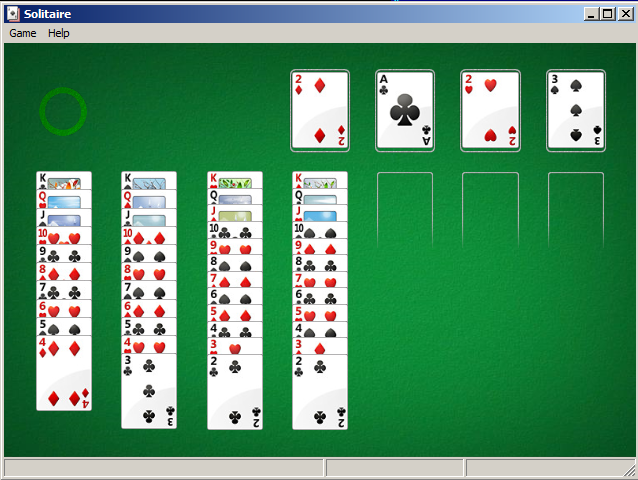
\includegraphics[width=0.6\textwidth]{examples/lines/1.png}
\caption{This is how the game is usually looks like}
\label{fig:lines_1}
\end{figure}

\clearpage
\myindex{\CStandardLibrary!rand()}

So let's see, is it be possible to find the random generator and do some trick with it.
\IDA quickly recognize the standard \TT{\_rand} function in \TT{balltrix.exe} at \TT{0x00403DA0}.
\IDA also shows that it is called only from one place:

\lstinputlisting[style=customasmx86]{examples/lines/random.lst}

We'll call it \q{random}.
Let's not to dive into this function's code yet.

This function is referred from 3 places.

Here are the first two:

\lstinputlisting[style=customasmx86]{examples/lines/1.lst}

Here is the third one:

\lstinputlisting[style=customasmx86]{examples/lines/2.lst}

So the function has only one argument.

10 is passed in first two cases and 5 in third.
We can also notice 
that the board has a size of 10*10 and there are 5 possible colors.
This is it!
The standard \TT{rand()} function returns 
a number in the \TT{0..0x7FFF} range and this is often inconvenient,
so many programmers implement their own random functions which returns a random number in a specified range.
In our case, the range is $0..n-1$ and $n$ is passed as the sole argument of the function.
We can quickly check this in any debugger.

So let's fix the third function call to always return zero.
First, we will replace three instructions (\TT{PUSH/CALL/ADD}) 
by \ac{NOP}s.
Then we'll add \INS{XOR EAX, EAX} instruction, 
to clear the \EAX register.

\lstinputlisting[style=customasmx86]{examples/lines/fixed.lst}

So what we did is we replaced a call to the \TT{random()} 
function by a code which always returns zero.

\clearpage
Let's run it now:

\begin{figure}[H]
\centering
\includegraphics[width=0.6\textwidth]{examples/lines/2.png}
\caption{Practical joke works}
\end{figure}

Oh yes, it works\footnote{Author of this book once did this as a joke for his coworkers with 
the hope that they would stop playing. They didn't.}.

But why are the arguments to the \TT{random()} functions global variables?
That's just because it's possible to change the board size in the game's settings, 
so these values are not hardcoded.
The 10 and 5 values are just defaults.

\mysection{\MinesweeperWinXPExampleChapterName}
\label{minesweeper_winxp}
\myindex{Windows!Windows XP}

For those who are not very good at playing Minesweeper, we could try to reveal the hidden mines in the debugger.

\myindex{\CStandardLibrary!rand()}
\myindex{Windows!PDB}

As we know, Minesweeper places mines randomly, so there has to be some kind of random number generator or
a call to the standard \TT{rand()} C-function.

What is really cool about reversing Microsoft products is that there are \gls{PDB} 
file with symbols (function names, etc).
When we load \TT{winmine.exe} into \IDA, it downloads the 
\gls{PDB} file exactly for this 
executable and shows all names.

So here it is, the only call to \TT{rand()} is this function:

\lstinputlisting[style=customasmx86]{examples/minesweeper/tmp1.lst}

\IDA named it so, and it was the name given to it by Minesweeper's developers.

The function is very simple:

\begin{lstlisting}[style=customc]
int Rnd(int limit)
{
    return rand() % limit;
};
\end{lstlisting}

(There is no \q{limit} name in the \gls{PDB} file; we manually named this argument like this.)

So it returns 
a random value from 0 to a specified limit.

\TT{Rnd()} is called only from one place, 
a function called \TT{StartGame()}, 
and as it seems, this is exactly 
the code which place the mines:

\begin{lstlisting}[style=customasmx86]
.text:010036C7                 push    _xBoxMac
.text:010036CD                 call    _Rnd@4          ; Rnd(x)
.text:010036D2                 push    _yBoxMac
.text:010036D8                 mov     esi, eax
.text:010036DA                 inc     esi
.text:010036DB                 call    _Rnd@4          ; Rnd(x)
.text:010036E0                 inc     eax
.text:010036E1                 mov     ecx, eax
.text:010036E3                 shl     ecx, 5          ; ECX=ECX*32
.text:010036E6                 test    _rgBlk[ecx+esi], 80h
.text:010036EE                 jnz     short loc_10036C7
.text:010036F0                 shl     eax, 5          ; EAX=EAX*32
.text:010036F3                 lea     eax, _rgBlk[eax+esi]
.text:010036FA                 or      byte ptr [eax], 80h
.text:010036FD                 dec     _cBombStart
.text:01003703                 jnz     short loc_10036C7
\end{lstlisting}

Minesweeper allows you to set the board size, so the X (xBoxMac) and Y (yBoxMac) of the board are global variables.
They are passed to \TT{Rnd()} and random 
coordinates are generated.
A mine is placed by the \TT{OR} instruction at \TT{0x010036FA}. 
And if it has been placed before 
(it's possible if the pair of \TT{Rnd()} 
generates a coordinates pair which has been already 
generated), 
then \TT{TEST} and \TT{JNZ} at \TT{0x010036E6} 
jumps to the generation routine again.

\TT{cBombStart} is the global variable containing total number of mines. So this is loop.

The width of the array is 32 
(we can conclude this by looking at the \TT{SHL} instruction, which multiplies one of the coordinates by 32).

The size of the \TT{rgBlk} 
global array can be easily determined by the difference 
between the \TT{rgBlk} 
label in the data segment and the next known one. 
It is 0x360 (864):

\begin{lstlisting}[style=customasmx86]
.data:01005340 _rgBlk          db 360h dup(?)          ; DATA XREF: MainWndProc(x,x,x,x)+574
.data:01005340                                         ; DisplayBlk(x,x)+23
.data:010056A0 _Preferences    dd ?                    ; DATA XREF: FixMenus()+2
...
\end{lstlisting}

$864/32=27$.

So the array size is $27*32$?
It is close to what we know: when we try to set board size to $100*100$ in Minesweeper settings, it fallbacks to a board of size $24*30$.
So this is the maximal board size here.
And the array has a fixed size for any board size.

So let's see all this in \olly.
We will ran Minesweeper, attaching \olly to it and now we can see the memory dump at the address of the \TT{rgBlk} array (\TT{0x01005340})
\footnote{All addresses here are for Minesweeper for Windows XP SP3 English. 
They may differ for other service packs.}.

So we got this memory dump of the array:

\lstinputlisting[style=customasmx86]{examples/minesweeper/1.lst}

\olly, like any other hexadecimal editor, shows 16 bytes per line.
So each 32-byte array row occupies exactly 2 lines here.

This is beginner level (9*9 board).

There is some square 
structure can be seen visually (0x10 bytes).

We will click \q{Run} in \olly to unfreeze the Minesweeper process, then we'll clicked randomly at the Minesweeper window 
and trapped into mine, but now all mines are visible:

\begin{figure}[H]
\centering
\myincludegraphicsSmall{examples/minesweeper/1.png}
\caption{Mines}
\label{fig:minesweeper1}
\end{figure}

By comparing the mine places and the dump, we can conclude that 0x10 stands for border, 0x0F---empty block, 0x8F---mine.
Perhaps, 0x10 is just a \emph{sentinel value}.

Now we'll add comments and also enclose all 0x8F bytes into square brackets:

\lstinputlisting[style=customasmx86]{examples/minesweeper/2.lst}

Now we'll remove all \emph{border bytes} (0x10) and what's beyond those:

\lstinputlisting[style=customasmx86]{examples/minesweeper/3.lst}

Yes, these are mines, now it can be clearly seen and compared with the screenshot.

\clearpage
What is interesting is that we can modify the array right in \olly.
We can remove all mines by changing all 0x8F bytes by 0x0F, and here is what we'll get in Minesweeper:

\begin{figure}[H]
\centering
\myincludegraphicsSmall{examples/minesweeper/3.png}
\caption{All mines are removed in debugger}
\label{fig:minesweeper3}
\end{figure}

We can also move all of them to the first line: 

\begin{figure}[H]
\centering
\myincludegraphicsSmall{examples/minesweeper/2.png}
\caption{Mines set in debugger}
\label{fig:minesweeper2}
\end{figure}

Well, the debugger is not very convenient for eavesdropping (which is our goal anyway), so we'll write a small utility
to dump the contents of the board:

\lstinputlisting[style=customc]{examples/minesweeper/minesweeper_cheater.c}

Just set the \ac{PID}
\footnote{PID it can be seen in Task Manager 
(enable it in \q{View $\rightarrow$ Select Columns})} 
and the address of the array (\TT{0x01005340} for Windows XP SP3 English) 
and it will dump it
\footnote{The compiled executable is here: 
\href{http://beginners.re/examples/minesweeper_WinXP/minesweeper_cheater.exe}{beginners.re}}.

It attaches itself to a win32 process by \ac{PID} and just reads process memory at the address.

\subsection{Finding grid automatically}

This is kind of nuisance to set address each time when we run our utility.
Also, various Minesweeper versions may have the array on different address.
Knowing the fact that there is always a border (0x10 bytes), we can just find it in memory:

\lstinputlisting[style=customc]{examples/minesweeper/cheater2_fragment.c}

Full source code: \url{\RepoURL/examples/minesweeper/minesweeper_cheater2.c}.

\subsection{\Exercises}

\begin{itemize}

\item 
Why do the \emph{border bytes} (or \emph{sentinel values}) (0x10) exist in the array?

What they are for if they are not visible in Minesweeper's interface?
How could it work without them?

\item 
As it turns out, there are more values possible (for open blocks, for flagged by user, etc).
Try to find the meaning of each one.

\item 
Modify my utility so it can remove all mines or set them in a fixed pattern that you want in the Minesweeper
process currently running.

\end{itemize}

\mysection{Hacking Windows clock}

Sometimes I do some kind of first April prank for my coworkers.

Let's find, if we could do something with Windows clock?
Can we force to go clock hands backwards?

First of all, when you click on date/time in status bar,\\
a \emph{C:\textbackslash{}WINDOWS\textbackslash{}SYSTEM32\textbackslash{}TIMEDATE.CPL} module gets executed,
which is usual executable \ac{PE}-file.

Let's see, how it draw hands?
When I open the file (from Windows 7) in Resource Hacker, there are clock faces, but with no hands:

\begin{figure}[H]
\centering
\myincludegraphics{examples/timedate/reshack.png}
\caption{Resource Hacker}
\end{figure}

OK, what we know? How to draw a clock hand? All they are started at the middle of circle, ending with its border.
Hence, we must calculate coordinates of a point on circle's border.
From school-level mathematics we may recall that we have to use sine/cosine functions to draw circle, or at least
square root.
There are no such things in \emph{TIMEDATE.CPL}, at least at first glance.
But, thanks to Microsoft debugging PDB files, I can find a function named \emph{CAnalogClock::DrawHand()}, which calls
\emph{Gdiplus::Graphics::DrawLine()} at least twice.

Here is its code:

\lstinputlisting[style=customasmx86]{examples/timedate/1.lst}

\myindex{Windows!Win32!MulDiv()}
We can see that \emph{DrawLine()} arguments are dependent on result of \emph{MulDiv()} function
and a \emph{table[]} table (name is mine),
which has 8-byte elements (look at \INS{LEA}'s second operand).

What is inside of table[]?

\lstinputlisting[style=customasmx86]{examples/timedate/2.lst}

It's referenced only from \emph{DrawHand()} function.
It has 120 32-bit words or 60 32-bit pairs... wait, 60?
Let's take a closer look at these values.
First of all, I'll zap 6 pairs or 12 32-bit words with zeros, and then I'll put patched \emph{TIMEDATE.CPL}
into \emph{C:\textbackslash{}WINDOWS\textbackslash{}SYSTEM32}.
(You may need to set owner of the *TIMEDATE.CPL* file to your primary user account (instead of \emph{TrustedInstaller}),
and also, boot in safe mode with command prompt so you can copy the file, which is usually locked.)

\begin{figure}[H]
\centering
\includegraphics[width=0.5\textwidth]{examples/timedate/6_pairs_zeroed.png}
\caption{Attempt to run}
\end{figure}

Now when any hand is located at 0..5 seconds/minutes, it's invisible! However, opposite (shorter) part of second hand
is visible and moving.
When any hand is outside of this area, hand is visible as usual.

\myindex{Mathematica}
Let's take even closer look at the table in Mathematica.
I have copypasted table from the \emph{TIMEDATE.CPL} to a \emph{tbl} file (480 bytes).
We will take for granted the fact that these are signed values, because half of elements are below zero (0FFFFE0C1h, etc.).
If these values would be unsigned, they would be suspiciously huge.

\begin{lstlisting}[style=custommath]
In[]:= tbl = BinaryReadList["~/.../tbl", "Integer32"]

Out[]= {0, -7999, 836, -7956, 1663, -7825, 2472, -7608, 3253, -7308, 3999, \
-6928, 4702, -6472, 5353, -5945, 5945, -5353, 6472, -4702, 6928, \
-4000, 7308, -3253, 7608, -2472, 7825, -1663, 7956, -836, 8000, 0, \
7956, 836, 7825, 1663, 7608, 2472, 7308, 3253, 6928, 4000, 6472, \
4702, 5945, 5353, 5353, 5945, 4702, 6472, 3999, 6928, 3253, 7308, \
2472, 7608, 1663, 7825, 836, 7956, 0, 7999, -836, 7956, -1663, 7825, \
-2472, 7608, -3253, 7308, -4000, 6928, -4702, 6472, -5353, 5945, \
-5945, 5353, -6472, 4702, -6928, 3999, -7308, 3253, -7608, 2472, \
-7825, 1663, -7956, 836, -7999, 0, -7956, -836, -7825, -1663, -7608, \
-2472, -7308, -3253, -6928, -4000, -6472, -4702, -5945, -5353, -5353, \
-5945, -4702, -6472, -3999, -6928, -3253, -7308, -2472, -7608, -1663, \
-7825, -836, -7956}

In[]:= Length[tbl]
Out[]= 120
\end{lstlisting}

Let's treat two consecutive 32-bit values as pair:

\begin{lstlisting}[style=custommath]
In[]:= pairs = Partition[tbl, 2]
Out[]= {{0, -7999}, {836, -7956}, {1663, -7825}, {2472, -7608}, \
{3253, -7308}, {3999, -6928}, {4702, -6472}, {5353, -5945}, {5945, \
-5353}, {6472, -4702}, {6928, -4000}, {7308, -3253}, {7608, -2472}, \
{7825, -1663}, {7956, -836}, {8000, 0}, {7956, 836}, {7825, 
1663}, {7608, 2472}, {7308, 3253}, {6928, 4000}, {6472, 
4702}, {5945, 5353}, {5353, 5945}, {4702, 6472}, {3999, 
6928}, {3253, 7308}, {2472, 7608}, {1663, 7825}, {836, 7956}, {0, 
7999}, {-836, 7956}, {-1663, 7825}, {-2472, 7608}, {-3253, 
7308}, {-4000, 6928}, {-4702, 6472}, {-5353, 5945}, {-5945, 
5353}, {-6472, 4702}, {-6928, 3999}, {-7308, 3253}, {-7608, 
2472}, {-7825, 1663}, {-7956, 836}, {-7999, 
0}, {-7956, -836}, {-7825, -1663}, {-7608, -2472}, {-7308, -3253}, \
{-6928, -4000}, {-6472, -4702}, {-5945, -5353}, {-5353, -5945}, \
{-4702, -6472}, {-3999, -6928}, {-3253, -7308}, {-2472, -7608}, \
{-1663, -7825}, {-836, -7956}}

In[]:= Length[pairs]
Out[]= 60
\end{lstlisting}

Let's try to treat each pair as X/Y coordinate and draw all 60 pairs, and also first 15 pairs:

\begin{figure}[H]
\centering
\myincludegraphics{examples/timedate/math.png}
\caption{Mathematica}
\end{figure}

Now this is something!
Each pair is just coordinate.
First 15 pairs are coordinates for $\frac{1}{4}$ of circle.

Perhaps, Microsoft developers precalculated all coordinates and put them into table.
\myindex{Memoization}
This is widespread, though somewhat old school practice -- precalculated table access is faster than calling relatively slow sine/cosine functions\footnote{Today this is known
as \emph{memoization}}.
Sine/cosine operations are not that expensive anymore...

Now I can understand why when I zapped first 6 pairs, hands were invisible at that area: in fact, hands were drawn,
they just had zero length, because hand started at 0:0 coordinate and ended there.

\subsubsection{The prank (practical joke)}

Given all that, how would we force hands to go counterclockwise?
In fact, this is simple, we need just to rotate the table, so each hand, instead of drawing at place of zeroth second,
would be drawing at place of 59th second.

I made the patcher a long time ago, at the very beginning of 2000s, for Windows 2000.
Hard to believe, it still works for Windows 7, perhaps, the table hasn't been changed since then!

The patcher source code: \url{\RepoURL/examples/timedate/time_pt.c}.

Now I can see all hands goes backwards:

\begin{figure}[H]
\centering
\includegraphics[width=0.5\textwidth]{examples/timedate/counterclockwise.png}
\caption{Now it works}
\end{figure}

Well, there is no animation in this book, but if you look closer, you can see, that hands are in fact shows correct
time, but the whole clock face is rotated vertically, like we see it from the inside of clock.

\subsubsection{Windows 2000 leaked source code}

So I did the patcher and then Windows 2000 source code has been leaked (I can't force you to trust me, though).
Let's take a look on source code if that function and table.\\
The file is \emph{win2k/private/shell/cpls/utc/clock.c}:

\begin{lstlisting}[style=customc]
//
//  Array containing the sine and cosine values for hand positions.
//
POINT rCircleTable[] =
{
    { 0,     -7999},
    { 836,   -7956},
    { 1663,  -7825},
    { 2472,  -7608},
    { 3253,  -7308},
...
    { -4702, -6472},
    { -3999, -6928},
    { -3253, -7308},
    { -2472, -7608},
    { -1663, -7825},
    { -836 , -7956},
};

////////////////////////////////////////////////////////////////////////////
//
//  DrawHand
//
//  Draws the hands of the clock.
//
////////////////////////////////////////////////////////////////////////////

void DrawHand(
    HDC hDC,
    int pos,
    HPEN hPen,
    int scale,
    int patMode,
    PCLOCKSTR np)
{
    LPPOINT lppt;
    int radius;

    MoveTo(hDC, np->clockCenter.x, np->clockCenter.y);
    radius = MulDiv(np->clockRadius, scale, 100);
    lppt = rCircleTable + pos;
    SetROP2(hDC, patMode);
    SelectObject(hDC, hPen);

    LineTo( hDC,
            np->clockCenter.x + MulDiv(lppt->x, radius, 8000),
            np->clockCenter.y + MulDiv(lppt->y, radius, 8000) );
}
\end{lstlisting}

Now it's clear: coordinates has been precalculated as if clock face has height and width of $2 \cdot 8000$,
and then it's rescaled to current clock face radius using \emph{MulDiv()} function.

POINT structure\footnote{\url{https://msdn.microsoft.com/en-us/library/windows/desktop/dd162805(v=vs.85).aspx}}
is a structure of two 32-bit values, first is \emph{x}, second is \emph{y}.


\mysection{(Windows 7) Solitaire: practical jokes}

\input{examples/solitaire/51/main_EN}
\input{examples/solitaire/53/main_EN}


\section{FreeCell prank (Windows 7)}

\renewcommand{\CURPATH}{examples/freecell}

This is a prank I once played for my coworkers who played FreeCell solitaire too much.
Can we make FreeCell always deal the same game each time?
Like, you know, in ``Groundhog Day'' movie?

(I'm writing this in November 2019. Somehow, IDA can't get PDBs from Microsoft servers. Maybe Windows 7 is unsupported anymore?
Anyway, I can't get function names...)

\subsection{Part I}

\myindex{\CStandardLibrary!rand()}
\myindex{\CStandardLibrary!srand()}
\myindex{\CStandardLibrary!time()}
So I loaded FreeCell.exe into IDA and found that both rand(), srand() and time() are imported from msvcrt.dll.
time() is indeed used as a seed for srand():

\begin{lstlisting}[style=customasmx86]
.text:01029612                sub_1029612     proc near               ; CODE XREF: sub\_102615C+149
.text:01029612                                                        ; sub\_1029DA6+67
.text:01029612 8B FF                          mov     edi, edi
.text:01029614 56                             push    esi
.text:01029615 57                             push    edi
.text:01029616 6A 00                          push    0               ; Time
.text:01029618 8B F9                          mov     edi, ecx
.text:0102961A FF 15 80 16 00+                call    ds:time
.text:01029620 50                             push    eax             ; Seed
.text:01029621 FF 15 84 16 00+                call    ds:srand
.text:01029627 8B 35 AC 16 00+                mov     esi, ds:rand
.text:0102962D 59                             pop     ecx
.text:0102962E 59                             pop     ecx
.text:0102962F FF D6                          call    esi ; rand
.text:01029631 FF D6                          call    esi ; rand
.text:01029633
.text:01029633                loc_1029633:                            ; CODE XREF: sub\_1029612+26
.text:01029633                                                        ; sub\_1029612+2D
.text:01029633 FF D6                          call    esi ; rand
.text:01029635 83 F8 01                       cmp     eax, 1
.text:01029638 7C F9                          jl      short loc_1029633
.text:0102963A 3D 40 42 0F 00                 cmp     eax, 1000000
.text:0102963F 7F F2                          jg      short loc_1029633
.text:01029641 6A 01                          push    1
.text:01029643 50                             push    eax
.text:01029644 8B CF                          mov     ecx, edi
.text:01029646 E8 2D F8 FF FF                 call    sub_1028E78
.text:0102964B 5F                             pop     edi
.text:0102964C 5E                             pop     esi
.text:0102964D C3                             retn
.text:0102964D                sub_1029612     endp
\end{lstlisting}

Several (redundant) calls to rand() are funny, that reminds me:

``In the morning you will send for a hansom, desiring your man to take neither the first nor the second which may present itself.''
( The Memoirs of Sherlock Holmes, by Arthur Conan Doyle\footnote{\url{http://www.gutenberg.org/files/834/834-0.txt}} )

There is another call of time() and srand() pair, but my \tracer showed that this is the point of our interest:

\begin{lstlisting}
tracer.exe -l:FreeCell.exe bpf=msvcrt.dll!time bpf=msvcrt.dll!srand,args:1

...

TID=5340|(0) msvcrt.dll!time() (called from FreeCell.exe!BASE+0x29620 (0x209620))
TID=5340|(0) msvcrt.dll!time() -> 0x5ddb68aa
TID=5340|(1) msvcrt.dll!srand(0x5ddb68aa) (called from FreeCell.exe!BASE+0x29627 (0x209627))
TID=5340|(1) msvcrt.dll!srand() -> 0x5507e0
TID=5340|(1) msvcrt.dll!srand(0x399f) (called from FreeCell.exe!BASE+0x27d3a (0x207d3a))
TID=5340|(1) msvcrt.dll!srand() -> 0x5507e0
\end{lstlisting}

You see, the time() function returned 0x5ddb68aa and the very same value is used as an argument for srand().

Let's try to force time() to always return 0:

\begin{lstlisting}
tracer.exe -l:FreeCell.exe bpf=msvcrt.dll!time,rt:0 bpf=msvcrt.dll!srand,args:1

...

TID=2104|(0) msvcrt.dll!time() (called from FreeCell.exe!BASE+0x29620 (0xb19620))
TID=2104|(0) msvcrt.dll!time() -> 0x5ddb68f6
TID=2104|(0) Modifying EAX register to 0x0
TID=2104|(1) msvcrt.dll!srand(0x0) (called from FreeCell.exe!BASE+0x29627 (0xb19627))
TID=2104|(1) msvcrt.dll!srand() -> 0x3707e0
TID=2104|(1) msvcrt.dll!srand(0x52f6) (called from FreeCell.exe!BASE+0x27d3a (0xb17d3a))
TID=2104|(1) msvcrt.dll!srand() -> 0x3707e0
\end{lstlisting}

Now I'm seeing the same game each time I'm running FreeCell using \tracer:

\begin{figure}[H]
\centering
\frame{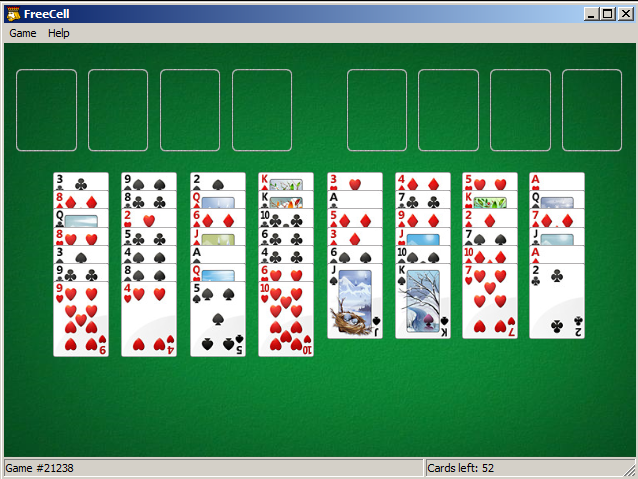
\includegraphics[width=1.0\textwidth]{\CURPATH/freecell1.png}}
\end{figure}

Now how to patch the executable?

We want to pass 0 as an argument to srand() at 0x01029620.
But there is a one-byte instruction: \INS{PUSH EAX}.
\INS{PUSH 0} is two-byte instruction. How to squeeze it into?

What is in other registers at this moment? Using \tracer I'm dumping all them:

\begin{lstlisting}
tracer.exe -l:FreeCell.exe bpx=FreeCell.exe!0x01029620

...

TID=4448|(0) FreeCell.exe!0x1029620
EAX=0x5ddb6ac4 EBX=0x00000000 ECX=0x00000000 EDX=0x00000000
ESI=0x054732d0 EDI=0x054732d0 EBP=0x0020f2bc ESP=0x0020f298
EIP=0x00899620
FLAGS=PF ZF IF
TID=4448|(0) FreeCell.exe!0x1029620
EAX=0x5ddb6ac8 EBX=0x00000002 ECX=0x00000000 EDX=0x00000000
ESI=0xffffff11 EDI=0x054732d0 EBP=0x0020da78 ESP=0x0020d9d4
EIP=0x00899620
FLAGS=PF ZF IF
TID=4448|(0) FreeCell.exe!0x1029620
EAX=0x5ddb6aca EBX=0x00000002 ECX=0x00000000 EDX=0x00000000
ESI=0x7740c460 EDI=0x054732d0 EBP=0x0020da78 ESP=0x0020d9d4
EIP=0x00899620
FLAGS=PF ZF IF
...
\end{lstlisting}

No matter how often I restart the game, ECX and EDX are seems to be always 0.
So I patching \INS{PUSH EAX} at 0x01029620 to \INS{PUSH EDX} (also one-byte instruction),
and now FreeCell always shows the same game to the player.

However, other options could exist.
As a matter of fact, we don't need to pass 0 to srand().
Rather, we want to pass a \emph{constant} to srand() to make game the same each time.
As we can see, EDI's value hasn't been changing. Maybe we could try it as well.

Now a bit harder patching.
Let's open FreeCell.exe in Hiew:

\begin{figure}[H]
\centering
\frame{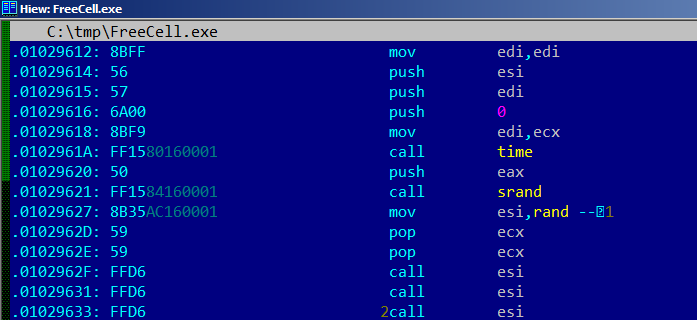
\includegraphics[width=1.0\textwidth]{\CURPATH/hiew1.png}}
\end{figure}

We have no space to replace one-byte \INS{PUSH EAX} with two-byte \INS{PUSH 0}.
\myindex{FIXUP}
And we can't simply fill \verb|CALL ds:time| with \ac{NOP}s, because there is a FIXUP (address of time() function in msvcrt.dll).
(Hiew marked these 4 bytes are gray bytes.)
So what I'm doing: patching first 2 bytes to EB 04. This is a \INS{JMP} to bypass 4 FIXUP-ed bytes:

\begin{figure}[H]
\centering
\frame{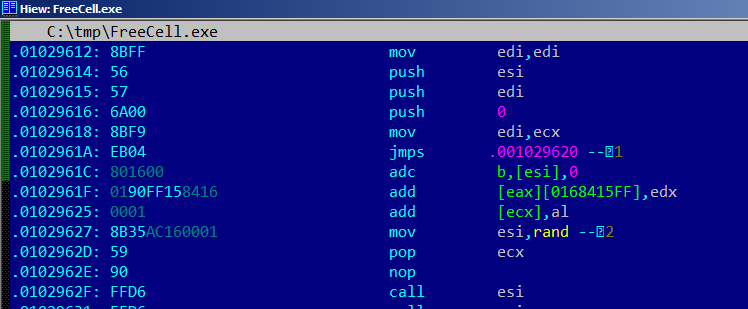
\includegraphics[width=1.0\textwidth]{\CURPATH/hiew2.png}}
\end{figure}

Then I replace \INS{PUSH EAX} with \ac{NOP}. So that srand() would have its zeroes arguments from \INS{PUSH 0} above.
Also, I patch one of \INS{POP ECX} to \ac{NOP}, because I removed one \INS{PUSH}.

\begin{figure}[H]
\centering
\frame{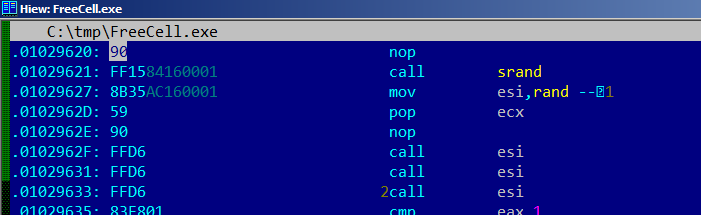
\includegraphics[width=1.0\textwidth]{\CURPATH/hiew3.png}}
\end{figure}

Now Windows loader will write 4-byte FIXUP at 0x0102961C, but we don't care: time()'s address will not be used anymore.

\subsection{Part II: breaking the \emph{Select Game} submenu}

The user can still choose different game in the menu.
Let's see if srand() is still called.
I'm trying to enter 1/2/3 in "Select Game" dialog box:

\begin{lstlisting}
tracer.exe -l:FreeCell.exe bpf=msvcrt.dll!srand,args:1

...

TID=4936|(0) msvcrt.dll!srand(0x5ddb6df9) (called from FreeCell.exe!BASE+0x29627 (0xb49627))
TID=4936|(0) msvcrt.dll!srand() -> 0x5907e0
TID=4936|(0) msvcrt.dll!srand(0x2b40) (called from FreeCell.exe!BASE+0x27d3a (0xb47d3a))
TID=4936|(0) msvcrt.dll!srand() -> 0x5907e0
TID=4936|(0) msvcrt.dll!srand(0x1) (called from FreeCell.exe!BASE+0x27d3a (0xb47d3a))
TID=4936|(0) msvcrt.dll!srand() -> 0x5907e0
TID=4936|(0) msvcrt.dll!srand(0x2) (called from FreeCell.exe!BASE+0x27d3a (0xb47d3a))
TID=4936|(0) msvcrt.dll!srand() -> 0x5907e0
TID=4936|(0) msvcrt.dll!srand(0x3) (called from FreeCell.exe!BASE+0x27d3a (0xb47d3a))
TID=4936|(0) msvcrt.dll!srand() -> 0x5907e0
\end{lstlisting}

Yes, the number user enters is just an argument for srand().
Where it is called?

\begin{lstlisting}
.text:01027CBA                loc_1027CBA:                            ; CODE XREF: sub\_1027AC6+179
.text:01027CBA 83 FF FC                       cmp     edi, 0FFFFFFFCh
.text:01027CBD 75 74                          jnz     short loc_1027D33

...

.text:01027D33                loc_1027D33:                            ; CODE XREF: sub\_1027AC6+1F7
.text:01027D33 57                             push    edi             ; Seed
.text:01027D34 FF 15 84 16 00+                call    ds:srand
.text:01027D3A 59                             pop     ecx
.text:01027D3B 6A 34                          push    34h
.text:01027D3D 5B                             pop     ebx
.text:01027D3E 33 C0                          xor     eax, eax
\end{lstlisting}

I couldn't patch one-byte \INS{PUSH EDI} to two-byte \INS{PUSH 0}.
But I see that there is only one single jump to \verb|loc_1027D33| from the above.

I'm patching \INS{CMP EDI, ...} to \INS{XOR EDI, EDI}, padding the 3rd byte to \ac{NOP}.
I'm patching also JNZ to JMP, so that jump will always occur.

Now FreeCell ignores the number user enters, but suddenly, there is also the same game at start:

\begin{figure}[H]
\centering
\frame{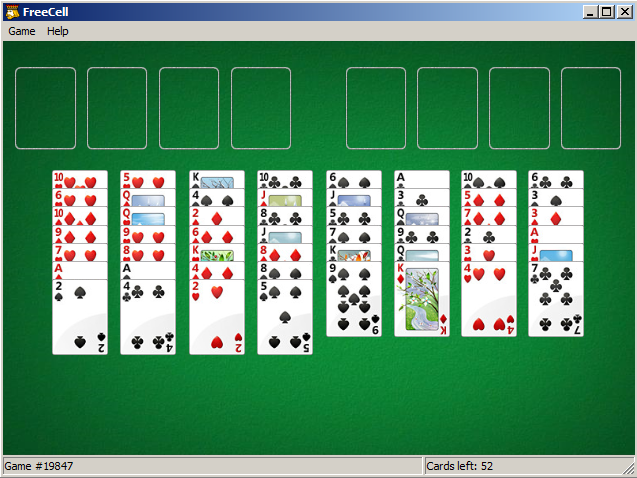
\includegraphics[width=1.0\textwidth]{\CURPATH/freecell2.png}}
\end{figure}

It seems that the code we patched in part I is somehow connected to a code after 0x01027CBD, that executes if EDI==0xFFFFFFFC.
Anyway, our goal is accomplished --- the game is always the same at the start and the user can't choose another using the menu.

\mysection{\RU{Донглы}\EN{Dongles}}
\label{dongles}

% TODO dongle picture

\RU{Автор этих строк иногда делал замену \glslink{dongle}{донглам} или \q{эмуляторы донглов} 
и здесь немного примеров, как это происходит.}
\EN{The author of these lines, occasionally did software copy-protection \gls{dongle} replacements, or \q{dongle emulators} and here
are couple examples of how it's happening.}

\RU{Об одном неописанном здесь случае с Rockey и Z3 вы также можете прочитать здесь}
\EN{About one of the cases about Rocket and Z3 that is not present here, you can read here}:
\url{http://yurichev.com/tmp/SAT_SMT_DRAFT.pdf}.

\EN{\input{examples/dongles/1/main_EN}}
\RU{\input{examples/dongles/1/main_RU}}
\EN{\input{examples/dongles/2/main_EN}}

\RU{\input{examples/dongles/2/main_RU}}
\EN{\input{examples/dongles/3/main_EN}}
\RU{\input{examples/dongles/3/main_RU}}



% I never liked this part:
% \mysection{\q{QR9}: Rubik's cube inspired amateur crypto-algorithm}

Sometimes amateur cryptosystems appear to be pretty bizarre.

The author of this book was once asked to reverse engineer an amateur cryptoalgorithm of some data encryption utility, 
the source code for which was lost\footnote{He also got permission from the customer to publish the algorithm's details}.

Here is the listing exported from \IDA for the original encryption utility:

\lstinputlisting[style=customasmx86]{examples/qr9/qr9_original.lst}

All function and label names were given by me during the analysis.

Let's start from the top. Here is a function that takes two file names and password.

\begin{lstlisting}[style=customasmx86]
.text:00541320 ; int __cdecl crypt_file(char *Str, char *Filename, int password)
.text:00541320 crypt_file      proc near
.text:00541320
.text:00541320 Str             = dword ptr  4
.text:00541320 Filename        = dword ptr  8
.text:00541320 password        = dword ptr  0Ch
.text:00541320
\end{lstlisting}

Open the file and report if an error occurs:

\begin{lstlisting}[style=customasmx86]
.text:00541320                 mov     eax, [esp+Str]
.text:00541324                 push    ebp
.text:00541325                 push    offset Mode     ; "rb"
.text:0054132A                 push    eax             ; Str
.text:0054132B                 call    _fopen          ; open file
.text:00541330                 mov     ebp, eax
.text:00541332                 add     esp, 8
.text:00541335                 test    ebp, ebp
.text:00541337                 jnz     short loc_541348
.text:00541339                 push    offset Format   ; "Cannot open input file!\n"
.text:0054133E                 call    _printf
.text:00541343                 add     esp, 4
.text:00541346                 pop     ebp
.text:00541347                 retn
.text:00541348
.text:00541348 loc_541348:
\end{lstlisting}

\myindex{\CStandardLibrary!fseek()}
\myindex{\CStandardLibrary!ftell()}
Get the file size via \TT{fseek()}/\TT{ftell()}:

\lstinputlisting[style=customasmx86]{examples/qr9/1_EN}

This fragment of code calculates the file size aligned on a 64-byte boundary. 
This is because this cryptographic algorithm works only with 64-byte blocks. 
The operation is pretty straightforward: divide the file size by 64, forget about the remainder and add 1, 
then multiply by 64. 
The following code removes the remainder as if the value has already been divided by 64 and adds 64. 
It is almost the same.

\lstinputlisting[style=customasmx86]{examples/qr9/2_EN}

Allocate buffer with aligned size:

\begin{lstlisting}[style=customasmx86]
.text:00541373                 push    esi             ; Size
.text:00541374                 call    _malloc
\end{lstlisting}

\myindex{\CStandardLibrary!calloc()}
Call memset(), e.g., clear the allocated buffer\footnote{malloc() + memset() could 
be replaced by calloc()}.

\lstinputlisting[style=customasmx86]{examples/qr9/3_EN}

Read file via the standard C function \TT{fread()}.

\begin{lstlisting}[style=customasmx86]
.text:00541392                 mov     eax, [esp+38h+Str]
.text:00541396                 push    eax             ; ElementSize
.text:00541397                 push    ebx             ; DstBuf
.text:00541398                 call    _fread          ; read file
.text:0054139D                 push    ebp             ; File
.text:0054139E                 call    _fclose
\end{lstlisting}

Call \TT{crypt()}. This function takes a buffer, buffer size (aligned) and a password string.

\begin{lstlisting}[style=customasmx86]
.text:005413A3                 mov     ecx, [esp+44h+password]
.text:005413A7                 push    ecx             ; password
.text:005413A8                 push    esi             ; aligned size
.text:005413A9                 push    ebx             ; buffer
.text:005413AA                 call    crypt           ; do crypt
\end{lstlisting}

Create the output file. By the way, the developer forgot to check if it has been created correctly! 
The file opening result is being checked, though.

\begin{lstlisting}[style=customasmx86]
.text:005413AF                 mov     edx, [esp+50h+Filename]
.text:005413B3                 add     esp, 40h
.text:005413B6                 push    offset aWb      ; "wb"
.text:005413BB                 push    edx             ; Filename
.text:005413BC                 call    _fopen
.text:005413C1                 mov     edi, eax
\end{lstlisting}

The newly created file handle is in the \EDI register now. Write signature \q{QR9}.

\begin{lstlisting}[style=customasmx86]
.text:005413C3                 push    edi             ; File
.text:005413C4                 push    1               ; Count
.text:005413C6                 push    3               ; Size
.text:005413C8                 push    offset aQr9     ; "QR9"
.text:005413CD                 call    _fwrite         ; write file signature
\end{lstlisting}

Write the actual file size (not aligned):

\begin{lstlisting}[style=customasmx86]
.text:005413D2                 push    edi             ; File
.text:005413D3                 push    1               ; Count
.text:005413D5                 lea     eax, [esp+30h+Str]
.text:005413D9                 push    4               ; Size
.text:005413DB                 push    eax             ; Str
.text:005413DC                 call    _fwrite         ; write original file size
\end{lstlisting}

Write the encrypted buffer:

\begin{lstlisting}[style=customasmx86]
.text:005413E1                 push    edi             ; File
.text:005413E2                 push    1               ; Count
.text:005413E4                 push    esi             ; Size
.text:005413E5                 push    ebx             ; Str
.text:005413E6                 call    _fwrite         ; write encrypted file
\end{lstlisting}

Close the file and free the allocated buffer:

\begin{lstlisting}[style=customasmx86]
.text:005413EB                 push    edi             ; File
.text:005413EC                 call    _fclose
.text:005413F1                 push    ebx             ; Memory
.text:005413F2                 call    _free
.text:005413F7                 add     esp, 40h
.text:005413FA                 pop     edi
.text:005413FB                 pop     esi
.text:005413FC                 pop     ebx
.text:005413FD                 pop     ebp
.text:005413FE                 retn
.text:005413FE crypt_file      endp
\end{lstlisting}

Here is the reconstructed C code:

\begin{lstlisting}[style=customc]
void crypt_file(char *fin, char* fout, char *pw)
{
	FILE *f;
	int flen, flen_aligned;
	BYTE *buf;

	f=fopen(fin, "rb");
	
	if (f==NULL)
	{
		printf ("Cannot open input file!\n");
		return;
	};

	fseek (f, 0, SEEK_END);
	flen=ftell (f);
	fseek (f, 0, SEEK_SET);

	flen_aligned=(flen&0xFFFFFFC0)+0x40;

	buf=(BYTE*)malloc (flen_aligned);
	memset (buf, 0, flen_aligned);

	fread (buf, flen, 1, f);

	fclose (f);

	crypt (buf, flen_aligned, pw);
	
	f=fopen(fout, "wb");

	fwrite ("QR9", 3, 1, f);
	fwrite (&flen, 4, 1, f);
	fwrite (buf, flen_aligned, 1, f);

	fclose (f);

	free (buf);
};
\end{lstlisting}

The decryption procedure is almost the same:

\begin{lstlisting}[style=customasmx86]
.text:00541400 ; int __cdecl decrypt_file(char *Filename, int, void *Src)
.text:00541400 decrypt_file    proc near
.text:00541400
.text:00541400 Filename        = dword ptr  4
.text:00541400 arg_4           = dword ptr  8
.text:00541400 Src             = dword ptr  0Ch
.text:00541400
.text:00541400                 mov     eax, [esp+Filename]
.text:00541404                 push    ebx
.text:00541405                 push    ebp
.text:00541406                 push    esi
.text:00541407                 push    edi
.text:00541408                 push    offset aRb      ; "rb"
.text:0054140D                 push    eax             ; Filename
.text:0054140E                 call    _fopen
.text:00541413                 mov     esi, eax
.text:00541415                 add     esp, 8
.text:00541418                 test    esi, esi
.text:0054141A                 jnz     short loc_54142E
.text:0054141C                 push    offset aCannotOpenIn_0 ; "Cannot open input file!\n"
.text:00541421                 call    _printf
.text:00541426                 add     esp, 4
.text:00541429                 pop     edi
.text:0054142A                 pop     esi
.text:0054142B                 pop     ebp
.text:0054142C                 pop     ebx
.text:0054142D                 retn
.text:0054142E
.text:0054142E loc_54142E:
.text:0054142E                 push    2               ; Origin
.text:00541430                 push    0               ; Offset
.text:00541432                 push    esi             ; File
.text:00541433                 call    _fseek
.text:00541438                 push    esi             ; File
.text:00541439                 call    _ftell
.text:0054143E                 push    0               ; Origin
.text:00541440                 push    0               ; Offset
.text:00541442                 push    esi             ; File
.text:00541443                 mov     ebp, eax
.text:00541445                 call    _fseek
.text:0054144A                 push    ebp             ; Size
.text:0054144B                 call    _malloc
.text:00541450                 push    esi             ; File
.text:00541451                 mov     ebx, eax
.text:00541453                 push    1               ; Count
.text:00541455                 push    ebp             ; ElementSize
.text:00541456                 push    ebx             ; DstBuf
.text:00541457                 call    _fread
.text:0054145C                 push    esi             ; File
.text:0054145D                 call    _fclose
\end{lstlisting}

Check signature (first 3 bytes):

\begin{lstlisting}[style=customasmx86]
.text:00541462                 add     esp, 34h
.text:00541465                 mov     ecx, 3
.text:0054146A                 mov     edi, offset aQr9_0 ; "QR9"
.text:0054146F                 mov     esi, ebx
.text:00541471                 xor     edx, edx
.text:00541473                 repe cmpsb
.text:00541475                 jz      short loc_541489
\end{lstlisting}

Report an error if the signature is absent:

\begin{lstlisting}[style=customasmx86]
.text:00541477                 push    offset aFileIsNotCrypt ; "File is not encrypted!\n"
.text:0054147C                 call    _printf
.text:00541481                 add     esp, 4
.text:00541484                 pop     edi
.text:00541485                 pop     esi
.text:00541486                 pop     ebp
.text:00541487                 pop     ebx
.text:00541488                 retn
.text:00541489
.text:00541489 loc_541489:
\end{lstlisting}

Call \TT{decrypt()}.

\begin{lstlisting}[style=customasmx86]
.text:00541489                 mov     eax, [esp+10h+Src]
.text:0054148D                 mov     edi, [ebx+3]
.text:00541490                 add     ebp, 0FFFFFFF9h
.text:00541493                 lea     esi, [ebx+7]
.text:00541496                 push    eax             ; Src
.text:00541497                 push    ebp             ; int
.text:00541498                 push    esi             ; int
.text:00541499                 call    decrypt
.text:0054149E                 mov     ecx, [esp+1Ch+arg_4]
.text:005414A2                 push    offset aWb_0    ; "wb"
.text:005414A7                 push    ecx             ; Filename
.text:005414A8                 call    _fopen
.text:005414AD                 mov     ebp, eax
.text:005414AF                 push    ebp             ; File
.text:005414B0                 push    1               ; Count
.text:005414B2                 push    edi             ; Size
.text:005414B3                 push    esi             ; Str
.text:005414B4                 call    _fwrite
.text:005414B9                 push    ebp             ; File
.text:005414BA                 call    _fclose
.text:005414BF                 push    ebx             ; Memory
.text:005414C0                 call    _free
.text:005414C5                 add     esp, 2Ch
.text:005414C8                 pop     edi
.text:005414C9                 pop     esi
.text:005414CA                 pop     ebp
.text:005414CB                 pop     ebx
.text:005414CC                 retn
.text:005414CC decrypt_file    endp
\end{lstlisting}

Here is the reconstructed C code:

\begin{lstlisting}[style=customc]
void decrypt_file(char *fin, char* fout, char *pw)
{
	FILE *f;
	int real_flen, flen;
	BYTE *buf;

	f=fopen(fin, "rb");
	
	if (f==NULL)
	{
		printf ("Cannot open input file!\n");
		return;
	};

	fseek (f, 0, SEEK_END);
	flen=ftell (f);
	fseek (f, 0, SEEK_SET);

	buf=(BYTE*)malloc (flen);

	fread (buf, flen, 1, f);

	fclose (f);

	if (memcmp (buf, "QR9", 3)!=0)
	{
		printf ("File is not encrypted!\n");
		return;
	};

	memcpy (&real_flen, buf+3, 4);

	decrypt (buf+(3+4), flen-(3+4), pw);
	
	f=fopen(fout, "wb");

	fwrite (buf+(3+4), real_flen, 1, f);

	fclose (f);

	free (buf);
};
\end{lstlisting}

OK, now let's go deeper.

Function \TT{crypt()}:

\begin{lstlisting}[style=customasmx86]
.text:00541260 crypt           proc near
.text:00541260
.text:00541260 arg_0           = dword ptr  4
.text:00541260 arg_4           = dword ptr  8
.text:00541260 arg_8           = dword ptr  0Ch
.text:00541260
.text:00541260                 push    ebx
.text:00541261                 mov     ebx, [esp+4+arg_0]
.text:00541265                 push    ebp
.text:00541266                 push    esi
.text:00541267                 push    edi
.text:00541268                 xor     ebp, ebp
.text:0054126A
.text:0054126A loc_54126A:
\end{lstlisting}

\myindex{x86!\Instructions!MOVSD}
This fragment of code copies a part of the input buffer to an internal array we later name \q{cube64}.
The size is in the \ECX register. \TT{MOVSD} stands for \emph{move 32-bit dword}, so, 
16 32-bit dwords are exactly 64 bytes.

\begin{lstlisting}[style=customasmx86]
.text:0054126A                 mov     eax, [esp+10h+arg_8]
.text:0054126E                 mov     ecx, 10h
.text:00541273                 mov     esi, ebx   ; EBX is pointer within input buffer
.text:00541275                 mov     edi, offset cube64
.text:0054127A                 push    1
.text:0054127C                 push    eax
.text:0054127D                 rep movsd
\end{lstlisting}

Call \TT{rotate\_all\_with\_password()}:

\begin{lstlisting}[style=customasmx86]
.text:0054127F                 call    rotate_all_with_password
\end{lstlisting}

Copy encrypted contents back from \q{cube64} to buffer:

\begin{lstlisting}[style=customasmx86]
.text:00541284                 mov     eax, [esp+18h+arg_4]
.text:00541288                 mov     edi, ebx
.text:0054128A                 add     ebp, 40h
.text:0054128D                 add     esp, 8
.text:00541290                 mov     ecx, 10h
.text:00541295                 mov     esi, offset cube64
.text:0054129A                 add     ebx, 40h  ; add 64 to input buffer pointer
.text:0054129D                 cmp     ebp, eax  ; EBP = amount of encrypted data.
.text:0054129F                 rep movsd
\end{lstlisting}

If \EBP is not bigger that the size input argument, then continue to the next block.

\begin{lstlisting}[style=customasmx86]
.text:005412A1                 jl      short loc_54126A
.text:005412A3                 pop     edi
.text:005412A4                 pop     esi
.text:005412A5                 pop     ebp
.text:005412A6                 pop     ebx
.text:005412A7                 retn
.text:005412A7 crypt           endp
\end{lstlisting}

Reconstructed \TT{crypt()} function:

\begin{lstlisting}[style=customc]
void crypt (BYTE *buf, int sz, char *pw)
{
	int i=0;
	
	do
	{
		memcpy (cube, buf+i, 8*8);
		rotate_all (pw, 1);
		memcpy (buf+i, cube, 8*8);
		i+=64;
	}
	while (i<sz);
};
\end{lstlisting}

OK, now let's go deeper in function \TT{rotate\_all\_with\_password()}. 
It takes two arguments: password string and a number.

In \TT{crypt()}, the number 1 is used, and in the \TT{decrypt()} function (where \TT{rotate\_all\_with\_password()} function 
is called too), the number is 3.

\begin{lstlisting}[style=customasmx86]
.text:005411B0 rotate_all_with_password proc near
.text:005411B0
.text:005411B0 arg_0           = dword ptr  4
.text:005411B0 arg_4           = dword ptr  8
.text:005411B0
.text:005411B0                 mov     eax, [esp+arg_0]
.text:005411B4                 push    ebp
.text:005411B5                 mov     ebp, eax
\end{lstlisting}

Check the current character in the password. If it is zero, exit:

\begin{lstlisting}[style=customasmx86]
.text:005411B7                 cmp     byte ptr [eax], 0
.text:005411BA                 jz      exit
.text:005411C0                 push    ebx
.text:005411C1                 mov     ebx, [esp+8+arg_4]
.text:005411C5                 push    esi
.text:005411C6                 push    edi
.text:005411C7
.text:005411C7 loop_begin:
\end{lstlisting}

\myindex{\CStandardLibrary!tolower()}
Call \TT{tolower()}, a standard C function.

\begin{lstlisting}[style=customasmx86]
.text:005411C7                 movsx   eax, byte ptr [ebp+0]
.text:005411CB                 push    eax             ; C
.text:005411CC                 call    _tolower
.text:005411D1                 add     esp, 4
\end{lstlisting}

Hmm, if the password has non-Latin character, it is skipped! 
Indeed, when we run the encryption utility and try non-Latin characters in the password, 
they seem to be ignored.

\begin{lstlisting}[style=customasmx86]
.text:005411D4                 cmp     al, 'a'
.text:005411D6                 jl      short next_character_in_password
.text:005411D8                 cmp     al, 'z'
.text:005411DA                 jg      short next_character_in_password
.text:005411DC                 movsx   ecx, al
\end{lstlisting}

Subtract the value of \q{a} (97) from the character.

\begin{lstlisting}[style=customasmx86]
.text:005411DF                 sub     ecx, 'a'  ; 97
\end{lstlisting}

After subtracting, we'll get 0 for \q{a} here, 1 for \q{b}, etc. And 25 for \q{z}.

\begin{lstlisting}[style=customasmx86]
.text:005411E2                 cmp     ecx, 24
.text:005411E5                 jle     short skip_subtracting
.text:005411E7                 sub     ecx, 24
\end{lstlisting}

It seems, \q{y} and \q{z} are exceptional characters too. 
After that fragment of code, \q{y} becomes 0 and \q{z}~---1. 
This implies that the 26 Latin alphabet symbols become values in the range of 0..23, (24 in total).

\begin{lstlisting}[style=customasmx86]
.text:005411EA
.text:005411EA skip_subtracting:                       ; CODE XREF: rotate_all_with_password+35
\end{lstlisting}

This is actually division via multiplication. 
You can read more about it in the \q{\DivisionByMultSectionName} section~(\myref{sec:divisionbymult}).

The code actually divides the password character's value by 3.
% TODO1: add Mathematica calculations
\begin{lstlisting}[style=customasmx86]
.text:005411EA                 mov     eax, 55555556h
.text:005411EF                 imul    ecx
.text:005411F1                 mov     eax, edx
.text:005411F3                 shr     eax, 1Fh
.text:005411F6                 add     edx, eax
.text:005411F8                 mov     eax, ecx
.text:005411FA                 mov     esi, edx
.text:005411FC                 mov     ecx, 3
.text:00541201                 cdq
.text:00541202                 idiv    ecx
\end{lstlisting}

\EDX is the remainder of the division.

\lstinputlisting[style=customasmx86]{examples/qr9/4_EN}

If the remainder is 2, call \TT{rotate3()}. 
\EDI is the second argument of the \TT{rotate\_all\_with\_password()} function.
As we already noted, 1 is for the encryption operations and 3 is for the decryption. 
So, here is a loop. When encrypting, rotate1/2/3 are to be called the same number of times as 
given in the first argument.

\begin{lstlisting}[style=customasmx86]
.text:00541215 call_rotate3:
.text:00541215                 push    esi
.text:00541216                 call    rotate3
.text:0054121B                 add     esp, 4
.text:0054121E                 dec     edi
.text:0054121F                 jnz     short call_rotate3
.text:00541221                 jmp     short next_character_in_password
.text:00541223
.text:00541223 call_rotate2:
.text:00541223                 test    ebx, ebx
.text:00541225                 jle     short next_character_in_password
.text:00541227                 mov     edi, ebx
.text:00541229
.text:00541229 loc_541229:
.text:00541229                 push    esi
.text:0054122A                 call    rotate2
.text:0054122F                 add     esp, 4
.text:00541232                 dec     edi
.text:00541233                 jnz     short loc_541229
.text:00541235                 jmp     short next_character_in_password
.text:00541237
.text:00541237 call_rotate1:
.text:00541237                 test    ebx, ebx
.text:00541239                 jle     short next_character_in_password
.text:0054123B                 mov     edi, ebx
.text:0054123D
.text:0054123D loc_54123D:
.text:0054123D                 push    esi
.text:0054123E                 call    rotate1
.text:00541243                 add     esp, 4
.text:00541246                 dec     edi
.text:00541247                 jnz     short loc_54123D
.text:00541249
\end{lstlisting}

Fetch the next character from the password string.

\begin{lstlisting}[style=customasmx86]
.text:00541249 next_character_in_password:
.text:00541249                 mov     al, [ebp+1]
\end{lstlisting}

\Gls{increment} the character pointer in the password string:

\begin{lstlisting}[style=customasmx86]
.text:0054124C                 inc     ebp
.text:0054124D                 test    al, al
.text:0054124F                 jnz     loop_begin
.text:00541255                 pop     edi
.text:00541256                 pop     esi
.text:00541257                 pop     ebx
.text:00541258
.text:00541258 exit:
.text:00541258                 pop     ebp
.text:00541259                 retn
.text:00541259 rotate_all_with_password endp
\end{lstlisting}

Here is the reconstructed C code:

\begin{lstlisting}[style=customc]
void rotate_all (char *pwd, int v)
{
	char *p=pwd;

	while (*p)
	{
		char c=*p;
		int q;

		c=tolower (c);

		if (c>='a' && c<='z')
		{
			q=c-'a';
			if (q>24)
				q-=24;

			int quotient=q/3;
			int remainder=q % 3;

			switch (remainder)
			{
			case 0: for (int i=0; i<v; i++) rotate1 (quotient); break;
			case 1: for (int i=0; i<v; i++) rotate2 (quotient); break;
			case 2: for (int i=0; i<v; i++) rotate3 (quotient); break;
			};
		};

		p++;
	};
};
\end{lstlisting}

Now let's go deeper and investigate the rotate1/2/3 functions. 
Each function calls another two functions. 
We eventually will name them \TT{set\_bit()} and \TT{get\_bit()}.

Let's start with \TT{get\_bit()}:

\begin{lstlisting}[style=customasmx86]
.text:00541050 get_bit         proc near
.text:00541050
.text:00541050 arg_0           = dword ptr  4
.text:00541050 arg_4           = dword ptr  8
.text:00541050 arg_8           = byte ptr  0Ch
.text:00541050
.text:00541050                 mov     eax, [esp+arg_4]
.text:00541054                 mov     ecx, [esp+arg_0]
.text:00541058                 mov     al, cube64[eax+ecx*8]
.text:0054105F                 mov     cl, [esp+arg_8]
.text:00541063                 shr     al, cl
.text:00541065                 and     al, 1
.text:00541067                 retn
.text:00541067 get_bit         endp
\end{lstlisting}

\dots in other words: calculate an index in 
the cube64 array: \emph{arg\_4 + arg\_0 * 8}.
Then shift a byte from the array by arg\_8 bits right. 
Isolate the lowest bit and return it.

Let's see another function, \TT{set\_bit()}:

\begin{lstlisting}[style=customasmx86]
.text:00541000 set_bit         proc near
.text:00541000
.text:00541000 arg_0           = dword ptr  4
.text:00541000 arg_4           = dword ptr  8
.text:00541000 arg_8           = dword ptr  0Ch
.text:00541000 arg_C           = byte ptr  10h
.text:00541000
.text:00541000                 mov     al, [esp+arg_C]
.text:00541004                 mov     ecx, [esp+arg_8]
.text:00541008                 push    esi
.text:00541009                 mov     esi, [esp+4+arg_0]
.text:0054100D                 test    al, al
.text:0054100F                 mov     eax, [esp+4+arg_4]
.text:00541013                 mov     dl, 1
.text:00541015                 jz      short loc_54102B
\end{lstlisting}

The value in the \TT{DL} is 1 here. It gets shifted left by arg\_8.
For example, if arg\_8 is 4, the value in the \TT{DL} register is to be 
0x10 or 1000b in binary form.

\begin{lstlisting}[style=customasmx86]
.text:00541017                 shl     dl, cl
.text:00541019                 mov     cl, cube64[eax+esi*8]
\end{lstlisting}

Get a bit from array and explicitly set it. % TODO1: rewrite

\begin{lstlisting}[style=customasmx86]
.text:00541020                 or      cl, dl
\end{lstlisting}

Store it back: % TODO1: rewrite

\begin{lstlisting}[style=customasmx86]
.text:00541022                 mov     cube64[eax+esi*8], cl
.text:00541029                 pop     esi
.text:0054102A                 retn
.text:0054102B
.text:0054102B loc_54102B:
.text:0054102B                 shl     dl, cl
\end{lstlisting}

If arg\_C is not zero\dots

\begin{lstlisting}[style=customasmx86]
.text:0054102D                 mov     cl, cube64[eax+esi*8]
\end{lstlisting}

\myindex{x86!\Instructions!NOT}

\dots invert DL. For example, if DL's state after the shift is 0x10 or 0b1000, 
there is 0xEF to be after the \NOT instruction (or 0b11101111b).

\begin{lstlisting}[style=customasmx86]
.text:00541034                 not     dl
\end{lstlisting}

This instruction clears the bit, in other words, it saves all bits in \TT{CL} which are also set in 
\TT{DL} except those in \TT{DL} which are cleared.
This implies that if \TT{DL} is 11101111b in binary form,
all bits are to be saved except the 5th (counting from lowest bit).

\begin{lstlisting}[style=customasmx86]
.text:00541036                 and     cl, dl
\end{lstlisting}

Store it back:

\begin{lstlisting}[style=customasmx86]
.text:00541038                 mov     cube64[eax+esi*8], cl
.text:0054103F                 pop     esi
.text:00541040                 retn
.text:00541040 set_bit         endp
\end{lstlisting}

It is almost the same as \TT{get\_bit()}, except, if arg\_C is zero, the function clears the specific bit in the array, 
or sets it otherwise.

We also know that the array's size is 64. The first two arguments both in the \TT{set\_bit()} and \TT{get\_bit()} functions
could be seen as 2D coordinates. Then the array is to be an 8*8 matrix.

Here is a C representation of what we know up to now:

\begin{lstlisting}[style=customc]
#define IS_SET(flag, bit)       ((flag) & (bit))
#define SET_BIT(var, bit)       ((var) |= (bit))
#define REMOVE_BIT(var, bit)    ((var) &= ~(bit))

static BYTE cube[8][8];

void set_bit (int x, int y, int shift, int bit)
{
	if (bit)
		SET_BIT (cube[x][y], 1<<shift);
	else
		REMOVE_BIT (cube[x][y], 1<<shift);
};

bool get_bit (int x, int y, int shift)
{
	if ((cube[x][y]>>shift)&1==1)
		return 1;
	return 0;
};
\end{lstlisting}

Now let's get back to the rotate1/2/3 functions.

\begin{lstlisting}[style=customasmx86]
.text:00541070 rotate1         proc near
.text:00541070
\end{lstlisting}

Internal array allocation in the local stack, with size of 64 bytes:

\begin{lstlisting}[style=customasmx86]
.text:00541070 internal_array_64= byte ptr -40h
.text:00541070 arg_0           = dword ptr  4
.text:00541070
.text:00541070                 sub     esp, 40h
.text:00541073                 push    ebx
.text:00541074                 push    ebp
.text:00541075                 mov     ebp, [esp+48h+arg_0]
.text:00541079                 push    esi
.text:0054107A                 push    edi
.text:0054107B                 xor     edi, edi        ; EDI is loop1 counter
\end{lstlisting}

\EBX is a pointer to the internal array:

\begin{lstlisting}[style=customasmx86]
.text:0054107D                 lea     ebx, [esp+50h+internal_array_64]
.text:00541081
\end{lstlisting}

Here we have two nested loops:

\lstinputlisting[style=customasmx86]{examples/qr9/5_EN}

\dots we see that both loops' counters are in the range of 0..7. 
Also they are used as the first and second argument for the \TT{get\_bit()} function.
The third argument to \TT{get\_bit()} is the only argument of \TT{rotate1()}. 
The return value from \TT{get\_bit()} is placed in the internal array.

Prepare a pointer to the internal array again:

\lstinputlisting[style=customasmx86]{examples/qr9/6_EN}

\dots this code is placing the contents of the internal array to the cube global array via the \TT{set\_bit()} function, 
\emph{but} in a different order!
Now the counter of the first loop is in the range of 7 to 0, \glslink{decrement}{decrementing} at each iteration!

The C code representation looks like:

\begin{lstlisting}[style=customc]
void rotate1 (int v)
{
	bool tmp[8][8]; // internal array
	int i, j;

	for (i=0; i<8; i++)
		for (j=0; j<8; j++)
			tmp[i][j]=get_bit (i, j, v);

	for (i=0; i<8; i++)
		for (j=0; j<8; j++)
			set_bit (j, 7-i, v, tmp[x][y]);
};
\end{lstlisting}

Not very understandable, but if we take a look at \TT{rotate2()} function:

\lstinputlisting[style=customasmx86]{examples/qr9/7_EN}

It is \emph{almost} the same, except the order of the arguments of the \TT{get\_bit()} and \TT{set\_bit()} is different. 
Let's rewrite it in C-like code:

\begin{lstlisting}[style=customc]
void rotate2 (int v)
{
	bool tmp[8][8]; // internal array
	int i, j;

	for (i=0; i<8; i++)
		for (j=0; j<8; j++)
			tmp[i][j]=get_bit (v, i, j);

	for (i=0; i<8; i++)
		for (j=0; j<8; j++)
			set_bit (v, j, 7-i, tmp[i][j]);
};
\end{lstlisting}

Let's also rewrite the \TT{rotate3()} function:

\begin{lstlisting}[style=customc]
void rotate3 (int v)
{
	bool tmp[8][8];
	int i, j;

	for (i=0; i<8; i++)
		for (j=0; j<8; j++)
			tmp[i][j]=get_bit (i, v, j);

	for (i=0; i<8; i++)
		for (j=0; j<8; j++)
			set_bit (7-j, v, i, tmp[i][j]);
};
\end{lstlisting}

Well, now things are simpler. If we consider cube64 as a 3D cube of size 8*8*8, where each element is a bit, 
\TT{get\_bit()} and \TT{set\_bit()} take just the coordinates of a bit as input.

The rotate1/2/3 functions are in fact rotating all bits in a specific plane. 
These three functions are one for each cube side and the \TT{v} argument sets the plane in the range of 0..7.

Maybe the algorithm's author was thinking of a 8*8*8 Rubik's cube
\footnote{\href{http://en.wikipedia.org/wiki/Rubik's_Cube}{wikipedia}}?!

Yes, indeed.

Let's look closer into the \TT{decrypt()} function, here is its rewritten version:

\begin{lstlisting}[style=customc]
void decrypt (BYTE *buf, int sz, char *pw)
{
	char *p=strdup (pw);
	strrev (p);
	int i=0;

	do
	{
		memcpy (cube, buf+i, 8*8);
		rotate_all (p, 3);
		memcpy (buf+i, cube, 8*8);
		i+=64;
	}
	while (i<sz);
	
	free (p);
};
\end{lstlisting}

It is almost the same as for \TT{crypt()}, \emph{but} the password string is reversed by the
strrev() \footnote{\href{http://msdn.microsoft.com/en-us/library/9hby7w40(VS.80).aspx}{MSDN}}
standard C function and \TT{rotate\_all()} is called with argument 3. 

This implies that in case of decryption, each corresponding rotate1/2/3 call is to be performed thrice.

This is almost as in Rubik'c cube! 
If you want to get back, do the same in reverse order and direction! 
If you want to undo the effect of rotating one place in clockwise direction, 
rotate it once in counter-clockwise direction, or thrice in clockwise direction.

\TT{rotate1()} is apparently for rotating the \q{front} plane. 
\TT{rotate2()} is apparently for rotating the \q{top} plane. 
\TT{rotate3()} is apparently for rotating the \q{left} plane.

Let's get back to the core of the \TT{rotate\_all()} function:

\begin{lstlisting}[style=customc]
q=c-'a';
if (q>24)
	q-=24;

int quotient=q/3; // in range 0..7
int remainder=q % 3;

switch (remainder)
{
    case 0: for (int i=0; i<v; i++) rotate1 (quotient); break; // front
    case 1: for (int i=0; i<v; i++) rotate2 (quotient); break; // top
    case 2: for (int i=0; i<v; i++) rotate3 (quotient); break; // left
};
\end{lstlisting}

Now it is much simpler to understand: each password character defines a side (one of three) and a plane (one of 8). 
3*8 = 24, that is why two the last two characters of the Latin alphabet are remapped to fit an alphabet of exactly 
24 elements.

The algorithm is clearly weak: in case of short passwords you can see
that in the encrypted file there are 
the original bytes of the original file in a binary file editor.

Here is the whole source code reconstructed:

\lstinputlisting[style=customc]{examples/qr9/qr9.cpp}



% TODO translate
% TODO: OpenSSL tool, URLs, etc
\mysection{Encrypted database case \#1}
\label{encrypted_DB1}

(This part has been first appeared in my blog at 26-Aug-2015.
Some discussion: \url{https://news.ycombinator.com/item?id=10128684}.)

\subsection{Base64 and entropy}

\myindex{XML}
I've got the \ac{XML} file containing some encrypted data.
Perhaps, it's related to some orders and/or customers information.

\begin{lstlisting}
<?xml version = "1.0" encoding = "UTF-8"?>
<Orders>
	<Order>
		<OrderID>1</OrderID>
		<Data>yjmxhXUbhB/5MV45chPsXZWAJwIh1S0aD9lFn3XuJMSxJ3/E+UE3hsnH</Data>
	</Order>
	<Order>
		<OrderID>2</OrderID>
		<Data>0KGe/wnypFBjsy+U0C2P9fC5nDZP3XDZLMPCRaiBw9OjIk6Tu5U=</Data>
	</Order>
	<Order>
		<OrderID>3</OrderID>
		<Data>mqkXfdzvQKvEArdzh+zD9oETVGBFvcTBLs2ph1b5bYddExzp</Data>
	</Order>
	<Order>
		<OrderID>4</OrderID>
		<Data>FCx6JhIDqnESyT3HAepyE1BJ3cJd7wCk+APCRUeuNtZdpCvQ2MR/7kLXtfUHuA==</Data>
	</Order>
...
\end{lstlisting}

The file is available \href{https://raw.githubusercontent.com/DennisYurichev/RE-for-beginners/master/examples/encrypted_DB1/encrypted.xml}{here}.

\myindex{base64}
This is clearly base64-encoded data, because all strings consisting of Latin characters, digits,
plus (+) and slash (/) symbols.
There can be 1 or 2 padding symbols (=), but they are never occurred in the middle of string.
Keeping in mind these base64 properties, it's very easy to recognize them.

Let's decode them and calculate entropies (\myref{entropy}) of these blocks in Wolfram Mathematica:

\begin{lstlisting}
In[]:= ListOfBase64Strings =
  Map[First[#[[3]]] &, Cases[Import["encrypted.xml"], XMLElement["Data", _, _], Infinity]];

In[]:= BinaryStrings =
  Map[ImportString[#, {"Base64", "String"}] &, ListOfBase64Strings];

In[]:= Entropies = Map[N[Entropy[2, #]] &, BinaryStrings];

In[]:= Variance[Entropies]
Out[]= 0.0238614
\end{lstlisting}

\myindex{Variance}
Variance is low.
This means the entropy values are not very different from each other.
This is visible on graph:

\begin{lstlisting}
In[]:= ListPlot[Entropies]
\end{lstlisting}

\begin{figure}[H]
\centering
\myincludegraphics{examples/encrypted_DB1/entropy.png}
\end{figure}

Most values are between 5.0 and 5.4.
This is a sign that the data is compressed and/or encrypted.

To understand variance, let's calculate entropies of all lines in Conan Doyle's \emph{The Hound of the Baskervilles} book:

\begin{lstlisting}
In[]:= BaskervillesLines = Import["http://www.gutenberg.org/cache/epub/2852/pg2852.txt", "List"];

In[]:= EntropiesT = Map[N[Entropy[2, #]] &, BaskervillesLines];

In[]:= Variance[EntropiesT]
Out[]= 2.73883

In[]:= ListPlot[EntropiesT]
\end{lstlisting}

\begin{figure}[H]
\centering
\myincludegraphics{examples/encrypted_DB1/conan_doyle.png}
\end{figure}

Most values are gathered around value of 4, but there are also values which are smaller,
and they are influenced final variance value.

Perhaps, shortest strings has smaller entropy, let's take short string from the Conan Doyle's book:

\begin{lstlisting}
In[]:= Entropy[2, "Yes, sir."] // N
Out[]= 2.9477
\end{lstlisting}

Let's try even shorter:

\begin{lstlisting}
In[]:= Entropy[2, "Yes"] // N
Out[]= 1.58496

In[]:= Entropy[2, "No"] // N
Out[]= 1.
\end{lstlisting}

\subsection{Is data compressed?}

OK, so our data is compressed and/or encrypted.
Is it compressed? Almost all data compressors put some header at the start, signature, or something like that.
As we can see, there are no consistent data at the start of each block.
It's still possible that this is a handmade data compressor, but they are very rare.
On the other hand, handmade cryptoalgorithms are much more popular, because it's very easy to make it work.
\myindex{memfrob()}
\myindex{ROT13}
Even primitive keyless cryptosystems like \emph{memfrob()}\footnote{\url{http://linux.die.net/man/3/memfrob}}
and ROT13 works fine without errors.
It's a serious challenge to write data compressor from scratch using only fantasy and imagination in a way so it will have no evident bugs.
Some programmers implements data compression functions by reading textbooks, but this is also rare.
The most popular two ways are:
\myindex{zlib}
1) just take open-source library like zlib;
2) copy\&paste something from somewhere.
Open-source data compressions algorithms usually puts some kind of header, and so do
algorithms from sites like \url{http://www.codeproject.com/}.

\subsection{Is data encrypted?}

Major data encryption algorithms process data in blocks. DES---8 bytes, AES---16 bytes.
If the input buffer is not divided evenly by block size, it's padded by zeroes (or something else),
so encrypted data will be aligned by cryptoalgorithm's block size.
This is not our case.

Using Wolfram Mathematica, I analyzed block's lengths:

\begin{lstlisting}
In[]:= Counts[Map[StringLength[#] &, BinaryStrings]]
Out[]= <|42 -> 1858, 38 -> 1235, 36 -> 699, 46 -> 1151, 40 -> 1784,
 44 -> 1558, 50 -> 366, 34 -> 291, 32 -> 74, 56 -> 15, 48 -> 716,
 30 -> 13, 52 -> 156, 54 -> 71, 60 -> 3, 58 -> 6, 28 -> 4|>
\end{lstlisting}

1858 blocks has size of 42 bytes, 1235 blocks has size of 38 bytes, etc.

I made a graph:

\begin{lstlisting}
ListPlot[Counts[Map[StringLength[#] &, BinaryStrings]]]
\end{lstlisting}

\begin{figure}[H]
\centering
\myincludegraphics{examples/encrypted_DB1/lengths.png}
\end{figure}

So, most blocks has size between $\textasciitilde{}36$ and $\textasciitilde{}48$.
There is also another thing to notice: all block sizes are even.
No single block with odd size.

There are, however, stream ciphers which can operate on byte level or even on bit level.

\subsection{CryptoPP}
\myindex{CryptoPP}

The program which can browse this encrypted database is written C\# and the .NET code
is heavily obfuscated.
Nevertheless, there is DLL with x86 code, which, after brief examination,
has parts of the CryptoPP popular open-source library!
(I just spotted \q{CryptoPP} strings inside.)
Now it's very easy to find all functions inside of DLL because CryptoPP library is open-source.

\myindex{AES}
CryptoPP library has a lot of crypto-functions, including AES (AKA Rijndael).
Newer x86 CPUs has AES helper instructions like \INS{AESENC}, \INS{AESDEC} and \INS{AESKEYGENASSIST}
\footnote{\url{https://en.wikipedia.org/wiki/AES_instruction_set}}.
They are not performing encryption/decryption completely, but they do significant amount of job.
And newer CryptoPP versions use them.
For example, here:
\href{https://github.com/mmoss/cryptopp/blob/2772f7b57182b31a41659b48d5f35a7b6cedd34d/src/rijndael.cpp#L1034}{1},
\href{https://github.com/mmoss/cryptopp/blob/2772f7b57182b31a41659b48d5f35a7b6cedd34d/src/rijndael.cpp#L1000}{2}.
\myindex{x86!\Instructions!AESENC}
\myindex{x86!\Instructions!AESDEC}
\myindex{tracer}
To my surprise, during decryption, \INS{AESENC} gets executed, while \INS{AESDEC} is not
(I just checked with my tracer utility, but any debugger can be used).
I checked, if my CPU really supports AES instructions. Some Intel i3 CPUs are not.
And if not, CryptoPP library falling back to AES functions implemented in old way
\footnote{\url{https://github.com/mmoss/cryptopp/blob/2772f7b57182b31a41659b48d5f35a7b6cedd34d/src/rijndael.cpp#L355}}.
But my CPU supports them.
Why \INS{AESDEC} is still not executed?
Why the program use AES encryption in order to decrypt database?

OK, it's not a problem to find a function which encrypts block.
It is called \\
\emph{CryptoPP::Rijndael::Enc::ProcessAndXorBlock}:
\href{https://github.com/mmoss/cryptopp/blob/2772f7b57182b31a41659b48d5f35a7b6cedd34d/src/rijndael.cpp#L349}{src},
and it can call another function: \\
\emph{Rijndael::Enc::AdvancedProcessBlocks()}
\href{https://github.com/mmoss/cryptopp/blob/2772f7b57182b31a41659b48d5f35a7b6cedd34d/src/rijndael.cpp#L1179}{src},
which, in turn, can call two other functions (
\href{https://github.com/mmoss/cryptopp/blob/2772f7b57182b31a41659b48d5f35a7b6cedd34d/src/rijndael.cpp#L1000}{AESNI\_Enc\_Block}
and
\href{https://github.com/mmoss/cryptopp/blob/2772f7b57182b31a41659b48d5f35a7b6cedd34d/src/rijndael.cpp#L1012}{AESNI\_Enc\_4\_Blocks}
)
which has \INS{AESENC} instructions.

So, judging by CryptoPP internals, \\
\emph{CryptoPP::Rijndael::Enc::ProcessAndXorBlock()} encrypts one 16-byte block.
Let's set breakpoint on it and see, what happens during decryption.
I use my simple tracer tool again.
The software must decrypt first data block now.
Oh, by the way, here is the first data block converted from base64 encoding to hexadecimal data,
let's have it at hand:

\lstinputlisting{examples/encrypted_DB1/1.lst}

These are also arguments of the function from CryptoPP source files:

\begin{lstlisting}
size_t Rijndael::Enc::AdvancedProcessBlocks(const byte *inBlocks, const byte *xorBlocks, byte *outBlocks, size_t length, word32 flags);
\end{lstlisting}

So it has 5 arguments. Possible flags are:

\begin{lstlisting}
enum {BT_InBlockIsCounter=1, BT_DontIncrementInOutPointers=2, BT_XorInput=4, BT_ReverseDirection=8, BT_AllowParallel=16} FlagsForAdvancedProcessBlocks;
\end{lstlisting}

OK, run tracer on \emph{ProcessAndXorBlock()} function:

\lstinputlisting{examples/encrypted_DB1/2.lst}

Here we can see inputs to the \emph{ProcessAndXorBlock()} function, and outputs from it.

This is output from the function during first call:

\begin{lstlisting}
00000000: C7 39 4E 7B 33 1B D6 1F-B8 31 10 39 39 13 A5 5D ".9N{3....1.99..]"
\end{lstlisting}

Then the \emph{ProcessAndXorBlock()} is called with zero-length block, but with 8 flag (\emph{BT\_ReverseDirection}).

Second call:

\begin{lstlisting}
00000000: 45 00 20 00 4A 00 4F 00-48 00 4E 00 53 00 00 00 "E. .J.O.H.N.S..."
\end{lstlisting}

Wow, there is some string familiar to us!

Third call:

\begin{lstlisting}
00000000: B1 27 7F E4 9F 01 E3 81-CF C6 12 FB B9 7C F1 BC ".'...........|.."
\end{lstlisting}

The first output is very similar to the first 16 bytes of the encrypted buffer.

Output of the first call of \emph{ProcessAndXorBlock()}:

\begin{lstlisting}
00000000: C7 39 4E 7B 33 1B D6 1F-B8 31 10 39 39 13 A5 5D ".9N{3....1.99..]"
\end{lstlisting}

First 16 bytes of encrypted buffer:

\begin{lstlisting}
00000000: CA 39 B1 85 75 1B 84 1F F9 31 5E 39 72 13 EC 5D  .9..u....1^9r..]
\end{lstlisting}

There are too much equal bytes!
How come AES encryption result can be very similar to the encrypted buffer while this is not
encryption but rather decryption?!

\subsection{Cipher Feedback mode}

\myindex{Cipher Feedback mode}
\myindex{XOR}
The answer is \ac{CFB}:
in this mode, AES algorithm used not as encryption algorithm, but as a device which generates cryptographically secure random data.
The actual encryption is happening using simple XOR operation.

Here is encryption algorithm (images are taken from Wikipedia):

\begin{figure}[H]
\centering
\myincludegraphics{examples/encrypted_DB1/601px-CFB_encryption.png}
\end{figure}

And decryption:

\begin{figure}[H]
\centering
\myincludegraphics{examples/encrypted_DB1/601px-CFB_decryption.png}
\label{fig:CFB_decryption}
\end{figure}

Now let's see: AES encryption operation generates 16 bytes (or 128 bits) of \emph{random} data
to be used while XOR-ing, who forces us to use all 16 bytes?
If at the last iteration we've got 1 byte of data, let's xor 1 byte of data with 1 byte of generated
\emph{random} data?
This leads to important property of \ac{CFB} mode: data can be not padded, data of arbitrary size
can be encrypted and decrypted.

Oh, that's why all encrypted blocks are not padded.
And that's why \INS{AESDEC} instruction is never called.

Let's try to decrypt first block manually, using Python.
\ac{CFB} mode also use \ac{IV}, as a \emph{seed} for \ac{CSPRNG}.
In our case, \ac{IV} is the block which is encrypted at first iteration:

\begin{lstlisting}
0038B920: 01 00 00 00 FF FF FF FF-79 C1 69 0B 67 C1 04 7D "........y.i.g..}"
\end{lstlisting}

Oh, and we also have to recover encryption key.
\myindex{x86!\Instructions!AESKEYGENASSIST}
There is \INS{AESKEYGENASSIST} is DLL, and it is called, and it is used in the \\
\emph{Rijndael::Base::UncheckedSetKey()} function:
\href{https://github.com/mmoss/cryptopp/blob/2772f7b57182b31a41659b48d5f35a7b6cedd34d/src/rijndael.cpp#L198}{src}.
It's easy to find it in IDA and set breakpoint. Let's see:

\begin{lstlisting}
... tracer.exe -l:filename.exe bpf=filename.exe!0x435c30,args:3,dump_args:0x10

Warning: no tracer.cfg file.
PID=2068|New process software.exe
no module registered with image base 0x77320000
no module registered with image base 0x76e20000
no module registered with image base 0x77320000
no module registered with image base 0x77220000
Warning: unknown (to us) INT3 breakpoint at ntdll.dll!LdrVerifyImageMatchesChecksum+0x96c (0x776c103b)
(0) software.exe!0x435c30(0x15e8000, 0x10, 0x14f808) (called from software.exe!.text+0x22fa1 (0x13d3fa1))
Argument 1/3
015E8000: CD C5 7E AD 28 5F 6D E1-CE 8F CC 29 B1 21 88 8E "..~.(_m....).!.."
Argument 3/3
0014F808: 38 82 58 01 C8 B9 46 00-01 D1 3C 01 00 F8 14 00 "8.X...F...<....."
Argument 3/3 +0x0: software.exe!.rdata+0x5238
Argument 3/3 +0x8: software.exe!.text+0x1c101
(0) software.exe!0x435c30() -> 0x13c2801
PID=2068|Process software.exe exited. ExitCode=0 (0x0)
\end{lstlisting}

So this is the key: \emph{CD C5 7E AD 28 5F 6D E1-CE 8F CC 29 B1 21 88 8E}.

During manual decryption we've got this:

\begin{lstlisting}
00000000: 0D 00 FF FE 46 00 52 00  41 00 4E 00 4B 00 49 00  ....F.R.A.N.K.I.
00000010: 45 00 20 00 4A 00 4F 00  48 00 4E 00 53 00 66 66  E. .J.O.H.N.S.ff
00000020: 66 66 66 9E 61 40 D4 07  06 01                    fff.a@....
\end{lstlisting}

Now this is something readable!
And now we can see why there were so many equal bytes at the first decryption iteration:
because plaintext has so many zero bytes!

Let's decrypt the second block:

\begin{lstlisting}
00000000: 17 98 D0 84 3A E9 72 4F  DB 82 3F AD E9 3E 2A A8  ....:.rO..?..>*.
00000010: 41 00 52 00 52 00 4F 00  4E 00 CD CC CC CC CC CC  A.R.R.O.N.......
00000020: 1B 40 D4 07 06 01                                 .@....
\end{lstlisting}

Third, fourth and fifth:

\begin{lstlisting}
00000000: 5D 90 59 06 EF F4 96 B4  7C 33 A7 4A BE FF 66 AB  ].Y.....|3.J..f.
00000010: 49 00 47 00 47 00 53 00  00 00 00 00 00 C0 65 40  I.G.G.S.......e@
00000020: D4 07 06 01                                       ....
\end{lstlisting}

\begin{lstlisting}
00000000: D3 15 34 5D 21 18 7C 6E  AA F8 2D FE 38 F9 D7 4E  ..4]!.|n..-.8..N
00000010: 41 00 20 00 44 00 4F 00  48 00 45 00 52 00 54 00  A. .D.O.H.E.R.T.
00000020: 59 00 48 E1 7A 14 AE FF  68 40 D4 07 06 02        Y.H.z...h@....
\end{lstlisting}

\begin{lstlisting}
00000000: 1E 8B 90 0A 17 7B C5 52  31 6C 4E 2F DE 1B 27 19  .....{.R1lN...'.
00000010: 41 00 52 00 43 00 55 00  53 00 00 00 00 00 00 60  A.R.C.U.S.......
00000020: 66 40 D4 07 06 03                                 f@....
\end{lstlisting}

All blocks decrypted seems correct except of first 16 bytes part.

\subsection{Initializing Vector}

What can affect first 16 bytes?

Let's back to \ac{CFB} decryption algorithm again: \myref{fig:CFB_decryption}.

We can see that \ac{IV} can affect to first block decryption operation, but not the second,
because during the second iteration, ciphertext from the first iteration is used, and in case of decryption,
it's the same, no matter what \ac{IV} has!

So probably, \ac{IV} is different each time.
Using my tracer, I'll take a look at the first input during decryption of the second block
of \ac{XML} file:

\begin{lstlisting}
0038B920: 02 00 00 00 FE FF FF FF-79 C1 69 0B 67 C1 04 7D "........y.i.g..}"
\end{lstlisting}

\dots third:

\begin{lstlisting}
0038B920: 03 00 00 00 FD FF FF FF-79 C1 69 0B 67 C1 04 7D "........y.i.g..}"
\end{lstlisting}

It seems, first and fifth byte are changed each time.
I finally concluded that the first 32-bit integer is just OrderID from the \ac{XML} file,
and the second 32-bit integer is also OrderID, but negated. All other 8 bytes are same for each operation.
Now I have decrypted the whole database:
\url{https://raw.githubusercontent.com/DennisYurichev/RE-for-beginners/master/examples/encrypted_DB1/decrypted.full.txt}.

The Python script used for this is:
\url{https://github.com/DennisYurichev/RE-for-beginners/blob/master/examples/encrypted_DB1/decrypt_blocks.py}.

Perhaps, the author wanted each block encrypted differently, so he/she used OrderID as part of key.
It would be also possible to make different AES key instead of \ac{IV}.

So now we know that \ac{IV} only affects first block during decryption in \ac{CFB} mode, this is
feature of it.
All other blocks can be decrypted without knowledge \ac{IV}, but using the key.

OK, so why \ac{CFB} mode? Apparently, because the very first AES example on CryptoPP wiki
uses \ac{CFB} mode:
\url{http://www.cryptopp.com/wiki/Advanced_Encryption_Standard#Encrypting_and_Decrypting_Using_AES}.
Supposedly, developer choose it for simplicity:
the example can encrypt/decrypt text strings with arbitrary lengths, without padding.

It is very likely, program's author(s) just copypasted the example from CryptoPP wiki page.
Many programmers do so.

The only difference that \ac{IV} is chosen randomly in CryptoPP wiki example, while this indeterminism
wasn't allowable to programmers of the software we are dissecting now,
so they choose to initialize \ac{IV} using Order ID.

Now we can proceed to analyzing matter of each byte in the decrypted block.

\subsection{Structure of the buffer}

Let's take first four decrypted blocks:

\begin{lstlisting}
00000000: 0D 00 FF FE 46 00 52 00  41 00 4E 00 4B 00 49 00  ....F.R.A.N.K.I.
00000010: 45 00 20 00 4A 00 4F 00  48 00 4E 00 53 00 66 66  E. .J.O.H.N.S.ff
00000020: 66 66 66 9E 61 40 D4 07  06 01                    fff.a@....

00000000: 0B 00 FF FE 4C 00 4F 00  52 00 49 00 20 00 42 00  ....L.O.R.I. .B.
00000010: 41 00 52 00 52 00 4F 00  4E 00 CD CC CC CC CC CC  A.R.R.O.N.......
00000020: 1B 40 D4 07 06 01                                 .@....

00000000: 0A 00 FF FE 47 00 41 00  52 00 59 00 20 00 42 00  ....G.A.R.Y. .B.
00000010: 49 00 47 00 47 00 53 00  00 00 00 00 00 C0 65 40  I.G.G.S.......e@
00000020: D4 07 06 01                                       ....

00000000: 0F 00 FF FE 4D 00 45 00  4C 00 49 00 4E 00 44 00  ....M.E.L.I.N.D.
00000010: 41 00 20 00 44 00 4F 00  48 00 45 00 52 00 54 00  A. .D.O.H.E.R.T.
00000020: 59 00 48 E1 7A 14 AE FF  68 40 D4 07 06 02        Y.H.z...h@....
\end{lstlisting}

UTF-16 encoded text strings are clearly visible, these are names and surnames.
The first byte (or 16-bit word) is seems string length, we can visually check it.
\emph{FF FE} is seems Unicode \ac{BOM}.

There are 12 more bytes after each string.

Using this script
(\url{https://github.com/DennisYurichev/RE-for-beginners/blob/master/examples/encrypted_DB1/dump_buffer_rest.py})
I've got random selection of the \emph{tails}:

\lstinputlisting{examples/encrypted_DB1/tails.lst}

We first see the 0x40 and 0x07 bytes present in each \emph{tail}.
The very last byte s always in 1..0x1F (1..31) range, I've checked.
The penultimate byte is always in 1..0xC (1..12) range.
Wow, that looks like a date!
Year can be represented as 16-bit value, and maybe last 4 bytes is date (16 bits for year, 8 bits
for month and 8 more for day)?
0x7DD is 2013, 0x7D5 is 2005, etc. Seems fine. This is a date.
There are 8 more bytes.
Judging by the fact this is database named \emph{orders}, maybe some kind of sum is present here?
I made attempt to interpret it as double-precision IEEE 754 floating point and dump all values!

Some are:

\begin{lstlisting}
71.0
134.0
51.95
53.0
121.99
96.95
98.95
15.95
85.95
184.99
94.95
29.95
85.0
36.0
130.99
115.95
87.99
127.95
114.0
150.95
\end{lstlisting}

Looks like real!

Now we can dump names, sums and dates.

\begin{lstlisting}
plain:
00000000: 0D 00 FF FE 46 00 52 00  41 00 4E 00 4B 00 49 00  ....F.R.A.N.K.I.
00000010: 45 00 20 00 4A 00 4F 00  48 00 4E 00 53 00 66 66  E. .J.O.H.N.S.ff
00000020: 66 66 66 9E 61 40 D4 07  06 01                    fff.a@....
OrderID= 1 name= FRANKIE JOHNS sum= 140.95 date= 2004 / 6 / 1

plain:
00000000: 0B 00 FF FE 4C 00 4F 00  52 00 49 00 20 00 42 00  ....L.O.R.I. .B.
00000010: 41 00 52 00 52 00 4F 00  4E 00 CD CC CC CC CC CC  A.R.R.O.N.......
00000020: 1B 40 D4 07 06 01                                 .@....
OrderID= 2 name= LORI BARRON sum= 6.95 date= 2004 / 6 / 1

plain:
00000000: 0A 00 FF FE 47 00 41 00  52 00 59 00 20 00 42 00  ....G.A.R.Y. .B.
00000010: 49 00 47 00 47 00 53 00  00 00 00 00 00 C0 65 40  I.G.G.S.......e@
00000020: D4 07 06 01                                       ....
OrderID= 3 name= GARY BIGGS sum= 174.0 date= 2004 / 6 / 1

plain:
00000000: 0F 00 FF FE 4D 00 45 00  4C 00 49 00 4E 00 44 00  ....M.E.L.I.N.D.
00000010: 41 00 20 00 44 00 4F 00  48 00 45 00 52 00 54 00  A. .D.O.H.E.R.T.
00000020: 59 00 48 E1 7A 14 AE FF  68 40 D4 07 06 02        Y.H.z...h@....
OrderID= 4 name= MELINDA DOHERTY sum= 199.99 date= 2004 / 6 / 2

plain:
00000000: 0B 00 FF FE 4C 00 45 00  4E 00 41 00 20 00 4D 00  ....L.E.N.A. .M.
00000010: 41 00 52 00 43 00 55 00  53 00 00 00 00 00 00 60  A.R.C.U.S.......
00000020: 66 40 D4 07 06 03                                 f@....
OrderID= 5 name= LENA MARCUS sum= 179.0 date= 2004 / 6 / 3
\end{lstlisting}

See more: \url{https://raw.githubusercontent.com/DennisYurichev/RE-for-beginners/master/examples/encrypted_DB1/decrypted.full.with_data.txt}.
Or filtered: \url{https://github.com/DennisYurichev/RE-for-beginners/blob/master/examples/encrypted_DB1/decrypted.short.txt}.
Seems correct.

This is some kind of \ac{OOP} serialization, i.e., packing differently typed values into binary buffer for storing and/or transmitting.

\subsection{Noise at the end}

The only question remaining is that sometimes, \emph{tail} is bigger:

\begin{lstlisting}
00000000: 0E 00 FF FE 54 00 48 00  45 00 52 00 45 00 53 00  ....T.H.E.R.E.S.
00000010: 45 00 20 00 54 00 55 00  54 00 54 00 4C 00 45 00  E. .T.U.T.T.L.E.
00000020: 66 66 66 66 66 1E 63 40  D4 07 07 1A 00 07 07 19  fffff.c@........
OrderID= 172 name= THERESE TUTTLE sum= 152.95 date= 2004 / 7 / 26
\end{lstlisting}

(\emph{00 07 07 19} bytes are not used and is ballast.)

\begin{lstlisting}
00000000: 0C 00 FF FE 4D 00 45 00  4C 00 41 00 4E 00 49 00  ....M.E.L.A.N.I.
00000010: 45 00 20 00 4B 00 49 00  52 00 4B 00 00 00 00 00  E. .K.I.R.K.....
00000020: 00 20 64 40 D4 07 09 02  00 02                    . d@......
OrderID= 286 name= MELANIE KIRK sum= 161.0 date= 2004 / 9 / 2
\end{lstlisting}

(\emph{00 02} are not used.)

After close examination, we can see, that the noise at the end of \emph{tail} is just left
from previous encryption!

Here are two subsequent buffers:

\begin{lstlisting}
00000000: 10 00 FF FE 42 00 4F 00  4E 00 4E 00 49 00 45 00  ....B.O.N.N.I.E.
00000010: 20 00 47 00 4F 00 4C 00  44 00 53 00 54 00 45 00   .G.O.L.D.S.T.E.
00000020: 49 00 4E 00 9A 99 99 99  99 79 46 40 D4 07 07 19  I.N......yF@....
OrderID= 171 name= BONNIE GOLDSTEIN sum= 44.95 date= 2004 / 7 / 25

00000000: 0E 00 FF FE 54 00 48 00  45 00 52 00 45 00 53 00  ....T.H.E.R.E.S.
00000010: 45 00 20 00 54 00 55 00  54 00 54 00 4C 00 45 00  E. .T.U.T.T.L.E.
00000020: 66 66 66 66 66 1E 63 40  D4 07 07 1A 00 07 07 19  fffff.c@........
OrderID= 172 name= THERESE TUTTLE sum= 152.95 date= 2004 / 7 / 26
\end{lstlisting}

(The last \emph{07 07 19} bytes are copied from the previous plaintext buffer.)

Another two subsequent buffers:

\begin{lstlisting}
00000000: 0D 00 FF FE 4C 00 4F 00  52 00 45 00 4E 00 45 00  ....L.O.R.E.N.E.
00000010: 20 00 4F 00 54 00 4F 00  4F 00 4C 00 45 00 CD CC   .O.T.O.O.L.E...
00000020: CC CC CC 3C 5E 40 D4 07  09 02                    ...<^@....
OrderID= 285 name= LORENE OTOOLE sum= 120.95 date= 2004 / 9 / 2

00000000: 0C 00 FF FE 4D 00 45 00  4C 00 41 00 4E 00 49 00  ....M.E.L.A.N.I.
00000010: 45 00 20 00 4B 00 49 00  52 00 4B 00 00 00 00 00  E. .K.I.R.K.....
00000020: 00 20 64 40 D4 07 09 02  00 02                    . d@......
OrderID= 286 name= MELANIE KIRK sum= 161.0 date= 2004 / 9 / 2
\end{lstlisting}

The last 02 byte has been copied from the previous plaintext buffer.

It's possible if the buffer used while encrypting is global and/or isn't clearing before
each encryption.
The final buffer size is also chaotic, nevertheless, the bug left uncaught
because it doesn't affect decrypting process, which just ignores noise at the end.
This is common mistake.
\myindex{OpenSSL}
\myindex{Heartbleed}
It's been present in OpenSSL (Heartbleed bug).

\subsection{Conclusion}

Summary:
every practicing reverse engineer should be familiar with major crypto algorithms and
also major cryptographical modes.
Some books about it: \myref{crypto_books}.

\emph{Encrypted} database contents has been artificially constructed by me for the sake of demonstration.
I've got most popular USA names and surnames from there: \url{http://stackoverflow.com/questions/1803628/raw-list-of-person-names},
and combined them randomly.
Dates and sums were also generated randomly.

All files used in this part are here: \url{https://github.com/DennisYurichev/RE-for-beginners/tree/master/examples/encrypted_DB1}.

Nevertheless, many features like these I've observed in real-world software applications.
This example is based on them.

\subsection{Post Scriptum: brute-forcing \ac{IV}}

The case you have just seen has been artificially constructed, but is based on a real application I've reverse engineered.
When I've been working on it, I first noticed that \ac{IV} has been generating using some 32-bit number,
and I wasn't able to find a link between this value and OrderID.
So I prepared to use brute-force, which is indeed possible here.

It's not a problem to enumerate all 32-bit values and try each as a base for \ac{IV}.
Then you decrypt the first 16-byte block and check for zero bytes, which are always at fixed places.

\mysection{Overclocking Cointerra Bitcoin miner}
\myindex{Bitcoin}
\myindex{BeagleBone}

There was Cointerra Bitcoin miner, looking like that:

\begin{figure}[H]
\centering
\myincludegraphics{examples/bitcoin_miner/board.jpg}
\caption{Board}
\end{figure}

And there was also (possibly leaked) utility\footnote{Can be downloaded here: \url{\RepoURL/examples/bitcoin_miner/files/cointool-overclock}}
which can set clock rate for the board.
It runs on additional BeagleBone Linux ARM board (small board at bottom of the picture).

And the author was once asked, is it possible to hack this utility to see, which frequency can be set and which are not.
And it is possible to tweak it?

The utility must be executed like that: \TT{./cointool-overclock 0 0 900}, where 900 is frequency in MHz.
If the frequency is too high, utility will print \q{Error with arguments} and exit.

This is a fragment of code around reference to \q{Error with arguments} text string:

\begin{lstlisting}[style=customasmARM]

...

.text:0000ABC4         STR      R3, [R11,#var_28]
.text:0000ABC8         MOV      R3, #optind
.text:0000ABD0         LDR      R3, [R3]
.text:0000ABD4         ADD      R3, R3, #1
.text:0000ABD8         MOV      R3, R3,LSL#2
.text:0000ABDC         LDR      R2, [R11,#argv]
.text:0000ABE0         ADD      R3, R2, R3
.text:0000ABE4         LDR      R3, [R3]
.text:0000ABE8         MOV      R0, R3  ; nptr
.text:0000ABEC         MOV      R1, #0  ; endptr
.text:0000ABF0         MOV      R2, #0  ; base
.text:0000ABF4         BL       strtoll
.text:0000ABF8         MOV      R2, R0
.text:0000ABFC         MOV      R3, R1
.text:0000AC00         MOV      R3, R2
.text:0000AC04         STR      R3, [R11,#var_2C]
.text:0000AC08         MOV      R3, #optind
.text:0000AC10         LDR      R3, [R3]
.text:0000AC14         ADD      R3, R3, #2
.text:0000AC18         MOV      R3, R3,LSL#2
.text:0000AC1C         LDR      R2, [R11,#argv]
.text:0000AC20         ADD      R3, R2, R3
.text:0000AC24         LDR      R3, [R3]
.text:0000AC28         MOV      R0, R3  ; nptr
.text:0000AC2C         MOV      R1, #0  ; endptr
.text:0000AC30         MOV      R2, #0  ; base
.text:0000AC34         BL       strtoll
.text:0000AC38         MOV      R2, R0
.text:0000AC3C         MOV      R3, R1
.text:0000AC40         MOV      R3, R2
.text:0000AC44         STR      R3, [R11,#third_argument]
.text:0000AC48         LDR      R3, [R11,#var_28]
.text:0000AC4C         CMP      R3, #0
.text:0000AC50         BLT      errors_with_arguments
.text:0000AC54         LDR      R3, [R11,#var_28]
.text:0000AC58         CMP      R3, #1
.text:0000AC5C         BGT      errors_with_arguments
.text:0000AC60         LDR      R3, [R11,#var_2C]
.text:0000AC64         CMP      R3, #0
.text:0000AC68         BLT      errors_with_arguments
.text:0000AC6C         LDR      R3, [R11,#var_2C]
.text:0000AC70         CMP      R3, #3
.text:0000AC74         BGT      errors_with_arguments
.text:0000AC78         LDR      R3, [R11,#third_argument]
.text:0000AC7C         CMP      R3, #0x31
.text:0000AC80         BLE      errors_with_arguments
.text:0000AC84         LDR      R2, [R11,#third_argument]
.text:0000AC88         MOV      R3, #950
.text:0000AC8C         CMP      R2, R3
.text:0000AC90         BGT      errors_with_arguments
.text:0000AC94         LDR      R2, [R11,#third_argument]
.text:0000AC98         MOV      R3, #0x51EB851F
.text:0000ACA0         SMULL    R1, R3, R3, R2
.text:0000ACA4         MOV      R1, R3,ASR#4
.text:0000ACA8         MOV      R3, R2,ASR#31
.text:0000ACAC         RSB      R3, R3, R1
.text:0000ACB0         MOV      R1, #50
.text:0000ACB4         MUL      R3, R1, R3
.text:0000ACB8         RSB      R3, R3, R2
.text:0000ACBC         CMP      R3, #0
.text:0000ACC0         BEQ      loc_ACEC
.text:0000ACC4
.text:0000ACC4 errors_with_arguments
.text:0000ACC4                                         
.text:0000ACC4         LDR      R3, [R11,#argv]
.text:0000ACC8         LDR      R3, [R3]
.text:0000ACCC         MOV      R0, R3  ; path
.text:0000ACD0         BL       __xpg_basename
.text:0000ACD4         MOV      R3, R0
.text:0000ACD8         MOV      R0, #aSErrorWithArgu ; format
.text:0000ACE0         MOV      R1, R3
.text:0000ACE4         BL       printf
.text:0000ACE8         B        loc_ADD4
.text:0000ACEC ; ------------------------------------------------------------
.text:0000ACEC
.text:0000ACEC loc_ACEC                 ; CODE XREF: main+66C
.text:0000ACEC         LDR      R2, [R11,#third_argument]
.text:0000ACF0         MOV      R3, #499
.text:0000ACF4         CMP      R2, R3
.text:0000ACF8         BGT      loc_AD08
.text:0000ACFC         MOV      R3, #0x64
.text:0000AD00         STR      R3, [R11,#unk_constant]
.text:0000AD04         B        jump_to_write_power
.text:0000AD08 ; ------------------------------------------------------------
.text:0000AD08
.text:0000AD08 loc_AD08                 ; CODE XREF: main+6A4
.text:0000AD08         LDR      R2, [R11,#third_argument]
.text:0000AD0C         MOV      R3, #799
.text:0000AD10         CMP      R2, R3
.text:0000AD14         BGT      loc_AD24
.text:0000AD18         MOV      R3, #0x5F
.text:0000AD1C         STR      R3, [R11,#unk_constant]
.text:0000AD20         B        jump_to_write_power
.text:0000AD24 ; ------------------------------------------------------------
.text:0000AD24
.text:0000AD24 loc_AD24                 ; CODE XREF: main+6C0
.text:0000AD24         LDR      R2, [R11,#third_argument]
.text:0000AD28         MOV      R3, #899
.text:0000AD2C         CMP      R2, R3
.text:0000AD30         BGT      loc_AD40
.text:0000AD34         MOV      R3, #0x5A
.text:0000AD38         STR      R3, [R11,#unk_constant]
.text:0000AD3C         B        jump_to_write_power
.text:0000AD40 ; ------------------------------------------------------------
.text:0000AD40
.text:0000AD40 loc_AD40                 ; CODE XREF: main+6DC
.text:0000AD40         LDR      R2, [R11,#third_argument]
.text:0000AD44         MOV      R3, #999
.text:0000AD48         CMP      R2, R3
.text:0000AD4C         BGT      loc_AD5C
.text:0000AD50         MOV      R3, #0x55
.text:0000AD54         STR      R3, [R11,#unk_constant]
.text:0000AD58         B        jump_to_write_power
.text:0000AD5C ; ------------------------------------------------------------
.text:0000AD5C
.text:0000AD5C loc_AD5C                 ; CODE XREF: main+6F8
.text:0000AD5C         LDR      R2, [R11,#third_argument]
.text:0000AD60         MOV      R3, #1099
.text:0000AD64         CMP      R2, R3
.text:0000AD68         BGT      jump_to_write_power
.text:0000AD6C         MOV      R3, #0x50
.text:0000AD70         STR      R3, [R11,#unk_constant]
.text:0000AD74
.text:0000AD74 jump_to_write_power                     ; CODE XREF: main+6B0
.text:0000AD74                                         ; main+6CC ...
.text:0000AD74         LDR      R3, [R11,#var_28]
.text:0000AD78         UXTB     R1, R3
.text:0000AD7C         LDR      R3, [R11,#var_2C]
.text:0000AD80         UXTB     R2, R3
.text:0000AD84         LDR      R3, [R11,#unk_constant]
.text:0000AD88         UXTB     R3, R3
.text:0000AD8C         LDR      R0, [R11,#third_argument]
.text:0000AD90         UXTH     R0, R0
.text:0000AD94         STR      R0, [SP,#0x44+var_44]
.text:0000AD98         LDR      R0, [R11,#var_24]
.text:0000AD9C         BL       write_power
.text:0000ADA0         LDR      R0, [R11,#var_24]
.text:0000ADA4         MOV      R1, #0x5A
.text:0000ADA8         BL       read_loop
.text:0000ADAC         B        loc_ADD4

...

.rodata:0000B378 aSErrorWithArgu DCB "%s: Error with arguments",0xA,0 ; DATA XREF: main+684

...

\end{lstlisting}

Function names were present in debugging information of the original binary, like \TT{write\_power}, \TT{read\_loop}.
But labels inside functions were named by me.

\myindex{UNIX!getopt}
\myindex{strtoll()}
\TT{optind} name looks familiar. It is from \emph{getopt} *NIX library intended for command-line parsing---well,
this is exactly what happens inside.
Then, the 3rd argument (where frequency value is to be passed) is converted from a string to a number using
a call to \emph{strtoll()} function.

The value is then checked against various constants.
At 0xACEC, it's checked, if it is lesser or equal to 499, and if it is so,
0x64 is to be passed to \TT{write\_power()} function (which sends a command through USB using \TT{send\_msg()}).
If it is greater than 499, jump to 0xAD08 is occurred.

At 0xAD08 it's checked, if it's lesser or equal to 799. 0x5F is then passed to \TT{write\_power()} function in case of success.

There are more checks: for 899 at 0xAD24, for 0x999 at 0xAD40 and finally, for 1099 at 0xAD5C.
If the input frequency is lesser or equal to 1099, 0x50 will be passed (at 0xAD6C) to \TT{write\_power()} function.
And there is some kind of bug.
If the value is still greater than 1099, the value itself is passed into \TT{write\_power()} function.
Oh, it's not a bug, because we can't get here: value is checked first against 950 at 0xAC88, and if it is greater, error message will be displayed and the utility will finish.

Now the table between frequency in MHz and value passed to \TT{write\_power()} function:

\begin{center}
\begin{longtable}{ | l | l | l | }
\hline
\HeaderColor MHz & \HeaderColor hexadecimal & \HeaderColor decimal \\
\hline
499MHz & 0x64 & 100 \\
\hline
799MHz & 0x5f & 95 \\
\hline
899MHz & 0x5a & 90 \\
\hline
999MHz & 0x55 & 85 \\
\hline
1099MHz & 0x50 & 80 \\
\hline
\end{longtable}
\end{center}

As it seems, a value passed to the board is gradually decreasing during frequency increasing.

Now we see that value of 950MHz is a hardcoded limit, at least in this utility. Can we trick it?

Let's back to this piece of code:

\begin{lstlisting}[style=customasmARM]
.text:0000AC84      LDR     R2, [R11,#third_argument]
.text:0000AC88      MOV     R3, #950
.text:0000AC8C      CMP     R2, R3
.text:0000AC90      BGT     errors_with_arguments ; I've patched here to 00 00 00 00
\end{lstlisting}

We must disable \INS{BGT} branch instruction at 0xAC90 somehow. And this is ARM in ARM mode, because, as we see, all addresses are increasing by 4, i.e., each instruction has size of 4 bytes.
\TT{NOP} (no operation) instruction in ARM mode is just four zero bytes: \TT{00 00 00 00}.
So by writing four zeros at 0xAC90 address (or physical offset in file 0x2C90) we can disable the check.

Now it's possible to set frequencies up to 1050MHz. Even more is possible, but due to the bug, if input value is greater than 1099, a value \emph{as is} in MHz will be passed to the board, which is incorrect.

I didn't go further, but if I had to, I would try to decrease a value which is passed to \TT{write\_power()} function.

Now the scary piece of code which I skipped at first:

\lstinputlisting[style=customasmARM]{examples/bitcoin_miner/tmp1.lst}

Division via multiplication is used here, and constant is 0x51EB851F.
I wrote a simple programmer's calculator\footnote{\ProgCalcURL} for myself.
And I have there a feature to calculate modulo inverse.

\begin{lstlisting}
modinv32(0x51EB851F)
Warning, result is not integer: 3.125000
(unsigned) dec: 3 hex: 0x3 bin: 11
\end{lstlisting}

That means that \INS{SMULL} instruction at 0xACA0 is basically divides 3rd argument by 3.125.
In fact, all \TT{modinv32()} function in my calculator does, is this:

\[
\frac{1}{\frac{input}{2^{32}}} = \frac{2^{32}}{input}
\]

Then there are additional shifts and now we see than 3rg argument is just divided by 50.
And then it's multiplied by 50 again.
Why?
This is simplest check, if the input value is can be divided by 50 evenly.
If the value of this expression is non-zero, $x$ can't be divided by 50 evenly:

\[
x-((\frac{x}{50}) \cdot 50)
\]

This is in fact simple way to calculate remainder of division.

And then, if the remainder is non-zero, error message is displayed.
So this utility takes frequency values in form like 850, 900, 950, 1000, etc., but not 855 or 911.

That's it! If you do something like that, please be warned that you may damage your board, just as in case of overclocking other devices like \ac{CPU}s, \ac{GPU}s, etc.
If you have a Cointerra board, do this on your own risk!


% TODO translate
\mysection{Breaking simple executable cryptor}

I've got an executable file which is encrypted by relatively simple encryption.
\href{\GitHubBlobMasterURL/examples/simple_exec_crypto/files/cipher.bin}{Here is it} (only executable section is left here).

First, all encryption function does is just adds number of position in buffer to the byte.
Here is how this can be encoded in Python:

\begin{lstlisting}[caption=Python script,style=custompy]
#!/usr/bin/env python
def e(i, k):
    return chr ((ord(i)+k) % 256)

def encrypt(buf):
    return e(buf[0], 0)+ e(buf[1], 1)+ e(buf[2], 2) + e(buf[3], 3)+ e(buf[4], 4)+ e(buf[5], 5)+ e(buf[6], 6)+ e(buf[7], 7)+
           e(buf[8], 8)+ e(buf[9], 9)+ e(buf[10], 10)+ e(buf[11], 11)+ e(buf[12], 12)+ e(buf[13], 13)+ e(buf[14], 14)+ e(buf[15], 15)
\end{lstlisting}

Hence, if you encrypt buffer with 16 zeros, you'll get \emph{0, 1, 2, 3 ... 12, 13, 14, 15}.

\myindex{Propagating Cipher Block Chaining}
Propagating Cipher Block Chaining (PCBC) is also used, here is how it works:

\begin{figure}[H]
\centering
\myincludegraphics{examples/simple_exec_crypto/601px-PCBC_encryption.png}
\caption{Propagating Cipher Block Chaining encryption (image is taken from Wikipedia article)}
\end{figure}

The problem is that it's too boring to recover IV (Initialization Vector) each time.
Brute-force is also not an option, because IV is too long (16 bytes).
Let's see, if it's possible to recover IV for arbitrary encrypted executable file?

Let's try simple frequency analysis.
This is 32-bit x86 executable code, so let's gather statistics about most frequent bytes and opcodes.
I tried huge oracle.exe file from Oracle RDBMS version 11.2 for windows x86 and I've found that the most frequent byte (no surprise) is zero (~10\%).
The next most frequent byte is (again, no surprise) 0xFF (~5\%).
The next is 0x8B (~5\%).

\myindex{x86!\Instructions!MOV}
0x8B is opcode for \INS{MOV}, this is indeed one of the most busy x86 instructions.
Now what about popularity of zero byte?
If compiler needs to encode value bigger than 127, it has to use 32-bit displacement instead of 8-bit one, but large values are very rare,
so it is padded by zeros.
\myindex{x86!\Instructions!LEA}
\myindex{x86!\Instructions!PUSH}
\myindex{x86!\Instructions!CALL}
This is at least in \INS{LEA}, \INS{MOV}, \INS{PUSH}, \INS{CALL}.

For example:

\begin{lstlisting}[style=customasmx86]
8D B0 28 01 00 00                 lea     esi, [eax+128h]
8D BF 40 38 00 00                 lea     edi, [edi+3840h]
\end{lstlisting}

Displacements bigger than 127 are very popular, but they are rarely exceeds 0x10000
(indeed, such large memory buffers/structures are also rare).

Same story with \INS{MOV}, large constants are rare, the most heavily used are 0, 1, 10, 100, $2^n$, and so on.
Compiler has to pad small constants by zeros to represent them as 32-bit values:

\begin{lstlisting}[style=customasmx86]
BF 02 00 00 00                    mov     edi, 2
BF 01 00 00 00                    mov     edi, 1
\end{lstlisting}

Now about 00 and FF bytes combined: jumps (including conditional) and calls can pass execution flow forward or backwards, but very often,
within the limits of the current executable module.
If forward, displacement is not very big and also padded with zeros.
If backwards, displacement is represented as negative value, so padded with FF bytes.
For example, transfer execution flow forward:

\begin{lstlisting}[style=customasmx86]
E8 43 0C 00 00                    call    _function1
E8 5C 00 00 00                    call    _function2
0F 84 F0 0A 00 00                 jz      loc_4F09A0
0F 84 EB 00 00 00                 jz      loc_4EFBB8
\end{lstlisting}

Backwards:

\begin{lstlisting}[style=customasmx86]
E8 79 0C FE FF                    call    _function1
E8 F4 16 FF FF                    call    _function2
0F 84 F8 FB FF FF                 jz      loc_8212BC
0F 84 06 FD FF FF                 jz      loc_FF1E7D
\end{lstlisting}

FF byte is also very often occurred in negative displacements like these:

\begin{lstlisting}[style=customasmx86]
8D 85 1E FF FF FF                 lea     eax, [ebp-0E2h]
8D 95 F8 5C FF FF                 lea     edx, [ebp-0A308h]
\end{lstlisting}

So far so good. Now we have to try various 16-byte keys, decrypt executable section and measure how often 00, FF and 8B bytes are occurred.
Let's also keep in sight how PCBC decryption works:

\begin{figure}[H]
\centering
\myincludegraphics{examples/simple_exec_crypto/640px-PCBC_decryption.png}
\caption{Propagating Cipher Block Chaining decryption (image is taken from Wikipedia article)}
\end{figure}

The good news is that we don't really have to decrypt whole piece of data, but only slice by slice, this is exactly how I did in my previous example: \myref{XOR_mask_2}.

Now I'm trying all possible bytes (0..255) for each byte in key and just pick the byte producing maximal amount of 00/FF/8B bytes in a decrypted slice:

\begin{lstlisting}[style=custompy]
#!/usr/bin/env python
import sys, hexdump, array, string, operator

KEY_LEN=16

def chunks(l, n):
    # split n by l-byte chunks
    # https://stackoverflow.com/q/312443
    n = max(1, n)
    return [l[i:i + n] for i in range(0, len(l), n)]

def read_file(fname):
    file=open(fname, mode='rb')
    content=file.read()
    file.close()
    return content

def decrypt_byte (c, key):
    return chr((ord(c)-key) % 256)

def XOR_PCBC_step (IV, buf, k):
    prev=IV
    rt=""
    for c in buf:
	new_c=decrypt_byte(c, k)
        plain=chr(ord(new_c)^ord(prev))
	prev=chr(ord(c)^ord(plain))
	rt=rt+plain
    return rt

each_Nth_byte=[""]*KEY_LEN

content=read_file(sys.argv[1])
# split input by 16-byte chunks:
all_chunks=chunks(content, KEY_LEN)
for c in all_chunks:
    for i in range(KEY_LEN):
        each_Nth_byte[i]=each_Nth_byte[i] + c[i]

# try each byte of key
for N in range(KEY_LEN):
    print "N=", N
    stat={}
    for i in range(256):
        tmp_key=chr(i)
	tmp=XOR_PCBC_step(tmp_key,each_Nth_byte[N], N)
        # count 0, FFs and 8Bs in decrypted buffer:
	important_bytes=tmp.count('\x00')+tmp.count('\xFF')+tmp.count('\x8B')
	stat[i]=important_bytes
    sorted_stat = sorted(stat.iteritems(), key=operator.itemgetter(1), reverse=True)
    print sorted_stat[0]
\end{lstlisting}

(Source code can be downloaded \href{\GitHubBlobMasterURL/examples/simple_exec_crypto/files/decrypt.py}{here}.)

I run it and here is a key for which 00/FF/8B bytes presence in decrypted buffer is maximal:

\begin{lstlisting}
N= 0
(147, 1224)
N= 1
(94, 1327)
N= 2
(252, 1223)
N= 3
(218, 1266)
N= 4
(38, 1209)
N= 5
(192, 1378)
N= 6
(199, 1204)
N= 7
(213, 1332)
N= 8
(225, 1251)
N= 9
(112, 1223)
N= 10
(143, 1177)
N= 11
(108, 1286)
N= 12
(10, 1164)
N= 13
(3, 1271)
N= 14
(128, 1253)
N= 15
(232, 1330)
\end{lstlisting}

Let's write decryption utility with the key we got:

\begin{lstlisting}[style=custompy]
#!/usr/bin/env python
import sys, hexdump, array

def xor_strings(s,t):
    # \verb|https://en.wikipedia.org/wiki/XOR_cipher#Example_implementation|
    """xor two strings together"""
    return "".join(chr(ord(a)^ord(b)) for a,b in zip(s,t))

IV=array.array('B', [147, 94, 252, 218, 38, 192, 199, 213, 225, 112, 143, 108, 10, 3, 128, 232]).tostring()

def chunks(l, n):
    n = max(1, n)
    return [l[i:i + n] for i in range(0, len(l), n)]

def read_file(fname):
    file=open(fname, mode='rb')
    content=file.read()
    file.close()
    return content

def decrypt_byte(i, k):
    return chr ((ord(i)-k) % 256)

def decrypt(buf):
    return "".join(decrypt_byte(buf[i], i) for i in range(16))

fout=open(sys.argv[2], mode='wb')

prev=IV
content=read_file(sys.argv[1])
tmp=chunks(content, 16)
for c in tmp:
    new_c=decrypt(c)
    p=xor_strings (new_c, prev)
    prev=xor_strings(c, p)
    fout.write(p)
fout.close()
\end{lstlisting}

(Source code can be downloaded \href{\GitHubBlobMasterURL/examples/simple_exec_crypto/files/decrypt2.py}{here}.)

Let's check resulting file:

\lstinputlisting{examples/simple_exec_crypto/objdump_result.txt}

Yes, this is seems correctly disassembled piece of x86 code.
The whole decryped file can be downloaded \href{\GitHubBlobMasterURL/examples/simple_exec_crypto/files/decrypted.bin}{here}.

In fact, this is text section from regedit.exe from Windows 7.
But this example is based on a real case I encountered, so just executable is different (and key), algorithm is the same.

\subsection{Other ideas to consider}

What if I would fail with such simple frequency analysis?
There are other ideas on how to measure correctness of decrypted/decompressed x86 code:

\begin{itemize}

\item Many modern compilers aligns functions on 0x10 border.
So the space left before is filled with NOPs (0x90) or other NOP instructions with known opcodes: \myref{sec:npad}.

\item Perhaps, the most frequent pattern in any assembly language is function call:\\
\TT{PUSH chain / CALL / ADD ESP, X}.
This sequence can easily detected and found.
I've even gathered statistics about average number of function arguments: \myref{args_stat}.
(Hence, this is average length of PUSH chain.)

\end{itemize}

Read more about incorrectly/correctly disassembled code: \myref{ISA_detect}.

\EN{\input{patterns/017_ret_redux/main_EN}}

\mysection{\oracle}
\label{oracle}

% sections
\EN{\input{examples/oracle/1_version/main_EN}}
\RU{\input{examples/oracle/1_version/main_RU}}
\FR{\input{examples/oracle/1_version/main_FR}}

\EN{\input{examples/oracle/2_ksmlru/main_EN}}
\RU{\input{examples/oracle/2_ksmlru/main_RU}}
\FR{\input{examples/oracle/2_ksmlru/main_FR}}

\EN{\input{examples/oracle/3_timer/main_EN}}
\RU{\input{examples/oracle/3_timer/main_RU}}
\FR{\input{examples/oracle/3_timer/main_FR}}


\mysection{Handwritten assembly code}

\subsection{ EICAR test file}
\label{subsec:EICAR}

\myindex{MS-DOS}
\myindex{EICAR}
This .COM-file is intended for testing antivirus software, it is possible to run in
in MS-DOS and it prints this string: \q{EICAR-STANDARD-ANTIVIRUS-TEST-FILE!}.
% FIXME1 \myref{} -> about .COM files

Its important property is that it consists entirely of printable 
ASCII-symbols, which, in turn, makes it possible to create it in any text editor:

\begin{lstlisting}
X5O!P%@AP[4\PZX54(P^)7CC)7}$EICAR-STANDARD-ANTIVIRUS-TEST-FILE!$H+H*
\end{lstlisting}

Let's decompile it:

\lstinputlisting[style=customasmx86]{examples/handcoding/EICAR_EN.lst}

We will add comments about the registers and stack after each instruction.

Essentially, all these
instructions are here only to execute this code:

\begin{lstlisting}[style=customasmx86]
B4 09     MOV AH, 9
BA 1C 01  MOV DX, 11Ch
CD 21     INT 21h
CD 20     INT 20h
\end{lstlisting}

\myindex{x86!\Instructions!INT}
\TT{INT 21h} with 9th
function (passed in \TT{AH}) just prints a string, the address of which is passed in \TT{DS:DX}.
By the way, the string has to be terminated
with the '\$' sign.
Apparently, it's inherited from \gls{CP/M} 
and this function was left in DOS for compatibility.
\TT{INT 20h} exits to DOS.

But as we can see, these instruction's
opcodes are not strictly printable.
So the main part of EICAR file is:

\begin{itemize}
\item preparing the register (AH and DX) values that we need;
\item preparing INT 21 and INT 20 opcodes in memory;
\item executing INT 21 and INT 20.
\end{itemize}

\myindex{Shellcode}

By the way, this technique is widely used in shellcode construction, when one have to pass x86 code
in string form.

Here is also a list of all 
x86 instructions which have printable opcodes: \myref{printable_x86_opcodes}.

\mysection{\RU{Демо}\EN{Demos}\FR{Démos}}

\RU{Демо (или демомейкинг) были великолепным упражнением в математике, программировании компьютерной графики
и очень плотному программированию на ассемблере вручную}\EN{Demos (or demomaking) were an excellent 
exercise in mathematics, computer graphics programming and very tight x86 hand coding}%
\FR{Les démos (ou démonstrations?) étaient un excellent moyen de s'éxercer en mathématiques,
programmation graphique et code x86 pointu}.

% sections
\EN{\input{examples/demos/10print/main_EN}}
\RU{\input{examples/demos/10print/main_RU}}
\FR{\input{examples/demos/10print/main_FR}}
\EN{\input{examples/demos/mandelbrot/main_EN}}
\RU{\input{examples/demos/mandelbrot/main_RU}}
\FR{\input{examples/demos/mandelbrot/main_FR}}

%\mysection{Task manager practical joke (Windows Vista)}
\myindex{Windows!Windows Vista}

Let's see if it's possible to hack Task Manager slightly so it would detect more \ac{CPU} cores.

\myindex{Windows!NTAPI}

Let us first think, how does the Task Manager know the number of cores?

There is the \TT{GetSystemInfo()} win32 function present in win32 userspace which can tell us this.
But it's not imported in \TT{taskmgr.exe}.

There is, however, another one in \gls{NTAPI}, \TT{NtQuerySystemInformation()}, 
which is used in \TT{taskmgr.exe} in several places.

To get the number of cores, one has to call this function with the \TT{SystemBasicInformation} constant
as a first argument (which is zero
\footnote{\href{http://msdn.microsoft.com/en-us/library/windows/desktop/ms724509(v=vs.85).aspx}{MSDN}}).

The second argument has to point to the buffer which is getting all the information.

So we have to find all calls to the \\
\TT{NtQuerySystemInformation(0, ?, ?, ?)} function.
Let's open \TT{taskmgr.exe} in IDA. 
\myindex{Windows!PDB}

What is always good about Microsoft executables is that IDA can download the corresponding \gls{PDB} 
file for this executable and show all function names.

It is visible that Task Manager is written in \Cpp and some of the function names and classes are really 
speaking for themselves.
There are classes CAdapter, CNetPage, CPerfPage, CProcInfo, CProcPage, CSvcPage, 
CTaskPage, CUserPage.

Apparently, each class corresponds to each tab in Task Manager.

Let's visit each call and add comment with the value which is passed as the first function argument.
We will write \q{not zero} at some places, because the value there was clearly not zero, 
but something really different (more about this in the second part of this chapter).

And we are looking for zero passed as argument, after all.

\begin{figure}[H]
\centering
\myincludegraphics{examples/taskmgr/IDA_xrefs.png}
\caption{IDA: cross references to NtQuerySystemInformation()}
\end{figure}

Yes, the names are really speaking for themselves.

When we closely investigate each place where\\
\TT{NtQuerySystemInformation(0, ?, ?, ?)} is called,
we quickly find what we need in the \TT{InitPerfInfo()} function:

\lstinputlisting[caption=taskmgr.exe (Windows Vista),style=customasmx86]{examples/taskmgr/taskmgr.lst}

\TT{g\_cProcessors} is a global variable, and this name has been assigned by 
IDA according to the \gls{PDB} loaded from Microsoft's symbol server.

The byte is taken from \TT{var\_C20}. 
And \TT{var\_C58} is passed to\\
\TT{NtQuerySystemInformation()} 
as a pointer to the receiving buffer.
The difference between 0xC20 and 0xC58 is 0x38 (56).

Let's take a look at format of the return structure, which we can find in MSDN:

\begin{lstlisting}[style=customc]
typedef struct _SYSTEM_BASIC_INFORMATION {
    BYTE Reserved1[24];
    PVOID Reserved2[4];
    CCHAR NumberOfProcessors;
} SYSTEM_BASIC_INFORMATION;
\end{lstlisting}

This is a x64 system, so each PVOID takes 8 bytes.

All \emph{reserved} fields in the structure take $24+4*8=56$ bytes.

Oh yes, this implies that \TT{var\_C20} is the local stack is exactly the
\TT{NumberOfProcessors} field of the \TT{SYSTEM\_BASIC\_INFORMATION} structure.

Let's check our guess.
Copy \TT{taskmgr.exe} from \TT{C:\textbackslash{}Windows\textbackslash{}System32} 
to some other folder 
(so the \emph{Windows Resource Protection} 
will not try to restore the patched \TT{taskmgr.exe}).

Let's open it in Hiew and find the place:

\begin{figure}[H]
\centering
\myincludegraphics{examples/taskmgr/hiew2.png}
\caption{Hiew: find the place to be patched}
\end{figure}

Let's replace the \TT{MOVZX} instruction with ours.
Let's pretend we've got 64 CPU cores.

Add one additional \ac{NOP} (because our instruction is shorter than the original one):

\begin{figure}[H]
\centering
\myincludegraphics{examples/taskmgr/hiew1.png}
\caption{Hiew: patch it}
\end{figure}

And it works!
Of course, the data in the graphs is not correct.

At times, Task Manager even shows an overall CPU load of more than 100\%.

\begin{figure}[H]
\centering
\myincludegraphics{examples/taskmgr/taskmgr_64cpu_crop.png}
\caption{Fooled Windows Task Manager}
\end{figure}

The biggest number Task Manager does not crash with is 64.

Apparently, Task Manager in Windows Vista was not tested on computers with a large number of cores.

So there are probably some static data structure(s) inside it limited to 64 cores.

\subsection{Using LEA to load values}
\label{TaskMgr_LEA}

Sometimes, \TT{LEA} is used in \TT{taskmgr.exe} instead of \TT{MOV} to set the first argument of \\
\TT{NtQuerySystemInformation()}:

\lstinputlisting[caption=taskmgr.exe (Windows Vista),style=customasmx86]{examples/taskmgr/taskmgr2.lst}

\myindex{x86!\Instructions!LEA}

Perhaps \ac{MSVC} did so because machine code of \INS{LEA} is shorter than \INS{MOV REG, 5} (would be 5 instead of 4).

\INS{LEA} with offset in $-128..127$ range (offset will occupy 1 byte in opcode) with 32-bit registers is even shorter (for lack of REX prefix)---3 bytes.

Another example of such thing is: \myref{using_MOV_and_pack_of_LEA_to_load_values}.

%\mysection{Task manager practical joke (Windows Vista)}
\myindex{Windows!Windows Vista}

Let's see if it's possible to hack Task Manager slightly so it would detect more \ac{CPU} cores.

\myindex{Windows!NTAPI}

Let us first think, how does the Task Manager know the number of cores?

There is the \TT{GetSystemInfo()} win32 function present in win32 userspace which can tell us this.
But it's not imported in \TT{taskmgr.exe}.

There is, however, another one in \gls{NTAPI}, \TT{NtQuerySystemInformation()}, 
which is used in \TT{taskmgr.exe} in several places.

To get the number of cores, one has to call this function with the \TT{SystemBasicInformation} constant
as a first argument (which is zero
\footnote{\href{http://msdn.microsoft.com/en-us/library/windows/desktop/ms724509(v=vs.85).aspx}{MSDN}}).

The second argument has to point to the buffer which is getting all the information.

So we have to find all calls to the \\
\TT{NtQuerySystemInformation(0, ?, ?, ?)} function.
Let's open \TT{taskmgr.exe} in IDA. 
\myindex{Windows!PDB}

What is always good about Microsoft executables is that IDA can download the corresponding \gls{PDB} 
file for this executable and show all function names.

It is visible that Task Manager is written in \Cpp and some of the function names and classes are really 
speaking for themselves.
There are classes CAdapter, CNetPage, CPerfPage, CProcInfo, CProcPage, CSvcPage, 
CTaskPage, CUserPage.

Apparently, each class corresponds to each tab in Task Manager.

Let's visit each call and add comment with the value which is passed as the first function argument.
We will write \q{not zero} at some places, because the value there was clearly not zero, 
but something really different (more about this in the second part of this chapter).

And we are looking for zero passed as argument, after all.

\begin{figure}[H]
\centering
\myincludegraphics{examples/taskmgr/IDA_xrefs.png}
\caption{IDA: cross references to NtQuerySystemInformation()}
\end{figure}

Yes, the names are really speaking for themselves.

When we closely investigate each place where\\
\TT{NtQuerySystemInformation(0, ?, ?, ?)} is called,
we quickly find what we need in the \TT{InitPerfInfo()} function:

\lstinputlisting[caption=taskmgr.exe (Windows Vista),style=customasmx86]{examples/taskmgr/taskmgr.lst}

\TT{g\_cProcessors} is a global variable, and this name has been assigned by 
IDA according to the \gls{PDB} loaded from Microsoft's symbol server.

The byte is taken from \TT{var\_C20}. 
And \TT{var\_C58} is passed to\\
\TT{NtQuerySystemInformation()} 
as a pointer to the receiving buffer.
The difference between 0xC20 and 0xC58 is 0x38 (56).

Let's take a look at format of the return structure, which we can find in MSDN:

\begin{lstlisting}[style=customc]
typedef struct _SYSTEM_BASIC_INFORMATION {
    BYTE Reserved1[24];
    PVOID Reserved2[4];
    CCHAR NumberOfProcessors;
} SYSTEM_BASIC_INFORMATION;
\end{lstlisting}

This is a x64 system, so each PVOID takes 8 bytes.

All \emph{reserved} fields in the structure take $24+4*8=56$ bytes.

Oh yes, this implies that \TT{var\_C20} is the local stack is exactly the
\TT{NumberOfProcessors} field of the \TT{SYSTEM\_BASIC\_INFORMATION} structure.

Let's check our guess.
Copy \TT{taskmgr.exe} from \TT{C:\textbackslash{}Windows\textbackslash{}System32} 
to some other folder 
(so the \emph{Windows Resource Protection} 
will not try to restore the patched \TT{taskmgr.exe}).

Let's open it in Hiew and find the place:

\begin{figure}[H]
\centering
\myincludegraphics{examples/taskmgr/hiew2.png}
\caption{Hiew: find the place to be patched}
\end{figure}

Let's replace the \TT{MOVZX} instruction with ours.
Let's pretend we've got 64 CPU cores.

Add one additional \ac{NOP} (because our instruction is shorter than the original one):

\begin{figure}[H]
\centering
\myincludegraphics{examples/taskmgr/hiew1.png}
\caption{Hiew: patch it}
\end{figure}

And it works!
Of course, the data in the graphs is not correct.

At times, Task Manager even shows an overall CPU load of more than 100\%.

\begin{figure}[H]
\centering
\myincludegraphics{examples/taskmgr/taskmgr_64cpu_crop.png}
\caption{Fooled Windows Task Manager}
\end{figure}

The biggest number Task Manager does not crash with is 64.

Apparently, Task Manager in Windows Vista was not tested on computers with a large number of cores.

So there are probably some static data structure(s) inside it limited to 64 cores.

\subsection{Using LEA to load values}
\label{TaskMgr_LEA}

Sometimes, \TT{LEA} is used in \TT{taskmgr.exe} instead of \TT{MOV} to set the first argument of \\
\TT{NtQuerySystemInformation()}:

\lstinputlisting[caption=taskmgr.exe (Windows Vista),style=customasmx86]{examples/taskmgr/taskmgr2.lst}

\myindex{x86!\Instructions!LEA}

Perhaps \ac{MSVC} did so because machine code of \INS{LEA} is shorter than \INS{MOV REG, 5} (would be 5 instead of 4).

\INS{LEA} with offset in $-128..127$ range (offset will occupy 1 byte in opcode) with 32-bit registers is even shorter (for lack of REX prefix)---3 bytes.

Another example of such thing is: \myref{using_MOV_and_pack_of_LEA_to_load_values}.

\mysection{A nasty bug in MSVCRT.DLL}
\myindex{MinGW}
\myindex{MSVCRT.DLL}

This is the bug that costed me several hours of debugging.

In 2013 I was using MinGW, my C project seems to be very unstable and I saw the
``Invalid parameter passed to C runtime function.'' error message in debugger.

The error message was also visible using Sysinternals DebugView.
And my project has no such error messages or strings.
So I started to search it in the whole Windows and found in MSVCRT.DLL file.
(Needless to say I was using Windows 7.)

So here it is, the error message in MSVCRT.DLL file supplied with Windows 7:

\begin{lstlisting}[style=customasmx86]
.text:6FFB69D0 OutputString    db 'Invalid parameter passed to C runtime function.',0Ah,0
.text:6FFB69D0                                         ; DATA XREF: \verb|sub_6FFB6930+83|
\end{lstlisting}

Where it is referenced?

\begin{lstlisting}[style=customasmx86,label=msvcrt_output]
.text:6FFB6930 sub_6FFB6930    proc near               ; \verb|CODE XREF: _wfindfirst64+203FC|
.text:6FFB6930                                         ; \verb|sub_6FF62563+319AD|
.text:6FFB6930
.text:6FFB6930 var_2D0         = dword ptr -2D0h
.text:6FFB6930 var_244         = word ptr -244h
.text:6FFB6930 var_240         = word ptr -240h
.text:6FFB6930 var_23C         = word ptr -23Ch
.text:6FFB6930 var_238         = word ptr -238h
.text:6FFB6930 var_234         = dword ptr -234h
.text:6FFB6930 var_230         = dword ptr -230h
.text:6FFB6930 var_22C         = dword ptr -22Ch
.text:6FFB6930 var_228         = dword ptr -228h
.text:6FFB6930 var_224         = dword ptr -224h
.text:6FFB6930 var_220         = dword ptr -220h
.text:6FFB6930 var_21C         = dword ptr -21Ch
.text:6FFB6930 var_218         = dword ptr -218h
.text:6FFB6930 var_214         = word ptr -214h
.text:6FFB6930 var_210         = dword ptr -210h
.text:6FFB6930 var_20C         = dword ptr -20Ch
.text:6FFB6930 var_208         = word ptr -208h
.text:6FFB6930 var_4           = dword ptr -4
.text:6FFB6930
.text:6FFB6930                 mov     edi, edi
.text:6FFB6932                 push    ebp
.text:6FFB6933                 mov     ebp, esp
.text:6FFB6935                 sub     esp, 2D0h
.text:6FFB693B                 mov     eax, ___security_cookie
.text:6FFB6940                 xor     eax, ebp
.text:6FFB6942                 mov     [ebp+var_4], eax
.text:6FFB6945                 mov     [ebp+var_220], eax
.text:6FFB694B                 mov     [ebp+var_224], ecx
.text:6FFB6951                 mov     [ebp+var_228], edx
.text:6FFB6957                 mov     [ebp+var_22C], ebx
.text:6FFB695D                 mov     [ebp+var_230], esi
.text:6FFB6963                 mov     [ebp+var_234], edi
.text:6FFB6969                 mov     [ebp+var_208], ss
.text:6FFB696F                 mov     [ebp+var_214], cs
.text:6FFB6975                 mov     [ebp+var_238], ds
.text:6FFB697B                 mov     [ebp+var_23C], es
.text:6FFB6981                 mov     [ebp+var_240], fs
.text:6FFB6987                 mov     [ebp+var_244], gs
.text:6FFB698D                 pushf
.text:6FFB698E                 pop     [ebp+var_210]
.text:6FFB6994                 mov     eax, [ebp+4]
.text:6FFB6997                 mov     [ebp+var_218], eax
.text:6FFB699D                 lea     eax, [ebp+4]
.text:6FFB69A0                 mov     [ebp+var_2D0], 10001h
.text:6FFB69AA                 mov     [ebp+var_20C], eax
.text:6FFB69B0                 mov     eax, [eax-4]
.text:6FFB69B3                 push    offset OutputString ; "Invalid parameter passed to C runtime f"...
.text:6FFB69B8                 mov     [ebp+var_21C], eax
.text:6FFB69BE                 call    ds:OutputDebugStringA
.text:6FFB69C4                 mov     ecx, [ebp+var_4]
.text:6FFB69C7                 xor     ecx, ebp
.text:6FFB69C9                 call    @__security_check_cookie@4 ; \verb|__security_check_cookie(x)|
.text:6FFB69CE                 leave
.text:6FFB69CF                 retn
.text:6FFB69CF sub_6FFB6930    endp
\end{lstlisting}

The string it reported into debugger or DebugView utility using the standard \verb|OutputDebugStringA()| funciton.
How the \verb|sub_6FFB6930| can be called?
IDA shows at least 280 references.

Using my \tracer, I set a breakpoint at \verb|sub_6FFB6930| to see, when it's called in my case:

\begin{lstlisting}
tracer.exe -l:1.exe bpf=msvcrt.dll!0x6FFB6930 -s

...

PID=3560|New process 1.exe
(0) msvcrt.dll!0x6ffb6930() (called from msvcrt.dll!_ftol2_sse_excpt+0x1b467 (0x759ed222))
Call stack:
return address=0x401010 (1.exe!.text+0x10), arguments in stack: 0x12ff14, 0x401010, 0x403010("asd"), 0x0, 0x12ff88, 0x4010f8
return address=0x4010f8 (1.exe!OEP+0xe3), arguments in stack: 0x12ff88, 0x4010f8, 0x1, 0x2e0ea8, 0x2e1640, 0x403000
return address=0x75b6ef3c (KERNEL32.dll!BaseThreadInitThunk+0x12), arguments in stack: 0x12ff94, 0x75b6ef3c, 0x7ffdf000, 0x12ffd4, 0x77523688, 0x7ffdf000
return address=0x77523688 (ntdll.dll!RtlInitializeExceptionChain+0xef), arguments in stack: 0x12ffd4, 0x77523688, 0x7ffdf000, 0x74117ec7, 0x0, 0x0
return address=0x7752365b (ntdll.dll!RtlInitializeExceptionChain+0xc2), arguments in stack: 0x12ffec, 0x7752365b, 0x401015, 0x7ffdf000, 0x0, 0x0
(0) msvcrt.dll!0x6ffb6930() -> 0x12f94c
PID=3560|Process 1.exe exited. ExitCode=2147483647 (0x7fffffff)
\end{lstlisting}

I found that my code was calling stricmp() function with NULL as one argument.
In fact, I made up this example when writing this:

\begin{lstlisting}[style=customc]
#include <stdio.h>
#include <string.h>

int main()
{
	stricmp ("asd", NULL);
};
\end{lstlisting}

If this piece of code is compiled using old MinGW or old MSVC 6.0, it is linked against MSVCRT.DLL file.
Which, as of Windows 7, silently sends the ``Invalid parameter passed to C runtime function.''
error message to the debugger and then does nothing!

Let's see how stricmp() is implemented in MSVCRT.DLL:

\begin{lstlisting}[style=customasmx86]
.text:6FF5DB38 ; Exported entry 855. \_strcmpi
.text:6FF5DB38 ; Exported entry 863. \_stricmp
.text:6FF5DB38
.text:6FF5DB38 ; =============== S U B R O U T I N E =======================================
.text:6FF5DB38
.text:6FF5DB38 ; Attributes: bp-based frame
.text:6FF5DB38
.text:6FF5DB38 ; int \_\_cdecl strcmpi(const char *, const char *)
.text:6FF5DB38                 public _strcmpi
.text:6FF5DB38 _strcmpi        proc near               ; CODE XREF: LocaleEnumProc-2B
.text:6FF5DB38                                         ; LocaleEnumProc+5E
.text:6FF5DB38
.text:6FF5DB38 arg_0           = dword ptr  8
.text:6FF5DB38 arg_4           = dword ptr  0Ch
.text:6FF5DB38
.text:6FF5DB38 ; FUNCTION CHUNK AT .text:6FF68CFD SIZE 00000012 BYTES
.text:6FF5DB38 ; FUNCTION CHUNK AT .text:6FF9D20D SIZE 00000022 BYTES
.text:6FF5DB38
.text:6FF5DB38                 mov     edi, edi        ; \_strcmpi
.text:6FF5DB3A                 push    ebp
.text:6FF5DB3B                 mov     ebp, esp
.text:6FF5DB3D                 push    esi
.text:6FF5DB3E                 xor     esi, esi
.text:6FF5DB40                 cmp     dword_6FFF0000, esi
.text:6FF5DB46                 jnz     loc_6FF68CFD
.text:6FF5DB4C                 cmp     [ebp+arg_0], esi  ; is arg\_0==NULL?
.text:6FF5DB4F                 jz      loc_6FF9D20D
.text:6FF5DB55                 cmp     [ebp+arg_4], esi  ; is arg\_0==NULL?
.text:6FF5DB58                 jz      loc_6FF9D20D
.text:6FF5DB5E                 pop     esi
.text:6FF5DB5F                 pop     ebp
.text:6FF5DB5F _strcmpi        endp ; sp-analysis failed
\end{lstlisting}

Actual strings comparison here:

\begin{lstlisting}[style=customasmx86]
.text:6FF5DB60 sub_6FF5DB60    proc near               ; CODE XREF: \verb|_stricmp_l+16C7F|
.text:6FF5DB60                                         ; \verb|sub_6FFD19CD+229|
.text:6FF5DB60
.text:6FF5DB60 arg_0           = dword ptr  8
.text:6FF5DB60 arg_4           = dword ptr  0Ch
.text:6FF5DB60
.text:6FF5DB60                 push    ebp
.text:6FF5DB61                 mov     ebp, esp
.text:6FF5DB63                 push    edi
.text:6FF5DB64                 push    esi
.text:6FF5DB65                 push    ebx
.text:6FF5DB66                 mov     esi, [ebp+arg_4]
.text:6FF5DB69                 mov     edi, [ebp+arg_0]
.text:6FF5DB6C                 mov     al, 0FFh
.text:6FF5DB6E                 mov     edi, edi
.text:6FF5DB70
.text:6FF5DB70 loc_6FF5DB70:                           ; CODE XREF: \verb|sub_6FF5DB60+20|
.text:6FF5DB70                                         ; \verb|sub_6FF5DB60+40|
.text:6FF5DB70                 or      al, al
.text:6FF5DB72                 jz      short loc_6FF5DBA6
.text:6FF5DB74                 mov     al, [esi]
.text:6FF5DB76                 add     esi, 1
.text:6FF5DB79                 mov     ah, [edi]
.text:6FF5DB7B                 add     edi, 1
.text:6FF5DB7E                 cmp     ah, al
.text:6FF5DB80                 jz      short loc_6FF5DB70
.text:6FF5DB82                 sub     al, 41h
.text:6FF5DB84                 cmp     al, 1Ah
.text:6FF5DB86                 sbb     cl, cl
.text:6FF5DB88                 and     cl, 20h
.text:6FF5DB8B                 add     al, cl
.text:6FF5DB8D                 add     al, 41h
.text:6FF5DB8F                 xchg    ah, al
.text:6FF5DB91                 sub     al, 41h
.text:6FF5DB93                 cmp     al, 1Ah
.text:6FF5DB95                 sbb     cl, cl
.text:6FF5DB97                 and     cl, 20h
.text:6FF5DB9A                 add     al, cl
.text:6FF5DB9C                 add     al, 41h
.text:6FF5DB9E                 cmp     al, ah
.text:6FF5DBA0                 jz      short loc_6FF5DB70
.text:6FF5DBA2                 sbb     al, al
.text:6FF5DBA4                 sbb     al, 0FFh
.text:6FF5DBA6
.text:6FF5DBA6 loc_6FF5DBA6:                           ; CODE XREF: \verb|sub_6FF5DB60+12|
.text:6FF5DBA6                 movsx   eax, al
.text:6FF5DBA9                 pop     ebx
.text:6FF5DBAA                 pop     esi
.text:6FF5DBAB                 pop     edi
.text:6FF5DBAC                 leave
.text:6FF5DBAD                 retn
.text:6FF5DBAD sub_6FF5DB60    endp

.text:6FF68D0C loc_6FF68D0C:                           ; CODE XREF: \verb|_strcmpi+3F6F2|
.text:6FF68D0C                 pop     esi
.text:6FF68D0D                 pop     ebp
.text:6FF68D0E                 retn

.text:6FF9D20D loc_6FF9D20D:                           ; CODE XREF: \verb|_strcmpi+17|
.text:6FF9D20D                                         ; \verb|_strcmpi+20|
.text:6FF9D20D                 call    near ptr _errno
.text:6FF9D212                 push    esi
.text:6FF9D213                 push    esi
.text:6FF9D214                 push    esi
.text:6FF9D215                 push    esi
.text:6FF9D216                 push    esi
.text:6FF9D217                 mov     dword ptr [eax], 16h
.text:6FF9D21D                 call    _invalid_parameter
.text:6FF9D222                 add     esp, 14h
.text:6FF9D225                 mov     eax, 7FFFFFFFh
.text:6FF9D22A                 jmp     loc_6FF68D0C
\end{lstlisting}

Now the \verb|invalid_parameter()| function:

\begin{lstlisting}[style=customasmx86]
.text:6FFB6A06                 public _invalid_parameter
.text:6FFB6A06 _invalid_parameter proc near            ; CODE XREF: \verb|sub_6FF5B494:loc_6FF5B618|
.text:6FFB6A06                                         ; \verb|sub_6FF5CCFD:loc_6FF5C8A2|
.text:6FFB6A06                 mov     edi, edi
.text:6FFB6A08                 push    ebp
.text:6FFB6A09                 mov     ebp, esp
.text:6FFB6A0B                 pop     ebp
.text:6FFB6A0C                 jmp     sub_6FFB6930
.text:6FFB6A0C _invalid_parameter endp
\end{lstlisting}

The \verb|invalid_parameter()| function eventually calls the function with \verb|OutputDebugStringA()|:
\myref{msvcrt_output}.

You see, the stricmp() code is like:

\begin{lstlisting}[style=customc]
int stricmp(const char *s1, const char *s2, size_t len)
{
	if (s1==NULL || s2==NULL)
	{
		// print error message AND exit:
		return 0x7FFFFFFFh;
	};
	// do comparison
};
\end{lstlisting}

How come this error is rare? Because newer MSVC versions links against MSVCR120.DLL file, etc (where 120 is version number).

Let's peek inside the newer MSVCR120.DLL from Windows 7:

\begin{lstlisting}[style=customasmx86]
.text:1002A0D4                 public _stricmp_l
.text:1002A0D4 _stricmp_l      proc near               ; CODE XREF: \verb|_stricmp+18|
.text:1002A0D4                                         ; \verb|_mbsicmp_l+47|
.text:1002A0D4                                         ; DATA XREF: ...
.text:1002A0D4
.text:1002A0D4 var_10          = dword ptr -10h
.text:1002A0D4 var_8           = dword ptr -8
.text:1002A0D4 var_4           = byte ptr -4
.text:1002A0D4 arg_0           = dword ptr  8
.text:1002A0D4 arg_4           = dword ptr  0Ch
.text:1002A0D4 arg_8           = dword ptr  10h
.text:1002A0D4
.text:1002A0D4 ; FUNCTION CHUNK AT .text:1005AA7B SIZE 0000002A BYTES
.text:1002A0D4
.text:1002A0D4                 push    ebp
.text:1002A0D5                 mov     ebp, esp
.text:1002A0D7                 sub     esp, 10h
.text:1002A0DA                 lea     ecx, [ebp+var_10]
.text:1002A0DD                 push    ebx
.text:1002A0DE                 push    esi
.text:1002A0DF                 push    edi
.text:1002A0E0                 push    [ebp+arg_8]
.text:1002A0E3                 call    sub_1000F764
.text:1002A0E8                 mov     edi, [ebp+arg_0] ; arg==NULL?
.text:1002A0EB                 test    edi, edi
.text:1002A0ED                 jz      loc_1005AA7B
.text:1002A0F3                 mov     ebx, [ebp+arg_4] ; arg==NULL?
.text:1002A0F6                 test    ebx, ebx
.text:1002A0F8                 jz      loc_1005AA7B
.text:1002A0FE                 mov     eax, [ebp+var_10]
.text:1002A101                 cmp     dword ptr [eax+0A8h], 0
.text:1002A108                 jz      loc_1005AA95
.text:1002A10E                 sub     edi, ebx

...

.text:1005AA7B loc_1005AA7B:                           ; CODE XREF: \verb|_stricmp_l+19|
.text:1005AA7B                                         ; \verb|_stricmp_l+24|
.text:1005AA7B                 call    _errno
.text:1005AA80                 mov     dword ptr [eax], 16h
.text:1005AA86                 call    _invalid_parameter_noinfo
.text:1005AA8B                 mov     esi, 7FFFFFFFh
.text:1005AA90                 jmp     loc_1002A13B

...

.text:100A4670 _invalid_parameter_noinfo proc near     ; CODE XREF: \verb|sub_10013BEC-10F|
.text:100A4670                                         ; \verb|sub_10016C0F-10F|
.text:100A4670                 xor     eax, eax
.text:100A4672                 push    eax
.text:100A4673                 push    eax
.text:100A4674                 push    eax
.text:100A4675                 push    eax
.text:100A4676                 push    eax
.text:100A4677                 call    _invalid_parameter
.text:100A467C                 add     esp, 14h
.text:100A467F                 retn
.text:100A467F _invalid_parameter_noinfo endp

...

.text:100A4645 _invalid_parameter proc near            ; CODE XREF: \_invalid\_parameter(ushort const *,ushort const *,ushort const *,uint,uint)
.text:100A4645                                         ; \verb|_invalid_parameter_noinfo+7|
.text:100A4645
.text:100A4645 arg_0           = dword ptr  8
.text:100A4645 arg_4           = dword ptr  0Ch
.text:100A4645 arg_8           = dword ptr  10h
.text:100A4645 arg_C           = dword ptr  14h
.text:100A4645 arg_10          = dword ptr  18h
.text:100A4645
.text:100A4645                 push    ebp
.text:100A4646                 mov     ebp, esp
.text:100A4648                 push    dword_100E0ED8  ; Ptr
.text:100A464E                 call    ds:DecodePointer
.text:100A4654                 test    eax, eax
.text:100A4656                 jz      short loc_100A465B
.text:100A4658                 pop     ebp
.text:100A4659                 jmp     eax
.text:100A465B ; ---------------------------------------------------------------------------
.text:100A465B
.text:100A465B loc_100A465B:                           ; CODE XREF: \verb|_invalid_parameter+11|
.text:100A465B                 push    [ebp+arg_10]
.text:100A465E                 push    [ebp+arg_C]
.text:100A4661                 push    [ebp+arg_8]
.text:100A4664                 push    [ebp+arg_4]
.text:100A4667                 push    [ebp+arg_0]
.text:100A466A                 call    _invoke_watson
.text:100A466F                 int     3               ; Trap to Debugger
.text:100A466F _invalid_parameter endp

.text:100A469B _invoke_watson  proc near               ; CODE XREF: \verb|sub_1002CDB0+27068|
.text:100A469B                                         ; \verb|sub_10029704+2A792|
.text:100A469B                 push    17h             ; ProcessorFeature
.text:100A469D                 call    IsProcessorFeaturePresent
.text:100A46A2                 test    eax, eax
.text:100A46A4                 jz      short loc_100A46AB
.text:100A46A6                 push    5
.text:100A46A8                 pop     ecx
.text:100A46A9                 int     29h             ; Win8: RtlFailFast(ecx)
.text:100A46AB ; ---------------------------------------------------------------------------
.text:100A46AB
.text:100A46AB loc_100A46AB:                           ; CODE XREF: \verb|_invoke_watson+9|
.text:100A46AB                 push    esi
.text:100A46AC                 push    1
.text:100A46AE                 mov     esi, 0C0000417h
.text:100A46B3                 push    esi
.text:100A46B4                 push    2
.text:100A46B6                 call    sub_100A4519
.text:100A46BB                 push    esi             ; uExitCode
.text:100A46BC                 call    __crtTerminateProcess
.text:100A46C1                 add     esp, 10h
.text:100A46C4                 pop     esi
.text:100A46C5                 retn
.text:100A46C5 _invoke_watson  endp
\end{lstlisting}

Now the \verb|invalid_parameter()| function is rewritten in newer MSVCR*.DLL version,
it shows the message box, if you want to kill the process
or call debugger.
Of course, this is much better than silently return.
Perhaps, Microsoft forgot to fix MSVCRT.DLL since then.

But how it was working in the era of Windows XP? It wasn't: MSVCRT.DLL from Windows XP doesn't check arguments against NULL.
So under Windows XP my \verb|stricmp ("asd", NULL)| code will crash, and this is good.

My hypothesis: Microsoft upgraded MSVCR*.DLL files (including MSVCRT.DLL) for Windows 7 by adding sanitizing checks everywhere.
However, since MSVCRT.DLL wasn't used much since MSVS .NET (year 2002), it wasn't properly tested and the bug left here.
But compilers like MinGW can still use this DLL.

What would I do without my reverse engineering skills?

The MSVCRT.DLL from Windows 8.1 has the same bug.



\mysection{Other examples}

An example about Z3 and manual decompilation was here.
It is moved there:
\url{https://yurichev.com/writings/SAT_SMT_by_example.pdf}.

}
\RU{\chapter{Примеры из практики}

Вместо эпиграфа:

\begin{framed}
\begin{quotation}

\textbf{Питер Сейбел:} Как вы читаете исходный код? Ведь непросто читать даже то, что написано на известном вам языке программирования.

\textbf{Дональд Кнут:} Но это действительно того стоит, если говорить о том, что выстраивается в вашей голове. Как я читаю код? Когда-то была машина под названием Bunker Ramo 300, и кто-то мне однажды сказал, что компилятор Фортрана для этой машины работает чрезвычайно быстро, но никто не понимает почему. Я заполучил копию его исходного кода. У меня не было руководства по этому компьютеру, поэтому я даже не был уверен, какой это был машинный язык.

Но я взялся за это, посчитав интересной задачей. Я нашел BEGIN и начал разбираться. В кодах операций есть ряд двухбуквенных мнемоник, поэтому я мог начать анализировать: “Возможно, это инструкция загрузки, а это, возможно, инструкция перехода”. Кроме того, я знал, что это компилятор Фортрана, и иногда он обращался к седьмой колонке перфокарты - там он мог определить, комментарий это или нет.

Спустя три часа я кое-что понял об этом компьютере. Затем обнаружил огромные таблицы ветвлений. То есть это была своего рода головоломка, и я продолжал рисовать небольшие схемы, как разведчик, пытающийся разгадать секретный шифр. Но я знал, что программа работает, и знал, что это компилятор Фортрана — это не был шифр, в том смысле что программа не была написана с сознательной целью запутать. Все дело было в коде, поскольку у меня не было руководства по компьютеру.

В конце концов мне удалось выяснить, почему компилятор работал так быстро. К сожалению, дело было не в гениальных алгоритмах - просто там применялись методы неструктурированного программирования и код был максимально оптимизирован вручную.

По большому счету, именно так и должна решаться головоломка: составляются таблицы, схемы, информация извлекается по крупицам, выдвигается гипотеза. В общем, когда я читаю техническую работу, это такая же сложная задача. Я пытаюсь влезть в голову автора, понять, в чем состоял его замысел. Чем больше вы учитесь читать вещи, написанные другими, тем более способны изобретать что-то свое - так мне кажется. 

\end{quotation}
\end{framed}

( Сейбел Питер --- Кодеры за работой. Размышления о ремесле программиста )



% sections here
\mysection{Шутка с task manager (Windows Vista)}
\myindex{Windows!Windows Vista}

Посмотрим, сможем ли мы немного хакнуть Task Manager, чтобы он находил больше ядер в \ac{CPU}, чем присутствует.

\myindex{Windows!NTAPI}
В начале задумаемся, откуда Task Manager знает количество ядер?

В win32 имеется функция \TT{GetSystemInfo()}, при помощи которой можно узнать.

Но она не импортируется в \TT{taskmgr.exe}.
Есть еще одна в \gls{NTAPI}, \TT{NtQuerySystemInformation()}, которая используется в 
\TT{taskmgr.exe} в ряде мест.

Чтобы узнать количество ядер, нужно вызвать эту функцию с константной \\
\TT{SystemBasicInformation} в первом аргументе (а это ноль

\footnote{\href{http://msdn.microsoft.com/en-us/library/windows/desktop/ms724509(v=vs.85).aspx}{MSDN}}).

Второй аргумент должен указывать на буфер, который примет всю информацию.

Так что нам нужно найти все вызовы функции \\
\TT{NtQuerySystemInformation(0, ?, ?, ?)}.

Откроем \TT{taskmgr.exe} в IDA. 
\myindex{Windows!PDB}
Что всегда хорошо с исполняемыми файлами от Microsoft, это то что IDA может скачать соответствующий 
\gls{PDB}-файл именно для этого файла и добавить все имена функций.

Видимо, Task Manager написан на \Cpp и некоторые функции и классы имеют говорящие за себя имена.

Тут есть классы CAdapter, CNetPage, CPerfPage, CProcInfo, CProcPage, CSvcPage, 
CTaskPage, CUserPage.
Должно быть, каждый класс соответствует каждой вкладке в Task Manager.

Пройдемся по всем вызовам и добавим комментарий с числом, передающимся как первый аргумент.

В некоторых местах напишем \q{not zero}, потому что значение в тех местах однозначно не ноль, 
но что-то другое (больше об этом во второй части главы).%

А мы все-таки ищем ноль передаваемый как аргумент.

\begin{figure}[H]
\centering
\myincludegraphics{examples/taskmgr/IDA_xrefs.png}
\caption{IDA: вызовы функции NtQuerySystemInformation()}
\end{figure}

Да, имена действительно говорящие сами за себя.

Когда мы внимательно изучим каждое место, где вызывается\\
\TT{NtQuerySystemInformation(0, ?, ?, ?)},
то быстро найдем то что нужно в функции \TT{InitPerfInfo()}:%

\lstinputlisting[caption=taskmgr.exe (Windows Vista),style=customasmx86]{examples/taskmgr/taskmgr.lst}

\TT{g\_cProcessors} это глобальная переменная и это имя присвоено IDA в соответствии с \gls{PDB}-файлом,
скачанным с сервера символов Microsoft.

Байт берется из \TT{var\_C20}. 
И \TT{var\_C58} передается в\\
\TT{NtQuerySystemInformation()} 
как указатель на принимающий буфер.
Разница между 0xC20 и 0xC58 это 0x38 (56).
Посмотрим на формат структуры, который можно найти в MSDN:

\begin{lstlisting}[style=customc]
typedef struct _SYSTEM_BASIC_INFORMATION {
    BYTE Reserved1[24];
    PVOID Reserved2[4];
    CCHAR NumberOfProcessors;
} SYSTEM_BASIC_INFORMATION;
\end{lstlisting}

Это система x64, так что каждый PVOID занимает здесь 8 байт.

Так что все \emph{reserved}-поля занимают $24+4*8=56$.

О да, это значит, что \TT{var\_C20} в локальном стеке это именно поле
\TT{NumberOfProcessors} структуры \TT{SYSTEM\_BASIC\_INFORMATION}.

Проверим нашу догадку.
Скопируем \TT{taskmgr.exe} из \TT{C:\textbackslash{}Windows\textbackslash{}System32} 
в какую-нибудь другую папку 
(чтобы \emph{Windows Resource Protection} не пыталась восстанавливать измененный \TT{taskmgr.exe}).

Откроем его в Hiew и найдем это место:

\begin{figure}[H]
\centering
\myincludegraphics{examples/taskmgr/hiew2.png}
\caption{Hiew: найдем это место}
\end{figure}

Заменим инструкцию \TT{MOVZX} на нашу.

Сделаем вид что у нас 64 ядра процессора.
Добавим дополнительную инструкцию \ac{NOP} (потому что наша инструкция короче чем та что там сейчас):

\begin{figure}[H]
\centering
\myincludegraphics{examples/taskmgr/hiew1.png}
\caption{Hiew: меняем инструкцию}
\end{figure}

И это работает!
Конечно же, данные в графиках неправильные.
Иногда, Task Manager даже показывает общую загрузку CPU более 100\%.

\begin{figure}[H]
\centering
\myincludegraphics{examples/taskmgr/taskmgr_64cpu_crop.png}
\caption{Обманутый Windows Task Manager}
\end{figure}

Самое большое число, при котором Task Manager не падает, это 64.

Должно быть, Task Manager в Windows Vista не тестировался на компьютерах с большим количеством ядер.

И, наверное, там есть внутри какие-то статичные структуры данных, ограниченные до 64-х ядер.

\subsection{Использование LEA для загрузки значений}
\label{TaskMgr_LEA}

Иногда, \TT{LEA} используется в \TT{taskmgr.exe} вместо \TT{MOV} для установки первого аргумента \\
\TT{NtQuerySystemInformation()}:

\lstinputlisting[caption=taskmgr.exe (Windows Vista),style=customasmx86]{examples/taskmgr/taskmgr2.lst}

\myindex{x86!\Instructions!LEA}
Должно быть, \ac{MSVC} сделал так, потому что код инструкции \INS{LEA} короче чем \INS{MOV REG, 5} (было бы 5 байт вместо 4).

\INS{LEA} со смещением в пределах $-128..127$ (смещение будет занимать 1 байт в опкоде) с 32-битными регистрами даже еще короче (из-за отсутствия REX-префикса) --- 3 байта.

Еще один пример подобного: \myref{using_MOV_and_pack_of_LEA_to_load_values}.

\clearpage
\mysection{Шутка с игрой Color Lines}
\label{chap:color_lines}

Это очень популярная игра с большим количеством реализаций.
Возьмем одну из них, с названием BallTriX, от 1997, доступную бесплатно на \url{https://archive.org/details/BallTriX_1020}
\footnote{Или на \url{https://web.archive.org/web/20141110053442/http://www.download-central.ws/Win32/Games/B/BallTriX/} или \url{http://www.benya.com/balltrix/}.}.
Вот как она выглядит:

\begin{figure}[H]
\centering
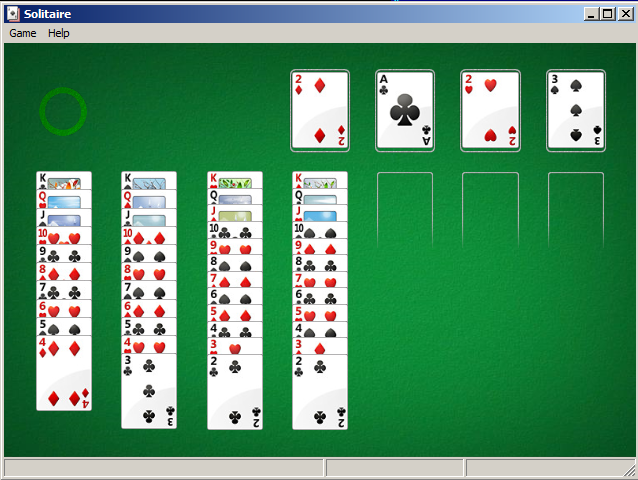
\includegraphics[width=0.6\textwidth]{examples/lines/1.png}
\caption{Обычный вид игры}
\label{fig:lines_1}
\end{figure}

\clearpage
\myindex{\CStandardLibrary!rand()}
Посмотрим, сможем ли мы найти генератор псевдослучайных чисел и и сделать с ним одну шутку.

\IDA быстро распознает стандартную функцию \TT{\_rand} в 
\TT{balltrix.exe} по адресу \TT{0x00403DA0}.
\IDA также показывает, что она вызывается только из одного места:

\lstinputlisting[style=customasmx86]{examples/lines/random.lst}

Назовем её \q{random}.
Пока не будем концентрироваться на самом коде функции.

Эта функция вызывается из трех мест.

Вот первые два:

\lstinputlisting[style=customasmx86]{examples/lines/1.lst}

Вот третье:

\lstinputlisting[style=customasmx86]{examples/lines/2.lst}

Так что у функции только один аргумент.
10 передается в первых двух случаях и 5 в третьем.

Мы также можем заметить, что размер доски 10*10 и здесь 5 возможных цветов.
Это оно!
Стандартная функция \TT{rand()} возвращает число в пределах \TT{0..0x7FFF} и это неудобно, так что многие программисты пишут свою функцию,
возвращающую случайное число в некоторых заданных пределах.
В нашем случае, предел это $0..n-1$ и $n$ передается как
единственный аргумент в функцию.
Мы можем быстро проверить это в отладчике.

Сделаем так, чтобы третий вызов функции всегда возвращал ноль.
В начале заменим три инструкции (\TT{PUSH/CALL/ADD}) 
на \ac{NOP}s.
Затем добавим инструкцию \INS{XOR EAX, EAX}, для очистки регистра \EAX.

\lstinputlisting[style=customasmx86]{examples/lines/fixed.lst}

Что мы сделали, это заменили вызов функции \TT{random()} 
на код, всегда возвращающий ноль.

\clearpage
Теперь запустим:

\begin{figure}[H]
\centering
\includegraphics[width=0.6\textwidth]{examples/lines/2.png}
\caption{Шутка сработала}
\end{figure}

О да, это работает\footnote{Автор этой книги однажды сделал это как 
шутку для его сотрудников, в надежде что они перестанут играть. 
Надежды не оправдались.}.

Но почему аргументы функции \TT{random()} это глобальные переменные?
Это просто потому что в настройках игры можно изменять размер доски, так что эти параметры не фиксированы.
10 и 5 это просто значения по умолчанию.

\mysection{\MinesweeperWinXPExampleChapterName}
\label{minesweeper_winxp}
\myindex{Windows!Windows XP}

Для тех, кто не очень хорошо играет в Сапёра (Minesweeper), можно попробовать найти все скрытые мины в отладчике.

\myindex{\CStandardLibrary!rand()}
\myindex{Windows!PDB}
Как мы знаем, Сапёр располагает мины случайным образом, так что там должен быть генератор случайных чисел
или вызов стандартной функции Си \TT{rand()}.

Вот что хорошо в реверсинге продуктов от Microsoft, так это то что часто есть \gls{PDB}-файл со всеми
символами (имена функций, и~т.д.).

Когда мы загружаем \TT{winmine.exe} в \IDA, она скачивает 
\gls{PDB} файл именно для этого исполняемого файла и добавляет все имена.

И вот оно, только один вызов \TT{rand()} в этой функции:

\lstinputlisting[style=customasmx86]{examples/minesweeper/tmp1.lst}

Так её назвала \IDA и это было имя данное ей разработчиками Сапёра.

Функция очень простая:

\begin{lstlisting}[style=customc]
int Rnd(int limit)
{
    return rand() % limit;
};
\end{lstlisting}

(В \gls{PDB}-файле не было имени \q{limit}; это мы назвали этот аргумент так, вручную.)

Так что она возвращает случайное число в пределах от нуля до заданного предела.

\TT{Rnd()} вызывается только из одного места, это функция с названием \TT{StartGame()}, 
и как видно, это именно тот код, что расставляет мины:

\begin{lstlisting}[style=customasmx86]
.text:010036C7                 push    _xBoxMac
.text:010036CD                 call    _Rnd@4          ; Rnd(x)
.text:010036D2                 push    _yBoxMac
.text:010036D8                 mov     esi, eax
.text:010036DA                 inc     esi
.text:010036DB                 call    _Rnd@4          ; Rnd(x)
.text:010036E0                 inc     eax
.text:010036E1                 mov     ecx, eax
.text:010036E3                 shl     ecx, 5          ; ECX=ECX*32
.text:010036E6                 test    _rgBlk[ecx+esi], 80h
.text:010036EE                 jnz     short loc_10036C7
.text:010036F0                 shl     eax, 5          ; EAX=EAX*32
.text:010036F3                 lea     eax, _rgBlk[eax+esi]
.text:010036FA                 or      byte ptr [eax], 80h
.text:010036FD                 dec     _cBombStart
.text:01003703                 jnz     short loc_10036C7
\end{lstlisting}

Сапёр позволяет задать размеры доски, так что X (xBoxMac) и Y (yBoxMac) это глобальные переменные.

Они передаются в \TT{Rnd()} и генерируются случайные координаты.
Мина устанавливается инструкцией \TT{OR} на \TT{0x010036FA}. 
И если она уже была установлена до этого 
(это возможно, если пара функций \TT{Rnd()} 
сгенерирует пару, которая уже была сгенерирована), 
тогда \TT{TEST} и \TT{JNZ} на \TT{0x010036E6} 
перейдет на повторную генерацию пары.

\TT{cBombStart} это глобальная переменная, содержащая количество мин. Так что это цикл.

Ширина двухмерного массива это 32 (мы можем это вывести, глядя на инструкцию \TT{SHL}, которая умножает
одну из координат на 32).

Размер глобального массива \TT{rgBlk} 
можно легко узнать по разнице между меткой \TT{rgBlk} 
в сегменте данных и следующей известной меткой. 
Это 0x360 (864):

\begin{lstlisting}[style=customasmx86]
.data:01005340 _rgBlk          db 360h dup(?)          ; DATA XREF: MainWndProc(x,x,x,x)+574
.data:01005340                                         ; DisplayBlk(x,x)+23
.data:010056A0 _Preferences    dd ?                    ; DATA XREF: FixMenus()+2
...
\end{lstlisting}

$864/32=27$.

Так что размер массива $27*32$?
Это близко к тому что мы знаем: если попытаемся установить размер доски в установках Сапёра на $100*100$, то он установит размер $24*30$.
Так что это максимальный размер доски здесь.
И размер массива фиксирован для доски любого размера.

Посмотрим на всё это в \olly.
Запустим Сапёр, присоединим (attach) \olly к нему и увидим содержимое памяти по адресу где массив \TT{rgBlk} (\TT{0x01005340})%

\footnote{Все адреса здесь для Сапёра под Windows XP SP3 English. 
Они могут отличаться для других сервис-паков.}.

Так что у нас выходит такой дамп памяти массива:

\lstinputlisting[style=customasmx86]{examples/minesweeper/1.lst}

\olly, как и любой другой шестнадцатеричный редактор, показывает 16 байт на строку.
Так что каждая 32-байтная строка массива занимает ровно 2 строки.

Это уровень для начинающих (доска 9*9).

Тут еще какая-то квадратная структура, заметная визуально (байты 0x10).

Нажмем \q{Run} в \olly чтобы разморозить процесс Сапёра, потом нажмем в случайное место окна Сапёра, попадаемся на мине, но теперь
видны все мины:

\begin{figure}[H]
\centering
\myincludegraphicsSmall{examples/minesweeper/1.png}
\caption{Мины}
\label{fig:minesweeper1}
\end{figure}

Сравнивая места с минами и дамп, мы можем обнаружить что 0x10 это граница, 0x0F --- пустой блок, 
0x8F --- мина.
Вероятно 0x10 это т.н., \emph{sentinel value}.

Теперь добавим комментариев и также заключим все байты 0x8F в квадратные скобки:%

\lstinputlisting[style=customasmx86]{examples/minesweeper/2.lst}

Теперь уберем все байты связанные с границами (0x10) и всё что за ними:%

\lstinputlisting[style=customasmx86]{examples/minesweeper/3.lst}

Да, это всё мины, теперь это очень хорошо видно, в сравнении со скриншотом.

\clearpage
Вот что интересно, это то что мы можем модифицировать массив прямо в \olly.%

Уберем все мины заменив все байты 0x8F на 0x0F, и вот что получится в Сапёре:

\begin{figure}[H]
\centering
\myincludegraphicsSmall{examples/minesweeper/3.png}
\caption{Все мины убраны в отладчике}
\label{fig:minesweeper3}
\end{figure}

Также уберем их все и добавим их в первом ряду: 

\begin{figure}[H]
\centering
\myincludegraphicsSmall{examples/minesweeper/2.png}
\caption{Мины, установленные в отладчике}
\label{fig:minesweeper2}
\end{figure}

Отладчик не очень удобен для подсматривания (а это была наша изначальная цель), так что напишем маленькую
утилиту для показа содержимого доски:

\lstinputlisting[style=customc]{examples/minesweeper/minesweeper_cheater.c}

Просто установите \ac{PID}
\footnote{PID можно увидеть в Task Manager 
(это можно включить в \q{View $\rightarrow$ Select Columns})} 
и адрес массива (\TT{0x01005340} для Windows XP SP3 English) 
и она покажет его
\footnote{Скомпилированная версия здесь: 
\href{http://beginners.re/examples/minesweeper_WinXP/minesweeper_cheater.exe}{beginners.re}}.

Она подключается к win32-процессу по \ac{PID}-у и просто читает из памяти процесса по этому адресу.

\subsection{Автоматический поиск массива}

Задавать адрес каждый раз при запуске нашей утилиты, это неудобно.
К тому же, разные версии ``Сапёра'' могут иметь этот массив по разным адресам.
Зная, что всегда есть рамка (байты 0x10), массив легко найти в памяти:

\lstinputlisting[style=customc]{examples/minesweeper/cheater2_fragment.c}

Полный исходный код: \url{\RepoURL/examples/minesweeper/minesweeper_cheater2.c}.

\subsection{\Exercises}

\begin{itemize}

\item
Почему байты описывающие границы (0x10) (или \emph{sentinel value}) присутствуют вообще?
Зачем они нужны, если они вообще не видимы в интерфейсе Сапёра?
Как можно обойтись без них?

\item
Как выясняется, здесь больше возможных значений (для открытых блоков, для тех на которых игрок установил
флажок, и~т.д.).
	
Попробуйте найти значение каждого.

\item Измените мою утилиту так, чтобы она в запущенном процессе Сапёра убирала все мины, 
или расставляла их в соответствии с каким-то заданным шаблоном.

\end{itemize}

\mysection{Хакаем часы в Windows}

Иногда я устраиваю первоапрельские пранки для моих сотрудников.

Посмотрим, можем ли мы сделать что-то с часами в Windows?
Можем ли мы их заставить идти в обратную сторону?

Прежде всего, когда вы кликаете на часы/время в строке состояния (\emph{status bar}),\\
запускается модуль \emph{C:\textbackslash{}WINDOWS\textbackslash{}SYSTEM32\textbackslash{}TIMEDATE.CPL},
а это обычный \ac{PE}-файл.

Посмотрим, как отрисовываются стрелки?
Когда я открываю этот файл (из Windows 7) в Resource Hacker, здесь есть разные виды циферблата, но нет стрелок:

\begin{figure}[H]
\centering
\myincludegraphics{examples/timedate/reshack.png}
\caption{Resource Hacker}
\end{figure}

ОК, что мы знаем? Как рисовать стрелку часов? Они все начинаются в середине круга и заканчиваются на его границе.
Следовательно, нам нужно расчитать координаты точки на границе круга.
Из школьной математики мы можем вспомнить, что для рисования круга нужно использовать ф-ции синуса/косинуса, или
хотя бы квадратного корня.
Такого в \emph{TIMEDATE.CPL} нет, по крайней мере на первый взгляд.
Но, благодаря отладочным PDB-файлам от Microsoft, я могу найти ф-цию с названием \emph{CAnalogClock::DrawHand()}, которая
вызывает \emph{Gdiplus::Graphics::DrawLine()} минимум дважды.

Вот её код:

\lstinputlisting[style=customasmx86]{examples/timedate/1.lst}

\myindex{Windows!Win32!MulDiv()}
Мы можем увидеть что аргументы \emph{DrawLine()} зависят от результата ф-ции \emph{MulDiv()}
и таблицы \emph{table[]} (название дал я),
которая содержит 8-байтные элементы (посмотрите на второй операнд \INS{LEA}).

Что внутри table[]?

\lstinputlisting[style=customasmx86]{examples/timedate/2.lst}

Доступ к ней есть только из ф-ции \emph{DrawHand()}.
У ней 120 32-битных слов или 60 32-битных пар \dots подождите, 60?
Посмотрим ближе на эти значения.
Прежде всего, я затру нулями первые 6 пар или 12 32-битных слов, и затем я положу пропатченный \emph{TIMEDATE.CPL}
в \emph{C:\textbackslash{}WINDOWS\textbackslash{}SYSTEM32}.
(Вам, возможно, придется установить владельца файла *TIMEDATE.CPL* равным вашей первичной пользовательской учетной
записи (вместо \emph{TrustedInstaller}),
а также загрузиться в безопасном режиме с командной строкой, чтобы скопировать этот файл, который обычно залоченный.)

\begin{figure}[H]
\centering
\includegraphics[width=0.5\textwidth]{examples/timedate/6_pairs_zeroed.png}
\caption{Attempt to run}
\end{figure}

Теперь, когда стрелка находится на 0..5 секундах/минутах, она невидимая! Хотя, противоположная (короткая) часть секундной
стрелки видима, и двигается.
Когда любая стрелка за пределами этой области, она видима, как обычно.

\myindex{Mathematica}
Посмотрим на эту таблицу при помощи Mathematica.
Я скопировал таблицу из \emph{TIMEDATE.CPL} в файл \emph{tbl} (480 байт).
Будем считать, что это знаковые значения, потому что половина элементов меньше нуля (0FFFFE0C1h, итд.).
Если бы эти значения были бы беззнаковыми, они были бы подозрительно большими.

\begin{lstlisting}[style=custommath]
In[]:= tbl = BinaryReadList["~/.../tbl", "Integer32"]

Out[]= {0, -7999, 836, -7956, 1663, -7825, 2472, -7608, 3253, -7308, 3999, \
-6928, 4702, -6472, 5353, -5945, 5945, -5353, 6472, -4702, 6928, \
-4000, 7308, -3253, 7608, -2472, 7825, -1663, 7956, -836, 8000, 0, \
7956, 836, 7825, 1663, 7608, 2472, 7308, 3253, 6928, 4000, 6472, \
4702, 5945, 5353, 5353, 5945, 4702, 6472, 3999, 6928, 3253, 7308, \
2472, 7608, 1663, 7825, 836, 7956, 0, 7999, -836, 7956, -1663, 7825, \
-2472, 7608, -3253, 7308, -4000, 6928, -4702, 6472, -5353, 5945, \
-5945, 5353, -6472, 4702, -6928, 3999, -7308, 3253, -7608, 2472, \
-7825, 1663, -7956, 836, -7999, 0, -7956, -836, -7825, -1663, -7608, \
-2472, -7308, -3253, -6928, -4000, -6472, -4702, -5945, -5353, -5353, \
-5945, -4702, -6472, -3999, -6928, -3253, -7308, -2472, -7608, -1663, \
-7825, -836, -7956}

In[]:= Length[tbl]
Out[]= 120
\end{lstlisting}

Будем считать два последовательно идущих 32-битных значения как пару:

\begin{lstlisting}[style=custommath]
In[]:= pairs = Partition[tbl, 2]
Out[]= {{0, -7999}, {836, -7956}, {1663, -7825}, {2472, -7608}, \
{3253, -7308}, {3999, -6928}, {4702, -6472}, {5353, -5945}, {5945, \
-5353}, {6472, -4702}, {6928, -4000}, {7308, -3253}, {7608, -2472}, \
{7825, -1663}, {7956, -836}, {8000, 0}, {7956, 836}, {7825, 
1663}, {7608, 2472}, {7308, 3253}, {6928, 4000}, {6472, 
4702}, {5945, 5353}, {5353, 5945}, {4702, 6472}, {3999, 
6928}, {3253, 7308}, {2472, 7608}, {1663, 7825}, {836, 7956}, {0, 
7999}, {-836, 7956}, {-1663, 7825}, {-2472, 7608}, {-3253, 
7308}, {-4000, 6928}, {-4702, 6472}, {-5353, 5945}, {-5945, 
5353}, {-6472, 4702}, {-6928, 3999}, {-7308, 3253}, {-7608, 
2472}, {-7825, 1663}, {-7956, 836}, {-7999, 
0}, {-7956, -836}, {-7825, -1663}, {-7608, -2472}, {-7308, -3253}, \
{-6928, -4000}, {-6472, -4702}, {-5945, -5353}, {-5353, -5945}, \
{-4702, -6472}, {-3999, -6928}, {-3253, -7308}, {-2472, -7608}, \
{-1663, -7825}, {-836, -7956}}

In[]:= Length[pairs]
Out[]= 60
\end{lstlisting}

Попробуем считать каждую пару как координату X/Y и нарисуем все 60 пар, а также первые 15 пар:

\begin{figure}[H]
\centering
\myincludegraphics{examples/timedate/math.png}
\caption{Mathematica}
\end{figure}

Ну теперь это кое-что!
Каждая пара это просто координата.
Первые 15 пар это координаты $\frac{1}{4}$ круга.

Видимо, разработчики в Microsoft расчитали все координаты предварительно и сохранили их в таблице.
\myindex{Memoization}
Это распространенная, хотя и немного олдскульная практика -- доступ к предвычисленным значениям в таблице быстрее, чем вызывать относительно медленные ф-ции
синуса/косинуса\footnote{Сегодня это называют \emph{memoization}}.
В наше время операции синуса/косинуса уже не такие \emph{дорогие}.

Теперь понятно, почему когда я затер первые 6 пар, стрелки были невидимы в этой области: на самом деле, стрелки рисовались,
просто их длина была нулевой, потому что стрелка начиналась в координатах 0:0, и там же и заканчивалась.

\subsubsection{Пранк (шутка)}

Учитывая всё это, можем ли мы заставить стрелки идти в обратную сторону?
На самом деле, это просто, нужно просто развернуть таблицу, так что каждая стрелка,
вместо отображения на месте нулевой секунды, рисовалась бы на месте 59-й секунды.

Когда-то давным давно я сделал патчер, в в самом начале 2000-х, для Windows 2000.
Трудно поверить, но он всё еще работает и для Windows 7, видимо, таблица с тех пор не менялась!

Исходник патчера: \url{\RepoURL/examples/timedate/time_pt.c}.

Теперь видно как стрелки идут назад:

\begin{figure}[H]
\centering
\includegraphics[width=0.5\textwidth]{examples/timedate/counterclockwise.png}
\caption{Now it works}
\end{figure}

В этой книге, конечно, нет анимации, но если присмотритесь, увидите, что на самом деле стрелки показывают корректное время,
но весь циферблат повернут вертикально, как если бы мы видели его изнутри часов.

\subsubsection{Утекшие исходники Windows 2000}

Так что я сделал патчер, потом утекли исходники Windows 2000 (я не могу заставить вас поверить мне, конечно).
Посмотрим на исходный код этой ф-ции и таблицы.\\
Нужный файл это \emph{win2k/private/shell/cpls/utc/clock.c}:

\begin{lstlisting}[style=customc]
//
//  Array containing the sine and cosine values for hand positions.
//
POINT rCircleTable[] =
{
    { 0,     -7999},
    { 836,   -7956},
    { 1663,  -7825},
    { 2472,  -7608},
    { 3253,  -7308},
...
    { -4702, -6472},
    { -3999, -6928},
    { -3253, -7308},
    { -2472, -7608},
    { -1663, -7825},
    { -836 , -7956},
};

////////////////////////////////////////////////////////////////////////////
//
//  DrawHand
//
//  Draws the hands of the clock.
//
////////////////////////////////////////////////////////////////////////////

void DrawHand(
    HDC hDC,
    int pos,
    HPEN hPen,
    int scale,
    int patMode,
    PCLOCKSTR np)
{
    LPPOINT lppt;
    int radius;

    MoveTo(hDC, np->clockCenter.x, np->clockCenter.y);
    radius = MulDiv(np->clockRadius, scale, 100);
    lppt = rCircleTable + pos;
    SetROP2(hDC, patMode);
    SelectObject(hDC, hPen);

    LineTo( hDC,
            np->clockCenter.x + MulDiv(lppt->x, radius, 8000),
            np->clockCenter.y + MulDiv(lppt->y, radius, 8000) );
}
\end{lstlisting}

Теперь всё ясно: координаты были предвычислены, как если бы циферблат был размером $2 \cdot 8000$,
а затем он масштабируется до радиуса текущего циферблата используя ф-цию \emph{MulDiv()}.

Структура POINT\footnote{\url{https://msdn.microsoft.com/en-us/library/windows/desktop/dd162805(v=vs.85).aspx}}
это структура из двух 32-битных значений, первое это \emph{x}, второе это \emph{y}.


%\subsubsection{std::string}
\myindex{\Cpp!STL!std::string}
\label{std_string}

\myparagraph{Как устроена структура}

Многие строковые библиотеки \InSqBrackets{\CNotes 2.2} обеспечивают структуру содержащую ссылку 
на буфер собственно со строкой, переменную всегда содержащую длину строки 
(что очень удобно для массы функций \InSqBrackets{\CNotes 2.2.1}) и переменную содержащую текущий размер буфера.

Строка в буфере обыкновенно оканчивается нулем: это для того чтобы указатель на буфер можно было
передавать в функции требующие на вход обычную сишную \ac{ASCIIZ}-строку.

Стандарт \Cpp не описывает, как именно нужно реализовывать std::string,
но, как правило, они реализованы как описано выше, с небольшими дополнениями.

Строки в \Cpp это не класс (как, например, QString в Qt), а темплейт (basic\_string), 
это сделано для того чтобы поддерживать 
строки содержащие разного типа символы: как минимум \Tchar и \emph{wchar\_t}.

Так что, std::string это класс с базовым типом \Tchar.

А std::wstring это класс с базовым типом \emph{wchar\_t}.

\mysubparagraph{MSVC}

В реализации MSVC, вместо ссылки на буфер может содержаться сам буфер (если строка короче 16-и символов).

Это означает, что каждая короткая строка будет занимать в памяти по крайней мере $16 + 4 + 4 = 24$ 
байт для 32-битной среды либо $16 + 8 + 8 = 32$ 
байта в 64-битной, а если строка длиннее 16-и символов, то прибавьте еще длину самой строки.

\lstinputlisting[caption=пример для MSVC,style=customc]{\CURPATH/STL/string/MSVC_RU.cpp}

Собственно, из этого исходника почти всё ясно.

Несколько замечаний:

Если строка короче 16-и символов, 
то отдельный буфер для строки в \glslink{heap}{куче} выделяться не будет.

Это удобно потому что на практике, основная часть строк действительно короткие.
Вероятно, разработчики в Microsoft выбрали размер в 16 символов как разумный баланс.

Теперь очень важный момент в конце функции main(): мы не пользуемся методом c\_str(), тем не менее,
если это скомпилировать и запустить, то обе строки появятся в консоли!

Работает это вот почему.

В первом случае строка короче 16-и символов и в начале объекта std::string (его можно рассматривать
просто как структуру) расположен буфер с этой строкой.
\printf трактует указатель как указатель на массив символов оканчивающийся нулем и поэтому всё работает.

Вывод второй строки (длиннее 16-и символов) даже еще опаснее: это вообще типичная программистская ошибка 
(или опечатка), забыть дописать c\_str().
Это работает потому что в это время в начале структуры расположен указатель на буфер.
Это может надолго остаться незамеченным: до тех пока там не появится строка 
короче 16-и символов, тогда процесс упадет.

\mysubparagraph{GCC}

В реализации GCC в структуре есть еще одна переменная --- reference count.

Интересно, что указатель на экземпляр класса std::string в GCC указывает не на начало самой структуры, 
а на указатель на буфера.
В libstdc++-v3\textbackslash{}include\textbackslash{}bits\textbackslash{}basic\_string.h 
мы можем прочитать что это сделано для удобства отладки:

\begin{lstlisting}
   *  The reason you want _M_data pointing to the character %array and
   *  not the _Rep is so that the debugger can see the string
   *  contents. (Probably we should add a non-inline member to get
   *  the _Rep for the debugger to use, so users can check the actual
   *  string length.)
\end{lstlisting}

\href{http://gcc.gnu.org/onlinedocs/libstdc++/libstdc++-html-USERS-4.4/a01068.html}{исходный код basic\_string.h}

В нашем примере мы учитываем это:

\lstinputlisting[caption=пример для GCC,style=customc]{\CURPATH/STL/string/GCC_RU.cpp}

Нужны еще небольшие хаки чтобы сымитировать типичную ошибку, которую мы уже видели выше, из-за
более ужесточенной проверки типов в GCC, тем не менее, printf() работает и здесь без c\_str().

\myparagraph{Чуть более сложный пример}

\lstinputlisting[style=customc]{\CURPATH/STL/string/3.cpp}

\lstinputlisting[caption=MSVC 2012,style=customasmx86]{\CURPATH/STL/string/3_MSVC_RU.asm}

Собственно, компилятор не конструирует строки статически: да в общем-то и как
это возможно, если буфер с ней нужно хранить в \glslink{heap}{куче}?

Вместо этого в сегменте данных хранятся обычные \ac{ASCIIZ}-строки, а позже, во время выполнения, 
при помощи метода \q{assign}, конструируются строки s1 и s2
.
При помощи \TT{operator+}, создается строка s3.

Обратите внимание на то что вызов метода c\_str() отсутствует,
потому что его код достаточно короткий и компилятор вставил его прямо здесь:
если строка короче 16-и байт, то в регистре EAX остается указатель на буфер,
а если длиннее, то из этого же места достается адрес на буфер расположенный в \glslink{heap}{куче}.

Далее следуют вызовы трех деструкторов, причем, они вызываются только если строка длиннее 16-и байт:
тогда нужно освободить буфера в \glslink{heap}{куче}.
В противном случае, так как все три объекта std::string хранятся в стеке,
они освобождаются автоматически после выхода из функции.

Следовательно, работа с короткими строками более быстрая из-за м\'{е}ньшего обращения к \glslink{heap}{куче}.

Код на GCC даже проще (из-за того, что в GCC, как мы уже видели, не реализована возможность хранить короткую
строку прямо в структуре):

% TODO1 comment each function meaning
\lstinputlisting[caption=GCC 4.8.1,style=customasmx86]{\CURPATH/STL/string/3_GCC_RU.s}

Можно заметить, что в деструкторы передается не указатель на объект,
а указатель на место за 12 байт (или 3 слова) перед ним, то есть, на настоящее начало структуры.

\myparagraph{std::string как глобальная переменная}
\label{sec:std_string_as_global_variable}

Опытные программисты на \Cpp знают, что глобальные переменные \ac{STL}-типов вполне можно объявлять.

Да, действительно:

\lstinputlisting[style=customc]{\CURPATH/STL/string/5.cpp}

Но как и где будет вызываться конструктор \TT{std::string}?

На самом деле, эта переменная будет инициализирована даже перед началом \main.

\lstinputlisting[caption=MSVC 2012: здесь конструируется глобальная переменная{,} а также регистрируется её деструктор,style=customasmx86]{\CURPATH/STL/string/5_MSVC_p2.asm}

\lstinputlisting[caption=MSVC 2012: здесь глобальная переменная используется в \main,style=customasmx86]{\CURPATH/STL/string/5_MSVC_p1.asm}

\lstinputlisting[caption=MSVC 2012: эта функция-деструктор вызывается перед выходом,style=customasmx86]{\CURPATH/STL/string/5_MSVC_p3.asm}

\myindex{\CStandardLibrary!atexit()}
В реальности, из \ac{CRT}, еще до вызова main(), вызывается специальная функция,
в которой перечислены все конструкторы подобных переменных.
Более того: при помощи atexit() регистрируется функция, которая будет вызвана в конце работы программы:
в этой функции компилятор собирает вызовы деструкторов всех подобных глобальных переменных.

GCC работает похожим образом:

\lstinputlisting[caption=GCC 4.8.1,style=customasmx86]{\CURPATH/STL/string/5_GCC.s}

Но он не выделяет отдельной функции в которой будут собраны деструкторы: 
каждый деструктор передается в atexit() по одному.

% TODO а если глобальная STL-переменная в другом модуле? надо проверить.


\mysection{\RU{Донглы}\EN{Dongles}}
\label{dongles}

% TODO dongle picture

\RU{Автор этих строк иногда делал замену \glslink{dongle}{донглам} или \q{эмуляторы донглов} 
и здесь немного примеров, как это происходит.}
\EN{The author of these lines, occasionally did software copy-protection \gls{dongle} replacements, or \q{dongle emulators} and here
are couple examples of how it's happening.}

\RU{Об одном неописанном здесь случае с Rockey и Z3 вы также можете прочитать здесь}
\EN{About one of the cases about Rocket and Z3 that is not present here, you can read here}:
\url{http://yurichev.com/tmp/SAT_SMT_DRAFT.pdf}.

\EN{\input{examples/dongles/1/main_EN}}
\RU{\input{examples/dongles/1/main_RU}}
\EN{\input{examples/dongles/2/main_EN}}

\RU{\input{examples/dongles/2/main_RU}}
\EN{\input{examples/dongles/3/main_EN}}
\RU{\input{examples/dongles/3/main_RU}}



% I never liked this part:
% \mysection{\q{QR9}: Любительская криптосистема, вдохновленная кубиком Рубика}

Любительские криптосистемы иногда встречаются довольно странные.

Однажды автора сих строк попросили разобраться с одним таким любительским криптоалгоритмом встроенным в 
утилиту для шифрования, исходный код которой был утерян\footnote{Он также получил разрешение от 
клиента на публикацию деталей алгоритма}.

Вот листинг этой утилиты для шифрования, полученный при помощи \IDA:

% TODO translate:
\lstinputlisting[style=customasmx86]{examples/qr9/qr9_original.lst}

Все имена функций и меток даны мною в процессе анализа.

Начнем с самого верха. Вот функция, берущая на вход два имени файла и пароль.


\begin{lstlisting}[style=customasmx86]
.text:00541320 ; int __cdecl crypt_file(char *Str, char *Filename, int password)
.text:00541320 crypt_file      proc near
.text:00541320
.text:00541320 Str             = dword ptr  4
.text:00541320 Filename        = dword ptr  8
.text:00541320 password        = dword ptr  0Ch
.text:00541320
\end{lstlisting}

Открыть файл и сообщить об ошибке в случае ошибки:

\begin{lstlisting}[style=customasmx86]
.text:00541320                 mov     eax, [esp+Str]
.text:00541324                 push    ebp
.text:00541325                 push    offset Mode     ; "rb"
.text:0054132A                 push    eax             ; Str
.text:0054132B                 call    _fopen          ; open file
.text:00541330                 mov     ebp, eax
.text:00541332                 add     esp, 8
.text:00541335                 test    ebp, ebp
.text:00541337                 jnz     short loc_541348
.text:00541339                 push    offset Format   ; "Cannot open input file!\n"
.text:0054133E                 call    _printf
.text:00541343                 add     esp, 4
.text:00541346                 pop     ebp
.text:00541347                 retn
.text:00541348
.text:00541348 loc_541348:
\end{lstlisting}

\myindex{\CStandardLibrary!fseek()}
\myindex{\CStandardLibrary!ftell()}
Узнать размер файла используя \TT{fseek()}/\TT{ftell()}:

\lstinputlisting[style=customasmx86]{examples/qr9/1_RU}

Этот фрагмент кода вычисляет длину файла, выровненную по 64-байтной границе.
Это потому что этот алгоритм шифрования работает только с блоками размерами 64 байта.
Работает очень просто: разделить длину файла на 64, забыть об остатке, прибавить 1,
умножить на 64.
Следующий код удаляет остаток от деления, как если бы это значение уже было разделено 
на 64 и добавляет 64. Это почти то же самое.

\lstinputlisting[style=customasmx86]{examples/qr9/2_RU}

Выделить буфер с выровненным размером:

\begin{lstlisting}[style=customasmx86]
.text:00541373                 push    esi             ; Size
.text:00541374                 call    _malloc
\end{lstlisting}

\myindex{\CStandardLibrary!calloc()}
Вызвать memset(), т.е. очистить выделенный буфер\footnote{malloc() + memset() можно было бы 
заменить на calloc()}.

\lstinputlisting[style=customasmx86]{examples/qr9/3_RU}

Чтение файла используя стандартную функцию Си \TT{fread()}.

\begin{lstlisting}[style=customasmx86]
.text:00541392                 mov     eax, [esp+38h+Str]
.text:00541396                 push    eax             ; ElementSize
.text:00541397                 push    ebx             ; DstBuf
.text:00541398                 call    _fread          ; read file
.text:0054139D                 push    ebp             ; File
.text:0054139E                 call    _fclose
\end{lstlisting}

Вызов \TT{crypt()}. Эта функция берет на вход буфер, длину буфера (выровненную) и строку пароля.

\begin{lstlisting}[style=customasmx86]
.text:005413A3                 mov     ecx, [esp+44h+password]
.text:005413A7                 push    ecx             ; password
.text:005413A8                 push    esi             ; aligned size
.text:005413A9                 push    ebx             ; buffer
.text:005413AA                 call    crypt           ; do crypt
\end{lstlisting}

Создать выходной файл. Кстати, разработчик забыл вставить проверку, создался ли файл успешно!
Результат открытия файла, впрочем, проверяется.

\begin{lstlisting}[style=customasmx86]
.text:005413AF                 mov     edx, [esp+50h+Filename]
.text:005413B3                 add     esp, 40h
.text:005413B6                 push    offset aWb      ; "wb"
.text:005413BB                 push    edx             ; Filename
.text:005413BC                 call    _fopen
.text:005413C1                 mov     edi, eax
\end{lstlisting}

Теперь хэндл созданного файла в регистре \EDI. Записываем сигнатуру \q{QR9}.

\begin{lstlisting}[style=customasmx86]
.text:005413C3                 push    edi             ; File
.text:005413C4                 push    1               ; Count
.text:005413C6                 push    3               ; Size
.text:005413C8                 push    offset aQr9     ; "QR9"
.text:005413CD                 call    _fwrite         ; write file signature
\end{lstlisting}

Записываем настоящую длину файла (не выровненную):

\begin{lstlisting}[style=customasmx86]
.text:005413D2                 push    edi             ; File
.text:005413D3                 push    1               ; Count
.text:005413D5                 lea     eax, [esp+30h+Str]
.text:005413D9                 push    4               ; Size
.text:005413DB                 push    eax             ; Str
.text:005413DC                 call    _fwrite         ; write original file size
\end{lstlisting}

Записываем шифрованный буфер:

\begin{lstlisting}[style=customasmx86]
.text:005413E1                 push    edi             ; File
.text:005413E2                 push    1               ; Count
.text:005413E4                 push    esi             ; Size
.text:005413E5                 push    ebx             ; Str
.text:005413E6                 call    _fwrite         ; write encrypted file
\end{lstlisting}

Закрыть файл и освободить выделенный буфер:

\begin{lstlisting}[style=customasmx86]
.text:005413EB                 push    edi             ; File
.text:005413EC                 call    _fclose
.text:005413F1                 push    ebx             ; Memory
.text:005413F2                 call    _free
.text:005413F7                 add     esp, 40h
.text:005413FA                 pop     edi
.text:005413FB                 pop     esi
.text:005413FC                 pop     ebx
.text:005413FD                 pop     ebp
.text:005413FE                 retn
.text:005413FE crypt_file      endp
\end{lstlisting}

Переписанный на Си код:

\begin{lstlisting}[style=customc]
void crypt_file(char *fin, char* fout, char *pw)
{
	FILE *f;
	int flen, flen_aligned;
	BYTE *buf;

	f=fopen(fin, "rb");
	
	if (f==NULL)
	{
		printf ("Cannot open input file!\n");
		return;
	};

	fseek (f, 0, SEEK_END);
	flen=ftell (f);
	fseek (f, 0, SEEK_SET);

	flen_aligned=(flen&0xFFFFFFC0)+0x40;

	buf=(BYTE*)malloc (flen_aligned);
	memset (buf, 0, flen_aligned);

	fread (buf, flen, 1, f);

	fclose (f);

	crypt (buf, flen_aligned, pw);
	
	f=fopen(fout, "wb");

	fwrite ("QR9", 3, 1, f);
	fwrite (&flen, 4, 1, f);
	fwrite (buf, flen_aligned, 1, f);

	fclose (f);

	free (buf);
};
\end{lstlisting}

Процедура дешифрования почти такая же:

\begin{lstlisting}[style=customasmx86]
.text:00541400 ; int __cdecl decrypt_file(char *Filename, int, void *Src)
.text:00541400 decrypt_file    proc near
.text:00541400
.text:00541400 Filename        = dword ptr  4
.text:00541400 arg_4           = dword ptr  8
.text:00541400 Src             = dword ptr  0Ch
.text:00541400
.text:00541400                 mov     eax, [esp+Filename]
.text:00541404                 push    ebx
.text:00541405                 push    ebp
.text:00541406                 push    esi
.text:00541407                 push    edi
.text:00541408                 push    offset aRb      ; "rb"
.text:0054140D                 push    eax             ; Filename
.text:0054140E                 call    _fopen
.text:00541413                 mov     esi, eax
.text:00541415                 add     esp, 8
.text:00541418                 test    esi, esi
.text:0054141A                 jnz     short loc_54142E
.text:0054141C                 push    offset aCannotOpenIn_0 ; "Cannot open input file!\n"
.text:00541421                 call    _printf
.text:00541426                 add     esp, 4
.text:00541429                 pop     edi
.text:0054142A                 pop     esi
.text:0054142B                 pop     ebp
.text:0054142C                 pop     ebx
.text:0054142D                 retn
.text:0054142E
.text:0054142E loc_54142E:
.text:0054142E                 push    2               ; Origin
.text:00541430                 push    0               ; Offset
.text:00541432                 push    esi             ; File
.text:00541433                 call    _fseek
.text:00541438                 push    esi             ; File
.text:00541439                 call    _ftell
.text:0054143E                 push    0               ; Origin
.text:00541440                 push    0               ; Offset
.text:00541442                 push    esi             ; File
.text:00541443                 mov     ebp, eax
.text:00541445                 call    _fseek
.text:0054144A                 push    ebp             ; Size
.text:0054144B                 call    _malloc
.text:00541450                 push    esi             ; File
.text:00541451                 mov     ebx, eax
.text:00541453                 push    1               ; Count
.text:00541455                 push    ebp             ; ElementSize
.text:00541456                 push    ebx             ; DstBuf
.text:00541457                 call    _fread
.text:0054145C                 push    esi             ; File
.text:0054145D                 call    _fclose
\end{lstlisting}

Проверяем сигнатуру (первые 3 байта):

\begin{lstlisting}[style=customasmx86]
.text:00541462                 add     esp, 34h
.text:00541465                 mov     ecx, 3
.text:0054146A                 mov     edi, offset aQr9_0 ; "QR9"
.text:0054146F                 mov     esi, ebx
.text:00541471                 xor     edx, edx
.text:00541473                 repe cmpsb
.text:00541475                 jz      short loc_541489
\end{lstlisting}

Сообщить об ошибке если сигнатура отсутствует:

\begin{lstlisting}[style=customasmx86]
.text:00541477                 push    offset aFileIsNotCrypt ; "File is not encrypted!\n"
.text:0054147C                 call    _printf
.text:00541481                 add     esp, 4
.text:00541484                 pop     edi
.text:00541485                 pop     esi
.text:00541486                 pop     ebp
.text:00541487                 pop     ebx
.text:00541488                 retn
.text:00541489
.text:00541489 loc_541489:
\end{lstlisting}

Вызвать \TT{decrypt()}.

\begin{lstlisting}[style=customasmx86]
.text:00541489                 mov     eax, [esp+10h+Src]
.text:0054148D                 mov     edi, [ebx+3]
.text:00541490                 add     ebp, 0FFFFFFF9h
.text:00541493                 lea     esi, [ebx+7]
.text:00541496                 push    eax             ; Src
.text:00541497                 push    ebp             ; int
.text:00541498                 push    esi             ; int
.text:00541499                 call    decrypt
.text:0054149E                 mov     ecx, [esp+1Ch+arg_4]
.text:005414A2                 push    offset aWb_0    ; "wb"
.text:005414A7                 push    ecx             ; Filename
.text:005414A8                 call    _fopen
.text:005414AD                 mov     ebp, eax
.text:005414AF                 push    ebp             ; File
.text:005414B0                 push    1               ; Count
.text:005414B2                 push    edi             ; Size
.text:005414B3                 push    esi             ; Str
.text:005414B4                 call    _fwrite
.text:005414B9                 push    ebp             ; File
.text:005414BA                 call    _fclose
.text:005414BF                 push    ebx             ; Memory
.text:005414C0                 call    _free
.text:005414C5                 add     esp, 2Ch
.text:005414C8                 pop     edi
.text:005414C9                 pop     esi
.text:005414CA                 pop     ebp
.text:005414CB                 pop     ebx
.text:005414CC                 retn
.text:005414CC decrypt_file    endp
\end{lstlisting}

Переписанный на Си код:

\begin{lstlisting}[style=customc]
void decrypt_file(char *fin, char* fout, char *pw)
{
	FILE *f;
	int real_flen, flen;
	BYTE *buf;

	f=fopen(fin, "rb");
	
	if (f==NULL)
	{
		printf ("Cannot open input file!\n");
		return;
	};

	fseek (f, 0, SEEK_END);
	flen=ftell (f);
	fseek (f, 0, SEEK_SET);

	buf=(BYTE*)malloc (flen);

	fread (buf, flen, 1, f);

	fclose (f);

	if (memcmp (buf, "QR9", 3)!=0)
	{
		printf ("File is not encrypted!\n");
		return;
	};

	memcpy (&real_flen, buf+3, 4);

	decrypt (buf+(3+4), flen-(3+4), pw);
	
	f=fopen(fout, "wb");

	fwrite (buf+(3+4), real_flen, 1, f);

	fclose (f);

	free (buf);
};
\end{lstlisting}

OK, посмотрим глубже.

Функция \TT{crypt()}:

\begin{lstlisting}[style=customasmx86]
.text:00541260 crypt           proc near
.text:00541260
.text:00541260 arg_0           = dword ptr  4
.text:00541260 arg_4           = dword ptr  8
.text:00541260 arg_8           = dword ptr  0Ch
.text:00541260
.text:00541260                 push    ebx
.text:00541261                 mov     ebx, [esp+4+arg_0]
.text:00541265                 push    ebp
.text:00541266                 push    esi
.text:00541267                 push    edi
.text:00541268                 xor     ebp, ebp
.text:0054126A
.text:0054126A loc_54126A:
\end{lstlisting}

\myindex{x86!\Instructions!MOVSD}
Этот фрагмент кода копирует часть входного буфера во внутренний буфер, который мы позже назовем \q{cube64}.%

Длина в регистре \ECX. \TT{MOVSD} означает \emph{скопировать 32-битное слово}, так что, 16 32-битных слов
это как раз 64 байта.

\begin{lstlisting}[style=customasmx86]
.text:0054126A                 mov     eax, [esp+10h+arg_8]
.text:0054126E                 mov     ecx, 10h
.text:00541273                 mov     esi, ebx   ; EBX is pointer within input buffer
.text:00541275                 mov     edi, offset cube64
.text:0054127A                 push    1
.text:0054127C                 push    eax
.text:0054127D                 rep movsd
\end{lstlisting}

Вызвать \TT{rotate\_all\_with\_password()}:

\begin{lstlisting}[style=customasmx86]
.text:0054127F                 call    rotate_all_with_password
\end{lstlisting}

Скопировать зашифрованное содержимое из \q{cube64} назад в буфер:

\begin{lstlisting}[style=customasmx86]
.text:00541284                 mov     eax, [esp+18h+arg_4]
.text:00541288                 mov     edi, ebx
.text:0054128A                 add     ebp, 40h
.text:0054128D                 add     esp, 8
.text:00541290                 mov     ecx, 10h
.text:00541295                 mov     esi, offset cube64
.text:0054129A                 add     ebx, 40h  ; add 64 to input buffer pointer
.text:0054129D                 cmp     ebp, eax  ; EBP = amount of encrypted data.
.text:0054129F                 rep movsd
\end{lstlisting}

Если \EBP не больше чем длина во входном аргументе, тогда переходим к следующему блоку.

\begin{lstlisting}[style=customasmx86]
.text:005412A1                 jl      short loc_54126A
.text:005412A3                 pop     edi
.text:005412A4                 pop     esi
.text:005412A5                 pop     ebp
.text:005412A6                 pop     ebx
.text:005412A7                 retn
.text:005412A7 crypt           endp
\end{lstlisting}

Реконструированная функция \TT{crypt()}:

\begin{lstlisting}[style=customc]
void crypt (BYTE *buf, int sz, char *pw)
{
	int i=0;
	
	do
	{
		memcpy (cube, buf+i, 8*8);
		rotate_all (pw, 1);
		memcpy (buf+i, cube, 8*8);
		i+=64;
	}
	while (i<sz);
};
\end{lstlisting}

OK, углубимся в функцию \TT{rotate\_all\_with\_password()}. Она берет на вход два аргумента: 
строку пароля и число.
В функции \TT{crypt()}, число 1 используется и в \TT{decrypt()} \\
(где \TT{rotate\_all\_with\_password()} функция вызывается также), число 3.

\begin{lstlisting}[style=customasmx86]
.text:005411B0 rotate_all_with_password proc near
.text:005411B0
.text:005411B0 arg_0           = dword ptr  4
.text:005411B0 arg_4           = dword ptr  8
.text:005411B0
.text:005411B0                 mov     eax, [esp+arg_0]
.text:005411B4                 push    ebp
.text:005411B5                 mov     ebp, eax
\end{lstlisting}

Проверяем символы в пароле. Если это ноль, выходим:

\begin{lstlisting}[style=customasmx86]
.text:005411B7                 cmp     byte ptr [eax], 0
.text:005411BA                 jz      exit
.text:005411C0                 push    ebx
.text:005411C1                 mov     ebx, [esp+8+arg_4]
.text:005411C5                 push    esi
.text:005411C6                 push    edi
.text:005411C7
.text:005411C7 loop_begin:
\end{lstlisting}

\myindex{\CStandardLibrary!tolower()}
Вызываем \TT{tolower()}, стандартную функцию Си.

\begin{lstlisting}[style=customasmx86]
.text:005411C7                 movsx   eax, byte ptr [ebp+0]
.text:005411CB                 push    eax             ; C
.text:005411CC                 call    _tolower
.text:005411D1                 add     esp, 4
\end{lstlisting}

Хмм, если пароль содержит символ не из латинского алфавита, он пропускается!
Действительно, если мы запускаем утилиту для шифрования используя символы не латинского алфавита, 
похоже, они просто игнорируются.

\begin{lstlisting}[style=customasmx86]
.text:005411D4                 cmp     al, 'a'
.text:005411D6                 jl      short next_character_in_password
.text:005411D8                 cmp     al, 'z'
.text:005411DA                 jg      short next_character_in_password
.text:005411DC                 movsx   ecx, al
\end{lstlisting}

Отнимем значение \q{a} (97) от символа.

\begin{lstlisting}[style=customasmx86]
.text:005411DF                 sub     ecx, 'a'  ; 97
\end{lstlisting}

После вычитания, тут будет 0 для \q{a}, 1 для \q{b}, и так далее. И 25 для \q{z}.

\begin{lstlisting}[style=customasmx86]
.text:005411E2                 cmp     ecx, 24
.text:005411E5                 jle     short skip_subtracting
.text:005411E7                 sub     ecx, 24
\end{lstlisting}

Похоже, символы \q{y} и \q{z} также исключительные.
После этого фрагмента кода, \q{y} становится 0, а \q{z} ~--- 1.
Это значит, что 26 латинских букв становятся значениями в интервале 0..23, (всего 24).

\begin{lstlisting}[style=customasmx86]
.text:005411EA
.text:005411EA skip_subtracting:                       ; CODE XREF: rotate_all_with_password+35
\end{lstlisting}

Это, на самом деле, деление через умножение.
Читайте об этом больше в секции \q{\DivisionByMultSectionName}~(\myref{sec:divisionbymult}).

Это код, на самом деле, делит значение символа пароля на 3.

% TODO1: add Mathematica calculations
\begin{lstlisting}[style=customasmx86]
.text:005411EA                 mov     eax, 55555556h
.text:005411EF                 imul    ecx
.text:005411F1                 mov     eax, edx
.text:005411F3                 shr     eax, 1Fh
.text:005411F6                 add     edx, eax
.text:005411F8                 mov     eax, ecx
.text:005411FA                 mov     esi, edx
.text:005411FC                 mov     ecx, 3
.text:00541201                 cdq
.text:00541202                 idiv    ecx
\end{lstlisting}

\EDX --- остаток от деления.

\lstinputlisting[style=customasmx86]{examples/qr9/4_RU}

Если остаток 2, вызываем \TT{rotate3()}. 
\EDX это второй аргумент функции \TT{rotate\_all\_with\_password()}. 
Как мы уже заметили, 1 это для шифрования, 3 для дешифрования.
Так что здесь цикл, функции rotate1/2/3 будут вызываться столько же раз, сколько значение переменной
в первом аргументе.

\begin{lstlisting}[style=customasmx86]
.text:00541215 call_rotate3:
.text:00541215                 push    esi
.text:00541216                 call    rotate3
.text:0054121B                 add     esp, 4
.text:0054121E                 dec     edi
.text:0054121F                 jnz     short call_rotate3
.text:00541221                 jmp     short next_character_in_password
.text:00541223
.text:00541223 call_rotate2:
.text:00541223                 test    ebx, ebx
.text:00541225                 jle     short next_character_in_password
.text:00541227                 mov     edi, ebx
.text:00541229
.text:00541229 loc_541229:
.text:00541229                 push    esi
.text:0054122A                 call    rotate2
.text:0054122F                 add     esp, 4
.text:00541232                 dec     edi
.text:00541233                 jnz     short loc_541229
.text:00541235                 jmp     short next_character_in_password
.text:00541237
.text:00541237 call_rotate1:
.text:00541237                 test    ebx, ebx
.text:00541239                 jle     short next_character_in_password
.text:0054123B                 mov     edi, ebx
.text:0054123D
.text:0054123D loc_54123D:
.text:0054123D                 push    esi
.text:0054123E                 call    rotate1
.text:00541243                 add     esp, 4
.text:00541246                 dec     edi
.text:00541247                 jnz     short loc_54123D
.text:00541249
\end{lstlisting}

Достать следующий символ из строки пароля.

\begin{lstlisting}[style=customasmx86]
.text:00541249 next_character_in_password:
.text:00541249                 mov     al, [ebp+1]
\end{lstlisting}

\glslink{increment}{Инкремент} указателя на символ в строке пароля:

\begin{lstlisting}[style=customasmx86]
.text:0054124C                 inc     ebp
.text:0054124D                 test    al, al
.text:0054124F                 jnz     loop_begin
.text:00541255                 pop     edi
.text:00541256                 pop     esi
.text:00541257                 pop     ebx
.text:00541258
.text:00541258 exit:
.text:00541258                 pop     ebp
.text:00541259                 retn
.text:00541259 rotate_all_with_password endp
\end{lstlisting}

Реконструированный код на Си:

\begin{lstlisting}[style=customc]
void rotate_all (char *pwd, int v)
{
	char *p=pwd;

	while (*p)
	{
		char c=*p;
		int q;

		c=tolower (c);

		if (c>='a' && c<='z')
		{
			q=c-'a';
			if (q>24)
				q-=24;

			int quotient=q/3;
			int remainder=q % 3;

			switch (remainder)
			{
			case 0: for (int i=0; i<v; i++) rotate1 (quotient); break;
			case 1: for (int i=0; i<v; i++) rotate2 (quotient); break;
			case 2: for (int i=0; i<v; i++) rotate3 (quotient); break;
			};
		};

		p++;
	};
};
\end{lstlisting}

Углубимся еще дальше и исследуем функции rotate1/2/3.
Каждая функция вызывает еще две.
В итоге мы назовем их \TT{set\_bit()} и \TT{get\_bit()}.

Начнем с \TT{get\_bit()}:

\begin{lstlisting}[style=customasmx86]
.text:00541050 get_bit         proc near
.text:00541050
.text:00541050 arg_0           = dword ptr  4
.text:00541050 arg_4           = dword ptr  8
.text:00541050 arg_8           = byte ptr  0Ch
.text:00541050
.text:00541050                 mov     eax, [esp+arg_4]
.text:00541054                 mov     ecx, [esp+arg_0]
.text:00541058                 mov     al, cube64[eax+ecx*8]
.text:0054105F                 mov     cl, [esp+arg_8]
.text:00541063                 shr     al, cl
.text:00541065                 and     al, 1
.text:00541067                 retn
.text:00541067 get_bit         endp
\end{lstlisting}

\dots иными словами: подсчитать индекс в массиве cube64: \emph{arg\_4 + arg\_0 * 8}.
Затем сдвинуть байт из массива вправо на количество бит заданных в arg\_8. 
Изолировать самый младший бит и вернуть его

Посмотрим другую функцию, \TT{set\_bit()}:

\begin{lstlisting}[style=customasmx86]
.text:00541000 set_bit         proc near
.text:00541000
.text:00541000 arg_0           = dword ptr  4
.text:00541000 arg_4           = dword ptr  8
.text:00541000 arg_8           = dword ptr  0Ch
.text:00541000 arg_C           = byte ptr  10h
.text:00541000
.text:00541000                 mov     al, [esp+arg_C]
.text:00541004                 mov     ecx, [esp+arg_8]
.text:00541008                 push    esi
.text:00541009                 mov     esi, [esp+4+arg_0]
.text:0054100D                 test    al, al
.text:0054100F                 mov     eax, [esp+4+arg_4]
.text:00541013                 mov     dl, 1
.text:00541015                 jz      short loc_54102B
\end{lstlisting}

\TT{DL} тут равно 1. Сдвигаем эту единицу на количество, указанное в arg\_8. Например, если в arg\_8 число 4,
тогда значение в \TT{DL} станет 0x10 или 1000b в двоичной системе счисления.

\begin{lstlisting}[style=customasmx86]
.text:00541017                 shl     dl, cl
.text:00541019                 mov     cl, cube64[eax+esi*8]
\end{lstlisting}

Вытащить бит из массива и явно выставить его. % TODO1: rewrite

\begin{lstlisting}[style=customasmx86]
.text:00541020                 or      cl, dl
\end{lstlisting}

Сохранить его назад: % TODO1: rewrite

\begin{lstlisting}[style=customasmx86]
.text:00541022                 mov     cube64[eax+esi*8], cl
.text:00541029                 pop     esi
.text:0054102A                 retn
.text:0054102B
.text:0054102B loc_54102B:
.text:0054102B                 shl     dl, cl
\end{lstlisting}

Если arg\_C не ноль\dots

\begin{lstlisting}[style=customasmx86]
.text:0054102D                 mov     cl, cube64[eax+esi*8]
\end{lstlisting}

\myindex{x86!\Instructions!NOT}
\dots инвертировать DL. Например, если состояние DL после сдвига 0x10 или 1000b в двоичной системе,
здесь будет 0xEF после инструкции \NOT или 11101111b в двоичной системе.

\begin{lstlisting}[style=customasmx86]
.text:00541034                 not     dl
\end{lstlisting}

Эта инструкция сбрасывает бит, иными словами, она сохраняет все биты в \TT{CL} которые также
выставлены в \TT{DL} кроме тех в \TT{DL}, что были сброшены. Это значит, что если в \TT{DL}, например,
11101111b в двоичной системе, все биты будут сохранены кроме пятого (считая с младшего бита).

\begin{lstlisting}[style=customasmx86]
.text:00541036                 and     cl, dl
\end{lstlisting}

Сохранить его назад

\begin{lstlisting}[style=customasmx86]
.text:00541038                 mov     cube64[eax+esi*8], cl
.text:0054103F                 pop     esi
.text:00541040                 retn
.text:00541040 set_bit         endp
\end{lstlisting}

Это почти то же самое что и \TT{get\_bit()}, кроме того, что если arg\_C ноль, тогда функция сбрасывает
указанный бит в массиве, либо же, в противном случае, выставляет его в 1.

Мы также знаем что размер массива 64. Первые два аргумента и у \TT{set\_bit()} и у \TT{get\_bit()}
могут быть представлены как двумерные координаты. Таким образом, массив ~--- это матрица 8*8.

Представление на Си всего того, что мы уже знаем:

\begin{lstlisting}[style=customc]
#define IS_SET(flag, bit)       ((flag) & (bit))
#define SET_BIT(var, bit)       ((var) |= (bit))
#define REMOVE_BIT(var, bit)    ((var) &= ~(bit))

static BYTE cube[8][8];

void set_bit (int x, int y, int shift, int bit)
{
	if (bit)
		SET_BIT (cube[x][y], 1<<shift);
	else
		REMOVE_BIT (cube[x][y], 1<<shift);
};

bool get_bit (int x, int y, int shift)
{
	if ((cube[x][y]>>shift)&1==1)
		return 1;
	return 0;
};
\end{lstlisting}

Теперь вернемся к функциям rotate1/2/3.

\begin{lstlisting}[style=customasmx86]
.text:00541070 rotate1         proc near
.text:00541070
\end{lstlisting}

Выделение внутреннего массива размером 64 байта в локальном стеке:

\begin{lstlisting}[style=customasmx86]
.text:00541070 internal_array_64= byte ptr -40h
.text:00541070 arg_0           = dword ptr  4
.text:00541070
.text:00541070                 sub     esp, 40h
.text:00541073                 push    ebx
.text:00541074                 push    ebp
.text:00541075                 mov     ebp, [esp+48h+arg_0]
.text:00541079                 push    esi
.text:0054107A                 push    edi
.text:0054107B                 xor     edi, edi        ; EDI is loop1 counter
\end{lstlisting}

\EBX указывает на внутренний массив

\begin{lstlisting}[style=customasmx86]
.text:0054107D                 lea     ebx, [esp+50h+internal_array_64]
.text:00541081
\end{lstlisting}

Здесь два вложенных цикла:

\lstinputlisting[style=customasmx86]{examples/qr9/5_RU}

Мы видим, что оба счетчика циклов в интервале 0..7. 
Также, они используются как первый и второй аргумент \TT{get\_bit()}.
Третий аргумент \TT{get\_bit()} это единственный аргумент \TT{rotate1()}. 
То что возвращает \TT{get\_bit()} будет сохранено во внутреннем массиве.

Снова приготовить указатель на внутренний массив:

\lstinputlisting[style=customasmx86]{examples/qr9/6_RU}

\dots этот код помещает содержимое из внутреннего массива в глобальный массив cube используя функцию 
\TT{set\_bit()}, \emph{но}, в обратном порядке!
Теперь счетчик первого цикла в интервале 7 до 0, уменьшается на 1 на каждой итерации!

Представление кода на Си выглядит так:

\begin{lstlisting}[style=customc]
void rotate1 (int v)
{
	bool tmp[8][8]; // internal array
	int i, j;

	for (i=0; i<8; i++)
		for (j=0; j<8; j++)
			tmp[i][j]=get_bit (i, j, v);

	for (i=0; i<8; i++)
		for (j=0; j<8; j++)
			set_bit (j, 7-i, v, tmp[x][y]);
};
\end{lstlisting}

Не очень понятно, но если мы посмотрим в функцию \TT{rotate2()}:

\lstinputlisting[style=customasmx86]{examples/qr9/7_RU}

\emph{Почти} то же самое, за исключением иного порядка аргументов в \TT{get\_bit()} и \TT{set\_bit()}.
Перепишем это на Си-подобный код:

\begin{lstlisting}[style=customc]
void rotate2 (int v)
{
	bool tmp[8][8]; // internal array
	int i, j;

	for (i=0; i<8; i++)
		for (j=0; j<8; j++)
			tmp[i][j]=get_bit (v, i, j);

	for (i=0; i<8; i++)
		for (j=0; j<8; j++)
			set_bit (v, j, 7-i, tmp[i][j]);
};
\end{lstlisting}

Перепишем так же функцию \TT{rotate3()}:

\begin{lstlisting}[style=customasmx86]
void rotate3 (int v)
{
	bool tmp[8][8];
	int i, j;

	for (i=0; i<8; i++)
		for (j=0; j<8; j++)
			tmp[i][j]=get_bit (i, v, j);

	for (i=0; i<8; i++)
		for (j=0; j<8; j++)
			set_bit (7-j, v, i, tmp[i][j]);
};
\end{lstlisting}

Теперь всё проще. Если мы представим cube64 как трехмерный куб 8*8*8, где каждый элемент это бит,
то \TT{get\_bit()} и \TT{set\_bit()} просто берут на вход координаты бита.

Функции rotate1/2/3 просто поворачивают все биты на определенной плоскости.
Три функции, каждая на каждую сторону куба и аргумент \TT{v} выставляет плоскость в интервале 0..7

Может быть, автор алгоритма думал о кубике Рубика 8*8*8

\footnote{\href{http://en.wikipedia.org/wiki/Rubik's_Cube}{wikipedia}}?!

Да, действительно.

Рассмотрим функцию \TT{decrypt()}, вот её переписанная версия:%

\begin{lstlisting}[style=customc]
void decrypt (BYTE *buf, int sz, char *pw)
{
	char *p=strdup (pw);
	strrev (p);
	int i=0;

	do
	{
		memcpy (cube, buf+i, 8*8);
		rotate_all (p, 3);
		memcpy (buf+i, cube, 8*8);
		i+=64;
	}
	while (i<sz);
	
	free (p);
};
\end{lstlisting}

Почти то же самое что и crypt(), \emph{но} строка пароля разворачивается стандартной функцией Си
strrev() \footnote{\href{http://msdn.microsoft.com/en-us/library/9hby7w40(VS.80).aspx}{MSDN}}
и \TT{rotate\_all()} вызывается с аргументом 3.

Это значит, что, в случае дешифровки, rotate1/2/3 будут вызываться трижды.

Это почти кубик Рубика!
Если вы хотите вернуть его состояние назад, делайте то же самое в обратном порядке и направлении!
Чтобы вернуть эффект от поворота плоскости по часовой стрелке, нужно повернуть её же против 
часовой стрелки, либо же трижды по часовой стрелке.

\TT{rotate1()}, вероятно, поворот \q{лицевой} плоскости. 
\TT{rotate2()}, вероятно, поворот \q{верхней} плоскости.
\TT{rotate3()}, вероятно, поворот \q{левой} плоскости.

Вернемся к ядру функции \TT{rotate\_all()}

\begin{lstlisting}[style=customc]
q=c-'a';
if (q>24)
	q-=24;

int quotient=q/3; // in range 0..7
int remainder=q % 3;

switch (remainder)
{
    case 0: for (int i=0; i<v; i++) rotate1 (quotient); break; // front
    case 1: for (int i=0; i<v; i++) rotate2 (quotient); break; // top
    case 2: for (int i=0; i<v; i++) rotate3 (quotient); break; // left
};
\end{lstlisting}

Так понять проще: каждый символ пароля определяет сторону (одну из трех) и плоскость (одну из восьми).
3*8 = 24, вот почему два последних символа латинского алфавита переопределяются так чтобы алфавит состоял
из 24-х элементов.

Алгоритм очевидно слаб: в случае коротких паролей, в бинарном редакторе файлов можно будет увидеть, 
что в зашифрованных файлах остались незашифрованные символы.

Весь исходный код в реконструированном виде:

\lstinputlisting[style=customc]{examples/qr9/qr9.cpp}



% TODO: OpenSSL tool, URLs, etc
\mysection{Случай с зашифрованной БД \#1}
\label{encrypted_DB1}

(Эта часть впервые появилась в моем блоге 26-Aug-2015.
Обсуждение: \url{https://news.ycombinator.com/item?id=10128684}.)

\subsection{Base64 и энтропия}

\myindex{XML}
Мне достался \ac{XML}-файл, содержащий некоторые зашифрованные данные.
Вероятно, что-то связанное с заказми и/или с информацией о клиентах.

\begin{lstlisting}
<?xml version = "1.0" encoding = "UTF-8"?>
<Orders>
	<Order>
		<OrderID>1</OrderID>
		<Data>yjmxhXUbhB/5MV45chPsXZWAJwIh1S0aD9lFn3XuJMSxJ3/E+UE3hsnH</Data>
	</Order>
	<Order>
		<OrderID>2</OrderID>
		<Data>0KGe/wnypFBjsy+U0C2P9fC5nDZP3XDZLMPCRaiBw9OjIk6Tu5U=</Data>
	</Order>
	<Order>
		<OrderID>3</OrderID>
		<Data>mqkXfdzvQKvEArdzh+zD9oETVGBFvcTBLs2ph1b5bYddExzp</Data>
	</Order>
	<Order>
		<OrderID>4</OrderID>
		<Data>FCx6JhIDqnESyT3HAepyE1BJ3cJd7wCk+APCRUeuNtZdpCvQ2MR/7kLXtfUHuA==</Data>
	</Order>
...
\end{lstlisting}

Файл доступен \href{https://raw.githubusercontent.com/DennisYurichev/RE-for-beginners/master/examples/encrypted_DB1/encrypted.xml}{здесь}.

\myindex{base64}
Это явно данные закодированные в base64, потому что все строки состоят из латинских символов, цифр,
и символов плюс (+) и слэш (/).
Могут быть еще два выравнивающих символа (=), но они никогда не встречаются в середине строки.
Зная эти свойства base64, такие строки легко распозновать.

Попробуем декодировать эти блоки и вычислить их энтропии (\myref{entropy}) при помощи Wolfram Mathematica:

\begin{lstlisting}
In[]:= ListOfBase64Strings =
  Map[First[#[[3]]] &, Cases[Import["encrypted.xml"], XMLElement["Data", _, _], Infinity]];

In[]:= BinaryStrings =
  Map[ImportString[#, {"Base64", "String"}] &, ListOfBase64Strings];

In[]:= Entropies = Map[N[Entropy[2, #]] &, BinaryStrings];

In[]:= Variance[Entropies]
Out[]= 0.0238614
\end{lstlisting}

\myindex{Variance}
Разброс (variance) низкий.
Это означает, что значения энтропии не очень отличаются друг от друга.
Это видно на графике:

\begin{lstlisting}
In[]:= ListPlot[Entropies]
\end{lstlisting}

\begin{figure}[H]
\centering
\myincludegraphics{examples/encrypted_DB1/entropy.png}
\end{figure}

Большинство значений между 5.0 и 5.4.
Это свидетельство того что данные сжаты и/или зашифрованы.

Чтобы понять разброс (variance), подсчитаем энтропии всех строк в книге Конана Дойля \emph{The Hound of the Baskervilles}:

\begin{lstlisting}
In[]:= BaskervillesLines = Import["http://www.gutenberg.org/cache/epub/2852/pg2852.txt", "List"];

In[]:= EntropiesT = Map[N[Entropy[2, #]] &, BaskervillesLines];

In[]:= Variance[EntropiesT]
Out[]= 2.73883

In[]:= ListPlot[EntropiesT]
\end{lstlisting}

\begin{figure}[H]
\centering
\myincludegraphics{examples/encrypted_DB1/conan_doyle.png}
\end{figure}

Большинство значений находится вокруг 4, но есть также м\'{е}ньшие значения, и они повлияли на конечное значение разброса.

Вероятно, самые короткие строки имеют м\'{е}ньшую энтропию, попробуем короткую строку из книги Конан Дойля:

\begin{lstlisting}
In[]:= Entropy[2, "Yes, sir."] // N
Out[]= 2.9477
\end{lstlisting}

Попробуем еще м\'{е}ньшую:

\begin{lstlisting}
In[]:= Entropy[2, "Yes"] // N
Out[]= 1.58496

In[]:= Entropy[2, "No"] // N
Out[]= 1.
\end{lstlisting}

\subsection{Данные сжаты?}

ОК, наши данные сжаты и/или зашифрованы.
Сжаты ли? Почти все компрессоры данных помещают некоторый заголовок в начале, сигнатуру или что-то вроде этого.
Как видим, здесь ничего такого нет в начале каждого блока.
Все еще возможно что это какой-то самодельный компрессор, но они очень редки.
С другой стороны, самодельные криптоалгоритмы попадаются часто, потому что их куда легче заставить работать.
\myindex{memfrob()}
\myindex{ROT13}
Даже примитивные криптосистемы без ключей, как \emph{memfrob()}\footnote{\url{http://linux.die.net/man/3/memfrob}}
и ROT13 нормально работают без ошибок.
А чтобы написать свой компрессор с нуля, используя только фантазию и воображение, так что он будет работать без ошибок,
это серьезная задача.
Некоторые программисты реализуют ф-ции сжатия данных по учебникам, но это также редкость.
Наиболее популярные способы это:
\myindex{zlib}
1) просто взять опен-сорсную библиотеку вроде zlib;
2) скопипастить что-то откуда-то.
Опен-сорсные алгоритмы сжатия данных обычно добавляют какой-то заголовок, и точно так же делают алгоритмы с сайтов вроде
\url{http://www.codeproject.com/}.

\subsection{Данные зашифрованы?}

Основные алгоритмы шифрования обрабатывают данные блоками. DES --- по 8 байт, AES --- по 16 байт.
Если входной буфер не делится без остатка на длину блока, он дополняется нулями (или еще чем-то), так что зашифрованные
данные будут выровнены по размеру блока этого алгоритма шифрования.
Это не наш случай.

Используя Wolfram Mathematica, я проанализировал длины блоков:

\begin{lstlisting}
In[]:= Counts[Map[StringLength[#] &, BinaryStrings]]
Out[]= <|42 -> 1858, 38 -> 1235, 36 -> 699, 46 -> 1151, 40 -> 1784,
 44 -> 1558, 50 -> 366, 34 -> 291, 32 -> 74, 56 -> 15, 48 -> 716,
 30 -> 13, 52 -> 156, 54 -> 71, 60 -> 3, 58 -> 6, 28 -> 4|>
\end{lstlisting}

1858 блоков имеют длину 42 байта, 1235 блоков имеют длину 38 байт, итд.

Я сделал график:

\begin{lstlisting}
ListPlot[Counts[Map[StringLength[#] &, BinaryStrings]]]
\end{lstlisting}

\begin{figure}[H]
\centering
\myincludegraphics{examples/encrypted_DB1/lengths.png}
\end{figure}

Так что большинство блоков имеют размер между $\textasciitilde{}36$ и $\textasciitilde{}48$.
Вот еще что стоит отметить: длины всех блоков четные.
Нет ни одного блока с нечетной длиной.

Хотя, существуют потоковые шифры, которые работают на уровне байт, или даже на уровне бит.

\subsection{CryptoPP}
\myindex{CryptoPP}

Программа, при помощи которой можно листать зашифрованную базу написана на C\# и код на .NET сильно обфусцирован.
Тем не менее, имеется DLL с кодом для x86, который, после краткого рассмотрения,
имеет части из популярной опен-сорсной библиотеки CryptoPP!
(Я просто нашел внутри строки \q{CryptoPP}.)
Теперь легко найти все ф-ции внутри DLL, потому что библиотека CryptoPP опен-сорсная.

\myindex{AES}
Библиотека CryptoPP имеет множество ф-ций шифрования, включая AES (AKA Rijndael).
Современные x86-процессоры имеют AES-инструкции вроде \INS{AESENC}, \INS{AESDEC} и \INS{AESKEYGENASSIST}
\footnote{\url{https://en.wikipedia.org/wiki/AES_instruction_set}}.
Они не производят полного шифрования/дешифрования, но они делают б\'{о}льшую часть работы.
И новые версии CryptoPP используют их.
Например, здесь:
\href{https://github.com/mmoss/cryptopp/blob/2772f7b57182b31a41659b48d5f35a7b6cedd34d/src/rijndael.cpp#L1034}{1},
\href{https://github.com/mmoss/cryptopp/blob/2772f7b57182b31a41659b48d5f35a7b6cedd34d/src/rijndael.cpp#L1000}{2}.
\myindex{x86!\Instructions!AESENC}
\myindex{x86!\Instructions!AESDEC}
\myindex{tracer}
К моему удивлению, во время дешифрования, инструкция, \INS{AESENC} исполняется, а \INS{AESDEC} --- нет
(я это проверил при помощи моей утилиты tracer, но можно использовать любой отладчик).
Я проверил, поддерживает ли мой процессор AES-инструкции. Некоторые процессоры Intel i3 не поддерживают.
И если нет, библиотека CryptoPP применяет ф-ции AES реализованные старым способом
\footnote{\url{https://github.com/mmoss/cryptopp/blob/2772f7b57182b31a41659b48d5f35a7b6cedd34d/src/rijndael.cpp#L355}}.
Но мой процессор поддерживает их.
Почему \INS{AESDEC} не исполняется?
Почему программа использует шифрование AES чтобы дешифровать БД?

ОК, найти ф-цию шифрования блока это не проблема.
Она называется \\
\emph{CryptoPP::Rijndael::Enc::ProcessAndXorBlock}:
\href{https://github.com/mmoss/cryptopp/blob/2772f7b57182b31a41659b48d5f35a7b6cedd34d/src/rijndael.cpp#L349}{src},
и она может вызывать другую ф-цию: \\
\emph{Rijndael::Enc::AdvancedProcessBlocks()}
\href{https://github.com/mmoss/cryptopp/blob/2772f7b57182b31a41659b48d5f35a7b6cedd34d/src/rijndael.cpp#L1179}{src},
которая, в свою очередь, может вызывать две ф-ции (
\href{https://github.com/mmoss/cryptopp/blob/2772f7b57182b31a41659b48d5f35a7b6cedd34d/src/rijndael.cpp#L1000}{AESNI\_Enc\_Block}
and
\href{https://github.com/mmoss/cryptopp/blob/2772f7b57182b31a41659b48d5f35a7b6cedd34d/src/rijndael.cpp#L1012}{AESNI\_Enc\_4\_Blocks}
)
которые имеют инструкции \INS{AESENC}.

Так что, судя по внутренностям CryptoPP, \\
\emph{CryptoPP::Rijndael::Enc::ProcessAndXorBlock()} шифрует один 16-байтный блок.
Попробуем установить брякпоинт на ней и посмотрим, что происходит во время дешифрования.
Я снова использую мою простую утилиту tracer.
Сейчас программа должна дешифровать первый блок.
О, и кстати, вот первый блок сконвертированный из кодировки base64 в шестнадцатеричный вид, будем держать его под рукой:

\lstinputlisting{examples/encrypted_DB1/1.lst}

А еще вот аргументы ф-ции из исходных файлов CryptoPP:

\begin{lstlisting}
size_t Rijndael::Enc::AdvancedProcessBlocks(const byte *inBlocks, const byte *xorBlocks, byte *outBlocks, size_t length, word32 flags);
\end{lstlisting}

Так что у него 5 аргументов. Возможные флаги это:

\begin{lstlisting}
enum {BT_InBlockIsCounter=1, BT_DontIncrementInOutPointers=2, BT_XorInput=4, BT_ReverseDirection=8, BT_AllowParallel=16} FlagsForAdvancedProcessBlocks;
\end{lstlisting}

ОК, запускаем tracer на ф-ции \emph{ProcessAndXorBlock()}:

\lstinputlisting{examples/encrypted_DB1/2.lst}

Тут мы можем увидить входы в ф-цию \emph{ProcessAndXorBlock()}, и выходы из нее.

Это вывод из ф-ции во время первого вызова:

\begin{lstlisting}
00000000: C7 39 4E 7B 33 1B D6 1F-B8 31 10 39 39 13 A5 5D ".9N{3....1.99..]"
\end{lstlisting}

Затем ф-ция \emph{ProcessAndXorBlock()} вызывается с блоком нулевого размера, но с флагом 8 (\emph{BT\_ReverseDirection}).

Второй вызов:

\begin{lstlisting}
00000000: 45 00 20 00 4A 00 4F 00-48 00 4E 00 53 00 00 00 "E. .J.O.H.N.S..."
\end{lstlisting}

Ох, тут есть знакомая нам строка!

Третий вызов:

\begin{lstlisting}
00000000: B1 27 7F E4 9F 01 E3 81-CF C6 12 FB B9 7C F1 BC ".'...........|.."
\end{lstlisting}

Первый вывод очень похож на первые 16 байт зашифрованного буфера.

Вывод первого вызова \emph{ProcessAndXorBlock()}:

\begin{lstlisting}
00000000: C7 39 4E 7B 33 1B D6 1F-B8 31 10 39 39 13 A5 5D ".9N{3....1.99..]"
\end{lstlisting}

Первые 16 байт зашифрованного буфера:

\begin{lstlisting}
00000000: CA 39 B1 85 75 1B 84 1F F9 31 5E 39 72 13 EC 5D  .9..u....1^9r..]
\end{lstlisting}

Тут слишком много одинаковых байт!
Как так получается, что результат шифрования AES может быть очень похож на шифрованный буфер в то время как это
не шифрование, а скорее дешифрование?

\subsection{Режим обратной связи по шифротексту}

\myindex{Режим обратной связи по шифротексту}
\myindex{XOR}
Ответ это \ac{CFB}:
в этом режиме, алгоритм AES используются не как алгоритм шифрования, а как устройство для генерации случайных данных
с криптографической стойкостью.
Само шифрование производится используя простую операцию XOR.

Вот алгоритм шифрования (иллюстрации взяты из Wikipedia):

\begin{figure}[H]
\centering
\myincludegraphics{examples/encrypted_DB1/601px-CFB_encryption.png}
\end{figure}

И дешифрования:

\begin{figure}[H]
\centering
\myincludegraphics{examples/encrypted_DB1/601px-CFB_decryption.png}
\label{fig:CFB_decryption}
\end{figure}

Посмотрим: операция шифрования в AES генерирует 16 байт (или 128 бит) \emph{случайных} данных,
которые можно использовать во время применения операции XOR, но кто заставляет нас использовать все 16 байт?
Если на последней итерации у нас 1 байт данных, давайте про-XOR-им 1 байт данных с 1 байтом сгенерированных
\emph{случайных} данных?
Это приводит к важному свойству режима \ac{CFB}: данные не нужно выравнивать, данные произвольного размера
могут быть зашифрованы и дешифрованы.

О, и вот почему все шифрованные блоки не выровнены.
И вот почему инструкция \INS{AESDEC} никогда не вызывается.

Давайте попробуем дешифровать первый блок вручную, используя Питон.
Режим \ac{CFB} также использует \ac{IV}, как \emph{seed} для \ac{CSPRNG}.
В нашем случае, \ac{IV} это блок, который шифруется на первой итерации:

\begin{lstlisting}
0038B920: 01 00 00 00 FF FF FF FF-79 C1 69 0B 67 C1 04 7D "........y.i.g..}"
\end{lstlisting}

О, и нам нужно также восстановить ключ шифрования.
\myindex{x86!\Instructions!AESKEYGENASSIST}
В DLL есть \INS{AESKEYGENASSIST}, и она вызывается, и используется в ф-ции \\
\emph{Rijndael::Base::UncheckedSetKey()}:
\href{https://github.com/mmoss/cryptopp/blob/2772f7b57182b31a41659b48d5f35a7b6cedd34d/src/rijndael.cpp#L198}{src}.
Её легко найти в IDA и установить брякпойнт. Посмотрим:

\begin{lstlisting}
... tracer.exe -l:filename.exe bpf=filename.exe!0x435c30,args:3,dump_args:0x10

Warning: no tracer.cfg file.
PID=2068|New process software.exe
no module registered with image base 0x77320000
no module registered with image base 0x76e20000
no module registered with image base 0x77320000
no module registered with image base 0x77220000
Warning: unknown (to us) INT3 breakpoint at ntdll.dll!LdrVerifyImageMatchesChecksum+0x96c (0x776c103b)
(0) software.exe!0x435c30(0x15e8000, 0x10, 0x14f808) (called from software.exe!.text+0x22fa1 (0x13d3fa1))
Argument 1/3
015E8000: CD C5 7E AD 28 5F 6D E1-CE 8F CC 29 B1 21 88 8E "..~.(_m....).!.."
Argument 3/3
0014F808: 38 82 58 01 C8 B9 46 00-01 D1 3C 01 00 F8 14 00 "8.X...F...<....."
Argument 3/3 +0x0: software.exe!.rdata+0x5238
Argument 3/3 +0x8: software.exe!.text+0x1c101
(0) software.exe!0x435c30() -> 0x13c2801
PID=2068|Process software.exe exited. ExitCode=0 (0x0)
\end{lstlisting}

Так вот это ключ: \emph{CD C5 7E AD 28 5F 6D E1-CE 8F CC 29 B1 21 88 8E}.

Во время ручного дешифрования мы получаем это:

\begin{lstlisting}
00000000: 0D 00 FF FE 46 00 52 00  41 00 4E 00 4B 00 49 00  ....F.R.A.N.K.I.
00000010: 45 00 20 00 4A 00 4F 00  48 00 4E 00 53 00 66 66  E. .J.O.H.N.S.ff
00000020: 66 66 66 9E 61 40 D4 07  06 01                    fff.a@....
\end{lstlisting}

Теперь это что-то читаемое!
И теперь мы видим, почему было так много одинаковых байт во время первой итерации дешифрования:
потому что в оригинальном тексте так много нулевых байт!

Дешифруем второй блок:

\begin{lstlisting}
00000000: 17 98 D0 84 3A E9 72 4F  DB 82 3F AD E9 3E 2A A8  ....:.rO..?..>*.
00000010: 41 00 52 00 52 00 4F 00  4E 00 CD CC CC CC CC CC  A.R.R.O.N.......
00000020: 1B 40 D4 07 06 01                                 .@....
\end{lstlisting}

Третий, четвертый и пятый:

\begin{lstlisting}
00000000: 5D 90 59 06 EF F4 96 B4  7C 33 A7 4A BE FF 66 AB  ].Y.....|3.J..f.
00000010: 49 00 47 00 47 00 53 00  00 00 00 00 00 C0 65 40  I.G.G.S.......e@
00000020: D4 07 06 01                                       ....
\end{lstlisting}

\begin{lstlisting}
00000000: D3 15 34 5D 21 18 7C 6E  AA F8 2D FE 38 F9 D7 4E  ..4]!.|n..-.8..N
00000010: 41 00 20 00 44 00 4F 00  48 00 45 00 52 00 54 00  A. .D.O.H.E.R.T.
00000020: 59 00 48 E1 7A 14 AE FF  68 40 D4 07 06 02        Y.H.z...h@....
\end{lstlisting}

\begin{lstlisting}
00000000: 1E 8B 90 0A 17 7B C5 52  31 6C 4E 2F DE 1B 27 19  .....{.R1lN...'.
00000010: 41 00 52 00 43 00 55 00  53 00 00 00 00 00 00 60  A.R.C.U.S.......
00000020: 66 40 D4 07 06 03                                 f@....
\end{lstlisting}

Все блоки, похоже, дешифруются корректно, но не первые 16 байт.

\subsection{Инициализирующий вектор}

Что влияет на первые 16 байт?

Вернемся снова к алгоритму дешифрования \ac{CFB}: \myref{fig:CFB_decryption}.

Мы видим что \ac{IV} может влиять на первую операцию дешифрования, но не на вторую,
потому что во время второй итерации используется шифротекст от первой итерации, и в случае дешифрования,
он такой же, не важно, какой был \ac{IV}!

Так что, вероятно, \ac{IV} каждый раз разный.
Используя мой tracer, я буду смотреть на первый вход во время дешифрования второго блока \ac{XML}-файла:

\begin{lstlisting}
0038B920: 02 00 00 00 FE FF FF FF-79 C1 69 0B 67 C1 04 7D "........y.i.g..}"
\end{lstlisting}

\dots third:

\begin{lstlisting}
0038B920: 03 00 00 00 FD FF FF FF-79 C1 69 0B 67 C1 04 7D "........y.i.g..}"
\end{lstlisting}

Похоже, первый и пятый байт каждый раз меняется.
Я в итоге разобрался, что первое 32-битное число это просто OrderID из \ac{XML}-файла,
и второе 32-битное число это тоже OrderID, но с отрицательным знаком. Остальные 8 байт не меняются.
И вот я расшифровал всю БД:
\url{https://raw.githubusercontent.com/DennisYurichev/RE-for-beginners/master/examples/encrypted_DB1/decrypted.full.txt}.

Питоновский скрипт, который я использовал:
\url{https://github.com/DennisYurichev/RE-for-beginners/blob/master/examples/encrypted_DB1/decrypt_blocks.py}.

Вероятно, автор хотел чтобы каждый блок шифровался немного иначе, так что он/она использовал OrderID как часть ключа.
А еще можно было бы делать разный ключ для AES вместо \ac{IV}.

Так что теперь мы знаем, что \ac{IV} влияет только на первый блок во время дешифрования в режиме \ac{CFB},
это его особенность.
Остальные блоки можно дешифровать не зная \ac{IV}, но используя ключ.

ОК, но почему режим \ac{CFB}? Очевидно, потому что самый первый пример на AES в CryptoPP wiki
использует режим \ac{CFB}:
\url{http://www.cryptopp.com/wiki/Advanced_Encryption_Standard#Encrypting_and_Decrypting_Using_AES}.
Вероятно, разработчик выбрал его из-за простоты:
пример может шифровать/дешифровать текстовые строки произвольной длины, без выравнивания.

Очень похоже что автор этой программы просто скопипастил пример из старницы в CryptoPP wiki.
Многие программисты так и делают.

Разница только в том что в примере в CryptoPP wiki \ac{IV} выбирается случайно, в то время как подобный индетерминизм
не был допустимым для автора программы, которую мы сейчас разбираем,
так что они решили инициализировать \ac{IV} используя ID заказа.

Теперь мы можем идти дальше, анализировать значение каждого байта дешифрованного блока.

\subsection{Структура буфера}

Возьмем первые 4 байта дешифрованных блоков:

\begin{lstlisting}
00000000: 0D 00 FF FE 46 00 52 00  41 00 4E 00 4B 00 49 00  ....F.R.A.N.K.I.
00000010: 45 00 20 00 4A 00 4F 00  48 00 4E 00 53 00 66 66  E. .J.O.H.N.S.ff
00000020: 66 66 66 9E 61 40 D4 07  06 01                    fff.a@....

00000000: 0B 00 FF FE 4C 00 4F 00  52 00 49 00 20 00 42 00  ....L.O.R.I. .B.
00000010: 41 00 52 00 52 00 4F 00  4E 00 CD CC CC CC CC CC  A.R.R.O.N.......
00000020: 1B 40 D4 07 06 01                                 .@....

00000000: 0A 00 FF FE 47 00 41 00  52 00 59 00 20 00 42 00  ....G.A.R.Y. .B.
00000010: 49 00 47 00 47 00 53 00  00 00 00 00 00 C0 65 40  I.G.G.S.......e@
00000020: D4 07 06 01                                       ....

00000000: 0F 00 FF FE 4D 00 45 00  4C 00 49 00 4E 00 44 00  ....M.E.L.I.N.D.
00000010: 41 00 20 00 44 00 4F 00  48 00 45 00 52 00 54 00  A. .D.O.H.E.R.T.
00000020: 59 00 48 E1 7A 14 AE FF  68 40 D4 07 06 02        Y.H.z...h@....
\end{lstlisting}

Легко увидеть строки закодированные в UTF-16, это имена и фамилии.
Первый байт (или 16-битное слово) похоже это просто длина строки, мы можем проверить это визуально.
\emph{FF FE} это, похоже, \ac{BOM} в Уникоде.

После каждой строки есть еще 12 байт.

Используя этот скрипт
(\url{https://github.com/DennisYurichev/RE-for-beginners/blob/master/examples/encrypted_DB1/dump_buffer_rest.py})
я получил случайную выборку из \emph{хвостов}:

\lstinputlisting{examples/encrypted_DB1/tails.lst}

Видим что байты 0x40 и 0x07 присутствуют в каждом \emph{хвосте}.
Самый последний байт всегда в пределах 1..0x1F (1..31), я проверил.
Предпоследний байт всегда в пределах 1..0xC (1..12).
Ух, это выглядит как дата!
Год может быть представлен как 16-битное значение, и может быть последние 4 байта это дата (16 бит для года, 8 бит для
месяца и еще 8 для дня)?
0x7DD это 2013, 0x7D5 это 2005, итд. Похоже нормально. Это дата.
Там есть еще 8 байт.
Судя по тому факту что БД называется \emph{orders} (заказы), может быть здесь присутствует сумма?
Я сделал попытку интерпретировать их как числа с плавающей точкой двойной точности в формате IEEE 754, и вывести все значения!

Некоторые:

\begin{lstlisting}
71.0
134.0
51.95
53.0
121.99
96.95
98.95
15.95
85.95
184.99
94.95
29.95
85.0
36.0
130.99
115.95
87.99
127.95
114.0
150.95
\end{lstlisting}

Похоже на правду!

Теперь мы можем вывест имена, суммы и даты.

\begin{lstlisting}
plain:
00000000: 0D 00 FF FE 46 00 52 00  41 00 4E 00 4B 00 49 00  ....F.R.A.N.K.I.
00000010: 45 00 20 00 4A 00 4F 00  48 00 4E 00 53 00 66 66  E. .J.O.H.N.S.ff
00000020: 66 66 66 9E 61 40 D4 07  06 01                    fff.a@....
OrderID= 1 name= FRANKIE JOHNS sum= 140.95 date= 2004 / 6 / 1

plain:
00000000: 0B 00 FF FE 4C 00 4F 00  52 00 49 00 20 00 42 00  ....L.O.R.I. .B.
00000010: 41 00 52 00 52 00 4F 00  4E 00 CD CC CC CC CC CC  A.R.R.O.N.......
00000020: 1B 40 D4 07 06 01                                 .@....
OrderID= 2 name= LORI BARRON sum= 6.95 date= 2004 / 6 / 1

plain:
00000000: 0A 00 FF FE 47 00 41 00  52 00 59 00 20 00 42 00  ....G.A.R.Y. .B.
00000010: 49 00 47 00 47 00 53 00  00 00 00 00 00 C0 65 40  I.G.G.S.......e@
00000020: D4 07 06 01                                       ....
OrderID= 3 name= GARY BIGGS sum= 174.0 date= 2004 / 6 / 1

plain:
00000000: 0F 00 FF FE 4D 00 45 00  4C 00 49 00 4E 00 44 00  ....M.E.L.I.N.D.
00000010: 41 00 20 00 44 00 4F 00  48 00 45 00 52 00 54 00  A. .D.O.H.E.R.T.
00000020: 59 00 48 E1 7A 14 AE FF  68 40 D4 07 06 02        Y.H.z...h@....
OrderID= 4 name= MELINDA DOHERTY sum= 199.99 date= 2004 / 6 / 2

plain:
00000000: 0B 00 FF FE 4C 00 45 00  4E 00 41 00 20 00 4D 00  ....L.E.N.A. .M.
00000010: 41 00 52 00 43 00 55 00  53 00 00 00 00 00 00 60  A.R.C.U.S.......
00000020: 66 40 D4 07 06 03                                 f@....
OrderID= 5 name= LENA MARCUS sum= 179.0 date= 2004 / 6 / 3
\end{lstlisting}

См. еще: \url{https://raw.githubusercontent.com/DennisYurichev/RE-for-beginners/master/examples/encrypted_DB1/decrypted.full.with_data.txt}.
Или отфильтрованные: \url{https://github.com/DennisYurichev/RE-for-beginners/blob/master/examples/encrypted_DB1/decrypted.short.txt}.
Похоже всё корректно.

Это что-то вроде сериализации в \ac{OOP}, т.е., запаковка значений с разными типами в бинарный буфер для хранения и/или
передачи.

\subsection{Шум в конце}

Остался только один вопрос, иногда \emph{хвост} длиннее:

\begin{lstlisting}
00000000: 0E 00 FF FE 54 00 48 00  45 00 52 00 45 00 53 00  ....T.H.E.R.E.S.
00000010: 45 00 20 00 54 00 55 00  54 00 54 00 4C 00 45 00  E. .T.U.T.T.L.E.
00000020: 66 66 66 66 66 1E 63 40  D4 07 07 1A 00 07 07 19  fffff.c@........
OrderID= 172 name= THERESE TUTTLE sum= 152.95 date= 2004 / 7 / 26
\end{lstlisting}

(Байты \emph{00 07 07 19} не используются и являются балластом.)

\begin{lstlisting}
00000000: 0C 00 FF FE 4D 00 45 00  4C 00 41 00 4E 00 49 00  ....M.E.L.A.N.I.
00000010: 45 00 20 00 4B 00 49 00  52 00 4B 00 00 00 00 00  E. .K.I.R.K.....
00000020: 00 20 64 40 D4 07 09 02  00 02                    . d@......
OrderID= 286 name= MELANIE KIRK sum= 161.0 date= 2004 / 9 / 2
\end{lstlisting}

(\emph{00 02} не используются.)

После близкого рассмотрения мы можем видеть, что шум в конце \emph{хвоста} просто остался от предыдущего
шифрования!

Вот два идущих подряд буфера:

\begin{lstlisting}
00000000: 10 00 FF FE 42 00 4F 00  4E 00 4E 00 49 00 45 00  ....B.O.N.N.I.E.
00000010: 20 00 47 00 4F 00 4C 00  44 00 53 00 54 00 45 00   .G.O.L.D.S.T.E.
00000020: 49 00 4E 00 9A 99 99 99  99 79 46 40 D4 07 07 19  I.N......yF@....
OrderID= 171 name= BONNIE GOLDSTEIN sum= 44.95 date= 2004 / 7 / 25

00000000: 0E 00 FF FE 54 00 48 00  45 00 52 00 45 00 53 00  ....T.H.E.R.E.S.
00000010: 45 00 20 00 54 00 55 00  54 00 54 00 4C 00 45 00  E. .T.U.T.T.L.E.
00000020: 66 66 66 66 66 1E 63 40  D4 07 07 1A 00 07 07 19  fffff.c@........
OrderID= 172 name= THERESE TUTTLE sum= 152.95 date= 2004 / 7 / 26
\end{lstlisting}

(Последние байты \emph{07 07 19} скопированы из предыдущего незашифрованного буфера.)

Еще два подряд идущих буфера:

\begin{lstlisting}
00000000: 0D 00 FF FE 4C 00 4F 00  52 00 45 00 4E 00 45 00  ....L.O.R.E.N.E.
00000010: 20 00 4F 00 54 00 4F 00  4F 00 4C 00 45 00 CD CC   .O.T.O.O.L.E...
00000020: CC CC CC 3C 5E 40 D4 07  09 02                    ...<^@....
OrderID= 285 name= LORENE OTOOLE sum= 120.95 date= 2004 / 9 / 2

00000000: 0C 00 FF FE 4D 00 45 00  4C 00 41 00 4E 00 49 00  ....M.E.L.A.N.I.
00000010: 45 00 20 00 4B 00 49 00  52 00 4B 00 00 00 00 00  E. .K.I.R.K.....
00000020: 00 20 64 40 D4 07 09 02  00 02                    . d@......
OrderID= 286 name= MELANIE KIRK sum= 161.0 date= 2004 / 9 / 2
\end{lstlisting}

Последний байт 02 был скопирован из предыдущего незашифрованного буфера.

Возможно, что буфер использующися для шифрования глобальный и/или не очищается перед каждым шифрованием.
Размер последнего буфера тоже как-то хаотично меняется, тем не менее, ошибка не была отловлена потому что она не влияет
на процесс дешифрования, который просто игнорирует шум в конце.
Эта распространенная ошибка.
\myindex{OpenSSL}
\myindex{Heartbleed}
Она была даже в OpenSSL (ошибка Heartbleed).

\subsection{Вывод}

Итог:
каждый практикующий реверс-инженер должен быть знаком с основными алгоритмами шифрования, а также с основными режимами
шифрования.
Некоторые книги об этом: \myref{crypto_books}.

\emph{Зашифрованное} содержимое БД было искусственно мною создано ради демонстрации.
Я использовал наиболее популярные имена и фамилии в США, отсюда: \url{http://stackoverflow.com/questions/1803628/raw-list-of-person-names},
и скомбинировал их случайным образом.
Даты и суммы были сгенерированы случайным образом.

Все файлы использованные в этой части здесь:
\url{https://github.com/DennisYurichev/RE-for-beginners/tree/master/examples/encrypted_DB1}.

Тем не менее, многие особенности как здесь, я наблюдал в настоящем ПО.
Этот пример основан на них.

\subsection{Post Scriptum: перебор всех \ac{IV}}

Пример, который вы только что видели, был искусственно создан, но основан на настоящем ПО которое я разбирал.
Когда я над ним работал, я в начале заметил, что \ac{IV} генерируется используя некоторые 32-битное число,
и я не мог найти связь между этим числом и OrderID.
Так что я приготовился использовать полный перебор, который тут действительно возможен.

Это не проблема перебрать все 32-битные значения и попробовать каждое как основу для \ac{IV}.
Затем вы дешифруете первый 16-байтный блок и проверяете нулевые байты, которые всегда находятся на одних и тех же местах.

\mysection{Разгон майнера биткоинов Cointerra}
\myindex{Bitcoin}
\myindex{BeagleBone}

Был такой майнер биткоинов Cointerra, выглядящий так:

\begin{figure}[H]
\centering
\myincludegraphics{examples/bitcoin_miner/board.jpg}
\caption{Board}
\end{figure}

И была также (возможно утекшая) утилита\footnote{Можно скачать здесь: \url{\RepoURL/examples/bitcoin_miner/files/cointool-overclock}}
которая могла выставлять тактовую частоту платы.
Она запускается на дополнительной плате BeagleBone на ARM с Linux (маленькая плата внизу фотографии).

И у автора (этих строк) однажды спросили, можно ли хакнуть эту утилиту и посмотреть, какие частоты можно выставлять, и какие нет.
И можно ли твикнуть её?

Утилиту нужно запускать так: \TT{./cointool-overclock 0 0 900}, где 900 это частота в МГц.
Если частота слишком большая, утилита выведет ошибку \q{Error with arguments} и закончит работу.

Вот фрагмент кода вокруг ссылки на текстовую строку \q{Error with arguments}:

\begin{lstlisting}[style=customasmARM]

...

.text:0000ABC4         STR      R3, [R11,#var_28]
.text:0000ABC8         MOV      R3, #optind
.text:0000ABD0         LDR      R3, [R3]
.text:0000ABD4         ADD      R3, R3, #1
.text:0000ABD8         MOV      R3, R3,LSL#2
.text:0000ABDC         LDR      R2, [R11,#argv]
.text:0000ABE0         ADD      R3, R2, R3
.text:0000ABE4         LDR      R3, [R3]
.text:0000ABE8         MOV      R0, R3  ; nptr
.text:0000ABEC         MOV      R1, #0  ; endptr
.text:0000ABF0         MOV      R2, #0  ; base
.text:0000ABF4         BL       strtoll
.text:0000ABF8         MOV      R2, R0
.text:0000ABFC         MOV      R3, R1
.text:0000AC00         MOV      R3, R2
.text:0000AC04         STR      R3, [R11,#var_2C]
.text:0000AC08         MOV      R3, #optind
.text:0000AC10         LDR      R3, [R3]
.text:0000AC14         ADD      R3, R3, #2
.text:0000AC18         MOV      R3, R3,LSL#2
.text:0000AC1C         LDR      R2, [R11,#argv]
.text:0000AC20         ADD      R3, R2, R3
.text:0000AC24         LDR      R3, [R3]
.text:0000AC28         MOV      R0, R3  ; nptr
.text:0000AC2C         MOV      R1, #0  ; endptr
.text:0000AC30         MOV      R2, #0  ; base
.text:0000AC34         BL       strtoll
.text:0000AC38         MOV      R2, R0
.text:0000AC3C         MOV      R3, R1
.text:0000AC40         MOV      R3, R2
.text:0000AC44         STR      R3, [R11,#third_argument]
.text:0000AC48         LDR      R3, [R11,#var_28]
.text:0000AC4C         CMP      R3, #0
.text:0000AC50         BLT      errors_with_arguments
.text:0000AC54         LDR      R3, [R11,#var_28]
.text:0000AC58         CMP      R3, #1
.text:0000AC5C         BGT      errors_with_arguments
.text:0000AC60         LDR      R3, [R11,#var_2C]
.text:0000AC64         CMP      R3, #0
.text:0000AC68         BLT      errors_with_arguments
.text:0000AC6C         LDR      R3, [R11,#var_2C]
.text:0000AC70         CMP      R3, #3
.text:0000AC74         BGT      errors_with_arguments
.text:0000AC78         LDR      R3, [R11,#third_argument]
.text:0000AC7C         CMP      R3, #0x31
.text:0000AC80         BLE      errors_with_arguments
.text:0000AC84         LDR      R2, [R11,#third_argument]
.text:0000AC88         MOV      R3, #950
.text:0000AC8C         CMP      R2, R3
.text:0000AC90         BGT      errors_with_arguments
.text:0000AC94         LDR      R2, [R11,#third_argument]
.text:0000AC98         MOV      R3, #0x51EB851F
.text:0000ACA0         SMULL    R1, R3, R3, R2
.text:0000ACA4         MOV      R1, R3,ASR#4
.text:0000ACA8         MOV      R3, R2,ASR#31
.text:0000ACAC         RSB      R3, R3, R1
.text:0000ACB0         MOV      R1, #50
.text:0000ACB4         MUL      R3, R1, R3
.text:0000ACB8         RSB      R3, R3, R2
.text:0000ACBC         CMP      R3, #0
.text:0000ACC0         BEQ      loc_ACEC
.text:0000ACC4
.text:0000ACC4 errors_with_arguments
.text:0000ACC4                                         
.text:0000ACC4         LDR      R3, [R11,#argv]
.text:0000ACC8         LDR      R3, [R3]
.text:0000ACCC         MOV      R0, R3  ; path
.text:0000ACD0         BL       __xpg_basename
.text:0000ACD4         MOV      R3, R0
.text:0000ACD8         MOV      R0, #aSErrorWithArgu ; format
.text:0000ACE0         MOV      R1, R3
.text:0000ACE4         BL       printf
.text:0000ACE8         B        loc_ADD4
.text:0000ACEC ; ------------------------------------------------------------
.text:0000ACEC
.text:0000ACEC loc_ACEC                 ; CODE XREF: main+66C
.text:0000ACEC         LDR      R2, [R11,#third_argument]
.text:0000ACF0         MOV      R3, #499
.text:0000ACF4         CMP      R2, R3
.text:0000ACF8         BGT      loc_AD08
.text:0000ACFC         MOV      R3, #0x64
.text:0000AD00         STR      R3, [R11,#unk_constant]
.text:0000AD04         B        jump_to_write_power
.text:0000AD08 ; ------------------------------------------------------------
.text:0000AD08
.text:0000AD08 loc_AD08                 ; CODE XREF: main+6A4
.text:0000AD08         LDR      R2, [R11,#third_argument]
.text:0000AD0C         MOV      R3, #799
.text:0000AD10         CMP      R2, R3
.text:0000AD14         BGT      loc_AD24
.text:0000AD18         MOV      R3, #0x5F
.text:0000AD1C         STR      R3, [R11,#unk_constant]
.text:0000AD20         B        jump_to_write_power
.text:0000AD24 ; ------------------------------------------------------------
.text:0000AD24
.text:0000AD24 loc_AD24                 ; CODE XREF: main+6C0
.text:0000AD24         LDR      R2, [R11,#third_argument]
.text:0000AD28         MOV      R3, #899
.text:0000AD2C         CMP      R2, R3
.text:0000AD30         BGT      loc_AD40
.text:0000AD34         MOV      R3, #0x5A
.text:0000AD38         STR      R3, [R11,#unk_constant]
.text:0000AD3C         B        jump_to_write_power
.text:0000AD40 ; ------------------------------------------------------------
.text:0000AD40
.text:0000AD40 loc_AD40                 ; CODE XREF: main+6DC
.text:0000AD40         LDR      R2, [R11,#third_argument]
.text:0000AD44         MOV      R3, #999
.text:0000AD48         CMP      R2, R3
.text:0000AD4C         BGT      loc_AD5C
.text:0000AD50         MOV      R3, #0x55
.text:0000AD54         STR      R3, [R11,#unk_constant]
.text:0000AD58         B        jump_to_write_power
.text:0000AD5C ; ------------------------------------------------------------
.text:0000AD5C
.text:0000AD5C loc_AD5C                 ; CODE XREF: main+6F8
.text:0000AD5C         LDR      R2, [R11,#third_argument]
.text:0000AD60         MOV      R3, #1099
.text:0000AD64         CMP      R2, R3
.text:0000AD68         BGT      jump_to_write_power
.text:0000AD6C         MOV      R3, #0x50
.text:0000AD70         STR      R3, [R11,#unk_constant]
.text:0000AD74
.text:0000AD74 jump_to_write_power                     ; CODE XREF: main+6B0
.text:0000AD74                                         ; main+6CC ...
.text:0000AD74         LDR      R3, [R11,#var_28]
.text:0000AD78         UXTB     R1, R3
.text:0000AD7C         LDR      R3, [R11,#var_2C]
.text:0000AD80         UXTB     R2, R3
.text:0000AD84         LDR      R3, [R11,#unk_constant]
.text:0000AD88         UXTB     R3, R3
.text:0000AD8C         LDR      R0, [R11,#third_argument]
.text:0000AD90         UXTH     R0, R0
.text:0000AD94         STR      R0, [SP,#0x44+var_44]
.text:0000AD98         LDR      R0, [R11,#var_24]
.text:0000AD9C         BL       write_power
.text:0000ADA0         LDR      R0, [R11,#var_24]
.text:0000ADA4         MOV      R1, #0x5A
.text:0000ADA8         BL       read_loop
.text:0000ADAC         B        loc_ADD4

...

.rodata:0000B378 aSErrorWithArgu DCB "%s: Error with arguments",0xA,0 ; DATA XREF: main+684

...

\end{lstlisting}

Имена ф-ций присутствовали в отладочной информации в оригинальном исполняемом файле,
такие как \TT{write\_power}, \TT{read\_loop}.
Но имена меткам внутри ф-ции дал я.

\myindex{UNIX!getopt}
\myindex{strtoll()}
Имя \TT{optind} звучит знакомо. Это библиотека \emph{getopt} из *NIX предназначенная для парсинга командной строки ---
и это то, что внутри и происходит.
Затем, третий аргумент (где передается значение частоты) конвертируется из строку в число используя вызов ф-ции \emph{strtoll()}.

Значение затем сравнивается с разными константами.
На 0xACEC есть проверка, меньше ли оно или равно 499, и если это так, то 0x64 будет передано в ф-цию
\TT{write\_power()} (которая посылает команду через USB используя \TT{send\_msg()}).
Если значение больше 499, происходит переход на 0xAD08.

На 0xAD08 есть проверка, меньше ли оно или равно 799. Если это так, то 0x5F передается в ф-цию \TT{write\_power()}.

Есть еще проверки: на 899 на 0xAD24, на 0x999 на 0xAD40, и наконец, на 1099 на 0xAD5C.
Если входная частота меньше или равна 1099, 0x50 (на 0xAD6C) будет передано в ф-цию \TT{write\_power()}.
И тут что-то вроде баги.
Если значение все еще больше 1099, само значение будет передано в ф-цию \TT{write\_power()}.
Но с другой стороны это не бага, потому что мы не можем попасть сюда: значение в начале проверяется с 950 на 0xAC88,
и если оно больше, выводится сообщение об ошибке и утилита заканчивает работу.

Вот таблица между частотами в МГц и значениями передаваемыми в ф-цию \TT{write\_power()}:

\begin{center}
\begin{longtable}{ | l | l | l | }
\hline
\HeaderColor МГц & \HeaderColor шестнадцатеричное представление & \HeaderColor десятичное \\
\hline
499MHz & 0x64 & 100 \\
\hline
799MHz & 0x5f & 95 \\
\hline
899MHz & 0x5a & 90 \\
\hline
999MHz & 0x55 & 85 \\
\hline
1099MHz & 0x50 & 80 \\
\hline
\end{longtable}
\end{center}

Как видно, значение передаваемое в плату постепенно уменьшается с ростом частоты.

Видно что значение в 950МГц это жесткий предел, по крайней мере в этой утилите. Можно ли её обмануть?

Вернемся к этому фрагменту кода:

\begin{lstlisting}[style=customasmARM]
.text:0000AC84      LDR     R2, [R11,#third_argument]
.text:0000AC88      MOV     R3, #950
.text:0000AC8C      CMP     R2, R3
.text:0000AC90      BGT     errors_with_arguments ; Я пропатчил здесь на 00 00 00 00
\end{lstlisting}

Нам нужно как-то запретить инструкцию перехода \INS{BGT} на 0xAC90. И это ARM в режиме ARM, потому что, как мы видим,
все адреса увеличиваются на 4, т.е., длина каждой инструкции это 4 байта.
Инструкция \TT{NOP} (нет операции) в режиме ARM это просто 4 нулевых байта: \TT{00 00 00 00}.
Так что, записывая 4 нуля по адресу 0xAC90 (или по физическому смещению в файле: 0x2C90) мы можем выключить
эту проверку.

Теперь можно выставлять частоты вплоть до 1050МГц. И даже больше, но из-за ошибки, если входное значение больше 1099,
значение в МГц, \emph{как есть}, будет передано в плату, что неправильно.

Дальше я не разбирался, но если бы продолжил, я бы уменьшал значение передаваемое в ф-цию \TT{write\_power()}.

Теперь страшный фрагмент кода, который я в начале пропустил:

\lstinputlisting[style=customasmARM]{examples/bitcoin_miner/tmp1.lst}

Здесь используется деление через умножение, и константа 0x51EB851F.
Я написал для себя простой программистский калькулятор\footnote{\url{https://github.com/DennisYurichev/progcalc}}.
И там есть возможность вычислять обратное число по модулю.

\begin{lstlisting}
modinv32(0x51EB851F)
Warning, result is not integer: 3.125000
(unsigned) dec: 3 hex: 0x3 bin: 11
\end{lstlisting}

Это значит что инструкция \INS{SMULL} на 0xACA0 просто делит 3-й аргумент на 3.125.
На самом деле, все что делает ф-ция \TT{modinv32()} в моем калькуляторе, это:

\[
\frac{1}{\frac{input}{2^{32}}} = \frac{2^{32}}{input}
\]

Потом там есть дополнительные сдвиги и теперь мы видим что 3-й аргумент просто делится на 50.
И затем умножается снова на 50.
Зачем?
Это простейшая проверка, можно ли делить входное значение на 50 без остатка.
Если значение этого выражения ненулевое, $x$ не может быть разделено на 50 без остатка:

\[
x-((\frac{x}{50}) \cdot 50)
\]

На самом деле, это простой способ вычисления остатка от деления.

И затем, если остаток ненулевой, выводится сообщение об ошибке.
Так что эта утилита берет значения частотв вроде 850, 900, 950, 1000, итд, но не 855 или 911.

Вот и всё! Если вы делаете что-то такое, имейте ввиду, что это может испортить вашу плату, как и в случае разгона
чипов вроде \ac{CPU}, \ac{GPU}, итд.
Если у вас есть плата Cointerra, делайте всё это на свой собственный риск!


%\mysection{Взлом простого шифровальщика исполняемого кода}

У нас есть исполняемый файл, зашифрованный относительно простым шифрованием.
\href{\RepoURL/examples/simple_exec_crypto/files/cipher.bin}{Вот он} (здесь осталась только исполняемая секция).

Прежде всего, всё что делает ф-ция шифрования это прибавляет номер позиции в буфере к байту.
Вот как это можно описать:

\begin{lstlisting}[caption=Скрипт на Питоне,style=custompy]
#!/usr/bin/env python
def e(i, k):
    return chr ((ord(i)+k) % 256)

def encrypt(buf):
    return e(buf[0], 0)+ e(buf[1], 1)+ e(buf[2], 2) + e(buf[3], 3)+ e(buf[4], 4)+ e(buf[5], 5)+ e(buf[6], 6)+ e(buf[7], 7)+
           e(buf[8], 8)+ e(buf[9], 9)+ e(buf[10], 10)+ e(buf[11], 11)+ e(buf[12], 12)+ e(buf[13], 13)+ e(buf[14], 14)+ e(buf[15], 15)
\end{lstlisting}

Так, если вы зашифровываете буфер с 16-ю нулями, вы получаете \emph{0, 1, 2, 3 ... 12, 13, 14, 15}.

\myindex{Propagating Cipher Block Chaining}
Также здесь используется ``Propagating Cipher Block Chaining'' (PCBC) (режим распространяющегося сцепления блоков шифра),
и вот как он работает:

\begin{figure}[H]
\centering
\myincludegraphics{examples/simple_exec_crypto/601px-PCBC_encryption.png}
\caption{Шифрование в режиме распространяющегося сцепления блоков шифра (иллюстрация взята из Wikipedia)}
\end{figure}

Проблема восстановить \ac{IV}.
Полный перебор не подходит, потому что \ac{IV} слишком длинный (16 байт).
Посмотрим, сможем ли мы восстановить \ac{IV} для произвольного зашифрованного исполняемого файла?

Давайте попробуем простой частотный анализ.
Это 32-битный исполняемый x86 код, так что попробуем собрать статистику о наиболее частых байтах и опкодах.
Я пробовал огромный файл oracle.exe из Oracle RDBMS версии 11.2 для windows x86 и нашел, что самый часто встречающийся байт 
(и это не удивляет) это ноль (~10\%).
Другой часто встречающийся байт (снова, не удивительно) 0xFF (~5\%).
Следующий 0x8B (~5\%).

\myindex{x86!\Instructions!MOV}
0x8B это опкод инструкции \INS{MOV}, и это действительно одна из самых используемых инструкций в x86.
А что насчет популярности нулевого байта?
Если компилятору нужно закодировать значение более 127, он будет использовать 32-битные значения (displacement) вместо 8-битных,
но большие значения редки (\myref{MostPopularNumbers}), так что они дополняются нулями.
\myindex{x86!\Instructions!LEA}
\myindex{x86!\Instructions!PUSH}
\myindex{x86!\Instructions!CALL}
Это справедливо как минимум для \INS{LEA}, \INS{MOV}, \INS{PUSH}, \INS{CALL}.

Например:

\begin{lstlisting}[style=customasmx86]
8D B0 28 01 00 00                 lea     esi, [eax+128h]
8D BF 40 38 00 00                 lea     edi, [edi+3840h]
\end{lstlisting}

Смещения (displacements) более 127 очень популярны, но они редко превышают 0x10000
(действительно, настолько большие буфера/структуры также редки).

Та же история с \INS{MOV}, большие константы редки, наиболее часто используемые это 0, 1, 10, 100, $2^n$, итд.
Компилятору приходится дополнять маленькие константы нулями, чтобы представить их в виде 32-битных значений.

\begin{lstlisting}[style=customasmx86]
BF 02 00 00 00                    mov     edi, 2
BF 01 00 00 00                    mov     edi, 1
\end{lstlisting}

Теперь о 00 и FF вместе: переходы (включая условные) и вызовы могут переходить по адресам вперед или назад, но очень часто,
в пределах текущего исполняемого модуля.
Если вперед, то смещение (displacement) не очень большое и дополняется нулями.
Если назад, то смещение представляется отрицательным значением, так что дополняется байтами 0xFF.
Например, перейти вперед:

\begin{lstlisting}[style=customasmx86]
E8 43 0C 00 00                    call    _function1
E8 5C 00 00 00                    call    _function2
0F 84 F0 0A 00 00                 jz      loc_4F09A0
0F 84 EB 00 00 00                 jz      loc_4EFBB8
\end{lstlisting}

Назад:

\begin{lstlisting}[style=customasmx86]
E8 79 0C FE FF                    call    _function1
E8 F4 16 FF FF                    call    _function2
0F 84 F8 FB FF FF                 jz      loc_8212BC
0F 84 06 FD FF FF                 jz      loc_FF1E7D
\end{lstlisting}

Байт 0xFF часто встречается в отрицательных смещения вроде этих:

\begin{lstlisting}[style=customasmx86]
8D 85 1E FF FF FF                 lea     eax, [ebp-0E2h]
8D 95 F8 5C FF FF                 lea     edx, [ebp-0A308h]
\end{lstlisting}

Пока всё понятно. Нам теперь нужно пробовать разные 16-байтные ключи, дешифровать исполняемую секцию и измерять, как часто встречаются
байты 0, 0xFF и 0x8B.
Также будем держать на виду схему, как работает дешифрование в режиме PCBC:

\begin{figure}[H]
\centering
\myincludegraphics{examples/simple_exec_crypto/640px-PCBC_decryption.png}
\caption{Дешифрование в режиме распространяющегося сцепления блоков шифра (иллюстрация взята из Wikipedia)}
\end{figure}

Хорошие новости в том, что нам не нужно дешифровать весь кусок данных, но только ломтик за ломтиком, точно так же, как я это делал
в моем предыдущем примере: \myref{XOR_mask_2}.

Теперь я пробую все возможные байты (0..255) для каждого байта в ключе и просто выбираю тот байт, от которого будет максимальное число
байтов 0x0/0xFF/0x8B в дешифрованном ломтике:

% TODO translate to Russian:
\begin{lstlisting}[style=custompy]
#!/usr/bin/env python
import sys, hexdump, array, string, operator

KEY_LEN=16

def chunks(l, n):
    # split n by l-byte chunks
    # https://stackoverflow.com/q/312443
    n = max(1, n)
    return [l[i:i + n] for i in range(0, len(l), n)]

def read_file(fname):
    file=open(fname, mode='rb')
    content=file.read()
    file.close()
    return content

def decrypt_byte (c, key):
    return chr((ord(c)-key) % 256)

def XOR_PCBC_step (IV, buf, k):
    prev=IV
    rt=""
    for c in buf:
	new_c=decrypt_byte(c, k)
        plain=chr(ord(new_c)^ord(prev))
	prev=chr(ord(c)^ord(plain))
	rt=rt+plain
    return rt

each_Nth_byte=[""]*KEY_LEN

content=read_file(sys.argv[1])
# split input by 16-byte chunks:
all_chunks=chunks(content, KEY_LEN)
for c in all_chunks:
    for i in range(KEY_LEN):
        each_Nth_byte[i]=each_Nth_byte[i] + c[i]

# try each byte of key
for N in range(KEY_LEN):
    print "N=", N
    stat={}
    for i in range(256):
        tmp_key=chr(i)
	tmp=XOR_PCBC_step(tmp_key,each_Nth_byte[N], N)
        # count 0, FFs and 8Bs in decrypted buffer:
	important_bytes=tmp.count('\x00')+tmp.count('\xFF')+tmp.count('\x8B')
	stat[i]=important_bytes
    sorted_stat = sorted(stat.iteritems(), key=operator.itemgetter(1), reverse=True)
    print sorted_stat[0]
\end{lstlisting}

(Исходный код можно скачать \href{\RepoURL/examples/simple_exec_crypto/files/decrypt.py}{здесь}.)

Запускаю и вот ключ, для которого присутствие байт 0/0xFF/0x8B в дешифрованном буфере максимально:

\begin{lstlisting}
N= 0
(147, 1224)
N= 1
(94, 1327)
N= 2
(252, 1223)
N= 3
(218, 1266)
N= 4
(38, 1209)
N= 5
(192, 1378)
N= 6
(199, 1204)
N= 7
(213, 1332)
N= 8
(225, 1251)
N= 9
(112, 1223)
N= 10
(143, 1177)
N= 11
(108, 1286)
N= 12
(10, 1164)
N= 13
(3, 1271)
N= 14
(128, 1253)
N= 15
(232, 1330)
\end{lstlisting}

Напишем утилиту для дешифрования для полученного ключа:

% TODO translate to Russian:
\begin{lstlisting}[style=custompy]
#!/usr/bin/env python
import sys, hexdump, array

def xor_strings(s,t):
    # \verb|https://en.wikipedia.org/wiki/XOR_cipher#Example_implementation|
    """xor two strings together"""
    return "".join(chr(ord(a)^ord(b)) for a,b in zip(s,t))

IV=array.array('B', [147, 94, 252, 218, 38, 192, 199, 213, 225, 112, 143, 108, 10, 3, 128, 232]).tostring()

def chunks(l, n):
    n = max(1, n)
    return [l[i:i + n] for i in range(0, len(l), n)]

def read_file(fname):
    file=open(fname, mode='rb')
    content=file.read()
    file.close()
    return content

def decrypt_byte(i, k):
    return chr ((ord(i)-k) % 256)

def decrypt(buf):
    return "".join(decrypt_byte(buf[i], i) for i in range(16))

fout=open(sys.argv[2], mode='wb')

prev=IV
content=read_file(sys.argv[1])
tmp=chunks(content, 16)
for c in tmp:
    new_c=decrypt(c)
    p=xor_strings (new_c, prev)
    prev=xor_strings(c, p)
    fout.write(p)
fout.close()
\end{lstlisting}

(Исходный код можно скачать \href{\RepoURL/examples/simple_exec_crypto/files/decrypt2.py}{здесь}.)

Проверим итоговый файл:

\lstinputlisting{examples/simple_exec_crypto/objdump_result.txt}

Да, выглядит как корректно дизассемблированный кусок x86-кода.
Весь дешифрованный файл можно скачать \href{\RepoURL/examples/simple_exec_crypto/files/decrypted.bin}{здесь}.

На самом деле, это исполняемая секция из regedit.exe из Windows 7.
Но этот пример основан на реальном случае из моей практики, так что только исполняемый файл другой (и ключ), а алгоритм тот же.

\subsection{Еще идеи для рассмотрения}

Что если бы не получилось с простым частотным анализом?
Есть и другие идеи о том, как измерить корректность дешифрованного/разжатого x86-кода:

\begin{itemize}

\item Многие современные компиляторы выравнивают начало ф-ций по 16-байтной границе.
Так что пространство оставленное перед ними заполняется NOP-ами (0x90) или иными NOP-инструкциями с известными опкодами: \myref{sec:npad}.
Либо же инструкциями INT3 (0xCC).

\item Наверное, самый частый шаблонный код в ассемблере это вызов ф-ции:\\
\TT{PUSH chain / CALL / ADD ESP, X}.
Эту последовательность легко обнаруживать и находить.
Я даже собирал статистику о среднем количестве аргументов ф-ций: \myref{args_stat}.
(Т.е., это средняя длина цепи PUSH-инструкций.)

\end{itemize}

Читайте еще о некорректно/корректно дизассмеблированном коде: \myref{ISA_detect}.


\EN{\input{patterns/017_ret_redux/main_EN}}

\mysection{\oracle}
\label{oracle}

% sections
\EN{\input{examples/oracle/1_version/main_EN}}
\RU{\input{examples/oracle/1_version/main_RU}}
\FR{\input{examples/oracle/1_version/main_FR}}

\EN{\input{examples/oracle/2_ksmlru/main_EN}}
\RU{\input{examples/oracle/2_ksmlru/main_RU}}
\FR{\input{examples/oracle/2_ksmlru/main_FR}}

\EN{\input{examples/oracle/3_timer/main_EN}}
\RU{\input{examples/oracle/3_timer/main_RU}}
\FR{\input{examples/oracle/3_timer/main_FR}}


\mysection{Вручную написанный на ассемблере код}

\subsection{Тестовый файл EICAR}
\label{subsec:EICAR}

\myindex{MS-DOS}
\myindex{EICAR}
Этот .COM-файл предназначен для тестирования антивирусов, его можно запустить в MS-DOS
и он выведет такую строку: \q{EICAR-STANDARD-ANTIVIRUS-TEST-FILE!}.
% FIXME1 \myref{} -> about .COM files

Он примечателен тем, что он полностью состоит только из печатных ASCII-символов, следовательно, его можно
набрать в любом текстовом редакторе:

\begin{lstlisting}
X5O!P%@AP[4\PZX54(P^)7CC)7}$EICAR-STANDARD-ANTIVIRUS-TEST-FILE!$H+H*
\end{lstlisting}

Попробуем его разобрать:

\lstinputlisting[style=customasmx86]{examples/handcoding/EICAR_RU.lst}

Добавим везде комментарии, показывающие состояние регистров и стека после каждой инструкции.

Собственно, все эти инструкции нужны только для того чтобы исполнить следующий код:

\begin{lstlisting}[style=customasmx86]
B4 09     MOV AH, 9
BA 1C 01  MOV DX, 11Ch
CD 21     INT 21h
CD 20     INT 20h
\end{lstlisting}

\myindex{x86!\Instructions!INT}
\TT{INT 21h} с функцией 9 (переданной в \TT{AH}) просто выводит строку, адрес которой передан в \TT{DS:DX}.
Кстати, строка должна быть завершена символом '\$'.
Надо полагать, это наследие \gls{CP/M} 
и эта функция в DOS осталась для совместимости.
\TT{INT 20h} возвращает управление в DOS.

Но, как видно, далеко не все опкоды этих инструкций печатные.
Так что основная часть EICAR-файла это:

\begin{itemize}
\item подготовка нужных значений регистров (AH и DX);
\item подготовка в памяти опкодов для INT 21 и INT 20;
\item исполнение INT 21 и INT 20.
\end{itemize}

\myindex{Shellcode}
Кстати, подобная техника широко используется для создания шеллкодов, 
где нужно создать x86-код, который будет нужно передать в виде текстовой строки.

Здесь также список всех x86-инструкций с печатаемыми опкодами: \myref{printable_x86_opcodes}.

\mysection{\RU{Демо}\EN{Demos}\FR{Démos}}

\RU{Демо (или демомейкинг) были великолепным упражнением в математике, программировании компьютерной графики
и очень плотному программированию на ассемблере вручную}\EN{Demos (or demomaking) were an excellent 
exercise in mathematics, computer graphics programming and very tight x86 hand coding}%
\FR{Les démos (ou démonstrations?) étaient un excellent moyen de s'éxercer en mathématiques,
programmation graphique et code x86 pointu}.

% sections
\EN{\input{examples/demos/10print/main_EN}}
\RU{\input{examples/demos/10print/main_RU}}
\FR{\input{examples/demos/10print/main_FR}}
\EN{\input{examples/demos/mandelbrot/main_EN}}
\RU{\input{examples/demos/mandelbrot/main_RU}}
\FR{\input{examples/demos/mandelbrot/main_FR}}

\mysection{Как я переписывал 100 килобайт x86-кода на чистый Си}

То была DLL-ка с секцией кода ~100 килобайт, она брала на вход многоканальный сигнал и выдавала другой многоканальный сигнал.
Там много всего было связано с обработкой сигналов.
Внутри было очень много FPU-кода.
Написано по-олдскульному, так, как писали в то время, когда передача параметров через аргументы ф-ций была дорогой,
и потому использовалось много глобальных переменных и массивов, почти всё хранилось в них, а ф-ции, напротив, имели сравнительно
мало аргументов, если вообще.
Функции большие, их было около ста.

Тесты были, много.

\myindex{Hex-Rays}
Проблема была в том, что функции слишком большие и Hex-Rays неизменно выдавал немного неверный код.
Нужно было очень внимательно всё чистить вручную.
В процессе работы, я нашел в нем каких-то ошибок: \ref{hex_rays}.

Все 100 ф-ций декомпилировать сразу нельзя --- где-то будут ошибки, тесты не пройдут, и где вы будете искать эти ошибки?
Приходится переписывать по чуть-чуть.

В DLL-ке есть некая корневая ф-ция, скажем, \verb|ProcessMain()|.
Я переписываю её на Си при помощи Hex-Rays, она запускается из обычного .exe-процесса.
Все ф-ции из DLL-ки, которые вызываются далее, у меня вызывались через указатели на ф-ции.
DLL-ка загружена, и пока они все там.

\ac{ASLR} отключил, и DLL-ка каждый раз грузится по одному и тому же адресу, потому и адреса всех ф-ций одни и те же.
Важно, что и адреса глобальных массивов тоже одни и те же

Затем переписываю ф-ции, вызывающиеся непосредственно из ProcessMain(), затем еще ниже, итд.
Таким образом, ф-ции я постепенно перетаскивал из DLL в свою .exe.
Каждый раз тестируя.

Много раз бывало и так --- ф-ция слишком большая, например, несколько килобайт x86-кода, и после декомпиляции в Си,
там что-то косячит, и неизвестно где.
Из IDA я экспортировал её листинг в текст на ассемблере и компилировал при помощи обычного ассемблера (ML в MSVC).
Она компилируется в .obj-файл и прикомпилируется к главной .exe, и пока всё ОК.
Затем я делил эту ф-цию на более мелкие, здорово пригодился (когда бы еще?) опыт написания программ на чистом ассемблере в середине
90-х (руки до сих пор помнят).
Если всё работает, более мелкие ф-ции постепенно переписывал на Си при помощи Hex-Rays, в то время как "головная" ф-ция более
высокого уровня всё еще на ассемблере.

Интересно, что было много глобальных массивов, но границы между ними были сильно размыты.
Но я вижу что есть какой-то большой кусок в секции \verb|.data|, где лежит всё подряд.
Дошел до стадии, когда на Си переписано уже всё, а все обращения к массивам происходят по адресам внутри секции .data в 
подгружаемой DLL-ке, впрочем, там почти не было констант.
Затем, чтобы совсем отказаться от DLL-ки, я сделал большой глобальный "кусок" уже у себя на Си, и вся работа с массивами
шла через мой "кусок", при том, что все массивы всё еще не были отделены друг от друга.

Вот реальный фрагмент оттуда, как было в начале.
Значение --- это адрес в .data-секции в DLL-ке:

\begin{lstlisting}
int *a_val511=0x1002B588;
int *a_val483=0x1002B590;
int *a_val481=0x1002B5B8;
int *a_val515=0x1002B6E4;
...
\end{lstlisting}

И все обращения происходят через указатели.

Потом я сделал "кусок":

\begin{lstlisting}
char lump[0x1000000];

/* 0x1002B588 */int *a_val511=(int*)&lump[0x2B588];
/* 0x1002B590 */int *a_val483=(int*)&lump[0x2B590];
/* 0x1002B5B8 */int *a_val481=(int*)&lump[0x2B5B8];
/* 0x1002B6E4 */int *a_val515=(int*)&lump[0x2B6E4];
...
\end{lstlisting}

DLL-ку теперь можно было наконец-то отцепить и разбираться с границами массивов.
\myindex{Pin}
Этот процесс я хотел немного автоматизировать и использовал для этого Pin.
Я написал утилиту, которая показывала, по каким адресам в глобальном "куске" были обращения
из каждого адреса. Точнее, в каких пределах?
Так стало проще видеть границы массивов.

\myindex{Z3}
\myindex{Mathematica}
"На войне все средства хороши", так что я доходил и до того, что использовал Mathematica и Z3 для сокращения слишком длинных
выражений (Hex-Rays не всё может оптимизировать): \\
\url{https://github.com/DennisYurichev/SAT_SMT_by_example/blob/master/proofs/simplify_EN.tex}.

Очень хорошим тестом было пересобрать всё под Linux при помощи GCC и заставить работать --- как всегда, это было нелегко.
Плюс, чтобы работало корректно и под x86 и под x64.


\mysection{"Прикуп" в игре "Марьяж"}

\epigraph{Знал бы прикуп --- жил бы в Сочи.}{Поговорка.}

"Марьяж" --- старая и довольно популярная версия игры в "Преферанс" под DOS.

Играют три игрока, каждому раздается по 10 карт, остальные 2 остаются в т.н. "прикупе".
Начинаются торги, во время которых "прикуп" скрыт.
Он открывается после того, как один из игроков сделает "заказ".

Знание карт в "прикупе" обычно имеет решающее преимущество.

Вот так в игре выглядит состояние "торгов", и "прикуп" посредине, скрытый:

\begin{figure}[H]
\centering
\myincludegraphics{examples/marriage/initial_not_patched.png}
\caption{"Торги"}
\end{figure}

Попробуем "подсмотреть" карты в "прикупе" в этой игре.

Для начала --- что мы знаем?
Игра под DOS, датируется 1997-м годом. IDA показывает имена стандартных функций вроде 
\TT{@GetImage\$q7Integert1t1t1m3Any} --- это "манглинг" типичный для Borland Pascal, что позволяет сделать вывод,
что сама игра написана на Паскале и скомпилирована Borland Pascal-ем.

Файлов около 10-и и некоторые имеют текстовую строку в заголовке "Marriage Image Library" --- должно быть,
это библиотеки спрайтов.

В IDA можно увидеть что используется функция \TT{@PutImage\$q7Integert1m3Any4Word}, которая, собственно,
рисует некий спрайт на экране.
Она вызывается по крайней мере из 8-и мест.
Чтобы узнать что происходит в каждом из этих 8-и мест, мы можем блокировать работу каждой функции и смотреть,
что будет происходить.
Например, первая ф-ция имеет адрес seg002:062E, и она заканчивается инструкцией \INS{retf 0Eh} на seg002:102A.
Это означает, что метод вызовов ф-ций в Borland Pascal под DOS схож с stdcall --- вызываемая ф-ция должна сама
возвращать стек в состояние до того как началась передача аргументов.
В самом начале этой ф-ции вписываем инструкцию "retf 0eh", либо 3 байта: \TT{CA 0E 00}.
Запускаем "Марьяж" и внешне вроде бы ничего не изменилось.

Переходим ко второй ф-ции, которая активно использует \TT{@PutImage\$q7Integert1m3Any4Word}.
Она находится по адресу seg008:0AB5 и заканчивается инструкцией \INS{retf 0Ah}.
Вписываем эту инструкцию в самом начале и запускаем:

\begin{figure}[H]
\centering
\myincludegraphics{examples/marriage/draw_card_bypass.png}
\caption{Карт нет}
\end{figure}

Карт не видно вообще. И видимо, эта функция их отображает, мы её заблокировали, и теперь карт не видно.
Назовем эту ф-цию в IDA \TT{draw\_card()}.
Помимо \TT{@PutImage\$q7Integert1m3Any4Word}, в этой ф-ции вызываются также ф-ции \TT{@SetColor\$q4Word}, 
\TT{@SetFillStyle\$q4Wordt1}, \\
\TT{@Bar\$q7Integert1t1t1}, \TT{@OutTextXY\$q7Integert16String}.

Сама ф-ция \TT{draw\_cards()} (её название мы дали ей сами только что) вызывается из 4-х мест.
Попробуем точно также "блокировать" каждую ф-цию.

Когда я "блокирую" вторую, по адресу seg008:0DF3 и запускаю программу, вижу такое:

\begin{figure}[H]
\centering
\myincludegraphics{examples/marriage/draw_players_cards.png}
\caption{Все карты кроме карт игрока}
\end{figure}

Видны все карты, кроме карт игрока. Видимо, эта функция рисует карты игрока. \\
Я переименовываю её в IDA в \TT{draw\_players\_cards()}.

Четвертая ф-ция, вызывающая \TT{draw\_cards()}, находится по адресу seg008:16B3, и когда я её "блокирую",
я вижу в игре такое:

\begin{figure}[H]
\centering
\myincludegraphics{examples/marriage/no_prikup.png}
\caption{"Прикупа" нет}
\end{figure}

Все карты есть, кроме "прикупа". Более того, эта ф-ция вызывает только \TT{draw\_cards()}, и только 2 раза.
Видимо эта ф-ция и отображает карты "прикупа".
Будем рассматривать её внимательнее.

\lstinputlisting[style=customasmx86]{examples/marriage/1.lst}

Интересно посмотреть, как именно вызывается \TT{draw\_prikup()}. У нее только один аргумент.

Иногда она вызывается с аргументом 1:

\begin{lstlisting}[style=customasmx86]
...
seg010:084C                 push    1
seg010:084E                 call    draw_prikup
...
\end{lstlisting}

А иногда с аргументом 0, причем вот в таком контексте, где уже есть другая знакомая функция:

\begin{lstlisting}[style=customasmx86]
seg010:0067                 push    1
seg010:0069                 mov     al, byte_31F41
seg010:006C                 push    ax
seg010:006D                 call    sub_12FDC
seg010:0072                 push    1
seg010:0074                 mov     al, byte_31F41
seg010:0077                 push    ax
seg010:0078                 call    draw_players_cards
seg010:007D                 push    2
seg010:007F                 mov     al, byte_31F42
seg010:0082                 push    ax
seg010:0083                 call    sub_12FDC
seg010:0088                 push    2
seg010:008A                 mov     al, byte_31F42
seg010:008D                 push    ax
seg010:008E                 call    draw_players_cards
seg010:0093                 push    3
seg010:0095                 mov     al, byte_31F43
seg010:0098                 push    ax
seg010:0099                 call    sub_12FDC
seg010:009E                 push    3
seg010:00A0                 mov     al, byte_31F43
seg010:00A3                 push    ax
seg010:00A4                 call    draw_players_cards
seg010:00A9                 call    sub_1257A
seg010:00AE                 push    0
seg010:00B0                 call    draw_prikup
seg010:00B5                 mov     byte_2BB95, 0
\end{lstlisting}

Так что единственный аргумент у \TT{draw\_prikup()} может быть или 0 или 1, т.е., это, возможно, булевый тип.
На что он влияет внутри самой ф-ции?
При ближайшем рассмотрении видно, что входящий 0 или 1 передается в \TT{draw\_card()}, т.е., у последней тоже есть
булевый аргумент.
Помимо всего прочего, если передается 1, то по адресам seg008:16DA и seg008:172E копируются несколько байт
из одной группы глобальных переменных в другую.

Эксперимент: здесь 4 раза сравнивается единственный аргумент с 0 и далее следует \INS{JNZ}.
Что если сравнение будет происходить с 1, и, таким образом, работа функции \TT{draw\_prikup()} будет обратной?
Патчим и запускаем:

\begin{figure}[H]
\centering
\myincludegraphics{examples/marriage/patch1.png}
\caption{"Прикуп" открыт}
\end{figure}

"Прикуп" открыт, но когда я делаю "заказ", и, по логике вещей, "прикуп" теперь должен стать открытым,
он наоборот становится закрытым:

\begin{figure}[H]
\centering
\myincludegraphics{examples/marriage/patch2.png}
\caption{"Прикуп" закрыт}
\end{figure}

Всё ясно: если аргумент \TT{draw\_prikup()} нулевой, то карты рисуются рубашкой вверх, если 1, то открытые.
Этот же аргумент передается в \TT{draw\_card()} --- эта ф-ция может рисовать и открытые и закрытые карты.

Пропатчить "Марьяж" теперь легко, достаточно исправить все условные переходы так, как будто бы в ф-цию
всегда приходит 1 в аргументе и тогда "прикуп" всегда будет открыт.

Но что за байты копируются в seg008:16DA и seg008:172E?
Я попробовал забить инструкции копирования \MOV \NOP{}-ами --- "прикуп" вообще перестал отображаться.

Тогда я сделал так, чтобы всегда записывалась 1:

\begin{lstlisting}[style=customasmx86]
...
00004B5A: B001                           mov         al,1
00004B5C: 90                             nop
00004B5D: A26D08                         mov         [0086D],al
00004B60: B001                           mov         al,1
00004B62: 90                             nop
00004B63: A26C08                         mov         [0086C],al
...
\end{lstlisting}

Тогда "прикуп" отображается как два пиковых туза.
А если первый байт --- 2, а второй --- 1, получается трефовый туз.
Видимо так и кодируется масть карты, а затем и сама карта.
% TODO \ref{} сюда о том, как можно передавать аргументы в глоб.переменных
А \TT{draw\_card()} затем считывает эту информацию из пары глобальных переменных.
А копируется она тоже из глобальных переменных, где собственно и находится состояние карт у игроков и в прикупе
после случайной тасовки.
Но нельзя забывать, что если мы сделаем так, что в "прикупе" всегда будет 2 пиковых туза, это будет только
на экране так отображаться, а в памяти состояние карт останется таким же, как и после тасовки.

Всё понятно: автор решил сделать одну ф-цию для отрисовки и закрытого и открытого прикупа, поэтому нам, можно сказать,
повезло.
Могло быть труднее: в самом начале рисовались бы просто две рубашки карт, а открытый прикуп только потом.

Я также пробовал сделать шутку-пранк: во время торгов одна карта "прикупа" открыта, а вторая закрыта, а после "заказа",
наоборот, первая закрыта, а вторая открывается. В качестве упражнения, вы можете попробовать сделать так.

Еще кое-что: чтобы сделать прикуп открытым, ведь можно же найти место где вызывается \TT{draw\_prikup()} и поменять 0
на 1. Можно, только это место не в головой marriage.exe, а в marriage.000, а это DOS-овский оверлей (начинается
с сигнатуры "FBOV").

В качестве упражнения, можно попробовать подсматривать состояние всех карт, и у обоих игроков.
Для этого нужно отладчиком смотреть состояние глобальной памяти рядом с тем, откуда считываются обе карты
прикупа.

Файлы: \\
оригинальная версия: \url{http://beginners.re/examples/marriage/original.zip}, \\
пропатченная мною версия: \url{http://beginners.re/examples/marriage/patched.zip} 
(все 4 условных перехода после \TT{cmp [bp+arg\_0], 0} заменены на \JMP).

\subsection{Упражнение}

Бытовали слухи, что сама программа жульничает, ``подглядывая'' в карты соперников-людей.
Это возможно, если алгоритмы, определяющие лучший ход, будут использовать информацию из карт соперника.
Тогда будет видно, что происходят обращения к этим глобальным переменным из этих мест.
Либо же этого не будет видно, если эти обращения происходят только из ф-ции генерации случайных карт
и ф-ций их отрисовки.



\mysection{Другие примеры}

Здесь также был пример с Z3 и ручной декомпиляцией.
Он перемещен сюда:
\url{https://yurichev.com/writings/SAT_SMT_by_example.pdf}.

}
%\DE{\subsection{Text strings}

\subsubsection{\CCpp}

\label{C_strings}

Die normalen C-strings sind NULL-Terminiert (\ac{ASCIIZ}-strings).

Der Grund warum C Stringformatierung so ist wie sie ist (NULL-Terminiert) scheint ein Historischer zu sein.
In [Dennis M. Ritchie, \emph{The Evolution of the Unix Time-sharing System}, (1979)] kann man nach lesen:

\begin{framed}
\begin{quotation}
Ein kleiner Unterschied war das die I/O Einheit ein ``word'' war, nicht ein Byte, weil die PDP-7 eine word-adressierte
Maschine war. In der Praxis bedeutete das lediglich das alle Programme die mit Zeichen Streams arbeiteten, das NULL 
Zeichen ignorieren mussten, weil die NULL benutzt wurde um eine Datei bis zu einer Graden Zahl an Bytes auf zu f\"ullen.

\end{quotation}
\end{framed}

\myindex{Hiew}

In Hiew oder FAR Manager sehen diese Strings so aus:

\begin{lstlisting}[style=customc]
int main()
{
	printf ("Hello, world!\n");
};
\end{lstlisting}

\begin{figure}[H]
\centering
\includegraphics[width=0.6\textwidth]{digging_into_code/strings/C-string.png}
\caption{Hiew}
\end{figure}

% FIXME видно \n в конце, потом пробел

\subsubsection{Borland Delphi}
\myindex{Pascal}
\myindex{Borland Delphi}

Dem String in Passcal und Borland Delphi h\"angt eine 8 oder 32-Bit Zeichenkette an. 

Zum Beispiel:

\begin{lstlisting}[caption=Delphi,style=customasmx86]
CODE:00518AC8                 dd 19h
CODE:00518ACC aLoading___Plea db 'Loading... , please wait.',0

...

CODE:00518AFC                 dd 10h
CODE:00518B00 aPreparingRun__ db 'Preparing run...',0
\end{lstlisting}

\subsubsection{Unicode}

\myindex{Unicode}

Oft, ist das was Unicode genannt wird einfach eine Methode um Strings zu codieren, bei denen jedes Zeichen 2 Byte oder 
16 Bits verbraucht. Das ist ein h\a"ufiger Terminologischer Fehler. Unicode ist ein Standard bei dem eine Nummer 
zu einem der vielen Schreibsysteme der Welt zugeordnet wird, aber es beschreibt nicht die codierungs Methode. 

\myindex{UTF-8}
\myindex{UTF-16LE}

Die bekannteste Methode zu Codieren ist: UTF-8 ( ist weit verteilt im Internet und auf *NIX Systemen) und UTF-16LE ( wird bei Windows benutzt). 

\myparagraph{UTF-8}

\myindex{UTF-8}
UTF-8 ist eine der erfolgreichsten Methoden um Zeichen zu codieren.
Alle Latein Zeichen werden codiert so wie in ASCII, und alle Symbole nach der
ASCII Tabelle wurden codiert mit zus\"atzlichen Bytes. 0 wird codiert als davor,
also arbeiten alle Standard C String Funktionen mit UTF-8 Strings wie mit jedem anderen String auch.

Lasst uns anschauen wie die Symbole in verschiedenen anderen Sprachen nach UTF-8 Codiert werden und 
wie man sie als FAR aussehen lassen kann, durch das benutzen der codepage 437.

\footnote{Beispiel und \"Ubersetzung k\o"nnen von hier bezogen werden:  
\url{http://www.columbia.edu/~fdc/utf8/}}:

\begin{figure}[H]
\centering
\includegraphics[width=0.6\textwidth]{digging_into_code/strings/multilang_sampler.png}
\end{figure}

% FIXME: cut it
\begin{figure}[H]
\centering
\myincludegraphics{digging_into_code/strings/multilang_sampler_UTF8.png}
\caption{FAR: UTF-8}
\end{figure}

Wie man hier sehen kann, der Englische String sieht genauso aus wie sein Gegenst\"uck in ASCII.

Die Ungarische Sprache benutzt Latein Symbole plus ein paar Symbole mit diacritic Markierungen.

Diese Symbole werden mit mehreren Bytes codiert, diese wurden rot unterstrichen.
Das gleiche gilt f\"ur die Isl\"andischen und Polnischen Sprachen.

Es gibt auch das \q{Euro} W\"ahrungs Symbol im Standard, das Symbol wurde mit 3 Bytes Codiert.

Der Rest der Schreibsysteme hat keinen Bezug zu Latein.

Zumindest in Russisch, Arabisch, Hebr\"aisch und Hindu k\"onnen wir wiederkehrende Bytes erkennen und das ist nicht mal \"uberraschend:
Alle Zeichen eines Schreibsystems werden normalerweise in der selben Unicode Tabelle angelegt, also f\"angt ihr code mit den 
immer gleichen nummern an. % <--- Wird anders \"ubersetzt.

Zu Anfang, noch vor dem \q{How much?} String sehen wir 3 Bytes, die tats\"achlich das \ac{BOM} darstellen.
Das \ac{BOM} definiert das Codierungssystem das benutzt werden soll.

\myparagraph{UTF-16LE}

\myindex{UTF-16LE}
\myindex{Windows!Win32}
Viele win32 Funktionen in Windows haben die Suffixe \TT{-A} und \TT{-W}. 
Der erste Typ Funktionen arbeitet mit normalen Strings, der andere Typ mit 
UTF-16LE Strings (\emph{wide}). 

Im zweiten Fall, wird jedes Symbol normal als 16-Bit Wert des Typs \emph{short} gespeichert.

Die Latein Symbole in UFT-16 Strings sehen in Hiew oder FAR aus als w\"aren sie mit Null Bytes verschachtelt:

\begin{lstlisting}[style=customc]
int wmain()
{
	wprintf (L"Hello, world!\n");
};
\end{lstlisting}

\begin{figure}[H]
\centering
\includegraphics[width=0.6\textwidth]{digging_into_code/strings/UTF16-string.png}
\caption{Hiew}
\end{figure}

Wir k\o"nnen das oft auch in gls{Windows NT} System Dateien sehen:

\begin{figure}[H]
\centering
\includegraphics[width=0.6\textwidth]{digging_into_code/strings/ntoskrnl_UTF16.png}
\caption{Hiew}
\end{figure}

\myindex{IDA}
Strings mit Zeichen die exakt 2 Bytes verbrauchen werden \q{Unicode} in \IDA genannt:

\begin{lstlisting}[style=customasmx86]
.data:0040E000 aHelloWorld:
.data:0040E000                 unicode 0, <Hello, world!>
.data:0040E000                 dw 0Ah, 0
\end{lstlisting}

Hier sieht man wie Russische Sprache in UTF-16LE Codiert wird:

\begin{figure}[H]
\centering
\includegraphics[width=0.6\textwidth]{digging_into_code/strings/russian_UTF16.png}
\caption{Hiew: UTF-16LE}
\end{figure}

Was man leicht sehen kann ist das die Symbole durchzogen sind von den Diamant Zeichen (das im ASCII code mit 4 codiert wird).
Tats\"achlich, findet man die Kyrillischen Symbole in der vierten Unicode Tabelle.
Deswegen, alle Kyrillischen Symbole in UTF-16LE findet man im Bereich \TT{0x400-0x4FF}.

Lass uns noch mal zu dem Beispiel gehen mit dem String der in verschiedenen Sprachen geschrieben ist.
Hier sieht man wie der String in UTF-16LE aussieht. 

% FIXME: cut it
\begin{figure}[H]
\centering
\myincludegraphics{digging_into_code/strings/multilang_sampler_UTF16.png}
\caption{FAR: UTF-16LE}
\end{figure}

Hier k\"onnen wir auch das \ac{BOM} am Anfang sehen. 
Alle Latein Zeichen enthalten Null Bytes.

Manche Zeichen mit unterschiedlichen Markierungen (Ungarisch und Isl\"andisch) wurden rot unterstrichen.

% subsection:
\input{digging_into_code/strings/base64_DE}

}
\FR{\chapter{Études de cas}

Plutôt qu'un épigraphe:

\begin{framed}
\begin{quotation}

\textbf{Peter Seibel:} Comment vous attaquez-vous à la lecture de code source? Même lire
quelque chose dans un langage de programmation que vous connaissez déjà est un problème
délicat.

\textbf{Donald Knuth:} Mais ça vaut vraiment la peine pour ce que ça construit dans votre
cerveau. Donc, comment est-ce que je fais? Il y avait une machine appelée le Bunker
Ramo 300 et quelqu'un m'avait dit que le compilateur ForTran pour cette machine était
incroyablement rapide, mais personne n'avait la moindre idée de pourquoi il fonctionnait.
Je me suis procuré une copie du listing de son code source. Je n'avais pas de manuel
pour la machine, donc je n'étais même pas sûr de ce qu'était son langage machine.

Mais j'ai pris ça comme un défi intéressant. J'ai pu découvrir BEGIN et j'ai alors
commencé à décoder. Les codes opération avaient des sortes de mnémoniques sur deux
lettres et donc j'ai pu commencer à comprendre que "Ceci était probablement une
instruction de chargement, ceci probablement un branchement". Et je savais qu'il
s'agissait d'un compilateur ForTran, donc à un moment donné j'ai regardé la colonne
sept d'une carte, et c'était où ça disait s'il s'agissait d'un commentaire
ou non.

Après trois heures, j'en avais découvert un peu à propos de cette machine. Alors,
j'ai trouvé cette grosse table de branchement. Donc, c'était un puzzle et j'ai continué
à faire des petits graphiques comme si je travaillais dans un un organisme de sécurité
essayant de décoder un code secret. Mais je savais que ça fonctionnait et je savais
que c'était un compilateur ForTran-ce n'était pas chiffré dans le sens où ça serait
volontairement opaque; c'était seulement du code car je n'avais pas reçu le manuel
de cette machine.

Enfin j'ai réussi à comprendre pourquoi ce compilateur était si rapide.
Malheureusement ce n'était pas parce que son algorithme était brillant; c'était
seulement parce qu'ils avaient utilisé une programmation non structurée et optimisé
le code manuellement.

C'était simplement la façon de résoudre une énigme inconnue-faire des tableaux et
des graphiques et y obtenir un peu plus d'informations et faire une hypothèse. En
général lorsque je lis un papier technique, c'est le même défi. J'essaye de me mettre
dans l'esprit de l'auteur, pour essayer de comprendre ce qu'est le concept. Plus
vous apprenez à lire les trucs des autres, plus vous serez capable d'inventer les
votre dans le futur, il me semble.

\end{quotation}
\end{framed}

( Peter Seibel --- Coders at Work: Reflections on the Craft of Programming )\footnote{NDT:
ouvrage non traduit en français, la traduction, et les fautes, sont miennes.}



% sections here
\mysection{Blague avec le gestionnaire de tâche (Windows Vista)}
\myindex{Windows!Windows Vista}

Voyons s'il est possible de légèrement modifier le gestionnaire de tâches pour qu'il
détecte plus de c\oe{}urs \ac{CPU}.

\myindex{Windows!NTAPI}

Demandons-nous d'abord, comment est-ce que le gestionnaire de tâches connait le nombre
de c\oe{}urs?

Il y a une fonction win32 \TT{GetSystemInfo()} présente dans l'espace utilisateur
win32 qui peut nous dire ceci.
Mais elle n'est pas importées dans \TT{taskmgr.exe}.

Il y en a, toutefois, une autre dans \gls{NTAPI}, \TT{NtQuerySystemInformation()},
qui est utilisée dans \TT{taskmgr.exe} à plusieurs endroits.

Pour obtenir le nombre de c\oe{}urs,  il faut appeler cette fonction avec la constante
\TT{SystemBasicInformation} comme premier argument (qui vaut zéro\footnote{\href{http://msdn.microsoft.com/en-us/library/windows/desktop/ms724509(v=vs.85).aspx}{MSDN}}).

Le second argument doit pointer vers le buffer qui va recevoir toute l'information.

Donc nous devons trouver tous les appels à la fonction \\
\TT{NtQuerySystemInformation(0, ?, ?, ?)}.
Ouvrons \TT{taskmgr.exe} dans \IDA.
\myindex{Windows!PDB}

Ce qui est toujours bien avec les exécutables Microsoft, c'est que \IDA peut télécharger
le fichier \gls{PDB} correspondant à cet exécutable et afficher les noms de toutes
les fonctions. 

Il est visible que le gestionnaire des tâches est écrit en \Cpp et certains noms
de fonction et classes sont vraiment parlants.
Il y a des classes CAdapter, CNetPage, CPerfPage, CProcInfo, CProcPage, CSvcPage, 
CTaskPage, CUserPage.

Il semble que chaque onglet du gestionnaire de tâches ait une classe correspondante.

Regardons chaque appel et ajoutons un commentaire avec la valeur qui est passée comme
premier argument de la fonction.
Nous allons écrire \q{not zero} à certains endroits, car la valeur n'est clairement
pas zéro, mais quelque chose de vraiment différent (plus à ce propos dans la seconde
partie de ce chapitre).

Et nous cherchons les zéros passés comme argument après tout.

\begin{figure}[H]
\centering
\myincludegraphics{examples/taskmgr/IDA_xrefs.png}
\caption{IDA: références croisées vers NtQuerySystemInformation()}
\end{figure}

Oui, les noms parlent vraiment d'eux-même.

Nous allons examiner précisément les endroits où\\
\TT{NtQuerySystemInformation(0, ?, ?, ?)} est appelée,
nous trouvons rapidement ce que nous cherchons dans la fonction \TT{InitPerfInfo()}:

\lstinputlisting[caption=taskmgr.exe (Windows Vista),style=customasmx86]{examples/taskmgr/taskmgr.lst}

\TT{g\_cProcessors} est une variable globale, et ce nom a été assigné par \IDA suivant
le symbole \gls{PDB} chargé depuis le serveur de Microsoft.

L'octet est pris de \TT{var\_C20}.
Et \TT{var\_C58} est passée à\\
\TT{NtQuerySystemInformation()} comme un pointeur sur le buffer de réception.
La différence entre 0xC20 et 0xC58 est 0x38 (56).

Regardons le format de la structure renvoyée, que nous pouvons trouver dans MSDN:

\begin{lstlisting}[style=customc]
typedef struct _SYSTEM_BASIC_INFORMATION {
    BYTE Reserved1[24];
    PVOID Reserved2[4];
    CCHAR NumberOfProcessors;
} SYSTEM_BASIC_INFORMATION;
\end{lstlisting}

Ceci est un système x64, donc chaque PVOID occupe 8 octets.

Tous les champs réservés dans la structure occupent $24+4*8=56$ octets.

Oh oui, ceci implique que \TT{var\_C20} dans la pile locale est exactement le champ
\TT{NumberOfProcessors} de la structure \TT{SYSTEM\_BASIC\_INFORMATION}.

Vérifions notre hypothèse.
Copier \TT{taskmgr.exe} depuis \TT{C:\textbackslash{}Windows\textbackslash{}System32}
dans un autre répertoire (ainsi le \emph{Windows Resource Protection} ne va pas essayer
de restaurer l'ancienne version du \TT{taskmgr.exe} modifié).

Ouvrons-le dans Hiew et trouvons l'endroit:

\begin{figure}[H]
\centering
\myincludegraphics{examples/taskmgr/hiew2.png}
\caption{Hiew: trouver l'endroit à modifier}
\end{figure}

Remplaçons l'instruction \TT{MOVZX}  par la notre.
Prétendons avoir un CPU 64 c\oe{}urs.

Ajouter un \ac{NOP} additionnel (car notre instruction est plus courte que l'originale):

\begin{figure}[H]
\centering
\myincludegraphics{examples/taskmgr/hiew1.png}
\caption{Hiew: modification effectuée}
\end{figure}

Et ça fonctionne!
Bien sûr, les données dans les graphes ne sont pas correctes.

À certains moments, le gestionnaire de tâches montre même une charge globale du CPU
de plus de 100\%.

\begin{figure}[H]
\centering
\myincludegraphics{examples/taskmgr/taskmgr_64cpu_crop.png}
\caption{Gestionnaire de tâches Windows fou}
\end{figure}

Le plus grand nombre avec lequel le gestionnaire de tâches ne plante pas est 64.

Il semble que le gestionnaire de tâche de Windows Vista n'a pas été testé sur des
ordinateurs avec un grand nombre de c\oe{}urs.

Il doit y avoir une sorte de structure de données dedans. limitée à 64 c\oe{}urs
(ou plusieurs).

\subsection{Utilisation de LEA pour charger des valeurs}
\label{TaskMgr_LEA}

Parfois, \TT{LEA} est utilisée dans \TT{taskmgr.exe} au lieu de \TT{MOV} pour définir
le premier argument de \\
\TT{NtQuerySystemInformation()}:

\lstinputlisting[caption=taskmgr.exe (Windows Vista),style=customasmx86]{examples/taskmgr/taskmgr2.lst}

\myindex{x86!\Instructions!LEA}

Peut-être que \ac{MSVC} fit ainsi car le code machine de \INS{LEA} est plus court
que celui de \INS{MOV REG, 5} (il serait de 5 au lieu de 4).

\INS{LEA} avec un offset dans l'intervalle $-128..127$ (l'offset occupe 1 octet dans
l'opcode) avec des registres 32-bit est encore plus court (faute de préfixe REX )---3
octets.

Un autre exemple d'une telle chose: \myref{using_MOV_and_pack_of_LEA_to_load_values}.


\clearpage
\mysection{Blague avec le jeu Color Lines}
\label{chap:color_lines}

Ceci est un jeu très répandu dont il existe plusieurs implémentations. Nous utilisons
l'une d'entre elles, appelée BallTriX, de 1997, disponible librement ici \url{https://archive.org/details/BallTriX_1020}
\footnote{Ou ici \url{https://web.archive.org/web/20141110053442/http://www.download-central.ws/Win32/Games/B/BallTriX/} ou \url{http://www.benya.com/balltrix/}.}.
Voici à quoi il ressemble:%

\begin{figure}[H]
\centering
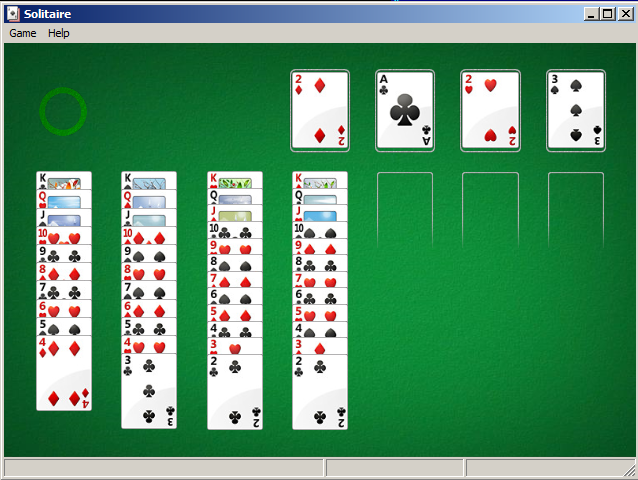
\includegraphics[width=0.6\textwidth]{examples/lines/1.png}
\caption{Ceci est l'allure du jeu en général}
\label{fig:lines_1}
\end{figure}

\clearpage
\myindex{\CStandardLibrary!rand()}

Dons regardons s'il est possible de trouver le générateur d'aléas et de jouer des tours avec.
\IDA reconnaît rapidement la fonction standard \TT{\_rand} dans \TT{balltrix.exe} en \TT{0x00403DA0}.
\IDA montre aussi qu'elle n'est appelée que d'un seul endroit:

\lstinputlisting[style=customasmx86]{examples/lines/random.lst}

Appelons-la \q{random}.
Ne plongeons pas encore dans le code de cette fonction.

Cette fonction est référencée depuis 3 endroits.

Voici les deux premiers:

\lstinputlisting[style=customasmx86]{examples/lines/1.lst}

Voici le troisième:

\lstinputlisting[style=customasmx86]{examples/lines/2.lst}

Donc la fonction n'a qu'un argument.

10 est passé dans les deux premiers cas et 5 dans le troisième.
Nous pouvons aussi remarquer que le plateau a une taille de 10*10, et qu'il y a 5
couleurs possible.
C'est ça!
La fonction standard \TT{rand()} renvoie un nombre dans l'intervalle \TT{0..0x7FFF}
et c'est souvent peu pratique, donc beaucoup de programmeurs implémentent leur propre
fonction qui renvoie un nombre aléatoire dans un intervalle spécifié.
Dans notre cas, l'intervalle est $0..n-1$ et $n$ est passé comme unique argument
à la fonction.
Nous pouvons tester cela rapidement dans le débogueur.

Donc modifions le troisième appel de la fonction, afin qu'il renvoie toujours zéro.
Premièrement, nous allons remplacer trois instructions (\TT{PUSH/CALL/ADD}) par des \ac{NOP}s.
Puis, nous allons ajouter l'instruction \INS{XOR EAX, EAX} pour effacer le registre
\EAX.

\lstinputlisting[style=customasmx86]{examples/lines/fixed.lst}

Nous avons remplacé l'appel à la fonction \TT{random()} par du code qui renvoie toujours
zéro.

\clearpage
Lançons-le maintenant:

\begin{figure}[H]
\centering
\includegraphics[width=0.6\textwidth]{examples/lines/2.png}
\caption{La blague fonctionne}
\end{figure}

Hé oui, ça fonctionne\footnote{J'ai fait une fois cette blague à des collègues dans
l'espoir qu'ils arrêtent de jouer. Mais ça n'a pas fonctionné.}.

Mais pourquoi est-ce que les arguments de la fonction \TT{random()} sont des variables
globales?
C'est seulement parce qu'il est possible de changer la taille du plateau dans les
préférences du jeu, donc ces valeurs ne sont pas codées en dur.
Le valeurs 10 et 5 sont celles par défaut.

\mysection{\MinesweeperWinXPExampleChapterName}
\label{minesweeper_winxp}
\myindex{Windows!Windows XP}

Pour ceux qui ne sont pas très bons avec le jeu démineur, nous pouvons essayer de
révéler les mines cachées dans le débogueur.

\myindex{\CStandardLibrary!rand()}
\myindex{Windows!PDB}

Comme on le sait, le démineur place des mines aléatoirement, donc il doit y avoir
une sorte de générateur de nombre aléatoire ou un appel à la fonction C standard
\TT{rand()}.

Ce qui est vraiment cool en rétro-ingénierant des produits Microsoft c'est qu'il
y a les fichiers \gls{PDB} avec les symboles (nom de fonctions, etc.)
Lorsque nous chargeons \TT{winmine.exe} dans \IDA, il télécharge le fichier \gls{PDB}
exact pour cet exécutable et affiche tous les noms.

Donc le voici, le seul appel à \TT{rand()} est cette fonction:

\lstinputlisting[style=customasmx86]{examples/minesweeper/tmp1.lst}

\IDA l'a appelé ainsi, et c'est le nom que lui ont donné les développeurs du démineur.

La fonction est très simple:

\begin{lstlisting}[style=customc]
int Rnd(int limit)
{
    return rand() % limit;
};
\end{lstlisting}

(Il n'y a pas de nom \q{limit} dans le fichier \gls{PDB}; nous avons nommé manuellement
les arguments comme ceci.)

Donc elle renvoie une valeur aléatoire entre 0 et la limite spécifiée.

\TT{Rnd()} est appelée depuis un seul endroit, la fonction appelée \TT{StartGame()},
et il semble bien que ce soit exactement le code qui place les mines:

\begin{lstlisting}[style=customasmx86]
.text:010036C7                 push    _xBoxMac
.text:010036CD                 call    _Rnd@4          ; Rnd(x)
.text:010036D2                 push    _yBoxMac
.text:010036D8                 mov     esi, eax
.text:010036DA                 inc     esi
.text:010036DB                 call    _Rnd@4          ; Rnd(x)
.text:010036E0                 inc     eax
.text:010036E1                 mov     ecx, eax
.text:010036E3                 shl     ecx, 5          ; ECX=ECX*32
.text:010036E6                 test    _rgBlk[ecx+esi], 80h
.text:010036EE                 jnz     short loc_10036C7
.text:010036F0                 shl     eax, 5          ; EAX=EAX*32
.text:010036F3                 lea     eax, _rgBlk[eax+esi]
.text:010036FA                 or      byte ptr [eax], 80h
.text:010036FD                 dec     _cBombStart
.text:01003703                 jnz     short loc_10036C7
\end{lstlisting}

Le démineur vous permet de définir la taille du plateau, donc les dimensions X (xBoxMac)
et Y (yBoxMac) du plateau sont des variables globales.
Elles sont passées à \TT{Rnd()} et des coordonnées aléatoires sont générées.
Une mine est placée par l'instruction \TT{OR} en \TT{0x010036FA}.
Et si une mine y a déjà été placée avant (il est possible que la fonction \TT{Rnd()}
génère une paire de coordonnées qui a déjà été générée), alors les instructions \TT{TEST}
et \TT{JNZ} en \TT{0x010036E6} bouclent sur la routine de génération.

\TT{cBombStart} est la variable globale contenant le nombre total de mines. Donc
ceci est une boucle.

La largeur du tableau est 32 (nous pouvons conclure ceci en regardant l'instruction
\TT{SHL}, qui multiplie l'une des coordonnées par 32).

La taille du tableau global \TT{rgBlk} peut facilement être déduite par la différence
entre le label \TT{rgBlk} dans le segment de données et le label suivant. Il s'agit
de 0x360 (864):

\begin{lstlisting}[style=customasmx86]
.data:01005340 _rgBlk          db 360h dup(?)          ; DATA XREF: MainWndProc(x,x,x,x)+574
.data:01005340                                         ; DisplayBlk(x,x)+23
.data:010056A0 _Preferences    dd ?                    ; DATA XREF: FixMenus()+2
...
\end{lstlisting}

$864/32=27$.

Donc, la taille du tableau est-elle $27*32$?
C'est proche de ce que nous savons: lorsque nous essayons de définir la taille du
plateau à $100*100$ dans les préférences du démineur, il corrige à une taille de
plateau de $24*30$.
Donc ceci est la taille maximale du plateau.
Et le tableau a une taille fixe, pour toutes les tailles de plateau.

REgardons tout ceci dans \olly.
Nous allons lancer le démineur, lui attacher \olly et nous allons pouvoir voir le
contenu de la mémoire à l'adresse du tableau \TT{rgBlk} (\TT{0x01005340})\footnote{Toutes
les adresses ici sont pour le démineur de Windows XP SP3 English. Elles peuvent être
différentes pour d'autres services packs.}.
Donc nous avons ceci à l'emplacement mémoire du tableau:

\lstinputlisting[style=customasmx86]{examples/minesweeper/1.lst}

\olly, comme tout autre éditeur hexadécimal, affiche 16 octets par ligne.
Donc chaque ligne de tableau de 32-octet occupe exactement 2 lignes ici.

Ceci est le niveau débutant (plateau de 9*9).

Il y a une sorte de structure carré que l'on voit ici (octets 0x10).

Nous cliquons \q{Run} dans \olly pour débloquer le processus du démineur, puis nous
cliquons au hasard dans la fenêtre du démineur et nous tombons sur une mine, mais
maintenant, toutes les mines sont visibles:

\begin{figure}[H]
\centering
\myincludegraphicsSmall{examples/minesweeper/1.png}
\caption{Mines}
\label{fig:minesweeper1}
\end{figure}

En comparant les emplacements des mines et le dump, nous pouvons en conclure que
0x10 correspond au bord, 0x0F---bloc vide, 0x8F---mine.
Peut-être que 0x10 est simplement une \emph{valeur sentinelle}.

Maintenant nous allons ajouter des commentaires et aussi mettre tous les octets à
0x8F entre parenthèses droites:

\lstinputlisting[style=customasmx86]{examples/minesweeper/2.lst}

Maintenant nous allons supprimer tous les \emph{octet de bord} (0x10) et ce qu'il
y a après:

\lstinputlisting[style=customasmx86]{examples/minesweeper/3.lst}

Oui, ce sont des mines, maintenant ça peut être vu clairement et comparé avec la
copie d'écran.

\clearpage
Ce qui est intéressant, c'est que nous pouvons modifier le tableau directement dans
\olly.
Nous pouvons supprimer toutes les mines en changeant les octets à 0x8F par 0x0F,
et voici ce que nous obtenons dans le démineur:

\begin{figure}[H]
\centering
\myincludegraphicsSmall{examples/minesweeper/3.png}
\caption{Toutes les mines sont supprimées depuis le débogueur}
\label{fig:minesweeper3}
\end{figure}

Nous pouvons aussi toutes les déplacer à la première ligne:

\begin{figure}[H]
\centering
\myincludegraphicsSmall{examples/minesweeper/2.png}
\caption{Mines mises dans le débogueur}
\label{fig:minesweeper2}
\end{figure}

Bon, le débogueur n'est pas très pratique pour espionner (ce qui est notre but),
donc nous allons écrire un petit utilitaire pour afficher le contenu du plateau:

\lstinputlisting[style=customc]{examples/minesweeper/minesweeper_cheater.c}

Simplement donner le \ac{PID}
\footnote{Le PID peut être vu dans le Task Manager
(l'activer avec \q{View $\rightarrow$ Select Columns})}
et l'adresse du tableau (\TT{0x01005340} pour Windows XP SP3 English)
et il l'affichera
\footnote{L'exécutable compilé est ici:
\href{http://go.yurichev.com/17165}{beginners.re}}.

Il s'attache à un processus win32 par le \ac{PID} et lit la mémoire du processus
à l'adresse.

\subsection{Trouver la grille automatiquement}

C'est pénible de mettre l'adresse à chaque fois que nous lançons notre utilitaire.
Aussi, différentes versions du démineur peuvent avoir le tableau à des adresses différentes.
Sachant qu'il a toujours un bord (octets 0x10), nous pouvons le trouver facilement
en mémoire:

\lstinputlisting[style=customc]{examples/minesweeper/cheater2_fragment.c}

Code source complet: \url{\RepoURL/examples/minesweeper/minesweeper_cheater2.c}.

\subsection{\Exercises}

\begin{itemize}

\item 
Pourquoi est-ce que les \emph{octets de bord} (ou \emph{valeurs sentinelles}) (0x10)
existent dans le tableau?

À quoi servent-elles si elles ne sont pas visibles dans l'interface du démineur?
Comment est-ce qu'il pourrait fonctionner sans elles?

\item 
Comme on s'en doute, il y a plus de valeurs possible (pour les blocs ouverts, ceux
flagués par l'utilisateur, etc.).
Essayez de trouver la signification de chacune d'elles.

\item 
Modifiez mon utilitaire afin qu'il puisse supprimer toutes les mines ou qu'il les
place suivant un schéma fixé de votre choix dans le démineur.

\end{itemize}

\mysection{Hacker l'horloge de Windows}

Parfois je fais des poissons d'avril à mes collègues.

Cherchons si nous pourrions faire quelque chose avec l'horloge de Windows?
Pouvons-nous la forcer à tourner à l'envers?

Tout d'abord, lorsque l'on clique sur date/time dans la barre d'état,\\
le module \emph{C:\textbackslash{}WINDOWS\textbackslash{}SYSTEM32\textbackslash{}TIMEDATE.CPL}
est exécuté, qui est un fichier exécutable \ac{PE} habituel.

Voyons d'abord comment il affiche les aiguilles.
Lorsque j'ouvre le fichier (de Windows 7) dans Resource Hacker, il y a le fond de
l'horloge, mais sans aiguille:

\begin{figure}[H]
\centering
\myincludegraphics{examples/timedate/reshack.png}
\caption{Resource Hacker}
\end{figure}

Ok, que savons-nous? Comment afficher une aiguille? Elles commencent au milieu du
cercle, s'arrêtent sur son bord.
De ce fait, nous devons calculer les coordonnées d'un point sur le bord d'un cercle.
Des mathématiques scolaires, nous pouvons nous rappeler que nous devons utiliser
les fonctions sinus/cosinus pour dessiner un cercle, ou au moins la racine carré.
Il n'y a pas de telles choses dans \emph{TIMEDATE.CPL}, au moins à première vue.
Mais grâce au fichier PDB de débogage de Microsoft, je peux trouver une fonction
appelée \emph{CAnalogClock::DrawHand()}, qui appelle \emph{Gdiplus::Graphics::DrawLine()}
au moins deux fois.

Voici le code:

\lstinputlisting[style=customasmx86]{examples/timedate/1.lst}

\myindex{Windows!Win32!MulDiv()}
Nous voyons que les arguments de \emph{DrawLine()} dépendent du résultat de la fonction
\emph{MulDiv()} et d'une table \emph{table[]} (le nom est mien), qui a des éléments
de 8-octets (regardez le second opérande de \INS{LEA}).

Qu'y a-t-il dans table[]?

\lstinputlisting[style=customasmx86]{examples/timedate/2.lst}

Elle n'est référencée que depuis la fonction \emph{DrawHand()}.
Elle a 120 mots de 32-bit ou 60 paires 32-bit... attendez, 60?
Regardons ces valeurs de plus près.
Tout d'abord, je vais remplacer 6 paires ou 12 mots de 32-bit par des zéros, et je
vais mettre le fichier \emph{TIMEDATE.CPL} modifié dans \emph{C:\textbackslash{}WINDOWS\textbackslash{}SYSTEM32}.
(Vous pourriez devoir changer le propriétaire du fichier *TIMEDATE.CPL* pour votre
compte utilisateur primaire (au lieu de \emph{TrustedInstaller}), et donc, démarrer
en mode sans échec avec la ligne de commande afin de pouvoir copier le fichier, qui
est en général bloqué.)

\begin{figure}[H]
\centering
\includegraphics[width=0.5\textwidth]{examples/timedate/6_pairs_zeroed.png}
\caption{Tentative d'exécution}
\end{figure}

Maintenant lorsqu'une aiguilles est située dans 0..5 secondes/minutes, elle est invisible!
Toutefois, la partie opposée (plus courte) de la seconde aiguille est visible et
bouge.
Lorsqu'une aiguille est en dehors de cette partie, elle est visible comme d'habitude.

\myindex{Mathematica}
Regardons d' encore plus près la table dans Mathematica.
J'ai copié/collé la table de \emph{TIMEDATE.CPL} dans un fichier \emph{tbl} (480 octets).
Nous tenons pour acquis le fait que ce sont des valeurs signées, car la moitié des
éléments sont inférieurs à zéro (0FFFFE0C1h, etc.).
Si ces valeurs étaient non signées, elles seraient étrangement grandes.

\begin{lstlisting}[style=custommath]
In[]:= tbl = BinaryReadList["~/.../tbl", "Integer32"]

Out[]= {0, -7999, 836, -7956, 1663, -7825, 2472, -7608, 3253, -7308, 3999, \
-6928, 4702, -6472, 5353, -5945, 5945, -5353, 6472, -4702, 6928, \
-4000, 7308, -3253, 7608, -2472, 7825, -1663, 7956, -836, 8000, 0, \
7956, 836, 7825, 1663, 7608, 2472, 7308, 3253, 6928, 4000, 6472, \
4702, 5945, 5353, 5353, 5945, 4702, 6472, 3999, 6928, 3253, 7308, \
2472, 7608, 1663, 7825, 836, 7956, 0, 7999, -836, 7956, -1663, 7825, \
-2472, 7608, -3253, 7308, -4000, 6928, -4702, 6472, -5353, 5945, \
-5945, 5353, -6472, 4702, -6928, 3999, -7308, 3253, -7608, 2472, \
-7825, 1663, -7956, 836, -7999, 0, -7956, -836, -7825, -1663, -7608, \
-2472, -7308, -3253, -6928, -4000, -6472, -4702, -5945, -5353, -5353, \
-5945, -4702, -6472, -3999, -6928, -3253, -7308, -2472, -7608, -1663, \
-7825, -836, -7956}

In[]:= Length[tbl]
Out[]= 120
\end{lstlisting}

Traitons deux valeurs consécutives comme une paire:

\begin{lstlisting}[style=custommath]
In[]:= pairs = Partition[tbl, 2]
Out[]= {{0, -7999}, {836, -7956}, {1663, -7825}, {2472, -7608}, \
{3253, -7308}, {3999, -6928}, {4702, -6472}, {5353, -5945}, {5945, \
-5353}, {6472, -4702}, {6928, -4000}, {7308, -3253}, {7608, -2472}, \
{7825, -1663}, {7956, -836}, {8000, 0}, {7956, 836}, {7825, 
1663}, {7608, 2472}, {7308, 3253}, {6928, 4000}, {6472, 
4702}, {5945, 5353}, {5353, 5945}, {4702, 6472}, {3999, 
6928}, {3253, 7308}, {2472, 7608}, {1663, 7825}, {836, 7956}, {0, 
7999}, {-836, 7956}, {-1663, 7825}, {-2472, 7608}, {-3253, 
7308}, {-4000, 6928}, {-4702, 6472}, {-5353, 5945}, {-5945, 
5353}, {-6472, 4702}, {-6928, 3999}, {-7308, 3253}, {-7608, 
2472}, {-7825, 1663}, {-7956, 836}, {-7999, 
0}, {-7956, -836}, {-7825, -1663}, {-7608, -2472}, {-7308, -3253}, \
{-6928, -4000}, {-6472, -4702}, {-5945, -5353}, {-5353, -5945}, \
{-4702, -6472}, {-3999, -6928}, {-3253, -7308}, {-2472, -7608}, \
{-1663, -7825}, {-836, -7956}}

In[]:= Length[pairs]
Out[]= 60
\end{lstlisting}

Essayons de traiter chaque paire comme des coordonnées X/Y et dessinons les 60 paires,
et aussi les 15 premières paires:

\begin{figure}[H]
\centering
\myincludegraphics{examples/timedate/math.png}
\caption{Mathematica}
\end{figure}

Ça donne quelque chose!
Chaque paire est juste une coordonnée.
Les 15 premières paires sont les coordonnées pour $\frac{1}{4}$ de cercle.

Peut-être que les développeurs de Microsoft ont pré-calculé toutes les coordonnées
et les ont mises dans une table.
myindex{Memoization}
Ceci est une pratique très répandue, quoique désuète -- l'accès à une table précalculée
est plus rapide que d'appeler les fonctions sinus/cosinus relativement lente\footnote{Aujourd'hui
ceci est appelé la \emph{memoïsation}}.
Les opérations sinus/cosinus ne sont plus aussi couteuses...

Maintenant, je comprends pourquoi lorsque j'ai effacé les 6 premières paires, les
aiguilles étaient invisibles dans cette zone: en fait, les aiguilles étaient dessinées,
elles avaient juste une longueur de zéro, car elles commençaient et finissaient en (0,0).

\subsubsection{La blague}

Sachant tout cela, comment serait-il possible de forcer les aiguilles à tourner à
l'envers?
En fait, ceci est simple, nous devons seulement tourner la table, afin que chaque
aiguille, au lieu d'être dessinée à l'index 0, le soit à l'index 59.

J'ai créé le modificateur il y a longtemps, au tout début des années 2000, pour Windows 2000.
Difficile à croire, il fonctionne toujours pour Windows 7, peut-être que la table
n'a pas changé depuis lors!

Code source du modificateur: \url{\RepoURL/examples/timedate/time_pt.c}.

Maintenant, je peux voir les aiguilles tourner à l'envers:

\begin{figure}[H]
\centering
\includegraphics[width=0.5\textwidth]{examples/timedate/counterclockwise.png}
\caption{Maintenant ça fonctionne}
\end{figure}

Bon, il n'y a pas d'animation dans ce livre, mais si vous y regardez de plus près,
vous pouvez voir que les aiguilles affichent en fait l'heure correcte, mais que la
surface entière de l'horloge est tournée verticalement, comme si nous la voyons depuis
l'intérieur de l'horloge.

\subsubsection{Code source divulgué de Windows 2000}

Donc, j'ai écrit le modificateur et ensuite le code source de Windows 2000 a fuité
(je ne peux toutefois pas vous obligez à me croire).
Jettons un coup d'\oe{}il au code source de cette fonction et à la table.\\
Le fichier est \emph{win2k/private/shell/cpls/utc/clock.c}:

\begin{lstlisting}[style=customc]
//
//  Array containing the sine and cosine values for hand positions.
//
POINT rCircleTable[] =
{
    { 0,     -7999},
    { 836,   -7956},
    { 1663,  -7825},
    { 2472,  -7608},
    { 3253,  -7308},
...
    { -4702, -6472},
    { -3999, -6928},
    { -3253, -7308},
    { -2472, -7608},
    { -1663, -7825},
    { -836 , -7956},
};

////////////////////////////////////////////////////////////////////////////
//
//  DrawHand
//
//  Draws the hands of the clock.
//
////////////////////////////////////////////////////////////////////////////

void DrawHand(
    HDC hDC,
    int pos,
    HPEN hPen,
    int scale,
    int patMode,
    PCLOCKSTR np)
{
    LPPOINT lppt;
    int radius;

    MoveTo(hDC, np->clockCenter.x, np->clockCenter.y);
    radius = MulDiv(np->clockRadius, scale, 100);
    lppt = rCircleTable + pos;
    SetROP2(hDC, patMode);
    SelectObject(hDC, hPen);

    LineTo( hDC,
            np->clockCenter.x + MulDiv(lppt->x, radius, 8000),
            np->clockCenter.y + MulDiv(lppt->y, radius, 8000) );
}
\end{lstlisting}

Maintenant, c'est clair: les coordonnées sont pré-calculées comme si la surface de
l'horloge avait une hauteur et une largeur de $2 \cdot 8000$, et ensuite elles sont
adaptées au rayon actuel de l'horloge en utilisant la fonction \emph{MulDiv()}.

La structure POINT\footnote{\url{https://msdn.microsoft.com/en-us/library/windows/desktop/dd162805(v=vs.85).aspx}}
est une structure de deux valeurs 32-bit, la première est \emph{x}, la seconde \emph{y}.


\mysection{Solitaire (Windows 7): blagues}

\input{examples/solitaire/51/main_FR}
\input{examples/solitaire/53/main_FR}


\subsection{Table \TT{X\$KSMLRU} dans \oracle}
\myindex{\oracle}

Il y a une mention d'une table spéciale dans la note \emph{Diagnosing and Resolving
Error ORA-04031 on the Shared Pool or Other Memory Pools [Video] [ID 146599.1]}:

\begin{framed}
\begin{quotation}
Il y a une table fixée appelée X\$KSMLRU qui suit les différentes allocations dans
le pool partagé qui force les autres objets du pool partagé à vieillir. Cette table
fixée peut être utilisée pour identifier ce qui cause une grosse allocation.

Si plusieurs objets sont supprimés périodiquement du pool partagé, alors ceci va poser des problèmes de temps de réponse
et va probablement provoquer des problèmes de contention du verrou de cache de bibliothèque lorsque
les objets seront rechargés dans le pool partagé.

Une chose inhabituelle à propos de la table fixée X\$KSMLRU est que le contenu de la table fixée est écrasé à chaque fois que
quelqu'uni effectue requête dans la table fixée. Ceci est fait puisque la table fixée ne contient que l'allocation la plus large
qui s'est produite. Les valeurs sont réinitialisées après avoir été sélectionnées, de sorte que les allocations importantes
suivantes puissent ête inscrites, même si elles ne sont pas aussi laarges que celles qui se sont produites précédemment.
À cause de cette réinitialisation, la sortie produite par la sélection de cette table doit être soigneusement conservée
puisqu'elle ne peut plus être récupérée après que la requête a été faite.
\end{quotation}
\end{framed}

Toutefois, comme on peut le vérifier facilement, le contenu de cette table est effacé à chaque fois qu'on l'interroge.
Pouvons-nous trouver pourquoi?
Retournons aux tables que nous connaissons déjà: \TT{kqftab} et \TT{kqftap} qui
sont générées avec l'aide d'\oracletables, qui a toutes les informations concernant les table X\$-.
Nous pouvons voir ici que la fonction \TT{ksmlrs()} est appelée pour préparer les éléments de cette table:

\begin{lstlisting}[caption=Résultat de \OracleTablesName]
kqftab_element.name: [X$KSMLRU] ?: [ksmlr] 0x4 0x64 0x11 0xc 0xffffc0bb 0x5
kqftap_param.name=[ADDR] ?: 0x917 0x0 0x0 0x0 0x4 0x0 0x0
kqftap_param.name=[INDX] ?: 0xb02 0x0 0x0 0x0 0x4 0x0 0x0
kqftap_param.name=[INST_ID] ?: 0xb02 0x0 0x0 0x0 0x4 0x0 0x0
kqftap_param.name=[KSMLRIDX] ?: 0xb02 0x0 0x0 0x0 0x4 0x0 0x0
kqftap_param.name=[KSMLRDUR] ?: 0xb02 0x0 0x0 0x0 0x4 0x4 0x0
kqftap_param.name=[KSMLRSHRPOOL] ?: 0xb02 0x0 0x0 0x0 0x4 0x8 0x0
kqftap_param.name=[KSMLRCOM] ?: 0x501 0x0 0x0 0x0 0x14 0xc 0x0
kqftap_param.name=[KSMLRSIZ] ?: 0x2 0x0 0x0 0x0 0x4 0x20 0x0
kqftap_param.name=[KSMLRNUM] ?: 0x2 0x0 0x0 0x0 0x4 0x24 0x0
kqftap_param.name=[KSMLRHON] ?: 0x501 0x0 0x0 0x0 0x20 0x28 0x0
kqftap_param.name=[KSMLROHV] ?: 0xb02 0x0 0x0 0x0 0x4 0x48 0x0
kqftap_param.name=[KSMLRSES] ?: 0x17 0x0 0x0 0x0 0x4 0x4c 0x0
kqftap_param.name=[KSMLRADU] ?: 0x2 0x0 0x0 0x0 0x4 0x50 0x0
kqftap_param.name=[KSMLRNID] ?: 0x2 0x0 0x0 0x0 0x4 0x54 0x0
kqftap_param.name=[KSMLRNSD] ?: 0x2 0x0 0x0 0x0 0x4 0x58 0x0
kqftap_param.name=[KSMLRNCD] ?: 0x2 0x0 0x0 0x0 0x4 0x5c 0x0
kqftap_param.name=[KSMLRNED] ?: 0x2 0x0 0x0 0x0 0x4 0x60 0x0
kqftap_element.fn1=ksmlrs
kqftap_element.fn2=NULL
\end{lstlisting}

\myindex{tracer}
En effet, avec l'aide de \tracer, il est facile de voir que cette fonction est appelée
à chaque fois que nous interrogeons la table \TT{X\$KSMLRU}.

\myindex{\CStandardLibrary!memset()}
Ici nous voyons une référence aux fonctions \TT{ksmsplu\_sp()} et \TT{ksmsplu\_jp()},
chacune d'elles appelle \TT{ksmsplu()} à la fin.
À la fin de la fonction \TT{ksmsplu()} nous voyons un appel à \TT{memset()}:

\begin{lstlisting}[caption=ksm.o,style=customasmx86]
...

.text:00434C50 loc_434C50:    ; DATA XREF: .rdata:off\_5E50EA8
.text:00434C50         mov     edx, [ebp-4]
.text:00434C53         mov     [eax], esi
.text:00434C55         mov     esi, [edi]
.text:00434C57         mov     [eax+4], esi
.text:00434C5A         mov     [edi], eax
.text:00434C5C         add     edx, 1
.text:00434C5F         mov     [ebp-4], edx
.text:00434C62         jnz     loc_434B7D
.text:00434C68         mov     ecx, [ebp+14h]
.text:00434C6B         mov     ebx, [ebp-10h]
.text:00434C6E         mov     esi, [ebp-0Ch]
.text:00434C71         mov     edi, [ebp-8]
.text:00434C74         lea     eax, [ecx+8Ch]
.text:00434C7A         push    370h            ; Size
.text:00434C7F         push    0               ; Val
.text:00434C81         push    eax             ; Dst
.text:00434C82         call    __intel_fast_memset
.text:00434C87         add     esp, 0Ch
.text:00434C8A         mov     esp, ebp
.text:00434C8C         pop     ebp
.text:00434C8D         retn
.text:00434C8D _ksmsplu  endp
\end{lstlisting}

Des constructions comme \TT{memset (block, 0, size)} sont souvent utilisées pour
mettre à zéro un bloc de mémoire.
Que se passe-t-il si nous prenons le risque de bloquer l'appel à \TT{memset (block, 0, size)}
et regardons ce qui se produit?

\myindex{tracer}

Lançons \tracer avec les options suivantes: mettre un point d'arrêt en \TT{0x434C7A}
(le point où les arguments sont passés à \TT{memset()}), afin que \tracer mette le compteur de programme \TT{EIP} au point
où les arguments passés à \TT{memset()} sont éffacés (en \TT{0x434C8A}).
On peut dire que nous simulons juste un saut inconditionnel de l'adresse \TT{0x434C7A} à \TT{0x434C8A}.

\begin{lstlisting}
tracer -a:oracle.exe bpx=oracle.exe!0x00434C7A,set(eip,0x00434C8A)
\end{lstlisting}

(Important: toutes ces adresses sont valides seulement pour la version win32 de \oracle 11.2)

En effet, nous pouvons maintenant interroger la table \TT{X\$KSMLRU} autant de fois
que nous voulons et elle n'est plus du tout effacée!

% \sout{Do not try this at home ("MythBusters")}
Au cas où, n'essayez pas ceci sur vos serveurs de production.

Ce n'est probablement pas un comportement très utile ou souhaité, mais comme une
expérience pour déterminer l'emplacement d'un bout de code dont nous avons besoin,
ça remplit parfaitement notre besoin!


\mysection{\q{QR9}: algorithme cryptographique amateur inspiré du Rubik's cube}

Parfois, les systèmes cryptographiques amateurs sont assez bizarres.

On m'a demandé une fois de rétro-ingénieurer un algorithme cryptographique amateur
d'un utilitaire de chiffrement, dont le code source avait été perdu\footnote{J'ai
aussi reçu la permission du client de publier les détails de l'algorithme.}.

Voici le listing exporté depuis \IDA de l'utilitaire de chiffrement d'origine:


Tous les noms de fonction et de label ont été donné par moi lors de l'analyse.

Commençons depuis le haut. Voici une fonction qui prend deux noms de fichier et un
mot de passe.

\begin{lstlisting}[style=customasmx86]
.text:00541320 ; int \_\_cdecl crypt\_file(char *Str, char *Filename, int password)
.text:00541320 crypt_file      proc near
.text:00541320
.text:00541320 Str             = dword ptr  4
.text:00541320 Filename        = dword ptr  8
.text:00541320 password        = dword ptr  0Ch
.text:00541320
\end{lstlisting}

Ouvrir le fichier et signaler si une erreur survient:

\begin{lstlisting}[style=customasmx86]
.text:00541320                 mov     eax, [esp+Str]
.text:00541324                 push    ebp
.text:00541325                 push    offset Mode     ; "rb"
.text:0054132A                 push    eax             ; Str
.text:0054132B                 call    _fopen          ; ouvrir le fichier
.text:00541330                 mov     ebp, eax
.text:00541332                 add     esp, 8
.text:00541335                 test    ebp, ebp
.text:00541337                 jnz     short loc_541348
.text:00541339                 push    offset Format   ; "Cannot open input file!\\n"
.text:0054133E                 call    _printf
.text:00541343                 add     esp, 4
.text:00541346                 pop     ebp
.text:00541347                 retn
.text:00541348
.text:00541348 loc_541348:
\end{lstlisting}

\myindex{\CStandardLibrary!fseek()}
\myindex{\CStandardLibrary!ftell()}
Obtenir la taille du fichier via \TT{fseek()}/\TT{ftell()}:

\lstinputlisting[style=customasmx86]{examples/qr9/1_FR}

Ce morceau de code calcule la taille du fichier aligné sur une limite de 64-octet.
Ceci car l'algorithme cryptographique travaille seulement avec des blocs de 64 octets.
L'opération est assez directe: diviser la taille du fichier par 64, ignorer le reste
et ajouter 1, puis, multiplier par 64.
Le code suivant enlève le reste comme si la valeur avait déjà été divisée par 64
et ajoute 64.

\lstinputlisting[style=customasmx86]{examples/qr9/2_FR}

Alloue le buffer avec une taille alignée:

\begin{lstlisting}[style=customasmx86]
.text:00541373                 push    esi             ; Size
.text:00541374                 call    _malloc
\end{lstlisting}

\myindex{\CStandardLibrary!calloc()}
Appelle memset(), p. ex., efface le buffer alloué\footnote{malloc() + memset() pourraient
être remplacés par calloc().}.

\lstinputlisting[style=customasmx86]{examples/qr9/3_FR}

Lit le fichier via la fonction C standard \TT{fread()}.

\begin{lstlisting}[style=customasmx86]
.text:00541392                 mov     eax, [esp+38h+Str]
.text:00541396                 push    eax             ; ElementSize
.text:00541397                 push    ebx             ; DstBuf
.text:00541398                 call    _fread          ; lire le fichier
.text:0054139D                 push    ebp             ; File
.text:0054139E                 call    _fclose
\end{lstlisting}

Appelle \TT{crypt()}. Cette fonction prend un buffer, sa taille (alignée) et une chaîne
mot de passe.

\begin{lstlisting}[style=customasmx86]
.text:005413A3                 mov     ecx, [esp+44h+password]
.text:005413A7                 push    ecx             ; mot de passe
.text:005413A8                 push    esi             ; aligner la taille
.text:005413A9                 push    ebx             ; buffer
.text:005413AA                 call    crypt           ; chiffrer
\end{lstlisting}

Crée le fichier de sortie. À propos, le développeur a oublié de vérifier s'il a été
créé correctement!

\begin{lstlisting}[style=customasmx86]
.text:005413AF                 mov     edx, [esp+50h+Filename]
.text:005413B3                 add     esp, 40h
.text:005413B6                 push    offset aWb      ; "wb"
.text:005413BB                 push    edx             ; Filename
.text:005413BC                 call    _fopen
.text:005413C1                 mov     edi, eax
\end{lstlisting}

Le handle du fichier nouvellement créé est maintenant dans le registre \EDI. Écrit
la signature \q{QR9}.

\begin{lstlisting}[style=customasmx86]
.text:005413C3                 push    edi             ; File
.text:005413C4                 push    1               ; Count
.text:005413C6                 push    3               ; Size
.text:005413C8                 push    offset aQr9     ; "QR9"
.text:005413CD                 call    _fwrite         ; écrire la signature du fichier
\end{lstlisting}

Écrit la taille réelle du fichier (non alignée):

\begin{lstlisting}[style=customasmx86]
.text:005413D2                 push    edi             ; File
.text:005413D3                 push    1               ; Count
.text:005413D5                 lea     eax, [esp+30h+Str]
.text:005413D9                 push    4               ; Size
.text:005413DB                 push    eax             ; Str
.text:005413DC                 call    _fwrite         ; écrire la taille du fichier original
\end{lstlisting}

Écrit le buffer chiffré:

\begin{lstlisting}[style=customasmx86]
.text:005413E1                 push    edi             ; File
.text:005413E2                 push    1               ; Count
.text:005413E4                 push    esi             ; Size
.text:005413E5                 push    ebx             ; Str
.text:005413E6                 call    _fwrite         ; écrire le fichier chiffré
\end{lstlisting}

Ferme le fichier et libère le buffer alloué:

\begin{lstlisting}[style=customasmx86]
.text:005413EB                 push    edi             ; File
.text:005413EC                 call    _fclose
.text:005413F1                 push    ebx             ; Memory
.text:005413F2                 call    _free
.text:005413F7                 add     esp, 40h
.text:005413FA                 pop     edi
.text:005413FB                 pop     esi
.text:005413FC                 pop     ebx
.text:005413FD                 pop     ebp
.text:005413FE                 retn
.text:005413FE crypt_file      endp
\end{lstlisting}

Voici le code C reconstruit:

\begin{lstlisting}[style=customc]
void crypt_file(char *fin, char* fout, char *pw)
{
	FILE *f;
	int flen, flen_aligned;
	BYTE *buf;

	f=fopen(fin, "rb");
	
	if (f==NULL)
	{
		printf ("Cannot open input file!\n");
		return;
	};

	fseek (f, 0, SEEK_FRD);
	flen=ftell (f);
	fseek (f, 0, SEEK_SET);

	flen_aligned=(flen&0xFFFFFFC0)+0x40;

	buf=(BYTE*)malloc (flen\_aligned);
	memset (buf, 0, flen\_aligned);

	fread (buf, flen, 1, f);

	fclose (f);

	crypt (buf, flen\_aligned, pw);
	
	f=fopen(fout, "wb");

	fwrite ("QR9", 3, 1, f);
	fwrite (&flen, 4, 1, f);
	fwrite (buf, flen\_aligned, 1, f);

	fclose (f);

	free (buf);
};
\end{lstlisting}

La procédure de déchiffrement est presque la même:

\begin{lstlisting}[style=customasmx86]
.text:00541400 ; int \_\_cdecl decrypt\_file(char *Filename, int, void *Src)
.text:00541400 decrypt_file    proc near
.text:00541400
.text:00541400 Filename        = dword ptr  4
.text:00541400 arg_4           = dword ptr  8
.text:00541400 Src             = dword ptr  0Ch
.text:00541400
.text:00541400                 mov     eax, [esp+Filename]
.text:00541404                 push    ebx
.text:00541405                 push    ebp
.text:00541406                 push    esi
.text:00541407                 push    edi
.text:00541408                 push    offset aRb      ; "rb"
.text:0054140D                 push    eax             ; Filename
.text:0054140E                 call    _fopen
.text:00541413                 mov     esi, eax
.text:00541415                 add     esp, 8
.text:00541418                 test    esi, esi
.text:0054141A                 jnz     short loc_54142E
.text:0054141C                 push    offset aCannotOpenIn_0 ; "Cannot open input file!\\n"
.text:00541421                 call    _printf
.text:00541426                 add     esp, 4
.text:00541429                 pop     edi
.text:0054142A                 pop     esi
.text:0054142B                 pop     ebp
.text:0054142C                 pop     ebx
.text:0054142D                 retn
.text:0054142E
.text:0054142E loc_54142E:
.text:0054142E                 push    2               ; Origin
.text:00541430                 push    0               ; Offset
.text:00541432                 push    esi             ; File
.text:00541433                 call    _fseek
.text:00541438                 push    esi             ; File
.text:00541439                 call    _ftell
.text:0054143E                 push    0               ; Origin
.text:00541440                 push    0               ; Offset
.text:00541442                 push    esi             ; File
.text:00541443                 mov     ebp, eax
.text:00541445                 call    _fseek
.text:0054144A                 push    ebp             ; Size
.text:0054144B                 call    _malloc
.text:00541450                 push    esi             ; File
.text:00541451                 mov     ebx, eax
.text:00541453                 push    1               ; Count
.text:00541455                 push    ebp             ; ElementSize
.text:00541456                 push    ebx             ; DstBuf
.text:00541457                 call    _fread
.text:0054145C                 push    esi             ; File
.text:0054145D                 call    _fclose
\end{lstlisting}

Vérifie la signature (3 premier octets):

\begin{lstlisting}[style=customasmx86]
.text:00541462                 add     esp, 34h
.text:00541465                 mov     ecx, 3
.text:0054146A                 mov     edi, offset aQr9_0 ; "QR9"
.text:0054146F                 mov     esi, ebx
.text:00541471                 xor     edx, edx
.text:00541473                 repe cmpsb
.text:00541475                 jz      short loc_541489
\end{lstlisting}

Renvoie une erreur si la signature est absente:

\begin{lstlisting}[style=customasmx86]
.text:00541477                 push    offset aFileIsNotCrypt ; "File is not encrypted!\\n"
.text:0054147C                 call    _printf
.text:00541481                 add     esp, 4
.text:00541484                 pop     edi
.text:00541485                 pop     esi
.text:00541486                 pop     ebp
.text:00541487                 pop     ebx
.text:00541488                 retn
.text:00541489
.text:00541489 loc_541489:
\end{lstlisting}

Appelle \TT{decrypt()}.

\begin{lstlisting}[style=customasmx86]
.text:00541489                 mov     eax, [esp+10h+Src]
.text:0054148D                 mov     edi, [ebx+3]
.text:00541490                 add     ebp, 0FFFFFFF9h
.text:00541493                 lea     esi, [ebx+7]
.text:00541496                 push    eax             ; Src
.text:00541497                 push    ebp             ; int
.text:00541498                 push    esi             ; int
.text:00541499                 call    decrypt
.text:0054149E                 mov     ecx, [esp+1Ch+arg_4]
.text:005414A2                 push    offset aWb_0    ; "wb"
.text:005414A7                 push    ecx             ; Filename
.text:005414A8                 call    _fopen
.text:005414AD                 mov     ebp, eax
.text:005414AF                 push    ebp             ; File
.text:005414B0                 push    1               ; Count
.text:005414B2                 push    edi             ; Size
.text:005414B3                 push    esi             ; Str
.text:005414B4                 call    _fwrite
.text:005414B9                 push    ebp             ; File
.text:005414BA                 call    _fclose
.text:005414BF                 push    ebx             ; Memory
.text:005414C0                 call    _free
.text:005414C5                 add     esp, 2Ch
.text:005414C8                 pop     edi
.text:005414C9                 pop     esi
.text:005414CA                 pop     ebp
.text:005414CB                 pop     ebx
.text:005414CC                 retn
.text:005414CC decrypt_file    endp
\end{lstlisting}

Voici le code C reconstruit:

\begin{lstlisting}[style=customc]
void decrypt_file(char *fin, char* fout, char *pw)
{
	FILE *f;
	int real_flen, flen;
	BYTE *buf;

	f=fopen(fin, "rb");
	
	if (f==NULL)
	{
		printf ("Cannot open input file!\n");
		return;
	};

	fseek (f, 0, SEEK_FRD);
	flen=ftell (f);
	fseek (f, 0, SEEK_SET);

	buf=(BYTE*)malloc (flen);

	fread (buf, flen, 1, f);

	fclose (f);

	if (memcmp (buf, "QR9", 3)!=0)
	{
		printf ("File is not encrypted!\n");
		return;
	};

	memcpy (&real_flen, buf+3, 4);

	decrypt (buf+(3+4), flen-(3+4), pw);
	
	f=fopen(fout, "wb");

	fwrite (buf+(3+4), real_flen, 1, f);

	fclose (f);

	free (buf);
};
\end{lstlisting}

OK, maintenant, approfondissons.

Fonction \TT{crypt()}:

\begin{lstlisting}[style=customasmx86]
.text:00541260 crypt           proc near
.text:00541260
.text:00541260 arg_0           = dword ptr  4
.text:00541260 arg_4           = dword ptr  8
.text:00541260 arg_8           = dword ptr  0Ch
.text:00541260
.text:00541260                 push    ebx
.text:00541261                 mov     ebx, [esp+4+arg_0]
.text:00541265                 push    ebp
.text:00541266                 push    esi
.text:00541267                 push    edi
.text:00541268                 xor     ebp, ebp
.text:0054126A
.text:0054126A loc_54126A:
\end{lstlisting}

\myindex{x86!\Instructions!MOVSD}
Ce morceau de code copie une partie du buffer d'entrée dans un tableau interne que
nous appellerons \q{cube64}.
La taille se trouve dans le registre \ECX. \TT{MOVSD} signifie \emph{déplacer un mot de 32-bit},
donc, 16 mots de 32-bit font exactement 64 octets.

\begin{lstlisting}[style=customasmx86]
.text:0054126A                 mov     eax, [esp+10h+arg_8]
.text:0054126E                 mov     ecx, 10h
.text:00541273                 mov     esi, ebx   ; EBX pointe dans le buffer d'entrée
.text:00541275                 mov     edi, offset cube64
.text:0054127A                 push    1
.text:0054127C                 push    eax
.text:0054127D                 rep movsd
\end{lstlisting}

Appelle \TT{rotate\_all\_with\_password()}:

\begin{lstlisting}[style=customasmx86]
.text:0054127F                 call    rotate_all_with_password
\end{lstlisting}

Copie le contenu chiffré de \q{cube64} dans le buffer:

\begin{lstlisting}[style=customasmx86]
.text:00541284                 mov     eax, [esp+18h+arg_4]
.text:00541288                 mov     edi, ebx
.text:0054128A                 add     ebp, 40h
.text:0054128D                 add     esp, 8
.text:00541290                 mov     ecx, 10h
.text:00541295                 mov     esi, offset cube64
.text:0054129A                 add     ebx, 40h  ; ajouter 64 au pointeur sur le buffer d'entrée
.text:0054129D                 cmp     ebp, eax  ; EBP = amount of encrypted data.
.text:0054129F                 rep movsd
\end{lstlisting}

Si \EBP n'est pas plus grand que la taille de l'argument en entrée, alors continuer
vers le bloc suivant.

\begin{lstlisting}[style=customasmx86]
.text:005412A1                 jl      short loc_54126A
.text:005412A3                 pop     edi
.text:005412A4                 pop     esi
.text:005412A5                 pop     ebp
.text:005412A6                 pop     ebx
.text:005412A7                 retn
.text:005412A7 crypt           endp
\end{lstlisting}

Fonction \TT{crypt()} reconstruite:

\begin{lstlisting}[style=customc]
void crypt (BYTE *buf, int sz, char *pw)
{
	int i=0;
	
	do
	{
		memcpy (cube, buf+i, 8*8);
		rotate_all (pw, 1);
		memcpy (buf+i, cube, 8*8);
		i+=64;
	}
	while (i<sz);
};
\end{lstlisting}

OK, maintenant approfondissons la fonction \TT{rotate\_all\_with\_password()}.
Elle prend deux arguments: la chaîne du mot de passe et un nombre.

Dans \TT{crypt()}, le nombre 1 est utilisé, et dans la fonction \TT{decrypt()} (où
la fonction \TT{rotate\_all\_with\_password()} est aussi appelée), le nombre est 3.

\begin{lstlisting}[style=customasmx86]
.text:005411B0 rotate_all_with_password proc near
.text:005411B0
.text:005411B0 arg_0           = dword ptr  4
.text:005411B0 arg_4           = dword ptr  8
.text:005411B0
.text:005411B0                 mov     eax, [esp+arg_0]
.text:005411B4                 push    ebp
.text:005411B5                 mov     ebp, eax
\end{lstlisting}

Vérifie le caractère courant dans le mot de passe. Si c'est zéro, sort:

\begin{lstlisting}[style=customasmx86]
.text:005411B7                 cmp     byte ptr [eax], 0
.text:005411BA                 jz      exit
.text:005411C0                 push    ebx
.text:005411C1                 mov     ebx, [esp+8+arg_4]
.text:005411C5                 push    esi
.text:005411C6                 push    edi
.text:005411C7
.text:005411C7 loop_begin:
\end{lstlisting}

\myindex{\CStandardLibrary!tolower()}
Appelle \TT{tolower()}, une fonction C standard.

\begin{lstlisting}[style=customasmx86]
.text:005411C7                 movsx   eax, byte ptr [ebp+0]
.text:005411CB                 push    eax             ; C
.text:005411CC                 call    _tolower
.text:005411D1                 add     esp, 4
\end{lstlisting}

Hmm, si le mot de passe comprend des caractères non-Latin, il est sauté!
En effet, lorsqu'on lance l'utilitaire de chiffrement et qu'on utilise des caractères
non-Latin dans le mot de passe, ils semblent être ignorés.

\begin{lstlisting}[style=customasmx86]
.text:005411D4                 cmp     al, 'a'
.text:005411D6                 jl      short next_character_in_password
.text:005411D8                 cmp     al, 'z'
.text:005411DA                 jg      short next_character_in_password
.text:005411DC                 movsx   ecx, al
\end{lstlisting}

Soustrait la valeur de \q{a} (97) du caractère.

\begin{lstlisting}[style=customasmx86]
.text:005411DF                 sub     ecx, 'a'  ; 97
\end{lstlisting}

Après avoir soustrait, nous obtenons 0 pour \q{a} , 1 pour \q{b}, etc. Et 25 pour
\q{z}.

\begin{lstlisting}[style=customasmx86]
.text:005411E2                 cmp     ecx, 24
.text:005411E5                 jle     short skip_subtracting
.text:005411E7                 sub     ecx, 24
\end{lstlisting}

Il semble que \q{y} et \q{z} soient aussi des caractères particuliers.
Après ce morceau de code, \q{y} devient 0 et \q{z}~---1.
Ceci implique que les 26 symboles de l'alphabet Latin deviennent des valeurs dans
l'intervalle 0..23, (24 en tout).

\begin{lstlisting}[style=customasmx86]
.text:005411EA
.text:005411EA skip_subtracting:                       ; CODE XREF: rotate\_all\_with\_password+35
\end{lstlisting}

Ceci est en fait la division par la multiplication.
Vous pouvez lire des précisions dans la section \q{\DivisionByMultSectionName}~(\myref{sec:divisionbymult}).

Le code divise en fait la valeur des caractères du mot de passe par 3.
% TODO1: add Mathematica calculations
\begin{lstlisting}[style=customasmx86]
.text:005411EA                 mov     eax, 55555556h
.text:005411EF                 imul    ecx
.text:005411F1                 mov     eax, edx
.text:005411F3                 shr     eax, 1Fh
.text:005411F6                 add     edx, eax
.text:005411F8                 mov     eax, ecx
.text:005411FA                 mov     esi, edx
.text:005411FC                 mov     ecx, 3
.text:00541201                 cdq
.text:00541202                 idiv    ecx
\end{lstlisting}

\EDX contient le reste de la division.

\lstinputlisting[style=customasmx86]{examples/qr9/4_FR}

Si le reste est 2, appeler \TT{rotate3()}. 
\EDI contient le second argument de la fonction \TT{rotate\_all\_with\_password()}.
Comme nous l'avons déjà noté, 1 est pour l'opération de chiffrement et 3 pour le
déchiffrement.
Donc, il y a une boucle. Lorsque l'on chiffre, rotate1/2/3 sont appelées le même nombre
de fois qu'indiqué par le premier argument.

\begin{lstlisting}[style=customasmx86]
.text:00541215 call_rotate3:
.text:00541215                 push    esi
.text:00541216                 call    rotate3
.text:0054121B                 add     esp, 4
.text:0054121E                 dec     edi
.text:0054121F                 jnz     short call_rotate3
.text:00541221                 jmp     short next_character_in_password
.text:00541223
.text:00541223 call_rotate2:
.text:00541223                 test    ebx, ebx
.text:00541225                 jle     short next_character_in_password
.text:00541227                 mov     edi, ebx
.text:00541229
.text:00541229 loc_541229:
.text:00541229                 push    esi
.text:0054122A                 call    rotate2
.text:0054122F                 add     esp, 4
.text:00541232                 dec     edi
.text:00541233                 jnz     short loc_541229
.text:00541235                 jmp     short next_character_in_password
.text:00541237
.text:00541237 call_rotate1:
.text:00541237                 test    ebx, ebx
.text:00541239                 jle     short next_character_in_password
.text:0054123B                 mov     edi, ebx
.text:0054123D
.text:0054123D loc_54123D:
.text:0054123D                 push    esi
.text:0054123E                 call    rotate1
.text:00541243                 add     esp, 4
.text:00541246                 dec     edi
.text:00541247                 jnz     short loc_54123D
.text:00541249
\end{lstlisting}

Prend le caractère suivant dans la chaîne du mot de passe.

\begin{lstlisting}[style=customasmx86]
.text:00541249 next_character_in_password:
.text:00541249                 mov     al, [ebp+1]
\end{lstlisting}

\gls{increment}{Incrémenter} le pointeur sur le caractère de la chaîne du mot de
passe:

\begin{lstlisting}[style=customasmx86]
.text:0054124C                 inc     ebp
.text:0054124D                 test    al, al
.text:0054124F                 jnz     loop_begin
.text:00541255                 pop     edi
.text:00541256                 pop     esi
.text:00541257                 pop     ebx
.text:00541258
.text:00541258 exit:
.text:00541258                 pop     ebp
.text:00541259                 retn
.text:00541259 rotate_all_with_password endp
\end{lstlisting}

Voici le code C reconstruit:

\begin{lstlisting}[style=customc]
void rotate_all (char *pwd, int v)
{
	char *p=pwd;

	while (*p)
	{
		char c=*p;
		int q;

		c=tolower (c);

		if (c>='a' && c<='z')
		{
			q=c-'a';
			if (q>24)
				q-=24;

			int quotient=q/3;
			int remainder=q % 3;

			switch (remainder)
			{
			case 0: for (int i=0; i<v; i++) rotate1 (quotient); break;
			case 1: for (int i=0; i<v; i++) rotate2 (quotient); break;
			case 2: for (int i=0; i<v; i++) rotate3 (quotient); break;
			};
		};

		p++;
	};
};
\end{lstlisting}

Approfondissons et examinons les fonctions rotate1/2/3.
Chaque fonction appelle deux autres fonctions.
Nous les appellerons \TT{set\_bit()} et \TT{get\_bit()}.

Commençons avec \TT{get\_bit()}:

\begin{lstlisting}[style=customasmx86]
.text:00541050 get_bit         proc near
.text:00541050
.text:00541050 arg_0           = dword ptr  4
.text:00541050 arg_4           = dword ptr  8
.text:00541050 arg_8           = byte ptr  0Ch
.text:00541050
.text:00541050                 mov     eax, [esp+arg_4]
.text:00541054                 mov     ecx, [esp+arg_0]
.text:00541058                 mov     al, cube64[eax+ecx*8]
.text:0054105F                 mov     cl, [esp+arg_8]
.text:00541063                 shr     al, cl
.text:00541065                 and     al, 1
.text:00541067                 retn
.text:00541067 get_bit         endp
\end{lstlisting}

\dots autrement dit: calcule un index dans le tableau cube64: \emph{arg\_4 + arg\_0 * 8}.
Puis décale un octet du tableau de arg\_8 bits à droite.
Isole le bit le plus bas et le renvoie.

Voyons l'autre fonction, \TT{set\_bit()}:

\begin{lstlisting}[style=customasmx86]
.text:00541000 set_bit         proc near
.text:00541000
.text:00541000 arg_0           = dword ptr  4
.text:00541000 arg_4           = dword ptr  8
.text:00541000 arg_8           = dword ptr  0Ch
.text:00541000 arg_C           = byte ptr  10h
.text:00541000
.text:00541000                 mov     al, [esp+arg_C]
.text:00541004                 mov     ecx, [esp+arg_8]
.text:00541008                 push    esi
.text:00541009                 mov     esi, [esp+4+arg_0]
.text:0054100D                 test    al, al
.text:0054100F                 mov     eax, [esp+4+arg_4]
.text:00541013                 mov     dl, 1
.text:00541015                 jz      short loc_54102B
\end{lstlisting}

La valeur dans \TT{DL} est 1 ici. Il est décalé à gauche de arg\_8.
Par exemple, si arg\_8 vaut 4, la valeur dans le registre \TT{DL} doit être 0x10
ou 1000b au format binaire.

\begin{lstlisting}[style=customasmx86]
.text:00541017                 shl     dl, cl
.text:00541019                 mov     cl, cube64[eax+esi*8]
\end{lstlisting}

Prend un bit du tableau et le met explicitement à 1.

\begin{lstlisting}[style=customasmx86]
.text:00541020                 or      cl, dl
\end{lstlisting}

Le sauve à sa place dans le tableau:

\begin{lstlisting}[style=customasmx86]
.text:00541022                 mov     cube64[eax+esi*8], cl
.text:00541029                 pop     esi
.text:0054102A                 retn
.text:0054102B
.text:0054102B loc_54102B:
.text:0054102B                 shl     dl, cl
\end{lstlisting}

Si arg\_C n'est pas zéro\dots

\begin{lstlisting}[style=customasmx86]
.text:0054102D                 mov     cl, cube64[eax+esi*8]
\end{lstlisting}

\myindex{x86!\Instructions!NOT}

\dots inverse DL. Par exemple, si l'état de DL après le décalage est 0x10 ou 0b1000,
Il y aura 0xEF après l'instruction \NOT (ou 0b11101111b).

\begin{lstlisting}[style=customasmx86]
.text:00541034                 not     dl
\end{lstlisting}

Cette instruction efface le bit, autrement dit, elle sauve tous les bits de \TT{CL}
qui sont aussi à 1 dans \TT{DL}, excepté ceux de \TT{DL} qui sont à zéro.
Ceci implique que si \TT{DL} contient 11101111b en format binaire, tous les bits
sont sauvés, à l'exception du 5ème (en comptant depuis le bit le plus bas).

\begin{lstlisting}[style=customasmx86]
.text:00541036                 and     cl, dl
\end{lstlisting}

Le sauve à sa place dans le tableau:

\begin{lstlisting}[style=customasmx86]
.text:00541038                 mov     cube64[eax+esi*8], cl
.text:0054103F                 pop     esi
.text:00541040                 retn
.text:00541040 set_bit         endp
\end{lstlisting}

C'est presque la même chose que \TT{get\_bit()}, excepté que si arg\_C est zéro, la
fonction efface le bit spécifique dans le tableau.

Nous savons aussi que la taille du tableau est 64. Les deux premiers arguments, des
deux fonctions \TT{set\_bit()} et \TT{get\_bit()} peuvent être vus comme des coordonnées
2D. Alors le tableau doit être une matrice 8*8.

Voici une représentation en C de ce que nous savons maintenant:

\begin{lstlisting}[style=customc]
#define IS_SET(flag, bit)       ((flag) & (bit))
#define SET_BIT(var, bit)       ((var) |= (bit))
#define REMOVE_BIT(var, bit)    ((var) &= ~(bit))

static BYTE cube[8][8];

void set_bit (int x, int y, int shift, int bit)
{
	if (bit)
		SET_BIT (cube[x][y], 1<<shift);
	else
		REMOVE_BIT (cube[x][y], 1<<shift);
};

bool get_bit (int x, int y, int shift)
{
	if ((cube[x][y]>>shift)&1==1)
		return 1;
	return 0;
};
\end{lstlisting}

Maintenant, retournons aux fonctions rotate1/2/3.

\begin{lstlisting}[style=customasmx86]
.text:00541070 rotate1         proc near
.text:00541070
\end{lstlisting}

Allocation d'un tableau interne sur la pile locale, avec une taille de 64 octets:

\begin{lstlisting}[style=customasmx86]
.text:00541070 internal_array_64= byte ptr -40h
.text:00541070 arg_0           = dword ptr  4
.text:00541070
.text:00541070                 sub     esp, 40h
.text:00541073                 push    ebx
.text:00541074                 push    ebp
.text:00541075                 mov     ebp, [esp+48h+arg_0]
.text:00541079                 push    esi
.text:0054107A                 push    edi
.text:0054107B                 xor     edi, edi        ; EDI est le compteur de loop1
\end{lstlisting}

\EBX est un pointeur sur la tableau interne:

\begin{lstlisting}[style=customasmx86]
.text:0054107D                 lea     ebx, [esp+50h+internal_array_64]
.text:00541081
\end{lstlisting}

Ici, nous avons deux boucles imbriquées:

\lstinputlisting[style=customasmx86]{examples/qr9/5_FR}

\dots nous voyons que les deux compteurs de boucle sont dans l'intervalle 0..7.
Ils sont aussi utilisés comme premier et second argument pour la fonction \TT{get\_bit()}.
Le troisième argument de \TT{get\_bit()} est le seul argument de \TT{rotate1()}.
La valeur de retour de \TT{get\_bit()} est mise dans le tableau interne.

Prépare à nouveau un pointeur sur le tableau interne:

\lstinputlisting[style=customasmx86]{examples/qr9/6_FR}

\dots ce code place le contenu du tableau interne dans le tableau global cube via
la fonction \TT{set\_bit()}.
Maintenant le compteur de la première boucle est dans l'intervalle 7 à 0, \glslink{decrement}{décrémenté}
à chaque itération!

La représentation en C ressemble à:

\begin{lstlisting}[style=customc]
void rotate1 (int v)
{
	bool tmp[8][8]; // internal array
	int i, j;

	for (i=0; i<8; i++)
		for (j=0; j<8; j++)
			tmp[i][j]=get_bit (i, j, v);

	for (i=0; i<8; i++)
		for (j=0; j<8; j++)
			set_bit (j, 7-i, v, tmp[x][y]);
};
\end{lstlisting}

Pas très compréhensible, mais si nous regardons la fonction \TT{rotate2()}:

\lstinputlisting[style=customasmx86]{examples/qr9/7_FR}

C'est presque la même, à part l'ordre des arguments à \TT{get\_bit()} et \TT{set\_bit()}
qui est différent.
Récrivons-là en pseudo-code C:

\begin{lstlisting}[style=customc]
void rotate2 (int v)
{
	bool tmp[8][8]; // internal array
	int i, j;

	for (i=0; i<8; i++)
		for (j=0; j<8; j++)
			tmp[i][j]=get_bit (v, i, j);

	for (i=0; i<8; i++)
		for (j=0; j<8; j++)
			set_bit (v, j, 7-i, tmp[i][j]);
};
\end{lstlisting}

Récrivons aussi la fonction \TT{rotate3()}:

\begin{lstlisting}[style=customc]
void rotate3 (int v)
{
	bool tmp[8][8];
	int i, j;

	for (i=0; i<8; i++)
		for (j=0; j<8; j++)
			tmp[i][j]=get_bit (i, v, j);

	for (i=0; i<8; i++)
		for (j=0; j<8; j++)
			set_bit (7-j, v, i, tmp[i][j]);
};
\end{lstlisting}

Bon, les choses sont plus simples maintenant. Si nous considérons cube64 comme un
cube de dimension 8*8*8, où chaque élément est un bit, \TT{get\_bit()} et \TT{set\_bit()}
prennent simplement les coordonnées d'un bit en entrée.

Les fonctions rotate1/2/3 tournent en fait tous les bits dans un plan spécifique.
Ces trois fonctions sont une pour chaque axe du cube et l'argument \TT{v} défini
le plan dans l'intervalle 0..7.

Peut-être que l'auteur de l'algorithme pensait à un Rubik's cube 8*8*8
\footnote{\href{http://go.yurichev.com/17115}{Wikipédia}}?!

Oui, en effet.

Regardons de plus près la fonction \TT{decrypt()}, voici la version récrite:

\begin{lstlisting}[style=customc]
void decrypt (BYTE *buf, int sz, char *pw)
{
	char *p=strdup (pw);
	strrev (p);
	int i=0;

	do
	{
		memcpy (cube, buf+i, 8*8);
		rotate_all (p, 3);
		memcpy (buf+i, cube, 8*8);
		i+=64;
	}
	while (i<sz);
	
	free (p);
};
\end{lstlisting}

C'est presque la même que pour \TT{crypt()}, \emph{mais} la chaîne du mot de passe
est inversée par la fonction C standard strrev() \footnote{\href{http://go.yurichev.com/17249}{MSDN}}
et \TT{rotate\_all()} est appelé avec l'argument 3.

Ceci implique que dans le cas du déchiffrement, chaque appel correspondant à rotate1/2/3
est effectué trois fois.

C'est presque la même chose qu'avec le Rubik's cube!
Si vous voulez aller en arrière, faites la même chose dans l'ordre et direction inverse!
Si vous voulez annuler l'effet de tourner une position dans le sens des aiguilles
d'une montre, tournez une fois dans le sens inverse, ou trois fois dans le même sens.

\TT{rotate1()} semble tourner le plan de face.
\TT{rotate2()} semble tourner le plan du dessus.
\TT{rotate3()} semble tourner le plan de gauche.

Retournons au c\oe{}ur de la fonction \TT{rotate\_all()}:

\begin{lstlisting}[style=customc]
q=c-'a';
if (q>24)
	q-=24;

int quotient=q/3; // in range 0..7
int remainder=q % 3;

switch (remainder)
{
    case 0: for (int i=0; i<v; i++) rotate1 (quotient); break; // front
    case 1: for (int i=0; i<v; i++) rotate2 (quotient); break; // top
    case 2: for (int i=0; i<v; i++) rotate3 (quotient); break; // left
};
\end{lstlisting}

Maintenant, c'est bien plus facile à comprendre: chaque caractère du mot de passe
définit un axe (un des trois) et un plan (un des 8).
3*8 = 24, c'est pourquoi les deux derniers caractères de l'alphabet Latin sont remappés
pour obtenir un alphabet d'exactement 24 éléments.

Cet algorithme est clairement faible: dans le cas de mots passe courts, vous pouvez
voir dans le fichier chiffré des octets du fichier original dans un éditeur binaire.

Voici le code source reconstruit complet:

\lstinputlisting[style=customc]{examples/qr9/qr9.cpp}


% TODO translate
% TODO: OpenSSL tool, URLs, etc
\mysection{Cas de base de données chiffrée \#1}
\label{encrypted_DB1}

(Cette partie est apparue initialement dans mon blog le 26 août 2015.
Discussion: \url{https://news.ycombinator.com/item?id=10128684}.)

\subsection{Base64 et entropie}

\myindex{XML}
J'ai un fichier \ac{XML} contenant des données chiffrées.
Peut-être est-ce relatif à des commandes et/ou des information clients.

\begin{lstlisting}
<?xml version = "1.0" encoding = "UTF-8"?>
<Orders>
	<Order>
		<OrderID>1</OrderID>
		<Data>yjmxhXUbhB/5MV45chPsXZWAJwIh1S0aD9lFn3XuJMSxJ3/E+UE3hsnH</Data>
	</Order>
	<Order>
		<OrderID>2</OrderID>
		<Data>0KGe/wnypFBjsy+U0C2P9fC5nDZP3XDZLMPCRaiBw9OjIk6Tu5U=</Data>
	</Order>
	<Order>
		<OrderID>3</OrderID>
		<Data>mqkXfdzvQKvEArdzh+zD9oETVGBFvcTBLs2ph1b5bYddExzp</Data>
	</Order>
	<Order>
		<OrderID>4</OrderID>
		<Data>FCx6JhIDqnESyT3HAepyE1BJ3cJd7wCk+APCRUeuNtZdpCvQ2MR/7kLXtfUHuA==</Data>
	</Order>
...
\end{lstlisting}

Le fichier est disponible \href{\RepoURL/examples/encrypted_DB1/encrypted.xml}{ici}.

\myindex{base64}
Ce sont clairement des données encodées en base64, car toutes les chaînes consistent
en des caractères Latin, chiffres, plus (+) et symbole slash (/).
Il peut y avoir 1 ou 2 symboles de remplissage (=), mais ils ne se trouvent jamais
au milieu d'une chaîne.
Gardez à l'esprit ces propriétés du base64, il est très facile de les reconnaître.

Décodons les et calculons l'entropie (\myref{entropy}) de ces blocs dans Wolfram Mathematica:

\begin{lstlisting}
In[]:= ListOfBase64Strings =
  Map[First[#[[3]]] &, Cases[Import["encrypted.xml"], XMLElement["Data", _, _], Infinity]];

In[]:= BinaryStrings =
  Map[ImportString[#, {"Base64", "String"}] &, ListOfBase64Strings];

In[]:= Entropies = Map[N[Entropy[2, #]] &, BinaryStrings];

In[]:= Variance[Entropies]
Out[]= 0.0238614
\end{lstlisting}

\myindex{Variance}
La variance est basse.
Cela signifie que l'entropie des valeurs ne sont pas très différentes les unes des autres.
Ceci est visible sur le graphique:

\begin{lstlisting}
In[]:= ListPlot[Entropies]
\end{lstlisting}

\begin{figure}[H]
\centering
\myincludegraphics{examples/encrypted_DB1/entropy.png}
\end{figure}

La plupart des valeurs sont entre 5.0 et 5.4.
Ceci est un signe que les données sont compressées et/ou chiffrées

Pour comprendre la variance, calculons l'entropie de toutes les liens du livre de
Conan Doyle \emph{The Hound of the Baskervilles}:

\begin{lstlisting}
In[]:= BaskervillesLines = Import["http://www.gutenberg.org/cache/epub/2852/pg2852.txt", "List"];

In[]:= EntropiesT = Map[N[Entropy[2, #]] &, BaskervillesLines];

In[]:= Variance[EntropiesT]
Out[]= 2.73883

In[]:= ListPlot[EntropiesT]
\end{lstlisting}

\begin{figure}[H]
\centering
\myincludegraphics{examples/encrypted_DB1/conan_doyle.png}
\end{figure}

La plupart des valeurs sont regroupées autour de 4, mais il y a aussi des valeurs
qui sont plus petites, et elles influencent la valeur finale de la variance.

Peut-être que les chaînes courtes ont une entropie plus petite, prenons les chaînes
courtes du livre de Conan Doyle.

\begin{lstlisting}
In[]:= Entropy[2, "Yes, sir."] // N
Out[]= 2.9477
\end{lstlisting}

Essayons encore plus petit:

\begin{lstlisting}
In[]:= Entropy[2, "Yes"] // N
Out[]= 1.58496

In[]:= Entropy[2, "No"] // N
Out[]= 1.
\end{lstlisting}

\subsection{Est-ce que les données sont compressées?}

OK, donc nos données sont compressées et/ou chiffrées.
Sont-elles compressées? Presque tous les compresseurs de données ajoutent un entête
au début, une signature ou quelque chose comme ça.
Comme on peut le voir, il n'y a pas de motifs communs au début de chaque bloc.
Il est toujours possible qu'il s'agisse d'un compresseur de données écrit à la main,
mais c'est très rare.
D'un autre côté, les algorithmes de chiffrement maison sont plus répandus, car il
est facile d'en faire un.
\myindex{memfrob()}
\myindex{ROT13}
Même des systèmes de chiffrement sans clef primitifs comme \emph{memfrob()}\footnote{\url{http://linux.die.net/man/3/memfrob}}
et ROT13 fonctionnent bien sans erreur.
C'est un gros défi d'écrire un compresseur depuis zéro, en utilisant seulement sa
fantaisie et son imagination de façon à ce qu'il n'ait pas de bugs évidents.
Certains programmeurs implémentent des fonctions de compression de données en lisant
des livres, mais ceci est aussi rare.
Les deux moyens les plus fréquents sont:
\myindex{zlib}
1) utiliser simplement la bibliothèque open-source zlib;
2) copier/coller quelque chose de quelque part.
Les algorithmes de compression open-source mettent en général une sorte d'en-tête,
ainsi que les algorithmes de sites comme \url{http://www.codeproject.com/}.

\subsection{Est-ce que les données sont chiffrées?}

Les algorithmes majeurs de chiffrement de données traitent les données par bloc.
DES---8 octets, AES---16 octets. 
Si le buffer en entrée n'est pas divisible par la taille du bloc, des zéros sont
ajoutés (ou quelque chose d'autre), afin que les donnés chiffrées soient alignées
sur la taille du bloc de l'algorithme.
Ce n'est pas notre cas.

En utilisant Wolfram Mathematica, j'ai analysé la longueur des blocs:

\begin{lstlisting}
In[]:= Counts[Map[StringLength[#] &, BinaryStrings]]
Out[]= <|42 -> 1858, 38 -> 1235, 36 -> 699, 46 -> 1151, 40 -> 1784,
 44 -> 1558, 50 -> 366, 34 -> 291, 32 -> 74, 56 -> 15, 48 -> 716,
 30 -> 13, 52 -> 156, 54 -> 71, 60 -> 3, 58 -> 6, 28 -> 4|>
\end{lstlisting}

1858 blocs ont une taille de 42 octets, 1235 blocs ont une taille de 38 octets, etc.

J'ai fait un graphe:

\begin{lstlisting}
ListPlot[Counts[Map[StringLength[#] &, BinaryStrings]]]
\end{lstlisting}

\begin{figure}[H]
\centering
\myincludegraphics{examples/encrypted_DB1/lengths.png}
\end{figure}

Donc, la plupart des blocs ont une taille entre $\textasciitilde{}36$ et $\textasciitilde{}48$.
Il y a un autre chose à remarquer: tous les blocs ont une taille paire.
Pas un bloc n'a une taille impaire.

Il y a, toutefois, des flux de chiffrement qui opèrent au niveau de l'octet ou même
du bit.

\subsection{CryptoPP}
\myindex{CryptoPP}

Le programme qui peut parcourir cette base de données chiffrées est écrit en C\#
et le code .NET est fortement obscurci.
Néanmoins, il y a une DLL avec du code x86, qui, après un bref examen, contient des
parties de la bibliothèque open-source connue CryptoPP!
(J'ai juste repéré des chaînes \q{CryptoPP} dedans.)
Maintenant, c'est très facile de trouver toutes les fonctions à l'intérieur de la
DLL car la bibliothèque CryptoPP est open-source.

\myindex{AES}
La bibliothèque CryptoPP contient beaucoup de fonctions de chiffrement, AES inclus (AKA Rijndael).
Les CPUs x86 récents possèdent des instructions dédiées à AES comme \INS{AESENC}, \INS{AESDEC}
et \INS{AESKEYGENASSIST}\footnote{\url{https://en.wikipedia.org/wiki/AES_instruction_set}}.
Elles ne font pas le chiffrement/déchiffrement complètement, mais elles font une
part significative du travail.
Et les nouvelles versions de CryptoPP les utilisent.
Par exemple, ici:
\href{https://github.com/mmoss/cryptopp/blob/2772f7b57182b31a41659b48d5f35a7b6cedd34d/src/rijndael.cpp#L1034}{1},
\href{https://github.com/mmoss/cryptopp/blob/2772f7b57182b31a41659b48d5f35a7b6cedd34d/src/rijndael.cpp#L1000}{2}.
\myindex{x86!\Instructions!AESENC}
\myindex{x86!\Instructions!AESDEC}
\myindex{tracer}
À ma surprise, lors du déchiffrement, \INS{AESENC} est exécutée, tandis que \INS{AESDEC}
ne l'est pas (j'ai vérifié avec mon utilitaire tracer, mais n'importe quel débogueur
peut être utilisé).
J'ai vérifié, si mon CPU supporte réellement les instructions AES. Certains CPUs
Intel i3 ne les supportent pas.
Et si non, la bibliothèque CryptoPP se rabat sur les fonctions implémentées de l'ancienne façon
\footnote{\url{https://github.com/mmoss/cryptopp/blob/2772f7b57182b31a41659b48d5f35a7b6cedd34d/src/rijndael.cpp#L355}}.
Mais mon CPU les supporte.
Pourquoi \INS{AESDEC} n'est pas exécuté?
Pourquoi le programme utilise le chiffrement AES pour déchiffrer la base de données?

OK, ce n'est pas un problème de trouver la fonction qui chiffre les blocs.
Elle est appelée \\
\emph{CryptoPP::Rijndael::Enc::ProcessAndXorBlock}:
\href{https://github.com/mmoss/cryptopp/blob/2772f7b57182b31a41659b48d5f35a7b6cedd34d/src/rijndael.cpp#L349}{src},
et elle peut être appelée depuis une autre fonction: \\
\emph{Rijndael::Enc::AdvancedProcessBlocks()}
\href{https://github.com/mmoss/cryptopp/blob/2772f7b57182b31a41659b48d5f35a7b6cedd34d/src/rijndael.cpp#L1179}{src},
qui, à son tour, appelle les deux fonctions: (
\href{https://github.com/mmoss/cryptopp/blob/2772f7b57182b31a41659b48d5f35a7b6cedd34d/src/rijndael.cpp#L1000}{AESNI\_Enc\_Block}
et
\href{https://github.com/mmoss/cryptopp/blob/2772f7b57182b31a41659b48d5f35a7b6cedd34d/src/rijndael.cpp#L1012}{AESNI\_Enc\_4\_Blocks}
)
qui ont les instructions  \INS{AESENC}.

Donc, a en juger par les entrailles de CryptoPP \\
\emph{CryptoPP::Rijndael::Enc::ProcessAndXorBlock()} chiffre un bloc 16-octet.
Mettons un point d'arrêt dessus et voyons ce qui se produit pendant le déchiffrement.
J'utilise à nouveau mon petit outil tracer.
Le logiciel doit déchiffrer le premier bloc de données maintenant.
Oh, à propos, voici le premier bloc de données converti de l'encodage en base64 vers
des données hexadécimale, faisons le manuellement:

\lstinputlisting{examples/encrypted_DB1/1.lst}

Voici les arguments de la fonction d'après les fichiers sources de CryptoPP:

\begin{lstlisting}
size_t Rijndael::Enc::AdvancedProcessBlocks(const byte *inBlocks, const byte *xorBlocks, byte *outBlocks, size_t length, word32 flags);
\end{lstlisting}

Donc, il y a 5 arguments. Les flags possibles sont:

\begin{lstlisting}
enum {BT_InBlockIsCounter=1, BT_DontIncrementInOutPointers=2, BT_XorInput=4, BT_ReverseDirection=8, BT_AllowParallel=16} FlagsForAdvancedProcessBlocks;
\end{lstlisting}

OK, lançons tracer sur la fonction \emph{ProcessAndXorBlock()}:

\lstinputlisting{examples/encrypted_DB1/2.lst}

Ici nous pouvons voir l'entrée de la fonction \emph{ProcessAndXorBlock()}, et sa sortie.

Ceci est la sortie de la fonction lors du premier appel:

\begin{lstlisting}
00000000: C7 39 4E 7B 33 1B D6 1F-B8 31 10 39 39 13 A5 5D ".9N{3....1.99..]"
\end{lstlisting}

Puis la fonction \emph{ProcessAndXorBlock()} est appelée avec un bloc de longueur
zéro, mais avec le flag 8 (\emph{BT\_ReverseDirection}).

Second appel:

\begin{lstlisting}
00000000: 45 00 20 00 4A 00 4F 00-48 00 4E 00 53 00 00 00 "E. .J.O.H.N.S..."
\end{lstlisting}

Maintenant, il y a des chaînes qui nous sont familières!

Troisième appel:

\begin{lstlisting}
00000000: B1 27 7F E4 9F 01 E3 81-CF C6 12 FB B9 7C F1 BC ".'...........|.."
\end{lstlisting}

La première sortie est très similaire aux 16 premiers octets du buffer chiffré.

Sortie du premier appel à \emph{ProcessAndXorBlock()}:

\begin{lstlisting}
00000000: C7 39 4E 7B 33 1B D6 1F-B8 31 10 39 39 13 A5 5D ".9N{3....1.99..]"
\end{lstlisting}

16 premiers octets du buffer chiffré:

\begin{lstlisting}
00000000: CA 39 B1 85 75 1B 84 1F F9 31 5E 39 72 13 EC 5D  .9..u....1^9r..]
\end{lstlisting}

Il y a trop d'octets égaux!
Comment le résultat du chiffrement AES peut-il être aussi similaire au buffer chiffré
alors que ceci n'est pas du chiffrement mais bien du déchiffrement?!

\subsection{Mode Cipher Feedback}

\myindex{Cipher Feedback mode}
\myindex{XOR}
La réponse est \ac{CFB}:
Dans ce mode, l'algorithme AES n'est pas utilisé comme un algorithme de chiffrement,
mais comme un dispositif qui génère des données aléatoires cryptographiquement sûres.
Le chiffrement effectif est obtenu en utilisant une simple opération XOR.

Voici l'algorithme de chiffrement (les images proviennent de Wikipédia):

\begin{figure}[H]
\centering
\myincludegraphics{examples/encrypted_DB1/601px-CFB_encryption.png}
\end{figure}

Et le déchiffrement:

\begin{figure}[H]
\centering
\myincludegraphics{examples/encrypted_DB1/601px-CFB_decryption.png}
\label{fig:CFB_decryption}
\end{figure}

Maintenant regardons: le chiffrement AES génère 16 octets (ou 128 bits) de données
\emph{aléatoires} destinées à être utilisées lors du XOR, qui nous oblige à utiliser
tous les 16 octets?
Si à la dernière itération nous n'avons qu'un octet de données, nous ne chiffrons
qu'un octet avec un octet de données \emph{aléatoires} générée.
Ceci conduit à une propriété importante du mode \ac{CFB}: les données ne doivent
pas être adaptées à une taille, des données de taille arbitraire peuvent être chiffrées
et déchiffrées.

Oh, c'est pour ça que les blocs chiffrés ne sont pas complétés.
Et c'est pourquoi l'instruction \INS{AESDEC} n'est jamais appelée.

Essayons de déchiffrer le premier bloc manuellement, en utilisant Python.
Le mode \ac{CFB} utilise aussi un \ac{IV}, comme \emph{semence} pour \ac{CSPRNG}.
Dans notre cas, l'\ac{IV} est le bloc qui est chiffré à la première itération:

\begin{lstlisting}
0038B920: 01 00 00 00 FF FF FF FF-79 C1 69 0B 67 C1 04 7D "........y.i.g..}"
\end{lstlisting}

Oh, et nous devons aussi retrouver la clef de chiffrement.
\myindex{x86!\Instructions!AESKEYGENASSIST}
Il y a \INS{AESKEYGENASSIST} dans la DLL, et elle est appelée, et elle est utilisée dans la fonction \\
\href{https://github.com/mmoss/cryptopp/blob/2772f7b57182b31a41659b48d5f35a7b6cedd34d/src/rijndael.cpp#L198}{src}.
C'est facile de la trouver dans \IDA et de mettre un point d'arrêt. Voyons:

\begin{lstlisting}
... tracer.exe -l:filename.exe bpf=filename.exe!0x435c30,args:3,dump_args:0x10

Warning: no tracer.cfg file.
PID=2068|New process software.exe
no module registered with image base 0x77320000
no module registered with image base 0x76e20000
no module registered with image base 0x77320000
no module registered with image base 0x77220000
Warning: unknown (to us) INT3 breakpoint at ntdll.dll!LdrVerifyImageMatchesChecksum+0x96c (0x776c103b)
(0) software.exe!0x435c30(0x15e8000, 0x10, 0x14f808) (called from software.exe!.text+0x22fa1 (0x13d3fa1))
Argument 1/3
015E8000: CD C5 7E AD 28 5F 6D E1-CE 8F CC 29 B1 21 88 8E "..~.(_m....).!.."
Argument 3/3
0014F808: 38 82 58 01 C8 B9 46 00-01 D1 3C 01 00 F8 14 00 "8.X...F...<....."
Argument 3/3 +0x0: software.exe!.rdata+0x5238
Argument 3/3 +0x8: software.exe!.text+0x1c101
(0) software.exe!0x435c30() -> 0x13c2801
PID=2068|Process software.exe exited. ExitCode=0 (0x0)
\end{lstlisting}

Donc, ceci est la clef: \emph{CD C5 7E AD 28 5F 6D E1-CE 8F CC 29 B1 21 88 8E}.

Durant le déchiffrement manuel, nous obtenons ceci:

\begin{lstlisting}
00000000: 0D 00 FF FE 46 00 52 00  41 00 4E 00 4B 00 49 00  ....F.R.A.N.K.I.
00000010: 45 00 20 00 4A 00 4F 00  48 00 4E 00 53 00 66 66  E. .J.O.H.N.S.ff
00000020: 66 66 66 9E 61 40 D4 07  06 01                    fff.a@....
\end{lstlisting}

Maintenant, c'est quelque chose de lisible!
Et nous comprenons pourquoi il y avait autant d'octets égaux dans la première
itération de déchiffrement:
car le text en clair a beaucoup d'octet à zéro!
Déchiffrons le second bloc:

\begin{lstlisting}
00000000: 17 98 D0 84 3A E9 72 4F  DB 82 3F AD E9 3E 2A A8  ....:.rO..?..>*.
00000010: 41 00 52 00 52 00 4F 00  4E 00 CD CC CC CC CC CC  A.R.R.O.N.......
00000020: 1B 40 D4 07 06 01                                 .@....
\end{lstlisting}

Les troisième, quatrième et cinquième:

\begin{lstlisting}
00000000: 5D 90 59 06 EF F4 96 B4  7C 33 A7 4A BE FF 66 AB  ].Y.....|3.J..f.
00000010: 49 00 47 00 47 00 53 00  00 00 00 00 00 C0 65 40  I.G.G.S.......e@
00000020: D4 07 06 01                                       ....
\end{lstlisting}

\begin{lstlisting}
00000000: D3 15 34 5D 21 18 7C 6E  AA F8 2D FE 38 F9 D7 4E  ..4]!.|n..-.8..N
00000010: 41 00 20 00 44 00 4F 00  48 00 45 00 52 00 54 00  A. .D.O.H.E.R.T.
00000020: 59 00 48 E1 7A 14 AE FF  68 40 D4 07 06 02        Y.H.z...h@....
\end{lstlisting}

\begin{lstlisting}
00000000: 1E 8B 90 0A 17 7B C5 52  31 6C 4E 2F DE 1B 27 19  .....{.R1lN...'.
00000010: 41 00 52 00 43 00 55 00  53 00 00 00 00 00 00 60  A.R.C.U.S.......
00000020: 66 40 D4 07 06 03                                 f@....
\end{lstlisting}

Tous les blocs déchiffrés semblent correct, à l'exception des 16 premiers octets.

\subsection{Initializing Vector}

Qu'est-ce qui peut affecter les 16 premiers octets?

Revenons à nouveau à l'algorithme de déchiffrement \ac{CFB}: \myref{fig:CFB_decryption}.

Nous pouvons voir que l'\ac{IV} peut affecter le déchiffrement de la première opération
de déchiffrement, mais pas la seconde, car lors de la seconde itération, le texte
chiffré de la première itération est utilisé, et en cas de déchiffrement, c'est le
même, quelque soit l'\ac{IV}!

Donc, l'\ac{IV} est sans doute différent à chaque fois.
En utilisant mon tracer, j'ai regardé la première entrée lors du déchiffrement du
second bloc du fichier \ac{XML}:

\begin{lstlisting}
0038B920: 02 00 00 00 FE FF FF FF-79 C1 69 0B 67 C1 04 7D "........y.i.g..}"
\end{lstlisting}

\dots troisième:

\begin{lstlisting}
0038B920: 03 00 00 00 FD FF FF FF-79 C1 69 0B 67 C1 04 7D "........y.i.g..}"
\end{lstlisting}

Il semble que le premier et le cinquième octet changent à chaque fois.
J'en ai finalement conclu que le premier entier 32-bit est simplement OrderID du fichier
\ac{XML}, et le second entier 32-bit est aussi OrderID, mais multiplié par -1. Tous
les 8 autres octets sont les mêmes pour chaque opération.
Maintenant, j'ai déchiffré la base de données entière:
\url{\RepoURL/examples/encrypted_DB1/decrypted.full.txt}.

Le script Python utilisé pour ceci est:
\url{\RepoURL/examples/encrypted_DB1/decrypt_blocks.py}.

Peut-être que l'auteur voulait chiffrer chaque bloc différemment, donc il a utilisé
OrderID comme une partie de la clef.
Il aurait aussi été possible de créer une clef AES différente, au lieu de l'\ac{IV}.

Dinc maintenant nous savons que l'\ac{IV} affecte seulement le premier bloc lors
du déchiffrement en mode \ac{CFB}, ceci en est une caractéristique.
Tous les autres blocs peuvent être déchiffrés sans connaître l'\ac{IV}, mais en utilisant
la clef.

OK, donc pourquoi le mode \ac{CFB}? Apparemment, parce que le tout premier exemple
sur le wiki de CryptoPP utilise le mode \ac{CFB}:
\url{http://www.cryptopp.com/wiki/Advanced_Encryption_Standard#Encrypting_and_Decrypting_Using_AES}.
On peut aussi supposer que le développeur l'a choisi pour sa simplicité:
l'exemple peut chiffrer/déchiffrer des chaînes de texte de longueur arbitraire, sans
remplissage.

Il est aussi probable que l'auteur du programme a juste copié/collé l'exemple depuis
la page wiki de CryptoPP.
Beaucoup de programmeurs font ça.

La seule différence est que l'\ac{IV} est choisi aléatoirement dans l'exemple du
wiki de CryptoPP, alors que cet indéterminisme n'était pas permis aux programmeurs
du logiciel que nous disséquons maintenant, donc ils ont choisi d'initialiser l'\ac{IV}
en utilisant OrderID.

Nous pouvons maintenant procéder à l'analyse du cas de chaque octet dans le bloc
déchiffré.

\subsection{Structure du buffer}

Prenons les quatre premier bloc déchiffrés:

\begin{lstlisting}
00000000: 0D 00 FF FE 46 00 52 00  41 00 4E 00 4B 00 49 00  ....F.R.A.N.K.I.
00000010: 45 00 20 00 4A 00 4F 00  48 00 4E 00 53 00 66 66  E. .J.O.H.N.S.ff
00000020: 66 66 66 9E 61 40 D4 07  06 01                    fff.a@....

00000000: 0B 00 FF FE 4C 00 4F 00  52 00 49 00 20 00 42 00  ....L.O.R.I. .B.
00000010: 41 00 52 00 52 00 4F 00  4E 00 CD CC CC CC CC CC  A.R.R.O.N.......
00000020: 1B 40 D4 07 06 01                                 .@....

00000000: 0A 00 FF FE 47 00 41 00  52 00 59 00 20 00 42 00  ....G.A.R.Y. .B.
00000010: 49 00 47 00 47 00 53 00  00 00 00 00 00 C0 65 40  I.G.G.S.......e@
00000020: D4 07 06 01                                       ....

00000000: 0F 00 FF FE 4D 00 45 00  4C 00 49 00 4E 00 44 00  ....M.E.L.I.N.D.
00000010: 41 00 20 00 44 00 4F 00  48 00 45 00 52 00 54 00  A. .D.O.H.E.R.T.
00000020: 59 00 48 E1 7A 14 AE FF  68 40 D4 07 06 02        Y.H.z...h@....
\end{lstlisting}

On voit clairement des chaînes de textes encodées en UTF-16, ce sont les noms et
noms de famille.
Le premier octet (ou mot de 16-bit) semble être la longueur de la chaîne, nous pouvons
vérifier visuellement.
\emph{FF FE} semble être le \ac{BOM} Unicode.

Il y a 12 autres octets après chaque chaîne.

En utilisant ce script
(\url{\RepoURL/examples/encrypted_DB1/dump_buffer_rest.py})
j'ai obtenu une sélection aléatoire de \emph{fins} (de bloc):

\lstinputlisting{examples/encrypted_DB1/tails.lst}

Nous voyons tout d'abord que les octets 0x40 et 0x07 sont présent dans chaque \emph{fin}.
Le tout dernier octet est toujours dans l'intervalle 1..0x1F (1..31), j'ai vérifié.
Le pénultième octet est toujours dans l'intervalle 1..0xC (1..12).
Ouah, ça ressemble à une date!
L'année peut être représentée comme une valeur 16-bit, et peut-être que les 4 derniers
octets sont une date (16 bits pour l'année, 8 bits pour le mois et les 8 restants
pour le jour)?
0x7DD est 2013, 0x7D5 est 2005, etc. Ça semble juste. Ceci est une date.
Il y a 8 octets supplémentaires.
À en juger par le fait que ceci est une base de données appelée \emph{orders}, peut-être
s'agit-il d'une sorte de somme ici?
J'ai essayé de les interpréter comme des réels en double précision IEEE 754 et ai
affiché toutes les valeurs!

Certaines sont:

\begin{lstlisting}
71.0
134.0
51.95
53.0
121.99
96.95
98.95
15.95
85.95
184.99
94.95
29.95
85.0
36.0
130.99
115.95
87.99
127.95
114.0
150.95
\end{lstlisting}

Ça ressemble à des nombres réels

Maintenant, nous pouvons afficher les noms, sommes et dates.

\begin{lstlisting}
plain:
00000000: 0D 00 FF FE 46 00 52 00  41 00 4E 00 4B 00 49 00  ....F.R.A.N.K.I.
00000010: 45 00 20 00 4A 00 4F 00  48 00 4E 00 53 00 66 66  E. .J.O.H.N.S.ff
00000020: 66 66 66 9E 61 40 D4 07  06 01                    fff.a@....
OrderID= 1 name= FRANKIE JOHNS sum= 140.95 date= 2004 / 6 / 1

plain:
00000000: 0B 00 FF FE 4C 00 4F 00  52 00 49 00 20 00 42 00  ....L.O.R.I. .B.
00000010: 41 00 52 00 52 00 4F 00  4E 00 CD CC CC CC CC CC  A.R.R.O.N.......
00000020: 1B 40 D4 07 06 01                                 .@....
OrderID= 2 name= LORI BARRON sum= 6.95 date= 2004 / 6 / 1

plain:
00000000: 0A 00 FF FE 47 00 41 00  52 00 59 00 20 00 42 00  ....G.A.R.Y. .B.
00000010: 49 00 47 00 47 00 53 00  00 00 00 00 00 C0 65 40  I.G.G.S.......e@
00000020: D4 07 06 01                                       ....
OrderID= 3 name= GARY BIGGS sum= 174.0 date= 2004 / 6 / 1

plain:
00000000: 0F 00 FF FE 4D 00 45 00  4C 00 49 00 4E 00 44 00  ....M.E.L.I.N.D.
00000010: 41 00 20 00 44 00 4F 00  48 00 45 00 52 00 54 00  A. .D.O.H.E.R.T.
00000020: 59 00 48 E1 7A 14 AE FF  68 40 D4 07 06 02        Y.H.z...h@....
OrderID= 4 name= MELINDA DOHERTY sum= 199.99 date= 2004 / 6 / 2

plain:
00000000: 0B 00 FF FE 4C 00 45 00  4E 00 41 00 20 00 4D 00  ....L.E.N.A. .M.
00000010: 41 00 52 00 43 00 55 00  53 00 00 00 00 00 00 60  A.R.C.U.S.......
00000020: 66 40 D4 07 06 03                                 f@....
OrderID= 5 name= LENA MARCUS sum= 179.0 date= 2004 / 6 / 3
\end{lstlisting}

En voir plus: \url{\RepoURL/examples/encrypted_DB1/decrypted.full.with_data.txt}.
Ou filtré: \url{\RepoURL/examples/encrypted_DB1/decrypted.short.txt}.
Ça semble correct.

Ceci est une sorte de sérialisation \ac{OOP}, i.e., stockant différents types de
valeurs dans un buffer binaire pour le stocker et/ou le transmettre.

\subsection{Bruit en fin de buffer}

La seule question qui reste est que, parfois, la \emph{fin} est plus longue:

\begin{lstlisting}
00000000: 0E 00 FF FE 54 00 48 00  45 00 52 00 45 00 53 00  ....T.H.E.R.E.S.
00000010: 45 00 20 00 54 00 55 00  54 00 54 00 4C 00 45 00  E. .T.U.T.T.L.E.
00000020: 66 66 66 66 66 1E 63 40  D4 07 07 1A 00 07 07 19  fffff.c@........
OrderID= 172 name= THERESE TUTTLE sum= 152.95 date= 2004 / 7 / 26
\end{lstlisting}

(Les octets \emph{00 07 07 19} ne sont pas utilisés et servent de remplissage.)

\begin{lstlisting}
00000000: 0C 00 FF FE 4D 00 45 00  4C 00 41 00 4E 00 49 00  ....M.E.L.A.N.I.
00000010: 45 00 20 00 4B 00 49 00  52 00 4B 00 00 00 00 00  E. .K.I.R.K.....
00000020: 00 20 64 40 D4 07 09 02  00 02                    . d@......
OrderID= 286 name= MELANIE KIRK sum= 161.0 date= 2004 / 9 / 2
\end{lstlisting}

(\emph{00 02} ne sont pas utilisés.)

Après un examen rigoureux, on peut voir que le but à la fin de la \emph{fin} est
juste le reste d'un chiffrement précédent!

Voici deux buffers consécutifs:

\begin{lstlisting}
00000000: 10 00 FF FE 42 00 4F 00  4E 00 4E 00 49 00 45 00  ....B.O.N.N.I.E.
00000010: 20 00 47 00 4F 00 4C 00  44 00 53 00 54 00 45 00   .G.O.L.D.S.T.E.
00000020: 49 00 4E 00 9A 99 99 99  99 79 46 40 D4 07 07 19  I.N......yF@....
OrderID= 171 name= BONNIE GOLDSTEIN sum= 44.95 date= 2004 / 7 / 25

00000000: 0E 00 FF FE 54 00 48 00  45 00 52 00 45 00 53 00  ....T.H.E.R.E.S.
00000010: 45 00 20 00 54 00 55 00  54 00 54 00 4C 00 45 00  E. .T.U.T.T.L.E.
00000020: 66 66 66 66 66 1E 63 40  D4 07 07 1A 00 07 07 19  fffff.c@........
OrderID= 172 name= THERESE TUTTLE sum= 152.95 date= 2004 / 7 / 26
\end{lstlisting}

(Les derniers octets \emph{07 07 19} sont copiés du buffer précédent.) 

Un autre exemple de deux buffers consécutifs:

\begin{lstlisting}
00000000: 0D 00 FF FE 4C 00 4F 00  52 00 45 00 4E 00 45 00  ....L.O.R.E.N.E.
00000010: 20 00 4F 00 54 00 4F 00  4F 00 4C 00 45 00 CD CC   .O.T.O.O.L.E...
00000020: CC CC CC 3C 5E 40 D4 07  09 02                    ...<^@....
OrderID= 285 name= LORENE OTOOLE sum= 120.95 date= 2004 / 9 / 2

00000000: 0C 00 FF FE 4D 00 45 00  4C 00 41 00 4E 00 49 00  ....M.E.L.A.N.I.
00000010: 45 00 20 00 4B 00 49 00  52 00 4B 00 00 00 00 00  E. .K.I.R.K.....
00000020: 00 20 64 40 D4 07 09 02  00 02                    . d@......
OrderID= 286 name= MELANIE KIRK sum= 161.0 date= 2004 / 9 / 2
\end{lstlisting}

Le dernier octet 02 a été copié du buffer en texte clair précédent.

C'est possible si le buffer utilisé lors du chiffrement est global et/ou s'il n'est
pas mis à zéro entre chaque chiffrement.
La taille du buffer final est aussi chaotique, néanmoins, le bogue reste sans conséquence
car il n'affecte pas le processus de déchiffrement, qui ignore le bruit à la fin.
C'est une erreur courante.
\myindex{OpenSSL}
\myindex{Heartbleed}
Il était présent dans OpenSSL (Heartbleed bug).

\subsection{Conclusion}

Résumé:
Chaque rétro-ingénieur pratiquant doit être familier avec la majorité des algorithmes
ainsi que la majorité des modes de chiffrement.
Quelques livres à ce sujet: \myref{crypto_books}.

Le contenu \emph{chiffré} de la base de données a été artificiellement construit
par moi, pour les besoins de la démonstration.
J'ai obtenu les nom et noms de famille les plus répandus au USA ici: \url{http://stackoverflow.com/questions/1803628/raw-list-of-person-names},
et les ai combiné aléatoirement.
Les dates et montants ont aussi été générés aléatoirement.

Tous les fichiers utilisés dans cette partie sont ici: \url{\RepoURL/examples/encrypted_DB1}.

Néanmoins, j'ai observé de telles caractéristiques dans des logiciels réels.
Cet exemple est basé dessus.

\subsection{Post Scriptum: brute-force \ac{IV}}

Le cas que vous venez de voir a été construit artificiellement, mais il est basé
sur des logiciels réels que j'ai rétro-ingénièré.
Lorsque j'ai travaillé dessus, j'ai d'abord remarqué que l'\ac{IV} avait été généré
en utilisant un nombre 32-bit, et je n'ai pas été capable de trouver un lien entre
cette valeur et OrderID.
Donc j'ai utilisé le brute-force, ce qui est aussi possible ici.

Ce n'est pas un problème d'énumérer toutes les valeurs 32-bit et d'essayer chacune
d'elle comme base pour l'\ac{IV}.
Ensuite vous déchiffrez le premier bloc de 16 octets et vérifiez les octets à zéro,
qui sont toujours à des places fixes.

\mysection{Overclocker le mineur de Bitcoin Cointerra}
\myindex{Bitcoin}
\myindex{BeagleBone}

Il y avait le mineur de Bitcoin Cointerra, ressemblant à ceci:

\begin{figure}[H]
\centering
\myincludegraphics{examples/bitcoin_miner/board.jpg}
\caption{Carte}
\end{figure}

Et il y avait aussi (peut-être leaké) l'utilitaire\footnote{Peut être téléchargé ici: \url{\GitHubURL/raw/master/examples/bitcoin_miner/files/cointool-overclock}}
qui peut définir la fréquence d'horloge pour la carte.
Il fonctionne sur une carte additionnelle BeagleBone Linux ARM (petite carte en bas
de l'image).

Et on m'avait demandé une fois s'il est possible de modifier cet utilitaire pour voir
quelles sont les fréquences qui peuvent être définies, et celles qui ne peuvent pas
l'être.
Et est-il possible de l'ajuster?

L'utilitaire doit être exécuté comme cela: \TT{./cointool-overclock 0 0 900}, où 900
est la fréquence en MHz.
Si la fréquence est trop grande, l'utilitaire affiche \q{Error with arguments} et
se termine.

Ceci est le morceau de code autour de la référence à la chaîne de texte \q{Error with arguments}:

\begin{lstlisting}[style=customasmARM]

...

.text:0000ABC4         STR      R3, [R11,#var_28]
.text:0000ABC8         MOV      R3, #optind
.text:0000ABD0         LDR      R3, [R3]
.text:0000ABD4         ADD      R3, R3, #1
.text:0000ABD8         MOV      R3, R3,LSL#2
.text:0000ABDC         LDR      R2, [R11,#argv]
.text:0000ABE0         ADD      R3, R2, R3
.text:0000ABE4         LDR      R3, [R3]
.text:0000ABE8         MOV      R0, R3  ; nptr
.text:0000ABEC         MOV      R1, #0  ; endptr
.text:0000ABF0         MOV      R2, #0  ; base
.text:0000ABF4         BL       strtoll
.text:0000ABF8         MOV      R2, R0
.text:0000ABFC         MOV      R3, R1
.text:0000AC00         MOV      R3, R2
.text:0000AC04         STR      R3, [R11,#var_2C]
.text:0000AC08         MOV      R3, #optind
.text:0000AC10         LDR      R3, [R3]
.text:0000AC14         ADD      R3, R3, #2
.text:0000AC18         MOV      R3, R3,LSL#2
.text:0000AC1C         LDR      R2, [R11,#argv]
.text:0000AC20         ADD      R3, R2, R3
.text:0000AC24         LDR      R3, [R3]
.text:0000AC28         MOV      R0, R3  ; nptr
.text:0000AC2C         MOV      R1, #0  ; endptr
.text:0000AC30         MOV      R2, #0  ; base
.text:0000AC34         BL       strtoll
.text:0000AC38         MOV      R2, R0
.text:0000AC3C         MOV      R3, R1
.text:0000AC40         MOV      R3, R2
.text:0000AC44         STR      R3, [R11,#third_argument]
.text:0000AC48         LDR      R3, [R11,#var_28]
.text:0000AC4C         CMP      R3, #0
.text:0000AC50         BLT      errors_with_arguments
.text:0000AC54         LDR      R3, [R11,#var_28]
.text:0000AC58         CMP      R3, #1
.text:0000AC5C         BGT      errors_with_arguments
.text:0000AC60         LDR      R3, [R11,#var_2C]
.text:0000AC64         CMP      R3, #0
.text:0000AC68         BLT      errors_with_arguments
.text:0000AC6C         LDR      R3, [R11,#var_2C]
.text:0000AC70         CMP      R3, #3
.text:0000AC74         BGT      errors_with_arguments
.text:0000AC78         LDR      R3, [R11,#third_argument]
.text:0000AC7C         CMP      R3, #0x31
.text:0000AC80         BLE      errors_with_arguments
.text:0000AC84         LDR      R2, [R11,#third_argument]
.text:0000AC88         MOV      R3, #950
.text:0000AC8C         CMP      R2, R3
.text:0000AC90         BGT      errors_with_arguments
.text:0000AC94         LDR      R2, [R11,#third_argument]
.text:0000AC98         MOV      R3, #0x51EB851F
.text:0000ACA0         SMULL    R1, R3, R3, R2
.text:0000ACA4         MOV      R1, R3,ASR#4
.text:0000ACA8         MOV      R3, R2,ASR#31
.text:0000ACAC         RSB      R3, R3, R1
.text:0000ACB0         MOV      R1, #50
.text:0000ACB4         MUL      R3, R1, R3
.text:0000ACB8         RSB      R3, R3, R2
.text:0000ACBC         CMP      R3, #0
.text:0000ACC0         BEQ      loc_ACEC
.text:0000ACC4
.text:0000ACC4 errors_with_arguments
.text:0000ACC4                                         
.text:0000ACC4         LDR      R3, [R11,#argv]
.text:0000ACC8         LDR      R3, [R3]
.text:0000ACCC         MOV      R0, R3  ; path
.text:0000ACD0         BL       __xpg_basename
.text:0000ACD4         MOV      R3, R0
.text:0000ACD8         MOV      R0, #aSErrorWithArgu ; format
.text:0000ACE0         MOV      R1, R3
.text:0000ACE4         BL       printf
.text:0000ACE8         B        loc_ADD4
.text:0000ACEC ; ------------------------------------------------------------
.text:0000ACEC
.text:0000ACEC loc_ACEC                 ; CODE XREF: main+66C
.text:0000ACEC         LDR      R2, [R11,#third_argument]
.text:0000ACF0         MOV      R3, #499
.text:0000ACF4         CMP      R2, R3
.text:0000ACF8         BGT      loc_AD08
.text:0000ACFC         MOV      R3, #0x64
.text:0000AD00         STR      R3, [R11,#unk_constant]
.text:0000AD04         B        jump_to_write_power
.text:0000AD08 ; ------------------------------------------------------------
.text:0000AD08
.text:0000AD08 loc_AD08                 ; CODE XREF: main+6A4
.text:0000AD08         LDR      R2, [R11,#third_argument]
.text:0000AD0C         MOV      R3, #799
.text:0000AD10         CMP      R2, R3
.text:0000AD14         BGT      loc_AD24
.text:0000AD18         MOV      R3, #0x5F
.text:0000AD1C         STR      R3, [R11,#unk_constant]
.text:0000AD20         B        jump_to_write_power
.text:0000AD24 ; ------------------------------------------------------------
.text:0000AD24
.text:0000AD24 loc_AD24                 ; CODE XREF: main+6C0
.text:0000AD24         LDR      R2, [R11,#third_argument]
.text:0000AD28         MOV      R3, #899
.text:0000AD2C         CMP      R2, R3
.text:0000AD30         BGT      loc_AD40
.text:0000AD34         MOV      R3, #0x5A
.text:0000AD38         STR      R3, [R11,#unk_constant]
.text:0000AD3C         B        jump_to_write_power
.text:0000AD40 ; ------------------------------------------------------------
.text:0000AD40
.text:0000AD40 loc_AD40                 ; CODE XREF: main+6DC
.text:0000AD40         LDR      R2, [R11,#third_argument]
.text:0000AD44         MOV      R3, #999
.text:0000AD48         CMP      R2, R3
.text:0000AD4C         BGT      loc_AD5C
.text:0000AD50         MOV      R3, #0x55
.text:0000AD54         STR      R3, [R11,#unk_constant]
.text:0000AD58         B        jump_to_write_power
.text:0000AD5C ; ------------------------------------------------------------
.text:0000AD5C
.text:0000AD5C loc_AD5C                 ; CODE XREF: main+6F8
.text:0000AD5C         LDR      R2, [R11,#third_argument]
.text:0000AD60         MOV      R3, #1099
.text:0000AD64         CMP      R2, R3
.text:0000AD68         BGT      jump_to_write_power
.text:0000AD6C         MOV      R3, #0x50
.text:0000AD70         STR      R3, [R11,#unk_constant]
.text:0000AD74
.text:0000AD74 jump_to_write_power                     ; CODE XREF: main+6B0
.text:0000AD74                                         ; main+6CC ...
.text:0000AD74         LDR      R3, [R11,#var_28]
.text:0000AD78         UXTB     R1, R3
.text:0000AD7C         LDR      R3, [R11,#var_2C]
.text:0000AD80         UXTB     R2, R3
.text:0000AD84         LDR      R3, [R11,#unk_constant]
.text:0000AD88         UXTB     R3, R3
.text:0000AD8C         LDR      R0, [R11,#third_argument]
.text:0000AD90         UXTH     R0, R0
.text:0000AD94         STR      R0, [SP,#0x44+var_44]
.text:0000AD98         LDR      R0, [R11,#var_24]
.text:0000AD9C         BL       write_power
.text:0000ADA0         LDR      R0, [R11,#var_24]
.text:0000ADA4         MOV      R1, #0x5A
.text:0000ADA8         BL       read_loop
.text:0000ADAC         B        loc_ADD4

...

.rodata:0000B378 aSErrorWithArgu DCB "%s: Error with arguments",0xA,0 ; DATA XREF: main+684

...

\end{lstlisting}

Les noms de fonctions étaient présents dans les informations de débogage du binaire
original, comme \TT{write\_power}, \TT{read\_loop}.
Mais j'ai nommé les labels à l'intérieur des fonctions.

\myindex{UNIX!getopt}
\myindex{strtoll()}
Le nom \TT{optind} semble familier. Il provient de la bibliothèque *NIX \emph{getopt}
qui sert à traiter les arguments de la ligne de commande---bien, c'est exactement
ce qui se passe dans ce code.
Ensuite, le 3ème argument (où la valeur de la fréquence est passée) est converti
d'une chaîne vers un nombre en utilisant un appel à la fonction \emph{strtoll()}.

La valeur est ensuite encore comparée par rapport à diverses constantes.
En 0xACEC, elle est testée, si elle est inférieure ou égale à 499, et si c'est le
cas, 0x64 est passé à la fonction \TT{write\_power()} (qui envoie une commande par
USB en utilisant \TT{send\_msg()}).
Si elle est plus grande que 499, un saut en 0xAD08 se produit.

En 0xAD08 on teste si elle est inférieure ou égale à 799. En cas de succès 0x5F est
alors passé à la fonction \TT{write\_power()}.

Il y a d'autres tests: par rapport à 899 en 0xAD24, à 0x999 en 0xAD40 et enfin,
à 1099 en 0xAD5C.
Si la fréquence est inférieure ou égale à 1099, 0x50 est passé (en 0xAD6C) à la fonction
\TT{write\_power()}.
Et il y a une sorte de bug.
Si la valeur est encore plus grande que 1099, la valeur elle-même est passée à la
fonction \TT{write\_power()}.
Oh, ce n'est pas un bug, car nous ne pouvons pas arriver là: la valeur est d'abord
comparée à 950 en 0xAC88, et si elle est plus grande, un message d'erreur est
affiché et l'utilitaire s'arrête.

Maintenant, la table des fréquences en MHz et la valeur passée à la fonction \TT{write\_power()}:

\begin{center}
\begin{longtable}{ | l | l | l | }
\hline
\HeaderColor MHz & \HeaderColor héxadecimal & \HeaderColor décimal \\
\hline
499MHz & 0x64 & 100 \\
\hline
799MHz & 0x5f & 95 \\
\hline
899MHz & 0x5a & 90 \\
\hline
999MHz & 0x55 & 85 \\
\hline
1099MHz & 0x50 & 80 \\
\hline
\end{longtable}
\end{center}

Il semble que la valeur passée à la carte décroît lorsque la fréquence croît.

Maintenant, nous voyons que la valeur de 950MHz est codée en dur, au moins dans cet
utilitaire. Pouvons-nous le truquer?

Retournons à ce morceau de code:

\begin{lstlisting}[style=customasmARM]
.text:0000AC84      LDR     R2, [R11,#third_argument]
.text:0000AC88      MOV     R3, #950
.text:0000AC8C      CMP     R2, R3
.text:0000AC90      BGT     errors_with_arguments ; j'ai modifié ici en 00 00 00 00
\end{lstlisting}

Nous devons désactiver l'instruction de branchement \INS{BGT} en 0xAC90. Et ceci est
du ARM en mode ARM, car, comme on le voit, toutes les adresses augmentent par 4,
i.e, chaque instruction a une taille de 4 octets.
L'instruction \TT{NOP} (no operation) en mode ARM est juste quatre octets à zéro:
\TT{00 00 00 00}.
Donc en écrivant quatre octets à zéro à l'adresse 0xAC90 (ou à l'offset 0x2C90 dans
le fichier), nous pouvons désactiver le test.

Maintenant, il est possible de définir la fréquence jusqu'à 1050MHz. Et même plus,
mais, à cause du bug, si la valeur en entrée est plus grande que 1099, la valeur
\emph{telle quelle} en MHz sera passée à la carte, ce qui est incorrect.

Je ne suis  pas allé plus loin, mais si je devais, j'essayerai de diminuer la valeur
qui est passée à la fonction \TT{write\_power()}.

Maintenant, le morceau de code effrayant que j'ai passé en premier:

\lstinputlisting[style=customasmARM]{examples/bitcoin_miner/tmp1.lst}

La division via la multiplication est utilisée ici, et la constante est 0x51EB851F.
Je me suis écrit un petit calculateur pour programmeur\footnote{\url{https://github.com/DennisYurichev/progcalc}}.
Et il est capable de calculer le modulo inverse.

\begin{lstlisting}
modinv32(0x51EB851F)
Warning, result is not integer: 3.125000
(unsigned) dec: 3 hex: 0x3 bin: 11
\end{lstlisting}

Cela signifie que l'instruction \INS{SMULL} en 0xACA0 divise le 3ème argument par 3.125.
En fait, tout ce que la fonction \TT{modinv32()} de mon calculateur fait est ceci:

\[
\frac{1}{\frac{input}{2^{32}}} = \frac{2^{32}}{input}
\]

Ensuite il y a es décalages additionnels et maintenant nous voyons que le 3ème argument
est simplement divisé par 50.
Et ensuite il à nouveau multiplié par 50.
Pourquoi?
Ceci est un simple test, pour savoir si la valeur entrée est divisible par 50.
Si la valeur de cette expression est non nulle, $x$ n'est pas divisible par 50:

\[
x-((\frac{x}{50}) \cdot 50)
\]

Ceci est en fait une manière simple de calculer le reste de la division.

Et alors, si le reste est non nul, un message d'erreur est affiché.
Donc cet utilitaire prend des fréquences comme 850, 900, 950, 1000, etc., mais pas 855 ou 911.

C'est ça! Si vous faites quelque chose comme ça, soyez avertis que vous pouvez endommager
votre carte, tout comme en cas d'overclocking d'autres éléments comme les \ac{CPU}s,
\ac{GPU}s, etc.
Si vous avez une carte Cointerra, faites ceci à votre propre risque!


\mysection{Casser le simple exécutable cryptor}

J'ai un fichier exécutable qui est chiffré par un chiffrement relativement simple.
\href{\GitHubBlobMasterURL/examples/simple_exec_crypto/files/cipher.bin}{Il est ici}
(seule la section exécutable est laissée ici).

Tout d'abord, tout ce que fait la fonction de chiffrement, c'est d'ajouter l'index
de la position dans le buffer à l'octet.
Voici comment ça peut être implémenté en Python:

\begin{lstlisting}[caption=Python script,style=custompy]
#!/usr/bin/env python
def e(i, k):
    return chr ((ord(i)+k) % 256)

def encrypt(buf):
    return e(buf[0], 0)+ e(buf[1], 1)+ e(buf[2], 2) + e(buf[3], 3)+ e(buf[4], 4)+ e(buf[5], 5)+ e(buf[6], 6)+ e(buf[7], 7)+
           e(buf[8], 8)+ e(buf[9], 9)+ e(buf[10], 10)+ e(buf[11], 11)+ e(buf[12], 12)+ e(buf[13], 13)+ e(buf[14], 14)+ e(buf[15], 15)
\end{lstlisting}

Ainsi, si vous chiffrez un buffer avec 16 zéros, vous obtiendrez \emph{0, 1, 2, 3 ... 12, 13, 14, 15}.

\myindex{Propagating Cipher Block Chaining}
La Propagating Cipher Block Chaining (PCBC) est aussi utilisée, voici comment elle
fonctionne:

\begin{figure}[H]
\centering
\myincludegraphics{examples/simple_exec_crypto/601px-PCBC_encryption.png}
\caption{Chiffrement avec Propagating Cipher Block Chaining (l'image provient d'un article Wikipédia)}
\end{figure}

Le problème est qu'il est trop ennuyant de retrouver l'IV (Initialization Vector)
à chaque fois.
La force brute n'est pas une option, car l'IV est trop long (16 octets).
Voyons s'il est possible de recouvrer l'IV pour un fichier binaire exécutable arbitraire?

Essayons la simple analyse de fréquence.
Ceci est du code exécutable 32-bit x86, donc collectons des statistiques sur les
octets et les opcodes les plus fréquents.
J'ai essayé le fichier géant oracle.exe d' Oracle RDBMS version 11.2 pour windows
x86 et j'ai trouvé que l'octet le plus fréquent (pas de surprise) est zéro (~10\%).
L'octet suivant le plus fréquent est (encore une fois, sans surprise) 0xFF (~5\%).
Le suivant est 0x8B (~5\%).

\myindex{x86!\Instructions!MOV}
0x8B est l'opcode de \INS{MOV}, ceci est en effet l'une des instructions x86 les
plus fréquentes.
Maintenant, que dire de la popularité de l'octet zéro?
Si le compilateur doit encoder une valeur plus grande que 127, il doit utiliser un
déplacement 32-bit au lieu d'un de 8-bit, mais les grandes valeurs sont très rares,
donc il est complété par des zéros.
\myindex{x86!\Instructions!LEA}
\myindex{x86!\Instructions!PUSH}
\myindex{x86!\Instructions!CALL}
C'est le cas au moins avec \INS{LEA}, \INS{MOV}, \INS{PUSH}, \INS{CALL}.

Par exemple:

\begin{lstlisting}[style=customasmx86]
8D B0 28 01 00 00                 lea     esi, [eax+128h]
8D BF 40 38 00 00                 lea     edi, [edi+3840h]
\end{lstlisting}

Les déplacements plus grand que 127 sont très fréquents, mais ils excèdent rarement
0x10000 (en effet, des buffers mémoire/structures aussi grands sont aussi rares).

Même chose avec \INS{MOV}, les grandes constantes sont rares, les plus utilisées sont
0, 1, 10, 100, $2^n$, et ainsi de suite.
Le compilateur doit compléter les petites constantes avec des zéros pour les encoder
comme des valeurs 32-bit:

\begin{lstlisting}[style=customasmx86]
BF 02 00 00 00                    mov     edi, 2
BF 01 00 00 00                    mov     edi, 1
\end{lstlisting}

Maintenant parlons des octets 00 et FF combinés: les sauts (conditionnels inclus)
et appels peuvent transférer le flux d'exécution en avant ou en arrière, mais très
souvent, dans les limites du module exécutable courant.
Si c'est en avant, le déplacement n'est pas très grand et il y a des zéros ajoutés.
Si c'est en arrière, le déplacement est représenté par une valeur négative, donc
complétée par des octets FF.
Par exemple, transfert du flux d'exécution en avant:

\begin{lstlisting}[style=customasmx86]
E8 43 0C 00 00                    call    _function1
E8 5C 00 00 00                    call    _function2
0F 84 F0 0A 00 00                 jz      loc_4F09A0
0F 84 EB 00 00 00                 jz      loc_4EFBB8
\end{lstlisting}

En arrière:

\begin{lstlisting}[style=customasmx86]
E8 79 0C FE FF                    call    _function1
E8 F4 16 FF FF                    call    _function2
0F 84 F8 FB FF FF                 jz      loc_8212BC
0F 84 06 FD FF FF                 jz      loc_FF1E7D
\end{lstlisting}

L'octet FF se rencontre aussi très souvent dans des déplacements négatifs, comme
ceux-ci:

\begin{lstlisting}[style=customasmx86]
8D 85 1E FF FF FF                 lea     eax, [ebp-0E2h]
8D 95 F8 5C FF FF                 lea     edx, [ebp-0A308h]
\end{lstlisting}

Jusqu'ici, tout va bien. Maintenant nous devons essayer diverses clefs 16-octet, déchiffrer
la section exécutable et mesurer les occurences des octets 00, FF et 8B.
Gardons en vue la façon dont le déchiffrement PCBC fonctionne:

\begin{figure}[H]
\centering
\myincludegraphics{examples/simple_exec_crypto/640px-PCBC_decryption.png}
\caption{Propagating Cipher Block Chaining decryption (l'image provient d'un article Wikipédia)}
\end{figure}

La bonne nouvelle est que nous n'avons pas vraiment besoin de déchiffrer l'ensemble
des données, mais seulement slice par slice, ceci est exactement comment j'ai procédé
dans mon exemple précédent: \myref{XOR_mask_2}.

Maintenant j'essaye tous les octets possible (0..255) pour chaque octet dans la clef
et je prends l'octet produisant le plus grande nombre d'octets 00/FF/8B dans le slice
déchiffré:

\begin{lstlisting}[style=custompy]
#!/usr/bin/env python
import sys, hexdump, array, string, operator

KEY_LEN=16

def chunks(l, n):
    # split n by l-byte chunks
    # https://stackoverflow.com/q/312443
    n = max(1, n)
    return [l[i:i + n] for i in range(0, len(l), n)]

def read_file(fname):
    file=open(fname, mode='rb')
    content=file.read()
    file.close()
    return content

def decrypt_byte (c, key):
    return chr((ord(c)-key) % 256)

def XOR_PCBC_step (IV, buf, k):
    prev=IV
    rt=""
    for c in buf:
	new_c=decrypt_byte(c, k)
        plain=chr(ord(new_c)^ord(prev))
	prev=chr(ord(c)^ord(plain))
	rt=rt+plain
    return rt

each_Nth_byte=[""]*KEY_LEN

content=read_file(sys.argv[1])
# split input by 16-byte chunks:
all_chunks=chunks(content, KEY_LEN)
for c in all_chunks:
    for i in range(KEY_LEN):
        each_Nth_byte[i]=each_Nth_byte[i] + c[i]

# try each byte of key
for N in range(KEY_LEN):
    print "N=", N
    stat={}
    for i in range(256):
        tmp_key=chr(i)
	tmp=XOR_PCBC_step(tmp_key,each_Nth_byte[N], N)
        # count 0, FFs and 8Bs in decrypted buffer:
	important_bytes=tmp.count('\x00')+tmp.count('\xFF')+tmp.count('\x8B')
	stat[i]=important_bytes
    sorted_stat = sorted(stat.iteritems(), key=operator.itemgetter(1), reverse=True)
    print sorted_stat[0]
\end{lstlisting}

(Le code source peut être téléchargé
\href{\GitHubBlobMasterURL/examples/simple_exec_crypto/files/decrypt.py}{ici}.)

Je le lance et voici une clef pour laquelle le nombre d'octets 00/FF/8B dans le buffer
déchiffré est maximum:

\begin{lstlisting}
N= 0
(147, 1224)
N= 1
(94, 1327)
N= 2
(252, 1223)
N= 3
(218, 1266)
N= 4
(38, 1209)
N= 5
(192, 1378)
N= 6
(199, 1204)
N= 7
(213, 1332)
N= 8
(225, 1251)
N= 9
(112, 1223)
N= 10
(143, 1177)
N= 11
(108, 1286)
N= 12
(10, 1164)
N= 13
(3, 1271)
N= 14
(128, 1253)
N= 15
(232, 1330)
\end{lstlisting}

Écrivons un utilitaire de déchiffrement avec la clef obtenue:

\begin{lstlisting}[style=custompy]
#!/usr/bin/env python
import sys, hexdump, array

def xor_strings(s,t):
    # \verb|https://en.wikipedia.org/wiki/XOR_cipher#Example_implementation|
    """xor two strings together"""
    return "".join(chr(ord(a)^ord(b)) for a,b in zip(s,t))

IV=array.array('B', [147, 94, 252, 218, 38, 192, 199, 213, 225, 112, 143, 108, 10, 3, 128, 232]).tostring()

def chunks(l, n):
    n = max(1, n)
    return [l[i:i + n] for i in range(0, len(l), n)]

def read_file(fname):
    file=open(fname, mode='rb')
    content=file.read()
    file.close()
    return content

def decrypt_byte(i, k):
    return chr ((ord(i)-k) % 256)

def decrypt(buf):
    return "".join(decrypt_byte(buf[i], i) for i in range(16))

fout=open(sys.argv[2], mode='wb')

prev=IV
content=read_file(sys.argv[1])
tmp=chunks(content, 16)
for c in tmp:
    new_c=decrypt(c)
    p=xor_strings (new_c, prev)
    prev=xor_strings(c, p)
    fout.write(p)
fout.close()
\end{lstlisting}

(Le code source peut être téléchargé
\href{\GitHubBlobMasterURL/examples/simple_exec_crypto/files/decrypt2.py}
{ici}.)

Vérifions le fichier résultant:

\lstinputlisting{examples/simple_exec_crypto/objdump_result.txt}

Oui, ceci semble être un morceau correctement désassemblé de code x86.
Le fichier déchiffré entier peut être téléchargé
\href{\GitHubBlobMasterURL/examples/simple_exec_crypto/files/decrypted.bin}{ici}.

En fait, ceci est la section text du regedit.exe de Windows 7.
Mais cet exemple est basé sur un cas réel que j'ai rencontré, seul l'exécutable est
différent (et la clef), l'algorithme est le même.

\subsection{Autres idées à prendre en considération}

Et si j'avais échoué avec cette simple analyse des fréquences?
Il y a d'autres idées sur la façon de mesurer l'exactitude de code x86 déchiffré/décompressé:

\begin{itemize}

\item Les compilateurs modernes alignent les fonctions sur une limite de 0x10.
Donc l'espace libre avant est rempli avec de NOPs (0x90) ou d'autres instructions
avec des opcodes connus: \myref{sec:npad}.

\item Peut-être que le pattern le plus fréquent dans tout langage d'assemblage est
l'appel de fonction:\\
\TT{PUSH chain / CALL / ADD ESP, X}.
Cette séquence peut facilement être détectée et trouvée.
J'ai même collecté des statistiques sur le nombre moyen d'arguments des fonctions: \myref{args_stat}.
(Ainsi, ceci est la longueur moyenne d'une chaîne PUSH.)

\end{itemize}

En savoir plus sur le code désassemblé incorrectement/correctement: \myref{ISA_detect}.


\EN{\input{patterns/017_ret_redux/main_EN}}

\mysection{\oracle}
\label{oracle}

% sections
\EN{\input{examples/oracle/1_version/main_EN}}
\RU{\input{examples/oracle/1_version/main_RU}}
\FR{\input{examples/oracle/1_version/main_FR}}

\EN{\input{examples/oracle/2_ksmlru/main_EN}}
\RU{\input{examples/oracle/2_ksmlru/main_RU}}
\FR{\input{examples/oracle/2_ksmlru/main_FR}}

\EN{\input{examples/oracle/3_timer/main_EN}}
\RU{\input{examples/oracle/3_timer/main_RU}}
\FR{\input{examples/oracle/3_timer/main_FR}}


\mysection{Code assembleur écrit à la main}

\subsection{ Fichier test EICAR}
\label{subsec:EICAR}

\myindex{MS-DOS}
\myindex{EICAR}
Ce fichier .COM est destiné à tester les logiciels anti-virus, il est possible de
le lancer sous MS-DOS et il affiche cette chaîne: \q{EICAR-STANDARD-ANTIVIRUS-TEST-FILE!}
\footnote{\href{https://en.wikipedia.org/wiki/EICAR_test_file}{Wikipédia}}.
% FIXME1 \myref{} -> about .COM files

Une de ses propriété importante est qu'il est entièrement composé de symboles ASCII
affichables, qui, de fait, permet de le créer dans n'importe quel éditeur de texte:

\begin{lstlisting}
X5O!P%@AP[4\PZX54(P^)7CC)7}$EICAR-STANDARD-ANTIVIRUS-TEST-FILE!$H+H*
\end{lstlisting}

Décompilons-le:

\lstinputlisting[style=customasmx86]{examples/handcoding/EICAR_FR.lst}

J'ai ajouté des commentaires à propos des registres et de la pile après chaque instruction.

En gros, toutes ces instructions sont là seulement pour exécuter ce code:

\begin{lstlisting}[style=customasmx86]
B4 09     MOV AH, 9
BA 1C 01  MOV DX, 11Ch
CD 21     INT 21h
CD 20     INT 20h
\end{lstlisting}

\myindex{x86!\Instructions!INT}
\TT{INT 21h} avec la 9ème fonction (passée dans \TT{AH}) affiche simplement une chaîne,
dont l'adresse est passée dans \TT{DS:DX}.
À propos, la chaîne doit être terminée par le signe '\$'.
Apparemment, c'est hérité de \gls{CP/M} et cette fonction a été laissée dans DOS
pour la compatibilité.
\TT{INT 20h} renvoie au DOS.

Mais comme on peut le voir, l'opcode de cette instruction n'est pas strictement
affichable.
Donc, la partie principale du fichier EICAR est:

\begin{itemize}
\item prépare les valeurs du registre dont nous avons besoin (AH et DX);
\item prépare les opcodes INT 21 et INT 20 en mémoire;
\item exécute INT 21 et INT 20.
\end{itemize}

\myindex{Shellcode}

À propos, cette technique est largement utilisée dans la construction de shellcode,
lorsque l'on doit passer le code x86 sous la forme d'une chaîne.

Voici aussi une liste de toutes les instructions x86 qui ont des opcodes affichables:
\myref{printable_x86_opcodes}.

\mysection{\RU{Демо}\EN{Demos}\FR{Démos}}

\RU{Демо (или демомейкинг) были великолепным упражнением в математике, программировании компьютерной графики
и очень плотному программированию на ассемблере вручную}\EN{Demos (or demomaking) were an excellent 
exercise in mathematics, computer graphics programming and very tight x86 hand coding}%
\FR{Les démos (ou démonstrations?) étaient un excellent moyen de s'éxercer en mathématiques,
programmation graphique et code x86 pointu}.

% sections
\EN{\input{examples/demos/10print/main_EN}}
\RU{\input{examples/demos/10print/main_RU}}
\FR{\input{examples/demos/10print/main_FR}}
\EN{\input{examples/demos/mandelbrot/main_EN}}
\RU{\input{examples/demos/mandelbrot/main_RU}}
\FR{\input{examples/demos/mandelbrot/main_FR}}

%\subsection{Table \TT{X\$KSMLRU} dans \oracle}
\myindex{\oracle}

Il y a une mention d'une table spéciale dans la note \emph{Diagnosing and Resolving
Error ORA-04031 on the Shared Pool or Other Memory Pools [Video] [ID 146599.1]}:

\begin{framed}
\begin{quotation}
Il y a une table fixée appelée X\$KSMLRU qui suit les différentes allocations dans
le pool partagé qui force les autres objets du pool partagé à vieillir. Cette table
fixée peut être utilisée pour identifier ce qui cause une grosse allocation.

Si plusieurs objets sont supprimés périodiquement du pool partagé, alors ceci va poser des problèmes de temps de réponse
et va probablement provoquer des problèmes de contention du verrou de cache de bibliothèque lorsque
les objets seront rechargés dans le pool partagé.

Une chose inhabituelle à propos de la table fixée X\$KSMLRU est que le contenu de la table fixée est écrasé à chaque fois que
quelqu'uni effectue requête dans la table fixée. Ceci est fait puisque la table fixée ne contient que l'allocation la plus large
qui s'est produite. Les valeurs sont réinitialisées après avoir été sélectionnées, de sorte que les allocations importantes
suivantes puissent ête inscrites, même si elles ne sont pas aussi laarges que celles qui se sont produites précédemment.
À cause de cette réinitialisation, la sortie produite par la sélection de cette table doit être soigneusement conservée
puisqu'elle ne peut plus être récupérée après que la requête a été faite.
\end{quotation}
\end{framed}

Toutefois, comme on peut le vérifier facilement, le contenu de cette table est effacé à chaque fois qu'on l'interroge.
Pouvons-nous trouver pourquoi?
Retournons aux tables que nous connaissons déjà: \TT{kqftab} et \TT{kqftap} qui
sont générées avec l'aide d'\oracletables, qui a toutes les informations concernant les table X\$-.
Nous pouvons voir ici que la fonction \TT{ksmlrs()} est appelée pour préparer les éléments de cette table:

\begin{lstlisting}[caption=Résultat de \OracleTablesName]
kqftab_element.name: [X$KSMLRU] ?: [ksmlr] 0x4 0x64 0x11 0xc 0xffffc0bb 0x5
kqftap_param.name=[ADDR] ?: 0x917 0x0 0x0 0x0 0x4 0x0 0x0
kqftap_param.name=[INDX] ?: 0xb02 0x0 0x0 0x0 0x4 0x0 0x0
kqftap_param.name=[INST_ID] ?: 0xb02 0x0 0x0 0x0 0x4 0x0 0x0
kqftap_param.name=[KSMLRIDX] ?: 0xb02 0x0 0x0 0x0 0x4 0x0 0x0
kqftap_param.name=[KSMLRDUR] ?: 0xb02 0x0 0x0 0x0 0x4 0x4 0x0
kqftap_param.name=[KSMLRSHRPOOL] ?: 0xb02 0x0 0x0 0x0 0x4 0x8 0x0
kqftap_param.name=[KSMLRCOM] ?: 0x501 0x0 0x0 0x0 0x14 0xc 0x0
kqftap_param.name=[KSMLRSIZ] ?: 0x2 0x0 0x0 0x0 0x4 0x20 0x0
kqftap_param.name=[KSMLRNUM] ?: 0x2 0x0 0x0 0x0 0x4 0x24 0x0
kqftap_param.name=[KSMLRHON] ?: 0x501 0x0 0x0 0x0 0x20 0x28 0x0
kqftap_param.name=[KSMLROHV] ?: 0xb02 0x0 0x0 0x0 0x4 0x48 0x0
kqftap_param.name=[KSMLRSES] ?: 0x17 0x0 0x0 0x0 0x4 0x4c 0x0
kqftap_param.name=[KSMLRADU] ?: 0x2 0x0 0x0 0x0 0x4 0x50 0x0
kqftap_param.name=[KSMLRNID] ?: 0x2 0x0 0x0 0x0 0x4 0x54 0x0
kqftap_param.name=[KSMLRNSD] ?: 0x2 0x0 0x0 0x0 0x4 0x58 0x0
kqftap_param.name=[KSMLRNCD] ?: 0x2 0x0 0x0 0x0 0x4 0x5c 0x0
kqftap_param.name=[KSMLRNED] ?: 0x2 0x0 0x0 0x0 0x4 0x60 0x0
kqftap_element.fn1=ksmlrs
kqftap_element.fn2=NULL
\end{lstlisting}

\myindex{tracer}
En effet, avec l'aide de \tracer, il est facile de voir que cette fonction est appelée
à chaque fois que nous interrogeons la table \TT{X\$KSMLRU}.

\myindex{\CStandardLibrary!memset()}
Ici nous voyons une référence aux fonctions \TT{ksmsplu\_sp()} et \TT{ksmsplu\_jp()},
chacune d'elles appelle \TT{ksmsplu()} à la fin.
À la fin de la fonction \TT{ksmsplu()} nous voyons un appel à \TT{memset()}:

\begin{lstlisting}[caption=ksm.o,style=customasmx86]
...

.text:00434C50 loc_434C50:    ; DATA XREF: .rdata:off\_5E50EA8
.text:00434C50         mov     edx, [ebp-4]
.text:00434C53         mov     [eax], esi
.text:00434C55         mov     esi, [edi]
.text:00434C57         mov     [eax+4], esi
.text:00434C5A         mov     [edi], eax
.text:00434C5C         add     edx, 1
.text:00434C5F         mov     [ebp-4], edx
.text:00434C62         jnz     loc_434B7D
.text:00434C68         mov     ecx, [ebp+14h]
.text:00434C6B         mov     ebx, [ebp-10h]
.text:00434C6E         mov     esi, [ebp-0Ch]
.text:00434C71         mov     edi, [ebp-8]
.text:00434C74         lea     eax, [ecx+8Ch]
.text:00434C7A         push    370h            ; Size
.text:00434C7F         push    0               ; Val
.text:00434C81         push    eax             ; Dst
.text:00434C82         call    __intel_fast_memset
.text:00434C87         add     esp, 0Ch
.text:00434C8A         mov     esp, ebp
.text:00434C8C         pop     ebp
.text:00434C8D         retn
.text:00434C8D _ksmsplu  endp
\end{lstlisting}

Des constructions comme \TT{memset (block, 0, size)} sont souvent utilisées pour
mettre à zéro un bloc de mémoire.
Que se passe-t-il si nous prenons le risque de bloquer l'appel à \TT{memset (block, 0, size)}
et regardons ce qui se produit?

\myindex{tracer}

Lançons \tracer avec les options suivantes: mettre un point d'arrêt en \TT{0x434C7A}
(le point où les arguments sont passés à \TT{memset()}), afin que \tracer mette le compteur de programme \TT{EIP} au point
où les arguments passés à \TT{memset()} sont éffacés (en \TT{0x434C8A}).
On peut dire que nous simulons juste un saut inconditionnel de l'adresse \TT{0x434C7A} à \TT{0x434C8A}.

\begin{lstlisting}
tracer -a:oracle.exe bpx=oracle.exe!0x00434C7A,set(eip,0x00434C8A)
\end{lstlisting}

(Important: toutes ces adresses sont valides seulement pour la version win32 de \oracle 11.2)

En effet, nous pouvons maintenant interroger la table \TT{X\$KSMLRU} autant de fois
que nous voulons et elle n'est plus du tout effacée!

% \sout{Do not try this at home ("MythBusters")}
Au cas où, n'essayez pas ceci sur vos serveurs de production.

Ce n'est probablement pas un comportement très utile ou souhaité, mais comme une
expérience pour déterminer l'emplacement d'un bout de code dont nous avons besoin,
ça remplit parfaitement notre besoin!


%% TODO? \subsection{Table \TT{X\$KSMLRU} dans \oracle}
\myindex{\oracle}

Il y a une mention d'une table spéciale dans la note \emph{Diagnosing and Resolving
Error ORA-04031 on the Shared Pool or Other Memory Pools [Video] [ID 146599.1]}:

\begin{framed}
\begin{quotation}
Il y a une table fixée appelée X\$KSMLRU qui suit les différentes allocations dans
le pool partagé qui force les autres objets du pool partagé à vieillir. Cette table
fixée peut être utilisée pour identifier ce qui cause une grosse allocation.

Si plusieurs objets sont supprimés périodiquement du pool partagé, alors ceci va poser des problèmes de temps de réponse
et va probablement provoquer des problèmes de contention du verrou de cache de bibliothèque lorsque
les objets seront rechargés dans le pool partagé.

Une chose inhabituelle à propos de la table fixée X\$KSMLRU est que le contenu de la table fixée est écrasé à chaque fois que
quelqu'uni effectue requête dans la table fixée. Ceci est fait puisque la table fixée ne contient que l'allocation la plus large
qui s'est produite. Les valeurs sont réinitialisées après avoir été sélectionnées, de sorte que les allocations importantes
suivantes puissent ête inscrites, même si elles ne sont pas aussi laarges que celles qui se sont produites précédemment.
À cause de cette réinitialisation, la sortie produite par la sélection de cette table doit être soigneusement conservée
puisqu'elle ne peut plus être récupérée après que la requête a été faite.
\end{quotation}
\end{framed}

Toutefois, comme on peut le vérifier facilement, le contenu de cette table est effacé à chaque fois qu'on l'interroge.
Pouvons-nous trouver pourquoi?
Retournons aux tables que nous connaissons déjà: \TT{kqftab} et \TT{kqftap} qui
sont générées avec l'aide d'\oracletables, qui a toutes les informations concernant les table X\$-.
Nous pouvons voir ici que la fonction \TT{ksmlrs()} est appelée pour préparer les éléments de cette table:

\begin{lstlisting}[caption=Résultat de \OracleTablesName]
kqftab_element.name: [X$KSMLRU] ?: [ksmlr] 0x4 0x64 0x11 0xc 0xffffc0bb 0x5
kqftap_param.name=[ADDR] ?: 0x917 0x0 0x0 0x0 0x4 0x0 0x0
kqftap_param.name=[INDX] ?: 0xb02 0x0 0x0 0x0 0x4 0x0 0x0
kqftap_param.name=[INST_ID] ?: 0xb02 0x0 0x0 0x0 0x4 0x0 0x0
kqftap_param.name=[KSMLRIDX] ?: 0xb02 0x0 0x0 0x0 0x4 0x0 0x0
kqftap_param.name=[KSMLRDUR] ?: 0xb02 0x0 0x0 0x0 0x4 0x4 0x0
kqftap_param.name=[KSMLRSHRPOOL] ?: 0xb02 0x0 0x0 0x0 0x4 0x8 0x0
kqftap_param.name=[KSMLRCOM] ?: 0x501 0x0 0x0 0x0 0x14 0xc 0x0
kqftap_param.name=[KSMLRSIZ] ?: 0x2 0x0 0x0 0x0 0x4 0x20 0x0
kqftap_param.name=[KSMLRNUM] ?: 0x2 0x0 0x0 0x0 0x4 0x24 0x0
kqftap_param.name=[KSMLRHON] ?: 0x501 0x0 0x0 0x0 0x20 0x28 0x0
kqftap_param.name=[KSMLROHV] ?: 0xb02 0x0 0x0 0x0 0x4 0x48 0x0
kqftap_param.name=[KSMLRSES] ?: 0x17 0x0 0x0 0x0 0x4 0x4c 0x0
kqftap_param.name=[KSMLRADU] ?: 0x2 0x0 0x0 0x0 0x4 0x50 0x0
kqftap_param.name=[KSMLRNID] ?: 0x2 0x0 0x0 0x0 0x4 0x54 0x0
kqftap_param.name=[KSMLRNSD] ?: 0x2 0x0 0x0 0x0 0x4 0x58 0x0
kqftap_param.name=[KSMLRNCD] ?: 0x2 0x0 0x0 0x0 0x4 0x5c 0x0
kqftap_param.name=[KSMLRNED] ?: 0x2 0x0 0x0 0x0 0x4 0x60 0x0
kqftap_element.fn1=ksmlrs
kqftap_element.fn2=NULL
\end{lstlisting}

\myindex{tracer}
En effet, avec l'aide de \tracer, il est facile de voir que cette fonction est appelée
à chaque fois que nous interrogeons la table \TT{X\$KSMLRU}.

\myindex{\CStandardLibrary!memset()}
Ici nous voyons une référence aux fonctions \TT{ksmsplu\_sp()} et \TT{ksmsplu\_jp()},
chacune d'elles appelle \TT{ksmsplu()} à la fin.
À la fin de la fonction \TT{ksmsplu()} nous voyons un appel à \TT{memset()}:

\begin{lstlisting}[caption=ksm.o,style=customasmx86]
...

.text:00434C50 loc_434C50:    ; DATA XREF: .rdata:off\_5E50EA8
.text:00434C50         mov     edx, [ebp-4]
.text:00434C53         mov     [eax], esi
.text:00434C55         mov     esi, [edi]
.text:00434C57         mov     [eax+4], esi
.text:00434C5A         mov     [edi], eax
.text:00434C5C         add     edx, 1
.text:00434C5F         mov     [ebp-4], edx
.text:00434C62         jnz     loc_434B7D
.text:00434C68         mov     ecx, [ebp+14h]
.text:00434C6B         mov     ebx, [ebp-10h]
.text:00434C6E         mov     esi, [ebp-0Ch]
.text:00434C71         mov     edi, [ebp-8]
.text:00434C74         lea     eax, [ecx+8Ch]
.text:00434C7A         push    370h            ; Size
.text:00434C7F         push    0               ; Val
.text:00434C81         push    eax             ; Dst
.text:00434C82         call    __intel_fast_memset
.text:00434C87         add     esp, 0Ch
.text:00434C8A         mov     esp, ebp
.text:00434C8C         pop     ebp
.text:00434C8D         retn
.text:00434C8D _ksmsplu  endp
\end{lstlisting}

Des constructions comme \TT{memset (block, 0, size)} sont souvent utilisées pour
mettre à zéro un bloc de mémoire.
Que se passe-t-il si nous prenons le risque de bloquer l'appel à \TT{memset (block, 0, size)}
et regardons ce qui se produit?

\myindex{tracer}

Lançons \tracer avec les options suivantes: mettre un point d'arrêt en \TT{0x434C7A}
(le point où les arguments sont passés à \TT{memset()}), afin que \tracer mette le compteur de programme \TT{EIP} au point
où les arguments passés à \TT{memset()} sont éffacés (en \TT{0x434C8A}).
On peut dire que nous simulons juste un saut inconditionnel de l'adresse \TT{0x434C7A} à \TT{0x434C8A}.

\begin{lstlisting}
tracer -a:oracle.exe bpx=oracle.exe!0x00434C7A,set(eip,0x00434C8A)
\end{lstlisting}

(Important: toutes ces adresses sont valides seulement pour la version win32 de \oracle 11.2)

En effet, nous pouvons maintenant interroger la table \TT{X\$KSMLRU} autant de fois
que nous voulons et elle n'est plus du tout effacée!

% \sout{Do not try this at home ("MythBusters")}
Au cas où, n'essayez pas ceci sur vos serveurs de production.

Ce n'est probablement pas un comportement très utile ou souhaité, mais comme une
expérience pour déterminer l'emplacement d'un bout de code dont nous avons besoin,
ça remplit parfaitement notre besoin!


% \subsubsection{std::string}
\myindex{\Cpp!STL!std::string}
\label{std_string}

\myparagraph{Как устроена структура}

Многие строковые библиотеки \InSqBrackets{\CNotes 2.2} обеспечивают структуру содержащую ссылку 
на буфер собственно со строкой, переменную всегда содержащую длину строки 
(что очень удобно для массы функций \InSqBrackets{\CNotes 2.2.1}) и переменную содержащую текущий размер буфера.

Строка в буфере обыкновенно оканчивается нулем: это для того чтобы указатель на буфер можно было
передавать в функции требующие на вход обычную сишную \ac{ASCIIZ}-строку.

Стандарт \Cpp не описывает, как именно нужно реализовывать std::string,
но, как правило, они реализованы как описано выше, с небольшими дополнениями.

Строки в \Cpp это не класс (как, например, QString в Qt), а темплейт (basic\_string), 
это сделано для того чтобы поддерживать 
строки содержащие разного типа символы: как минимум \Tchar и \emph{wchar\_t}.

Так что, std::string это класс с базовым типом \Tchar.

А std::wstring это класс с базовым типом \emph{wchar\_t}.

\mysubparagraph{MSVC}

В реализации MSVC, вместо ссылки на буфер может содержаться сам буфер (если строка короче 16-и символов).

Это означает, что каждая короткая строка будет занимать в памяти по крайней мере $16 + 4 + 4 = 24$ 
байт для 32-битной среды либо $16 + 8 + 8 = 32$ 
байта в 64-битной, а если строка длиннее 16-и символов, то прибавьте еще длину самой строки.

\lstinputlisting[caption=пример для MSVC,style=customc]{\CURPATH/STL/string/MSVC_RU.cpp}

Собственно, из этого исходника почти всё ясно.

Несколько замечаний:

Если строка короче 16-и символов, 
то отдельный буфер для строки в \glslink{heap}{куче} выделяться не будет.

Это удобно потому что на практике, основная часть строк действительно короткие.
Вероятно, разработчики в Microsoft выбрали размер в 16 символов как разумный баланс.

Теперь очень важный момент в конце функции main(): мы не пользуемся методом c\_str(), тем не менее,
если это скомпилировать и запустить, то обе строки появятся в консоли!

Работает это вот почему.

В первом случае строка короче 16-и символов и в начале объекта std::string (его можно рассматривать
просто как структуру) расположен буфер с этой строкой.
\printf трактует указатель как указатель на массив символов оканчивающийся нулем и поэтому всё работает.

Вывод второй строки (длиннее 16-и символов) даже еще опаснее: это вообще типичная программистская ошибка 
(или опечатка), забыть дописать c\_str().
Это работает потому что в это время в начале структуры расположен указатель на буфер.
Это может надолго остаться незамеченным: до тех пока там не появится строка 
короче 16-и символов, тогда процесс упадет.

\mysubparagraph{GCC}

В реализации GCC в структуре есть еще одна переменная --- reference count.

Интересно, что указатель на экземпляр класса std::string в GCC указывает не на начало самой структуры, 
а на указатель на буфера.
В libstdc++-v3\textbackslash{}include\textbackslash{}bits\textbackslash{}basic\_string.h 
мы можем прочитать что это сделано для удобства отладки:

\begin{lstlisting}
   *  The reason you want _M_data pointing to the character %array and
   *  not the _Rep is so that the debugger can see the string
   *  contents. (Probably we should add a non-inline member to get
   *  the _Rep for the debugger to use, so users can check the actual
   *  string length.)
\end{lstlisting}

\href{http://gcc.gnu.org/onlinedocs/libstdc++/libstdc++-html-USERS-4.4/a01068.html}{исходный код basic\_string.h}

В нашем примере мы учитываем это:

\lstinputlisting[caption=пример для GCC,style=customc]{\CURPATH/STL/string/GCC_RU.cpp}

Нужны еще небольшие хаки чтобы сымитировать типичную ошибку, которую мы уже видели выше, из-за
более ужесточенной проверки типов в GCC, тем не менее, printf() работает и здесь без c\_str().

\myparagraph{Чуть более сложный пример}

\lstinputlisting[style=customc]{\CURPATH/STL/string/3.cpp}

\lstinputlisting[caption=MSVC 2012,style=customasmx86]{\CURPATH/STL/string/3_MSVC_RU.asm}

Собственно, компилятор не конструирует строки статически: да в общем-то и как
это возможно, если буфер с ней нужно хранить в \glslink{heap}{куче}?

Вместо этого в сегменте данных хранятся обычные \ac{ASCIIZ}-строки, а позже, во время выполнения, 
при помощи метода \q{assign}, конструируются строки s1 и s2
.
При помощи \TT{operator+}, создается строка s3.

Обратите внимание на то что вызов метода c\_str() отсутствует,
потому что его код достаточно короткий и компилятор вставил его прямо здесь:
если строка короче 16-и байт, то в регистре EAX остается указатель на буфер,
а если длиннее, то из этого же места достается адрес на буфер расположенный в \glslink{heap}{куче}.

Далее следуют вызовы трех деструкторов, причем, они вызываются только если строка длиннее 16-и байт:
тогда нужно освободить буфера в \glslink{heap}{куче}.
В противном случае, так как все три объекта std::string хранятся в стеке,
они освобождаются автоматически после выхода из функции.

Следовательно, работа с короткими строками более быстрая из-за м\'{е}ньшего обращения к \glslink{heap}{куче}.

Код на GCC даже проще (из-за того, что в GCC, как мы уже видели, не реализована возможность хранить короткую
строку прямо в структуре):

% TODO1 comment each function meaning
\lstinputlisting[caption=GCC 4.8.1,style=customasmx86]{\CURPATH/STL/string/3_GCC_RU.s}

Можно заметить, что в деструкторы передается не указатель на объект,
а указатель на место за 12 байт (или 3 слова) перед ним, то есть, на настоящее начало структуры.

\myparagraph{std::string как глобальная переменная}
\label{sec:std_string_as_global_variable}

Опытные программисты на \Cpp знают, что глобальные переменные \ac{STL}-типов вполне можно объявлять.

Да, действительно:

\lstinputlisting[style=customc]{\CURPATH/STL/string/5.cpp}

Но как и где будет вызываться конструктор \TT{std::string}?

На самом деле, эта переменная будет инициализирована даже перед началом \main.

\lstinputlisting[caption=MSVC 2012: здесь конструируется глобальная переменная{,} а также регистрируется её деструктор,style=customasmx86]{\CURPATH/STL/string/5_MSVC_p2.asm}

\lstinputlisting[caption=MSVC 2012: здесь глобальная переменная используется в \main,style=customasmx86]{\CURPATH/STL/string/5_MSVC_p1.asm}

\lstinputlisting[caption=MSVC 2012: эта функция-деструктор вызывается перед выходом,style=customasmx86]{\CURPATH/STL/string/5_MSVC_p3.asm}

\myindex{\CStandardLibrary!atexit()}
В реальности, из \ac{CRT}, еще до вызова main(), вызывается специальная функция,
в которой перечислены все конструкторы подобных переменных.
Более того: при помощи atexit() регистрируется функция, которая будет вызвана в конце работы программы:
в этой функции компилятор собирает вызовы деструкторов всех подобных глобальных переменных.

GCC работает похожим образом:

\lstinputlisting[caption=GCC 4.8.1,style=customasmx86]{\CURPATH/STL/string/5_GCC.s}

Но он не выделяет отдельной функции в которой будут собраны деструкторы: 
каждый деструктор передается в atexit() по одному.

% TODO а если глобальная STL-переменная в другом модуле? надо проверить.



\mysection{Autres exemples}

Un exemple à propos de Z3 et de la décompilation manuelle se trouvait ici.
Il est (temporairement) déplacé là:
\url{https://yurichev.com/writings/SAT_SMT_by_example.pdf}.

}
\RU{\chapter{Примеры разбора закрытых (проприетарных) форматов файлов}}
\EN{\chapter{Examples of reversing proprietary file formats}}
\DE{\chapter{Beispiele für das Reverse Engineering proprietärer Dateiformate}}
\FR{\chapter{Exemples de Reverse Engineering de format de fichier propriétaire}}

% sections
\mysection{\RU{Примитивное XOR-шифрование}\EN{Primitive XOR-encryption}\FR{Chiffrement primitif avec XOR}\DEph{}}
\label{simple_XOR_encryption}

\ifdefined\RUSSIAN
В русскоязычной литературе также используется термин \emph{гаммирование}.
\fi

% subsections
\EN{\input{ff/XOR/simplest/main_EN}}
\FR{\input{ff/XOR/simplest/main_FR}}
\DE{\input{ff/XOR/simplest/main_DE}}
\RU{\input{ff/XOR/simplest/main_RU}}

\EN{\input{ff/XOR/ng/main_EN}}
\RU{\input{ff/XOR/ng/main_RU}}
\FR{\input{ff/XOR/ng/main_FR}}

\EN{\input{ff/XOR/4byte/main_EN}}
\RU{\input{ff/XOR/4byte/main_RU}}
\FR{\input{ff/XOR/4byte/main_FR}}

\EN{\input{ff/XOR/mask_1/main_EN}}
\RU{\input{ff/XOR/mask_1/main_RU}}
\FR{\input{ff/XOR/mask_1/main_FR}}

\EN{\input{ff/XOR/mask_2/main_EN}}
\RU{\input{ff/XOR/mask_2/main_RU}}
\FR{\input{ff/XOR/mask_2/main_FR}}

\ifdefined\RUSSIAN
\subsection{Домашнее задание}

Очень древняя текстовая игра под MS-DOS конца 80-х.
Чтобы скрыть информацию об игре от игрока, файлы данных, скорее всего, чем-то про-XOR-ены:
\url{https://beginners.re/homework/XOR_crypto_1/destiny.zip}.
Попробуйте разобраться...
\fi

\ifdefined\ENGLISH
\subsection{Homework}

An ancient text adventure for MS-DOS, developed in the end of 1980's.
To conceal game information from player, data files, most likely, XOR-ed with something:
\url{https://beginners.re/homework/XOR_crypto_1/destiny.zip}.
Try to get into...
\fi

\ifdefined\FRENCH
\subsection{Devoir}

Un ancien jeu d'aventure en texte pour MS-DOS, développé à la fin des années 1980.
Pour cacher les informations du jeu aux joueurs, les fichiers de données sont,
le plus probablement, XORé avec quelque chose:
\url{https://beginners.re/homework/XOR_crypto_1/destiny.zip}.
Essayez d'y rentrer\dots
\fi



\EN{% TODO png blur? too wide listings
\mysection{Information entropy}
\label{entropy}
\myindex{Entropy}

\epigraph{Entropy: The quantitative measure of disorder, which in turn relates to the thermodynamic functions, temperature, and heat.}
{Dictionary of Applied Math for Engineers and Scientists}

For the sake of simplification, I would say, information entropy is a measure,
how tightly some piece of data can be compressed.
For example, it is usually not possible to compress already compressed archive file, so it has high entropy.
On the other hand, 1MiB of zero bytes can be compressed to a tiny output file.
Indeed, in plain English language, one million of zeros can be described just as
``resulting file is one million zero bytes''.
Compressed files are usually a list of instructions to decompressor, like this:
``put 1000 zeros, then 0x23 byte, then 0x45 byte, then put a block of size 10 bytes which we've seen 500 bytes back, etc.''

Texts written in natural languages are also can be compressed tightly, 
because natural languages has a lot of redundancy
(otherwise, a tiny typo will always lead to misunderstanding, 
like any toggled bit in compressed archive make decompression nearly impossible), 
some words are used very often, etc.
In everyday speech, it's possible to drop up to half of words and it still be recognizable.

Code for CPUs is also can be compressed, because some \ac{ISA} instructions are used much more often than others.
\myindex{x86!\Instructions!MOV}
\myindex{x86!\Instructions!PUSH}
\myindex{x86!\Instructions!CALL}
In x86, most used instructions are \INS{MOV}/\INS{PUSH}/\INS{CALL} (\myref{correctly_disasmed_code}).

Data compressors and ciphers tend to produce very high entropy results.
Good \ac{PRNG} also produce data which cannot be compressed 
(it is possible to measure their quality by this sign).

So, in other words, entropy is a measure which can help to probe contents of unknown data block.

\input{ff/entropy/math_EN}

\subsection{Conclusion}

Information entropy can be used as a quick-n-dirty method for inspecting unknown binary files.
In particular, it is a very quick way to find compressed/encrypted pieces of data.
Someone say it's possible to find \ac{RSA} (and other asymmetric cryptographic algorithms) public/private keys 
in executable code (keys has high entropy as well), but I didn't try this myself.

\subsection{Tools}

Handy Linux \emph{ent} utility to measure entropy of a file\footnote{\url{http://www.fourmilab.ch/random/}}.

There is a great online entropy visualizer made by Aldo Cortesi, 
which I tried to mimic using Mathematica: \url{http://binvis.io}.
His articles about entropy visualization are worth reading:
\url{http://corte.si/posts/visualisation/entropy/index.html},
\url{http://corte.si/posts/visualisation/malware/index.html},
\url{http://corte.si/posts/visualisation/binvis/index.html}.

\myindex{radare2}
radare2 framework has \emph{\#entropy} command for this.

A tool for IDA: IDAtropy\footnote{\url{https://github.com/danigargu/IDAtropy}}.

\subsection{A word about primitive encryption like XORing}

It's interesting that simple XOR encryption doesn't affect entropy of data.
I've shown this in \emph{Norton Guide} example in the book (\myref{norton_guide}).

Generalizing: encryption by substitution cipher also doesn't affect entropy of data
(and XOR can be viewed as substitution cipher).
The reason of that is because entropy calculation algorithm view data on byte-level.
On the other hand, the data encrypted by 2 or 4-byte XOR pattern will result in another level of entropy.

Nevertheless, low entropy is usually a good sign of weak amateur cryptography
(which is also used in license keys/files, etc.).

\subsection{More about entropy of executable code}

It is quickly noticeable that probably a biggest source of high-entropy in executable code
are relative offsets encoded in opcodes.
For example, these two consequent instructions will have different relative offsets in their opcodes, 
while they are in fact pointing to the same function:

\begin{lstlisting}[style=customasmx86]
function proc
...
function endp

...

CALL function
...
CALL function
\end{lstlisting}

Ideal executable code compressor would encode information like this:
\emph{there is a CALL to a ``function'' at address X and the same CALL at address Y} without necessity to encode
address of the \emph{function} twice.

\myindex{UPX}
To deal with this, executable compressors are sometimes able to reduce entropy here.
One example is UPX: \url{http://sourceforge.net/p/upx/code/ci/default/tree/doc/filter.txt}.

\subsection{\ac{PRNG}}

\myindex{GnuPG}
When I run GnuPG to generate new private (secret) key, it asking for some entropy \dots

\begin{lstlisting}
We need to generate a lot of random bytes. It is a good idea to perform
some other action (type on the keyboard, move the mouse, utilize the
disks) during the prime generation; this gives the random number
generator a better chance to gain enough entropy.

Not enough random bytes available.  Please do some other work to give
the OS a chance to collect more entropy! (Need 169 more bytes)
\end{lstlisting}

This means that good a \ac{PRNG} produces long high-entropy results,
and this is what the secret asymmetrical cryptographical key needs.
But \ac{CPRNG} is tricky (because computer is highly deterministic device itself),
so the GnuPG asking for some additional randomness from the user.

\subsection{More examples}

Here is a case where I try to calculate entropy of some blocks with unknown contents: \myref{encrypted_DB1}.

\input{ff/entropy/files_EN}

\subsection{Making lower level of entropy}

I once saw a software which stored each byte of encrypted data in 3 bytes:
each has {\Large $\approx \frac{byte}{3}$} value, so reconstructing encrypted byte back involving summing up 3 consecutive bytes.
Looks absurdly.

But some people say this was done in order to conceal the very fact
the data has something encrypted inside: measuring entropy of such block will show much lower level of it.

}
\RU{\subsubsection{std::string}
\myindex{\Cpp!STL!std::string}
\label{std_string}

\myparagraph{Как устроена структура}

Многие строковые библиотеки \InSqBrackets{\CNotes 2.2} обеспечивают структуру содержащую ссылку 
на буфер собственно со строкой, переменную всегда содержащую длину строки 
(что очень удобно для массы функций \InSqBrackets{\CNotes 2.2.1}) и переменную содержащую текущий размер буфера.

Строка в буфере обыкновенно оканчивается нулем: это для того чтобы указатель на буфер можно было
передавать в функции требующие на вход обычную сишную \ac{ASCIIZ}-строку.

Стандарт \Cpp не описывает, как именно нужно реализовывать std::string,
но, как правило, они реализованы как описано выше, с небольшими дополнениями.

Строки в \Cpp это не класс (как, например, QString в Qt), а темплейт (basic\_string), 
это сделано для того чтобы поддерживать 
строки содержащие разного типа символы: как минимум \Tchar и \emph{wchar\_t}.

Так что, std::string это класс с базовым типом \Tchar.

А std::wstring это класс с базовым типом \emph{wchar\_t}.

\mysubparagraph{MSVC}

В реализации MSVC, вместо ссылки на буфер может содержаться сам буфер (если строка короче 16-и символов).

Это означает, что каждая короткая строка будет занимать в памяти по крайней мере $16 + 4 + 4 = 24$ 
байт для 32-битной среды либо $16 + 8 + 8 = 32$ 
байта в 64-битной, а если строка длиннее 16-и символов, то прибавьте еще длину самой строки.

\lstinputlisting[caption=пример для MSVC,style=customc]{\CURPATH/STL/string/MSVC_RU.cpp}

Собственно, из этого исходника почти всё ясно.

Несколько замечаний:

Если строка короче 16-и символов, 
то отдельный буфер для строки в \glslink{heap}{куче} выделяться не будет.

Это удобно потому что на практике, основная часть строк действительно короткие.
Вероятно, разработчики в Microsoft выбрали размер в 16 символов как разумный баланс.

Теперь очень важный момент в конце функции main(): мы не пользуемся методом c\_str(), тем не менее,
если это скомпилировать и запустить, то обе строки появятся в консоли!

Работает это вот почему.

В первом случае строка короче 16-и символов и в начале объекта std::string (его можно рассматривать
просто как структуру) расположен буфер с этой строкой.
\printf трактует указатель как указатель на массив символов оканчивающийся нулем и поэтому всё работает.

Вывод второй строки (длиннее 16-и символов) даже еще опаснее: это вообще типичная программистская ошибка 
(или опечатка), забыть дописать c\_str().
Это работает потому что в это время в начале структуры расположен указатель на буфер.
Это может надолго остаться незамеченным: до тех пока там не появится строка 
короче 16-и символов, тогда процесс упадет.

\mysubparagraph{GCC}

В реализации GCC в структуре есть еще одна переменная --- reference count.

Интересно, что указатель на экземпляр класса std::string в GCC указывает не на начало самой структуры, 
а на указатель на буфера.
В libstdc++-v3\textbackslash{}include\textbackslash{}bits\textbackslash{}basic\_string.h 
мы можем прочитать что это сделано для удобства отладки:

\begin{lstlisting}
   *  The reason you want _M_data pointing to the character %array and
   *  not the _Rep is so that the debugger can see the string
   *  contents. (Probably we should add a non-inline member to get
   *  the _Rep for the debugger to use, so users can check the actual
   *  string length.)
\end{lstlisting}

\href{http://gcc.gnu.org/onlinedocs/libstdc++/libstdc++-html-USERS-4.4/a01068.html}{исходный код basic\_string.h}

В нашем примере мы учитываем это:

\lstinputlisting[caption=пример для GCC,style=customc]{\CURPATH/STL/string/GCC_RU.cpp}

Нужны еще небольшие хаки чтобы сымитировать типичную ошибку, которую мы уже видели выше, из-за
более ужесточенной проверки типов в GCC, тем не менее, printf() работает и здесь без c\_str().

\myparagraph{Чуть более сложный пример}

\lstinputlisting[style=customc]{\CURPATH/STL/string/3.cpp}

\lstinputlisting[caption=MSVC 2012,style=customasmx86]{\CURPATH/STL/string/3_MSVC_RU.asm}

Собственно, компилятор не конструирует строки статически: да в общем-то и как
это возможно, если буфер с ней нужно хранить в \glslink{heap}{куче}?

Вместо этого в сегменте данных хранятся обычные \ac{ASCIIZ}-строки, а позже, во время выполнения, 
при помощи метода \q{assign}, конструируются строки s1 и s2
.
При помощи \TT{operator+}, создается строка s3.

Обратите внимание на то что вызов метода c\_str() отсутствует,
потому что его код достаточно короткий и компилятор вставил его прямо здесь:
если строка короче 16-и байт, то в регистре EAX остается указатель на буфер,
а если длиннее, то из этого же места достается адрес на буфер расположенный в \glslink{heap}{куче}.

Далее следуют вызовы трех деструкторов, причем, они вызываются только если строка длиннее 16-и байт:
тогда нужно освободить буфера в \glslink{heap}{куче}.
В противном случае, так как все три объекта std::string хранятся в стеке,
они освобождаются автоматически после выхода из функции.

Следовательно, работа с короткими строками более быстрая из-за м\'{е}ньшего обращения к \glslink{heap}{куче}.

Код на GCC даже проще (из-за того, что в GCC, как мы уже видели, не реализована возможность хранить короткую
строку прямо в структуре):

% TODO1 comment each function meaning
\lstinputlisting[caption=GCC 4.8.1,style=customasmx86]{\CURPATH/STL/string/3_GCC_RU.s}

Можно заметить, что в деструкторы передается не указатель на объект,
а указатель на место за 12 байт (или 3 слова) перед ним, то есть, на настоящее начало структуры.

\myparagraph{std::string как глобальная переменная}
\label{sec:std_string_as_global_variable}

Опытные программисты на \Cpp знают, что глобальные переменные \ac{STL}-типов вполне можно объявлять.

Да, действительно:

\lstinputlisting[style=customc]{\CURPATH/STL/string/5.cpp}

Но как и где будет вызываться конструктор \TT{std::string}?

На самом деле, эта переменная будет инициализирована даже перед началом \main.

\lstinputlisting[caption=MSVC 2012: здесь конструируется глобальная переменная{,} а также регистрируется её деструктор,style=customasmx86]{\CURPATH/STL/string/5_MSVC_p2.asm}

\lstinputlisting[caption=MSVC 2012: здесь глобальная переменная используется в \main,style=customasmx86]{\CURPATH/STL/string/5_MSVC_p1.asm}

\lstinputlisting[caption=MSVC 2012: эта функция-деструктор вызывается перед выходом,style=customasmx86]{\CURPATH/STL/string/5_MSVC_p3.asm}

\myindex{\CStandardLibrary!atexit()}
В реальности, из \ac{CRT}, еще до вызова main(), вызывается специальная функция,
в которой перечислены все конструкторы подобных переменных.
Более того: при помощи atexit() регистрируется функция, которая будет вызвана в конце работы программы:
в этой функции компилятор собирает вызовы деструкторов всех подобных глобальных переменных.

GCC работает похожим образом:

\lstinputlisting[caption=GCC 4.8.1,style=customasmx86]{\CURPATH/STL/string/5_GCC.s}

Но он не выделяет отдельной функции в которой будут собраны деструкторы: 
каждый деструктор передается в atexit() по одному.

% TODO а если глобальная STL-переменная в другом модуле? надо проверить.

}
\FR{% TODO png blur? too wide listings
\mysection{Information avec l'entropie}
\label{entropy}
\myindex{Entropy}

\epigraph{Entropy: The quantitative measure of disorder, which in turn relates to the thermodynamic functions, temperature, and heat.}
{Dictionaire:  Applied Math for Engineers and Scientists}

Par soucis de simplification, je dirais que l'entropie est une mesure, d'à quel
point des données peuvent être compressées.
Par exemple, il est généralement impossible de compresser un fichier archive
déjà compressé, donc il a une entropie importante.
D'un autre coté, 1MiB d'octet à zéro peut être compressé en un tout petit fichier.
En effet, en français, un million de zéro peut être simplement décrit par
``le fichier résultant est un million d'octets à zéro''.
Les fichiers compressés sont en général une liste d'instructions destinées au dé-compresseur,
comme ceci:
``mettre 1000 zéros, puis l'octet 0x23, puis l'octet 0x45, puis un bloc d'une
taille de 10 octets que nous avons vu 500 octets avant, etc.''

Les textes écrits en langage naturel peuvent aussi être fortement compressés, car
le langage naturel a beaucoup de redondance (autrement, une petite typo conduirait
toujours à une incompréhension, comme un bit inversé dans un fichier archive rend
la décompression presque impossible), certains mots sont utilisés très souvent, etc.
Dans le discours courant, il est possible de supprimer jusqu'à la moitié
des mots et il est toujours compréhensible.

Le code pour les CPUs peut aussi être compressé, car certaines instructions \ac{ISA}
sont utilisées plus souvent que d'autres.
\myindex{x86!\Instructions!MOV}
\myindex{x86!\Instructions!PUSH}
\myindex{x86!\Instructions!CALL}
En x86, les instructions les plus utilisées sont \INS{MOV}/\INS{PUSH}/\INS{CALL}
(\myref{correctly_disasmed_code}).

La compression de données et le chiffrement tendent à produire des résultats avec
une très haute entropie.
Un bon \ac{PRNG} produit aussi des données qui ne peuvent pas être compressées
(il est possible de mesurer leur qualité par ce moyen).

Donc, autrement dit, la mesure de l'entropie peut aider à tester le contenu de bloc
de données inconnues.

\input{ff/entropy/math_FR}

\subsection{Conclusion}

L'entropie peut-être utilisée comme un moyen rapide d'investigation de fichiers inconnus.
En particulier, c'est un moyen rapide de trouver des morceaux de données compressées/chiffrées.
Quelqu'un a dit qu'il est possible de trouver des clefs \ac{RSA} privées/publiques
(et d'autres algorithmes cryptographiques) dans du code exécutable (les clefs ont
aussi une très grande entropie), mais je n'ai pas essayé moi-même.

\subsection{Outils}

L'utilitaire Linux \emph{ent} est très pratique pour trouver l'entropie d'un
fichier\footnote{\url{http://www.fourmilab.ch/random/}}.

Il y a un excellent visualiseur d'entropie en ligne fait par Aldo Cortesi,
que j'ai essayé d'imiter avec Mathematica: \url{http://binvis.io}.
Ses articles sur l'entropie valent la peine d'être lus:
\url{http://corte.si/posts/visualisation/entropy/index.html},
\url{http://corte.si/posts/visualisation/malware/index.html},
\url{http://corte.si/posts/visualisation/binvis/index.html}.

\myindex{radare2}
Le quadriciel radare2 a la commande \emph{\#entropy} pour ceci.

Un outil pour IDA: IDAtropy\footnote{\url{https://github.com/danigargu/IDAtropy}}.

\subsection{Un mot à propos des primitives de chiffrement comme le XORage}

Il est intéressant de noter que le chiffrement par un simple XOR n'affecte pas
l'entropie des données.
J'ai montré ceci dans l'exemple \emph{Norton Guide} de ce livre (\myref{norton_guide}).

Généralisation: le chiffrement par substitution n'affecte pas l'entropie des données
(et XOR peut être vu comme un chiffrement par substitution).
La raison est que l'algorithme de calcul de l'entropie voit les données au niveau
de l'octet.
D'un autre côté, les données chiffrées par un pattern XOR de 2 ou 4 octets donnent
un autre niveau d'entropie.

Néanmoins, une entropie basse est en général un signe de chiffrement amateur faible
(qui est aussi utilisé dans les clefs/fichiers de licence, etc.).

\subsection{Plus sur l'entropie de code exécutable}

Il est rapidement perceptible que la plus grande source d'entropie dans du code
exécutable est probablement dûe aux offsets encodés dans les opcodes.
Par exemple, ces deux instructions consécutives vont avoir des offsets relatifs
différents dans leur opcode, alors qu'elles pointent en fait sur la même fonction:

\begin{lstlisting}[style=customasmx86]
function proc
...
function endp

...

CALL function
...
CALL function
\end{lstlisting}

Un compresseur de code exécutable idéal encoderait l'information comme ceci:
\emph{Il y a un CALL à ``function'' à l'adresse X et la même CALL à l'adresse Y}
sans nécessiter d'encoder deux fois l'adresse de \emph{function}.

\myindex{UPX}
Pour gérer ceci, les compresseurs de code exécutable sont parfois capable de réduire
l'entropie ici.
Un exemple est UPX: \url{http://sourceforge.net/p/upx/code/ci/default/tree/doc/filter.txt}.

\subsection{\ac{PRNG}}

\myindex{GnuPG}
Lorsque je lance GnuPG pour générer une nouvelle clef privée (secrète), il demande
de l'entropie \dots

\begin{lstlisting}
We need to generate a lot of random bytes. It is a good idea to perform
some other action (type on the keyboard, move the mouse, utilize the
disks) during the prime generation; this gives the random number
generator a better chance to gain enough entropy.

Not enough random bytes available.  Please do some other work to give
the OS a chance to collect more entropy! (Need 169 more bytes)
\end{lstlisting}

Ceci signifie qu'un bon \ac{PRNG} prend longtemps pour produire des résultats avec
une haute entropie, et ceci est ce dont la clef cryptographique secrète à besoin.
Mais un \ac{CPRNG} est compliqué (car un ordinateur est lui-même un dispositif
hautement déterministe), donc GnuPG demande du hasard supplémentaire à l'utilisateur.

\subsection{Plus d'exemples}

Voici un cas où j'ai essayé de calculer l'entropie de certains blocs avec du
contenu inconnu: \myref{encrypted_DB1}.

\input{ff/entropy/files_FR}

\subsection{Réduire le niveau d'entropie}

J'ai vu une fois un logiciel qui stockait chaque octet de données chiffrées sur 3 octets:
chacun avait une valeur de {\Large $\approx \frac{byte}{3}$}, donc reconstruire
l'octet chiffré impliquait de faire la somme de 3 octets consécutifs.
Ça semble absurde.

Mais certaines personnes disent que ça a été fait pour pour cacher le fait que les
données contenaient quelque chose de chiffré: la mesure de l'entropie d'un tel bloc
donnait une valeur bien plus faible.

}

\EN{\mysection{Millenium game save file}
\label{Millenium_DOS_game}
\myindex{MS-DOS}

The \q{Millenium Return to Earth} 
is an ancient DOS game (1991), that allows you to mine resources, build ships,
equip them and send them on other planets, and so on\footnote{It can be downloaded for free
\href{http://thehouseofgames.org/index.php?t=10&id=110}{here}}.

Like many other games, it allows you to save all game state into a file.

Let's see if we can find something in it.

\clearpage
So there is a mine in the game.
Mines at some planets 
work faster, or slower on others. 
The set of resources is also different.

Here we can see what resources are mined at the time: 

\begin{figure}[H]
\centering
\myincludegraphics{ff/millenium/1.png}
\caption{Mine: state 1}
\label{fig:mill_1}
\end{figure}

Let's save a game state.
This is a file of size 9538 bytes.

Let's wait some \q{days} here in the game, and now we've got more resources from the mine:

\begin{figure}[H]
\centering
\myincludegraphics{ff/millenium/2.png}
\caption{Mine: state 2}
\label{fig:mill_2}
\end{figure}

Let's save game state again.

Now let's try to just do binary comparison of the save files using the simple DOS/Windows FC utility:

\lstinputlisting{ff/millenium/fc_result.txt}

The output is incomplete here, there are more differences, but we will cut result to show the most interesting.

In the first state, we have 14 \q{units} of hydrogen and 102 \q{units} of oxygen.

We have 22 and 155 \q{units} respectively in the second state.
If these values are saved into 
the save file, we would see this in the difference.
And indeed we do. 
There is 0x0E (14) at position 0xBDA and this value is 
0x16 (22) in the new version of the file.
This is probably hydrogen.
There is 0x66 (102) at position 0xBDC in the old 
version and 0x9B (155) in the new version of the file. 
This seems to be the oxygen.

Both files are available on the website for those who wants to inspect them (or experiment) more: 
\href{http://beginners.re/examples/millenium_DOS_game/}{beginners.re}.

\clearpage
Here is the new version of file opened in Hiew, we marked the values related to the resources mined in the game: 

\begin{figure}[H]
\centering
\myincludegraphics{ff/millenium/hiew3.png}
\caption{Hiew: state 1}
\label{fig:mill_hiew3}
\end{figure}

Let's check each of them.

These are clearly 16-bit values: not a strange thing for 16-bit DOS software where the \Tint type has 16-bit width.

\clearpage
Let's check our assumptions.
We will write the 1234 (0x4D2) value at the first position (this must be hydrogen):

\begin{figure}[H]
\centering
\myincludegraphics{ff/millenium/hiew4.png}
\caption{Hiew: let's write 1234 (0x4D2) there}
\label{fig:mill_hiew4}
\end{figure}

Then we will load the changed file in the game and took a look at mine statistics:

\begin{figure}[H]
\centering
\myincludegraphics{ff/millenium/5.png}
\caption{Let's check for hydrogen value}
\label{fig:mill_5}
\end{figure}

So yes, this is it.

\clearpage
Now let's try to 
finish the game as soon as possible, set the maximal values everywhere:

\begin{figure}[H]
\centering
\myincludegraphics{ff/millenium/hiew7.png}
\caption{Hiew: let's set maximal values}
\label{fig:mill_hiew7}
\end{figure}

0xFFFF is 65535, so yes, we now have a 
lot of resources:

\begin{figure}[H]
\centering
\myincludegraphics{ff/millenium/6.png}
\caption{All resources are 65535 (0xFFFF) indeed}
\label{fig:mill_6}
\end{figure}

\clearpage
Let's skip some \q{days} in the game and oops! 
We have a lower amount of some resources:

\begin{figure}[H]
\centering
\myincludegraphics{ff/millenium/8.png}
\caption{Resource variables overflow}
\label{fig:mill_8}
\end{figure}

That's just overflow. 

The game's developer supposedly didn't think about such high amounts of resources,
so there are probably no overflow checks, but the mine is \q{working} in the game, resources are added,
hence the overflows.
Apparently, it is a bad idea to be that greedy.

There are probably a lot of more values 
saved in this file.

So this is very simple method of cheating in games.
High score files often can be easily 
patched like that.

More about files and memory snapshots comparing: 
\myref{snapshots_comparing}.
}
\RU{\mysection{Файл сохранения состояния в игре Millenium}
\label{Millenium_DOS_game}
\myindex{MS-DOS}

Игра \q{Millenium Return to Earth} под DOS довольно древняя (1991), позволяющая
добывать ресурсы, строить корабли, снаряжать их на другие планеты, итд.
\footnote{Её можно скачать бесплатно
\href{http://go.yurichev.com/17316}{здесь}}.

Как и многие другие игры, она позволяет сохранять состояние игры в файл.

Посмотрим, сможем ли мы найти что-нибудь в нем.

\clearpage
В игре есть шахта.
Шахты на некоторых планетах работают быстрее, на некоторых других --- медленнее. 
Набор ресурсов также разный.

Здесь видно, какие ресурсы добыты в этот момент: 

\begin{figure}[H]
\centering
\myincludegraphics{ff/millenium/1.png}
\caption{Шахта: первое состояние}
\label{fig:mill_1}
\end{figure}

Сохраним состояние игры.
Это файл размером 9538 байт.

Подождем несколько \q{дней} здесь в игре и теперь в шахте добыто больше ресурсов:

\begin{figure}[H]
\centering
\myincludegraphics{ff/millenium/2.png}
\caption{Шахта: второе состояние}
\label{fig:mill_2}
\end{figure}

Снова сохраним состояние игры.

Теперь просто попробуем сравнить оба файла побайтово используя простую утилиту FC \\
под DOS/Windows:

\lstinputlisting{ff/millenium/fc_result.txt}

Вывод здесь неполный, там было больше отличий, но мы обрежем результат до самого интересного.

В первой версии у нас было 14 единиц водорода (hydrogen) и 102 --- кислорода (oxygen).

Во второй версии у нас 22 и 155 единиц соответственно.

Если эти значения сохраняются в файл, мы должны увидеть разницу.
И она действительно есть. 
Там 0x0E (14) на позиции 0xBDA и это значение 0x16 (22) в новой версии файла.
Это, наверное, водород.
Там также 0x66 (102) на позиции 0xBDC в старой версии и 0x9B (155) в новой версии файла. 
Это, наверное, кислород.

Обе версии файла доступны на сайте, для тех кто хочет их изучить (или поэкспериментировать): 
\href{http://go.yurichev.com/17212}{beginners.re}.

\clearpage
Новую версию файла откроем в Hiew и отметим значения, связанные с ресурсами, добытыми на шахте в игре: 

\begin{figure}[H]
\centering
\myincludegraphics{ff/millenium/hiew3.png}
\caption{Hiew: первое состояние}
\label{fig:mill_hiew3}
\end{figure}

Проверим каждое.
Это явно 16-битные значения: не удивительно для 16-битной программы под DOS, где \Tint имел длину в 16 бит.

\clearpage
Проверим наши предположения.
Запишем 1234 (0x4D2) на первой позиции (это должен быть водород):

\begin{figure}[H]
\centering
\myincludegraphics{ff/millenium/hiew4.png}
\caption{Hiew: запишем там (0x4D2)}
\label{fig:mill_hiew4}
\end{figure}

Затем загрузим измененный файл в игру и посмотрим на статистику в шахте:

\begin{figure}[H]
\centering
\myincludegraphics{ff/millenium/5.png}
\caption{Проверим значение водорода}
\label{fig:mill_5}
\end{figure}

Так что да, это оно.

\clearpage
Попробуем пройти игру как можно быстрее, установим максимальные значения везде:

\begin{figure}[H]
\centering
\myincludegraphics{ff/millenium/hiew7.png}
\caption{Hiew: установим максимальные значения}
\label{fig:mill_hiew7}
\end{figure}

0xFFFF это 65535, так что да, у нас много ресурсов теперь:

\begin{figure}[H]
\centering
\myincludegraphics{ff/millenium/6.png}
\caption{Все ресурсы теперь действительно 65535 (0xFFFF)}
\label{fig:mill_6}
\end{figure}

\clearpage
Пропустим еще несколько \q{дней} в игре и видим что-то неладное! 
Некоторых ресурсов стало меньше:

\begin{figure}[H]
\centering
\myincludegraphics{ff/millenium/8.png}
\caption{Переполнение переменных ресурсов}
\label{fig:mill_8}
\end{figure}

Это просто переполнение. 
Разработчик игры, должно быть, никогда не думал, что значения ресурсов будут такими большими,
так что, здесь, наверное, нет проверок на переполнение, но шахта в игре \q{работает}, ресурсы добавляются,
отсюда и переполнение.

Вероятно, не нужно было жадничать.

Здесь наверняка еще какие-то значения в этом файле.

Так что это очень простой способ читинга в играх.
Файл с таблицей очков также можно легко модифицировать.

Еще насчет сравнения файлов и снимков памяти: \myref{snapshots_comparing}.
}
\FR{\mysection{Fichier de sauvegarde du jeu Millenium}
\label{Millenium_DOS_game}
\myindex{MS-DOS}

\q{Millenium Return to Earth} est un ancien jeu DOS (1991), qui vous permet d'extraire
des ressources, de construire des vaisseaux, de les équiper et de les envoyer sur d'autres
planêtes, et ainsi de suite\footnote{Il peut être téléchargé librement \href{http://thehouseofgames.org/index.php?t=10&id=110}{ici}}.

Comme beaucoup d'autres jeux, il vous permet de sauvegarder l'état du jeu dans un fichier.

Regardons si l'on peut y trouver quelque chose.

\clearpage
Donc, il y a des mines dans le jeu.
Sur certaines planêtes, les mines rapportent plus vite, sur d'autres, moins vite. 
L'ensemble des ressources est aussi différent.

Ici, nous pouvons voir quelles ressources sont actuellement extraites.

\begin{figure}[H]
\centering
\myincludegraphics{ff/millenium/1.png}
\caption{Mine: état 1}
\label{fig:mill_1}
\end{figure}

Sauvegardons l'état du jeu.
C'est un fichier de 9538 octets.

Attendons quelques \q{jours} dans le jeu, et maintenant, nous avons plus de ressources
extraites des mines.

\begin{figure}[H]
\centering
\myincludegraphics{ff/millenium/2.png}
\caption{Mine: état 2}
\label{fig:mill_2}
\end{figure}

Sauvegardons à nouveau l'état du jeu.

Maintenant, essayons juste de comparer au niveau binaire les fichiers de sauvegarde
en utilisant le simple utilitaire DOS/Windows FC:

\lstinputlisting{ff/millenium/fc_result.txt}

La sortie est incomplète ici, il y a plus de différences, mais j'ai tronqué le résultat
pour montrer ce qu'il y a de plus intéressant.

Dans le premier état, nous avons 14 \q{unités} d'hydrogène et 102 \q{unités} d'oxygène.

Nous avons respectivement 22 et 155 \q{unités} dans le second état.
Si ces valeurs sont sauvées dans le fichier de sauvegarde, nous devrions les voir
dans la différence.
Et en effet, nous les voyons.
Il y a 0x0E (14) à la position 0xBDA et cette valeur est à 0x16 (22) dans la nouvelle
version du fichier.
Ceci est probablement l'hydrogène.
Il y a 0x66 (102) à la position 0xBDC dans la vieille version et x9B (155) dans la
nouvelle version du fichier.
Il semble que ça soit l'oxygène.

Les deux fichiers sont disponibles sur le site web pour ceux qui veulent les inspecter
(ou expérimenter) plus:
\href{http://beginners.re/examples/millenium_DOS_game/}{beginners.re}.

\clearpage
Voici la nouvelle version du fichier ouverte dans Hiew, j'ai marqué les valeurs relatives
aux ressources extraites dans le jeu:

\begin{figure}[H]
\centering
\myincludegraphics{ff/millenium/hiew3.png}
\caption{Hiew: état 1}
\label{fig:mill_hiew3}
\end{figure}

Vérifions chacune d'elles.

Ce sont clairement des valeurs 16-bits: ce n'est pas étonnant pour un logiciel DOS
16-bit où le type \Tint fait 16-bit.

\clearpage
Vérifions nos hypothèses.
Nous allons écrire la valeur 1234 (0x4D2) à la première position (ceci doit être
l'hydrogène):

\begin{figure}[H]
\centering
\myincludegraphics{ff/millenium/hiew4.png}
\caption{Hiew: écrivons 1234 (0x4D2) ici}
\label{fig:mill_hiew4}
\end{figure}

Puis nous chargeons le fichier modifié dans le jeu et jettons un coup d'\oe{}il aux
statistiques des mines:

\begin{figure}[H]
\centering
\myincludegraphics{ff/millenium/5.png}
\caption{Vérifions la valeur pour l'hydrogène}
\label{fig:mill_5}
\end{figure}

Donc oui, c'est bien ça.

\clearpage
Maintenant essayons de finir le jeu le plus vite possible, mettons les valeurs maximales
partout:

\begin{figure}[H]
\centering
\myincludegraphics{ff/millenium/hiew7.png}
\caption{Hiew: mettons les valeurs maximales}
\label{fig:mill_hiew7}
\end{figure}

0xFFFF représente 65535, donc oui, nous avons maintenant beaucoup de ressources:

\begin{figure}[H]
\centering
\myincludegraphics{ff/millenium/6.png}
\caption{Toutes les ressources sont en effet à 65535 (0xFFFF)}
\label{fig:mill_6}
\end{figure}

\clearpage
Laissons passer quelques \q{jours} dans le jeu et oups!
Nous avons un niveau plus bas pour quelques ressources:

\begin{figure}[H]
\centering
\myincludegraphics{ff/millenium/8.png}
\caption{Dépassement des variables de ressource}
\label{fig:mill_8}
\end{figure}

C'est juste un dépassement.

Le développeur du jeu n'a probablement pas pensé à un niveau aussi élevé de ressources,
donc il n'a pas dû mettre des tests de dépassement, mais les mines \q{travaillent}
dans le jeu, des ressources sont extraites, c'est pourquoi il y a des dépassements.
Apparemment, c'est une mauvaise idée d'être aussi avide.

Il y a sans doute beaucoup plus de valeurs sauvées dans ce fichier.

Ceci est donc une méthode très simple de tricher dans les jeux.
Les fichiers des meilleurs scores peuvent souvent être modifiés comme ceci.

Plus d'informations sur la comparaison des fichiers et des snapshots de mémoire:
\myref{snapshots_comparing}.
}

\EN{\mysection{Task manager practical joke (Windows Vista)}
\myindex{Windows!Windows Vista}

Let's see if it's possible to hack Task Manager slightly so it would detect more \ac{CPU} cores.

\myindex{Windows!NTAPI}

Let us first think, how does the Task Manager know the number of cores?

There is the \TT{GetSystemInfo()} win32 function present in win32 userspace which can tell us this.
But it's not imported in \TT{taskmgr.exe}.

There is, however, another one in \gls{NTAPI}, \TT{NtQuerySystemInformation()}, 
which is used in \TT{taskmgr.exe} in several places.

To get the number of cores, one has to call this function with the \TT{SystemBasicInformation} constant
as a first argument (which is zero
\footnote{\href{http://msdn.microsoft.com/en-us/library/windows/desktop/ms724509(v=vs.85).aspx}{MSDN}}).

The second argument has to point to the buffer which is getting all the information.

So we have to find all calls to the \\
\TT{NtQuerySystemInformation(0, ?, ?, ?)} function.
Let's open \TT{taskmgr.exe} in IDA. 
\myindex{Windows!PDB}

What is always good about Microsoft executables is that IDA can download the corresponding \gls{PDB} 
file for this executable and show all function names.

It is visible that Task Manager is written in \Cpp and some of the function names and classes are really 
speaking for themselves.
There are classes CAdapter, CNetPage, CPerfPage, CProcInfo, CProcPage, CSvcPage, 
CTaskPage, CUserPage.

Apparently, each class corresponds to each tab in Task Manager.

Let's visit each call and add comment with the value which is passed as the first function argument.
We will write \q{not zero} at some places, because the value there was clearly not zero, 
but something really different (more about this in the second part of this chapter).

And we are looking for zero passed as argument, after all.

\begin{figure}[H]
\centering
\myincludegraphics{examples/taskmgr/IDA_xrefs.png}
\caption{IDA: cross references to NtQuerySystemInformation()}
\end{figure}

Yes, the names are really speaking for themselves.

When we closely investigate each place where\\
\TT{NtQuerySystemInformation(0, ?, ?, ?)} is called,
we quickly find what we need in the \TT{InitPerfInfo()} function:

\lstinputlisting[caption=taskmgr.exe (Windows Vista),style=customasmx86]{examples/taskmgr/taskmgr.lst}

\TT{g\_cProcessors} is a global variable, and this name has been assigned by 
IDA according to the \gls{PDB} loaded from Microsoft's symbol server.

The byte is taken from \TT{var\_C20}. 
And \TT{var\_C58} is passed to\\
\TT{NtQuerySystemInformation()} 
as a pointer to the receiving buffer.
The difference between 0xC20 and 0xC58 is 0x38 (56).

Let's take a look at format of the return structure, which we can find in MSDN:

\begin{lstlisting}[style=customc]
typedef struct _SYSTEM_BASIC_INFORMATION {
    BYTE Reserved1[24];
    PVOID Reserved2[4];
    CCHAR NumberOfProcessors;
} SYSTEM_BASIC_INFORMATION;
\end{lstlisting}

This is a x64 system, so each PVOID takes 8 bytes.

All \emph{reserved} fields in the structure take $24+4*8=56$ bytes.

Oh yes, this implies that \TT{var\_C20} is the local stack is exactly the
\TT{NumberOfProcessors} field of the \TT{SYSTEM\_BASIC\_INFORMATION} structure.

Let's check our guess.
Copy \TT{taskmgr.exe} from \TT{C:\textbackslash{}Windows\textbackslash{}System32} 
to some other folder 
(so the \emph{Windows Resource Protection} 
will not try to restore the patched \TT{taskmgr.exe}).

Let's open it in Hiew and find the place:

\begin{figure}[H]
\centering
\myincludegraphics{examples/taskmgr/hiew2.png}
\caption{Hiew: find the place to be patched}
\end{figure}

Let's replace the \TT{MOVZX} instruction with ours.
Let's pretend we've got 64 CPU cores.

Add one additional \ac{NOP} (because our instruction is shorter than the original one):

\begin{figure}[H]
\centering
\myincludegraphics{examples/taskmgr/hiew1.png}
\caption{Hiew: patch it}
\end{figure}

And it works!
Of course, the data in the graphs is not correct.

At times, Task Manager even shows an overall CPU load of more than 100\%.

\begin{figure}[H]
\centering
\myincludegraphics{examples/taskmgr/taskmgr_64cpu_crop.png}
\caption{Fooled Windows Task Manager}
\end{figure}

The biggest number Task Manager does not crash with is 64.

Apparently, Task Manager in Windows Vista was not tested on computers with a large number of cores.

So there are probably some static data structure(s) inside it limited to 64 cores.

\subsection{Using LEA to load values}
\label{TaskMgr_LEA}

Sometimes, \TT{LEA} is used in \TT{taskmgr.exe} instead of \TT{MOV} to set the first argument of \\
\TT{NtQuerySystemInformation()}:

\lstinputlisting[caption=taskmgr.exe (Windows Vista),style=customasmx86]{examples/taskmgr/taskmgr2.lst}

\myindex{x86!\Instructions!LEA}

Perhaps \ac{MSVC} did so because machine code of \INS{LEA} is shorter than \INS{MOV REG, 5} (would be 5 instead of 4).

\INS{LEA} with offset in $-128..127$ range (offset will occupy 1 byte in opcode) with 32-bit registers is even shorter (for lack of REX prefix)---3 bytes.

Another example of such thing is: \myref{using_MOV_and_pack_of_LEA_to_load_values}.
}
\RU{\mysection{Файл с индексами в программе \emph{fortune}}

(Эта часть впервые появилась в моем блоге 25 апреля 2015.)

\emph{fortune} это хорошо известная программа в UNIX, которая показывает случайную фразу из коллекции.
Некоторые гики настраивают свою систему так, что \emph{fortune} запускается после входа в систему.
\emph{fortune} берет фразы из текстовых файлов расположенных в \emph{/usr/share/games/fortunes} (по крайней мере, в Ubuntu Linux).
Вот пример (текстовый файл \q{fortunes}):

\begin{lstlisting}
A day for firm decisions!!!!!  Or is it?
%
A few hours grace before the madness begins again.
%
A gift of a flower will soon be made to you.
%
A long-forgotten loved one will appear soon.

Buy the negatives at any price.
%
A tall, dark stranger will have more fun than you.
%
...
\end{lstlisting}

Так что это фразы, иногда из нескольких строк, все разделены знаком процента.
Задача программы \emph{fortune} это найти случайную фразу и вывести её.
Чтобы это сделать, она должна просканировать весь текстовый файл, подсчитать кол-во фраз, выбрать случайную и вывести.
Но текстовый файл может стать большим, и даже на современных компьютерах, этот наивный алгоритм немного неэкономичный
по отношению к ресурсам.
Прямолинейный метод это держать бинарный файл с индексами, содержащий смещение каждой фразы в текстовом файле.
С файлом индексов, программа \emph{fortune} может работать намного быстрее: просто выбрать случайный элемент из индекса,
взять смещение оттуда, найти смещение в текстовом файле и прочитать фразу оттуда.
Это и сделано в программе \emph{fortune}.
Посмотрим, что внутри файла с индексами (это .dat-файлы в той же директории) в шестнадцатеричном редакторе.
Конечно, эта программа с открытыми исходными кодами, но сознательно, мы не будем подсматривать в исходники.

\lstinputlisting{ff/fortune/1.lst}

Без всякой посторонней помощи, мы видим что здесь 4 4-байтных элемента в каждой 16-байтной строке.
Вероятно, это и есть наш массив с индексами.
Попробую загрузить весь файл в Wolfram Mathematica как массив из 32-битных целочисленных значений:

\begin{lstlisting}[style=custommath]
In[]:= BinaryReadList["c:/tmp1/fortunes.dat", "UnsignedInteger32"]

Out[]= {33554432, 2936078336, 3137339392, 251658240, 0, 37, 0, \
721420288, 1610612736, 2399141888, 3741319168, 335609856, 1208025088, \
2080440320, 2868969472, 3858825216, 537001984, 989986816, 2046951424, \
3305242624, 67305472, 1023606784, 1745027072, 2801991680, 3775070208, \
419692544, 755236864, 2130968576, 2902720512, 3573809152, 84213760, \
990183424, 1678049280, 2181365760, 2902786048, 3456434176, \
4144300032, 470155264, 1627783168, 2047213568, 3506831360, 168230912, \
1392967680, 2584150016, 4161208320, 654835712, 1493696512, \
2332557312, 2684878848, 3288858624, 3775397888, 4178051072, \
...
\end{lstlisting}

Нет, что-то не так. Числа подозрительно большие.
Вернемся к выводу \emph{od}: каждый 4-байтный элемент содержит 2 нулевых байта и 2 ненулевых байта,
так что смещения (по крайней мере в начале файла) как минимум 16-битные.
Вероятно, в этом файле используется другой \emph{endianness} (порядок байт)?
Порядок байт в Mathematica, по умолчанию, это \emph{little-endian}, как тот, что используется в Intel CPU.
Теперь я переключаю на \emph{big-endian}:

\begin{lstlisting}[style=custommath]
In[]:= BinaryReadList["c:/tmp1/fortunes.dat", "UnsignedInteger32", 
 ByteOrdering -> 1]

Out[]= {2, 431, 187, 15, 0, 620756992, 0, 43, 96, 143, 223, 276, \
328, 380, 427, 486, 544, 571, 634, 709, 772, 829, 872, 935, 993, \
1049, 1069, 1151, 1197, 1237, 1285, 1339, 1380, 1410, 1453, 1486, \
1527, 1564, 1633, 1658, 1745, 1802, 1875, 1946, 2040, 2087, 2137, \
2187, 2208, 2244, 2273, 2297, 2343, 2371, 2425, 2467, 2531, 2581, \
2637, 2654, 2698, 2726, 2751, 2799, 2840, 2883, 2913, 2958, 3023, \
3066, 3131, 3174, 3205, 3257, 3282, 3330, 3387, 3431, 3500, 3552, \
...
\end{lstlisting}

Теперь это можно читать.
Я выбрал случайный элемент (3066), а это 0xBFA в шестнадцатеричном виде.
Открываю текстовый файл 'fortunes' в шестнадцатеричном редакторе, выставляю 0xBFA как смещение, и вижу эту фразу:

\lstinputlisting{ff/fortune/2.lst}

Или:

\begin{lstlisting}
Do what comes naturally.  Seethe and fume and throw a tantrum.
%
\end{lstlisting}

Другие смещения тоже можно проверить и, да, они верные.

В Mathematica я также могу удостовериться, что каждый следующий элемент больше предыдущего.
Т.е., элементы возврастают.
На математическом жаргоне, это называется \emph{строго возрастающая монотонная ф-ция}.

\begin{lstlisting}[style=custommath]
In[]:= Differences[input]

Out[]= {429, -244, -172, -15, 620756992, -620756992, 43, 53, 47, \
80, 53, 52, 52, 47, 59, 58, 27, 63, 75, 63, 57, 43, 63, 58, 56, 20, \
82, 46, 40, 48, 54, 41, 30, 43, 33, 41, 37, 69, 25, 87, 57, 73, 71, \
94, 47, 50, 50, 21, 36, 29, 24, 46, 28, 54, 42, 64, 50, 56, 17, 44, \
28, 25, 48, 41, 43, 30, 45, 65, 43, 65, 43, 31, 52, 25, 48, 57, 44, \
69, 52, 62, 73, 62, 53, 37, 68, 71, 50, 41, 57, 69, 58, 70, 45, 54, \
38, 45, 50, 42, 61, 47, 43, 62, 189, 61, 56, 30, 85, 63, 48, 61, 58, \
81, 50, 55, 63, 83, 80, 49, 42, 94, 54, 67, 81, 52, 57, 68, 43, 28, \
120, 64, 53, 81, 33, 82, 88, 29, 61, 32, 75, 63, 70, 47, 101, 60, 79, \
33, 48, 65, 35, 59, 47, 55, 22, 43, 35, 102, 53, 80, 65, 45, 31, 29, \
69, 32, 25, 38, 34, 35, 49, 59, 39, 41, 18, 43, 41, 83, 37, 31, 34, \
59, 72, 72, 81, 77, 53, 53, 50, 51, 45, 53, 39, 70, 54, 103, 33, 70, \
51, 95, 67, 54, 55, 65, 61, 54, 54, 53, 45, 100, 63, 48, 65, 71, 23, \
28, 43, 51, 61, 101, 65, 39, 78, 66, 43, 36, 56, 40, 67, 92, 65, 61, \
31, 45, 52, 94, 82, 82, 91, 46, 76, 55, 19, 58, 68, 41, 75, 30, 67, \
92, 54, 52, 108, 60, 56, 76, 41, 79, 54, 65, 74, 112, 76, 47, 53, 61, \
66, 53, 28, 41, 81, 75, 69, 89, 63, 60, 18, 18, 50, 79, 92, 37, 63, \
88, 52, 81, 60, 80, 26, 46, 80, 64, 78, 70, 75, 46, 91, 22, 63, 46, \
34, 81, 75, 59, 62, 66, 74, 76, 111, 55, 73, 40, 61, 55, 38, 56, 47, \
78, 81, 62, 37, 41, 60, 68, 40, 33, 54, 34, 41, 36, 49, 44, 68, 51, \
50, 52, 36, 53, 66, 46, 41, 45, 51, 44, 44, 33, 72, 40, 71, 57, 55, \
39, 66, 40, 56, 68, 43, 88, 78, 30, 54, 64, 36, 55, 35, 88, 45, 56, \
76, 61, 66, 29, 76, 53, 96, 36, 46, 54, 28, 51, 82, 53, 60, 77, 21, \
84, 53, 43, 104, 85, 50, 47, 39, 66, 78, 81, 94, 70, 49, 67, 61, 37, \
51, 91, 99, 58, 51, 49, 46, 68, 72, 40, 56, 63, 65, 41, 62, 47, 41, \
43, 30, 43, 67, 78, 80, 101, 61, 73, 70, 41, 82, 69, 45, 65, 38, 41, \
57, 82, 66}
\end{lstlisting}

Как мы видим, за исключением только первых 6-и значений
(которые, вероятно, относятся к заголовку файла с индексами),
все числа на самом деле это длины текстовых строк
(смещение следующей фразы минус смещение текущей фразы на самом деле это длина текущей фразы).

Важно помнить, что порядок байт (\emph{endiannes}) легко спутать с неверным началом массива.
Действительно, из вывода \emph{od} мы можем увидеть что каждый элемент начинается с двух нулей.
Но если сдвинуть на два байта в любую сторону, массив можно интерпретировать как \emph{little-endian}:

\lstinputlisting{ff/fortune/3.lst}

Если будем интерпретировать массив как \emph{little-endian}, то первый элемент это 0x4801, второй 0x7C01, итд.
Старшая 8-битная часть каждого из этих 16-битных значений, выглядит для нас как случайная, а младшая 8-битная часть
возрастает.

Но я уверен, что это массив \emph{big-endian}, потому что самый последний 32-битный элемент в файле
тоже \emph{big-endian} (и это \emph{00 00 5f c4}):

\lstinputlisting{ff/fortune/4.lst}

Возможно, разработчик программы \emph{fortune} имел big-endian-компьютер, а может программа была портирована с чего-то такого.

ОК, массив big-endian, и, если пользоваться здравым смыслом, самая первая фраза в текстовом файле должна начинаться с нулевого
смещения.
Так что нулевое значение должно присутствовать где-то в самом начале.
У нас в начале пара нулевых элементов. Но второй выглядит более привлекательно: после него идет 43, и 43 это корректное
смещение, по которому в текстом файле находится фраза на английском.

Последний элемент массива это 0x5FC4, а в текстовом файле нет байта по этому смещению.
Так что последний элемент указывает на место сразу за концом файла.
Вероятно так сделано, потому что длина фразы вычисляется как разница между смещением текущей фразы
и смещением следующей фразы.
Это может быть быстрее, чем искать в строке символ процента. 
Но это не будет работать для последнего элемента.
Так что элемент-\emph{пустышка} добавлен в конец массива.

Так что первые 5 32-битных значений, видимо, это что-то вроде заголовка.

О, и я забыл подсчитать количество фраз в текстовом файле:

\lstinputlisting{ff/fortune/5.lst}

Количество фраз может присутствовать в индексе, а может и нет.
В случае с простейшими файлами индексов, количество элементов легко получить из размера файла.
Так или иначе, в этом текстовом файле 432 фразы.
И мы видим что-то очень знакомое во втором элементе (значение 431).
Я проверил остальные файлы (literature.dat и riddles.dat в Ubuntu Linux), и да, второй 32-битный элемент это
количество фраз минус 1.
А почему \emph{минус 1}? Вероятно, это не количество фраз, а скорее номер последней фразы (считая с нуля)?

В заголовке есть еще и другие элементы.
В Mathematica, я загружаю каждый из трех доступных файлов и смотрю на заголовок:

\begin{figure}[H]
\centering
\myincludegraphics{ff/fortune/mathematica.png}
\end{figure}

Не знаю, что могут означать другие значения, кроме размера файла с индексами.
Некоторые поля одинаковые для всех файлов, некоторые нет.
Судя по моему опыту, тут могут быть:

\begin{itemize}
\item сигнатура файла;
\item версия файла;
\item контрольная сумма;
\item какие-нибудь флаги;
\item может быть даже идентификатор языка;
\item дата/время текстового файла, так что программа \emph{fortune} будет регенирировать файл с индексами только тогда, когда
пользователь изменит текстовый файл.
\end{itemize}

Например, .SYM-файлы в Oracle (\myref{Oracle_SYM_files_example}), содержащие таблицу символов DLL-файлов,
также содержат дату/время соответствующей DLL, чтобы быть уверенным, что файл всё еще верен.

Но с другой стороны, дата/время и текстового файла и файла с индексами легко может испортиться после
архивирования/разархивирования/инсталлирования/развертывания/итд.

По моему мнению, здесь нет даты/времени. Самый компактный способ представления даты и времени это UNIX-время,
а это большое 32-битное число. Ничего такого мы здесь не видим. Другие способы представления даже еще менее компактны.

Вот вероятный алгоритм, как работает \emph{fortune}:

\begin{itemize}
\item прочитать номер последней фразы из второго элемента;
\item сгенерировать случайное число в пределах 0..номер\_последней\_фразы;
\item найти соответствующий элемент в массиве смещений, также прочитать следующее смещение;
\item вывести в \emph{stdout} все символы из текстового файла начиная со смещения до следующего смещения минус 2 (чтобы
проигнорировать терминирующий знак процента и символ из следующей фразы).
\end{itemize}

\subsection{Хакинг}

Проверим некоторые из наших предположений.
Я создам текстовый файл по такому пути и с таким именем: \emph{/usr/share/games/fortunes/fortunes}:

\begin{lstlisting}
Phrase one.
%
Phrase two.
%
\end{lstlisting}

Теперь такой файл fortunes.dat. Я взял заголовок из оригинального fortunes.dat, я поменял второе поле
(количество фраз) в 0 и я оставил два элемента в массиве:
0 и 0x1c, потому что длина всего текста в файле \emph{fortunes} это 28 (0x1c) байт:

\lstinputlisting{ff/fortune/6.lst}

Запускаю:

\lstinputlisting{ff/fortune/7.lst}

Что-то не так. Поменяем второе поле на 1:

\lstinputlisting{ff/fortune/8.lst}

Теперь работает. Показывает только первую фразу:

\lstinputlisting{ff/fortune/9.lst}

Хммм. Оставим только один элемент в массиве (0) без заключающего:

\lstinputlisting{ff/fortune/10.lst}

Программа fortune всегда показывает только первую фразу.

Из этого эксперимента мы узнали что знак процента из текстового файла все-таки обрабатывается, а размер вычисляется
не так, как предполагал, вероятно, последний элемент массива не используется.
Хотя, его все еще можно использовать. И возможно он использовался в прошлом?

% TODO second phrase!

\subsection{Файлы}

Ради демонстрации, я не смотрел в исходный код \emph{fortune}.
Если и вы хотите попытаться понять смысл других значений в заголовке файла с индексами, вы тоже можете попытаться
достичь этого без заглядывания в исходники.
Файлы, которые я взял из Ubuntu Linux 14.04, находятся здесь: \url{http://beginners.re/examples/fortune/}, похаканные
файлы там же.

И еще я взял файлы из 64-битной Ubuntu, но элементы массива все так же 32-битные.
Вероятно потому что текстовые файлы \emph{fortune} никогда не превышают размер в 4\ac{GiB}.
Но если бы превышали, все элементы должны были бы иметь ширину в 64 бита, чтобы хранить смещение в текстовом файле
размером больше чем 4GiB.

Для нетерпеливых читателей, исходники \emph{fortune} здесь:
\url{https://launchpad.net/ubuntu/+source/fortune-mod/1:1.99.1-3.1ubuntu4}.

}
\FR{\subsection{Table \TT{X\$KSMLRU} dans \oracle}
\myindex{\oracle}

Il y a une mention d'une table spéciale dans la note \emph{Diagnosing and Resolving
Error ORA-04031 on the Shared Pool or Other Memory Pools [Video] [ID 146599.1]}:

\begin{framed}
\begin{quotation}
Il y a une table fixée appelée X\$KSMLRU qui suit les différentes allocations dans
le pool partagé qui force les autres objets du pool partagé à vieillir. Cette table
fixée peut être utilisée pour identifier ce qui cause une grosse allocation.

Si plusieurs objets sont supprimés périodiquement du pool partagé, alors ceci va poser des problèmes de temps de réponse
et va probablement provoquer des problèmes de contention du verrou de cache de bibliothèque lorsque
les objets seront rechargés dans le pool partagé.

Une chose inhabituelle à propos de la table fixée X\$KSMLRU est que le contenu de la table fixée est écrasé à chaque fois que
quelqu'uni effectue requête dans la table fixée. Ceci est fait puisque la table fixée ne contient que l'allocation la plus large
qui s'est produite. Les valeurs sont réinitialisées après avoir été sélectionnées, de sorte que les allocations importantes
suivantes puissent ête inscrites, même si elles ne sont pas aussi laarges que celles qui se sont produites précédemment.
À cause de cette réinitialisation, la sortie produite par la sélection de cette table doit être soigneusement conservée
puisqu'elle ne peut plus être récupérée après que la requête a été faite.
\end{quotation}
\end{framed}

Toutefois, comme on peut le vérifier facilement, le contenu de cette table est effacé à chaque fois qu'on l'interroge.
Pouvons-nous trouver pourquoi?
Retournons aux tables que nous connaissons déjà: \TT{kqftab} et \TT{kqftap} qui
sont générées avec l'aide d'\oracletables, qui a toutes les informations concernant les table X\$-.
Nous pouvons voir ici que la fonction \TT{ksmlrs()} est appelée pour préparer les éléments de cette table:

\begin{lstlisting}[caption=Résultat de \OracleTablesName]
kqftab_element.name: [X$KSMLRU] ?: [ksmlr] 0x4 0x64 0x11 0xc 0xffffc0bb 0x5
kqftap_param.name=[ADDR] ?: 0x917 0x0 0x0 0x0 0x4 0x0 0x0
kqftap_param.name=[INDX] ?: 0xb02 0x0 0x0 0x0 0x4 0x0 0x0
kqftap_param.name=[INST_ID] ?: 0xb02 0x0 0x0 0x0 0x4 0x0 0x0
kqftap_param.name=[KSMLRIDX] ?: 0xb02 0x0 0x0 0x0 0x4 0x0 0x0
kqftap_param.name=[KSMLRDUR] ?: 0xb02 0x0 0x0 0x0 0x4 0x4 0x0
kqftap_param.name=[KSMLRSHRPOOL] ?: 0xb02 0x0 0x0 0x0 0x4 0x8 0x0
kqftap_param.name=[KSMLRCOM] ?: 0x501 0x0 0x0 0x0 0x14 0xc 0x0
kqftap_param.name=[KSMLRSIZ] ?: 0x2 0x0 0x0 0x0 0x4 0x20 0x0
kqftap_param.name=[KSMLRNUM] ?: 0x2 0x0 0x0 0x0 0x4 0x24 0x0
kqftap_param.name=[KSMLRHON] ?: 0x501 0x0 0x0 0x0 0x20 0x28 0x0
kqftap_param.name=[KSMLROHV] ?: 0xb02 0x0 0x0 0x0 0x4 0x48 0x0
kqftap_param.name=[KSMLRSES] ?: 0x17 0x0 0x0 0x0 0x4 0x4c 0x0
kqftap_param.name=[KSMLRADU] ?: 0x2 0x0 0x0 0x0 0x4 0x50 0x0
kqftap_param.name=[KSMLRNID] ?: 0x2 0x0 0x0 0x0 0x4 0x54 0x0
kqftap_param.name=[KSMLRNSD] ?: 0x2 0x0 0x0 0x0 0x4 0x58 0x0
kqftap_param.name=[KSMLRNCD] ?: 0x2 0x0 0x0 0x0 0x4 0x5c 0x0
kqftap_param.name=[KSMLRNED] ?: 0x2 0x0 0x0 0x0 0x4 0x60 0x0
kqftap_element.fn1=ksmlrs
kqftap_element.fn2=NULL
\end{lstlisting}

\myindex{tracer}
En effet, avec l'aide de \tracer, il est facile de voir que cette fonction est appelée
à chaque fois que nous interrogeons la table \TT{X\$KSMLRU}.

\myindex{\CStandardLibrary!memset()}
Ici nous voyons une référence aux fonctions \TT{ksmsplu\_sp()} et \TT{ksmsplu\_jp()},
chacune d'elles appelle \TT{ksmsplu()} à la fin.
À la fin de la fonction \TT{ksmsplu()} nous voyons un appel à \TT{memset()}:

\begin{lstlisting}[caption=ksm.o,style=customasmx86]
...

.text:00434C50 loc_434C50:    ; DATA XREF: .rdata:off\_5E50EA8
.text:00434C50         mov     edx, [ebp-4]
.text:00434C53         mov     [eax], esi
.text:00434C55         mov     esi, [edi]
.text:00434C57         mov     [eax+4], esi
.text:00434C5A         mov     [edi], eax
.text:00434C5C         add     edx, 1
.text:00434C5F         mov     [ebp-4], edx
.text:00434C62         jnz     loc_434B7D
.text:00434C68         mov     ecx, [ebp+14h]
.text:00434C6B         mov     ebx, [ebp-10h]
.text:00434C6E         mov     esi, [ebp-0Ch]
.text:00434C71         mov     edi, [ebp-8]
.text:00434C74         lea     eax, [ecx+8Ch]
.text:00434C7A         push    370h            ; Size
.text:00434C7F         push    0               ; Val
.text:00434C81         push    eax             ; Dst
.text:00434C82         call    __intel_fast_memset
.text:00434C87         add     esp, 0Ch
.text:00434C8A         mov     esp, ebp
.text:00434C8C         pop     ebp
.text:00434C8D         retn
.text:00434C8D _ksmsplu  endp
\end{lstlisting}

Des constructions comme \TT{memset (block, 0, size)} sont souvent utilisées pour
mettre à zéro un bloc de mémoire.
Que se passe-t-il si nous prenons le risque de bloquer l'appel à \TT{memset (block, 0, size)}
et regardons ce qui se produit?

\myindex{tracer}

Lançons \tracer avec les options suivantes: mettre un point d'arrêt en \TT{0x434C7A}
(le point où les arguments sont passés à \TT{memset()}), afin que \tracer mette le compteur de programme \TT{EIP} au point
où les arguments passés à \TT{memset()} sont éffacés (en \TT{0x434C8A}).
On peut dire que nous simulons juste un saut inconditionnel de l'adresse \TT{0x434C7A} à \TT{0x434C8A}.

\begin{lstlisting}
tracer -a:oracle.exe bpx=oracle.exe!0x00434C7A,set(eip,0x00434C8A)
\end{lstlisting}

(Important: toutes ces adresses sont valides seulement pour la version win32 de \oracle 11.2)

En effet, nous pouvons maintenant interroger la table \TT{X\$KSMLRU} autant de fois
que nous voulons et elle n'est plus du tout effacée!

% \sout{Do not try this at home ("MythBusters")}
Au cas où, n'essayez pas ceci sur vos serveurs de production.

Ce n'est probablement pas un comportement très utile ou souhaité, mais comme une
expérience pour déterminer l'emplacement d'un bout de code dont nous avons besoin,
ça remplit parfaitement notre besoin!

}

\EN{\mysection{\oracle: .SYM-files}
\myindex{\oracle}
\label{Oracle_SYM_files_example}

When an \oracle process experiences some kind of crash, it writes a lot of information into log files,
including stack trace, like this:

\begin{lstlisting}
----- Call Stack Trace -----
calling              call     entry                argument values in hex      
location             type     point                (? means dubious value)     
-------------------- -------- -------------------- ----------------------------
_kqvrow()                     00000000             
_opifch2()+2729      CALLptr  00000000             23D4B914 E47F264 1F19AE2
                                                   EB1C8A8 1
_kpoal8()+2832       CALLrel  _opifch2()           89 5 EB1CC74
_opiodr()+1248       CALLreg  00000000             5E 1C EB1F0A0
_ttcpip()+1051       CALLreg  00000000             5E 1C EB1F0A0 0
_opitsk()+1404       CALL???  00000000             C96C040 5E EB1F0A0 0 EB1ED30
                                                   EB1F1CC 53E52E 0 EB1F1F8
_opiino()+980        CALLrel  _opitsk()            0 0
_opiodr()+1248       CALLreg  00000000             3C 4 EB1FBF4
_opidrv()+1201       CALLrel  _opiodr()            3C 4 EB1FBF4 0
_sou2o()+55          CALLrel  _opidrv()            3C 4 EB1FBF4
_opimai_real()+124   CALLrel  _sou2o()             EB1FC04 3C 4 EB1FBF4
_opimai()+125        CALLrel  _opimai_real()       2 EB1FC2C
_OracleThreadStart@  CALLrel  _opimai()            2 EB1FF6C 7C88A7F4 EB1FC34 0
4()+830                                            EB1FD04
77E6481C             CALLreg  00000000             E41FF9C 0 0 E41FF9C 0 EB1FFC4
00000000             CALL???  00000000             
\end{lstlisting}

But of course, \oracle's executables must have some kind of debug information or map files with symbol
information included or something like that.

Windows NT \oracle has symbol information in files with .SYM extension, but the format is proprietary.
(Plain text files are good, but needs additional parsing, hence offer slower access.)

Let's see if we can understand its format.

We will pick the shortest \TT{orawtc8.sym} file that comes with the \TT{orawtc8.dll} file in Oracle 8.1.7
\footnote{We can chose an ancient \oracle version intentionally due to the smaller size of its modules}.

\clearpage
Here is the file opened in Hiew:

\begin{figure}[H]
\centering
\myincludegraphics{ff/Oracle_SYM/whole1.png}
\caption{The whole file in Hiew}
\label{fig:oracle_SYM_whole1}
\end{figure}

By comparing the file with other .SYM files, we can quickly see that \TT{OSYM} is always header (and footer),
so this is maybe the file's signature.

We also see that basically, the file format is: OSYM + some binary data + zero delimited text strings + OSYM.
The strings are, obviously, function and global variable names.

\clearpage
We will mark the OSYM signatures and strings here: 

\begin{figure}[H]
\centering
\myincludegraphics{ff/Oracle_SYM/whole2.png}
\caption{OSYM signature and text strings}
\label{fig:oracle_SYM_whole2}
\end{figure}

Well, let's see. 
In Hiew, we will mark the whole strings block (except the trailing OSYM signatures) and put it into a separate file.
Then we run UNIX \emph{strings} and \emph{wc} utilities to count the text strings:

\begin{lstlisting}
strings strings_block | wc -l
66
\end{lstlisting}

So there are 66 text strings.
Please note that number.

We can say, in general, as a rule, the number of \emph{anything} is often stored separately in binary files.

It's indeed so, we can find the 66 value (0x42) at the file's start, right after the OSYM signature:

\lstinputlisting{ff/Oracle_SYM/dump1.txt}

Of course, 0x42 here is not a byte, but most likely a 32-bit value packed as little-endian, hence we see
0x42 and then at least 3 zero bytes.

Why do we believe it's 32-bit?
Because, \oracle's symbol 
files may be pretty big.

The oracle.sym file for the main oracle.exe (version 10.2.0.4) executable contains \TT{0x3A38E} (238478) symbols.
A 16-bit value isn't enough here.

We can check other .SYM files like this and it proves our guess: the value after the 32-bit OSYM signature always
reflects the number of text strings in the file.

It's a general feature of almost all binary files: a header with a signature plus some other information 
about the file.

Now let's investigate closer what this binary block is.

Using Hiew again, we put the block starting at address 8 (i.e., after the 32-bit \emph{count} value) 
ending at the strings block, into a separate binary file.

\clearpage
Let's see the binary block in Hiew:

\begin{figure}[H]
\centering
\myincludegraphics{ff/Oracle_SYM/binary1.png}
\caption{Binary block}
\label{fig:oracle_SYM_binary1}
\end{figure}

There is a clear pattern in it. 

\clearpage
We will add red lines to divide the block: 

\begin{figure}[H]
\centering
\myincludegraphics{ff/Oracle_SYM/binary2.png}
\caption{Binary block patterns}
\label{fig:oracle_SYM_binary2}
\end{figure}

Hiew, like almost any other hexadecimal editor, shows 16 bytes per line.
So the pattern is clearly visible: 
there are 4 32-bit values per line.

The pattern is visually visible because some values here (till address \TT{0x104}) 
are always in \TT{0x1000xxxx} form, 
started with 0x10 and zero bytes.

Other values (starting at \TT{0x108}) are in \TT{0x0000xxxx} form, so always started with two zero bytes.

Let's dump the block as an array of 32-bit values:

\lstinputlisting[caption=first column is address]{ff/Oracle_SYM/dump2.txt}

There are 132 values, that's 66*2.
Probably, there are two 32-bit values for each symbol, but maybe there are two arrays? 
Let's see.

Values starting with \TT{0x1000} may be addresses.

This is a .SYM file for a DLL after all, and the default base address of
win32 DLLs is \TT{0x10000000}, and the code usually starts at \TT{0x10001000}.

When we open the orawtc8.dll file in \IDA, the base address is different, but nevertheless, the first function is:

\begin{lstlisting}[style=customasmx86]
.text:60351000 sub_60351000    proc near
.text:60351000
.text:60351000 arg_0    = dword ptr  8
.text:60351000 arg_4    = dword ptr  0Ch
.text:60351000 arg_8    = dword ptr  10h
.text:60351000
.text:60351000          push    ebp
.text:60351001          mov     ebp, esp
.text:60351003          mov     eax, dword_60353014
.text:60351008          cmp     eax, 0FFFFFFFFh
.text:6035100B          jnz     short loc_6035104F
.text:6035100D          mov     ecx, hModule
.text:60351013          xor     eax, eax
.text:60351015          cmp     ecx, 0FFFFFFFFh
.text:60351018          mov     dword_60353014, eax
.text:6035101D          jnz     short loc_60351031
.text:6035101F          call    sub_603510F0
.text:60351024          mov     ecx, eax
.text:60351026          mov     eax, dword_60353014
.text:6035102B          mov     hModule, ecx
.text:60351031
.text:60351031 loc_60351031:    ; CODE XREF: sub\_60351000+1D
.text:60351031          test    ecx, ecx
.text:60351033          jbe     short loc_6035104F
.text:60351035          push    offset ProcName ; "ax\_reg"
.text:6035103A          push    ecx             ; hModule
.text:6035103B          call    ds:GetProcAddress
...
\end{lstlisting}

Wow, \q{ax\_reg} string sounds familiar. 

It's indeed the first string in the strings block!
So the name of this function seems to be \q{ax\_reg}.

The second function is:

\begin{lstlisting}[style=customasmx86]
.text:60351080 sub_60351080    proc near
.text:60351080
.text:60351080 arg_0    = dword ptr  8
.text:60351080 arg_4    = dword ptr  0Ch
.text:60351080
.text:60351080          push    ebp
.text:60351081          mov     ebp, esp
.text:60351083          mov     eax, dword_60353018
.text:60351088          cmp     eax, 0FFFFFFFFh
.text:6035108B          jnz     short loc_603510CF
.text:6035108D          mov     ecx, hModule
.text:60351093          xor     eax, eax
.text:60351095          cmp     ecx, 0FFFFFFFFh
.text:60351098          mov     dword_60353018, eax
.text:6035109D          jnz     short loc_603510B1
.text:6035109F          call    sub_603510F0
.text:603510A4          mov     ecx, eax
.text:603510A6          mov     eax, dword_60353018
.text:603510AB          mov     hModule, ecx
.text:603510B1
.text:603510B1 loc_603510B1:    ; CODE XREF: sub\_60351080+1D
.text:603510B1          test    ecx, ecx
.text:603510B3          jbe     short loc_603510CF
.text:603510B5          push    offset aAx_unreg ; "ax\_unreg"
.text:603510BA          push    ecx             ; hModule
.text:603510BB          call    ds:GetProcAddress
...
\end{lstlisting}

The \q{ax\_unreg} string is also the second string in the strings block!

The starting address of the second function is \TT{0x60351080}, and the second value in the binary 
block is \TT{10001080}.
So this is the address, 
but for a DLL with the default base address.

We can quickly check and be sure that the first 66 values in the array (i.e., the first half of the array) 
are just function addresses in the DLL, including some labels, etc.
Well, what's the other part of array then? 
The other 66 values that start with \TT{0x0000}? 
These seem to be in range \TT{[0...0x3F8]}. 
And they do not look like bitfields: 
the series of numbers is increasing.

The last hexadecimal digit seems to be random, so, it's unlikely the address of something 
(it would be divisible by 4 or maybe 8 or 0x10 otherwise).

Let's ask ourselves: what else \oracle's developers would save here, in this file?

Quick wild guess: it could be the address of the text string (function name).

It can be quickly checked, and yes, each number is just the position of the first character in the strings block.

This is it! All done.

\myindex{IDA}
We will write an utility to convert these .SYM files into \IDA script, 
so we can load the .idc script and it sets the function names:

\lstinputlisting[style=customc]{ff/Oracle_SYM/unpacker.c}

Here is an example of its work:

\begin{lstlisting}[style=customc]
#include <idc.idc>

static main() {
	MakeName(0x60351000, "_ax_reg");
	MakeName(0x60351080, "_ax_unreg");
	MakeName(0x603510F0, "_loaddll");
	MakeName(0x60351150, "_wtcsrin0");
	MakeName(0x60351160, "_wtcsrin");
	MakeName(0x603511C0, "_wtcsrfre");
	MakeName(0x603511D0, "_wtclkm");
	MakeName(0x60351370, "_wtcstu");
...
}
\end{lstlisting}

The example files were used in this example are here: 
\href{http://beginners.re/examples/oracle/SYM/}{beginners.re}.

\clearpage
Oh, let's also try \oracle for win64.
There has to be 64-bit addresses instead, right?

The 8-byte pattern is visible even easier here:

\begin{figure}[H]
\centering
\myincludegraphics{ff/Oracle_SYM/whole64.png}
\caption{.SYM-file example from \oracle for win64}
\label{fig:oracle_SYM_whole64}
\end{figure}

So yes, all tables now have 64-bit elements, even string offsets!

The signature is now \TT{OSYMAM64}, to distinguish the target platform, apparently.

This is it!

Here is also library which has functions to access \oracle .SYM-files:
\href{https://github.com/DennisYurichev/porg/blob/master/lib/oracle_sym.c}{GitHub}.
}
\RU{\mysection{\oracle: .SYM-файлы}
\myindex{\oracle}
\label{Oracle_SYM_files_example}

Когда процесс в \oracle терпит серьезную ошибку (crash), он записывает массу информации в лог-файлы,
включая состояние стека, вроде:

\begin{lstlisting}
----- Call Stack Trace -----
calling              call     entry                argument values in hex      
location             type     point                (? means dubious value)     
-------------------- -------- -------------------- ----------------------------
_kqvrow()                     00000000             
_opifch2()+2729      CALLptr  00000000             23D4B914 E47F264 1F19AE2
                                                   EB1C8A8 1
_kpoal8()+2832       CALLrel  _opifch2()           89 5 EB1CC74
_opiodr()+1248       CALLreg  00000000             5E 1C EB1F0A0
_ttcpip()+1051       CALLreg  00000000             5E 1C EB1F0A0 0
_opitsk()+1404       CALL???  00000000             C96C040 5E EB1F0A0 0 EB1ED30
                                                   EB1F1CC 53E52E 0 EB1F1F8
_opiino()+980        CALLrel  _opitsk()            0 0
_opiodr()+1248       CALLreg  00000000             3C 4 EB1FBF4
_opidrv()+1201       CALLrel  _opiodr()            3C 4 EB1FBF4 0
_sou2o()+55          CALLrel  _opidrv()            3C 4 EB1FBF4
_opimai_real()+124   CALLrel  _sou2o()             EB1FC04 3C 4 EB1FBF4
_opimai()+125        CALLrel  _opimai_real()       2 EB1FC2C
_OracleThreadStart@  CALLrel  _opimai()            2 EB1FF6C 7C88A7F4 EB1FC34 0
4()+830                                            EB1FD04
77E6481C             CALLreg  00000000             E41FF9C 0 0 E41FF9C 0 EB1FFC4
00000000             CALL???  00000000             
\end{lstlisting}

Но конечно, для этого исполняемые файлы \oracle должны содержать некоторую отладочную информацию,
либо map-файлы с информацией о символах или что-то в этом роде.

\oracle для Windows NT содержит информацию о символах в файлах с расширением .SYM, но его формат закрыт.

(Простые текстовые файлы --- это хорошо, но они требуют дополнительной обработки (парсинга), и из-за этого доступ
к ним медленнее.)

Посмотрим, сможем ли мы разобрать его формат.
Выберем самый короткий файл \TT{orawtc8.sym}, поставляемый с файлом \TT{orawtc8.dll} в Oracle 8.1.7
\footnote{Будем использовать древнюю версию \oracle сознательно, из-за более короткого размера его модулей}.

\clearpage
Вот я открываю этот файл в Hiew:

\begin{figure}[H]
\centering
\myincludegraphics{ff/Oracle_SYM/whole1.png}
\caption{Весь файл в Hiew}
\label{fig:oracle_SYM_whole1}
\end{figure}

Сравнивая этот файл с другими .SYM-файлами, мы можем быстро заметить, что \TT{OSYM} всегда является
заголовком (и концом), так что это, наверное, сигнатура файла.

Мы также видим, что в общем-то, формат файла это: OSYM + какие-то бинарные данные + 
текстовые строки разделенные нулем + OSYM.

Строки --- это, очевидно, имена функций и глобальных переменных.

\clearpage
Отметим сигнатуры OSYM и строки здесь: 

\begin{figure}[H]
\centering
\myincludegraphics{ff/Oracle_SYM/whole2.png}
\caption{Сигнатура OSYM и текстовые строки}
\label{fig:oracle_SYM_whole2}
\end{figure}

Посмотрим. 
В Hiew отметим весь блок со строками (исключая оконечивающую сигнатуру OSYM) и сохраним его в отдельный
файл.

Затем запустим UNIX-утилиты \emph{strings} и \emph{wc} для подсчета текстовых строк:%

\begin{lstlisting}
strings strings_block | wc -l
66
\end{lstlisting}

Так что здесь 66 текстовых строк.  Запомните это число.

Можно сказать, что в общем, как правило, количество \emph{чего-либо} часто сохраняется в бинарном
файле отдельно.

Это действительно так, мы можем найти значение 66 (0x42) в самом начале файла, прямо после сигнатуры OSYM:

\lstinputlisting{ff/Oracle_SYM/dump1.txt}

Конечно, 0x42 здесь это не байт, но скорее всего, 32-битное значение, запакованное как little-endian,
поэтому мы видим 0x42 и затем как минимум 3 байта.

Почему мы полагаем, что оно 32-битное?
Потому что файлы с символами в \oracle могут быть очень большими.
oracle.sym для главного исполняемого файла oracle.exe (версия 10.2.0.4) содержит \TT{0x3A38E} (238478) 
символов.

16-битного значения тут недостаточно.

Проверим другие .SYM-файлы как этот и это подтвердит нашу догадку: значение после 32-битной сигнатуры OSYM
всегда отражает количество текстовых строк в файле.

Это общая особенность почти всех бинарных файлов: заголовок с сигнатурой плюс некоторая дополнительная
информация о файле.

Рассмотрим бинарный блок поближе.
Снова используя Hiew, сохраним блок начиная с адреса 8 (т.е. после 32-битного значения,
отражающего количество) до блока со строками, в отдельный файл.%

\clearpage
Посмотрим этот блок в Hiew:

\begin{figure}[H]
\centering
\myincludegraphics{ff/Oracle_SYM/binary1.png}
\caption{Бинарный блок}
\label{fig:oracle_SYM_binary1}
\end{figure}

Тут явно есть какая-то структура. 

\clearpage
Добавим красные линии, чтобы разделить блок: 

\begin{figure}[H]
\centering
\myincludegraphics{ff/Oracle_SYM/binary2.png}
\caption{Структура бинарного блока}
\label{fig:oracle_SYM_binary2}
\end{figure}

Hiew, как и многие другие шестнадцатеричные редакторы, показывает 16 байт на строку.

Так что структура явно видна: здесь 4 32-битных значения на строку.

Эта структура видна визуально потому что некоторые значения здесь (вплоть до адреса \TT{0x104}) 
всегда в виде \TT{0x1000xxxx}, так что начинаются с байт 0x10 и 0.

Другие значения (начинающиеся на \TT{0x108}) всегда в виде \TT{0x0000xxxx}, так что начинаются с двух
нулевых байт.

Посмотрим на этот блок как на массив 32-битных значений:

\lstinputlisting[caption=первый столбец --- это адрес]{ff/Oracle_SYM/dump2.txt}

Здесь 132 значения, а это 66*2.
Может быть здесь 2 32-битных значения на каждый символ, а может быть здесь два массива? 
Посмотрим.

Значения, начинающиеся с \TT{0x1000} могут быть адресами.
В конце концов, этот .SYM-файл для DLL, а базовый адрес для DLL в win32 это \TT{0x10000000}, и сам код
обычно начинается по адресу \TT{0x10001000}.

Когда открываем файл orawtc8.dll в \IDA, базовый адрес другой, но тем не менее, первая функция это:

\begin{lstlisting}[style=customasmx86]
.text:60351000 sub_60351000    proc near
.text:60351000
.text:60351000 arg_0    = dword ptr  8
.text:60351000 arg_4    = dword ptr  0Ch
.text:60351000 arg_8    = dword ptr  10h
.text:60351000
.text:60351000          push    ebp
.text:60351001          mov     ebp, esp
.text:60351003          mov     eax, dword_60353014
.text:60351008          cmp     eax, 0FFFFFFFFh
.text:6035100B          jnz     short loc_6035104F
.text:6035100D          mov     ecx, hModule
.text:60351013          xor     eax, eax
.text:60351015          cmp     ecx, 0FFFFFFFFh
.text:60351018          mov     dword_60353014, eax
.text:6035101D          jnz     short loc_60351031
.text:6035101F          call    sub_603510F0
.text:60351024          mov     ecx, eax
.text:60351026          mov     eax, dword_60353014
.text:6035102B          mov     hModule, ecx
.text:60351031
.text:60351031 loc_60351031:    ; CODE XREF: sub\_60351000+1D
.text:60351031          test    ecx, ecx
.text:60351033          jbe     short loc_6035104F
.text:60351035          push    offset ProcName ; "ax\_reg"
.text:6035103A          push    ecx             ; hModule
.text:6035103B          call    ds:GetProcAddress
...
\end{lstlisting}

Ух ты, \q{ax\_reg} звучит знакомо. 
Действительно, это самая первая строка в блоке строк!

Так что имя этой функции, похоже \q{ax\_reg}.

Вторая функция:

\begin{lstlisting}[style=customasmx86]
.text:60351080 sub_60351080    proc near
.text:60351080
.text:60351080 arg_0    = dword ptr  8
.text:60351080 arg_4    = dword ptr  0Ch
.text:60351080
.text:60351080          push    ebp
.text:60351081          mov     ebp, esp
.text:60351083          mov     eax, dword_60353018
.text:60351088          cmp     eax, 0FFFFFFFFh
.text:6035108B          jnz     short loc_603510CF
.text:6035108D          mov     ecx, hModule
.text:60351093          xor     eax, eax
.text:60351095          cmp     ecx, 0FFFFFFFFh
.text:60351098          mov     dword_60353018, eax
.text:6035109D          jnz     short loc_603510B1
.text:6035109F          call    sub_603510F0
.text:603510A4          mov     ecx, eax
.text:603510A6          mov     eax, dword_60353018
.text:603510AB          mov     hModule, ecx
.text:603510B1
.text:603510B1 loc_603510B1:    ; CODE XREF: sub\_60351080+1D
.text:603510B1          test    ecx, ecx
.text:603510B3          jbe     short loc_603510CF
.text:603510B5          push    offset aAx_unreg ; "ax\_unreg"
.text:603510BA          push    ecx             ; hModule
.text:603510BB          call    ds:GetProcAddress
...
\end{lstlisting}

Строка \q{ax\_unreg} также это вторая строка в строке блок!

Адрес начала второй функции это \TT{0x60351080}, а второе значение в бинарном блоке это \TT{10001080}.

Так что это адрес, но для DLL с базовым адресом по умолчанию.

Мы можем быстро проверить и убедиться, что первые 66 значений в массиве (т.е. первая половина)
это просто адреса функций в DLL, включая некоторые метки, и~т.д.

Хорошо, что же тогда остальная часть массива? 
Остальные 66 значений, начинающиеся с \TT{0x0000}? 
Они похоже в пределах \TT{[0...0x3F8]}. 
И не похоже, что это битовые поля: ряд чисел возрастает.
Последняя шестнадцатеричная цифра выглядит как случайная, так что, не похоже, что это
адрес чего-либо (в противном случае, он бы делился, может быть, на 4 или 8 или 0x10).

Спросим себя: что еще разработчики \oracle хранили бы здесь, в этом файле?

Случайная догадка: это может быть адрес текстовой строки (название функции).

Это можно легко проверить, и да, каждое число --- это просто позиция первого символа в блоке строк.

Вот и всё! Всё закончено.

\myindex{IDA}
Напишем утилиту для конвертирования .SYM-файлов в \IDA-скрипт, 
так что сможем загружать .idc-скрипт и он выставит имена функций:

\lstinputlisting[style=customc]{ff/Oracle_SYM/unpacker.c}

Пример его работы:

\begin{lstlisting}[style=customc]
#include <idc.idc>

static main() {
	MakeName(0x60351000, "_ax_reg");
	MakeName(0x60351080, "_ax_unreg");
	MakeName(0x603510F0, "_loaddll");
	MakeName(0x60351150, "_wtcsrin0");
	MakeName(0x60351160, "_wtcsrin");
	MakeName(0x603511C0, "_wtcsrfre");
	MakeName(0x603511D0, "_wtclkm");
	MakeName(0x60351370, "_wtcstu");
...
}
\end{lstlisting}

Файлы, использованные в этом примере, здесь: \href{http://beginners.re/examples/oracle/SYM/}{beginners.re}.

\clearpage
О, можно еще попробовать \oracle для win64.
Там ведь должны быть 64-битные адреса, верно?

8-байтная структура здесь видна даже еще лучше:

\begin{figure}[H]
\centering
\myincludegraphics{ff/Oracle_SYM/whole64.png}
\caption{пример .SYM-файла из \oracle для win64}
\label{fig:oracle_SYM_whole64}
\end{figure}

Так что да, все таблицы здесь имеют 64-битные элементы, даже смещения строк!

Сигнатура теперь \TT{OSYMAM64}, чтобы отличить целевую платформу, очевидно.

Вот и всё!
Вот также библиотека в которой есть функция для доступа к .SYM-файлам \oracle{}:
\href{https://github.com/DennisYurichev/porg/blob/master/lib/oracle_sym.c}{GitHub}.
}

\EN{\mysection{\oracle: .MSB-files\ESph{}\PTBRph{}\PLph{}\ITph{}\DEph{}\NLph{}}
\myindex{\oracle}
\epigraph{When working toward the solution of a problem, it always helps if you know the answer.}{Murphy's Laws, Rule of Accuracy}

This is a binary file that contains error messages with their corresponding numbers.
Let's try to understand 
its format and find a way to unpack it.

There are \oracle error message files in text form, 
so we can compare the text and packed binary files
\footnote{Open-source text files don't exist in \oracle for every .MSB file, so that's why we will work on their file format}.

This is the beginning of the ORAUS.MSG text file with some irrelevant comments stripped:

\begin{lstlisting}[caption=Beginning of ORAUS.MSG file without comments]
00000, 00000, "normal, successful completion"
00001, 00000, "unique constraint (%s.%s) violated"
00017, 00000, "session requested to set trace event"
00018, 00000, "maximum number of sessions exceeded"
00019, 00000, "maximum number of session licenses exceeded"
00020, 00000, "maximum number of processes (%s) exceeded"
00021, 00000, "session attached to some other process; cannot switch session"
00022, 00000, "invalid session ID; access denied"
00023, 00000, "session references process private memory; cannot detach session"
00024, 00000, "logins from more than one process not allowed in single-process mode"
00025, 00000, "failed to allocate %s"
00026, 00000, "missing or invalid session ID"
00027, 00000, "cannot kill current session"
00028, 00000, "your session has been killed"
00029, 00000, "session is not a user session"
00030, 00000, "User session ID does not exist."
00031, 00000, "session marked for kill"
...
\end{lstlisting}

The first number is the error code.
The second is perhaps maybe some additional flags.

\clearpage
Now let's open the ORAUS.MSB 
binary file and find these text strings. 
And there are:

\begin{figure}[H]
\centering
\myincludegraphics{ff/Oracle_MSB/1.png}
\caption{Hiew: first block}
\label{fig:oracle_MSB_1}
\end{figure}

We see the text strings (including those from the beginning of the ORAUS.MSG file) 
interleaved with some binary values.
By quick investigation, we can see that main part of the binary file is divided by blocks of 
size 0x200 (512) bytes.

\clearpage
Let's see the contents of the first block:

\begin{figure}[H]
\centering
\myincludegraphics{ff/Oracle_MSB/2.png}
\caption{Hiew: first block}
\label{fig:oracle_MSB_2}
\end{figure}

Here we see the texts of the first messages errors.
What we also see is 
that there are no zero bytes between the error messages.
This implies that these are not null-terminated C strings.
As a consequence, 
the length of each error message must be encoded somehow.
Let's also try to find the error numbers.
The ORAUS.MSG files starts with these: 
0, 1, 17 (0x11), 18 (0x12), 19 (0x13), 20 (0x14), 21 (0x15), 22 (0x16), 23 (0x17), 24 (0x18)...
We will find these numbers at the beginning 
of the block and mark them with red lines.
The period between error codes is 6 bytes.

This implies that there are probably 6 bytes of information allocated for each error message.

The first 16-bit value (0xA here or 10) means the number of messages in each block: this can be checked by investigating other blocks.
Indeed: the error messages have arbitrary size. 
Some are longer, some are shorter. 
But block size is always fixed, hence,
you never know how many text messages can be packed in each block.

As we already noted, since these are not null-terminated C strings, their size must be encoded somewhere.
The size of the first string \q{normal, successful completion} is 
29 (0x1D) bytes.
The size of the second string \q{unique constraint (\%s.\%s) violated} 
is 34 (0x22) bytes.
We can't find these values (0x1D or/and 0x22) in the block.%

There is also another thing.
\oracle 
has to determine the position of the string it needs to load in the block, right?
The first string \q{normal, successful completion} starts 
at  position 0x1444 (if we count starting at the beginning of the file) or at 0x44 (from the block's start).
The second string \q{unique constraint (\%s.\%s) violated} 
starts at position 0x1461 (from the
file's start) or at 0x61 (from the at the block's start).
These numbers (0x44 and 0x61) are familiar somehow! 
We can clearly see them at the start of the block.

So, each 6-byte block is:

\begin{itemize}
\item 16-bit error number; 
\item 16-bit zero (maybe additional flags); 
\item 16-bit starting position of 
the text string within the current block.
\end{itemize}

We can quickly check the other values and be sure our guess is correct.
And there is also the last \q{dummy} 6-byte block 
with an error number of zero and starting position beyond the last error message's last character.
Probably that's how text message length is 
determined?
We just enumerate 6-byte blocks to find the error number
we need, then we get the text string's position, then we get the position of the text string by looking at the next
6-byte block!
This way we determine the string's boundaries!
This method allows to 
save some space by not saving the text string's size in the file!

It's not possible to say it saves a lot of space, but it's a clever trick.

\clearpage
Let's back to the header of .MSB-file:

\begin{figure}[H]
\centering
\myincludegraphics{ff/Oracle_MSB/3.png}
\caption{Hiew: file header}
\label{fig:oracle_MSB_3}
\end{figure}

Now we can quickly find the number of blocks in the file (marked by red).
We can checked other .MSB-files and we see that it's true for all of them.

There are a lot of other values, but we will not investigate them, since our job (an unpacking utility) is done.

If we have to write a .MSB file packer, we would probably have to understand the meaning of the other values.

\clearpage
There is also a table that came after the header which probably contains 16-bit values:

\begin{figure}[H]
\centering
\myincludegraphics{ff/Oracle_MSB/4.png}
\caption{Hiew: last\_errnos table}
\label{fig:oracle_MSB_4}
\end{figure}

Their size can be determined visually (red lines are drawn here).

While dumping these values, we have found that each 16-bit number is the last error code for each block.

So that's how \oracle quickly finds the error message:

\begin{itemize}
\item load a table we will call last\_errnos (that contains the last error number for each block);

\item find a block that contains the error code we need, assuming all error codes 
increase across each block and across the file as well;

\item load the specific block;

\item enumerate the 6-byte structures until the specific error number is found;

\item get the position of the first character from the current 6-byte block;

\item get the position of the last character from the next 6-byte block;

\item load all characters of the message in this range.
\end{itemize}

This is C program that we wrote which unpacks .MSB-files:
\href{http://beginners.re/examples/oracle/MSB/oracle_msb.c}{beginners.re}.

There are also the two files which were used in the example 
(\oracle 11.1.0.6):
\href{http://beginners.re/examples/oracle/MSB/oraus.msb}{beginners.re},
\href{http://beginners.re/examples/oracle/MSB/oraus.msg}{beginners.re}.

\subsection{Summary}

The method is probably too 
old-school for modern computers.
Supposedly, this file format was developed in the mid-80's by 
someone who also coded for \emph{big iron} with
memory/disk space economy in mind.
Nevertheless, it has been an interesting and yet easy task 
to understand a proprietary file format without looking into \oracle's code.
}
\RU{\mysection{\oracle: .MSB-файлы\ESph{}\PTBRph{}\PLph{}\ITph{}\DEph{}\NLph{}}
\myindex{\oracle}

\epigraph{Работая над решением задачи, всегда полезно знать ответ.}{Законы Мерфи, правило точности}

Это бинарный файл, содержащий сообщения об ошибках вместе с их номерами.

Давайте попробуем понять его формат и найти способ распаковать его.

В \oracle имеются файлы с сообщениями об ошибках в текстовом виде, так что мы можем сравнивать файлы:
текстовый и запакованный бинарный
\footnote{Текстовые файлы с открытым кодом в \oracle имеются не для каждого .MSB-файла, вот почему мы будем работать над его форматом}.

Это начало файла ORAUS.MSG без ненужных комментариев:

\begin{lstlisting}[caption=Начало файла ORAUS.MSG без комментариев]
00000, 00000, "normal, successful completion"
00001, 00000, "unique constraint (%s.%s) violated"
00017, 00000, "session requested to set trace event"
00018, 00000, "maximum number of sessions exceeded"
00019, 00000, "maximum number of session licenses exceeded"
00020, 00000, "maximum number of processes (%s) exceeded"
00021, 00000, "session attached to some other process; cannot switch session"
00022, 00000, "invalid session ID; access denied"
00023, 00000, "session references process private memory; cannot detach session"
00024, 00000, "logins from more than one process not allowed in single-process mode"
00025, 00000, "failed to allocate %s"
00026, 00000, "missing or invalid session ID"
00027, 00000, "cannot kill current session"
00028, 00000, "your session has been killed"
00029, 00000, "session is not a user session"
00030, 00000, "User session ID does not exist."
00031, 00000, "session marked for kill"
...
\end{lstlisting}

Первое число --- это код ошибки.
Второе это, вероятно, могут быть дополнительные флаги.

\clearpage
Давайте откроем бинарный файл ORAUS.MSB и найдем эти текстовые строки. 
И вот они:

\begin{figure}[H]
\centering
\myincludegraphics{ff/Oracle_MSB/1.png}
\caption{Hiew: первый блок}
\label{fig:oracle_MSB_1}
\end{figure}

Мы видим текстовые строки (включая те, с которых начинается файл ORAUS.MSG) перемежаемые с какими-то
бинарными значениями.
Мы можем довольно быстро обнаружить что главная часть бинарного файла поделена на блоки размером 0x200 (512) байт.

\clearpage
Посмотрим содержимое первого блока:

\begin{figure}[H]
\centering
\myincludegraphics{ff/Oracle_MSB/2.png}
\caption{Hiew: первый блок}
\label{fig:oracle_MSB_2}
\end{figure}

Мы видим тексты первых сообщений об ошибках.
Что мы видим еще, так это то, что здесь нет нулевых байтов между сообщениями.
Это значит, что это не оканчивающиеся нулем Си-строки.
Как следствие, длина каждого сообщения об ошибке должна быть как-то закодирована.
Попробуем также найти номера ошибок.
Файл ORAUS.MSG начинается с таких: 
0, 1, 17 (0x11), 18 (0x12), 19 (0x13), 20 (0x14), 21 (0x15), 22 (0x16), 23 (0x17), 24 (0x18)...
Найдем эти числа в начале блока и отметим их красными линиями.
Период между кодами ошибок 6 байт.
Это значит, здесь, наверное, 6 байт информации выделено для каждого сообщения об ошибке.

Первое 16-битное значение (здесь 0xA или 10) означает количество сообщений в блоке: это можно проверить глядя на другие блоки.

Действительно: сообщения об ошибках имеют произвольный размер. 
Некоторые длиннее, некоторые короче. 
Но длина блока всегда фиксирована, следовательно, никогда не знаешь, сколько сообщений можно запаковать
в каждый блок.

Как мы уже отметили, так как это не оканчивающиеся нулем Си-строки, длина строки должна быть закодирована где-то.%

Длина первой строки \q{normal, successful completion} это 
29 (0x1D) байт.
Длина второй строки \q{unique constraint (\%s.\%s) violated} 
это 34 (0x22) байт.

Мы не можем отыскать этих значений (0x1D или/и 0x22) в блоке.

А вот еще кое-что.
\oracle должен как-то определять позицию строки, которую он должен загрузить, верно?
Первая строка \q{normal, successful completion} начинается с позиции 0x1444 (если считать с начала бинарного файла) или с 0x44 (от начала блока).
Вторая строка \q{unique constraint (\%s.\%s) violated} 
начинается с позиции 0x1461 (от начала файла) или с 0x61 (считая с начала блока).
Эти числа (0x44 и 0x61) нам знакомы! 
Мы их можем легко отыскать в начале блока.

Так что, каждый 6-байтный блок это:

\begin{itemize}
\item 16-битный номер ошибки; 
\item 16-битный ноль (может быть, дополнительные флаги; 
\item 16-битная начальная позиция текстовой строки внутри текущего блока.
\end{itemize}

Мы можем быстро проверить остальные значения чтобы удостовериться в своей правоте.
И здесь еще последний \q{пустой} 6-байтный блок с нулевым номером ошибки и начальной позицией за последним
символом последнего сообщения об ошибке.
Может быть именно так и определяется длина сообщения?
Мы просто перебираем 6-байтные блоки в поисках нужного номера ошибки, затем
мы узнаем позицию текстовой строки, затем мы узнаем позицию следующей текстовой строки глядя на
следующий 6-байтный блок!
Так мы определяем границы строки!
Этот метод позволяет сэкономить место в файле не записывая длину строки!
Нельзя сказать, что экономия памяти большая, но это интересный трюк.

\clearpage
Вернемся к заголовку .MSB-файла:

\begin{figure}[H]
\centering
\myincludegraphics{ff/Oracle_MSB/3.png}
\caption{Hiew: заголовок файла}
\label{fig:oracle_MSB_3}
\end{figure}

Теперь мы можем быстро найти количество блоков (отмечено красным).
Проверяем другие .MSB-файлы и оказывается что это справедливо для всех.
Здесь есть много других значений, но мы не будем разбираться с ними, так как наша задача (утилита для распаковки) уже решена.

А если бы мы писали запаковщик .MSB-файлов, тогда нам наверное пришлось бы понять, зачем нужны остальные.

\clearpage
Тут еще есть таблица после заголовка, по всей видимости, содержащая 16-битные значения:

\begin{figure}[H]
\centering
\myincludegraphics{ff/Oracle_MSB/4.png}
\caption{Hiew: таблица last\_errnos}
\label{fig:oracle_MSB_4}
\end{figure}

Их длина может быть определена визуально (здесь нарисованы красные линии).

Когда мы сдампили эти значения, мы обнаружили, что каждое 16-битное число --- это последний код ошибки для каждого блока.%

Так вот как \oracle быстро находит сообщение об ошибке:

\begin{itemize}
\item загружает таблицу, которую мы назовем last\_errnos 
(содержащую последний номер ошибки для каждого блока);

\item находит блок содержащий код ошибки, полагая что все коды ошибок увеличиваются и внутри каждого блока
и также в файле;

\item загружает соответствующий блок;

\item перебирает 6-байтные структуры, пока не найдется соответствующий номер ошибки;

\item находит позицию первого символа из текущего 6-байтного блока;

\item находит позицию последнего символа из следующего 6-байтного блока;

\item загружает все символы сообщения в этих пределах.
\end{itemize}

Это программа на Си которую мы написали для распаковки .MSB-файлов:
\href{http://beginners.re/examples/oracle/MSB/oracle_msb.c}{beginners.re}.

И еще два файла которые были использованы в этом примере
 
(\oracle 11.1.0.6):
\href{http://beginners.re/examples/oracle/MSB/oraus.msb}{beginners.re},
\href{http://beginners.re/examples/oracle/MSB/oraus.msg}{beginners.re}.

\subsection{Вывод}

Этот метод, наверное, слишком олд-скульный для современных компьютеров.
Возможно, формат этого файла был разработан в середине 1980-х кем-то, кто программировал для мейнфреймов,
учитывая экономию памяти и места на дисках.
Тем не менее, это интересная (хотя и простая) задача на разбор проприетарного формата файла без
заглядывания в код \oracle.
}

\EN{\input{ff/exercise_EN}}
\RU{\input{ff/exercise_RU}}
\FR{\input{ff/exercise_FR}}

\mysection{\EN{Further reading}\RU{Дальнейшее чтение}\FR{Pour aller plus loin}\DEph{}}

\href{https://yurichev.com/mirrors/SSTIC2016-Article-cryptanalyse_en_boite_noire_de_chiffrement_proprietaire-capillon.pdf}{Pierre Capillon -- Black-box cryptanalysis of home-made encryption algorithms: a practical case study}.

\href{https://alexhude.github.io/2019/01/24/hacking-leica-m240.html}{How to Hack an Expensive Camera and Not Get Killed by Your Wife}.


\EN{\mysection{Returning Values: redux}

Again, when we know about function prologue and epilogue, let's recompile an example returning a value
(\ref{ret_val_func}, \ref{lst:ret_val_func}) using non-optimizing GCC:

\lstinputlisting[caption=\NonOptimizing GCC 8.2 x64 (\assemblyOutput),style=customasmx86]{patterns/017_ret_redux/1.s}

Effective instructions here are \INS{MOV} and \INS{RET}, others are -- prologue and epilogue.

}

% another place for `unsorted' sections

\chapter{\RU{Прочее}\EN{Other things}\DE{Weitere Themen}\FR{Autres sujets}\JA{その他}}

% sections:
\EN{\mysection{Executable files patching}
\label{patching}

\subsection{x86 code}
\label{x86_patching}

Frequent patching tasks are:

\myindex{x86!\Instructions!NOP}
\begin{itemize}

\item 
One of the most frequent jobs is to disable some instruction.
It is often done by filling it using byte 
\TT{0x90} (\ac{NOP}).

\item Conditional jumps, which have an opcode like \TT{74 xx} (\JZ), 
can be filled with two \ac{NOP}s.

It is also possible to disable a conditional jump by writing 0 at the second byte (\emph{jump offset}).

\myindex{x86!\Instructions!JMP}
\item 
Another frequent job is to make a conditional jump to always trigger: 
this can be done by writing \TT{0xEB} 
instead of the opcode, which stands for \JMP.

\myindex{x86!\Instructions!RET}
\myindex{stdcall}
\item A function's execution can be disabled by writing \RETN (0xC3) at its beginning.
This is true for all functions excluding \TT{stdcall} (\myref{sec:stdcall}).
While patching \TT{stdcall} functions, one has to determine the number of arguments (for example, 
by finding \RETN in this function), 
and use \RETN with a 16-bit argument (0xC2).

\myindex{x86!\Instructions!MOV}
\myindex{x86!\Instructions!XOR}
\myindex{x86!\Instructions!INC}
\item Sometimes, a disabled functions has to return 0 or 1.
This can be done by \TT{MOV EAX, 0} or \TT{MOV EAX, 1}, 
but it's slightly verbose.\\
A better way is \TT{XOR EAX, EAX} (2 bytes \TT{0x31 0xC0}) or \TT{XOR EAX, EAX / INC EAX} (3 bytes \TT{0x31 0xC0 0x40}).

\end{itemize}

A software may be protected against modifications.

This protection is often done by reading the executable code and calculating a checksum.
Therefore, 
the code must be read before protection is triggered.

This can be determined by setting a breakpoint on reading memory.

\myindex{tracer}
\tracer has the BPM option for this.

PE executable file relocs (\myref{subsec:relocs}) 
must not to be touched while patching, 
because the Windows loader may overwrite your new code.
\myindex{Hiew}
(They are grayed in Hiew, for example:
\figref{fig:scanf_ex3_hiew_1}).

As a last resort, it is possible to write jumps that circumvent the relocs, 
or you will have to edit the relocs table.

}
\RU{% FIXME секция ни к селу ни к месту!
\mysection{Модификация исполняемых файлов}
\label{patching}

\subsection{x86-код}
\label{x86_patching}

Часто необходимые задачи:

\myindex{x86!\Instructions!NOP}
\begin{itemize}

\item Часто нужно просто запретить исполнение какой-либо инструкции.
И чаще всего, это можно сделать, заполняя её байтом 
\TT{0x90} (\ac{NOP}).

\item Условные переходы, имеющие опкод вроде \TT{74 xx} (\JZ), 
так же могут быть заполнены двумя \ac{NOP}-ами.
Также возможно запретить исполнение условного перехода записав 0 во второй байт (\emph{jump offset}).

\myindex{x86!\Instructions!JMP}
\item Еще одна часто необходимая задача это сделать условный переход всегда срабатывающим: 
это возможно при помощи записи \TT{0xEB} 
вместо опкода, это значит \JMP.

\myindex{x86!\Instructions!RET}
\myindex{stdcall}
\item Исполнение функции может быть запрещено, если записать
\RETN (0xC3) в её начале.
Это справедливо для всех функций кроме \TT{stdcall} 
(\myref{sec:stdcall}).
При модификации функций \TT{stdcall}, нужно в начале определить количество аргументов 
(например, отыскав \RETN в этой функции),
и использовать \RETN с 16-битным аргументом (0xC2).

\myindex{x86!\Instructions!MOV}
\myindex{x86!\Instructions!XOR}
\myindex{x86!\Instructions!INC}
\item Иногда, запрещенная функция должна возвращать 0 или 1.
Это можно сделать при помощи \TT{MOV EAX, 0} или \TT{MOV EAX, 1}, 
но это слишком многословно.\\
Способ получше это \TT{XOR EAX, EAX} (2 байта \TT{0x31 0xC0}) или \TT{XOR EAX, EAX / INC EAX} (3 байта \TT{0x31 0xC0 0x40}).

\end{itemize}

ПО может быть защищено от модификаций.
Эта защита чаще всего реализуется путем чтения кода и вычисления контрольной суммы.
Следовательно, код должен быть прочитан перед тем как защита сработает.
Это можно определить установив точку останова на чтение памяти.

\myindex{tracer}
В \tracer имеется опция BPM для этого.

Релоки в исполняемых PE-файлах (\myref{subsec:relocs}) 
не должны быть тронуты, потому что загрузчик Windows перезапишет ваш новый код.

\myindex{Hiew}
(Они выделяются серым в Hiew, например: \figref{fig:scanf_ex3_hiew_1}).
В качестве последней меры, можно записать \JMP для обхода релока, либо же придется модифицировать таблицу
релоков.


}
\DE{\mysection{Patchen von ausführbaren Dateien}
\label{patching}

\subsection{x86-Code}
\label{x86_patching}

Häufige Aufgaben beim Patchen sind:

\myindex{x86!\Instructions!NOP}
\begin{itemize}

\item 
Eine der häufigsten Aufgaben ist das Deaktivieren bestimmter Anweisungen. Oft
wird dies durch Austauschen des Bytes durch \TT{0x90} (\ac{NOP}).

\item
Bedingte Sprünge, die den Opcode wie \TT{74 xx} (\JZ) haben, können durch
\ac{NOP}s ersetzt werden.

Es ist möglich alle bedingten Sprünge zu deaktivieren, in dem eine 0 in das
zweite Byte geschrieben wird (\emph{Sprung-Offset}).

\myindex{x86!\Instructions!JMP}
\item 
Eine weitere häufige Aufgabe ist es einen bedingten Sprung immer ausführen zu
lassen: dies kann durch Schreiben von \TT{0xEB}, was für \JMP steht, anstatt des
Opcodes erreicht werden.

\myindex{x86!\Instructions!RET}
\myindex{stdcall}
\item Die Ausführung einer Funktion kann deaktiviert werden, wenn \RETN (0xC3) an
den Anfang geschrieben wird. Dies gilt für alle Funktionen außer \TT{stdcall}
(\myref{sec:stdcall}).
Um \TT{stdcall}-Funktionen zu patchen muss die Anzahl der Argumente bekannt sein
(zum Beispiel durch Finden der \RETN-Anweisung in der Funktion) und die \RETN-Anweisung
mit einem 16-Bit-Argument (0xC2) angewendet werden.

\myindex{x86!\Instructions!MOV}
\myindex{x86!\Instructions!XOR}
\myindex{x86!\Instructions!INC}
\item Manchmal muss eine deaktivierte Funktion den Wert 0 oder 1 zurückgeben.
Dies kann durch \TT{MOV EAX, 0} oder \TT{MOV EAX, 1} erreicht werden, was aber relativ
ausführlich ist.
Ein besserer Weg ist \TT{XOR EAX, EAX} (2 Byte \TT{0x31 0xC0}) oder \TT{XOR EAX, EAX / INC EAX}
(3 Byte \TT{0x31 0xC0 0x40}).

\end{itemize}

Eine Software kann gegen Manipulation geschützt sein.

Dieser Schutz ist häufig realisiert indem der ausführbare Code gelesen und ein
passende Checksumme errechnet wird.
Aus diesem Grund muss der Code gelesen werden bevor die Schutzfunktion aktiviert
wird. Die Stelle kann durch setzen eines Breakpoints beim Lesen von Speicher
herausgefunden werden.

\myindex{tracer}
\tracer hat für diesen Zweck die BPM-Option.

Die Relocs (\myref{subsec:relocs}) in ausführbaren PE-Dateien sollten nicht
verändert werden, da der Windows-Laser den neuen, veränderten Code möglicherweise
überschreibt.
\myindex{Hiew}
(In Hiew sind die Stellen grau markiert, zum Beispiel: \figref{fig:scanf_ex3_hiew_1}).

Eine Möglichkeit ist es Sprünge zu schreiben, welche die Relocs umgehen oder die
Reloc-Tabelle muss editiert werden.
}
\FR{\mysection{Modification de fichier exécutable}
\label{patching}

\subsection{code x86}
\label{x86_patching}

Les tâches de modification courantes sont:

\myindex{x86!\Instructions!NOP}
\begin{itemize}

\item Une des tâches la plus fréquente est de désactiver une instruction en l'écrasant
avec des octets \TT{0x90} (\ac{NOP}).

\item Les branchements conditionnels qui utilisent un code instruction tel que \TT{74 xx} (\JZ),
peuvent être réécrits avec deux instructions \ac{NOP}.

Une autre technique consiste à désactiver un branchement conditionnel en écrasant le second octet
avec la valeur 0 (\emph{jump offset}).

\myindex{x86!\Instructions!JMP}
\item
Une autre tâche courante consiste à faire en sorte qu'un branchement conditionnel soit effectué
systématiquement. On y parvient en remplaçant le code instruction par \TT{0xEB} qui correspond à
l'instruction \JMP.

\myindex{x86!\Instructions!RET}
\myindex{stdcall}
\item L'exécution d'une fonction peut être désactivée en remplaçant le premier octet par \RETN (0xC3).
Les fonctions dont la convention d'appel est \TT{stdcall} (\myref{sec:stdcall}) font exception.
Pour les modifier, il faut déterminer le nombre d'arguments (par exemple en trouvant une instruction
\RETN au sein de la fonction), puis en utilisant l'instruction \RETN accompagnée d'un argument sur
deux octets (0xC2).

\myindex{x86!\Instructions!MOV}
\myindex{x86!\Instructions!XOR}
\myindex{x86!\Instructions!INC}
\item Il arrive qu'une fonction que l'on a désactivée doive retourner une valeur 0 ou 1. Certes on
peut utiliser \TT{MOV EAX, 0} ou \TT{MOV EAX, 1}, mais cela occupe un peu trop d'espace.\\
Une meilleure approche consiste à utiliser \TT{XOR EAX, EAX} (2 octets \TT{0x31 0xC0}) ou
\TT{XOR EAX, EAX / INC EAX} (3 octets \TT{0x31 0xC0 0x40}).

\end{itemize}

Un logiciel peut être protégé contre les modifications. Le plus souvent la protection consiste à
lire le code du programme (en mémoire) et à en calculer une valeur de contrôle.
Cette technique nécessite que la protection lise le code avant de pouvoir agir. Elle peut donc être
détectée en positionnant un point d'arrêt déclenché par la lecture de la mémoire contenant le code.

\myindex{tracer}
\tracer possède l'option BPM pour ce faire.

La partie du fichier au format PE qui contient les informations de relogement (\myref{subsec:relocs})
ne doivent pas être modifiées par les patchs car le chargeur Windows risquerait d'écraser les
modifications apportées.
\myindex{Hiew}
(Ces parties sont présentées sous forme grisées dans Hiew, par exemple:
\figref{fig:scanf_ex3_hiew_1}).

En dernier ressort, il est possible d'effectuer des modifications qui contournent les relogements,
ou de modifier directement la table des relogements.
}

\EN{\input{other/args_stat_EN}}
\RU{\mysection{Статистика количества аргументов функций}
\label{args_stat}

Всегда было интересно узнать, какое среднее количество аргументов у ф-ций.

\myindex{UNIX!grep}
Я проанализировал множетсво DLL из 32-битной Windows 7 \\
(crypt32.dll, mfc71.dll, msvcr100.dll, shell32.dll, 
user32.dll, d3d11.dll, mshtml.dll, msxml6.dll, sqlncli11.dll, wininet.dll, mfc120.dll, msvbvm60.dll, ole32.dll, themeui.dll, wmp.dll) 
(потому что они используют соглашение о вызовах \emph{stdcall}, так что легко просто \emph{grep-ать} вывод дизассемблера используя
просто \INS{RETN X}).

\begin{itemize}
\item без аргументов: $\approx 29\%$
\item 1 аргумент: $\approx 23\%$
\item 2 аргументов: $\approx 20\%$
\item 3 аргументов: $\approx 11\%$
\item 4 аргументов: $\approx 7\%$
\item 5 аргументов: $\approx 3\%$
\item 6 аргументов: $\approx 2\%$
\item 7 аргументов: $\approx 1\%$
\end{itemize}

\begin{figure}[H]
\centering
\includegraphics[width=0.5\textwidth]{other/args_stat.png}
\caption{Статистика количества аргументов функций}
\end{figure}

Это сильно зависит от стиля программирования, и может быть совсем другим в другом ПО.

}
\DE{\input{other/args_stat_DE}}
\FR{\input{other/args_stat_FR}}

\EN{\mysection{Compiler intrinsic}
\myindex{Compiler intrinsic}
\label{sec:compiler_intrinsic}

\myindex{x86!\Instructions!ROL}
\myindex{x86!\Instructions!ROR}

A function specific to a compiler which is not an usual library function.
The compiler generates a specific machine code instead of a call to it.
It is often a pseudofunction for specific \ac{CPU} instruction. \\
\\
For example, there are no cyclic shift operations in \CCpp languages, but they are present in most \ac{CPU}s.
For programmer's convenience, at least MSVC has pseudofunctions
\emph{\_rotl()} and \emph{\_rotr()}\FNMSDNROTxURL{}
which are translated by the compiler directly to the ROL/ROR x86 instructions. \\
\\
Another example are functions to generate SSE-instructions right in the code.

Full list of MSVC intrinsics: \href{http://msdn.microsoft.com/en-us/library/26td21ds.aspx}{MSDN}.

}
\RU{\mysection{Compiler intrinsic}
\myindex{Compiler intrinsic}
\label{sec:compiler_intrinsic}

\myindex{x86!\Instructions!ROL}
\myindex{x86!\Instructions!ROR}
Специфичная для компилятора функция не являющаяся обычной библиотечной функцией.
Компилятор вместо её вызова генерирует определенный машинный код.
Нередко, это псевдофункции для определенной инструкции \ac{CPU}. \\
\\
Например, в языках \CCpp нет операции циклического сдвига, а во многих \ac{CPU} она есть.
Чтобы программисту были доступны эти инструкции, в MSVC есть псевдофункции 
\emph{\_rotl()} and \emph{\_rotr()}\FNMSDNROTxURL{},
которые компилятором напрямую транслируются в x86-инструкции \TT{ROL}/\TT{ROR}. \\
\\
Еще один пример это функции позволяющие генерировать SSE-инструкции прямо в коде.

Полный список intrinsics от MSVC: \href{http://msdn.microsoft.com/en-us/library/26td21ds.aspx}{MSDN}.

}
\DE{\mysection{Intrinsische Compiler-Funktionen}
\myindex{Compiler intrinsic}
\label{sec:compiler_intrinsic}

\myindex{x86!\Instructions!ROL}
\myindex{x86!\Instructions!ROR}

Dabei handelt es sich um spezielle Funktionen eines Compilers, die nicht in der
Standard-Bibliothek enthalten sind.
Der Compiler generiert einen spezifischen Maschinencode anstatt ihn aufzurufen.
Dies ist häufig eine Pseudofunktion für eine spezielle \ac{CPU}-Anweisung.

Beispielsweise gibt es keine zyklische Schiebe-Anweisungen in \CCpp -Sprachen,
in den meisten \ac{CPU}s sind sie jedoch vorhanden.
Um dem Programmierer das Leben einfacher zu machen hat zumindest MSVC die
Pseudofunktionen \emph{\_rotl()} und \emph{\_rotr()}\FNMSDNROTxURL{} welche vom
Compiler direkt in die ROL/ROR x86-Anweisungen übersetzt werden.

Ein anderes Beispiel sind Funktionen die SSE-Anweisungen direkt im Code umwandeln.

Eine vollständige Liste von intrinsischen Funktionen in MSVC ist hier zu finden:
\href{http://msdn.microsoft.com/en-us/library/26td21ds.aspx}{MSDN}.
}
\FR{\mysection{Fonctions intrinsèques du compilateur}
\myindex{Compiler intrinsic}
\label{sec:compiler_intrinsic}

\myindex{x86!\Instructions!ROL}
\myindex{x86!\Instructions!ROR}

Les fonctions intrinsèques sont spécifiques à chaque compilateur. Ce ne sont pas des fonctions que
vous pouvez retrouver dans une bibliothèque.
Le compilateur génère une séquence spécifique de code machine lorsqu'il rencontre la fonction
intrinsèque. Le plus souvent, il s'agit d'une pseudo fonction qui correspond à une instruction d'un
\ac{CPU} particulier.\\
\\
Par exemple, il n'existe pas d'opérateur de décalage cyclique dans les langages \CCpp. La plupart
des \ac{CPU}s supportent cependant des instructions de ce type.
Pour faciliter la vie des programmeurs, le compilateur MSVC propose de telles pseudo fonctions
\emph{\_rotl()} and \emph{\_rotr()}\FNMSDNROTxURL{}
qui sont directement traduites par le compilateur vers les instructions x86 ROL/ROR. \\
\\
Les fonctions intrinsèques qui permettent de générer des instructions SSE en sont un autre exemple.

La liste complète des fonctions intrinsèques proposées par le compilateur MSVC figurent dans le
\href{http://msdn.microsoft.com/en-us/library/26td21ds.aspx}{MSDN}.

}

\EN{\mysection{Compiler's anomalies}
\label{anomaly:Intel}
\myindex{\CompilerAnomaly}

\subsection{\oracle 11.2 and Intel C++ 10.1}

\myindex{Intel C++}
\myindex{\oracle}
\myindex{x86!\Instructions!JZ}

Intel C++ 10.1, which was used for \oracle 11.2 Linux86 compilation, may emit two \JZ in row,
and there are no references to the second \JZ. The second \JZ is thus meaningless.

\lstinputlisting[caption=kdli.o from libserver11.a,style=customasmx86]{other/kdli.lst}

\begin{lstlisting}[caption=from the same code,style=customasmx86]
.text:0811A2A5                   loc_811A2A5: ; CODE XREF: kdliSerLengths+11C
.text:0811A2A5                                ; kdliSerLengths+1C1
.text:0811A2A5 8B 7D 08              mov     edi, [ebp+arg_0]
.text:0811A2A8 8B 7F 10              mov     edi, [edi+10h]
.text:0811A2AB 0F B6 57 14           movzx   edx, byte ptr [edi+14h]
.text:0811A2AF F6 C2 01              test    dl, 1
.text:0811A2B2 75 3E                 jnz     short loc_811A2F2
.text:0811A2B4 83 E0 01              and     eax, 1
.text:0811A2B7 74 1F                 jz      short loc_811A2D8
.text:0811A2B9 74 37                 jz      short loc_811A2F2
.text:0811A2BB 6A 00                 push    0
.text:0811A2BD FF 71 08              push    dword ptr [ecx+8]
.text:0811A2C0 E8 5F FE FF FF        call    len2nbytes
\end{lstlisting}

It is supposedly a code generator bug that was not found by tests, because 
resulting code works correctly anyway.

Another example from \oracle 11.1.0.6.0 for win32.

\begin{lstlisting}
.text:0051FBF8 85 C0                             test    eax, eax
.text:0051FBFA 0F 84 8F 00 00 00                 jz      loc_51FC8F
.text:0051FC00 74 1D                             jz      short loc_51FC1F
\end{lstlisting}

\input{other/anomaly2_EN}
\input{other/anomaly3_EN}

\subsection{Summary}

Other compiler anomalies here in this book: 
\myref{anomaly:LLVM}, \myref{loops_iterators_loop_anomaly}, \myref{Keil_anomaly},
\myref{MSVC2013_anomaly},
\myref{MSVC_double_JMP_anomaly},
\myref{MSVC2012_anomaly}.

Such cases are demonstrated here in this book, to show that such compilers errors are possible and sometimes
one should not to rack one's brain while thinking why did the compiler generate such strange code.

}
\RU{\mysection{Аномалии компиляторов}
\label{anomaly:Intel}
\myindex{\CompilerAnomaly}

\subsection{\oracle 11.2 and Intel C++ 10.1}

\myindex{Intel C++}
\myindex{\oracle}
\myindex{x86!\Instructions!JZ}

Intel C++ 10.1 которым скомпилирован \oracle 11.2 Linux86, может сгенерировать два \JZ идущих подряд, 
причем на второй \JZ нет ссылки ниоткуда. Второй \JZ таким образом, не имеет никакого смысла.

\lstinputlisting[caption=kdli.o from libserver11.a,style=customasmx86]{other/kdli.lst}

\begin{lstlisting}[caption=оттуда же,style=customasmx86]
.text:0811A2A5                   loc_811A2A5: ; CODE XREF: kdliSerLengths+11C
.text:0811A2A5                                ; kdliSerLengths+1C1
.text:0811A2A5 8B 7D 08              mov     edi, [ebp+arg_0]
.text:0811A2A8 8B 7F 10              mov     edi, [edi+10h]
.text:0811A2AB 0F B6 57 14           movzx   edx, byte ptr [edi+14h]
.text:0811A2AF F6 C2 01              test    dl, 1
.text:0811A2B2 75 3E                 jnz     short loc_811A2F2
.text:0811A2B4 83 E0 01              and     eax, 1
.text:0811A2B7 74 1F                 jz      short loc_811A2D8
.text:0811A2B9 74 37                 jz      short loc_811A2F2
.text:0811A2BB 6A 00                 push    0
.text:0811A2BD FF 71 08              push    dword ptr [ecx+8]
.text:0811A2C0 E8 5F FE FF FF        call    len2nbytes
\end{lstlisting}

Возможно, это ошибка его кодегенератора, не выявленная тестами 
(ведь результирующий код и так работает нормально).

Еще пример из \oracle 11.1.0.6.0 для win32.

\begin{lstlisting}
.text:0051FBF8 85 C0                             test    eax, eax
.text:0051FBFA 0F 84 8F 00 00 00                 jz      loc_51FC8F
.text:0051FC00 74 1D                             jz      short loc_51FC1F
\end{lstlisting}

\input{other/anomaly2_RU}
%\input{other/anomaly3_RU}

\subsection{Итог}

Еще подобные аномалии компиляторов в этой книге: 
\myref{anomaly:LLVM}, \myref{loops_iterators_loop_anomaly}, \myref{Keil_anomaly},
\myref{MSVC2013_anomaly},
\myref{MSVC_double_JMP_anomaly},
\myref{MSVC2012_anomaly}.

В этой книге здесь приводятся подобные случаи для того, чтобы легче было понимать, 
что подобные ошибки компиляторов 
все же имеют место быть, и не следует ломать голову над тем, почему он сгенерировал такой странный код.

}
\DE{\mysection{Compiler Anomalien}
\label{anomaly:Intel}
\myindex{\CompilerAnomaly}

\subsection{\oracle 11.2 und Intel C++ 10.1}

\myindex{Intel C++}
\myindex{\oracle}
\myindex{x86!\Instructions!JZ}

Der Intel C++ 10.1-Compiler, der für \oracle 11.2 für Linux 86 genutzt wurde, kann
zwei \JZ in einer Reihe ausgeben. Es gibt keine Referenz zum zweiten \JZ. Das zweite
ist also ohne Bedeutung.

\lstinputlisting[caption=kdli.o from libserver11.a,style=customasmx86]{other/kdli.lst}

\begin{lstlisting}[caption=from the same code,style=customasmx86]
.text:0811A2A5                   loc_811A2A5: ; CODE XREF: kdliSerLengths+11C
.text:0811A2A5                                ; kdliSerLengths+1C1
.text:0811A2A5 8B 7D 08              mov     edi, [ebp+arg_0]
.text:0811A2A8 8B 7F 10              mov     edi, [edi+10h]
.text:0811A2AB 0F B6 57 14           movzx   edx, byte ptr [edi+14h]
.text:0811A2AF F6 C2 01              test    dl, 1
.text:0811A2B2 75 3E                 jnz     short loc_811A2F2
.text:0811A2B4 83 E0 01              and     eax, 1
.text:0811A2B7 74 1F                 jz      short loc_811A2D8
.text:0811A2B9 74 37                 jz      short loc_811A2F2
.text:0811A2BB 6A 00                 push    0
.text:0811A2BD FF 71 08              push    dword ptr [ecx+8]
.text:0811A2C0 E8 5F FE FF FF        call    len2nbytes
\end{lstlisting}

Dies ist vermutlich ein Fehler im Codegenerator der während der Tests nicht
gefunden wurde. Der resultierende Code funktioniert trotzdem.

% TBT
% Another example from \oracle 11.1.0.6.0 for win32.

%\begin{lstlisting}
%.text:0051FBF8 85 C0                             test    eax, eax
%.text:0051FBFA 0F 84 8F 00 00 00                 jz      loc_51FC8F
%.text:0051FC00 74 1D                             jz      short loc_51FC1F
%\end{lstlisting}

\input{other/anomaly2_DE}
%\input{other/anomaly3_DE}

\subsection{Zusammenfassung}

Andere Compiler-Anomalien in diesem Buch:
\myref{anomaly:LLVM}, \myref{loops_iterators_loop_anomaly}, \myref{Keil_anomaly},
\myref{MSVC2013_anomaly},
\myref{MSVC_double_JMP_anomaly},
\myref{MSVC2012_anomaly}.

Diese Beispiele werden in diesem Buch gezeigt, um zu verdeutlichen, das solche Fehler
in den Compilern möglich sind und es gelegentlich keinen Sinn ergibt sich den Kopf
darüber zu zerbrechen warum der Compiler diesen \q{seltsamen} Code erzeugte.
}
\FR{\mysection{Anomalies des compilateurs}
\label{anomaly:Intel}
\myindex{\CompilerAnomaly}

\subsection{\oracle 11.2 et Intel C++ 10.1}

\myindex{Intel C++}
\myindex{\oracle}
\myindex{x86!\Instructions!JZ}

Le compilateur Intel C++ 10.1, qui fut utilisé pour la compilation de \oracle 11.2 pour Linux86, 
émettait parfois deux instructions \JZ successives, sans que la seconde instruction soit jamais 
référencée. Elle était donc inutile.

\lstinputlisting[caption=kdli.o from libserver11.a,style=customasmx86]{other/kdli.lst}

\begin{lstlisting}[caption=from the same code,style=customasmx86]
.text:0811A2A5                   loc_811A2A5: ; CODE XREF: kdliSerLengths+11C
.text:0811A2A5                                ; kdliSerLengths+1C1
.text:0811A2A5 8B 7D 08              mov     edi, [ebp+arg_0]
.text:0811A2A8 8B 7F 10              mov     edi, [edi+10h]
.text:0811A2AB 0F B6 57 14           movzx   edx, byte ptr [edi+14h]
.text:0811A2AF F6 C2 01              test    dl, 1
.text:0811A2B2 75 3E                 jnz     short loc_811A2F2
.text:0811A2B4 83 E0 01              and     eax, 1
.text:0811A2B7 74 1F                 jz      short loc_811A2D8
.text:0811A2B9 74 37                 jz      short loc_811A2F2
.text:0811A2BB 6A 00                 push    0
.text:0811A2BD FF 71 08              push    dword ptr [ecx+8]
.text:0811A2C0 E8 5F FE FF FF        call    len2nbytes
\end{lstlisting}

Il s'agit probablement d'un bug du générateur de code du compilateur qui ne fut pas découvert durant 
les tests de celui-ci car le code produit fonctionnait conformément aux résultats attendus.

% TBT
% Another example from \oracle 11.1.0.6.0 for win32.

%\begin{lstlisting}
%.text:0051FBF8 85 C0                             test    eax, eax
%.text:0051FBFA 0F 84 8F 00 00 00                 jz      loc_51FC8F
%.text:0051FC00 74 1D                             jz      short loc_51FC1F
%\end{lstlisting}

\input{other/anomaly2_FR}
%\input{other/anomaly3_FR}

\subsection{Résumé}

Des anomalies constatées dans d'autres compilateurs figurent également dans ce livre: 
\myref{anomaly:LLVM}, \myref{loops_iterators_loop_anomaly}, \myref{Keil_anomaly},
\myref{MSVC2013_anomaly},
\myref{MSVC_double_JMP_anomaly},
\myref{MSVC2012_anomaly}.

Ces cas sont exposés dans ce livre afin de démontrer que ces compilateurs comportent leurs propres 
erreurs et qu'il convient de ne pas toujours se triturer le cerveau en tentant de comprendre 
pourquoi le compilateur a généré un code aussi étrange.

}

\EN{\mysection{Itanium}
\label{itanium}
\myindex{Itanium}

Although almost failed, Intel Itanium (\ac{IA64}) is a very interesting architecture.

While \ac{OOE} CPUs decides how to rearrange their instructions and execute them in parallel,
\ac{EPIC} was an attempt to shift these decisions to the compiler:
to let it group the instructions at the compile stage.

This resulted in notoriously complex compilers.

Here is one sample of \ac{IA64} code: simple cryptographic algorithm from the Linux kernel:

\lstinputlisting[caption=Linux kernel 3.2.0.4,style=customc]{other/itanium/tea_from_linux.c}

Here is how it was compiled:

\lstinputlisting[caption=Linux Kernel 3.2.0.4 for Itanium 2 (McKinley)]{other/itanium/ia64_linux_3.2.0.4_mckinley.lst}

First of all, all \ac{IA64} instructions are grouped into 3-instruction bundles.

Each bundle has a size of 16 bytes (128 bits) and consists of template code (5 bits) + 3 instructions (41 bits for each).

\IDA shows the bundles as 6+6+4 bytes~---you can easily spot the pattern.

All 3 instructions from each bundle usually executes simultaneously, unless one of instructions has a \q{stop bit}.

Supposedly, Intel and HP engineers gathered statistics on most frequent instruction patterns and decided to bring
bundle types (\ac{AKA} \q{templates}): a bundle code defines the instruction types in the bundle.
There are 12 of them.

For example, the zeroth bundle type is \TT{MII}, which implies 
the first instruction is Memory (load or store), the second and third ones are I (integer instructions).

Another example is the bundle of type 0x1d: \TT{MFB}:
the first instruction is Memory (load or store), the second one is Float 
(\ac{FPU} instruction), and the third is Branch (branch instruction).

If the compiler cannot pick a suitable instruction for the relevant bundle slot, it may insert a \ac{NOP}:
you can see here the
\TT{nop.i} instructions (\ac{NOP} at the place where the integer instruction might be) or \TT{nop.m} 
(a memory instruction might be at this slot).

\ac{NOP}s are inserted automatically when one uses assembly language manually.

And that is not all. Bundles are also grouped.

Each bundle may have a \q{stop bit},
so all the consecutive bundles with a terminating bundle which has the \q{stop bit} 
can be executed simultaneously.

In practice, Itanium 2 can execute 2 bundles at once, resulting in the execution of 6 instructions at once.

So all instructions inside a bundle and a bundle group cannot interfere with each other 
(i.e., must not have data hazards).

If they do, the results are to be undefined.

Each stop bit is marked in assembly language as two semicolons (\TT{;;}) after the instruction.

So, the instructions at [90-ac] may be executed simultaneously:
they do not interfere. The next group is [b0-cc].

We also see a stop bit at 10c.
The next instruction at 110 has a stop bit too.

This implies that these instructions must be executed isolated from all others (as in \ac{CISC}).

Indeed: the next instruction at 110 uses the result from the previous one (the value in register r26),
so they cannot be executed at the same time.

Apparently, the compiler was not able to find a better way to parallelize the instructions,
in other words, to load \ac{CPU} as much as possible, hence too much stop bits and \ac{NOP}s.

Manual assembly programming is a tedious job as well: the programmer has to group the instructions manually.

The programmer is still able to add stop bits to each instructions, but this will degrade
the performance that Itanium was made for.

An interesting examples of manual \ac{IA64} assembly code can be found in the Linux kernel's sources:

\url{http://lxr.free-electrons.com/source/arch/ia64/lib/}.

Another introductory paper on Itanium assembly:
[Mike Burrell, \emph{Writing Efficient Itanium 2 Assembly Code} (2010)]\footnote{\AlsoAvailableAs \url{http://yurichev.com/mirrors/RE/itanium.pdf}},
[papasutra of haquebright, \emph{WRITING SHELLCODE FOR IA-64} (2001)]\footnote{\AlsoAvailableAs \url{http://phrack.org/issues/57/5.html}}.

Another very interesting Itanium feature is the \emph{speculative execution} and the NaT (\q{not a thing}) bit,
somewhat resembling \gls{NaN} numbers: \\
\href{http://blogs.msdn.com/b/oldnewthing/archive/2004/01/19/60162.aspx}{MSDN}.

}
\RU{\mysection{Itanium}
\label{itanium}
\myindex{Itanium}
Еще одна очень интересная архитектура (хотя и почти провальная) это Intel Itanium (\ac{IA64}).
Другие \ac{OOE}-процессоры сами решают, как переставлять инструкции и исполнять их параллельно,
\ac{EPIC} это была попытка сдвинуть эти решения на компилятор: дать ему возможность самому 
группировать инструкции во время компиляции.

Это вылилось в очень сложные компиляторы.

Вот один пример \ac{IA64}-кода: простой криптоалгоритм из ядра Linux:

\lstinputlisting[caption=Linux kernel 3.2.0.4,style=customc]{other/itanium/tea_from_linux.c}

И вот как он был скомпилирован:

\lstinputlisting[caption=Linux Kernel 3.2.0.4 для Itanium 2 (McKinley)]{other/itanium/ia64_linux_3.2.0.4_mckinley.lst}

Прежде всего, все инструкции \ac{IA64} сгруппированы в пачки (bundle) из трех инструкций.
Каждая пачка имеет размер 16 байт (128 бит) и состоит из template-кода (5 бит) и трех инструкций (41 бит на каждую).

\IDA показывает пачки как 6+6+4 байт --- вы можете легко заметить эту повторяющуюся структуру.

Все 3 инструкции каждой пачки обычно исполняются одновременно, если только у какой-то инструкции
нет \q{стоп-бита}.

Может быть, инженеры Intel и HP собрали статистику наиболее встречающихся шаблонных сочетаний
инструкций и решили ввести типы пачек (\ac{AKA} \q{templates}): код пачки определяет типы инструкций
в пачке.
Их всего 12.
Например, нулевой тип это \TT{MII}, что означает: первая инструкция это Memory (загрузка
или запись в память), вторая и третья это I (инструкция, работающая с целочисленными значениями).

Еще один пример, тип 0x1d: \TT{MFB}: первая инструкция это Memory (загрузка или запись
в память), вторая это Float (инструкция, работающая с \ac{FPU}), третья это Branch (инструкция
перехода).

Если компилятор не может подобрать подходящую инструкцию в соответствующее место пачки,
он может вставить \ac{NOP}:
вы можете здесь увидеть инструкции \TT{nop.i} (\ac{NOP} на том месте где должна была бы находиться
целочисленная инструкция) или \TT{nop.m} (инструкция обращения к памяти должна была находиться
здесь).

Если вручную писать на ассемблере, \ac{NOP}-ы могут вставляться автоматически.

И это еще не все. Пачки тоже могут быть объединены в группы.
Каждая пачка может иметь \q{стоп-бит}, так что все следующие друг за другом пачки вплоть до той,
что имеет стоп-бит, могут быть исполнены одновременно.
На практике, Itanium 2 может исполнять 2 пачки одновременно, таким образом, исполнять
6 инструкций одновременно.

Так что все инструкции внутри пачки и группы не могут мешать друг другу (т.е. не должны
иметь data hazard-ов).
А если это так, то результаты будут непредсказуемые.

На ассемблере, каждый стоп-бит маркируется как две точки с запятой (\TT{;;}) после инструкции.

Так, инструкции на [90-ac] могут быть исполнены одновременно: они не мешают друг другу. Следующая группа: [b0-cc].

Мы также видим стоп-бит на 10c.
Следующая инструкция на 110 также имеет стоп-бит.
Это значит, что эти инструкции должны исполняться изолированно от всех остальных (как в \ac{CISC}).
Действительно: следующая инструкция на 110 использует результат, полученный от предыдущей (значение
в регистре r26), так что они не могут исполняться одновременно.
Должно быть, компилятор не смог найти лучший способ распараллелить инструкции, или, иными
словами, загрузить \ac{CPU} насколько это возможно, отсюда так много стоп-битов и \ac{NOP}-ов.
Писать на ассемблере вручную это также очень трудная задача: программист должен группировать
инструкции вручную.

У программиста остается возможность добавлять стоп-биты к каждой инструкции, но это
сведет на нет всю мощность Itanium, ради которой он создавался.

Интересные примеры написания \ac{IA64}-кода вручную можно найти в исходниках ядра Linux:

\url{http://lxr.free-electrons.com/source/arch/ia64/lib/}.

Еще пара вводных статей об ассемблере Itanium:
[Mike Burrell, \emph{Writing Efficient Itanium 2 Assembly Code} (2010)]\footnote{\AlsoAvailableAs \url{http://yurichev.com/mirrors/RE/itanium.pdf}},
[papasutra of haquebright, \emph{WRITING SHELLCODE FOR IA-64} (2001)]\footnote{\AlsoAvailableAs \url{http://phrack.org/issues/57/5.html}}.

Еще одна интересная особенность Itanium это \emph{speculative execution} (исполнение инструкций
заранее, когда еще не известно, нужно ли это) и бит NaT (\q{not a thing}), отдаленно напоминающий
\gls{NaN}-числа: \\
\href{http://blogs.msdn.com/b/oldnewthing/archive/2004/01/19/60162.aspx}{MSDN}.

}
\DE{\mysection{Itanium}
\label{itanium}
\myindex{Itanium}

Auch wenn fast gescheitert, ist der Intel Itanium (\ac{IA64}) eine sehr interessante
Architektur.

Während \ac{OOE}-CPUs entscheiden wie die Anweisungen neu organisiert werden und
diese parallel ausführen, war \ac{EPIC} ein Versuch diese Entscheidung dem Compiler
zu überlassen: das Gruppieren der Anweisungen soll während des Kompilierens erfolgen.

Dies führte zu einer berüchtigten Komplexität der Compiler.

Hier ist ein Beispiel von \ac{IA64}-Code, ein einfacher kryptografischer Algorithmus
aus dem Linux-Kernel:

\lstinputlisting[caption=Linux kernel 3.2.0.4,style=customc]{other/itanium/tea_from_linux.c}

Nachfolgend das Ergebnis des Compilers:

\lstinputlisting[caption=Linux Kernel 3.2.0.4 for Itanium 2 (McKinley)]{other/itanium/ia64_linux_3.2.0.4_mckinley.lst}

Zunächst sind alle \ac{IA64}-Anweisungen in Pakete von 3 Anweisungen zusammengefasst.

Jedes Paket hat eine Größe von 16 Byte (128 Bit) und besteht aus Template-Code
(5 Bit) und drei Anweisungen (je 41 Bit).

\IDA zeigt die Pakete als 6+6+4 Byte, das Muster ist leicht zu erkennen.

Alle drei Anweisungen von jedem Paket wird in der Regel gleichzeitig ausgeführt,
außer eine der Anweisungen enthält ein \q{Stop-Bit}.

Vermutlich haben die Intel- und HP-Ingenieure Statistiken über die am meisten verwendeten
Anweisungsmuster erhoben und entschieden die Pakettypen zu erstellen (\ac{AKA} \q{Templates}): 
ein Paket-Code definiert den Anweisungstyp im Paket.
Es existieren 12 von ihnen.

Beispielsweise ist der nullte Pakettyp \TT{MII}, was impliziert, dass die erste
Anweisung Speicher (Lesen oder Schreiben) ist und die zweite und dritte jeweils
eine Integer-Anweisung ist.

Ein weiteres Beispiel ist das Paket vom Typ 0x1d: \TT{MFB}:
die erste Anweisung ist betrifft wieder den Speicher (Lesen oder Schreiben), die
zweite eine Fließkomma (\ac{FPU} Anweisung) und die dritte ein Springbefehl.

Wenn der Compiler keine passende Anweisung für den entsprechenden Paketplatz finden
kann, ist es möglich, dass er ein \ac{NOP} einfügt: man kann hier die \TT{nop.i}-Anweisung
(\ac{NOP} anstelle einer Integer-Anweisung) oder \TT{nop.m} (anstelle einer Speicheroperation)
sehen .

\ac{NOP}s werden automatisch eingefügt wenn mit Assembler gearbeitet wird.

Dies ist nicht alles: Pakete können ebenfalls grupiert werden.

Jedes Paket kann ein  \q{Stop-Bit} enthalten, so dass alle aufeinander folgenden
Pakete mit einem terminierenden Paket (mit \q{Stop-Bit}) gleichzeitig verarbeitet
werden können.

In der Praxis kann Itanium 2 gleichzeitig zwei Pakete ausführen, was zu sechs
Anweisungen führt.

Also kann keine der Anweisungen innerhalb einer Paket-Gruppe mit einer anderen
interagieren (es kann also nicht zu Datenkonflikten kommen).

Falls sie auftreten können die Ergebnisse undefiniert sein.

Jedes Stop-Bit ist in Assembler mit zwei Semikolons (\TT{;;}) nach de Anweisung markiert.

Die Anweisungen bei [90-ac] können also simultan ausgeführt werden: sie beeinflussen
sich gegenseitig nicht. Die nächste Gruppe ist [b0-cc].

Hier ist auch das Stop-Bit bei 10c zu sehen
Die nächste Anweisung bei 110 hat ebenfalls ein Stop-Bit.

Dies impliziert dass diese Anweisungen von allen anderen getrennt ausgeführt werden
müssen (wie in \ac{CISC}).

Außerdem ist zu sehen, dass die Anweisung nach 110 das Ergebnis der vorangehenden
benutzt (Den Wert im Register r26), dementsprechend können sie nicht gleichzeitig
ausgeführt werden.

Anscheinend war der Compiler nicht in der Lage einen besseren Weg zum Parallelisieren
der Anweisungen zu finden, also die \ac{CPU} so weit wie möglich auszulasten. Daher
die vielen Stop-Bits und \ac{NOP}-Anweisungen.

Manuelle Assembler-Programmierung ist ein mühsamer Job: der Programmierer muss
die Anweisungen selber in Gruppen einteilen.

Der Programmierer ist immer noch in der Lage Stop-Bits zu jeder Anweisung hinzuzufügen,
doch dies wird die Geschwindigkeit heruntersetzen für die Itanium gemacht wurde.

Ein interessantes Beispiel von manuellem Assembler-Code in \ac{IA64} kann im Code
des Linux-Kernels gefunden werden:

\url{http://lxr.free-electrons.com/source/arch/ia64/lib/}.

Eine weitere Einführung für den Itanium-Assembler:
[Mike Burrell, \emph{Writing Efficient Itanium 2 Assembly Code} (2010)]\footnote{\AlsoAvailableAs \url{http://yurichev.com/mirrors/RE/itanium.pdf}},
[papasutra of haquebright, \emph{WRITING SHELLCODE FOR IA-64} (2001)]\footnote{\AlsoAvailableAs \url{http://phrack.org/issues/57/5.html}}.

Weitere sehr interessante Itanium-Features sind \emph{speculative execution} und das
NaT (\q{not a thing})-Bit, was in gewisser Weise \gls{NaN}-Zahlen ähnelt:

\href{http://blogs.msdn.com/b/oldnewthing/archive/2004/01/19/60162.aspx}{MSDN}
}
\FR{\mysection{Itanium}
\label{itanium}
\myindex{Itanium}

Bien qu'elle n'ai pas réussi à percer, l'architecture  Intel Itanium (\ac{IA64}) est très intéressante.

Là où les CPUs \ac{OOE} réarrangent les instructions afin de les exécuter en parallèle, l'architecture
\ac{EPIC} a constitué une tentative pour déléguer cette décision au compilateur.

Les compilateurs en question étaient évidemment particulièrement complexes.

Voici un exemple de code pour l'architecture \ac{IA64} qui implémente un algorithme de
chiffrage simple du noyau Linux:

\lstinputlisting[caption=Linux kernel 3.2.0.4,style=customc]{other/itanium/tea_from_linux.c}

Et voici maintenant le résultat de la compilation:

\lstinputlisting[caption=Linux Kernel 3.2.0.4 pour Itanium 2 (McKinley)]{other/itanium/ia64_linux_3.2.0.4_mckinley.lst}

Nous constatons tout d'abord que toutes les instructions \ac{IA64} sont regroupées par 3.

Chaque groupe représente 16 octets (128 bits) et se décompose en une catégorie de code sur 5 bits
puis 3 instructions de 41 bits chacune.

Dans \IDA les groupes apparaissent sous la forme 6+6+4 octets~---le motif est facilement
reconnaissable.

En règle générale les trois instructions d'un groupe s'exécutent en parallèle, sauf si l'une d'elles
est associée à un \q{stop bit}.

Il est probable que les ingénieurs d'Intel et de HP ont collecté des statistiques qui leur ont permis
d'identifier les motifs les plus fréquents. Ils auraient alors décidé d'introduire une notion de
type de groupe (\ac{AKA} \q{templates}). Le type du groupe définit la catégorie des instructions
qu'il contient. Ces catégories sont au nombre de 12.

Par exemple, un groupe de type 0 représente \TT{MII}. Ceci signifie que la première instruction est
une lecture ou écriture en mémoire (M), la seconde et la troisième sont des manipulations d'entiers
(I).

Un autre exemple est le groupe de type 0x1d: \TT{MFB}. La première instruction est la aussi de type
mémoire (M), la seconde manipule un nombre flottant (F instruction \ac{FPU}), et la dernière est un
branchement (B).

Lorsque le compilateur ne parvient pas à sélectionner une instruction à inclure dans le groupe en
cours de construction, il utilise une instruction de type \ac{NOP}. Il existe donc des instructions
\TT{nop.i} pour remplacer ce qui devrait être une manipulation d'entier. De même un \TT{nop.m} est
utilisé pour combler un trou là où une instruction de type mémoire devrait se trouver.

Lorsque le programme est directement rédigé en assembleur, les instructions \ac{NOP}s sont ajoutées
de manière automatique.

Et ce n'est pas tout. Les groupes font eux-mêmes l'objet de regroupements.

Chaque instruction peut être marquée avec un \q{stop bit}. Le processeur exécute en parallèle toutes
les instructions, jusqu'à ce qu'il rencontre un \q{stop bit}.

En pratique, les processeurs Itanium 2 peuvent exécuter jusqu'à deux groupes simultanément, soit un
total de  6 instructions en parallèle.

Il faut évidemment que les instructions exécutées en parallèle, n'aient pas d'effet de bord entre
elles. Dans le cas contraire, le résultat n'est pas défini.
Le compilateur doit respecter cette contrainte ainsi que le nombre maximum de groupes simultanés du
processeur cible en plaçant les \q{stop bit} au bon endroit.

En langage d'assemblage, les bits d'arrêt sont identifiés par deux point-virgule situés après
l'instruction.

Ainsi dans notre exemple les instructions [90-ac] peuvent être exécutées simultanément. Le prochain
groupe est [b0-cc].

Nous observons également un bit d'arrêt en 10c. L'instruction suivante comporte elle aussi un bit
d'arrêt.

Ces deux instructions doivent donc être exécutées isolément des autres, (comme dans une architecture
\ac{CISC}).

En effet, l'instruction en 110 utilise le résultat produit par l'instruction précédente (valeur du
registre r26). Les deux instructions ne peuvent s'exécuter simultanément.

Il semble que le compilateur n'ai pas trouvé de meilleure manière de paralléliser les instructions,
ou en d'autres termes, de plus charger la \ac{CPU}. Les bits d'arrêt sont donc en trop grand nombre.

La rédaction manuelle de code en assembleur est une tâche pénible. Le programmeur doit effectuer
lui-même les regroupements d'instructions.

Bien sûr, il peut ajouter un bit d'arrêt à chaque instruction mais cela dégrade les performances
telles qu'elles ont été pensée pour l'Itanium.

Les codes source du noyau Linux contiennent un exemple intéressant d'un code assembleur produit
manuellement pour \ac{IA64}:

\url{http://lxr.free-electrons.com/source/arch/ia64/lib/}.

On trouvera une introduction à l'assembleur Itanium dans :
[Mike Burrell, \emph{Writing Efficient Itanium 2 Assembly Code} (2010)]\footnote{\AlsoAvailableAs \url{http://yurichev.com/mirrors/RE/itanium.pdf}},
[papasutra of haquebright, \emph{WRITING SHELLCODE FOR IA-64} (2001)]\footnote{\AlsoAvailableAs \url{http://phrack.org/issues/57/5.html}}.

Deux autres caractéristiques très intéressantes d'Itanium sont l'\emph{exécution spéculative}
et le bit NaT (\q{not a thing}) qui ressemble un peu aux nombres \gls{NaN} : \\
\href{http://blogs.msdn.com/b/oldnewthing/archive/2004/01/19/60162.aspx}{MSDN}.

}

\EN{\input{other/8086mm_EN}}
\RU{\input{other/8086mm_RU}}
\DE{\input{other/8086mm_DE}}
\FR{\mysection{Modèle de mémoire du 8086}
\myindex{Intel!8086!Memory model}
\myindex{MS-DOS}
\label{8086_memory_model}

Lorsque l'on a à faire avec des programmes 16-bit pour MS-DOS ou Win16
(\myref{dongle_16bit_dos} ou \myref{win16_near_far_pointers}),
nous voyons que les pointeurs consistent en deux valeurs 16-bit.
Que signifient-elles? Eh oui, c'est encore un artéfact étrange de MS-DOS et du 8086.

Le 8086/8088 était un CPU 16-bit, mais était capable d'accèder à des adresses mémoire
sur 20-bit (il était donc capable d'accèder 1MB de mémoire externe).

L'espace de la mémoire externe était divisé entre la \ac{RAM} (max 640KB), la \ac{ROM},
la fenêtre pour la mémoire vidéo, les cartes EMS, etc.

Rappelons que le 8086/8088 était en fait un descendant du CPU 8-bit 8080.

Le 8080 avait un espace mémoire de 16-bit, i.e., il pouvait seulement adresser 64KB.

Et probablement pour une raison de portage de vieux logiciels\footnote{Je ne suis
pas sûr à 100\% de ceci}, le 8086 peut supporter plusieurs fenêtres de 64KB simultanément,
situées dans l'espace d'adresse de 1MB.

C'est une sorte de virtualisation de niveau jouet.
\myindex{x86!\Registers!CS}
\myindex{x86!\Registers!DS}
\myindex{x86!\Registers!ES}
\myindex{x86!\Registers!SS}

Tous les registres 8086 sont 16-bit, donc pour adresser plus, des registres spéciaux
de segment (CS, DS, ES, SS) ont été ajoutés.

Chaque pointeur de 20-bit est calculé en utilisant les valeurs d'une paire de registres,
de segment et d'adresse (p.e. DS:BX) comme suit:

\begin{center}
$real\_address = (segment\_register \ll 4) + address\_register$
\end{center}

Par exemple, la fenêtre de \ac{RAM} graphique (\ac{EGA}, \ac{VGA}) sur les vieux
compatibles IBM-PC a une taille de 64KB.

Pour y accèder, une valeur de 0xA000 doit être stockée dans l'un des registres de
segments, p.e. dans DS.

Ainsi DS:0 adresse le premier octet de la \ac{RAM} vidéo et DS:0xFFFF ~--- le dernier
octet de RAM.

L'adresse réelle sur le bus d'adresse de 20-bit, toutefois, sera dans l'intervalle
0xA0000 à 0xAFFFF.

Le programme peut contenir des adresses codées en dur comme 0x1234, mais l'\ac{OS}
peut avoir besoin de le charger à une adresse arbitraire, donc il recalcule les valeurs
du registre de segment de façon à ce que le programme n'ait pas à se soucier de
l'endroit où il est placé dans la RAM.

Donc, tout pointeur dans le vieil environnement MS-DOS consistait en fait en un segment
d'adresse et une adresse dans ce segment, i.e., deux valeurs 16-bit. 20-bit étaient
suffisants pour cela, cependant nous devions recalculer les adresses très souvent:
passer plus d'informations par la pile semblait un meilleur rapport espace/facilité.

À propos, à cause de tout cela, il n'était pas possible d'allouer un bloc de mémoire
plus large que 64KB.

\myindex{Intel!80286}
\myindex{Intel!80386}

Les registres de segment furent réutilisés sur les 80286 comme sélecteurs, servant
a une fonction différente.

\myindex{MS-DOS!DOS extenders}

Lorsque les CPU 80386 et les ordinateurs avec plus de \ac{RAM} ont été introduits,
MS-DOS était encore populaire, donc des extensions pour DOS ont émergés: ils étaient
en fait une étape vers un \ac{OS} \q{sérieux}, basculant le CPU en mode protégé et
fournissant des \ac{API}s mémoire bien meilleures pour les programmes qui devaient
toujours fonctionner sous MS-DOS.

Des examples très populaires incluent DOS/4GW (le jeux vidéo DOOM a été compilé pour
lui), Phar Lap, PMODE.
\par
\myindex{Windows!Windows 3.x}
\myindex{Windows!Win32}

À propos, la même manière d'adresser la mémoire était utilisée dans la série 16-bit
de Windows 3.x, avant Win32.

}

\EN{\input{other/bb_reordering_EN}}
\RU{\input{other/bb_reordering_RU}}
\DE{\input{other/bb_reordering_DE}}
\FR{\input{other/bb_reordering_FR}}

\EN{\mysection{My experience with Hex-Rays 2.2.0}
\myindex{Hex-Rays}
\label{hex_rays}

\subsection{Bugs}

There are couple of bugs.

First of all, Hex-Rays is getting lost when \ac{FPU} instructions are interleaved (by compiler codegenerator) with others.

For example, this:

\begin{lstlisting}[style=customasmx86]
f               proc    near

        	lea     eax, [esp+4]
	        fild    dword ptr [eax]
                lea     eax, [esp+8]
        	fild    dword ptr [eax]
	        fabs
                fcompp
        	fnstsw  ax
	        test    ah, 1
                jz      l01

        	mov     eax, 1
	        retn
l01:
                mov     eax, 2
	        retn

f               endp
\end{lstlisting}

\dots will be correcly decompiled to:

\begin{lstlisting}[style=customc]
signed int __cdecl f(signed int a1, signed int a2)
{
  signed int result; // eax@2

  if ( fabs((double)a2) >= (double)a1 )
    result = 2;
  else
    result = 1;
  return result;
}
\end{lstlisting}

But let's comment one of the instructions at the end:

\begin{lstlisting}[style=customasmx86]
...
l01:
	        ;mov    eax, 2
        	retn
...
\end{lstlisting}

\dots we getting an obvious bug:

\begin{lstlisting}[style=customc]
void __cdecl f(char a1, char a2)
{
  fabs((double)a2);
}
\end{lstlisting}

This is another bug:

\begin{lstlisting}[style=customasmx86]
extrn f1:dword
extrn f2:dword

f               proc    near

	        fld     dword ptr [esp+4]
        	fadd    dword ptr [esp+8]
                fst     dword ptr [esp+12]
	        fcomp   ds:const_100
                fld     dword ptr [esp+16]      ; comment this instruction and it will be OK
	        fnstsw  ax
        	test    ah, 1

                jnz     short l01

	        call    f1
        	retn
l01:
	        call    f2
        	retn

f               endp

...

const_100       dd 42C80000h            ; 100.0
\end{lstlisting}

Result:

\begin{lstlisting}[style=customc]
int __cdecl f(float a1, float a2, float a3, float a4)
{
  double v5; // st7@1
  char v6; // c0@1
  int result; // eax@2

  v5 = a4;
  if ( v6 )
    result = f2(v5);
  else
    result = f1(v5);
  return result;
}
\end{lstlisting}

\emph{v6} variable has \emph{char} type and if you'll try to compile this code, compiler will warn you about variable
usage before assignment.

Another bug: \INS{FPATAN} instruction is correctly decompiled into \emph{atan2()}, but arguments are swapped.

\subsection{Odd peculiarities}

Hex-Rays too often promotes 32-bit \emph{int} to 64-bit one.
Here is example:

\begin{lstlisting}[style=customasmx86]
f               proc    near

	        mov     eax, [esp+4]
                cdq
	        xor     eax, edx
        	sub     eax, edx
                ; EAX=abs(a1)

	        sub     eax, [esp+8]
        	; EAX=EAX-a2

                ; EAX at this point somehow gets promoted to 64-bit (RAX)

	        cdq
        	xor     eax, edx
                sub     eax, edx
	        ; EAX=abs(abs(a1)-a2)

                retn

f               endp
\end{lstlisting}

Result:

\begin{lstlisting}[style=customc]
int __cdecl f(int a1, int a2)
{
  __int64 v2; // rax@1

  v2 = abs(a1) - a2;
  return (HIDWORD(v2) ^ v2) - HIDWORD(v2);
}
\end{lstlisting}

Perhaps, this is result of \INS{CDQ} instruction? I'm not sure.
Anyway, whenever you see \emph{\_\_int64} type in 32-bit code, pay attention.

This is also weird:

\begin{lstlisting}[style=customasmx86]
f               proc    near

	        mov     esi, [esp+4]

        	lea     ebx, [esi+10h]
                cmp     esi, ebx
	        jge     short l00

                cmp     esi, 1000
	        jg      short l00

                mov     eax, 2
	        retn

l00:
	        mov     eax, 1
        	retn

f               endp
\end{lstlisting}

Result:

\begin{lstlisting}[style=customc]
signed int __cdecl f(signed int a1)
{
  signed int result; // eax@3

  if ( __OFSUB__(a1, a1 + 16) ^ 1 && a1 <= 1000 )
    result = 2;
  else
    result = 1;
  return result;
}
\end{lstlisting}

The code is correct, but needs manual intervention.

Sometimes, Hex-Rays doesn't fold (or reduce) division by multiplication code:

\begin{lstlisting}[style=customasmx86]
f               proc    near

        	mov     eax, [esp+4]
	        mov     edx, 2AAAAAABh
                imul    edx
        	mov     eax, edx

	        retn

f               endp
\end{lstlisting}

Result:

\begin{lstlisting}[style=customc]
int __cdecl f(int a1)
{
  return (unsigned __int64)(715827883i64 * a1) >> 32;
}
\end{lstlisting}

This can be folded (rewritten) manually.

Many of these peculiarities can be solved by manual reordering of instructions, recompiling assembly code,
and then feeding it to Hex-Rays again.

\subsection{Silence}

\begin{lstlisting}[style=customasmx86]
extrn some_func:dword

f               proc    near

        	mov     ecx, [esp+4]
	        mov     eax, [esp+8]
                push    eax
        	call    some_func
	        add     esp, 4

                ; use ECX
        	mov     eax, ecx

	        retn

f               endp
\end{lstlisting}

Result:

\begin{lstlisting}[style=customc]
int __cdecl f(int a1, int a2)
{
  int v2; // ecx@1

  some_func(a2);
  return v2;
}
\end{lstlisting}

\emph{v2} variable (from ECX) is lost \dots
Yes, this code is incorrect (ECX value doesn't saved during call to another function),
but it would be good for Hex-Rays to give a warning.

Another one:

\begin{lstlisting}[style=customasmx86]
extrn some_func:dword

f               proc    near

	        call    some_func
        	jnz     l01

                mov     eax, 1
	        retn
l01:
	        mov     eax, 2
        	retn

f               endp
\end{lstlisting}

Result:

\begin{lstlisting}[style=customc]
signed int f()
{
  char v0; // zf@1
  signed int result; // eax@2

  some_func();
  if ( v0 )
    result = 1;
  else
    result = 2;
  return result;
}
\end{lstlisting}

Again, warning would be great.

Anyway, whenever you see variable of \emph{char} type, or variable which is used without initialization, this is clear sign
that something went wrong and needs manual intervention.

\subsection{Comma}
\myindex{\CLanguageElements!Comma}

Comma in C/C++ has a bad fame, because it can lead to a confusing code.

Quick quiz, what does this C/C++ function return?

\begin{lstlisting}[style=customc]
int f()
{
	return 1, 2;
};
\end{lstlisting}

It's 2: when compiler encounters comma-expression, it generates code which executes all sub-expressions, and
\emph{returns} value of the last sub-expression.

I've seen something like that in production code:

\begin{lstlisting}[style=customc]
if (cond)
	return global_var=123, 456; // 456 is returned
else
	return global_var=789, 321; // 321 is returned
\end{lstlisting}

Apparently, programmer wanted to make code slightly shorter without additional curly brackets.
In other words, comma allows to pack couple of expressions into one, without forming
statement/code block inside of curly brackets.

\myindex{Scheme}
\myindex{Racket}
Comma in C/C++ is close to \TT{begin} in Scheme/Racket: \url{https://docs.racket-lang.org/guide/begin.html}.

Perhaps, the only widely accepted usage of comma is in \emph{for()} statements:

\begin{lstlisting}[style=customc]
char *s="hello, world";
for(int i=0; *s; s++, i++);
// i = string length
\end{lstlisting}

Both \emph{s++} and \emph{i++} are executed at each loop iteration.

Read more: \url{https://stackoverflow.com/q/52550}.

\myindex{\CLanguageElements!Short-circuit}
I'm writing all this because Hex-Rays produces (at least in my case) code which is rich with both commas and short-circuit
expressions.
For example, this is real output from Hex-Rays:

\begin{lstlisting}[style=customc]
 if ( a >= b || (c = a, (d[a] - e) >> 2 > f) )
    {
    	...
\end{lstlisting}

This is correct, it compiles and works, and let god help you to understand it.
Here is it rewritten:

\begin{lstlisting}[style=customc]
if (cond1 || (comma_expr, cond2))
{
	...
\end{lstlisting}

Short-circuit is effective here: first \emph{cond1} is checked, if it's \emph{true}, \emph{if()} body is executed, the rest
of \emph{if()} expression is ignored completely.
If \emph{cond1} is \emph{false}, \emph{comma\_expr} is executed (in the previous example, \emph{a} gets copied to \emph{c}),
then \emph{cond2} is checked.
If \emph{cond2} is \emph{true}, \emph{if()} body gets executed, or not.
In other words, \emph{if()} body gets executed if \emph{cond1} is \emph{true} or \emph{cond2} is \emph{true},
but if the latter is \emph{true}, \emph{comma\_expr} is also executed.

Now you can see why comma is so notorious.

\textbf{A word about short-circuit.}
A common beginner's misconception is that sub-conditions are checked in some unspecified order, which is not true.
In \TT{a | b | c} expression, $a$, $b$ and $c$ gets evaluated in unspecified order, so that is why \TT{||} has also been
added to C/C++, to apply short-circuit explicitly.

\subsection{Data types}

Data types is a problem for decompilers.

Hex-Rays can be blind to arrays in local stack, if they weren't set correctly before decompilation.
Same story about global arrays.

Another problem is too big functions, where a single slot in local stack can be used by several variables
across function's execution.
It's not a rare case when a slot is used for \emph{int}-variable, then for pointer, then for \emph{float}-variable.
Hex-Rays correctly decompiles it: it creates a variable with some type, then cast it to another type in various
parts of functions.
This problem has been solved by me by manual splitting big function into several smaller.
Just make local variables as global ones, etc, etc.
And don't forget about tests.

\subsection{Long and messed expressions}

Sometimes, during rewriting, you can end up with long and hard to understand expressions in \emph{if()} constructs, like:

\begin{lstlisting}[style=customc]
if ((! (v38 && v30 <= 5 && v27 != -1)) && ((! (v38 && v30 <= 5) && v27 != -1) || (v24 >= 5 || v26)) && v25)
{
...
}
\end{lstlisting}

Wolfram Mathematica can minimize some of them, using \TT{BooleanMinimize[]} function:

\begin{lstlisting}
In[1]:= BooleanMinimize[(! (v38 && v30 <= 5 && v27 != -1)) && v38 && v30 <= 5 && v25 == 0]

Out[1]:= v38 && v25 == 0 && v27 == -1 && v30 <= 5
\end{lstlisting}

There is even better way, to find common subexpressions:

\begin{lstlisting}
In[2]:= Experimental`OptimizeExpression[(! (v38 && v30 <= 5 && 
      v27 != -1)) && ((! (v38 && v30 <= 5) && 
      v27 != -1) || (v24 >= 5 || v26)) && v25]

Out[2]= Experimental`OptimizedExpression[
 Block[{Compile`$1, Compile`$2}, Compile`$1 = v30 <= 5; 
  Compile`$2 = 
   v27 != -1; ! (v38 && Compile`$1 && 
      Compile`$2) && ((! (v38 && Compile`$1) && Compile`$2) || 
     v24 >= 5 || v26) && v25]]
\end{lstlisting}

Mathematica has added two new variables: \TT{Compile`\$1} and \TT{Compile`\$2}, values of which are to be used several times in expression.
So we can add two additional variables.

\input{other/DeMorgan_EN}

\subsection{My plan}

\begin{itemize}
\item Split big functions (and don't forget about tests).
Sometimes it's very helpful to form new functions out of big loop bodies.

\item Check/set data type of variables, arrays, etc.

\item If you see odd result, \emph{dangling} variable (which used before initialization), try to swap instructions manually,
recompile it and feed to Hex-Rays again.
\end{itemize}

\subsection{Summary}

Nevertheless, quality of Hex-Rays 2.2.0 is very, very good.
It makes life way easier.

}
\RU{\mysection{Мой опыт с Hex-Rays 2.2.0}
\myindex{Hex-Rays}
\label{hex_rays}

\subsection{Ошибки}

Есть несколько ошибок.

Прежде всего, Hex-Rays теряется, когда инструкции \ac{FPU} перемежаются (кодегенератором компилятора) с другими.

Например:

\begin{lstlisting}[style=customasmx86]
f               proc    near

        	lea     eax, [esp+4]
	        fild    dword ptr [eax]
                lea     eax, [esp+8]
        	fild    dword ptr [eax]
	        fabs
                fcompp
        	fnstsw  ax
	        test    ah, 1
                jz      l01

        	mov     eax, 1
	        retn
l01:
                mov     eax, 2
	        retn

f               endp
\end{lstlisting}

\dots будет корректно декомпилировано в:

\begin{lstlisting}[style=customc]
signed int __cdecl f(signed int a1, signed int a2)
{
  signed int result; // eax@2

  if ( fabs((double)a2) >= (double)a1 )
    result = 2;
  else
    result = 1;
  return result;
}
\end{lstlisting}

Но давайте закомментируем одну инструкцию в конце:

\begin{lstlisting}[style=customasmx86]
...
l01:
	        ;mov    eax, 2
        	retn
...
\end{lstlisting}

\dots получаем явную ошибку:

\begin{lstlisting}[style=customc]
void __cdecl f(char a1, char a2)
{
  fabs((double)a2);
}
\end{lstlisting}

Вот еще ошибка:

\begin{lstlisting}[style=customasmx86]
extrn f1:dword
extrn f2:dword

f               proc    near

	        fld     dword ptr [esp+4]
        	fadd    dword ptr [esp+8]
                fst     dword ptr [esp+12]
	        fcomp   ds:const_100
                fld     dword ptr [esp+16]      ; закомментируйте эту инструкцию, и всё будет хорошо
	        fnstsw  ax
        	test    ah, 1

                jnz     short l01

	        call    f1
        	retn
l01:
	        call    f2
        	retn

f               endp

...

const_100       dd 42C80000h            ; 100.0
\end{lstlisting}

Результат:

\begin{lstlisting}[style=customc]
int __cdecl f(float a1, float a2, float a3, float a4)
{
  double v5; // st7@1
  char v6; // c0@1
  int result; // eax@2

  v5 = a4;
  if ( v6 )
    result = f2(v5);
  else
    result = f1(v5);
  return result;
}
\end{lstlisting}

У переменной \emph{v6} тип \emph{char}, и если вы попытаетесь скомпилировать этот код, компилятор выдаст предупреждение о том,
что переменная используется перед тем, как была инициализирована.

Еще ошибка: инструкция \INS{FPATAN} корректно декомпилируется в \emph{atan2()}, но аргументы перепутаны.

\subsection{Странности}

Hex-Rays часто конвертирует 32-битный \emph{int} в 64-битный.
Вот пример:

\begin{lstlisting}[style=customasmx86]
f               proc    near

	        mov     eax, [esp+4]
                cdq
	        xor     eax, edx
        	sub     eax, edx
                ; EAX=abs(a1)

	        sub     eax, [esp+8]
        	; EAX=EAX-a2

                ; в этом месте, EAX каким-то образом был сконвертирован в 64-битный (RAX)

	        cdq
        	xor     eax, edx
                sub     eax, edx
	        ; EAX=abs(abs(a1)-a2)

                retn

f               endp
\end{lstlisting}

Результат:

\begin{lstlisting}[style=customc]
int __cdecl f(int a1, int a2)
{
  __int64 v2; // rax@1

  v2 = abs(a1) - a2;
  return (HIDWORD(v2) ^ v2) - HIDWORD(v2);
}
\end{lstlisting}

Возможно, это результат инструкции \INS{CDQ}? Я не уверен.
Так или иначе, если вы видите тип \emph{\_\_int64} вы 32-битном коде, обращайте внимание.

Это тоже странно:

\begin{lstlisting}[style=customasmx86]
f               proc    near

	        mov     esi, [esp+4]

        	lea     ebx, [esi+10h]
                cmp     esi, ebx
	        jge     short l00

                cmp     esi, 1000
	        jg      short l00

                mov     eax, 2
	        retn

l00:
	        mov     eax, 1
        	retn

f               endp
\end{lstlisting}

Результат:

\begin{lstlisting}[style=customc]
signed int __cdecl f(signed int a1)
{
  signed int result; // eax@3

  if ( __OFSUB__(a1, a1 + 16) ^ 1 && a1 <= 1000 )
    result = 2;
  else
    result = 1;
  return result;
}
\end{lstlisting}

Код корректный, но требует ручного вмешательства.

Иногда Hex-Rays не сокращает деление через умножение:

\begin{lstlisting}[style=customasmx86]
f               proc    near

        	mov     eax, [esp+4]
	        mov     edx, 2AAAAAABh
                imul    edx
        	mov     eax, edx

	        retn

f               endp
\end{lstlisting}

Результат:

\begin{lstlisting}[style=customc]
int __cdecl f(int a1)
{
  return (unsigned __int64)(715827883i64 * a1) >> 32;
}
\end{lstlisting}

Это можно сократить вручную.

Многие из этих странностей можно решить при помощи ручного переупорядочивания инструкций, перекомпиляции ассемблерного кода,
и затем подачи его снова на вход Hex-Rays.

\subsection{Безмолвие}

\begin{lstlisting}[style=customasmx86]
extrn some_func:dword

f               proc    near

        	mov     ecx, [esp+4]
	        mov     eax, [esp+8]
                push    eax
        	call    some_func
	        add     esp, 4

                ; используем ECX
        	mov     eax, ecx

	        retn

f               endp
\end{lstlisting}

Результат:

\begin{lstlisting}[style=customc]
int __cdecl f(int a1, int a2)
{
  int v2; // ecx@1

  some_func(a2);
  return v2;
}
\end{lstlisting}

Переменная \emph{v2} (из ECX) потерялась \dots
Да, код некорректный (значение в регистре ECX не сохраняется после вызова другой ф-ции),
но для Hex-Rays было бы неплохо выдать предупреждение.

Вот еще:

\begin{lstlisting}[style=customasmx86]
extrn some_func:dword

f               proc    near

	        call    some_func
        	jnz     l01

                mov     eax, 1
	        retn
l01:
	        mov     eax, 2
        	retn

f               endp
\end{lstlisting}

Результат:

\begin{lstlisting}[style=customc]
signed int f()
{
  char v0; // zf@1
  signed int result; // eax@2

  some_func();
  if ( v0 )
    result = 1;
  else
    result = 2;
  return result;
}
\end{lstlisting}

И снова, предупреждение бы помогло.

Так или иначе, если вы видите переменную типа \emph{char}, которая используется без инициализации, это явный признак того,
что что-то пошло не так и требует ручного вмешательства.

\subsection{Запятая}
\myindex{\CLanguageElements!Запятая}

Запятая в Си/Си++ имеет дурную славу, потому что она приводит к малопонятному коду.

Вот простая задача, что возвращает эта ф-ция на Си/Си++?

\begin{lstlisting}[style=customc]
int f()
{
	return 1, 2;
};
\end{lstlisting}

Это 2: когда компилятор встречает выражение с запятой, он генерирует код, исполняющий все подвыражения, и \emph{возвращает}
значение последнего подвыражения.

Я видел такое в реальном коде:

\begin{lstlisting}[style=customc]
if (cond)
	return global_var=123, 456; // возвращается 456
else
	return global_var=789, 321; // возвращается 321
\end{lstlisting}

Вероятно, автор хотел сделать код немного короче, без дополнительных фигурных скобок.
Другими словами, запятая позволяет упаковать несколько выражений в одно, без формирования
блока внутри фигурных скобок.

\myindex{Scheme}
\myindex{Racket}
Запятая в Си/Си++ близка к \TT{begin} в Scheme/Racket: \url{https://docs.racket-lang.org/guide/begin.html}.

Вероятно, есть только одно популярное и всеми одобренное использование запятой, это в выражении \emph{for()}:

\begin{lstlisting}[style=customc]
char *s="hello, world";
for(int i=0; *s; s++, i++);
// i = длина строки
\end{lstlisting}

И \emph{s++} и \emph{i++} исполняются на каждой итерации цикла.

Читайте больше об этом: \url{https://stackoverflow.com/q/52550}.

\myindex{\CLanguageElements!Short-circuit}
Я пишу всё это потому что Hex-Rays выдает код (как минимум, в моем случае) очень богатый и на запятые и на
short-circuit-выражения (\emph{короткое замыкание}).
Например, вот реальный пример работы Hex-Rays:

\begin{lstlisting}[style=customc]
 if ( a >= b || (c = a, (d[a] - e) >> 2 > f) )
    {
    	...
\end{lstlisting}

Это корректно, оно компилируется и работает, и да поможет вам бог понять, как.
Вот оно переписанное:

\begin{lstlisting}[style=customc]
if (cond1 || (comma_expr, cond2))
{
	...
\end{lstlisting}

Здесь работает \emph{short-circuit} (\emph{короткое замыкание}): в начале проверяется \emph{cond1}, и если оно истинно,
исполняется тело \emph{if()}, и остальная часть выражения \emph{if()} полностью игнорируется.
Если \emph{cond1} ложно, тогда исполняется \emph{comma\_expr} (в предыдущем примере, \emph{a} копируется в \emph{c}),
затем проверяется \emph{cond2}.
Если \emph{cond2} истинно, исполняется тело \emph{if()}, или нет.
Другими словами, тело \emph{if()} исполняется, если \emph{cond1} истинно, или если \emph{cond2} истинно,
но если последнее истинно, исполняется также \emph{comma\_expr}.

Теперь вы видите, почему запятая имеет такую славу.

\textbf{Еще о short-circuit (короткое замыкание).}
Частое заблуждение начинающих в том, что подусловия проверяются в каком-то незаданном порядке, и это не верно.
В выражении \TT{a | b | c}, $a$, $b$ и $c$ исполняются в незаданном порядке, и вот почему в Си/Си++ был также добавлен
оператор \TT{||}, чтобы явно применять \emph{short-circuit}.

\subsection{Типы данных}

Типы данных это проблема для декомпиляторов.

Hex-Rays может быть слеп к массивам в локальном стеке, если они не были корректно обозначены перед декомпиляцией.
Та же история с глобальными массивами.

Другая проблема это большие ф-ции, где один и тот же слот в локальном стеке может использоваться разными переменными
во время исполнения ф-ции.
Нередкий случай, когда слот в начале используется для \emph{int}-переменной, затем для указателя, затем для переменной типа
\emph{float}.
Hex-Rays корректно декомпилирует это: он создает переменную с каким-то типом, затем приводит её к другому типу в разных частях
ф-ции.
Эта проблема решалась мною ручным разделением ф-ции на несколько меньших.
Просто сделайте локальные переменные глобальными, итд, итд.
И не забывайте о тестах.

\subsection{Длинные и запутанные выражения}

Иногда, во время переписывания, вы можете прийти к длинным и труднопонятным выражениям в конструкциях \emph{if()}, вроде:

\begin{lstlisting}[style=customc]
if ((! (v38 && v30 <= 5 && v27 != -1)) && ((! (v38 && v30 <= 5) && v27 != -1) || (v24 >= 5 || v26)) && v25)
{
...
}
\end{lstlisting}

Wolfram Mathematica может оптимизировать некоторые из них, используя ф-цию \TT{BooleanMinimize[]}:

\begin{lstlisting}
In[1]:= BooleanMinimize[(! (v38 && v30 <= 5 && v27 != -1)) && v38 && v30 <= 5 && v25 == 0]

Out[1]:= v38 && v25 == 0 && v27 == -1 && v30 <= 5
\end{lstlisting}

Есть даже способ еще лучше, с поиском общих подвыражений:

\begin{lstlisting}
In[2]:= Experimental`OptimizeExpression[(! (v38 && v30 <= 5 &&
      v27 != -1)) && ((! (v38 && v30 <= 5) &&
      v27 != -1) || (v24 >= 5 || v26)) && v25]
Out[2]= Experimental`OptimizedExpression[
 Block[{Compile`$1, Compile`$2}, Compile`$1 = v30 <= 5;
  Compile`$2 =
   v27 != -1; ! (v38 && Compile`$1 &&
      Compile`$2) && ((! (v38 && Compile`$1) && Compile`$2) ||
     v24 >= 5 || v26) && v25]]
\end{lstlisting}

Mathematica может добавить две новых переменных: \TT{Compile`\$1} и \TT{Compile`\$2}, значения которых будут использоваться
в выражении несколько раз.
Так что мы можем добавить две дополнительных переменных.

%\input{other/DeMorgan_RU}

\subsection{Мой план}

\begin{itemize}
\item Разделить большие ф-ции (и не забывать о тестах).
Иногда очень полезно формировать новые ф-ции из тел циклов.

\item Проверяйте/устанавливайте тип данных для переменных, массивов, итд.

\item Если вы видите странный результат, \emph{висящую} переменную (которая используется перед инициализацией),
попробуйте поменять инструкции вручную, перекомпилировать и снова подать на вход Hex-Rays-у.
\end{itemize}

\subsection{Итог}

Тем не мнее, качество Hex-Rays 2.2.0 очень и очень хорошее.
Он делает жизнь легче.

}
\FR{\section{Mon expérience avec Hex-Rays 2.2.0}
\myindex{Hex-Rays}
\label{hex_rays}

\subsection{Bugs}

Il y a plusieurs bugs.

Tout d'abord, Hex-Rays est perdu lorsque des instructions \ac{FPU} sont mélangées
(par le générateur de code du compilateur) avec des autres.

Par exemple, ceci:

\begin{lstlisting}
f               proc    near

        	lea     eax, [esp+4]
	        fild    dword ptr [eax]
                lea     eax, [esp+8]
        	fild    dword ptr [eax]
	        fabs
                fcompp
        	fnstsw  ax
	        test    ah, 1
                jz      l01

        	mov     eax, 1
	        retn
l01:
                mov     eax, 2
	        retn

f               endp
\end{lstlisting}

\dots sera correctement décompilé en:

\begin{lstlisting}
signed int __cdecl f(signed int a1, signed int a2)
{
  signed int result; // eax@2

  if ( fabs((double)a2) >= (double)a1 )
    result = 2;
  else
    result = 1;
  return result;
}
\end{lstlisting}

Mais commentons une des instructions à la fin:

\begin{lstlisting}
...
l01:
	        ;mov    eax, 2
        	retn
...
\end{lstlisting}

\dots nous obtenons ce bug évident:

\begin{lstlisting}
void __cdecl f(char a1, char a2)
{
  fabs((double)a2);
}
\end{lstlisting}

Ceci est un autre bug:

\begin{lstlisting}
extrn f1:dword
extrn f2:dword

f               proc    near

	        fld     dword ptr [esp+4]
        	fadd    dword ptr [esp+8]
                fst     dword ptr [esp+12]
	        fcomp   ds:const_100
                fld     dword ptr [esp+16]      ; commenter cette instruction et ça sera OK
	        fnstsw  ax
        	test    ah, 1

                jnz     short l01

	        call    f1
        	retn
l01:
	        call    f2
        	retn

f               endp

...

const_100       dd 42C80000h            ; 100.0
\end{lstlisting}

Résultat:

\begin{lstlisting}
int __cdecl f(float a1, float a2, float a3, float a4)
{
  double v5; // st7@1
  char v6; // c0@1
  int result; // eax@2

  v5 = a4;
  if ( v6 )
    result = f2(v5);
  else
    result = f1(v5);
  return result;
}
\end{lstlisting}

La variable \TT{v6} a un type \TT{char} et si vous essayez de compiler ce code, le
compilateur vous avertira à propos de l'utilisation de variable avant son initialisation.

Un autre bug: l'instruction \INS{FPATAN} est correctement décompilée en \TT{atan2()},
mais les arguments sont échangés.

\subsection{Particularités bizarres}

Hex-Rays converti trop souvent des \TT{int} 32-bit en 64-bit.
Voici un exemple:

\begin{lstlisting}
f               proc    near

	        mov     eax, [esp+4]
                cdq
	        xor     eax, edx
        	sub     eax, edx
                ; EAX=abs(a1)

	        sub     eax, [esp+8]
        	; EAX=EAX-a2

                ; EAX à ce point est converti en 64-bit (RAX)

	        cdq
        	xor     eax, edx
                sub     eax, edx
	        ; EAX=abs(abs(a1)-a2)

                retn

f               endp
\end{lstlisting}

Résultat:

\begin{lstlisting}
int __cdecl f(int a1, int a2)
{
  __int64 v2; // rax@1

  v2 = abs(a1) - a2;
  return (HIDWORD(v2) ^ v2) - HIDWORD(v2);
}
\end{lstlisting}

Peut-être est-ce le résultat de l'instruction \INS{CDQ}? Je ne suis pas sûr.
Quoiqu'il en soit, à chaque fois que vous voyez le type \TT{\_\_int64} dans du code
32-bit, soyez attentif.

Ceci est aussi bizarre:

\begin{lstlisting}
f               proc    near

	        mov     esi, [esp+4]

        	lea     ebx, [esi+10h]
                cmp     esi, ebx
	        jge     short l00

                cmp     esi, 1000
	        jg      short l00

                mov     eax, 2
	        retn

l00:
	        mov     eax, 1
        	retn

f               endp
\end{lstlisting}

Résultat:

\begin{lstlisting}
signed int __cdecl f(signed int a1)
{
  signed int result; // eax@3

  if ( __OFSUB__(a1, a1 + 16) ^ 1 && a1 <= 1000 )
    result = 2;
  else
    result = 1;
  return result;
}
\end{lstlisting}

Le code est correct, mais il requiert une intervention manuelle.

Parfois, Hex-Rays ne remplace pas le code de la division par la multiplication:

\begin{lstlisting}
f               proc    near

        	mov     eax, [esp+4]
	        mov     edx, 2AAAAAABh
                imul    edx
        	mov     eax, edx

	        retn

f               endp
\end{lstlisting}

Résultat:

\begin{lstlisting}
int __cdecl f(int a1)
{
  return (unsigned __int64)(715827883i64 * a1) >> 32;
}
\end{lstlisting}

Ceci peut être remplacé manuellement.

Beaucoup de ces particularités peuvent être résolues en ré-arrangeant les instructions,
recompilant le code assembleur et en le renvoyant dans Hex-Rays.

\subsection{Silence}

\begin{lstlisting}
extrn some_func:dword

f               proc    near

        	mov     ecx, [esp+4]
	        mov     eax, [esp+8]
                push    eax
        	call    some_func
	        add     esp, 4

                ; use ECX
        	mov     eax, ecx

	        retn

f               endp
\end{lstlisting}

Résultat:

\begin{lstlisting}
int __cdecl f(int a1, int a2)
{
  int v2; // ecx@1

  some_func(a2);
  return v2;
}
\end{lstlisting}

La variable \TT{v2} (de ECX) est perdue \dots
Oui, ce code est incorrect (la valeur de ECX n'est pas sauvée lors de l'appel d'une
autre fonction), mais il serait bon que Hex-Rays donne un warning.

Un autre:

\begin{lstlisting}
extrn some_func:dword

f               proc    near

	        call    some_func
        	jnz     l01

                mov     eax, 1
	        retn
l01:
	        mov     eax, 2
        	retn

f               endp
\end{lstlisting}

Résultat:

\begin{lstlisting}
signed int f()
{
  char v0; // zf@1
  signed int result; // eax@2

  some_func();
  if ( v0 )
    result = 1;
  else
    result = 2;
  return result;
}
\end{lstlisting}

Encore une fois, un warning serait utile.

En tout cas, à chaque fois que vous voyez une variable de type \TT{char}, ou une
variable qui est utilisée sans initialisation, c'est un signe clair que quelque chose
s'est mal passé et nécessite une intervention manuelle.

\subsection{Virgule}
\myindex{\CLanguageElements!Comma}

La virgule en \CCpp a mauvaise presse, car elle peut conduire à du code confus.

Quiz rapide, que renvoie cette fonction \CCpp?

\begin{lstlisting}
int f()
{
	return 1, 2;
};
\end{lstlisting}

C'est 2: lorsque le compilateur rencontre une expression avec des virgules, il génère
du code qui exécute toutes les sous-expressions, et \TT{renvoie} la valeur de la
dernière.

J'ai vu quelque chose comme ça dans du code en production:

\begin{lstlisting}
if (cond)
	return global_var=123, 456; // 456 is returned
else
	return global_var=789, 321; // 321 is returned
\end{lstlisting}

Il semble que le programmeur voulait rendre le code plus court sans parenthèses supplémentaires.
Autrement dit, la virgule permet de grouper plusieurs expressions en une seule, sans
déclaration/bloc de code dans des parenthèses.

\myindex{Scheme}
\myindex{Racket}
La virgule en C/C++ est proche du \TT{begin} en Scheme/Racket: \url{https://docs.racket-lang.org/guide/begin.html}.

Peut-être que le seul usage largement accepté de la virgule est dans les déclarations
\TT{for()}:

\begin{lstlisting}
char *s="hello, world";
for(int i=0; *s; s++, i++);
; i = string lenght
\end{lstlisting}

À la fois \TT{s++} et \TT{i++} sont exécutés à chaque itération de la boucle.

Plus d'information:\\
\url{http://stackoverflow.com/questions/52550/what-does-the-comma-operator-do-in-c}.

\myindex{\CLanguageElements!Short-circuit}
J'ai écrit tout ceci car Hex-Rays produit (au moins dans mon cas) du code qui est
riche tant en virgules qu'en expression raccourcies:
Par exemple, ceci est une sortie réelle de Hex-Rays:

\begin{lstlisting}
 if ( a >= b || (c = a, (d[a] - e) >> 2 > f) )
    {
    	...
\end{lstlisting}

Ceci est correct, compile et fonctionne, et Dieu puisse vous aider à la comprendre.
La voici récrite:

\begin{lstlisting}
if (cond1 || (comma_expr, cond2))
{
	...
\end{lstlisting}

Le raccourci est effectif ici: d'abord \TT{cond1} est testé, si c'est \TT{true},
le corps du \TT{if()} est exécuté, le reste de l'expression du \TT{if()} est complètement
ignoré.
Si \TT{cond1} est \TT{false}, \TT{comma\_expr} est exécuté (dans l'exemple précédent,
\TT{a} est copié dans \TT{c}), puis \TT{cond2} est testée.
Si \TT{cond2} est \TT{true}, le corps du \TT{if()} est exécuté, ou pas.
Autrement dit, le corps du \TT{if()} est exécuté si \TT{cond1} est \TT{true} ou si \TT{cond2} est \TT{true},
mais si ce dernier est \TT{true}, \TT{comma\_expr} est aussi exécutée.

Maintenant, vous pouvez voir pourquoi la virgule est si célèbre.

\textbf{Un mot sur les raccourcis.}
Une idée fausse répandue de débutant est que les sous-conditions sont testées dans
un ordre indéterminé, ce qui n'est pas vrai.
Dans l'expression \TT{a | b | c},  $a$, $b$ et $c$ sont évalués dans un ordre indéterminé,
donc c'est pourquoi \TT{||} a été ajouté à C/C++, pour appliquer des raccourcis explicitement.

\subsection{Types de donnée}

Les types de donnée sont un problème pour les décompilateurs.

Hex-Rays peut ne pas voir les tableaux dans la pile locale, si ils n'ont pas été déterminés
avant la décompilation. Même histoire avec les tableaux globaux.

Un autre problème se pose avec les fonctions trop grosses, où un slot unique dans
la pile locale peut être utilisé par plusieurs variables durant l'exécution de la
fonction.
Ce n'est pas un cas rare que lorsqu'un slot est utilisé pour une variable \TT{int},
puis un pointeur, puis une variable \TT{float}.
Hex-Rays le décompile correctement: il créé une variable avec le même type, puis
la caste sur un autre type dans diverses parties de la fonction.
J'ai résolu ce problème en découpant les grosses fonctions en plusieurs plus petites.
Met les variables locales comme des globales, etc., etc.
Et n'oubliez pas les tests.

\subsection{Expressions longues et confuses}

Parfois, lors de la ré-écriture, vous pouvez vous retrouvez avec des expressions
longues et difficiles à comprendre dans des constructions \TT{if()} comme:

\begin{lstlisting}
if ((! (v38 && v30 <= 5 && v27 != -1)) && ((! (v38 && v30 <= 5) && v27 != -1) || (v24 >= 5 || v26)) && v25)
{
...
}
\end{lstlisting}

Wolfram Mathematica peut minimiser certaines d'entre elles, en utilisant la fonction
\TT{BooleanMinimize[]}:

\begin{lstlisting}
In[1]:= BooleanMinimize[(! (v38 && v30 <= 5 && v27 != -1)) && v38 && v30 <= 5 && v25 == 0]

Out[1]:= v38 && v25 == 0 && v27 == -1 && v30 <= 5
\end{lstlisting}

Il y a encore une meilleure voie, pour trouver les sous-expressions communes:

\begin{lstlisting}
In[2]:= Experimental`OptimizeExpression[(! (v38 && v30 <= 5 && 
      v27 != -1)) && ((! (v38 && v30 <= 5) && 
      v27 != -1) || (v24 >= 5 || v26)) && v25]

Out[2]= Experimental`OptimizedExpression[
 Block[{Compile`$1, Compile`$2}, Compile`$1 = v30 <= 5; 
  Compile`$2 = 
   v27 != -1; ! (v38 && Compile`$1 && 
      Compile`$2) && ((! (v38 && Compile`$1) && Compile`$2) || 
     v24 >= 5 || v26) && v25]]
\end{lstlisting}

Mathematica ajoute deux nouvelles variables: \TT{Compile`\$1} et  \TT{Compile`\$2},
qui vont être ré-utilisées plusieurs fois dans l'expression.
Donc, nous pouvons ajouter deux variables supplémentaires.

\input{other/DeMorgan_FR}

\subsection{Mon plan}

\begin{itemize}
\item Séparer les grosses fonctions (et ne pas oublier de tester).
Parfois c'est utile de créer des nouvelles fonctions à partir des corps de boucles.

\item Vérifier/tester le type des variables, tableaux, etc.

\item Si vous voyez un résultat étrange, une variable \TT{dangling} (qui est utilisée
avant son initialisation), essayez d'échanger les instructions manuellement, recompilez
et repassez-le à Hex-Rays.
\end{itemize}

\subsection{Résumé}

Quoiqu'il en soit, la qualité de Hex-Rays 2.2.0 est très, très bonne.
Il rend la vie plus facile.

}

\EN{\section{Cyclomatic complexity}

The term is used to measure complexity of a function.
Complex functions are usually evil, because they are hard to maintain, hard to test, etc.

There are several heuristics to measure it.

For example, we can find in 
Linux kernel coding style\footnote{\url{https://www.kernel.org/doc/html/v4.10/process/coding-style.html}}:

\begin{framed}
\begin{quotation}
Now, some people will claim that having 8-character indentations makes the code move too far to the right, and makes it hard to read on a 80-character terminal screen. The answer to that is that if you need more than 3 levels of indentation, you’re screwed anyway, and should fix your program.

...

Functions should be short and sweet, and do just one thing. They should fit on one or two screenfuls of text (the ISO/ANSI screen size is 80x24, as we all know), and do one thing and do that well.

The maximum length of a function is inversely proportional to the complexity and indentation level of that function. So, if you have a conceptually simple function that is just one long (but simple) case-statement, where you have to do lots of small things for a lot of different cases, it’s OK to have a longer function.

However, if you have a complex function, and you suspect that a less-than-gifted first-year high-school student might not even understand what the function is all about, you should adhere to the maximum limits all the more closely. Use helper functions with descriptive names (you can ask the compiler to in-line them if you think it’s performance-critical, and it will probably do a better job of it than you would have done).

Another measure of the function is the number of local variables. They shouldn’t exceed 5-10, or you’re doing something wrong. Re-think the function, and split it into smaller pieces. A human brain can generally easily keep track of about 7 different things, anything more and it gets confused. You know you’re brilliant, but maybe you’d like to understand what you did 2 weeks from now.
\end{quotation}
\end{framed}

In JPL Institutional Coding Standard for the C Programming Language
\footnote{\url{https://yurichev.com/mirrors/C/JPL_Coding_Standard_C.pdf}}:

\begin{framed}
\begin{quotation}
Functions should be no longer than 60 lines of text and define no more than 6 parameters.

A function should not be longer than what can be printed on a single sheet of paper in a standard reference format with one line per statement and one line per declaration. Typically, this means no more than about 60 lines of code per function. Long lists of function parameters similarly compromise code clarity and should be avoided.

Each function should be a logical unit in the code that is understandable and verifiable as a unit. It is much harder to understand a logical unit that spans multiple screens on a computer display or multiple pages when printed. Excessively long functions are often a sign of poorly structured code.
\end{quotation}
\end{framed}

Now let's back to cyclomatic complexity.

Without diving deep into graph theory: there are basic blocks and links between them.
For example, this is how IDA shows \ac{BB}s and links (as arrows).
Just click space and you'll see this: \myref{fig:ex3_IDA_1}.
Each \ac{BB} is also called vertex or node in graph theory. Each link - edge.

There are at least two popular ways to calculate cyclomatic complexity:
1) edges - nodes + 2
2) edges - nodes + number of exits (\INS{RET} instructions)

As of IDA example below, there are 4 \ac{BB}s, so that is 4 nodes. But there are also 4 links and 1 return instruction.
By 1st rule, this is 2, by the second: 1.

The bigger the number, the more complex your function and things go from bad to worse.
As you can see, additional exit (return instructions) make things even worse,
as well as additional links between nodes (including additional goto's).

I wrote the simple IDAPython script (\url{\RepoURL/other/cyclomatic/cyclomatic.py}) to measure it.
Here is result for Linux kernel 4.11 (most complex functions in it):

\begin{lstlisting}
1829c0 do_check edges=937 nodes=574 rets=1 E-N+2=365 E-N+rets=364
2effe0 ext4_fill_super edges=862 nodes=568 rets=1 E-N+2=296 E-N+rets=295
5d92e0 wm5110_readable_register edges=661 nodes=369 rets=2 E-N+2=294 E-N+rets=294
277650 do_blockdev_direct_IO edges=771 nodes=507 rets=1 E-N+2=266 E-N+rets=265
10f7c0 load_module edges=711 nodes=465 rets=1 E-N+2=248 E-N+rets=247
787730 dev_ethtool edges=559 nodes=315 rets=1 E-N+2=246 E-N+rets=245
84e440 do_ipv6_setsockopt edges=468 nodes=237 rets=1 E-N+2=233 E-N+rets=232
72c3c0 mmc_init_card edges=593 nodes=365 rets=1 E-N+2=230 E-N+rets=229
...
\end{lstlisting}
( Full list: \url{\RepoURL/other/cyclomatic/linux_4.11_sorted.txt} )

This is source code of some of them:
\href{https://github.com/torvalds/linux/blob/56868a460b83c0f93d339256a81064d89aadae8e/kernel/bpf/verifier.c\#L2811}{do\_check()},
\href{https://github.com/torvalds/linux/blob/0fcc3ab23d7395f58e8ab0834e7913e2e4314a83/fs/ext4/super.c\#L3358}{ext4\_fill\_super()},
\href{https://github.com/torvalds/linux/blob/86292b33d4b79ee03e2f43ea0381ef85f077c760/fs/direct-io.c\#L1107}{do\_blockdev\_direct\_IO()},
\href{https://github.com/torvalds/linux/blob/bf5f89463f5b3109a72ed13ca62b57e90213387d/arch/x86/net/bpf_jit_comp.c\#L351}{do\_jit()}.

Most complex functions in Windows 7 ntoskrnl.exe file:

\begin{lstlisting}
140569400 sub_140569400 edges=3070 nodes=1889 rets=1 E-N+2=1183 E-N+rets=1182
14007c640 MmAccessFault edges=2256 nodes=1424 rets=1 E-N+2=834 E-N+rets=833
1401a0410 FsRtlMdlReadCompleteDevEx edges=1241 nodes=752 rets=1 E-N+2=491 E-N+rets=490
14008c190 MmProbeAndLockPages edges=983 nodes=623 rets=1 E-N+2=362 E-N+rets=361
14037fd10 ExpQuerySystemInformation edges=995 nodes=671 rets=1 E-N+2=326 E-N+rets=325
140197260 MmProbeAndLockSelectedPages edges=875 nodes=551 rets=1 E-N+2=326 E-N+rets=325
140362a50 NtSetInformationProcess edges=880 nodes=586 rets=1 E-N+2=296 E-N+rets=295
....
\end{lstlisting}

( Full list: \url{\RepoURL/other/cyclomatic/win7_ntoskrnl_sorted.txt} )

From a bug hunter's standpoint, complex functions are prone to have bugs, so an attention should be paid to them.

Read more about it:
\url{https://en.wikipedia.org/wiki/Cyclomatic_complexity},
\url{http://wiki.c2.com/?CyclomaticComplexityMetric}.

Measuring cyclomatic complexity in MSVS (C\#):
\url{https://blogs.msdn.microsoft.com/zainnab/2011/05/17/code-metrics-cyclomatic-complexity/}.

Couple of other Python scripts for measuring cyclomatic complexity in IDA:
\url{http://www.openrce.org/articles/full_view/11},
\url{https://github.com/mxmssh/IDAmetrics} (incl. other metrics).

GCC plugin:
\url{https://github.com/ephox-gcc-plugins/cyclomatic_complexity}.

}
\FR{\section{Complexité cyclomatique}

Ce terme est utilisé pour mesurer la complexité d'une fonction.
Les fonctions complexes sont souvent un fléau, car elles sont difficiles à
maintenir, difficiles à tester, etc.

Il y a plusieurs heuristiques pour la mesurer.

Par exemple, on trouve dans la façon de coder du noyau
Linux\footnote{\url{https://www.kernel.org/doc/html/v4.10/process/coding-style.html}}:

\begin{framed}
\begin{quotation}
Now, some people will claim that having 8-character indentations makes the code move too far to the right, and makes it hard to read on a 80-character terminal screen. The answer to that is that if you need more than 3 levels of indentation, you’re screwed anyway, and should fix your program.

...

Functions should be short and sweet, and do just one thing. They should fit on one or two screenfuls of text (the ISO/ANSI screen size is 80x24, as we all know), and do one thing and do that well.

The maximum length of a function is inversely proportional to the complexity and indentation level of that function. So, if you have a conceptually simple function that is just one long (but simple) case-statement, where you have to do lots of small things for a lot of different cases, it’s OK to have a longer function.

However, if you have a complex function, and you suspect that a less-than-gifted first-year high-school student might not even understand what the function is all about, you should adhere to the maximum limits all the more closely. Use helper functions with descriptive names (you can ask the compiler to in-line them if you think it’s performance-critical, and it will probably do a better job of it than you would have done).

Another measure of the function is the number of local variables. They shouldn’t exceed 5-10, or you’re doing something wrong. Re-think the function, and split it into smaller pieces. A human brain can generally easily keep track of about 7 different things, anything more and it gets confused. You know you’re brilliant, but maybe you’d like to understand what you did 2 weeks from now.
\end{quotation}
\end{framed}

Dans le JPL Institutional Coding Standard for the C Programming Language%
\footnote{\url{https://yurichev.com/mirrors/C/JPL_Coding_Standard_C.pdf}}:

\begin{framed}
\begin{quotation}
Functions should be no longer than 60 lines of text and define no more than 6 parameters.

A function should not be longer than what can be printed on a single sheet of paper in a standard reference format with one line per statement and one line per declaration. Typically, this means no more than about 60 lines of code per function. Long lists of function parameters similarly compromise code clarity and should be avoided.

Each function should be a logical unit in the code that is understandable and verifiable as a unit. It is much harder to understand a logical unit that spans multiple screens on a computer display or multiple pages when printed. Excessively long functions are often a sign of poorly structured code.
\end{quotation}
\end{framed}

Revenons maintenant à la complexité cyclomatique.

Sans plonger profondément dans la théorie des graphes: il y a des blocs de base
et des liens entre eux.
Par exemple, voici comment \IDA montre les \ac{BB}s et les liens (avec des flèches).
En appuyant sur la barre d'espace, vous verrez ceci: \myref{fig:ex3_IDA_1}.
Chaque \ac{BB} est aussi appelé vertex ou n\oe{} dans la théorie des graphes.
Chaque lien - arête.

Il y a au moins deux façons courantes de calculer la complexité cyclomatique:
1) arêtes - n\oe{}ds + 2
2) arêtes - n\oe{}ds + nombre de sorties (instructions \INS{RET})

Dans l'exemple avec \IDA ici-dessous, il y a 4 \ac{BB}s, donc il y a 4 n\oe{}ds.
Mais il y aussi 4 liens et une instruction de retour.

Plus le nombre est grand, plus votre fonction est complexe et les choses vont de
mal en pis.
Comme vous pouvez le voir, une sortie supplémentaire (instruction return) rend
les choses encore pire, tout comme des liens additionnels entre les n\oe{}ds (un
goto additionnel inclus).

J'ai écris un simple script IDAPython (\url{\RepoURL/other/cyclomatic/cyclomatic.py})
pour la mesurer.
Voici le résultat pour le noyau Linux 4.11 (ses fonctions les plus complexes):

\begin{lstlisting}
1829c0 do_check edges=937 nodes=574 rets=1 E-N+2=365 E-N+rets=364
2effe0 ext4_fill_super edges=862 nodes=568 rets=1 E-N+2=296 E-N+rets=295
5d92e0 wm5110_readable_register edges=661 nodes=369 rets=2 E-N+2=294 E-N+rets=294
277650 do_blockdev_direct_IO edges=771 nodes=507 rets=1 E-N+2=266 E-N+rets=265
10f7c0 load_module edges=711 nodes=465 rets=1 E-N+2=248 E-N+rets=247
787730 dev_ethtool edges=559 nodes=315 rets=1 E-N+2=246 E-N+rets=245
84e440 do_ipv6_setsockopt edges=468 nodes=237 rets=1 E-N+2=233 E-N+rets=232
72c3c0 mmc_init_card edges=593 nodes=365 rets=1 E-N+2=230 E-N+rets=229
...
\end{lstlisting}
( Liste complète: \url{\RepoURL/other/cyclomatic/linux_4.11_sorted.txt} )

Voici le code source de certaines d'entre elles:
\href{https://github.com/torvalds/linux/blob/56868a460b83c0f93d339256a81064d89aadae8e/kernel/bpf/verifier.c\#L2811}{do\_check()},
\href{https://github.com/torvalds/linux/blob/0fcc3ab23d7395f58e8ab0834e7913e2e4314a83/fs/ext4/super.c\#L3358}{ext4\_fill\_super()},
\href{https://github.com/torvalds/linux/blob/86292b33d4b79ee03e2f43ea0381ef85f077c760/fs/direct-io.c\#L1107}{do\_blockdev\_direct\_IO()},
\href{https://github.com/torvalds/linux/blob/bf5f89463f5b3109a72ed13ca62b57e90213387d/arch/x86/net/bpf_jit_comp.c\#L351}{do\_jit()}.

Fonctions les plus complexes du fichier ntoskrnl.exe de Windows 7:

\begin{lstlisting}
140569400 sub_140569400 edges=3070 nodes=1889 rets=1 E-N+2=1183 E-N+rets=1182
14007c640 MmAccessFault edges=2256 nodes=1424 rets=1 E-N+2=834 E-N+rets=833
1401a0410 FsRtlMdlReadCompleteDevEx edges=1241 nodes=752 rets=1 E-N+2=491 E-N+rets=490
14008c190 MmProbeAndLockPages edges=983 nodes=623 rets=1 E-N+2=362 E-N+rets=361
14037fd10 ExpQuerySystemInformation edges=995 nodes=671 rets=1 E-N+2=326 E-N+rets=325
140197260 MmProbeAndLockSelectedPages edges=875 nodes=551 rets=1 E-N+2=326 E-N+rets=325
140362a50 NtSetInformationProcess edges=880 nodes=586 rets=1 E-N+2=296 E-N+rets=295
....
\end{lstlisting}

( Liste complète: \url{\RepoURL/other/cyclomatic/win7_ntoskrnl_sorted.txt} )

Du point de vue du chasseur de bogues, les fonctions complexes sont plus susceptibles
d'avoir des bogues, donc il faut leurs donner une attention particulière.

En lire plus à ce sujet:
\url{https://fr.wikipedia.org/wiki/Nombre_cyclomatique},
\url{https://en.wikipedia.org/wiki/Cyclomatic_complexity},
\url{http://wiki.c2.com/?CyclomaticComplexityMetric}.

Mesure de la complexité cyclomatique dans MSVS (C\#):
\url{https://blogs.msdn.microsoft.com/zainnab/2011/05/17/code-metrics-cyclomatic-complexity/}.

Une paire d'autres scripts Python pour mesurer la complexité dans \IDA:
\url{http://www.openrce.org/articles/full_view/11},
\url{https://github.com/mxmssh/IDAmetrics} (incl. other metrics).

Plugin GCC:
\url{https://github.com/ephox-gcc-plugins/cyclomatic_complexity}.

}



\EN{\chapter{Books/blogs worth reading}

\mysection{Books and other materials}

\subsection{Reverse Engineering}

\input{RE_books}

Also, Kris Kaspersky's books.

\subsection{Windows}

\begin{itemize}
\item \Russinovich
\item Peter Ferrie -- The ``Ultimate'' Anti-Debugging Reference\footnote\url{http://pferrie.host22.com/papers/antidebug.pdf}}
\end{itemize}

\EN{Blogs}\ES{Blogs}\RU{Блоги}\FR{Blogs}\DE{Blogs}\PL{Blogi}:

\begin{itemize}
\item \href{http://go.yurichev.com/17025}{Microsoft: Raymond Chen}
\item \href{http://go.yurichev.com/17026}{nynaeve.net}
\end{itemize}



\subsection{\CCpp}

\label{CCppBooks}

\begin{itemize}

\item \KRBook

\item \CNineNineStd\footnote{\AlsoAvailableAs \url{http://www.open-std.org/jtc1/sc22/WG14/www/docs/n1256.pdf}}

\item \TCPPPL

\item \CppOneOneStd\footnote{\AlsoAvailableAs \url{http://www.open-std.org/jtc1/sc22/wg21/docs/papers/2013/n3690.pdf}.}

\item \AgnerFogCPP\footnote{\AlsoAvailableAs \url{http://agner.org/optimize/optimizing_cpp.pdf}.}

\item \ParashiftCPPFAQ\footnote{\AlsoAvailableAs \url{http://www.parashift.com/c++-faq-lite/index.html}}

\item \CNotes\footnote{\AlsoAvailableAs \url{http://yurichev.com/C-book.html}}

\item JPL Institutional Coding Standard for the C Programming Language\footnote{\AlsoAvailableAs \url{https://yurichev.com/mirrors/C/JPL_Coding_Standard_C.pdf}}

\RU{\item Евгений Зуев --- Редкая профессия\footnote{\AlsoAvailableAs \url{https://yurichev.com/mirrors/C++/Redkaya_professiya.pdf}}}

\end{itemize}



\subsection{x86 / x86-64}

\label{x86_manuals}
\begin{itemize}
\item Intel manuals\footnote{\AlsoAvailableAs \url{http://www.intel.com/content/www/us/en/processors/architectures-software-developer-manuals.html}}

\item AMD manuals\footnote{\AlsoAvailableAs \url{http://developer.amd.com/resources/developer-guides-manuals/}}

\item \AgnerFog{}\footnote{\AlsoAvailableAs \url{http://agner.org/optimize/microarchitecture.pdf}}

\item \AgnerFogCC{}\footnote{\AlsoAvailableAs \url{http://www.agner.org/optimize/calling_conventions.pdf}}

\item \IntelOptimization

\item \AMDOptimization
\end{itemize}

Somewhat outdated, but still interesting to read:

\MAbrash\footnote{\AlsoAvailableAs \url{https://github.com/jagregory/abrash-black-book}}
(he is known for his work on low-level optimization for such projects as Windows NT 3.1 and id Quake).

\subsection{ARM}

\begin{itemize}
\item ARM manuals\footnote{\AlsoAvailableAs \url{http://infocenter.arm.com/help/index.jsp?topic=/com.arm.doc.subset.architecture.reference/index.html}}

\item \ARMSevenRef

\item \ARMSixFourRefURL

\item \ARMCookBook\footnote{\AlsoAvailableAs \url{http://go.yurichev.com/17273}}
\end{itemize}

\subsection{Assembly language}

Richard Blum --- Professional Assembly Language.

\subsection{Java}

\JavaBook.

\subsection{UNIX}

\TAOUP

\subsection{Programming in general}

\begin{itemize}

\item \RobPikePractice

\item \HenryWarren.
Some people say tricks and hacks from the book are not relevant today because they were good only for \ac{RISC} \ac{CPU}s,
where branching instructions are expensive.
Nevertheless, these can help immensely to understand boolean algebra and what all the mathematics near it.

\end{itemize}

% subsection:
\input{crypto_reading}

\iffalse
\subsection{Dedication}

As the first page of this book says, ``This book is dedicated to Robert Jourdain, John Socha, Ralf Brown and Peter Abel''.
These are authors of well-known assembly language related books and references from 1980's and 1990's:

\begin{itemize}
\item Robert Jourdain -- Programmer's problem solver for the IBM PC, XT, \& AT (1986)

\item Peter Norton and John Socha -- The Peter Norton Programmer's Guide to the IBM PC (1985), Peter Norton's Assembly Language Book for the IBM PC (1989).
In fact, John Socha is a real author of these books, it can be said, he was ghostwriter.
He is also the author of Norton Commander.

\item Ralph Brown was known for ``Ralf Brown's Interrupt List''\footnote{\url{http://www.ctyme.com/rbrown.htm}}.

\item Peter Abel -- IBM PC assembly language and programming (1991)
\end{itemize}

These are outdated books, of course.
But maybe someone will recall ``those times''.
\fi

}
\ES{% TODO resync with EN version
\chapter{Libros/blogs que merecen lectura}

\mysection{Libros}

\subsection{Reverse Engineering}

\input{RE_books}

% TBT

\subsection{Windows}

\begin{itemize}
\item \Russinovich
\item Peter Ferrie -- The ``Ultimate'' Anti-Debugging Reference\footnote\url{http://pferrie.host22.com/papers/antidebug.pdf}}
\end{itemize}

\EN{Blogs}\ES{Blogs}\RU{Блоги}\FR{Blogs}\DE{Blogs}\PL{Blogi}:

\begin{itemize}
\item \href{http://go.yurichev.com/17025}{Microsoft: Raymond Chen}
\item \href{http://go.yurichev.com/17026}{nynaeve.net}
\end{itemize}



\subsection{\CCpp}

\label{CCppBooks}

\begin{itemize}

\item \KRBook

\item \CNineNineStd\footnote{\AlsoAvailableAs \url{http://www.open-std.org/jtc1/sc22/WG14/www/docs/n1256.pdf}}

\item \TCPPPL

\item \CppOneOneStd\footnote{\AlsoAvailableAs \url{http://www.open-std.org/jtc1/sc22/wg21/docs/papers/2013/n3690.pdf}.}

\item \AgnerFogCPP\footnote{\AlsoAvailableAs \url{http://agner.org/optimize/optimizing_cpp.pdf}.}

\item \ParashiftCPPFAQ\footnote{\AlsoAvailableAs \url{http://www.parashift.com/c++-faq-lite/index.html}}

\item \CNotes\footnote{\AlsoAvailableAs \url{http://yurichev.com/C-book.html}}

\item JPL Institutional Coding Standard for the C Programming Language\footnote{\AlsoAvailableAs \url{https://yurichev.com/mirrors/C/JPL_Coding_Standard_C.pdf}}

\RU{\item Евгений Зуев --- Редкая профессия\footnote{\AlsoAvailableAs \url{https://yurichev.com/mirrors/C++/Redkaya_professiya.pdf}}}

\end{itemize}



\label{x86_manuals}
\begin{itemize}
\item Intel manuals\footnote{\AlsoAvailableAs \url{http://www.intel.com/content/www/us/en/processors/architectures-software-developer-manuals.html}}

\item AMD manuals\footnote{\AlsoAvailableAs \url{http://developer.amd.com/resources/developer-guides-manuals/}}

\item \AgnerFog{}\footnote{\AlsoAvailableAs \url{http://agner.org/optimize/microarchitecture.pdf}}

\item \AgnerFogCC{}\footnote{\AlsoAvailableAs \url{http://www.agner.org/optimize/calling_conventions.pdf}}

\item \IntelOptimization

\item \AMDOptimization
\end{itemize}

\subsection{ARM}

\begin{itemize}
\item Manuales de ARM\footnote{\AlsoAvailableAs \url{http://infocenter.arm.com/help/index.jsp?topic=/com.arm.doc.subset.architecture.reference/index.html}}

\item \ARMSevenRef

\item \ARMSixFourRefURL

\item \ARMCookBook\footnote{\AlsoAvailableAs \url{https://yurichev.com/ref/ARM%20Cookbook%20(1994)/}}
\end{itemize}

% TBT

\subsection{Java}

\JavaBook.

\subsection{UNIX}

\TAOUP

% subsection:
\input{crypto_reading}

\mysection{Otros}

\HenryWarren.

Existen dos excelentes subreddits relacionados con \ac{RE} en reddit.com:
\href{http://www.reddit.com/r/ReverseEngineering/}{reddit.com/r/ReverseEngineering/} \ESph{}
\href{http://www.reddit.com/r/remath}{reddit.com/r/remath}
(en los t\'opicos de la intersecci\'on de \ac{RE} y matem\'aticas).

Tambi\'en hay una secci\'on sobre \ac{RE} en el sitio web de Stack Exchange:

\par
\href{http://reverseengineering.stackexchange.com/}{reverseengineering.stackexchange.com}.

En IRC hay un canal \#\#re en
FreeNode\footnote{\href{https://freenode.net/}{freenode.net}}.

}
\RU{% TODO sync with English version
\chapter{Что стоит почитать}

\mysection{Книги и прочие материалы}

\subsection{Reverse Engineering}

\input{RE_books}

(Старое, но всё равно интересное) Pavol Cerven, \emph{Crackproof Your Software: Protect Your Software Against Crackers}, (2002).

Дмитрий Скляров --- ``Искусство защиты и взлома информации''.

Также, книги Криса Касперски.

\subsection{Windows}

\begin{itemize}
\item \Russinovich
\item Peter Ferrie -- The ``Ultimate'' Anti-Debugging Reference\footnote\url{http://pferrie.host22.com/papers/antidebug.pdf}}
\end{itemize}

\EN{Blogs}\ES{Blogs}\RU{Блоги}\FR{Blogs}\DE{Blogs}\PL{Blogi}:

\begin{itemize}
\item \href{http://go.yurichev.com/17025}{Microsoft: Raymond Chen}
\item \href{http://go.yurichev.com/17026}{nynaeve.net}
\end{itemize}



\subsection{\CCpp}

\label{CCppBooks}

\begin{itemize}

\item \KRBook

\item \CNineNineStd\footnote{\AlsoAvailableAs \url{http://www.open-std.org/jtc1/sc22/WG14/www/docs/n1256.pdf}}

\item \TCPPPL

\item \CppOneOneStd\footnote{\AlsoAvailableAs \url{http://www.open-std.org/jtc1/sc22/wg21/docs/papers/2013/n3690.pdf}.}

\item \AgnerFogCPP\footnote{\AlsoAvailableAs \url{http://agner.org/optimize/optimizing_cpp.pdf}.}

\item \ParashiftCPPFAQ\footnote{\AlsoAvailableAs \url{http://www.parashift.com/c++-faq-lite/index.html}}

\item \CNotes\footnote{\AlsoAvailableAs \url{http://yurichev.com/C-book.html}}

\item JPL Institutional Coding Standard for the C Programming Language\footnote{\AlsoAvailableAs \url{https://yurichev.com/mirrors/C/JPL_Coding_Standard_C.pdf}}

\RU{\item Евгений Зуев --- Редкая профессия\footnote{\AlsoAvailableAs \url{https://yurichev.com/mirrors/C++/Redkaya_professiya.pdf}}}

\end{itemize}



\subsection{x86 / x86-64}

\label{x86_manuals}
\begin{itemize}
\item Документация от Intel\footnote{\AlsoAvailableAs \url{http://www.intel.com/content/www/us/en/processors/architectures-software-developer-manuals.html}}

\item Документация от AMD\footnote{\AlsoAvailableAs \url{http://developer.amd.com/resources/developer-guides-manuals/}}

\item \AgnerFog{}\footnote{\AlsoAvailableAs \url{http://agner.org/optimize/microarchitecture.pdf}}

\item \AgnerFogCC{}\footnote{\AlsoAvailableAs \url{http://www.agner.org/optimize/calling_conventions.pdf}}

\item \IntelOptimization

\item \AMDOptimization
\end{itemize}

Немного устарело, но всё равно интересно почитать:

\MAbrash\footnote{\AlsoAvailableAs \url{https://github.com/jagregory/abrash-black-book}}
(он известен своей работой над низкоуровневой оптимизацией в таких проектах как Windows NT 3.1 и id Quake).

\subsection{ARM}

\begin{itemize}
\item Документация от ARM\footnote{\AlsoAvailableAs \url{http://infocenter.arm.com/help/index.jsp?topic=/com.arm.doc.subset.architecture.reference/index.html}}

\item \ARMSevenRef

\item \ARMSixFourRefURL

\item \ARMCookBook\footnote{\AlsoAvailableAs \url{http://go.yurichev.com/17273}}
\end{itemize}

\subsection{Язык ассемблера}

Richard Blum --- Professional Assembly Language.

\subsection{Java}

\JavaBook.

\subsection{UNIX}

\TAOUP

\subsection{Программирование}

\begin{itemize}

\item \RobPikePractice

\item Александр Шень\footnote{\url{http://imperium.lenin.ru/~verbit/Shen.dir/shen-progra.html}}

\item \HenryWarren.
Некоторые люди говорят, что трюки и хаки из этой книги уже не нужны, потому что годились только для \ac{RISC}-процессоров,
где инструкции перехода слишком дорогие.
Тем не менее, всё это здорово помогает лучше понять булеву алгебру и всю математику рядом.

\end{itemize}

% subsection:
\input{crypto_reading}

}
\FR{\chapter{Livres/blogs qui valent le détour}

\mysection{Livres et autres matériels}

\subsection{Rétro-ingénierie}

\input{RE_books}

Également, les livres de Kris Kaspersky.

\subsection{Windows}

\begin{itemize}
\item \Russinovich
\item Peter Ferrie -- The ``Ultimate'' Anti-Debugging Reference\footnote\url{http://pferrie.host22.com/papers/antidebug.pdf}}
\end{itemize}

\EN{Blogs}\ES{Blogs}\RU{Блоги}\FR{Blogs}\DE{Blogs}\PL{Blogi}:

\begin{itemize}
\item \href{http://go.yurichev.com/17025}{Microsoft: Raymond Chen}
\item \href{http://go.yurichev.com/17026}{nynaeve.net}
\end{itemize}



\subsection{\CCpp}

\label{CCppBooks}

\begin{itemize}

\item \KRBook

\item \CNineNineStd\footnote{\AlsoAvailableAs \url{http://www.open-std.org/jtc1/sc22/WG14/www/docs/n1256.pdf}}

\item \TCPPPL

\item \CppOneOneStd\footnote{\AlsoAvailableAs \url{http://www.open-std.org/jtc1/sc22/wg21/docs/papers/2013/n3690.pdf}.}

\item \AgnerFogCPP\footnote{\AlsoAvailableAs \url{http://agner.org/optimize/optimizing_cpp.pdf}.}

\item \ParashiftCPPFAQ\footnote{\AlsoAvailableAs \url{http://www.parashift.com/c++-faq-lite/index.html}}

\item \CNotes\footnote{\AlsoAvailableAs \url{http://yurichev.com/C-book.html}}

\item JPL Institutional Coding Standard for the C Programming Language\footnote{\AlsoAvailableAs \url{https://yurichev.com/mirrors/C/JPL_Coding_Standard_C.pdf}}

\RU{\item Евгений Зуев --- Редкая профессия\footnote{\AlsoAvailableAs \url{https://yurichev.com/mirrors/C++/Redkaya_professiya.pdf}}}

\end{itemize}



\subsection{Architecture x86 / x86-64}

\label{x86_manuals}
\begin{itemize}
\item Manuels Intel\footnote{\AlsoAvailableAs \url{http://www.intel.com/content/www/us/en/processors/architectures-software-developer-manuals.html}}

\item Manuels AMD\footnote{\AlsoAvailableAs \url{http://developer.amd.com/resources/developer-guides-manuals/}}

\item \AgnerFog{}\footnote{\AlsoAvailableAs \url{http://agner.org/optimize/microarchitecture.pdf}}

\item \AgnerFogCC{}\footnote{\AlsoAvailableAs \url{http://www.agner.org/optimize/calling_conventions.pdf}}

\item \IntelOptimization

\item \AMDOptimization
\end{itemize}

Quelque peu vieux, mais toujours intéressant à lire :

\MAbrash\footnote{\AlsoAvailableAs \url{https://github.com/jagregory/abrash-black-book}}
(il est connu pour son travail sur l'optimisation bas niveau pour des projets tels que Windows NT 3.1 et id Quake).

\subsection{ARM}

\begin{itemize}
\item Manuels ARM\footnote{\AlsoAvailableAs \url{http://infocenter.arm.com/help/index.jsp?topic=/com.arm.doc.subset.architecture.reference/index.html}}

\item \ARMSevenRef

\item \ARMSixFourRefURL

\item \ARMCookBook\footnote{\AlsoAvailableAs \url{http://go.yurichev.com/17273}}
\end{itemize}

\subsection{Langage d'assemblage}

Richard Blum --- Professional Assembly Language.

\subsection{Java}

\JavaBook.

\subsection{UNIX}

\TAOUP

\subsection{Programmation en général}

\begin{itemize}

\item \RobPikePractice

\item \HenryWarren
Certaines personnes disent que les trucs et astuces de ce livre ne sont plus pertinents
aujourd'hui, car ils n'étaient valables que pour les \ac{CPU}s \ac{RISC}, où les instructions
de branchement sont coûteuses.
Néanmoins, ils peuvent énormément aider à comprendre l'algèbre booléenne et toutes les
mathématiques associées.

\item (Pour les passionnés avec des connaissances en informatique et mathématiques) \TAOCP.
Certains personnes discutent de l'intérêt pour des programmeurs moyens d'essayer de
lire ces livres fondamentaux de haut niveau.
Je dirais que ça vaut la peine de les parcourir, pour apprendre ce en quoi consiste \ac{CS}.

\end{itemize}

%subsection:
\input{crypto_reading}

\iffalse
\subsection{Dédicace}

Comme le dit la première page de ce livre, ``Ce livre est dédicacé à Robert Jourdain,
John Socha, Ralf Brown et Peter Abel''.
Ce sont les auteurs de livres bien connus relatif au langage d'assemblage et de
référence des années 1980 et 1990:

\begin{itemize}
\item Robert Jourdain -- Programmer's problem solver for the IBM PC, XT, \& AT (1986)

\item Peter Norton and John Socha -- The Peter Norton Programmer's Guide to the IBM PC (1985),
Peter Norton's Assembly Language Book for the IBM PC (1989).
En fait, John Socha est l'auteur réel de ces livres, on peut dire qu'il était un
écrivain fantome. % un nègre? Vérifier si Peter Norton existe et qui signe les livres
Il est aussi l'auteur de Norton Commander.

\item Ralph Brown était connu pour ``Ralf Brown's Interrupt List''\footnote{\url{http://www.ctyme.com/rbrown.htm}}.

\item Peter Abel -- IBM PC assembly language and programming (1991)
\end{itemize}

Ces livres sont dépassés, bien sûr.
Mais peut-être que quelqu'un se rappellera de ``ce temps là''.
\fi
}
\DE{\chapter{Bücher / Lesenswerte Blogs}

\mysection{Bücher und andere Materialien}

\subsection{Reverse Engineering}

\input{RE_books}

% TBT
% (Outdated, but still interesting) Pavol Cerven, \emph{Crackproof Your Software: Protect Your Software Against Crackers}, (2002).

Ebenfalls das Buch von Kris Kaspersky.

\subsection{Windows}

\begin{itemize}
\item \Russinovich
\item Peter Ferrie -- The ``Ultimate'' Anti-Debugging Reference\footnote\url{http://pferrie.host22.com/papers/antidebug.pdf}}
\end{itemize}

\EN{Blogs}\ES{Blogs}\RU{Блоги}\FR{Blogs}\DE{Blogs}\PL{Blogi}:

\begin{itemize}
\item \href{http://go.yurichev.com/17025}{Microsoft: Raymond Chen}
\item \href{http://go.yurichev.com/17026}{nynaeve.net}
\end{itemize}



\subsection{\CCpp}

\label{CCppBooks}

\begin{itemize}

\item \KRBook

\item \CNineNineStd\footnote{\AlsoAvailableAs \url{http://www.open-std.org/jtc1/sc22/WG14/www/docs/n1256.pdf}}

\item \TCPPPL

\item \CppOneOneStd\footnote{\AlsoAvailableAs \url{http://www.open-std.org/jtc1/sc22/wg21/docs/papers/2013/n3690.pdf}.}

\item \AgnerFogCPP\footnote{\AlsoAvailableAs \url{http://agner.org/optimize/optimizing_cpp.pdf}.}

\item \ParashiftCPPFAQ\footnote{\AlsoAvailableAs \url{http://www.parashift.com/c++-faq-lite/index.html}}

\item \CNotes\footnote{\AlsoAvailableAs \url{http://yurichev.com/C-book.html}}

\item JPL Institutional Coding Standard for the C Programming Language\footnote{\AlsoAvailableAs \url{https://yurichev.com/mirrors/C/JPL_Coding_Standard_C.pdf}}

\RU{\item Евгений Зуев --- Редкая профессия\footnote{\AlsoAvailableAs \url{https://yurichev.com/mirrors/C++/Redkaya_professiya.pdf}}}

\end{itemize}



\subsection{x86 / x86-64}

\label{x86_manuals}
\begin{itemize}
\item Intel Handbücher\footnote{\AlsoAvailableAs \url{http://www.intel.com/content/www/us/en/processors/architectures-software-developer-manuals.html}}

\item AMD Handbücher\footnote{\AlsoAvailableAs \url{http://developer.amd.com/resources/developer-guides-manuals/}}

\item \AgnerFog{}\footnote{\AlsoAvailableAs \url{http://agner.org/optimize/microarchitecture.pdf}}

\item \AgnerFogCC{}\footnote{\AlsoAvailableAs \url{http://www.agner.org/optimize/calling_conventions.pdf}}

\item \IntelOptimization

\item \AMDOptimization
\end{itemize}

Etwas veraltet aber immer noch interessant zu lesen:

\MAbrash\footnote{\AlsoAvailableAs \url{https://github.com/jagregory/abrash-black-book}}
(Er ist bekannt für seine Arbeiten auf dem Gebiet der Low-Level Optimierung in Projekten wie Windows NT 3.1 und id Quake).

\subsection{ARM}

\begin{itemize}
\item ARM Handbücher\footnote{\AlsoAvailableAs \url{http://infocenter.arm.com/help/index.jsp?topic=/com.arm.doc.subset.architecture.reference/index.html}}

\item \ARMSevenRef

\item \ARMSixFourRefURL

\item \ARMCookBook\footnote{\AlsoAvailableAs \url{https://yurichev.com/ref/ARM%20Cookbook%20(1994)/}}
\end{itemize}

\subsection{Assembler}

Richard Blum --- Professional Assembly Language.

\subsection{Java}

\JavaBook.

\subsection{UNIX}

\TAOUP

\subsection{Programmierung Allgemein}

\begin{itemize}

	\item \RobPikePractice
	
	\item \HenryWarren.
	Einige Leute sagen, die Tricks und Hacks aus diesem Buch sind heute nicht mehr relevant und haben die eigentliche Bedeutung für \ac{RISC} \ac{CPU}s, bei denen Verzweigungsbefehle teuer sind.
	Nichtsdestotrotz können diese immens hilfreich sein um Bool'sche Algebra und die damit zusammenhängende Mathematik zu verstehen.
	
\end{itemize}

% subsection:
\input{crypto_reading}
% TBT
}
\IT{\chapter{Libri/blog da leggere}

\mysection{Libri ed altro materiale}

\subsection{Reverse Engineering}

\input{RE_books}

% TBT
% (Outdated, but still interesting) Pavol Cerven, \emph{Crackproof Your Software: Protect Your Software Against Crackers}, (2002).

Inoltre, i libri di Kris Kaspersky.

\subsection{Windows}

\begin{itemize}
\item \Russinovich
\item Peter Ferrie -- The ``Ultimate'' Anti-Debugging Reference\footnote\url{http://pferrie.host22.com/papers/antidebug.pdf}}
\end{itemize}

\EN{Blogs}\ES{Blogs}\RU{Блоги}\FR{Blogs}\DE{Blogs}\PL{Blogi}:

\begin{itemize}
\item \href{http://go.yurichev.com/17025}{Microsoft: Raymond Chen}
\item \href{http://go.yurichev.com/17026}{nynaeve.net}
\end{itemize}



\subsection{\CCpp}

\label{CCppBooks}

\begin{itemize}

\item \KRBook

\item \CNineNineStd\footnote{\AlsoAvailableAs \url{http://www.open-std.org/jtc1/sc22/WG14/www/docs/n1256.pdf}}

\item \TCPPPL

\item \CppOneOneStd\footnote{\AlsoAvailableAs \url{http://www.open-std.org/jtc1/sc22/wg21/docs/papers/2013/n3690.pdf}.}

\item \AgnerFogCPP\footnote{\AlsoAvailableAs \url{http://agner.org/optimize/optimizing_cpp.pdf}.}

\item \ParashiftCPPFAQ\footnote{\AlsoAvailableAs \url{http://www.parashift.com/c++-faq-lite/index.html}}

\item \CNotes\footnote{\AlsoAvailableAs \url{http://yurichev.com/C-book.html}}

\item JPL Institutional Coding Standard for the C Programming Language\footnote{\AlsoAvailableAs \url{https://yurichev.com/mirrors/C/JPL_Coding_Standard_C.pdf}}

\RU{\item Евгений Зуев --- Редкая профессия\footnote{\AlsoAvailableAs \url{https://yurichev.com/mirrors/C++/Redkaya_professiya.pdf}}}

\end{itemize}



\subsection{x86 / x86-64}

\label{x86_manuals}
\begin{itemize}
\item Manuali Intel\footnote{\AlsoAvailableAs \url{http://www.intel.com/content/www/us/en/processors/architectures-software-developer-manuals.html}}

\item Manuali AMD\footnote{\AlsoAvailableAs \url{http://developer.amd.com/resources/developer-guides-manuals/}}

\item \AgnerFog{}\footnote{\AlsoAvailableAs \url{http://agner.org/optimize/microarchitecture.pdf}}

\item \AgnerFogCC{}\footnote{\AlsoAvailableAs \url{http://www.agner.org/optimize/calling_conventions.pdf}}

\item \IntelOptimization

\item \AMDOptimization
\end{itemize}

Un po' datati ma sempre interessanti:

\MAbrash\footnote{\AlsoAvailableAs \url{https://github.com/jagregory/abrash-black-book}}
(è conosciuto per i suoi lavori di ottimizzazione a basso livello su progetti come Windows NT 3.1 e id Quake).

\subsection{ARM}

\begin{itemize}
\item Manuali ARM\footnote{\AlsoAvailableAs \url{http://infocenter.arm.com/help/index.jsp?topic=/com.arm.doc.subset.architecture.reference/index.html}}

\item \ARMSevenRef

\item \ARMSixFourRefURL

\item \ARMCookBook\footnote{\AlsoAvailableAs \url{http://go.yurichev.com/17273}}
\end{itemize}

\subsection{Assembly}

Richard Blum --- Professional Assembly Language.

\subsection{Java}

\JavaBook.

\subsection{UNIX}

\TAOUP

\subsection{Programmazione in generale}

\begin{itemize}

\item \RobPikePractice

\item \HenryWarren.
Alcune persone sostengono che i trucchi e gli hack di questo libro non siano più attuali adesso perchè erano validi solo per le \ac{CPU} \ac{RISC},
dove le istruzioni di branching sono costose.
Ad ogni modo, possono aiutare enormemente a comprendere l'algebra booleana e tutta la matematica coinvolta.

\end{itemize}

% subsection:
\input{crypto_reading}

\iffalse
\subsection{Dedica}

Come scritto nella prima pagina di questo libro, ``Questo libro è dedicato a Robert Jourdain, John Socha, Ralf Brown e Peter Abel''.
Si tratta di autori famosi di libri sul linguaggio assembly e di riferimento negli anni 1980 e 1990:

\begin{itemize}
\item Robert Jourdain -- Programmer's problem solver for the IBM PC, XT, \& AT (1986)

\item Peter Norton e John Socha -- The Peter Norton Programmer's Guide to the IBM PC (1985), Peter Norton's Assembly Language Book for the IBM PC (1989).
Di fatto, John Socha è un vero autore di questi libri, si può dire, era un ghostwriter.
Inoltre è autore del Norton Commander.

\item Ralph Brown era conosciuto per la ``Ralf Brown's Interrupt List''\footnote{\url{http://www.ctyme.com/rbrown.htm}}.

\item Peter Abel -- IBM PC assembly language and programming (1991)
\end{itemize}

Chiaramente si tratta di libri antiquati.
Ma magari qualcuno si ricorderà di ``quei tempi''.
\fi
}
\JA{\chapter{読むべき本/ブログ}

\mysection{本と他の資料}

\subsection{リバースエンジニアリング}

\input{RE_books}

% TBT
% (Outdated, but still interesting) Pavol Cerven, \emph{Crackproof Your Software: Protect Your Software Against Crackers}, (2002).

そして、Kris Kasperskyの本も。

\subsection{Windows}

\begin{itemize}
\item \Russinovich
\item Peter Ferrie -- The ``Ultimate'' Anti-Debugging Reference\footnote\url{http://pferrie.host22.com/papers/antidebug.pdf}}
\end{itemize}

\EN{Blogs}\ES{Blogs}\RU{Блоги}\FR{Blogs}\DE{Blogs}\PL{Blogi}:

\begin{itemize}
\item \href{http://go.yurichev.com/17025}{Microsoft: Raymond Chen}
\item \href{http://go.yurichev.com/17026}{nynaeve.net}
\end{itemize}



\subsection{\CCpp}

\label{CCppBooks}

\begin{itemize}

\item \KRBook

\item \CNineNineStd\footnote{\AlsoAvailableAs \url{http://www.open-std.org/jtc1/sc22/WG14/www/docs/n1256.pdf}}

\item \TCPPPL

\item \CppOneOneStd\footnote{\AlsoAvailableAs \url{http://www.open-std.org/jtc1/sc22/wg21/docs/papers/2013/n3690.pdf}.}

\item \AgnerFogCPP\footnote{\AlsoAvailableAs \url{http://agner.org/optimize/optimizing_cpp.pdf}.}

\item \ParashiftCPPFAQ\footnote{\AlsoAvailableAs \url{http://www.parashift.com/c++-faq-lite/index.html}}

\item \CNotes\footnote{\AlsoAvailableAs \url{http://yurichev.com/C-book.html}}

\item JPL Institutional Coding Standard for the C Programming Language\footnote{\AlsoAvailableAs \url{https://yurichev.com/mirrors/C/JPL_Coding_Standard_C.pdf}}

\RU{\item Евгений Зуев --- Редкая профессия\footnote{\AlsoAvailableAs \url{https://yurichev.com/mirrors/C++/Redkaya_professiya.pdf}}}

\end{itemize}



\subsection{x86 / x86-64}

\label{x86_manuals}
\begin{itemize}
\item Intelマニュアル\footnote{\AlsoAvailableAs \url{http://www.intel.com/content/www/us/en/processors/architectures-software-developer-manuals.html}}

\item AMDマニュアル\footnote{\AlsoAvailableAs \url{http://developer.amd.com/resources/developer-guides-manuals/}}

\item \AgnerFog{}\footnote{\AlsoAvailableAs \url{http://agner.org/optimize/microarchitecture.pdf}}

\item \AgnerFogCC{}\footnote{\AlsoAvailableAs \url{http://www.agner.org/optimize/calling_conventions.pdf}}

\item \IntelOptimization

\item \AMDOptimization
\end{itemize}

やや時代遅れですが、それでも興味深く読めます。

\MAbrash\footnote{\AlsoAvailableAs \url{https://github.com/jagregory/abrash-black-book}}
(彼は、Windows NT 3.1やid Quakeなどのプロジェクトのための低レベルの最適化に関する仕事で知られています。)

\subsection{ARM}

\begin{itemize}
\item ARMマニュアル\footnote{\AlsoAvailableAs \url{http://infocenter.arm.com/help/index.jsp?topic=/com.arm.doc.subset.architecture.reference/index.html}}

\item \ARMSevenRef

\item \ARMSixFourRefURL

\item \ARMCookBook\footnote{\AlsoAvailableAs \url{http://go.yurichev.com/17273}}
\end{itemize}

\subsection{アセンブリ言語}

Richard Blum --- Professional Assembly Language.

\subsection{Java}

\JavaBook.

\subsection{UNIX}

\TAOUP

\subsection{プログラミング一般}

\begin{itemize}

\item \RobPikePractice

\item \HenryWarren.
本からのトリックやハックは、分岐命令が高価である\ac{RISC} \ac{CPU}にのみ適していたので、
今日は関係ないと言う人もいます。 
それにもかかわらず、これらはブール代数とそれに近いすべての数学を理解するために非常に役立ちます。

\end{itemize}

% subsection:
\input{crypto_reading}
}

\EN{\chapter{Communities}

There are two excellent \ac{RE}-related subreddits on reddit.com:
\href{http://www.reddit.com/r/ReverseEngineering/}{reddit.com/r/ReverseEngineering/} and
\href{http://www.reddit.com/r/remath}{reddit.com/r/remath}
(on the topics for the intersection of \ac{RE} and mathematics).

There is also a \ac{RE} part of the Stack Exchange website:
\href{http://reverseengineering.stackexchange.com/}{reverseengineering.stackexchange.com}.

On IRC there are \#\#re and \#\#asm channels on
FreeNode\footnote{\href{https://freenode.net/}{freenode.net}}.

}
\RU{\chapter{Сообщества}

Имеются два отличных субреддита на reddit.com посвященных \ac{RE}:\\
\href{http://www.reddit.com/r/ReverseEngineering/}{reddit.com/r/ReverseEngineering/} и
\href{http://www.reddit.com/r/remath}{reddit.com/r/remath}

Имеется также часть сайта Stack Exchange посвященная \ac{RE}:\\
\href{http://reverseengineering.stackexchange.com/}{reverseengineering.stackexchange.com}.

На IRC есть каналы \#\#re и \#\#asm
FreeNode\footnote{\href{https://freenode.net/}{freenode.net}}.

}
\DE{\chapter{Communities}

Es gibt zwei exzellente Subreddits auf reddit.com mit \ac{RE}-relevanten Themen:
\href{http://go.yurichev.com/17027}{reddit.com/r/ReverseEngineering/} und
\href{http://go.yurichev.com/17028}{reddit.com/r/remath}
(für Themen mit der Schnittmenge \ac{RE} und Mathematik).

Es gibt außerdem einen \ac{RE}-relevanten Teil auf der Stack Exchange-Seite:
\href{http://go.yurichev.com/17029}{reverseengineering.stackexchange.com}.

%TBT
%On IRC there are \#\#re and \#\#asm channels on
Im IRC gibt es einen \#\#re-Kanal auf FreeNode\footnote{\href{http://go.yurichev.com/17030}{freenode.net}}.

}
\FR{\chapter{Communautés}

Il existe deux excellents subreddits liés à la \ac{RE} (rétro-ingénierie) sur reddit.com :\\
\href{http://go.yurichev.com/17027}{reddit.com/r/ReverseEngineering/} et
\href{http://go.yurichev.com/17028}{reddit.com/r/remath}
(en lien avec la liaison de la \ac{RE} et des mathématiques).

Il y a également une section sur l'\ac{RE} sur le site Stack Exchange :

\par \href{http://go.yurichev.com/17029}{reverseengineering.stackexchange.com}.

%TBT
%On IRC there are \#\#re and \#\#asm channels on
Sur IRC, il y a un channel \#\#re sur
FreeNode\footnote{\href{http://go.yurichev.com/17030}{freenode.net}}.

}
\IT{\chapter{Community}

Esistono due eccellenti subreddit riguardo il \ac{RE} su reddit.com:
\href{http://go.yurichev.com/17027}{reddit.com/r/ReverseEngineering/} e
\href{http://go.yurichev.com/17028}{reddit.com/r/remath}
(Sugli argomenti di intersezione fra \ac{RE} e matematica).

Esiste anche una sezione relativa a \ac{RE} sul sito Stack Exchange:
\href{http://go.yurichev.com/17029}{reverseengineering.stackexchange.com}.

%TBT
%On IRC there are \#\#re and \#\#asm channels on
In IRC c'è un canale \#\#re su
FreeNode\footnote{\href{http://go.yurichev.com/17030}{freenode.net}}.
}

\EN{\part*{Afterword}
\addcontentsline{toc}{part}{Afterword}

\mysection{Questions?}

Do not hesitate to mail any questions to the author: \\
\GTT{\EMAILS}.
Do you have any suggestion on new content for to the book?
Please do not hesitate to send any corrections (including grammar (you see how horrible my English is?)), etc.

The author is working on the book a lot, so the page and listing numbers, etc., are changing very rapidly.
Please do not refer to page and listing numbers in your emails to me.
There is a much simpler method: make a screenshot of the page, in a graphics editor underline the place where you see the error,
and send it to the author. He'll fix it much faster.
And if you familiar with git and \LaTeX\, you can fix the error right in the source code: 

\href{http://go.yurichev.com/17089}{GitHub}.

Do not worry to bother me while writing me about any petty mistakes you found, even if you are not very confident.
I'm writing for beginners, after all, so beginners' opinions and comments are crucial for my job.
}
\ES{\part*{\ESph{}}
\addcontentsline{toc}{part}{\ESph{}}

\mysection{\ESph{}}

No dudes en enviar cualquier pregunta por email al autor: \\
\GTT{\EMAILS}.
?`Tienes alguna sugerencia sobre nuevas cosas que puedan agregarse al libro?
Por favor, no dudes en enviar correcciones (incluyendo gram\'atica), etc.

El autor est\'a trabajando arduamente en el libro, as\'i que los n\'umeros de p\'agina, de listado, etc., cambian con frecuencia.
Por favor, no utilices como referencia n\'umeros de p\'agina o de listado en tus emails.
Existe un m\'etodo mucho m\'as simple: toma una impresi\'on de pantalla de la p\'agina, subraya el lugar donde se encuentra el error en un editor de gr\'aficos,
y env\'ialo. De este modo ser\'a arreglado m\'as r\'apido.
Y si est\'as fmiliarizado con git y \LaTeX\, puedes arreglar el error directo en el c\'odigo fuente:

\url{https://beginners.re/src/}.

No te preocupes por escribirme acerca de errores insignificantes que encuentras, incluso si no te sientes seguro.
Estoy escribiendo para principiantes, despu\'es de todo, por lo tanto la opini\'on de los principiantes y sus comentarios son cruciales para mi trabajo.

}
\RU{\part*{Послесловие}
\addcontentsline{toc}{part}{Послесловие}

\mysection{Вопросы?}

Совершенно по любым вопросам вы можете не раздумывая писать автору: \\
\GTT{\EMAILS}
Есть идеи о том, что ещё можно добавить в эту книгу?
Пожалуйста, присылайте мне информацию о замеченных ошибках (включая грамматические), итд.

Автор много работает над книгой, поэтому номера страниц, листингов, итд, очень часто меняются.
Пожалуйста, в своих письмах мне не ссылайтесь на номера страниц и листингов.
Есть метод проще: сделайте скриншот страницы, затем в графическом редакторе подчеркните место, где вы видите
ошибку, и отправьте автору. Так он может исправить её намного быстрее.
Ну а если вы знакомы с git и \LaTeX, вы можете исправить ошибку прямо в исходных текстах:

\url{https://beginners.re/src/}.

Не бойтесь побеспокоить меня написав мне о какой-то мелкой ошибке, даже если вы не очень уверены.
Я всё-таки пишу для начинающих, поэтому мнение и комментарии именно начинающих очень важны для моей работы.

}
\NL{\part*{Nawoord}
\addcontentsline{toc}{part}{Nawoord}

\mysection{\NLph{}}

Aarzel niet om de auteur te mailen met eventuele vragen: \\
\GTT{\EMAILS}.
Heb je een suggestie of nieuwe content voor het boek?
Alsjeblieft, aarzel niet om verbeteringen (inclusief grammatica), etc.

De auteur werkt vaak aan het boek, dus de pagina- en lijstnummering, etc., veranderen zeer frequent.
Gelieve dus geen paginanummering te vermelden in de emails die je me stuurt.
Een veel betere methode is: neem een screenshot van de pagina, onderlijn het gedeelte waar je de fout ziet in een grafische editor,
en stuur deze mij toe. Zo zal de wijziging sneller worden opgenomen.
Als je bekend bent met git en \LaTeX\, kan je de fout rechtstreeks in de programmacode aanpassen:

\href{http://go.yurichev.com/17089}{GitHub}.

Voel je zeker niet schuldig om me te storen bij het schrijven over de fouten die je hebt gevonden, zelfs als je niet echt zeker bent.
Uiteindelijk schrijf ik dit voor beginners, en de meningen en opmerkingen van beginners zijn dus cruciaal voor dit werk.

}
\IT{\part*{Afterword}
\addcontentsline{toc}{part}{Afterword}

\mysection{Domande?}

Non esitate a inviare una e-mail all'autore in caso abbiate una domanda o un dubbio o altro: \\
\GTT{\EMAILS}.
Hai dei suggerimenti su dei contenuti da aggiungere al libro?
Per favore, non esitare ad inviare qualsiasi correzione (comprese quelle grammaticali), ecc.

L'autore sta lavorando molto sul libro quindi i numeri delle pagine e gli elenchi numerati, etc., cambiano molto rapidamente.
Per favore non riferitevi a numeri di pagine quando mi scrivere un'e-mail.
C'è un metodo molto più semplice: fai uno screenshot della pagina e, tramite un editor per le foto, sottolinea il posto in cui hai visto l'errore
e inviamelo. Lo sistemerò molto più velocemente!
E se hai familiarità con git e \LaTeX\, allora puoi correggere l'errore direttamente nei sorgenti:

\href{http://go.yurichev.com/17089}{GitHub}.

Non farti scrupoli nell'inviarmi gli errori che hai trovato anche nel caso non fossi sicuro(a).
Sto scrivendo per principianti e quindi la vostra opinione è estremamente importante per me.
}
\FR{\part*{Épilogue}
\addcontentsline{toc}{part}{Épilogue}

\mysection{Des questions ?}

Pour toute question, n'hésitez pas à m'envoyer un mail : \\
\GTT{<\EMAIL>}.
Vous avez une suggestion ou une proposition de contenu supplémentaire pour le livre ?
N'hésitez pas à envoyer toute correction (grammaire incluse), etc...

Je travaille beaucoup sur cette oeuvre, c'est pourquoi les numéros de pages
et les numéros de parties peuvent changer rapidement.
S'il vous plaît, ne vous fiez pas à ces derniers si vous m'envoyez un email. 
Il existe une méthode plus simple : faites une capture d'écran de la page, puis dans
un éditeur graphique, soulignez l'endroit où il y a une erreur et envoyez-moi l'image.
Je la corrigerai plus rapidement.
Et si vous êtes familier avec git et \LaTeX\, vous pouvez corriger l'erreur directement
dans le code source :

\href{http://go.yurichev.com/17089}{GitHub}.

N'hésitez surtout pas à m'envoyer la moindre erreur que vous pourriez trouver, aussi
petite soit-elle, même si vous n'êtes pas certain que ce soit une erreur.
J'écris pour les débutants après tout, il est donc crucial pour mon travail d'avoir
les retours de débutants.

}
\DE{\part*{Nachwort}
\addcontentsline{toc}{part}{Nachwort}

\mysection{Fragen?}

Zögern Sie nicht dem Autor Ihre Fragen per \GTT{\EMAILS} zu schicken.
Haben Sie irgendwelche Vorschläge für neue Inhalte in diesem Buch?
Gerne können Sie Korrekturen (auch grammatischer Art, vor allem im Englischen) zuschicken.

Der Autor arbeitet sehr viel an diesem Buch, so dass sich Seitenzahlen, Nummerierungen und so weiter
schnell ändern können. Bitte beziehen Sie sich also nicht auf diese Angaben.
Einfacher ist es einen Screenshot von der entsprechenden Seite zu machen und den Fehler in einer Bildbearbeitung
zu markieren. Der Autor kann so den Fehler sehr viel schneller korrigieren.
Wenn Sie sich mit git und \LaTeX\ auskennen, können Sie den Fehler direkt im Quellcode ändern:

\href{http://go.yurichev.com/17089}{GitHub}.

Auch wenn Sie sich nicht ganz sicher sind, teilen Sie bitte die kleinen oder großen Fehler mit, die Sie finden.
Dieses Buch richtet sich speziell an Anfänger, so dass deren Meinungen und Kommentare einen entscheidenden Einfluss haben.
}
%\CN{% !TEX program = XeLaTeX
% !TEX encoding = UTF-8
\documentclass[UTF8,nofonts]{ctexart}
\setCJKmainfont[BoldFont=STHeiti,ItalicFont=STKaiti]{STSong}
\setCJKsansfont[BoldFont=STHeiti]{STXihei}
\setCJKmonofont{STFangsong}

\begin{document}

%daveti: translated on Dec 26, 2016
%NOTE: above is needed for MacTex.

\part*{后话 Afterword}
\addcontentsline{toc}{part}{后话 Afterword}

\mysection{问题?}

有问题请随时给我发邮件: \\
\GTT{\EMAILS}。
有添加新内容的建议?
如果发现任何错误,请随时给我发邮件(包括语法(估计你已经发现我的英语有多烂)。

作者依然投入大量精力在本书,所以页码或者罗列项会经常更新。
所以请在邮件里不要饮用页码或者罗列项号等。
有个更简单的方法:把问题页面拍个快照,用图形编辑器圈出问题所在,然后发给我。
这样我能更快解决问题。
当让,如果你熟悉git和\LaTeX\, 那就直接在原代码文件中解决问题: 

\href{http://go.yurichev.com/17089}{GitHub}。

即使是小的问题,或者你并不确定,也给我发邮件。
毕竟这本书是写给初学者,所以初学者的建议对于完善本书极为重要。

\end{document}
}
\JA{\part*{Afterword}
\addcontentsline{toc}{part}{Afterword}

\mysection{Questions?}

恥ずかしがらずに著者へメールしてみよう
\GTT{\EMAILS}.
この本への新たなコンテンツについての提案がありますか?
怖がらずにどんな訂正でも送ってください(文法ミスも含め(私の日本語がとってもひどいのを見てるでしょ?))

The author is working on the book a lot, so the page and listing numbers, etc., are changing very rapidly.
Please do not refer to page and listing numbers in your emails to me.
There is a much simpler method: make a screenshot of the page, in a graphics editor underline the place where you see the error,
and send it to the author. He'll fix it much faster.
And if you familiar with git and \LaTeX\, you can fix the error right in the source code: 

\url{https://beginners.re/src/}.

Do not worry to bother me while writing me about any petty mistakes you found, even if you are not very confident.
I'm writing for beginners, after all, so beginners' opinions and comments are crucial for my job.
}
\PTBR{\part*{Afterword}
\addcontentsline{toc}{part}{Afterword}

\mysection{Questions?}

Não hesite em enviar qualquer pergunta ao autor: \\
\GTT{\EMAILS}.
Você tem alguma sugestão sobre novos conteúdos para o livro?
Por favor, não hesite em enviar quaisquer correções (inclusive gramaticais (nota quão horrível meu INglês é?)), etc.

O autor está trabalhando muito no livro, de modo que as numerações de página e dos códigos, etc., estão mudando muito rapidamente.
Por favor, não referencie a página e aos números de código nos seus e-mails para mim.
Existe um método muito mais simples: faça uma captura de tela da página, em um editor gráfico e sublinhe o local onde você vê o erro, e envie para o autor. Ele vai corrigi-lo muito mais rápido.
E se você conhece o git e \LaTeX\, você pode corrigir o erro diretamente no código-fonte:

\href{http://go.yurichev.com/17089}{GitHub}.

Não se preocupe em me incomodar ao me escrever sobre qualquer erro insignificante que você encontrar, mesmo que você não esteja muita confiante. Estou escrevendo para iniciantes, afinal, as opiniões e os comentários dos iniciantes são cruciais para o meu trabalho.
}
\TR{\part*{Önsöz}
% TBT
\iffalse
\addcontentsline{toc}{part}{Afterword}

\mysection{Sorular?}

Do not hesitate to mail any questions to the author: \\
\GTT{\EMAILS}.
Do you have any suggestion on new content for to the book?
Please do not hesitate to send any corrections (including grammar (you see how horrible my English is?)), etc.

The author is working on the book a lot, so the page and listing numbers, etc., are changing very rapidly.
Please do not refer to page and listing numbers in your emails to me.
There is a much simpler method: make a screenshot of the page, in a graphics editor underline the place where you see the error,
and send it to the author. He'll fix it much faster.
And if you familiar with git and \LaTeX\, you can fix the error right in the source code: 

\url{https://beginners.re/src/}.

Do not worry to bother me while writing me about any petty mistakes you found, even if you are not very confident.
I'm writing for beginners, after all, so beginners' opinions and comments are crucial for my job.
\fi
}
\CN{% !TEX program = XeLaTeX
% !TEX encoding = UTF-8
\documentclass[UTF8,nofonts]{ctexart}
\setCJKmainfont[BoldFont=STHeiti,ItalicFont=STKaiti]{STSong}
\setCJKsansfont[BoldFont=STHeiti]{STXihei}
\setCJKmonofont{STFangsong}

\begin{document}

%daveti: translated on Dec 26, 2016
%NOTE: above is needed for MacTex.

\part*{后话 Afterword}
\addcontentsline{toc}{part}{后话 Afterword}

\mysection{问题?}

有问题请随时给我发邮件: \\
\GTT{\EMAILS}。
有添加新内容的建议?
如果发现任何错误,请随时给我发邮件(包括语法(估计你已经发现我的英语有多烂)。

作者依然投入大量精力在本书,所以页码或者罗列项会经常更新。
所以请在邮件里不要饮用页码或者罗列项号等。
有个更简单的方法:把问题页面拍个快照,用图形编辑器圈出问题所在,然后发给我。
这样我能更快解决问题。
当让,如果你熟悉git和\LaTeX\, 那就直接在原代码文件中解决问题: 

\href{http://go.yurichev.com/17089}{GitHub}。

即使是小的问题,或者你并不确定,也给我发邮件。
毕竟这本书是写给初学者,所以初学者的建议对于完善本书极为重要。

\end{document}
}





\EN{\part*{\RU{Приложение}\EN{Appendix}\DE{Anhang}\FR{Appendice}\IT{Appendice}}
\appendix
\addcontentsline{toc}{part}{\RU{Приложение}\EN{Appendix}\DE{Anhang}\FR{Appendice}\IT{Appendice}}

% chapters
\EN{\mysection{x86}

\subsection{Terminology}

Common for 16-bit (8086/80286), 32-bit (80386, etc.), 64-bit.

\myindex{IEEE 754}
\myindex{MS-DOS}
\begin{description}
	\item[byte] 8-bit.
		The DB assembly directive is used for defining variables and arrays of bytes.
		Bytes are passed in the 8-bit part of registers: \TT{AL/BL/CL/DL/AH/BH/CH/DH/SIL/DIL/R*L}.
	\item[word] 16-bit. 
		DW assembly directive \dittoclosing.
		Words are passed in the 16-bit part of the registers:\\
			\TT{AX/BX/CX/DX/SI/DI/R*W}.
	\item[double word] (\q{dword}) 32-bit.
		DD assembly directive \dittoclosing.
		Double words are passed in registers (x86) or in the 32-bit part of registers (x64). 
		In 16-bit code, double words are passed in 16-bit register pairs.
	\item[quad word] (\q{qword}) 64-bit.
		DQ assembly directive \dittoclosing.
		In 32-bit environment, quad words are passed in 32-bit register pairs.
	\item[tbyte] (10 bytes) 80-bit or 10 bytes (used for IEEE 754 FPU registers).
	\item[paragraph] (16 bytes)---term was popular in MS-DOS environment. % TODO link to a part about 8086 memory model...
\end{description}

\myindex{Windows!API}

Data types of the same width (BYTE, WORD, DWORD) are also the same in Windows \ac{API}.

\subsection{General purpose registers}

It is possible to access many registers by byte or 16-bit word parts.

It is all inheritance from older Intel CPUs (up to the 8-bit 8080) 
still supported for backward compatibility.
Older 8-bit CPUs (8080) had 16-bit registers divided by two.

Programs written for 8080 could access the low byte part of 16-bit registers, high byte part
or the whole 16-bit register.

Perhaps, this feature was left in 8086 as a helper for easier porting.

This feature is usually not present in \ac{RISC} CPUs.

\myindex{x86-64}
Registers prefixed with \TT{R-} appeared in x86-64, and those prefixed with \TT{E-}---in 80386.

Thus, R-registers are 64-bit, and E-registers---32-bit.

8 more \ac{GPR}'s were added in x86-86: R8-R15.

N.B.: 
In the Intel manuals the byte parts of these registers are prefixed by \emph{L}, e.g.: \emph{R8L}, but \ac{IDA}
names these registers by adding the \emph{B} suffix, e.g.: \emph{R8B}.

\subsubsection{RAX/EAX/AX/AL}
\RegTableOne{RAX}{EAX}{AX}{AH}{AL}

\ac{AKA} accumulator.
The result of a function is usually returned via this register.

\subsubsection{RBX/EBX/BX/BL}
\RegTableOne{RBX}{EBX}{BX}{BH}{BL}

\subsubsection{RCX/ECX/CX/CL}
\RegTableOne{RCX}{ECX}{CX}{CH}{CL}

\ac{AKA} counter:
in this role it is used in REP prefixed instructions and also in shift instructions
(SHL/SHR/RxL/RxR).

\subsubsection{RDX/EDX/DX/DL}
\RegTableOne{RDX}{EDX}{DX}{DH}{DL}

\subsubsection{RSI/ESI/SI/SIL}
\RegTableTwo{RSI}{ESI}{SI}{SIL}

\ac{AKA} \q{source index}. Used as source in the instructions
REP MOVSx, REP CMPSx.

\subsubsection{RDI/EDI/DI/DIL}
\RegTableTwo{RDI}{EDI}{DI}{DIL}

\ac{AKA} \q{destination index}.
Used as a pointer to the destination in the instructions
REP MOVSx, REP STOSx.

% TODO навести тут порядок
\subsubsection{R8/R8D/R8W/R8L}
\RegTableFour{R8}{R8D}{R8W}{R8L}

\subsubsection{R9/R9D/R9W/R9L}
\RegTableFour{R9}{R9D}{R9W}{R9L}

\subsubsection{R10/R10D/R10W/R10L}
\RegTableFour{R10}{R10D}{R10W}{R10L}

\subsubsection{R11/R11D/R11W/R11L}
\RegTableFour{R11}{R11D}{R11W}{R11L}

\subsubsection{R12/R12D/R12W/R12L}
\RegTableFour{R12}{R12D}{R12W}{R12L}

\subsubsection{R13/R13D/R13W/R13L}
\RegTableFour{R13}{R13D}{R13W}{R13L}

\subsubsection{R14/R14D/R14W/R14L}
\RegTableFour{R14}{R14D}{R14W}{R14L}

\subsubsection{R15/R15D/R15W/R15L}
\RegTableFour{R15}{R15D}{R15W}{R15L}

\subsubsection{RSP/ESP/SP/SPL}
\RegTableFour{RSP}{ESP}{SP}{SPL}

\ac{AKA} \gls{stack pointer}. 
Usually points to the current stack except in those cases when it is not yet initialized.

\subsubsection{RBP/EBP/BP/BPL}
\RegTableFour{RBP}{EBP}{BP}{BPL}

\ac{AKA} frame pointer. 
Usually used for local variables and accessing the arguments of the function. More about it: (\myref{stack_frame}).

\subsubsection{RIP/EIP/IP}

\begin{center}
\begin{tabular}{ | l | l | l | l | l | l | l | l | l |}
\hline
\RegHeaderTop \\
\hline
\RegHeader \\
\hline
\multicolumn{8}{ | c | }{RIP\textsuperscript{x64}} \\
\hline
\multicolumn{4}{ | c | }{} & \multicolumn{4}{ c | }{EIP} \\
\hline
\multicolumn{6}{ | c | }{} & \multicolumn{2}{ c | }{IP} \\
\hline
\end{tabular}
\end{center}

\ac{AKA} \q{instruction pointer}
\footnote{Sometimes also called \q{program counter}}.
Usually always points to the instruction to be executed right now.
Cannot be modified, however, it is possible to do this (which is equivalent):

\begin{lstlisting}
MOV EAX, ...
JMP EAX
\end{lstlisting}

Or:

\begin{lstlisting}
PUSH value
RET
\end{lstlisting}

\subsubsection{CS/DS/ES/SS/FS/GS}

16-bit registers containing code selector (CS), 
data selector (DS), stack selector (SS).\\
\\
\myindex{TLS}
\myindex{Windows!TIB}
FS in win32 points to \ac{TLS}, GS took this role in Linux.
It is made so for faster access to the \ac{TLS} and other structures like the \ac{TIB}.
\\
In the past, these registers were used as segment registers (\myref{8086_memory_model}).

\subsubsection{Flags register}
\myindex{x86!\Registers!\Flags}
\label{EFLAGS}
\ac{AKA} EFLAGS.

\small
\begin{center}
\begin{tabular}{ | l | l | l | }
\hline
\headercolor{} Bit (mask) &
\headercolor{} Abbreviation (meaning) &
\headercolor{} Description \\
\hline
0 (1) & CF (Carry) & The CLC/STC/CMC instructions are used \\
      &            & for setting/resetting/toggling this flag \\
\hline
2 (4) & PF (Parity) & (\myref{parity_flag}). \\
\hline
4 (0x10) & AF (Adjust) & Exist solely for work with \ac{BCD}-numbers \\
\hline
6 (0x40) & ZF (Zero) & Setting to 0 \\
         &           & if the last operation's result is equal to 0. \\
\hline
7 (0x80) & SF (Sign) &  \\
\hline
8 (0x100) & TF (Trap) & Used for debugging. \\
&         &             If turned on, an exception is to be \\
&         &             generated after each instruction's execution. \\
\hline
9 (0x200) & IF (Interrupt enable) & Are interrupts enabled. \\
          &                       & The CLI/STI instructions are used \\
	  &                       & for setting/resetting the flag \\
\hline
10 (0x400) & DF (Direction) & A direction is set for the \\
           &                & REP MOVSx/CMPSx/LODSx/SCASx instructions.\\
           &                & The CLD/STD instructions are used \\
	   &                & for setting/resetting the flag \\
	   &                & See also: \myref{memmove_and_DF}. \\
\hline
11 (0x800) & OF (Overflow) & Overflow flag \\
\hline
12, 13 (0x3000) & IOPL (I/O privilege level)\textsuperscript{i286} & \\
\hline
14 (0x4000) & NT (Nested task)\textsuperscript{i286} & \\
\hline
16 (0x10000) & RF (Resume)\textsuperscript{i386} & Used for debugging. \\
             &                  & The CPU ignores the hardware \\
	     &                  & breakpoint in DRx if the flag is set. \\
\hline
17 (0x20000) & VM (Virtual 8086 mode)\textsuperscript{i386} & \\
\hline
18 (0x40000) & AC (Alignment check)\textsuperscript{i486} & \\
\hline
19 (0x80000) & VIF (Virtual interrupt)\textsuperscript{i586} & \\
\hline
20 (0x100000) & VIP (Virtual interrupt pending)\textsuperscript{i586} & \\
\hline
21 (0x200000) & ID (Identification)\textsuperscript{i586} & \\
\hline
\end{tabular}
\end{center}
\normalsize

All the rest flags are reserved.

\subsection{FPU registers}

\myindex{x86!FPU}
8 80-bit registers working as a stack: ST(0)-ST(7).
N.B.: \ac{IDA} calls ST(0) as just ST.
Numbers are stored in the IEEE 754 format.

\emph{long double} value format:

\bigskip
% a hack used here! http://tex.stackexchange.com/questions/73524/bytefield-package
\begin{center}
\begingroup
\makeatletter
\let\saved@bf@bitformatting\bf@bitformatting
\renewcommand*{\bf@bitformatting}{%
	\ifnum\value{header@val}=21 %
	\value{header@val}=62 %
	\else\ifnum\value{header@val}=22 %
	\value{header@val}=63 %
	\else\ifnum\value{header@val}=23 %
	\value{header@val}=64 %
	\else\ifnum\value{header@val}=30 %
	\value{header@val}=78 %
	\else\ifnum\value{header@val}=31 %
	\value{header@val}=79 %
	\fi\fi\fi\fi\fi
	\saved@bf@bitformatting
}%
\begin{bytefield}[bitwidth=0.03\linewidth]{32}
	\bitheader[endianness=big]{0,21,22,23,30,31} \\
	\bitbox{1}{S} &
	\bitbox{8}{exponent} &
	\bitbox{1}{I} &
	\bitbox{22}{mantissa or fraction}
\end{bytefield}
\endgroup
\end{center}

\begin{center}
( S --- sign, I --- integer part )
\end{center}

\label{FPU_control_word}
\subsubsection{Control Word}

Register controlling the behavior of the \ac{FPU}.

%\small
\begin{center}
\begin{tabular}{ | l | l | l | }
\hline
Bit &
Abbreviation (meaning) &
Description \\
\hline
0   & IM (Invalid operation Mask) & \\
\hline
1   & DM (Denormalized operand Mask) & \\
\hline
2   & ZM (Zero divide Mask) & \\
\hline
3   & OM (Overflow Mask) & \\
\hline
4   & UM (Underflow Mask) & \\
\hline
5   & PM (Precision Mask) & \\
\hline
7   & IEM (Interrupt Enable Mask) & Exceptions enabling, 1 by default (disabled) \\
\hline
8, 9 & PC (Precision Control) &  \\
     &                        & 00 ~--- 24 bits (REAL4) \\
     &                        & 10 ~--- 53 bits (REAL8) \\
     &                        & 11 ~--- 64 bits (REAL10) \\
\hline
10, 11 & RC (Rounding Control) &  \\
       &                       & 00 ~--- (by default) round to nearest \\
       &                       & 01 ~--- round toward $-\infty$ \\
       &                       & 10 ~--- round toward $+\infty$ \\
       &                       & 11 ~--- round toward 0 \\
\hline
12 & IC (Infinity Control) & 0 ~--- (by default) treat $+\infty$ and $-\infty$ as unsigned \\
   &                       & 1 ~--- respect both $+\infty$ and $-\infty$ \\
\hline
\end{tabular}
\end{center}
%\normalsize

The PM, UM, OM, ZM, DM, IM 
flags define if to generate exception in the case of a corresponding error.

\subsubsection{Status Word}

\label{FPU_status_word}
Read-only register.

\small
\begin{center}
\begin{tabular}{ | l | l | l | }
\hline
Bit &
Abbreviation (meaning) &
Description \\
\hline
15   & B (Busy) & Is FPU do something (1)
or results are ready (0) \\
\hline
14   & C3 & \\
\hline
13, 12, 11 & TOP & points to the currently zeroth register \\
\hline
10 & C2 & \\
\hline
9  & C1 & \\
\hline
8  & C0 & \\
\hline
7  & IR (Interrupt Request) & \\
\hline
6  & SF (Stack Fault) & \\
\hline
5  & P (Precision) & \\
\hline
4  & U (Underflow) & \\
\hline
3  & O (Overflow) & \\
\hline
2  & Z (Zero) & \\
\hline
1  & D (Denormalized) & \\
\hline
0  & I (Invalid operation) & \\
\hline
\end{tabular}
\end{center}
\normalsize

The SF, P, U, O, Z, D, I bits signal about exceptions.

About the C3, C2, C1, C0 you can read more here: (\myref{Czero_etc}).

N.B.: When ST(x) is used, the FPU adds $x$ to TOP (by modulo 8) and that is how it gets 
the internal register's number.

\subsubsection{Tag Word}

The register has current information about the usage of numbers registers.

\begin{center}
\begin{tabular}{ | l | l | l | }
\hline
Bit & Abbreviation (meaning) \\
\hline
15, 14 & Tag(7) \\
\hline
13, 12 & Tag(6) \\
\hline
11, 10 & Tag(5) \\
\hline
9, 8 & Tag(4) \\
\hline
7, 6 & Tag(3) \\
\hline
5, 4 & Tag(2) \\
\hline
3, 2 & Tag(1) \\
\hline
1, 0 & Tag(0) \\
\hline
\end{tabular}
\end{center}

Each tag contains information about a physical FPU register (R(x)), not logical (ST(x)).

For each tag:

\begin{itemize}
\item 00 ~--- The register contains a non-zero value
\item 01 ~--- The register contains 0
\item 10 ~--- The register contains a special value (\ac{NAN}, $\infty$, or denormal)
\item 11 ~--- The register is empty
\end{itemize}

\subsection{SIMD registers}

\subsubsection{MMX registers}

8 64-bit registers: MM0..MM7.

\subsubsection{SSE and AVX registers}

\myindex{x86-64}
SSE: 8 128-bit registers: XMM0..XMM7.
In the x86-64 8 more registers were added: XMM8..XMM15.

AVX is the extension of all these registers to 256 bits.

\input{appendix/x86/DRx_EN}

% TODO: control registers
 % subsection
\subsection{Instructions}
\label{sec:x86_instructions}

Instructions marked as (M) are not usually generated by the compiler: if you see one of them, it is probably
a hand-written piece of assembly code, or a compiler intrinsic (\myref{sec:compiler_intrinsic}).

% TODO ? обратные инструкции

Only the most frequently used instructions are listed here.
You can read \myref{x86_manuals} for a full documentation.

Do you have to know all instruction's opcodes by heart?
No, only those which are used for code patching (\myref{x86_patching}).
All the rest of the opcodes don't need to be memorized.

\subsubsection{Prefixes}

\myindex{x86!\Prefixes!LOCK}
\myindex{x86!\Prefixes!REP}
\myindex{x86!\Prefixes!REPE/REPNE}
\begin{description}
\label{x86_lock}
\item[LOCK] forces CPU to make exclusive access to the RAM in multiprocessor environment.
For the sake of simplification, it can be said that when an instruction
with this prefix is executed, all other CPUs in a multiprocessor system are stopped.
Most often
it is used for critical sections, semaphores, mutexes.
Commonly used with ADD, AND, BTR, BTS, CMPXCHG, OR, XADD, XOR.
You can read more about critical sections here (\myref{critical_sections}).

\item[REP] is used with the MOVSx and STOSx instructions:
execute the instruction in a loop, the counter is located in the CX/ECX/RCX register.
For a detailed description, read more about the MOVSx (\myref{REP_MOVSx}) 
and STOSx (\myref{REP_STOSx}) instructions.

The instructions prefixed by REP are sensitive to the DF flag, which is used to set the direction.

\item[REPE/REPNE] (\ac{AKA} REPZ/REPNZ) used with CMPSx and
SCASx instructions:
execute the last instruction in a loop, the count is set in the \TT{CX}/\TT{ECX}/\TT{RCX} register.
It terminates prematurely if ZF is 0 (REPE) or if ZF is 1 (REPNE).

For a detailed description, you can read more about the CMPSx (\myref{REPE_CMPSx}) 
and SCASx (\myref{REPNE_SCASx}) instructions.

Instructions prefixed by REPE/REPNE are sensitive to the DF flag, which is used to set the direction.

\end{description}

\subsubsection{Most frequently used instructions}

These can be memorized in the first place.

\begin{description}
% in order to keep them easily sorted...
\input{appendix/x86/instructions/ADC}
\input{appendix/x86/instructions/ADD}
\input{appendix/x86/instructions/AND}
\input{appendix/x86/instructions/CALL}
\input{appendix/x86/instructions/CMP}
\input{appendix/x86/instructions/DEC}
\input{appendix/x86/instructions/IMUL}
\input{appendix/x86/instructions/INC}
\input{appendix/x86/instructions/JCXZ}
\input{appendix/x86/instructions/JMP}
\input{appendix/x86/instructions/Jcc}
\input{appendix/x86/instructions/LAHF}
\input{appendix/x86/instructions/LEAVE}
\input{appendix/x86/instructions/LEA}
\input{appendix/x86/instructions/MOVSB_W_D_Q}
\input{appendix/x86/instructions/MOVSX}
\input{appendix/x86/instructions/MOVZX}
\input{appendix/x86/instructions/MOV}
\input{appendix/x86/instructions/MUL}
\input{appendix/x86/instructions/NEG}
\input{appendix/x86/instructions/NOP}
\input{appendix/x86/instructions/NOT}
\input{appendix/x86/instructions/OR}
\input{appendix/x86/instructions/POP}
\input{appendix/x86/instructions/PUSH}
\input{appendix/x86/instructions/RET}
\input{appendix/x86/instructions/SAHF}
\input{appendix/x86/instructions/SBB}
\input{appendix/x86/instructions/SCASB_W_D_Q}
\input{appendix/x86/instructions/SHx}
\input{appendix/x86/instructions/SHRD}
\input{appendix/x86/instructions/STOSB_W_D_Q}
\input{appendix/x86/instructions/SUB}
\input{appendix/x86/instructions/TEST}
\input{appendix/x86/instructions/XOR}
\end{description}

\subsubsection{Less frequently used instructions}

\begin{description}
\input{appendix/x86/instructions/BSF}
\input{appendix/x86/instructions/BSR}
\input{appendix/x86/instructions/BSWAP}
\input{appendix/x86/instructions/BTC}
\input{appendix/x86/instructions/BTR}
\input{appendix/x86/instructions/BTS}
\input{appendix/x86/instructions/BT}
\input{appendix/x86/instructions/CBW_CWDE_CDQ}
\input{appendix/x86/instructions/CLD}
\input{appendix/x86/instructions/CLI}
\input{appendix/x86/instructions/CLC}
\input{appendix/x86/instructions/CMC}
\input{appendix/x86/instructions/CMOVcc}
\input{appendix/x86/instructions/CMPSB_W_D_Q}
\input{appendix/x86/instructions/CPUID}
\input{appendix/x86/instructions/DIV}
\input{appendix/x86/instructions/IDIV}
\input{appendix/x86/instructions/INT}
\input{appendix/x86/instructions/IN}
\input{appendix/x86/instructions/IRET}
\input{appendix/x86/instructions/LOOP}
\input{appendix/x86/instructions/OUT}
\input{appendix/x86/instructions/POPA}
\input{appendix/x86/instructions/POPCNT}
\input{appendix/x86/instructions/POPF}
\input{appendix/x86/instructions/PUSHA}
\input{appendix/x86/instructions/PUSHF}
\input{appendix/x86/instructions/RCx}
\input{appendix/x86/instructions/ROx_EN}
\input{appendix/x86/instructions/SAL}
\input{appendix/x86/instructions/SAR}
\input{appendix/x86/instructions/SETcc}
\input{appendix/x86/instructions/STC}
\input{appendix/x86/instructions/STD}
\input{appendix/x86/instructions/STI}
\input{appendix/x86/instructions/SYSCALL}
\input{appendix/x86/instructions/SYSENTER}
\input{appendix/x86/instructions/UD2}
\input{appendix/x86/instructions/XCHG}
\end{description}

\subsubsection{FPU instructions}

\TT{-R} suffix in the mnemonic usually implies that the operands are reversed,
\TT{-P} suffix implies that one element is popped
from the stack after the instruction's execution, \TT{-PP} suffix implies that two elements are popped.

\TT{-P} instructions are often useful when we do not need the value in the FPU stack to be 
present anymore after the operation.

\begin{description}
\input{appendix/x86/instructions/FABS}
\input{appendix/x86/instructions/FADD} % + FADDP
\input{appendix/x86/instructions/FCHS}
\input{appendix/x86/instructions/FCOM} % + FCOMP + FCOMPP
\input{appendix/x86/instructions/FDIVR} % + FDIVRP
\input{appendix/x86/instructions/FDIV} % + FDIVP
\input{appendix/x86/instructions/FILD}
\input{appendix/x86/instructions/FIST} % + FISTP
\input{appendix/x86/instructions/FLD1}
\input{appendix/x86/instructions/FLDCW}
\input{appendix/x86/instructions/FLDZ}
\input{appendix/x86/instructions/FLD}
\input{appendix/x86/instructions/FMUL} % + FMULP
\input{appendix/x86/instructions/FSINCOS}
\input{appendix/x86/instructions/FSQRT}
\input{appendix/x86/instructions/FSTCW} % + FNSTCW
\input{appendix/x86/instructions/FSTSW} % + FNSTSW
\input{appendix/x86/instructions/FST}
\input{appendix/x86/instructions/FSUBR} % + FSUBRP
\input{appendix/x86/instructions/FSUB} % + FSUBP
\input{appendix/x86/instructions/FUCOM_EN} % + FUCOMP + FUCOMPP
\input{appendix/x86/instructions/FXCH}
\end{description}

%\subsubsection{SIMD instructions}

% TODO

%\begin{description}
%\input{appendix/x86/instructions/DIVSD}
%\input{appendix/x86/instructions/MOVDQA}
%\input{appendix/x86/instructions/MOVDQU}
%\input{appendix/x86/instructions/PADDD}
%\input{appendix/x86/instructions/PCMPEQB}
%\input{appendix/x86/instructions/PLMULHW}
%\input{appendix/x86/instructions/PLMULLD}
%\input{appendix/x86/instructions/PMOVMSKB}
%\input{appendix/x86/instructions/PXOR}
%\end{description}

% SHLD !
% SHRD !
% BSWAP !
% CMPXCHG
% XADD !
% CMPXCHG8B
% RDTSC !
% PAUSE!

% xsave
% fnclex, fnsave
% movsxd, movaps, wait, sfence, lfence, pushfq
% prefetchw
% REP RETN
% REP BSF
% movnti, movntdq, rdmsr, wrmsr
% ldmxcsr, stmxcsr, invlpg
% swapgs
% movq, movd
% mulsd
% POR
% IRETQ
% pslldq
% psrldq
% cqo, fxrstor, comisd, xrstor, wbinvd, movntq
% fprem
% addsb, subsd, frndint

% rare:
%\item[ENTER]
%\item[LES]
% LDS
% XLAT

\subsubsection{Instructions having printable ASCII opcode}

(In 32-bit mode.)

\label{printable_x86_opcodes}
\myindex{Shellcode}
These can be suitable for shellcode construction.
See also: \myref{subsec:EICAR}.

% FIXME: start at 0x20...
\begin{center}
\begin{longtable}{ | l | l | l | }
\hline
\HeaderColor ASCII character & 
\HeaderColor hexadecimal code & 
\HeaderColor x86 instruction \\
\hline
0	 &30	 &XOR \\
1	 &31	 &XOR \\
2	 &32	 &XOR \\
3	 &33	 &XOR \\
4	 &34	 &XOR \\
5	 &35	 &XOR \\
7	 &37	 &AAA \\
8	 &38	 &CMP \\
9	 &39	 &CMP \\
:	 &3a	 &CMP \\
;	 &3b	 &CMP \\
<	 &3c	 &CMP \\
=	 &3d	 &CMP \\
?	 &3f	 &AAS \\
@	 &40	 &INC \\
A	 &41	 &INC \\
B	 &42	 &INC \\
C	 &43	 &INC \\
D	 &44	 &INC \\
E	 &45	 &INC \\
F	 &46	 &INC \\
G	 &47	 &INC \\
H	 &48	 &DEC \\
I	 &49	 &DEC \\
J	 &4a	 &DEC \\
K	 &4b	 &DEC \\
L	 &4c	 &DEC \\
M	 &4d	 &DEC \\
N	 &4e	 &DEC \\
O	 &4f	 &DEC \\
P	 &50	 &PUSH \\
Q	 &51	 &PUSH \\
R	 &52	 &PUSH \\
S	 &53	 &PUSH \\
T	 &54	 &PUSH \\
U	 &55	 &PUSH \\
V	 &56	 &PUSH \\
W	 &57	 &PUSH \\
X	 &58	 &POP \\
Y	 &59	 &POP \\
Z	 &5a	 &POP \\
\lbrack{}	 &5b	 &POP \\
\textbackslash{}	 &5c	 &POP \\
\rbrack{}	 &5d	 &POP \\
\verb|^|	 &5e	 &POP \\
\_	 &5f	 &POP \\
\verb|`|	 &60	 &PUSHA \\
a	 &61	 &POPA \\

h	 &68	 &PUSH\\
i	 &69	 &IMUL\\
j	 &6a	 &PUSH\\
k	 &6b	 &IMUL\\
p	 &70	 &JO\\
q	 &71	 &JNO\\
r	 &72	 &JB\\
s	 &73	 &JAE\\
t	 &74	 &JE\\
u	 &75	 &JNE\\
v	 &76	 &JBE\\
w	 &77	 &JA\\
x	 &78	 &JS\\
y	 &79	 &JNS\\
z	 &7a	 &JP\\
\hline
\end{longtable}
\end{center}

Also:

\begin{center}
\begin{longtable}{ | l | l | l | }
\hline
\HeaderColor ASCII character & 
\HeaderColor hexadecimal code & 
\HeaderColor x86 instruction \\
\hline
f	 &66	 &(in 32-bit mode) switch to\\
   & & 16-bit operand size \\
g	 &67	 &in 32-bit mode) switch to\\
   & & 16-bit address size \\
\hline
\end{longtable}
\end{center}

\myindex{x86!\Instructions!AAA}
\myindex{x86!\Instructions!AAS}
\myindex{x86!\Instructions!CMP}
\myindex{x86!\Instructions!DEC}
\myindex{x86!\Instructions!IMUL}
\myindex{x86!\Instructions!INC}
\myindex{x86!\Instructions!JA}
\myindex{x86!\Instructions!JAE}
\myindex{x86!\Instructions!JB}
\myindex{x86!\Instructions!JBE}
\myindex{x86!\Instructions!JE}
\myindex{x86!\Instructions!JNE}
\myindex{x86!\Instructions!JNO}
\myindex{x86!\Instructions!JNS}
\myindex{x86!\Instructions!JO}
\myindex{x86!\Instructions!JP}
\myindex{x86!\Instructions!JS}
\myindex{x86!\Instructions!POP}
\myindex{x86!\Instructions!POPA}
\myindex{x86!\Instructions!PUSH}
\myindex{x86!\Instructions!PUSHA}
\myindex{x86!\Instructions!XOR}

In summary:
AAA, AAS, CMP, DEC, IMUL, INC, JA, JAE, JB, JBE, JE, JNE, JNO, JNS, JO, JP, JS, POP, POPA, PUSH, PUSHA, 
XOR.

 % subsection
\input{appendix/x86/npad} % subsection

}
\RU{\mysection{x86}

\subsection{Терминология}

Общее для 16-bit (8086/80286), 32-bit (80386, итд), 64-bit.

\myindex{IEEE 754}
\myindex{MS-DOS}
\begin{description}
	\item[byte] 8-бит. 
		Для определения переменных и массива байт используется директива ассемблера DB.
		Байты передаются в 8-битных частях регистров: \TT{AL/BL/CL/DL/AH/BH/CH/DH/SIL/DIL/R*L}.
	\item[word] 16-бит. \dittoclosing директива ассемблера DW.
		Слова передаются в 16-битных частях регистров: \\
			\TT{AX/BX/CX/DX/SI/DI/R*W}.
	\item[double word] (\q{dword}) 32-бит. \dittoclosing директива ассемблера DD.
		Двойные слова передаются в регистрах (x86) или в 32-битных частях регистров (x64). 
		В 16-битном коде, двойные слова передаются в парах 16-битных регистров.
	\item[quad word] (\q{qword}) 64-бит. \dittoclosing директива ассемблера DQ.
		В 32-битной среде, учетверенные слова передаются в парах 32-битных регистров.
	\item[tbyte] (10 байт) 80-бит или 10 байт (используется для регистров IEEE 754 FPU).
	\item[paragraph] (16 байт) --- термин был популярен в среде MS-DOS.
\end{description}

\myindex{Windows!API}
Типы данных с той же шириной (BYTE, WORD, DWORD) точно такие же и в Windows \ac{API}.

\subsection{Регистры общего пользования}

Ко многим регистрам можно обращаться как к частям размером в байт или 16-битное слово.

Это всё --- наследие от более старых процессоров Intel (вплоть до 8-битного 8080),
все еще поддерживаемое для обратной совместимости.

Старые 8-битные процессоры 8080 имели 16-битные регистры, разделенные на две части.

Программы, написанные для 8080 имели доступ к младшему байту 16-битного регистра, к старшему
байту или к целому 16-битному регистру.

Вероятно, эта возможность была оставлена в 8086 для более простого портирования.
В \ac{RISC} процессорах, такой возможности, как правило, нет.

\myindex{x86-64}
Регистры, имеющие префикс \TT{R-} появились только в x86-64, а префикс \TT{E-} ---в 80386.

Таким образом, R-регистры 64-битные, а E-регистры --- 32-битные.

В x86-64 добавили еще 8 \ac{GPR}: R8-R15.

N.B.: В документации от Intel, для обращения к самому младшему байту к имени регистра
нужно добавлять суффикс \emph{L}: \emph{R8L}, но \ac{IDA} называет эти регистры добавляя суффикс \emph{B}: \emph{R8B}.

\subsubsection{RAX/EAX/AX/AL}
\RegTableOne{RAX}{EAX}{AX}{AH}{AL}

\ac{AKA} аккумулятор.
Результат функции обычно возвращается через этот регистр.

\subsubsection{RBX/EBX/BX/BL}
\RegTableOne{RBX}{EBX}{BX}{BH}{BL}

\subsubsection{RCX/ECX/CX/CL}
\RegTableOne{RCX}{ECX}{CX}{CH}{CL}

\ac{AKA} счетчик:
используется в этой роли в инструкциях с префиксом REP и в инструкциях сдвига
(SHL/SHR/RxL/RxR).

\subsubsection{RDX/EDX/DX/DL}
\RegTableOne{RDX}{EDX}{DX}{DH}{DL}

\subsubsection{RSI/ESI/SI/SIL}
\RegTableTwo{RSI}{ESI}{SI}{SIL}

\ac{AKA} \q{source index}. Используется как источник в инструкциях
REP MOVSx, REP CMPSx.

\subsubsection{RDI/EDI/DI/DIL}
\RegTableTwo{RDI}{EDI}{DI}{DIL}

\ac{AKA} \q{destination index}. Используется как указатель на место назначения в инструкции
REP MOVSx, REP STOSx.

% TODO навести тут порядок
\subsubsection{R8/R8D/R8W/R8L}
\RegTableFour{R8}{R8D}{R8W}{R8L}

\subsubsection{R9/R9D/R9W/R9L}
\RegTableFour{R9}{R9D}{R9W}{R9L}

\subsubsection{R10/R10D/R10W/R10L}
\RegTableFour{R10}{R10D}{R10W}{R10L}

\subsubsection{R11/R11D/R11W/R11L}
\RegTableFour{R11}{R11D}{R11W}{R11L}

\subsubsection{R12/R12D/R12W/R12L}
\RegTableFour{R12}{R12D}{R12W}{R12L}

\subsubsection{R13/R13D/R13W/R13L}
\RegTableFour{R13}{R13D}{R13W}{R13L}

\subsubsection{R14/R14D/R14W/R14L}
\RegTableFour{R14}{R14D}{R14W}{R14L}

\subsubsection{R15/R15D/R15W/R15L}
\RegTableFour{R15}{R15D}{R15W}{R15L}

\subsubsection{RSP/ESP/SP/SPL}
\RegTableFour{RSP}{ESP}{SP}{SPL}

\ac{AKA} \gls{stack pointer}. Обычно всегда указывает на текущий стек, кроме тех случаев,
когда он не инициализирован.

\subsubsection{RBP/EBP/BP/BPL}
\RegTableFour{RBP}{EBP}{BP}{BPL}

\ac{AKA} frame pointer. Обычно используется для доступа к локальным переменным функции и аргументам,
Больше о нем: (\myref{stack_frame}).

\subsubsection{RIP/EIP/IP}

\begin{center}
\begin{tabular}{ | l | l | l | l | l | l | l | l | l |}
\hline
\RegHeaderTop \\
\hline
\RegHeader \\
\hline
\multicolumn{8}{ | c | }{RIP\textsuperscript{x64}} \\
\hline
\multicolumn{4}{ | c | }{} & \multicolumn{4}{ c | }{EIP} \\
\hline
\multicolumn{6}{ | c | }{} & \multicolumn{2}{ c | }{IP} \\
\hline
\end{tabular}
\end{center}

\ac{AKA} \q{instruction pointer}
\footnote{Иногда называется также \q{program counter}}.
Обычно всегда указывает на инструкцию, которая сейчас будет исполняться
Напрямую модифицировать регистр нельзя, хотя можно делать так (что равноценно):

\begin{lstlisting}
MOV EAX, ...
JMP EAX
\end{lstlisting}

\RU{Либо}\EN{Or}:

\begin{lstlisting}
PUSH value
RET
\end{lstlisting}

\subsubsection{CS/DS/ES/SS/FS/GS}

16-битные регистры, содержащие селектор кода (CS), 
данных (DS), стека (SS).\\
\\
\myindex{TLS}
\myindex{Windows!TIB}
FS в win32 указывает на \ac{TLS}, а в Linux на эту роль был выбран GS.
Это сделано для более быстрого доступа к \ac{TLS} и прочим структурам там вроде \ac{TIB}.
\\
В прошлом эти регистры использовались как сегментные регистры
(\myref{8086_memory_model}).

\subsubsection{Регистр флагов}
\myindex{x86!\Registers!\Flags}
\label{EFLAGS}
\ac{AKA} EFLAGS.

\small
\begin{center}
\begin{tabular}{ | l | l | l | }
\hline
\headercolor{} Бит (маска) &
\headercolor{} Аббревиатура (значение) &
\headercolor{} Описание \\
\hline
0 (1) & CF (Carry) & Флаг переноса. \\
      &            & Инструкции CLC/STC/CMC используются \\
      &            & для установки/сброса/инвертирования этого флага \\
\hline
2 (4) & PF (Parity) & Флаг четности (\myref{parity_flag}). \\
\hline
4 (0x10) & AF (Adjust) & Существует только для работы с \ac{BCD}-числами \\
\hline
6 (0x40) & ZF (Zero) & Выставляется в 0 \\
         &           & если результат последней операции был равен 0. \\
\hline
7 (0x80) & SF (Sign) & Флаг знака. \\
\hline
8 (0x100) & TF (Trap) & Применяется при отладке. \\
&         &             Если включен, то после исполнения каждой инструкции \\
&         &             будет сгенерировано исключение. \\
\hline
9 (0x200) & IF (Interrupt enable) & Разрешены ли прерывания. \\
          &                       & Инструкции CLI/STI используются \\
	  &                       & для установки/сброса этого флага \\
\hline
10 (0x400) & DF (Direction) & Задается направление для инструкций \\
           &                & REP MOVSx/CMPSx/LODSx/SCASx.\\
           &                & Инструкции CLD/STD используются \\
	   &                & для установки/сброса этого флага \\
	   &                & См.также: \myref{memmove_and_DF}. \\
\hline
11 (0x800) & OF (Overflow) & Переполнение. \\
\hline
12, 13 (0x3000) & IOPL (I/O privilege level)\textsuperscript{i286} & \\
\hline
14 (0x4000) & NT (Nested task)\textsuperscript{i286} & \\
\hline
16 (0x10000) & RF (Resume)\textsuperscript{i386} & Применяется при отладке. \\
             &                  & Если включить, \\
	     &                  & CPU проигнорирует хардварную точку останова в DRx. \\
\hline
17 (0x20000) & VM (Virtual 8086 mode)\textsuperscript{i386} & \\
\hline
18 (0x40000) & AC (Alignment check)\textsuperscript{i486} & \\
\hline
19 (0x80000) & VIF (Virtual interrupt)\textsuperscript{i586} & \\
\hline
20 (0x100000) & VIP (Virtual interrupt pending)\textsuperscript{i586} & \\
\hline
21 (0x200000) & ID (Identification)\textsuperscript{i586} & \\
\hline
\end{tabular}
\end{center}
\normalsize

Остальные флаги зарезервированы.

\subsection{Регистры FPU}

\myindex{x86!FPU}
8 80-битных регистров работающих как стек: ST(0)-ST(7).
N.B.: \ac{IDA} называет ST(0) просто ST.
Числа хранятся в формате IEEE 754.

Формат значения \emph{long double}:

\bigskip
% a hack used here! http://tex.stackexchange.com/questions/73524/bytefield-package
\begin{center}
\begingroup
\makeatletter
\let\saved@bf@bitformatting\bf@bitformatting
\renewcommand*{\bf@bitformatting}{%
	\ifnum\value{header@val}=21 %
	\value{header@val}=62 %
	\else\ifnum\value{header@val}=22 %
	\value{header@val}=63 %
	\else\ifnum\value{header@val}=23 %
	\value{header@val}=64 %
	\else\ifnum\value{header@val}=30 %
	\value{header@val}=78 %
	\else\ifnum\value{header@val}=31 %
	\value{header@val}=79 %
	\fi\fi\fi\fi\fi
	\saved@bf@bitformatting
}%
\begin{bytefield}[bitwidth=0.03\linewidth]{32}
	\bitheader[endianness=big]{0,21,22,23,30,31} \\
	\bitbox{1}{S} &
	\bitbox{8}{экспонента} &
	\bitbox{1}{I} &
	\bitbox{22}{мантисса}
\end{bytefield}
\endgroup
\end{center}

\begin{center}
( S --- знак, I --- целочисленная часть )
\end{center}

\label{FPU_control_word}
\subsubsection{Регистр управления}

Регистр, при помощи которого можно задавать поведение \ac{FPU}.

%\small
\begin{center}
\begin{tabular}{ | l | l | l | }
\hline
Бит &
Аббревиатура (значение) &
Описание \\
\hline
0   & IM (Invalid operation Mask) & \\
\hline
1   & DM (Denormalized operand Mask) & \\
\hline
2   & ZM (Zero divide Mask) & \\
\hline
3   & OM (Overflow Mask) & \\
\hline
4   & UM (Underflow Mask) & \\
\hline
5   & PM (Precision Mask) & \\
\hline
7   & IEM (Interrupt Enable Mask) & Разрешение исключений, по умолчанию 1 (запрещено) \\
\hline
8, 9 & PC (Precision Control) & Управление точностью \\
     &                        & 00 ~--- 24 бита (REAL4) \\
     &                        & 10 ~--- 53 бита (REAL8) \\
     &                        & 11 ~--- 64 бита (REAL10) \\
\hline
10, 11 & RC (Rounding Control) & Управление округлением \\
       &                       & 00 ~--- (по умолчанию) округлять к ближайшему \\
       &                       & 01 ~--- округлять к $-\infty$ \\
       &                       & 10 ~--- округлять к $+\infty$ \\
       &                       & 11 ~--- округлять к 0 \\
\hline
12 & IC (Infinity Control) & 0 ~--- (по умолчанию) считать $+\infty$ и $-\infty$ за беззнаковое \\
   &                       & 1 ~--- учитывать и $+\infty$ и $-\infty$ \\
\hline
\end{tabular}
\end{center}
%\normalsize

Флагами PM, UM, OM, ZM, DM, IM 
задается, генерировать ли исключения в случае соответствующих ошибок.

\subsubsection{Регистр статуса}

\label{FPU_status_word}
Регистр только для чтения.

\small
\begin{center}
\begin{tabular}{ | l | l | l | }
\hline
Бит &
Аббревиатура (значение) &
Описание \\
\hline
15   & B (Busy) & Работает ли сейчас FPU (1)
или закончил и результаты готовы (0) \\
\hline
14   & C3 & \\
\hline
13, 12, 11 & TOP & указывает, какой сейчас регистр является нулевым \\
\hline
10 & C2 & \\
\hline
9  & C1 & \\
\hline
8  & C0 & \\
\hline
7  & IR (Interrupt Request) & \\
\hline
6  & SF (Stack Fault) & \\
\hline
5  & P (Precision) & \\
\hline
4  & U (Underflow) & \\
\hline
3  & O (Overflow) & \\
\hline
2  & Z (Zero) & \\
\hline
1  & D (Denormalized) & \\
\hline
0  & I (Invalid operation) & \\
\hline
\end{tabular}
\end{center}
\normalsize

Биты SF, P, U, O, Z, D, I сигнализируют об исключениях.

О C3, C2, C1, C0 читайте больше тут: (\myref{Czero_etc}).

N.B.:когда используется регистр ST(x), FPU прибавляет $x$ к TOP по модулю 8 и получается номер
внутреннего регистра.

\subsubsection{Слово ``тэг''}

Этот регистр отражает текущее содержимое регистров чисел.

\begin{center}
\begin{tabular}{ | l | l | l | }
\hline
Бит & Аббревиатура (значение) \\
\hline
15, 14 & Tag(7) \\
\hline
13, 12 & Tag(6) \\
\hline
11, 10 & Tag(5) \\
\hline
9, 8 & Tag(4) \\
\hline
7, 6 & Tag(3) \\
\hline
5, 4 & Tag(2) \\
\hline
3, 2 & Tag(1) \\
\hline
1, 0 & Tag(0) \\
\hline
\end{tabular}
\end{center}

Каждый тэг содержит информацию о физическом регистре FPU (R(x)), но не логическом (ST(x)).

Для каждого тэга:

\begin{itemize}
\item 00 ~--- Регистр содержит ненулевое значение
\item 01 ~--- Регистр содержит 0
\item 10 ~--- Регистр содержит специальное число (\ac{NAN}, $\infty$, или денормализованное число)
\item 11 ~--- Регистр пуст
\end{itemize}

\subsection{Регистры SIMD}

\subsubsection{Регистры MMX}

8 64-битных регистров: MM0..MM7.

\subsubsection{Регистры SSE и AVX}

\myindex{x86-64}
SSE: 8 128-битных регистров: XMM0..XMM7.
В x86-64 добавлено еще 8 регистров: XMM8..XMM15.

AVX это расширение всех регистры до 256 бит.

\input{appendix/x86/DRx_RU}

% TODO: control registers
 % subsection
\subsection{Инструкции}
\label{sec:x86_instructions}

Инструкции, отмеченные как (M) обычно не генерируются компилятором: если вы видите её, очень может быть
это вручную написанный фрагмент кода, либо это т.н. compiler intrinsic
(\myref{sec:compiler_intrinsic}).

% TODO ? обратные инструкции

Только наиболее используемые инструкции перечислены здесь
Обращайтесь к \myref{x86_manuals} для полной документации.

Нужно ли заучивать опкоды инструкций на память?
Нет, только те, которые часто используются для модификации кода
(\myref{x86_patching}).
Остальные запоминать нет смысла.

\subsubsection{Префиксы}

\myindex{x86!\Prefixes!LOCK}
\myindex{x86!\Prefixes!REP}
\myindex{x86!\Prefixes!REPE/REPNE}
\begin{description}
\label{x86_lock}
\item[LOCK] используется чтобы предоставить эксклюзивный доступ к памяти в многопроцессорной среде.
Для упрощения, можно сказать, что когда исполняется инструкция с этим префиксом, остальные процессоры
в системе останавливаются.
Чаще все это используется для критических секций, семафоров, мьютексов.
Обычно используется с ADD, AND, BTR, BTS, CMPXCHG, OR, XADD, XOR.
Читайте больше о критических секциях (\myref{critical_sections}).

\item[REP] используется с инструкциями MOVSx и STOSx:
инструкция будет исполняться в цикле, счетчик расположен в регистре CX/ECX/RCX.
Для более детального описания, читайте больше об инструкциях
MOVSx (\myref{REP_MOVSx}) и STOSx (\myref{REP_STOSx}).

Работа инструкций с префиксом REP зависит от флага DF, он задает направление.

\item[REPE/REPNE] (\ac{AKA} REPZ/REPNZ) используется с инструкциями CMPSx и
SCASx:
инструкция будет исполняться в цикле, счетчик расположен в регистре \TT{CX}/\TT{ECX}/\TT{RCX}.
Выполнение будет прервано если ZF будет 0 (REPE) либо если ZF будет 1 (REPNE).

Для более детального описания, читайте больше об инструкциях CMPSx (\myref{REPE_CMPSx}) 
и SCASx (\myref{REPNE_SCASx}).

Работа инструкций с префиксами REPE/REPNE зависит от флага DF, он задает направление.

\end{description}

\subsubsection{Наиболее часто используемые инструкции}

Их можно заучить в первую очередь.

\begin{description}
% in order to keep them easily sorted...
\input{appendix/x86/instructions/ADC}
\input{appendix/x86/instructions/ADD}
\input{appendix/x86/instructions/AND}
\input{appendix/x86/instructions/CALL}
\input{appendix/x86/instructions/CMP}
\input{appendix/x86/instructions/DEC}
\input{appendix/x86/instructions/IMUL}
\input{appendix/x86/instructions/INC}
\input{appendix/x86/instructions/JCXZ}
\input{appendix/x86/instructions/JMP}
\input{appendix/x86/instructions/Jcc}
\input{appendix/x86/instructions/LAHF}
\input{appendix/x86/instructions/LEAVE}
\input{appendix/x86/instructions/LEA}
\input{appendix/x86/instructions/MOVSB_W_D_Q}
\input{appendix/x86/instructions/MOVSX}
\input{appendix/x86/instructions/MOVZX}
\input{appendix/x86/instructions/MOV}
\input{appendix/x86/instructions/MUL}
\input{appendix/x86/instructions/NEG}
\input{appendix/x86/instructions/NOP}
\input{appendix/x86/instructions/NOT}
\input{appendix/x86/instructions/OR}
\input{appendix/x86/instructions/POP}
\input{appendix/x86/instructions/PUSH}
\input{appendix/x86/instructions/RET}
\input{appendix/x86/instructions/SAHF}
\input{appendix/x86/instructions/SBB}
\input{appendix/x86/instructions/SCASB_W_D_Q}
\input{appendix/x86/instructions/SHx}
\input{appendix/x86/instructions/SHRD}
\input{appendix/x86/instructions/STOSB_W_D_Q}
\input{appendix/x86/instructions/SUB}
\input{appendix/x86/instructions/TEST}
\input{appendix/x86/instructions/XOR}
\end{description}

\subsubsection{Реже используемые инструкции}

\begin{description}
\input{appendix/x86/instructions/BSF}
\input{appendix/x86/instructions/BSR}
\input{appendix/x86/instructions/BSWAP}
\input{appendix/x86/instructions/BTC}
\input{appendix/x86/instructions/BTR}
\input{appendix/x86/instructions/BTS}
\input{appendix/x86/instructions/BT}
\input{appendix/x86/instructions/CBW_CWDE_CDQ}
\input{appendix/x86/instructions/CLD}
\input{appendix/x86/instructions/CLI}
\input{appendix/x86/instructions/CLC}
\input{appendix/x86/instructions/CMC}
\input{appendix/x86/instructions/CMOVcc}
\input{appendix/x86/instructions/CMPSB_W_D_Q}
\input{appendix/x86/instructions/CPUID}
\input{appendix/x86/instructions/DIV}
\input{appendix/x86/instructions/IDIV}
\input{appendix/x86/instructions/INT}
\input{appendix/x86/instructions/IN}
\input{appendix/x86/instructions/IRET}
\input{appendix/x86/instructions/LOOP}
\input{appendix/x86/instructions/OUT}
\input{appendix/x86/instructions/POPA}
\input{appendix/x86/instructions/POPCNT}
\input{appendix/x86/instructions/POPF}
\input{appendix/x86/instructions/PUSHA}
\input{appendix/x86/instructions/PUSHF}
\input{appendix/x86/instructions/RCx}
\input{appendix/x86/instructions/ROx_RU}
\input{appendix/x86/instructions/SAL}
\input{appendix/x86/instructions/SAR}
\input{appendix/x86/instructions/SETcc}
\input{appendix/x86/instructions/STC}
\input{appendix/x86/instructions/STD}
\input{appendix/x86/instructions/STI}
\input{appendix/x86/instructions/SYSCALL}
\input{appendix/x86/instructions/SYSENTER}
\input{appendix/x86/instructions/UD2}
\input{appendix/x86/instructions/XCHG}
\end{description}

\subsubsection{Инструкции FPU}

Суффикс \TT{-R} в названии инструкции обычно означает, что операнды поменяны местами, суффикс \TT{-P} означает
что один элемент выталкивается из стека после исполнения инструкции, суффикс \TT{-PP} означает, что
выталкиваются два элемента.

\TT{-P} инструкции часто бывают полезны, когда нам уже больше не нужно хранить значение в 
FPU-стеке после операции.

\begin{description}
\input{appendix/x86/instructions/FABS}
\input{appendix/x86/instructions/FADD} % + FADDP
\input{appendix/x86/instructions/FCHS}
\input{appendix/x86/instructions/FCOM} % + FCOMP + FCOMPP
\input{appendix/x86/instructions/FDIVR} % + FDIVRP
\input{appendix/x86/instructions/FDIV} % + FDIVP
\input{appendix/x86/instructions/FILD}
\input{appendix/x86/instructions/FIST} % + FISTP
\input{appendix/x86/instructions/FLD1}
\input{appendix/x86/instructions/FLDCW}
\input{appendix/x86/instructions/FLDZ}
\input{appendix/x86/instructions/FLD}
\input{appendix/x86/instructions/FMUL} % + FMULP
\input{appendix/x86/instructions/FSINCOS}
\input{appendix/x86/instructions/FSQRT}
\input{appendix/x86/instructions/FSTCW} % + FNSTCW
\input{appendix/x86/instructions/FSTSW} % + FNSTSW
\input{appendix/x86/instructions/FST}
\input{appendix/x86/instructions/FSUBR} % + FSUBRP
\input{appendix/x86/instructions/FSUB} % + FSUBP
\input{appendix/x86/instructions/FUCOM_RU} % + FUCOMP + FUCOMPP
\input{appendix/x86/instructions/FXCH}
\end{description}

%\subsubsection{SIMD-инструкции}

% TODO

%\begin{description}
%\input{appendix/x86/instructions/DIVSD}
%\input{appendix/x86/instructions/MOVDQA}
%\input{appendix/x86/instructions/MOVDQU}
%\input{appendix/x86/instructions/PADDD}
%\input{appendix/x86/instructions/PCMPEQB}
%\input{appendix/x86/instructions/PLMULHW}
%\input{appendix/x86/instructions/PLMULLD}
%\input{appendix/x86/instructions/PMOVMSKB}
%\input{appendix/x86/instructions/PXOR}
%\end{description}

% SHLD !
% SHRD !
% BSWAP !
% CMPXCHG
% XADD !
% CMPXCHG8B
% RDTSC !
% PAUSE!

% xsave
% fnclex, fnsave
% movsxd, movaps, wait, sfence, lfence, pushfq
% prefetchw
% REP RETN
% REP BSF
% movnti, movntdq, rdmsr, wrmsr
% ldmxcsr, stmxcsr, invlpg
% swapgs
% movq, movd
% mulsd
% POR
% IRETQ
% pslldq
% psrldq
% cqo, fxrstor, comisd, xrstor, wbinvd, movntq
% fprem
% addsb, subsd, frndint

% rare:
%\item[ENTER]
%\item[LES]
% LDS
% XLAT

\subsubsection{Инструкции с печатаемым ASCII-опкодом}

(В 32-битном режиме.)

\label{printable_x86_opcodes}
\myindex{Shellcode}
Это может пригодиться для создания шеллкодов.
См. также: \myref{subsec:EICAR}.

% FIXME: start at 0x20...
\begin{center}
\begin{longtable}{ | l | l | l | }
\hline
\HeaderColor ASCII-символ & 
\HeaderColor шестнадцатеричный код & 
\HeaderColor x86-инструкция \\
\hline
0	 &30	 &XOR \\
1	 &31	 &XOR \\
2	 &32	 &XOR \\
3	 &33	 &XOR \\
4	 &34	 &XOR \\
5	 &35	 &XOR \\
7	 &37	 &AAA \\
8	 &38	 &CMP \\
9	 &39	 &CMP \\
:	 &3a	 &CMP \\
;	 &3b	 &CMP \\
<	 &3c	 &CMP \\
=	 &3d	 &CMP \\
?	 &3f	 &AAS \\
@	 &40	 &INC \\
A	 &41	 &INC \\
B	 &42	 &INC \\
C	 &43	 &INC \\
D	 &44	 &INC \\
E	 &45	 &INC \\
F	 &46	 &INC \\
G	 &47	 &INC \\
H	 &48	 &DEC \\
I	 &49	 &DEC \\
J	 &4a	 &DEC \\
K	 &4b	 &DEC \\
L	 &4c	 &DEC \\
M	 &4d	 &DEC \\
N	 &4e	 &DEC \\
O	 &4f	 &DEC \\
P	 &50	 &PUSH \\
Q	 &51	 &PUSH \\
R	 &52	 &PUSH \\
S	 &53	 &PUSH \\
T	 &54	 &PUSH \\
U	 &55	 &PUSH \\
V	 &56	 &PUSH \\
W	 &57	 &PUSH \\
X	 &58	 &POP \\
Y	 &59	 &POP \\
Z	 &5a	 &POP \\
\lbrack{}	 &5b	 &POP \\
\textbackslash{}	 &5c	 &POP \\
\rbrack{}	 &5d	 &POP \\
\verb|^|	 &5e	 &POP \\
\_	 &5f	 &POP \\
\verb|`|	 &60	 &PUSHA \\
a	 &61	 &POPA \\

h	 &68	 &PUSH\\
i	 &69	 &IMUL\\
j	 &6a	 &PUSH\\
k	 &6b	 &IMUL\\
p	 &70	 &JO\\
q	 &71	 &JNO\\
r	 &72	 &JB\\
s	 &73	 &JAE\\
t	 &74	 &JE\\
u	 &75	 &JNE\\
v	 &76	 &JBE\\
w	 &77	 &JA\\
x	 &78	 &JS\\
y	 &79	 &JNS\\
z	 &7a	 &JP\\
\hline
\end{longtable}
\end{center}

А также:

\begin{center}
\begin{longtable}{ | l | l | l | }
\hline
\HeaderColor ASCII-символ & 
\HeaderColor шестнадцатеричный код & 
\HeaderColor x86-инструкция \\
\hline
f	 &66	 &(в 32-битном режиме) переключиться на\\
   & & 16-битный размер операнда \\
g	 &67	 &(в 32-битном режиме) переключиться на\\
   & & 16-битный размер адреса \\
\hline
\end{longtable}
\end{center}

\myindex{x86!\Instructions!AAA}
\myindex{x86!\Instructions!AAS}
\myindex{x86!\Instructions!CMP}
\myindex{x86!\Instructions!DEC}
\myindex{x86!\Instructions!IMUL}
\myindex{x86!\Instructions!INC}
\myindex{x86!\Instructions!JA}
\myindex{x86!\Instructions!JAE}
\myindex{x86!\Instructions!JB}
\myindex{x86!\Instructions!JBE}
\myindex{x86!\Instructions!JE}
\myindex{x86!\Instructions!JNE}
\myindex{x86!\Instructions!JNO}
\myindex{x86!\Instructions!JNS}
\myindex{x86!\Instructions!JO}
\myindex{x86!\Instructions!JP}
\myindex{x86!\Instructions!JS}
\myindex{x86!\Instructions!POP}
\myindex{x86!\Instructions!POPA}
\myindex{x86!\Instructions!PUSH}
\myindex{x86!\Instructions!PUSHA}
\myindex{x86!\Instructions!XOR}

В итоге:
AAA, AAS, CMP, DEC, IMUL, INC, JA, JAE, JB, JBE, JE, JNE, JNO, JNS, JO, JP, JS, POP, POPA, PUSH, PUSHA, 
XOR.

 % subsection
\input{appendix/x86/npad} % subsection

}
\DE{\mysection{x86}

\subsection{Terminologie}

Geläufig für 16-Bit (8086/80286), 32-Bit (80386, etc.), 64-Bit.

\myindex{IEEE 754}
\myindex{MS-DOS}
\begin{description}
	\item[Byte] 8-Bit.
		Die DB Assembler-Direktive wird zum Definieren von Variablen und Arrays genutzt.
		Bytes werden in dem 8-Bit-Teil der folgenden Register übergeben:
		\TT{AL/BL/CL/DL/AH/BH/CH/DH/SIL/DIL/R*L}.
	\item[Wort] 16-Bit.
		DW Assembler-Direktive \dittoclosing.
		Bytes werden in dem 16-Bit-Teil der folgenden Register übergeben:
			\TT{AX/BX/CX/DX/SI/DI/R*W}.
	\item[Doppelwort] (\q{dword}) 32-Bit.
		DD Assembler-Direktive \dittoclosing.
		Doppelwörter werden in Registern (x86) oder dem 32-Bit-Teil der Register (x64) übergeben.
		In 16-Bit-Code werden Doppelwörter in 16-Bit-Registerpaaren übergeben.
	\item[zwei Doppelwörter] (\q{qword}) 64-Bit.
		DQ Assembler-Direktive \dittoclosing.
		In 32-Bit-Umgebungen werden diese in 32-Bit-Registerpaaren übergeben.
	\item[tbyte] (10 Byte) 80-Bit oder 10 Bytes (für IEEE 754 FPU Register).
	\item[paragraph] (16 Byte) --- Bezeichnung war in MS-DOS Umgebungen gebräuchlich.
\end{description}

\myindex{Windows!API}

Datentypen der selben Breite (BYTE, WORD, DWORD) entsprechen auch denen in der Windows \ac{API}.

% TODO German Translation (DSiekmeier)
%\subsection{\RU{Регистры общего пользования}\EN{General purpose registers}\DE{Mehrzweckregister}}

\RU{Ко многим регистрам можно обращаться как к частям размером в байт или 16-битное слово}
\EN{It is possible to access many registers by byte or 16-bit word parts}.
\DE{Es ist möglich auf viele Register byteweise oder über 16-Bit-Wortteile zuzugreifen}.

\RU{Это всё --- наследие от более старых процессоров Intel (вплоть до 8-битного 8080),
все еще поддерживаемое для обратной совместимости}\EN{It is all inheritance from older Intel CPUs (up to the 8-bit 8080) 
still supported for backward compatibility}.
\EN{Older 8-bit CPUs (8080) had 16-bit registers divided by two.}
\DE{Ältere 8-Bit-CPUs (8080) hatten 16-Bit-Reigster geteilt durch zwei.}

\RU{Старые 8-битные процессоры 8080 имели 16-битные регистры, разделенные на две части.}
\EN{Programs written for 8080 could access the low byte part of 16-bit registers, high byte part
or the whole 16-bit register.}
\DE{Programme die für den 8080 geschrieben wurden, konnten auf den niederwertigen Teil von
	16-Bit-Registern, den höherwertigen Teil oder auf das ganze 16-Bit-Register zugreifen.}

\RU{Программы, написанные для 8080 имели доступ к младшему байту 16-битного регистра, к старшему
байту или к целому 16-битному регистру.}
\EN{Perhaps, this feature was left in 8086 as a helper for easier porting.}
\DE{Dieses Feature wurde vielleicht als Hilfe für eine einfachere Portierung beim 8086 beibehalten.}

\RU{Вероятно, эта возможность была оставлена в 8086 для более простого портирования.}
\RU{В \ac{RISC} процессорах, такой возможности, как правило, нет}\EN{This feature
is usually not present in \ac{RISC} CPUs}.

\myindex{x86-64}
\RU{Регистры, имеющие префикс \TT{R-} появились только в x86-64, а префикс \TT{E-} ---в 80386.}
\EN{Registers prefixed with \TT{R-} appeared in x86-64, and those prefixed with \TT{E-}---in 80386.}
\DE{Register mit dem Präfix \TT{R-} tauchen bei x86-64 auf; der Präfix \TT{E-}---bei 80386.}

\RU{Таким образом, R-регистры 64-битные, а E-регистры --- 32-битные.}
\EN{Thus, R-registers are 64-bit, and E-registers---32-bit.}
\DE{Dementsprechend sind, R-Register 64-Bit und E-Register 32-Bit.}

\RU{В x86-64 добавили еще 8 \ac{GPR}: R8-R15}
\EN{8 more \ac{GPR}'s were added in x86-86: R8-R15}.
\DE{8 weitere \ac{GPR}'s wurden bei x86-86 hinzugefügt: R8-R15}.

N.B.: \RU{В документации от Intel, для обращения к самому младшему байту к имени регистра
нужно добавлять суффикс \emph{L}: \emph{R8L}, но \ac{IDA} называет эти регистры добавляя суффикс \emph{B}: \emph{R8B}}
\EN{In the Intel manuals the byte parts of these registers are prefixed by \emph{L}, e.g.: \emph{R8L}, but \ac{IDA}
names these registers by adding the \emph{B} suffix, e.g.: \emph{R8B}}.

\subsubsection{RAX/EAX/AX/AL}
\RegTableOne{RAX}{EAX}{AX}{AH}{AL}

\ac{AKA} \RU{аккумулятор}\EN{accumulator}\DE{Akkumulator}.
\RU{Результат функции обычно возвращается через этот регистр}
\EN{The result of a function is usually returned via this register}.
\DE{Das Ergebnis einer Funktion wird in der Regel in einem Register zurückgegeben.}

\subsubsection{RBX/EBX/BX/BL}
\RegTableOne{RBX}{EBX}{BX}{BH}{BL}

\subsubsection{RCX/ECX/CX/CL}
\RegTableOne{RCX}{ECX}{CX}{CH}{CL}

\ac{AKA} \RU{счетчик}\EN{counter}\DE{Zähler}:
\RU{используется в этой роли в инструкциях с префиксом REP и в инструкциях сдвига}
\EN{in this role it is used in REP prefixed instructions and also in shift instructions}
\DE{in dieser Rolle in REP Befehlen und auch als Schiebeoperationen verwendet}
(SHL/SHR/RxL/RxR).

\subsubsection{RDX/EDX/DX/DL}
\RegTableOne{RDX}{EDX}{DX}{DH}{DL}

\subsubsection{RSI/ESI/SI/SIL}
\RegTableTwo{RSI}{ESI}{SI}{SIL}

\ac{AKA} \q{source index}. \RU{Используется как источник в инструкциях}\EN{Used as source in the instructions}
\DE{Als Quelle der Befehle verwendet}
REP MOVSx, REP CMPSx.

\subsubsection{RDI/EDI/DI/DIL}
\RegTableTwo{RDI}{EDI}{DI}{DIL}

\ac{AKA} \q{destination index}. \RU{Используется как указатель на место назначения в инструкции}
\EN{Used as a pointer to the destination in the instructions}
\DE{Als Zeiger auf das Ziel der Befehle verwendet}REP MOVSx, REP STOSx.

% TODO навести тут порядок
\subsubsection{R8/R8D/R8W/R8L}
\RegTableFour{R8}{R8D}{R8W}{R8L}

\subsubsection{R9/R9D/R9W/R9L}
\RegTableFour{R9}{R9D}{R9W}{R9L}

\subsubsection{R10/R10D/R10W/R10L}
\RegTableFour{R10}{R10D}{R10W}{R10L}

\subsubsection{R11/R11D/R11W/R11L}
\RegTableFour{R11}{R11D}{R11W}{R11L}

\subsubsection{R12/R12D/R12W/R12L}
\RegTableFour{R12}{R12D}{R12W}{R12L}

\subsubsection{R13/R13D/R13W/R13L}
\RegTableFour{R13}{R13D}{R13W}{R13L}

\subsubsection{R14/R14D/R14W/R14L}
\RegTableFour{R14}{R14D}{R14W}{R14L}

\subsubsection{R15/R15D/R15W/R15L}
\RegTableFour{R15}{R15D}{R15W}{R15L}

\subsubsection{RSP/ESP/SP/SPL}
\RegTableFour{RSP}{ESP}{SP}{SPL}

\ac{AKA} \gls{stack pointer}. \RU{Обычно всегда указывает на текущий стек, кроме тех случаев,
когда он не инициализирован}\EN{Usually points to the current stack except in those cases when it is not yet initialized}.

\subsubsection{RBP/EBP/BP/BPL}
\RegTableFour{RBP}{EBP}{BP}{BPL}

\ac{AKA} frame pointer. \RU{Обычно используется для доступа к локальным переменным функции и аргументам,
Больше о нем}
\EN{Usually used for local variables and accessing the arguments of the function. More about it}: (\myref{stack_frame}).

\subsubsection{RIP/EIP/IP}

\begin{center}
\begin{tabular}{ | l | l | l | l | l | l | l | l | l |}
\hline
\RegHeaderTop \\
\hline
\RegHeader \\
\hline
\multicolumn{8}{ | c | }{RIP\textsuperscript{x64}} \\
\hline
\multicolumn{4}{ | c | }{} & \multicolumn{4}{ c | }{EIP} \\
\hline
\multicolumn{6}{ | c | }{} & \multicolumn{2}{ c | }{IP} \\
\hline
\end{tabular}
\end{center}

\ac{AKA} \q{instruction pointer}
\footnote{\RU{Иногда называется также}\EN{Sometimes also called} \q{program counter}}.
\RU{Обычно всегда указывает на инструкцию, которая сейчас будет исполняться
Напрямую модифицировать регистр нельзя, хотя можно делать так (что равноценно)}%
\EN{Usually always points to the instruction to be executed right now.
Cannot be modified, however, it is possible to do this (which is equivalent)}:

\begin{lstlisting}
MOV EAX, ...
JMP EAX
\end{lstlisting}

\RU{Либо}\EN{Or}:

\begin{lstlisting}
PUSH value
RET
\end{lstlisting}

\subsubsection{CS/DS/ES/SS/FS/GS}

\RU{16-битные регистры, содержащие селектор кода}\EN{16-bit registers containing code selector} (CS), 
\RU{данных}\EN{data selector} (DS), \RU{стека}\EN{stack selector} (SS).\\
\\
\myindex{TLS}
\myindex{Windows!TIB}
FS \InENRU win32 \RU{указывает на}\EN{points to} \ac{TLS}, \RU{а в Linux на эту роль был выбран GS}
\EN{GS took this role in Linux}.
\RU{Это сделано для более быстрого доступа к \ac{TLS} и прочим структурам там вроде \ac{TIB}}
\EN{It is made so for faster access to the \ac{TLS} and other structures like the \ac{TIB}}.
\\
\RU{В прошлом эти регистры использовались как сегментные регистры}
\EN{In the past, these registers were used as segment registers} (\myref{8086_memory_model}).

\subsubsection{\RU{Регистр флагов}\EN{Flags register}}
\myindex{x86!\Registers!\Flags}
\label{EFLAGS}
\ac{AKA} EFLAGS.

\small
\begin{center}
\begin{tabular}{ | l | l | l | }
\hline
\headercolor{} \RU{Бит}\EN{Bit} (\RU{маска}\EN{mask}) &
\headercolor{} \RU{Аббревиатура}\EN{Abbreviation} (\RU{значение}\EN{meaning}) &
\headercolor{} \RU{Описание}\EN{Description} \\
\hline
0 (1) & CF (Carry) & \RU{Флаг переноса.} \\
      &            & \RU{Инструкции}\EN{The} CLC/STC/CMC \RU{используются}\EN{instructions are used} \\
      &            & \RU{для установки/сброса/инвертирования этого флага}\EN{for setting/resetting/toggling this flag} \\
\hline
2 (4) & PF (Parity) & \RU{Флаг четности }(\myref{parity_flag}). \\
\hline
4 (0x10) & AF (Adjust) & \RU{Существует только для работы с \ac{BCD}-числами}
			\EN{Exist solely for work with \ac{BCD}-numbers} \\
\hline
6 (0x40) & ZF (Zero) & \RU{Выставляется в}\EN{Setting to} 0 \\
         &           & \RU{если результат последней операции был равен}\EN{if the last operation's result is equal to} 0. \\
\hline
7 (0x80) & SF (Sign) & \RU{Флаг знака.} \\
\hline
8 (0x100) & TF (Trap) & \RU{Применяется при отладке}\EN{Used for debugging}. \\
&         &             \RU{Если включен, то после исполнения каждой инструкции}\EN{If turned on, an exception is to be} \\
&         &             \RU{будет сгенерировано исключение}\EN{generated after each instruction's execution}. \\
\hline
9 (0x200) & IF (Interrupt enable) & \RU{Разрешены ли прерывания}\EN{Are interrupts enabled}. \\
          &                       & \RU{Инструкции}\EN{The} CLI/STI \RU{используются}\EN{instructions are used} \\
	  &                       & \RU{для установки/сброса этого флага}\EN{for setting/resetting the flag} \\
\hline
10 (0x400) & DF (Direction) & \RU{Задается направление для инструкций}\EN{A direction is set for the} \\
           &                & REP MOVSx/CMPSx/LODSx/SCASx\EN{ instructions}.\\
           &                & \RU{Инструкции}\EN{The} CLD/STD \RU{используются}\EN{instructions are used} \\
	   &                & \RU{для установки/сброса этого флага}\EN{for setting/resetting the flag} \\
	   &                & \EN{See also}\RU{См.также}: \myref{memmove_and_DF}. \\
\hline
11 (0x800) & OF (Overflow) & \RU{Переполнение.} \\
\hline
12, 13 (0x3000) & IOPL (I/O privilege level)\textsuperscript{i286} & \\
\hline
14 (0x4000) & NT (Nested task)\textsuperscript{i286} & \\
\hline
16 (0x10000) & RF (Resume)\textsuperscript{i386} & \RU{Применяется при отладке}\EN{Used for debugging}. \\
             &                  & \RU{Если включить,}\EN{The CPU ignores the hardware} \\
	     &                  & \RU{CPU проигнорирует хардварную точку останова в DRx}\EN{breakpoint in DRx if the flag is set}. \\
\hline
17 (0x20000) & VM (Virtual 8086 mode)\textsuperscript{i386} & \\
\hline
18 (0x40000) & AC (Alignment check)\textsuperscript{i486} & \\
\hline
19 (0x80000) & VIF (Virtual interrupt)\textsuperscript{i586} & \\
\hline
20 (0x100000) & VIP (Virtual interrupt pending)\textsuperscript{i586} & \\
\hline
21 (0x200000) & ID (Identification)\textsuperscript{i586} & \\
\hline
\end{tabular}
\end{center}
\normalsize

\RU{Остальные флаги зарезервированы}\EN{All the rest flags are reserved}.

\subsection{FPU \registers{}}

\myindex{x86!FPU}
8 80-\RU{битных регистров работающих как стек}\EN{bit registers working as a stack}: ST(0)-ST(7).
N.B.: \ac{IDA} \RU{называет}\EN{calls} ST(0) \RU{просто}\EN{as just} ST.
\RU{Числа хранятся в формате}\EN{Numbers are stored in the} IEEE 754\EN{ format}.

\RU{Формат значения \emph{long double}}\EN{\emph{long double} value format}:

\bigskip
% a hack used here! http://tex.stackexchange.com/questions/73524/bytefield-package
\begin{center}
\begingroup
\makeatletter
\let\saved@bf@bitformatting\bf@bitformatting
\renewcommand*{\bf@bitformatting}{%
	\ifnum\value{header@val}=21 %
	\value{header@val}=62 %
	\else\ifnum\value{header@val}=22 %
	\value{header@val}=63 %
	\else\ifnum\value{header@val}=23 %
	\value{header@val}=64 %
	\else\ifnum\value{header@val}=30 %
	\value{header@val}=78 %
	\else\ifnum\value{header@val}=31 %
	\value{header@val}=79 %
	\fi\fi\fi\fi\fi
	\saved@bf@bitformatting
}%
\begin{bytefield}[bitwidth=0.03\linewidth]{32}
	\bitheader[endianness=big]{0,21,22,23,30,31} \\
	\bitbox{1}{S} &
	\bitbox{8}{\RU{экспонента}\EN{exponent}} &
	\bitbox{1}{I} &
	\bitbox{22}{\RU{мантисса}\EN{mantissa or fraction}}
\end{bytefield}
\endgroup
\end{center}

\begin{center}
( S --- \RU{знак}\EN{sign}, I --- \RU{целочисленная часть}\EN{integer part} )
\end{center}

\label{FPU_control_word}
\subsubsection{\RU{Регистр управления}\EN{Control Word}}

\RU{Регистр, при помощи которого можно задавать поведение}\EN{Register controlling the behavior of the}
\ac{FPU}.

%\small
\begin{center}
\begin{tabular}{ | l | l | l | }
\hline
\RU{Бит}\EN{Bit} &
\RU{Аббревиатура (значение)}\EN{Abbreviation (meaning)} &
\RU{Описание}\EN{Description} \\
\hline
0   & IM (Invalid operation Mask) & \\
\hline
1   & DM (Denormalized operand Mask) & \\
\hline
2   & ZM (Zero divide Mask) & \\
\hline
3   & OM (Overflow Mask) & \\
\hline
4   & UM (Underflow Mask) & \\
\hline
5   & PM (Precision Mask) & \\
\hline
7   & IEM (Interrupt Enable Mask) & \RU{Разрешение исключений, по умолчанию 1 (запрещено)}
\EN{Exceptions enabling, 1 by default (disabled)} \\
\hline
8, 9 & PC (Precision Control) & \RU{Управление точностью} \\
     &                        & 00 ~--- 24 \RU{бита}\EN{bits} (REAL4) \\
     &                        & 10 ~--- 53 \RU{бита}\EN{bits} (REAL8) \\
     &                        & 11 ~--- 64 \RU{бита}\EN{bits} (REAL10) \\
\hline
10, 11 & RC (Rounding Control) & \RU{Управление округлением} \\
       &                       & 00 ~--- \RU{(по умолчанию) округлять к ближайшему}\EN{(by default) round to nearest} \\
       &                       & 01 ~--- \RU{округлять к}\EN{round toward} $-\infty$ \\
       &                       & 10 ~--- \RU{округлять к}\EN{round toward} $+\infty$ \\
       &                       & 11 ~--- \RU{округлять к}\EN{round toward} 0 \\
\hline
12 & IC (Infinity Control) & 0 ~--- (\RU{по умолчанию}\EN{by default}) \RU{считать}\EN{treat} $+\infty$ \AndENRU $-\infty$ \RU{за беззнаковое}\EN{as unsigned} \\
   &                       & 1 ~--- \RU{учитывать и}\EN{respect both} $+\infty$ \AndENRU $-\infty$ \\
\hline
\end{tabular}
\end{center}
%\normalsize

\RU{Флагами}\EN{The} PM, UM, OM, ZM, DM, IM 
\RU{задается, генерировать ли исключения в случае соответствующих ошибок}
\EN{flags define if to generate exception in the case of a corresponding error}.

\subsubsection{\RU{Регистр статуса}\EN{Status Word}}

\label{FPU_status_word}
\RU{Регистр только для чтения}\EN{Read-only register}.

\small
\begin{center}
\begin{tabular}{ | l | l | l | }
\hline
\RU{Бит}\EN{Bit} &
\RU{Аббревиатура (значение)}\EN{Abbreviation (meaning)} &
\RU{Описание}\EN{Description} \\
\hline
15   & B (Busy) & \RU{Работает ли сейчас FPU}\EN{Is FPU do something} (1)
\RU{или закончил и результаты готовы}\EN{or results are ready} (0) \\
\hline
14   & C3 & \\
\hline
13, 12, 11 & TOP & \RU{указывает, какой сейчас регистр является нулевым}
\EN{points to the currently zeroth register} \\
\hline
10 & C2 & \\
\hline
9  & C1 & \\
\hline
8  & C0 & \\
\hline
7  & IR (Interrupt Request) & \\
\hline
6  & SF (Stack Fault) & \\
\hline
5  & P (Precision) & \\
\hline
4  & U (Underflow) & \\
\hline
3  & O (Overflow) & \\
\hline
2  & Z (Zero) & \\
\hline
1  & D (Denormalized) & \\
\hline
0  & I (Invalid operation) & \\
\hline
\end{tabular}
\end{center}
\normalsize

\RU{Биты}\EN{The} SF, P, U, O, Z, D, I \RU{сигнализируют об исключениях}
\EN{bits signal about exceptions}.

\RU{О}\EN{About the} C3, C2, C1, C0 \RU{читайте больше}\EN{you can read more here}: (\myref{Czero_etc}).

N.B.: \RU{когда используется регистр ST(x), FPU прибавляет $x$ к TOP по модулю 8 и получается номер
внутреннего регистра}\EN{When ST(x) is used, the FPU adds $x$ to TOP (by modulo 8) and that is how it gets 
the internal register's number}.

\subsubsection{Tag Word}

\RU{Этот регистр отражает текущее содержимое регистров чисел}
\EN{The register has current information about the usage of numbers registers}.

\begin{center}
\begin{tabular}{ | l | l | l | }
\hline
\RU{Бит}\EN{Bit} & \RU{Аббревиатура (значение)}\EN{Abbreviation (meaning)} \\
\hline
15, 14 & Tag(7) \\
\hline
13, 12 & Tag(6) \\
\hline
11, 10 & Tag(5) \\
\hline
9, 8 & Tag(4) \\
\hline
7, 6 & Tag(3) \\
\hline
5, 4 & Tag(2) \\
\hline
3, 2 & Tag(1) \\
\hline
1, 0 & Tag(0) \\
\hline
\end{tabular}
\end{center}

\EN{Each tag contains information about a physical FPU register (R(x)), not logical (ST(x)).}
\RU{Каждый тэг содержит информацию о физическом регистре FPU (R(x)), но не логическом (ST(x)).}

\RU{Для каждого тэга}\EN{For each tag}:

\begin{itemize}
\item 00 ~--- \RU{Регистр содержит ненулевое значение}\EN{The register contains a non-zero value}
\item 01 ~--- \RU{Регистр содержит 0}\EN{The register contains 0}
\EN{\item 10 ~--- The register contains a special value (\ac{NAN}, $\infty$, or denormal)}
\RU{\item 10 ~--- Регистр содержит специальное число (\ac{NAN}, $\infty$, или денормализованное число)}
\item 11 ~--- \RU{Регистр пуст}\EN{The register is empty}
\end{itemize}

\subsection{SIMD \registers{}}

\subsubsection{MMX \registers{}}

8 64-\RU{битных регистров}\EN{bit registers}: MM0..MM7.

\subsubsection{SSE \AndENRU AVX \registers{}}

\myindex{x86-64}
SSE: 8 128-\RU{битных регистров}\EN{bit registers}\DE{Bit-Register}: XMM0..XMM7.
\RU{В}\EN{In the} x86-64 \RU{добавлено еще 8 регистров}\EN{8 more registers were added}: XMM8..XMM15.

AVX \RU{это расширение всех регистры до 256 бит}
\EN{is the extension of all these registers to 256 bits}
\DE{ist eine Erweiterung aller Register auf 256 Bit}.

\EN{\input{appendix/x86/DRx_EN}}
\RU{\input{appendix/x86/DRx_RU}}

% TODO: control registers
 % subsection
%\subsection{\RU{Инструкции}\EN{Instructions}}
\label{sec:x86_instructions}

\RU{Инструкции, отмеченные как (M) обычно не генерируются компилятором: если вы видите её, очень может быть
это вручную написанный фрагмент кода, либо это т.н. compiler intrinsic}
\EN{Instructions marked as (M) are not usually generated by the compiler: if you see one of them, it is probably
a hand-written piece of assembly code, or a compiler intrinsic} (\myref{sec:compiler_intrinsic}).

% TODO ? обратные инструкции

\RU{Только наиболее используемые инструкции перечислены здесь}
\EN{Only the most frequently used instructions are listed here}.
\EN{You can read \myref{x86_manuals} for a full documentation.}%
\RU{Обращайтесь к \myref{x86_manuals} для полной документации.}

\RU{Нужно ли заучивать опкоды инструкций на память?}\EN{Do you have to know all instruction's opcodes by heart?}
\RU{Нет, только те, которые часто используются для модификации кода}\EN{No, only those
which are used for code patching} (\myref{x86_patching}).
\RU{Остальные запоминать нет смысла.}\EN{All the rest of the opcodes don't need to be memorized.}

\subsubsection{\RU{Префиксы}\EN{Prefixes}}

\myindex{x86!\Prefixes!LOCK}
\myindex{x86!\Prefixes!REP}
\myindex{x86!\Prefixes!REPE/REPNE}
\begin{description}
\label{x86_lock}
\item[LOCK] \RU{используется чтобы предоставить эксклюзивный доступ к памяти в многопроцессорной среде}
\EN{forces CPU to make exclusive access to the RAM in multiprocessor environment}.
\RU{Для упрощения, можно сказать, что когда исполняется инструкция с этим префиксом, остальные процессоры
в системе останавливаются}\EN{For the sake of simplification, it can be said that when an instruction
with this prefix is executed, all other CPUs in a multiprocessor system are stopped}.
\RU{Чаще все это используется для критических секций, семафоров, мьютексов}\EN{Most often
it is used for critical sections, semaphores, mutexes}.
\RU{Обычно используется с}\EN{Commonly used with} ADD, AND, BTR, BTS, CMPXCHG, OR, XADD, XOR.
\RU{Читайте больше о критических секциях}\EN{You can read more about critical sections here} (\myref{critical_sections}).

\item[REP] \RU{используется с инструкциями}\EN{is used with the} MOVSx \AndENRU STOSx\EN{ instructions}:
\RU{инструкция будет исполняться в цикле, счетчик расположен в регистре CX/ECX/RCX}
\EN{execute the instruction in a loop, the counter is located in the CX/ECX/RCX register}.
\RU{Для более детального описания, читайте больше об инструкциях}
\EN{For a detailed description, read more about the} MOVSx (\myref{REP_MOVSx}) 
\AndENRU STOSx (\myref{REP_STOSx})\EN{ instructions}.

\RU{Работа инструкций с префиксом REP зависит от флага DF, он задает направление}
\EN{The instructions prefixed by REP are sensitive to the DF flag, which is used to set the direction}.

\item[REPE/REPNE] (\ac{AKA} REPZ/REPNZ) \RU{используется с инструкциями}\EN{used with} CMPSx \AndENRU
SCASx\EN{ instructions}:
\RU{инструкция будет исполняться в цикле, счетчик расположен в регистре \TT{CX}/\TT{ECX}/\TT{RCX}}
\EN{execute the last instruction in a loop, the count is set in the \TT{CX}/\TT{ECX}/\TT{RCX} register}. 
\RU{Выполнение будет прервано если ZF будет 0 (REPE) либо если ZF будет 1 (REPNE)}
\EN{It terminates prematurely if ZF is 0 (REPE) or if ZF is 1 (REPNE)}.

\RU{Для более детального описания, читайте больше об инструкциях}
\EN{For a detailed description, you can read more about the} CMPSx (\myref{REPE_CMPSx}) 
\AndENRU SCASx (\myref{REPNE_SCASx})\EN{ instructions}.

\RU{Работа инструкций с префиксами REPE/REPNE зависит от флага DF, он задает направление}
\EN{Instructions prefixed by REPE/REPNE are sensitive to the DF flag, which is used to set the direction}.

\end{description}

\subsubsection{\RU{Наиболее часто используемые инструкции}\EN{Most frequently used instructions}}

\RU{Их можно заучить в первую очередь}\EN{These can be memorized in the first place}.

\begin{description}
% in order to keep them easily sorted...
\input{appendix/x86/instructions/ADC}
\input{appendix/x86/instructions/ADD}
\input{appendix/x86/instructions/AND}
\input{appendix/x86/instructions/CALL}
\input{appendix/x86/instructions/CMP}
\input{appendix/x86/instructions/DEC}
\input{appendix/x86/instructions/IMUL}
\input{appendix/x86/instructions/INC}
\input{appendix/x86/instructions/JCXZ}
\input{appendix/x86/instructions/JMP}
\input{appendix/x86/instructions/Jcc}
\input{appendix/x86/instructions/LAHF}
\input{appendix/x86/instructions/LEAVE}
\input{appendix/x86/instructions/LEA}
\input{appendix/x86/instructions/MOVSB_W_D_Q}
\input{appendix/x86/instructions/MOVSX}
\input{appendix/x86/instructions/MOVZX}
\input{appendix/x86/instructions/MOV}
\input{appendix/x86/instructions/MUL}
\input{appendix/x86/instructions/NEG}
\input{appendix/x86/instructions/NOP}
\input{appendix/x86/instructions/NOT}
\input{appendix/x86/instructions/OR}
\input{appendix/x86/instructions/POP}
\input{appendix/x86/instructions/PUSH}
\input{appendix/x86/instructions/RET}
\input{appendix/x86/instructions/SAHF}
\input{appendix/x86/instructions/SBB}
\input{appendix/x86/instructions/SCASB_W_D_Q}
\input{appendix/x86/instructions/SHx}
\input{appendix/x86/instructions/SHRD}
\input{appendix/x86/instructions/STOSB_W_D_Q}
\input{appendix/x86/instructions/SUB}
\input{appendix/x86/instructions/TEST}
\input{appendix/x86/instructions/XOR}
\end{description}

\subsubsection{\RU{Реже используемые инструкции}\EN{Less frequently used instructions}}

\begin{description}
\input{appendix/x86/instructions/BSF}
\input{appendix/x86/instructions/BSR}
\input{appendix/x86/instructions/BSWAP}
\input{appendix/x86/instructions/BTC}
\input{appendix/x86/instructions/BTR}
\input{appendix/x86/instructions/BTS}
\input{appendix/x86/instructions/BT}
\input{appendix/x86/instructions/CBW_CWDE_CDQ}
\input{appendix/x86/instructions/CLD}
\input{appendix/x86/instructions/CLI}
\input{appendix/x86/instructions/CLC}
\input{appendix/x86/instructions/CMC}
\input{appendix/x86/instructions/CMOVcc}
\input{appendix/x86/instructions/CMPSB_W_D_Q}
\input{appendix/x86/instructions/CPUID}
\input{appendix/x86/instructions/DIV}
\input{appendix/x86/instructions/IDIV}
\input{appendix/x86/instructions/INT}
\input{appendix/x86/instructions/IN}
\input{appendix/x86/instructions/IRET}
\input{appendix/x86/instructions/LOOP}
\input{appendix/x86/instructions/OUT}
\input{appendix/x86/instructions/POPA}
\input{appendix/x86/instructions/POPCNT}
\input{appendix/x86/instructions/POPF}
\input{appendix/x86/instructions/PUSHA}
\input{appendix/x86/instructions/PUSHF}
\input{appendix/x86/instructions/RCx}
\input{appendix/x86/instructions/ROx}
\input{appendix/x86/instructions/SAL}
\input{appendix/x86/instructions/SAR}
\input{appendix/x86/instructions/SETcc}
\input{appendix/x86/instructions/STC}
\input{appendix/x86/instructions/STD}
\input{appendix/x86/instructions/STI}
\input{appendix/x86/instructions/SYSCALL}
\input{appendix/x86/instructions/SYSENTER}
\input{appendix/x86/instructions/UD2}
\input{appendix/x86/instructions/XCHG}
\end{description}

\subsubsection{\RU{Инструкции FPU}\EN{FPU instructions}}

\RU{Суффикс \TT{-R} в названии инструкции обычно означает, что операнды поменяны местами, суффикс \TT{-P} означает
что один элемент выталкивается из стека после исполнения инструкции, суффикс \TT{-PP} означает, что
выталкиваются два элемента}%
\EN{\TT{-R} suffix in the mnemonic usually implies that the operands are reversed,
\TT{-P} suffix implies that one element is popped
from the stack after the instruction's execution, \TT{-PP} suffix implies that two elements are popped}.

\TT{-P} \RU{инструкции часто бывают полезны, когда нам уже больше не нужно хранить значение в 
FPU-стеке после операции.}%
\EN{instructions are often useful when we do not need the value in the FPU stack to be 
present anymore after the operation.}

\begin{description}
\input{appendix/x86/instructions/FABS}
\input{appendix/x86/instructions/FADD} % + FADDP
\input{appendix/x86/instructions/FCHS}
\input{appendix/x86/instructions/FCOM} % + FCOMP + FCOMPP
\input{appendix/x86/instructions/FDIVR} % + FDIVRP
\input{appendix/x86/instructions/FDIV} % + FDIVP
\input{appendix/x86/instructions/FILD}
\input{appendix/x86/instructions/FIST} % + FISTP
\input{appendix/x86/instructions/FLD1}
\input{appendix/x86/instructions/FLDCW}
\input{appendix/x86/instructions/FLDZ}
\input{appendix/x86/instructions/FLD}
\input{appendix/x86/instructions/FMUL} % + FMULP
\input{appendix/x86/instructions/FSINCOS}
\input{appendix/x86/instructions/FSQRT}
\input{appendix/x86/instructions/FSTCW} % + FNSTCW
\input{appendix/x86/instructions/FSTSW} % + FNSTSW
\input{appendix/x86/instructions/FST}
\input{appendix/x86/instructions/FSUBR} % + FSUBRP
\input{appendix/x86/instructions/FSUB} % + FSUBP
\input{appendix/x86/instructions/FUCOM} % + FUCOMP + FUCOMPP
\input{appendix/x86/instructions/FXCH}
\end{description}

%\subsubsection{\RU{SIMD-инструкции}\EN{SIMD instructions}}

% TODO

%\begin{description}
%\input{appendix/x86/instructions/DIVSD}
%\input{appendix/x86/instructions/MOVDQA}
%\input{appendix/x86/instructions/MOVDQU}
%\input{appendix/x86/instructions/PADDD}
%\input{appendix/x86/instructions/PCMPEQB}
%\input{appendix/x86/instructions/PLMULHW}
%\input{appendix/x86/instructions/PLMULLD}
%\input{appendix/x86/instructions/PMOVMSKB}
%\input{appendix/x86/instructions/PXOR}
%\end{description}

% SHLD !
% SHRD !
% BSWAP !
% CMPXCHG
% XADD !
% CMPXCHG8B
% RDTSC !
% PAUSE!

% xsave
% fnclex, fnsave
% movsxd, movaps, wait, sfence, lfence, pushfq
% prefetchw
% REP RETN
% REP BSF
% movnti, movntdq, rdmsr, wrmsr
% ldmxcsr, stmxcsr, invlpg
% swapgs
% movq, movd
% mulsd
% POR
% IRETQ
% pslldq
% psrldq
% cqo, fxrstor, comisd, xrstor, wbinvd, movntq
% fprem
% addsb, subsd, frndint

% rare:
%\item[ENTER]
%\item[LES]
% LDS
% XLAT

\subsubsection{\RU{Инструкции с печатаемым ASCII-опкодом}\EN{Instructions having printable ASCII opcode}}

(\RU{В 32-битном режиме}\EN{In 32-bit mode}).

\label{printable_x86_opcodes}
\myindex{Shellcode}
\RU{Это может пригодиться для создания шеллкодов}\EN{These can be suitable for shellcode construction}.
\RU{См. также}\EN{See also}: \myref{subsec:EICAR}.

% FIXME: start at 0x20...
\begin{center}
\begin{longtable}{ | l | l | l | }
\hline
\HeaderColor ASCII\RU{-символ}\EN{ character} & 
\HeaderColor \RU{шестнадцатеричный код}\EN{hexadecimal code} & 
\HeaderColor x86\RU{-инструкция}\EN{ instruction} \\
\hline
0	 &30	 &XOR \\
1	 &31	 &XOR \\
2	 &32	 &XOR \\
3	 &33	 &XOR \\
4	 &34	 &XOR \\
5	 &35	 &XOR \\
7	 &37	 &AAA \\
8	 &38	 &CMP \\
9	 &39	 &CMP \\
:	 &3a	 &CMP \\
;	 &3b	 &CMP \\
<	 &3c	 &CMP \\
=	 &3d	 &CMP \\
?	 &3f	 &AAS \\
@	 &40	 &INC \\
A	 &41	 &INC \\
B	 &42	 &INC \\
C	 &43	 &INC \\
D	 &44	 &INC \\
E	 &45	 &INC \\
F	 &46	 &INC \\
G	 &47	 &INC \\
H	 &48	 &DEC \\
I	 &49	 &DEC \\
J	 &4a	 &DEC \\
K	 &4b	 &DEC \\
L	 &4c	 &DEC \\
M	 &4d	 &DEC \\
N	 &4e	 &DEC \\
O	 &4f	 &DEC \\
P	 &50	 &PUSH \\
Q	 &51	 &PUSH \\
R	 &52	 &PUSH \\
S	 &53	 &PUSH \\
T	 &54	 &PUSH \\
U	 &55	 &PUSH \\
V	 &56	 &PUSH \\
W	 &57	 &PUSH \\
X	 &58	 &POP \\
Y	 &59	 &POP \\
Z	 &5a	 &POP \\
\lbrack{}	 &5b	 &POP \\
\textbackslash{}	 &5c	 &POP \\
\rbrack{}	 &5d	 &POP \\
\verb|^|	 &5e	 &POP \\
\_	 &5f	 &POP \\
\verb|`|	 &60	 &PUSHA \\
a	 &61	 &POPA \\

h	 &68	 &PUSH\\
i	 &69	 &IMUL\\
j	 &6a	 &PUSH\\
k	 &6b	 &IMUL\\
p	 &70	 &JO\\
q	 &71	 &JNO\\
r	 &72	 &JB\\
s	 &73	 &JAE\\
t	 &74	 &JE\\
u	 &75	 &JNE\\
v	 &76	 &JBE\\
w	 &77	 &JA\\
x	 &78	 &JS\\
y	 &79	 &JNS\\
z	 &7a	 &JP\\
\hline
\end{longtable}
\end{center}

\RU{А также}\EN{Also}:

\begin{center}
\begin{longtable}{ | l | l | l | }
\hline
\HeaderColor ASCII\RU{-символ}\EN{ character} & 
\HeaderColor \RU{шестнадцатеричный код}\EN{hexadecimal code} & 
\HeaderColor x86\RU{-инструкция}\EN{ instruction} \\
\hline
f	 &66	 &\RU{(в 32-битном режиме) переключиться на}\EN{(in 32-bit mode) switch to}\\
   & & \RU{16-битный размер операнда}\EN{16-bit operand size} \\
g	 &67	 &\RU{(в 32-битном режиме) переключиться на}\EN{in 32-bit mode) switch to}\\
   & & \RU{16-битный размер адреса}\EN{16-bit address size} \\
\hline
\end{longtable}
\end{center}

\myindex{x86!\Instructions!AAA}
\myindex{x86!\Instructions!AAS}
\myindex{x86!\Instructions!CMP}
\myindex{x86!\Instructions!DEC}
\myindex{x86!\Instructions!IMUL}
\myindex{x86!\Instructions!INC}
\myindex{x86!\Instructions!JA}
\myindex{x86!\Instructions!JAE}
\myindex{x86!\Instructions!JB}
\myindex{x86!\Instructions!JBE}
\myindex{x86!\Instructions!JE}
\myindex{x86!\Instructions!JNE}
\myindex{x86!\Instructions!JNO}
\myindex{x86!\Instructions!JNS}
\myindex{x86!\Instructions!JO}
\myindex{x86!\Instructions!JP}
\myindex{x86!\Instructions!JS}
\myindex{x86!\Instructions!POP}
\myindex{x86!\Instructions!POPA}
\myindex{x86!\Instructions!PUSH}
\myindex{x86!\Instructions!PUSHA}
\myindex{x86!\Instructions!XOR}

\RU{В итоге}\EN{In summary}:
AAA, AAS, CMP, DEC, IMUL, INC, JA, JAE, JB, JBE, JE, JNE, JNO, JNS, JO, JP, JS, POP, POPA, PUSH, PUSHA, 
XOR.

 % subsection
\input{appendix/x86/npad} % subsection
}
\FR{\subsection{Table \TT{X\$KSMLRU} dans \oracle}
\myindex{\oracle}

Il y a une mention d'une table spéciale dans la note \emph{Diagnosing and Resolving
Error ORA-04031 on the Shared Pool or Other Memory Pools [Video] [ID 146599.1]}:

\begin{framed}
\begin{quotation}
Il y a une table fixée appelée X\$KSMLRU qui suit les différentes allocations dans
le pool partagé qui force les autres objets du pool partagé à vieillir. Cette table
fixée peut être utilisée pour identifier ce qui cause une grosse allocation.

Si plusieurs objets sont supprimés périodiquement du pool partagé, alors ceci va poser des problèmes de temps de réponse
et va probablement provoquer des problèmes de contention du verrou de cache de bibliothèque lorsque
les objets seront rechargés dans le pool partagé.

Une chose inhabituelle à propos de la table fixée X\$KSMLRU est que le contenu de la table fixée est écrasé à chaque fois que
quelqu'uni effectue requête dans la table fixée. Ceci est fait puisque la table fixée ne contient que l'allocation la plus large
qui s'est produite. Les valeurs sont réinitialisées après avoir été sélectionnées, de sorte que les allocations importantes
suivantes puissent ête inscrites, même si elles ne sont pas aussi laarges que celles qui se sont produites précédemment.
À cause de cette réinitialisation, la sortie produite par la sélection de cette table doit être soigneusement conservée
puisqu'elle ne peut plus être récupérée après que la requête a été faite.
\end{quotation}
\end{framed}

Toutefois, comme on peut le vérifier facilement, le contenu de cette table est effacé à chaque fois qu'on l'interroge.
Pouvons-nous trouver pourquoi?
Retournons aux tables que nous connaissons déjà: \TT{kqftab} et \TT{kqftap} qui
sont générées avec l'aide d'\oracletables, qui a toutes les informations concernant les table X\$-.
Nous pouvons voir ici que la fonction \TT{ksmlrs()} est appelée pour préparer les éléments de cette table:

\begin{lstlisting}[caption=Résultat de \OracleTablesName]
kqftab_element.name: [X$KSMLRU] ?: [ksmlr] 0x4 0x64 0x11 0xc 0xffffc0bb 0x5
kqftap_param.name=[ADDR] ?: 0x917 0x0 0x0 0x0 0x4 0x0 0x0
kqftap_param.name=[INDX] ?: 0xb02 0x0 0x0 0x0 0x4 0x0 0x0
kqftap_param.name=[INST_ID] ?: 0xb02 0x0 0x0 0x0 0x4 0x0 0x0
kqftap_param.name=[KSMLRIDX] ?: 0xb02 0x0 0x0 0x0 0x4 0x0 0x0
kqftap_param.name=[KSMLRDUR] ?: 0xb02 0x0 0x0 0x0 0x4 0x4 0x0
kqftap_param.name=[KSMLRSHRPOOL] ?: 0xb02 0x0 0x0 0x0 0x4 0x8 0x0
kqftap_param.name=[KSMLRCOM] ?: 0x501 0x0 0x0 0x0 0x14 0xc 0x0
kqftap_param.name=[KSMLRSIZ] ?: 0x2 0x0 0x0 0x0 0x4 0x20 0x0
kqftap_param.name=[KSMLRNUM] ?: 0x2 0x0 0x0 0x0 0x4 0x24 0x0
kqftap_param.name=[KSMLRHON] ?: 0x501 0x0 0x0 0x0 0x20 0x28 0x0
kqftap_param.name=[KSMLROHV] ?: 0xb02 0x0 0x0 0x0 0x4 0x48 0x0
kqftap_param.name=[KSMLRSES] ?: 0x17 0x0 0x0 0x0 0x4 0x4c 0x0
kqftap_param.name=[KSMLRADU] ?: 0x2 0x0 0x0 0x0 0x4 0x50 0x0
kqftap_param.name=[KSMLRNID] ?: 0x2 0x0 0x0 0x0 0x4 0x54 0x0
kqftap_param.name=[KSMLRNSD] ?: 0x2 0x0 0x0 0x0 0x4 0x58 0x0
kqftap_param.name=[KSMLRNCD] ?: 0x2 0x0 0x0 0x0 0x4 0x5c 0x0
kqftap_param.name=[KSMLRNED] ?: 0x2 0x0 0x0 0x0 0x4 0x60 0x0
kqftap_element.fn1=ksmlrs
kqftap_element.fn2=NULL
\end{lstlisting}

\myindex{tracer}
En effet, avec l'aide de \tracer, il est facile de voir que cette fonction est appelée
à chaque fois que nous interrogeons la table \TT{X\$KSMLRU}.

\myindex{\CStandardLibrary!memset()}
Ici nous voyons une référence aux fonctions \TT{ksmsplu\_sp()} et \TT{ksmsplu\_jp()},
chacune d'elles appelle \TT{ksmsplu()} à la fin.
À la fin de la fonction \TT{ksmsplu()} nous voyons un appel à \TT{memset()}:

\begin{lstlisting}[caption=ksm.o,style=customasmx86]
...

.text:00434C50 loc_434C50:    ; DATA XREF: .rdata:off\_5E50EA8
.text:00434C50         mov     edx, [ebp-4]
.text:00434C53         mov     [eax], esi
.text:00434C55         mov     esi, [edi]
.text:00434C57         mov     [eax+4], esi
.text:00434C5A         mov     [edi], eax
.text:00434C5C         add     edx, 1
.text:00434C5F         mov     [ebp-4], edx
.text:00434C62         jnz     loc_434B7D
.text:00434C68         mov     ecx, [ebp+14h]
.text:00434C6B         mov     ebx, [ebp-10h]
.text:00434C6E         mov     esi, [ebp-0Ch]
.text:00434C71         mov     edi, [ebp-8]
.text:00434C74         lea     eax, [ecx+8Ch]
.text:00434C7A         push    370h            ; Size
.text:00434C7F         push    0               ; Val
.text:00434C81         push    eax             ; Dst
.text:00434C82         call    __intel_fast_memset
.text:00434C87         add     esp, 0Ch
.text:00434C8A         mov     esp, ebp
.text:00434C8C         pop     ebp
.text:00434C8D         retn
.text:00434C8D _ksmsplu  endp
\end{lstlisting}

Des constructions comme \TT{memset (block, 0, size)} sont souvent utilisées pour
mettre à zéro un bloc de mémoire.
Que se passe-t-il si nous prenons le risque de bloquer l'appel à \TT{memset (block, 0, size)}
et regardons ce qui se produit?

\myindex{tracer}

Lançons \tracer avec les options suivantes: mettre un point d'arrêt en \TT{0x434C7A}
(le point où les arguments sont passés à \TT{memset()}), afin que \tracer mette le compteur de programme \TT{EIP} au point
où les arguments passés à \TT{memset()} sont éffacés (en \TT{0x434C8A}).
On peut dire que nous simulons juste un saut inconditionnel de l'adresse \TT{0x434C7A} à \TT{0x434C8A}.

\begin{lstlisting}
tracer -a:oracle.exe bpx=oracle.exe!0x00434C7A,set(eip,0x00434C8A)
\end{lstlisting}

(Important: toutes ces adresses sont valides seulement pour la version win32 de \oracle 11.2)

En effet, nous pouvons maintenant interroger la table \TT{X\$KSMLRU} autant de fois
que nous voulons et elle n'est plus du tout effacée!

% \sout{Do not try this at home ("MythBusters")}
Au cas où, n'essayez pas ceci sur vos serveurs de production.

Ce n'est probablement pas un comportement très utile ou souhaité, mais comme une
expérience pour déterminer l'emplacement d'un bout de code dont nous avons besoin,
ça remplit parfaitement notre besoin!

}
\IT{\mysection{x86}

\subsection{Terminologia}

Comune per 16-bit (8086/80286), 32-bit (80386, etc.), 64-bit.

\myindex{IEEE 754}
\myindex{MS-DOS}
\begin{description}
	\item[byte] 8-bit.
		La direttiva DB in assembly è utilizzata per definire variabili ed array di byte.
		I byte sono passati nella parte ad 8-bit dei registri: \TT{AL/BL/CL/DL/AH/BH/CH/DH/SIL/DIL/R*L}.
	\item[word] 16-bit.
		La direttiva DW in assembly \dittoclosing.
		Le Word sono passate nella parte a 16-bit dei registri:\\
			\TT{AX/BX/CX/DX/SI/DI/R*W}.
	\item[double word] (\q{dword}) 32-bit.
		La direttiva DD in assembly \dittoclosing.
		Le Double words sono passate nei registri (x86) o nelle parti a 32-bit dei registri (x64).
		Nel codice a 16-bit, le double words sono passate in coppie di registri a 16-bit.
	\item[quad word] (\q{qword}) 64-bit.
		La direttiva DQ in assembly \dittoclosing.
		Negli ambienti a 32-bit, le quad words sono passate in coppie di registri a 32-bit.
	\item[tbyte] (10 bytes) 80-bit o 10 bytes (usati per i registri FPU IEEE 754).
	\item[paragraph] (16 bytes)---termine popolare nell'ambiente MS-DOS. % TODO link to a part about 8086 memory model...
\end{description}

\myindex{Windows!API}

Tipi di dati della stessa dimensione (BYTE, WORD, DWORD) sono gli stessi nelle Windows \ac{API}.

%TBT
%\subsection{\RU{Регистры общего пользования}\EN{General purpose registers}\DE{Mehrzweckregister}}

\RU{Ко многим регистрам можно обращаться как к частям размером в байт или 16-битное слово}
\EN{It is possible to access many registers by byte or 16-bit word parts}.
\DE{Es ist möglich auf viele Register byteweise oder über 16-Bit-Wortteile zuzugreifen}.

\RU{Это всё --- наследие от более старых процессоров Intel (вплоть до 8-битного 8080),
все еще поддерживаемое для обратной совместимости}\EN{It is all inheritance from older Intel CPUs (up to the 8-bit 8080) 
still supported for backward compatibility}.
\EN{Older 8-bit CPUs (8080) had 16-bit registers divided by two.}
\DE{Ältere 8-Bit-CPUs (8080) hatten 16-Bit-Reigster geteilt durch zwei.}

\RU{Старые 8-битные процессоры 8080 имели 16-битные регистры, разделенные на две части.}
\EN{Programs written for 8080 could access the low byte part of 16-bit registers, high byte part
or the whole 16-bit register.}
\DE{Programme die für den 8080 geschrieben wurden, konnten auf den niederwertigen Teil von
	16-Bit-Registern, den höherwertigen Teil oder auf das ganze 16-Bit-Register zugreifen.}

\RU{Программы, написанные для 8080 имели доступ к младшему байту 16-битного регистра, к старшему
байту или к целому 16-битному регистру.}
\EN{Perhaps, this feature was left in 8086 as a helper for easier porting.}
\DE{Dieses Feature wurde vielleicht als Hilfe für eine einfachere Portierung beim 8086 beibehalten.}

\RU{Вероятно, эта возможность была оставлена в 8086 для более простого портирования.}
\RU{В \ac{RISC} процессорах, такой возможности, как правило, нет}\EN{This feature
is usually not present in \ac{RISC} CPUs}.

\myindex{x86-64}
\RU{Регистры, имеющие префикс \TT{R-} появились только в x86-64, а префикс \TT{E-} ---в 80386.}
\EN{Registers prefixed with \TT{R-} appeared in x86-64, and those prefixed with \TT{E-}---in 80386.}
\DE{Register mit dem Präfix \TT{R-} tauchen bei x86-64 auf; der Präfix \TT{E-}---bei 80386.}

\RU{Таким образом, R-регистры 64-битные, а E-регистры --- 32-битные.}
\EN{Thus, R-registers are 64-bit, and E-registers---32-bit.}
\DE{Dementsprechend sind, R-Register 64-Bit und E-Register 32-Bit.}

\RU{В x86-64 добавили еще 8 \ac{GPR}: R8-R15}
\EN{8 more \ac{GPR}'s were added in x86-86: R8-R15}.
\DE{8 weitere \ac{GPR}'s wurden bei x86-86 hinzugefügt: R8-R15}.

N.B.: \RU{В документации от Intel, для обращения к самому младшему байту к имени регистра
нужно добавлять суффикс \emph{L}: \emph{R8L}, но \ac{IDA} называет эти регистры добавляя суффикс \emph{B}: \emph{R8B}}
\EN{In the Intel manuals the byte parts of these registers are prefixed by \emph{L}, e.g.: \emph{R8L}, but \ac{IDA}
names these registers by adding the \emph{B} suffix, e.g.: \emph{R8B}}.

\subsubsection{RAX/EAX/AX/AL}
\RegTableOne{RAX}{EAX}{AX}{AH}{AL}

\ac{AKA} \RU{аккумулятор}\EN{accumulator}\DE{Akkumulator}.
\RU{Результат функции обычно возвращается через этот регистр}
\EN{The result of a function is usually returned via this register}.
\DE{Das Ergebnis einer Funktion wird in der Regel in einem Register zurückgegeben.}

\subsubsection{RBX/EBX/BX/BL}
\RegTableOne{RBX}{EBX}{BX}{BH}{BL}

\subsubsection{RCX/ECX/CX/CL}
\RegTableOne{RCX}{ECX}{CX}{CH}{CL}

\ac{AKA} \RU{счетчик}\EN{counter}\DE{Zähler}:
\RU{используется в этой роли в инструкциях с префиксом REP и в инструкциях сдвига}
\EN{in this role it is used in REP prefixed instructions and also in shift instructions}
\DE{in dieser Rolle in REP Befehlen und auch als Schiebeoperationen verwendet}
(SHL/SHR/RxL/RxR).

\subsubsection{RDX/EDX/DX/DL}
\RegTableOne{RDX}{EDX}{DX}{DH}{DL}

\subsubsection{RSI/ESI/SI/SIL}
\RegTableTwo{RSI}{ESI}{SI}{SIL}

\ac{AKA} \q{source index}. \RU{Используется как источник в инструкциях}\EN{Used as source in the instructions}
\DE{Als Quelle der Befehle verwendet}
REP MOVSx, REP CMPSx.

\subsubsection{RDI/EDI/DI/DIL}
\RegTableTwo{RDI}{EDI}{DI}{DIL}

\ac{AKA} \q{destination index}. \RU{Используется как указатель на место назначения в инструкции}
\EN{Used as a pointer to the destination in the instructions}
\DE{Als Zeiger auf das Ziel der Befehle verwendet}REP MOVSx, REP STOSx.

% TODO навести тут порядок
\subsubsection{R8/R8D/R8W/R8L}
\RegTableFour{R8}{R8D}{R8W}{R8L}

\subsubsection{R9/R9D/R9W/R9L}
\RegTableFour{R9}{R9D}{R9W}{R9L}

\subsubsection{R10/R10D/R10W/R10L}
\RegTableFour{R10}{R10D}{R10W}{R10L}

\subsubsection{R11/R11D/R11W/R11L}
\RegTableFour{R11}{R11D}{R11W}{R11L}

\subsubsection{R12/R12D/R12W/R12L}
\RegTableFour{R12}{R12D}{R12W}{R12L}

\subsubsection{R13/R13D/R13W/R13L}
\RegTableFour{R13}{R13D}{R13W}{R13L}

\subsubsection{R14/R14D/R14W/R14L}
\RegTableFour{R14}{R14D}{R14W}{R14L}

\subsubsection{R15/R15D/R15W/R15L}
\RegTableFour{R15}{R15D}{R15W}{R15L}

\subsubsection{RSP/ESP/SP/SPL}
\RegTableFour{RSP}{ESP}{SP}{SPL}

\ac{AKA} \gls{stack pointer}. \RU{Обычно всегда указывает на текущий стек, кроме тех случаев,
когда он не инициализирован}\EN{Usually points to the current stack except in those cases when it is not yet initialized}.

\subsubsection{RBP/EBP/BP/BPL}
\RegTableFour{RBP}{EBP}{BP}{BPL}

\ac{AKA} frame pointer. \RU{Обычно используется для доступа к локальным переменным функции и аргументам,
Больше о нем}
\EN{Usually used for local variables and accessing the arguments of the function. More about it}: (\myref{stack_frame}).

\subsubsection{RIP/EIP/IP}

\begin{center}
\begin{tabular}{ | l | l | l | l | l | l | l | l | l |}
\hline
\RegHeaderTop \\
\hline
\RegHeader \\
\hline
\multicolumn{8}{ | c | }{RIP\textsuperscript{x64}} \\
\hline
\multicolumn{4}{ | c | }{} & \multicolumn{4}{ c | }{EIP} \\
\hline
\multicolumn{6}{ | c | }{} & \multicolumn{2}{ c | }{IP} \\
\hline
\end{tabular}
\end{center}

\ac{AKA} \q{instruction pointer}
\footnote{\RU{Иногда называется также}\EN{Sometimes also called} \q{program counter}}.
\RU{Обычно всегда указывает на инструкцию, которая сейчас будет исполняться
Напрямую модифицировать регистр нельзя, хотя можно делать так (что равноценно)}%
\EN{Usually always points to the instruction to be executed right now.
Cannot be modified, however, it is possible to do this (which is equivalent)}:

\begin{lstlisting}
MOV EAX, ...
JMP EAX
\end{lstlisting}

\RU{Либо}\EN{Or}:

\begin{lstlisting}
PUSH value
RET
\end{lstlisting}

\subsubsection{CS/DS/ES/SS/FS/GS}

\RU{16-битные регистры, содержащие селектор кода}\EN{16-bit registers containing code selector} (CS), 
\RU{данных}\EN{data selector} (DS), \RU{стека}\EN{stack selector} (SS).\\
\\
\myindex{TLS}
\myindex{Windows!TIB}
FS \InENRU win32 \RU{указывает на}\EN{points to} \ac{TLS}, \RU{а в Linux на эту роль был выбран GS}
\EN{GS took this role in Linux}.
\RU{Это сделано для более быстрого доступа к \ac{TLS} и прочим структурам там вроде \ac{TIB}}
\EN{It is made so for faster access to the \ac{TLS} and other structures like the \ac{TIB}}.
\\
\RU{В прошлом эти регистры использовались как сегментные регистры}
\EN{In the past, these registers were used as segment registers} (\myref{8086_memory_model}).

\subsubsection{\RU{Регистр флагов}\EN{Flags register}}
\myindex{x86!\Registers!\Flags}
\label{EFLAGS}
\ac{AKA} EFLAGS.

\small
\begin{center}
\begin{tabular}{ | l | l | l | }
\hline
\headercolor{} \RU{Бит}\EN{Bit} (\RU{маска}\EN{mask}) &
\headercolor{} \RU{Аббревиатура}\EN{Abbreviation} (\RU{значение}\EN{meaning}) &
\headercolor{} \RU{Описание}\EN{Description} \\
\hline
0 (1) & CF (Carry) & \RU{Флаг переноса.} \\
      &            & \RU{Инструкции}\EN{The} CLC/STC/CMC \RU{используются}\EN{instructions are used} \\
      &            & \RU{для установки/сброса/инвертирования этого флага}\EN{for setting/resetting/toggling this flag} \\
\hline
2 (4) & PF (Parity) & \RU{Флаг четности }(\myref{parity_flag}). \\
\hline
4 (0x10) & AF (Adjust) & \RU{Существует только для работы с \ac{BCD}-числами}
			\EN{Exist solely for work with \ac{BCD}-numbers} \\
\hline
6 (0x40) & ZF (Zero) & \RU{Выставляется в}\EN{Setting to} 0 \\
         &           & \RU{если результат последней операции был равен}\EN{if the last operation's result is equal to} 0. \\
\hline
7 (0x80) & SF (Sign) & \RU{Флаг знака.} \\
\hline
8 (0x100) & TF (Trap) & \RU{Применяется при отладке}\EN{Used for debugging}. \\
&         &             \RU{Если включен, то после исполнения каждой инструкции}\EN{If turned on, an exception is to be} \\
&         &             \RU{будет сгенерировано исключение}\EN{generated after each instruction's execution}. \\
\hline
9 (0x200) & IF (Interrupt enable) & \RU{Разрешены ли прерывания}\EN{Are interrupts enabled}. \\
          &                       & \RU{Инструкции}\EN{The} CLI/STI \RU{используются}\EN{instructions are used} \\
	  &                       & \RU{для установки/сброса этого флага}\EN{for setting/resetting the flag} \\
\hline
10 (0x400) & DF (Direction) & \RU{Задается направление для инструкций}\EN{A direction is set for the} \\
           &                & REP MOVSx/CMPSx/LODSx/SCASx\EN{ instructions}.\\
           &                & \RU{Инструкции}\EN{The} CLD/STD \RU{используются}\EN{instructions are used} \\
	   &                & \RU{для установки/сброса этого флага}\EN{for setting/resetting the flag} \\
	   &                & \EN{See also}\RU{См.также}: \myref{memmove_and_DF}. \\
\hline
11 (0x800) & OF (Overflow) & \RU{Переполнение.} \\
\hline
12, 13 (0x3000) & IOPL (I/O privilege level)\textsuperscript{i286} & \\
\hline
14 (0x4000) & NT (Nested task)\textsuperscript{i286} & \\
\hline
16 (0x10000) & RF (Resume)\textsuperscript{i386} & \RU{Применяется при отладке}\EN{Used for debugging}. \\
             &                  & \RU{Если включить,}\EN{The CPU ignores the hardware} \\
	     &                  & \RU{CPU проигнорирует хардварную точку останова в DRx}\EN{breakpoint in DRx if the flag is set}. \\
\hline
17 (0x20000) & VM (Virtual 8086 mode)\textsuperscript{i386} & \\
\hline
18 (0x40000) & AC (Alignment check)\textsuperscript{i486} & \\
\hline
19 (0x80000) & VIF (Virtual interrupt)\textsuperscript{i586} & \\
\hline
20 (0x100000) & VIP (Virtual interrupt pending)\textsuperscript{i586} & \\
\hline
21 (0x200000) & ID (Identification)\textsuperscript{i586} & \\
\hline
\end{tabular}
\end{center}
\normalsize

\RU{Остальные флаги зарезервированы}\EN{All the rest flags are reserved}.

\subsection{FPU \registers{}}

\myindex{x86!FPU}
8 80-\RU{битных регистров работающих как стек}\EN{bit registers working as a stack}: ST(0)-ST(7).
N.B.: \ac{IDA} \RU{называет}\EN{calls} ST(0) \RU{просто}\EN{as just} ST.
\RU{Числа хранятся в формате}\EN{Numbers are stored in the} IEEE 754\EN{ format}.

\RU{Формат значения \emph{long double}}\EN{\emph{long double} value format}:

\bigskip
% a hack used here! http://tex.stackexchange.com/questions/73524/bytefield-package
\begin{center}
\begingroup
\makeatletter
\let\saved@bf@bitformatting\bf@bitformatting
\renewcommand*{\bf@bitformatting}{%
	\ifnum\value{header@val}=21 %
	\value{header@val}=62 %
	\else\ifnum\value{header@val}=22 %
	\value{header@val}=63 %
	\else\ifnum\value{header@val}=23 %
	\value{header@val}=64 %
	\else\ifnum\value{header@val}=30 %
	\value{header@val}=78 %
	\else\ifnum\value{header@val}=31 %
	\value{header@val}=79 %
	\fi\fi\fi\fi\fi
	\saved@bf@bitformatting
}%
\begin{bytefield}[bitwidth=0.03\linewidth]{32}
	\bitheader[endianness=big]{0,21,22,23,30,31} \\
	\bitbox{1}{S} &
	\bitbox{8}{\RU{экспонента}\EN{exponent}} &
	\bitbox{1}{I} &
	\bitbox{22}{\RU{мантисса}\EN{mantissa or fraction}}
\end{bytefield}
\endgroup
\end{center}

\begin{center}
( S --- \RU{знак}\EN{sign}, I --- \RU{целочисленная часть}\EN{integer part} )
\end{center}

\label{FPU_control_word}
\subsubsection{\RU{Регистр управления}\EN{Control Word}}

\RU{Регистр, при помощи которого можно задавать поведение}\EN{Register controlling the behavior of the}
\ac{FPU}.

%\small
\begin{center}
\begin{tabular}{ | l | l | l | }
\hline
\RU{Бит}\EN{Bit} &
\RU{Аббревиатура (значение)}\EN{Abbreviation (meaning)} &
\RU{Описание}\EN{Description} \\
\hline
0   & IM (Invalid operation Mask) & \\
\hline
1   & DM (Denormalized operand Mask) & \\
\hline
2   & ZM (Zero divide Mask) & \\
\hline
3   & OM (Overflow Mask) & \\
\hline
4   & UM (Underflow Mask) & \\
\hline
5   & PM (Precision Mask) & \\
\hline
7   & IEM (Interrupt Enable Mask) & \RU{Разрешение исключений, по умолчанию 1 (запрещено)}
\EN{Exceptions enabling, 1 by default (disabled)} \\
\hline
8, 9 & PC (Precision Control) & \RU{Управление точностью} \\
     &                        & 00 ~--- 24 \RU{бита}\EN{bits} (REAL4) \\
     &                        & 10 ~--- 53 \RU{бита}\EN{bits} (REAL8) \\
     &                        & 11 ~--- 64 \RU{бита}\EN{bits} (REAL10) \\
\hline
10, 11 & RC (Rounding Control) & \RU{Управление округлением} \\
       &                       & 00 ~--- \RU{(по умолчанию) округлять к ближайшему}\EN{(by default) round to nearest} \\
       &                       & 01 ~--- \RU{округлять к}\EN{round toward} $-\infty$ \\
       &                       & 10 ~--- \RU{округлять к}\EN{round toward} $+\infty$ \\
       &                       & 11 ~--- \RU{округлять к}\EN{round toward} 0 \\
\hline
12 & IC (Infinity Control) & 0 ~--- (\RU{по умолчанию}\EN{by default}) \RU{считать}\EN{treat} $+\infty$ \AndENRU $-\infty$ \RU{за беззнаковое}\EN{as unsigned} \\
   &                       & 1 ~--- \RU{учитывать и}\EN{respect both} $+\infty$ \AndENRU $-\infty$ \\
\hline
\end{tabular}
\end{center}
%\normalsize

\RU{Флагами}\EN{The} PM, UM, OM, ZM, DM, IM 
\RU{задается, генерировать ли исключения в случае соответствующих ошибок}
\EN{flags define if to generate exception in the case of a corresponding error}.

\subsubsection{\RU{Регистр статуса}\EN{Status Word}}

\label{FPU_status_word}
\RU{Регистр только для чтения}\EN{Read-only register}.

\small
\begin{center}
\begin{tabular}{ | l | l | l | }
\hline
\RU{Бит}\EN{Bit} &
\RU{Аббревиатура (значение)}\EN{Abbreviation (meaning)} &
\RU{Описание}\EN{Description} \\
\hline
15   & B (Busy) & \RU{Работает ли сейчас FPU}\EN{Is FPU do something} (1)
\RU{или закончил и результаты готовы}\EN{or results are ready} (0) \\
\hline
14   & C3 & \\
\hline
13, 12, 11 & TOP & \RU{указывает, какой сейчас регистр является нулевым}
\EN{points to the currently zeroth register} \\
\hline
10 & C2 & \\
\hline
9  & C1 & \\
\hline
8  & C0 & \\
\hline
7  & IR (Interrupt Request) & \\
\hline
6  & SF (Stack Fault) & \\
\hline
5  & P (Precision) & \\
\hline
4  & U (Underflow) & \\
\hline
3  & O (Overflow) & \\
\hline
2  & Z (Zero) & \\
\hline
1  & D (Denormalized) & \\
\hline
0  & I (Invalid operation) & \\
\hline
\end{tabular}
\end{center}
\normalsize

\RU{Биты}\EN{The} SF, P, U, O, Z, D, I \RU{сигнализируют об исключениях}
\EN{bits signal about exceptions}.

\RU{О}\EN{About the} C3, C2, C1, C0 \RU{читайте больше}\EN{you can read more here}: (\myref{Czero_etc}).

N.B.: \RU{когда используется регистр ST(x), FPU прибавляет $x$ к TOP по модулю 8 и получается номер
внутреннего регистра}\EN{When ST(x) is used, the FPU adds $x$ to TOP (by modulo 8) and that is how it gets 
the internal register's number}.

\subsubsection{Tag Word}

\RU{Этот регистр отражает текущее содержимое регистров чисел}
\EN{The register has current information about the usage of numbers registers}.

\begin{center}
\begin{tabular}{ | l | l | l | }
\hline
\RU{Бит}\EN{Bit} & \RU{Аббревиатура (значение)}\EN{Abbreviation (meaning)} \\
\hline
15, 14 & Tag(7) \\
\hline
13, 12 & Tag(6) \\
\hline
11, 10 & Tag(5) \\
\hline
9, 8 & Tag(4) \\
\hline
7, 6 & Tag(3) \\
\hline
5, 4 & Tag(2) \\
\hline
3, 2 & Tag(1) \\
\hline
1, 0 & Tag(0) \\
\hline
\end{tabular}
\end{center}

\EN{Each tag contains information about a physical FPU register (R(x)), not logical (ST(x)).}
\RU{Каждый тэг содержит информацию о физическом регистре FPU (R(x)), но не логическом (ST(x)).}

\RU{Для каждого тэга}\EN{For each tag}:

\begin{itemize}
\item 00 ~--- \RU{Регистр содержит ненулевое значение}\EN{The register contains a non-zero value}
\item 01 ~--- \RU{Регистр содержит 0}\EN{The register contains 0}
\EN{\item 10 ~--- The register contains a special value (\ac{NAN}, $\infty$, or denormal)}
\RU{\item 10 ~--- Регистр содержит специальное число (\ac{NAN}, $\infty$, или денормализованное число)}
\item 11 ~--- \RU{Регистр пуст}\EN{The register is empty}
\end{itemize}

\subsection{SIMD \registers{}}

\subsubsection{MMX \registers{}}

8 64-\RU{битных регистров}\EN{bit registers}: MM0..MM7.

\subsubsection{SSE \AndENRU AVX \registers{}}

\myindex{x86-64}
SSE: 8 128-\RU{битных регистров}\EN{bit registers}\DE{Bit-Register}: XMM0..XMM7.
\RU{В}\EN{In the} x86-64 \RU{добавлено еще 8 регистров}\EN{8 more registers were added}: XMM8..XMM15.

AVX \RU{это расширение всех регистры до 256 бит}
\EN{is the extension of all these registers to 256 bits}
\DE{ist eine Erweiterung aller Register auf 256 Bit}.

\EN{\input{appendix/x86/DRx_EN}}
\RU{\input{appendix/x86/DRx_RU}}

% TODO: control registers
 % subsection
%\subsection{\RU{Инструкции}\EN{Instructions}}
\label{sec:x86_instructions}

\RU{Инструкции, отмеченные как (M) обычно не генерируются компилятором: если вы видите её, очень может быть
это вручную написанный фрагмент кода, либо это т.н. compiler intrinsic}
\EN{Instructions marked as (M) are not usually generated by the compiler: if you see one of them, it is probably
a hand-written piece of assembly code, or a compiler intrinsic} (\myref{sec:compiler_intrinsic}).

% TODO ? обратные инструкции

\RU{Только наиболее используемые инструкции перечислены здесь}
\EN{Only the most frequently used instructions are listed here}.
\EN{You can read \myref{x86_manuals} for a full documentation.}%
\RU{Обращайтесь к \myref{x86_manuals} для полной документации.}

\RU{Нужно ли заучивать опкоды инструкций на память?}\EN{Do you have to know all instruction's opcodes by heart?}
\RU{Нет, только те, которые часто используются для модификации кода}\EN{No, only those
which are used for code patching} (\myref{x86_patching}).
\RU{Остальные запоминать нет смысла.}\EN{All the rest of the opcodes don't need to be memorized.}

\subsubsection{\RU{Префиксы}\EN{Prefixes}}

\myindex{x86!\Prefixes!LOCK}
\myindex{x86!\Prefixes!REP}
\myindex{x86!\Prefixes!REPE/REPNE}
\begin{description}
\label{x86_lock}
\item[LOCK] \RU{используется чтобы предоставить эксклюзивный доступ к памяти в многопроцессорной среде}
\EN{forces CPU to make exclusive access to the RAM in multiprocessor environment}.
\RU{Для упрощения, можно сказать, что когда исполняется инструкция с этим префиксом, остальные процессоры
в системе останавливаются}\EN{For the sake of simplification, it can be said that when an instruction
with this prefix is executed, all other CPUs in a multiprocessor system are stopped}.
\RU{Чаще все это используется для критических секций, семафоров, мьютексов}\EN{Most often
it is used for critical sections, semaphores, mutexes}.
\RU{Обычно используется с}\EN{Commonly used with} ADD, AND, BTR, BTS, CMPXCHG, OR, XADD, XOR.
\RU{Читайте больше о критических секциях}\EN{You can read more about critical sections here} (\myref{critical_sections}).

\item[REP] \RU{используется с инструкциями}\EN{is used with the} MOVSx \AndENRU STOSx\EN{ instructions}:
\RU{инструкция будет исполняться в цикле, счетчик расположен в регистре CX/ECX/RCX}
\EN{execute the instruction in a loop, the counter is located in the CX/ECX/RCX register}.
\RU{Для более детального описания, читайте больше об инструкциях}
\EN{For a detailed description, read more about the} MOVSx (\myref{REP_MOVSx}) 
\AndENRU STOSx (\myref{REP_STOSx})\EN{ instructions}.

\RU{Работа инструкций с префиксом REP зависит от флага DF, он задает направление}
\EN{The instructions prefixed by REP are sensitive to the DF flag, which is used to set the direction}.

\item[REPE/REPNE] (\ac{AKA} REPZ/REPNZ) \RU{используется с инструкциями}\EN{used with} CMPSx \AndENRU
SCASx\EN{ instructions}:
\RU{инструкция будет исполняться в цикле, счетчик расположен в регистре \TT{CX}/\TT{ECX}/\TT{RCX}}
\EN{execute the last instruction in a loop, the count is set in the \TT{CX}/\TT{ECX}/\TT{RCX} register}. 
\RU{Выполнение будет прервано если ZF будет 0 (REPE) либо если ZF будет 1 (REPNE)}
\EN{It terminates prematurely if ZF is 0 (REPE) or if ZF is 1 (REPNE)}.

\RU{Для более детального описания, читайте больше об инструкциях}
\EN{For a detailed description, you can read more about the} CMPSx (\myref{REPE_CMPSx}) 
\AndENRU SCASx (\myref{REPNE_SCASx})\EN{ instructions}.

\RU{Работа инструкций с префиксами REPE/REPNE зависит от флага DF, он задает направление}
\EN{Instructions prefixed by REPE/REPNE are sensitive to the DF flag, which is used to set the direction}.

\end{description}

\subsubsection{\RU{Наиболее часто используемые инструкции}\EN{Most frequently used instructions}}

\RU{Их можно заучить в первую очередь}\EN{These can be memorized in the first place}.

\begin{description}
% in order to keep them easily sorted...
\input{appendix/x86/instructions/ADC}
\input{appendix/x86/instructions/ADD}
\input{appendix/x86/instructions/AND}
\input{appendix/x86/instructions/CALL}
\input{appendix/x86/instructions/CMP}
\input{appendix/x86/instructions/DEC}
\input{appendix/x86/instructions/IMUL}
\input{appendix/x86/instructions/INC}
\input{appendix/x86/instructions/JCXZ}
\input{appendix/x86/instructions/JMP}
\input{appendix/x86/instructions/Jcc}
\input{appendix/x86/instructions/LAHF}
\input{appendix/x86/instructions/LEAVE}
\input{appendix/x86/instructions/LEA}
\input{appendix/x86/instructions/MOVSB_W_D_Q}
\input{appendix/x86/instructions/MOVSX}
\input{appendix/x86/instructions/MOVZX}
\input{appendix/x86/instructions/MOV}
\input{appendix/x86/instructions/MUL}
\input{appendix/x86/instructions/NEG}
\input{appendix/x86/instructions/NOP}
\input{appendix/x86/instructions/NOT}
\input{appendix/x86/instructions/OR}
\input{appendix/x86/instructions/POP}
\input{appendix/x86/instructions/PUSH}
\input{appendix/x86/instructions/RET}
\input{appendix/x86/instructions/SAHF}
\input{appendix/x86/instructions/SBB}
\input{appendix/x86/instructions/SCASB_W_D_Q}
\input{appendix/x86/instructions/SHx}
\input{appendix/x86/instructions/SHRD}
\input{appendix/x86/instructions/STOSB_W_D_Q}
\input{appendix/x86/instructions/SUB}
\input{appendix/x86/instructions/TEST}
\input{appendix/x86/instructions/XOR}
\end{description}

\subsubsection{\RU{Реже используемые инструкции}\EN{Less frequently used instructions}}

\begin{description}
\input{appendix/x86/instructions/BSF}
\input{appendix/x86/instructions/BSR}
\input{appendix/x86/instructions/BSWAP}
\input{appendix/x86/instructions/BTC}
\input{appendix/x86/instructions/BTR}
\input{appendix/x86/instructions/BTS}
\input{appendix/x86/instructions/BT}
\input{appendix/x86/instructions/CBW_CWDE_CDQ}
\input{appendix/x86/instructions/CLD}
\input{appendix/x86/instructions/CLI}
\input{appendix/x86/instructions/CLC}
\input{appendix/x86/instructions/CMC}
\input{appendix/x86/instructions/CMOVcc}
\input{appendix/x86/instructions/CMPSB_W_D_Q}
\input{appendix/x86/instructions/CPUID}
\input{appendix/x86/instructions/DIV}
\input{appendix/x86/instructions/IDIV}
\input{appendix/x86/instructions/INT}
\input{appendix/x86/instructions/IN}
\input{appendix/x86/instructions/IRET}
\input{appendix/x86/instructions/LOOP}
\input{appendix/x86/instructions/OUT}
\input{appendix/x86/instructions/POPA}
\input{appendix/x86/instructions/POPCNT}
\input{appendix/x86/instructions/POPF}
\input{appendix/x86/instructions/PUSHA}
\input{appendix/x86/instructions/PUSHF}
\input{appendix/x86/instructions/RCx}
\input{appendix/x86/instructions/ROx}
\input{appendix/x86/instructions/SAL}
\input{appendix/x86/instructions/SAR}
\input{appendix/x86/instructions/SETcc}
\input{appendix/x86/instructions/STC}
\input{appendix/x86/instructions/STD}
\input{appendix/x86/instructions/STI}
\input{appendix/x86/instructions/SYSCALL}
\input{appendix/x86/instructions/SYSENTER}
\input{appendix/x86/instructions/UD2}
\input{appendix/x86/instructions/XCHG}
\end{description}

\subsubsection{\RU{Инструкции FPU}\EN{FPU instructions}}

\RU{Суффикс \TT{-R} в названии инструкции обычно означает, что операнды поменяны местами, суффикс \TT{-P} означает
что один элемент выталкивается из стека после исполнения инструкции, суффикс \TT{-PP} означает, что
выталкиваются два элемента}%
\EN{\TT{-R} suffix in the mnemonic usually implies that the operands are reversed,
\TT{-P} suffix implies that one element is popped
from the stack after the instruction's execution, \TT{-PP} suffix implies that two elements are popped}.

\TT{-P} \RU{инструкции часто бывают полезны, когда нам уже больше не нужно хранить значение в 
FPU-стеке после операции.}%
\EN{instructions are often useful when we do not need the value in the FPU stack to be 
present anymore after the operation.}

\begin{description}
\input{appendix/x86/instructions/FABS}
\input{appendix/x86/instructions/FADD} % + FADDP
\input{appendix/x86/instructions/FCHS}
\input{appendix/x86/instructions/FCOM} % + FCOMP + FCOMPP
\input{appendix/x86/instructions/FDIVR} % + FDIVRP
\input{appendix/x86/instructions/FDIV} % + FDIVP
\input{appendix/x86/instructions/FILD}
\input{appendix/x86/instructions/FIST} % + FISTP
\input{appendix/x86/instructions/FLD1}
\input{appendix/x86/instructions/FLDCW}
\input{appendix/x86/instructions/FLDZ}
\input{appendix/x86/instructions/FLD}
\input{appendix/x86/instructions/FMUL} % + FMULP
\input{appendix/x86/instructions/FSINCOS}
\input{appendix/x86/instructions/FSQRT}
\input{appendix/x86/instructions/FSTCW} % + FNSTCW
\input{appendix/x86/instructions/FSTSW} % + FNSTSW
\input{appendix/x86/instructions/FST}
\input{appendix/x86/instructions/FSUBR} % + FSUBRP
\input{appendix/x86/instructions/FSUB} % + FSUBP
\input{appendix/x86/instructions/FUCOM} % + FUCOMP + FUCOMPP
\input{appendix/x86/instructions/FXCH}
\end{description}

%\subsubsection{\RU{SIMD-инструкции}\EN{SIMD instructions}}

% TODO

%\begin{description}
%\input{appendix/x86/instructions/DIVSD}
%\input{appendix/x86/instructions/MOVDQA}
%\input{appendix/x86/instructions/MOVDQU}
%\input{appendix/x86/instructions/PADDD}
%\input{appendix/x86/instructions/PCMPEQB}
%\input{appendix/x86/instructions/PLMULHW}
%\input{appendix/x86/instructions/PLMULLD}
%\input{appendix/x86/instructions/PMOVMSKB}
%\input{appendix/x86/instructions/PXOR}
%\end{description}

% SHLD !
% SHRD !
% BSWAP !
% CMPXCHG
% XADD !
% CMPXCHG8B
% RDTSC !
% PAUSE!

% xsave
% fnclex, fnsave
% movsxd, movaps, wait, sfence, lfence, pushfq
% prefetchw
% REP RETN
% REP BSF
% movnti, movntdq, rdmsr, wrmsr
% ldmxcsr, stmxcsr, invlpg
% swapgs
% movq, movd
% mulsd
% POR
% IRETQ
% pslldq
% psrldq
% cqo, fxrstor, comisd, xrstor, wbinvd, movntq
% fprem
% addsb, subsd, frndint

% rare:
%\item[ENTER]
%\item[LES]
% LDS
% XLAT

\subsubsection{\RU{Инструкции с печатаемым ASCII-опкодом}\EN{Instructions having printable ASCII opcode}}

(\RU{В 32-битном режиме}\EN{In 32-bit mode}).

\label{printable_x86_opcodes}
\myindex{Shellcode}
\RU{Это может пригодиться для создания шеллкодов}\EN{These can be suitable for shellcode construction}.
\RU{См. также}\EN{See also}: \myref{subsec:EICAR}.

% FIXME: start at 0x20...
\begin{center}
\begin{longtable}{ | l | l | l | }
\hline
\HeaderColor ASCII\RU{-символ}\EN{ character} & 
\HeaderColor \RU{шестнадцатеричный код}\EN{hexadecimal code} & 
\HeaderColor x86\RU{-инструкция}\EN{ instruction} \\
\hline
0	 &30	 &XOR \\
1	 &31	 &XOR \\
2	 &32	 &XOR \\
3	 &33	 &XOR \\
4	 &34	 &XOR \\
5	 &35	 &XOR \\
7	 &37	 &AAA \\
8	 &38	 &CMP \\
9	 &39	 &CMP \\
:	 &3a	 &CMP \\
;	 &3b	 &CMP \\
<	 &3c	 &CMP \\
=	 &3d	 &CMP \\
?	 &3f	 &AAS \\
@	 &40	 &INC \\
A	 &41	 &INC \\
B	 &42	 &INC \\
C	 &43	 &INC \\
D	 &44	 &INC \\
E	 &45	 &INC \\
F	 &46	 &INC \\
G	 &47	 &INC \\
H	 &48	 &DEC \\
I	 &49	 &DEC \\
J	 &4a	 &DEC \\
K	 &4b	 &DEC \\
L	 &4c	 &DEC \\
M	 &4d	 &DEC \\
N	 &4e	 &DEC \\
O	 &4f	 &DEC \\
P	 &50	 &PUSH \\
Q	 &51	 &PUSH \\
R	 &52	 &PUSH \\
S	 &53	 &PUSH \\
T	 &54	 &PUSH \\
U	 &55	 &PUSH \\
V	 &56	 &PUSH \\
W	 &57	 &PUSH \\
X	 &58	 &POP \\
Y	 &59	 &POP \\
Z	 &5a	 &POP \\
\lbrack{}	 &5b	 &POP \\
\textbackslash{}	 &5c	 &POP \\
\rbrack{}	 &5d	 &POP \\
\verb|^|	 &5e	 &POP \\
\_	 &5f	 &POP \\
\verb|`|	 &60	 &PUSHA \\
a	 &61	 &POPA \\

h	 &68	 &PUSH\\
i	 &69	 &IMUL\\
j	 &6a	 &PUSH\\
k	 &6b	 &IMUL\\
p	 &70	 &JO\\
q	 &71	 &JNO\\
r	 &72	 &JB\\
s	 &73	 &JAE\\
t	 &74	 &JE\\
u	 &75	 &JNE\\
v	 &76	 &JBE\\
w	 &77	 &JA\\
x	 &78	 &JS\\
y	 &79	 &JNS\\
z	 &7a	 &JP\\
\hline
\end{longtable}
\end{center}

\RU{А также}\EN{Also}:

\begin{center}
\begin{longtable}{ | l | l | l | }
\hline
\HeaderColor ASCII\RU{-символ}\EN{ character} & 
\HeaderColor \RU{шестнадцатеричный код}\EN{hexadecimal code} & 
\HeaderColor x86\RU{-инструкция}\EN{ instruction} \\
\hline
f	 &66	 &\RU{(в 32-битном режиме) переключиться на}\EN{(in 32-bit mode) switch to}\\
   & & \RU{16-битный размер операнда}\EN{16-bit operand size} \\
g	 &67	 &\RU{(в 32-битном режиме) переключиться на}\EN{in 32-bit mode) switch to}\\
   & & \RU{16-битный размер адреса}\EN{16-bit address size} \\
\hline
\end{longtable}
\end{center}

\myindex{x86!\Instructions!AAA}
\myindex{x86!\Instructions!AAS}
\myindex{x86!\Instructions!CMP}
\myindex{x86!\Instructions!DEC}
\myindex{x86!\Instructions!IMUL}
\myindex{x86!\Instructions!INC}
\myindex{x86!\Instructions!JA}
\myindex{x86!\Instructions!JAE}
\myindex{x86!\Instructions!JB}
\myindex{x86!\Instructions!JBE}
\myindex{x86!\Instructions!JE}
\myindex{x86!\Instructions!JNE}
\myindex{x86!\Instructions!JNO}
\myindex{x86!\Instructions!JNS}
\myindex{x86!\Instructions!JO}
\myindex{x86!\Instructions!JP}
\myindex{x86!\Instructions!JS}
\myindex{x86!\Instructions!POP}
\myindex{x86!\Instructions!POPA}
\myindex{x86!\Instructions!PUSH}
\myindex{x86!\Instructions!PUSHA}
\myindex{x86!\Instructions!XOR}

\RU{В итоге}\EN{In summary}:
AAA, AAS, CMP, DEC, IMUL, INC, JA, JAE, JB, JBE, JE, JNE, JNO, JNS, JO, JP, JS, POP, POPA, PUSH, PUSHA, 
XOR.

 % subsection
\input{appendix/x86/npad} % subsection
}

\EN{\mysection{ARM}
\myindex{ARM}

\subsection{Terminology}

ARM was initially developed as 32-bit \ac{CPU}, 
so that's why a \emph{word} here, unlike x86, is 32-bit.

\begin{description}
	\item[byte] 8-bit.
		The DB assembly directive is used for defining variables and arrays of bytes.
	\item[halfword] 16-bit. DCW assembly directive \dittoclosing.
	\item[word] 32-bit.  DCD assembly directive \dittoclosing.
	\item[doubleword] 64-bit.
	\item[quadword] 128-bit.
\end{description}

\subsection{Versions}

\begin{itemize}
\item ARMv4: Thumb mode introduced.

\item ARMv6: used in iPhone 1st gen., iPhone 3G (Samsung 32-bit RISC ARM 1176JZ(F)-S that supports Thumb-2)

\item ARMv7: Thumb-2 was added (2003).
was used in iPhone 3GS, iPhone 4, iPad 1st gen. (ARM Cortex-A8), iPad 2 (Cortex-A9),
iPad 3rd gen.

\item ARMv7s: New instructions added.
iPhone 5, iPhone 5c, iPad 4th gen. (Apple A6).

\item ARMv8: 64-bit CPU, \ac{AKA} ARM64 \ac{AKA} AArch64.
Was used in iPhone 5S, iPad Air (Apple A7).
There is no Thumb mode in 64-bit mode, only ARM (4-byte instructions).
\end{itemize}

% sections
\subsection{32-bit ARM (AArch32)}

\subsubsection{General purpose registers}

\begin{itemize}
\myindex{ARM!\Registers!R0}
	\item R0 --- function result is usually returned using R0
	\item R1...R12 --- \ac{GPR}s
	\item R13 --- \ac{AKA} SP (\gls{stack pointer})
\myindex{ARM!\Registers!Link Register}
	\item R14 --- \ac{AKA} LR (\gls{link register})
	\item R15 --- \ac{AKA} PC (program counter)
\end{itemize}

\myindex{ARM!\Registers!scratch registers}
\Reg{0}-\Reg{3} are also called \q{scratch registers}: the function's arguments are usually passed in them,
and the values in them are not required to be restored upon the function's exit.

\subsubsection{Current Program Status Register (CPSR)}

\begin{center}
\begin{tabular}{ | l | l | }
\hline
\headercolor\ Bit &
\headercolor\ Description \\
\hline
0..4           & M --- processor mode \\
\hline
5              & T --- Thumb state \\
\hline
6              & F --- FIQ disable \\
\hline
7              & I --- IRQ disable \\
\hline
8              & A --- imprecise data abort disable \\
\hline
9              & E --- data endianness \\
\hline
10..15, 25, 26 & IT --- if-then state \\
\hline
16..19         & GE --- greater-than-or-equal-to \\
\hline
20..23         & DNM --- do not modify \\
\hline
24             & J --- Java state \\
\hline
27             & Q --- sticky overflow \\
\hline
28             & V --- overflow \\
\hline
29             & C --- carry/borrow/extend \\
\hline
\myindex{ARM!\Registers!Z}
30             & Z --- zero bit \\
\hline
31             & N --- negative/less than \\
\hline
\end{tabular}
\end{center}

% TODO
% \myindex{ARM!\Registers!APSR}
% \subsubsection{Application Program Status Register (APSR)}

% TODO
% \myindex{ARM!\Registers!FPSCR}
% \subsubsection{Floating-Point Status and Control Register (FPPSR)}
% http://infocenter.arm.com/help/index.jsp?topic=/com.arm.doc.ddi0344b/Chdfafia.html

\subsubsection{VFP (floating point) and NEON registers}
\label{ARM_VFP_registers}

% http://infocenter.arm.com/help/index.jsp?topic=/com.arm.doc.dht0002a/ch01s03s02.html

\myindex{ARM!D-\registers{}}
\myindex{ARM!S-\registers{}}
\begin{center}
\begin{tabular}{ | l | l | l | l | }
\hline
0..31\textsuperscript{bits} & 32..64 & 65..96 & 97..127 \\
\hline
\multicolumn{4}{ | c | }{Q0\textsuperscript{128 bits}} \\
\hline
\multicolumn{2}{ | c | }{D0\textsuperscript{64 bits}} & \multicolumn{2}{ c | }{D1} \\
\hline
S0\textsuperscript{32 bits} & S1 & S2 & S3 \\
\hline
\end{tabular}
\end{center}

S-registers are 32-bit, used for the storage of single precision numbers.

D-registers are 64-bit ones, used for the storage of double precision numbers.

D- and S-registers share the same physical space in the CPU---it is possible to access 
a D-register via the S-registers (it is senseless though).

Likewise, the \gls{NEON} Q-registers are 128-bit ones and share the same physical space in the CPU 
with the other floating point registers.

In VFP 32 S-registers are present: S0..S31.

In VFPv2 there 16 D-registers are added, which in fact occupy the same space as S0..S31.

In VFPv3 (\gls{NEON} or \q{Advanced SIMD}) there are 16 more D-registers, D0..D31, but the D16..D31 registers are not sharing space with any other S-registers.

In \gls{NEON} or \q{Advanced SIMD} another 16 128-bit Q-registers were added, which share the same space as D0..D31.

\subsection{64-bit ARM (AArch64)}

\subsubsection{General purpose registers}
\label{ARM64_GPRs}

The number of registers has been doubled since AArch32.

\begin{itemize}
\myindex{ARM!\Registers!X0}
	\item X0 --- function result is usually returned using X0
        \item X0...X7 --- Function arguments are passed here.
	\item X8
	\item X9...X15 --- are temporary registers, the callee function can use and not restore them.
	\item X16
	\item X17
	\item X18
	\item X19...X29 --- callee function can use them, but must restore them upon exit.
	\item X29 --- used as \ac{FP} (at least GCC)
	\item X30 --- \q{Procedure Link Register} \ac{AKA} \ac{LR} (\gls{link register}).
	\item X31---register always contains zero \ac{AKA} XZR or \q{Zero Register}. It's 32-bit part is called WZR.
	\item \ac{SP}, not a general purpose register anymore.
\end{itemize}

See also: \ARMPCS.

The 32-bit part of each X-register is also accessible via W-registers (W0, W1, etc.).

\input{ARM_X0_register_EN}

\subsection{\RU{Инструкции}\EN{Instructions}}
\label{sec:x86_instructions}

\RU{Инструкции, отмеченные как (M) обычно не генерируются компилятором: если вы видите её, очень может быть
это вручную написанный фрагмент кода, либо это т.н. compiler intrinsic}
\EN{Instructions marked as (M) are not usually generated by the compiler: if you see one of them, it is probably
a hand-written piece of assembly code, or a compiler intrinsic} (\myref{sec:compiler_intrinsic}).

% TODO ? обратные инструкции

\RU{Только наиболее используемые инструкции перечислены здесь}
\EN{Only the most frequently used instructions are listed here}.
\EN{You can read \myref{x86_manuals} for a full documentation.}%
\RU{Обращайтесь к \myref{x86_manuals} для полной документации.}

\RU{Нужно ли заучивать опкоды инструкций на память?}\EN{Do you have to know all instruction's opcodes by heart?}
\RU{Нет, только те, которые часто используются для модификации кода}\EN{No, only those
which are used for code patching} (\myref{x86_patching}).
\RU{Остальные запоминать нет смысла.}\EN{All the rest of the opcodes don't need to be memorized.}

\subsubsection{\RU{Префиксы}\EN{Prefixes}}

\myindex{x86!\Prefixes!LOCK}
\myindex{x86!\Prefixes!REP}
\myindex{x86!\Prefixes!REPE/REPNE}
\begin{description}
\label{x86_lock}
\item[LOCK] \RU{используется чтобы предоставить эксклюзивный доступ к памяти в многопроцессорной среде}
\EN{forces CPU to make exclusive access to the RAM in multiprocessor environment}.
\RU{Для упрощения, можно сказать, что когда исполняется инструкция с этим префиксом, остальные процессоры
в системе останавливаются}\EN{For the sake of simplification, it can be said that when an instruction
with this prefix is executed, all other CPUs in a multiprocessor system are stopped}.
\RU{Чаще все это используется для критических секций, семафоров, мьютексов}\EN{Most often
it is used for critical sections, semaphores, mutexes}.
\RU{Обычно используется с}\EN{Commonly used with} ADD, AND, BTR, BTS, CMPXCHG, OR, XADD, XOR.
\RU{Читайте больше о критических секциях}\EN{You can read more about critical sections here} (\myref{critical_sections}).

\item[REP] \RU{используется с инструкциями}\EN{is used with the} MOVSx \AndENRU STOSx\EN{ instructions}:
\RU{инструкция будет исполняться в цикле, счетчик расположен в регистре CX/ECX/RCX}
\EN{execute the instruction in a loop, the counter is located in the CX/ECX/RCX register}.
\RU{Для более детального описания, читайте больше об инструкциях}
\EN{For a detailed description, read more about the} MOVSx (\myref{REP_MOVSx}) 
\AndENRU STOSx (\myref{REP_STOSx})\EN{ instructions}.

\RU{Работа инструкций с префиксом REP зависит от флага DF, он задает направление}
\EN{The instructions prefixed by REP are sensitive to the DF flag, which is used to set the direction}.

\item[REPE/REPNE] (\ac{AKA} REPZ/REPNZ) \RU{используется с инструкциями}\EN{used with} CMPSx \AndENRU
SCASx\EN{ instructions}:
\RU{инструкция будет исполняться в цикле, счетчик расположен в регистре \TT{CX}/\TT{ECX}/\TT{RCX}}
\EN{execute the last instruction in a loop, the count is set in the \TT{CX}/\TT{ECX}/\TT{RCX} register}. 
\RU{Выполнение будет прервано если ZF будет 0 (REPE) либо если ZF будет 1 (REPNE)}
\EN{It terminates prematurely if ZF is 0 (REPE) or if ZF is 1 (REPNE)}.

\RU{Для более детального описания, читайте больше об инструкциях}
\EN{For a detailed description, you can read more about the} CMPSx (\myref{REPE_CMPSx}) 
\AndENRU SCASx (\myref{REPNE_SCASx})\EN{ instructions}.

\RU{Работа инструкций с префиксами REPE/REPNE зависит от флага DF, он задает направление}
\EN{Instructions prefixed by REPE/REPNE are sensitive to the DF flag, which is used to set the direction}.

\end{description}

\subsubsection{\RU{Наиболее часто используемые инструкции}\EN{Most frequently used instructions}}

\RU{Их можно заучить в первую очередь}\EN{These can be memorized in the first place}.

\begin{description}
% in order to keep them easily sorted...
\input{appendix/x86/instructions/ADC}
\input{appendix/x86/instructions/ADD}
\input{appendix/x86/instructions/AND}
\input{appendix/x86/instructions/CALL}
\input{appendix/x86/instructions/CMP}
\input{appendix/x86/instructions/DEC}
\input{appendix/x86/instructions/IMUL}
\input{appendix/x86/instructions/INC}
\input{appendix/x86/instructions/JCXZ}
\input{appendix/x86/instructions/JMP}
\input{appendix/x86/instructions/Jcc}
\input{appendix/x86/instructions/LAHF}
\input{appendix/x86/instructions/LEAVE}
\input{appendix/x86/instructions/LEA}
\input{appendix/x86/instructions/MOVSB_W_D_Q}
\input{appendix/x86/instructions/MOVSX}
\input{appendix/x86/instructions/MOVZX}
\input{appendix/x86/instructions/MOV}
\input{appendix/x86/instructions/MUL}
\input{appendix/x86/instructions/NEG}
\input{appendix/x86/instructions/NOP}
\input{appendix/x86/instructions/NOT}
\input{appendix/x86/instructions/OR}
\input{appendix/x86/instructions/POP}
\input{appendix/x86/instructions/PUSH}
\input{appendix/x86/instructions/RET}
\input{appendix/x86/instructions/SAHF}
\input{appendix/x86/instructions/SBB}
\input{appendix/x86/instructions/SCASB_W_D_Q}
\input{appendix/x86/instructions/SHx}
\input{appendix/x86/instructions/SHRD}
\input{appendix/x86/instructions/STOSB_W_D_Q}
\input{appendix/x86/instructions/SUB}
\input{appendix/x86/instructions/TEST}
\input{appendix/x86/instructions/XOR}
\end{description}

\subsubsection{\RU{Реже используемые инструкции}\EN{Less frequently used instructions}}

\begin{description}
\input{appendix/x86/instructions/BSF}
\input{appendix/x86/instructions/BSR}
\input{appendix/x86/instructions/BSWAP}
\input{appendix/x86/instructions/BTC}
\input{appendix/x86/instructions/BTR}
\input{appendix/x86/instructions/BTS}
\input{appendix/x86/instructions/BT}
\input{appendix/x86/instructions/CBW_CWDE_CDQ}
\input{appendix/x86/instructions/CLD}
\input{appendix/x86/instructions/CLI}
\input{appendix/x86/instructions/CLC}
\input{appendix/x86/instructions/CMC}
\input{appendix/x86/instructions/CMOVcc}
\input{appendix/x86/instructions/CMPSB_W_D_Q}
\input{appendix/x86/instructions/CPUID}
\input{appendix/x86/instructions/DIV}
\input{appendix/x86/instructions/IDIV}
\input{appendix/x86/instructions/INT}
\input{appendix/x86/instructions/IN}
\input{appendix/x86/instructions/IRET}
\input{appendix/x86/instructions/LOOP}
\input{appendix/x86/instructions/OUT}
\input{appendix/x86/instructions/POPA}
\input{appendix/x86/instructions/POPCNT}
\input{appendix/x86/instructions/POPF}
\input{appendix/x86/instructions/PUSHA}
\input{appendix/x86/instructions/PUSHF}
\input{appendix/x86/instructions/RCx}
\input{appendix/x86/instructions/ROx}
\input{appendix/x86/instructions/SAL}
\input{appendix/x86/instructions/SAR}
\input{appendix/x86/instructions/SETcc}
\input{appendix/x86/instructions/STC}
\input{appendix/x86/instructions/STD}
\input{appendix/x86/instructions/STI}
\input{appendix/x86/instructions/SYSCALL}
\input{appendix/x86/instructions/SYSENTER}
\input{appendix/x86/instructions/UD2}
\input{appendix/x86/instructions/XCHG}
\end{description}

\subsubsection{\RU{Инструкции FPU}\EN{FPU instructions}}

\RU{Суффикс \TT{-R} в названии инструкции обычно означает, что операнды поменяны местами, суффикс \TT{-P} означает
что один элемент выталкивается из стека после исполнения инструкции, суффикс \TT{-PP} означает, что
выталкиваются два элемента}%
\EN{\TT{-R} suffix in the mnemonic usually implies that the operands are reversed,
\TT{-P} suffix implies that one element is popped
from the stack after the instruction's execution, \TT{-PP} suffix implies that two elements are popped}.

\TT{-P} \RU{инструкции часто бывают полезны, когда нам уже больше не нужно хранить значение в 
FPU-стеке после операции.}%
\EN{instructions are often useful when we do not need the value in the FPU stack to be 
present anymore after the operation.}

\begin{description}
\input{appendix/x86/instructions/FABS}
\input{appendix/x86/instructions/FADD} % + FADDP
\input{appendix/x86/instructions/FCHS}
\input{appendix/x86/instructions/FCOM} % + FCOMP + FCOMPP
\input{appendix/x86/instructions/FDIVR} % + FDIVRP
\input{appendix/x86/instructions/FDIV} % + FDIVP
\input{appendix/x86/instructions/FILD}
\input{appendix/x86/instructions/FIST} % + FISTP
\input{appendix/x86/instructions/FLD1}
\input{appendix/x86/instructions/FLDCW}
\input{appendix/x86/instructions/FLDZ}
\input{appendix/x86/instructions/FLD}
\input{appendix/x86/instructions/FMUL} % + FMULP
\input{appendix/x86/instructions/FSINCOS}
\input{appendix/x86/instructions/FSQRT}
\input{appendix/x86/instructions/FSTCW} % + FNSTCW
\input{appendix/x86/instructions/FSTSW} % + FNSTSW
\input{appendix/x86/instructions/FST}
\input{appendix/x86/instructions/FSUBR} % + FSUBRP
\input{appendix/x86/instructions/FSUB} % + FSUBP
\input{appendix/x86/instructions/FUCOM} % + FUCOMP + FUCOMPP
\input{appendix/x86/instructions/FXCH}
\end{description}

%\subsubsection{\RU{SIMD-инструкции}\EN{SIMD instructions}}

% TODO

%\begin{description}
%\input{appendix/x86/instructions/DIVSD}
%\input{appendix/x86/instructions/MOVDQA}
%\input{appendix/x86/instructions/MOVDQU}
%\input{appendix/x86/instructions/PADDD}
%\input{appendix/x86/instructions/PCMPEQB}
%\input{appendix/x86/instructions/PLMULHW}
%\input{appendix/x86/instructions/PLMULLD}
%\input{appendix/x86/instructions/PMOVMSKB}
%\input{appendix/x86/instructions/PXOR}
%\end{description}

% SHLD !
% SHRD !
% BSWAP !
% CMPXCHG
% XADD !
% CMPXCHG8B
% RDTSC !
% PAUSE!

% xsave
% fnclex, fnsave
% movsxd, movaps, wait, sfence, lfence, pushfq
% prefetchw
% REP RETN
% REP BSF
% movnti, movntdq, rdmsr, wrmsr
% ldmxcsr, stmxcsr, invlpg
% swapgs
% movq, movd
% mulsd
% POR
% IRETQ
% pslldq
% psrldq
% cqo, fxrstor, comisd, xrstor, wbinvd, movntq
% fprem
% addsb, subsd, frndint

% rare:
%\item[ENTER]
%\item[LES]
% LDS
% XLAT

\subsubsection{\RU{Инструкции с печатаемым ASCII-опкодом}\EN{Instructions having printable ASCII opcode}}

(\RU{В 32-битном режиме}\EN{In 32-bit mode}).

\label{printable_x86_opcodes}
\myindex{Shellcode}
\RU{Это может пригодиться для создания шеллкодов}\EN{These can be suitable for shellcode construction}.
\RU{См. также}\EN{See also}: \myref{subsec:EICAR}.

% FIXME: start at 0x20...
\begin{center}
\begin{longtable}{ | l | l | l | }
\hline
\HeaderColor ASCII\RU{-символ}\EN{ character} & 
\HeaderColor \RU{шестнадцатеричный код}\EN{hexadecimal code} & 
\HeaderColor x86\RU{-инструкция}\EN{ instruction} \\
\hline
0	 &30	 &XOR \\
1	 &31	 &XOR \\
2	 &32	 &XOR \\
3	 &33	 &XOR \\
4	 &34	 &XOR \\
5	 &35	 &XOR \\
7	 &37	 &AAA \\
8	 &38	 &CMP \\
9	 &39	 &CMP \\
:	 &3a	 &CMP \\
;	 &3b	 &CMP \\
<	 &3c	 &CMP \\
=	 &3d	 &CMP \\
?	 &3f	 &AAS \\
@	 &40	 &INC \\
A	 &41	 &INC \\
B	 &42	 &INC \\
C	 &43	 &INC \\
D	 &44	 &INC \\
E	 &45	 &INC \\
F	 &46	 &INC \\
G	 &47	 &INC \\
H	 &48	 &DEC \\
I	 &49	 &DEC \\
J	 &4a	 &DEC \\
K	 &4b	 &DEC \\
L	 &4c	 &DEC \\
M	 &4d	 &DEC \\
N	 &4e	 &DEC \\
O	 &4f	 &DEC \\
P	 &50	 &PUSH \\
Q	 &51	 &PUSH \\
R	 &52	 &PUSH \\
S	 &53	 &PUSH \\
T	 &54	 &PUSH \\
U	 &55	 &PUSH \\
V	 &56	 &PUSH \\
W	 &57	 &PUSH \\
X	 &58	 &POP \\
Y	 &59	 &POP \\
Z	 &5a	 &POP \\
\lbrack{}	 &5b	 &POP \\
\textbackslash{}	 &5c	 &POP \\
\rbrack{}	 &5d	 &POP \\
\verb|^|	 &5e	 &POP \\
\_	 &5f	 &POP \\
\verb|`|	 &60	 &PUSHA \\
a	 &61	 &POPA \\

h	 &68	 &PUSH\\
i	 &69	 &IMUL\\
j	 &6a	 &PUSH\\
k	 &6b	 &IMUL\\
p	 &70	 &JO\\
q	 &71	 &JNO\\
r	 &72	 &JB\\
s	 &73	 &JAE\\
t	 &74	 &JE\\
u	 &75	 &JNE\\
v	 &76	 &JBE\\
w	 &77	 &JA\\
x	 &78	 &JS\\
y	 &79	 &JNS\\
z	 &7a	 &JP\\
\hline
\end{longtable}
\end{center}

\RU{А также}\EN{Also}:

\begin{center}
\begin{longtable}{ | l | l | l | }
\hline
\HeaderColor ASCII\RU{-символ}\EN{ character} & 
\HeaderColor \RU{шестнадцатеричный код}\EN{hexadecimal code} & 
\HeaderColor x86\RU{-инструкция}\EN{ instruction} \\
\hline
f	 &66	 &\RU{(в 32-битном режиме) переключиться на}\EN{(in 32-bit mode) switch to}\\
   & & \RU{16-битный размер операнда}\EN{16-bit operand size} \\
g	 &67	 &\RU{(в 32-битном режиме) переключиться на}\EN{in 32-bit mode) switch to}\\
   & & \RU{16-битный размер адреса}\EN{16-bit address size} \\
\hline
\end{longtable}
\end{center}

\myindex{x86!\Instructions!AAA}
\myindex{x86!\Instructions!AAS}
\myindex{x86!\Instructions!CMP}
\myindex{x86!\Instructions!DEC}
\myindex{x86!\Instructions!IMUL}
\myindex{x86!\Instructions!INC}
\myindex{x86!\Instructions!JA}
\myindex{x86!\Instructions!JAE}
\myindex{x86!\Instructions!JB}
\myindex{x86!\Instructions!JBE}
\myindex{x86!\Instructions!JE}
\myindex{x86!\Instructions!JNE}
\myindex{x86!\Instructions!JNO}
\myindex{x86!\Instructions!JNS}
\myindex{x86!\Instructions!JO}
\myindex{x86!\Instructions!JP}
\myindex{x86!\Instructions!JS}
\myindex{x86!\Instructions!POP}
\myindex{x86!\Instructions!POPA}
\myindex{x86!\Instructions!PUSH}
\myindex{x86!\Instructions!PUSHA}
\myindex{x86!\Instructions!XOR}

\RU{В итоге}\EN{In summary}:
AAA, AAS, CMP, DEC, IMUL, INC, JA, JAE, JB, JBE, JE, JNE, JNO, JNS, JO, JP, JS, POP, POPA, PUSH, PUSHA, 
XOR.


}
\RU{\mysection{ARM}
\myindex{ARM}

\subsection{Терминология}

ARM изначально разрабатывался как 32-битный \ac{CPU}, 
поэтому \emph{слово} здесь, в отличие от x86, 32-битное.

\begin{description}
	\item[byte] 8-бит.
		Для определения переменных и массива байт используется директива ассемблера DCB.
	\item[halfword] 16-бит. \dittoclosing директива ассемблера DCW.
	\item[word] 32-бит. \dittoclosing директива ассемблера DCD.
	\item[doubleword] 64-бит.
	\item[quadword] 128-бит.
\end{description}

\subsection{Версии}

\begin{itemize}
\item ARMv4: появился режим Thumb.

\item ARMv6: использовался в iPhone 1st gen., iPhone 3G 
(Samsung 32-bit RISC ARM 1176JZ(F)-S поддерживающий Thumb-2)

\item ARMv7: появился Thumb-2 (2003).
Использовался в iPhone 3GS, iPhone 4, iPad 1st gen. (ARM Cortex-A8), iPad 2 (Cortex-A9),
iPad 3rd gen.

\item ARMv7s: Добавлены новые инструкции.
Использовался в iPhone 5, iPhone 5c, iPad 4th gen. (Apple A6).

\item ARMv8: 64-битный процессор, \ac{AKA} ARM64 \ac{AKA} AArch64.
Использовался в iPhone 5S, iPad Air (Apple A7).
В 64-битном режиме, режима Thumb больше нет, только режим ARM (4-байтные инструкции).
\end{itemize}

% sections
\subsection{32-битный ARM (AArch32)}

\subsubsection{Регистры общего пользования}

\begin{itemize}
\myindex{ARM!\Registers!R0}
	\item R0 --- результат функции обычно возвращается через R0
	\item R1...R12 --- \ac{GPR}s
	\item R13 --- \ac{AKA} SP (\gls{stack pointer})
\myindex{ARM!\Registers!Link Register}
	\item R14 --- \ac{AKA} LR (\gls{link register})
	\item R15 --- \ac{AKA} PC (program counter)
\end{itemize}

\myindex{ARM!\Registers!scratch registers}
\Reg{0}-\Reg{3} называются также \q{scratch registers}: аргументы функции обычно передаются через них,
и эти значения не обязательно восстанавливать перед выходом из функции.

\subsubsection{Current Program Status Register (CPSR)}

\begin{center}
\begin{tabular}{ | l | l | }
\hline
\headercolor\ Бит &
\headercolor\ Описание \\
\hline
0..4           & M --- processor mode \\
\hline
5              & T --- Thumb state \\
\hline
6              & F --- FIQ disable \\
\hline
7              & I --- IRQ disable \\
\hline
8              & A --- imprecise data abort disable \\
\hline
9              & E --- data endianness \\
\hline
10..15, 25, 26 & IT --- if-then state \\
\hline
16..19         & GE --- greater-than-or-equal-to \\
\hline
20..23         & DNM --- do not modify \\
\hline
24             & J --- Java state \\
\hline
27             & Q --- sticky overflow \\
\hline
28             & V --- overflow \\
\hline
29             & C --- carry/borrow/extend \\
\hline
\myindex{ARM!\Registers!Z}
30             & Z --- zero bit \\
\hline
31             & N --- negative/less than \\
\hline
\end{tabular}
\end{center}

% TODO
% \myindex{ARM!\Registers!APSR}
% \subsubsection{Application Program Status Register (APSR)}

% TODO
% \myindex{ARM!\Registers!FPSCR}
% \subsubsection{Floating-Point Status and Control Register (FPPSR)}
% http://infocenter.arm.com/help/index.jsp?topic=/com.arm.doc.ddi0344b/Chdfafia.html

\subsubsection{Регистры VPF (для чисел с плавающей точкой) и NEON}
\label{ARM_VFP_registers}

% http://infocenter.arm.com/help/index.jsp?topic=/com.arm.doc.dht0002a/ch01s03s02.html

\myindex{ARM!D-\registers{}}
\myindex{ARM!S-\registers{}}
\begin{center}
\begin{tabular}{ | l | l | l | l | }
\hline
0..31\textsuperscript{bits} & 32..64 & 65..96 & 97..127 \\
\hline
\multicolumn{4}{ | c | }{Q0\textsuperscript{128 bits}} \\
\hline
\multicolumn{2}{ | c | }{D0\textsuperscript{64 bits}} & \multicolumn{2}{ c | }{D1} \\
\hline
S0\textsuperscript{32 bits} & S1 & S2 & S3 \\
\hline
\end{tabular}
\end{center}

S-регистры 32-битные, используются для хранения чисел с одинарной точностью.

D-регистры 64-битные, используются для хранения чисел с двойной точностью.

D- и S-регистры занимают одно и то же место в памяти CPU --- можно
обращаться к D-регистрам через S-регистры (хотя это и бессмысленно).

Точно также, \gls{NEON} Q-регистры имеют размер 128 бит и занимают то же физическое место 
в памяти CPU что и остальные регистры, предназначенные для чисел с плавающей точкой.

В VFP присутствует 32 S-регистров: S0..S31.

В VPFv2 были добавлены 16 D-регистров, которые занимают то же место что и S0..S31.

В VFPv3 (\gls{NEON} или \q{Advanced SIMD}) добавили еще 16 D-регистров, в итоге это D0..D31, но регистры D16..D31 не делят место с другими S-регистрами.

В \gls{NEON} или \q{Advanced SIMD} были добавлены также 16 128-битных Q-регистров, делящих место с регистрами D0..D31.

\subsection{64-битный ARM (AArch64)}

\subsubsection{Регистры общего пользования}
\label{ARM64_GPRs}

Количество регистров было удвоено со времен AArch32.

\begin{itemize}
\myindex{ARM!\Registers!X0}
	\item X0 --- результат функции обычно возвращается через X0
        \item X0...X7 --- Здесь передаются аргументы функции.
	\item X8
	\item X9...X15 --- временные регистры, вызываемая функция может их использовать и не восстанавливать их.
	\item X16
	\item X17
	\item X18
	\item X19...X29 --- вызываемая функция может их использовать, но должна восстанавливать их по завершению.
	\item X29 --- используется как \ac{FP} (как минимум в GCC)
	\item X30 --- \q{Procedure Link Register} \ac{AKA} \ac{LR} (\gls{link register}).
	\item X31 --- регистр, всегда содержащий ноль \ac{AKA} XZR или \q{Zero Register}. Его 32-битная часть называется WZR.
	\item \ac{SP}, больше не регистр общего пользования.
\end{itemize}

См.также: \ARMPCS.

32-битная часть каждого X-регистра также доступна как W-регистр (W0, W1, итд).

\input{ARM_X0_register_RU}

\subsection{\RU{Инструкции}\EN{Instructions}}
\label{sec:x86_instructions}

\RU{Инструкции, отмеченные как (M) обычно не генерируются компилятором: если вы видите её, очень может быть
это вручную написанный фрагмент кода, либо это т.н. compiler intrinsic}
\EN{Instructions marked as (M) are not usually generated by the compiler: if you see one of them, it is probably
a hand-written piece of assembly code, or a compiler intrinsic} (\myref{sec:compiler_intrinsic}).

% TODO ? обратные инструкции

\RU{Только наиболее используемые инструкции перечислены здесь}
\EN{Only the most frequently used instructions are listed here}.
\EN{You can read \myref{x86_manuals} for a full documentation.}%
\RU{Обращайтесь к \myref{x86_manuals} для полной документации.}

\RU{Нужно ли заучивать опкоды инструкций на память?}\EN{Do you have to know all instruction's opcodes by heart?}
\RU{Нет, только те, которые часто используются для модификации кода}\EN{No, only those
which are used for code patching} (\myref{x86_patching}).
\RU{Остальные запоминать нет смысла.}\EN{All the rest of the opcodes don't need to be memorized.}

\subsubsection{\RU{Префиксы}\EN{Prefixes}}

\myindex{x86!\Prefixes!LOCK}
\myindex{x86!\Prefixes!REP}
\myindex{x86!\Prefixes!REPE/REPNE}
\begin{description}
\label{x86_lock}
\item[LOCK] \RU{используется чтобы предоставить эксклюзивный доступ к памяти в многопроцессорной среде}
\EN{forces CPU to make exclusive access to the RAM in multiprocessor environment}.
\RU{Для упрощения, можно сказать, что когда исполняется инструкция с этим префиксом, остальные процессоры
в системе останавливаются}\EN{For the sake of simplification, it can be said that when an instruction
with this prefix is executed, all other CPUs in a multiprocessor system are stopped}.
\RU{Чаще все это используется для критических секций, семафоров, мьютексов}\EN{Most often
it is used for critical sections, semaphores, mutexes}.
\RU{Обычно используется с}\EN{Commonly used with} ADD, AND, BTR, BTS, CMPXCHG, OR, XADD, XOR.
\RU{Читайте больше о критических секциях}\EN{You can read more about critical sections here} (\myref{critical_sections}).

\item[REP] \RU{используется с инструкциями}\EN{is used with the} MOVSx \AndENRU STOSx\EN{ instructions}:
\RU{инструкция будет исполняться в цикле, счетчик расположен в регистре CX/ECX/RCX}
\EN{execute the instruction in a loop, the counter is located in the CX/ECX/RCX register}.
\RU{Для более детального описания, читайте больше об инструкциях}
\EN{For a detailed description, read more about the} MOVSx (\myref{REP_MOVSx}) 
\AndENRU STOSx (\myref{REP_STOSx})\EN{ instructions}.

\RU{Работа инструкций с префиксом REP зависит от флага DF, он задает направление}
\EN{The instructions prefixed by REP are sensitive to the DF flag, which is used to set the direction}.

\item[REPE/REPNE] (\ac{AKA} REPZ/REPNZ) \RU{используется с инструкциями}\EN{used with} CMPSx \AndENRU
SCASx\EN{ instructions}:
\RU{инструкция будет исполняться в цикле, счетчик расположен в регистре \TT{CX}/\TT{ECX}/\TT{RCX}}
\EN{execute the last instruction in a loop, the count is set in the \TT{CX}/\TT{ECX}/\TT{RCX} register}. 
\RU{Выполнение будет прервано если ZF будет 0 (REPE) либо если ZF будет 1 (REPNE)}
\EN{It terminates prematurely if ZF is 0 (REPE) or if ZF is 1 (REPNE)}.

\RU{Для более детального описания, читайте больше об инструкциях}
\EN{For a detailed description, you can read more about the} CMPSx (\myref{REPE_CMPSx}) 
\AndENRU SCASx (\myref{REPNE_SCASx})\EN{ instructions}.

\RU{Работа инструкций с префиксами REPE/REPNE зависит от флага DF, он задает направление}
\EN{Instructions prefixed by REPE/REPNE are sensitive to the DF flag, which is used to set the direction}.

\end{description}

\subsubsection{\RU{Наиболее часто используемые инструкции}\EN{Most frequently used instructions}}

\RU{Их можно заучить в первую очередь}\EN{These can be memorized in the first place}.

\begin{description}
% in order to keep them easily sorted...
\input{appendix/x86/instructions/ADC}
\input{appendix/x86/instructions/ADD}
\input{appendix/x86/instructions/AND}
\input{appendix/x86/instructions/CALL}
\input{appendix/x86/instructions/CMP}
\input{appendix/x86/instructions/DEC}
\input{appendix/x86/instructions/IMUL}
\input{appendix/x86/instructions/INC}
\input{appendix/x86/instructions/JCXZ}
\input{appendix/x86/instructions/JMP}
\input{appendix/x86/instructions/Jcc}
\input{appendix/x86/instructions/LAHF}
\input{appendix/x86/instructions/LEAVE}
\input{appendix/x86/instructions/LEA}
\input{appendix/x86/instructions/MOVSB_W_D_Q}
\input{appendix/x86/instructions/MOVSX}
\input{appendix/x86/instructions/MOVZX}
\input{appendix/x86/instructions/MOV}
\input{appendix/x86/instructions/MUL}
\input{appendix/x86/instructions/NEG}
\input{appendix/x86/instructions/NOP}
\input{appendix/x86/instructions/NOT}
\input{appendix/x86/instructions/OR}
\input{appendix/x86/instructions/POP}
\input{appendix/x86/instructions/PUSH}
\input{appendix/x86/instructions/RET}
\input{appendix/x86/instructions/SAHF}
\input{appendix/x86/instructions/SBB}
\input{appendix/x86/instructions/SCASB_W_D_Q}
\input{appendix/x86/instructions/SHx}
\input{appendix/x86/instructions/SHRD}
\input{appendix/x86/instructions/STOSB_W_D_Q}
\input{appendix/x86/instructions/SUB}
\input{appendix/x86/instructions/TEST}
\input{appendix/x86/instructions/XOR}
\end{description}

\subsubsection{\RU{Реже используемые инструкции}\EN{Less frequently used instructions}}

\begin{description}
\input{appendix/x86/instructions/BSF}
\input{appendix/x86/instructions/BSR}
\input{appendix/x86/instructions/BSWAP}
\input{appendix/x86/instructions/BTC}
\input{appendix/x86/instructions/BTR}
\input{appendix/x86/instructions/BTS}
\input{appendix/x86/instructions/BT}
\input{appendix/x86/instructions/CBW_CWDE_CDQ}
\input{appendix/x86/instructions/CLD}
\input{appendix/x86/instructions/CLI}
\input{appendix/x86/instructions/CLC}
\input{appendix/x86/instructions/CMC}
\input{appendix/x86/instructions/CMOVcc}
\input{appendix/x86/instructions/CMPSB_W_D_Q}
\input{appendix/x86/instructions/CPUID}
\input{appendix/x86/instructions/DIV}
\input{appendix/x86/instructions/IDIV}
\input{appendix/x86/instructions/INT}
\input{appendix/x86/instructions/IN}
\input{appendix/x86/instructions/IRET}
\input{appendix/x86/instructions/LOOP}
\input{appendix/x86/instructions/OUT}
\input{appendix/x86/instructions/POPA}
\input{appendix/x86/instructions/POPCNT}
\input{appendix/x86/instructions/POPF}
\input{appendix/x86/instructions/PUSHA}
\input{appendix/x86/instructions/PUSHF}
\input{appendix/x86/instructions/RCx}
\input{appendix/x86/instructions/ROx}
\input{appendix/x86/instructions/SAL}
\input{appendix/x86/instructions/SAR}
\input{appendix/x86/instructions/SETcc}
\input{appendix/x86/instructions/STC}
\input{appendix/x86/instructions/STD}
\input{appendix/x86/instructions/STI}
\input{appendix/x86/instructions/SYSCALL}
\input{appendix/x86/instructions/SYSENTER}
\input{appendix/x86/instructions/UD2}
\input{appendix/x86/instructions/XCHG}
\end{description}

\subsubsection{\RU{Инструкции FPU}\EN{FPU instructions}}

\RU{Суффикс \TT{-R} в названии инструкции обычно означает, что операнды поменяны местами, суффикс \TT{-P} означает
что один элемент выталкивается из стека после исполнения инструкции, суффикс \TT{-PP} означает, что
выталкиваются два элемента}%
\EN{\TT{-R} suffix in the mnemonic usually implies that the operands are reversed,
\TT{-P} suffix implies that one element is popped
from the stack after the instruction's execution, \TT{-PP} suffix implies that two elements are popped}.

\TT{-P} \RU{инструкции часто бывают полезны, когда нам уже больше не нужно хранить значение в 
FPU-стеке после операции.}%
\EN{instructions are often useful when we do not need the value in the FPU stack to be 
present anymore after the operation.}

\begin{description}
\input{appendix/x86/instructions/FABS}
\input{appendix/x86/instructions/FADD} % + FADDP
\input{appendix/x86/instructions/FCHS}
\input{appendix/x86/instructions/FCOM} % + FCOMP + FCOMPP
\input{appendix/x86/instructions/FDIVR} % + FDIVRP
\input{appendix/x86/instructions/FDIV} % + FDIVP
\input{appendix/x86/instructions/FILD}
\input{appendix/x86/instructions/FIST} % + FISTP
\input{appendix/x86/instructions/FLD1}
\input{appendix/x86/instructions/FLDCW}
\input{appendix/x86/instructions/FLDZ}
\input{appendix/x86/instructions/FLD}
\input{appendix/x86/instructions/FMUL} % + FMULP
\input{appendix/x86/instructions/FSINCOS}
\input{appendix/x86/instructions/FSQRT}
\input{appendix/x86/instructions/FSTCW} % + FNSTCW
\input{appendix/x86/instructions/FSTSW} % + FNSTSW
\input{appendix/x86/instructions/FST}
\input{appendix/x86/instructions/FSUBR} % + FSUBRP
\input{appendix/x86/instructions/FSUB} % + FSUBP
\input{appendix/x86/instructions/FUCOM} % + FUCOMP + FUCOMPP
\input{appendix/x86/instructions/FXCH}
\end{description}

%\subsubsection{\RU{SIMD-инструкции}\EN{SIMD instructions}}

% TODO

%\begin{description}
%\input{appendix/x86/instructions/DIVSD}
%\input{appendix/x86/instructions/MOVDQA}
%\input{appendix/x86/instructions/MOVDQU}
%\input{appendix/x86/instructions/PADDD}
%\input{appendix/x86/instructions/PCMPEQB}
%\input{appendix/x86/instructions/PLMULHW}
%\input{appendix/x86/instructions/PLMULLD}
%\input{appendix/x86/instructions/PMOVMSKB}
%\input{appendix/x86/instructions/PXOR}
%\end{description}

% SHLD !
% SHRD !
% BSWAP !
% CMPXCHG
% XADD !
% CMPXCHG8B
% RDTSC !
% PAUSE!

% xsave
% fnclex, fnsave
% movsxd, movaps, wait, sfence, lfence, pushfq
% prefetchw
% REP RETN
% REP BSF
% movnti, movntdq, rdmsr, wrmsr
% ldmxcsr, stmxcsr, invlpg
% swapgs
% movq, movd
% mulsd
% POR
% IRETQ
% pslldq
% psrldq
% cqo, fxrstor, comisd, xrstor, wbinvd, movntq
% fprem
% addsb, subsd, frndint

% rare:
%\item[ENTER]
%\item[LES]
% LDS
% XLAT

\subsubsection{\RU{Инструкции с печатаемым ASCII-опкодом}\EN{Instructions having printable ASCII opcode}}

(\RU{В 32-битном режиме}\EN{In 32-bit mode}).

\label{printable_x86_opcodes}
\myindex{Shellcode}
\RU{Это может пригодиться для создания шеллкодов}\EN{These can be suitable for shellcode construction}.
\RU{См. также}\EN{See also}: \myref{subsec:EICAR}.

% FIXME: start at 0x20...
\begin{center}
\begin{longtable}{ | l | l | l | }
\hline
\HeaderColor ASCII\RU{-символ}\EN{ character} & 
\HeaderColor \RU{шестнадцатеричный код}\EN{hexadecimal code} & 
\HeaderColor x86\RU{-инструкция}\EN{ instruction} \\
\hline
0	 &30	 &XOR \\
1	 &31	 &XOR \\
2	 &32	 &XOR \\
3	 &33	 &XOR \\
4	 &34	 &XOR \\
5	 &35	 &XOR \\
7	 &37	 &AAA \\
8	 &38	 &CMP \\
9	 &39	 &CMP \\
:	 &3a	 &CMP \\
;	 &3b	 &CMP \\
<	 &3c	 &CMP \\
=	 &3d	 &CMP \\
?	 &3f	 &AAS \\
@	 &40	 &INC \\
A	 &41	 &INC \\
B	 &42	 &INC \\
C	 &43	 &INC \\
D	 &44	 &INC \\
E	 &45	 &INC \\
F	 &46	 &INC \\
G	 &47	 &INC \\
H	 &48	 &DEC \\
I	 &49	 &DEC \\
J	 &4a	 &DEC \\
K	 &4b	 &DEC \\
L	 &4c	 &DEC \\
M	 &4d	 &DEC \\
N	 &4e	 &DEC \\
O	 &4f	 &DEC \\
P	 &50	 &PUSH \\
Q	 &51	 &PUSH \\
R	 &52	 &PUSH \\
S	 &53	 &PUSH \\
T	 &54	 &PUSH \\
U	 &55	 &PUSH \\
V	 &56	 &PUSH \\
W	 &57	 &PUSH \\
X	 &58	 &POP \\
Y	 &59	 &POP \\
Z	 &5a	 &POP \\
\lbrack{}	 &5b	 &POP \\
\textbackslash{}	 &5c	 &POP \\
\rbrack{}	 &5d	 &POP \\
\verb|^|	 &5e	 &POP \\
\_	 &5f	 &POP \\
\verb|`|	 &60	 &PUSHA \\
a	 &61	 &POPA \\

h	 &68	 &PUSH\\
i	 &69	 &IMUL\\
j	 &6a	 &PUSH\\
k	 &6b	 &IMUL\\
p	 &70	 &JO\\
q	 &71	 &JNO\\
r	 &72	 &JB\\
s	 &73	 &JAE\\
t	 &74	 &JE\\
u	 &75	 &JNE\\
v	 &76	 &JBE\\
w	 &77	 &JA\\
x	 &78	 &JS\\
y	 &79	 &JNS\\
z	 &7a	 &JP\\
\hline
\end{longtable}
\end{center}

\RU{А также}\EN{Also}:

\begin{center}
\begin{longtable}{ | l | l | l | }
\hline
\HeaderColor ASCII\RU{-символ}\EN{ character} & 
\HeaderColor \RU{шестнадцатеричный код}\EN{hexadecimal code} & 
\HeaderColor x86\RU{-инструкция}\EN{ instruction} \\
\hline
f	 &66	 &\RU{(в 32-битном режиме) переключиться на}\EN{(in 32-bit mode) switch to}\\
   & & \RU{16-битный размер операнда}\EN{16-bit operand size} \\
g	 &67	 &\RU{(в 32-битном режиме) переключиться на}\EN{in 32-bit mode) switch to}\\
   & & \RU{16-битный размер адреса}\EN{16-bit address size} \\
\hline
\end{longtable}
\end{center}

\myindex{x86!\Instructions!AAA}
\myindex{x86!\Instructions!AAS}
\myindex{x86!\Instructions!CMP}
\myindex{x86!\Instructions!DEC}
\myindex{x86!\Instructions!IMUL}
\myindex{x86!\Instructions!INC}
\myindex{x86!\Instructions!JA}
\myindex{x86!\Instructions!JAE}
\myindex{x86!\Instructions!JB}
\myindex{x86!\Instructions!JBE}
\myindex{x86!\Instructions!JE}
\myindex{x86!\Instructions!JNE}
\myindex{x86!\Instructions!JNO}
\myindex{x86!\Instructions!JNS}
\myindex{x86!\Instructions!JO}
\myindex{x86!\Instructions!JP}
\myindex{x86!\Instructions!JS}
\myindex{x86!\Instructions!POP}
\myindex{x86!\Instructions!POPA}
\myindex{x86!\Instructions!PUSH}
\myindex{x86!\Instructions!PUSHA}
\myindex{x86!\Instructions!XOR}

\RU{В итоге}\EN{In summary}:
AAA, AAS, CMP, DEC, IMUL, INC, JA, JAE, JB, JBE, JE, JNE, JNO, JNS, JO, JP, JS, POP, POPA, PUSH, PUSHA, 
XOR.


}
\FR{\subsection{Table \TT{X\$KSMLRU} dans \oracle}
\myindex{\oracle}

Il y a une mention d'une table spéciale dans la note \emph{Diagnosing and Resolving
Error ORA-04031 on the Shared Pool or Other Memory Pools [Video] [ID 146599.1]}:

\begin{framed}
\begin{quotation}
Il y a une table fixée appelée X\$KSMLRU qui suit les différentes allocations dans
le pool partagé qui force les autres objets du pool partagé à vieillir. Cette table
fixée peut être utilisée pour identifier ce qui cause une grosse allocation.

Si plusieurs objets sont supprimés périodiquement du pool partagé, alors ceci va poser des problèmes de temps de réponse
et va probablement provoquer des problèmes de contention du verrou de cache de bibliothèque lorsque
les objets seront rechargés dans le pool partagé.

Une chose inhabituelle à propos de la table fixée X\$KSMLRU est que le contenu de la table fixée est écrasé à chaque fois que
quelqu'uni effectue requête dans la table fixée. Ceci est fait puisque la table fixée ne contient que l'allocation la plus large
qui s'est produite. Les valeurs sont réinitialisées après avoir été sélectionnées, de sorte que les allocations importantes
suivantes puissent ête inscrites, même si elles ne sont pas aussi laarges que celles qui se sont produites précédemment.
À cause de cette réinitialisation, la sortie produite par la sélection de cette table doit être soigneusement conservée
puisqu'elle ne peut plus être récupérée après que la requête a été faite.
\end{quotation}
\end{framed}

Toutefois, comme on peut le vérifier facilement, le contenu de cette table est effacé à chaque fois qu'on l'interroge.
Pouvons-nous trouver pourquoi?
Retournons aux tables que nous connaissons déjà: \TT{kqftab} et \TT{kqftap} qui
sont générées avec l'aide d'\oracletables, qui a toutes les informations concernant les table X\$-.
Nous pouvons voir ici que la fonction \TT{ksmlrs()} est appelée pour préparer les éléments de cette table:

\begin{lstlisting}[caption=Résultat de \OracleTablesName]
kqftab_element.name: [X$KSMLRU] ?: [ksmlr] 0x4 0x64 0x11 0xc 0xffffc0bb 0x5
kqftap_param.name=[ADDR] ?: 0x917 0x0 0x0 0x0 0x4 0x0 0x0
kqftap_param.name=[INDX] ?: 0xb02 0x0 0x0 0x0 0x4 0x0 0x0
kqftap_param.name=[INST_ID] ?: 0xb02 0x0 0x0 0x0 0x4 0x0 0x0
kqftap_param.name=[KSMLRIDX] ?: 0xb02 0x0 0x0 0x0 0x4 0x0 0x0
kqftap_param.name=[KSMLRDUR] ?: 0xb02 0x0 0x0 0x0 0x4 0x4 0x0
kqftap_param.name=[KSMLRSHRPOOL] ?: 0xb02 0x0 0x0 0x0 0x4 0x8 0x0
kqftap_param.name=[KSMLRCOM] ?: 0x501 0x0 0x0 0x0 0x14 0xc 0x0
kqftap_param.name=[KSMLRSIZ] ?: 0x2 0x0 0x0 0x0 0x4 0x20 0x0
kqftap_param.name=[KSMLRNUM] ?: 0x2 0x0 0x0 0x0 0x4 0x24 0x0
kqftap_param.name=[KSMLRHON] ?: 0x501 0x0 0x0 0x0 0x20 0x28 0x0
kqftap_param.name=[KSMLROHV] ?: 0xb02 0x0 0x0 0x0 0x4 0x48 0x0
kqftap_param.name=[KSMLRSES] ?: 0x17 0x0 0x0 0x0 0x4 0x4c 0x0
kqftap_param.name=[KSMLRADU] ?: 0x2 0x0 0x0 0x0 0x4 0x50 0x0
kqftap_param.name=[KSMLRNID] ?: 0x2 0x0 0x0 0x0 0x4 0x54 0x0
kqftap_param.name=[KSMLRNSD] ?: 0x2 0x0 0x0 0x0 0x4 0x58 0x0
kqftap_param.name=[KSMLRNCD] ?: 0x2 0x0 0x0 0x0 0x4 0x5c 0x0
kqftap_param.name=[KSMLRNED] ?: 0x2 0x0 0x0 0x0 0x4 0x60 0x0
kqftap_element.fn1=ksmlrs
kqftap_element.fn2=NULL
\end{lstlisting}

\myindex{tracer}
En effet, avec l'aide de \tracer, il est facile de voir que cette fonction est appelée
à chaque fois que nous interrogeons la table \TT{X\$KSMLRU}.

\myindex{\CStandardLibrary!memset()}
Ici nous voyons une référence aux fonctions \TT{ksmsplu\_sp()} et \TT{ksmsplu\_jp()},
chacune d'elles appelle \TT{ksmsplu()} à la fin.
À la fin de la fonction \TT{ksmsplu()} nous voyons un appel à \TT{memset()}:

\begin{lstlisting}[caption=ksm.o,style=customasmx86]
...

.text:00434C50 loc_434C50:    ; DATA XREF: .rdata:off\_5E50EA8
.text:00434C50         mov     edx, [ebp-4]
.text:00434C53         mov     [eax], esi
.text:00434C55         mov     esi, [edi]
.text:00434C57         mov     [eax+4], esi
.text:00434C5A         mov     [edi], eax
.text:00434C5C         add     edx, 1
.text:00434C5F         mov     [ebp-4], edx
.text:00434C62         jnz     loc_434B7D
.text:00434C68         mov     ecx, [ebp+14h]
.text:00434C6B         mov     ebx, [ebp-10h]
.text:00434C6E         mov     esi, [ebp-0Ch]
.text:00434C71         mov     edi, [ebp-8]
.text:00434C74         lea     eax, [ecx+8Ch]
.text:00434C7A         push    370h            ; Size
.text:00434C7F         push    0               ; Val
.text:00434C81         push    eax             ; Dst
.text:00434C82         call    __intel_fast_memset
.text:00434C87         add     esp, 0Ch
.text:00434C8A         mov     esp, ebp
.text:00434C8C         pop     ebp
.text:00434C8D         retn
.text:00434C8D _ksmsplu  endp
\end{lstlisting}

Des constructions comme \TT{memset (block, 0, size)} sont souvent utilisées pour
mettre à zéro un bloc de mémoire.
Que se passe-t-il si nous prenons le risque de bloquer l'appel à \TT{memset (block, 0, size)}
et regardons ce qui se produit?

\myindex{tracer}

Lançons \tracer avec les options suivantes: mettre un point d'arrêt en \TT{0x434C7A}
(le point où les arguments sont passés à \TT{memset()}), afin que \tracer mette le compteur de programme \TT{EIP} au point
où les arguments passés à \TT{memset()} sont éffacés (en \TT{0x434C8A}).
On peut dire que nous simulons juste un saut inconditionnel de l'adresse \TT{0x434C7A} à \TT{0x434C8A}.

\begin{lstlisting}
tracer -a:oracle.exe bpx=oracle.exe!0x00434C7A,set(eip,0x00434C8A)
\end{lstlisting}

(Important: toutes ces adresses sont valides seulement pour la version win32 de \oracle 11.2)

En effet, nous pouvons maintenant interroger la table \TT{X\$KSMLRU} autant de fois
que nous voulons et elle n'est plus du tout effacée!

% \sout{Do not try this at home ("MythBusters")}
Au cas où, n'essayez pas ceci sur vos serveurs de production.

Ce n'est probablement pas un comportement très utile ou souhaité, mais comme une
expérience pour déterminer l'emplacement d'un bout de code dont nous avons besoin,
ça remplit parfaitement notre besoin!

}

\RU{\mysection{MIPS}

\subsection{\Registers}
\label{MIPS_registers_ref}

\myindex{MIPS!O32}
( Соглашение о вызовах O32 )

\subsubsection{Регистры общего пользования (\ac{GPR})}

%\small
\begin{center}
\begin{tabular}{ | l | l | l | }
\hline
\HeaderColor Номер & 
\HeaderColor Псевдоимя & 
\HeaderColor Описание \\
\hline
\$0             & \$ZERO          & Всегда ноль. Запись в этот регистр это как \ac{NOP}. \\
\hline
\$1             & \$AT            & Используется как временный регистр \\
                &                 & для ассемблерных макросов и псевдоинструкций. \\
\hline
\$2 \dots \$3   & \$V0 \dots \$V1 & Здесь возвращается результат функции. \\
\hline
\$4 \dots \$7   & \$A0 \dots \$A3 & Аргументы функции. \\
\hline
\$8 \dots \$15  & \$T0 \dots \$T7 & Используется для временных данных. \\
\hline
\$16 \dots \$23 & \$S0 \dots \$S7 & Используется для временных данных\AsteriskOne{}. \\
\hline
\$24 \dots \$25 & \$T8 \dots \$T9 & Используется для временных данных. \\
\hline
\$26 \dots \$27 & \$K0 \dots \$K1 & Зарезервировано для ядра \ac{OS}. \\
\hline
\$28            & \$GP            & Глобальный указатель\AsteriskTwo{}. \\
\hline
\$29            & \$SP            & \ac{SP}\AsteriskOne{}. \\
\hline
\$30            & \$FP            & \ac{FP}\AsteriskOne{}. \\
\hline
\$31            & \$RA            & \ac{RA}. \\
\hline
n/a             & PC              & \ac{PC}. \\
\hline
n/a             & HI              & старшие 32 бита результата умножения или остаток от деления\AsteriskThree{}. \\
\hline
n/a             & LO              & младшие 32 бита результата умножения или результат деления\AsteriskThree{}. \\
\hline
\end{tabular}
\end{center}
%\normalsize

\subsubsection{Регистры для работы с числами с плавающей точкой}
\label{MIPS_FPU_registers}

\begin{center}
\begin{tabular}{ | l | l | l | }
\hline
\HeaderColor Название & \HeaderColor Описание \\
\hline
\$F0..\$F1   & Здесь возвращается результат функции. \\
\hline
\$F2..\$F3   & Не используется. \\
\hline
\$F4..\$F11  & Используется для временных данных. \\
\hline
\$F12..\$F15 & Первые два аргумента функции. \\
\hline
\$F16..\$F19 & Используется для временных данных. \\
\hline
\$F20..\$F31 & Используется для временных данных\AsteriskOne{}. \\
\hline
%fcr31 & Control/status register. \\
%\hline
\end{tabular}
\end{center}

\AsteriskOne{} --- \Gls{callee} должен сохранять.\\
\AsteriskTwo{} --- \Gls{callee} должен сохранять (кроме \ac{PIC}-кода).\\
\myindex{MIPS!\Instructions!MFLO}
\myindex{MIPS!\Instructions!MFHI}
\AsteriskThree{} --- доступны используя инструкции \TT{MFHI} и \TT{MFLO}.\\

\subsection{\Instructions}

Есть три типа инструкций.

\begin{itemize}

\item Тип R: имеющие 3 регистра. R-инструкции обычно имеют такой вид:

\begin{lstlisting}
instruction destination, source1, source2
\end{lstlisting}

Важно помнить, что если первый и второй регистр один и тот же, IDA может показать инструкцию в сокращенной
форме:

\begin{lstlisting}
instruction destination/source1, source2
\end{lstlisting}

Это немного напоминает Интеловский синтаксис ассемблера x86.

\item Тип I: имеющие 2 регистра и 16-битное \q{immediate}-значение.

\item Тип J: инструкции перехода, имеют 26 бит для кодирования смещения.

\end{itemize}

\subsubsection{Инструкции перехода}

Какая разница между инструкциями начинающихся с B- (\INS{BEQ}, \INS{B}, итд) и с J- (\INS{JAL}, \INS{JALR}, итд)?

B-инструкции имеют тип I, так что, смещение в этих инструкциях кодируется как 16-битное значение.
Инструкции \INS{JR} и \INS{JALR} имеют тип R, и они делают переход по абсолютному адресу указанному в регистре.
\INS{J} и \INS{JAL} имеют тип J, так что смещение кодируется как 26-битное значение.

Коротко говоря, в B-инструкциях можно кодировать условие 
(\INS{B} на самом деле это псевдоинструкция для \TT{BEQ \$ZERO, \$ZERO, LABEL}),
а в J-инструкциях нельзя.

}
\EN{\mysection{MIPS}

\subsection{\Registers}
\label{MIPS_registers_ref}

\myindex{MIPS!O32}
( O32 calling convention )

\subsubsection{General purpose registers (\ac{GPR})}

%\small
\begin{center}
\begin{tabular}{ | l | l | l | }
\hline
\HeaderColor Number & 
\HeaderColor Pseudoname & 
\HeaderColor Description \\
\hline
\$0             & \$ZERO          & Always zero. Writing to this register is like \ac{NOP}. \\
\hline
\$1             & \$AT            & Used as a temporary register \\
                &                 & for assembly macros and pseudo instructions. \\
\hline
\$2 \dots \$3   & \$V0 \dots \$V1 & Function result is returned here. \\
\hline
\$4 \dots \$7   & \$A0 \dots \$A3 & Function arguments. \\
\hline
\$8 \dots \$15  & \$T0 \dots \$T7 & Used for temporary data. \\
\hline
\$16 \dots \$23 & \$S0 \dots \$S7 & Used for temporary data\AsteriskOne{}. \\
\hline
\$24 \dots \$25 & \$T8 \dots \$T9 & Used for temporary data. \\
\hline
\$26 \dots \$27 & \$K0 \dots \$K1 & Reserved for \ac{OS} kernel. \\
\hline
\$28            & \$GP            & Global Pointer\AsteriskTwo{}. \\
\hline
\$29            & \$SP            & \ac{SP}\AsteriskOne{}. \\
\hline
\$30            & \$FP            & \ac{FP}\AsteriskOne{}. \\
\hline
\$31            & \$RA            & \ac{RA}. \\
\hline
n/a             & PC              & \ac{PC}. \\
\hline
n/a             & HI              & high 32 bit of multiplication or division remainder\AsteriskThree{}. \\
\hline
n/a             & LO              & low 32 bit of multiplication and division remainder\AsteriskThree{}. \\
\hline
\end{tabular}
\end{center}
%\normalsize

\subsubsection{Floating-point registers}
\label{MIPS_FPU_registers}

\begin{center}
\begin{tabular}{ | l | l | l | }
\hline
\HeaderColor Name & \HeaderColor Description \\
\hline
\$F0..\$F1   & Function result returned here. \\
\hline
\$F2..\$F3   & Not used. \\
\hline
\$F4..\$F11  & Used for temporary data. \\
\hline
\$F12..\$F15 & First two function arguments. \\
\hline
\$F16..\$F19 & Used for temporary data. \\
\hline
\$F20..\$F31 & Used for temporary data\AsteriskOne{}. \\
\hline
%fcr31 & Control/status register. \\
%\hline
\end{tabular}
\end{center}

\AsteriskOne{} --- \Gls{callee} must preserve the value.\\
\AsteriskTwo{} --- \Gls{callee} must preserve the value (except in \ac{PIC} code).\\
\myindex{MIPS!\Instructions!MFLO}
\myindex{MIPS!\Instructions!MFHI}
\AsteriskThree{} --- accessible using the \TT{MFHI} and \TT{MFLO} instructions.\\

\subsection{\Instructions}

There are 3 kinds of instructions:

\begin{itemize}

\item R-type: those which have 3 registers. R-instruction usually have the following form:

\begin{lstlisting}
instruction destination, source1, source2
\end{lstlisting}

One important thing to keep in mind is that when the first and second register are the same, 
IDA may show the instruction in its shorter form:

\begin{lstlisting}
instruction destination/source1, source2
\end{lstlisting}

That somewhat reminds us of the Intel syntax for x86 assembly language.

\item I-type: those which have 2 registers and a 16-bit immediate value.

\item J-type: jump/branch instructions, have 26 bits for encoding the offset.

\end{itemize}

\subsubsection{Jump instructions}

What is the difference between B-instructions (\INS{BEQ}, \INS{B}, etc.) and J- ones (\INS{JAL}, \INS{JALR}, etc.)?

The B-instructions have an I-type, hence, the B-instructions' offset is encoded as a 16-bit immediate.
\INS{JR} and \INS{JALR} are R-type and jump to an absolute address specified in a register.
\INS{J} and \INS{JAL} are J-type, hence the offset is encoded as a 26-bit immediate.

In short, B-instructions can encode a condition 
(\INS{B} is in fact pseudo instruction for \TT{BEQ \$ZERO, \$ZERO, LABEL}), 
while J-instructions can't.

}
\FR{\mysection{MIPS}

\subsection{\Registers}
\label{MIPS_registers_ref}

\myindex{MIPS!O32}
(Convention d'appel O32)

\subsubsection{Registres à usage général \ac{GPR}}

%\small
\begin{center}
\begin{tabular}{ | l | l | l | }
\hline
\HeaderColor Numéro & 
\HeaderColor Pseudonom & 
\HeaderColor Description \\
\hline
\$0             & \$ZERO          & Toujours à zéro. Écrire dans ce registre est comme \ac{NOP}. \\
\hline
\$1             & \$AT            & Utilisé comme un registre temporaire \\
                &                 & pour les macros assembleurs et les pseudo-instructions. \\
\hline
\$2 \dots \$3   & \$V0 \dots \$V1 & Le résultat des fonctions est renvoyé par ce registre. \\
\hline
\$4 \dots \$7   & \$A0 \dots \$A3 & Arguments de fonctions. \\
\hline
\$8 \dots \$15  & \$T0 \dots \$T7 & Utilisé pour des données temporaires. \\
\hline
\$16 \dots \$23 & \$S0 \dots \$S7 & Utilisé pour des données temporaireu\AsteriskOne{}. \\
\hline
\$24 \dots \$25 & \$T8 \dots \$T9 & Utilisé pour des données temporaires. \\
\hline
\$26 \dots \$27 & \$K0 \dots \$K1 & Réservé pour le noyau de l'\ac{OS}. \\
\hline
\$28            & \$GP            & Pointeur global\AsteriskTwo{}. \\
\hline
\$29            & \$SP            & \ac{SP}\AsteriskOne{}. \\
\hline
\$30            & \$FP            & \ac{FP}\AsteriskOne{}. \\
\hline
\$31            & \$RA            & \ac{RA}. \\
\hline
n/a             & PC              & \ac{PC}. \\
\hline
n/a             & HI              & Partie 32-bit haute d'une multiplication ou du reste d'une division\AsteriskThree{}. \\
\hline
n/a             & LO              & Partie 32-bit basse d'une multiplication ou du reste d'une division\AsteriskThree{}. \\
\hline
\end{tabular}
\end{center}
%\normalsize

\subsubsection{Registres en virgule flottante}
\label{MIPS_FPU_registers}

\begin{center}
\begin{tabular}{ | l | l | l | }
\hline
\HeaderColor Nom & \HeaderColor Description \\
\hline
\$F0..\$F1   & Le résultat d'une est renvoyé ici. \\
\hline
\$F2..\$F3   & Non utilisé. \\
\hline
\$F4..\$F11  & Utilisé pour des données temporaires. \\
\hline
\$F12..\$F15 & Deux premiers arguments de fonction. \\
\hline
\$F16..\$F19 & Utilisé pour des données temporaires. \\
\hline
\$F20..\$F31 & Utilisé pour des données temporaires.\AsteriskOne{}. \\
\hline
%fcr31 & Control/status register. \\
%\hline
\end{tabular}
\end{center}

\AsteriskOne{} --- L'\glslink{callee}{appelée} doit préservé le contenu.\\
\AsteriskTwo{} --- L'\glslink{callee}{appelée} doit préserver le contenu (sauf dans du code \ac{PIC}).\\
\myindex{MIPS!\Instructions!MFLO}
\myindex{MIPS!\Instructions!MFHI}
\AsteriskThree{} --- Accessible en utilisant les instructions \TT{MFHI} et \TT{MFLO}.\\

\subsection{\Instructions}

Il y a 3 types d'instructions:

\begin{itemize}

\item type-R: celles qui ont 3 registres, Les instructions-R ont habituellement la
forme suivante:

\begin{lstlisting}
instruction destination, source1, source2
\end{lstlisting}

Une chose importante à garder à l'esprit est que lorsque le premier et le second
registre sont les même, \IDA peut montrer l'instruction sous une forme plus courte:

\begin{lstlisting}
instruction destination/source1, source2
\end{lstlisting}

Cela nous rappelle quelque peu la syntaxe Intel pour le langage d'assemblage x86.

\item type-I: celles qui ont 2 registres et une valeur immédiate 16-bit.

\item type-J: instructions de saut/branchement, elles ont 26 bits pour encoder l'offset.

\end{itemize}

\subsubsection{Instructions da saut}

Quelle est la différence entre les instructions -B (BEQ, B, etc.) et le -J (JAL, JALR, etc.)?

Les instructions-B ont un type-I, ainsi, l'offset de l'instruction-B est encodé
comme une valeur 16-bit immédiate.
JR et JALR sont des types-R et sautent à une adresse absolue spécifiée dans un registre.
J et JAL sont des type-J, ainsi l'offset est encodé en une valeur 26-bit immédiate.

En bref, les instructions-B peuvent encoder une condition (B est en fait une pseudo-instruction
pour \TT{BEQ \$ZERO, \$ZERO, LABEL}), tandis que les instructions-J ne le peuvent pas.
}

\EN{\mysection{Some GCC library functions}
\myindex{GCC}
\label{sec:GCC_library_func}

%__ashldi3
%__ashrdi3
%__floatundidf
%__floatdisf
%__floatdixf
%__floatundidf
%__floatundisf
%__floatundixf
%__lshrdi3
%__muldi3

\begin{center}
\begin{tabular}{ | l | l | }
\hline
\HeaderColor name & \HeaderColor meaning \\
\hline \TT{\_\_divdi3} & signed division \\
\hline \TT{\_\_moddi3} & getting remainder (modulo) of signed division \\
\hline \TT{\_\_udivdi3} & unsigned division \\
\hline \TT{\_\_umoddi3} & getting remainder (modulo) of unsigned division \\
\hline
\end{tabular}
\end{center}

}
\RU{\mysection{Некоторые библиотечные функции GCC}
\myindex{GCC}
\label{sec:GCC_library_func}

%__ashldi3
%__ashrdi3
%__floatundidf
%__floatdisf
%__floatdixf
%__floatundidf
%__floatundisf
%__floatundixf
%__lshrdi3
%__muldi3

\begin{center}
\begin{tabular}{ | l | l | }
\hline
\HeaderColor имя & \HeaderColor значение \\
\hline \TT{\_\_divdi3} & знаковое деление \\
\hline \TT{\_\_moddi3} & остаток от знакового деления \\
\hline \TT{\_\_udivdi3} & беззнаковое деление \\
\hline \TT{\_\_umoddi3} & остаток от беззнакового деления \\
\hline
\end{tabular}
\end{center}

}
\FR{\mysection{Quelques fonctions de la bibliothèque de GCC}
\myindex{GCC}
\label{sec:GCC_library_func}

%__ashldi3
%__ashrdi3
%__floatundidf
%__floatdisf
%__floatdixf
%__floatundidf
%__floatundisf
%__floatundixf
%__lshrdi3
%__muldi3

\begin{center}
\begin{tabular}{ | l | l | }
\hline
\HeaderColor nom & \HeaderColor signification \\
\hline \TT{\_\_divdi3} & division signée \\
\hline \TT{\_\_moddi3} & reste (modulo) d'une division signée \\
\hline \TT{\_\_udivdi3} & division non signée \\
\hline \TT{\_\_umoddi3} & reste (modulo) d'une division non signée \\
\hline
\end{tabular}
\end{center}

}
\DE{\mysection{Einige GCC-Bibliotheks-Funktionen}
\myindex{GCC}
\label{sec:GCC_library_func}

%__ashldi3
%__ashrdi3
%__floatundidf
%__floatdisf
%__floatdixf
%__floatundidf
%__floatundisf
%__floatundixf
%__lshrdi3
%__muldi3

\begin{center}
\begin{tabular}{ | l | l | }
\hline
\HeaderColor Name & \HeaderColor Bedeutung \\
\hline \TT{\_\_divdi3} & vorzeichenbehaftete Division \\
\hline \TT{\_\_moddi3} & Rest (Modulo) einer vorzeichenbehafteten Division \\
\hline \TT{\_\_udivdi3} & vorzeichenlose Division \\
\hline \TT{\_\_umoddi3} & Rest (Modulo) einer vorzeichenlosen Division \\
\hline
\end{tabular}
\end{center}

}

\input{appendix/MSVC_library}
\mysection{Cheatsheets}

% sections
\input{appendix/IDA}
\input{appendix/OllyDbg}
\input{appendix/MSVC}

\EN{\subsection{GCC}
\myindex{GCC}

Some useful options which were used through this book.

\begin{center}
\begin{tabular}{ | l | l | }
\hline
\HeaderColor option & 
\HeaderColor meaning \\
\hline
-Os		& code size optimization \\
-O3		& maximum optimization \\
-regparm=	& how many arguments are to be passed in registers \\
-o file		& set name of output file \\
-g		& produce debugging information in resulting executable \\
-S		& generate assembly listing file \\
-masm=intel	& produce listing in Intel syntax \\
-fno-inline	& do not inline functions \\
\hline
\end{tabular}
\end{center}


}
\RU{\subsection{GCC}
\myindex{GCC}

Некоторые полезные опции, которые были использованы в книге.

\begin{center}
\begin{tabular}{ | l | l | }
\hline
\HeaderColor опция & 
\HeaderColor значение \\
\hline
-Os		& оптимизация по размеру кода \\
-O3		& максимальная оптимизация \\
-regparm=	& как много аргументов будет передаваться через регистры \\
-o file		& задать имя выходного файла \\
-g		& генерировать отладочную информацию в итоговом исполняемом файле \\
-S		& генерировать листинг на ассемблере \\
-masm=intel	& генерировать листинг в синтаксисе Intel \\
-fno-inline	& не вставлять тело функции там, где она вызывается \\
\hline
\end{tabular}
\end{center}


}
\FR{\subsection{GCC}
\myindex{GCC}

Quelques options utiles qui ont été utilisées dans ce livre.

\begin{center}
\begin{tabular}{ | l | l | }
\hline
\HeaderColor option & 
\HeaderColor signification \\
\hline
-Os		& optimiser la taille du code \\
-O3		& optimisation maximale \\
-regparm=	& nombre d'arguments devant être passés dans les registres \\
-o file		& définir le nom du fichier de sortie \\
-g		& mettre l'information de débogage dans l'exécutable généré \\
-S		& générer un fichier assembleur \\
-masm=intel	& construire le code source en syntaxe Intel \\
-fno-inline	& ne pas mettre les fonctions en ligne \\
\hline
\end{tabular}
\end{center}


}
\DE{\subsection{GCC}
\myindex{GCC}

Einige nützliche Optionen die in diesem Buch genutzt werden.

\begin{center}
\begin{tabular}{ | l | l | }
\hline
\HeaderColor Option & 
\HeaderColor Bedeutung \\
\hline
-Os		& Optimierung der Code-Größe \\
-O3		& maximale Optimierung \\
-regparm=	& Anzahl der in Registern übergebenen Argumente \\
-o file		& Name der Ausgabedatei \\
-g		& Debug-Informationen in der ausführbaren Datei erzeugen \\
-S		& Assembler-Quellcode erstellen \\
-masm=intel	& Quellcode im Intel-Syntax erstellen \\
-fno-inline	& keine Inline-Funktionen verwenden \\
\hline
\end{tabular}
\end{center}


}

\subsection{GDB}
\myindex{GDB}
\label{sec:GDB_cheatsheet}

% FIXME: in Russian table doesn't fit!

\RU{Некоторые команды, которые были использованы в книге}\EN{Some of commands we used in this book}\DE{Einige nützliche Optionen die in diesem Buch genutzt werden}%
\FR{Quelques commandes que nous avons utilisées dans ce livre}:

\small
\begin{center}
\begin{tabular}{ | l | l | }
\hline
\HeaderColor \RU{опция}\EN{option}\DE{Option}\FR{option} & 
\HeaderColor \RU{значение}\EN{meaning}\DE{Bedeutung} \\
\hline
break filename.c:number		& \RU{установить точку останова на номере строки в исходном файле}
					\EN{set a breakpoint on line number in source code}
                    \DE{Setzen eines Breakpoints in der angegebenen Zeile}%
					\FR{mettre un point d'arrêt à la ligne number du code source} \\
break function			& \RU{установить точку останова на функции}\EN{set a breakpoint on function}\DE{Setzen eines Breakpoints in der Funktion}%
\FR{mettre un point d'arrêt sur une fonction} \\
break *address			& \RU{установить точку останова на адресе}\EN{set a breakpoint on address}\DE{Setzen eines Breakpoints auf Adresse}%
\FR{mettre un point d'arrêt à une adresse} \\
b				& \dittoclosing \\
p variable			& \RU{вывести значение переменной}\EN{print value of variable}\DE{Ausgabe eines Variablenwerts}%
\FR{afficher le contenu d'une variable} \\
run				& \RU{запустить}\EN{run}\DE{Starten}\FR{démarrer} \\
r				& \dittoclosing \\
cont				& \RU{продолжить исполнение}\EN{continue execution}\DE{Ausführung fortfahren}\FR{continuer l'exécution} \\
c				& \dittoclosing \\
bt				& \RU{вывести стек}\EN{print stack}\DE{Stack ausgeben}\FR{afficher la pile} \\
set disassembly-flavor intel	& \RU{установить Intel-синтаксис}\EN{set Intel syntax}\DE{Intel-Syntax nutzen}%
\FR{utiliser la syntaxe Intel} \\
disas				& disassemble current function \\
disas function			& \RU{дизассемблировать функцию}\EN{disassemble function}\DE{Funktion disassemblieren}\FR{désassembler la fonction} \\
disas function,+50		& disassemble portion \\
disas \$eip,+0x10		& \dittoclosing \\
disas/r				& \EN{disassemble with opcodes}\RU{дизассемблировать с опкодами}\DE{mit OpCodes disassemblieren}%
\FR{désassembler avec les opcodes} \\
info registers			& \RU{вывести все регистры}\EN{print all registers}\DE{Ausgabe aller Register}\FR{afficher tous les registres} \\
info float			& \RU{вывести FPU-регистры}\EN{print FPU-registers}\DE{Ausgabe der FPU-Register}\FR{afficher les registres FPU} \\
info locals			& \RU{вывести локальные переменные (если известны)}\EN{dump local variables (if known)}\DE{(bekannte) lokale Variablen ausgeben}%
\FR{afficher les variables locales} \\
x/w ...				& \RU{вывести память как 32-битные слова}\EN{dump memory as 32-bit word}\DE{Speicher als 32-Bit-Wort ausgeben}%
\FR{afficher la mémoire en mot de 32-bit} \\
x/w \$rdi			& \RU{вывести память как 32-битные слова}\EN{dump memory as 32-bit word}\DE{Speicher als 32-Bit-Wort ausgeben}%
\FR{afficher la mémoire en mot de 32-bit} \\
				& \RU{по адресу в \TT{RDI}}\EN{at address in \TT{RDI}}\DE{an Adresse in \TT{RDI}}\FR{à l'adresse dans \TT{RDI}} \\

x/10w ...			& \RU{вывести 10 слов памяти}\EN{dump 10 memory words}\DE{10 Speicherworte ausgeben}%
\FR{afficher 10 mots de la mémoire} \\
x/s ...				& \RU{вывести строку из памяти}\EN{dump memory as string}\DE{Speicher als Zeichenkette ausgeben}%
\FR{afficher la mémoire en tant que chaîne} \\
x/i ...				& \RU{трактовать память как код}\EN{dump memory as code}\DE{Speicher als Code ausgeben}%
\FR{afficher la mémoire en tant que code} \\
x/10c ...			& \RU{вывести 10 символов}\EN{dump 10 characters}\DE{10 Zeichen ausgeben}%
\FR{afficher 10 caractères} \\
x/b ...				& \RU{вывести байты}\EN{dump bytes}\DE{Bytes ausgeben}\FR{afficher des octets} \\
x/h ...				& \RU{вывести 16-битные полуслова}\EN{dump 16-bit halfwords}\DE{16-Bit-Halbworte ausgeben}%
\FR{afficher en demi-mots de 16-bit} \\
x/g ...				& \RU{вывести 64-битные слова}\EN{dump giant (64-bit) words}\DE{große (64-Bit-) Worte ausgeben}%
\FR{afficher des mots géants (64-bit)} \\
finish				& \RU{исполнять до конца функции}\EN{execute till the end of function}\DE{bis Funktionsende fortfahren}%
\FR{exécuter jusqu'à la fin de la fonction} \\
next				& \RU{следующая инструкция (не заходить в функции)}
					\EN{next instruction (don't dive into functions)}
					\DE{Nächste Anweisung (nicht in Funktion springen)}
					\FR{instruction suivante (ne pas descendre dans les fonctions)} \\
step				& \RU{следующая инструкция (заходить в функции)}
					\EN{next instruction (dive into functions)}
					\DE{Nächste Anweisung (in Funktion springen)}
					\FR{instruction suivante (descendre dans les fonctions)} \\
set step-mode on		& \RU{не использовать информацию о номерах строк при использовании команды step}
					\EN{do not use line number information while stepping}
					\DE{Beim schrittweisen Ausführen keine Zeilennummerninfos nutzen}
					\FR{ne pas utiliser l'information du numéro de ligne en exécutant pas à pas} \\
frame n				& \RU{переключить фрейм стека}\EN{switch stack frame}\DE{Stack-Frame tauschen}\FR{échanger la stack frame} \\
info break			& \RU{список точек останова}\EN{list of breakpoints}\DE{Breakpoints schauen}%
\FR{afficher les points d'arrêt} \\
del n				& \RU{удалить точку останова}\EN{delete breakpoint}\DE{Breakpoints löschen}\FR{effacer un point d'arrêt} \\
set args ...			& \RU{установить аргументы командной строки}\EN{set command-line arguments}\DE{Aufrufparameter setzen}%
\FR{définir les arguments de la ligne de commande} \\
\hline
\end{tabular}
\end{center}
\normalsize



}
\RU{\part*{\RU{Приложение}\EN{Appendix}\DE{Anhang}\FR{Appendice}\IT{Appendice}}
\appendix
\addcontentsline{toc}{part}{\RU{Приложение}\EN{Appendix}\DE{Anhang}\FR{Appendice}\IT{Appendice}}

% chapters
\EN{\mysection{x86}

\subsection{Terminology}

Common for 16-bit (8086/80286), 32-bit (80386, etc.), 64-bit.

\myindex{IEEE 754}
\myindex{MS-DOS}
\begin{description}
	\item[byte] 8-bit.
		The DB assembly directive is used for defining variables and arrays of bytes.
		Bytes are passed in the 8-bit part of registers: \TT{AL/BL/CL/DL/AH/BH/CH/DH/SIL/DIL/R*L}.
	\item[word] 16-bit. 
		DW assembly directive \dittoclosing.
		Words are passed in the 16-bit part of the registers:\\
			\TT{AX/BX/CX/DX/SI/DI/R*W}.
	\item[double word] (\q{dword}) 32-bit.
		DD assembly directive \dittoclosing.
		Double words are passed in registers (x86) or in the 32-bit part of registers (x64). 
		In 16-bit code, double words are passed in 16-bit register pairs.
	\item[quad word] (\q{qword}) 64-bit.
		DQ assembly directive \dittoclosing.
		In 32-bit environment, quad words are passed in 32-bit register pairs.
	\item[tbyte] (10 bytes) 80-bit or 10 bytes (used for IEEE 754 FPU registers).
	\item[paragraph] (16 bytes)---term was popular in MS-DOS environment. % TODO link to a part about 8086 memory model...
\end{description}

\myindex{Windows!API}

Data types of the same width (BYTE, WORD, DWORD) are also the same in Windows \ac{API}.

\subsection{General purpose registers}

It is possible to access many registers by byte or 16-bit word parts.

It is all inheritance from older Intel CPUs (up to the 8-bit 8080) 
still supported for backward compatibility.
Older 8-bit CPUs (8080) had 16-bit registers divided by two.

Programs written for 8080 could access the low byte part of 16-bit registers, high byte part
or the whole 16-bit register.

Perhaps, this feature was left in 8086 as a helper for easier porting.

This feature is usually not present in \ac{RISC} CPUs.

\myindex{x86-64}
Registers prefixed with \TT{R-} appeared in x86-64, and those prefixed with \TT{E-}---in 80386.

Thus, R-registers are 64-bit, and E-registers---32-bit.

8 more \ac{GPR}'s were added in x86-86: R8-R15.

N.B.: 
In the Intel manuals the byte parts of these registers are prefixed by \emph{L}, e.g.: \emph{R8L}, but \ac{IDA}
names these registers by adding the \emph{B} suffix, e.g.: \emph{R8B}.

\subsubsection{RAX/EAX/AX/AL}
\RegTableOne{RAX}{EAX}{AX}{AH}{AL}

\ac{AKA} accumulator.
The result of a function is usually returned via this register.

\subsubsection{RBX/EBX/BX/BL}
\RegTableOne{RBX}{EBX}{BX}{BH}{BL}

\subsubsection{RCX/ECX/CX/CL}
\RegTableOne{RCX}{ECX}{CX}{CH}{CL}

\ac{AKA} counter:
in this role it is used in REP prefixed instructions and also in shift instructions
(SHL/SHR/RxL/RxR).

\subsubsection{RDX/EDX/DX/DL}
\RegTableOne{RDX}{EDX}{DX}{DH}{DL}

\subsubsection{RSI/ESI/SI/SIL}
\RegTableTwo{RSI}{ESI}{SI}{SIL}

\ac{AKA} \q{source index}. Used as source in the instructions
REP MOVSx, REP CMPSx.

\subsubsection{RDI/EDI/DI/DIL}
\RegTableTwo{RDI}{EDI}{DI}{DIL}

\ac{AKA} \q{destination index}.
Used as a pointer to the destination in the instructions
REP MOVSx, REP STOSx.

% TODO навести тут порядок
\subsubsection{R8/R8D/R8W/R8L}
\RegTableFour{R8}{R8D}{R8W}{R8L}

\subsubsection{R9/R9D/R9W/R9L}
\RegTableFour{R9}{R9D}{R9W}{R9L}

\subsubsection{R10/R10D/R10W/R10L}
\RegTableFour{R10}{R10D}{R10W}{R10L}

\subsubsection{R11/R11D/R11W/R11L}
\RegTableFour{R11}{R11D}{R11W}{R11L}

\subsubsection{R12/R12D/R12W/R12L}
\RegTableFour{R12}{R12D}{R12W}{R12L}

\subsubsection{R13/R13D/R13W/R13L}
\RegTableFour{R13}{R13D}{R13W}{R13L}

\subsubsection{R14/R14D/R14W/R14L}
\RegTableFour{R14}{R14D}{R14W}{R14L}

\subsubsection{R15/R15D/R15W/R15L}
\RegTableFour{R15}{R15D}{R15W}{R15L}

\subsubsection{RSP/ESP/SP/SPL}
\RegTableFour{RSP}{ESP}{SP}{SPL}

\ac{AKA} \gls{stack pointer}. 
Usually points to the current stack except in those cases when it is not yet initialized.

\subsubsection{RBP/EBP/BP/BPL}
\RegTableFour{RBP}{EBP}{BP}{BPL}

\ac{AKA} frame pointer. 
Usually used for local variables and accessing the arguments of the function. More about it: (\myref{stack_frame}).

\subsubsection{RIP/EIP/IP}

\begin{center}
\begin{tabular}{ | l | l | l | l | l | l | l | l | l |}
\hline
\RegHeaderTop \\
\hline
\RegHeader \\
\hline
\multicolumn{8}{ | c | }{RIP\textsuperscript{x64}} \\
\hline
\multicolumn{4}{ | c | }{} & \multicolumn{4}{ c | }{EIP} \\
\hline
\multicolumn{6}{ | c | }{} & \multicolumn{2}{ c | }{IP} \\
\hline
\end{tabular}
\end{center}

\ac{AKA} \q{instruction pointer}
\footnote{Sometimes also called \q{program counter}}.
Usually always points to the instruction to be executed right now.
Cannot be modified, however, it is possible to do this (which is equivalent):

\begin{lstlisting}
MOV EAX, ...
JMP EAX
\end{lstlisting}

Or:

\begin{lstlisting}
PUSH value
RET
\end{lstlisting}

\subsubsection{CS/DS/ES/SS/FS/GS}

16-bit registers containing code selector (CS), 
data selector (DS), stack selector (SS).\\
\\
\myindex{TLS}
\myindex{Windows!TIB}
FS in win32 points to \ac{TLS}, GS took this role in Linux.
It is made so for faster access to the \ac{TLS} and other structures like the \ac{TIB}.
\\
In the past, these registers were used as segment registers (\myref{8086_memory_model}).

\subsubsection{Flags register}
\myindex{x86!\Registers!\Flags}
\label{EFLAGS}
\ac{AKA} EFLAGS.

\small
\begin{center}
\begin{tabular}{ | l | l | l | }
\hline
\headercolor{} Bit (mask) &
\headercolor{} Abbreviation (meaning) &
\headercolor{} Description \\
\hline
0 (1) & CF (Carry) & The CLC/STC/CMC instructions are used \\
      &            & for setting/resetting/toggling this flag \\
\hline
2 (4) & PF (Parity) & (\myref{parity_flag}). \\
\hline
4 (0x10) & AF (Adjust) & Exist solely for work with \ac{BCD}-numbers \\
\hline
6 (0x40) & ZF (Zero) & Setting to 0 \\
         &           & if the last operation's result is equal to 0. \\
\hline
7 (0x80) & SF (Sign) &  \\
\hline
8 (0x100) & TF (Trap) & Used for debugging. \\
&         &             If turned on, an exception is to be \\
&         &             generated after each instruction's execution. \\
\hline
9 (0x200) & IF (Interrupt enable) & Are interrupts enabled. \\
          &                       & The CLI/STI instructions are used \\
	  &                       & for setting/resetting the flag \\
\hline
10 (0x400) & DF (Direction) & A direction is set for the \\
           &                & REP MOVSx/CMPSx/LODSx/SCASx instructions.\\
           &                & The CLD/STD instructions are used \\
	   &                & for setting/resetting the flag \\
	   &                & See also: \myref{memmove_and_DF}. \\
\hline
11 (0x800) & OF (Overflow) & Overflow flag \\
\hline
12, 13 (0x3000) & IOPL (I/O privilege level)\textsuperscript{i286} & \\
\hline
14 (0x4000) & NT (Nested task)\textsuperscript{i286} & \\
\hline
16 (0x10000) & RF (Resume)\textsuperscript{i386} & Used for debugging. \\
             &                  & The CPU ignores the hardware \\
	     &                  & breakpoint in DRx if the flag is set. \\
\hline
17 (0x20000) & VM (Virtual 8086 mode)\textsuperscript{i386} & \\
\hline
18 (0x40000) & AC (Alignment check)\textsuperscript{i486} & \\
\hline
19 (0x80000) & VIF (Virtual interrupt)\textsuperscript{i586} & \\
\hline
20 (0x100000) & VIP (Virtual interrupt pending)\textsuperscript{i586} & \\
\hline
21 (0x200000) & ID (Identification)\textsuperscript{i586} & \\
\hline
\end{tabular}
\end{center}
\normalsize

All the rest flags are reserved.

\subsection{FPU registers}

\myindex{x86!FPU}
8 80-bit registers working as a stack: ST(0)-ST(7).
N.B.: \ac{IDA} calls ST(0) as just ST.
Numbers are stored in the IEEE 754 format.

\emph{long double} value format:

\bigskip
% a hack used here! http://tex.stackexchange.com/questions/73524/bytefield-package
\begin{center}
\begingroup
\makeatletter
\let\saved@bf@bitformatting\bf@bitformatting
\renewcommand*{\bf@bitformatting}{%
	\ifnum\value{header@val}=21 %
	\value{header@val}=62 %
	\else\ifnum\value{header@val}=22 %
	\value{header@val}=63 %
	\else\ifnum\value{header@val}=23 %
	\value{header@val}=64 %
	\else\ifnum\value{header@val}=30 %
	\value{header@val}=78 %
	\else\ifnum\value{header@val}=31 %
	\value{header@val}=79 %
	\fi\fi\fi\fi\fi
	\saved@bf@bitformatting
}%
\begin{bytefield}[bitwidth=0.03\linewidth]{32}
	\bitheader[endianness=big]{0,21,22,23,30,31} \\
	\bitbox{1}{S} &
	\bitbox{8}{exponent} &
	\bitbox{1}{I} &
	\bitbox{22}{mantissa or fraction}
\end{bytefield}
\endgroup
\end{center}

\begin{center}
( S --- sign, I --- integer part )
\end{center}

\label{FPU_control_word}
\subsubsection{Control Word}

Register controlling the behavior of the \ac{FPU}.

%\small
\begin{center}
\begin{tabular}{ | l | l | l | }
\hline
Bit &
Abbreviation (meaning) &
Description \\
\hline
0   & IM (Invalid operation Mask) & \\
\hline
1   & DM (Denormalized operand Mask) & \\
\hline
2   & ZM (Zero divide Mask) & \\
\hline
3   & OM (Overflow Mask) & \\
\hline
4   & UM (Underflow Mask) & \\
\hline
5   & PM (Precision Mask) & \\
\hline
7   & IEM (Interrupt Enable Mask) & Exceptions enabling, 1 by default (disabled) \\
\hline
8, 9 & PC (Precision Control) &  \\
     &                        & 00 ~--- 24 bits (REAL4) \\
     &                        & 10 ~--- 53 bits (REAL8) \\
     &                        & 11 ~--- 64 bits (REAL10) \\
\hline
10, 11 & RC (Rounding Control) &  \\
       &                       & 00 ~--- (by default) round to nearest \\
       &                       & 01 ~--- round toward $-\infty$ \\
       &                       & 10 ~--- round toward $+\infty$ \\
       &                       & 11 ~--- round toward 0 \\
\hline
12 & IC (Infinity Control) & 0 ~--- (by default) treat $+\infty$ and $-\infty$ as unsigned \\
   &                       & 1 ~--- respect both $+\infty$ and $-\infty$ \\
\hline
\end{tabular}
\end{center}
%\normalsize

The PM, UM, OM, ZM, DM, IM 
flags define if to generate exception in the case of a corresponding error.

\subsubsection{Status Word}

\label{FPU_status_word}
Read-only register.

\small
\begin{center}
\begin{tabular}{ | l | l | l | }
\hline
Bit &
Abbreviation (meaning) &
Description \\
\hline
15   & B (Busy) & Is FPU do something (1)
or results are ready (0) \\
\hline
14   & C3 & \\
\hline
13, 12, 11 & TOP & points to the currently zeroth register \\
\hline
10 & C2 & \\
\hline
9  & C1 & \\
\hline
8  & C0 & \\
\hline
7  & IR (Interrupt Request) & \\
\hline
6  & SF (Stack Fault) & \\
\hline
5  & P (Precision) & \\
\hline
4  & U (Underflow) & \\
\hline
3  & O (Overflow) & \\
\hline
2  & Z (Zero) & \\
\hline
1  & D (Denormalized) & \\
\hline
0  & I (Invalid operation) & \\
\hline
\end{tabular}
\end{center}
\normalsize

The SF, P, U, O, Z, D, I bits signal about exceptions.

About the C3, C2, C1, C0 you can read more here: (\myref{Czero_etc}).

N.B.: When ST(x) is used, the FPU adds $x$ to TOP (by modulo 8) and that is how it gets 
the internal register's number.

\subsubsection{Tag Word}

The register has current information about the usage of numbers registers.

\begin{center}
\begin{tabular}{ | l | l | l | }
\hline
Bit & Abbreviation (meaning) \\
\hline
15, 14 & Tag(7) \\
\hline
13, 12 & Tag(6) \\
\hline
11, 10 & Tag(5) \\
\hline
9, 8 & Tag(4) \\
\hline
7, 6 & Tag(3) \\
\hline
5, 4 & Tag(2) \\
\hline
3, 2 & Tag(1) \\
\hline
1, 0 & Tag(0) \\
\hline
\end{tabular}
\end{center}

Each tag contains information about a physical FPU register (R(x)), not logical (ST(x)).

For each tag:

\begin{itemize}
\item 00 ~--- The register contains a non-zero value
\item 01 ~--- The register contains 0
\item 10 ~--- The register contains a special value (\ac{NAN}, $\infty$, or denormal)
\item 11 ~--- The register is empty
\end{itemize}

\subsection{SIMD registers}

\subsubsection{MMX registers}

8 64-bit registers: MM0..MM7.

\subsubsection{SSE and AVX registers}

\myindex{x86-64}
SSE: 8 128-bit registers: XMM0..XMM7.
In the x86-64 8 more registers were added: XMM8..XMM15.

AVX is the extension of all these registers to 256 bits.

\input{appendix/x86/DRx_EN}

% TODO: control registers
 % subsection
\subsection{Instructions}
\label{sec:x86_instructions}

Instructions marked as (M) are not usually generated by the compiler: if you see one of them, it is probably
a hand-written piece of assembly code, or a compiler intrinsic (\myref{sec:compiler_intrinsic}).

% TODO ? обратные инструкции

Only the most frequently used instructions are listed here.
You can read \myref{x86_manuals} for a full documentation.

Do you have to know all instruction's opcodes by heart?
No, only those which are used for code patching (\myref{x86_patching}).
All the rest of the opcodes don't need to be memorized.

\subsubsection{Prefixes}

\myindex{x86!\Prefixes!LOCK}
\myindex{x86!\Prefixes!REP}
\myindex{x86!\Prefixes!REPE/REPNE}
\begin{description}
\label{x86_lock}
\item[LOCK] forces CPU to make exclusive access to the RAM in multiprocessor environment.
For the sake of simplification, it can be said that when an instruction
with this prefix is executed, all other CPUs in a multiprocessor system are stopped.
Most often
it is used for critical sections, semaphores, mutexes.
Commonly used with ADD, AND, BTR, BTS, CMPXCHG, OR, XADD, XOR.
You can read more about critical sections here (\myref{critical_sections}).

\item[REP] is used with the MOVSx and STOSx instructions:
execute the instruction in a loop, the counter is located in the CX/ECX/RCX register.
For a detailed description, read more about the MOVSx (\myref{REP_MOVSx}) 
and STOSx (\myref{REP_STOSx}) instructions.

The instructions prefixed by REP are sensitive to the DF flag, which is used to set the direction.

\item[REPE/REPNE] (\ac{AKA} REPZ/REPNZ) used with CMPSx and
SCASx instructions:
execute the last instruction in a loop, the count is set in the \TT{CX}/\TT{ECX}/\TT{RCX} register.
It terminates prematurely if ZF is 0 (REPE) or if ZF is 1 (REPNE).

For a detailed description, you can read more about the CMPSx (\myref{REPE_CMPSx}) 
and SCASx (\myref{REPNE_SCASx}) instructions.

Instructions prefixed by REPE/REPNE are sensitive to the DF flag, which is used to set the direction.

\end{description}

\subsubsection{Most frequently used instructions}

These can be memorized in the first place.

\begin{description}
% in order to keep them easily sorted...
\input{appendix/x86/instructions/ADC}
\input{appendix/x86/instructions/ADD}
\input{appendix/x86/instructions/AND}
\input{appendix/x86/instructions/CALL}
\input{appendix/x86/instructions/CMP}
\input{appendix/x86/instructions/DEC}
\input{appendix/x86/instructions/IMUL}
\input{appendix/x86/instructions/INC}
\input{appendix/x86/instructions/JCXZ}
\input{appendix/x86/instructions/JMP}
\input{appendix/x86/instructions/Jcc}
\input{appendix/x86/instructions/LAHF}
\input{appendix/x86/instructions/LEAVE}
\input{appendix/x86/instructions/LEA}
\input{appendix/x86/instructions/MOVSB_W_D_Q}
\input{appendix/x86/instructions/MOVSX}
\input{appendix/x86/instructions/MOVZX}
\input{appendix/x86/instructions/MOV}
\input{appendix/x86/instructions/MUL}
\input{appendix/x86/instructions/NEG}
\input{appendix/x86/instructions/NOP}
\input{appendix/x86/instructions/NOT}
\input{appendix/x86/instructions/OR}
\input{appendix/x86/instructions/POP}
\input{appendix/x86/instructions/PUSH}
\input{appendix/x86/instructions/RET}
\input{appendix/x86/instructions/SAHF}
\input{appendix/x86/instructions/SBB}
\input{appendix/x86/instructions/SCASB_W_D_Q}
\input{appendix/x86/instructions/SHx}
\input{appendix/x86/instructions/SHRD}
\input{appendix/x86/instructions/STOSB_W_D_Q}
\input{appendix/x86/instructions/SUB}
\input{appendix/x86/instructions/TEST}
\input{appendix/x86/instructions/XOR}
\end{description}

\subsubsection{Less frequently used instructions}

\begin{description}
\input{appendix/x86/instructions/BSF}
\input{appendix/x86/instructions/BSR}
\input{appendix/x86/instructions/BSWAP}
\input{appendix/x86/instructions/BTC}
\input{appendix/x86/instructions/BTR}
\input{appendix/x86/instructions/BTS}
\input{appendix/x86/instructions/BT}
\input{appendix/x86/instructions/CBW_CWDE_CDQ}
\input{appendix/x86/instructions/CLD}
\input{appendix/x86/instructions/CLI}
\input{appendix/x86/instructions/CLC}
\input{appendix/x86/instructions/CMC}
\input{appendix/x86/instructions/CMOVcc}
\input{appendix/x86/instructions/CMPSB_W_D_Q}
\input{appendix/x86/instructions/CPUID}
\input{appendix/x86/instructions/DIV}
\input{appendix/x86/instructions/IDIV}
\input{appendix/x86/instructions/INT}
\input{appendix/x86/instructions/IN}
\input{appendix/x86/instructions/IRET}
\input{appendix/x86/instructions/LOOP}
\input{appendix/x86/instructions/OUT}
\input{appendix/x86/instructions/POPA}
\input{appendix/x86/instructions/POPCNT}
\input{appendix/x86/instructions/POPF}
\input{appendix/x86/instructions/PUSHA}
\input{appendix/x86/instructions/PUSHF}
\input{appendix/x86/instructions/RCx}
\input{appendix/x86/instructions/ROx_EN}
\input{appendix/x86/instructions/SAL}
\input{appendix/x86/instructions/SAR}
\input{appendix/x86/instructions/SETcc}
\input{appendix/x86/instructions/STC}
\input{appendix/x86/instructions/STD}
\input{appendix/x86/instructions/STI}
\input{appendix/x86/instructions/SYSCALL}
\input{appendix/x86/instructions/SYSENTER}
\input{appendix/x86/instructions/UD2}
\input{appendix/x86/instructions/XCHG}
\end{description}

\subsubsection{FPU instructions}

\TT{-R} suffix in the mnemonic usually implies that the operands are reversed,
\TT{-P} suffix implies that one element is popped
from the stack after the instruction's execution, \TT{-PP} suffix implies that two elements are popped.

\TT{-P} instructions are often useful when we do not need the value in the FPU stack to be 
present anymore after the operation.

\begin{description}
\input{appendix/x86/instructions/FABS}
\input{appendix/x86/instructions/FADD} % + FADDP
\input{appendix/x86/instructions/FCHS}
\input{appendix/x86/instructions/FCOM} % + FCOMP + FCOMPP
\input{appendix/x86/instructions/FDIVR} % + FDIVRP
\input{appendix/x86/instructions/FDIV} % + FDIVP
\input{appendix/x86/instructions/FILD}
\input{appendix/x86/instructions/FIST} % + FISTP
\input{appendix/x86/instructions/FLD1}
\input{appendix/x86/instructions/FLDCW}
\input{appendix/x86/instructions/FLDZ}
\input{appendix/x86/instructions/FLD}
\input{appendix/x86/instructions/FMUL} % + FMULP
\input{appendix/x86/instructions/FSINCOS}
\input{appendix/x86/instructions/FSQRT}
\input{appendix/x86/instructions/FSTCW} % + FNSTCW
\input{appendix/x86/instructions/FSTSW} % + FNSTSW
\input{appendix/x86/instructions/FST}
\input{appendix/x86/instructions/FSUBR} % + FSUBRP
\input{appendix/x86/instructions/FSUB} % + FSUBP
\input{appendix/x86/instructions/FUCOM_EN} % + FUCOMP + FUCOMPP
\input{appendix/x86/instructions/FXCH}
\end{description}

%\subsubsection{SIMD instructions}

% TODO

%\begin{description}
%\input{appendix/x86/instructions/DIVSD}
%\input{appendix/x86/instructions/MOVDQA}
%\input{appendix/x86/instructions/MOVDQU}
%\input{appendix/x86/instructions/PADDD}
%\input{appendix/x86/instructions/PCMPEQB}
%\input{appendix/x86/instructions/PLMULHW}
%\input{appendix/x86/instructions/PLMULLD}
%\input{appendix/x86/instructions/PMOVMSKB}
%\input{appendix/x86/instructions/PXOR}
%\end{description}

% SHLD !
% SHRD !
% BSWAP !
% CMPXCHG
% XADD !
% CMPXCHG8B
% RDTSC !
% PAUSE!

% xsave
% fnclex, fnsave
% movsxd, movaps, wait, sfence, lfence, pushfq
% prefetchw
% REP RETN
% REP BSF
% movnti, movntdq, rdmsr, wrmsr
% ldmxcsr, stmxcsr, invlpg
% swapgs
% movq, movd
% mulsd
% POR
% IRETQ
% pslldq
% psrldq
% cqo, fxrstor, comisd, xrstor, wbinvd, movntq
% fprem
% addsb, subsd, frndint

% rare:
%\item[ENTER]
%\item[LES]
% LDS
% XLAT

\subsubsection{Instructions having printable ASCII opcode}

(In 32-bit mode.)

\label{printable_x86_opcodes}
\myindex{Shellcode}
These can be suitable for shellcode construction.
See also: \myref{subsec:EICAR}.

% FIXME: start at 0x20...
\begin{center}
\begin{longtable}{ | l | l | l | }
\hline
\HeaderColor ASCII character & 
\HeaderColor hexadecimal code & 
\HeaderColor x86 instruction \\
\hline
0	 &30	 &XOR \\
1	 &31	 &XOR \\
2	 &32	 &XOR \\
3	 &33	 &XOR \\
4	 &34	 &XOR \\
5	 &35	 &XOR \\
7	 &37	 &AAA \\
8	 &38	 &CMP \\
9	 &39	 &CMP \\
:	 &3a	 &CMP \\
;	 &3b	 &CMP \\
<	 &3c	 &CMP \\
=	 &3d	 &CMP \\
?	 &3f	 &AAS \\
@	 &40	 &INC \\
A	 &41	 &INC \\
B	 &42	 &INC \\
C	 &43	 &INC \\
D	 &44	 &INC \\
E	 &45	 &INC \\
F	 &46	 &INC \\
G	 &47	 &INC \\
H	 &48	 &DEC \\
I	 &49	 &DEC \\
J	 &4a	 &DEC \\
K	 &4b	 &DEC \\
L	 &4c	 &DEC \\
M	 &4d	 &DEC \\
N	 &4e	 &DEC \\
O	 &4f	 &DEC \\
P	 &50	 &PUSH \\
Q	 &51	 &PUSH \\
R	 &52	 &PUSH \\
S	 &53	 &PUSH \\
T	 &54	 &PUSH \\
U	 &55	 &PUSH \\
V	 &56	 &PUSH \\
W	 &57	 &PUSH \\
X	 &58	 &POP \\
Y	 &59	 &POP \\
Z	 &5a	 &POP \\
\lbrack{}	 &5b	 &POP \\
\textbackslash{}	 &5c	 &POP \\
\rbrack{}	 &5d	 &POP \\
\verb|^|	 &5e	 &POP \\
\_	 &5f	 &POP \\
\verb|`|	 &60	 &PUSHA \\
a	 &61	 &POPA \\

h	 &68	 &PUSH\\
i	 &69	 &IMUL\\
j	 &6a	 &PUSH\\
k	 &6b	 &IMUL\\
p	 &70	 &JO\\
q	 &71	 &JNO\\
r	 &72	 &JB\\
s	 &73	 &JAE\\
t	 &74	 &JE\\
u	 &75	 &JNE\\
v	 &76	 &JBE\\
w	 &77	 &JA\\
x	 &78	 &JS\\
y	 &79	 &JNS\\
z	 &7a	 &JP\\
\hline
\end{longtable}
\end{center}

Also:

\begin{center}
\begin{longtable}{ | l | l | l | }
\hline
\HeaderColor ASCII character & 
\HeaderColor hexadecimal code & 
\HeaderColor x86 instruction \\
\hline
f	 &66	 &(in 32-bit mode) switch to\\
   & & 16-bit operand size \\
g	 &67	 &in 32-bit mode) switch to\\
   & & 16-bit address size \\
\hline
\end{longtable}
\end{center}

\myindex{x86!\Instructions!AAA}
\myindex{x86!\Instructions!AAS}
\myindex{x86!\Instructions!CMP}
\myindex{x86!\Instructions!DEC}
\myindex{x86!\Instructions!IMUL}
\myindex{x86!\Instructions!INC}
\myindex{x86!\Instructions!JA}
\myindex{x86!\Instructions!JAE}
\myindex{x86!\Instructions!JB}
\myindex{x86!\Instructions!JBE}
\myindex{x86!\Instructions!JE}
\myindex{x86!\Instructions!JNE}
\myindex{x86!\Instructions!JNO}
\myindex{x86!\Instructions!JNS}
\myindex{x86!\Instructions!JO}
\myindex{x86!\Instructions!JP}
\myindex{x86!\Instructions!JS}
\myindex{x86!\Instructions!POP}
\myindex{x86!\Instructions!POPA}
\myindex{x86!\Instructions!PUSH}
\myindex{x86!\Instructions!PUSHA}
\myindex{x86!\Instructions!XOR}

In summary:
AAA, AAS, CMP, DEC, IMUL, INC, JA, JAE, JB, JBE, JE, JNE, JNO, JNS, JO, JP, JS, POP, POPA, PUSH, PUSHA, 
XOR.

 % subsection
\input{appendix/x86/npad} % subsection

}
\RU{\mysection{x86}

\subsection{Терминология}

Общее для 16-bit (8086/80286), 32-bit (80386, итд), 64-bit.

\myindex{IEEE 754}
\myindex{MS-DOS}
\begin{description}
	\item[byte] 8-бит. 
		Для определения переменных и массива байт используется директива ассемблера DB.
		Байты передаются в 8-битных частях регистров: \TT{AL/BL/CL/DL/AH/BH/CH/DH/SIL/DIL/R*L}.
	\item[word] 16-бит. \dittoclosing директива ассемблера DW.
		Слова передаются в 16-битных частях регистров: \\
			\TT{AX/BX/CX/DX/SI/DI/R*W}.
	\item[double word] (\q{dword}) 32-бит. \dittoclosing директива ассемблера DD.
		Двойные слова передаются в регистрах (x86) или в 32-битных частях регистров (x64). 
		В 16-битном коде, двойные слова передаются в парах 16-битных регистров.
	\item[quad word] (\q{qword}) 64-бит. \dittoclosing директива ассемблера DQ.
		В 32-битной среде, учетверенные слова передаются в парах 32-битных регистров.
	\item[tbyte] (10 байт) 80-бит или 10 байт (используется для регистров IEEE 754 FPU).
	\item[paragraph] (16 байт) --- термин был популярен в среде MS-DOS.
\end{description}

\myindex{Windows!API}
Типы данных с той же шириной (BYTE, WORD, DWORD) точно такие же и в Windows \ac{API}.

\subsection{Регистры общего пользования}

Ко многим регистрам можно обращаться как к частям размером в байт или 16-битное слово.

Это всё --- наследие от более старых процессоров Intel (вплоть до 8-битного 8080),
все еще поддерживаемое для обратной совместимости.

Старые 8-битные процессоры 8080 имели 16-битные регистры, разделенные на две части.

Программы, написанные для 8080 имели доступ к младшему байту 16-битного регистра, к старшему
байту или к целому 16-битному регистру.

Вероятно, эта возможность была оставлена в 8086 для более простого портирования.
В \ac{RISC} процессорах, такой возможности, как правило, нет.

\myindex{x86-64}
Регистры, имеющие префикс \TT{R-} появились только в x86-64, а префикс \TT{E-} ---в 80386.

Таким образом, R-регистры 64-битные, а E-регистры --- 32-битные.

В x86-64 добавили еще 8 \ac{GPR}: R8-R15.

N.B.: В документации от Intel, для обращения к самому младшему байту к имени регистра
нужно добавлять суффикс \emph{L}: \emph{R8L}, но \ac{IDA} называет эти регистры добавляя суффикс \emph{B}: \emph{R8B}.

\subsubsection{RAX/EAX/AX/AL}
\RegTableOne{RAX}{EAX}{AX}{AH}{AL}

\ac{AKA} аккумулятор.
Результат функции обычно возвращается через этот регистр.

\subsubsection{RBX/EBX/BX/BL}
\RegTableOne{RBX}{EBX}{BX}{BH}{BL}

\subsubsection{RCX/ECX/CX/CL}
\RegTableOne{RCX}{ECX}{CX}{CH}{CL}

\ac{AKA} счетчик:
используется в этой роли в инструкциях с префиксом REP и в инструкциях сдвига
(SHL/SHR/RxL/RxR).

\subsubsection{RDX/EDX/DX/DL}
\RegTableOne{RDX}{EDX}{DX}{DH}{DL}

\subsubsection{RSI/ESI/SI/SIL}
\RegTableTwo{RSI}{ESI}{SI}{SIL}

\ac{AKA} \q{source index}. Используется как источник в инструкциях
REP MOVSx, REP CMPSx.

\subsubsection{RDI/EDI/DI/DIL}
\RegTableTwo{RDI}{EDI}{DI}{DIL}

\ac{AKA} \q{destination index}. Используется как указатель на место назначения в инструкции
REP MOVSx, REP STOSx.

% TODO навести тут порядок
\subsubsection{R8/R8D/R8W/R8L}
\RegTableFour{R8}{R8D}{R8W}{R8L}

\subsubsection{R9/R9D/R9W/R9L}
\RegTableFour{R9}{R9D}{R9W}{R9L}

\subsubsection{R10/R10D/R10W/R10L}
\RegTableFour{R10}{R10D}{R10W}{R10L}

\subsubsection{R11/R11D/R11W/R11L}
\RegTableFour{R11}{R11D}{R11W}{R11L}

\subsubsection{R12/R12D/R12W/R12L}
\RegTableFour{R12}{R12D}{R12W}{R12L}

\subsubsection{R13/R13D/R13W/R13L}
\RegTableFour{R13}{R13D}{R13W}{R13L}

\subsubsection{R14/R14D/R14W/R14L}
\RegTableFour{R14}{R14D}{R14W}{R14L}

\subsubsection{R15/R15D/R15W/R15L}
\RegTableFour{R15}{R15D}{R15W}{R15L}

\subsubsection{RSP/ESP/SP/SPL}
\RegTableFour{RSP}{ESP}{SP}{SPL}

\ac{AKA} \gls{stack pointer}. Обычно всегда указывает на текущий стек, кроме тех случаев,
когда он не инициализирован.

\subsubsection{RBP/EBP/BP/BPL}
\RegTableFour{RBP}{EBP}{BP}{BPL}

\ac{AKA} frame pointer. Обычно используется для доступа к локальным переменным функции и аргументам,
Больше о нем: (\myref{stack_frame}).

\subsubsection{RIP/EIP/IP}

\begin{center}
\begin{tabular}{ | l | l | l | l | l | l | l | l | l |}
\hline
\RegHeaderTop \\
\hline
\RegHeader \\
\hline
\multicolumn{8}{ | c | }{RIP\textsuperscript{x64}} \\
\hline
\multicolumn{4}{ | c | }{} & \multicolumn{4}{ c | }{EIP} \\
\hline
\multicolumn{6}{ | c | }{} & \multicolumn{2}{ c | }{IP} \\
\hline
\end{tabular}
\end{center}

\ac{AKA} \q{instruction pointer}
\footnote{Иногда называется также \q{program counter}}.
Обычно всегда указывает на инструкцию, которая сейчас будет исполняться
Напрямую модифицировать регистр нельзя, хотя можно делать так (что равноценно):

\begin{lstlisting}
MOV EAX, ...
JMP EAX
\end{lstlisting}

\RU{Либо}\EN{Or}:

\begin{lstlisting}
PUSH value
RET
\end{lstlisting}

\subsubsection{CS/DS/ES/SS/FS/GS}

16-битные регистры, содержащие селектор кода (CS), 
данных (DS), стека (SS).\\
\\
\myindex{TLS}
\myindex{Windows!TIB}
FS в win32 указывает на \ac{TLS}, а в Linux на эту роль был выбран GS.
Это сделано для более быстрого доступа к \ac{TLS} и прочим структурам там вроде \ac{TIB}.
\\
В прошлом эти регистры использовались как сегментные регистры
(\myref{8086_memory_model}).

\subsubsection{Регистр флагов}
\myindex{x86!\Registers!\Flags}
\label{EFLAGS}
\ac{AKA} EFLAGS.

\small
\begin{center}
\begin{tabular}{ | l | l | l | }
\hline
\headercolor{} Бит (маска) &
\headercolor{} Аббревиатура (значение) &
\headercolor{} Описание \\
\hline
0 (1) & CF (Carry) & Флаг переноса. \\
      &            & Инструкции CLC/STC/CMC используются \\
      &            & для установки/сброса/инвертирования этого флага \\
\hline
2 (4) & PF (Parity) & Флаг четности (\myref{parity_flag}). \\
\hline
4 (0x10) & AF (Adjust) & Существует только для работы с \ac{BCD}-числами \\
\hline
6 (0x40) & ZF (Zero) & Выставляется в 0 \\
         &           & если результат последней операции был равен 0. \\
\hline
7 (0x80) & SF (Sign) & Флаг знака. \\
\hline
8 (0x100) & TF (Trap) & Применяется при отладке. \\
&         &             Если включен, то после исполнения каждой инструкции \\
&         &             будет сгенерировано исключение. \\
\hline
9 (0x200) & IF (Interrupt enable) & Разрешены ли прерывания. \\
          &                       & Инструкции CLI/STI используются \\
	  &                       & для установки/сброса этого флага \\
\hline
10 (0x400) & DF (Direction) & Задается направление для инструкций \\
           &                & REP MOVSx/CMPSx/LODSx/SCASx.\\
           &                & Инструкции CLD/STD используются \\
	   &                & для установки/сброса этого флага \\
	   &                & См.также: \myref{memmove_and_DF}. \\
\hline
11 (0x800) & OF (Overflow) & Переполнение. \\
\hline
12, 13 (0x3000) & IOPL (I/O privilege level)\textsuperscript{i286} & \\
\hline
14 (0x4000) & NT (Nested task)\textsuperscript{i286} & \\
\hline
16 (0x10000) & RF (Resume)\textsuperscript{i386} & Применяется при отладке. \\
             &                  & Если включить, \\
	     &                  & CPU проигнорирует хардварную точку останова в DRx. \\
\hline
17 (0x20000) & VM (Virtual 8086 mode)\textsuperscript{i386} & \\
\hline
18 (0x40000) & AC (Alignment check)\textsuperscript{i486} & \\
\hline
19 (0x80000) & VIF (Virtual interrupt)\textsuperscript{i586} & \\
\hline
20 (0x100000) & VIP (Virtual interrupt pending)\textsuperscript{i586} & \\
\hline
21 (0x200000) & ID (Identification)\textsuperscript{i586} & \\
\hline
\end{tabular}
\end{center}
\normalsize

Остальные флаги зарезервированы.

\subsection{Регистры FPU}

\myindex{x86!FPU}
8 80-битных регистров работающих как стек: ST(0)-ST(7).
N.B.: \ac{IDA} называет ST(0) просто ST.
Числа хранятся в формате IEEE 754.

Формат значения \emph{long double}:

\bigskip
% a hack used here! http://tex.stackexchange.com/questions/73524/bytefield-package
\begin{center}
\begingroup
\makeatletter
\let\saved@bf@bitformatting\bf@bitformatting
\renewcommand*{\bf@bitformatting}{%
	\ifnum\value{header@val}=21 %
	\value{header@val}=62 %
	\else\ifnum\value{header@val}=22 %
	\value{header@val}=63 %
	\else\ifnum\value{header@val}=23 %
	\value{header@val}=64 %
	\else\ifnum\value{header@val}=30 %
	\value{header@val}=78 %
	\else\ifnum\value{header@val}=31 %
	\value{header@val}=79 %
	\fi\fi\fi\fi\fi
	\saved@bf@bitformatting
}%
\begin{bytefield}[bitwidth=0.03\linewidth]{32}
	\bitheader[endianness=big]{0,21,22,23,30,31} \\
	\bitbox{1}{S} &
	\bitbox{8}{экспонента} &
	\bitbox{1}{I} &
	\bitbox{22}{мантисса}
\end{bytefield}
\endgroup
\end{center}

\begin{center}
( S --- знак, I --- целочисленная часть )
\end{center}

\label{FPU_control_word}
\subsubsection{Регистр управления}

Регистр, при помощи которого можно задавать поведение \ac{FPU}.

%\small
\begin{center}
\begin{tabular}{ | l | l | l | }
\hline
Бит &
Аббревиатура (значение) &
Описание \\
\hline
0   & IM (Invalid operation Mask) & \\
\hline
1   & DM (Denormalized operand Mask) & \\
\hline
2   & ZM (Zero divide Mask) & \\
\hline
3   & OM (Overflow Mask) & \\
\hline
4   & UM (Underflow Mask) & \\
\hline
5   & PM (Precision Mask) & \\
\hline
7   & IEM (Interrupt Enable Mask) & Разрешение исключений, по умолчанию 1 (запрещено) \\
\hline
8, 9 & PC (Precision Control) & Управление точностью \\
     &                        & 00 ~--- 24 бита (REAL4) \\
     &                        & 10 ~--- 53 бита (REAL8) \\
     &                        & 11 ~--- 64 бита (REAL10) \\
\hline
10, 11 & RC (Rounding Control) & Управление округлением \\
       &                       & 00 ~--- (по умолчанию) округлять к ближайшему \\
       &                       & 01 ~--- округлять к $-\infty$ \\
       &                       & 10 ~--- округлять к $+\infty$ \\
       &                       & 11 ~--- округлять к 0 \\
\hline
12 & IC (Infinity Control) & 0 ~--- (по умолчанию) считать $+\infty$ и $-\infty$ за беззнаковое \\
   &                       & 1 ~--- учитывать и $+\infty$ и $-\infty$ \\
\hline
\end{tabular}
\end{center}
%\normalsize

Флагами PM, UM, OM, ZM, DM, IM 
задается, генерировать ли исключения в случае соответствующих ошибок.

\subsubsection{Регистр статуса}

\label{FPU_status_word}
Регистр только для чтения.

\small
\begin{center}
\begin{tabular}{ | l | l | l | }
\hline
Бит &
Аббревиатура (значение) &
Описание \\
\hline
15   & B (Busy) & Работает ли сейчас FPU (1)
или закончил и результаты готовы (0) \\
\hline
14   & C3 & \\
\hline
13, 12, 11 & TOP & указывает, какой сейчас регистр является нулевым \\
\hline
10 & C2 & \\
\hline
9  & C1 & \\
\hline
8  & C0 & \\
\hline
7  & IR (Interrupt Request) & \\
\hline
6  & SF (Stack Fault) & \\
\hline
5  & P (Precision) & \\
\hline
4  & U (Underflow) & \\
\hline
3  & O (Overflow) & \\
\hline
2  & Z (Zero) & \\
\hline
1  & D (Denormalized) & \\
\hline
0  & I (Invalid operation) & \\
\hline
\end{tabular}
\end{center}
\normalsize

Биты SF, P, U, O, Z, D, I сигнализируют об исключениях.

О C3, C2, C1, C0 читайте больше тут: (\myref{Czero_etc}).

N.B.:когда используется регистр ST(x), FPU прибавляет $x$ к TOP по модулю 8 и получается номер
внутреннего регистра.

\subsubsection{Слово ``тэг''}

Этот регистр отражает текущее содержимое регистров чисел.

\begin{center}
\begin{tabular}{ | l | l | l | }
\hline
Бит & Аббревиатура (значение) \\
\hline
15, 14 & Tag(7) \\
\hline
13, 12 & Tag(6) \\
\hline
11, 10 & Tag(5) \\
\hline
9, 8 & Tag(4) \\
\hline
7, 6 & Tag(3) \\
\hline
5, 4 & Tag(2) \\
\hline
3, 2 & Tag(1) \\
\hline
1, 0 & Tag(0) \\
\hline
\end{tabular}
\end{center}

Каждый тэг содержит информацию о физическом регистре FPU (R(x)), но не логическом (ST(x)).

Для каждого тэга:

\begin{itemize}
\item 00 ~--- Регистр содержит ненулевое значение
\item 01 ~--- Регистр содержит 0
\item 10 ~--- Регистр содержит специальное число (\ac{NAN}, $\infty$, или денормализованное число)
\item 11 ~--- Регистр пуст
\end{itemize}

\subsection{Регистры SIMD}

\subsubsection{Регистры MMX}

8 64-битных регистров: MM0..MM7.

\subsubsection{Регистры SSE и AVX}

\myindex{x86-64}
SSE: 8 128-битных регистров: XMM0..XMM7.
В x86-64 добавлено еще 8 регистров: XMM8..XMM15.

AVX это расширение всех регистры до 256 бит.

\input{appendix/x86/DRx_RU}

% TODO: control registers
 % subsection
\subsection{Инструкции}
\label{sec:x86_instructions}

Инструкции, отмеченные как (M) обычно не генерируются компилятором: если вы видите её, очень может быть
это вручную написанный фрагмент кода, либо это т.н. compiler intrinsic
(\myref{sec:compiler_intrinsic}).

% TODO ? обратные инструкции

Только наиболее используемые инструкции перечислены здесь
Обращайтесь к \myref{x86_manuals} для полной документации.

Нужно ли заучивать опкоды инструкций на память?
Нет, только те, которые часто используются для модификации кода
(\myref{x86_patching}).
Остальные запоминать нет смысла.

\subsubsection{Префиксы}

\myindex{x86!\Prefixes!LOCK}
\myindex{x86!\Prefixes!REP}
\myindex{x86!\Prefixes!REPE/REPNE}
\begin{description}
\label{x86_lock}
\item[LOCK] используется чтобы предоставить эксклюзивный доступ к памяти в многопроцессорной среде.
Для упрощения, можно сказать, что когда исполняется инструкция с этим префиксом, остальные процессоры
в системе останавливаются.
Чаще все это используется для критических секций, семафоров, мьютексов.
Обычно используется с ADD, AND, BTR, BTS, CMPXCHG, OR, XADD, XOR.
Читайте больше о критических секциях (\myref{critical_sections}).

\item[REP] используется с инструкциями MOVSx и STOSx:
инструкция будет исполняться в цикле, счетчик расположен в регистре CX/ECX/RCX.
Для более детального описания, читайте больше об инструкциях
MOVSx (\myref{REP_MOVSx}) и STOSx (\myref{REP_STOSx}).

Работа инструкций с префиксом REP зависит от флага DF, он задает направление.

\item[REPE/REPNE] (\ac{AKA} REPZ/REPNZ) используется с инструкциями CMPSx и
SCASx:
инструкция будет исполняться в цикле, счетчик расположен в регистре \TT{CX}/\TT{ECX}/\TT{RCX}.
Выполнение будет прервано если ZF будет 0 (REPE) либо если ZF будет 1 (REPNE).

Для более детального описания, читайте больше об инструкциях CMPSx (\myref{REPE_CMPSx}) 
и SCASx (\myref{REPNE_SCASx}).

Работа инструкций с префиксами REPE/REPNE зависит от флага DF, он задает направление.

\end{description}

\subsubsection{Наиболее часто используемые инструкции}

Их можно заучить в первую очередь.

\begin{description}
% in order to keep them easily sorted...
\input{appendix/x86/instructions/ADC}
\input{appendix/x86/instructions/ADD}
\input{appendix/x86/instructions/AND}
\input{appendix/x86/instructions/CALL}
\input{appendix/x86/instructions/CMP}
\input{appendix/x86/instructions/DEC}
\input{appendix/x86/instructions/IMUL}
\input{appendix/x86/instructions/INC}
\input{appendix/x86/instructions/JCXZ}
\input{appendix/x86/instructions/JMP}
\input{appendix/x86/instructions/Jcc}
\input{appendix/x86/instructions/LAHF}
\input{appendix/x86/instructions/LEAVE}
\input{appendix/x86/instructions/LEA}
\input{appendix/x86/instructions/MOVSB_W_D_Q}
\input{appendix/x86/instructions/MOVSX}
\input{appendix/x86/instructions/MOVZX}
\input{appendix/x86/instructions/MOV}
\input{appendix/x86/instructions/MUL}
\input{appendix/x86/instructions/NEG}
\input{appendix/x86/instructions/NOP}
\input{appendix/x86/instructions/NOT}
\input{appendix/x86/instructions/OR}
\input{appendix/x86/instructions/POP}
\input{appendix/x86/instructions/PUSH}
\input{appendix/x86/instructions/RET}
\input{appendix/x86/instructions/SAHF}
\input{appendix/x86/instructions/SBB}
\input{appendix/x86/instructions/SCASB_W_D_Q}
\input{appendix/x86/instructions/SHx}
\input{appendix/x86/instructions/SHRD}
\input{appendix/x86/instructions/STOSB_W_D_Q}
\input{appendix/x86/instructions/SUB}
\input{appendix/x86/instructions/TEST}
\input{appendix/x86/instructions/XOR}
\end{description}

\subsubsection{Реже используемые инструкции}

\begin{description}
\input{appendix/x86/instructions/BSF}
\input{appendix/x86/instructions/BSR}
\input{appendix/x86/instructions/BSWAP}
\input{appendix/x86/instructions/BTC}
\input{appendix/x86/instructions/BTR}
\input{appendix/x86/instructions/BTS}
\input{appendix/x86/instructions/BT}
\input{appendix/x86/instructions/CBW_CWDE_CDQ}
\input{appendix/x86/instructions/CLD}
\input{appendix/x86/instructions/CLI}
\input{appendix/x86/instructions/CLC}
\input{appendix/x86/instructions/CMC}
\input{appendix/x86/instructions/CMOVcc}
\input{appendix/x86/instructions/CMPSB_W_D_Q}
\input{appendix/x86/instructions/CPUID}
\input{appendix/x86/instructions/DIV}
\input{appendix/x86/instructions/IDIV}
\input{appendix/x86/instructions/INT}
\input{appendix/x86/instructions/IN}
\input{appendix/x86/instructions/IRET}
\input{appendix/x86/instructions/LOOP}
\input{appendix/x86/instructions/OUT}
\input{appendix/x86/instructions/POPA}
\input{appendix/x86/instructions/POPCNT}
\input{appendix/x86/instructions/POPF}
\input{appendix/x86/instructions/PUSHA}
\input{appendix/x86/instructions/PUSHF}
\input{appendix/x86/instructions/RCx}
\input{appendix/x86/instructions/ROx_RU}
\input{appendix/x86/instructions/SAL}
\input{appendix/x86/instructions/SAR}
\input{appendix/x86/instructions/SETcc}
\input{appendix/x86/instructions/STC}
\input{appendix/x86/instructions/STD}
\input{appendix/x86/instructions/STI}
\input{appendix/x86/instructions/SYSCALL}
\input{appendix/x86/instructions/SYSENTER}
\input{appendix/x86/instructions/UD2}
\input{appendix/x86/instructions/XCHG}
\end{description}

\subsubsection{Инструкции FPU}

Суффикс \TT{-R} в названии инструкции обычно означает, что операнды поменяны местами, суффикс \TT{-P} означает
что один элемент выталкивается из стека после исполнения инструкции, суффикс \TT{-PP} означает, что
выталкиваются два элемента.

\TT{-P} инструкции часто бывают полезны, когда нам уже больше не нужно хранить значение в 
FPU-стеке после операции.

\begin{description}
\input{appendix/x86/instructions/FABS}
\input{appendix/x86/instructions/FADD} % + FADDP
\input{appendix/x86/instructions/FCHS}
\input{appendix/x86/instructions/FCOM} % + FCOMP + FCOMPP
\input{appendix/x86/instructions/FDIVR} % + FDIVRP
\input{appendix/x86/instructions/FDIV} % + FDIVP
\input{appendix/x86/instructions/FILD}
\input{appendix/x86/instructions/FIST} % + FISTP
\input{appendix/x86/instructions/FLD1}
\input{appendix/x86/instructions/FLDCW}
\input{appendix/x86/instructions/FLDZ}
\input{appendix/x86/instructions/FLD}
\input{appendix/x86/instructions/FMUL} % + FMULP
\input{appendix/x86/instructions/FSINCOS}
\input{appendix/x86/instructions/FSQRT}
\input{appendix/x86/instructions/FSTCW} % + FNSTCW
\input{appendix/x86/instructions/FSTSW} % + FNSTSW
\input{appendix/x86/instructions/FST}
\input{appendix/x86/instructions/FSUBR} % + FSUBRP
\input{appendix/x86/instructions/FSUB} % + FSUBP
\input{appendix/x86/instructions/FUCOM_RU} % + FUCOMP + FUCOMPP
\input{appendix/x86/instructions/FXCH}
\end{description}

%\subsubsection{SIMD-инструкции}

% TODO

%\begin{description}
%\input{appendix/x86/instructions/DIVSD}
%\input{appendix/x86/instructions/MOVDQA}
%\input{appendix/x86/instructions/MOVDQU}
%\input{appendix/x86/instructions/PADDD}
%\input{appendix/x86/instructions/PCMPEQB}
%\input{appendix/x86/instructions/PLMULHW}
%\input{appendix/x86/instructions/PLMULLD}
%\input{appendix/x86/instructions/PMOVMSKB}
%\input{appendix/x86/instructions/PXOR}
%\end{description}

% SHLD !
% SHRD !
% BSWAP !
% CMPXCHG
% XADD !
% CMPXCHG8B
% RDTSC !
% PAUSE!

% xsave
% fnclex, fnsave
% movsxd, movaps, wait, sfence, lfence, pushfq
% prefetchw
% REP RETN
% REP BSF
% movnti, movntdq, rdmsr, wrmsr
% ldmxcsr, stmxcsr, invlpg
% swapgs
% movq, movd
% mulsd
% POR
% IRETQ
% pslldq
% psrldq
% cqo, fxrstor, comisd, xrstor, wbinvd, movntq
% fprem
% addsb, subsd, frndint

% rare:
%\item[ENTER]
%\item[LES]
% LDS
% XLAT

\subsubsection{Инструкции с печатаемым ASCII-опкодом}

(В 32-битном режиме.)

\label{printable_x86_opcodes}
\myindex{Shellcode}
Это может пригодиться для создания шеллкодов.
См. также: \myref{subsec:EICAR}.

% FIXME: start at 0x20...
\begin{center}
\begin{longtable}{ | l | l | l | }
\hline
\HeaderColor ASCII-символ & 
\HeaderColor шестнадцатеричный код & 
\HeaderColor x86-инструкция \\
\hline
0	 &30	 &XOR \\
1	 &31	 &XOR \\
2	 &32	 &XOR \\
3	 &33	 &XOR \\
4	 &34	 &XOR \\
5	 &35	 &XOR \\
7	 &37	 &AAA \\
8	 &38	 &CMP \\
9	 &39	 &CMP \\
:	 &3a	 &CMP \\
;	 &3b	 &CMP \\
<	 &3c	 &CMP \\
=	 &3d	 &CMP \\
?	 &3f	 &AAS \\
@	 &40	 &INC \\
A	 &41	 &INC \\
B	 &42	 &INC \\
C	 &43	 &INC \\
D	 &44	 &INC \\
E	 &45	 &INC \\
F	 &46	 &INC \\
G	 &47	 &INC \\
H	 &48	 &DEC \\
I	 &49	 &DEC \\
J	 &4a	 &DEC \\
K	 &4b	 &DEC \\
L	 &4c	 &DEC \\
M	 &4d	 &DEC \\
N	 &4e	 &DEC \\
O	 &4f	 &DEC \\
P	 &50	 &PUSH \\
Q	 &51	 &PUSH \\
R	 &52	 &PUSH \\
S	 &53	 &PUSH \\
T	 &54	 &PUSH \\
U	 &55	 &PUSH \\
V	 &56	 &PUSH \\
W	 &57	 &PUSH \\
X	 &58	 &POP \\
Y	 &59	 &POP \\
Z	 &5a	 &POP \\
\lbrack{}	 &5b	 &POP \\
\textbackslash{}	 &5c	 &POP \\
\rbrack{}	 &5d	 &POP \\
\verb|^|	 &5e	 &POP \\
\_	 &5f	 &POP \\
\verb|`|	 &60	 &PUSHA \\
a	 &61	 &POPA \\

h	 &68	 &PUSH\\
i	 &69	 &IMUL\\
j	 &6a	 &PUSH\\
k	 &6b	 &IMUL\\
p	 &70	 &JO\\
q	 &71	 &JNO\\
r	 &72	 &JB\\
s	 &73	 &JAE\\
t	 &74	 &JE\\
u	 &75	 &JNE\\
v	 &76	 &JBE\\
w	 &77	 &JA\\
x	 &78	 &JS\\
y	 &79	 &JNS\\
z	 &7a	 &JP\\
\hline
\end{longtable}
\end{center}

А также:

\begin{center}
\begin{longtable}{ | l | l | l | }
\hline
\HeaderColor ASCII-символ & 
\HeaderColor шестнадцатеричный код & 
\HeaderColor x86-инструкция \\
\hline
f	 &66	 &(в 32-битном режиме) переключиться на\\
   & & 16-битный размер операнда \\
g	 &67	 &(в 32-битном режиме) переключиться на\\
   & & 16-битный размер адреса \\
\hline
\end{longtable}
\end{center}

\myindex{x86!\Instructions!AAA}
\myindex{x86!\Instructions!AAS}
\myindex{x86!\Instructions!CMP}
\myindex{x86!\Instructions!DEC}
\myindex{x86!\Instructions!IMUL}
\myindex{x86!\Instructions!INC}
\myindex{x86!\Instructions!JA}
\myindex{x86!\Instructions!JAE}
\myindex{x86!\Instructions!JB}
\myindex{x86!\Instructions!JBE}
\myindex{x86!\Instructions!JE}
\myindex{x86!\Instructions!JNE}
\myindex{x86!\Instructions!JNO}
\myindex{x86!\Instructions!JNS}
\myindex{x86!\Instructions!JO}
\myindex{x86!\Instructions!JP}
\myindex{x86!\Instructions!JS}
\myindex{x86!\Instructions!POP}
\myindex{x86!\Instructions!POPA}
\myindex{x86!\Instructions!PUSH}
\myindex{x86!\Instructions!PUSHA}
\myindex{x86!\Instructions!XOR}

В итоге:
AAA, AAS, CMP, DEC, IMUL, INC, JA, JAE, JB, JBE, JE, JNE, JNO, JNS, JO, JP, JS, POP, POPA, PUSH, PUSHA, 
XOR.

 % subsection
\input{appendix/x86/npad} % subsection

}
\DE{\mysection{x86}

\subsection{Terminologie}

Geläufig für 16-Bit (8086/80286), 32-Bit (80386, etc.), 64-Bit.

\myindex{IEEE 754}
\myindex{MS-DOS}
\begin{description}
	\item[Byte] 8-Bit.
		Die DB Assembler-Direktive wird zum Definieren von Variablen und Arrays genutzt.
		Bytes werden in dem 8-Bit-Teil der folgenden Register übergeben:
		\TT{AL/BL/CL/DL/AH/BH/CH/DH/SIL/DIL/R*L}.
	\item[Wort] 16-Bit.
		DW Assembler-Direktive \dittoclosing.
		Bytes werden in dem 16-Bit-Teil der folgenden Register übergeben:
			\TT{AX/BX/CX/DX/SI/DI/R*W}.
	\item[Doppelwort] (\q{dword}) 32-Bit.
		DD Assembler-Direktive \dittoclosing.
		Doppelwörter werden in Registern (x86) oder dem 32-Bit-Teil der Register (x64) übergeben.
		In 16-Bit-Code werden Doppelwörter in 16-Bit-Registerpaaren übergeben.
	\item[zwei Doppelwörter] (\q{qword}) 64-Bit.
		DQ Assembler-Direktive \dittoclosing.
		In 32-Bit-Umgebungen werden diese in 32-Bit-Registerpaaren übergeben.
	\item[tbyte] (10 Byte) 80-Bit oder 10 Bytes (für IEEE 754 FPU Register).
	\item[paragraph] (16 Byte) --- Bezeichnung war in MS-DOS Umgebungen gebräuchlich.
\end{description}

\myindex{Windows!API}

Datentypen der selben Breite (BYTE, WORD, DWORD) entsprechen auch denen in der Windows \ac{API}.

% TODO German Translation (DSiekmeier)
%\subsection{\RU{Регистры общего пользования}\EN{General purpose registers}\DE{Mehrzweckregister}}

\RU{Ко многим регистрам можно обращаться как к частям размером в байт или 16-битное слово}
\EN{It is possible to access many registers by byte or 16-bit word parts}.
\DE{Es ist möglich auf viele Register byteweise oder über 16-Bit-Wortteile zuzugreifen}.

\RU{Это всё --- наследие от более старых процессоров Intel (вплоть до 8-битного 8080),
все еще поддерживаемое для обратной совместимости}\EN{It is all inheritance from older Intel CPUs (up to the 8-bit 8080) 
still supported for backward compatibility}.
\EN{Older 8-bit CPUs (8080) had 16-bit registers divided by two.}
\DE{Ältere 8-Bit-CPUs (8080) hatten 16-Bit-Reigster geteilt durch zwei.}

\RU{Старые 8-битные процессоры 8080 имели 16-битные регистры, разделенные на две части.}
\EN{Programs written for 8080 could access the low byte part of 16-bit registers, high byte part
or the whole 16-bit register.}
\DE{Programme die für den 8080 geschrieben wurden, konnten auf den niederwertigen Teil von
	16-Bit-Registern, den höherwertigen Teil oder auf das ganze 16-Bit-Register zugreifen.}

\RU{Программы, написанные для 8080 имели доступ к младшему байту 16-битного регистра, к старшему
байту или к целому 16-битному регистру.}
\EN{Perhaps, this feature was left in 8086 as a helper for easier porting.}
\DE{Dieses Feature wurde vielleicht als Hilfe für eine einfachere Portierung beim 8086 beibehalten.}

\RU{Вероятно, эта возможность была оставлена в 8086 для более простого портирования.}
\RU{В \ac{RISC} процессорах, такой возможности, как правило, нет}\EN{This feature
is usually not present in \ac{RISC} CPUs}.

\myindex{x86-64}
\RU{Регистры, имеющие префикс \TT{R-} появились только в x86-64, а префикс \TT{E-} ---в 80386.}
\EN{Registers prefixed with \TT{R-} appeared in x86-64, and those prefixed with \TT{E-}---in 80386.}
\DE{Register mit dem Präfix \TT{R-} tauchen bei x86-64 auf; der Präfix \TT{E-}---bei 80386.}

\RU{Таким образом, R-регистры 64-битные, а E-регистры --- 32-битные.}
\EN{Thus, R-registers are 64-bit, and E-registers---32-bit.}
\DE{Dementsprechend sind, R-Register 64-Bit und E-Register 32-Bit.}

\RU{В x86-64 добавили еще 8 \ac{GPR}: R8-R15}
\EN{8 more \ac{GPR}'s were added in x86-86: R8-R15}.
\DE{8 weitere \ac{GPR}'s wurden bei x86-86 hinzugefügt: R8-R15}.

N.B.: \RU{В документации от Intel, для обращения к самому младшему байту к имени регистра
нужно добавлять суффикс \emph{L}: \emph{R8L}, но \ac{IDA} называет эти регистры добавляя суффикс \emph{B}: \emph{R8B}}
\EN{In the Intel manuals the byte parts of these registers are prefixed by \emph{L}, e.g.: \emph{R8L}, but \ac{IDA}
names these registers by adding the \emph{B} suffix, e.g.: \emph{R8B}}.

\subsubsection{RAX/EAX/AX/AL}
\RegTableOne{RAX}{EAX}{AX}{AH}{AL}

\ac{AKA} \RU{аккумулятор}\EN{accumulator}\DE{Akkumulator}.
\RU{Результат функции обычно возвращается через этот регистр}
\EN{The result of a function is usually returned via this register}.
\DE{Das Ergebnis einer Funktion wird in der Regel in einem Register zurückgegeben.}

\subsubsection{RBX/EBX/BX/BL}
\RegTableOne{RBX}{EBX}{BX}{BH}{BL}

\subsubsection{RCX/ECX/CX/CL}
\RegTableOne{RCX}{ECX}{CX}{CH}{CL}

\ac{AKA} \RU{счетчик}\EN{counter}\DE{Zähler}:
\RU{используется в этой роли в инструкциях с префиксом REP и в инструкциях сдвига}
\EN{in this role it is used in REP prefixed instructions and also in shift instructions}
\DE{in dieser Rolle in REP Befehlen und auch als Schiebeoperationen verwendet}
(SHL/SHR/RxL/RxR).

\subsubsection{RDX/EDX/DX/DL}
\RegTableOne{RDX}{EDX}{DX}{DH}{DL}

\subsubsection{RSI/ESI/SI/SIL}
\RegTableTwo{RSI}{ESI}{SI}{SIL}

\ac{AKA} \q{source index}. \RU{Используется как источник в инструкциях}\EN{Used as source in the instructions}
\DE{Als Quelle der Befehle verwendet}
REP MOVSx, REP CMPSx.

\subsubsection{RDI/EDI/DI/DIL}
\RegTableTwo{RDI}{EDI}{DI}{DIL}

\ac{AKA} \q{destination index}. \RU{Используется как указатель на место назначения в инструкции}
\EN{Used as a pointer to the destination in the instructions}
\DE{Als Zeiger auf das Ziel der Befehle verwendet}REP MOVSx, REP STOSx.

% TODO навести тут порядок
\subsubsection{R8/R8D/R8W/R8L}
\RegTableFour{R8}{R8D}{R8W}{R8L}

\subsubsection{R9/R9D/R9W/R9L}
\RegTableFour{R9}{R9D}{R9W}{R9L}

\subsubsection{R10/R10D/R10W/R10L}
\RegTableFour{R10}{R10D}{R10W}{R10L}

\subsubsection{R11/R11D/R11W/R11L}
\RegTableFour{R11}{R11D}{R11W}{R11L}

\subsubsection{R12/R12D/R12W/R12L}
\RegTableFour{R12}{R12D}{R12W}{R12L}

\subsubsection{R13/R13D/R13W/R13L}
\RegTableFour{R13}{R13D}{R13W}{R13L}

\subsubsection{R14/R14D/R14W/R14L}
\RegTableFour{R14}{R14D}{R14W}{R14L}

\subsubsection{R15/R15D/R15W/R15L}
\RegTableFour{R15}{R15D}{R15W}{R15L}

\subsubsection{RSP/ESP/SP/SPL}
\RegTableFour{RSP}{ESP}{SP}{SPL}

\ac{AKA} \gls{stack pointer}. \RU{Обычно всегда указывает на текущий стек, кроме тех случаев,
когда он не инициализирован}\EN{Usually points to the current stack except in those cases when it is not yet initialized}.

\subsubsection{RBP/EBP/BP/BPL}
\RegTableFour{RBP}{EBP}{BP}{BPL}

\ac{AKA} frame pointer. \RU{Обычно используется для доступа к локальным переменным функции и аргументам,
Больше о нем}
\EN{Usually used for local variables and accessing the arguments of the function. More about it}: (\myref{stack_frame}).

\subsubsection{RIP/EIP/IP}

\begin{center}
\begin{tabular}{ | l | l | l | l | l | l | l | l | l |}
\hline
\RegHeaderTop \\
\hline
\RegHeader \\
\hline
\multicolumn{8}{ | c | }{RIP\textsuperscript{x64}} \\
\hline
\multicolumn{4}{ | c | }{} & \multicolumn{4}{ c | }{EIP} \\
\hline
\multicolumn{6}{ | c | }{} & \multicolumn{2}{ c | }{IP} \\
\hline
\end{tabular}
\end{center}

\ac{AKA} \q{instruction pointer}
\footnote{\RU{Иногда называется также}\EN{Sometimes also called} \q{program counter}}.
\RU{Обычно всегда указывает на инструкцию, которая сейчас будет исполняться
Напрямую модифицировать регистр нельзя, хотя можно делать так (что равноценно)}%
\EN{Usually always points to the instruction to be executed right now.
Cannot be modified, however, it is possible to do this (which is equivalent)}:

\begin{lstlisting}
MOV EAX, ...
JMP EAX
\end{lstlisting}

\RU{Либо}\EN{Or}:

\begin{lstlisting}
PUSH value
RET
\end{lstlisting}

\subsubsection{CS/DS/ES/SS/FS/GS}

\RU{16-битные регистры, содержащие селектор кода}\EN{16-bit registers containing code selector} (CS), 
\RU{данных}\EN{data selector} (DS), \RU{стека}\EN{stack selector} (SS).\\
\\
\myindex{TLS}
\myindex{Windows!TIB}
FS \InENRU win32 \RU{указывает на}\EN{points to} \ac{TLS}, \RU{а в Linux на эту роль был выбран GS}
\EN{GS took this role in Linux}.
\RU{Это сделано для более быстрого доступа к \ac{TLS} и прочим структурам там вроде \ac{TIB}}
\EN{It is made so for faster access to the \ac{TLS} and other structures like the \ac{TIB}}.
\\
\RU{В прошлом эти регистры использовались как сегментные регистры}
\EN{In the past, these registers were used as segment registers} (\myref{8086_memory_model}).

\subsubsection{\RU{Регистр флагов}\EN{Flags register}}
\myindex{x86!\Registers!\Flags}
\label{EFLAGS}
\ac{AKA} EFLAGS.

\small
\begin{center}
\begin{tabular}{ | l | l | l | }
\hline
\headercolor{} \RU{Бит}\EN{Bit} (\RU{маска}\EN{mask}) &
\headercolor{} \RU{Аббревиатура}\EN{Abbreviation} (\RU{значение}\EN{meaning}) &
\headercolor{} \RU{Описание}\EN{Description} \\
\hline
0 (1) & CF (Carry) & \RU{Флаг переноса.} \\
      &            & \RU{Инструкции}\EN{The} CLC/STC/CMC \RU{используются}\EN{instructions are used} \\
      &            & \RU{для установки/сброса/инвертирования этого флага}\EN{for setting/resetting/toggling this flag} \\
\hline
2 (4) & PF (Parity) & \RU{Флаг четности }(\myref{parity_flag}). \\
\hline
4 (0x10) & AF (Adjust) & \RU{Существует только для работы с \ac{BCD}-числами}
			\EN{Exist solely for work with \ac{BCD}-numbers} \\
\hline
6 (0x40) & ZF (Zero) & \RU{Выставляется в}\EN{Setting to} 0 \\
         &           & \RU{если результат последней операции был равен}\EN{if the last operation's result is equal to} 0. \\
\hline
7 (0x80) & SF (Sign) & \RU{Флаг знака.} \\
\hline
8 (0x100) & TF (Trap) & \RU{Применяется при отладке}\EN{Used for debugging}. \\
&         &             \RU{Если включен, то после исполнения каждой инструкции}\EN{If turned on, an exception is to be} \\
&         &             \RU{будет сгенерировано исключение}\EN{generated after each instruction's execution}. \\
\hline
9 (0x200) & IF (Interrupt enable) & \RU{Разрешены ли прерывания}\EN{Are interrupts enabled}. \\
          &                       & \RU{Инструкции}\EN{The} CLI/STI \RU{используются}\EN{instructions are used} \\
	  &                       & \RU{для установки/сброса этого флага}\EN{for setting/resetting the flag} \\
\hline
10 (0x400) & DF (Direction) & \RU{Задается направление для инструкций}\EN{A direction is set for the} \\
           &                & REP MOVSx/CMPSx/LODSx/SCASx\EN{ instructions}.\\
           &                & \RU{Инструкции}\EN{The} CLD/STD \RU{используются}\EN{instructions are used} \\
	   &                & \RU{для установки/сброса этого флага}\EN{for setting/resetting the flag} \\
	   &                & \EN{See also}\RU{См.также}: \myref{memmove_and_DF}. \\
\hline
11 (0x800) & OF (Overflow) & \RU{Переполнение.} \\
\hline
12, 13 (0x3000) & IOPL (I/O privilege level)\textsuperscript{i286} & \\
\hline
14 (0x4000) & NT (Nested task)\textsuperscript{i286} & \\
\hline
16 (0x10000) & RF (Resume)\textsuperscript{i386} & \RU{Применяется при отладке}\EN{Used for debugging}. \\
             &                  & \RU{Если включить,}\EN{The CPU ignores the hardware} \\
	     &                  & \RU{CPU проигнорирует хардварную точку останова в DRx}\EN{breakpoint in DRx if the flag is set}. \\
\hline
17 (0x20000) & VM (Virtual 8086 mode)\textsuperscript{i386} & \\
\hline
18 (0x40000) & AC (Alignment check)\textsuperscript{i486} & \\
\hline
19 (0x80000) & VIF (Virtual interrupt)\textsuperscript{i586} & \\
\hline
20 (0x100000) & VIP (Virtual interrupt pending)\textsuperscript{i586} & \\
\hline
21 (0x200000) & ID (Identification)\textsuperscript{i586} & \\
\hline
\end{tabular}
\end{center}
\normalsize

\RU{Остальные флаги зарезервированы}\EN{All the rest flags are reserved}.

\subsection{FPU \registers{}}

\myindex{x86!FPU}
8 80-\RU{битных регистров работающих как стек}\EN{bit registers working as a stack}: ST(0)-ST(7).
N.B.: \ac{IDA} \RU{называет}\EN{calls} ST(0) \RU{просто}\EN{as just} ST.
\RU{Числа хранятся в формате}\EN{Numbers are stored in the} IEEE 754\EN{ format}.

\RU{Формат значения \emph{long double}}\EN{\emph{long double} value format}:

\bigskip
% a hack used here! http://tex.stackexchange.com/questions/73524/bytefield-package
\begin{center}
\begingroup
\makeatletter
\let\saved@bf@bitformatting\bf@bitformatting
\renewcommand*{\bf@bitformatting}{%
	\ifnum\value{header@val}=21 %
	\value{header@val}=62 %
	\else\ifnum\value{header@val}=22 %
	\value{header@val}=63 %
	\else\ifnum\value{header@val}=23 %
	\value{header@val}=64 %
	\else\ifnum\value{header@val}=30 %
	\value{header@val}=78 %
	\else\ifnum\value{header@val}=31 %
	\value{header@val}=79 %
	\fi\fi\fi\fi\fi
	\saved@bf@bitformatting
}%
\begin{bytefield}[bitwidth=0.03\linewidth]{32}
	\bitheader[endianness=big]{0,21,22,23,30,31} \\
	\bitbox{1}{S} &
	\bitbox{8}{\RU{экспонента}\EN{exponent}} &
	\bitbox{1}{I} &
	\bitbox{22}{\RU{мантисса}\EN{mantissa or fraction}}
\end{bytefield}
\endgroup
\end{center}

\begin{center}
( S --- \RU{знак}\EN{sign}, I --- \RU{целочисленная часть}\EN{integer part} )
\end{center}

\label{FPU_control_word}
\subsubsection{\RU{Регистр управления}\EN{Control Word}}

\RU{Регистр, при помощи которого можно задавать поведение}\EN{Register controlling the behavior of the}
\ac{FPU}.

%\small
\begin{center}
\begin{tabular}{ | l | l | l | }
\hline
\RU{Бит}\EN{Bit} &
\RU{Аббревиатура (значение)}\EN{Abbreviation (meaning)} &
\RU{Описание}\EN{Description} \\
\hline
0   & IM (Invalid operation Mask) & \\
\hline
1   & DM (Denormalized operand Mask) & \\
\hline
2   & ZM (Zero divide Mask) & \\
\hline
3   & OM (Overflow Mask) & \\
\hline
4   & UM (Underflow Mask) & \\
\hline
5   & PM (Precision Mask) & \\
\hline
7   & IEM (Interrupt Enable Mask) & \RU{Разрешение исключений, по умолчанию 1 (запрещено)}
\EN{Exceptions enabling, 1 by default (disabled)} \\
\hline
8, 9 & PC (Precision Control) & \RU{Управление точностью} \\
     &                        & 00 ~--- 24 \RU{бита}\EN{bits} (REAL4) \\
     &                        & 10 ~--- 53 \RU{бита}\EN{bits} (REAL8) \\
     &                        & 11 ~--- 64 \RU{бита}\EN{bits} (REAL10) \\
\hline
10, 11 & RC (Rounding Control) & \RU{Управление округлением} \\
       &                       & 00 ~--- \RU{(по умолчанию) округлять к ближайшему}\EN{(by default) round to nearest} \\
       &                       & 01 ~--- \RU{округлять к}\EN{round toward} $-\infty$ \\
       &                       & 10 ~--- \RU{округлять к}\EN{round toward} $+\infty$ \\
       &                       & 11 ~--- \RU{округлять к}\EN{round toward} 0 \\
\hline
12 & IC (Infinity Control) & 0 ~--- (\RU{по умолчанию}\EN{by default}) \RU{считать}\EN{treat} $+\infty$ \AndENRU $-\infty$ \RU{за беззнаковое}\EN{as unsigned} \\
   &                       & 1 ~--- \RU{учитывать и}\EN{respect both} $+\infty$ \AndENRU $-\infty$ \\
\hline
\end{tabular}
\end{center}
%\normalsize

\RU{Флагами}\EN{The} PM, UM, OM, ZM, DM, IM 
\RU{задается, генерировать ли исключения в случае соответствующих ошибок}
\EN{flags define if to generate exception in the case of a corresponding error}.

\subsubsection{\RU{Регистр статуса}\EN{Status Word}}

\label{FPU_status_word}
\RU{Регистр только для чтения}\EN{Read-only register}.

\small
\begin{center}
\begin{tabular}{ | l | l | l | }
\hline
\RU{Бит}\EN{Bit} &
\RU{Аббревиатура (значение)}\EN{Abbreviation (meaning)} &
\RU{Описание}\EN{Description} \\
\hline
15   & B (Busy) & \RU{Работает ли сейчас FPU}\EN{Is FPU do something} (1)
\RU{или закончил и результаты готовы}\EN{or results are ready} (0) \\
\hline
14   & C3 & \\
\hline
13, 12, 11 & TOP & \RU{указывает, какой сейчас регистр является нулевым}
\EN{points to the currently zeroth register} \\
\hline
10 & C2 & \\
\hline
9  & C1 & \\
\hline
8  & C0 & \\
\hline
7  & IR (Interrupt Request) & \\
\hline
6  & SF (Stack Fault) & \\
\hline
5  & P (Precision) & \\
\hline
4  & U (Underflow) & \\
\hline
3  & O (Overflow) & \\
\hline
2  & Z (Zero) & \\
\hline
1  & D (Denormalized) & \\
\hline
0  & I (Invalid operation) & \\
\hline
\end{tabular}
\end{center}
\normalsize

\RU{Биты}\EN{The} SF, P, U, O, Z, D, I \RU{сигнализируют об исключениях}
\EN{bits signal about exceptions}.

\RU{О}\EN{About the} C3, C2, C1, C0 \RU{читайте больше}\EN{you can read more here}: (\myref{Czero_etc}).

N.B.: \RU{когда используется регистр ST(x), FPU прибавляет $x$ к TOP по модулю 8 и получается номер
внутреннего регистра}\EN{When ST(x) is used, the FPU adds $x$ to TOP (by modulo 8) and that is how it gets 
the internal register's number}.

\subsubsection{Tag Word}

\RU{Этот регистр отражает текущее содержимое регистров чисел}
\EN{The register has current information about the usage of numbers registers}.

\begin{center}
\begin{tabular}{ | l | l | l | }
\hline
\RU{Бит}\EN{Bit} & \RU{Аббревиатура (значение)}\EN{Abbreviation (meaning)} \\
\hline
15, 14 & Tag(7) \\
\hline
13, 12 & Tag(6) \\
\hline
11, 10 & Tag(5) \\
\hline
9, 8 & Tag(4) \\
\hline
7, 6 & Tag(3) \\
\hline
5, 4 & Tag(2) \\
\hline
3, 2 & Tag(1) \\
\hline
1, 0 & Tag(0) \\
\hline
\end{tabular}
\end{center}

\EN{Each tag contains information about a physical FPU register (R(x)), not logical (ST(x)).}
\RU{Каждый тэг содержит информацию о физическом регистре FPU (R(x)), но не логическом (ST(x)).}

\RU{Для каждого тэга}\EN{For each tag}:

\begin{itemize}
\item 00 ~--- \RU{Регистр содержит ненулевое значение}\EN{The register contains a non-zero value}
\item 01 ~--- \RU{Регистр содержит 0}\EN{The register contains 0}
\EN{\item 10 ~--- The register contains a special value (\ac{NAN}, $\infty$, or denormal)}
\RU{\item 10 ~--- Регистр содержит специальное число (\ac{NAN}, $\infty$, или денормализованное число)}
\item 11 ~--- \RU{Регистр пуст}\EN{The register is empty}
\end{itemize}

\subsection{SIMD \registers{}}

\subsubsection{MMX \registers{}}

8 64-\RU{битных регистров}\EN{bit registers}: MM0..MM7.

\subsubsection{SSE \AndENRU AVX \registers{}}

\myindex{x86-64}
SSE: 8 128-\RU{битных регистров}\EN{bit registers}\DE{Bit-Register}: XMM0..XMM7.
\RU{В}\EN{In the} x86-64 \RU{добавлено еще 8 регистров}\EN{8 more registers were added}: XMM8..XMM15.

AVX \RU{это расширение всех регистры до 256 бит}
\EN{is the extension of all these registers to 256 bits}
\DE{ist eine Erweiterung aller Register auf 256 Bit}.

\EN{\input{appendix/x86/DRx_EN}}
\RU{\input{appendix/x86/DRx_RU}}

% TODO: control registers
 % subsection
%\subsection{\RU{Инструкции}\EN{Instructions}}
\label{sec:x86_instructions}

\RU{Инструкции, отмеченные как (M) обычно не генерируются компилятором: если вы видите её, очень может быть
это вручную написанный фрагмент кода, либо это т.н. compiler intrinsic}
\EN{Instructions marked as (M) are not usually generated by the compiler: if you see one of them, it is probably
a hand-written piece of assembly code, or a compiler intrinsic} (\myref{sec:compiler_intrinsic}).

% TODO ? обратные инструкции

\RU{Только наиболее используемые инструкции перечислены здесь}
\EN{Only the most frequently used instructions are listed here}.
\EN{You can read \myref{x86_manuals} for a full documentation.}%
\RU{Обращайтесь к \myref{x86_manuals} для полной документации.}

\RU{Нужно ли заучивать опкоды инструкций на память?}\EN{Do you have to know all instruction's opcodes by heart?}
\RU{Нет, только те, которые часто используются для модификации кода}\EN{No, only those
which are used for code patching} (\myref{x86_patching}).
\RU{Остальные запоминать нет смысла.}\EN{All the rest of the opcodes don't need to be memorized.}

\subsubsection{\RU{Префиксы}\EN{Prefixes}}

\myindex{x86!\Prefixes!LOCK}
\myindex{x86!\Prefixes!REP}
\myindex{x86!\Prefixes!REPE/REPNE}
\begin{description}
\label{x86_lock}
\item[LOCK] \RU{используется чтобы предоставить эксклюзивный доступ к памяти в многопроцессорной среде}
\EN{forces CPU to make exclusive access to the RAM in multiprocessor environment}.
\RU{Для упрощения, можно сказать, что когда исполняется инструкция с этим префиксом, остальные процессоры
в системе останавливаются}\EN{For the sake of simplification, it can be said that when an instruction
with this prefix is executed, all other CPUs in a multiprocessor system are stopped}.
\RU{Чаще все это используется для критических секций, семафоров, мьютексов}\EN{Most often
it is used for critical sections, semaphores, mutexes}.
\RU{Обычно используется с}\EN{Commonly used with} ADD, AND, BTR, BTS, CMPXCHG, OR, XADD, XOR.
\RU{Читайте больше о критических секциях}\EN{You can read more about critical sections here} (\myref{critical_sections}).

\item[REP] \RU{используется с инструкциями}\EN{is used with the} MOVSx \AndENRU STOSx\EN{ instructions}:
\RU{инструкция будет исполняться в цикле, счетчик расположен в регистре CX/ECX/RCX}
\EN{execute the instruction in a loop, the counter is located in the CX/ECX/RCX register}.
\RU{Для более детального описания, читайте больше об инструкциях}
\EN{For a detailed description, read more about the} MOVSx (\myref{REP_MOVSx}) 
\AndENRU STOSx (\myref{REP_STOSx})\EN{ instructions}.

\RU{Работа инструкций с префиксом REP зависит от флага DF, он задает направление}
\EN{The instructions prefixed by REP are sensitive to the DF flag, which is used to set the direction}.

\item[REPE/REPNE] (\ac{AKA} REPZ/REPNZ) \RU{используется с инструкциями}\EN{used with} CMPSx \AndENRU
SCASx\EN{ instructions}:
\RU{инструкция будет исполняться в цикле, счетчик расположен в регистре \TT{CX}/\TT{ECX}/\TT{RCX}}
\EN{execute the last instruction in a loop, the count is set in the \TT{CX}/\TT{ECX}/\TT{RCX} register}. 
\RU{Выполнение будет прервано если ZF будет 0 (REPE) либо если ZF будет 1 (REPNE)}
\EN{It terminates prematurely if ZF is 0 (REPE) or if ZF is 1 (REPNE)}.

\RU{Для более детального описания, читайте больше об инструкциях}
\EN{For a detailed description, you can read more about the} CMPSx (\myref{REPE_CMPSx}) 
\AndENRU SCASx (\myref{REPNE_SCASx})\EN{ instructions}.

\RU{Работа инструкций с префиксами REPE/REPNE зависит от флага DF, он задает направление}
\EN{Instructions prefixed by REPE/REPNE are sensitive to the DF flag, which is used to set the direction}.

\end{description}

\subsubsection{\RU{Наиболее часто используемые инструкции}\EN{Most frequently used instructions}}

\RU{Их можно заучить в первую очередь}\EN{These can be memorized in the first place}.

\begin{description}
% in order to keep them easily sorted...
\input{appendix/x86/instructions/ADC}
\input{appendix/x86/instructions/ADD}
\input{appendix/x86/instructions/AND}
\input{appendix/x86/instructions/CALL}
\input{appendix/x86/instructions/CMP}
\input{appendix/x86/instructions/DEC}
\input{appendix/x86/instructions/IMUL}
\input{appendix/x86/instructions/INC}
\input{appendix/x86/instructions/JCXZ}
\input{appendix/x86/instructions/JMP}
\input{appendix/x86/instructions/Jcc}
\input{appendix/x86/instructions/LAHF}
\input{appendix/x86/instructions/LEAVE}
\input{appendix/x86/instructions/LEA}
\input{appendix/x86/instructions/MOVSB_W_D_Q}
\input{appendix/x86/instructions/MOVSX}
\input{appendix/x86/instructions/MOVZX}
\input{appendix/x86/instructions/MOV}
\input{appendix/x86/instructions/MUL}
\input{appendix/x86/instructions/NEG}
\input{appendix/x86/instructions/NOP}
\input{appendix/x86/instructions/NOT}
\input{appendix/x86/instructions/OR}
\input{appendix/x86/instructions/POP}
\input{appendix/x86/instructions/PUSH}
\input{appendix/x86/instructions/RET}
\input{appendix/x86/instructions/SAHF}
\input{appendix/x86/instructions/SBB}
\input{appendix/x86/instructions/SCASB_W_D_Q}
\input{appendix/x86/instructions/SHx}
\input{appendix/x86/instructions/SHRD}
\input{appendix/x86/instructions/STOSB_W_D_Q}
\input{appendix/x86/instructions/SUB}
\input{appendix/x86/instructions/TEST}
\input{appendix/x86/instructions/XOR}
\end{description}

\subsubsection{\RU{Реже используемые инструкции}\EN{Less frequently used instructions}}

\begin{description}
\input{appendix/x86/instructions/BSF}
\input{appendix/x86/instructions/BSR}
\input{appendix/x86/instructions/BSWAP}
\input{appendix/x86/instructions/BTC}
\input{appendix/x86/instructions/BTR}
\input{appendix/x86/instructions/BTS}
\input{appendix/x86/instructions/BT}
\input{appendix/x86/instructions/CBW_CWDE_CDQ}
\input{appendix/x86/instructions/CLD}
\input{appendix/x86/instructions/CLI}
\input{appendix/x86/instructions/CLC}
\input{appendix/x86/instructions/CMC}
\input{appendix/x86/instructions/CMOVcc}
\input{appendix/x86/instructions/CMPSB_W_D_Q}
\input{appendix/x86/instructions/CPUID}
\input{appendix/x86/instructions/DIV}
\input{appendix/x86/instructions/IDIV}
\input{appendix/x86/instructions/INT}
\input{appendix/x86/instructions/IN}
\input{appendix/x86/instructions/IRET}
\input{appendix/x86/instructions/LOOP}
\input{appendix/x86/instructions/OUT}
\input{appendix/x86/instructions/POPA}
\input{appendix/x86/instructions/POPCNT}
\input{appendix/x86/instructions/POPF}
\input{appendix/x86/instructions/PUSHA}
\input{appendix/x86/instructions/PUSHF}
\input{appendix/x86/instructions/RCx}
\input{appendix/x86/instructions/ROx}
\input{appendix/x86/instructions/SAL}
\input{appendix/x86/instructions/SAR}
\input{appendix/x86/instructions/SETcc}
\input{appendix/x86/instructions/STC}
\input{appendix/x86/instructions/STD}
\input{appendix/x86/instructions/STI}
\input{appendix/x86/instructions/SYSCALL}
\input{appendix/x86/instructions/SYSENTER}
\input{appendix/x86/instructions/UD2}
\input{appendix/x86/instructions/XCHG}
\end{description}

\subsubsection{\RU{Инструкции FPU}\EN{FPU instructions}}

\RU{Суффикс \TT{-R} в названии инструкции обычно означает, что операнды поменяны местами, суффикс \TT{-P} означает
что один элемент выталкивается из стека после исполнения инструкции, суффикс \TT{-PP} означает, что
выталкиваются два элемента}%
\EN{\TT{-R} suffix in the mnemonic usually implies that the operands are reversed,
\TT{-P} suffix implies that one element is popped
from the stack after the instruction's execution, \TT{-PP} suffix implies that two elements are popped}.

\TT{-P} \RU{инструкции часто бывают полезны, когда нам уже больше не нужно хранить значение в 
FPU-стеке после операции.}%
\EN{instructions are often useful when we do not need the value in the FPU stack to be 
present anymore after the operation.}

\begin{description}
\input{appendix/x86/instructions/FABS}
\input{appendix/x86/instructions/FADD} % + FADDP
\input{appendix/x86/instructions/FCHS}
\input{appendix/x86/instructions/FCOM} % + FCOMP + FCOMPP
\input{appendix/x86/instructions/FDIVR} % + FDIVRP
\input{appendix/x86/instructions/FDIV} % + FDIVP
\input{appendix/x86/instructions/FILD}
\input{appendix/x86/instructions/FIST} % + FISTP
\input{appendix/x86/instructions/FLD1}
\input{appendix/x86/instructions/FLDCW}
\input{appendix/x86/instructions/FLDZ}
\input{appendix/x86/instructions/FLD}
\input{appendix/x86/instructions/FMUL} % + FMULP
\input{appendix/x86/instructions/FSINCOS}
\input{appendix/x86/instructions/FSQRT}
\input{appendix/x86/instructions/FSTCW} % + FNSTCW
\input{appendix/x86/instructions/FSTSW} % + FNSTSW
\input{appendix/x86/instructions/FST}
\input{appendix/x86/instructions/FSUBR} % + FSUBRP
\input{appendix/x86/instructions/FSUB} % + FSUBP
\input{appendix/x86/instructions/FUCOM} % + FUCOMP + FUCOMPP
\input{appendix/x86/instructions/FXCH}
\end{description}

%\subsubsection{\RU{SIMD-инструкции}\EN{SIMD instructions}}

% TODO

%\begin{description}
%\input{appendix/x86/instructions/DIVSD}
%\input{appendix/x86/instructions/MOVDQA}
%\input{appendix/x86/instructions/MOVDQU}
%\input{appendix/x86/instructions/PADDD}
%\input{appendix/x86/instructions/PCMPEQB}
%\input{appendix/x86/instructions/PLMULHW}
%\input{appendix/x86/instructions/PLMULLD}
%\input{appendix/x86/instructions/PMOVMSKB}
%\input{appendix/x86/instructions/PXOR}
%\end{description}

% SHLD !
% SHRD !
% BSWAP !
% CMPXCHG
% XADD !
% CMPXCHG8B
% RDTSC !
% PAUSE!

% xsave
% fnclex, fnsave
% movsxd, movaps, wait, sfence, lfence, pushfq
% prefetchw
% REP RETN
% REP BSF
% movnti, movntdq, rdmsr, wrmsr
% ldmxcsr, stmxcsr, invlpg
% swapgs
% movq, movd
% mulsd
% POR
% IRETQ
% pslldq
% psrldq
% cqo, fxrstor, comisd, xrstor, wbinvd, movntq
% fprem
% addsb, subsd, frndint

% rare:
%\item[ENTER]
%\item[LES]
% LDS
% XLAT

\subsubsection{\RU{Инструкции с печатаемым ASCII-опкодом}\EN{Instructions having printable ASCII opcode}}

(\RU{В 32-битном режиме}\EN{In 32-bit mode}).

\label{printable_x86_opcodes}
\myindex{Shellcode}
\RU{Это может пригодиться для создания шеллкодов}\EN{These can be suitable for shellcode construction}.
\RU{См. также}\EN{See also}: \myref{subsec:EICAR}.

% FIXME: start at 0x20...
\begin{center}
\begin{longtable}{ | l | l | l | }
\hline
\HeaderColor ASCII\RU{-символ}\EN{ character} & 
\HeaderColor \RU{шестнадцатеричный код}\EN{hexadecimal code} & 
\HeaderColor x86\RU{-инструкция}\EN{ instruction} \\
\hline
0	 &30	 &XOR \\
1	 &31	 &XOR \\
2	 &32	 &XOR \\
3	 &33	 &XOR \\
4	 &34	 &XOR \\
5	 &35	 &XOR \\
7	 &37	 &AAA \\
8	 &38	 &CMP \\
9	 &39	 &CMP \\
:	 &3a	 &CMP \\
;	 &3b	 &CMP \\
<	 &3c	 &CMP \\
=	 &3d	 &CMP \\
?	 &3f	 &AAS \\
@	 &40	 &INC \\
A	 &41	 &INC \\
B	 &42	 &INC \\
C	 &43	 &INC \\
D	 &44	 &INC \\
E	 &45	 &INC \\
F	 &46	 &INC \\
G	 &47	 &INC \\
H	 &48	 &DEC \\
I	 &49	 &DEC \\
J	 &4a	 &DEC \\
K	 &4b	 &DEC \\
L	 &4c	 &DEC \\
M	 &4d	 &DEC \\
N	 &4e	 &DEC \\
O	 &4f	 &DEC \\
P	 &50	 &PUSH \\
Q	 &51	 &PUSH \\
R	 &52	 &PUSH \\
S	 &53	 &PUSH \\
T	 &54	 &PUSH \\
U	 &55	 &PUSH \\
V	 &56	 &PUSH \\
W	 &57	 &PUSH \\
X	 &58	 &POP \\
Y	 &59	 &POP \\
Z	 &5a	 &POP \\
\lbrack{}	 &5b	 &POP \\
\textbackslash{}	 &5c	 &POP \\
\rbrack{}	 &5d	 &POP \\
\verb|^|	 &5e	 &POP \\
\_	 &5f	 &POP \\
\verb|`|	 &60	 &PUSHA \\
a	 &61	 &POPA \\

h	 &68	 &PUSH\\
i	 &69	 &IMUL\\
j	 &6a	 &PUSH\\
k	 &6b	 &IMUL\\
p	 &70	 &JO\\
q	 &71	 &JNO\\
r	 &72	 &JB\\
s	 &73	 &JAE\\
t	 &74	 &JE\\
u	 &75	 &JNE\\
v	 &76	 &JBE\\
w	 &77	 &JA\\
x	 &78	 &JS\\
y	 &79	 &JNS\\
z	 &7a	 &JP\\
\hline
\end{longtable}
\end{center}

\RU{А также}\EN{Also}:

\begin{center}
\begin{longtable}{ | l | l | l | }
\hline
\HeaderColor ASCII\RU{-символ}\EN{ character} & 
\HeaderColor \RU{шестнадцатеричный код}\EN{hexadecimal code} & 
\HeaderColor x86\RU{-инструкция}\EN{ instruction} \\
\hline
f	 &66	 &\RU{(в 32-битном режиме) переключиться на}\EN{(in 32-bit mode) switch to}\\
   & & \RU{16-битный размер операнда}\EN{16-bit operand size} \\
g	 &67	 &\RU{(в 32-битном режиме) переключиться на}\EN{in 32-bit mode) switch to}\\
   & & \RU{16-битный размер адреса}\EN{16-bit address size} \\
\hline
\end{longtable}
\end{center}

\myindex{x86!\Instructions!AAA}
\myindex{x86!\Instructions!AAS}
\myindex{x86!\Instructions!CMP}
\myindex{x86!\Instructions!DEC}
\myindex{x86!\Instructions!IMUL}
\myindex{x86!\Instructions!INC}
\myindex{x86!\Instructions!JA}
\myindex{x86!\Instructions!JAE}
\myindex{x86!\Instructions!JB}
\myindex{x86!\Instructions!JBE}
\myindex{x86!\Instructions!JE}
\myindex{x86!\Instructions!JNE}
\myindex{x86!\Instructions!JNO}
\myindex{x86!\Instructions!JNS}
\myindex{x86!\Instructions!JO}
\myindex{x86!\Instructions!JP}
\myindex{x86!\Instructions!JS}
\myindex{x86!\Instructions!POP}
\myindex{x86!\Instructions!POPA}
\myindex{x86!\Instructions!PUSH}
\myindex{x86!\Instructions!PUSHA}
\myindex{x86!\Instructions!XOR}

\RU{В итоге}\EN{In summary}:
AAA, AAS, CMP, DEC, IMUL, INC, JA, JAE, JB, JBE, JE, JNE, JNO, JNS, JO, JP, JS, POP, POPA, PUSH, PUSHA, 
XOR.

 % subsection
\input{appendix/x86/npad} % subsection
}
\FR{\subsection{Table \TT{X\$KSMLRU} dans \oracle}
\myindex{\oracle}

Il y a une mention d'une table spéciale dans la note \emph{Diagnosing and Resolving
Error ORA-04031 on the Shared Pool or Other Memory Pools [Video] [ID 146599.1]}:

\begin{framed}
\begin{quotation}
Il y a une table fixée appelée X\$KSMLRU qui suit les différentes allocations dans
le pool partagé qui force les autres objets du pool partagé à vieillir. Cette table
fixée peut être utilisée pour identifier ce qui cause une grosse allocation.

Si plusieurs objets sont supprimés périodiquement du pool partagé, alors ceci va poser des problèmes de temps de réponse
et va probablement provoquer des problèmes de contention du verrou de cache de bibliothèque lorsque
les objets seront rechargés dans le pool partagé.

Une chose inhabituelle à propos de la table fixée X\$KSMLRU est que le contenu de la table fixée est écrasé à chaque fois que
quelqu'uni effectue requête dans la table fixée. Ceci est fait puisque la table fixée ne contient que l'allocation la plus large
qui s'est produite. Les valeurs sont réinitialisées après avoir été sélectionnées, de sorte que les allocations importantes
suivantes puissent ête inscrites, même si elles ne sont pas aussi laarges que celles qui se sont produites précédemment.
À cause de cette réinitialisation, la sortie produite par la sélection de cette table doit être soigneusement conservée
puisqu'elle ne peut plus être récupérée après que la requête a été faite.
\end{quotation}
\end{framed}

Toutefois, comme on peut le vérifier facilement, le contenu de cette table est effacé à chaque fois qu'on l'interroge.
Pouvons-nous trouver pourquoi?
Retournons aux tables que nous connaissons déjà: \TT{kqftab} et \TT{kqftap} qui
sont générées avec l'aide d'\oracletables, qui a toutes les informations concernant les table X\$-.
Nous pouvons voir ici que la fonction \TT{ksmlrs()} est appelée pour préparer les éléments de cette table:

\begin{lstlisting}[caption=Résultat de \OracleTablesName]
kqftab_element.name: [X$KSMLRU] ?: [ksmlr] 0x4 0x64 0x11 0xc 0xffffc0bb 0x5
kqftap_param.name=[ADDR] ?: 0x917 0x0 0x0 0x0 0x4 0x0 0x0
kqftap_param.name=[INDX] ?: 0xb02 0x0 0x0 0x0 0x4 0x0 0x0
kqftap_param.name=[INST_ID] ?: 0xb02 0x0 0x0 0x0 0x4 0x0 0x0
kqftap_param.name=[KSMLRIDX] ?: 0xb02 0x0 0x0 0x0 0x4 0x0 0x0
kqftap_param.name=[KSMLRDUR] ?: 0xb02 0x0 0x0 0x0 0x4 0x4 0x0
kqftap_param.name=[KSMLRSHRPOOL] ?: 0xb02 0x0 0x0 0x0 0x4 0x8 0x0
kqftap_param.name=[KSMLRCOM] ?: 0x501 0x0 0x0 0x0 0x14 0xc 0x0
kqftap_param.name=[KSMLRSIZ] ?: 0x2 0x0 0x0 0x0 0x4 0x20 0x0
kqftap_param.name=[KSMLRNUM] ?: 0x2 0x0 0x0 0x0 0x4 0x24 0x0
kqftap_param.name=[KSMLRHON] ?: 0x501 0x0 0x0 0x0 0x20 0x28 0x0
kqftap_param.name=[KSMLROHV] ?: 0xb02 0x0 0x0 0x0 0x4 0x48 0x0
kqftap_param.name=[KSMLRSES] ?: 0x17 0x0 0x0 0x0 0x4 0x4c 0x0
kqftap_param.name=[KSMLRADU] ?: 0x2 0x0 0x0 0x0 0x4 0x50 0x0
kqftap_param.name=[KSMLRNID] ?: 0x2 0x0 0x0 0x0 0x4 0x54 0x0
kqftap_param.name=[KSMLRNSD] ?: 0x2 0x0 0x0 0x0 0x4 0x58 0x0
kqftap_param.name=[KSMLRNCD] ?: 0x2 0x0 0x0 0x0 0x4 0x5c 0x0
kqftap_param.name=[KSMLRNED] ?: 0x2 0x0 0x0 0x0 0x4 0x60 0x0
kqftap_element.fn1=ksmlrs
kqftap_element.fn2=NULL
\end{lstlisting}

\myindex{tracer}
En effet, avec l'aide de \tracer, il est facile de voir que cette fonction est appelée
à chaque fois que nous interrogeons la table \TT{X\$KSMLRU}.

\myindex{\CStandardLibrary!memset()}
Ici nous voyons une référence aux fonctions \TT{ksmsplu\_sp()} et \TT{ksmsplu\_jp()},
chacune d'elles appelle \TT{ksmsplu()} à la fin.
À la fin de la fonction \TT{ksmsplu()} nous voyons un appel à \TT{memset()}:

\begin{lstlisting}[caption=ksm.o,style=customasmx86]
...

.text:00434C50 loc_434C50:    ; DATA XREF: .rdata:off\_5E50EA8
.text:00434C50         mov     edx, [ebp-4]
.text:00434C53         mov     [eax], esi
.text:00434C55         mov     esi, [edi]
.text:00434C57         mov     [eax+4], esi
.text:00434C5A         mov     [edi], eax
.text:00434C5C         add     edx, 1
.text:00434C5F         mov     [ebp-4], edx
.text:00434C62         jnz     loc_434B7D
.text:00434C68         mov     ecx, [ebp+14h]
.text:00434C6B         mov     ebx, [ebp-10h]
.text:00434C6E         mov     esi, [ebp-0Ch]
.text:00434C71         mov     edi, [ebp-8]
.text:00434C74         lea     eax, [ecx+8Ch]
.text:00434C7A         push    370h            ; Size
.text:00434C7F         push    0               ; Val
.text:00434C81         push    eax             ; Dst
.text:00434C82         call    __intel_fast_memset
.text:00434C87         add     esp, 0Ch
.text:00434C8A         mov     esp, ebp
.text:00434C8C         pop     ebp
.text:00434C8D         retn
.text:00434C8D _ksmsplu  endp
\end{lstlisting}

Des constructions comme \TT{memset (block, 0, size)} sont souvent utilisées pour
mettre à zéro un bloc de mémoire.
Que se passe-t-il si nous prenons le risque de bloquer l'appel à \TT{memset (block, 0, size)}
et regardons ce qui se produit?

\myindex{tracer}

Lançons \tracer avec les options suivantes: mettre un point d'arrêt en \TT{0x434C7A}
(le point où les arguments sont passés à \TT{memset()}), afin que \tracer mette le compteur de programme \TT{EIP} au point
où les arguments passés à \TT{memset()} sont éffacés (en \TT{0x434C8A}).
On peut dire que nous simulons juste un saut inconditionnel de l'adresse \TT{0x434C7A} à \TT{0x434C8A}.

\begin{lstlisting}
tracer -a:oracle.exe bpx=oracle.exe!0x00434C7A,set(eip,0x00434C8A)
\end{lstlisting}

(Important: toutes ces adresses sont valides seulement pour la version win32 de \oracle 11.2)

En effet, nous pouvons maintenant interroger la table \TT{X\$KSMLRU} autant de fois
que nous voulons et elle n'est plus du tout effacée!

% \sout{Do not try this at home ("MythBusters")}
Au cas où, n'essayez pas ceci sur vos serveurs de production.

Ce n'est probablement pas un comportement très utile ou souhaité, mais comme une
expérience pour déterminer l'emplacement d'un bout de code dont nous avons besoin,
ça remplit parfaitement notre besoin!

}
\IT{\mysection{x86}

\subsection{Terminologia}

Comune per 16-bit (8086/80286), 32-bit (80386, etc.), 64-bit.

\myindex{IEEE 754}
\myindex{MS-DOS}
\begin{description}
	\item[byte] 8-bit.
		La direttiva DB in assembly è utilizzata per definire variabili ed array di byte.
		I byte sono passati nella parte ad 8-bit dei registri: \TT{AL/BL/CL/DL/AH/BH/CH/DH/SIL/DIL/R*L}.
	\item[word] 16-bit.
		La direttiva DW in assembly \dittoclosing.
		Le Word sono passate nella parte a 16-bit dei registri:\\
			\TT{AX/BX/CX/DX/SI/DI/R*W}.
	\item[double word] (\q{dword}) 32-bit.
		La direttiva DD in assembly \dittoclosing.
		Le Double words sono passate nei registri (x86) o nelle parti a 32-bit dei registri (x64).
		Nel codice a 16-bit, le double words sono passate in coppie di registri a 16-bit.
	\item[quad word] (\q{qword}) 64-bit.
		La direttiva DQ in assembly \dittoclosing.
		Negli ambienti a 32-bit, le quad words sono passate in coppie di registri a 32-bit.
	\item[tbyte] (10 bytes) 80-bit o 10 bytes (usati per i registri FPU IEEE 754).
	\item[paragraph] (16 bytes)---termine popolare nell'ambiente MS-DOS. % TODO link to a part about 8086 memory model...
\end{description}

\myindex{Windows!API}

Tipi di dati della stessa dimensione (BYTE, WORD, DWORD) sono gli stessi nelle Windows \ac{API}.

%TBT
%\subsection{\RU{Регистры общего пользования}\EN{General purpose registers}\DE{Mehrzweckregister}}

\RU{Ко многим регистрам можно обращаться как к частям размером в байт или 16-битное слово}
\EN{It is possible to access many registers by byte or 16-bit word parts}.
\DE{Es ist möglich auf viele Register byteweise oder über 16-Bit-Wortteile zuzugreifen}.

\RU{Это всё --- наследие от более старых процессоров Intel (вплоть до 8-битного 8080),
все еще поддерживаемое для обратной совместимости}\EN{It is all inheritance from older Intel CPUs (up to the 8-bit 8080) 
still supported for backward compatibility}.
\EN{Older 8-bit CPUs (8080) had 16-bit registers divided by two.}
\DE{Ältere 8-Bit-CPUs (8080) hatten 16-Bit-Reigster geteilt durch zwei.}

\RU{Старые 8-битные процессоры 8080 имели 16-битные регистры, разделенные на две части.}
\EN{Programs written for 8080 could access the low byte part of 16-bit registers, high byte part
or the whole 16-bit register.}
\DE{Programme die für den 8080 geschrieben wurden, konnten auf den niederwertigen Teil von
	16-Bit-Registern, den höherwertigen Teil oder auf das ganze 16-Bit-Register zugreifen.}

\RU{Программы, написанные для 8080 имели доступ к младшему байту 16-битного регистра, к старшему
байту или к целому 16-битному регистру.}
\EN{Perhaps, this feature was left in 8086 as a helper for easier porting.}
\DE{Dieses Feature wurde vielleicht als Hilfe für eine einfachere Portierung beim 8086 beibehalten.}

\RU{Вероятно, эта возможность была оставлена в 8086 для более простого портирования.}
\RU{В \ac{RISC} процессорах, такой возможности, как правило, нет}\EN{This feature
is usually not present in \ac{RISC} CPUs}.

\myindex{x86-64}
\RU{Регистры, имеющие префикс \TT{R-} появились только в x86-64, а префикс \TT{E-} ---в 80386.}
\EN{Registers prefixed with \TT{R-} appeared in x86-64, and those prefixed with \TT{E-}---in 80386.}
\DE{Register mit dem Präfix \TT{R-} tauchen bei x86-64 auf; der Präfix \TT{E-}---bei 80386.}

\RU{Таким образом, R-регистры 64-битные, а E-регистры --- 32-битные.}
\EN{Thus, R-registers are 64-bit, and E-registers---32-bit.}
\DE{Dementsprechend sind, R-Register 64-Bit und E-Register 32-Bit.}

\RU{В x86-64 добавили еще 8 \ac{GPR}: R8-R15}
\EN{8 more \ac{GPR}'s were added in x86-86: R8-R15}.
\DE{8 weitere \ac{GPR}'s wurden bei x86-86 hinzugefügt: R8-R15}.

N.B.: \RU{В документации от Intel, для обращения к самому младшему байту к имени регистра
нужно добавлять суффикс \emph{L}: \emph{R8L}, но \ac{IDA} называет эти регистры добавляя суффикс \emph{B}: \emph{R8B}}
\EN{In the Intel manuals the byte parts of these registers are prefixed by \emph{L}, e.g.: \emph{R8L}, but \ac{IDA}
names these registers by adding the \emph{B} suffix, e.g.: \emph{R8B}}.

\subsubsection{RAX/EAX/AX/AL}
\RegTableOne{RAX}{EAX}{AX}{AH}{AL}

\ac{AKA} \RU{аккумулятор}\EN{accumulator}\DE{Akkumulator}.
\RU{Результат функции обычно возвращается через этот регистр}
\EN{The result of a function is usually returned via this register}.
\DE{Das Ergebnis einer Funktion wird in der Regel in einem Register zurückgegeben.}

\subsubsection{RBX/EBX/BX/BL}
\RegTableOne{RBX}{EBX}{BX}{BH}{BL}

\subsubsection{RCX/ECX/CX/CL}
\RegTableOne{RCX}{ECX}{CX}{CH}{CL}

\ac{AKA} \RU{счетчик}\EN{counter}\DE{Zähler}:
\RU{используется в этой роли в инструкциях с префиксом REP и в инструкциях сдвига}
\EN{in this role it is used in REP prefixed instructions and also in shift instructions}
\DE{in dieser Rolle in REP Befehlen und auch als Schiebeoperationen verwendet}
(SHL/SHR/RxL/RxR).

\subsubsection{RDX/EDX/DX/DL}
\RegTableOne{RDX}{EDX}{DX}{DH}{DL}

\subsubsection{RSI/ESI/SI/SIL}
\RegTableTwo{RSI}{ESI}{SI}{SIL}

\ac{AKA} \q{source index}. \RU{Используется как источник в инструкциях}\EN{Used as source in the instructions}
\DE{Als Quelle der Befehle verwendet}
REP MOVSx, REP CMPSx.

\subsubsection{RDI/EDI/DI/DIL}
\RegTableTwo{RDI}{EDI}{DI}{DIL}

\ac{AKA} \q{destination index}. \RU{Используется как указатель на место назначения в инструкции}
\EN{Used as a pointer to the destination in the instructions}
\DE{Als Zeiger auf das Ziel der Befehle verwendet}REP MOVSx, REP STOSx.

% TODO навести тут порядок
\subsubsection{R8/R8D/R8W/R8L}
\RegTableFour{R8}{R8D}{R8W}{R8L}

\subsubsection{R9/R9D/R9W/R9L}
\RegTableFour{R9}{R9D}{R9W}{R9L}

\subsubsection{R10/R10D/R10W/R10L}
\RegTableFour{R10}{R10D}{R10W}{R10L}

\subsubsection{R11/R11D/R11W/R11L}
\RegTableFour{R11}{R11D}{R11W}{R11L}

\subsubsection{R12/R12D/R12W/R12L}
\RegTableFour{R12}{R12D}{R12W}{R12L}

\subsubsection{R13/R13D/R13W/R13L}
\RegTableFour{R13}{R13D}{R13W}{R13L}

\subsubsection{R14/R14D/R14W/R14L}
\RegTableFour{R14}{R14D}{R14W}{R14L}

\subsubsection{R15/R15D/R15W/R15L}
\RegTableFour{R15}{R15D}{R15W}{R15L}

\subsubsection{RSP/ESP/SP/SPL}
\RegTableFour{RSP}{ESP}{SP}{SPL}

\ac{AKA} \gls{stack pointer}. \RU{Обычно всегда указывает на текущий стек, кроме тех случаев,
когда он не инициализирован}\EN{Usually points to the current stack except in those cases when it is not yet initialized}.

\subsubsection{RBP/EBP/BP/BPL}
\RegTableFour{RBP}{EBP}{BP}{BPL}

\ac{AKA} frame pointer. \RU{Обычно используется для доступа к локальным переменным функции и аргументам,
Больше о нем}
\EN{Usually used for local variables and accessing the arguments of the function. More about it}: (\myref{stack_frame}).

\subsubsection{RIP/EIP/IP}

\begin{center}
\begin{tabular}{ | l | l | l | l | l | l | l | l | l |}
\hline
\RegHeaderTop \\
\hline
\RegHeader \\
\hline
\multicolumn{8}{ | c | }{RIP\textsuperscript{x64}} \\
\hline
\multicolumn{4}{ | c | }{} & \multicolumn{4}{ c | }{EIP} \\
\hline
\multicolumn{6}{ | c | }{} & \multicolumn{2}{ c | }{IP} \\
\hline
\end{tabular}
\end{center}

\ac{AKA} \q{instruction pointer}
\footnote{\RU{Иногда называется также}\EN{Sometimes also called} \q{program counter}}.
\RU{Обычно всегда указывает на инструкцию, которая сейчас будет исполняться
Напрямую модифицировать регистр нельзя, хотя можно делать так (что равноценно)}%
\EN{Usually always points to the instruction to be executed right now.
Cannot be modified, however, it is possible to do this (which is equivalent)}:

\begin{lstlisting}
MOV EAX, ...
JMP EAX
\end{lstlisting}

\RU{Либо}\EN{Or}:

\begin{lstlisting}
PUSH value
RET
\end{lstlisting}

\subsubsection{CS/DS/ES/SS/FS/GS}

\RU{16-битные регистры, содержащие селектор кода}\EN{16-bit registers containing code selector} (CS), 
\RU{данных}\EN{data selector} (DS), \RU{стека}\EN{stack selector} (SS).\\
\\
\myindex{TLS}
\myindex{Windows!TIB}
FS \InENRU win32 \RU{указывает на}\EN{points to} \ac{TLS}, \RU{а в Linux на эту роль был выбран GS}
\EN{GS took this role in Linux}.
\RU{Это сделано для более быстрого доступа к \ac{TLS} и прочим структурам там вроде \ac{TIB}}
\EN{It is made so for faster access to the \ac{TLS} and other structures like the \ac{TIB}}.
\\
\RU{В прошлом эти регистры использовались как сегментные регистры}
\EN{In the past, these registers were used as segment registers} (\myref{8086_memory_model}).

\subsubsection{\RU{Регистр флагов}\EN{Flags register}}
\myindex{x86!\Registers!\Flags}
\label{EFLAGS}
\ac{AKA} EFLAGS.

\small
\begin{center}
\begin{tabular}{ | l | l | l | }
\hline
\headercolor{} \RU{Бит}\EN{Bit} (\RU{маска}\EN{mask}) &
\headercolor{} \RU{Аббревиатура}\EN{Abbreviation} (\RU{значение}\EN{meaning}) &
\headercolor{} \RU{Описание}\EN{Description} \\
\hline
0 (1) & CF (Carry) & \RU{Флаг переноса.} \\
      &            & \RU{Инструкции}\EN{The} CLC/STC/CMC \RU{используются}\EN{instructions are used} \\
      &            & \RU{для установки/сброса/инвертирования этого флага}\EN{for setting/resetting/toggling this flag} \\
\hline
2 (4) & PF (Parity) & \RU{Флаг четности }(\myref{parity_flag}). \\
\hline
4 (0x10) & AF (Adjust) & \RU{Существует только для работы с \ac{BCD}-числами}
			\EN{Exist solely for work with \ac{BCD}-numbers} \\
\hline
6 (0x40) & ZF (Zero) & \RU{Выставляется в}\EN{Setting to} 0 \\
         &           & \RU{если результат последней операции был равен}\EN{if the last operation's result is equal to} 0. \\
\hline
7 (0x80) & SF (Sign) & \RU{Флаг знака.} \\
\hline
8 (0x100) & TF (Trap) & \RU{Применяется при отладке}\EN{Used for debugging}. \\
&         &             \RU{Если включен, то после исполнения каждой инструкции}\EN{If turned on, an exception is to be} \\
&         &             \RU{будет сгенерировано исключение}\EN{generated after each instruction's execution}. \\
\hline
9 (0x200) & IF (Interrupt enable) & \RU{Разрешены ли прерывания}\EN{Are interrupts enabled}. \\
          &                       & \RU{Инструкции}\EN{The} CLI/STI \RU{используются}\EN{instructions are used} \\
	  &                       & \RU{для установки/сброса этого флага}\EN{for setting/resetting the flag} \\
\hline
10 (0x400) & DF (Direction) & \RU{Задается направление для инструкций}\EN{A direction is set for the} \\
           &                & REP MOVSx/CMPSx/LODSx/SCASx\EN{ instructions}.\\
           &                & \RU{Инструкции}\EN{The} CLD/STD \RU{используются}\EN{instructions are used} \\
	   &                & \RU{для установки/сброса этого флага}\EN{for setting/resetting the flag} \\
	   &                & \EN{See also}\RU{См.также}: \myref{memmove_and_DF}. \\
\hline
11 (0x800) & OF (Overflow) & \RU{Переполнение.} \\
\hline
12, 13 (0x3000) & IOPL (I/O privilege level)\textsuperscript{i286} & \\
\hline
14 (0x4000) & NT (Nested task)\textsuperscript{i286} & \\
\hline
16 (0x10000) & RF (Resume)\textsuperscript{i386} & \RU{Применяется при отладке}\EN{Used for debugging}. \\
             &                  & \RU{Если включить,}\EN{The CPU ignores the hardware} \\
	     &                  & \RU{CPU проигнорирует хардварную точку останова в DRx}\EN{breakpoint in DRx if the flag is set}. \\
\hline
17 (0x20000) & VM (Virtual 8086 mode)\textsuperscript{i386} & \\
\hline
18 (0x40000) & AC (Alignment check)\textsuperscript{i486} & \\
\hline
19 (0x80000) & VIF (Virtual interrupt)\textsuperscript{i586} & \\
\hline
20 (0x100000) & VIP (Virtual interrupt pending)\textsuperscript{i586} & \\
\hline
21 (0x200000) & ID (Identification)\textsuperscript{i586} & \\
\hline
\end{tabular}
\end{center}
\normalsize

\RU{Остальные флаги зарезервированы}\EN{All the rest flags are reserved}.

\subsection{FPU \registers{}}

\myindex{x86!FPU}
8 80-\RU{битных регистров работающих как стек}\EN{bit registers working as a stack}: ST(0)-ST(7).
N.B.: \ac{IDA} \RU{называет}\EN{calls} ST(0) \RU{просто}\EN{as just} ST.
\RU{Числа хранятся в формате}\EN{Numbers are stored in the} IEEE 754\EN{ format}.

\RU{Формат значения \emph{long double}}\EN{\emph{long double} value format}:

\bigskip
% a hack used here! http://tex.stackexchange.com/questions/73524/bytefield-package
\begin{center}
\begingroup
\makeatletter
\let\saved@bf@bitformatting\bf@bitformatting
\renewcommand*{\bf@bitformatting}{%
	\ifnum\value{header@val}=21 %
	\value{header@val}=62 %
	\else\ifnum\value{header@val}=22 %
	\value{header@val}=63 %
	\else\ifnum\value{header@val}=23 %
	\value{header@val}=64 %
	\else\ifnum\value{header@val}=30 %
	\value{header@val}=78 %
	\else\ifnum\value{header@val}=31 %
	\value{header@val}=79 %
	\fi\fi\fi\fi\fi
	\saved@bf@bitformatting
}%
\begin{bytefield}[bitwidth=0.03\linewidth]{32}
	\bitheader[endianness=big]{0,21,22,23,30,31} \\
	\bitbox{1}{S} &
	\bitbox{8}{\RU{экспонента}\EN{exponent}} &
	\bitbox{1}{I} &
	\bitbox{22}{\RU{мантисса}\EN{mantissa or fraction}}
\end{bytefield}
\endgroup
\end{center}

\begin{center}
( S --- \RU{знак}\EN{sign}, I --- \RU{целочисленная часть}\EN{integer part} )
\end{center}

\label{FPU_control_word}
\subsubsection{\RU{Регистр управления}\EN{Control Word}}

\RU{Регистр, при помощи которого можно задавать поведение}\EN{Register controlling the behavior of the}
\ac{FPU}.

%\small
\begin{center}
\begin{tabular}{ | l | l | l | }
\hline
\RU{Бит}\EN{Bit} &
\RU{Аббревиатура (значение)}\EN{Abbreviation (meaning)} &
\RU{Описание}\EN{Description} \\
\hline
0   & IM (Invalid operation Mask) & \\
\hline
1   & DM (Denormalized operand Mask) & \\
\hline
2   & ZM (Zero divide Mask) & \\
\hline
3   & OM (Overflow Mask) & \\
\hline
4   & UM (Underflow Mask) & \\
\hline
5   & PM (Precision Mask) & \\
\hline
7   & IEM (Interrupt Enable Mask) & \RU{Разрешение исключений, по умолчанию 1 (запрещено)}
\EN{Exceptions enabling, 1 by default (disabled)} \\
\hline
8, 9 & PC (Precision Control) & \RU{Управление точностью} \\
     &                        & 00 ~--- 24 \RU{бита}\EN{bits} (REAL4) \\
     &                        & 10 ~--- 53 \RU{бита}\EN{bits} (REAL8) \\
     &                        & 11 ~--- 64 \RU{бита}\EN{bits} (REAL10) \\
\hline
10, 11 & RC (Rounding Control) & \RU{Управление округлением} \\
       &                       & 00 ~--- \RU{(по умолчанию) округлять к ближайшему}\EN{(by default) round to nearest} \\
       &                       & 01 ~--- \RU{округлять к}\EN{round toward} $-\infty$ \\
       &                       & 10 ~--- \RU{округлять к}\EN{round toward} $+\infty$ \\
       &                       & 11 ~--- \RU{округлять к}\EN{round toward} 0 \\
\hline
12 & IC (Infinity Control) & 0 ~--- (\RU{по умолчанию}\EN{by default}) \RU{считать}\EN{treat} $+\infty$ \AndENRU $-\infty$ \RU{за беззнаковое}\EN{as unsigned} \\
   &                       & 1 ~--- \RU{учитывать и}\EN{respect both} $+\infty$ \AndENRU $-\infty$ \\
\hline
\end{tabular}
\end{center}
%\normalsize

\RU{Флагами}\EN{The} PM, UM, OM, ZM, DM, IM 
\RU{задается, генерировать ли исключения в случае соответствующих ошибок}
\EN{flags define if to generate exception in the case of a corresponding error}.

\subsubsection{\RU{Регистр статуса}\EN{Status Word}}

\label{FPU_status_word}
\RU{Регистр только для чтения}\EN{Read-only register}.

\small
\begin{center}
\begin{tabular}{ | l | l | l | }
\hline
\RU{Бит}\EN{Bit} &
\RU{Аббревиатура (значение)}\EN{Abbreviation (meaning)} &
\RU{Описание}\EN{Description} \\
\hline
15   & B (Busy) & \RU{Работает ли сейчас FPU}\EN{Is FPU do something} (1)
\RU{или закончил и результаты готовы}\EN{or results are ready} (0) \\
\hline
14   & C3 & \\
\hline
13, 12, 11 & TOP & \RU{указывает, какой сейчас регистр является нулевым}
\EN{points to the currently zeroth register} \\
\hline
10 & C2 & \\
\hline
9  & C1 & \\
\hline
8  & C0 & \\
\hline
7  & IR (Interrupt Request) & \\
\hline
6  & SF (Stack Fault) & \\
\hline
5  & P (Precision) & \\
\hline
4  & U (Underflow) & \\
\hline
3  & O (Overflow) & \\
\hline
2  & Z (Zero) & \\
\hline
1  & D (Denormalized) & \\
\hline
0  & I (Invalid operation) & \\
\hline
\end{tabular}
\end{center}
\normalsize

\RU{Биты}\EN{The} SF, P, U, O, Z, D, I \RU{сигнализируют об исключениях}
\EN{bits signal about exceptions}.

\RU{О}\EN{About the} C3, C2, C1, C0 \RU{читайте больше}\EN{you can read more here}: (\myref{Czero_etc}).

N.B.: \RU{когда используется регистр ST(x), FPU прибавляет $x$ к TOP по модулю 8 и получается номер
внутреннего регистра}\EN{When ST(x) is used, the FPU adds $x$ to TOP (by modulo 8) and that is how it gets 
the internal register's number}.

\subsubsection{Tag Word}

\RU{Этот регистр отражает текущее содержимое регистров чисел}
\EN{The register has current information about the usage of numbers registers}.

\begin{center}
\begin{tabular}{ | l | l | l | }
\hline
\RU{Бит}\EN{Bit} & \RU{Аббревиатура (значение)}\EN{Abbreviation (meaning)} \\
\hline
15, 14 & Tag(7) \\
\hline
13, 12 & Tag(6) \\
\hline
11, 10 & Tag(5) \\
\hline
9, 8 & Tag(4) \\
\hline
7, 6 & Tag(3) \\
\hline
5, 4 & Tag(2) \\
\hline
3, 2 & Tag(1) \\
\hline
1, 0 & Tag(0) \\
\hline
\end{tabular}
\end{center}

\EN{Each tag contains information about a physical FPU register (R(x)), not logical (ST(x)).}
\RU{Каждый тэг содержит информацию о физическом регистре FPU (R(x)), но не логическом (ST(x)).}

\RU{Для каждого тэга}\EN{For each tag}:

\begin{itemize}
\item 00 ~--- \RU{Регистр содержит ненулевое значение}\EN{The register contains a non-zero value}
\item 01 ~--- \RU{Регистр содержит 0}\EN{The register contains 0}
\EN{\item 10 ~--- The register contains a special value (\ac{NAN}, $\infty$, or denormal)}
\RU{\item 10 ~--- Регистр содержит специальное число (\ac{NAN}, $\infty$, или денормализованное число)}
\item 11 ~--- \RU{Регистр пуст}\EN{The register is empty}
\end{itemize}

\subsection{SIMD \registers{}}

\subsubsection{MMX \registers{}}

8 64-\RU{битных регистров}\EN{bit registers}: MM0..MM7.

\subsubsection{SSE \AndENRU AVX \registers{}}

\myindex{x86-64}
SSE: 8 128-\RU{битных регистров}\EN{bit registers}\DE{Bit-Register}: XMM0..XMM7.
\RU{В}\EN{In the} x86-64 \RU{добавлено еще 8 регистров}\EN{8 more registers were added}: XMM8..XMM15.

AVX \RU{это расширение всех регистры до 256 бит}
\EN{is the extension of all these registers to 256 bits}
\DE{ist eine Erweiterung aller Register auf 256 Bit}.

\EN{\input{appendix/x86/DRx_EN}}
\RU{\input{appendix/x86/DRx_RU}}

% TODO: control registers
 % subsection
%\subsection{\RU{Инструкции}\EN{Instructions}}
\label{sec:x86_instructions}

\RU{Инструкции, отмеченные как (M) обычно не генерируются компилятором: если вы видите её, очень может быть
это вручную написанный фрагмент кода, либо это т.н. compiler intrinsic}
\EN{Instructions marked as (M) are not usually generated by the compiler: if you see one of them, it is probably
a hand-written piece of assembly code, or a compiler intrinsic} (\myref{sec:compiler_intrinsic}).

% TODO ? обратные инструкции

\RU{Только наиболее используемые инструкции перечислены здесь}
\EN{Only the most frequently used instructions are listed here}.
\EN{You can read \myref{x86_manuals} for a full documentation.}%
\RU{Обращайтесь к \myref{x86_manuals} для полной документации.}

\RU{Нужно ли заучивать опкоды инструкций на память?}\EN{Do you have to know all instruction's opcodes by heart?}
\RU{Нет, только те, которые часто используются для модификации кода}\EN{No, only those
which are used for code patching} (\myref{x86_patching}).
\RU{Остальные запоминать нет смысла.}\EN{All the rest of the opcodes don't need to be memorized.}

\subsubsection{\RU{Префиксы}\EN{Prefixes}}

\myindex{x86!\Prefixes!LOCK}
\myindex{x86!\Prefixes!REP}
\myindex{x86!\Prefixes!REPE/REPNE}
\begin{description}
\label{x86_lock}
\item[LOCK] \RU{используется чтобы предоставить эксклюзивный доступ к памяти в многопроцессорной среде}
\EN{forces CPU to make exclusive access to the RAM in multiprocessor environment}.
\RU{Для упрощения, можно сказать, что когда исполняется инструкция с этим префиксом, остальные процессоры
в системе останавливаются}\EN{For the sake of simplification, it can be said that when an instruction
with this prefix is executed, all other CPUs in a multiprocessor system are stopped}.
\RU{Чаще все это используется для критических секций, семафоров, мьютексов}\EN{Most often
it is used for critical sections, semaphores, mutexes}.
\RU{Обычно используется с}\EN{Commonly used with} ADD, AND, BTR, BTS, CMPXCHG, OR, XADD, XOR.
\RU{Читайте больше о критических секциях}\EN{You can read more about critical sections here} (\myref{critical_sections}).

\item[REP] \RU{используется с инструкциями}\EN{is used with the} MOVSx \AndENRU STOSx\EN{ instructions}:
\RU{инструкция будет исполняться в цикле, счетчик расположен в регистре CX/ECX/RCX}
\EN{execute the instruction in a loop, the counter is located in the CX/ECX/RCX register}.
\RU{Для более детального описания, читайте больше об инструкциях}
\EN{For a detailed description, read more about the} MOVSx (\myref{REP_MOVSx}) 
\AndENRU STOSx (\myref{REP_STOSx})\EN{ instructions}.

\RU{Работа инструкций с префиксом REP зависит от флага DF, он задает направление}
\EN{The instructions prefixed by REP are sensitive to the DF flag, which is used to set the direction}.

\item[REPE/REPNE] (\ac{AKA} REPZ/REPNZ) \RU{используется с инструкциями}\EN{used with} CMPSx \AndENRU
SCASx\EN{ instructions}:
\RU{инструкция будет исполняться в цикле, счетчик расположен в регистре \TT{CX}/\TT{ECX}/\TT{RCX}}
\EN{execute the last instruction in a loop, the count is set in the \TT{CX}/\TT{ECX}/\TT{RCX} register}. 
\RU{Выполнение будет прервано если ZF будет 0 (REPE) либо если ZF будет 1 (REPNE)}
\EN{It terminates prematurely if ZF is 0 (REPE) or if ZF is 1 (REPNE)}.

\RU{Для более детального описания, читайте больше об инструкциях}
\EN{For a detailed description, you can read more about the} CMPSx (\myref{REPE_CMPSx}) 
\AndENRU SCASx (\myref{REPNE_SCASx})\EN{ instructions}.

\RU{Работа инструкций с префиксами REPE/REPNE зависит от флага DF, он задает направление}
\EN{Instructions prefixed by REPE/REPNE are sensitive to the DF flag, which is used to set the direction}.

\end{description}

\subsubsection{\RU{Наиболее часто используемые инструкции}\EN{Most frequently used instructions}}

\RU{Их можно заучить в первую очередь}\EN{These can be memorized in the first place}.

\begin{description}
% in order to keep them easily sorted...
\input{appendix/x86/instructions/ADC}
\input{appendix/x86/instructions/ADD}
\input{appendix/x86/instructions/AND}
\input{appendix/x86/instructions/CALL}
\input{appendix/x86/instructions/CMP}
\input{appendix/x86/instructions/DEC}
\input{appendix/x86/instructions/IMUL}
\input{appendix/x86/instructions/INC}
\input{appendix/x86/instructions/JCXZ}
\input{appendix/x86/instructions/JMP}
\input{appendix/x86/instructions/Jcc}
\input{appendix/x86/instructions/LAHF}
\input{appendix/x86/instructions/LEAVE}
\input{appendix/x86/instructions/LEA}
\input{appendix/x86/instructions/MOVSB_W_D_Q}
\input{appendix/x86/instructions/MOVSX}
\input{appendix/x86/instructions/MOVZX}
\input{appendix/x86/instructions/MOV}
\input{appendix/x86/instructions/MUL}
\input{appendix/x86/instructions/NEG}
\input{appendix/x86/instructions/NOP}
\input{appendix/x86/instructions/NOT}
\input{appendix/x86/instructions/OR}
\input{appendix/x86/instructions/POP}
\input{appendix/x86/instructions/PUSH}
\input{appendix/x86/instructions/RET}
\input{appendix/x86/instructions/SAHF}
\input{appendix/x86/instructions/SBB}
\input{appendix/x86/instructions/SCASB_W_D_Q}
\input{appendix/x86/instructions/SHx}
\input{appendix/x86/instructions/SHRD}
\input{appendix/x86/instructions/STOSB_W_D_Q}
\input{appendix/x86/instructions/SUB}
\input{appendix/x86/instructions/TEST}
\input{appendix/x86/instructions/XOR}
\end{description}

\subsubsection{\RU{Реже используемые инструкции}\EN{Less frequently used instructions}}

\begin{description}
\input{appendix/x86/instructions/BSF}
\input{appendix/x86/instructions/BSR}
\input{appendix/x86/instructions/BSWAP}
\input{appendix/x86/instructions/BTC}
\input{appendix/x86/instructions/BTR}
\input{appendix/x86/instructions/BTS}
\input{appendix/x86/instructions/BT}
\input{appendix/x86/instructions/CBW_CWDE_CDQ}
\input{appendix/x86/instructions/CLD}
\input{appendix/x86/instructions/CLI}
\input{appendix/x86/instructions/CLC}
\input{appendix/x86/instructions/CMC}
\input{appendix/x86/instructions/CMOVcc}
\input{appendix/x86/instructions/CMPSB_W_D_Q}
\input{appendix/x86/instructions/CPUID}
\input{appendix/x86/instructions/DIV}
\input{appendix/x86/instructions/IDIV}
\input{appendix/x86/instructions/INT}
\input{appendix/x86/instructions/IN}
\input{appendix/x86/instructions/IRET}
\input{appendix/x86/instructions/LOOP}
\input{appendix/x86/instructions/OUT}
\input{appendix/x86/instructions/POPA}
\input{appendix/x86/instructions/POPCNT}
\input{appendix/x86/instructions/POPF}
\input{appendix/x86/instructions/PUSHA}
\input{appendix/x86/instructions/PUSHF}
\input{appendix/x86/instructions/RCx}
\input{appendix/x86/instructions/ROx}
\input{appendix/x86/instructions/SAL}
\input{appendix/x86/instructions/SAR}
\input{appendix/x86/instructions/SETcc}
\input{appendix/x86/instructions/STC}
\input{appendix/x86/instructions/STD}
\input{appendix/x86/instructions/STI}
\input{appendix/x86/instructions/SYSCALL}
\input{appendix/x86/instructions/SYSENTER}
\input{appendix/x86/instructions/UD2}
\input{appendix/x86/instructions/XCHG}
\end{description}

\subsubsection{\RU{Инструкции FPU}\EN{FPU instructions}}

\RU{Суффикс \TT{-R} в названии инструкции обычно означает, что операнды поменяны местами, суффикс \TT{-P} означает
что один элемент выталкивается из стека после исполнения инструкции, суффикс \TT{-PP} означает, что
выталкиваются два элемента}%
\EN{\TT{-R} suffix in the mnemonic usually implies that the operands are reversed,
\TT{-P} suffix implies that one element is popped
from the stack after the instruction's execution, \TT{-PP} suffix implies that two elements are popped}.

\TT{-P} \RU{инструкции часто бывают полезны, когда нам уже больше не нужно хранить значение в 
FPU-стеке после операции.}%
\EN{instructions are often useful when we do not need the value in the FPU stack to be 
present anymore after the operation.}

\begin{description}
\input{appendix/x86/instructions/FABS}
\input{appendix/x86/instructions/FADD} % + FADDP
\input{appendix/x86/instructions/FCHS}
\input{appendix/x86/instructions/FCOM} % + FCOMP + FCOMPP
\input{appendix/x86/instructions/FDIVR} % + FDIVRP
\input{appendix/x86/instructions/FDIV} % + FDIVP
\input{appendix/x86/instructions/FILD}
\input{appendix/x86/instructions/FIST} % + FISTP
\input{appendix/x86/instructions/FLD1}
\input{appendix/x86/instructions/FLDCW}
\input{appendix/x86/instructions/FLDZ}
\input{appendix/x86/instructions/FLD}
\input{appendix/x86/instructions/FMUL} % + FMULP
\input{appendix/x86/instructions/FSINCOS}
\input{appendix/x86/instructions/FSQRT}
\input{appendix/x86/instructions/FSTCW} % + FNSTCW
\input{appendix/x86/instructions/FSTSW} % + FNSTSW
\input{appendix/x86/instructions/FST}
\input{appendix/x86/instructions/FSUBR} % + FSUBRP
\input{appendix/x86/instructions/FSUB} % + FSUBP
\input{appendix/x86/instructions/FUCOM} % + FUCOMP + FUCOMPP
\input{appendix/x86/instructions/FXCH}
\end{description}

%\subsubsection{\RU{SIMD-инструкции}\EN{SIMD instructions}}

% TODO

%\begin{description}
%\input{appendix/x86/instructions/DIVSD}
%\input{appendix/x86/instructions/MOVDQA}
%\input{appendix/x86/instructions/MOVDQU}
%\input{appendix/x86/instructions/PADDD}
%\input{appendix/x86/instructions/PCMPEQB}
%\input{appendix/x86/instructions/PLMULHW}
%\input{appendix/x86/instructions/PLMULLD}
%\input{appendix/x86/instructions/PMOVMSKB}
%\input{appendix/x86/instructions/PXOR}
%\end{description}

% SHLD !
% SHRD !
% BSWAP !
% CMPXCHG
% XADD !
% CMPXCHG8B
% RDTSC !
% PAUSE!

% xsave
% fnclex, fnsave
% movsxd, movaps, wait, sfence, lfence, pushfq
% prefetchw
% REP RETN
% REP BSF
% movnti, movntdq, rdmsr, wrmsr
% ldmxcsr, stmxcsr, invlpg
% swapgs
% movq, movd
% mulsd
% POR
% IRETQ
% pslldq
% psrldq
% cqo, fxrstor, comisd, xrstor, wbinvd, movntq
% fprem
% addsb, subsd, frndint

% rare:
%\item[ENTER]
%\item[LES]
% LDS
% XLAT

\subsubsection{\RU{Инструкции с печатаемым ASCII-опкодом}\EN{Instructions having printable ASCII opcode}}

(\RU{В 32-битном режиме}\EN{In 32-bit mode}).

\label{printable_x86_opcodes}
\myindex{Shellcode}
\RU{Это может пригодиться для создания шеллкодов}\EN{These can be suitable for shellcode construction}.
\RU{См. также}\EN{See also}: \myref{subsec:EICAR}.

% FIXME: start at 0x20...
\begin{center}
\begin{longtable}{ | l | l | l | }
\hline
\HeaderColor ASCII\RU{-символ}\EN{ character} & 
\HeaderColor \RU{шестнадцатеричный код}\EN{hexadecimal code} & 
\HeaderColor x86\RU{-инструкция}\EN{ instruction} \\
\hline
0	 &30	 &XOR \\
1	 &31	 &XOR \\
2	 &32	 &XOR \\
3	 &33	 &XOR \\
4	 &34	 &XOR \\
5	 &35	 &XOR \\
7	 &37	 &AAA \\
8	 &38	 &CMP \\
9	 &39	 &CMP \\
:	 &3a	 &CMP \\
;	 &3b	 &CMP \\
<	 &3c	 &CMP \\
=	 &3d	 &CMP \\
?	 &3f	 &AAS \\
@	 &40	 &INC \\
A	 &41	 &INC \\
B	 &42	 &INC \\
C	 &43	 &INC \\
D	 &44	 &INC \\
E	 &45	 &INC \\
F	 &46	 &INC \\
G	 &47	 &INC \\
H	 &48	 &DEC \\
I	 &49	 &DEC \\
J	 &4a	 &DEC \\
K	 &4b	 &DEC \\
L	 &4c	 &DEC \\
M	 &4d	 &DEC \\
N	 &4e	 &DEC \\
O	 &4f	 &DEC \\
P	 &50	 &PUSH \\
Q	 &51	 &PUSH \\
R	 &52	 &PUSH \\
S	 &53	 &PUSH \\
T	 &54	 &PUSH \\
U	 &55	 &PUSH \\
V	 &56	 &PUSH \\
W	 &57	 &PUSH \\
X	 &58	 &POP \\
Y	 &59	 &POP \\
Z	 &5a	 &POP \\
\lbrack{}	 &5b	 &POP \\
\textbackslash{}	 &5c	 &POP \\
\rbrack{}	 &5d	 &POP \\
\verb|^|	 &5e	 &POP \\
\_	 &5f	 &POP \\
\verb|`|	 &60	 &PUSHA \\
a	 &61	 &POPA \\

h	 &68	 &PUSH\\
i	 &69	 &IMUL\\
j	 &6a	 &PUSH\\
k	 &6b	 &IMUL\\
p	 &70	 &JO\\
q	 &71	 &JNO\\
r	 &72	 &JB\\
s	 &73	 &JAE\\
t	 &74	 &JE\\
u	 &75	 &JNE\\
v	 &76	 &JBE\\
w	 &77	 &JA\\
x	 &78	 &JS\\
y	 &79	 &JNS\\
z	 &7a	 &JP\\
\hline
\end{longtable}
\end{center}

\RU{А также}\EN{Also}:

\begin{center}
\begin{longtable}{ | l | l | l | }
\hline
\HeaderColor ASCII\RU{-символ}\EN{ character} & 
\HeaderColor \RU{шестнадцатеричный код}\EN{hexadecimal code} & 
\HeaderColor x86\RU{-инструкция}\EN{ instruction} \\
\hline
f	 &66	 &\RU{(в 32-битном режиме) переключиться на}\EN{(in 32-bit mode) switch to}\\
   & & \RU{16-битный размер операнда}\EN{16-bit operand size} \\
g	 &67	 &\RU{(в 32-битном режиме) переключиться на}\EN{in 32-bit mode) switch to}\\
   & & \RU{16-битный размер адреса}\EN{16-bit address size} \\
\hline
\end{longtable}
\end{center}

\myindex{x86!\Instructions!AAA}
\myindex{x86!\Instructions!AAS}
\myindex{x86!\Instructions!CMP}
\myindex{x86!\Instructions!DEC}
\myindex{x86!\Instructions!IMUL}
\myindex{x86!\Instructions!INC}
\myindex{x86!\Instructions!JA}
\myindex{x86!\Instructions!JAE}
\myindex{x86!\Instructions!JB}
\myindex{x86!\Instructions!JBE}
\myindex{x86!\Instructions!JE}
\myindex{x86!\Instructions!JNE}
\myindex{x86!\Instructions!JNO}
\myindex{x86!\Instructions!JNS}
\myindex{x86!\Instructions!JO}
\myindex{x86!\Instructions!JP}
\myindex{x86!\Instructions!JS}
\myindex{x86!\Instructions!POP}
\myindex{x86!\Instructions!POPA}
\myindex{x86!\Instructions!PUSH}
\myindex{x86!\Instructions!PUSHA}
\myindex{x86!\Instructions!XOR}

\RU{В итоге}\EN{In summary}:
AAA, AAS, CMP, DEC, IMUL, INC, JA, JAE, JB, JBE, JE, JNE, JNO, JNS, JO, JP, JS, POP, POPA, PUSH, PUSHA, 
XOR.

 % subsection
\input{appendix/x86/npad} % subsection
}

\EN{\mysection{ARM}
\myindex{ARM}

\subsection{Terminology}

ARM was initially developed as 32-bit \ac{CPU}, 
so that's why a \emph{word} here, unlike x86, is 32-bit.

\begin{description}
	\item[byte] 8-bit.
		The DB assembly directive is used for defining variables and arrays of bytes.
	\item[halfword] 16-bit. DCW assembly directive \dittoclosing.
	\item[word] 32-bit.  DCD assembly directive \dittoclosing.
	\item[doubleword] 64-bit.
	\item[quadword] 128-bit.
\end{description}

\subsection{Versions}

\begin{itemize}
\item ARMv4: Thumb mode introduced.

\item ARMv6: used in iPhone 1st gen., iPhone 3G (Samsung 32-bit RISC ARM 1176JZ(F)-S that supports Thumb-2)

\item ARMv7: Thumb-2 was added (2003).
was used in iPhone 3GS, iPhone 4, iPad 1st gen. (ARM Cortex-A8), iPad 2 (Cortex-A9),
iPad 3rd gen.

\item ARMv7s: New instructions added.
iPhone 5, iPhone 5c, iPad 4th gen. (Apple A6).

\item ARMv8: 64-bit CPU, \ac{AKA} ARM64 \ac{AKA} AArch64.
Was used in iPhone 5S, iPad Air (Apple A7).
There is no Thumb mode in 64-bit mode, only ARM (4-byte instructions).
\end{itemize}

% sections
\subsection{32-bit ARM (AArch32)}

\subsubsection{General purpose registers}

\begin{itemize}
\myindex{ARM!\Registers!R0}
	\item R0 --- function result is usually returned using R0
	\item R1...R12 --- \ac{GPR}s
	\item R13 --- \ac{AKA} SP (\gls{stack pointer})
\myindex{ARM!\Registers!Link Register}
	\item R14 --- \ac{AKA} LR (\gls{link register})
	\item R15 --- \ac{AKA} PC (program counter)
\end{itemize}

\myindex{ARM!\Registers!scratch registers}
\Reg{0}-\Reg{3} are also called \q{scratch registers}: the function's arguments are usually passed in them,
and the values in them are not required to be restored upon the function's exit.

\subsubsection{Current Program Status Register (CPSR)}

\begin{center}
\begin{tabular}{ | l | l | }
\hline
\headercolor\ Bit &
\headercolor\ Description \\
\hline
0..4           & M --- processor mode \\
\hline
5              & T --- Thumb state \\
\hline
6              & F --- FIQ disable \\
\hline
7              & I --- IRQ disable \\
\hline
8              & A --- imprecise data abort disable \\
\hline
9              & E --- data endianness \\
\hline
10..15, 25, 26 & IT --- if-then state \\
\hline
16..19         & GE --- greater-than-or-equal-to \\
\hline
20..23         & DNM --- do not modify \\
\hline
24             & J --- Java state \\
\hline
27             & Q --- sticky overflow \\
\hline
28             & V --- overflow \\
\hline
29             & C --- carry/borrow/extend \\
\hline
\myindex{ARM!\Registers!Z}
30             & Z --- zero bit \\
\hline
31             & N --- negative/less than \\
\hline
\end{tabular}
\end{center}

% TODO
% \myindex{ARM!\Registers!APSR}
% \subsubsection{Application Program Status Register (APSR)}

% TODO
% \myindex{ARM!\Registers!FPSCR}
% \subsubsection{Floating-Point Status and Control Register (FPPSR)}
% http://infocenter.arm.com/help/index.jsp?topic=/com.arm.doc.ddi0344b/Chdfafia.html

\subsubsection{VFP (floating point) and NEON registers}
\label{ARM_VFP_registers}

% http://infocenter.arm.com/help/index.jsp?topic=/com.arm.doc.dht0002a/ch01s03s02.html

\myindex{ARM!D-\registers{}}
\myindex{ARM!S-\registers{}}
\begin{center}
\begin{tabular}{ | l | l | l | l | }
\hline
0..31\textsuperscript{bits} & 32..64 & 65..96 & 97..127 \\
\hline
\multicolumn{4}{ | c | }{Q0\textsuperscript{128 bits}} \\
\hline
\multicolumn{2}{ | c | }{D0\textsuperscript{64 bits}} & \multicolumn{2}{ c | }{D1} \\
\hline
S0\textsuperscript{32 bits} & S1 & S2 & S3 \\
\hline
\end{tabular}
\end{center}

S-registers are 32-bit, used for the storage of single precision numbers.

D-registers are 64-bit ones, used for the storage of double precision numbers.

D- and S-registers share the same physical space in the CPU---it is possible to access 
a D-register via the S-registers (it is senseless though).

Likewise, the \gls{NEON} Q-registers are 128-bit ones and share the same physical space in the CPU 
with the other floating point registers.

In VFP 32 S-registers are present: S0..S31.

In VFPv2 there 16 D-registers are added, which in fact occupy the same space as S0..S31.

In VFPv3 (\gls{NEON} or \q{Advanced SIMD}) there are 16 more D-registers, D0..D31, but the D16..D31 registers are not sharing space with any other S-registers.

In \gls{NEON} or \q{Advanced SIMD} another 16 128-bit Q-registers were added, which share the same space as D0..D31.

\subsection{64-bit ARM (AArch64)}

\subsubsection{General purpose registers}
\label{ARM64_GPRs}

The number of registers has been doubled since AArch32.

\begin{itemize}
\myindex{ARM!\Registers!X0}
	\item X0 --- function result is usually returned using X0
        \item X0...X7 --- Function arguments are passed here.
	\item X8
	\item X9...X15 --- are temporary registers, the callee function can use and not restore them.
	\item X16
	\item X17
	\item X18
	\item X19...X29 --- callee function can use them, but must restore them upon exit.
	\item X29 --- used as \ac{FP} (at least GCC)
	\item X30 --- \q{Procedure Link Register} \ac{AKA} \ac{LR} (\gls{link register}).
	\item X31---register always contains zero \ac{AKA} XZR or \q{Zero Register}. It's 32-bit part is called WZR.
	\item \ac{SP}, not a general purpose register anymore.
\end{itemize}

See also: \ARMPCS.

The 32-bit part of each X-register is also accessible via W-registers (W0, W1, etc.).

\input{ARM_X0_register_EN}

\subsection{\RU{Инструкции}\EN{Instructions}}
\label{sec:x86_instructions}

\RU{Инструкции, отмеченные как (M) обычно не генерируются компилятором: если вы видите её, очень может быть
это вручную написанный фрагмент кода, либо это т.н. compiler intrinsic}
\EN{Instructions marked as (M) are not usually generated by the compiler: if you see one of them, it is probably
a hand-written piece of assembly code, or a compiler intrinsic} (\myref{sec:compiler_intrinsic}).

% TODO ? обратные инструкции

\RU{Только наиболее используемые инструкции перечислены здесь}
\EN{Only the most frequently used instructions are listed here}.
\EN{You can read \myref{x86_manuals} for a full documentation.}%
\RU{Обращайтесь к \myref{x86_manuals} для полной документации.}

\RU{Нужно ли заучивать опкоды инструкций на память?}\EN{Do you have to know all instruction's opcodes by heart?}
\RU{Нет, только те, которые часто используются для модификации кода}\EN{No, only those
which are used for code patching} (\myref{x86_patching}).
\RU{Остальные запоминать нет смысла.}\EN{All the rest of the opcodes don't need to be memorized.}

\subsubsection{\RU{Префиксы}\EN{Prefixes}}

\myindex{x86!\Prefixes!LOCK}
\myindex{x86!\Prefixes!REP}
\myindex{x86!\Prefixes!REPE/REPNE}
\begin{description}
\label{x86_lock}
\item[LOCK] \RU{используется чтобы предоставить эксклюзивный доступ к памяти в многопроцессорной среде}
\EN{forces CPU to make exclusive access to the RAM in multiprocessor environment}.
\RU{Для упрощения, можно сказать, что когда исполняется инструкция с этим префиксом, остальные процессоры
в системе останавливаются}\EN{For the sake of simplification, it can be said that when an instruction
with this prefix is executed, all other CPUs in a multiprocessor system are stopped}.
\RU{Чаще все это используется для критических секций, семафоров, мьютексов}\EN{Most often
it is used for critical sections, semaphores, mutexes}.
\RU{Обычно используется с}\EN{Commonly used with} ADD, AND, BTR, BTS, CMPXCHG, OR, XADD, XOR.
\RU{Читайте больше о критических секциях}\EN{You can read more about critical sections here} (\myref{critical_sections}).

\item[REP] \RU{используется с инструкциями}\EN{is used with the} MOVSx \AndENRU STOSx\EN{ instructions}:
\RU{инструкция будет исполняться в цикле, счетчик расположен в регистре CX/ECX/RCX}
\EN{execute the instruction in a loop, the counter is located in the CX/ECX/RCX register}.
\RU{Для более детального описания, читайте больше об инструкциях}
\EN{For a detailed description, read more about the} MOVSx (\myref{REP_MOVSx}) 
\AndENRU STOSx (\myref{REP_STOSx})\EN{ instructions}.

\RU{Работа инструкций с префиксом REP зависит от флага DF, он задает направление}
\EN{The instructions prefixed by REP are sensitive to the DF flag, which is used to set the direction}.

\item[REPE/REPNE] (\ac{AKA} REPZ/REPNZ) \RU{используется с инструкциями}\EN{used with} CMPSx \AndENRU
SCASx\EN{ instructions}:
\RU{инструкция будет исполняться в цикле, счетчик расположен в регистре \TT{CX}/\TT{ECX}/\TT{RCX}}
\EN{execute the last instruction in a loop, the count is set in the \TT{CX}/\TT{ECX}/\TT{RCX} register}. 
\RU{Выполнение будет прервано если ZF будет 0 (REPE) либо если ZF будет 1 (REPNE)}
\EN{It terminates prematurely if ZF is 0 (REPE) or if ZF is 1 (REPNE)}.

\RU{Для более детального описания, читайте больше об инструкциях}
\EN{For a detailed description, you can read more about the} CMPSx (\myref{REPE_CMPSx}) 
\AndENRU SCASx (\myref{REPNE_SCASx})\EN{ instructions}.

\RU{Работа инструкций с префиксами REPE/REPNE зависит от флага DF, он задает направление}
\EN{Instructions prefixed by REPE/REPNE are sensitive to the DF flag, which is used to set the direction}.

\end{description}

\subsubsection{\RU{Наиболее часто используемые инструкции}\EN{Most frequently used instructions}}

\RU{Их можно заучить в первую очередь}\EN{These can be memorized in the first place}.

\begin{description}
% in order to keep them easily sorted...
\input{appendix/x86/instructions/ADC}
\input{appendix/x86/instructions/ADD}
\input{appendix/x86/instructions/AND}
\input{appendix/x86/instructions/CALL}
\input{appendix/x86/instructions/CMP}
\input{appendix/x86/instructions/DEC}
\input{appendix/x86/instructions/IMUL}
\input{appendix/x86/instructions/INC}
\input{appendix/x86/instructions/JCXZ}
\input{appendix/x86/instructions/JMP}
\input{appendix/x86/instructions/Jcc}
\input{appendix/x86/instructions/LAHF}
\input{appendix/x86/instructions/LEAVE}
\input{appendix/x86/instructions/LEA}
\input{appendix/x86/instructions/MOVSB_W_D_Q}
\input{appendix/x86/instructions/MOVSX}
\input{appendix/x86/instructions/MOVZX}
\input{appendix/x86/instructions/MOV}
\input{appendix/x86/instructions/MUL}
\input{appendix/x86/instructions/NEG}
\input{appendix/x86/instructions/NOP}
\input{appendix/x86/instructions/NOT}
\input{appendix/x86/instructions/OR}
\input{appendix/x86/instructions/POP}
\input{appendix/x86/instructions/PUSH}
\input{appendix/x86/instructions/RET}
\input{appendix/x86/instructions/SAHF}
\input{appendix/x86/instructions/SBB}
\input{appendix/x86/instructions/SCASB_W_D_Q}
\input{appendix/x86/instructions/SHx}
\input{appendix/x86/instructions/SHRD}
\input{appendix/x86/instructions/STOSB_W_D_Q}
\input{appendix/x86/instructions/SUB}
\input{appendix/x86/instructions/TEST}
\input{appendix/x86/instructions/XOR}
\end{description}

\subsubsection{\RU{Реже используемые инструкции}\EN{Less frequently used instructions}}

\begin{description}
\input{appendix/x86/instructions/BSF}
\input{appendix/x86/instructions/BSR}
\input{appendix/x86/instructions/BSWAP}
\input{appendix/x86/instructions/BTC}
\input{appendix/x86/instructions/BTR}
\input{appendix/x86/instructions/BTS}
\input{appendix/x86/instructions/BT}
\input{appendix/x86/instructions/CBW_CWDE_CDQ}
\input{appendix/x86/instructions/CLD}
\input{appendix/x86/instructions/CLI}
\input{appendix/x86/instructions/CLC}
\input{appendix/x86/instructions/CMC}
\input{appendix/x86/instructions/CMOVcc}
\input{appendix/x86/instructions/CMPSB_W_D_Q}
\input{appendix/x86/instructions/CPUID}
\input{appendix/x86/instructions/DIV}
\input{appendix/x86/instructions/IDIV}
\input{appendix/x86/instructions/INT}
\input{appendix/x86/instructions/IN}
\input{appendix/x86/instructions/IRET}
\input{appendix/x86/instructions/LOOP}
\input{appendix/x86/instructions/OUT}
\input{appendix/x86/instructions/POPA}
\input{appendix/x86/instructions/POPCNT}
\input{appendix/x86/instructions/POPF}
\input{appendix/x86/instructions/PUSHA}
\input{appendix/x86/instructions/PUSHF}
\input{appendix/x86/instructions/RCx}
\input{appendix/x86/instructions/ROx}
\input{appendix/x86/instructions/SAL}
\input{appendix/x86/instructions/SAR}
\input{appendix/x86/instructions/SETcc}
\input{appendix/x86/instructions/STC}
\input{appendix/x86/instructions/STD}
\input{appendix/x86/instructions/STI}
\input{appendix/x86/instructions/SYSCALL}
\input{appendix/x86/instructions/SYSENTER}
\input{appendix/x86/instructions/UD2}
\input{appendix/x86/instructions/XCHG}
\end{description}

\subsubsection{\RU{Инструкции FPU}\EN{FPU instructions}}

\RU{Суффикс \TT{-R} в названии инструкции обычно означает, что операнды поменяны местами, суффикс \TT{-P} означает
что один элемент выталкивается из стека после исполнения инструкции, суффикс \TT{-PP} означает, что
выталкиваются два элемента}%
\EN{\TT{-R} suffix in the mnemonic usually implies that the operands are reversed,
\TT{-P} suffix implies that one element is popped
from the stack after the instruction's execution, \TT{-PP} suffix implies that two elements are popped}.

\TT{-P} \RU{инструкции часто бывают полезны, когда нам уже больше не нужно хранить значение в 
FPU-стеке после операции.}%
\EN{instructions are often useful when we do not need the value in the FPU stack to be 
present anymore after the operation.}

\begin{description}
\input{appendix/x86/instructions/FABS}
\input{appendix/x86/instructions/FADD} % + FADDP
\input{appendix/x86/instructions/FCHS}
\input{appendix/x86/instructions/FCOM} % + FCOMP + FCOMPP
\input{appendix/x86/instructions/FDIVR} % + FDIVRP
\input{appendix/x86/instructions/FDIV} % + FDIVP
\input{appendix/x86/instructions/FILD}
\input{appendix/x86/instructions/FIST} % + FISTP
\input{appendix/x86/instructions/FLD1}
\input{appendix/x86/instructions/FLDCW}
\input{appendix/x86/instructions/FLDZ}
\input{appendix/x86/instructions/FLD}
\input{appendix/x86/instructions/FMUL} % + FMULP
\input{appendix/x86/instructions/FSINCOS}
\input{appendix/x86/instructions/FSQRT}
\input{appendix/x86/instructions/FSTCW} % + FNSTCW
\input{appendix/x86/instructions/FSTSW} % + FNSTSW
\input{appendix/x86/instructions/FST}
\input{appendix/x86/instructions/FSUBR} % + FSUBRP
\input{appendix/x86/instructions/FSUB} % + FSUBP
\input{appendix/x86/instructions/FUCOM} % + FUCOMP + FUCOMPP
\input{appendix/x86/instructions/FXCH}
\end{description}

%\subsubsection{\RU{SIMD-инструкции}\EN{SIMD instructions}}

% TODO

%\begin{description}
%\input{appendix/x86/instructions/DIVSD}
%\input{appendix/x86/instructions/MOVDQA}
%\input{appendix/x86/instructions/MOVDQU}
%\input{appendix/x86/instructions/PADDD}
%\input{appendix/x86/instructions/PCMPEQB}
%\input{appendix/x86/instructions/PLMULHW}
%\input{appendix/x86/instructions/PLMULLD}
%\input{appendix/x86/instructions/PMOVMSKB}
%\input{appendix/x86/instructions/PXOR}
%\end{description}

% SHLD !
% SHRD !
% BSWAP !
% CMPXCHG
% XADD !
% CMPXCHG8B
% RDTSC !
% PAUSE!

% xsave
% fnclex, fnsave
% movsxd, movaps, wait, sfence, lfence, pushfq
% prefetchw
% REP RETN
% REP BSF
% movnti, movntdq, rdmsr, wrmsr
% ldmxcsr, stmxcsr, invlpg
% swapgs
% movq, movd
% mulsd
% POR
% IRETQ
% pslldq
% psrldq
% cqo, fxrstor, comisd, xrstor, wbinvd, movntq
% fprem
% addsb, subsd, frndint

% rare:
%\item[ENTER]
%\item[LES]
% LDS
% XLAT

\subsubsection{\RU{Инструкции с печатаемым ASCII-опкодом}\EN{Instructions having printable ASCII opcode}}

(\RU{В 32-битном режиме}\EN{In 32-bit mode}).

\label{printable_x86_opcodes}
\myindex{Shellcode}
\RU{Это может пригодиться для создания шеллкодов}\EN{These can be suitable for shellcode construction}.
\RU{См. также}\EN{See also}: \myref{subsec:EICAR}.

% FIXME: start at 0x20...
\begin{center}
\begin{longtable}{ | l | l | l | }
\hline
\HeaderColor ASCII\RU{-символ}\EN{ character} & 
\HeaderColor \RU{шестнадцатеричный код}\EN{hexadecimal code} & 
\HeaderColor x86\RU{-инструкция}\EN{ instruction} \\
\hline
0	 &30	 &XOR \\
1	 &31	 &XOR \\
2	 &32	 &XOR \\
3	 &33	 &XOR \\
4	 &34	 &XOR \\
5	 &35	 &XOR \\
7	 &37	 &AAA \\
8	 &38	 &CMP \\
9	 &39	 &CMP \\
:	 &3a	 &CMP \\
;	 &3b	 &CMP \\
<	 &3c	 &CMP \\
=	 &3d	 &CMP \\
?	 &3f	 &AAS \\
@	 &40	 &INC \\
A	 &41	 &INC \\
B	 &42	 &INC \\
C	 &43	 &INC \\
D	 &44	 &INC \\
E	 &45	 &INC \\
F	 &46	 &INC \\
G	 &47	 &INC \\
H	 &48	 &DEC \\
I	 &49	 &DEC \\
J	 &4a	 &DEC \\
K	 &4b	 &DEC \\
L	 &4c	 &DEC \\
M	 &4d	 &DEC \\
N	 &4e	 &DEC \\
O	 &4f	 &DEC \\
P	 &50	 &PUSH \\
Q	 &51	 &PUSH \\
R	 &52	 &PUSH \\
S	 &53	 &PUSH \\
T	 &54	 &PUSH \\
U	 &55	 &PUSH \\
V	 &56	 &PUSH \\
W	 &57	 &PUSH \\
X	 &58	 &POP \\
Y	 &59	 &POP \\
Z	 &5a	 &POP \\
\lbrack{}	 &5b	 &POP \\
\textbackslash{}	 &5c	 &POP \\
\rbrack{}	 &5d	 &POP \\
\verb|^|	 &5e	 &POP \\
\_	 &5f	 &POP \\
\verb|`|	 &60	 &PUSHA \\
a	 &61	 &POPA \\

h	 &68	 &PUSH\\
i	 &69	 &IMUL\\
j	 &6a	 &PUSH\\
k	 &6b	 &IMUL\\
p	 &70	 &JO\\
q	 &71	 &JNO\\
r	 &72	 &JB\\
s	 &73	 &JAE\\
t	 &74	 &JE\\
u	 &75	 &JNE\\
v	 &76	 &JBE\\
w	 &77	 &JA\\
x	 &78	 &JS\\
y	 &79	 &JNS\\
z	 &7a	 &JP\\
\hline
\end{longtable}
\end{center}

\RU{А также}\EN{Also}:

\begin{center}
\begin{longtable}{ | l | l | l | }
\hline
\HeaderColor ASCII\RU{-символ}\EN{ character} & 
\HeaderColor \RU{шестнадцатеричный код}\EN{hexadecimal code} & 
\HeaderColor x86\RU{-инструкция}\EN{ instruction} \\
\hline
f	 &66	 &\RU{(в 32-битном режиме) переключиться на}\EN{(in 32-bit mode) switch to}\\
   & & \RU{16-битный размер операнда}\EN{16-bit operand size} \\
g	 &67	 &\RU{(в 32-битном режиме) переключиться на}\EN{in 32-bit mode) switch to}\\
   & & \RU{16-битный размер адреса}\EN{16-bit address size} \\
\hline
\end{longtable}
\end{center}

\myindex{x86!\Instructions!AAA}
\myindex{x86!\Instructions!AAS}
\myindex{x86!\Instructions!CMP}
\myindex{x86!\Instructions!DEC}
\myindex{x86!\Instructions!IMUL}
\myindex{x86!\Instructions!INC}
\myindex{x86!\Instructions!JA}
\myindex{x86!\Instructions!JAE}
\myindex{x86!\Instructions!JB}
\myindex{x86!\Instructions!JBE}
\myindex{x86!\Instructions!JE}
\myindex{x86!\Instructions!JNE}
\myindex{x86!\Instructions!JNO}
\myindex{x86!\Instructions!JNS}
\myindex{x86!\Instructions!JO}
\myindex{x86!\Instructions!JP}
\myindex{x86!\Instructions!JS}
\myindex{x86!\Instructions!POP}
\myindex{x86!\Instructions!POPA}
\myindex{x86!\Instructions!PUSH}
\myindex{x86!\Instructions!PUSHA}
\myindex{x86!\Instructions!XOR}

\RU{В итоге}\EN{In summary}:
AAA, AAS, CMP, DEC, IMUL, INC, JA, JAE, JB, JBE, JE, JNE, JNO, JNS, JO, JP, JS, POP, POPA, PUSH, PUSHA, 
XOR.


}
\RU{\mysection{ARM}
\myindex{ARM}

\subsection{Терминология}

ARM изначально разрабатывался как 32-битный \ac{CPU}, 
поэтому \emph{слово} здесь, в отличие от x86, 32-битное.

\begin{description}
	\item[byte] 8-бит.
		Для определения переменных и массива байт используется директива ассемблера DCB.
	\item[halfword] 16-бит. \dittoclosing директива ассемблера DCW.
	\item[word] 32-бит. \dittoclosing директива ассемблера DCD.
	\item[doubleword] 64-бит.
	\item[quadword] 128-бит.
\end{description}

\subsection{Версии}

\begin{itemize}
\item ARMv4: появился режим Thumb.

\item ARMv6: использовался в iPhone 1st gen., iPhone 3G 
(Samsung 32-bit RISC ARM 1176JZ(F)-S поддерживающий Thumb-2)

\item ARMv7: появился Thumb-2 (2003).
Использовался в iPhone 3GS, iPhone 4, iPad 1st gen. (ARM Cortex-A8), iPad 2 (Cortex-A9),
iPad 3rd gen.

\item ARMv7s: Добавлены новые инструкции.
Использовался в iPhone 5, iPhone 5c, iPad 4th gen. (Apple A6).

\item ARMv8: 64-битный процессор, \ac{AKA} ARM64 \ac{AKA} AArch64.
Использовался в iPhone 5S, iPad Air (Apple A7).
В 64-битном режиме, режима Thumb больше нет, только режим ARM (4-байтные инструкции).
\end{itemize}

% sections
\subsection{32-битный ARM (AArch32)}

\subsubsection{Регистры общего пользования}

\begin{itemize}
\myindex{ARM!\Registers!R0}
	\item R0 --- результат функции обычно возвращается через R0
	\item R1...R12 --- \ac{GPR}s
	\item R13 --- \ac{AKA} SP (\gls{stack pointer})
\myindex{ARM!\Registers!Link Register}
	\item R14 --- \ac{AKA} LR (\gls{link register})
	\item R15 --- \ac{AKA} PC (program counter)
\end{itemize}

\myindex{ARM!\Registers!scratch registers}
\Reg{0}-\Reg{3} называются также \q{scratch registers}: аргументы функции обычно передаются через них,
и эти значения не обязательно восстанавливать перед выходом из функции.

\subsubsection{Current Program Status Register (CPSR)}

\begin{center}
\begin{tabular}{ | l | l | }
\hline
\headercolor\ Бит &
\headercolor\ Описание \\
\hline
0..4           & M --- processor mode \\
\hline
5              & T --- Thumb state \\
\hline
6              & F --- FIQ disable \\
\hline
7              & I --- IRQ disable \\
\hline
8              & A --- imprecise data abort disable \\
\hline
9              & E --- data endianness \\
\hline
10..15, 25, 26 & IT --- if-then state \\
\hline
16..19         & GE --- greater-than-or-equal-to \\
\hline
20..23         & DNM --- do not modify \\
\hline
24             & J --- Java state \\
\hline
27             & Q --- sticky overflow \\
\hline
28             & V --- overflow \\
\hline
29             & C --- carry/borrow/extend \\
\hline
\myindex{ARM!\Registers!Z}
30             & Z --- zero bit \\
\hline
31             & N --- negative/less than \\
\hline
\end{tabular}
\end{center}

% TODO
% \myindex{ARM!\Registers!APSR}
% \subsubsection{Application Program Status Register (APSR)}

% TODO
% \myindex{ARM!\Registers!FPSCR}
% \subsubsection{Floating-Point Status and Control Register (FPPSR)}
% http://infocenter.arm.com/help/index.jsp?topic=/com.arm.doc.ddi0344b/Chdfafia.html

\subsubsection{Регистры VPF (для чисел с плавающей точкой) и NEON}
\label{ARM_VFP_registers}

% http://infocenter.arm.com/help/index.jsp?topic=/com.arm.doc.dht0002a/ch01s03s02.html

\myindex{ARM!D-\registers{}}
\myindex{ARM!S-\registers{}}
\begin{center}
\begin{tabular}{ | l | l | l | l | }
\hline
0..31\textsuperscript{bits} & 32..64 & 65..96 & 97..127 \\
\hline
\multicolumn{4}{ | c | }{Q0\textsuperscript{128 bits}} \\
\hline
\multicolumn{2}{ | c | }{D0\textsuperscript{64 bits}} & \multicolumn{2}{ c | }{D1} \\
\hline
S0\textsuperscript{32 bits} & S1 & S2 & S3 \\
\hline
\end{tabular}
\end{center}

S-регистры 32-битные, используются для хранения чисел с одинарной точностью.

D-регистры 64-битные, используются для хранения чисел с двойной точностью.

D- и S-регистры занимают одно и то же место в памяти CPU --- можно
обращаться к D-регистрам через S-регистры (хотя это и бессмысленно).

Точно также, \gls{NEON} Q-регистры имеют размер 128 бит и занимают то же физическое место 
в памяти CPU что и остальные регистры, предназначенные для чисел с плавающей точкой.

В VFP присутствует 32 S-регистров: S0..S31.

В VPFv2 были добавлены 16 D-регистров, которые занимают то же место что и S0..S31.

В VFPv3 (\gls{NEON} или \q{Advanced SIMD}) добавили еще 16 D-регистров, в итоге это D0..D31, но регистры D16..D31 не делят место с другими S-регистрами.

В \gls{NEON} или \q{Advanced SIMD} были добавлены также 16 128-битных Q-регистров, делящих место с регистрами D0..D31.

\subsection{64-битный ARM (AArch64)}

\subsubsection{Регистры общего пользования}
\label{ARM64_GPRs}

Количество регистров было удвоено со времен AArch32.

\begin{itemize}
\myindex{ARM!\Registers!X0}
	\item X0 --- результат функции обычно возвращается через X0
        \item X0...X7 --- Здесь передаются аргументы функции.
	\item X8
	\item X9...X15 --- временные регистры, вызываемая функция может их использовать и не восстанавливать их.
	\item X16
	\item X17
	\item X18
	\item X19...X29 --- вызываемая функция может их использовать, но должна восстанавливать их по завершению.
	\item X29 --- используется как \ac{FP} (как минимум в GCC)
	\item X30 --- \q{Procedure Link Register} \ac{AKA} \ac{LR} (\gls{link register}).
	\item X31 --- регистр, всегда содержащий ноль \ac{AKA} XZR или \q{Zero Register}. Его 32-битная часть называется WZR.
	\item \ac{SP}, больше не регистр общего пользования.
\end{itemize}

См.также: \ARMPCS.

32-битная часть каждого X-регистра также доступна как W-регистр (W0, W1, итд).

\input{ARM_X0_register_RU}

\subsection{\RU{Инструкции}\EN{Instructions}}
\label{sec:x86_instructions}

\RU{Инструкции, отмеченные как (M) обычно не генерируются компилятором: если вы видите её, очень может быть
это вручную написанный фрагмент кода, либо это т.н. compiler intrinsic}
\EN{Instructions marked as (M) are not usually generated by the compiler: if you see one of them, it is probably
a hand-written piece of assembly code, or a compiler intrinsic} (\myref{sec:compiler_intrinsic}).

% TODO ? обратные инструкции

\RU{Только наиболее используемые инструкции перечислены здесь}
\EN{Only the most frequently used instructions are listed here}.
\EN{You can read \myref{x86_manuals} for a full documentation.}%
\RU{Обращайтесь к \myref{x86_manuals} для полной документации.}

\RU{Нужно ли заучивать опкоды инструкций на память?}\EN{Do you have to know all instruction's opcodes by heart?}
\RU{Нет, только те, которые часто используются для модификации кода}\EN{No, only those
which are used for code patching} (\myref{x86_patching}).
\RU{Остальные запоминать нет смысла.}\EN{All the rest of the opcodes don't need to be memorized.}

\subsubsection{\RU{Префиксы}\EN{Prefixes}}

\myindex{x86!\Prefixes!LOCK}
\myindex{x86!\Prefixes!REP}
\myindex{x86!\Prefixes!REPE/REPNE}
\begin{description}
\label{x86_lock}
\item[LOCK] \RU{используется чтобы предоставить эксклюзивный доступ к памяти в многопроцессорной среде}
\EN{forces CPU to make exclusive access to the RAM in multiprocessor environment}.
\RU{Для упрощения, можно сказать, что когда исполняется инструкция с этим префиксом, остальные процессоры
в системе останавливаются}\EN{For the sake of simplification, it can be said that when an instruction
with this prefix is executed, all other CPUs in a multiprocessor system are stopped}.
\RU{Чаще все это используется для критических секций, семафоров, мьютексов}\EN{Most often
it is used for critical sections, semaphores, mutexes}.
\RU{Обычно используется с}\EN{Commonly used with} ADD, AND, BTR, BTS, CMPXCHG, OR, XADD, XOR.
\RU{Читайте больше о критических секциях}\EN{You can read more about critical sections here} (\myref{critical_sections}).

\item[REP] \RU{используется с инструкциями}\EN{is used with the} MOVSx \AndENRU STOSx\EN{ instructions}:
\RU{инструкция будет исполняться в цикле, счетчик расположен в регистре CX/ECX/RCX}
\EN{execute the instruction in a loop, the counter is located in the CX/ECX/RCX register}.
\RU{Для более детального описания, читайте больше об инструкциях}
\EN{For a detailed description, read more about the} MOVSx (\myref{REP_MOVSx}) 
\AndENRU STOSx (\myref{REP_STOSx})\EN{ instructions}.

\RU{Работа инструкций с префиксом REP зависит от флага DF, он задает направление}
\EN{The instructions prefixed by REP are sensitive to the DF flag, which is used to set the direction}.

\item[REPE/REPNE] (\ac{AKA} REPZ/REPNZ) \RU{используется с инструкциями}\EN{used with} CMPSx \AndENRU
SCASx\EN{ instructions}:
\RU{инструкция будет исполняться в цикле, счетчик расположен в регистре \TT{CX}/\TT{ECX}/\TT{RCX}}
\EN{execute the last instruction in a loop, the count is set in the \TT{CX}/\TT{ECX}/\TT{RCX} register}. 
\RU{Выполнение будет прервано если ZF будет 0 (REPE) либо если ZF будет 1 (REPNE)}
\EN{It terminates prematurely if ZF is 0 (REPE) or if ZF is 1 (REPNE)}.

\RU{Для более детального описания, читайте больше об инструкциях}
\EN{For a detailed description, you can read more about the} CMPSx (\myref{REPE_CMPSx}) 
\AndENRU SCASx (\myref{REPNE_SCASx})\EN{ instructions}.

\RU{Работа инструкций с префиксами REPE/REPNE зависит от флага DF, он задает направление}
\EN{Instructions prefixed by REPE/REPNE are sensitive to the DF flag, which is used to set the direction}.

\end{description}

\subsubsection{\RU{Наиболее часто используемые инструкции}\EN{Most frequently used instructions}}

\RU{Их можно заучить в первую очередь}\EN{These can be memorized in the first place}.

\begin{description}
% in order to keep them easily sorted...
\input{appendix/x86/instructions/ADC}
\input{appendix/x86/instructions/ADD}
\input{appendix/x86/instructions/AND}
\input{appendix/x86/instructions/CALL}
\input{appendix/x86/instructions/CMP}
\input{appendix/x86/instructions/DEC}
\input{appendix/x86/instructions/IMUL}
\input{appendix/x86/instructions/INC}
\input{appendix/x86/instructions/JCXZ}
\input{appendix/x86/instructions/JMP}
\input{appendix/x86/instructions/Jcc}
\input{appendix/x86/instructions/LAHF}
\input{appendix/x86/instructions/LEAVE}
\input{appendix/x86/instructions/LEA}
\input{appendix/x86/instructions/MOVSB_W_D_Q}
\input{appendix/x86/instructions/MOVSX}
\input{appendix/x86/instructions/MOVZX}
\input{appendix/x86/instructions/MOV}
\input{appendix/x86/instructions/MUL}
\input{appendix/x86/instructions/NEG}
\input{appendix/x86/instructions/NOP}
\input{appendix/x86/instructions/NOT}
\input{appendix/x86/instructions/OR}
\input{appendix/x86/instructions/POP}
\input{appendix/x86/instructions/PUSH}
\input{appendix/x86/instructions/RET}
\input{appendix/x86/instructions/SAHF}
\input{appendix/x86/instructions/SBB}
\input{appendix/x86/instructions/SCASB_W_D_Q}
\input{appendix/x86/instructions/SHx}
\input{appendix/x86/instructions/SHRD}
\input{appendix/x86/instructions/STOSB_W_D_Q}
\input{appendix/x86/instructions/SUB}
\input{appendix/x86/instructions/TEST}
\input{appendix/x86/instructions/XOR}
\end{description}

\subsubsection{\RU{Реже используемые инструкции}\EN{Less frequently used instructions}}

\begin{description}
\input{appendix/x86/instructions/BSF}
\input{appendix/x86/instructions/BSR}
\input{appendix/x86/instructions/BSWAP}
\input{appendix/x86/instructions/BTC}
\input{appendix/x86/instructions/BTR}
\input{appendix/x86/instructions/BTS}
\input{appendix/x86/instructions/BT}
\input{appendix/x86/instructions/CBW_CWDE_CDQ}
\input{appendix/x86/instructions/CLD}
\input{appendix/x86/instructions/CLI}
\input{appendix/x86/instructions/CLC}
\input{appendix/x86/instructions/CMC}
\input{appendix/x86/instructions/CMOVcc}
\input{appendix/x86/instructions/CMPSB_W_D_Q}
\input{appendix/x86/instructions/CPUID}
\input{appendix/x86/instructions/DIV}
\input{appendix/x86/instructions/IDIV}
\input{appendix/x86/instructions/INT}
\input{appendix/x86/instructions/IN}
\input{appendix/x86/instructions/IRET}
\input{appendix/x86/instructions/LOOP}
\input{appendix/x86/instructions/OUT}
\input{appendix/x86/instructions/POPA}
\input{appendix/x86/instructions/POPCNT}
\input{appendix/x86/instructions/POPF}
\input{appendix/x86/instructions/PUSHA}
\input{appendix/x86/instructions/PUSHF}
\input{appendix/x86/instructions/RCx}
\input{appendix/x86/instructions/ROx}
\input{appendix/x86/instructions/SAL}
\input{appendix/x86/instructions/SAR}
\input{appendix/x86/instructions/SETcc}
\input{appendix/x86/instructions/STC}
\input{appendix/x86/instructions/STD}
\input{appendix/x86/instructions/STI}
\input{appendix/x86/instructions/SYSCALL}
\input{appendix/x86/instructions/SYSENTER}
\input{appendix/x86/instructions/UD2}
\input{appendix/x86/instructions/XCHG}
\end{description}

\subsubsection{\RU{Инструкции FPU}\EN{FPU instructions}}

\RU{Суффикс \TT{-R} в названии инструкции обычно означает, что операнды поменяны местами, суффикс \TT{-P} означает
что один элемент выталкивается из стека после исполнения инструкции, суффикс \TT{-PP} означает, что
выталкиваются два элемента}%
\EN{\TT{-R} suffix in the mnemonic usually implies that the operands are reversed,
\TT{-P} suffix implies that one element is popped
from the stack after the instruction's execution, \TT{-PP} suffix implies that two elements are popped}.

\TT{-P} \RU{инструкции часто бывают полезны, когда нам уже больше не нужно хранить значение в 
FPU-стеке после операции.}%
\EN{instructions are often useful when we do not need the value in the FPU stack to be 
present anymore after the operation.}

\begin{description}
\input{appendix/x86/instructions/FABS}
\input{appendix/x86/instructions/FADD} % + FADDP
\input{appendix/x86/instructions/FCHS}
\input{appendix/x86/instructions/FCOM} % + FCOMP + FCOMPP
\input{appendix/x86/instructions/FDIVR} % + FDIVRP
\input{appendix/x86/instructions/FDIV} % + FDIVP
\input{appendix/x86/instructions/FILD}
\input{appendix/x86/instructions/FIST} % + FISTP
\input{appendix/x86/instructions/FLD1}
\input{appendix/x86/instructions/FLDCW}
\input{appendix/x86/instructions/FLDZ}
\input{appendix/x86/instructions/FLD}
\input{appendix/x86/instructions/FMUL} % + FMULP
\input{appendix/x86/instructions/FSINCOS}
\input{appendix/x86/instructions/FSQRT}
\input{appendix/x86/instructions/FSTCW} % + FNSTCW
\input{appendix/x86/instructions/FSTSW} % + FNSTSW
\input{appendix/x86/instructions/FST}
\input{appendix/x86/instructions/FSUBR} % + FSUBRP
\input{appendix/x86/instructions/FSUB} % + FSUBP
\input{appendix/x86/instructions/FUCOM} % + FUCOMP + FUCOMPP
\input{appendix/x86/instructions/FXCH}
\end{description}

%\subsubsection{\RU{SIMD-инструкции}\EN{SIMD instructions}}

% TODO

%\begin{description}
%\input{appendix/x86/instructions/DIVSD}
%\input{appendix/x86/instructions/MOVDQA}
%\input{appendix/x86/instructions/MOVDQU}
%\input{appendix/x86/instructions/PADDD}
%\input{appendix/x86/instructions/PCMPEQB}
%\input{appendix/x86/instructions/PLMULHW}
%\input{appendix/x86/instructions/PLMULLD}
%\input{appendix/x86/instructions/PMOVMSKB}
%\input{appendix/x86/instructions/PXOR}
%\end{description}

% SHLD !
% SHRD !
% BSWAP !
% CMPXCHG
% XADD !
% CMPXCHG8B
% RDTSC !
% PAUSE!

% xsave
% fnclex, fnsave
% movsxd, movaps, wait, sfence, lfence, pushfq
% prefetchw
% REP RETN
% REP BSF
% movnti, movntdq, rdmsr, wrmsr
% ldmxcsr, stmxcsr, invlpg
% swapgs
% movq, movd
% mulsd
% POR
% IRETQ
% pslldq
% psrldq
% cqo, fxrstor, comisd, xrstor, wbinvd, movntq
% fprem
% addsb, subsd, frndint

% rare:
%\item[ENTER]
%\item[LES]
% LDS
% XLAT

\subsubsection{\RU{Инструкции с печатаемым ASCII-опкодом}\EN{Instructions having printable ASCII opcode}}

(\RU{В 32-битном режиме}\EN{In 32-bit mode}).

\label{printable_x86_opcodes}
\myindex{Shellcode}
\RU{Это может пригодиться для создания шеллкодов}\EN{These can be suitable for shellcode construction}.
\RU{См. также}\EN{See also}: \myref{subsec:EICAR}.

% FIXME: start at 0x20...
\begin{center}
\begin{longtable}{ | l | l | l | }
\hline
\HeaderColor ASCII\RU{-символ}\EN{ character} & 
\HeaderColor \RU{шестнадцатеричный код}\EN{hexadecimal code} & 
\HeaderColor x86\RU{-инструкция}\EN{ instruction} \\
\hline
0	 &30	 &XOR \\
1	 &31	 &XOR \\
2	 &32	 &XOR \\
3	 &33	 &XOR \\
4	 &34	 &XOR \\
5	 &35	 &XOR \\
7	 &37	 &AAA \\
8	 &38	 &CMP \\
9	 &39	 &CMP \\
:	 &3a	 &CMP \\
;	 &3b	 &CMP \\
<	 &3c	 &CMP \\
=	 &3d	 &CMP \\
?	 &3f	 &AAS \\
@	 &40	 &INC \\
A	 &41	 &INC \\
B	 &42	 &INC \\
C	 &43	 &INC \\
D	 &44	 &INC \\
E	 &45	 &INC \\
F	 &46	 &INC \\
G	 &47	 &INC \\
H	 &48	 &DEC \\
I	 &49	 &DEC \\
J	 &4a	 &DEC \\
K	 &4b	 &DEC \\
L	 &4c	 &DEC \\
M	 &4d	 &DEC \\
N	 &4e	 &DEC \\
O	 &4f	 &DEC \\
P	 &50	 &PUSH \\
Q	 &51	 &PUSH \\
R	 &52	 &PUSH \\
S	 &53	 &PUSH \\
T	 &54	 &PUSH \\
U	 &55	 &PUSH \\
V	 &56	 &PUSH \\
W	 &57	 &PUSH \\
X	 &58	 &POP \\
Y	 &59	 &POP \\
Z	 &5a	 &POP \\
\lbrack{}	 &5b	 &POP \\
\textbackslash{}	 &5c	 &POP \\
\rbrack{}	 &5d	 &POP \\
\verb|^|	 &5e	 &POP \\
\_	 &5f	 &POP \\
\verb|`|	 &60	 &PUSHA \\
a	 &61	 &POPA \\

h	 &68	 &PUSH\\
i	 &69	 &IMUL\\
j	 &6a	 &PUSH\\
k	 &6b	 &IMUL\\
p	 &70	 &JO\\
q	 &71	 &JNO\\
r	 &72	 &JB\\
s	 &73	 &JAE\\
t	 &74	 &JE\\
u	 &75	 &JNE\\
v	 &76	 &JBE\\
w	 &77	 &JA\\
x	 &78	 &JS\\
y	 &79	 &JNS\\
z	 &7a	 &JP\\
\hline
\end{longtable}
\end{center}

\RU{А также}\EN{Also}:

\begin{center}
\begin{longtable}{ | l | l | l | }
\hline
\HeaderColor ASCII\RU{-символ}\EN{ character} & 
\HeaderColor \RU{шестнадцатеричный код}\EN{hexadecimal code} & 
\HeaderColor x86\RU{-инструкция}\EN{ instruction} \\
\hline
f	 &66	 &\RU{(в 32-битном режиме) переключиться на}\EN{(in 32-bit mode) switch to}\\
   & & \RU{16-битный размер операнда}\EN{16-bit operand size} \\
g	 &67	 &\RU{(в 32-битном режиме) переключиться на}\EN{in 32-bit mode) switch to}\\
   & & \RU{16-битный размер адреса}\EN{16-bit address size} \\
\hline
\end{longtable}
\end{center}

\myindex{x86!\Instructions!AAA}
\myindex{x86!\Instructions!AAS}
\myindex{x86!\Instructions!CMP}
\myindex{x86!\Instructions!DEC}
\myindex{x86!\Instructions!IMUL}
\myindex{x86!\Instructions!INC}
\myindex{x86!\Instructions!JA}
\myindex{x86!\Instructions!JAE}
\myindex{x86!\Instructions!JB}
\myindex{x86!\Instructions!JBE}
\myindex{x86!\Instructions!JE}
\myindex{x86!\Instructions!JNE}
\myindex{x86!\Instructions!JNO}
\myindex{x86!\Instructions!JNS}
\myindex{x86!\Instructions!JO}
\myindex{x86!\Instructions!JP}
\myindex{x86!\Instructions!JS}
\myindex{x86!\Instructions!POP}
\myindex{x86!\Instructions!POPA}
\myindex{x86!\Instructions!PUSH}
\myindex{x86!\Instructions!PUSHA}
\myindex{x86!\Instructions!XOR}

\RU{В итоге}\EN{In summary}:
AAA, AAS, CMP, DEC, IMUL, INC, JA, JAE, JB, JBE, JE, JNE, JNO, JNS, JO, JP, JS, POP, POPA, PUSH, PUSHA, 
XOR.


}
\FR{\subsection{Table \TT{X\$KSMLRU} dans \oracle}
\myindex{\oracle}

Il y a une mention d'une table spéciale dans la note \emph{Diagnosing and Resolving
Error ORA-04031 on the Shared Pool or Other Memory Pools [Video] [ID 146599.1]}:

\begin{framed}
\begin{quotation}
Il y a une table fixée appelée X\$KSMLRU qui suit les différentes allocations dans
le pool partagé qui force les autres objets du pool partagé à vieillir. Cette table
fixée peut être utilisée pour identifier ce qui cause une grosse allocation.

Si plusieurs objets sont supprimés périodiquement du pool partagé, alors ceci va poser des problèmes de temps de réponse
et va probablement provoquer des problèmes de contention du verrou de cache de bibliothèque lorsque
les objets seront rechargés dans le pool partagé.

Une chose inhabituelle à propos de la table fixée X\$KSMLRU est que le contenu de la table fixée est écrasé à chaque fois que
quelqu'uni effectue requête dans la table fixée. Ceci est fait puisque la table fixée ne contient que l'allocation la plus large
qui s'est produite. Les valeurs sont réinitialisées après avoir été sélectionnées, de sorte que les allocations importantes
suivantes puissent ête inscrites, même si elles ne sont pas aussi laarges que celles qui se sont produites précédemment.
À cause de cette réinitialisation, la sortie produite par la sélection de cette table doit être soigneusement conservée
puisqu'elle ne peut plus être récupérée après que la requête a été faite.
\end{quotation}
\end{framed}

Toutefois, comme on peut le vérifier facilement, le contenu de cette table est effacé à chaque fois qu'on l'interroge.
Pouvons-nous trouver pourquoi?
Retournons aux tables que nous connaissons déjà: \TT{kqftab} et \TT{kqftap} qui
sont générées avec l'aide d'\oracletables, qui a toutes les informations concernant les table X\$-.
Nous pouvons voir ici que la fonction \TT{ksmlrs()} est appelée pour préparer les éléments de cette table:

\begin{lstlisting}[caption=Résultat de \OracleTablesName]
kqftab_element.name: [X$KSMLRU] ?: [ksmlr] 0x4 0x64 0x11 0xc 0xffffc0bb 0x5
kqftap_param.name=[ADDR] ?: 0x917 0x0 0x0 0x0 0x4 0x0 0x0
kqftap_param.name=[INDX] ?: 0xb02 0x0 0x0 0x0 0x4 0x0 0x0
kqftap_param.name=[INST_ID] ?: 0xb02 0x0 0x0 0x0 0x4 0x0 0x0
kqftap_param.name=[KSMLRIDX] ?: 0xb02 0x0 0x0 0x0 0x4 0x0 0x0
kqftap_param.name=[KSMLRDUR] ?: 0xb02 0x0 0x0 0x0 0x4 0x4 0x0
kqftap_param.name=[KSMLRSHRPOOL] ?: 0xb02 0x0 0x0 0x0 0x4 0x8 0x0
kqftap_param.name=[KSMLRCOM] ?: 0x501 0x0 0x0 0x0 0x14 0xc 0x0
kqftap_param.name=[KSMLRSIZ] ?: 0x2 0x0 0x0 0x0 0x4 0x20 0x0
kqftap_param.name=[KSMLRNUM] ?: 0x2 0x0 0x0 0x0 0x4 0x24 0x0
kqftap_param.name=[KSMLRHON] ?: 0x501 0x0 0x0 0x0 0x20 0x28 0x0
kqftap_param.name=[KSMLROHV] ?: 0xb02 0x0 0x0 0x0 0x4 0x48 0x0
kqftap_param.name=[KSMLRSES] ?: 0x17 0x0 0x0 0x0 0x4 0x4c 0x0
kqftap_param.name=[KSMLRADU] ?: 0x2 0x0 0x0 0x0 0x4 0x50 0x0
kqftap_param.name=[KSMLRNID] ?: 0x2 0x0 0x0 0x0 0x4 0x54 0x0
kqftap_param.name=[KSMLRNSD] ?: 0x2 0x0 0x0 0x0 0x4 0x58 0x0
kqftap_param.name=[KSMLRNCD] ?: 0x2 0x0 0x0 0x0 0x4 0x5c 0x0
kqftap_param.name=[KSMLRNED] ?: 0x2 0x0 0x0 0x0 0x4 0x60 0x0
kqftap_element.fn1=ksmlrs
kqftap_element.fn2=NULL
\end{lstlisting}

\myindex{tracer}
En effet, avec l'aide de \tracer, il est facile de voir que cette fonction est appelée
à chaque fois que nous interrogeons la table \TT{X\$KSMLRU}.

\myindex{\CStandardLibrary!memset()}
Ici nous voyons une référence aux fonctions \TT{ksmsplu\_sp()} et \TT{ksmsplu\_jp()},
chacune d'elles appelle \TT{ksmsplu()} à la fin.
À la fin de la fonction \TT{ksmsplu()} nous voyons un appel à \TT{memset()}:

\begin{lstlisting}[caption=ksm.o,style=customasmx86]
...

.text:00434C50 loc_434C50:    ; DATA XREF: .rdata:off\_5E50EA8
.text:00434C50         mov     edx, [ebp-4]
.text:00434C53         mov     [eax], esi
.text:00434C55         mov     esi, [edi]
.text:00434C57         mov     [eax+4], esi
.text:00434C5A         mov     [edi], eax
.text:00434C5C         add     edx, 1
.text:00434C5F         mov     [ebp-4], edx
.text:00434C62         jnz     loc_434B7D
.text:00434C68         mov     ecx, [ebp+14h]
.text:00434C6B         mov     ebx, [ebp-10h]
.text:00434C6E         mov     esi, [ebp-0Ch]
.text:00434C71         mov     edi, [ebp-8]
.text:00434C74         lea     eax, [ecx+8Ch]
.text:00434C7A         push    370h            ; Size
.text:00434C7F         push    0               ; Val
.text:00434C81         push    eax             ; Dst
.text:00434C82         call    __intel_fast_memset
.text:00434C87         add     esp, 0Ch
.text:00434C8A         mov     esp, ebp
.text:00434C8C         pop     ebp
.text:00434C8D         retn
.text:00434C8D _ksmsplu  endp
\end{lstlisting}

Des constructions comme \TT{memset (block, 0, size)} sont souvent utilisées pour
mettre à zéro un bloc de mémoire.
Que se passe-t-il si nous prenons le risque de bloquer l'appel à \TT{memset (block, 0, size)}
et regardons ce qui se produit?

\myindex{tracer}

Lançons \tracer avec les options suivantes: mettre un point d'arrêt en \TT{0x434C7A}
(le point où les arguments sont passés à \TT{memset()}), afin que \tracer mette le compteur de programme \TT{EIP} au point
où les arguments passés à \TT{memset()} sont éffacés (en \TT{0x434C8A}).
On peut dire que nous simulons juste un saut inconditionnel de l'adresse \TT{0x434C7A} à \TT{0x434C8A}.

\begin{lstlisting}
tracer -a:oracle.exe bpx=oracle.exe!0x00434C7A,set(eip,0x00434C8A)
\end{lstlisting}

(Important: toutes ces adresses sont valides seulement pour la version win32 de \oracle 11.2)

En effet, nous pouvons maintenant interroger la table \TT{X\$KSMLRU} autant de fois
que nous voulons et elle n'est plus du tout effacée!

% \sout{Do not try this at home ("MythBusters")}
Au cas où, n'essayez pas ceci sur vos serveurs de production.

Ce n'est probablement pas un comportement très utile ou souhaité, mais comme une
expérience pour déterminer l'emplacement d'un bout de code dont nous avons besoin,
ça remplit parfaitement notre besoin!

}

\RU{\mysection{MIPS}

\subsection{\Registers}
\label{MIPS_registers_ref}

\myindex{MIPS!O32}
( Соглашение о вызовах O32 )

\subsubsection{Регистры общего пользования (\ac{GPR})}

%\small
\begin{center}
\begin{tabular}{ | l | l | l | }
\hline
\HeaderColor Номер & 
\HeaderColor Псевдоимя & 
\HeaderColor Описание \\
\hline
\$0             & \$ZERO          & Всегда ноль. Запись в этот регистр это как \ac{NOP}. \\
\hline
\$1             & \$AT            & Используется как временный регистр \\
                &                 & для ассемблерных макросов и псевдоинструкций. \\
\hline
\$2 \dots \$3   & \$V0 \dots \$V1 & Здесь возвращается результат функции. \\
\hline
\$4 \dots \$7   & \$A0 \dots \$A3 & Аргументы функции. \\
\hline
\$8 \dots \$15  & \$T0 \dots \$T7 & Используется для временных данных. \\
\hline
\$16 \dots \$23 & \$S0 \dots \$S7 & Используется для временных данных\AsteriskOne{}. \\
\hline
\$24 \dots \$25 & \$T8 \dots \$T9 & Используется для временных данных. \\
\hline
\$26 \dots \$27 & \$K0 \dots \$K1 & Зарезервировано для ядра \ac{OS}. \\
\hline
\$28            & \$GP            & Глобальный указатель\AsteriskTwo{}. \\
\hline
\$29            & \$SP            & \ac{SP}\AsteriskOne{}. \\
\hline
\$30            & \$FP            & \ac{FP}\AsteriskOne{}. \\
\hline
\$31            & \$RA            & \ac{RA}. \\
\hline
n/a             & PC              & \ac{PC}. \\
\hline
n/a             & HI              & старшие 32 бита результата умножения или остаток от деления\AsteriskThree{}. \\
\hline
n/a             & LO              & младшие 32 бита результата умножения или результат деления\AsteriskThree{}. \\
\hline
\end{tabular}
\end{center}
%\normalsize

\subsubsection{Регистры для работы с числами с плавающей точкой}
\label{MIPS_FPU_registers}

\begin{center}
\begin{tabular}{ | l | l | l | }
\hline
\HeaderColor Название & \HeaderColor Описание \\
\hline
\$F0..\$F1   & Здесь возвращается результат функции. \\
\hline
\$F2..\$F3   & Не используется. \\
\hline
\$F4..\$F11  & Используется для временных данных. \\
\hline
\$F12..\$F15 & Первые два аргумента функции. \\
\hline
\$F16..\$F19 & Используется для временных данных. \\
\hline
\$F20..\$F31 & Используется для временных данных\AsteriskOne{}. \\
\hline
%fcr31 & Control/status register. \\
%\hline
\end{tabular}
\end{center}

\AsteriskOne{} --- \Gls{callee} должен сохранять.\\
\AsteriskTwo{} --- \Gls{callee} должен сохранять (кроме \ac{PIC}-кода).\\
\myindex{MIPS!\Instructions!MFLO}
\myindex{MIPS!\Instructions!MFHI}
\AsteriskThree{} --- доступны используя инструкции \TT{MFHI} и \TT{MFLO}.\\

\subsection{\Instructions}

Есть три типа инструкций.

\begin{itemize}

\item Тип R: имеющие 3 регистра. R-инструкции обычно имеют такой вид:

\begin{lstlisting}
instruction destination, source1, source2
\end{lstlisting}

Важно помнить, что если первый и второй регистр один и тот же, IDA может показать инструкцию в сокращенной
форме:

\begin{lstlisting}
instruction destination/source1, source2
\end{lstlisting}

Это немного напоминает Интеловский синтаксис ассемблера x86.

\item Тип I: имеющие 2 регистра и 16-битное \q{immediate}-значение.

\item Тип J: инструкции перехода, имеют 26 бит для кодирования смещения.

\end{itemize}

\subsubsection{Инструкции перехода}

Какая разница между инструкциями начинающихся с B- (\INS{BEQ}, \INS{B}, итд) и с J- (\INS{JAL}, \INS{JALR}, итд)?

B-инструкции имеют тип I, так что, смещение в этих инструкциях кодируется как 16-битное значение.
Инструкции \INS{JR} и \INS{JALR} имеют тип R, и они делают переход по абсолютному адресу указанному в регистре.
\INS{J} и \INS{JAL} имеют тип J, так что смещение кодируется как 26-битное значение.

Коротко говоря, в B-инструкциях можно кодировать условие 
(\INS{B} на самом деле это псевдоинструкция для \TT{BEQ \$ZERO, \$ZERO, LABEL}),
а в J-инструкциях нельзя.

}
\EN{\mysection{MIPS}

\subsection{\Registers}
\label{MIPS_registers_ref}

\myindex{MIPS!O32}
( O32 calling convention )

\subsubsection{General purpose registers (\ac{GPR})}

%\small
\begin{center}
\begin{tabular}{ | l | l | l | }
\hline
\HeaderColor Number & 
\HeaderColor Pseudoname & 
\HeaderColor Description \\
\hline
\$0             & \$ZERO          & Always zero. Writing to this register is like \ac{NOP}. \\
\hline
\$1             & \$AT            & Used as a temporary register \\
                &                 & for assembly macros and pseudo instructions. \\
\hline
\$2 \dots \$3   & \$V0 \dots \$V1 & Function result is returned here. \\
\hline
\$4 \dots \$7   & \$A0 \dots \$A3 & Function arguments. \\
\hline
\$8 \dots \$15  & \$T0 \dots \$T7 & Used for temporary data. \\
\hline
\$16 \dots \$23 & \$S0 \dots \$S7 & Used for temporary data\AsteriskOne{}. \\
\hline
\$24 \dots \$25 & \$T8 \dots \$T9 & Used for temporary data. \\
\hline
\$26 \dots \$27 & \$K0 \dots \$K1 & Reserved for \ac{OS} kernel. \\
\hline
\$28            & \$GP            & Global Pointer\AsteriskTwo{}. \\
\hline
\$29            & \$SP            & \ac{SP}\AsteriskOne{}. \\
\hline
\$30            & \$FP            & \ac{FP}\AsteriskOne{}. \\
\hline
\$31            & \$RA            & \ac{RA}. \\
\hline
n/a             & PC              & \ac{PC}. \\
\hline
n/a             & HI              & high 32 bit of multiplication or division remainder\AsteriskThree{}. \\
\hline
n/a             & LO              & low 32 bit of multiplication and division remainder\AsteriskThree{}. \\
\hline
\end{tabular}
\end{center}
%\normalsize

\subsubsection{Floating-point registers}
\label{MIPS_FPU_registers}

\begin{center}
\begin{tabular}{ | l | l | l | }
\hline
\HeaderColor Name & \HeaderColor Description \\
\hline
\$F0..\$F1   & Function result returned here. \\
\hline
\$F2..\$F3   & Not used. \\
\hline
\$F4..\$F11  & Used for temporary data. \\
\hline
\$F12..\$F15 & First two function arguments. \\
\hline
\$F16..\$F19 & Used for temporary data. \\
\hline
\$F20..\$F31 & Used for temporary data\AsteriskOne{}. \\
\hline
%fcr31 & Control/status register. \\
%\hline
\end{tabular}
\end{center}

\AsteriskOne{} --- \Gls{callee} must preserve the value.\\
\AsteriskTwo{} --- \Gls{callee} must preserve the value (except in \ac{PIC} code).\\
\myindex{MIPS!\Instructions!MFLO}
\myindex{MIPS!\Instructions!MFHI}
\AsteriskThree{} --- accessible using the \TT{MFHI} and \TT{MFLO} instructions.\\

\subsection{\Instructions}

There are 3 kinds of instructions:

\begin{itemize}

\item R-type: those which have 3 registers. R-instruction usually have the following form:

\begin{lstlisting}
instruction destination, source1, source2
\end{lstlisting}

One important thing to keep in mind is that when the first and second register are the same, 
IDA may show the instruction in its shorter form:

\begin{lstlisting}
instruction destination/source1, source2
\end{lstlisting}

That somewhat reminds us of the Intel syntax for x86 assembly language.

\item I-type: those which have 2 registers and a 16-bit immediate value.

\item J-type: jump/branch instructions, have 26 bits for encoding the offset.

\end{itemize}

\subsubsection{Jump instructions}

What is the difference between B-instructions (\INS{BEQ}, \INS{B}, etc.) and J- ones (\INS{JAL}, \INS{JALR}, etc.)?

The B-instructions have an I-type, hence, the B-instructions' offset is encoded as a 16-bit immediate.
\INS{JR} and \INS{JALR} are R-type and jump to an absolute address specified in a register.
\INS{J} and \INS{JAL} are J-type, hence the offset is encoded as a 26-bit immediate.

In short, B-instructions can encode a condition 
(\INS{B} is in fact pseudo instruction for \TT{BEQ \$ZERO, \$ZERO, LABEL}), 
while J-instructions can't.

}
\FR{\mysection{MIPS}

\subsection{\Registers}
\label{MIPS_registers_ref}

\myindex{MIPS!O32}
(Convention d'appel O32)

\subsubsection{Registres à usage général \ac{GPR}}

%\small
\begin{center}
\begin{tabular}{ | l | l | l | }
\hline
\HeaderColor Numéro & 
\HeaderColor Pseudonom & 
\HeaderColor Description \\
\hline
\$0             & \$ZERO          & Toujours à zéro. Écrire dans ce registre est comme \ac{NOP}. \\
\hline
\$1             & \$AT            & Utilisé comme un registre temporaire \\
                &                 & pour les macros assembleurs et les pseudo-instructions. \\
\hline
\$2 \dots \$3   & \$V0 \dots \$V1 & Le résultat des fonctions est renvoyé par ce registre. \\
\hline
\$4 \dots \$7   & \$A0 \dots \$A3 & Arguments de fonctions. \\
\hline
\$8 \dots \$15  & \$T0 \dots \$T7 & Utilisé pour des données temporaires. \\
\hline
\$16 \dots \$23 & \$S0 \dots \$S7 & Utilisé pour des données temporaireu\AsteriskOne{}. \\
\hline
\$24 \dots \$25 & \$T8 \dots \$T9 & Utilisé pour des données temporaires. \\
\hline
\$26 \dots \$27 & \$K0 \dots \$K1 & Réservé pour le noyau de l'\ac{OS}. \\
\hline
\$28            & \$GP            & Pointeur global\AsteriskTwo{}. \\
\hline
\$29            & \$SP            & \ac{SP}\AsteriskOne{}. \\
\hline
\$30            & \$FP            & \ac{FP}\AsteriskOne{}. \\
\hline
\$31            & \$RA            & \ac{RA}. \\
\hline
n/a             & PC              & \ac{PC}. \\
\hline
n/a             & HI              & Partie 32-bit haute d'une multiplication ou du reste d'une division\AsteriskThree{}. \\
\hline
n/a             & LO              & Partie 32-bit basse d'une multiplication ou du reste d'une division\AsteriskThree{}. \\
\hline
\end{tabular}
\end{center}
%\normalsize

\subsubsection{Registres en virgule flottante}
\label{MIPS_FPU_registers}

\begin{center}
\begin{tabular}{ | l | l | l | }
\hline
\HeaderColor Nom & \HeaderColor Description \\
\hline
\$F0..\$F1   & Le résultat d'une est renvoyé ici. \\
\hline
\$F2..\$F3   & Non utilisé. \\
\hline
\$F4..\$F11  & Utilisé pour des données temporaires. \\
\hline
\$F12..\$F15 & Deux premiers arguments de fonction. \\
\hline
\$F16..\$F19 & Utilisé pour des données temporaires. \\
\hline
\$F20..\$F31 & Utilisé pour des données temporaires.\AsteriskOne{}. \\
\hline
%fcr31 & Control/status register. \\
%\hline
\end{tabular}
\end{center}

\AsteriskOne{} --- L'\glslink{callee}{appelée} doit préservé le contenu.\\
\AsteriskTwo{} --- L'\glslink{callee}{appelée} doit préserver le contenu (sauf dans du code \ac{PIC}).\\
\myindex{MIPS!\Instructions!MFLO}
\myindex{MIPS!\Instructions!MFHI}
\AsteriskThree{} --- Accessible en utilisant les instructions \TT{MFHI} et \TT{MFLO}.\\

\subsection{\Instructions}

Il y a 3 types d'instructions:

\begin{itemize}

\item type-R: celles qui ont 3 registres, Les instructions-R ont habituellement la
forme suivante:

\begin{lstlisting}
instruction destination, source1, source2
\end{lstlisting}

Une chose importante à garder à l'esprit est que lorsque le premier et le second
registre sont les même, \IDA peut montrer l'instruction sous une forme plus courte:

\begin{lstlisting}
instruction destination/source1, source2
\end{lstlisting}

Cela nous rappelle quelque peu la syntaxe Intel pour le langage d'assemblage x86.

\item type-I: celles qui ont 2 registres et une valeur immédiate 16-bit.

\item type-J: instructions de saut/branchement, elles ont 26 bits pour encoder l'offset.

\end{itemize}

\subsubsection{Instructions da saut}

Quelle est la différence entre les instructions -B (BEQ, B, etc.) et le -J (JAL, JALR, etc.)?

Les instructions-B ont un type-I, ainsi, l'offset de l'instruction-B est encodé
comme une valeur 16-bit immédiate.
JR et JALR sont des types-R et sautent à une adresse absolue spécifiée dans un registre.
J et JAL sont des type-J, ainsi l'offset est encodé en une valeur 26-bit immédiate.

En bref, les instructions-B peuvent encoder une condition (B est en fait une pseudo-instruction
pour \TT{BEQ \$ZERO, \$ZERO, LABEL}), tandis que les instructions-J ne le peuvent pas.
}

\EN{\mysection{Some GCC library functions}
\myindex{GCC}
\label{sec:GCC_library_func}

%__ashldi3
%__ashrdi3
%__floatundidf
%__floatdisf
%__floatdixf
%__floatundidf
%__floatundisf
%__floatundixf
%__lshrdi3
%__muldi3

\begin{center}
\begin{tabular}{ | l | l | }
\hline
\HeaderColor name & \HeaderColor meaning \\
\hline \TT{\_\_divdi3} & signed division \\
\hline \TT{\_\_moddi3} & getting remainder (modulo) of signed division \\
\hline \TT{\_\_udivdi3} & unsigned division \\
\hline \TT{\_\_umoddi3} & getting remainder (modulo) of unsigned division \\
\hline
\end{tabular}
\end{center}

}
\RU{\mysection{Некоторые библиотечные функции GCC}
\myindex{GCC}
\label{sec:GCC_library_func}

%__ashldi3
%__ashrdi3
%__floatundidf
%__floatdisf
%__floatdixf
%__floatundidf
%__floatundisf
%__floatundixf
%__lshrdi3
%__muldi3

\begin{center}
\begin{tabular}{ | l | l | }
\hline
\HeaderColor имя & \HeaderColor значение \\
\hline \TT{\_\_divdi3} & знаковое деление \\
\hline \TT{\_\_moddi3} & остаток от знакового деления \\
\hline \TT{\_\_udivdi3} & беззнаковое деление \\
\hline \TT{\_\_umoddi3} & остаток от беззнакового деления \\
\hline
\end{tabular}
\end{center}

}
\FR{\mysection{Quelques fonctions de la bibliothèque de GCC}
\myindex{GCC}
\label{sec:GCC_library_func}

%__ashldi3
%__ashrdi3
%__floatundidf
%__floatdisf
%__floatdixf
%__floatundidf
%__floatundisf
%__floatundixf
%__lshrdi3
%__muldi3

\begin{center}
\begin{tabular}{ | l | l | }
\hline
\HeaderColor nom & \HeaderColor signification \\
\hline \TT{\_\_divdi3} & division signée \\
\hline \TT{\_\_moddi3} & reste (modulo) d'une division signée \\
\hline \TT{\_\_udivdi3} & division non signée \\
\hline \TT{\_\_umoddi3} & reste (modulo) d'une division non signée \\
\hline
\end{tabular}
\end{center}

}
\DE{\mysection{Einige GCC-Bibliotheks-Funktionen}
\myindex{GCC}
\label{sec:GCC_library_func}

%__ashldi3
%__ashrdi3
%__floatundidf
%__floatdisf
%__floatdixf
%__floatundidf
%__floatundisf
%__floatundixf
%__lshrdi3
%__muldi3

\begin{center}
\begin{tabular}{ | l | l | }
\hline
\HeaderColor Name & \HeaderColor Bedeutung \\
\hline \TT{\_\_divdi3} & vorzeichenbehaftete Division \\
\hline \TT{\_\_moddi3} & Rest (Modulo) einer vorzeichenbehafteten Division \\
\hline \TT{\_\_udivdi3} & vorzeichenlose Division \\
\hline \TT{\_\_umoddi3} & Rest (Modulo) einer vorzeichenlosen Division \\
\hline
\end{tabular}
\end{center}

}

\input{appendix/MSVC_library}
\mysection{Cheatsheets}

% sections
\input{appendix/IDA}
\input{appendix/OllyDbg}
\input{appendix/MSVC}

\EN{\subsection{GCC}
\myindex{GCC}

Some useful options which were used through this book.

\begin{center}
\begin{tabular}{ | l | l | }
\hline
\HeaderColor option & 
\HeaderColor meaning \\
\hline
-Os		& code size optimization \\
-O3		& maximum optimization \\
-regparm=	& how many arguments are to be passed in registers \\
-o file		& set name of output file \\
-g		& produce debugging information in resulting executable \\
-S		& generate assembly listing file \\
-masm=intel	& produce listing in Intel syntax \\
-fno-inline	& do not inline functions \\
\hline
\end{tabular}
\end{center}


}
\RU{\subsection{GCC}
\myindex{GCC}

Некоторые полезные опции, которые были использованы в книге.

\begin{center}
\begin{tabular}{ | l | l | }
\hline
\HeaderColor опция & 
\HeaderColor значение \\
\hline
-Os		& оптимизация по размеру кода \\
-O3		& максимальная оптимизация \\
-regparm=	& как много аргументов будет передаваться через регистры \\
-o file		& задать имя выходного файла \\
-g		& генерировать отладочную информацию в итоговом исполняемом файле \\
-S		& генерировать листинг на ассемблере \\
-masm=intel	& генерировать листинг в синтаксисе Intel \\
-fno-inline	& не вставлять тело функции там, где она вызывается \\
\hline
\end{tabular}
\end{center}


}
\FR{\subsection{GCC}
\myindex{GCC}

Quelques options utiles qui ont été utilisées dans ce livre.

\begin{center}
\begin{tabular}{ | l | l | }
\hline
\HeaderColor option & 
\HeaderColor signification \\
\hline
-Os		& optimiser la taille du code \\
-O3		& optimisation maximale \\
-regparm=	& nombre d'arguments devant être passés dans les registres \\
-o file		& définir le nom du fichier de sortie \\
-g		& mettre l'information de débogage dans l'exécutable généré \\
-S		& générer un fichier assembleur \\
-masm=intel	& construire le code source en syntaxe Intel \\
-fno-inline	& ne pas mettre les fonctions en ligne \\
\hline
\end{tabular}
\end{center}


}
\DE{\subsection{GCC}
\myindex{GCC}

Einige nützliche Optionen die in diesem Buch genutzt werden.

\begin{center}
\begin{tabular}{ | l | l | }
\hline
\HeaderColor Option & 
\HeaderColor Bedeutung \\
\hline
-Os		& Optimierung der Code-Größe \\
-O3		& maximale Optimierung \\
-regparm=	& Anzahl der in Registern übergebenen Argumente \\
-o file		& Name der Ausgabedatei \\
-g		& Debug-Informationen in der ausführbaren Datei erzeugen \\
-S		& Assembler-Quellcode erstellen \\
-masm=intel	& Quellcode im Intel-Syntax erstellen \\
-fno-inline	& keine Inline-Funktionen verwenden \\
\hline
\end{tabular}
\end{center}


}

\subsection{GDB}
\myindex{GDB}
\label{sec:GDB_cheatsheet}

% FIXME: in Russian table doesn't fit!

\RU{Некоторые команды, которые были использованы в книге}\EN{Some of commands we used in this book}\DE{Einige nützliche Optionen die in diesem Buch genutzt werden}%
\FR{Quelques commandes que nous avons utilisées dans ce livre}:

\small
\begin{center}
\begin{tabular}{ | l | l | }
\hline
\HeaderColor \RU{опция}\EN{option}\DE{Option}\FR{option} & 
\HeaderColor \RU{значение}\EN{meaning}\DE{Bedeutung} \\
\hline
break filename.c:number		& \RU{установить точку останова на номере строки в исходном файле}
					\EN{set a breakpoint on line number in source code}
                    \DE{Setzen eines Breakpoints in der angegebenen Zeile}%
					\FR{mettre un point d'arrêt à la ligne number du code source} \\
break function			& \RU{установить точку останова на функции}\EN{set a breakpoint on function}\DE{Setzen eines Breakpoints in der Funktion}%
\FR{mettre un point d'arrêt sur une fonction} \\
break *address			& \RU{установить точку останова на адресе}\EN{set a breakpoint on address}\DE{Setzen eines Breakpoints auf Adresse}%
\FR{mettre un point d'arrêt à une adresse} \\
b				& \dittoclosing \\
p variable			& \RU{вывести значение переменной}\EN{print value of variable}\DE{Ausgabe eines Variablenwerts}%
\FR{afficher le contenu d'une variable} \\
run				& \RU{запустить}\EN{run}\DE{Starten}\FR{démarrer} \\
r				& \dittoclosing \\
cont				& \RU{продолжить исполнение}\EN{continue execution}\DE{Ausführung fortfahren}\FR{continuer l'exécution} \\
c				& \dittoclosing \\
bt				& \RU{вывести стек}\EN{print stack}\DE{Stack ausgeben}\FR{afficher la pile} \\
set disassembly-flavor intel	& \RU{установить Intel-синтаксис}\EN{set Intel syntax}\DE{Intel-Syntax nutzen}%
\FR{utiliser la syntaxe Intel} \\
disas				& disassemble current function \\
disas function			& \RU{дизассемблировать функцию}\EN{disassemble function}\DE{Funktion disassemblieren}\FR{désassembler la fonction} \\
disas function,+50		& disassemble portion \\
disas \$eip,+0x10		& \dittoclosing \\
disas/r				& \EN{disassemble with opcodes}\RU{дизассемблировать с опкодами}\DE{mit OpCodes disassemblieren}%
\FR{désassembler avec les opcodes} \\
info registers			& \RU{вывести все регистры}\EN{print all registers}\DE{Ausgabe aller Register}\FR{afficher tous les registres} \\
info float			& \RU{вывести FPU-регистры}\EN{print FPU-registers}\DE{Ausgabe der FPU-Register}\FR{afficher les registres FPU} \\
info locals			& \RU{вывести локальные переменные (если известны)}\EN{dump local variables (if known)}\DE{(bekannte) lokale Variablen ausgeben}%
\FR{afficher les variables locales} \\
x/w ...				& \RU{вывести память как 32-битные слова}\EN{dump memory as 32-bit word}\DE{Speicher als 32-Bit-Wort ausgeben}%
\FR{afficher la mémoire en mot de 32-bit} \\
x/w \$rdi			& \RU{вывести память как 32-битные слова}\EN{dump memory as 32-bit word}\DE{Speicher als 32-Bit-Wort ausgeben}%
\FR{afficher la mémoire en mot de 32-bit} \\
				& \RU{по адресу в \TT{RDI}}\EN{at address in \TT{RDI}}\DE{an Adresse in \TT{RDI}}\FR{à l'adresse dans \TT{RDI}} \\

x/10w ...			& \RU{вывести 10 слов памяти}\EN{dump 10 memory words}\DE{10 Speicherworte ausgeben}%
\FR{afficher 10 mots de la mémoire} \\
x/s ...				& \RU{вывести строку из памяти}\EN{dump memory as string}\DE{Speicher als Zeichenkette ausgeben}%
\FR{afficher la mémoire en tant que chaîne} \\
x/i ...				& \RU{трактовать память как код}\EN{dump memory as code}\DE{Speicher als Code ausgeben}%
\FR{afficher la mémoire en tant que code} \\
x/10c ...			& \RU{вывести 10 символов}\EN{dump 10 characters}\DE{10 Zeichen ausgeben}%
\FR{afficher 10 caractères} \\
x/b ...				& \RU{вывести байты}\EN{dump bytes}\DE{Bytes ausgeben}\FR{afficher des octets} \\
x/h ...				& \RU{вывести 16-битные полуслова}\EN{dump 16-bit halfwords}\DE{16-Bit-Halbworte ausgeben}%
\FR{afficher en demi-mots de 16-bit} \\
x/g ...				& \RU{вывести 64-битные слова}\EN{dump giant (64-bit) words}\DE{große (64-Bit-) Worte ausgeben}%
\FR{afficher des mots géants (64-bit)} \\
finish				& \RU{исполнять до конца функции}\EN{execute till the end of function}\DE{bis Funktionsende fortfahren}%
\FR{exécuter jusqu'à la fin de la fonction} \\
next				& \RU{следующая инструкция (не заходить в функции)}
					\EN{next instruction (don't dive into functions)}
					\DE{Nächste Anweisung (nicht in Funktion springen)}
					\FR{instruction suivante (ne pas descendre dans les fonctions)} \\
step				& \RU{следующая инструкция (заходить в функции)}
					\EN{next instruction (dive into functions)}
					\DE{Nächste Anweisung (in Funktion springen)}
					\FR{instruction suivante (descendre dans les fonctions)} \\
set step-mode on		& \RU{не использовать информацию о номерах строк при использовании команды step}
					\EN{do not use line number information while stepping}
					\DE{Beim schrittweisen Ausführen keine Zeilennummerninfos nutzen}
					\FR{ne pas utiliser l'information du numéro de ligne en exécutant pas à pas} \\
frame n				& \RU{переключить фрейм стека}\EN{switch stack frame}\DE{Stack-Frame tauschen}\FR{échanger la stack frame} \\
info break			& \RU{список точек останова}\EN{list of breakpoints}\DE{Breakpoints schauen}%
\FR{afficher les points d'arrêt} \\
del n				& \RU{удалить точку останова}\EN{delete breakpoint}\DE{Breakpoints löschen}\FR{effacer un point d'arrêt} \\
set args ...			& \RU{установить аргументы командной строки}\EN{set command-line arguments}\DE{Aufrufparameter setzen}%
\FR{définir les arguments de la ligne de commande} \\
\hline
\end{tabular}
\end{center}
\normalsize



}
\DE{\part*{\RU{Приложение}\EN{Appendix}\DE{Anhang}\FR{Appendice}\IT{Appendice}}
\appendix
\addcontentsline{toc}{part}{\RU{Приложение}\EN{Appendix}\DE{Anhang}\FR{Appendice}\IT{Appendice}}

% chapters
\EN{\mysection{x86}

\subsection{Terminology}

Common for 16-bit (8086/80286), 32-bit (80386, etc.), 64-bit.

\myindex{IEEE 754}
\myindex{MS-DOS}
\begin{description}
	\item[byte] 8-bit.
		The DB assembly directive is used for defining variables and arrays of bytes.
		Bytes are passed in the 8-bit part of registers: \TT{AL/BL/CL/DL/AH/BH/CH/DH/SIL/DIL/R*L}.
	\item[word] 16-bit. 
		DW assembly directive \dittoclosing.
		Words are passed in the 16-bit part of the registers:\\
			\TT{AX/BX/CX/DX/SI/DI/R*W}.
	\item[double word] (\q{dword}) 32-bit.
		DD assembly directive \dittoclosing.
		Double words are passed in registers (x86) or in the 32-bit part of registers (x64). 
		In 16-bit code, double words are passed in 16-bit register pairs.
	\item[quad word] (\q{qword}) 64-bit.
		DQ assembly directive \dittoclosing.
		In 32-bit environment, quad words are passed in 32-bit register pairs.
	\item[tbyte] (10 bytes) 80-bit or 10 bytes (used for IEEE 754 FPU registers).
	\item[paragraph] (16 bytes)---term was popular in MS-DOS environment. % TODO link to a part about 8086 memory model...
\end{description}

\myindex{Windows!API}

Data types of the same width (BYTE, WORD, DWORD) are also the same in Windows \ac{API}.

\subsection{General purpose registers}

It is possible to access many registers by byte or 16-bit word parts.

It is all inheritance from older Intel CPUs (up to the 8-bit 8080) 
still supported for backward compatibility.
Older 8-bit CPUs (8080) had 16-bit registers divided by two.

Programs written for 8080 could access the low byte part of 16-bit registers, high byte part
or the whole 16-bit register.

Perhaps, this feature was left in 8086 as a helper for easier porting.

This feature is usually not present in \ac{RISC} CPUs.

\myindex{x86-64}
Registers prefixed with \TT{R-} appeared in x86-64, and those prefixed with \TT{E-}---in 80386.

Thus, R-registers are 64-bit, and E-registers---32-bit.

8 more \ac{GPR}'s were added in x86-86: R8-R15.

N.B.: 
In the Intel manuals the byte parts of these registers are prefixed by \emph{L}, e.g.: \emph{R8L}, but \ac{IDA}
names these registers by adding the \emph{B} suffix, e.g.: \emph{R8B}.

\subsubsection{RAX/EAX/AX/AL}
\RegTableOne{RAX}{EAX}{AX}{AH}{AL}

\ac{AKA} accumulator.
The result of a function is usually returned via this register.

\subsubsection{RBX/EBX/BX/BL}
\RegTableOne{RBX}{EBX}{BX}{BH}{BL}

\subsubsection{RCX/ECX/CX/CL}
\RegTableOne{RCX}{ECX}{CX}{CH}{CL}

\ac{AKA} counter:
in this role it is used in REP prefixed instructions and also in shift instructions
(SHL/SHR/RxL/RxR).

\subsubsection{RDX/EDX/DX/DL}
\RegTableOne{RDX}{EDX}{DX}{DH}{DL}

\subsubsection{RSI/ESI/SI/SIL}
\RegTableTwo{RSI}{ESI}{SI}{SIL}

\ac{AKA} \q{source index}. Used as source in the instructions
REP MOVSx, REP CMPSx.

\subsubsection{RDI/EDI/DI/DIL}
\RegTableTwo{RDI}{EDI}{DI}{DIL}

\ac{AKA} \q{destination index}.
Used as a pointer to the destination in the instructions
REP MOVSx, REP STOSx.

% TODO навести тут порядок
\subsubsection{R8/R8D/R8W/R8L}
\RegTableFour{R8}{R8D}{R8W}{R8L}

\subsubsection{R9/R9D/R9W/R9L}
\RegTableFour{R9}{R9D}{R9W}{R9L}

\subsubsection{R10/R10D/R10W/R10L}
\RegTableFour{R10}{R10D}{R10W}{R10L}

\subsubsection{R11/R11D/R11W/R11L}
\RegTableFour{R11}{R11D}{R11W}{R11L}

\subsubsection{R12/R12D/R12W/R12L}
\RegTableFour{R12}{R12D}{R12W}{R12L}

\subsubsection{R13/R13D/R13W/R13L}
\RegTableFour{R13}{R13D}{R13W}{R13L}

\subsubsection{R14/R14D/R14W/R14L}
\RegTableFour{R14}{R14D}{R14W}{R14L}

\subsubsection{R15/R15D/R15W/R15L}
\RegTableFour{R15}{R15D}{R15W}{R15L}

\subsubsection{RSP/ESP/SP/SPL}
\RegTableFour{RSP}{ESP}{SP}{SPL}

\ac{AKA} \gls{stack pointer}. 
Usually points to the current stack except in those cases when it is not yet initialized.

\subsubsection{RBP/EBP/BP/BPL}
\RegTableFour{RBP}{EBP}{BP}{BPL}

\ac{AKA} frame pointer. 
Usually used for local variables and accessing the arguments of the function. More about it: (\myref{stack_frame}).

\subsubsection{RIP/EIP/IP}

\begin{center}
\begin{tabular}{ | l | l | l | l | l | l | l | l | l |}
\hline
\RegHeaderTop \\
\hline
\RegHeader \\
\hline
\multicolumn{8}{ | c | }{RIP\textsuperscript{x64}} \\
\hline
\multicolumn{4}{ | c | }{} & \multicolumn{4}{ c | }{EIP} \\
\hline
\multicolumn{6}{ | c | }{} & \multicolumn{2}{ c | }{IP} \\
\hline
\end{tabular}
\end{center}

\ac{AKA} \q{instruction pointer}
\footnote{Sometimes also called \q{program counter}}.
Usually always points to the instruction to be executed right now.
Cannot be modified, however, it is possible to do this (which is equivalent):

\begin{lstlisting}
MOV EAX, ...
JMP EAX
\end{lstlisting}

Or:

\begin{lstlisting}
PUSH value
RET
\end{lstlisting}

\subsubsection{CS/DS/ES/SS/FS/GS}

16-bit registers containing code selector (CS), 
data selector (DS), stack selector (SS).\\
\\
\myindex{TLS}
\myindex{Windows!TIB}
FS in win32 points to \ac{TLS}, GS took this role in Linux.
It is made so for faster access to the \ac{TLS} and other structures like the \ac{TIB}.
\\
In the past, these registers were used as segment registers (\myref{8086_memory_model}).

\subsubsection{Flags register}
\myindex{x86!\Registers!\Flags}
\label{EFLAGS}
\ac{AKA} EFLAGS.

\small
\begin{center}
\begin{tabular}{ | l | l | l | }
\hline
\headercolor{} Bit (mask) &
\headercolor{} Abbreviation (meaning) &
\headercolor{} Description \\
\hline
0 (1) & CF (Carry) & The CLC/STC/CMC instructions are used \\
      &            & for setting/resetting/toggling this flag \\
\hline
2 (4) & PF (Parity) & (\myref{parity_flag}). \\
\hline
4 (0x10) & AF (Adjust) & Exist solely for work with \ac{BCD}-numbers \\
\hline
6 (0x40) & ZF (Zero) & Setting to 0 \\
         &           & if the last operation's result is equal to 0. \\
\hline
7 (0x80) & SF (Sign) &  \\
\hline
8 (0x100) & TF (Trap) & Used for debugging. \\
&         &             If turned on, an exception is to be \\
&         &             generated after each instruction's execution. \\
\hline
9 (0x200) & IF (Interrupt enable) & Are interrupts enabled. \\
          &                       & The CLI/STI instructions are used \\
	  &                       & for setting/resetting the flag \\
\hline
10 (0x400) & DF (Direction) & A direction is set for the \\
           &                & REP MOVSx/CMPSx/LODSx/SCASx instructions.\\
           &                & The CLD/STD instructions are used \\
	   &                & for setting/resetting the flag \\
	   &                & See also: \myref{memmove_and_DF}. \\
\hline
11 (0x800) & OF (Overflow) & Overflow flag \\
\hline
12, 13 (0x3000) & IOPL (I/O privilege level)\textsuperscript{i286} & \\
\hline
14 (0x4000) & NT (Nested task)\textsuperscript{i286} & \\
\hline
16 (0x10000) & RF (Resume)\textsuperscript{i386} & Used for debugging. \\
             &                  & The CPU ignores the hardware \\
	     &                  & breakpoint in DRx if the flag is set. \\
\hline
17 (0x20000) & VM (Virtual 8086 mode)\textsuperscript{i386} & \\
\hline
18 (0x40000) & AC (Alignment check)\textsuperscript{i486} & \\
\hline
19 (0x80000) & VIF (Virtual interrupt)\textsuperscript{i586} & \\
\hline
20 (0x100000) & VIP (Virtual interrupt pending)\textsuperscript{i586} & \\
\hline
21 (0x200000) & ID (Identification)\textsuperscript{i586} & \\
\hline
\end{tabular}
\end{center}
\normalsize

All the rest flags are reserved.

\subsection{FPU registers}

\myindex{x86!FPU}
8 80-bit registers working as a stack: ST(0)-ST(7).
N.B.: \ac{IDA} calls ST(0) as just ST.
Numbers are stored in the IEEE 754 format.

\emph{long double} value format:

\bigskip
% a hack used here! http://tex.stackexchange.com/questions/73524/bytefield-package
\begin{center}
\begingroup
\makeatletter
\let\saved@bf@bitformatting\bf@bitformatting
\renewcommand*{\bf@bitformatting}{%
	\ifnum\value{header@val}=21 %
	\value{header@val}=62 %
	\else\ifnum\value{header@val}=22 %
	\value{header@val}=63 %
	\else\ifnum\value{header@val}=23 %
	\value{header@val}=64 %
	\else\ifnum\value{header@val}=30 %
	\value{header@val}=78 %
	\else\ifnum\value{header@val}=31 %
	\value{header@val}=79 %
	\fi\fi\fi\fi\fi
	\saved@bf@bitformatting
}%
\begin{bytefield}[bitwidth=0.03\linewidth]{32}
	\bitheader[endianness=big]{0,21,22,23,30,31} \\
	\bitbox{1}{S} &
	\bitbox{8}{exponent} &
	\bitbox{1}{I} &
	\bitbox{22}{mantissa or fraction}
\end{bytefield}
\endgroup
\end{center}

\begin{center}
( S --- sign, I --- integer part )
\end{center}

\label{FPU_control_word}
\subsubsection{Control Word}

Register controlling the behavior of the \ac{FPU}.

%\small
\begin{center}
\begin{tabular}{ | l | l | l | }
\hline
Bit &
Abbreviation (meaning) &
Description \\
\hline
0   & IM (Invalid operation Mask) & \\
\hline
1   & DM (Denormalized operand Mask) & \\
\hline
2   & ZM (Zero divide Mask) & \\
\hline
3   & OM (Overflow Mask) & \\
\hline
4   & UM (Underflow Mask) & \\
\hline
5   & PM (Precision Mask) & \\
\hline
7   & IEM (Interrupt Enable Mask) & Exceptions enabling, 1 by default (disabled) \\
\hline
8, 9 & PC (Precision Control) &  \\
     &                        & 00 ~--- 24 bits (REAL4) \\
     &                        & 10 ~--- 53 bits (REAL8) \\
     &                        & 11 ~--- 64 bits (REAL10) \\
\hline
10, 11 & RC (Rounding Control) &  \\
       &                       & 00 ~--- (by default) round to nearest \\
       &                       & 01 ~--- round toward $-\infty$ \\
       &                       & 10 ~--- round toward $+\infty$ \\
       &                       & 11 ~--- round toward 0 \\
\hline
12 & IC (Infinity Control) & 0 ~--- (by default) treat $+\infty$ and $-\infty$ as unsigned \\
   &                       & 1 ~--- respect both $+\infty$ and $-\infty$ \\
\hline
\end{tabular}
\end{center}
%\normalsize

The PM, UM, OM, ZM, DM, IM 
flags define if to generate exception in the case of a corresponding error.

\subsubsection{Status Word}

\label{FPU_status_word}
Read-only register.

\small
\begin{center}
\begin{tabular}{ | l | l | l | }
\hline
Bit &
Abbreviation (meaning) &
Description \\
\hline
15   & B (Busy) & Is FPU do something (1)
or results are ready (0) \\
\hline
14   & C3 & \\
\hline
13, 12, 11 & TOP & points to the currently zeroth register \\
\hline
10 & C2 & \\
\hline
9  & C1 & \\
\hline
8  & C0 & \\
\hline
7  & IR (Interrupt Request) & \\
\hline
6  & SF (Stack Fault) & \\
\hline
5  & P (Precision) & \\
\hline
4  & U (Underflow) & \\
\hline
3  & O (Overflow) & \\
\hline
2  & Z (Zero) & \\
\hline
1  & D (Denormalized) & \\
\hline
0  & I (Invalid operation) & \\
\hline
\end{tabular}
\end{center}
\normalsize

The SF, P, U, O, Z, D, I bits signal about exceptions.

About the C3, C2, C1, C0 you can read more here: (\myref{Czero_etc}).

N.B.: When ST(x) is used, the FPU adds $x$ to TOP (by modulo 8) and that is how it gets 
the internal register's number.

\subsubsection{Tag Word}

The register has current information about the usage of numbers registers.

\begin{center}
\begin{tabular}{ | l | l | l | }
\hline
Bit & Abbreviation (meaning) \\
\hline
15, 14 & Tag(7) \\
\hline
13, 12 & Tag(6) \\
\hline
11, 10 & Tag(5) \\
\hline
9, 8 & Tag(4) \\
\hline
7, 6 & Tag(3) \\
\hline
5, 4 & Tag(2) \\
\hline
3, 2 & Tag(1) \\
\hline
1, 0 & Tag(0) \\
\hline
\end{tabular}
\end{center}

Each tag contains information about a physical FPU register (R(x)), not logical (ST(x)).

For each tag:

\begin{itemize}
\item 00 ~--- The register contains a non-zero value
\item 01 ~--- The register contains 0
\item 10 ~--- The register contains a special value (\ac{NAN}, $\infty$, or denormal)
\item 11 ~--- The register is empty
\end{itemize}

\subsection{SIMD registers}

\subsubsection{MMX registers}

8 64-bit registers: MM0..MM7.

\subsubsection{SSE and AVX registers}

\myindex{x86-64}
SSE: 8 128-bit registers: XMM0..XMM7.
In the x86-64 8 more registers were added: XMM8..XMM15.

AVX is the extension of all these registers to 256 bits.

\input{appendix/x86/DRx_EN}

% TODO: control registers
 % subsection
\subsection{Instructions}
\label{sec:x86_instructions}

Instructions marked as (M) are not usually generated by the compiler: if you see one of them, it is probably
a hand-written piece of assembly code, or a compiler intrinsic (\myref{sec:compiler_intrinsic}).

% TODO ? обратные инструкции

Only the most frequently used instructions are listed here.
You can read \myref{x86_manuals} for a full documentation.

Do you have to know all instruction's opcodes by heart?
No, only those which are used for code patching (\myref{x86_patching}).
All the rest of the opcodes don't need to be memorized.

\subsubsection{Prefixes}

\myindex{x86!\Prefixes!LOCK}
\myindex{x86!\Prefixes!REP}
\myindex{x86!\Prefixes!REPE/REPNE}
\begin{description}
\label{x86_lock}
\item[LOCK] forces CPU to make exclusive access to the RAM in multiprocessor environment.
For the sake of simplification, it can be said that when an instruction
with this prefix is executed, all other CPUs in a multiprocessor system are stopped.
Most often
it is used for critical sections, semaphores, mutexes.
Commonly used with ADD, AND, BTR, BTS, CMPXCHG, OR, XADD, XOR.
You can read more about critical sections here (\myref{critical_sections}).

\item[REP] is used with the MOVSx and STOSx instructions:
execute the instruction in a loop, the counter is located in the CX/ECX/RCX register.
For a detailed description, read more about the MOVSx (\myref{REP_MOVSx}) 
and STOSx (\myref{REP_STOSx}) instructions.

The instructions prefixed by REP are sensitive to the DF flag, which is used to set the direction.

\item[REPE/REPNE] (\ac{AKA} REPZ/REPNZ) used with CMPSx and
SCASx instructions:
execute the last instruction in a loop, the count is set in the \TT{CX}/\TT{ECX}/\TT{RCX} register.
It terminates prematurely if ZF is 0 (REPE) or if ZF is 1 (REPNE).

For a detailed description, you can read more about the CMPSx (\myref{REPE_CMPSx}) 
and SCASx (\myref{REPNE_SCASx}) instructions.

Instructions prefixed by REPE/REPNE are sensitive to the DF flag, which is used to set the direction.

\end{description}

\subsubsection{Most frequently used instructions}

These can be memorized in the first place.

\begin{description}
% in order to keep them easily sorted...
\input{appendix/x86/instructions/ADC}
\input{appendix/x86/instructions/ADD}
\input{appendix/x86/instructions/AND}
\input{appendix/x86/instructions/CALL}
\input{appendix/x86/instructions/CMP}
\input{appendix/x86/instructions/DEC}
\input{appendix/x86/instructions/IMUL}
\input{appendix/x86/instructions/INC}
\input{appendix/x86/instructions/JCXZ}
\input{appendix/x86/instructions/JMP}
\input{appendix/x86/instructions/Jcc}
\input{appendix/x86/instructions/LAHF}
\input{appendix/x86/instructions/LEAVE}
\input{appendix/x86/instructions/LEA}
\input{appendix/x86/instructions/MOVSB_W_D_Q}
\input{appendix/x86/instructions/MOVSX}
\input{appendix/x86/instructions/MOVZX}
\input{appendix/x86/instructions/MOV}
\input{appendix/x86/instructions/MUL}
\input{appendix/x86/instructions/NEG}
\input{appendix/x86/instructions/NOP}
\input{appendix/x86/instructions/NOT}
\input{appendix/x86/instructions/OR}
\input{appendix/x86/instructions/POP}
\input{appendix/x86/instructions/PUSH}
\input{appendix/x86/instructions/RET}
\input{appendix/x86/instructions/SAHF}
\input{appendix/x86/instructions/SBB}
\input{appendix/x86/instructions/SCASB_W_D_Q}
\input{appendix/x86/instructions/SHx}
\input{appendix/x86/instructions/SHRD}
\input{appendix/x86/instructions/STOSB_W_D_Q}
\input{appendix/x86/instructions/SUB}
\input{appendix/x86/instructions/TEST}
\input{appendix/x86/instructions/XOR}
\end{description}

\subsubsection{Less frequently used instructions}

\begin{description}
\input{appendix/x86/instructions/BSF}
\input{appendix/x86/instructions/BSR}
\input{appendix/x86/instructions/BSWAP}
\input{appendix/x86/instructions/BTC}
\input{appendix/x86/instructions/BTR}
\input{appendix/x86/instructions/BTS}
\input{appendix/x86/instructions/BT}
\input{appendix/x86/instructions/CBW_CWDE_CDQ}
\input{appendix/x86/instructions/CLD}
\input{appendix/x86/instructions/CLI}
\input{appendix/x86/instructions/CLC}
\input{appendix/x86/instructions/CMC}
\input{appendix/x86/instructions/CMOVcc}
\input{appendix/x86/instructions/CMPSB_W_D_Q}
\input{appendix/x86/instructions/CPUID}
\input{appendix/x86/instructions/DIV}
\input{appendix/x86/instructions/IDIV}
\input{appendix/x86/instructions/INT}
\input{appendix/x86/instructions/IN}
\input{appendix/x86/instructions/IRET}
\input{appendix/x86/instructions/LOOP}
\input{appendix/x86/instructions/OUT}
\input{appendix/x86/instructions/POPA}
\input{appendix/x86/instructions/POPCNT}
\input{appendix/x86/instructions/POPF}
\input{appendix/x86/instructions/PUSHA}
\input{appendix/x86/instructions/PUSHF}
\input{appendix/x86/instructions/RCx}
\input{appendix/x86/instructions/ROx_EN}
\input{appendix/x86/instructions/SAL}
\input{appendix/x86/instructions/SAR}
\input{appendix/x86/instructions/SETcc}
\input{appendix/x86/instructions/STC}
\input{appendix/x86/instructions/STD}
\input{appendix/x86/instructions/STI}
\input{appendix/x86/instructions/SYSCALL}
\input{appendix/x86/instructions/SYSENTER}
\input{appendix/x86/instructions/UD2}
\input{appendix/x86/instructions/XCHG}
\end{description}

\subsubsection{FPU instructions}

\TT{-R} suffix in the mnemonic usually implies that the operands are reversed,
\TT{-P} suffix implies that one element is popped
from the stack after the instruction's execution, \TT{-PP} suffix implies that two elements are popped.

\TT{-P} instructions are often useful when we do not need the value in the FPU stack to be 
present anymore after the operation.

\begin{description}
\input{appendix/x86/instructions/FABS}
\input{appendix/x86/instructions/FADD} % + FADDP
\input{appendix/x86/instructions/FCHS}
\input{appendix/x86/instructions/FCOM} % + FCOMP + FCOMPP
\input{appendix/x86/instructions/FDIVR} % + FDIVRP
\input{appendix/x86/instructions/FDIV} % + FDIVP
\input{appendix/x86/instructions/FILD}
\input{appendix/x86/instructions/FIST} % + FISTP
\input{appendix/x86/instructions/FLD1}
\input{appendix/x86/instructions/FLDCW}
\input{appendix/x86/instructions/FLDZ}
\input{appendix/x86/instructions/FLD}
\input{appendix/x86/instructions/FMUL} % + FMULP
\input{appendix/x86/instructions/FSINCOS}
\input{appendix/x86/instructions/FSQRT}
\input{appendix/x86/instructions/FSTCW} % + FNSTCW
\input{appendix/x86/instructions/FSTSW} % + FNSTSW
\input{appendix/x86/instructions/FST}
\input{appendix/x86/instructions/FSUBR} % + FSUBRP
\input{appendix/x86/instructions/FSUB} % + FSUBP
\input{appendix/x86/instructions/FUCOM_EN} % + FUCOMP + FUCOMPP
\input{appendix/x86/instructions/FXCH}
\end{description}

%\subsubsection{SIMD instructions}

% TODO

%\begin{description}
%\input{appendix/x86/instructions/DIVSD}
%\input{appendix/x86/instructions/MOVDQA}
%\input{appendix/x86/instructions/MOVDQU}
%\input{appendix/x86/instructions/PADDD}
%\input{appendix/x86/instructions/PCMPEQB}
%\input{appendix/x86/instructions/PLMULHW}
%\input{appendix/x86/instructions/PLMULLD}
%\input{appendix/x86/instructions/PMOVMSKB}
%\input{appendix/x86/instructions/PXOR}
%\end{description}

% SHLD !
% SHRD !
% BSWAP !
% CMPXCHG
% XADD !
% CMPXCHG8B
% RDTSC !
% PAUSE!

% xsave
% fnclex, fnsave
% movsxd, movaps, wait, sfence, lfence, pushfq
% prefetchw
% REP RETN
% REP BSF
% movnti, movntdq, rdmsr, wrmsr
% ldmxcsr, stmxcsr, invlpg
% swapgs
% movq, movd
% mulsd
% POR
% IRETQ
% pslldq
% psrldq
% cqo, fxrstor, comisd, xrstor, wbinvd, movntq
% fprem
% addsb, subsd, frndint

% rare:
%\item[ENTER]
%\item[LES]
% LDS
% XLAT

\subsubsection{Instructions having printable ASCII opcode}

(In 32-bit mode.)

\label{printable_x86_opcodes}
\myindex{Shellcode}
These can be suitable for shellcode construction.
See also: \myref{subsec:EICAR}.

% FIXME: start at 0x20...
\begin{center}
\begin{longtable}{ | l | l | l | }
\hline
\HeaderColor ASCII character & 
\HeaderColor hexadecimal code & 
\HeaderColor x86 instruction \\
\hline
0	 &30	 &XOR \\
1	 &31	 &XOR \\
2	 &32	 &XOR \\
3	 &33	 &XOR \\
4	 &34	 &XOR \\
5	 &35	 &XOR \\
7	 &37	 &AAA \\
8	 &38	 &CMP \\
9	 &39	 &CMP \\
:	 &3a	 &CMP \\
;	 &3b	 &CMP \\
<	 &3c	 &CMP \\
=	 &3d	 &CMP \\
?	 &3f	 &AAS \\
@	 &40	 &INC \\
A	 &41	 &INC \\
B	 &42	 &INC \\
C	 &43	 &INC \\
D	 &44	 &INC \\
E	 &45	 &INC \\
F	 &46	 &INC \\
G	 &47	 &INC \\
H	 &48	 &DEC \\
I	 &49	 &DEC \\
J	 &4a	 &DEC \\
K	 &4b	 &DEC \\
L	 &4c	 &DEC \\
M	 &4d	 &DEC \\
N	 &4e	 &DEC \\
O	 &4f	 &DEC \\
P	 &50	 &PUSH \\
Q	 &51	 &PUSH \\
R	 &52	 &PUSH \\
S	 &53	 &PUSH \\
T	 &54	 &PUSH \\
U	 &55	 &PUSH \\
V	 &56	 &PUSH \\
W	 &57	 &PUSH \\
X	 &58	 &POP \\
Y	 &59	 &POP \\
Z	 &5a	 &POP \\
\lbrack{}	 &5b	 &POP \\
\textbackslash{}	 &5c	 &POP \\
\rbrack{}	 &5d	 &POP \\
\verb|^|	 &5e	 &POP \\
\_	 &5f	 &POP \\
\verb|`|	 &60	 &PUSHA \\
a	 &61	 &POPA \\

h	 &68	 &PUSH\\
i	 &69	 &IMUL\\
j	 &6a	 &PUSH\\
k	 &6b	 &IMUL\\
p	 &70	 &JO\\
q	 &71	 &JNO\\
r	 &72	 &JB\\
s	 &73	 &JAE\\
t	 &74	 &JE\\
u	 &75	 &JNE\\
v	 &76	 &JBE\\
w	 &77	 &JA\\
x	 &78	 &JS\\
y	 &79	 &JNS\\
z	 &7a	 &JP\\
\hline
\end{longtable}
\end{center}

Also:

\begin{center}
\begin{longtable}{ | l | l | l | }
\hline
\HeaderColor ASCII character & 
\HeaderColor hexadecimal code & 
\HeaderColor x86 instruction \\
\hline
f	 &66	 &(in 32-bit mode) switch to\\
   & & 16-bit operand size \\
g	 &67	 &in 32-bit mode) switch to\\
   & & 16-bit address size \\
\hline
\end{longtable}
\end{center}

\myindex{x86!\Instructions!AAA}
\myindex{x86!\Instructions!AAS}
\myindex{x86!\Instructions!CMP}
\myindex{x86!\Instructions!DEC}
\myindex{x86!\Instructions!IMUL}
\myindex{x86!\Instructions!INC}
\myindex{x86!\Instructions!JA}
\myindex{x86!\Instructions!JAE}
\myindex{x86!\Instructions!JB}
\myindex{x86!\Instructions!JBE}
\myindex{x86!\Instructions!JE}
\myindex{x86!\Instructions!JNE}
\myindex{x86!\Instructions!JNO}
\myindex{x86!\Instructions!JNS}
\myindex{x86!\Instructions!JO}
\myindex{x86!\Instructions!JP}
\myindex{x86!\Instructions!JS}
\myindex{x86!\Instructions!POP}
\myindex{x86!\Instructions!POPA}
\myindex{x86!\Instructions!PUSH}
\myindex{x86!\Instructions!PUSHA}
\myindex{x86!\Instructions!XOR}

In summary:
AAA, AAS, CMP, DEC, IMUL, INC, JA, JAE, JB, JBE, JE, JNE, JNO, JNS, JO, JP, JS, POP, POPA, PUSH, PUSHA, 
XOR.

 % subsection
\input{appendix/x86/npad} % subsection

}
\RU{\mysection{x86}

\subsection{Терминология}

Общее для 16-bit (8086/80286), 32-bit (80386, итд), 64-bit.

\myindex{IEEE 754}
\myindex{MS-DOS}
\begin{description}
	\item[byte] 8-бит. 
		Для определения переменных и массива байт используется директива ассемблера DB.
		Байты передаются в 8-битных частях регистров: \TT{AL/BL/CL/DL/AH/BH/CH/DH/SIL/DIL/R*L}.
	\item[word] 16-бит. \dittoclosing директива ассемблера DW.
		Слова передаются в 16-битных частях регистров: \\
			\TT{AX/BX/CX/DX/SI/DI/R*W}.
	\item[double word] (\q{dword}) 32-бит. \dittoclosing директива ассемблера DD.
		Двойные слова передаются в регистрах (x86) или в 32-битных частях регистров (x64). 
		В 16-битном коде, двойные слова передаются в парах 16-битных регистров.
	\item[quad word] (\q{qword}) 64-бит. \dittoclosing директива ассемблера DQ.
		В 32-битной среде, учетверенные слова передаются в парах 32-битных регистров.
	\item[tbyte] (10 байт) 80-бит или 10 байт (используется для регистров IEEE 754 FPU).
	\item[paragraph] (16 байт) --- термин был популярен в среде MS-DOS.
\end{description}

\myindex{Windows!API}
Типы данных с той же шириной (BYTE, WORD, DWORD) точно такие же и в Windows \ac{API}.

\subsection{Регистры общего пользования}

Ко многим регистрам можно обращаться как к частям размером в байт или 16-битное слово.

Это всё --- наследие от более старых процессоров Intel (вплоть до 8-битного 8080),
все еще поддерживаемое для обратной совместимости.

Старые 8-битные процессоры 8080 имели 16-битные регистры, разделенные на две части.

Программы, написанные для 8080 имели доступ к младшему байту 16-битного регистра, к старшему
байту или к целому 16-битному регистру.

Вероятно, эта возможность была оставлена в 8086 для более простого портирования.
В \ac{RISC} процессорах, такой возможности, как правило, нет.

\myindex{x86-64}
Регистры, имеющие префикс \TT{R-} появились только в x86-64, а префикс \TT{E-} ---в 80386.

Таким образом, R-регистры 64-битные, а E-регистры --- 32-битные.

В x86-64 добавили еще 8 \ac{GPR}: R8-R15.

N.B.: В документации от Intel, для обращения к самому младшему байту к имени регистра
нужно добавлять суффикс \emph{L}: \emph{R8L}, но \ac{IDA} называет эти регистры добавляя суффикс \emph{B}: \emph{R8B}.

\subsubsection{RAX/EAX/AX/AL}
\RegTableOne{RAX}{EAX}{AX}{AH}{AL}

\ac{AKA} аккумулятор.
Результат функции обычно возвращается через этот регистр.

\subsubsection{RBX/EBX/BX/BL}
\RegTableOne{RBX}{EBX}{BX}{BH}{BL}

\subsubsection{RCX/ECX/CX/CL}
\RegTableOne{RCX}{ECX}{CX}{CH}{CL}

\ac{AKA} счетчик:
используется в этой роли в инструкциях с префиксом REP и в инструкциях сдвига
(SHL/SHR/RxL/RxR).

\subsubsection{RDX/EDX/DX/DL}
\RegTableOne{RDX}{EDX}{DX}{DH}{DL}

\subsubsection{RSI/ESI/SI/SIL}
\RegTableTwo{RSI}{ESI}{SI}{SIL}

\ac{AKA} \q{source index}. Используется как источник в инструкциях
REP MOVSx, REP CMPSx.

\subsubsection{RDI/EDI/DI/DIL}
\RegTableTwo{RDI}{EDI}{DI}{DIL}

\ac{AKA} \q{destination index}. Используется как указатель на место назначения в инструкции
REP MOVSx, REP STOSx.

% TODO навести тут порядок
\subsubsection{R8/R8D/R8W/R8L}
\RegTableFour{R8}{R8D}{R8W}{R8L}

\subsubsection{R9/R9D/R9W/R9L}
\RegTableFour{R9}{R9D}{R9W}{R9L}

\subsubsection{R10/R10D/R10W/R10L}
\RegTableFour{R10}{R10D}{R10W}{R10L}

\subsubsection{R11/R11D/R11W/R11L}
\RegTableFour{R11}{R11D}{R11W}{R11L}

\subsubsection{R12/R12D/R12W/R12L}
\RegTableFour{R12}{R12D}{R12W}{R12L}

\subsubsection{R13/R13D/R13W/R13L}
\RegTableFour{R13}{R13D}{R13W}{R13L}

\subsubsection{R14/R14D/R14W/R14L}
\RegTableFour{R14}{R14D}{R14W}{R14L}

\subsubsection{R15/R15D/R15W/R15L}
\RegTableFour{R15}{R15D}{R15W}{R15L}

\subsubsection{RSP/ESP/SP/SPL}
\RegTableFour{RSP}{ESP}{SP}{SPL}

\ac{AKA} \gls{stack pointer}. Обычно всегда указывает на текущий стек, кроме тех случаев,
когда он не инициализирован.

\subsubsection{RBP/EBP/BP/BPL}
\RegTableFour{RBP}{EBP}{BP}{BPL}

\ac{AKA} frame pointer. Обычно используется для доступа к локальным переменным функции и аргументам,
Больше о нем: (\myref{stack_frame}).

\subsubsection{RIP/EIP/IP}

\begin{center}
\begin{tabular}{ | l | l | l | l | l | l | l | l | l |}
\hline
\RegHeaderTop \\
\hline
\RegHeader \\
\hline
\multicolumn{8}{ | c | }{RIP\textsuperscript{x64}} \\
\hline
\multicolumn{4}{ | c | }{} & \multicolumn{4}{ c | }{EIP} \\
\hline
\multicolumn{6}{ | c | }{} & \multicolumn{2}{ c | }{IP} \\
\hline
\end{tabular}
\end{center}

\ac{AKA} \q{instruction pointer}
\footnote{Иногда называется также \q{program counter}}.
Обычно всегда указывает на инструкцию, которая сейчас будет исполняться
Напрямую модифицировать регистр нельзя, хотя можно делать так (что равноценно):

\begin{lstlisting}
MOV EAX, ...
JMP EAX
\end{lstlisting}

\RU{Либо}\EN{Or}:

\begin{lstlisting}
PUSH value
RET
\end{lstlisting}

\subsubsection{CS/DS/ES/SS/FS/GS}

16-битные регистры, содержащие селектор кода (CS), 
данных (DS), стека (SS).\\
\\
\myindex{TLS}
\myindex{Windows!TIB}
FS в win32 указывает на \ac{TLS}, а в Linux на эту роль был выбран GS.
Это сделано для более быстрого доступа к \ac{TLS} и прочим структурам там вроде \ac{TIB}.
\\
В прошлом эти регистры использовались как сегментные регистры
(\myref{8086_memory_model}).

\subsubsection{Регистр флагов}
\myindex{x86!\Registers!\Flags}
\label{EFLAGS}
\ac{AKA} EFLAGS.

\small
\begin{center}
\begin{tabular}{ | l | l | l | }
\hline
\headercolor{} Бит (маска) &
\headercolor{} Аббревиатура (значение) &
\headercolor{} Описание \\
\hline
0 (1) & CF (Carry) & Флаг переноса. \\
      &            & Инструкции CLC/STC/CMC используются \\
      &            & для установки/сброса/инвертирования этого флага \\
\hline
2 (4) & PF (Parity) & Флаг четности (\myref{parity_flag}). \\
\hline
4 (0x10) & AF (Adjust) & Существует только для работы с \ac{BCD}-числами \\
\hline
6 (0x40) & ZF (Zero) & Выставляется в 0 \\
         &           & если результат последней операции был равен 0. \\
\hline
7 (0x80) & SF (Sign) & Флаг знака. \\
\hline
8 (0x100) & TF (Trap) & Применяется при отладке. \\
&         &             Если включен, то после исполнения каждой инструкции \\
&         &             будет сгенерировано исключение. \\
\hline
9 (0x200) & IF (Interrupt enable) & Разрешены ли прерывания. \\
          &                       & Инструкции CLI/STI используются \\
	  &                       & для установки/сброса этого флага \\
\hline
10 (0x400) & DF (Direction) & Задается направление для инструкций \\
           &                & REP MOVSx/CMPSx/LODSx/SCASx.\\
           &                & Инструкции CLD/STD используются \\
	   &                & для установки/сброса этого флага \\
	   &                & См.также: \myref{memmove_and_DF}. \\
\hline
11 (0x800) & OF (Overflow) & Переполнение. \\
\hline
12, 13 (0x3000) & IOPL (I/O privilege level)\textsuperscript{i286} & \\
\hline
14 (0x4000) & NT (Nested task)\textsuperscript{i286} & \\
\hline
16 (0x10000) & RF (Resume)\textsuperscript{i386} & Применяется при отладке. \\
             &                  & Если включить, \\
	     &                  & CPU проигнорирует хардварную точку останова в DRx. \\
\hline
17 (0x20000) & VM (Virtual 8086 mode)\textsuperscript{i386} & \\
\hline
18 (0x40000) & AC (Alignment check)\textsuperscript{i486} & \\
\hline
19 (0x80000) & VIF (Virtual interrupt)\textsuperscript{i586} & \\
\hline
20 (0x100000) & VIP (Virtual interrupt pending)\textsuperscript{i586} & \\
\hline
21 (0x200000) & ID (Identification)\textsuperscript{i586} & \\
\hline
\end{tabular}
\end{center}
\normalsize

Остальные флаги зарезервированы.

\subsection{Регистры FPU}

\myindex{x86!FPU}
8 80-битных регистров работающих как стек: ST(0)-ST(7).
N.B.: \ac{IDA} называет ST(0) просто ST.
Числа хранятся в формате IEEE 754.

Формат значения \emph{long double}:

\bigskip
% a hack used here! http://tex.stackexchange.com/questions/73524/bytefield-package
\begin{center}
\begingroup
\makeatletter
\let\saved@bf@bitformatting\bf@bitformatting
\renewcommand*{\bf@bitformatting}{%
	\ifnum\value{header@val}=21 %
	\value{header@val}=62 %
	\else\ifnum\value{header@val}=22 %
	\value{header@val}=63 %
	\else\ifnum\value{header@val}=23 %
	\value{header@val}=64 %
	\else\ifnum\value{header@val}=30 %
	\value{header@val}=78 %
	\else\ifnum\value{header@val}=31 %
	\value{header@val}=79 %
	\fi\fi\fi\fi\fi
	\saved@bf@bitformatting
}%
\begin{bytefield}[bitwidth=0.03\linewidth]{32}
	\bitheader[endianness=big]{0,21,22,23,30,31} \\
	\bitbox{1}{S} &
	\bitbox{8}{экспонента} &
	\bitbox{1}{I} &
	\bitbox{22}{мантисса}
\end{bytefield}
\endgroup
\end{center}

\begin{center}
( S --- знак, I --- целочисленная часть )
\end{center}

\label{FPU_control_word}
\subsubsection{Регистр управления}

Регистр, при помощи которого можно задавать поведение \ac{FPU}.

%\small
\begin{center}
\begin{tabular}{ | l | l | l | }
\hline
Бит &
Аббревиатура (значение) &
Описание \\
\hline
0   & IM (Invalid operation Mask) & \\
\hline
1   & DM (Denormalized operand Mask) & \\
\hline
2   & ZM (Zero divide Mask) & \\
\hline
3   & OM (Overflow Mask) & \\
\hline
4   & UM (Underflow Mask) & \\
\hline
5   & PM (Precision Mask) & \\
\hline
7   & IEM (Interrupt Enable Mask) & Разрешение исключений, по умолчанию 1 (запрещено) \\
\hline
8, 9 & PC (Precision Control) & Управление точностью \\
     &                        & 00 ~--- 24 бита (REAL4) \\
     &                        & 10 ~--- 53 бита (REAL8) \\
     &                        & 11 ~--- 64 бита (REAL10) \\
\hline
10, 11 & RC (Rounding Control) & Управление округлением \\
       &                       & 00 ~--- (по умолчанию) округлять к ближайшему \\
       &                       & 01 ~--- округлять к $-\infty$ \\
       &                       & 10 ~--- округлять к $+\infty$ \\
       &                       & 11 ~--- округлять к 0 \\
\hline
12 & IC (Infinity Control) & 0 ~--- (по умолчанию) считать $+\infty$ и $-\infty$ за беззнаковое \\
   &                       & 1 ~--- учитывать и $+\infty$ и $-\infty$ \\
\hline
\end{tabular}
\end{center}
%\normalsize

Флагами PM, UM, OM, ZM, DM, IM 
задается, генерировать ли исключения в случае соответствующих ошибок.

\subsubsection{Регистр статуса}

\label{FPU_status_word}
Регистр только для чтения.

\small
\begin{center}
\begin{tabular}{ | l | l | l | }
\hline
Бит &
Аббревиатура (значение) &
Описание \\
\hline
15   & B (Busy) & Работает ли сейчас FPU (1)
или закончил и результаты готовы (0) \\
\hline
14   & C3 & \\
\hline
13, 12, 11 & TOP & указывает, какой сейчас регистр является нулевым \\
\hline
10 & C2 & \\
\hline
9  & C1 & \\
\hline
8  & C0 & \\
\hline
7  & IR (Interrupt Request) & \\
\hline
6  & SF (Stack Fault) & \\
\hline
5  & P (Precision) & \\
\hline
4  & U (Underflow) & \\
\hline
3  & O (Overflow) & \\
\hline
2  & Z (Zero) & \\
\hline
1  & D (Denormalized) & \\
\hline
0  & I (Invalid operation) & \\
\hline
\end{tabular}
\end{center}
\normalsize

Биты SF, P, U, O, Z, D, I сигнализируют об исключениях.

О C3, C2, C1, C0 читайте больше тут: (\myref{Czero_etc}).

N.B.:когда используется регистр ST(x), FPU прибавляет $x$ к TOP по модулю 8 и получается номер
внутреннего регистра.

\subsubsection{Слово ``тэг''}

Этот регистр отражает текущее содержимое регистров чисел.

\begin{center}
\begin{tabular}{ | l | l | l | }
\hline
Бит & Аббревиатура (значение) \\
\hline
15, 14 & Tag(7) \\
\hline
13, 12 & Tag(6) \\
\hline
11, 10 & Tag(5) \\
\hline
9, 8 & Tag(4) \\
\hline
7, 6 & Tag(3) \\
\hline
5, 4 & Tag(2) \\
\hline
3, 2 & Tag(1) \\
\hline
1, 0 & Tag(0) \\
\hline
\end{tabular}
\end{center}

Каждый тэг содержит информацию о физическом регистре FPU (R(x)), но не логическом (ST(x)).

Для каждого тэга:

\begin{itemize}
\item 00 ~--- Регистр содержит ненулевое значение
\item 01 ~--- Регистр содержит 0
\item 10 ~--- Регистр содержит специальное число (\ac{NAN}, $\infty$, или денормализованное число)
\item 11 ~--- Регистр пуст
\end{itemize}

\subsection{Регистры SIMD}

\subsubsection{Регистры MMX}

8 64-битных регистров: MM0..MM7.

\subsubsection{Регистры SSE и AVX}

\myindex{x86-64}
SSE: 8 128-битных регистров: XMM0..XMM7.
В x86-64 добавлено еще 8 регистров: XMM8..XMM15.

AVX это расширение всех регистры до 256 бит.

\input{appendix/x86/DRx_RU}

% TODO: control registers
 % subsection
\subsection{Инструкции}
\label{sec:x86_instructions}

Инструкции, отмеченные как (M) обычно не генерируются компилятором: если вы видите её, очень может быть
это вручную написанный фрагмент кода, либо это т.н. compiler intrinsic
(\myref{sec:compiler_intrinsic}).

% TODO ? обратные инструкции

Только наиболее используемые инструкции перечислены здесь
Обращайтесь к \myref{x86_manuals} для полной документации.

Нужно ли заучивать опкоды инструкций на память?
Нет, только те, которые часто используются для модификации кода
(\myref{x86_patching}).
Остальные запоминать нет смысла.

\subsubsection{Префиксы}

\myindex{x86!\Prefixes!LOCK}
\myindex{x86!\Prefixes!REP}
\myindex{x86!\Prefixes!REPE/REPNE}
\begin{description}
\label{x86_lock}
\item[LOCK] используется чтобы предоставить эксклюзивный доступ к памяти в многопроцессорной среде.
Для упрощения, можно сказать, что когда исполняется инструкция с этим префиксом, остальные процессоры
в системе останавливаются.
Чаще все это используется для критических секций, семафоров, мьютексов.
Обычно используется с ADD, AND, BTR, BTS, CMPXCHG, OR, XADD, XOR.
Читайте больше о критических секциях (\myref{critical_sections}).

\item[REP] используется с инструкциями MOVSx и STOSx:
инструкция будет исполняться в цикле, счетчик расположен в регистре CX/ECX/RCX.
Для более детального описания, читайте больше об инструкциях
MOVSx (\myref{REP_MOVSx}) и STOSx (\myref{REP_STOSx}).

Работа инструкций с префиксом REP зависит от флага DF, он задает направление.

\item[REPE/REPNE] (\ac{AKA} REPZ/REPNZ) используется с инструкциями CMPSx и
SCASx:
инструкция будет исполняться в цикле, счетчик расположен в регистре \TT{CX}/\TT{ECX}/\TT{RCX}.
Выполнение будет прервано если ZF будет 0 (REPE) либо если ZF будет 1 (REPNE).

Для более детального описания, читайте больше об инструкциях CMPSx (\myref{REPE_CMPSx}) 
и SCASx (\myref{REPNE_SCASx}).

Работа инструкций с префиксами REPE/REPNE зависит от флага DF, он задает направление.

\end{description}

\subsubsection{Наиболее часто используемые инструкции}

Их можно заучить в первую очередь.

\begin{description}
% in order to keep them easily sorted...
\input{appendix/x86/instructions/ADC}
\input{appendix/x86/instructions/ADD}
\input{appendix/x86/instructions/AND}
\input{appendix/x86/instructions/CALL}
\input{appendix/x86/instructions/CMP}
\input{appendix/x86/instructions/DEC}
\input{appendix/x86/instructions/IMUL}
\input{appendix/x86/instructions/INC}
\input{appendix/x86/instructions/JCXZ}
\input{appendix/x86/instructions/JMP}
\input{appendix/x86/instructions/Jcc}
\input{appendix/x86/instructions/LAHF}
\input{appendix/x86/instructions/LEAVE}
\input{appendix/x86/instructions/LEA}
\input{appendix/x86/instructions/MOVSB_W_D_Q}
\input{appendix/x86/instructions/MOVSX}
\input{appendix/x86/instructions/MOVZX}
\input{appendix/x86/instructions/MOV}
\input{appendix/x86/instructions/MUL}
\input{appendix/x86/instructions/NEG}
\input{appendix/x86/instructions/NOP}
\input{appendix/x86/instructions/NOT}
\input{appendix/x86/instructions/OR}
\input{appendix/x86/instructions/POP}
\input{appendix/x86/instructions/PUSH}
\input{appendix/x86/instructions/RET}
\input{appendix/x86/instructions/SAHF}
\input{appendix/x86/instructions/SBB}
\input{appendix/x86/instructions/SCASB_W_D_Q}
\input{appendix/x86/instructions/SHx}
\input{appendix/x86/instructions/SHRD}
\input{appendix/x86/instructions/STOSB_W_D_Q}
\input{appendix/x86/instructions/SUB}
\input{appendix/x86/instructions/TEST}
\input{appendix/x86/instructions/XOR}
\end{description}

\subsubsection{Реже используемые инструкции}

\begin{description}
\input{appendix/x86/instructions/BSF}
\input{appendix/x86/instructions/BSR}
\input{appendix/x86/instructions/BSWAP}
\input{appendix/x86/instructions/BTC}
\input{appendix/x86/instructions/BTR}
\input{appendix/x86/instructions/BTS}
\input{appendix/x86/instructions/BT}
\input{appendix/x86/instructions/CBW_CWDE_CDQ}
\input{appendix/x86/instructions/CLD}
\input{appendix/x86/instructions/CLI}
\input{appendix/x86/instructions/CLC}
\input{appendix/x86/instructions/CMC}
\input{appendix/x86/instructions/CMOVcc}
\input{appendix/x86/instructions/CMPSB_W_D_Q}
\input{appendix/x86/instructions/CPUID}
\input{appendix/x86/instructions/DIV}
\input{appendix/x86/instructions/IDIV}
\input{appendix/x86/instructions/INT}
\input{appendix/x86/instructions/IN}
\input{appendix/x86/instructions/IRET}
\input{appendix/x86/instructions/LOOP}
\input{appendix/x86/instructions/OUT}
\input{appendix/x86/instructions/POPA}
\input{appendix/x86/instructions/POPCNT}
\input{appendix/x86/instructions/POPF}
\input{appendix/x86/instructions/PUSHA}
\input{appendix/x86/instructions/PUSHF}
\input{appendix/x86/instructions/RCx}
\input{appendix/x86/instructions/ROx_RU}
\input{appendix/x86/instructions/SAL}
\input{appendix/x86/instructions/SAR}
\input{appendix/x86/instructions/SETcc}
\input{appendix/x86/instructions/STC}
\input{appendix/x86/instructions/STD}
\input{appendix/x86/instructions/STI}
\input{appendix/x86/instructions/SYSCALL}
\input{appendix/x86/instructions/SYSENTER}
\input{appendix/x86/instructions/UD2}
\input{appendix/x86/instructions/XCHG}
\end{description}

\subsubsection{Инструкции FPU}

Суффикс \TT{-R} в названии инструкции обычно означает, что операнды поменяны местами, суффикс \TT{-P} означает
что один элемент выталкивается из стека после исполнения инструкции, суффикс \TT{-PP} означает, что
выталкиваются два элемента.

\TT{-P} инструкции часто бывают полезны, когда нам уже больше не нужно хранить значение в 
FPU-стеке после операции.

\begin{description}
\input{appendix/x86/instructions/FABS}
\input{appendix/x86/instructions/FADD} % + FADDP
\input{appendix/x86/instructions/FCHS}
\input{appendix/x86/instructions/FCOM} % + FCOMP + FCOMPP
\input{appendix/x86/instructions/FDIVR} % + FDIVRP
\input{appendix/x86/instructions/FDIV} % + FDIVP
\input{appendix/x86/instructions/FILD}
\input{appendix/x86/instructions/FIST} % + FISTP
\input{appendix/x86/instructions/FLD1}
\input{appendix/x86/instructions/FLDCW}
\input{appendix/x86/instructions/FLDZ}
\input{appendix/x86/instructions/FLD}
\input{appendix/x86/instructions/FMUL} % + FMULP
\input{appendix/x86/instructions/FSINCOS}
\input{appendix/x86/instructions/FSQRT}
\input{appendix/x86/instructions/FSTCW} % + FNSTCW
\input{appendix/x86/instructions/FSTSW} % + FNSTSW
\input{appendix/x86/instructions/FST}
\input{appendix/x86/instructions/FSUBR} % + FSUBRP
\input{appendix/x86/instructions/FSUB} % + FSUBP
\input{appendix/x86/instructions/FUCOM_RU} % + FUCOMP + FUCOMPP
\input{appendix/x86/instructions/FXCH}
\end{description}

%\subsubsection{SIMD-инструкции}

% TODO

%\begin{description}
%\input{appendix/x86/instructions/DIVSD}
%\input{appendix/x86/instructions/MOVDQA}
%\input{appendix/x86/instructions/MOVDQU}
%\input{appendix/x86/instructions/PADDD}
%\input{appendix/x86/instructions/PCMPEQB}
%\input{appendix/x86/instructions/PLMULHW}
%\input{appendix/x86/instructions/PLMULLD}
%\input{appendix/x86/instructions/PMOVMSKB}
%\input{appendix/x86/instructions/PXOR}
%\end{description}

% SHLD !
% SHRD !
% BSWAP !
% CMPXCHG
% XADD !
% CMPXCHG8B
% RDTSC !
% PAUSE!

% xsave
% fnclex, fnsave
% movsxd, movaps, wait, sfence, lfence, pushfq
% prefetchw
% REP RETN
% REP BSF
% movnti, movntdq, rdmsr, wrmsr
% ldmxcsr, stmxcsr, invlpg
% swapgs
% movq, movd
% mulsd
% POR
% IRETQ
% pslldq
% psrldq
% cqo, fxrstor, comisd, xrstor, wbinvd, movntq
% fprem
% addsb, subsd, frndint

% rare:
%\item[ENTER]
%\item[LES]
% LDS
% XLAT

\subsubsection{Инструкции с печатаемым ASCII-опкодом}

(В 32-битном режиме.)

\label{printable_x86_opcodes}
\myindex{Shellcode}
Это может пригодиться для создания шеллкодов.
См. также: \myref{subsec:EICAR}.

% FIXME: start at 0x20...
\begin{center}
\begin{longtable}{ | l | l | l | }
\hline
\HeaderColor ASCII-символ & 
\HeaderColor шестнадцатеричный код & 
\HeaderColor x86-инструкция \\
\hline
0	 &30	 &XOR \\
1	 &31	 &XOR \\
2	 &32	 &XOR \\
3	 &33	 &XOR \\
4	 &34	 &XOR \\
5	 &35	 &XOR \\
7	 &37	 &AAA \\
8	 &38	 &CMP \\
9	 &39	 &CMP \\
:	 &3a	 &CMP \\
;	 &3b	 &CMP \\
<	 &3c	 &CMP \\
=	 &3d	 &CMP \\
?	 &3f	 &AAS \\
@	 &40	 &INC \\
A	 &41	 &INC \\
B	 &42	 &INC \\
C	 &43	 &INC \\
D	 &44	 &INC \\
E	 &45	 &INC \\
F	 &46	 &INC \\
G	 &47	 &INC \\
H	 &48	 &DEC \\
I	 &49	 &DEC \\
J	 &4a	 &DEC \\
K	 &4b	 &DEC \\
L	 &4c	 &DEC \\
M	 &4d	 &DEC \\
N	 &4e	 &DEC \\
O	 &4f	 &DEC \\
P	 &50	 &PUSH \\
Q	 &51	 &PUSH \\
R	 &52	 &PUSH \\
S	 &53	 &PUSH \\
T	 &54	 &PUSH \\
U	 &55	 &PUSH \\
V	 &56	 &PUSH \\
W	 &57	 &PUSH \\
X	 &58	 &POP \\
Y	 &59	 &POP \\
Z	 &5a	 &POP \\
\lbrack{}	 &5b	 &POP \\
\textbackslash{}	 &5c	 &POP \\
\rbrack{}	 &5d	 &POP \\
\verb|^|	 &5e	 &POP \\
\_	 &5f	 &POP \\
\verb|`|	 &60	 &PUSHA \\
a	 &61	 &POPA \\

h	 &68	 &PUSH\\
i	 &69	 &IMUL\\
j	 &6a	 &PUSH\\
k	 &6b	 &IMUL\\
p	 &70	 &JO\\
q	 &71	 &JNO\\
r	 &72	 &JB\\
s	 &73	 &JAE\\
t	 &74	 &JE\\
u	 &75	 &JNE\\
v	 &76	 &JBE\\
w	 &77	 &JA\\
x	 &78	 &JS\\
y	 &79	 &JNS\\
z	 &7a	 &JP\\
\hline
\end{longtable}
\end{center}

А также:

\begin{center}
\begin{longtable}{ | l | l | l | }
\hline
\HeaderColor ASCII-символ & 
\HeaderColor шестнадцатеричный код & 
\HeaderColor x86-инструкция \\
\hline
f	 &66	 &(в 32-битном режиме) переключиться на\\
   & & 16-битный размер операнда \\
g	 &67	 &(в 32-битном режиме) переключиться на\\
   & & 16-битный размер адреса \\
\hline
\end{longtable}
\end{center}

\myindex{x86!\Instructions!AAA}
\myindex{x86!\Instructions!AAS}
\myindex{x86!\Instructions!CMP}
\myindex{x86!\Instructions!DEC}
\myindex{x86!\Instructions!IMUL}
\myindex{x86!\Instructions!INC}
\myindex{x86!\Instructions!JA}
\myindex{x86!\Instructions!JAE}
\myindex{x86!\Instructions!JB}
\myindex{x86!\Instructions!JBE}
\myindex{x86!\Instructions!JE}
\myindex{x86!\Instructions!JNE}
\myindex{x86!\Instructions!JNO}
\myindex{x86!\Instructions!JNS}
\myindex{x86!\Instructions!JO}
\myindex{x86!\Instructions!JP}
\myindex{x86!\Instructions!JS}
\myindex{x86!\Instructions!POP}
\myindex{x86!\Instructions!POPA}
\myindex{x86!\Instructions!PUSH}
\myindex{x86!\Instructions!PUSHA}
\myindex{x86!\Instructions!XOR}

В итоге:
AAA, AAS, CMP, DEC, IMUL, INC, JA, JAE, JB, JBE, JE, JNE, JNO, JNS, JO, JP, JS, POP, POPA, PUSH, PUSHA, 
XOR.

 % subsection
\input{appendix/x86/npad} % subsection

}
\DE{\mysection{x86}

\subsection{Terminologie}

Geläufig für 16-Bit (8086/80286), 32-Bit (80386, etc.), 64-Bit.

\myindex{IEEE 754}
\myindex{MS-DOS}
\begin{description}
	\item[Byte] 8-Bit.
		Die DB Assembler-Direktive wird zum Definieren von Variablen und Arrays genutzt.
		Bytes werden in dem 8-Bit-Teil der folgenden Register übergeben:
		\TT{AL/BL/CL/DL/AH/BH/CH/DH/SIL/DIL/R*L}.
	\item[Wort] 16-Bit.
		DW Assembler-Direktive \dittoclosing.
		Bytes werden in dem 16-Bit-Teil der folgenden Register übergeben:
			\TT{AX/BX/CX/DX/SI/DI/R*W}.
	\item[Doppelwort] (\q{dword}) 32-Bit.
		DD Assembler-Direktive \dittoclosing.
		Doppelwörter werden in Registern (x86) oder dem 32-Bit-Teil der Register (x64) übergeben.
		In 16-Bit-Code werden Doppelwörter in 16-Bit-Registerpaaren übergeben.
	\item[zwei Doppelwörter] (\q{qword}) 64-Bit.
		DQ Assembler-Direktive \dittoclosing.
		In 32-Bit-Umgebungen werden diese in 32-Bit-Registerpaaren übergeben.
	\item[tbyte] (10 Byte) 80-Bit oder 10 Bytes (für IEEE 754 FPU Register).
	\item[paragraph] (16 Byte) --- Bezeichnung war in MS-DOS Umgebungen gebräuchlich.
\end{description}

\myindex{Windows!API}

Datentypen der selben Breite (BYTE, WORD, DWORD) entsprechen auch denen in der Windows \ac{API}.

% TODO German Translation (DSiekmeier)
%\subsection{\RU{Регистры общего пользования}\EN{General purpose registers}\DE{Mehrzweckregister}}

\RU{Ко многим регистрам можно обращаться как к частям размером в байт или 16-битное слово}
\EN{It is possible to access many registers by byte or 16-bit word parts}.
\DE{Es ist möglich auf viele Register byteweise oder über 16-Bit-Wortteile zuzugreifen}.

\RU{Это всё --- наследие от более старых процессоров Intel (вплоть до 8-битного 8080),
все еще поддерживаемое для обратной совместимости}\EN{It is all inheritance from older Intel CPUs (up to the 8-bit 8080) 
still supported for backward compatibility}.
\EN{Older 8-bit CPUs (8080) had 16-bit registers divided by two.}
\DE{Ältere 8-Bit-CPUs (8080) hatten 16-Bit-Reigster geteilt durch zwei.}

\RU{Старые 8-битные процессоры 8080 имели 16-битные регистры, разделенные на две части.}
\EN{Programs written for 8080 could access the low byte part of 16-bit registers, high byte part
or the whole 16-bit register.}
\DE{Programme die für den 8080 geschrieben wurden, konnten auf den niederwertigen Teil von
	16-Bit-Registern, den höherwertigen Teil oder auf das ganze 16-Bit-Register zugreifen.}

\RU{Программы, написанные для 8080 имели доступ к младшему байту 16-битного регистра, к старшему
байту или к целому 16-битному регистру.}
\EN{Perhaps, this feature was left in 8086 as a helper for easier porting.}
\DE{Dieses Feature wurde vielleicht als Hilfe für eine einfachere Portierung beim 8086 beibehalten.}

\RU{Вероятно, эта возможность была оставлена в 8086 для более простого портирования.}
\RU{В \ac{RISC} процессорах, такой возможности, как правило, нет}\EN{This feature
is usually not present in \ac{RISC} CPUs}.

\myindex{x86-64}
\RU{Регистры, имеющие префикс \TT{R-} появились только в x86-64, а префикс \TT{E-} ---в 80386.}
\EN{Registers prefixed with \TT{R-} appeared in x86-64, and those prefixed with \TT{E-}---in 80386.}
\DE{Register mit dem Präfix \TT{R-} tauchen bei x86-64 auf; der Präfix \TT{E-}---bei 80386.}

\RU{Таким образом, R-регистры 64-битные, а E-регистры --- 32-битные.}
\EN{Thus, R-registers are 64-bit, and E-registers---32-bit.}
\DE{Dementsprechend sind, R-Register 64-Bit und E-Register 32-Bit.}

\RU{В x86-64 добавили еще 8 \ac{GPR}: R8-R15}
\EN{8 more \ac{GPR}'s were added in x86-86: R8-R15}.
\DE{8 weitere \ac{GPR}'s wurden bei x86-86 hinzugefügt: R8-R15}.

N.B.: \RU{В документации от Intel, для обращения к самому младшему байту к имени регистра
нужно добавлять суффикс \emph{L}: \emph{R8L}, но \ac{IDA} называет эти регистры добавляя суффикс \emph{B}: \emph{R8B}}
\EN{In the Intel manuals the byte parts of these registers are prefixed by \emph{L}, e.g.: \emph{R8L}, but \ac{IDA}
names these registers by adding the \emph{B} suffix, e.g.: \emph{R8B}}.

\subsubsection{RAX/EAX/AX/AL}
\RegTableOne{RAX}{EAX}{AX}{AH}{AL}

\ac{AKA} \RU{аккумулятор}\EN{accumulator}\DE{Akkumulator}.
\RU{Результат функции обычно возвращается через этот регистр}
\EN{The result of a function is usually returned via this register}.
\DE{Das Ergebnis einer Funktion wird in der Regel in einem Register zurückgegeben.}

\subsubsection{RBX/EBX/BX/BL}
\RegTableOne{RBX}{EBX}{BX}{BH}{BL}

\subsubsection{RCX/ECX/CX/CL}
\RegTableOne{RCX}{ECX}{CX}{CH}{CL}

\ac{AKA} \RU{счетчик}\EN{counter}\DE{Zähler}:
\RU{используется в этой роли в инструкциях с префиксом REP и в инструкциях сдвига}
\EN{in this role it is used in REP prefixed instructions and also in shift instructions}
\DE{in dieser Rolle in REP Befehlen und auch als Schiebeoperationen verwendet}
(SHL/SHR/RxL/RxR).

\subsubsection{RDX/EDX/DX/DL}
\RegTableOne{RDX}{EDX}{DX}{DH}{DL}

\subsubsection{RSI/ESI/SI/SIL}
\RegTableTwo{RSI}{ESI}{SI}{SIL}

\ac{AKA} \q{source index}. \RU{Используется как источник в инструкциях}\EN{Used as source in the instructions}
\DE{Als Quelle der Befehle verwendet}
REP MOVSx, REP CMPSx.

\subsubsection{RDI/EDI/DI/DIL}
\RegTableTwo{RDI}{EDI}{DI}{DIL}

\ac{AKA} \q{destination index}. \RU{Используется как указатель на место назначения в инструкции}
\EN{Used as a pointer to the destination in the instructions}
\DE{Als Zeiger auf das Ziel der Befehle verwendet}REP MOVSx, REP STOSx.

% TODO навести тут порядок
\subsubsection{R8/R8D/R8W/R8L}
\RegTableFour{R8}{R8D}{R8W}{R8L}

\subsubsection{R9/R9D/R9W/R9L}
\RegTableFour{R9}{R9D}{R9W}{R9L}

\subsubsection{R10/R10D/R10W/R10L}
\RegTableFour{R10}{R10D}{R10W}{R10L}

\subsubsection{R11/R11D/R11W/R11L}
\RegTableFour{R11}{R11D}{R11W}{R11L}

\subsubsection{R12/R12D/R12W/R12L}
\RegTableFour{R12}{R12D}{R12W}{R12L}

\subsubsection{R13/R13D/R13W/R13L}
\RegTableFour{R13}{R13D}{R13W}{R13L}

\subsubsection{R14/R14D/R14W/R14L}
\RegTableFour{R14}{R14D}{R14W}{R14L}

\subsubsection{R15/R15D/R15W/R15L}
\RegTableFour{R15}{R15D}{R15W}{R15L}

\subsubsection{RSP/ESP/SP/SPL}
\RegTableFour{RSP}{ESP}{SP}{SPL}

\ac{AKA} \gls{stack pointer}. \RU{Обычно всегда указывает на текущий стек, кроме тех случаев,
когда он не инициализирован}\EN{Usually points to the current stack except in those cases when it is not yet initialized}.

\subsubsection{RBP/EBP/BP/BPL}
\RegTableFour{RBP}{EBP}{BP}{BPL}

\ac{AKA} frame pointer. \RU{Обычно используется для доступа к локальным переменным функции и аргументам,
Больше о нем}
\EN{Usually used for local variables and accessing the arguments of the function. More about it}: (\myref{stack_frame}).

\subsubsection{RIP/EIP/IP}

\begin{center}
\begin{tabular}{ | l | l | l | l | l | l | l | l | l |}
\hline
\RegHeaderTop \\
\hline
\RegHeader \\
\hline
\multicolumn{8}{ | c | }{RIP\textsuperscript{x64}} \\
\hline
\multicolumn{4}{ | c | }{} & \multicolumn{4}{ c | }{EIP} \\
\hline
\multicolumn{6}{ | c | }{} & \multicolumn{2}{ c | }{IP} \\
\hline
\end{tabular}
\end{center}

\ac{AKA} \q{instruction pointer}
\footnote{\RU{Иногда называется также}\EN{Sometimes also called} \q{program counter}}.
\RU{Обычно всегда указывает на инструкцию, которая сейчас будет исполняться
Напрямую модифицировать регистр нельзя, хотя можно делать так (что равноценно)}%
\EN{Usually always points to the instruction to be executed right now.
Cannot be modified, however, it is possible to do this (which is equivalent)}:

\begin{lstlisting}
MOV EAX, ...
JMP EAX
\end{lstlisting}

\RU{Либо}\EN{Or}:

\begin{lstlisting}
PUSH value
RET
\end{lstlisting}

\subsubsection{CS/DS/ES/SS/FS/GS}

\RU{16-битные регистры, содержащие селектор кода}\EN{16-bit registers containing code selector} (CS), 
\RU{данных}\EN{data selector} (DS), \RU{стека}\EN{stack selector} (SS).\\
\\
\myindex{TLS}
\myindex{Windows!TIB}
FS \InENRU win32 \RU{указывает на}\EN{points to} \ac{TLS}, \RU{а в Linux на эту роль был выбран GS}
\EN{GS took this role in Linux}.
\RU{Это сделано для более быстрого доступа к \ac{TLS} и прочим структурам там вроде \ac{TIB}}
\EN{It is made so for faster access to the \ac{TLS} and other structures like the \ac{TIB}}.
\\
\RU{В прошлом эти регистры использовались как сегментные регистры}
\EN{In the past, these registers were used as segment registers} (\myref{8086_memory_model}).

\subsubsection{\RU{Регистр флагов}\EN{Flags register}}
\myindex{x86!\Registers!\Flags}
\label{EFLAGS}
\ac{AKA} EFLAGS.

\small
\begin{center}
\begin{tabular}{ | l | l | l | }
\hline
\headercolor{} \RU{Бит}\EN{Bit} (\RU{маска}\EN{mask}) &
\headercolor{} \RU{Аббревиатура}\EN{Abbreviation} (\RU{значение}\EN{meaning}) &
\headercolor{} \RU{Описание}\EN{Description} \\
\hline
0 (1) & CF (Carry) & \RU{Флаг переноса.} \\
      &            & \RU{Инструкции}\EN{The} CLC/STC/CMC \RU{используются}\EN{instructions are used} \\
      &            & \RU{для установки/сброса/инвертирования этого флага}\EN{for setting/resetting/toggling this flag} \\
\hline
2 (4) & PF (Parity) & \RU{Флаг четности }(\myref{parity_flag}). \\
\hline
4 (0x10) & AF (Adjust) & \RU{Существует только для работы с \ac{BCD}-числами}
			\EN{Exist solely for work with \ac{BCD}-numbers} \\
\hline
6 (0x40) & ZF (Zero) & \RU{Выставляется в}\EN{Setting to} 0 \\
         &           & \RU{если результат последней операции был равен}\EN{if the last operation's result is equal to} 0. \\
\hline
7 (0x80) & SF (Sign) & \RU{Флаг знака.} \\
\hline
8 (0x100) & TF (Trap) & \RU{Применяется при отладке}\EN{Used for debugging}. \\
&         &             \RU{Если включен, то после исполнения каждой инструкции}\EN{If turned on, an exception is to be} \\
&         &             \RU{будет сгенерировано исключение}\EN{generated after each instruction's execution}. \\
\hline
9 (0x200) & IF (Interrupt enable) & \RU{Разрешены ли прерывания}\EN{Are interrupts enabled}. \\
          &                       & \RU{Инструкции}\EN{The} CLI/STI \RU{используются}\EN{instructions are used} \\
	  &                       & \RU{для установки/сброса этого флага}\EN{for setting/resetting the flag} \\
\hline
10 (0x400) & DF (Direction) & \RU{Задается направление для инструкций}\EN{A direction is set for the} \\
           &                & REP MOVSx/CMPSx/LODSx/SCASx\EN{ instructions}.\\
           &                & \RU{Инструкции}\EN{The} CLD/STD \RU{используются}\EN{instructions are used} \\
	   &                & \RU{для установки/сброса этого флага}\EN{for setting/resetting the flag} \\
	   &                & \EN{See also}\RU{См.также}: \myref{memmove_and_DF}. \\
\hline
11 (0x800) & OF (Overflow) & \RU{Переполнение.} \\
\hline
12, 13 (0x3000) & IOPL (I/O privilege level)\textsuperscript{i286} & \\
\hline
14 (0x4000) & NT (Nested task)\textsuperscript{i286} & \\
\hline
16 (0x10000) & RF (Resume)\textsuperscript{i386} & \RU{Применяется при отладке}\EN{Used for debugging}. \\
             &                  & \RU{Если включить,}\EN{The CPU ignores the hardware} \\
	     &                  & \RU{CPU проигнорирует хардварную точку останова в DRx}\EN{breakpoint in DRx if the flag is set}. \\
\hline
17 (0x20000) & VM (Virtual 8086 mode)\textsuperscript{i386} & \\
\hline
18 (0x40000) & AC (Alignment check)\textsuperscript{i486} & \\
\hline
19 (0x80000) & VIF (Virtual interrupt)\textsuperscript{i586} & \\
\hline
20 (0x100000) & VIP (Virtual interrupt pending)\textsuperscript{i586} & \\
\hline
21 (0x200000) & ID (Identification)\textsuperscript{i586} & \\
\hline
\end{tabular}
\end{center}
\normalsize

\RU{Остальные флаги зарезервированы}\EN{All the rest flags are reserved}.

\subsection{FPU \registers{}}

\myindex{x86!FPU}
8 80-\RU{битных регистров работающих как стек}\EN{bit registers working as a stack}: ST(0)-ST(7).
N.B.: \ac{IDA} \RU{называет}\EN{calls} ST(0) \RU{просто}\EN{as just} ST.
\RU{Числа хранятся в формате}\EN{Numbers are stored in the} IEEE 754\EN{ format}.

\RU{Формат значения \emph{long double}}\EN{\emph{long double} value format}:

\bigskip
% a hack used here! http://tex.stackexchange.com/questions/73524/bytefield-package
\begin{center}
\begingroup
\makeatletter
\let\saved@bf@bitformatting\bf@bitformatting
\renewcommand*{\bf@bitformatting}{%
	\ifnum\value{header@val}=21 %
	\value{header@val}=62 %
	\else\ifnum\value{header@val}=22 %
	\value{header@val}=63 %
	\else\ifnum\value{header@val}=23 %
	\value{header@val}=64 %
	\else\ifnum\value{header@val}=30 %
	\value{header@val}=78 %
	\else\ifnum\value{header@val}=31 %
	\value{header@val}=79 %
	\fi\fi\fi\fi\fi
	\saved@bf@bitformatting
}%
\begin{bytefield}[bitwidth=0.03\linewidth]{32}
	\bitheader[endianness=big]{0,21,22,23,30,31} \\
	\bitbox{1}{S} &
	\bitbox{8}{\RU{экспонента}\EN{exponent}} &
	\bitbox{1}{I} &
	\bitbox{22}{\RU{мантисса}\EN{mantissa or fraction}}
\end{bytefield}
\endgroup
\end{center}

\begin{center}
( S --- \RU{знак}\EN{sign}, I --- \RU{целочисленная часть}\EN{integer part} )
\end{center}

\label{FPU_control_word}
\subsubsection{\RU{Регистр управления}\EN{Control Word}}

\RU{Регистр, при помощи которого можно задавать поведение}\EN{Register controlling the behavior of the}
\ac{FPU}.

%\small
\begin{center}
\begin{tabular}{ | l | l | l | }
\hline
\RU{Бит}\EN{Bit} &
\RU{Аббревиатура (значение)}\EN{Abbreviation (meaning)} &
\RU{Описание}\EN{Description} \\
\hline
0   & IM (Invalid operation Mask) & \\
\hline
1   & DM (Denormalized operand Mask) & \\
\hline
2   & ZM (Zero divide Mask) & \\
\hline
3   & OM (Overflow Mask) & \\
\hline
4   & UM (Underflow Mask) & \\
\hline
5   & PM (Precision Mask) & \\
\hline
7   & IEM (Interrupt Enable Mask) & \RU{Разрешение исключений, по умолчанию 1 (запрещено)}
\EN{Exceptions enabling, 1 by default (disabled)} \\
\hline
8, 9 & PC (Precision Control) & \RU{Управление точностью} \\
     &                        & 00 ~--- 24 \RU{бита}\EN{bits} (REAL4) \\
     &                        & 10 ~--- 53 \RU{бита}\EN{bits} (REAL8) \\
     &                        & 11 ~--- 64 \RU{бита}\EN{bits} (REAL10) \\
\hline
10, 11 & RC (Rounding Control) & \RU{Управление округлением} \\
       &                       & 00 ~--- \RU{(по умолчанию) округлять к ближайшему}\EN{(by default) round to nearest} \\
       &                       & 01 ~--- \RU{округлять к}\EN{round toward} $-\infty$ \\
       &                       & 10 ~--- \RU{округлять к}\EN{round toward} $+\infty$ \\
       &                       & 11 ~--- \RU{округлять к}\EN{round toward} 0 \\
\hline
12 & IC (Infinity Control) & 0 ~--- (\RU{по умолчанию}\EN{by default}) \RU{считать}\EN{treat} $+\infty$ \AndENRU $-\infty$ \RU{за беззнаковое}\EN{as unsigned} \\
   &                       & 1 ~--- \RU{учитывать и}\EN{respect both} $+\infty$ \AndENRU $-\infty$ \\
\hline
\end{tabular}
\end{center}
%\normalsize

\RU{Флагами}\EN{The} PM, UM, OM, ZM, DM, IM 
\RU{задается, генерировать ли исключения в случае соответствующих ошибок}
\EN{flags define if to generate exception in the case of a corresponding error}.

\subsubsection{\RU{Регистр статуса}\EN{Status Word}}

\label{FPU_status_word}
\RU{Регистр только для чтения}\EN{Read-only register}.

\small
\begin{center}
\begin{tabular}{ | l | l | l | }
\hline
\RU{Бит}\EN{Bit} &
\RU{Аббревиатура (значение)}\EN{Abbreviation (meaning)} &
\RU{Описание}\EN{Description} \\
\hline
15   & B (Busy) & \RU{Работает ли сейчас FPU}\EN{Is FPU do something} (1)
\RU{или закончил и результаты готовы}\EN{or results are ready} (0) \\
\hline
14   & C3 & \\
\hline
13, 12, 11 & TOP & \RU{указывает, какой сейчас регистр является нулевым}
\EN{points to the currently zeroth register} \\
\hline
10 & C2 & \\
\hline
9  & C1 & \\
\hline
8  & C0 & \\
\hline
7  & IR (Interrupt Request) & \\
\hline
6  & SF (Stack Fault) & \\
\hline
5  & P (Precision) & \\
\hline
4  & U (Underflow) & \\
\hline
3  & O (Overflow) & \\
\hline
2  & Z (Zero) & \\
\hline
1  & D (Denormalized) & \\
\hline
0  & I (Invalid operation) & \\
\hline
\end{tabular}
\end{center}
\normalsize

\RU{Биты}\EN{The} SF, P, U, O, Z, D, I \RU{сигнализируют об исключениях}
\EN{bits signal about exceptions}.

\RU{О}\EN{About the} C3, C2, C1, C0 \RU{читайте больше}\EN{you can read more here}: (\myref{Czero_etc}).

N.B.: \RU{когда используется регистр ST(x), FPU прибавляет $x$ к TOP по модулю 8 и получается номер
внутреннего регистра}\EN{When ST(x) is used, the FPU adds $x$ to TOP (by modulo 8) and that is how it gets 
the internal register's number}.

\subsubsection{Tag Word}

\RU{Этот регистр отражает текущее содержимое регистров чисел}
\EN{The register has current information about the usage of numbers registers}.

\begin{center}
\begin{tabular}{ | l | l | l | }
\hline
\RU{Бит}\EN{Bit} & \RU{Аббревиатура (значение)}\EN{Abbreviation (meaning)} \\
\hline
15, 14 & Tag(7) \\
\hline
13, 12 & Tag(6) \\
\hline
11, 10 & Tag(5) \\
\hline
9, 8 & Tag(4) \\
\hline
7, 6 & Tag(3) \\
\hline
5, 4 & Tag(2) \\
\hline
3, 2 & Tag(1) \\
\hline
1, 0 & Tag(0) \\
\hline
\end{tabular}
\end{center}

\EN{Each tag contains information about a physical FPU register (R(x)), not logical (ST(x)).}
\RU{Каждый тэг содержит информацию о физическом регистре FPU (R(x)), но не логическом (ST(x)).}

\RU{Для каждого тэга}\EN{For each tag}:

\begin{itemize}
\item 00 ~--- \RU{Регистр содержит ненулевое значение}\EN{The register contains a non-zero value}
\item 01 ~--- \RU{Регистр содержит 0}\EN{The register contains 0}
\EN{\item 10 ~--- The register contains a special value (\ac{NAN}, $\infty$, or denormal)}
\RU{\item 10 ~--- Регистр содержит специальное число (\ac{NAN}, $\infty$, или денормализованное число)}
\item 11 ~--- \RU{Регистр пуст}\EN{The register is empty}
\end{itemize}

\subsection{SIMD \registers{}}

\subsubsection{MMX \registers{}}

8 64-\RU{битных регистров}\EN{bit registers}: MM0..MM7.

\subsubsection{SSE \AndENRU AVX \registers{}}

\myindex{x86-64}
SSE: 8 128-\RU{битных регистров}\EN{bit registers}\DE{Bit-Register}: XMM0..XMM7.
\RU{В}\EN{In the} x86-64 \RU{добавлено еще 8 регистров}\EN{8 more registers were added}: XMM8..XMM15.

AVX \RU{это расширение всех регистры до 256 бит}
\EN{is the extension of all these registers to 256 bits}
\DE{ist eine Erweiterung aller Register auf 256 Bit}.

\EN{\input{appendix/x86/DRx_EN}}
\RU{\input{appendix/x86/DRx_RU}}

% TODO: control registers
 % subsection
%\subsection{\RU{Инструкции}\EN{Instructions}}
\label{sec:x86_instructions}

\RU{Инструкции, отмеченные как (M) обычно не генерируются компилятором: если вы видите её, очень может быть
это вручную написанный фрагмент кода, либо это т.н. compiler intrinsic}
\EN{Instructions marked as (M) are not usually generated by the compiler: if you see one of them, it is probably
a hand-written piece of assembly code, or a compiler intrinsic} (\myref{sec:compiler_intrinsic}).

% TODO ? обратные инструкции

\RU{Только наиболее используемые инструкции перечислены здесь}
\EN{Only the most frequently used instructions are listed here}.
\EN{You can read \myref{x86_manuals} for a full documentation.}%
\RU{Обращайтесь к \myref{x86_manuals} для полной документации.}

\RU{Нужно ли заучивать опкоды инструкций на память?}\EN{Do you have to know all instruction's opcodes by heart?}
\RU{Нет, только те, которые часто используются для модификации кода}\EN{No, only those
which are used for code patching} (\myref{x86_patching}).
\RU{Остальные запоминать нет смысла.}\EN{All the rest of the opcodes don't need to be memorized.}

\subsubsection{\RU{Префиксы}\EN{Prefixes}}

\myindex{x86!\Prefixes!LOCK}
\myindex{x86!\Prefixes!REP}
\myindex{x86!\Prefixes!REPE/REPNE}
\begin{description}
\label{x86_lock}
\item[LOCK] \RU{используется чтобы предоставить эксклюзивный доступ к памяти в многопроцессорной среде}
\EN{forces CPU to make exclusive access to the RAM in multiprocessor environment}.
\RU{Для упрощения, можно сказать, что когда исполняется инструкция с этим префиксом, остальные процессоры
в системе останавливаются}\EN{For the sake of simplification, it can be said that when an instruction
with this prefix is executed, all other CPUs in a multiprocessor system are stopped}.
\RU{Чаще все это используется для критических секций, семафоров, мьютексов}\EN{Most often
it is used for critical sections, semaphores, mutexes}.
\RU{Обычно используется с}\EN{Commonly used with} ADD, AND, BTR, BTS, CMPXCHG, OR, XADD, XOR.
\RU{Читайте больше о критических секциях}\EN{You can read more about critical sections here} (\myref{critical_sections}).

\item[REP] \RU{используется с инструкциями}\EN{is used with the} MOVSx \AndENRU STOSx\EN{ instructions}:
\RU{инструкция будет исполняться в цикле, счетчик расположен в регистре CX/ECX/RCX}
\EN{execute the instruction in a loop, the counter is located in the CX/ECX/RCX register}.
\RU{Для более детального описания, читайте больше об инструкциях}
\EN{For a detailed description, read more about the} MOVSx (\myref{REP_MOVSx}) 
\AndENRU STOSx (\myref{REP_STOSx})\EN{ instructions}.

\RU{Работа инструкций с префиксом REP зависит от флага DF, он задает направление}
\EN{The instructions prefixed by REP are sensitive to the DF flag, which is used to set the direction}.

\item[REPE/REPNE] (\ac{AKA} REPZ/REPNZ) \RU{используется с инструкциями}\EN{used with} CMPSx \AndENRU
SCASx\EN{ instructions}:
\RU{инструкция будет исполняться в цикле, счетчик расположен в регистре \TT{CX}/\TT{ECX}/\TT{RCX}}
\EN{execute the last instruction in a loop, the count is set in the \TT{CX}/\TT{ECX}/\TT{RCX} register}. 
\RU{Выполнение будет прервано если ZF будет 0 (REPE) либо если ZF будет 1 (REPNE)}
\EN{It terminates prematurely if ZF is 0 (REPE) or if ZF is 1 (REPNE)}.

\RU{Для более детального описания, читайте больше об инструкциях}
\EN{For a detailed description, you can read more about the} CMPSx (\myref{REPE_CMPSx}) 
\AndENRU SCASx (\myref{REPNE_SCASx})\EN{ instructions}.

\RU{Работа инструкций с префиксами REPE/REPNE зависит от флага DF, он задает направление}
\EN{Instructions prefixed by REPE/REPNE are sensitive to the DF flag, which is used to set the direction}.

\end{description}

\subsubsection{\RU{Наиболее часто используемые инструкции}\EN{Most frequently used instructions}}

\RU{Их можно заучить в первую очередь}\EN{These can be memorized in the first place}.

\begin{description}
% in order to keep them easily sorted...
\input{appendix/x86/instructions/ADC}
\input{appendix/x86/instructions/ADD}
\input{appendix/x86/instructions/AND}
\input{appendix/x86/instructions/CALL}
\input{appendix/x86/instructions/CMP}
\input{appendix/x86/instructions/DEC}
\input{appendix/x86/instructions/IMUL}
\input{appendix/x86/instructions/INC}
\input{appendix/x86/instructions/JCXZ}
\input{appendix/x86/instructions/JMP}
\input{appendix/x86/instructions/Jcc}
\input{appendix/x86/instructions/LAHF}
\input{appendix/x86/instructions/LEAVE}
\input{appendix/x86/instructions/LEA}
\input{appendix/x86/instructions/MOVSB_W_D_Q}
\input{appendix/x86/instructions/MOVSX}
\input{appendix/x86/instructions/MOVZX}
\input{appendix/x86/instructions/MOV}
\input{appendix/x86/instructions/MUL}
\input{appendix/x86/instructions/NEG}
\input{appendix/x86/instructions/NOP}
\input{appendix/x86/instructions/NOT}
\input{appendix/x86/instructions/OR}
\input{appendix/x86/instructions/POP}
\input{appendix/x86/instructions/PUSH}
\input{appendix/x86/instructions/RET}
\input{appendix/x86/instructions/SAHF}
\input{appendix/x86/instructions/SBB}
\input{appendix/x86/instructions/SCASB_W_D_Q}
\input{appendix/x86/instructions/SHx}
\input{appendix/x86/instructions/SHRD}
\input{appendix/x86/instructions/STOSB_W_D_Q}
\input{appendix/x86/instructions/SUB}
\input{appendix/x86/instructions/TEST}
\input{appendix/x86/instructions/XOR}
\end{description}

\subsubsection{\RU{Реже используемые инструкции}\EN{Less frequently used instructions}}

\begin{description}
\input{appendix/x86/instructions/BSF}
\input{appendix/x86/instructions/BSR}
\input{appendix/x86/instructions/BSWAP}
\input{appendix/x86/instructions/BTC}
\input{appendix/x86/instructions/BTR}
\input{appendix/x86/instructions/BTS}
\input{appendix/x86/instructions/BT}
\input{appendix/x86/instructions/CBW_CWDE_CDQ}
\input{appendix/x86/instructions/CLD}
\input{appendix/x86/instructions/CLI}
\input{appendix/x86/instructions/CLC}
\input{appendix/x86/instructions/CMC}
\input{appendix/x86/instructions/CMOVcc}
\input{appendix/x86/instructions/CMPSB_W_D_Q}
\input{appendix/x86/instructions/CPUID}
\input{appendix/x86/instructions/DIV}
\input{appendix/x86/instructions/IDIV}
\input{appendix/x86/instructions/INT}
\input{appendix/x86/instructions/IN}
\input{appendix/x86/instructions/IRET}
\input{appendix/x86/instructions/LOOP}
\input{appendix/x86/instructions/OUT}
\input{appendix/x86/instructions/POPA}
\input{appendix/x86/instructions/POPCNT}
\input{appendix/x86/instructions/POPF}
\input{appendix/x86/instructions/PUSHA}
\input{appendix/x86/instructions/PUSHF}
\input{appendix/x86/instructions/RCx}
\input{appendix/x86/instructions/ROx}
\input{appendix/x86/instructions/SAL}
\input{appendix/x86/instructions/SAR}
\input{appendix/x86/instructions/SETcc}
\input{appendix/x86/instructions/STC}
\input{appendix/x86/instructions/STD}
\input{appendix/x86/instructions/STI}
\input{appendix/x86/instructions/SYSCALL}
\input{appendix/x86/instructions/SYSENTER}
\input{appendix/x86/instructions/UD2}
\input{appendix/x86/instructions/XCHG}
\end{description}

\subsubsection{\RU{Инструкции FPU}\EN{FPU instructions}}

\RU{Суффикс \TT{-R} в названии инструкции обычно означает, что операнды поменяны местами, суффикс \TT{-P} означает
что один элемент выталкивается из стека после исполнения инструкции, суффикс \TT{-PP} означает, что
выталкиваются два элемента}%
\EN{\TT{-R} suffix in the mnemonic usually implies that the operands are reversed,
\TT{-P} suffix implies that one element is popped
from the stack after the instruction's execution, \TT{-PP} suffix implies that two elements are popped}.

\TT{-P} \RU{инструкции часто бывают полезны, когда нам уже больше не нужно хранить значение в 
FPU-стеке после операции.}%
\EN{instructions are often useful when we do not need the value in the FPU stack to be 
present anymore after the operation.}

\begin{description}
\input{appendix/x86/instructions/FABS}
\input{appendix/x86/instructions/FADD} % + FADDP
\input{appendix/x86/instructions/FCHS}
\input{appendix/x86/instructions/FCOM} % + FCOMP + FCOMPP
\input{appendix/x86/instructions/FDIVR} % + FDIVRP
\input{appendix/x86/instructions/FDIV} % + FDIVP
\input{appendix/x86/instructions/FILD}
\input{appendix/x86/instructions/FIST} % + FISTP
\input{appendix/x86/instructions/FLD1}
\input{appendix/x86/instructions/FLDCW}
\input{appendix/x86/instructions/FLDZ}
\input{appendix/x86/instructions/FLD}
\input{appendix/x86/instructions/FMUL} % + FMULP
\input{appendix/x86/instructions/FSINCOS}
\input{appendix/x86/instructions/FSQRT}
\input{appendix/x86/instructions/FSTCW} % + FNSTCW
\input{appendix/x86/instructions/FSTSW} % + FNSTSW
\input{appendix/x86/instructions/FST}
\input{appendix/x86/instructions/FSUBR} % + FSUBRP
\input{appendix/x86/instructions/FSUB} % + FSUBP
\input{appendix/x86/instructions/FUCOM} % + FUCOMP + FUCOMPP
\input{appendix/x86/instructions/FXCH}
\end{description}

%\subsubsection{\RU{SIMD-инструкции}\EN{SIMD instructions}}

% TODO

%\begin{description}
%\input{appendix/x86/instructions/DIVSD}
%\input{appendix/x86/instructions/MOVDQA}
%\input{appendix/x86/instructions/MOVDQU}
%\input{appendix/x86/instructions/PADDD}
%\input{appendix/x86/instructions/PCMPEQB}
%\input{appendix/x86/instructions/PLMULHW}
%\input{appendix/x86/instructions/PLMULLD}
%\input{appendix/x86/instructions/PMOVMSKB}
%\input{appendix/x86/instructions/PXOR}
%\end{description}

% SHLD !
% SHRD !
% BSWAP !
% CMPXCHG
% XADD !
% CMPXCHG8B
% RDTSC !
% PAUSE!

% xsave
% fnclex, fnsave
% movsxd, movaps, wait, sfence, lfence, pushfq
% prefetchw
% REP RETN
% REP BSF
% movnti, movntdq, rdmsr, wrmsr
% ldmxcsr, stmxcsr, invlpg
% swapgs
% movq, movd
% mulsd
% POR
% IRETQ
% pslldq
% psrldq
% cqo, fxrstor, comisd, xrstor, wbinvd, movntq
% fprem
% addsb, subsd, frndint

% rare:
%\item[ENTER]
%\item[LES]
% LDS
% XLAT

\subsubsection{\RU{Инструкции с печатаемым ASCII-опкодом}\EN{Instructions having printable ASCII opcode}}

(\RU{В 32-битном режиме}\EN{In 32-bit mode}).

\label{printable_x86_opcodes}
\myindex{Shellcode}
\RU{Это может пригодиться для создания шеллкодов}\EN{These can be suitable for shellcode construction}.
\RU{См. также}\EN{See also}: \myref{subsec:EICAR}.

% FIXME: start at 0x20...
\begin{center}
\begin{longtable}{ | l | l | l | }
\hline
\HeaderColor ASCII\RU{-символ}\EN{ character} & 
\HeaderColor \RU{шестнадцатеричный код}\EN{hexadecimal code} & 
\HeaderColor x86\RU{-инструкция}\EN{ instruction} \\
\hline
0	 &30	 &XOR \\
1	 &31	 &XOR \\
2	 &32	 &XOR \\
3	 &33	 &XOR \\
4	 &34	 &XOR \\
5	 &35	 &XOR \\
7	 &37	 &AAA \\
8	 &38	 &CMP \\
9	 &39	 &CMP \\
:	 &3a	 &CMP \\
;	 &3b	 &CMP \\
<	 &3c	 &CMP \\
=	 &3d	 &CMP \\
?	 &3f	 &AAS \\
@	 &40	 &INC \\
A	 &41	 &INC \\
B	 &42	 &INC \\
C	 &43	 &INC \\
D	 &44	 &INC \\
E	 &45	 &INC \\
F	 &46	 &INC \\
G	 &47	 &INC \\
H	 &48	 &DEC \\
I	 &49	 &DEC \\
J	 &4a	 &DEC \\
K	 &4b	 &DEC \\
L	 &4c	 &DEC \\
M	 &4d	 &DEC \\
N	 &4e	 &DEC \\
O	 &4f	 &DEC \\
P	 &50	 &PUSH \\
Q	 &51	 &PUSH \\
R	 &52	 &PUSH \\
S	 &53	 &PUSH \\
T	 &54	 &PUSH \\
U	 &55	 &PUSH \\
V	 &56	 &PUSH \\
W	 &57	 &PUSH \\
X	 &58	 &POP \\
Y	 &59	 &POP \\
Z	 &5a	 &POP \\
\lbrack{}	 &5b	 &POP \\
\textbackslash{}	 &5c	 &POP \\
\rbrack{}	 &5d	 &POP \\
\verb|^|	 &5e	 &POP \\
\_	 &5f	 &POP \\
\verb|`|	 &60	 &PUSHA \\
a	 &61	 &POPA \\

h	 &68	 &PUSH\\
i	 &69	 &IMUL\\
j	 &6a	 &PUSH\\
k	 &6b	 &IMUL\\
p	 &70	 &JO\\
q	 &71	 &JNO\\
r	 &72	 &JB\\
s	 &73	 &JAE\\
t	 &74	 &JE\\
u	 &75	 &JNE\\
v	 &76	 &JBE\\
w	 &77	 &JA\\
x	 &78	 &JS\\
y	 &79	 &JNS\\
z	 &7a	 &JP\\
\hline
\end{longtable}
\end{center}

\RU{А также}\EN{Also}:

\begin{center}
\begin{longtable}{ | l | l | l | }
\hline
\HeaderColor ASCII\RU{-символ}\EN{ character} & 
\HeaderColor \RU{шестнадцатеричный код}\EN{hexadecimal code} & 
\HeaderColor x86\RU{-инструкция}\EN{ instruction} \\
\hline
f	 &66	 &\RU{(в 32-битном режиме) переключиться на}\EN{(in 32-bit mode) switch to}\\
   & & \RU{16-битный размер операнда}\EN{16-bit operand size} \\
g	 &67	 &\RU{(в 32-битном режиме) переключиться на}\EN{in 32-bit mode) switch to}\\
   & & \RU{16-битный размер адреса}\EN{16-bit address size} \\
\hline
\end{longtable}
\end{center}

\myindex{x86!\Instructions!AAA}
\myindex{x86!\Instructions!AAS}
\myindex{x86!\Instructions!CMP}
\myindex{x86!\Instructions!DEC}
\myindex{x86!\Instructions!IMUL}
\myindex{x86!\Instructions!INC}
\myindex{x86!\Instructions!JA}
\myindex{x86!\Instructions!JAE}
\myindex{x86!\Instructions!JB}
\myindex{x86!\Instructions!JBE}
\myindex{x86!\Instructions!JE}
\myindex{x86!\Instructions!JNE}
\myindex{x86!\Instructions!JNO}
\myindex{x86!\Instructions!JNS}
\myindex{x86!\Instructions!JO}
\myindex{x86!\Instructions!JP}
\myindex{x86!\Instructions!JS}
\myindex{x86!\Instructions!POP}
\myindex{x86!\Instructions!POPA}
\myindex{x86!\Instructions!PUSH}
\myindex{x86!\Instructions!PUSHA}
\myindex{x86!\Instructions!XOR}

\RU{В итоге}\EN{In summary}:
AAA, AAS, CMP, DEC, IMUL, INC, JA, JAE, JB, JBE, JE, JNE, JNO, JNS, JO, JP, JS, POP, POPA, PUSH, PUSHA, 
XOR.

 % subsection
\input{appendix/x86/npad} % subsection
}
\FR{\subsection{Table \TT{X\$KSMLRU} dans \oracle}
\myindex{\oracle}

Il y a une mention d'une table spéciale dans la note \emph{Diagnosing and Resolving
Error ORA-04031 on the Shared Pool or Other Memory Pools [Video] [ID 146599.1]}:

\begin{framed}
\begin{quotation}
Il y a une table fixée appelée X\$KSMLRU qui suit les différentes allocations dans
le pool partagé qui force les autres objets du pool partagé à vieillir. Cette table
fixée peut être utilisée pour identifier ce qui cause une grosse allocation.

Si plusieurs objets sont supprimés périodiquement du pool partagé, alors ceci va poser des problèmes de temps de réponse
et va probablement provoquer des problèmes de contention du verrou de cache de bibliothèque lorsque
les objets seront rechargés dans le pool partagé.

Une chose inhabituelle à propos de la table fixée X\$KSMLRU est que le contenu de la table fixée est écrasé à chaque fois que
quelqu'uni effectue requête dans la table fixée. Ceci est fait puisque la table fixée ne contient que l'allocation la plus large
qui s'est produite. Les valeurs sont réinitialisées après avoir été sélectionnées, de sorte que les allocations importantes
suivantes puissent ête inscrites, même si elles ne sont pas aussi laarges que celles qui se sont produites précédemment.
À cause de cette réinitialisation, la sortie produite par la sélection de cette table doit être soigneusement conservée
puisqu'elle ne peut plus être récupérée après que la requête a été faite.
\end{quotation}
\end{framed}

Toutefois, comme on peut le vérifier facilement, le contenu de cette table est effacé à chaque fois qu'on l'interroge.
Pouvons-nous trouver pourquoi?
Retournons aux tables que nous connaissons déjà: \TT{kqftab} et \TT{kqftap} qui
sont générées avec l'aide d'\oracletables, qui a toutes les informations concernant les table X\$-.
Nous pouvons voir ici que la fonction \TT{ksmlrs()} est appelée pour préparer les éléments de cette table:

\begin{lstlisting}[caption=Résultat de \OracleTablesName]
kqftab_element.name: [X$KSMLRU] ?: [ksmlr] 0x4 0x64 0x11 0xc 0xffffc0bb 0x5
kqftap_param.name=[ADDR] ?: 0x917 0x0 0x0 0x0 0x4 0x0 0x0
kqftap_param.name=[INDX] ?: 0xb02 0x0 0x0 0x0 0x4 0x0 0x0
kqftap_param.name=[INST_ID] ?: 0xb02 0x0 0x0 0x0 0x4 0x0 0x0
kqftap_param.name=[KSMLRIDX] ?: 0xb02 0x0 0x0 0x0 0x4 0x0 0x0
kqftap_param.name=[KSMLRDUR] ?: 0xb02 0x0 0x0 0x0 0x4 0x4 0x0
kqftap_param.name=[KSMLRSHRPOOL] ?: 0xb02 0x0 0x0 0x0 0x4 0x8 0x0
kqftap_param.name=[KSMLRCOM] ?: 0x501 0x0 0x0 0x0 0x14 0xc 0x0
kqftap_param.name=[KSMLRSIZ] ?: 0x2 0x0 0x0 0x0 0x4 0x20 0x0
kqftap_param.name=[KSMLRNUM] ?: 0x2 0x0 0x0 0x0 0x4 0x24 0x0
kqftap_param.name=[KSMLRHON] ?: 0x501 0x0 0x0 0x0 0x20 0x28 0x0
kqftap_param.name=[KSMLROHV] ?: 0xb02 0x0 0x0 0x0 0x4 0x48 0x0
kqftap_param.name=[KSMLRSES] ?: 0x17 0x0 0x0 0x0 0x4 0x4c 0x0
kqftap_param.name=[KSMLRADU] ?: 0x2 0x0 0x0 0x0 0x4 0x50 0x0
kqftap_param.name=[KSMLRNID] ?: 0x2 0x0 0x0 0x0 0x4 0x54 0x0
kqftap_param.name=[KSMLRNSD] ?: 0x2 0x0 0x0 0x0 0x4 0x58 0x0
kqftap_param.name=[KSMLRNCD] ?: 0x2 0x0 0x0 0x0 0x4 0x5c 0x0
kqftap_param.name=[KSMLRNED] ?: 0x2 0x0 0x0 0x0 0x4 0x60 0x0
kqftap_element.fn1=ksmlrs
kqftap_element.fn2=NULL
\end{lstlisting}

\myindex{tracer}
En effet, avec l'aide de \tracer, il est facile de voir que cette fonction est appelée
à chaque fois que nous interrogeons la table \TT{X\$KSMLRU}.

\myindex{\CStandardLibrary!memset()}
Ici nous voyons une référence aux fonctions \TT{ksmsplu\_sp()} et \TT{ksmsplu\_jp()},
chacune d'elles appelle \TT{ksmsplu()} à la fin.
À la fin de la fonction \TT{ksmsplu()} nous voyons un appel à \TT{memset()}:

\begin{lstlisting}[caption=ksm.o,style=customasmx86]
...

.text:00434C50 loc_434C50:    ; DATA XREF: .rdata:off\_5E50EA8
.text:00434C50         mov     edx, [ebp-4]
.text:00434C53         mov     [eax], esi
.text:00434C55         mov     esi, [edi]
.text:00434C57         mov     [eax+4], esi
.text:00434C5A         mov     [edi], eax
.text:00434C5C         add     edx, 1
.text:00434C5F         mov     [ebp-4], edx
.text:00434C62         jnz     loc_434B7D
.text:00434C68         mov     ecx, [ebp+14h]
.text:00434C6B         mov     ebx, [ebp-10h]
.text:00434C6E         mov     esi, [ebp-0Ch]
.text:00434C71         mov     edi, [ebp-8]
.text:00434C74         lea     eax, [ecx+8Ch]
.text:00434C7A         push    370h            ; Size
.text:00434C7F         push    0               ; Val
.text:00434C81         push    eax             ; Dst
.text:00434C82         call    __intel_fast_memset
.text:00434C87         add     esp, 0Ch
.text:00434C8A         mov     esp, ebp
.text:00434C8C         pop     ebp
.text:00434C8D         retn
.text:00434C8D _ksmsplu  endp
\end{lstlisting}

Des constructions comme \TT{memset (block, 0, size)} sont souvent utilisées pour
mettre à zéro un bloc de mémoire.
Que se passe-t-il si nous prenons le risque de bloquer l'appel à \TT{memset (block, 0, size)}
et regardons ce qui se produit?

\myindex{tracer}

Lançons \tracer avec les options suivantes: mettre un point d'arrêt en \TT{0x434C7A}
(le point où les arguments sont passés à \TT{memset()}), afin que \tracer mette le compteur de programme \TT{EIP} au point
où les arguments passés à \TT{memset()} sont éffacés (en \TT{0x434C8A}).
On peut dire que nous simulons juste un saut inconditionnel de l'adresse \TT{0x434C7A} à \TT{0x434C8A}.

\begin{lstlisting}
tracer -a:oracle.exe bpx=oracle.exe!0x00434C7A,set(eip,0x00434C8A)
\end{lstlisting}

(Important: toutes ces adresses sont valides seulement pour la version win32 de \oracle 11.2)

En effet, nous pouvons maintenant interroger la table \TT{X\$KSMLRU} autant de fois
que nous voulons et elle n'est plus du tout effacée!

% \sout{Do not try this at home ("MythBusters")}
Au cas où, n'essayez pas ceci sur vos serveurs de production.

Ce n'est probablement pas un comportement très utile ou souhaité, mais comme une
expérience pour déterminer l'emplacement d'un bout de code dont nous avons besoin,
ça remplit parfaitement notre besoin!

}
\IT{\mysection{x86}

\subsection{Terminologia}

Comune per 16-bit (8086/80286), 32-bit (80386, etc.), 64-bit.

\myindex{IEEE 754}
\myindex{MS-DOS}
\begin{description}
	\item[byte] 8-bit.
		La direttiva DB in assembly è utilizzata per definire variabili ed array di byte.
		I byte sono passati nella parte ad 8-bit dei registri: \TT{AL/BL/CL/DL/AH/BH/CH/DH/SIL/DIL/R*L}.
	\item[word] 16-bit.
		La direttiva DW in assembly \dittoclosing.
		Le Word sono passate nella parte a 16-bit dei registri:\\
			\TT{AX/BX/CX/DX/SI/DI/R*W}.
	\item[double word] (\q{dword}) 32-bit.
		La direttiva DD in assembly \dittoclosing.
		Le Double words sono passate nei registri (x86) o nelle parti a 32-bit dei registri (x64).
		Nel codice a 16-bit, le double words sono passate in coppie di registri a 16-bit.
	\item[quad word] (\q{qword}) 64-bit.
		La direttiva DQ in assembly \dittoclosing.
		Negli ambienti a 32-bit, le quad words sono passate in coppie di registri a 32-bit.
	\item[tbyte] (10 bytes) 80-bit o 10 bytes (usati per i registri FPU IEEE 754).
	\item[paragraph] (16 bytes)---termine popolare nell'ambiente MS-DOS. % TODO link to a part about 8086 memory model...
\end{description}

\myindex{Windows!API}

Tipi di dati della stessa dimensione (BYTE, WORD, DWORD) sono gli stessi nelle Windows \ac{API}.

%TBT
%\subsection{\RU{Регистры общего пользования}\EN{General purpose registers}\DE{Mehrzweckregister}}

\RU{Ко многим регистрам можно обращаться как к частям размером в байт или 16-битное слово}
\EN{It is possible to access many registers by byte or 16-bit word parts}.
\DE{Es ist möglich auf viele Register byteweise oder über 16-Bit-Wortteile zuzugreifen}.

\RU{Это всё --- наследие от более старых процессоров Intel (вплоть до 8-битного 8080),
все еще поддерживаемое для обратной совместимости}\EN{It is all inheritance from older Intel CPUs (up to the 8-bit 8080) 
still supported for backward compatibility}.
\EN{Older 8-bit CPUs (8080) had 16-bit registers divided by two.}
\DE{Ältere 8-Bit-CPUs (8080) hatten 16-Bit-Reigster geteilt durch zwei.}

\RU{Старые 8-битные процессоры 8080 имели 16-битные регистры, разделенные на две части.}
\EN{Programs written for 8080 could access the low byte part of 16-bit registers, high byte part
or the whole 16-bit register.}
\DE{Programme die für den 8080 geschrieben wurden, konnten auf den niederwertigen Teil von
	16-Bit-Registern, den höherwertigen Teil oder auf das ganze 16-Bit-Register zugreifen.}

\RU{Программы, написанные для 8080 имели доступ к младшему байту 16-битного регистра, к старшему
байту или к целому 16-битному регистру.}
\EN{Perhaps, this feature was left in 8086 as a helper for easier porting.}
\DE{Dieses Feature wurde vielleicht als Hilfe für eine einfachere Portierung beim 8086 beibehalten.}

\RU{Вероятно, эта возможность была оставлена в 8086 для более простого портирования.}
\RU{В \ac{RISC} процессорах, такой возможности, как правило, нет}\EN{This feature
is usually not present in \ac{RISC} CPUs}.

\myindex{x86-64}
\RU{Регистры, имеющие префикс \TT{R-} появились только в x86-64, а префикс \TT{E-} ---в 80386.}
\EN{Registers prefixed with \TT{R-} appeared in x86-64, and those prefixed with \TT{E-}---in 80386.}
\DE{Register mit dem Präfix \TT{R-} tauchen bei x86-64 auf; der Präfix \TT{E-}---bei 80386.}

\RU{Таким образом, R-регистры 64-битные, а E-регистры --- 32-битные.}
\EN{Thus, R-registers are 64-bit, and E-registers---32-bit.}
\DE{Dementsprechend sind, R-Register 64-Bit und E-Register 32-Bit.}

\RU{В x86-64 добавили еще 8 \ac{GPR}: R8-R15}
\EN{8 more \ac{GPR}'s were added in x86-86: R8-R15}.
\DE{8 weitere \ac{GPR}'s wurden bei x86-86 hinzugefügt: R8-R15}.

N.B.: \RU{В документации от Intel, для обращения к самому младшему байту к имени регистра
нужно добавлять суффикс \emph{L}: \emph{R8L}, но \ac{IDA} называет эти регистры добавляя суффикс \emph{B}: \emph{R8B}}
\EN{In the Intel manuals the byte parts of these registers are prefixed by \emph{L}, e.g.: \emph{R8L}, but \ac{IDA}
names these registers by adding the \emph{B} suffix, e.g.: \emph{R8B}}.

\subsubsection{RAX/EAX/AX/AL}
\RegTableOne{RAX}{EAX}{AX}{AH}{AL}

\ac{AKA} \RU{аккумулятор}\EN{accumulator}\DE{Akkumulator}.
\RU{Результат функции обычно возвращается через этот регистр}
\EN{The result of a function is usually returned via this register}.
\DE{Das Ergebnis einer Funktion wird in der Regel in einem Register zurückgegeben.}

\subsubsection{RBX/EBX/BX/BL}
\RegTableOne{RBX}{EBX}{BX}{BH}{BL}

\subsubsection{RCX/ECX/CX/CL}
\RegTableOne{RCX}{ECX}{CX}{CH}{CL}

\ac{AKA} \RU{счетчик}\EN{counter}\DE{Zähler}:
\RU{используется в этой роли в инструкциях с префиксом REP и в инструкциях сдвига}
\EN{in this role it is used in REP prefixed instructions and also in shift instructions}
\DE{in dieser Rolle in REP Befehlen und auch als Schiebeoperationen verwendet}
(SHL/SHR/RxL/RxR).

\subsubsection{RDX/EDX/DX/DL}
\RegTableOne{RDX}{EDX}{DX}{DH}{DL}

\subsubsection{RSI/ESI/SI/SIL}
\RegTableTwo{RSI}{ESI}{SI}{SIL}

\ac{AKA} \q{source index}. \RU{Используется как источник в инструкциях}\EN{Used as source in the instructions}
\DE{Als Quelle der Befehle verwendet}
REP MOVSx, REP CMPSx.

\subsubsection{RDI/EDI/DI/DIL}
\RegTableTwo{RDI}{EDI}{DI}{DIL}

\ac{AKA} \q{destination index}. \RU{Используется как указатель на место назначения в инструкции}
\EN{Used as a pointer to the destination in the instructions}
\DE{Als Zeiger auf das Ziel der Befehle verwendet}REP MOVSx, REP STOSx.

% TODO навести тут порядок
\subsubsection{R8/R8D/R8W/R8L}
\RegTableFour{R8}{R8D}{R8W}{R8L}

\subsubsection{R9/R9D/R9W/R9L}
\RegTableFour{R9}{R9D}{R9W}{R9L}

\subsubsection{R10/R10D/R10W/R10L}
\RegTableFour{R10}{R10D}{R10W}{R10L}

\subsubsection{R11/R11D/R11W/R11L}
\RegTableFour{R11}{R11D}{R11W}{R11L}

\subsubsection{R12/R12D/R12W/R12L}
\RegTableFour{R12}{R12D}{R12W}{R12L}

\subsubsection{R13/R13D/R13W/R13L}
\RegTableFour{R13}{R13D}{R13W}{R13L}

\subsubsection{R14/R14D/R14W/R14L}
\RegTableFour{R14}{R14D}{R14W}{R14L}

\subsubsection{R15/R15D/R15W/R15L}
\RegTableFour{R15}{R15D}{R15W}{R15L}

\subsubsection{RSP/ESP/SP/SPL}
\RegTableFour{RSP}{ESP}{SP}{SPL}

\ac{AKA} \gls{stack pointer}. \RU{Обычно всегда указывает на текущий стек, кроме тех случаев,
когда он не инициализирован}\EN{Usually points to the current stack except in those cases when it is not yet initialized}.

\subsubsection{RBP/EBP/BP/BPL}
\RegTableFour{RBP}{EBP}{BP}{BPL}

\ac{AKA} frame pointer. \RU{Обычно используется для доступа к локальным переменным функции и аргументам,
Больше о нем}
\EN{Usually used for local variables and accessing the arguments of the function. More about it}: (\myref{stack_frame}).

\subsubsection{RIP/EIP/IP}

\begin{center}
\begin{tabular}{ | l | l | l | l | l | l | l | l | l |}
\hline
\RegHeaderTop \\
\hline
\RegHeader \\
\hline
\multicolumn{8}{ | c | }{RIP\textsuperscript{x64}} \\
\hline
\multicolumn{4}{ | c | }{} & \multicolumn{4}{ c | }{EIP} \\
\hline
\multicolumn{6}{ | c | }{} & \multicolumn{2}{ c | }{IP} \\
\hline
\end{tabular}
\end{center}

\ac{AKA} \q{instruction pointer}
\footnote{\RU{Иногда называется также}\EN{Sometimes also called} \q{program counter}}.
\RU{Обычно всегда указывает на инструкцию, которая сейчас будет исполняться
Напрямую модифицировать регистр нельзя, хотя можно делать так (что равноценно)}%
\EN{Usually always points to the instruction to be executed right now.
Cannot be modified, however, it is possible to do this (which is equivalent)}:

\begin{lstlisting}
MOV EAX, ...
JMP EAX
\end{lstlisting}

\RU{Либо}\EN{Or}:

\begin{lstlisting}
PUSH value
RET
\end{lstlisting}

\subsubsection{CS/DS/ES/SS/FS/GS}

\RU{16-битные регистры, содержащие селектор кода}\EN{16-bit registers containing code selector} (CS), 
\RU{данных}\EN{data selector} (DS), \RU{стека}\EN{stack selector} (SS).\\
\\
\myindex{TLS}
\myindex{Windows!TIB}
FS \InENRU win32 \RU{указывает на}\EN{points to} \ac{TLS}, \RU{а в Linux на эту роль был выбран GS}
\EN{GS took this role in Linux}.
\RU{Это сделано для более быстрого доступа к \ac{TLS} и прочим структурам там вроде \ac{TIB}}
\EN{It is made so for faster access to the \ac{TLS} and other structures like the \ac{TIB}}.
\\
\RU{В прошлом эти регистры использовались как сегментные регистры}
\EN{In the past, these registers were used as segment registers} (\myref{8086_memory_model}).

\subsubsection{\RU{Регистр флагов}\EN{Flags register}}
\myindex{x86!\Registers!\Flags}
\label{EFLAGS}
\ac{AKA} EFLAGS.

\small
\begin{center}
\begin{tabular}{ | l | l | l | }
\hline
\headercolor{} \RU{Бит}\EN{Bit} (\RU{маска}\EN{mask}) &
\headercolor{} \RU{Аббревиатура}\EN{Abbreviation} (\RU{значение}\EN{meaning}) &
\headercolor{} \RU{Описание}\EN{Description} \\
\hline
0 (1) & CF (Carry) & \RU{Флаг переноса.} \\
      &            & \RU{Инструкции}\EN{The} CLC/STC/CMC \RU{используются}\EN{instructions are used} \\
      &            & \RU{для установки/сброса/инвертирования этого флага}\EN{for setting/resetting/toggling this flag} \\
\hline
2 (4) & PF (Parity) & \RU{Флаг четности }(\myref{parity_flag}). \\
\hline
4 (0x10) & AF (Adjust) & \RU{Существует только для работы с \ac{BCD}-числами}
			\EN{Exist solely for work with \ac{BCD}-numbers} \\
\hline
6 (0x40) & ZF (Zero) & \RU{Выставляется в}\EN{Setting to} 0 \\
         &           & \RU{если результат последней операции был равен}\EN{if the last operation's result is equal to} 0. \\
\hline
7 (0x80) & SF (Sign) & \RU{Флаг знака.} \\
\hline
8 (0x100) & TF (Trap) & \RU{Применяется при отладке}\EN{Used for debugging}. \\
&         &             \RU{Если включен, то после исполнения каждой инструкции}\EN{If turned on, an exception is to be} \\
&         &             \RU{будет сгенерировано исключение}\EN{generated after each instruction's execution}. \\
\hline
9 (0x200) & IF (Interrupt enable) & \RU{Разрешены ли прерывания}\EN{Are interrupts enabled}. \\
          &                       & \RU{Инструкции}\EN{The} CLI/STI \RU{используются}\EN{instructions are used} \\
	  &                       & \RU{для установки/сброса этого флага}\EN{for setting/resetting the flag} \\
\hline
10 (0x400) & DF (Direction) & \RU{Задается направление для инструкций}\EN{A direction is set for the} \\
           &                & REP MOVSx/CMPSx/LODSx/SCASx\EN{ instructions}.\\
           &                & \RU{Инструкции}\EN{The} CLD/STD \RU{используются}\EN{instructions are used} \\
	   &                & \RU{для установки/сброса этого флага}\EN{for setting/resetting the flag} \\
	   &                & \EN{See also}\RU{См.также}: \myref{memmove_and_DF}. \\
\hline
11 (0x800) & OF (Overflow) & \RU{Переполнение.} \\
\hline
12, 13 (0x3000) & IOPL (I/O privilege level)\textsuperscript{i286} & \\
\hline
14 (0x4000) & NT (Nested task)\textsuperscript{i286} & \\
\hline
16 (0x10000) & RF (Resume)\textsuperscript{i386} & \RU{Применяется при отладке}\EN{Used for debugging}. \\
             &                  & \RU{Если включить,}\EN{The CPU ignores the hardware} \\
	     &                  & \RU{CPU проигнорирует хардварную точку останова в DRx}\EN{breakpoint in DRx if the flag is set}. \\
\hline
17 (0x20000) & VM (Virtual 8086 mode)\textsuperscript{i386} & \\
\hline
18 (0x40000) & AC (Alignment check)\textsuperscript{i486} & \\
\hline
19 (0x80000) & VIF (Virtual interrupt)\textsuperscript{i586} & \\
\hline
20 (0x100000) & VIP (Virtual interrupt pending)\textsuperscript{i586} & \\
\hline
21 (0x200000) & ID (Identification)\textsuperscript{i586} & \\
\hline
\end{tabular}
\end{center}
\normalsize

\RU{Остальные флаги зарезервированы}\EN{All the rest flags are reserved}.

\subsection{FPU \registers{}}

\myindex{x86!FPU}
8 80-\RU{битных регистров работающих как стек}\EN{bit registers working as a stack}: ST(0)-ST(7).
N.B.: \ac{IDA} \RU{называет}\EN{calls} ST(0) \RU{просто}\EN{as just} ST.
\RU{Числа хранятся в формате}\EN{Numbers are stored in the} IEEE 754\EN{ format}.

\RU{Формат значения \emph{long double}}\EN{\emph{long double} value format}:

\bigskip
% a hack used here! http://tex.stackexchange.com/questions/73524/bytefield-package
\begin{center}
\begingroup
\makeatletter
\let\saved@bf@bitformatting\bf@bitformatting
\renewcommand*{\bf@bitformatting}{%
	\ifnum\value{header@val}=21 %
	\value{header@val}=62 %
	\else\ifnum\value{header@val}=22 %
	\value{header@val}=63 %
	\else\ifnum\value{header@val}=23 %
	\value{header@val}=64 %
	\else\ifnum\value{header@val}=30 %
	\value{header@val}=78 %
	\else\ifnum\value{header@val}=31 %
	\value{header@val}=79 %
	\fi\fi\fi\fi\fi
	\saved@bf@bitformatting
}%
\begin{bytefield}[bitwidth=0.03\linewidth]{32}
	\bitheader[endianness=big]{0,21,22,23,30,31} \\
	\bitbox{1}{S} &
	\bitbox{8}{\RU{экспонента}\EN{exponent}} &
	\bitbox{1}{I} &
	\bitbox{22}{\RU{мантисса}\EN{mantissa or fraction}}
\end{bytefield}
\endgroup
\end{center}

\begin{center}
( S --- \RU{знак}\EN{sign}, I --- \RU{целочисленная часть}\EN{integer part} )
\end{center}

\label{FPU_control_word}
\subsubsection{\RU{Регистр управления}\EN{Control Word}}

\RU{Регистр, при помощи которого можно задавать поведение}\EN{Register controlling the behavior of the}
\ac{FPU}.

%\small
\begin{center}
\begin{tabular}{ | l | l | l | }
\hline
\RU{Бит}\EN{Bit} &
\RU{Аббревиатура (значение)}\EN{Abbreviation (meaning)} &
\RU{Описание}\EN{Description} \\
\hline
0   & IM (Invalid operation Mask) & \\
\hline
1   & DM (Denormalized operand Mask) & \\
\hline
2   & ZM (Zero divide Mask) & \\
\hline
3   & OM (Overflow Mask) & \\
\hline
4   & UM (Underflow Mask) & \\
\hline
5   & PM (Precision Mask) & \\
\hline
7   & IEM (Interrupt Enable Mask) & \RU{Разрешение исключений, по умолчанию 1 (запрещено)}
\EN{Exceptions enabling, 1 by default (disabled)} \\
\hline
8, 9 & PC (Precision Control) & \RU{Управление точностью} \\
     &                        & 00 ~--- 24 \RU{бита}\EN{bits} (REAL4) \\
     &                        & 10 ~--- 53 \RU{бита}\EN{bits} (REAL8) \\
     &                        & 11 ~--- 64 \RU{бита}\EN{bits} (REAL10) \\
\hline
10, 11 & RC (Rounding Control) & \RU{Управление округлением} \\
       &                       & 00 ~--- \RU{(по умолчанию) округлять к ближайшему}\EN{(by default) round to nearest} \\
       &                       & 01 ~--- \RU{округлять к}\EN{round toward} $-\infty$ \\
       &                       & 10 ~--- \RU{округлять к}\EN{round toward} $+\infty$ \\
       &                       & 11 ~--- \RU{округлять к}\EN{round toward} 0 \\
\hline
12 & IC (Infinity Control) & 0 ~--- (\RU{по умолчанию}\EN{by default}) \RU{считать}\EN{treat} $+\infty$ \AndENRU $-\infty$ \RU{за беззнаковое}\EN{as unsigned} \\
   &                       & 1 ~--- \RU{учитывать и}\EN{respect both} $+\infty$ \AndENRU $-\infty$ \\
\hline
\end{tabular}
\end{center}
%\normalsize

\RU{Флагами}\EN{The} PM, UM, OM, ZM, DM, IM 
\RU{задается, генерировать ли исключения в случае соответствующих ошибок}
\EN{flags define if to generate exception in the case of a corresponding error}.

\subsubsection{\RU{Регистр статуса}\EN{Status Word}}

\label{FPU_status_word}
\RU{Регистр только для чтения}\EN{Read-only register}.

\small
\begin{center}
\begin{tabular}{ | l | l | l | }
\hline
\RU{Бит}\EN{Bit} &
\RU{Аббревиатура (значение)}\EN{Abbreviation (meaning)} &
\RU{Описание}\EN{Description} \\
\hline
15   & B (Busy) & \RU{Работает ли сейчас FPU}\EN{Is FPU do something} (1)
\RU{или закончил и результаты готовы}\EN{or results are ready} (0) \\
\hline
14   & C3 & \\
\hline
13, 12, 11 & TOP & \RU{указывает, какой сейчас регистр является нулевым}
\EN{points to the currently zeroth register} \\
\hline
10 & C2 & \\
\hline
9  & C1 & \\
\hline
8  & C0 & \\
\hline
7  & IR (Interrupt Request) & \\
\hline
6  & SF (Stack Fault) & \\
\hline
5  & P (Precision) & \\
\hline
4  & U (Underflow) & \\
\hline
3  & O (Overflow) & \\
\hline
2  & Z (Zero) & \\
\hline
1  & D (Denormalized) & \\
\hline
0  & I (Invalid operation) & \\
\hline
\end{tabular}
\end{center}
\normalsize

\RU{Биты}\EN{The} SF, P, U, O, Z, D, I \RU{сигнализируют об исключениях}
\EN{bits signal about exceptions}.

\RU{О}\EN{About the} C3, C2, C1, C0 \RU{читайте больше}\EN{you can read more here}: (\myref{Czero_etc}).

N.B.: \RU{когда используется регистр ST(x), FPU прибавляет $x$ к TOP по модулю 8 и получается номер
внутреннего регистра}\EN{When ST(x) is used, the FPU adds $x$ to TOP (by modulo 8) and that is how it gets 
the internal register's number}.

\subsubsection{Tag Word}

\RU{Этот регистр отражает текущее содержимое регистров чисел}
\EN{The register has current information about the usage of numbers registers}.

\begin{center}
\begin{tabular}{ | l | l | l | }
\hline
\RU{Бит}\EN{Bit} & \RU{Аббревиатура (значение)}\EN{Abbreviation (meaning)} \\
\hline
15, 14 & Tag(7) \\
\hline
13, 12 & Tag(6) \\
\hline
11, 10 & Tag(5) \\
\hline
9, 8 & Tag(4) \\
\hline
7, 6 & Tag(3) \\
\hline
5, 4 & Tag(2) \\
\hline
3, 2 & Tag(1) \\
\hline
1, 0 & Tag(0) \\
\hline
\end{tabular}
\end{center}

\EN{Each tag contains information about a physical FPU register (R(x)), not logical (ST(x)).}
\RU{Каждый тэг содержит информацию о физическом регистре FPU (R(x)), но не логическом (ST(x)).}

\RU{Для каждого тэга}\EN{For each tag}:

\begin{itemize}
\item 00 ~--- \RU{Регистр содержит ненулевое значение}\EN{The register contains a non-zero value}
\item 01 ~--- \RU{Регистр содержит 0}\EN{The register contains 0}
\EN{\item 10 ~--- The register contains a special value (\ac{NAN}, $\infty$, or denormal)}
\RU{\item 10 ~--- Регистр содержит специальное число (\ac{NAN}, $\infty$, или денормализованное число)}
\item 11 ~--- \RU{Регистр пуст}\EN{The register is empty}
\end{itemize}

\subsection{SIMD \registers{}}

\subsubsection{MMX \registers{}}

8 64-\RU{битных регистров}\EN{bit registers}: MM0..MM7.

\subsubsection{SSE \AndENRU AVX \registers{}}

\myindex{x86-64}
SSE: 8 128-\RU{битных регистров}\EN{bit registers}\DE{Bit-Register}: XMM0..XMM7.
\RU{В}\EN{In the} x86-64 \RU{добавлено еще 8 регистров}\EN{8 more registers were added}: XMM8..XMM15.

AVX \RU{это расширение всех регистры до 256 бит}
\EN{is the extension of all these registers to 256 bits}
\DE{ist eine Erweiterung aller Register auf 256 Bit}.

\EN{\input{appendix/x86/DRx_EN}}
\RU{\input{appendix/x86/DRx_RU}}

% TODO: control registers
 % subsection
%\subsection{\RU{Инструкции}\EN{Instructions}}
\label{sec:x86_instructions}

\RU{Инструкции, отмеченные как (M) обычно не генерируются компилятором: если вы видите её, очень может быть
это вручную написанный фрагмент кода, либо это т.н. compiler intrinsic}
\EN{Instructions marked as (M) are not usually generated by the compiler: if you see one of them, it is probably
a hand-written piece of assembly code, or a compiler intrinsic} (\myref{sec:compiler_intrinsic}).

% TODO ? обратные инструкции

\RU{Только наиболее используемые инструкции перечислены здесь}
\EN{Only the most frequently used instructions are listed here}.
\EN{You can read \myref{x86_manuals} for a full documentation.}%
\RU{Обращайтесь к \myref{x86_manuals} для полной документации.}

\RU{Нужно ли заучивать опкоды инструкций на память?}\EN{Do you have to know all instruction's opcodes by heart?}
\RU{Нет, только те, которые часто используются для модификации кода}\EN{No, only those
which are used for code patching} (\myref{x86_patching}).
\RU{Остальные запоминать нет смысла.}\EN{All the rest of the opcodes don't need to be memorized.}

\subsubsection{\RU{Префиксы}\EN{Prefixes}}

\myindex{x86!\Prefixes!LOCK}
\myindex{x86!\Prefixes!REP}
\myindex{x86!\Prefixes!REPE/REPNE}
\begin{description}
\label{x86_lock}
\item[LOCK] \RU{используется чтобы предоставить эксклюзивный доступ к памяти в многопроцессорной среде}
\EN{forces CPU to make exclusive access to the RAM in multiprocessor environment}.
\RU{Для упрощения, можно сказать, что когда исполняется инструкция с этим префиксом, остальные процессоры
в системе останавливаются}\EN{For the sake of simplification, it can be said that when an instruction
with this prefix is executed, all other CPUs in a multiprocessor system are stopped}.
\RU{Чаще все это используется для критических секций, семафоров, мьютексов}\EN{Most often
it is used for critical sections, semaphores, mutexes}.
\RU{Обычно используется с}\EN{Commonly used with} ADD, AND, BTR, BTS, CMPXCHG, OR, XADD, XOR.
\RU{Читайте больше о критических секциях}\EN{You can read more about critical sections here} (\myref{critical_sections}).

\item[REP] \RU{используется с инструкциями}\EN{is used with the} MOVSx \AndENRU STOSx\EN{ instructions}:
\RU{инструкция будет исполняться в цикле, счетчик расположен в регистре CX/ECX/RCX}
\EN{execute the instruction in a loop, the counter is located in the CX/ECX/RCX register}.
\RU{Для более детального описания, читайте больше об инструкциях}
\EN{For a detailed description, read more about the} MOVSx (\myref{REP_MOVSx}) 
\AndENRU STOSx (\myref{REP_STOSx})\EN{ instructions}.

\RU{Работа инструкций с префиксом REP зависит от флага DF, он задает направление}
\EN{The instructions prefixed by REP are sensitive to the DF flag, which is used to set the direction}.

\item[REPE/REPNE] (\ac{AKA} REPZ/REPNZ) \RU{используется с инструкциями}\EN{used with} CMPSx \AndENRU
SCASx\EN{ instructions}:
\RU{инструкция будет исполняться в цикле, счетчик расположен в регистре \TT{CX}/\TT{ECX}/\TT{RCX}}
\EN{execute the last instruction in a loop, the count is set in the \TT{CX}/\TT{ECX}/\TT{RCX} register}. 
\RU{Выполнение будет прервано если ZF будет 0 (REPE) либо если ZF будет 1 (REPNE)}
\EN{It terminates prematurely if ZF is 0 (REPE) or if ZF is 1 (REPNE)}.

\RU{Для более детального описания, читайте больше об инструкциях}
\EN{For a detailed description, you can read more about the} CMPSx (\myref{REPE_CMPSx}) 
\AndENRU SCASx (\myref{REPNE_SCASx})\EN{ instructions}.

\RU{Работа инструкций с префиксами REPE/REPNE зависит от флага DF, он задает направление}
\EN{Instructions prefixed by REPE/REPNE are sensitive to the DF flag, which is used to set the direction}.

\end{description}

\subsubsection{\RU{Наиболее часто используемые инструкции}\EN{Most frequently used instructions}}

\RU{Их можно заучить в первую очередь}\EN{These can be memorized in the first place}.

\begin{description}
% in order to keep them easily sorted...
\input{appendix/x86/instructions/ADC}
\input{appendix/x86/instructions/ADD}
\input{appendix/x86/instructions/AND}
\input{appendix/x86/instructions/CALL}
\input{appendix/x86/instructions/CMP}
\input{appendix/x86/instructions/DEC}
\input{appendix/x86/instructions/IMUL}
\input{appendix/x86/instructions/INC}
\input{appendix/x86/instructions/JCXZ}
\input{appendix/x86/instructions/JMP}
\input{appendix/x86/instructions/Jcc}
\input{appendix/x86/instructions/LAHF}
\input{appendix/x86/instructions/LEAVE}
\input{appendix/x86/instructions/LEA}
\input{appendix/x86/instructions/MOVSB_W_D_Q}
\input{appendix/x86/instructions/MOVSX}
\input{appendix/x86/instructions/MOVZX}
\input{appendix/x86/instructions/MOV}
\input{appendix/x86/instructions/MUL}
\input{appendix/x86/instructions/NEG}
\input{appendix/x86/instructions/NOP}
\input{appendix/x86/instructions/NOT}
\input{appendix/x86/instructions/OR}
\input{appendix/x86/instructions/POP}
\input{appendix/x86/instructions/PUSH}
\input{appendix/x86/instructions/RET}
\input{appendix/x86/instructions/SAHF}
\input{appendix/x86/instructions/SBB}
\input{appendix/x86/instructions/SCASB_W_D_Q}
\input{appendix/x86/instructions/SHx}
\input{appendix/x86/instructions/SHRD}
\input{appendix/x86/instructions/STOSB_W_D_Q}
\input{appendix/x86/instructions/SUB}
\input{appendix/x86/instructions/TEST}
\input{appendix/x86/instructions/XOR}
\end{description}

\subsubsection{\RU{Реже используемые инструкции}\EN{Less frequently used instructions}}

\begin{description}
\input{appendix/x86/instructions/BSF}
\input{appendix/x86/instructions/BSR}
\input{appendix/x86/instructions/BSWAP}
\input{appendix/x86/instructions/BTC}
\input{appendix/x86/instructions/BTR}
\input{appendix/x86/instructions/BTS}
\input{appendix/x86/instructions/BT}
\input{appendix/x86/instructions/CBW_CWDE_CDQ}
\input{appendix/x86/instructions/CLD}
\input{appendix/x86/instructions/CLI}
\input{appendix/x86/instructions/CLC}
\input{appendix/x86/instructions/CMC}
\input{appendix/x86/instructions/CMOVcc}
\input{appendix/x86/instructions/CMPSB_W_D_Q}
\input{appendix/x86/instructions/CPUID}
\input{appendix/x86/instructions/DIV}
\input{appendix/x86/instructions/IDIV}
\input{appendix/x86/instructions/INT}
\input{appendix/x86/instructions/IN}
\input{appendix/x86/instructions/IRET}
\input{appendix/x86/instructions/LOOP}
\input{appendix/x86/instructions/OUT}
\input{appendix/x86/instructions/POPA}
\input{appendix/x86/instructions/POPCNT}
\input{appendix/x86/instructions/POPF}
\input{appendix/x86/instructions/PUSHA}
\input{appendix/x86/instructions/PUSHF}
\input{appendix/x86/instructions/RCx}
\input{appendix/x86/instructions/ROx}
\input{appendix/x86/instructions/SAL}
\input{appendix/x86/instructions/SAR}
\input{appendix/x86/instructions/SETcc}
\input{appendix/x86/instructions/STC}
\input{appendix/x86/instructions/STD}
\input{appendix/x86/instructions/STI}
\input{appendix/x86/instructions/SYSCALL}
\input{appendix/x86/instructions/SYSENTER}
\input{appendix/x86/instructions/UD2}
\input{appendix/x86/instructions/XCHG}
\end{description}

\subsubsection{\RU{Инструкции FPU}\EN{FPU instructions}}

\RU{Суффикс \TT{-R} в названии инструкции обычно означает, что операнды поменяны местами, суффикс \TT{-P} означает
что один элемент выталкивается из стека после исполнения инструкции, суффикс \TT{-PP} означает, что
выталкиваются два элемента}%
\EN{\TT{-R} suffix in the mnemonic usually implies that the operands are reversed,
\TT{-P} suffix implies that one element is popped
from the stack after the instruction's execution, \TT{-PP} suffix implies that two elements are popped}.

\TT{-P} \RU{инструкции часто бывают полезны, когда нам уже больше не нужно хранить значение в 
FPU-стеке после операции.}%
\EN{instructions are often useful when we do not need the value in the FPU stack to be 
present anymore after the operation.}

\begin{description}
\input{appendix/x86/instructions/FABS}
\input{appendix/x86/instructions/FADD} % + FADDP
\input{appendix/x86/instructions/FCHS}
\input{appendix/x86/instructions/FCOM} % + FCOMP + FCOMPP
\input{appendix/x86/instructions/FDIVR} % + FDIVRP
\input{appendix/x86/instructions/FDIV} % + FDIVP
\input{appendix/x86/instructions/FILD}
\input{appendix/x86/instructions/FIST} % + FISTP
\input{appendix/x86/instructions/FLD1}
\input{appendix/x86/instructions/FLDCW}
\input{appendix/x86/instructions/FLDZ}
\input{appendix/x86/instructions/FLD}
\input{appendix/x86/instructions/FMUL} % + FMULP
\input{appendix/x86/instructions/FSINCOS}
\input{appendix/x86/instructions/FSQRT}
\input{appendix/x86/instructions/FSTCW} % + FNSTCW
\input{appendix/x86/instructions/FSTSW} % + FNSTSW
\input{appendix/x86/instructions/FST}
\input{appendix/x86/instructions/FSUBR} % + FSUBRP
\input{appendix/x86/instructions/FSUB} % + FSUBP
\input{appendix/x86/instructions/FUCOM} % + FUCOMP + FUCOMPP
\input{appendix/x86/instructions/FXCH}
\end{description}

%\subsubsection{\RU{SIMD-инструкции}\EN{SIMD instructions}}

% TODO

%\begin{description}
%\input{appendix/x86/instructions/DIVSD}
%\input{appendix/x86/instructions/MOVDQA}
%\input{appendix/x86/instructions/MOVDQU}
%\input{appendix/x86/instructions/PADDD}
%\input{appendix/x86/instructions/PCMPEQB}
%\input{appendix/x86/instructions/PLMULHW}
%\input{appendix/x86/instructions/PLMULLD}
%\input{appendix/x86/instructions/PMOVMSKB}
%\input{appendix/x86/instructions/PXOR}
%\end{description}

% SHLD !
% SHRD !
% BSWAP !
% CMPXCHG
% XADD !
% CMPXCHG8B
% RDTSC !
% PAUSE!

% xsave
% fnclex, fnsave
% movsxd, movaps, wait, sfence, lfence, pushfq
% prefetchw
% REP RETN
% REP BSF
% movnti, movntdq, rdmsr, wrmsr
% ldmxcsr, stmxcsr, invlpg
% swapgs
% movq, movd
% mulsd
% POR
% IRETQ
% pslldq
% psrldq
% cqo, fxrstor, comisd, xrstor, wbinvd, movntq
% fprem
% addsb, subsd, frndint

% rare:
%\item[ENTER]
%\item[LES]
% LDS
% XLAT

\subsubsection{\RU{Инструкции с печатаемым ASCII-опкодом}\EN{Instructions having printable ASCII opcode}}

(\RU{В 32-битном режиме}\EN{In 32-bit mode}).

\label{printable_x86_opcodes}
\myindex{Shellcode}
\RU{Это может пригодиться для создания шеллкодов}\EN{These can be suitable for shellcode construction}.
\RU{См. также}\EN{See also}: \myref{subsec:EICAR}.

% FIXME: start at 0x20...
\begin{center}
\begin{longtable}{ | l | l | l | }
\hline
\HeaderColor ASCII\RU{-символ}\EN{ character} & 
\HeaderColor \RU{шестнадцатеричный код}\EN{hexadecimal code} & 
\HeaderColor x86\RU{-инструкция}\EN{ instruction} \\
\hline
0	 &30	 &XOR \\
1	 &31	 &XOR \\
2	 &32	 &XOR \\
3	 &33	 &XOR \\
4	 &34	 &XOR \\
5	 &35	 &XOR \\
7	 &37	 &AAA \\
8	 &38	 &CMP \\
9	 &39	 &CMP \\
:	 &3a	 &CMP \\
;	 &3b	 &CMP \\
<	 &3c	 &CMP \\
=	 &3d	 &CMP \\
?	 &3f	 &AAS \\
@	 &40	 &INC \\
A	 &41	 &INC \\
B	 &42	 &INC \\
C	 &43	 &INC \\
D	 &44	 &INC \\
E	 &45	 &INC \\
F	 &46	 &INC \\
G	 &47	 &INC \\
H	 &48	 &DEC \\
I	 &49	 &DEC \\
J	 &4a	 &DEC \\
K	 &4b	 &DEC \\
L	 &4c	 &DEC \\
M	 &4d	 &DEC \\
N	 &4e	 &DEC \\
O	 &4f	 &DEC \\
P	 &50	 &PUSH \\
Q	 &51	 &PUSH \\
R	 &52	 &PUSH \\
S	 &53	 &PUSH \\
T	 &54	 &PUSH \\
U	 &55	 &PUSH \\
V	 &56	 &PUSH \\
W	 &57	 &PUSH \\
X	 &58	 &POP \\
Y	 &59	 &POP \\
Z	 &5a	 &POP \\
\lbrack{}	 &5b	 &POP \\
\textbackslash{}	 &5c	 &POP \\
\rbrack{}	 &5d	 &POP \\
\verb|^|	 &5e	 &POP \\
\_	 &5f	 &POP \\
\verb|`|	 &60	 &PUSHA \\
a	 &61	 &POPA \\

h	 &68	 &PUSH\\
i	 &69	 &IMUL\\
j	 &6a	 &PUSH\\
k	 &6b	 &IMUL\\
p	 &70	 &JO\\
q	 &71	 &JNO\\
r	 &72	 &JB\\
s	 &73	 &JAE\\
t	 &74	 &JE\\
u	 &75	 &JNE\\
v	 &76	 &JBE\\
w	 &77	 &JA\\
x	 &78	 &JS\\
y	 &79	 &JNS\\
z	 &7a	 &JP\\
\hline
\end{longtable}
\end{center}

\RU{А также}\EN{Also}:

\begin{center}
\begin{longtable}{ | l | l | l | }
\hline
\HeaderColor ASCII\RU{-символ}\EN{ character} & 
\HeaderColor \RU{шестнадцатеричный код}\EN{hexadecimal code} & 
\HeaderColor x86\RU{-инструкция}\EN{ instruction} \\
\hline
f	 &66	 &\RU{(в 32-битном режиме) переключиться на}\EN{(in 32-bit mode) switch to}\\
   & & \RU{16-битный размер операнда}\EN{16-bit operand size} \\
g	 &67	 &\RU{(в 32-битном режиме) переключиться на}\EN{in 32-bit mode) switch to}\\
   & & \RU{16-битный размер адреса}\EN{16-bit address size} \\
\hline
\end{longtable}
\end{center}

\myindex{x86!\Instructions!AAA}
\myindex{x86!\Instructions!AAS}
\myindex{x86!\Instructions!CMP}
\myindex{x86!\Instructions!DEC}
\myindex{x86!\Instructions!IMUL}
\myindex{x86!\Instructions!INC}
\myindex{x86!\Instructions!JA}
\myindex{x86!\Instructions!JAE}
\myindex{x86!\Instructions!JB}
\myindex{x86!\Instructions!JBE}
\myindex{x86!\Instructions!JE}
\myindex{x86!\Instructions!JNE}
\myindex{x86!\Instructions!JNO}
\myindex{x86!\Instructions!JNS}
\myindex{x86!\Instructions!JO}
\myindex{x86!\Instructions!JP}
\myindex{x86!\Instructions!JS}
\myindex{x86!\Instructions!POP}
\myindex{x86!\Instructions!POPA}
\myindex{x86!\Instructions!PUSH}
\myindex{x86!\Instructions!PUSHA}
\myindex{x86!\Instructions!XOR}

\RU{В итоге}\EN{In summary}:
AAA, AAS, CMP, DEC, IMUL, INC, JA, JAE, JB, JBE, JE, JNE, JNO, JNS, JO, JP, JS, POP, POPA, PUSH, PUSHA, 
XOR.

 % subsection
\input{appendix/x86/npad} % subsection
}

\EN{\mysection{ARM}
\myindex{ARM}

\subsection{Terminology}

ARM was initially developed as 32-bit \ac{CPU}, 
so that's why a \emph{word} here, unlike x86, is 32-bit.

\begin{description}
	\item[byte] 8-bit.
		The DB assembly directive is used for defining variables and arrays of bytes.
	\item[halfword] 16-bit. DCW assembly directive \dittoclosing.
	\item[word] 32-bit.  DCD assembly directive \dittoclosing.
	\item[doubleword] 64-bit.
	\item[quadword] 128-bit.
\end{description}

\subsection{Versions}

\begin{itemize}
\item ARMv4: Thumb mode introduced.

\item ARMv6: used in iPhone 1st gen., iPhone 3G (Samsung 32-bit RISC ARM 1176JZ(F)-S that supports Thumb-2)

\item ARMv7: Thumb-2 was added (2003).
was used in iPhone 3GS, iPhone 4, iPad 1st gen. (ARM Cortex-A8), iPad 2 (Cortex-A9),
iPad 3rd gen.

\item ARMv7s: New instructions added.
iPhone 5, iPhone 5c, iPad 4th gen. (Apple A6).

\item ARMv8: 64-bit CPU, \ac{AKA} ARM64 \ac{AKA} AArch64.
Was used in iPhone 5S, iPad Air (Apple A7).
There is no Thumb mode in 64-bit mode, only ARM (4-byte instructions).
\end{itemize}

% sections
\subsection{32-bit ARM (AArch32)}

\subsubsection{General purpose registers}

\begin{itemize}
\myindex{ARM!\Registers!R0}
	\item R0 --- function result is usually returned using R0
	\item R1...R12 --- \ac{GPR}s
	\item R13 --- \ac{AKA} SP (\gls{stack pointer})
\myindex{ARM!\Registers!Link Register}
	\item R14 --- \ac{AKA} LR (\gls{link register})
	\item R15 --- \ac{AKA} PC (program counter)
\end{itemize}

\myindex{ARM!\Registers!scratch registers}
\Reg{0}-\Reg{3} are also called \q{scratch registers}: the function's arguments are usually passed in them,
and the values in them are not required to be restored upon the function's exit.

\subsubsection{Current Program Status Register (CPSR)}

\begin{center}
\begin{tabular}{ | l | l | }
\hline
\headercolor\ Bit &
\headercolor\ Description \\
\hline
0..4           & M --- processor mode \\
\hline
5              & T --- Thumb state \\
\hline
6              & F --- FIQ disable \\
\hline
7              & I --- IRQ disable \\
\hline
8              & A --- imprecise data abort disable \\
\hline
9              & E --- data endianness \\
\hline
10..15, 25, 26 & IT --- if-then state \\
\hline
16..19         & GE --- greater-than-or-equal-to \\
\hline
20..23         & DNM --- do not modify \\
\hline
24             & J --- Java state \\
\hline
27             & Q --- sticky overflow \\
\hline
28             & V --- overflow \\
\hline
29             & C --- carry/borrow/extend \\
\hline
\myindex{ARM!\Registers!Z}
30             & Z --- zero bit \\
\hline
31             & N --- negative/less than \\
\hline
\end{tabular}
\end{center}

% TODO
% \myindex{ARM!\Registers!APSR}
% \subsubsection{Application Program Status Register (APSR)}

% TODO
% \myindex{ARM!\Registers!FPSCR}
% \subsubsection{Floating-Point Status and Control Register (FPPSR)}
% http://infocenter.arm.com/help/index.jsp?topic=/com.arm.doc.ddi0344b/Chdfafia.html

\subsubsection{VFP (floating point) and NEON registers}
\label{ARM_VFP_registers}

% http://infocenter.arm.com/help/index.jsp?topic=/com.arm.doc.dht0002a/ch01s03s02.html

\myindex{ARM!D-\registers{}}
\myindex{ARM!S-\registers{}}
\begin{center}
\begin{tabular}{ | l | l | l | l | }
\hline
0..31\textsuperscript{bits} & 32..64 & 65..96 & 97..127 \\
\hline
\multicolumn{4}{ | c | }{Q0\textsuperscript{128 bits}} \\
\hline
\multicolumn{2}{ | c | }{D0\textsuperscript{64 bits}} & \multicolumn{2}{ c | }{D1} \\
\hline
S0\textsuperscript{32 bits} & S1 & S2 & S3 \\
\hline
\end{tabular}
\end{center}

S-registers are 32-bit, used for the storage of single precision numbers.

D-registers are 64-bit ones, used for the storage of double precision numbers.

D- and S-registers share the same physical space in the CPU---it is possible to access 
a D-register via the S-registers (it is senseless though).

Likewise, the \gls{NEON} Q-registers are 128-bit ones and share the same physical space in the CPU 
with the other floating point registers.

In VFP 32 S-registers are present: S0..S31.

In VFPv2 there 16 D-registers are added, which in fact occupy the same space as S0..S31.

In VFPv3 (\gls{NEON} or \q{Advanced SIMD}) there are 16 more D-registers, D0..D31, but the D16..D31 registers are not sharing space with any other S-registers.

In \gls{NEON} or \q{Advanced SIMD} another 16 128-bit Q-registers were added, which share the same space as D0..D31.

\subsection{64-bit ARM (AArch64)}

\subsubsection{General purpose registers}
\label{ARM64_GPRs}

The number of registers has been doubled since AArch32.

\begin{itemize}
\myindex{ARM!\Registers!X0}
	\item X0 --- function result is usually returned using X0
        \item X0...X7 --- Function arguments are passed here.
	\item X8
	\item X9...X15 --- are temporary registers, the callee function can use and not restore them.
	\item X16
	\item X17
	\item X18
	\item X19...X29 --- callee function can use them, but must restore them upon exit.
	\item X29 --- used as \ac{FP} (at least GCC)
	\item X30 --- \q{Procedure Link Register} \ac{AKA} \ac{LR} (\gls{link register}).
	\item X31---register always contains zero \ac{AKA} XZR or \q{Zero Register}. It's 32-bit part is called WZR.
	\item \ac{SP}, not a general purpose register anymore.
\end{itemize}

See also: \ARMPCS.

The 32-bit part of each X-register is also accessible via W-registers (W0, W1, etc.).

\input{ARM_X0_register_EN}

\subsection{\RU{Инструкции}\EN{Instructions}}
\label{sec:x86_instructions}

\RU{Инструкции, отмеченные как (M) обычно не генерируются компилятором: если вы видите её, очень может быть
это вручную написанный фрагмент кода, либо это т.н. compiler intrinsic}
\EN{Instructions marked as (M) are not usually generated by the compiler: if you see one of them, it is probably
a hand-written piece of assembly code, or a compiler intrinsic} (\myref{sec:compiler_intrinsic}).

% TODO ? обратные инструкции

\RU{Только наиболее используемые инструкции перечислены здесь}
\EN{Only the most frequently used instructions are listed here}.
\EN{You can read \myref{x86_manuals} for a full documentation.}%
\RU{Обращайтесь к \myref{x86_manuals} для полной документации.}

\RU{Нужно ли заучивать опкоды инструкций на память?}\EN{Do you have to know all instruction's opcodes by heart?}
\RU{Нет, только те, которые часто используются для модификации кода}\EN{No, only those
which are used for code patching} (\myref{x86_patching}).
\RU{Остальные запоминать нет смысла.}\EN{All the rest of the opcodes don't need to be memorized.}

\subsubsection{\RU{Префиксы}\EN{Prefixes}}

\myindex{x86!\Prefixes!LOCK}
\myindex{x86!\Prefixes!REP}
\myindex{x86!\Prefixes!REPE/REPNE}
\begin{description}
\label{x86_lock}
\item[LOCK] \RU{используется чтобы предоставить эксклюзивный доступ к памяти в многопроцессорной среде}
\EN{forces CPU to make exclusive access to the RAM in multiprocessor environment}.
\RU{Для упрощения, можно сказать, что когда исполняется инструкция с этим префиксом, остальные процессоры
в системе останавливаются}\EN{For the sake of simplification, it can be said that when an instruction
with this prefix is executed, all other CPUs in a multiprocessor system are stopped}.
\RU{Чаще все это используется для критических секций, семафоров, мьютексов}\EN{Most often
it is used for critical sections, semaphores, mutexes}.
\RU{Обычно используется с}\EN{Commonly used with} ADD, AND, BTR, BTS, CMPXCHG, OR, XADD, XOR.
\RU{Читайте больше о критических секциях}\EN{You can read more about critical sections here} (\myref{critical_sections}).

\item[REP] \RU{используется с инструкциями}\EN{is used with the} MOVSx \AndENRU STOSx\EN{ instructions}:
\RU{инструкция будет исполняться в цикле, счетчик расположен в регистре CX/ECX/RCX}
\EN{execute the instruction in a loop, the counter is located in the CX/ECX/RCX register}.
\RU{Для более детального описания, читайте больше об инструкциях}
\EN{For a detailed description, read more about the} MOVSx (\myref{REP_MOVSx}) 
\AndENRU STOSx (\myref{REP_STOSx})\EN{ instructions}.

\RU{Работа инструкций с префиксом REP зависит от флага DF, он задает направление}
\EN{The instructions prefixed by REP are sensitive to the DF flag, which is used to set the direction}.

\item[REPE/REPNE] (\ac{AKA} REPZ/REPNZ) \RU{используется с инструкциями}\EN{used with} CMPSx \AndENRU
SCASx\EN{ instructions}:
\RU{инструкция будет исполняться в цикле, счетчик расположен в регистре \TT{CX}/\TT{ECX}/\TT{RCX}}
\EN{execute the last instruction in a loop, the count is set in the \TT{CX}/\TT{ECX}/\TT{RCX} register}. 
\RU{Выполнение будет прервано если ZF будет 0 (REPE) либо если ZF будет 1 (REPNE)}
\EN{It terminates prematurely if ZF is 0 (REPE) or if ZF is 1 (REPNE)}.

\RU{Для более детального описания, читайте больше об инструкциях}
\EN{For a detailed description, you can read more about the} CMPSx (\myref{REPE_CMPSx}) 
\AndENRU SCASx (\myref{REPNE_SCASx})\EN{ instructions}.

\RU{Работа инструкций с префиксами REPE/REPNE зависит от флага DF, он задает направление}
\EN{Instructions prefixed by REPE/REPNE are sensitive to the DF flag, which is used to set the direction}.

\end{description}

\subsubsection{\RU{Наиболее часто используемые инструкции}\EN{Most frequently used instructions}}

\RU{Их можно заучить в первую очередь}\EN{These can be memorized in the first place}.

\begin{description}
% in order to keep them easily sorted...
\input{appendix/x86/instructions/ADC}
\input{appendix/x86/instructions/ADD}
\input{appendix/x86/instructions/AND}
\input{appendix/x86/instructions/CALL}
\input{appendix/x86/instructions/CMP}
\input{appendix/x86/instructions/DEC}
\input{appendix/x86/instructions/IMUL}
\input{appendix/x86/instructions/INC}
\input{appendix/x86/instructions/JCXZ}
\input{appendix/x86/instructions/JMP}
\input{appendix/x86/instructions/Jcc}
\input{appendix/x86/instructions/LAHF}
\input{appendix/x86/instructions/LEAVE}
\input{appendix/x86/instructions/LEA}
\input{appendix/x86/instructions/MOVSB_W_D_Q}
\input{appendix/x86/instructions/MOVSX}
\input{appendix/x86/instructions/MOVZX}
\input{appendix/x86/instructions/MOV}
\input{appendix/x86/instructions/MUL}
\input{appendix/x86/instructions/NEG}
\input{appendix/x86/instructions/NOP}
\input{appendix/x86/instructions/NOT}
\input{appendix/x86/instructions/OR}
\input{appendix/x86/instructions/POP}
\input{appendix/x86/instructions/PUSH}
\input{appendix/x86/instructions/RET}
\input{appendix/x86/instructions/SAHF}
\input{appendix/x86/instructions/SBB}
\input{appendix/x86/instructions/SCASB_W_D_Q}
\input{appendix/x86/instructions/SHx}
\input{appendix/x86/instructions/SHRD}
\input{appendix/x86/instructions/STOSB_W_D_Q}
\input{appendix/x86/instructions/SUB}
\input{appendix/x86/instructions/TEST}
\input{appendix/x86/instructions/XOR}
\end{description}

\subsubsection{\RU{Реже используемые инструкции}\EN{Less frequently used instructions}}

\begin{description}
\input{appendix/x86/instructions/BSF}
\input{appendix/x86/instructions/BSR}
\input{appendix/x86/instructions/BSWAP}
\input{appendix/x86/instructions/BTC}
\input{appendix/x86/instructions/BTR}
\input{appendix/x86/instructions/BTS}
\input{appendix/x86/instructions/BT}
\input{appendix/x86/instructions/CBW_CWDE_CDQ}
\input{appendix/x86/instructions/CLD}
\input{appendix/x86/instructions/CLI}
\input{appendix/x86/instructions/CLC}
\input{appendix/x86/instructions/CMC}
\input{appendix/x86/instructions/CMOVcc}
\input{appendix/x86/instructions/CMPSB_W_D_Q}
\input{appendix/x86/instructions/CPUID}
\input{appendix/x86/instructions/DIV}
\input{appendix/x86/instructions/IDIV}
\input{appendix/x86/instructions/INT}
\input{appendix/x86/instructions/IN}
\input{appendix/x86/instructions/IRET}
\input{appendix/x86/instructions/LOOP}
\input{appendix/x86/instructions/OUT}
\input{appendix/x86/instructions/POPA}
\input{appendix/x86/instructions/POPCNT}
\input{appendix/x86/instructions/POPF}
\input{appendix/x86/instructions/PUSHA}
\input{appendix/x86/instructions/PUSHF}
\input{appendix/x86/instructions/RCx}
\input{appendix/x86/instructions/ROx}
\input{appendix/x86/instructions/SAL}
\input{appendix/x86/instructions/SAR}
\input{appendix/x86/instructions/SETcc}
\input{appendix/x86/instructions/STC}
\input{appendix/x86/instructions/STD}
\input{appendix/x86/instructions/STI}
\input{appendix/x86/instructions/SYSCALL}
\input{appendix/x86/instructions/SYSENTER}
\input{appendix/x86/instructions/UD2}
\input{appendix/x86/instructions/XCHG}
\end{description}

\subsubsection{\RU{Инструкции FPU}\EN{FPU instructions}}

\RU{Суффикс \TT{-R} в названии инструкции обычно означает, что операнды поменяны местами, суффикс \TT{-P} означает
что один элемент выталкивается из стека после исполнения инструкции, суффикс \TT{-PP} означает, что
выталкиваются два элемента}%
\EN{\TT{-R} suffix in the mnemonic usually implies that the operands are reversed,
\TT{-P} suffix implies that one element is popped
from the stack after the instruction's execution, \TT{-PP} suffix implies that two elements are popped}.

\TT{-P} \RU{инструкции часто бывают полезны, когда нам уже больше не нужно хранить значение в 
FPU-стеке после операции.}%
\EN{instructions are often useful when we do not need the value in the FPU stack to be 
present anymore after the operation.}

\begin{description}
\input{appendix/x86/instructions/FABS}
\input{appendix/x86/instructions/FADD} % + FADDP
\input{appendix/x86/instructions/FCHS}
\input{appendix/x86/instructions/FCOM} % + FCOMP + FCOMPP
\input{appendix/x86/instructions/FDIVR} % + FDIVRP
\input{appendix/x86/instructions/FDIV} % + FDIVP
\input{appendix/x86/instructions/FILD}
\input{appendix/x86/instructions/FIST} % + FISTP
\input{appendix/x86/instructions/FLD1}
\input{appendix/x86/instructions/FLDCW}
\input{appendix/x86/instructions/FLDZ}
\input{appendix/x86/instructions/FLD}
\input{appendix/x86/instructions/FMUL} % + FMULP
\input{appendix/x86/instructions/FSINCOS}
\input{appendix/x86/instructions/FSQRT}
\input{appendix/x86/instructions/FSTCW} % + FNSTCW
\input{appendix/x86/instructions/FSTSW} % + FNSTSW
\input{appendix/x86/instructions/FST}
\input{appendix/x86/instructions/FSUBR} % + FSUBRP
\input{appendix/x86/instructions/FSUB} % + FSUBP
\input{appendix/x86/instructions/FUCOM} % + FUCOMP + FUCOMPP
\input{appendix/x86/instructions/FXCH}
\end{description}

%\subsubsection{\RU{SIMD-инструкции}\EN{SIMD instructions}}

% TODO

%\begin{description}
%\input{appendix/x86/instructions/DIVSD}
%\input{appendix/x86/instructions/MOVDQA}
%\input{appendix/x86/instructions/MOVDQU}
%\input{appendix/x86/instructions/PADDD}
%\input{appendix/x86/instructions/PCMPEQB}
%\input{appendix/x86/instructions/PLMULHW}
%\input{appendix/x86/instructions/PLMULLD}
%\input{appendix/x86/instructions/PMOVMSKB}
%\input{appendix/x86/instructions/PXOR}
%\end{description}

% SHLD !
% SHRD !
% BSWAP !
% CMPXCHG
% XADD !
% CMPXCHG8B
% RDTSC !
% PAUSE!

% xsave
% fnclex, fnsave
% movsxd, movaps, wait, sfence, lfence, pushfq
% prefetchw
% REP RETN
% REP BSF
% movnti, movntdq, rdmsr, wrmsr
% ldmxcsr, stmxcsr, invlpg
% swapgs
% movq, movd
% mulsd
% POR
% IRETQ
% pslldq
% psrldq
% cqo, fxrstor, comisd, xrstor, wbinvd, movntq
% fprem
% addsb, subsd, frndint

% rare:
%\item[ENTER]
%\item[LES]
% LDS
% XLAT

\subsubsection{\RU{Инструкции с печатаемым ASCII-опкодом}\EN{Instructions having printable ASCII opcode}}

(\RU{В 32-битном режиме}\EN{In 32-bit mode}).

\label{printable_x86_opcodes}
\myindex{Shellcode}
\RU{Это может пригодиться для создания шеллкодов}\EN{These can be suitable for shellcode construction}.
\RU{См. также}\EN{See also}: \myref{subsec:EICAR}.

% FIXME: start at 0x20...
\begin{center}
\begin{longtable}{ | l | l | l | }
\hline
\HeaderColor ASCII\RU{-символ}\EN{ character} & 
\HeaderColor \RU{шестнадцатеричный код}\EN{hexadecimal code} & 
\HeaderColor x86\RU{-инструкция}\EN{ instruction} \\
\hline
0	 &30	 &XOR \\
1	 &31	 &XOR \\
2	 &32	 &XOR \\
3	 &33	 &XOR \\
4	 &34	 &XOR \\
5	 &35	 &XOR \\
7	 &37	 &AAA \\
8	 &38	 &CMP \\
9	 &39	 &CMP \\
:	 &3a	 &CMP \\
;	 &3b	 &CMP \\
<	 &3c	 &CMP \\
=	 &3d	 &CMP \\
?	 &3f	 &AAS \\
@	 &40	 &INC \\
A	 &41	 &INC \\
B	 &42	 &INC \\
C	 &43	 &INC \\
D	 &44	 &INC \\
E	 &45	 &INC \\
F	 &46	 &INC \\
G	 &47	 &INC \\
H	 &48	 &DEC \\
I	 &49	 &DEC \\
J	 &4a	 &DEC \\
K	 &4b	 &DEC \\
L	 &4c	 &DEC \\
M	 &4d	 &DEC \\
N	 &4e	 &DEC \\
O	 &4f	 &DEC \\
P	 &50	 &PUSH \\
Q	 &51	 &PUSH \\
R	 &52	 &PUSH \\
S	 &53	 &PUSH \\
T	 &54	 &PUSH \\
U	 &55	 &PUSH \\
V	 &56	 &PUSH \\
W	 &57	 &PUSH \\
X	 &58	 &POP \\
Y	 &59	 &POP \\
Z	 &5a	 &POP \\
\lbrack{}	 &5b	 &POP \\
\textbackslash{}	 &5c	 &POP \\
\rbrack{}	 &5d	 &POP \\
\verb|^|	 &5e	 &POP \\
\_	 &5f	 &POP \\
\verb|`|	 &60	 &PUSHA \\
a	 &61	 &POPA \\

h	 &68	 &PUSH\\
i	 &69	 &IMUL\\
j	 &6a	 &PUSH\\
k	 &6b	 &IMUL\\
p	 &70	 &JO\\
q	 &71	 &JNO\\
r	 &72	 &JB\\
s	 &73	 &JAE\\
t	 &74	 &JE\\
u	 &75	 &JNE\\
v	 &76	 &JBE\\
w	 &77	 &JA\\
x	 &78	 &JS\\
y	 &79	 &JNS\\
z	 &7a	 &JP\\
\hline
\end{longtable}
\end{center}

\RU{А также}\EN{Also}:

\begin{center}
\begin{longtable}{ | l | l | l | }
\hline
\HeaderColor ASCII\RU{-символ}\EN{ character} & 
\HeaderColor \RU{шестнадцатеричный код}\EN{hexadecimal code} & 
\HeaderColor x86\RU{-инструкция}\EN{ instruction} \\
\hline
f	 &66	 &\RU{(в 32-битном режиме) переключиться на}\EN{(in 32-bit mode) switch to}\\
   & & \RU{16-битный размер операнда}\EN{16-bit operand size} \\
g	 &67	 &\RU{(в 32-битном режиме) переключиться на}\EN{in 32-bit mode) switch to}\\
   & & \RU{16-битный размер адреса}\EN{16-bit address size} \\
\hline
\end{longtable}
\end{center}

\myindex{x86!\Instructions!AAA}
\myindex{x86!\Instructions!AAS}
\myindex{x86!\Instructions!CMP}
\myindex{x86!\Instructions!DEC}
\myindex{x86!\Instructions!IMUL}
\myindex{x86!\Instructions!INC}
\myindex{x86!\Instructions!JA}
\myindex{x86!\Instructions!JAE}
\myindex{x86!\Instructions!JB}
\myindex{x86!\Instructions!JBE}
\myindex{x86!\Instructions!JE}
\myindex{x86!\Instructions!JNE}
\myindex{x86!\Instructions!JNO}
\myindex{x86!\Instructions!JNS}
\myindex{x86!\Instructions!JO}
\myindex{x86!\Instructions!JP}
\myindex{x86!\Instructions!JS}
\myindex{x86!\Instructions!POP}
\myindex{x86!\Instructions!POPA}
\myindex{x86!\Instructions!PUSH}
\myindex{x86!\Instructions!PUSHA}
\myindex{x86!\Instructions!XOR}

\RU{В итоге}\EN{In summary}:
AAA, AAS, CMP, DEC, IMUL, INC, JA, JAE, JB, JBE, JE, JNE, JNO, JNS, JO, JP, JS, POP, POPA, PUSH, PUSHA, 
XOR.


}
\RU{\mysection{ARM}
\myindex{ARM}

\subsection{Терминология}

ARM изначально разрабатывался как 32-битный \ac{CPU}, 
поэтому \emph{слово} здесь, в отличие от x86, 32-битное.

\begin{description}
	\item[byte] 8-бит.
		Для определения переменных и массива байт используется директива ассемблера DCB.
	\item[halfword] 16-бит. \dittoclosing директива ассемблера DCW.
	\item[word] 32-бит. \dittoclosing директива ассемблера DCD.
	\item[doubleword] 64-бит.
	\item[quadword] 128-бит.
\end{description}

\subsection{Версии}

\begin{itemize}
\item ARMv4: появился режим Thumb.

\item ARMv6: использовался в iPhone 1st gen., iPhone 3G 
(Samsung 32-bit RISC ARM 1176JZ(F)-S поддерживающий Thumb-2)

\item ARMv7: появился Thumb-2 (2003).
Использовался в iPhone 3GS, iPhone 4, iPad 1st gen. (ARM Cortex-A8), iPad 2 (Cortex-A9),
iPad 3rd gen.

\item ARMv7s: Добавлены новые инструкции.
Использовался в iPhone 5, iPhone 5c, iPad 4th gen. (Apple A6).

\item ARMv8: 64-битный процессор, \ac{AKA} ARM64 \ac{AKA} AArch64.
Использовался в iPhone 5S, iPad Air (Apple A7).
В 64-битном режиме, режима Thumb больше нет, только режим ARM (4-байтные инструкции).
\end{itemize}

% sections
\subsection{32-битный ARM (AArch32)}

\subsubsection{Регистры общего пользования}

\begin{itemize}
\myindex{ARM!\Registers!R0}
	\item R0 --- результат функции обычно возвращается через R0
	\item R1...R12 --- \ac{GPR}s
	\item R13 --- \ac{AKA} SP (\gls{stack pointer})
\myindex{ARM!\Registers!Link Register}
	\item R14 --- \ac{AKA} LR (\gls{link register})
	\item R15 --- \ac{AKA} PC (program counter)
\end{itemize}

\myindex{ARM!\Registers!scratch registers}
\Reg{0}-\Reg{3} называются также \q{scratch registers}: аргументы функции обычно передаются через них,
и эти значения не обязательно восстанавливать перед выходом из функции.

\subsubsection{Current Program Status Register (CPSR)}

\begin{center}
\begin{tabular}{ | l | l | }
\hline
\headercolor\ Бит &
\headercolor\ Описание \\
\hline
0..4           & M --- processor mode \\
\hline
5              & T --- Thumb state \\
\hline
6              & F --- FIQ disable \\
\hline
7              & I --- IRQ disable \\
\hline
8              & A --- imprecise data abort disable \\
\hline
9              & E --- data endianness \\
\hline
10..15, 25, 26 & IT --- if-then state \\
\hline
16..19         & GE --- greater-than-or-equal-to \\
\hline
20..23         & DNM --- do not modify \\
\hline
24             & J --- Java state \\
\hline
27             & Q --- sticky overflow \\
\hline
28             & V --- overflow \\
\hline
29             & C --- carry/borrow/extend \\
\hline
\myindex{ARM!\Registers!Z}
30             & Z --- zero bit \\
\hline
31             & N --- negative/less than \\
\hline
\end{tabular}
\end{center}

% TODO
% \myindex{ARM!\Registers!APSR}
% \subsubsection{Application Program Status Register (APSR)}

% TODO
% \myindex{ARM!\Registers!FPSCR}
% \subsubsection{Floating-Point Status and Control Register (FPPSR)}
% http://infocenter.arm.com/help/index.jsp?topic=/com.arm.doc.ddi0344b/Chdfafia.html

\subsubsection{Регистры VPF (для чисел с плавающей точкой) и NEON}
\label{ARM_VFP_registers}

% http://infocenter.arm.com/help/index.jsp?topic=/com.arm.doc.dht0002a/ch01s03s02.html

\myindex{ARM!D-\registers{}}
\myindex{ARM!S-\registers{}}
\begin{center}
\begin{tabular}{ | l | l | l | l | }
\hline
0..31\textsuperscript{bits} & 32..64 & 65..96 & 97..127 \\
\hline
\multicolumn{4}{ | c | }{Q0\textsuperscript{128 bits}} \\
\hline
\multicolumn{2}{ | c | }{D0\textsuperscript{64 bits}} & \multicolumn{2}{ c | }{D1} \\
\hline
S0\textsuperscript{32 bits} & S1 & S2 & S3 \\
\hline
\end{tabular}
\end{center}

S-регистры 32-битные, используются для хранения чисел с одинарной точностью.

D-регистры 64-битные, используются для хранения чисел с двойной точностью.

D- и S-регистры занимают одно и то же место в памяти CPU --- можно
обращаться к D-регистрам через S-регистры (хотя это и бессмысленно).

Точно также, \gls{NEON} Q-регистры имеют размер 128 бит и занимают то же физическое место 
в памяти CPU что и остальные регистры, предназначенные для чисел с плавающей точкой.

В VFP присутствует 32 S-регистров: S0..S31.

В VPFv2 были добавлены 16 D-регистров, которые занимают то же место что и S0..S31.

В VFPv3 (\gls{NEON} или \q{Advanced SIMD}) добавили еще 16 D-регистров, в итоге это D0..D31, но регистры D16..D31 не делят место с другими S-регистрами.

В \gls{NEON} или \q{Advanced SIMD} были добавлены также 16 128-битных Q-регистров, делящих место с регистрами D0..D31.

\subsection{64-битный ARM (AArch64)}

\subsubsection{Регистры общего пользования}
\label{ARM64_GPRs}

Количество регистров было удвоено со времен AArch32.

\begin{itemize}
\myindex{ARM!\Registers!X0}
	\item X0 --- результат функции обычно возвращается через X0
        \item X0...X7 --- Здесь передаются аргументы функции.
	\item X8
	\item X9...X15 --- временные регистры, вызываемая функция может их использовать и не восстанавливать их.
	\item X16
	\item X17
	\item X18
	\item X19...X29 --- вызываемая функция может их использовать, но должна восстанавливать их по завершению.
	\item X29 --- используется как \ac{FP} (как минимум в GCC)
	\item X30 --- \q{Procedure Link Register} \ac{AKA} \ac{LR} (\gls{link register}).
	\item X31 --- регистр, всегда содержащий ноль \ac{AKA} XZR или \q{Zero Register}. Его 32-битная часть называется WZR.
	\item \ac{SP}, больше не регистр общего пользования.
\end{itemize}

См.также: \ARMPCS.

32-битная часть каждого X-регистра также доступна как W-регистр (W0, W1, итд).

\input{ARM_X0_register_RU}

\subsection{\RU{Инструкции}\EN{Instructions}}
\label{sec:x86_instructions}

\RU{Инструкции, отмеченные как (M) обычно не генерируются компилятором: если вы видите её, очень может быть
это вручную написанный фрагмент кода, либо это т.н. compiler intrinsic}
\EN{Instructions marked as (M) are not usually generated by the compiler: if you see one of them, it is probably
a hand-written piece of assembly code, or a compiler intrinsic} (\myref{sec:compiler_intrinsic}).

% TODO ? обратные инструкции

\RU{Только наиболее используемые инструкции перечислены здесь}
\EN{Only the most frequently used instructions are listed here}.
\EN{You can read \myref{x86_manuals} for a full documentation.}%
\RU{Обращайтесь к \myref{x86_manuals} для полной документации.}

\RU{Нужно ли заучивать опкоды инструкций на память?}\EN{Do you have to know all instruction's opcodes by heart?}
\RU{Нет, только те, которые часто используются для модификации кода}\EN{No, only those
which are used for code patching} (\myref{x86_patching}).
\RU{Остальные запоминать нет смысла.}\EN{All the rest of the opcodes don't need to be memorized.}

\subsubsection{\RU{Префиксы}\EN{Prefixes}}

\myindex{x86!\Prefixes!LOCK}
\myindex{x86!\Prefixes!REP}
\myindex{x86!\Prefixes!REPE/REPNE}
\begin{description}
\label{x86_lock}
\item[LOCK] \RU{используется чтобы предоставить эксклюзивный доступ к памяти в многопроцессорной среде}
\EN{forces CPU to make exclusive access to the RAM in multiprocessor environment}.
\RU{Для упрощения, можно сказать, что когда исполняется инструкция с этим префиксом, остальные процессоры
в системе останавливаются}\EN{For the sake of simplification, it can be said that when an instruction
with this prefix is executed, all other CPUs in a multiprocessor system are stopped}.
\RU{Чаще все это используется для критических секций, семафоров, мьютексов}\EN{Most often
it is used for critical sections, semaphores, mutexes}.
\RU{Обычно используется с}\EN{Commonly used with} ADD, AND, BTR, BTS, CMPXCHG, OR, XADD, XOR.
\RU{Читайте больше о критических секциях}\EN{You can read more about critical sections here} (\myref{critical_sections}).

\item[REP] \RU{используется с инструкциями}\EN{is used with the} MOVSx \AndENRU STOSx\EN{ instructions}:
\RU{инструкция будет исполняться в цикле, счетчик расположен в регистре CX/ECX/RCX}
\EN{execute the instruction in a loop, the counter is located in the CX/ECX/RCX register}.
\RU{Для более детального описания, читайте больше об инструкциях}
\EN{For a detailed description, read more about the} MOVSx (\myref{REP_MOVSx}) 
\AndENRU STOSx (\myref{REP_STOSx})\EN{ instructions}.

\RU{Работа инструкций с префиксом REP зависит от флага DF, он задает направление}
\EN{The instructions prefixed by REP are sensitive to the DF flag, which is used to set the direction}.

\item[REPE/REPNE] (\ac{AKA} REPZ/REPNZ) \RU{используется с инструкциями}\EN{used with} CMPSx \AndENRU
SCASx\EN{ instructions}:
\RU{инструкция будет исполняться в цикле, счетчик расположен в регистре \TT{CX}/\TT{ECX}/\TT{RCX}}
\EN{execute the last instruction in a loop, the count is set in the \TT{CX}/\TT{ECX}/\TT{RCX} register}. 
\RU{Выполнение будет прервано если ZF будет 0 (REPE) либо если ZF будет 1 (REPNE)}
\EN{It terminates prematurely if ZF is 0 (REPE) or if ZF is 1 (REPNE)}.

\RU{Для более детального описания, читайте больше об инструкциях}
\EN{For a detailed description, you can read more about the} CMPSx (\myref{REPE_CMPSx}) 
\AndENRU SCASx (\myref{REPNE_SCASx})\EN{ instructions}.

\RU{Работа инструкций с префиксами REPE/REPNE зависит от флага DF, он задает направление}
\EN{Instructions prefixed by REPE/REPNE are sensitive to the DF flag, which is used to set the direction}.

\end{description}

\subsubsection{\RU{Наиболее часто используемые инструкции}\EN{Most frequently used instructions}}

\RU{Их можно заучить в первую очередь}\EN{These can be memorized in the first place}.

\begin{description}
% in order to keep them easily sorted...
\input{appendix/x86/instructions/ADC}
\input{appendix/x86/instructions/ADD}
\input{appendix/x86/instructions/AND}
\input{appendix/x86/instructions/CALL}
\input{appendix/x86/instructions/CMP}
\input{appendix/x86/instructions/DEC}
\input{appendix/x86/instructions/IMUL}
\input{appendix/x86/instructions/INC}
\input{appendix/x86/instructions/JCXZ}
\input{appendix/x86/instructions/JMP}
\input{appendix/x86/instructions/Jcc}
\input{appendix/x86/instructions/LAHF}
\input{appendix/x86/instructions/LEAVE}
\input{appendix/x86/instructions/LEA}
\input{appendix/x86/instructions/MOVSB_W_D_Q}
\input{appendix/x86/instructions/MOVSX}
\input{appendix/x86/instructions/MOVZX}
\input{appendix/x86/instructions/MOV}
\input{appendix/x86/instructions/MUL}
\input{appendix/x86/instructions/NEG}
\input{appendix/x86/instructions/NOP}
\input{appendix/x86/instructions/NOT}
\input{appendix/x86/instructions/OR}
\input{appendix/x86/instructions/POP}
\input{appendix/x86/instructions/PUSH}
\input{appendix/x86/instructions/RET}
\input{appendix/x86/instructions/SAHF}
\input{appendix/x86/instructions/SBB}
\input{appendix/x86/instructions/SCASB_W_D_Q}
\input{appendix/x86/instructions/SHx}
\input{appendix/x86/instructions/SHRD}
\input{appendix/x86/instructions/STOSB_W_D_Q}
\input{appendix/x86/instructions/SUB}
\input{appendix/x86/instructions/TEST}
\input{appendix/x86/instructions/XOR}
\end{description}

\subsubsection{\RU{Реже используемые инструкции}\EN{Less frequently used instructions}}

\begin{description}
\input{appendix/x86/instructions/BSF}
\input{appendix/x86/instructions/BSR}
\input{appendix/x86/instructions/BSWAP}
\input{appendix/x86/instructions/BTC}
\input{appendix/x86/instructions/BTR}
\input{appendix/x86/instructions/BTS}
\input{appendix/x86/instructions/BT}
\input{appendix/x86/instructions/CBW_CWDE_CDQ}
\input{appendix/x86/instructions/CLD}
\input{appendix/x86/instructions/CLI}
\input{appendix/x86/instructions/CLC}
\input{appendix/x86/instructions/CMC}
\input{appendix/x86/instructions/CMOVcc}
\input{appendix/x86/instructions/CMPSB_W_D_Q}
\input{appendix/x86/instructions/CPUID}
\input{appendix/x86/instructions/DIV}
\input{appendix/x86/instructions/IDIV}
\input{appendix/x86/instructions/INT}
\input{appendix/x86/instructions/IN}
\input{appendix/x86/instructions/IRET}
\input{appendix/x86/instructions/LOOP}
\input{appendix/x86/instructions/OUT}
\input{appendix/x86/instructions/POPA}
\input{appendix/x86/instructions/POPCNT}
\input{appendix/x86/instructions/POPF}
\input{appendix/x86/instructions/PUSHA}
\input{appendix/x86/instructions/PUSHF}
\input{appendix/x86/instructions/RCx}
\input{appendix/x86/instructions/ROx}
\input{appendix/x86/instructions/SAL}
\input{appendix/x86/instructions/SAR}
\input{appendix/x86/instructions/SETcc}
\input{appendix/x86/instructions/STC}
\input{appendix/x86/instructions/STD}
\input{appendix/x86/instructions/STI}
\input{appendix/x86/instructions/SYSCALL}
\input{appendix/x86/instructions/SYSENTER}
\input{appendix/x86/instructions/UD2}
\input{appendix/x86/instructions/XCHG}
\end{description}

\subsubsection{\RU{Инструкции FPU}\EN{FPU instructions}}

\RU{Суффикс \TT{-R} в названии инструкции обычно означает, что операнды поменяны местами, суффикс \TT{-P} означает
что один элемент выталкивается из стека после исполнения инструкции, суффикс \TT{-PP} означает, что
выталкиваются два элемента}%
\EN{\TT{-R} suffix in the mnemonic usually implies that the operands are reversed,
\TT{-P} suffix implies that one element is popped
from the stack after the instruction's execution, \TT{-PP} suffix implies that two elements are popped}.

\TT{-P} \RU{инструкции часто бывают полезны, когда нам уже больше не нужно хранить значение в 
FPU-стеке после операции.}%
\EN{instructions are often useful when we do not need the value in the FPU stack to be 
present anymore after the operation.}

\begin{description}
\input{appendix/x86/instructions/FABS}
\input{appendix/x86/instructions/FADD} % + FADDP
\input{appendix/x86/instructions/FCHS}
\input{appendix/x86/instructions/FCOM} % + FCOMP + FCOMPP
\input{appendix/x86/instructions/FDIVR} % + FDIVRP
\input{appendix/x86/instructions/FDIV} % + FDIVP
\input{appendix/x86/instructions/FILD}
\input{appendix/x86/instructions/FIST} % + FISTP
\input{appendix/x86/instructions/FLD1}
\input{appendix/x86/instructions/FLDCW}
\input{appendix/x86/instructions/FLDZ}
\input{appendix/x86/instructions/FLD}
\input{appendix/x86/instructions/FMUL} % + FMULP
\input{appendix/x86/instructions/FSINCOS}
\input{appendix/x86/instructions/FSQRT}
\input{appendix/x86/instructions/FSTCW} % + FNSTCW
\input{appendix/x86/instructions/FSTSW} % + FNSTSW
\input{appendix/x86/instructions/FST}
\input{appendix/x86/instructions/FSUBR} % + FSUBRP
\input{appendix/x86/instructions/FSUB} % + FSUBP
\input{appendix/x86/instructions/FUCOM} % + FUCOMP + FUCOMPP
\input{appendix/x86/instructions/FXCH}
\end{description}

%\subsubsection{\RU{SIMD-инструкции}\EN{SIMD instructions}}

% TODO

%\begin{description}
%\input{appendix/x86/instructions/DIVSD}
%\input{appendix/x86/instructions/MOVDQA}
%\input{appendix/x86/instructions/MOVDQU}
%\input{appendix/x86/instructions/PADDD}
%\input{appendix/x86/instructions/PCMPEQB}
%\input{appendix/x86/instructions/PLMULHW}
%\input{appendix/x86/instructions/PLMULLD}
%\input{appendix/x86/instructions/PMOVMSKB}
%\input{appendix/x86/instructions/PXOR}
%\end{description}

% SHLD !
% SHRD !
% BSWAP !
% CMPXCHG
% XADD !
% CMPXCHG8B
% RDTSC !
% PAUSE!

% xsave
% fnclex, fnsave
% movsxd, movaps, wait, sfence, lfence, pushfq
% prefetchw
% REP RETN
% REP BSF
% movnti, movntdq, rdmsr, wrmsr
% ldmxcsr, stmxcsr, invlpg
% swapgs
% movq, movd
% mulsd
% POR
% IRETQ
% pslldq
% psrldq
% cqo, fxrstor, comisd, xrstor, wbinvd, movntq
% fprem
% addsb, subsd, frndint

% rare:
%\item[ENTER]
%\item[LES]
% LDS
% XLAT

\subsubsection{\RU{Инструкции с печатаемым ASCII-опкодом}\EN{Instructions having printable ASCII opcode}}

(\RU{В 32-битном режиме}\EN{In 32-bit mode}).

\label{printable_x86_opcodes}
\myindex{Shellcode}
\RU{Это может пригодиться для создания шеллкодов}\EN{These can be suitable for shellcode construction}.
\RU{См. также}\EN{See also}: \myref{subsec:EICAR}.

% FIXME: start at 0x20...
\begin{center}
\begin{longtable}{ | l | l | l | }
\hline
\HeaderColor ASCII\RU{-символ}\EN{ character} & 
\HeaderColor \RU{шестнадцатеричный код}\EN{hexadecimal code} & 
\HeaderColor x86\RU{-инструкция}\EN{ instruction} \\
\hline
0	 &30	 &XOR \\
1	 &31	 &XOR \\
2	 &32	 &XOR \\
3	 &33	 &XOR \\
4	 &34	 &XOR \\
5	 &35	 &XOR \\
7	 &37	 &AAA \\
8	 &38	 &CMP \\
9	 &39	 &CMP \\
:	 &3a	 &CMP \\
;	 &3b	 &CMP \\
<	 &3c	 &CMP \\
=	 &3d	 &CMP \\
?	 &3f	 &AAS \\
@	 &40	 &INC \\
A	 &41	 &INC \\
B	 &42	 &INC \\
C	 &43	 &INC \\
D	 &44	 &INC \\
E	 &45	 &INC \\
F	 &46	 &INC \\
G	 &47	 &INC \\
H	 &48	 &DEC \\
I	 &49	 &DEC \\
J	 &4a	 &DEC \\
K	 &4b	 &DEC \\
L	 &4c	 &DEC \\
M	 &4d	 &DEC \\
N	 &4e	 &DEC \\
O	 &4f	 &DEC \\
P	 &50	 &PUSH \\
Q	 &51	 &PUSH \\
R	 &52	 &PUSH \\
S	 &53	 &PUSH \\
T	 &54	 &PUSH \\
U	 &55	 &PUSH \\
V	 &56	 &PUSH \\
W	 &57	 &PUSH \\
X	 &58	 &POP \\
Y	 &59	 &POP \\
Z	 &5a	 &POP \\
\lbrack{}	 &5b	 &POP \\
\textbackslash{}	 &5c	 &POP \\
\rbrack{}	 &5d	 &POP \\
\verb|^|	 &5e	 &POP \\
\_	 &5f	 &POP \\
\verb|`|	 &60	 &PUSHA \\
a	 &61	 &POPA \\

h	 &68	 &PUSH\\
i	 &69	 &IMUL\\
j	 &6a	 &PUSH\\
k	 &6b	 &IMUL\\
p	 &70	 &JO\\
q	 &71	 &JNO\\
r	 &72	 &JB\\
s	 &73	 &JAE\\
t	 &74	 &JE\\
u	 &75	 &JNE\\
v	 &76	 &JBE\\
w	 &77	 &JA\\
x	 &78	 &JS\\
y	 &79	 &JNS\\
z	 &7a	 &JP\\
\hline
\end{longtable}
\end{center}

\RU{А также}\EN{Also}:

\begin{center}
\begin{longtable}{ | l | l | l | }
\hline
\HeaderColor ASCII\RU{-символ}\EN{ character} & 
\HeaderColor \RU{шестнадцатеричный код}\EN{hexadecimal code} & 
\HeaderColor x86\RU{-инструкция}\EN{ instruction} \\
\hline
f	 &66	 &\RU{(в 32-битном режиме) переключиться на}\EN{(in 32-bit mode) switch to}\\
   & & \RU{16-битный размер операнда}\EN{16-bit operand size} \\
g	 &67	 &\RU{(в 32-битном режиме) переключиться на}\EN{in 32-bit mode) switch to}\\
   & & \RU{16-битный размер адреса}\EN{16-bit address size} \\
\hline
\end{longtable}
\end{center}

\myindex{x86!\Instructions!AAA}
\myindex{x86!\Instructions!AAS}
\myindex{x86!\Instructions!CMP}
\myindex{x86!\Instructions!DEC}
\myindex{x86!\Instructions!IMUL}
\myindex{x86!\Instructions!INC}
\myindex{x86!\Instructions!JA}
\myindex{x86!\Instructions!JAE}
\myindex{x86!\Instructions!JB}
\myindex{x86!\Instructions!JBE}
\myindex{x86!\Instructions!JE}
\myindex{x86!\Instructions!JNE}
\myindex{x86!\Instructions!JNO}
\myindex{x86!\Instructions!JNS}
\myindex{x86!\Instructions!JO}
\myindex{x86!\Instructions!JP}
\myindex{x86!\Instructions!JS}
\myindex{x86!\Instructions!POP}
\myindex{x86!\Instructions!POPA}
\myindex{x86!\Instructions!PUSH}
\myindex{x86!\Instructions!PUSHA}
\myindex{x86!\Instructions!XOR}

\RU{В итоге}\EN{In summary}:
AAA, AAS, CMP, DEC, IMUL, INC, JA, JAE, JB, JBE, JE, JNE, JNO, JNS, JO, JP, JS, POP, POPA, PUSH, PUSHA, 
XOR.


}
\FR{\subsection{Table \TT{X\$KSMLRU} dans \oracle}
\myindex{\oracle}

Il y a une mention d'une table spéciale dans la note \emph{Diagnosing and Resolving
Error ORA-04031 on the Shared Pool or Other Memory Pools [Video] [ID 146599.1]}:

\begin{framed}
\begin{quotation}
Il y a une table fixée appelée X\$KSMLRU qui suit les différentes allocations dans
le pool partagé qui force les autres objets du pool partagé à vieillir. Cette table
fixée peut être utilisée pour identifier ce qui cause une grosse allocation.

Si plusieurs objets sont supprimés périodiquement du pool partagé, alors ceci va poser des problèmes de temps de réponse
et va probablement provoquer des problèmes de contention du verrou de cache de bibliothèque lorsque
les objets seront rechargés dans le pool partagé.

Une chose inhabituelle à propos de la table fixée X\$KSMLRU est que le contenu de la table fixée est écrasé à chaque fois que
quelqu'uni effectue requête dans la table fixée. Ceci est fait puisque la table fixée ne contient que l'allocation la plus large
qui s'est produite. Les valeurs sont réinitialisées après avoir été sélectionnées, de sorte que les allocations importantes
suivantes puissent ête inscrites, même si elles ne sont pas aussi laarges que celles qui se sont produites précédemment.
À cause de cette réinitialisation, la sortie produite par la sélection de cette table doit être soigneusement conservée
puisqu'elle ne peut plus être récupérée après que la requête a été faite.
\end{quotation}
\end{framed}

Toutefois, comme on peut le vérifier facilement, le contenu de cette table est effacé à chaque fois qu'on l'interroge.
Pouvons-nous trouver pourquoi?
Retournons aux tables que nous connaissons déjà: \TT{kqftab} et \TT{kqftap} qui
sont générées avec l'aide d'\oracletables, qui a toutes les informations concernant les table X\$-.
Nous pouvons voir ici que la fonction \TT{ksmlrs()} est appelée pour préparer les éléments de cette table:

\begin{lstlisting}[caption=Résultat de \OracleTablesName]
kqftab_element.name: [X$KSMLRU] ?: [ksmlr] 0x4 0x64 0x11 0xc 0xffffc0bb 0x5
kqftap_param.name=[ADDR] ?: 0x917 0x0 0x0 0x0 0x4 0x0 0x0
kqftap_param.name=[INDX] ?: 0xb02 0x0 0x0 0x0 0x4 0x0 0x0
kqftap_param.name=[INST_ID] ?: 0xb02 0x0 0x0 0x0 0x4 0x0 0x0
kqftap_param.name=[KSMLRIDX] ?: 0xb02 0x0 0x0 0x0 0x4 0x0 0x0
kqftap_param.name=[KSMLRDUR] ?: 0xb02 0x0 0x0 0x0 0x4 0x4 0x0
kqftap_param.name=[KSMLRSHRPOOL] ?: 0xb02 0x0 0x0 0x0 0x4 0x8 0x0
kqftap_param.name=[KSMLRCOM] ?: 0x501 0x0 0x0 0x0 0x14 0xc 0x0
kqftap_param.name=[KSMLRSIZ] ?: 0x2 0x0 0x0 0x0 0x4 0x20 0x0
kqftap_param.name=[KSMLRNUM] ?: 0x2 0x0 0x0 0x0 0x4 0x24 0x0
kqftap_param.name=[KSMLRHON] ?: 0x501 0x0 0x0 0x0 0x20 0x28 0x0
kqftap_param.name=[KSMLROHV] ?: 0xb02 0x0 0x0 0x0 0x4 0x48 0x0
kqftap_param.name=[KSMLRSES] ?: 0x17 0x0 0x0 0x0 0x4 0x4c 0x0
kqftap_param.name=[KSMLRADU] ?: 0x2 0x0 0x0 0x0 0x4 0x50 0x0
kqftap_param.name=[KSMLRNID] ?: 0x2 0x0 0x0 0x0 0x4 0x54 0x0
kqftap_param.name=[KSMLRNSD] ?: 0x2 0x0 0x0 0x0 0x4 0x58 0x0
kqftap_param.name=[KSMLRNCD] ?: 0x2 0x0 0x0 0x0 0x4 0x5c 0x0
kqftap_param.name=[KSMLRNED] ?: 0x2 0x0 0x0 0x0 0x4 0x60 0x0
kqftap_element.fn1=ksmlrs
kqftap_element.fn2=NULL
\end{lstlisting}

\myindex{tracer}
En effet, avec l'aide de \tracer, il est facile de voir que cette fonction est appelée
à chaque fois que nous interrogeons la table \TT{X\$KSMLRU}.

\myindex{\CStandardLibrary!memset()}
Ici nous voyons une référence aux fonctions \TT{ksmsplu\_sp()} et \TT{ksmsplu\_jp()},
chacune d'elles appelle \TT{ksmsplu()} à la fin.
À la fin de la fonction \TT{ksmsplu()} nous voyons un appel à \TT{memset()}:

\begin{lstlisting}[caption=ksm.o,style=customasmx86]
...

.text:00434C50 loc_434C50:    ; DATA XREF: .rdata:off\_5E50EA8
.text:00434C50         mov     edx, [ebp-4]
.text:00434C53         mov     [eax], esi
.text:00434C55         mov     esi, [edi]
.text:00434C57         mov     [eax+4], esi
.text:00434C5A         mov     [edi], eax
.text:00434C5C         add     edx, 1
.text:00434C5F         mov     [ebp-4], edx
.text:00434C62         jnz     loc_434B7D
.text:00434C68         mov     ecx, [ebp+14h]
.text:00434C6B         mov     ebx, [ebp-10h]
.text:00434C6E         mov     esi, [ebp-0Ch]
.text:00434C71         mov     edi, [ebp-8]
.text:00434C74         lea     eax, [ecx+8Ch]
.text:00434C7A         push    370h            ; Size
.text:00434C7F         push    0               ; Val
.text:00434C81         push    eax             ; Dst
.text:00434C82         call    __intel_fast_memset
.text:00434C87         add     esp, 0Ch
.text:00434C8A         mov     esp, ebp
.text:00434C8C         pop     ebp
.text:00434C8D         retn
.text:00434C8D _ksmsplu  endp
\end{lstlisting}

Des constructions comme \TT{memset (block, 0, size)} sont souvent utilisées pour
mettre à zéro un bloc de mémoire.
Que se passe-t-il si nous prenons le risque de bloquer l'appel à \TT{memset (block, 0, size)}
et regardons ce qui se produit?

\myindex{tracer}

Lançons \tracer avec les options suivantes: mettre un point d'arrêt en \TT{0x434C7A}
(le point où les arguments sont passés à \TT{memset()}), afin que \tracer mette le compteur de programme \TT{EIP} au point
où les arguments passés à \TT{memset()} sont éffacés (en \TT{0x434C8A}).
On peut dire que nous simulons juste un saut inconditionnel de l'adresse \TT{0x434C7A} à \TT{0x434C8A}.

\begin{lstlisting}
tracer -a:oracle.exe bpx=oracle.exe!0x00434C7A,set(eip,0x00434C8A)
\end{lstlisting}

(Important: toutes ces adresses sont valides seulement pour la version win32 de \oracle 11.2)

En effet, nous pouvons maintenant interroger la table \TT{X\$KSMLRU} autant de fois
que nous voulons et elle n'est plus du tout effacée!

% \sout{Do not try this at home ("MythBusters")}
Au cas où, n'essayez pas ceci sur vos serveurs de production.

Ce n'est probablement pas un comportement très utile ou souhaité, mais comme une
expérience pour déterminer l'emplacement d'un bout de code dont nous avons besoin,
ça remplit parfaitement notre besoin!

}

\RU{\mysection{MIPS}

\subsection{\Registers}
\label{MIPS_registers_ref}

\myindex{MIPS!O32}
( Соглашение о вызовах O32 )

\subsubsection{Регистры общего пользования (\ac{GPR})}

%\small
\begin{center}
\begin{tabular}{ | l | l | l | }
\hline
\HeaderColor Номер & 
\HeaderColor Псевдоимя & 
\HeaderColor Описание \\
\hline
\$0             & \$ZERO          & Всегда ноль. Запись в этот регистр это как \ac{NOP}. \\
\hline
\$1             & \$AT            & Используется как временный регистр \\
                &                 & для ассемблерных макросов и псевдоинструкций. \\
\hline
\$2 \dots \$3   & \$V0 \dots \$V1 & Здесь возвращается результат функции. \\
\hline
\$4 \dots \$7   & \$A0 \dots \$A3 & Аргументы функции. \\
\hline
\$8 \dots \$15  & \$T0 \dots \$T7 & Используется для временных данных. \\
\hline
\$16 \dots \$23 & \$S0 \dots \$S7 & Используется для временных данных\AsteriskOne{}. \\
\hline
\$24 \dots \$25 & \$T8 \dots \$T9 & Используется для временных данных. \\
\hline
\$26 \dots \$27 & \$K0 \dots \$K1 & Зарезервировано для ядра \ac{OS}. \\
\hline
\$28            & \$GP            & Глобальный указатель\AsteriskTwo{}. \\
\hline
\$29            & \$SP            & \ac{SP}\AsteriskOne{}. \\
\hline
\$30            & \$FP            & \ac{FP}\AsteriskOne{}. \\
\hline
\$31            & \$RA            & \ac{RA}. \\
\hline
n/a             & PC              & \ac{PC}. \\
\hline
n/a             & HI              & старшие 32 бита результата умножения или остаток от деления\AsteriskThree{}. \\
\hline
n/a             & LO              & младшие 32 бита результата умножения или результат деления\AsteriskThree{}. \\
\hline
\end{tabular}
\end{center}
%\normalsize

\subsubsection{Регистры для работы с числами с плавающей точкой}
\label{MIPS_FPU_registers}

\begin{center}
\begin{tabular}{ | l | l | l | }
\hline
\HeaderColor Название & \HeaderColor Описание \\
\hline
\$F0..\$F1   & Здесь возвращается результат функции. \\
\hline
\$F2..\$F3   & Не используется. \\
\hline
\$F4..\$F11  & Используется для временных данных. \\
\hline
\$F12..\$F15 & Первые два аргумента функции. \\
\hline
\$F16..\$F19 & Используется для временных данных. \\
\hline
\$F20..\$F31 & Используется для временных данных\AsteriskOne{}. \\
\hline
%fcr31 & Control/status register. \\
%\hline
\end{tabular}
\end{center}

\AsteriskOne{} --- \Gls{callee} должен сохранять.\\
\AsteriskTwo{} --- \Gls{callee} должен сохранять (кроме \ac{PIC}-кода).\\
\myindex{MIPS!\Instructions!MFLO}
\myindex{MIPS!\Instructions!MFHI}
\AsteriskThree{} --- доступны используя инструкции \TT{MFHI} и \TT{MFLO}.\\

\subsection{\Instructions}

Есть три типа инструкций.

\begin{itemize}

\item Тип R: имеющие 3 регистра. R-инструкции обычно имеют такой вид:

\begin{lstlisting}
instruction destination, source1, source2
\end{lstlisting}

Важно помнить, что если первый и второй регистр один и тот же, IDA может показать инструкцию в сокращенной
форме:

\begin{lstlisting}
instruction destination/source1, source2
\end{lstlisting}

Это немного напоминает Интеловский синтаксис ассемблера x86.

\item Тип I: имеющие 2 регистра и 16-битное \q{immediate}-значение.

\item Тип J: инструкции перехода, имеют 26 бит для кодирования смещения.

\end{itemize}

\subsubsection{Инструкции перехода}

Какая разница между инструкциями начинающихся с B- (\INS{BEQ}, \INS{B}, итд) и с J- (\INS{JAL}, \INS{JALR}, итд)?

B-инструкции имеют тип I, так что, смещение в этих инструкциях кодируется как 16-битное значение.
Инструкции \INS{JR} и \INS{JALR} имеют тип R, и они делают переход по абсолютному адресу указанному в регистре.
\INS{J} и \INS{JAL} имеют тип J, так что смещение кодируется как 26-битное значение.

Коротко говоря, в B-инструкциях можно кодировать условие 
(\INS{B} на самом деле это псевдоинструкция для \TT{BEQ \$ZERO, \$ZERO, LABEL}),
а в J-инструкциях нельзя.

}
\EN{\mysection{MIPS}

\subsection{\Registers}
\label{MIPS_registers_ref}

\myindex{MIPS!O32}
( O32 calling convention )

\subsubsection{General purpose registers (\ac{GPR})}

%\small
\begin{center}
\begin{tabular}{ | l | l | l | }
\hline
\HeaderColor Number & 
\HeaderColor Pseudoname & 
\HeaderColor Description \\
\hline
\$0             & \$ZERO          & Always zero. Writing to this register is like \ac{NOP}. \\
\hline
\$1             & \$AT            & Used as a temporary register \\
                &                 & for assembly macros and pseudo instructions. \\
\hline
\$2 \dots \$3   & \$V0 \dots \$V1 & Function result is returned here. \\
\hline
\$4 \dots \$7   & \$A0 \dots \$A3 & Function arguments. \\
\hline
\$8 \dots \$15  & \$T0 \dots \$T7 & Used for temporary data. \\
\hline
\$16 \dots \$23 & \$S0 \dots \$S7 & Used for temporary data\AsteriskOne{}. \\
\hline
\$24 \dots \$25 & \$T8 \dots \$T9 & Used for temporary data. \\
\hline
\$26 \dots \$27 & \$K0 \dots \$K1 & Reserved for \ac{OS} kernel. \\
\hline
\$28            & \$GP            & Global Pointer\AsteriskTwo{}. \\
\hline
\$29            & \$SP            & \ac{SP}\AsteriskOne{}. \\
\hline
\$30            & \$FP            & \ac{FP}\AsteriskOne{}. \\
\hline
\$31            & \$RA            & \ac{RA}. \\
\hline
n/a             & PC              & \ac{PC}. \\
\hline
n/a             & HI              & high 32 bit of multiplication or division remainder\AsteriskThree{}. \\
\hline
n/a             & LO              & low 32 bit of multiplication and division remainder\AsteriskThree{}. \\
\hline
\end{tabular}
\end{center}
%\normalsize

\subsubsection{Floating-point registers}
\label{MIPS_FPU_registers}

\begin{center}
\begin{tabular}{ | l | l | l | }
\hline
\HeaderColor Name & \HeaderColor Description \\
\hline
\$F0..\$F1   & Function result returned here. \\
\hline
\$F2..\$F3   & Not used. \\
\hline
\$F4..\$F11  & Used for temporary data. \\
\hline
\$F12..\$F15 & First two function arguments. \\
\hline
\$F16..\$F19 & Used for temporary data. \\
\hline
\$F20..\$F31 & Used for temporary data\AsteriskOne{}. \\
\hline
%fcr31 & Control/status register. \\
%\hline
\end{tabular}
\end{center}

\AsteriskOne{} --- \Gls{callee} must preserve the value.\\
\AsteriskTwo{} --- \Gls{callee} must preserve the value (except in \ac{PIC} code).\\
\myindex{MIPS!\Instructions!MFLO}
\myindex{MIPS!\Instructions!MFHI}
\AsteriskThree{} --- accessible using the \TT{MFHI} and \TT{MFLO} instructions.\\

\subsection{\Instructions}

There are 3 kinds of instructions:

\begin{itemize}

\item R-type: those which have 3 registers. R-instruction usually have the following form:

\begin{lstlisting}
instruction destination, source1, source2
\end{lstlisting}

One important thing to keep in mind is that when the first and second register are the same, 
IDA may show the instruction in its shorter form:

\begin{lstlisting}
instruction destination/source1, source2
\end{lstlisting}

That somewhat reminds us of the Intel syntax for x86 assembly language.

\item I-type: those which have 2 registers and a 16-bit immediate value.

\item J-type: jump/branch instructions, have 26 bits for encoding the offset.

\end{itemize}

\subsubsection{Jump instructions}

What is the difference between B-instructions (\INS{BEQ}, \INS{B}, etc.) and J- ones (\INS{JAL}, \INS{JALR}, etc.)?

The B-instructions have an I-type, hence, the B-instructions' offset is encoded as a 16-bit immediate.
\INS{JR} and \INS{JALR} are R-type and jump to an absolute address specified in a register.
\INS{J} and \INS{JAL} are J-type, hence the offset is encoded as a 26-bit immediate.

In short, B-instructions can encode a condition 
(\INS{B} is in fact pseudo instruction for \TT{BEQ \$ZERO, \$ZERO, LABEL}), 
while J-instructions can't.

}
\FR{\mysection{MIPS}

\subsection{\Registers}
\label{MIPS_registers_ref}

\myindex{MIPS!O32}
(Convention d'appel O32)

\subsubsection{Registres à usage général \ac{GPR}}

%\small
\begin{center}
\begin{tabular}{ | l | l | l | }
\hline
\HeaderColor Numéro & 
\HeaderColor Pseudonom & 
\HeaderColor Description \\
\hline
\$0             & \$ZERO          & Toujours à zéro. Écrire dans ce registre est comme \ac{NOP}. \\
\hline
\$1             & \$AT            & Utilisé comme un registre temporaire \\
                &                 & pour les macros assembleurs et les pseudo-instructions. \\
\hline
\$2 \dots \$3   & \$V0 \dots \$V1 & Le résultat des fonctions est renvoyé par ce registre. \\
\hline
\$4 \dots \$7   & \$A0 \dots \$A3 & Arguments de fonctions. \\
\hline
\$8 \dots \$15  & \$T0 \dots \$T7 & Utilisé pour des données temporaires. \\
\hline
\$16 \dots \$23 & \$S0 \dots \$S7 & Utilisé pour des données temporaireu\AsteriskOne{}. \\
\hline
\$24 \dots \$25 & \$T8 \dots \$T9 & Utilisé pour des données temporaires. \\
\hline
\$26 \dots \$27 & \$K0 \dots \$K1 & Réservé pour le noyau de l'\ac{OS}. \\
\hline
\$28            & \$GP            & Pointeur global\AsteriskTwo{}. \\
\hline
\$29            & \$SP            & \ac{SP}\AsteriskOne{}. \\
\hline
\$30            & \$FP            & \ac{FP}\AsteriskOne{}. \\
\hline
\$31            & \$RA            & \ac{RA}. \\
\hline
n/a             & PC              & \ac{PC}. \\
\hline
n/a             & HI              & Partie 32-bit haute d'une multiplication ou du reste d'une division\AsteriskThree{}. \\
\hline
n/a             & LO              & Partie 32-bit basse d'une multiplication ou du reste d'une division\AsteriskThree{}. \\
\hline
\end{tabular}
\end{center}
%\normalsize

\subsubsection{Registres en virgule flottante}
\label{MIPS_FPU_registers}

\begin{center}
\begin{tabular}{ | l | l | l | }
\hline
\HeaderColor Nom & \HeaderColor Description \\
\hline
\$F0..\$F1   & Le résultat d'une est renvoyé ici. \\
\hline
\$F2..\$F3   & Non utilisé. \\
\hline
\$F4..\$F11  & Utilisé pour des données temporaires. \\
\hline
\$F12..\$F15 & Deux premiers arguments de fonction. \\
\hline
\$F16..\$F19 & Utilisé pour des données temporaires. \\
\hline
\$F20..\$F31 & Utilisé pour des données temporaires.\AsteriskOne{}. \\
\hline
%fcr31 & Control/status register. \\
%\hline
\end{tabular}
\end{center}

\AsteriskOne{} --- L'\glslink{callee}{appelée} doit préservé le contenu.\\
\AsteriskTwo{} --- L'\glslink{callee}{appelée} doit préserver le contenu (sauf dans du code \ac{PIC}).\\
\myindex{MIPS!\Instructions!MFLO}
\myindex{MIPS!\Instructions!MFHI}
\AsteriskThree{} --- Accessible en utilisant les instructions \TT{MFHI} et \TT{MFLO}.\\

\subsection{\Instructions}

Il y a 3 types d'instructions:

\begin{itemize}

\item type-R: celles qui ont 3 registres, Les instructions-R ont habituellement la
forme suivante:

\begin{lstlisting}
instruction destination, source1, source2
\end{lstlisting}

Une chose importante à garder à l'esprit est que lorsque le premier et le second
registre sont les même, \IDA peut montrer l'instruction sous une forme plus courte:

\begin{lstlisting}
instruction destination/source1, source2
\end{lstlisting}

Cela nous rappelle quelque peu la syntaxe Intel pour le langage d'assemblage x86.

\item type-I: celles qui ont 2 registres et une valeur immédiate 16-bit.

\item type-J: instructions de saut/branchement, elles ont 26 bits pour encoder l'offset.

\end{itemize}

\subsubsection{Instructions da saut}

Quelle est la différence entre les instructions -B (BEQ, B, etc.) et le -J (JAL, JALR, etc.)?

Les instructions-B ont un type-I, ainsi, l'offset de l'instruction-B est encodé
comme une valeur 16-bit immédiate.
JR et JALR sont des types-R et sautent à une adresse absolue spécifiée dans un registre.
J et JAL sont des type-J, ainsi l'offset est encodé en une valeur 26-bit immédiate.

En bref, les instructions-B peuvent encoder une condition (B est en fait une pseudo-instruction
pour \TT{BEQ \$ZERO, \$ZERO, LABEL}), tandis que les instructions-J ne le peuvent pas.
}

\EN{\mysection{Some GCC library functions}
\myindex{GCC}
\label{sec:GCC_library_func}

%__ashldi3
%__ashrdi3
%__floatundidf
%__floatdisf
%__floatdixf
%__floatundidf
%__floatundisf
%__floatundixf
%__lshrdi3
%__muldi3

\begin{center}
\begin{tabular}{ | l | l | }
\hline
\HeaderColor name & \HeaderColor meaning \\
\hline \TT{\_\_divdi3} & signed division \\
\hline \TT{\_\_moddi3} & getting remainder (modulo) of signed division \\
\hline \TT{\_\_udivdi3} & unsigned division \\
\hline \TT{\_\_umoddi3} & getting remainder (modulo) of unsigned division \\
\hline
\end{tabular}
\end{center}

}
\RU{\mysection{Некоторые библиотечные функции GCC}
\myindex{GCC}
\label{sec:GCC_library_func}

%__ashldi3
%__ashrdi3
%__floatundidf
%__floatdisf
%__floatdixf
%__floatundidf
%__floatundisf
%__floatundixf
%__lshrdi3
%__muldi3

\begin{center}
\begin{tabular}{ | l | l | }
\hline
\HeaderColor имя & \HeaderColor значение \\
\hline \TT{\_\_divdi3} & знаковое деление \\
\hline \TT{\_\_moddi3} & остаток от знакового деления \\
\hline \TT{\_\_udivdi3} & беззнаковое деление \\
\hline \TT{\_\_umoddi3} & остаток от беззнакового деления \\
\hline
\end{tabular}
\end{center}

}
\FR{\mysection{Quelques fonctions de la bibliothèque de GCC}
\myindex{GCC}
\label{sec:GCC_library_func}

%__ashldi3
%__ashrdi3
%__floatundidf
%__floatdisf
%__floatdixf
%__floatundidf
%__floatundisf
%__floatundixf
%__lshrdi3
%__muldi3

\begin{center}
\begin{tabular}{ | l | l | }
\hline
\HeaderColor nom & \HeaderColor signification \\
\hline \TT{\_\_divdi3} & division signée \\
\hline \TT{\_\_moddi3} & reste (modulo) d'une division signée \\
\hline \TT{\_\_udivdi3} & division non signée \\
\hline \TT{\_\_umoddi3} & reste (modulo) d'une division non signée \\
\hline
\end{tabular}
\end{center}

}
\DE{\mysection{Einige GCC-Bibliotheks-Funktionen}
\myindex{GCC}
\label{sec:GCC_library_func}

%__ashldi3
%__ashrdi3
%__floatundidf
%__floatdisf
%__floatdixf
%__floatundidf
%__floatundisf
%__floatundixf
%__lshrdi3
%__muldi3

\begin{center}
\begin{tabular}{ | l | l | }
\hline
\HeaderColor Name & \HeaderColor Bedeutung \\
\hline \TT{\_\_divdi3} & vorzeichenbehaftete Division \\
\hline \TT{\_\_moddi3} & Rest (Modulo) einer vorzeichenbehafteten Division \\
\hline \TT{\_\_udivdi3} & vorzeichenlose Division \\
\hline \TT{\_\_umoddi3} & Rest (Modulo) einer vorzeichenlosen Division \\
\hline
\end{tabular}
\end{center}

}

\input{appendix/MSVC_library}
\mysection{Cheatsheets}

% sections
\input{appendix/IDA}
\input{appendix/OllyDbg}
\input{appendix/MSVC}

\EN{\subsection{GCC}
\myindex{GCC}

Some useful options which were used through this book.

\begin{center}
\begin{tabular}{ | l | l | }
\hline
\HeaderColor option & 
\HeaderColor meaning \\
\hline
-Os		& code size optimization \\
-O3		& maximum optimization \\
-regparm=	& how many arguments are to be passed in registers \\
-o file		& set name of output file \\
-g		& produce debugging information in resulting executable \\
-S		& generate assembly listing file \\
-masm=intel	& produce listing in Intel syntax \\
-fno-inline	& do not inline functions \\
\hline
\end{tabular}
\end{center}


}
\RU{\subsection{GCC}
\myindex{GCC}

Некоторые полезные опции, которые были использованы в книге.

\begin{center}
\begin{tabular}{ | l | l | }
\hline
\HeaderColor опция & 
\HeaderColor значение \\
\hline
-Os		& оптимизация по размеру кода \\
-O3		& максимальная оптимизация \\
-regparm=	& как много аргументов будет передаваться через регистры \\
-o file		& задать имя выходного файла \\
-g		& генерировать отладочную информацию в итоговом исполняемом файле \\
-S		& генерировать листинг на ассемблере \\
-masm=intel	& генерировать листинг в синтаксисе Intel \\
-fno-inline	& не вставлять тело функции там, где она вызывается \\
\hline
\end{tabular}
\end{center}


}
\FR{\subsection{GCC}
\myindex{GCC}

Quelques options utiles qui ont été utilisées dans ce livre.

\begin{center}
\begin{tabular}{ | l | l | }
\hline
\HeaderColor option & 
\HeaderColor signification \\
\hline
-Os		& optimiser la taille du code \\
-O3		& optimisation maximale \\
-regparm=	& nombre d'arguments devant être passés dans les registres \\
-o file		& définir le nom du fichier de sortie \\
-g		& mettre l'information de débogage dans l'exécutable généré \\
-S		& générer un fichier assembleur \\
-masm=intel	& construire le code source en syntaxe Intel \\
-fno-inline	& ne pas mettre les fonctions en ligne \\
\hline
\end{tabular}
\end{center}


}
\DE{\subsection{GCC}
\myindex{GCC}

Einige nützliche Optionen die in diesem Buch genutzt werden.

\begin{center}
\begin{tabular}{ | l | l | }
\hline
\HeaderColor Option & 
\HeaderColor Bedeutung \\
\hline
-Os		& Optimierung der Code-Größe \\
-O3		& maximale Optimierung \\
-regparm=	& Anzahl der in Registern übergebenen Argumente \\
-o file		& Name der Ausgabedatei \\
-g		& Debug-Informationen in der ausführbaren Datei erzeugen \\
-S		& Assembler-Quellcode erstellen \\
-masm=intel	& Quellcode im Intel-Syntax erstellen \\
-fno-inline	& keine Inline-Funktionen verwenden \\
\hline
\end{tabular}
\end{center}


}

\subsection{GDB}
\myindex{GDB}
\label{sec:GDB_cheatsheet}

% FIXME: in Russian table doesn't fit!

\RU{Некоторые команды, которые были использованы в книге}\EN{Some of commands we used in this book}\DE{Einige nützliche Optionen die in diesem Buch genutzt werden}%
\FR{Quelques commandes que nous avons utilisées dans ce livre}:

\small
\begin{center}
\begin{tabular}{ | l | l | }
\hline
\HeaderColor \RU{опция}\EN{option}\DE{Option}\FR{option} & 
\HeaderColor \RU{значение}\EN{meaning}\DE{Bedeutung} \\
\hline
break filename.c:number		& \RU{установить точку останова на номере строки в исходном файле}
					\EN{set a breakpoint on line number in source code}
                    \DE{Setzen eines Breakpoints in der angegebenen Zeile}%
					\FR{mettre un point d'arrêt à la ligne number du code source} \\
break function			& \RU{установить точку останова на функции}\EN{set a breakpoint on function}\DE{Setzen eines Breakpoints in der Funktion}%
\FR{mettre un point d'arrêt sur une fonction} \\
break *address			& \RU{установить точку останова на адресе}\EN{set a breakpoint on address}\DE{Setzen eines Breakpoints auf Adresse}%
\FR{mettre un point d'arrêt à une adresse} \\
b				& \dittoclosing \\
p variable			& \RU{вывести значение переменной}\EN{print value of variable}\DE{Ausgabe eines Variablenwerts}%
\FR{afficher le contenu d'une variable} \\
run				& \RU{запустить}\EN{run}\DE{Starten}\FR{démarrer} \\
r				& \dittoclosing \\
cont				& \RU{продолжить исполнение}\EN{continue execution}\DE{Ausführung fortfahren}\FR{continuer l'exécution} \\
c				& \dittoclosing \\
bt				& \RU{вывести стек}\EN{print stack}\DE{Stack ausgeben}\FR{afficher la pile} \\
set disassembly-flavor intel	& \RU{установить Intel-синтаксис}\EN{set Intel syntax}\DE{Intel-Syntax nutzen}%
\FR{utiliser la syntaxe Intel} \\
disas				& disassemble current function \\
disas function			& \RU{дизассемблировать функцию}\EN{disassemble function}\DE{Funktion disassemblieren}\FR{désassembler la fonction} \\
disas function,+50		& disassemble portion \\
disas \$eip,+0x10		& \dittoclosing \\
disas/r				& \EN{disassemble with opcodes}\RU{дизассемблировать с опкодами}\DE{mit OpCodes disassemblieren}%
\FR{désassembler avec les opcodes} \\
info registers			& \RU{вывести все регистры}\EN{print all registers}\DE{Ausgabe aller Register}\FR{afficher tous les registres} \\
info float			& \RU{вывести FPU-регистры}\EN{print FPU-registers}\DE{Ausgabe der FPU-Register}\FR{afficher les registres FPU} \\
info locals			& \RU{вывести локальные переменные (если известны)}\EN{dump local variables (if known)}\DE{(bekannte) lokale Variablen ausgeben}%
\FR{afficher les variables locales} \\
x/w ...				& \RU{вывести память как 32-битные слова}\EN{dump memory as 32-bit word}\DE{Speicher als 32-Bit-Wort ausgeben}%
\FR{afficher la mémoire en mot de 32-bit} \\
x/w \$rdi			& \RU{вывести память как 32-битные слова}\EN{dump memory as 32-bit word}\DE{Speicher als 32-Bit-Wort ausgeben}%
\FR{afficher la mémoire en mot de 32-bit} \\
				& \RU{по адресу в \TT{RDI}}\EN{at address in \TT{RDI}}\DE{an Adresse in \TT{RDI}}\FR{à l'adresse dans \TT{RDI}} \\

x/10w ...			& \RU{вывести 10 слов памяти}\EN{dump 10 memory words}\DE{10 Speicherworte ausgeben}%
\FR{afficher 10 mots de la mémoire} \\
x/s ...				& \RU{вывести строку из памяти}\EN{dump memory as string}\DE{Speicher als Zeichenkette ausgeben}%
\FR{afficher la mémoire en tant que chaîne} \\
x/i ...				& \RU{трактовать память как код}\EN{dump memory as code}\DE{Speicher als Code ausgeben}%
\FR{afficher la mémoire en tant que code} \\
x/10c ...			& \RU{вывести 10 символов}\EN{dump 10 characters}\DE{10 Zeichen ausgeben}%
\FR{afficher 10 caractères} \\
x/b ...				& \RU{вывести байты}\EN{dump bytes}\DE{Bytes ausgeben}\FR{afficher des octets} \\
x/h ...				& \RU{вывести 16-битные полуслова}\EN{dump 16-bit halfwords}\DE{16-Bit-Halbworte ausgeben}%
\FR{afficher en demi-mots de 16-bit} \\
x/g ...				& \RU{вывести 64-битные слова}\EN{dump giant (64-bit) words}\DE{große (64-Bit-) Worte ausgeben}%
\FR{afficher des mots géants (64-bit)} \\
finish				& \RU{исполнять до конца функции}\EN{execute till the end of function}\DE{bis Funktionsende fortfahren}%
\FR{exécuter jusqu'à la fin de la fonction} \\
next				& \RU{следующая инструкция (не заходить в функции)}
					\EN{next instruction (don't dive into functions)}
					\DE{Nächste Anweisung (nicht in Funktion springen)}
					\FR{instruction suivante (ne pas descendre dans les fonctions)} \\
step				& \RU{следующая инструкция (заходить в функции)}
					\EN{next instruction (dive into functions)}
					\DE{Nächste Anweisung (in Funktion springen)}
					\FR{instruction suivante (descendre dans les fonctions)} \\
set step-mode on		& \RU{не использовать информацию о номерах строк при использовании команды step}
					\EN{do not use line number information while stepping}
					\DE{Beim schrittweisen Ausführen keine Zeilennummerninfos nutzen}
					\FR{ne pas utiliser l'information du numéro de ligne en exécutant pas à pas} \\
frame n				& \RU{переключить фрейм стека}\EN{switch stack frame}\DE{Stack-Frame tauschen}\FR{échanger la stack frame} \\
info break			& \RU{список точек останова}\EN{list of breakpoints}\DE{Breakpoints schauen}%
\FR{afficher les points d'arrêt} \\
del n				& \RU{удалить точку останова}\EN{delete breakpoint}\DE{Breakpoints löschen}\FR{effacer un point d'arrêt} \\
set args ...			& \RU{установить аргументы командной строки}\EN{set command-line arguments}\DE{Aufrufparameter setzen}%
\FR{définir les arguments de la ligne de commande} \\
\hline
\end{tabular}
\end{center}
\normalsize



}
\FR{\part*{\RU{Приложение}\EN{Appendix}\DE{Anhang}\FR{Appendice}\IT{Appendice}}
\appendix
\addcontentsline{toc}{part}{\RU{Приложение}\EN{Appendix}\DE{Anhang}\FR{Appendice}\IT{Appendice}}

% chapters
\EN{\mysection{x86}

\subsection{Terminology}

Common for 16-bit (8086/80286), 32-bit (80386, etc.), 64-bit.

\myindex{IEEE 754}
\myindex{MS-DOS}
\begin{description}
	\item[byte] 8-bit.
		The DB assembly directive is used for defining variables and arrays of bytes.
		Bytes are passed in the 8-bit part of registers: \TT{AL/BL/CL/DL/AH/BH/CH/DH/SIL/DIL/R*L}.
	\item[word] 16-bit. 
		DW assembly directive \dittoclosing.
		Words are passed in the 16-bit part of the registers:\\
			\TT{AX/BX/CX/DX/SI/DI/R*W}.
	\item[double word] (\q{dword}) 32-bit.
		DD assembly directive \dittoclosing.
		Double words are passed in registers (x86) or in the 32-bit part of registers (x64). 
		In 16-bit code, double words are passed in 16-bit register pairs.
	\item[quad word] (\q{qword}) 64-bit.
		DQ assembly directive \dittoclosing.
		In 32-bit environment, quad words are passed in 32-bit register pairs.
	\item[tbyte] (10 bytes) 80-bit or 10 bytes (used for IEEE 754 FPU registers).
	\item[paragraph] (16 bytes)---term was popular in MS-DOS environment. % TODO link to a part about 8086 memory model...
\end{description}

\myindex{Windows!API}

Data types of the same width (BYTE, WORD, DWORD) are also the same in Windows \ac{API}.

\subsection{General purpose registers}

It is possible to access many registers by byte or 16-bit word parts.

It is all inheritance from older Intel CPUs (up to the 8-bit 8080) 
still supported for backward compatibility.
Older 8-bit CPUs (8080) had 16-bit registers divided by two.

Programs written for 8080 could access the low byte part of 16-bit registers, high byte part
or the whole 16-bit register.

Perhaps, this feature was left in 8086 as a helper for easier porting.

This feature is usually not present in \ac{RISC} CPUs.

\myindex{x86-64}
Registers prefixed with \TT{R-} appeared in x86-64, and those prefixed with \TT{E-}---in 80386.

Thus, R-registers are 64-bit, and E-registers---32-bit.

8 more \ac{GPR}'s were added in x86-86: R8-R15.

N.B.: 
In the Intel manuals the byte parts of these registers are prefixed by \emph{L}, e.g.: \emph{R8L}, but \ac{IDA}
names these registers by adding the \emph{B} suffix, e.g.: \emph{R8B}.

\subsubsection{RAX/EAX/AX/AL}
\RegTableOne{RAX}{EAX}{AX}{AH}{AL}

\ac{AKA} accumulator.
The result of a function is usually returned via this register.

\subsubsection{RBX/EBX/BX/BL}
\RegTableOne{RBX}{EBX}{BX}{BH}{BL}

\subsubsection{RCX/ECX/CX/CL}
\RegTableOne{RCX}{ECX}{CX}{CH}{CL}

\ac{AKA} counter:
in this role it is used in REP prefixed instructions and also in shift instructions
(SHL/SHR/RxL/RxR).

\subsubsection{RDX/EDX/DX/DL}
\RegTableOne{RDX}{EDX}{DX}{DH}{DL}

\subsubsection{RSI/ESI/SI/SIL}
\RegTableTwo{RSI}{ESI}{SI}{SIL}

\ac{AKA} \q{source index}. Used as source in the instructions
REP MOVSx, REP CMPSx.

\subsubsection{RDI/EDI/DI/DIL}
\RegTableTwo{RDI}{EDI}{DI}{DIL}

\ac{AKA} \q{destination index}.
Used as a pointer to the destination in the instructions
REP MOVSx, REP STOSx.

% TODO навести тут порядок
\subsubsection{R8/R8D/R8W/R8L}
\RegTableFour{R8}{R8D}{R8W}{R8L}

\subsubsection{R9/R9D/R9W/R9L}
\RegTableFour{R9}{R9D}{R9W}{R9L}

\subsubsection{R10/R10D/R10W/R10L}
\RegTableFour{R10}{R10D}{R10W}{R10L}

\subsubsection{R11/R11D/R11W/R11L}
\RegTableFour{R11}{R11D}{R11W}{R11L}

\subsubsection{R12/R12D/R12W/R12L}
\RegTableFour{R12}{R12D}{R12W}{R12L}

\subsubsection{R13/R13D/R13W/R13L}
\RegTableFour{R13}{R13D}{R13W}{R13L}

\subsubsection{R14/R14D/R14W/R14L}
\RegTableFour{R14}{R14D}{R14W}{R14L}

\subsubsection{R15/R15D/R15W/R15L}
\RegTableFour{R15}{R15D}{R15W}{R15L}

\subsubsection{RSP/ESP/SP/SPL}
\RegTableFour{RSP}{ESP}{SP}{SPL}

\ac{AKA} \gls{stack pointer}. 
Usually points to the current stack except in those cases when it is not yet initialized.

\subsubsection{RBP/EBP/BP/BPL}
\RegTableFour{RBP}{EBP}{BP}{BPL}

\ac{AKA} frame pointer. 
Usually used for local variables and accessing the arguments of the function. More about it: (\myref{stack_frame}).

\subsubsection{RIP/EIP/IP}

\begin{center}
\begin{tabular}{ | l | l | l | l | l | l | l | l | l |}
\hline
\RegHeaderTop \\
\hline
\RegHeader \\
\hline
\multicolumn{8}{ | c | }{RIP\textsuperscript{x64}} \\
\hline
\multicolumn{4}{ | c | }{} & \multicolumn{4}{ c | }{EIP} \\
\hline
\multicolumn{6}{ | c | }{} & \multicolumn{2}{ c | }{IP} \\
\hline
\end{tabular}
\end{center}

\ac{AKA} \q{instruction pointer}
\footnote{Sometimes also called \q{program counter}}.
Usually always points to the instruction to be executed right now.
Cannot be modified, however, it is possible to do this (which is equivalent):

\begin{lstlisting}
MOV EAX, ...
JMP EAX
\end{lstlisting}

Or:

\begin{lstlisting}
PUSH value
RET
\end{lstlisting}

\subsubsection{CS/DS/ES/SS/FS/GS}

16-bit registers containing code selector (CS), 
data selector (DS), stack selector (SS).\\
\\
\myindex{TLS}
\myindex{Windows!TIB}
FS in win32 points to \ac{TLS}, GS took this role in Linux.
It is made so for faster access to the \ac{TLS} and other structures like the \ac{TIB}.
\\
In the past, these registers were used as segment registers (\myref{8086_memory_model}).

\subsubsection{Flags register}
\myindex{x86!\Registers!\Flags}
\label{EFLAGS}
\ac{AKA} EFLAGS.

\small
\begin{center}
\begin{tabular}{ | l | l | l | }
\hline
\headercolor{} Bit (mask) &
\headercolor{} Abbreviation (meaning) &
\headercolor{} Description \\
\hline
0 (1) & CF (Carry) & The CLC/STC/CMC instructions are used \\
      &            & for setting/resetting/toggling this flag \\
\hline
2 (4) & PF (Parity) & (\myref{parity_flag}). \\
\hline
4 (0x10) & AF (Adjust) & Exist solely for work with \ac{BCD}-numbers \\
\hline
6 (0x40) & ZF (Zero) & Setting to 0 \\
         &           & if the last operation's result is equal to 0. \\
\hline
7 (0x80) & SF (Sign) &  \\
\hline
8 (0x100) & TF (Trap) & Used for debugging. \\
&         &             If turned on, an exception is to be \\
&         &             generated after each instruction's execution. \\
\hline
9 (0x200) & IF (Interrupt enable) & Are interrupts enabled. \\
          &                       & The CLI/STI instructions are used \\
	  &                       & for setting/resetting the flag \\
\hline
10 (0x400) & DF (Direction) & A direction is set for the \\
           &                & REP MOVSx/CMPSx/LODSx/SCASx instructions.\\
           &                & The CLD/STD instructions are used \\
	   &                & for setting/resetting the flag \\
	   &                & See also: \myref{memmove_and_DF}. \\
\hline
11 (0x800) & OF (Overflow) & Overflow flag \\
\hline
12, 13 (0x3000) & IOPL (I/O privilege level)\textsuperscript{i286} & \\
\hline
14 (0x4000) & NT (Nested task)\textsuperscript{i286} & \\
\hline
16 (0x10000) & RF (Resume)\textsuperscript{i386} & Used for debugging. \\
             &                  & The CPU ignores the hardware \\
	     &                  & breakpoint in DRx if the flag is set. \\
\hline
17 (0x20000) & VM (Virtual 8086 mode)\textsuperscript{i386} & \\
\hline
18 (0x40000) & AC (Alignment check)\textsuperscript{i486} & \\
\hline
19 (0x80000) & VIF (Virtual interrupt)\textsuperscript{i586} & \\
\hline
20 (0x100000) & VIP (Virtual interrupt pending)\textsuperscript{i586} & \\
\hline
21 (0x200000) & ID (Identification)\textsuperscript{i586} & \\
\hline
\end{tabular}
\end{center}
\normalsize

All the rest flags are reserved.

\subsection{FPU registers}

\myindex{x86!FPU}
8 80-bit registers working as a stack: ST(0)-ST(7).
N.B.: \ac{IDA} calls ST(0) as just ST.
Numbers are stored in the IEEE 754 format.

\emph{long double} value format:

\bigskip
% a hack used here! http://tex.stackexchange.com/questions/73524/bytefield-package
\begin{center}
\begingroup
\makeatletter
\let\saved@bf@bitformatting\bf@bitformatting
\renewcommand*{\bf@bitformatting}{%
	\ifnum\value{header@val}=21 %
	\value{header@val}=62 %
	\else\ifnum\value{header@val}=22 %
	\value{header@val}=63 %
	\else\ifnum\value{header@val}=23 %
	\value{header@val}=64 %
	\else\ifnum\value{header@val}=30 %
	\value{header@val}=78 %
	\else\ifnum\value{header@val}=31 %
	\value{header@val}=79 %
	\fi\fi\fi\fi\fi
	\saved@bf@bitformatting
}%
\begin{bytefield}[bitwidth=0.03\linewidth]{32}
	\bitheader[endianness=big]{0,21,22,23,30,31} \\
	\bitbox{1}{S} &
	\bitbox{8}{exponent} &
	\bitbox{1}{I} &
	\bitbox{22}{mantissa or fraction}
\end{bytefield}
\endgroup
\end{center}

\begin{center}
( S --- sign, I --- integer part )
\end{center}

\label{FPU_control_word}
\subsubsection{Control Word}

Register controlling the behavior of the \ac{FPU}.

%\small
\begin{center}
\begin{tabular}{ | l | l | l | }
\hline
Bit &
Abbreviation (meaning) &
Description \\
\hline
0   & IM (Invalid operation Mask) & \\
\hline
1   & DM (Denormalized operand Mask) & \\
\hline
2   & ZM (Zero divide Mask) & \\
\hline
3   & OM (Overflow Mask) & \\
\hline
4   & UM (Underflow Mask) & \\
\hline
5   & PM (Precision Mask) & \\
\hline
7   & IEM (Interrupt Enable Mask) & Exceptions enabling, 1 by default (disabled) \\
\hline
8, 9 & PC (Precision Control) &  \\
     &                        & 00 ~--- 24 bits (REAL4) \\
     &                        & 10 ~--- 53 bits (REAL8) \\
     &                        & 11 ~--- 64 bits (REAL10) \\
\hline
10, 11 & RC (Rounding Control) &  \\
       &                       & 00 ~--- (by default) round to nearest \\
       &                       & 01 ~--- round toward $-\infty$ \\
       &                       & 10 ~--- round toward $+\infty$ \\
       &                       & 11 ~--- round toward 0 \\
\hline
12 & IC (Infinity Control) & 0 ~--- (by default) treat $+\infty$ and $-\infty$ as unsigned \\
   &                       & 1 ~--- respect both $+\infty$ and $-\infty$ \\
\hline
\end{tabular}
\end{center}
%\normalsize

The PM, UM, OM, ZM, DM, IM 
flags define if to generate exception in the case of a corresponding error.

\subsubsection{Status Word}

\label{FPU_status_word}
Read-only register.

\small
\begin{center}
\begin{tabular}{ | l | l | l | }
\hline
Bit &
Abbreviation (meaning) &
Description \\
\hline
15   & B (Busy) & Is FPU do something (1)
or results are ready (0) \\
\hline
14   & C3 & \\
\hline
13, 12, 11 & TOP & points to the currently zeroth register \\
\hline
10 & C2 & \\
\hline
9  & C1 & \\
\hline
8  & C0 & \\
\hline
7  & IR (Interrupt Request) & \\
\hline
6  & SF (Stack Fault) & \\
\hline
5  & P (Precision) & \\
\hline
4  & U (Underflow) & \\
\hline
3  & O (Overflow) & \\
\hline
2  & Z (Zero) & \\
\hline
1  & D (Denormalized) & \\
\hline
0  & I (Invalid operation) & \\
\hline
\end{tabular}
\end{center}
\normalsize

The SF, P, U, O, Z, D, I bits signal about exceptions.

About the C3, C2, C1, C0 you can read more here: (\myref{Czero_etc}).

N.B.: When ST(x) is used, the FPU adds $x$ to TOP (by modulo 8) and that is how it gets 
the internal register's number.

\subsubsection{Tag Word}

The register has current information about the usage of numbers registers.

\begin{center}
\begin{tabular}{ | l | l | l | }
\hline
Bit & Abbreviation (meaning) \\
\hline
15, 14 & Tag(7) \\
\hline
13, 12 & Tag(6) \\
\hline
11, 10 & Tag(5) \\
\hline
9, 8 & Tag(4) \\
\hline
7, 6 & Tag(3) \\
\hline
5, 4 & Tag(2) \\
\hline
3, 2 & Tag(1) \\
\hline
1, 0 & Tag(0) \\
\hline
\end{tabular}
\end{center}

Each tag contains information about a physical FPU register (R(x)), not logical (ST(x)).

For each tag:

\begin{itemize}
\item 00 ~--- The register contains a non-zero value
\item 01 ~--- The register contains 0
\item 10 ~--- The register contains a special value (\ac{NAN}, $\infty$, or denormal)
\item 11 ~--- The register is empty
\end{itemize}

\subsection{SIMD registers}

\subsubsection{MMX registers}

8 64-bit registers: MM0..MM7.

\subsubsection{SSE and AVX registers}

\myindex{x86-64}
SSE: 8 128-bit registers: XMM0..XMM7.
In the x86-64 8 more registers were added: XMM8..XMM15.

AVX is the extension of all these registers to 256 bits.

\input{appendix/x86/DRx_EN}

% TODO: control registers
 % subsection
\subsection{Instructions}
\label{sec:x86_instructions}

Instructions marked as (M) are not usually generated by the compiler: if you see one of them, it is probably
a hand-written piece of assembly code, or a compiler intrinsic (\myref{sec:compiler_intrinsic}).

% TODO ? обратные инструкции

Only the most frequently used instructions are listed here.
You can read \myref{x86_manuals} for a full documentation.

Do you have to know all instruction's opcodes by heart?
No, only those which are used for code patching (\myref{x86_patching}).
All the rest of the opcodes don't need to be memorized.

\subsubsection{Prefixes}

\myindex{x86!\Prefixes!LOCK}
\myindex{x86!\Prefixes!REP}
\myindex{x86!\Prefixes!REPE/REPNE}
\begin{description}
\label{x86_lock}
\item[LOCK] forces CPU to make exclusive access to the RAM in multiprocessor environment.
For the sake of simplification, it can be said that when an instruction
with this prefix is executed, all other CPUs in a multiprocessor system are stopped.
Most often
it is used for critical sections, semaphores, mutexes.
Commonly used with ADD, AND, BTR, BTS, CMPXCHG, OR, XADD, XOR.
You can read more about critical sections here (\myref{critical_sections}).

\item[REP] is used with the MOVSx and STOSx instructions:
execute the instruction in a loop, the counter is located in the CX/ECX/RCX register.
For a detailed description, read more about the MOVSx (\myref{REP_MOVSx}) 
and STOSx (\myref{REP_STOSx}) instructions.

The instructions prefixed by REP are sensitive to the DF flag, which is used to set the direction.

\item[REPE/REPNE] (\ac{AKA} REPZ/REPNZ) used with CMPSx and
SCASx instructions:
execute the last instruction in a loop, the count is set in the \TT{CX}/\TT{ECX}/\TT{RCX} register.
It terminates prematurely if ZF is 0 (REPE) or if ZF is 1 (REPNE).

For a detailed description, you can read more about the CMPSx (\myref{REPE_CMPSx}) 
and SCASx (\myref{REPNE_SCASx}) instructions.

Instructions prefixed by REPE/REPNE are sensitive to the DF flag, which is used to set the direction.

\end{description}

\subsubsection{Most frequently used instructions}

These can be memorized in the first place.

\begin{description}
% in order to keep them easily sorted...
\input{appendix/x86/instructions/ADC}
\input{appendix/x86/instructions/ADD}
\input{appendix/x86/instructions/AND}
\input{appendix/x86/instructions/CALL}
\input{appendix/x86/instructions/CMP}
\input{appendix/x86/instructions/DEC}
\input{appendix/x86/instructions/IMUL}
\input{appendix/x86/instructions/INC}
\input{appendix/x86/instructions/JCXZ}
\input{appendix/x86/instructions/JMP}
\input{appendix/x86/instructions/Jcc}
\input{appendix/x86/instructions/LAHF}
\input{appendix/x86/instructions/LEAVE}
\input{appendix/x86/instructions/LEA}
\input{appendix/x86/instructions/MOVSB_W_D_Q}
\input{appendix/x86/instructions/MOVSX}
\input{appendix/x86/instructions/MOVZX}
\input{appendix/x86/instructions/MOV}
\input{appendix/x86/instructions/MUL}
\input{appendix/x86/instructions/NEG}
\input{appendix/x86/instructions/NOP}
\input{appendix/x86/instructions/NOT}
\input{appendix/x86/instructions/OR}
\input{appendix/x86/instructions/POP}
\input{appendix/x86/instructions/PUSH}
\input{appendix/x86/instructions/RET}
\input{appendix/x86/instructions/SAHF}
\input{appendix/x86/instructions/SBB}
\input{appendix/x86/instructions/SCASB_W_D_Q}
\input{appendix/x86/instructions/SHx}
\input{appendix/x86/instructions/SHRD}
\input{appendix/x86/instructions/STOSB_W_D_Q}
\input{appendix/x86/instructions/SUB}
\input{appendix/x86/instructions/TEST}
\input{appendix/x86/instructions/XOR}
\end{description}

\subsubsection{Less frequently used instructions}

\begin{description}
\input{appendix/x86/instructions/BSF}
\input{appendix/x86/instructions/BSR}
\input{appendix/x86/instructions/BSWAP}
\input{appendix/x86/instructions/BTC}
\input{appendix/x86/instructions/BTR}
\input{appendix/x86/instructions/BTS}
\input{appendix/x86/instructions/BT}
\input{appendix/x86/instructions/CBW_CWDE_CDQ}
\input{appendix/x86/instructions/CLD}
\input{appendix/x86/instructions/CLI}
\input{appendix/x86/instructions/CLC}
\input{appendix/x86/instructions/CMC}
\input{appendix/x86/instructions/CMOVcc}
\input{appendix/x86/instructions/CMPSB_W_D_Q}
\input{appendix/x86/instructions/CPUID}
\input{appendix/x86/instructions/DIV}
\input{appendix/x86/instructions/IDIV}
\input{appendix/x86/instructions/INT}
\input{appendix/x86/instructions/IN}
\input{appendix/x86/instructions/IRET}
\input{appendix/x86/instructions/LOOP}
\input{appendix/x86/instructions/OUT}
\input{appendix/x86/instructions/POPA}
\input{appendix/x86/instructions/POPCNT}
\input{appendix/x86/instructions/POPF}
\input{appendix/x86/instructions/PUSHA}
\input{appendix/x86/instructions/PUSHF}
\input{appendix/x86/instructions/RCx}
\input{appendix/x86/instructions/ROx_EN}
\input{appendix/x86/instructions/SAL}
\input{appendix/x86/instructions/SAR}
\input{appendix/x86/instructions/SETcc}
\input{appendix/x86/instructions/STC}
\input{appendix/x86/instructions/STD}
\input{appendix/x86/instructions/STI}
\input{appendix/x86/instructions/SYSCALL}
\input{appendix/x86/instructions/SYSENTER}
\input{appendix/x86/instructions/UD2}
\input{appendix/x86/instructions/XCHG}
\end{description}

\subsubsection{FPU instructions}

\TT{-R} suffix in the mnemonic usually implies that the operands are reversed,
\TT{-P} suffix implies that one element is popped
from the stack after the instruction's execution, \TT{-PP} suffix implies that two elements are popped.

\TT{-P} instructions are often useful when we do not need the value in the FPU stack to be 
present anymore after the operation.

\begin{description}
\input{appendix/x86/instructions/FABS}
\input{appendix/x86/instructions/FADD} % + FADDP
\input{appendix/x86/instructions/FCHS}
\input{appendix/x86/instructions/FCOM} % + FCOMP + FCOMPP
\input{appendix/x86/instructions/FDIVR} % + FDIVRP
\input{appendix/x86/instructions/FDIV} % + FDIVP
\input{appendix/x86/instructions/FILD}
\input{appendix/x86/instructions/FIST} % + FISTP
\input{appendix/x86/instructions/FLD1}
\input{appendix/x86/instructions/FLDCW}
\input{appendix/x86/instructions/FLDZ}
\input{appendix/x86/instructions/FLD}
\input{appendix/x86/instructions/FMUL} % + FMULP
\input{appendix/x86/instructions/FSINCOS}
\input{appendix/x86/instructions/FSQRT}
\input{appendix/x86/instructions/FSTCW} % + FNSTCW
\input{appendix/x86/instructions/FSTSW} % + FNSTSW
\input{appendix/x86/instructions/FST}
\input{appendix/x86/instructions/FSUBR} % + FSUBRP
\input{appendix/x86/instructions/FSUB} % + FSUBP
\input{appendix/x86/instructions/FUCOM_EN} % + FUCOMP + FUCOMPP
\input{appendix/x86/instructions/FXCH}
\end{description}

%\subsubsection{SIMD instructions}

% TODO

%\begin{description}
%\input{appendix/x86/instructions/DIVSD}
%\input{appendix/x86/instructions/MOVDQA}
%\input{appendix/x86/instructions/MOVDQU}
%\input{appendix/x86/instructions/PADDD}
%\input{appendix/x86/instructions/PCMPEQB}
%\input{appendix/x86/instructions/PLMULHW}
%\input{appendix/x86/instructions/PLMULLD}
%\input{appendix/x86/instructions/PMOVMSKB}
%\input{appendix/x86/instructions/PXOR}
%\end{description}

% SHLD !
% SHRD !
% BSWAP !
% CMPXCHG
% XADD !
% CMPXCHG8B
% RDTSC !
% PAUSE!

% xsave
% fnclex, fnsave
% movsxd, movaps, wait, sfence, lfence, pushfq
% prefetchw
% REP RETN
% REP BSF
% movnti, movntdq, rdmsr, wrmsr
% ldmxcsr, stmxcsr, invlpg
% swapgs
% movq, movd
% mulsd
% POR
% IRETQ
% pslldq
% psrldq
% cqo, fxrstor, comisd, xrstor, wbinvd, movntq
% fprem
% addsb, subsd, frndint

% rare:
%\item[ENTER]
%\item[LES]
% LDS
% XLAT

\subsubsection{Instructions having printable ASCII opcode}

(In 32-bit mode.)

\label{printable_x86_opcodes}
\myindex{Shellcode}
These can be suitable for shellcode construction.
See also: \myref{subsec:EICAR}.

% FIXME: start at 0x20...
\begin{center}
\begin{longtable}{ | l | l | l | }
\hline
\HeaderColor ASCII character & 
\HeaderColor hexadecimal code & 
\HeaderColor x86 instruction \\
\hline
0	 &30	 &XOR \\
1	 &31	 &XOR \\
2	 &32	 &XOR \\
3	 &33	 &XOR \\
4	 &34	 &XOR \\
5	 &35	 &XOR \\
7	 &37	 &AAA \\
8	 &38	 &CMP \\
9	 &39	 &CMP \\
:	 &3a	 &CMP \\
;	 &3b	 &CMP \\
<	 &3c	 &CMP \\
=	 &3d	 &CMP \\
?	 &3f	 &AAS \\
@	 &40	 &INC \\
A	 &41	 &INC \\
B	 &42	 &INC \\
C	 &43	 &INC \\
D	 &44	 &INC \\
E	 &45	 &INC \\
F	 &46	 &INC \\
G	 &47	 &INC \\
H	 &48	 &DEC \\
I	 &49	 &DEC \\
J	 &4a	 &DEC \\
K	 &4b	 &DEC \\
L	 &4c	 &DEC \\
M	 &4d	 &DEC \\
N	 &4e	 &DEC \\
O	 &4f	 &DEC \\
P	 &50	 &PUSH \\
Q	 &51	 &PUSH \\
R	 &52	 &PUSH \\
S	 &53	 &PUSH \\
T	 &54	 &PUSH \\
U	 &55	 &PUSH \\
V	 &56	 &PUSH \\
W	 &57	 &PUSH \\
X	 &58	 &POP \\
Y	 &59	 &POP \\
Z	 &5a	 &POP \\
\lbrack{}	 &5b	 &POP \\
\textbackslash{}	 &5c	 &POP \\
\rbrack{}	 &5d	 &POP \\
\verb|^|	 &5e	 &POP \\
\_	 &5f	 &POP \\
\verb|`|	 &60	 &PUSHA \\
a	 &61	 &POPA \\

h	 &68	 &PUSH\\
i	 &69	 &IMUL\\
j	 &6a	 &PUSH\\
k	 &6b	 &IMUL\\
p	 &70	 &JO\\
q	 &71	 &JNO\\
r	 &72	 &JB\\
s	 &73	 &JAE\\
t	 &74	 &JE\\
u	 &75	 &JNE\\
v	 &76	 &JBE\\
w	 &77	 &JA\\
x	 &78	 &JS\\
y	 &79	 &JNS\\
z	 &7a	 &JP\\
\hline
\end{longtable}
\end{center}

Also:

\begin{center}
\begin{longtable}{ | l | l | l | }
\hline
\HeaderColor ASCII character & 
\HeaderColor hexadecimal code & 
\HeaderColor x86 instruction \\
\hline
f	 &66	 &(in 32-bit mode) switch to\\
   & & 16-bit operand size \\
g	 &67	 &in 32-bit mode) switch to\\
   & & 16-bit address size \\
\hline
\end{longtable}
\end{center}

\myindex{x86!\Instructions!AAA}
\myindex{x86!\Instructions!AAS}
\myindex{x86!\Instructions!CMP}
\myindex{x86!\Instructions!DEC}
\myindex{x86!\Instructions!IMUL}
\myindex{x86!\Instructions!INC}
\myindex{x86!\Instructions!JA}
\myindex{x86!\Instructions!JAE}
\myindex{x86!\Instructions!JB}
\myindex{x86!\Instructions!JBE}
\myindex{x86!\Instructions!JE}
\myindex{x86!\Instructions!JNE}
\myindex{x86!\Instructions!JNO}
\myindex{x86!\Instructions!JNS}
\myindex{x86!\Instructions!JO}
\myindex{x86!\Instructions!JP}
\myindex{x86!\Instructions!JS}
\myindex{x86!\Instructions!POP}
\myindex{x86!\Instructions!POPA}
\myindex{x86!\Instructions!PUSH}
\myindex{x86!\Instructions!PUSHA}
\myindex{x86!\Instructions!XOR}

In summary:
AAA, AAS, CMP, DEC, IMUL, INC, JA, JAE, JB, JBE, JE, JNE, JNO, JNS, JO, JP, JS, POP, POPA, PUSH, PUSHA, 
XOR.

 % subsection
\input{appendix/x86/npad} % subsection

}
\RU{\mysection{x86}

\subsection{Терминология}

Общее для 16-bit (8086/80286), 32-bit (80386, итд), 64-bit.

\myindex{IEEE 754}
\myindex{MS-DOS}
\begin{description}
	\item[byte] 8-бит. 
		Для определения переменных и массива байт используется директива ассемблера DB.
		Байты передаются в 8-битных частях регистров: \TT{AL/BL/CL/DL/AH/BH/CH/DH/SIL/DIL/R*L}.
	\item[word] 16-бит. \dittoclosing директива ассемблера DW.
		Слова передаются в 16-битных частях регистров: \\
			\TT{AX/BX/CX/DX/SI/DI/R*W}.
	\item[double word] (\q{dword}) 32-бит. \dittoclosing директива ассемблера DD.
		Двойные слова передаются в регистрах (x86) или в 32-битных частях регистров (x64). 
		В 16-битном коде, двойные слова передаются в парах 16-битных регистров.
	\item[quad word] (\q{qword}) 64-бит. \dittoclosing директива ассемблера DQ.
		В 32-битной среде, учетверенные слова передаются в парах 32-битных регистров.
	\item[tbyte] (10 байт) 80-бит или 10 байт (используется для регистров IEEE 754 FPU).
	\item[paragraph] (16 байт) --- термин был популярен в среде MS-DOS.
\end{description}

\myindex{Windows!API}
Типы данных с той же шириной (BYTE, WORD, DWORD) точно такие же и в Windows \ac{API}.

\subsection{Регистры общего пользования}

Ко многим регистрам можно обращаться как к частям размером в байт или 16-битное слово.

Это всё --- наследие от более старых процессоров Intel (вплоть до 8-битного 8080),
все еще поддерживаемое для обратной совместимости.

Старые 8-битные процессоры 8080 имели 16-битные регистры, разделенные на две части.

Программы, написанные для 8080 имели доступ к младшему байту 16-битного регистра, к старшему
байту или к целому 16-битному регистру.

Вероятно, эта возможность была оставлена в 8086 для более простого портирования.
В \ac{RISC} процессорах, такой возможности, как правило, нет.

\myindex{x86-64}
Регистры, имеющие префикс \TT{R-} появились только в x86-64, а префикс \TT{E-} ---в 80386.

Таким образом, R-регистры 64-битные, а E-регистры --- 32-битные.

В x86-64 добавили еще 8 \ac{GPR}: R8-R15.

N.B.: В документации от Intel, для обращения к самому младшему байту к имени регистра
нужно добавлять суффикс \emph{L}: \emph{R8L}, но \ac{IDA} называет эти регистры добавляя суффикс \emph{B}: \emph{R8B}.

\subsubsection{RAX/EAX/AX/AL}
\RegTableOne{RAX}{EAX}{AX}{AH}{AL}

\ac{AKA} аккумулятор.
Результат функции обычно возвращается через этот регистр.

\subsubsection{RBX/EBX/BX/BL}
\RegTableOne{RBX}{EBX}{BX}{BH}{BL}

\subsubsection{RCX/ECX/CX/CL}
\RegTableOne{RCX}{ECX}{CX}{CH}{CL}

\ac{AKA} счетчик:
используется в этой роли в инструкциях с префиксом REP и в инструкциях сдвига
(SHL/SHR/RxL/RxR).

\subsubsection{RDX/EDX/DX/DL}
\RegTableOne{RDX}{EDX}{DX}{DH}{DL}

\subsubsection{RSI/ESI/SI/SIL}
\RegTableTwo{RSI}{ESI}{SI}{SIL}

\ac{AKA} \q{source index}. Используется как источник в инструкциях
REP MOVSx, REP CMPSx.

\subsubsection{RDI/EDI/DI/DIL}
\RegTableTwo{RDI}{EDI}{DI}{DIL}

\ac{AKA} \q{destination index}. Используется как указатель на место назначения в инструкции
REP MOVSx, REP STOSx.

% TODO навести тут порядок
\subsubsection{R8/R8D/R8W/R8L}
\RegTableFour{R8}{R8D}{R8W}{R8L}

\subsubsection{R9/R9D/R9W/R9L}
\RegTableFour{R9}{R9D}{R9W}{R9L}

\subsubsection{R10/R10D/R10W/R10L}
\RegTableFour{R10}{R10D}{R10W}{R10L}

\subsubsection{R11/R11D/R11W/R11L}
\RegTableFour{R11}{R11D}{R11W}{R11L}

\subsubsection{R12/R12D/R12W/R12L}
\RegTableFour{R12}{R12D}{R12W}{R12L}

\subsubsection{R13/R13D/R13W/R13L}
\RegTableFour{R13}{R13D}{R13W}{R13L}

\subsubsection{R14/R14D/R14W/R14L}
\RegTableFour{R14}{R14D}{R14W}{R14L}

\subsubsection{R15/R15D/R15W/R15L}
\RegTableFour{R15}{R15D}{R15W}{R15L}

\subsubsection{RSP/ESP/SP/SPL}
\RegTableFour{RSP}{ESP}{SP}{SPL}

\ac{AKA} \gls{stack pointer}. Обычно всегда указывает на текущий стек, кроме тех случаев,
когда он не инициализирован.

\subsubsection{RBP/EBP/BP/BPL}
\RegTableFour{RBP}{EBP}{BP}{BPL}

\ac{AKA} frame pointer. Обычно используется для доступа к локальным переменным функции и аргументам,
Больше о нем: (\myref{stack_frame}).

\subsubsection{RIP/EIP/IP}

\begin{center}
\begin{tabular}{ | l | l | l | l | l | l | l | l | l |}
\hline
\RegHeaderTop \\
\hline
\RegHeader \\
\hline
\multicolumn{8}{ | c | }{RIP\textsuperscript{x64}} \\
\hline
\multicolumn{4}{ | c | }{} & \multicolumn{4}{ c | }{EIP} \\
\hline
\multicolumn{6}{ | c | }{} & \multicolumn{2}{ c | }{IP} \\
\hline
\end{tabular}
\end{center}

\ac{AKA} \q{instruction pointer}
\footnote{Иногда называется также \q{program counter}}.
Обычно всегда указывает на инструкцию, которая сейчас будет исполняться
Напрямую модифицировать регистр нельзя, хотя можно делать так (что равноценно):

\begin{lstlisting}
MOV EAX, ...
JMP EAX
\end{lstlisting}

\RU{Либо}\EN{Or}:

\begin{lstlisting}
PUSH value
RET
\end{lstlisting}

\subsubsection{CS/DS/ES/SS/FS/GS}

16-битные регистры, содержащие селектор кода (CS), 
данных (DS), стека (SS).\\
\\
\myindex{TLS}
\myindex{Windows!TIB}
FS в win32 указывает на \ac{TLS}, а в Linux на эту роль был выбран GS.
Это сделано для более быстрого доступа к \ac{TLS} и прочим структурам там вроде \ac{TIB}.
\\
В прошлом эти регистры использовались как сегментные регистры
(\myref{8086_memory_model}).

\subsubsection{Регистр флагов}
\myindex{x86!\Registers!\Flags}
\label{EFLAGS}
\ac{AKA} EFLAGS.

\small
\begin{center}
\begin{tabular}{ | l | l | l | }
\hline
\headercolor{} Бит (маска) &
\headercolor{} Аббревиатура (значение) &
\headercolor{} Описание \\
\hline
0 (1) & CF (Carry) & Флаг переноса. \\
      &            & Инструкции CLC/STC/CMC используются \\
      &            & для установки/сброса/инвертирования этого флага \\
\hline
2 (4) & PF (Parity) & Флаг четности (\myref{parity_flag}). \\
\hline
4 (0x10) & AF (Adjust) & Существует только для работы с \ac{BCD}-числами \\
\hline
6 (0x40) & ZF (Zero) & Выставляется в 0 \\
         &           & если результат последней операции был равен 0. \\
\hline
7 (0x80) & SF (Sign) & Флаг знака. \\
\hline
8 (0x100) & TF (Trap) & Применяется при отладке. \\
&         &             Если включен, то после исполнения каждой инструкции \\
&         &             будет сгенерировано исключение. \\
\hline
9 (0x200) & IF (Interrupt enable) & Разрешены ли прерывания. \\
          &                       & Инструкции CLI/STI используются \\
	  &                       & для установки/сброса этого флага \\
\hline
10 (0x400) & DF (Direction) & Задается направление для инструкций \\
           &                & REP MOVSx/CMPSx/LODSx/SCASx.\\
           &                & Инструкции CLD/STD используются \\
	   &                & для установки/сброса этого флага \\
	   &                & См.также: \myref{memmove_and_DF}. \\
\hline
11 (0x800) & OF (Overflow) & Переполнение. \\
\hline
12, 13 (0x3000) & IOPL (I/O privilege level)\textsuperscript{i286} & \\
\hline
14 (0x4000) & NT (Nested task)\textsuperscript{i286} & \\
\hline
16 (0x10000) & RF (Resume)\textsuperscript{i386} & Применяется при отладке. \\
             &                  & Если включить, \\
	     &                  & CPU проигнорирует хардварную точку останова в DRx. \\
\hline
17 (0x20000) & VM (Virtual 8086 mode)\textsuperscript{i386} & \\
\hline
18 (0x40000) & AC (Alignment check)\textsuperscript{i486} & \\
\hline
19 (0x80000) & VIF (Virtual interrupt)\textsuperscript{i586} & \\
\hline
20 (0x100000) & VIP (Virtual interrupt pending)\textsuperscript{i586} & \\
\hline
21 (0x200000) & ID (Identification)\textsuperscript{i586} & \\
\hline
\end{tabular}
\end{center}
\normalsize

Остальные флаги зарезервированы.

\subsection{Регистры FPU}

\myindex{x86!FPU}
8 80-битных регистров работающих как стек: ST(0)-ST(7).
N.B.: \ac{IDA} называет ST(0) просто ST.
Числа хранятся в формате IEEE 754.

Формат значения \emph{long double}:

\bigskip
% a hack used here! http://tex.stackexchange.com/questions/73524/bytefield-package
\begin{center}
\begingroup
\makeatletter
\let\saved@bf@bitformatting\bf@bitformatting
\renewcommand*{\bf@bitformatting}{%
	\ifnum\value{header@val}=21 %
	\value{header@val}=62 %
	\else\ifnum\value{header@val}=22 %
	\value{header@val}=63 %
	\else\ifnum\value{header@val}=23 %
	\value{header@val}=64 %
	\else\ifnum\value{header@val}=30 %
	\value{header@val}=78 %
	\else\ifnum\value{header@val}=31 %
	\value{header@val}=79 %
	\fi\fi\fi\fi\fi
	\saved@bf@bitformatting
}%
\begin{bytefield}[bitwidth=0.03\linewidth]{32}
	\bitheader[endianness=big]{0,21,22,23,30,31} \\
	\bitbox{1}{S} &
	\bitbox{8}{экспонента} &
	\bitbox{1}{I} &
	\bitbox{22}{мантисса}
\end{bytefield}
\endgroup
\end{center}

\begin{center}
( S --- знак, I --- целочисленная часть )
\end{center}

\label{FPU_control_word}
\subsubsection{Регистр управления}

Регистр, при помощи которого можно задавать поведение \ac{FPU}.

%\small
\begin{center}
\begin{tabular}{ | l | l | l | }
\hline
Бит &
Аббревиатура (значение) &
Описание \\
\hline
0   & IM (Invalid operation Mask) & \\
\hline
1   & DM (Denormalized operand Mask) & \\
\hline
2   & ZM (Zero divide Mask) & \\
\hline
3   & OM (Overflow Mask) & \\
\hline
4   & UM (Underflow Mask) & \\
\hline
5   & PM (Precision Mask) & \\
\hline
7   & IEM (Interrupt Enable Mask) & Разрешение исключений, по умолчанию 1 (запрещено) \\
\hline
8, 9 & PC (Precision Control) & Управление точностью \\
     &                        & 00 ~--- 24 бита (REAL4) \\
     &                        & 10 ~--- 53 бита (REAL8) \\
     &                        & 11 ~--- 64 бита (REAL10) \\
\hline
10, 11 & RC (Rounding Control) & Управление округлением \\
       &                       & 00 ~--- (по умолчанию) округлять к ближайшему \\
       &                       & 01 ~--- округлять к $-\infty$ \\
       &                       & 10 ~--- округлять к $+\infty$ \\
       &                       & 11 ~--- округлять к 0 \\
\hline
12 & IC (Infinity Control) & 0 ~--- (по умолчанию) считать $+\infty$ и $-\infty$ за беззнаковое \\
   &                       & 1 ~--- учитывать и $+\infty$ и $-\infty$ \\
\hline
\end{tabular}
\end{center}
%\normalsize

Флагами PM, UM, OM, ZM, DM, IM 
задается, генерировать ли исключения в случае соответствующих ошибок.

\subsubsection{Регистр статуса}

\label{FPU_status_word}
Регистр только для чтения.

\small
\begin{center}
\begin{tabular}{ | l | l | l | }
\hline
Бит &
Аббревиатура (значение) &
Описание \\
\hline
15   & B (Busy) & Работает ли сейчас FPU (1)
или закончил и результаты готовы (0) \\
\hline
14   & C3 & \\
\hline
13, 12, 11 & TOP & указывает, какой сейчас регистр является нулевым \\
\hline
10 & C2 & \\
\hline
9  & C1 & \\
\hline
8  & C0 & \\
\hline
7  & IR (Interrupt Request) & \\
\hline
6  & SF (Stack Fault) & \\
\hline
5  & P (Precision) & \\
\hline
4  & U (Underflow) & \\
\hline
3  & O (Overflow) & \\
\hline
2  & Z (Zero) & \\
\hline
1  & D (Denormalized) & \\
\hline
0  & I (Invalid operation) & \\
\hline
\end{tabular}
\end{center}
\normalsize

Биты SF, P, U, O, Z, D, I сигнализируют об исключениях.

О C3, C2, C1, C0 читайте больше тут: (\myref{Czero_etc}).

N.B.:когда используется регистр ST(x), FPU прибавляет $x$ к TOP по модулю 8 и получается номер
внутреннего регистра.

\subsubsection{Слово ``тэг''}

Этот регистр отражает текущее содержимое регистров чисел.

\begin{center}
\begin{tabular}{ | l | l | l | }
\hline
Бит & Аббревиатура (значение) \\
\hline
15, 14 & Tag(7) \\
\hline
13, 12 & Tag(6) \\
\hline
11, 10 & Tag(5) \\
\hline
9, 8 & Tag(4) \\
\hline
7, 6 & Tag(3) \\
\hline
5, 4 & Tag(2) \\
\hline
3, 2 & Tag(1) \\
\hline
1, 0 & Tag(0) \\
\hline
\end{tabular}
\end{center}

Каждый тэг содержит информацию о физическом регистре FPU (R(x)), но не логическом (ST(x)).

Для каждого тэга:

\begin{itemize}
\item 00 ~--- Регистр содержит ненулевое значение
\item 01 ~--- Регистр содержит 0
\item 10 ~--- Регистр содержит специальное число (\ac{NAN}, $\infty$, или денормализованное число)
\item 11 ~--- Регистр пуст
\end{itemize}

\subsection{Регистры SIMD}

\subsubsection{Регистры MMX}

8 64-битных регистров: MM0..MM7.

\subsubsection{Регистры SSE и AVX}

\myindex{x86-64}
SSE: 8 128-битных регистров: XMM0..XMM7.
В x86-64 добавлено еще 8 регистров: XMM8..XMM15.

AVX это расширение всех регистры до 256 бит.

\input{appendix/x86/DRx_RU}

% TODO: control registers
 % subsection
\subsection{Инструкции}
\label{sec:x86_instructions}

Инструкции, отмеченные как (M) обычно не генерируются компилятором: если вы видите её, очень может быть
это вручную написанный фрагмент кода, либо это т.н. compiler intrinsic
(\myref{sec:compiler_intrinsic}).

% TODO ? обратные инструкции

Только наиболее используемые инструкции перечислены здесь
Обращайтесь к \myref{x86_manuals} для полной документации.

Нужно ли заучивать опкоды инструкций на память?
Нет, только те, которые часто используются для модификации кода
(\myref{x86_patching}).
Остальные запоминать нет смысла.

\subsubsection{Префиксы}

\myindex{x86!\Prefixes!LOCK}
\myindex{x86!\Prefixes!REP}
\myindex{x86!\Prefixes!REPE/REPNE}
\begin{description}
\label{x86_lock}
\item[LOCK] используется чтобы предоставить эксклюзивный доступ к памяти в многопроцессорной среде.
Для упрощения, можно сказать, что когда исполняется инструкция с этим префиксом, остальные процессоры
в системе останавливаются.
Чаще все это используется для критических секций, семафоров, мьютексов.
Обычно используется с ADD, AND, BTR, BTS, CMPXCHG, OR, XADD, XOR.
Читайте больше о критических секциях (\myref{critical_sections}).

\item[REP] используется с инструкциями MOVSx и STOSx:
инструкция будет исполняться в цикле, счетчик расположен в регистре CX/ECX/RCX.
Для более детального описания, читайте больше об инструкциях
MOVSx (\myref{REP_MOVSx}) и STOSx (\myref{REP_STOSx}).

Работа инструкций с префиксом REP зависит от флага DF, он задает направление.

\item[REPE/REPNE] (\ac{AKA} REPZ/REPNZ) используется с инструкциями CMPSx и
SCASx:
инструкция будет исполняться в цикле, счетчик расположен в регистре \TT{CX}/\TT{ECX}/\TT{RCX}.
Выполнение будет прервано если ZF будет 0 (REPE) либо если ZF будет 1 (REPNE).

Для более детального описания, читайте больше об инструкциях CMPSx (\myref{REPE_CMPSx}) 
и SCASx (\myref{REPNE_SCASx}).

Работа инструкций с префиксами REPE/REPNE зависит от флага DF, он задает направление.

\end{description}

\subsubsection{Наиболее часто используемые инструкции}

Их можно заучить в первую очередь.

\begin{description}
% in order to keep them easily sorted...
\input{appendix/x86/instructions/ADC}
\input{appendix/x86/instructions/ADD}
\input{appendix/x86/instructions/AND}
\input{appendix/x86/instructions/CALL}
\input{appendix/x86/instructions/CMP}
\input{appendix/x86/instructions/DEC}
\input{appendix/x86/instructions/IMUL}
\input{appendix/x86/instructions/INC}
\input{appendix/x86/instructions/JCXZ}
\input{appendix/x86/instructions/JMP}
\input{appendix/x86/instructions/Jcc}
\input{appendix/x86/instructions/LAHF}
\input{appendix/x86/instructions/LEAVE}
\input{appendix/x86/instructions/LEA}
\input{appendix/x86/instructions/MOVSB_W_D_Q}
\input{appendix/x86/instructions/MOVSX}
\input{appendix/x86/instructions/MOVZX}
\input{appendix/x86/instructions/MOV}
\input{appendix/x86/instructions/MUL}
\input{appendix/x86/instructions/NEG}
\input{appendix/x86/instructions/NOP}
\input{appendix/x86/instructions/NOT}
\input{appendix/x86/instructions/OR}
\input{appendix/x86/instructions/POP}
\input{appendix/x86/instructions/PUSH}
\input{appendix/x86/instructions/RET}
\input{appendix/x86/instructions/SAHF}
\input{appendix/x86/instructions/SBB}
\input{appendix/x86/instructions/SCASB_W_D_Q}
\input{appendix/x86/instructions/SHx}
\input{appendix/x86/instructions/SHRD}
\input{appendix/x86/instructions/STOSB_W_D_Q}
\input{appendix/x86/instructions/SUB}
\input{appendix/x86/instructions/TEST}
\input{appendix/x86/instructions/XOR}
\end{description}

\subsubsection{Реже используемые инструкции}

\begin{description}
\input{appendix/x86/instructions/BSF}
\input{appendix/x86/instructions/BSR}
\input{appendix/x86/instructions/BSWAP}
\input{appendix/x86/instructions/BTC}
\input{appendix/x86/instructions/BTR}
\input{appendix/x86/instructions/BTS}
\input{appendix/x86/instructions/BT}
\input{appendix/x86/instructions/CBW_CWDE_CDQ}
\input{appendix/x86/instructions/CLD}
\input{appendix/x86/instructions/CLI}
\input{appendix/x86/instructions/CLC}
\input{appendix/x86/instructions/CMC}
\input{appendix/x86/instructions/CMOVcc}
\input{appendix/x86/instructions/CMPSB_W_D_Q}
\input{appendix/x86/instructions/CPUID}
\input{appendix/x86/instructions/DIV}
\input{appendix/x86/instructions/IDIV}
\input{appendix/x86/instructions/INT}
\input{appendix/x86/instructions/IN}
\input{appendix/x86/instructions/IRET}
\input{appendix/x86/instructions/LOOP}
\input{appendix/x86/instructions/OUT}
\input{appendix/x86/instructions/POPA}
\input{appendix/x86/instructions/POPCNT}
\input{appendix/x86/instructions/POPF}
\input{appendix/x86/instructions/PUSHA}
\input{appendix/x86/instructions/PUSHF}
\input{appendix/x86/instructions/RCx}
\input{appendix/x86/instructions/ROx_RU}
\input{appendix/x86/instructions/SAL}
\input{appendix/x86/instructions/SAR}
\input{appendix/x86/instructions/SETcc}
\input{appendix/x86/instructions/STC}
\input{appendix/x86/instructions/STD}
\input{appendix/x86/instructions/STI}
\input{appendix/x86/instructions/SYSCALL}
\input{appendix/x86/instructions/SYSENTER}
\input{appendix/x86/instructions/UD2}
\input{appendix/x86/instructions/XCHG}
\end{description}

\subsubsection{Инструкции FPU}

Суффикс \TT{-R} в названии инструкции обычно означает, что операнды поменяны местами, суффикс \TT{-P} означает
что один элемент выталкивается из стека после исполнения инструкции, суффикс \TT{-PP} означает, что
выталкиваются два элемента.

\TT{-P} инструкции часто бывают полезны, когда нам уже больше не нужно хранить значение в 
FPU-стеке после операции.

\begin{description}
\input{appendix/x86/instructions/FABS}
\input{appendix/x86/instructions/FADD} % + FADDP
\input{appendix/x86/instructions/FCHS}
\input{appendix/x86/instructions/FCOM} % + FCOMP + FCOMPP
\input{appendix/x86/instructions/FDIVR} % + FDIVRP
\input{appendix/x86/instructions/FDIV} % + FDIVP
\input{appendix/x86/instructions/FILD}
\input{appendix/x86/instructions/FIST} % + FISTP
\input{appendix/x86/instructions/FLD1}
\input{appendix/x86/instructions/FLDCW}
\input{appendix/x86/instructions/FLDZ}
\input{appendix/x86/instructions/FLD}
\input{appendix/x86/instructions/FMUL} % + FMULP
\input{appendix/x86/instructions/FSINCOS}
\input{appendix/x86/instructions/FSQRT}
\input{appendix/x86/instructions/FSTCW} % + FNSTCW
\input{appendix/x86/instructions/FSTSW} % + FNSTSW
\input{appendix/x86/instructions/FST}
\input{appendix/x86/instructions/FSUBR} % + FSUBRP
\input{appendix/x86/instructions/FSUB} % + FSUBP
\input{appendix/x86/instructions/FUCOM_RU} % + FUCOMP + FUCOMPP
\input{appendix/x86/instructions/FXCH}
\end{description}

%\subsubsection{SIMD-инструкции}

% TODO

%\begin{description}
%\input{appendix/x86/instructions/DIVSD}
%\input{appendix/x86/instructions/MOVDQA}
%\input{appendix/x86/instructions/MOVDQU}
%\input{appendix/x86/instructions/PADDD}
%\input{appendix/x86/instructions/PCMPEQB}
%\input{appendix/x86/instructions/PLMULHW}
%\input{appendix/x86/instructions/PLMULLD}
%\input{appendix/x86/instructions/PMOVMSKB}
%\input{appendix/x86/instructions/PXOR}
%\end{description}

% SHLD !
% SHRD !
% BSWAP !
% CMPXCHG
% XADD !
% CMPXCHG8B
% RDTSC !
% PAUSE!

% xsave
% fnclex, fnsave
% movsxd, movaps, wait, sfence, lfence, pushfq
% prefetchw
% REP RETN
% REP BSF
% movnti, movntdq, rdmsr, wrmsr
% ldmxcsr, stmxcsr, invlpg
% swapgs
% movq, movd
% mulsd
% POR
% IRETQ
% pslldq
% psrldq
% cqo, fxrstor, comisd, xrstor, wbinvd, movntq
% fprem
% addsb, subsd, frndint

% rare:
%\item[ENTER]
%\item[LES]
% LDS
% XLAT

\subsubsection{Инструкции с печатаемым ASCII-опкодом}

(В 32-битном режиме.)

\label{printable_x86_opcodes}
\myindex{Shellcode}
Это может пригодиться для создания шеллкодов.
См. также: \myref{subsec:EICAR}.

% FIXME: start at 0x20...
\begin{center}
\begin{longtable}{ | l | l | l | }
\hline
\HeaderColor ASCII-символ & 
\HeaderColor шестнадцатеричный код & 
\HeaderColor x86-инструкция \\
\hline
0	 &30	 &XOR \\
1	 &31	 &XOR \\
2	 &32	 &XOR \\
3	 &33	 &XOR \\
4	 &34	 &XOR \\
5	 &35	 &XOR \\
7	 &37	 &AAA \\
8	 &38	 &CMP \\
9	 &39	 &CMP \\
:	 &3a	 &CMP \\
;	 &3b	 &CMP \\
<	 &3c	 &CMP \\
=	 &3d	 &CMP \\
?	 &3f	 &AAS \\
@	 &40	 &INC \\
A	 &41	 &INC \\
B	 &42	 &INC \\
C	 &43	 &INC \\
D	 &44	 &INC \\
E	 &45	 &INC \\
F	 &46	 &INC \\
G	 &47	 &INC \\
H	 &48	 &DEC \\
I	 &49	 &DEC \\
J	 &4a	 &DEC \\
K	 &4b	 &DEC \\
L	 &4c	 &DEC \\
M	 &4d	 &DEC \\
N	 &4e	 &DEC \\
O	 &4f	 &DEC \\
P	 &50	 &PUSH \\
Q	 &51	 &PUSH \\
R	 &52	 &PUSH \\
S	 &53	 &PUSH \\
T	 &54	 &PUSH \\
U	 &55	 &PUSH \\
V	 &56	 &PUSH \\
W	 &57	 &PUSH \\
X	 &58	 &POP \\
Y	 &59	 &POP \\
Z	 &5a	 &POP \\
\lbrack{}	 &5b	 &POP \\
\textbackslash{}	 &5c	 &POP \\
\rbrack{}	 &5d	 &POP \\
\verb|^|	 &5e	 &POP \\
\_	 &5f	 &POP \\
\verb|`|	 &60	 &PUSHA \\
a	 &61	 &POPA \\

h	 &68	 &PUSH\\
i	 &69	 &IMUL\\
j	 &6a	 &PUSH\\
k	 &6b	 &IMUL\\
p	 &70	 &JO\\
q	 &71	 &JNO\\
r	 &72	 &JB\\
s	 &73	 &JAE\\
t	 &74	 &JE\\
u	 &75	 &JNE\\
v	 &76	 &JBE\\
w	 &77	 &JA\\
x	 &78	 &JS\\
y	 &79	 &JNS\\
z	 &7a	 &JP\\
\hline
\end{longtable}
\end{center}

А также:

\begin{center}
\begin{longtable}{ | l | l | l | }
\hline
\HeaderColor ASCII-символ & 
\HeaderColor шестнадцатеричный код & 
\HeaderColor x86-инструкция \\
\hline
f	 &66	 &(в 32-битном режиме) переключиться на\\
   & & 16-битный размер операнда \\
g	 &67	 &(в 32-битном режиме) переключиться на\\
   & & 16-битный размер адреса \\
\hline
\end{longtable}
\end{center}

\myindex{x86!\Instructions!AAA}
\myindex{x86!\Instructions!AAS}
\myindex{x86!\Instructions!CMP}
\myindex{x86!\Instructions!DEC}
\myindex{x86!\Instructions!IMUL}
\myindex{x86!\Instructions!INC}
\myindex{x86!\Instructions!JA}
\myindex{x86!\Instructions!JAE}
\myindex{x86!\Instructions!JB}
\myindex{x86!\Instructions!JBE}
\myindex{x86!\Instructions!JE}
\myindex{x86!\Instructions!JNE}
\myindex{x86!\Instructions!JNO}
\myindex{x86!\Instructions!JNS}
\myindex{x86!\Instructions!JO}
\myindex{x86!\Instructions!JP}
\myindex{x86!\Instructions!JS}
\myindex{x86!\Instructions!POP}
\myindex{x86!\Instructions!POPA}
\myindex{x86!\Instructions!PUSH}
\myindex{x86!\Instructions!PUSHA}
\myindex{x86!\Instructions!XOR}

В итоге:
AAA, AAS, CMP, DEC, IMUL, INC, JA, JAE, JB, JBE, JE, JNE, JNO, JNS, JO, JP, JS, POP, POPA, PUSH, PUSHA, 
XOR.

 % subsection
\input{appendix/x86/npad} % subsection

}
\DE{\mysection{x86}

\subsection{Terminologie}

Geläufig für 16-Bit (8086/80286), 32-Bit (80386, etc.), 64-Bit.

\myindex{IEEE 754}
\myindex{MS-DOS}
\begin{description}
	\item[Byte] 8-Bit.
		Die DB Assembler-Direktive wird zum Definieren von Variablen und Arrays genutzt.
		Bytes werden in dem 8-Bit-Teil der folgenden Register übergeben:
		\TT{AL/BL/CL/DL/AH/BH/CH/DH/SIL/DIL/R*L}.
	\item[Wort] 16-Bit.
		DW Assembler-Direktive \dittoclosing.
		Bytes werden in dem 16-Bit-Teil der folgenden Register übergeben:
			\TT{AX/BX/CX/DX/SI/DI/R*W}.
	\item[Doppelwort] (\q{dword}) 32-Bit.
		DD Assembler-Direktive \dittoclosing.
		Doppelwörter werden in Registern (x86) oder dem 32-Bit-Teil der Register (x64) übergeben.
		In 16-Bit-Code werden Doppelwörter in 16-Bit-Registerpaaren übergeben.
	\item[zwei Doppelwörter] (\q{qword}) 64-Bit.
		DQ Assembler-Direktive \dittoclosing.
		In 32-Bit-Umgebungen werden diese in 32-Bit-Registerpaaren übergeben.
	\item[tbyte] (10 Byte) 80-Bit oder 10 Bytes (für IEEE 754 FPU Register).
	\item[paragraph] (16 Byte) --- Bezeichnung war in MS-DOS Umgebungen gebräuchlich.
\end{description}

\myindex{Windows!API}

Datentypen der selben Breite (BYTE, WORD, DWORD) entsprechen auch denen in der Windows \ac{API}.

% TODO German Translation (DSiekmeier)
%\subsection{\RU{Регистры общего пользования}\EN{General purpose registers}\DE{Mehrzweckregister}}

\RU{Ко многим регистрам можно обращаться как к частям размером в байт или 16-битное слово}
\EN{It is possible to access many registers by byte or 16-bit word parts}.
\DE{Es ist möglich auf viele Register byteweise oder über 16-Bit-Wortteile zuzugreifen}.

\RU{Это всё --- наследие от более старых процессоров Intel (вплоть до 8-битного 8080),
все еще поддерживаемое для обратной совместимости}\EN{It is all inheritance from older Intel CPUs (up to the 8-bit 8080) 
still supported for backward compatibility}.
\EN{Older 8-bit CPUs (8080) had 16-bit registers divided by two.}
\DE{Ältere 8-Bit-CPUs (8080) hatten 16-Bit-Reigster geteilt durch zwei.}

\RU{Старые 8-битные процессоры 8080 имели 16-битные регистры, разделенные на две части.}
\EN{Programs written for 8080 could access the low byte part of 16-bit registers, high byte part
or the whole 16-bit register.}
\DE{Programme die für den 8080 geschrieben wurden, konnten auf den niederwertigen Teil von
	16-Bit-Registern, den höherwertigen Teil oder auf das ganze 16-Bit-Register zugreifen.}

\RU{Программы, написанные для 8080 имели доступ к младшему байту 16-битного регистра, к старшему
байту или к целому 16-битному регистру.}
\EN{Perhaps, this feature was left in 8086 as a helper for easier porting.}
\DE{Dieses Feature wurde vielleicht als Hilfe für eine einfachere Portierung beim 8086 beibehalten.}

\RU{Вероятно, эта возможность была оставлена в 8086 для более простого портирования.}
\RU{В \ac{RISC} процессорах, такой возможности, как правило, нет}\EN{This feature
is usually not present in \ac{RISC} CPUs}.

\myindex{x86-64}
\RU{Регистры, имеющие префикс \TT{R-} появились только в x86-64, а префикс \TT{E-} ---в 80386.}
\EN{Registers prefixed with \TT{R-} appeared in x86-64, and those prefixed with \TT{E-}---in 80386.}
\DE{Register mit dem Präfix \TT{R-} tauchen bei x86-64 auf; der Präfix \TT{E-}---bei 80386.}

\RU{Таким образом, R-регистры 64-битные, а E-регистры --- 32-битные.}
\EN{Thus, R-registers are 64-bit, and E-registers---32-bit.}
\DE{Dementsprechend sind, R-Register 64-Bit und E-Register 32-Bit.}

\RU{В x86-64 добавили еще 8 \ac{GPR}: R8-R15}
\EN{8 more \ac{GPR}'s were added in x86-86: R8-R15}.
\DE{8 weitere \ac{GPR}'s wurden bei x86-86 hinzugefügt: R8-R15}.

N.B.: \RU{В документации от Intel, для обращения к самому младшему байту к имени регистра
нужно добавлять суффикс \emph{L}: \emph{R8L}, но \ac{IDA} называет эти регистры добавляя суффикс \emph{B}: \emph{R8B}}
\EN{In the Intel manuals the byte parts of these registers are prefixed by \emph{L}, e.g.: \emph{R8L}, but \ac{IDA}
names these registers by adding the \emph{B} suffix, e.g.: \emph{R8B}}.

\subsubsection{RAX/EAX/AX/AL}
\RegTableOne{RAX}{EAX}{AX}{AH}{AL}

\ac{AKA} \RU{аккумулятор}\EN{accumulator}\DE{Akkumulator}.
\RU{Результат функции обычно возвращается через этот регистр}
\EN{The result of a function is usually returned via this register}.
\DE{Das Ergebnis einer Funktion wird in der Regel in einem Register zurückgegeben.}

\subsubsection{RBX/EBX/BX/BL}
\RegTableOne{RBX}{EBX}{BX}{BH}{BL}

\subsubsection{RCX/ECX/CX/CL}
\RegTableOne{RCX}{ECX}{CX}{CH}{CL}

\ac{AKA} \RU{счетчик}\EN{counter}\DE{Zähler}:
\RU{используется в этой роли в инструкциях с префиксом REP и в инструкциях сдвига}
\EN{in this role it is used in REP prefixed instructions and also in shift instructions}
\DE{in dieser Rolle in REP Befehlen und auch als Schiebeoperationen verwendet}
(SHL/SHR/RxL/RxR).

\subsubsection{RDX/EDX/DX/DL}
\RegTableOne{RDX}{EDX}{DX}{DH}{DL}

\subsubsection{RSI/ESI/SI/SIL}
\RegTableTwo{RSI}{ESI}{SI}{SIL}

\ac{AKA} \q{source index}. \RU{Используется как источник в инструкциях}\EN{Used as source in the instructions}
\DE{Als Quelle der Befehle verwendet}
REP MOVSx, REP CMPSx.

\subsubsection{RDI/EDI/DI/DIL}
\RegTableTwo{RDI}{EDI}{DI}{DIL}

\ac{AKA} \q{destination index}. \RU{Используется как указатель на место назначения в инструкции}
\EN{Used as a pointer to the destination in the instructions}
\DE{Als Zeiger auf das Ziel der Befehle verwendet}REP MOVSx, REP STOSx.

% TODO навести тут порядок
\subsubsection{R8/R8D/R8W/R8L}
\RegTableFour{R8}{R8D}{R8W}{R8L}

\subsubsection{R9/R9D/R9W/R9L}
\RegTableFour{R9}{R9D}{R9W}{R9L}

\subsubsection{R10/R10D/R10W/R10L}
\RegTableFour{R10}{R10D}{R10W}{R10L}

\subsubsection{R11/R11D/R11W/R11L}
\RegTableFour{R11}{R11D}{R11W}{R11L}

\subsubsection{R12/R12D/R12W/R12L}
\RegTableFour{R12}{R12D}{R12W}{R12L}

\subsubsection{R13/R13D/R13W/R13L}
\RegTableFour{R13}{R13D}{R13W}{R13L}

\subsubsection{R14/R14D/R14W/R14L}
\RegTableFour{R14}{R14D}{R14W}{R14L}

\subsubsection{R15/R15D/R15W/R15L}
\RegTableFour{R15}{R15D}{R15W}{R15L}

\subsubsection{RSP/ESP/SP/SPL}
\RegTableFour{RSP}{ESP}{SP}{SPL}

\ac{AKA} \gls{stack pointer}. \RU{Обычно всегда указывает на текущий стек, кроме тех случаев,
когда он не инициализирован}\EN{Usually points to the current stack except in those cases when it is not yet initialized}.

\subsubsection{RBP/EBP/BP/BPL}
\RegTableFour{RBP}{EBP}{BP}{BPL}

\ac{AKA} frame pointer. \RU{Обычно используется для доступа к локальным переменным функции и аргументам,
Больше о нем}
\EN{Usually used for local variables and accessing the arguments of the function. More about it}: (\myref{stack_frame}).

\subsubsection{RIP/EIP/IP}

\begin{center}
\begin{tabular}{ | l | l | l | l | l | l | l | l | l |}
\hline
\RegHeaderTop \\
\hline
\RegHeader \\
\hline
\multicolumn{8}{ | c | }{RIP\textsuperscript{x64}} \\
\hline
\multicolumn{4}{ | c | }{} & \multicolumn{4}{ c | }{EIP} \\
\hline
\multicolumn{6}{ | c | }{} & \multicolumn{2}{ c | }{IP} \\
\hline
\end{tabular}
\end{center}

\ac{AKA} \q{instruction pointer}
\footnote{\RU{Иногда называется также}\EN{Sometimes also called} \q{program counter}}.
\RU{Обычно всегда указывает на инструкцию, которая сейчас будет исполняться
Напрямую модифицировать регистр нельзя, хотя можно делать так (что равноценно)}%
\EN{Usually always points to the instruction to be executed right now.
Cannot be modified, however, it is possible to do this (which is equivalent)}:

\begin{lstlisting}
MOV EAX, ...
JMP EAX
\end{lstlisting}

\RU{Либо}\EN{Or}:

\begin{lstlisting}
PUSH value
RET
\end{lstlisting}

\subsubsection{CS/DS/ES/SS/FS/GS}

\RU{16-битные регистры, содержащие селектор кода}\EN{16-bit registers containing code selector} (CS), 
\RU{данных}\EN{data selector} (DS), \RU{стека}\EN{stack selector} (SS).\\
\\
\myindex{TLS}
\myindex{Windows!TIB}
FS \InENRU win32 \RU{указывает на}\EN{points to} \ac{TLS}, \RU{а в Linux на эту роль был выбран GS}
\EN{GS took this role in Linux}.
\RU{Это сделано для более быстрого доступа к \ac{TLS} и прочим структурам там вроде \ac{TIB}}
\EN{It is made so for faster access to the \ac{TLS} and other structures like the \ac{TIB}}.
\\
\RU{В прошлом эти регистры использовались как сегментные регистры}
\EN{In the past, these registers were used as segment registers} (\myref{8086_memory_model}).

\subsubsection{\RU{Регистр флагов}\EN{Flags register}}
\myindex{x86!\Registers!\Flags}
\label{EFLAGS}
\ac{AKA} EFLAGS.

\small
\begin{center}
\begin{tabular}{ | l | l | l | }
\hline
\headercolor{} \RU{Бит}\EN{Bit} (\RU{маска}\EN{mask}) &
\headercolor{} \RU{Аббревиатура}\EN{Abbreviation} (\RU{значение}\EN{meaning}) &
\headercolor{} \RU{Описание}\EN{Description} \\
\hline
0 (1) & CF (Carry) & \RU{Флаг переноса.} \\
      &            & \RU{Инструкции}\EN{The} CLC/STC/CMC \RU{используются}\EN{instructions are used} \\
      &            & \RU{для установки/сброса/инвертирования этого флага}\EN{for setting/resetting/toggling this flag} \\
\hline
2 (4) & PF (Parity) & \RU{Флаг четности }(\myref{parity_flag}). \\
\hline
4 (0x10) & AF (Adjust) & \RU{Существует только для работы с \ac{BCD}-числами}
			\EN{Exist solely for work with \ac{BCD}-numbers} \\
\hline
6 (0x40) & ZF (Zero) & \RU{Выставляется в}\EN{Setting to} 0 \\
         &           & \RU{если результат последней операции был равен}\EN{if the last operation's result is equal to} 0. \\
\hline
7 (0x80) & SF (Sign) & \RU{Флаг знака.} \\
\hline
8 (0x100) & TF (Trap) & \RU{Применяется при отладке}\EN{Used for debugging}. \\
&         &             \RU{Если включен, то после исполнения каждой инструкции}\EN{If turned on, an exception is to be} \\
&         &             \RU{будет сгенерировано исключение}\EN{generated after each instruction's execution}. \\
\hline
9 (0x200) & IF (Interrupt enable) & \RU{Разрешены ли прерывания}\EN{Are interrupts enabled}. \\
          &                       & \RU{Инструкции}\EN{The} CLI/STI \RU{используются}\EN{instructions are used} \\
	  &                       & \RU{для установки/сброса этого флага}\EN{for setting/resetting the flag} \\
\hline
10 (0x400) & DF (Direction) & \RU{Задается направление для инструкций}\EN{A direction is set for the} \\
           &                & REP MOVSx/CMPSx/LODSx/SCASx\EN{ instructions}.\\
           &                & \RU{Инструкции}\EN{The} CLD/STD \RU{используются}\EN{instructions are used} \\
	   &                & \RU{для установки/сброса этого флага}\EN{for setting/resetting the flag} \\
	   &                & \EN{See also}\RU{См.также}: \myref{memmove_and_DF}. \\
\hline
11 (0x800) & OF (Overflow) & \RU{Переполнение.} \\
\hline
12, 13 (0x3000) & IOPL (I/O privilege level)\textsuperscript{i286} & \\
\hline
14 (0x4000) & NT (Nested task)\textsuperscript{i286} & \\
\hline
16 (0x10000) & RF (Resume)\textsuperscript{i386} & \RU{Применяется при отладке}\EN{Used for debugging}. \\
             &                  & \RU{Если включить,}\EN{The CPU ignores the hardware} \\
	     &                  & \RU{CPU проигнорирует хардварную точку останова в DRx}\EN{breakpoint in DRx if the flag is set}. \\
\hline
17 (0x20000) & VM (Virtual 8086 mode)\textsuperscript{i386} & \\
\hline
18 (0x40000) & AC (Alignment check)\textsuperscript{i486} & \\
\hline
19 (0x80000) & VIF (Virtual interrupt)\textsuperscript{i586} & \\
\hline
20 (0x100000) & VIP (Virtual interrupt pending)\textsuperscript{i586} & \\
\hline
21 (0x200000) & ID (Identification)\textsuperscript{i586} & \\
\hline
\end{tabular}
\end{center}
\normalsize

\RU{Остальные флаги зарезервированы}\EN{All the rest flags are reserved}.

\subsection{FPU \registers{}}

\myindex{x86!FPU}
8 80-\RU{битных регистров работающих как стек}\EN{bit registers working as a stack}: ST(0)-ST(7).
N.B.: \ac{IDA} \RU{называет}\EN{calls} ST(0) \RU{просто}\EN{as just} ST.
\RU{Числа хранятся в формате}\EN{Numbers are stored in the} IEEE 754\EN{ format}.

\RU{Формат значения \emph{long double}}\EN{\emph{long double} value format}:

\bigskip
% a hack used here! http://tex.stackexchange.com/questions/73524/bytefield-package
\begin{center}
\begingroup
\makeatletter
\let\saved@bf@bitformatting\bf@bitformatting
\renewcommand*{\bf@bitformatting}{%
	\ifnum\value{header@val}=21 %
	\value{header@val}=62 %
	\else\ifnum\value{header@val}=22 %
	\value{header@val}=63 %
	\else\ifnum\value{header@val}=23 %
	\value{header@val}=64 %
	\else\ifnum\value{header@val}=30 %
	\value{header@val}=78 %
	\else\ifnum\value{header@val}=31 %
	\value{header@val}=79 %
	\fi\fi\fi\fi\fi
	\saved@bf@bitformatting
}%
\begin{bytefield}[bitwidth=0.03\linewidth]{32}
	\bitheader[endianness=big]{0,21,22,23,30,31} \\
	\bitbox{1}{S} &
	\bitbox{8}{\RU{экспонента}\EN{exponent}} &
	\bitbox{1}{I} &
	\bitbox{22}{\RU{мантисса}\EN{mantissa or fraction}}
\end{bytefield}
\endgroup
\end{center}

\begin{center}
( S --- \RU{знак}\EN{sign}, I --- \RU{целочисленная часть}\EN{integer part} )
\end{center}

\label{FPU_control_word}
\subsubsection{\RU{Регистр управления}\EN{Control Word}}

\RU{Регистр, при помощи которого можно задавать поведение}\EN{Register controlling the behavior of the}
\ac{FPU}.

%\small
\begin{center}
\begin{tabular}{ | l | l | l | }
\hline
\RU{Бит}\EN{Bit} &
\RU{Аббревиатура (значение)}\EN{Abbreviation (meaning)} &
\RU{Описание}\EN{Description} \\
\hline
0   & IM (Invalid operation Mask) & \\
\hline
1   & DM (Denormalized operand Mask) & \\
\hline
2   & ZM (Zero divide Mask) & \\
\hline
3   & OM (Overflow Mask) & \\
\hline
4   & UM (Underflow Mask) & \\
\hline
5   & PM (Precision Mask) & \\
\hline
7   & IEM (Interrupt Enable Mask) & \RU{Разрешение исключений, по умолчанию 1 (запрещено)}
\EN{Exceptions enabling, 1 by default (disabled)} \\
\hline
8, 9 & PC (Precision Control) & \RU{Управление точностью} \\
     &                        & 00 ~--- 24 \RU{бита}\EN{bits} (REAL4) \\
     &                        & 10 ~--- 53 \RU{бита}\EN{bits} (REAL8) \\
     &                        & 11 ~--- 64 \RU{бита}\EN{bits} (REAL10) \\
\hline
10, 11 & RC (Rounding Control) & \RU{Управление округлением} \\
       &                       & 00 ~--- \RU{(по умолчанию) округлять к ближайшему}\EN{(by default) round to nearest} \\
       &                       & 01 ~--- \RU{округлять к}\EN{round toward} $-\infty$ \\
       &                       & 10 ~--- \RU{округлять к}\EN{round toward} $+\infty$ \\
       &                       & 11 ~--- \RU{округлять к}\EN{round toward} 0 \\
\hline
12 & IC (Infinity Control) & 0 ~--- (\RU{по умолчанию}\EN{by default}) \RU{считать}\EN{treat} $+\infty$ \AndENRU $-\infty$ \RU{за беззнаковое}\EN{as unsigned} \\
   &                       & 1 ~--- \RU{учитывать и}\EN{respect both} $+\infty$ \AndENRU $-\infty$ \\
\hline
\end{tabular}
\end{center}
%\normalsize

\RU{Флагами}\EN{The} PM, UM, OM, ZM, DM, IM 
\RU{задается, генерировать ли исключения в случае соответствующих ошибок}
\EN{flags define if to generate exception in the case of a corresponding error}.

\subsubsection{\RU{Регистр статуса}\EN{Status Word}}

\label{FPU_status_word}
\RU{Регистр только для чтения}\EN{Read-only register}.

\small
\begin{center}
\begin{tabular}{ | l | l | l | }
\hline
\RU{Бит}\EN{Bit} &
\RU{Аббревиатура (значение)}\EN{Abbreviation (meaning)} &
\RU{Описание}\EN{Description} \\
\hline
15   & B (Busy) & \RU{Работает ли сейчас FPU}\EN{Is FPU do something} (1)
\RU{или закончил и результаты готовы}\EN{or results are ready} (0) \\
\hline
14   & C3 & \\
\hline
13, 12, 11 & TOP & \RU{указывает, какой сейчас регистр является нулевым}
\EN{points to the currently zeroth register} \\
\hline
10 & C2 & \\
\hline
9  & C1 & \\
\hline
8  & C0 & \\
\hline
7  & IR (Interrupt Request) & \\
\hline
6  & SF (Stack Fault) & \\
\hline
5  & P (Precision) & \\
\hline
4  & U (Underflow) & \\
\hline
3  & O (Overflow) & \\
\hline
2  & Z (Zero) & \\
\hline
1  & D (Denormalized) & \\
\hline
0  & I (Invalid operation) & \\
\hline
\end{tabular}
\end{center}
\normalsize

\RU{Биты}\EN{The} SF, P, U, O, Z, D, I \RU{сигнализируют об исключениях}
\EN{bits signal about exceptions}.

\RU{О}\EN{About the} C3, C2, C1, C0 \RU{читайте больше}\EN{you can read more here}: (\myref{Czero_etc}).

N.B.: \RU{когда используется регистр ST(x), FPU прибавляет $x$ к TOP по модулю 8 и получается номер
внутреннего регистра}\EN{When ST(x) is used, the FPU adds $x$ to TOP (by modulo 8) and that is how it gets 
the internal register's number}.

\subsubsection{Tag Word}

\RU{Этот регистр отражает текущее содержимое регистров чисел}
\EN{The register has current information about the usage of numbers registers}.

\begin{center}
\begin{tabular}{ | l | l | l | }
\hline
\RU{Бит}\EN{Bit} & \RU{Аббревиатура (значение)}\EN{Abbreviation (meaning)} \\
\hline
15, 14 & Tag(7) \\
\hline
13, 12 & Tag(6) \\
\hline
11, 10 & Tag(5) \\
\hline
9, 8 & Tag(4) \\
\hline
7, 6 & Tag(3) \\
\hline
5, 4 & Tag(2) \\
\hline
3, 2 & Tag(1) \\
\hline
1, 0 & Tag(0) \\
\hline
\end{tabular}
\end{center}

\EN{Each tag contains information about a physical FPU register (R(x)), not logical (ST(x)).}
\RU{Каждый тэг содержит информацию о физическом регистре FPU (R(x)), но не логическом (ST(x)).}

\RU{Для каждого тэга}\EN{For each tag}:

\begin{itemize}
\item 00 ~--- \RU{Регистр содержит ненулевое значение}\EN{The register contains a non-zero value}
\item 01 ~--- \RU{Регистр содержит 0}\EN{The register contains 0}
\EN{\item 10 ~--- The register contains a special value (\ac{NAN}, $\infty$, or denormal)}
\RU{\item 10 ~--- Регистр содержит специальное число (\ac{NAN}, $\infty$, или денормализованное число)}
\item 11 ~--- \RU{Регистр пуст}\EN{The register is empty}
\end{itemize}

\subsection{SIMD \registers{}}

\subsubsection{MMX \registers{}}

8 64-\RU{битных регистров}\EN{bit registers}: MM0..MM7.

\subsubsection{SSE \AndENRU AVX \registers{}}

\myindex{x86-64}
SSE: 8 128-\RU{битных регистров}\EN{bit registers}\DE{Bit-Register}: XMM0..XMM7.
\RU{В}\EN{In the} x86-64 \RU{добавлено еще 8 регистров}\EN{8 more registers were added}: XMM8..XMM15.

AVX \RU{это расширение всех регистры до 256 бит}
\EN{is the extension of all these registers to 256 bits}
\DE{ist eine Erweiterung aller Register auf 256 Bit}.

\EN{\input{appendix/x86/DRx_EN}}
\RU{\input{appendix/x86/DRx_RU}}

% TODO: control registers
 % subsection
%\subsection{\RU{Инструкции}\EN{Instructions}}
\label{sec:x86_instructions}

\RU{Инструкции, отмеченные как (M) обычно не генерируются компилятором: если вы видите её, очень может быть
это вручную написанный фрагмент кода, либо это т.н. compiler intrinsic}
\EN{Instructions marked as (M) are not usually generated by the compiler: if you see one of them, it is probably
a hand-written piece of assembly code, or a compiler intrinsic} (\myref{sec:compiler_intrinsic}).

% TODO ? обратные инструкции

\RU{Только наиболее используемые инструкции перечислены здесь}
\EN{Only the most frequently used instructions are listed here}.
\EN{You can read \myref{x86_manuals} for a full documentation.}%
\RU{Обращайтесь к \myref{x86_manuals} для полной документации.}

\RU{Нужно ли заучивать опкоды инструкций на память?}\EN{Do you have to know all instruction's opcodes by heart?}
\RU{Нет, только те, которые часто используются для модификации кода}\EN{No, only those
which are used for code patching} (\myref{x86_patching}).
\RU{Остальные запоминать нет смысла.}\EN{All the rest of the opcodes don't need to be memorized.}

\subsubsection{\RU{Префиксы}\EN{Prefixes}}

\myindex{x86!\Prefixes!LOCK}
\myindex{x86!\Prefixes!REP}
\myindex{x86!\Prefixes!REPE/REPNE}
\begin{description}
\label{x86_lock}
\item[LOCK] \RU{используется чтобы предоставить эксклюзивный доступ к памяти в многопроцессорной среде}
\EN{forces CPU to make exclusive access to the RAM in multiprocessor environment}.
\RU{Для упрощения, можно сказать, что когда исполняется инструкция с этим префиксом, остальные процессоры
в системе останавливаются}\EN{For the sake of simplification, it can be said that when an instruction
with this prefix is executed, all other CPUs in a multiprocessor system are stopped}.
\RU{Чаще все это используется для критических секций, семафоров, мьютексов}\EN{Most often
it is used for critical sections, semaphores, mutexes}.
\RU{Обычно используется с}\EN{Commonly used with} ADD, AND, BTR, BTS, CMPXCHG, OR, XADD, XOR.
\RU{Читайте больше о критических секциях}\EN{You can read more about critical sections here} (\myref{critical_sections}).

\item[REP] \RU{используется с инструкциями}\EN{is used with the} MOVSx \AndENRU STOSx\EN{ instructions}:
\RU{инструкция будет исполняться в цикле, счетчик расположен в регистре CX/ECX/RCX}
\EN{execute the instruction in a loop, the counter is located in the CX/ECX/RCX register}.
\RU{Для более детального описания, читайте больше об инструкциях}
\EN{For a detailed description, read more about the} MOVSx (\myref{REP_MOVSx}) 
\AndENRU STOSx (\myref{REP_STOSx})\EN{ instructions}.

\RU{Работа инструкций с префиксом REP зависит от флага DF, он задает направление}
\EN{The instructions prefixed by REP are sensitive to the DF flag, which is used to set the direction}.

\item[REPE/REPNE] (\ac{AKA} REPZ/REPNZ) \RU{используется с инструкциями}\EN{used with} CMPSx \AndENRU
SCASx\EN{ instructions}:
\RU{инструкция будет исполняться в цикле, счетчик расположен в регистре \TT{CX}/\TT{ECX}/\TT{RCX}}
\EN{execute the last instruction in a loop, the count is set in the \TT{CX}/\TT{ECX}/\TT{RCX} register}. 
\RU{Выполнение будет прервано если ZF будет 0 (REPE) либо если ZF будет 1 (REPNE)}
\EN{It terminates prematurely if ZF is 0 (REPE) or if ZF is 1 (REPNE)}.

\RU{Для более детального описания, читайте больше об инструкциях}
\EN{For a detailed description, you can read more about the} CMPSx (\myref{REPE_CMPSx}) 
\AndENRU SCASx (\myref{REPNE_SCASx})\EN{ instructions}.

\RU{Работа инструкций с префиксами REPE/REPNE зависит от флага DF, он задает направление}
\EN{Instructions prefixed by REPE/REPNE are sensitive to the DF flag, which is used to set the direction}.

\end{description}

\subsubsection{\RU{Наиболее часто используемые инструкции}\EN{Most frequently used instructions}}

\RU{Их можно заучить в первую очередь}\EN{These can be memorized in the first place}.

\begin{description}
% in order to keep them easily sorted...
\input{appendix/x86/instructions/ADC}
\input{appendix/x86/instructions/ADD}
\input{appendix/x86/instructions/AND}
\input{appendix/x86/instructions/CALL}
\input{appendix/x86/instructions/CMP}
\input{appendix/x86/instructions/DEC}
\input{appendix/x86/instructions/IMUL}
\input{appendix/x86/instructions/INC}
\input{appendix/x86/instructions/JCXZ}
\input{appendix/x86/instructions/JMP}
\input{appendix/x86/instructions/Jcc}
\input{appendix/x86/instructions/LAHF}
\input{appendix/x86/instructions/LEAVE}
\input{appendix/x86/instructions/LEA}
\input{appendix/x86/instructions/MOVSB_W_D_Q}
\input{appendix/x86/instructions/MOVSX}
\input{appendix/x86/instructions/MOVZX}
\input{appendix/x86/instructions/MOV}
\input{appendix/x86/instructions/MUL}
\input{appendix/x86/instructions/NEG}
\input{appendix/x86/instructions/NOP}
\input{appendix/x86/instructions/NOT}
\input{appendix/x86/instructions/OR}
\input{appendix/x86/instructions/POP}
\input{appendix/x86/instructions/PUSH}
\input{appendix/x86/instructions/RET}
\input{appendix/x86/instructions/SAHF}
\input{appendix/x86/instructions/SBB}
\input{appendix/x86/instructions/SCASB_W_D_Q}
\input{appendix/x86/instructions/SHx}
\input{appendix/x86/instructions/SHRD}
\input{appendix/x86/instructions/STOSB_W_D_Q}
\input{appendix/x86/instructions/SUB}
\input{appendix/x86/instructions/TEST}
\input{appendix/x86/instructions/XOR}
\end{description}

\subsubsection{\RU{Реже используемые инструкции}\EN{Less frequently used instructions}}

\begin{description}
\input{appendix/x86/instructions/BSF}
\input{appendix/x86/instructions/BSR}
\input{appendix/x86/instructions/BSWAP}
\input{appendix/x86/instructions/BTC}
\input{appendix/x86/instructions/BTR}
\input{appendix/x86/instructions/BTS}
\input{appendix/x86/instructions/BT}
\input{appendix/x86/instructions/CBW_CWDE_CDQ}
\input{appendix/x86/instructions/CLD}
\input{appendix/x86/instructions/CLI}
\input{appendix/x86/instructions/CLC}
\input{appendix/x86/instructions/CMC}
\input{appendix/x86/instructions/CMOVcc}
\input{appendix/x86/instructions/CMPSB_W_D_Q}
\input{appendix/x86/instructions/CPUID}
\input{appendix/x86/instructions/DIV}
\input{appendix/x86/instructions/IDIV}
\input{appendix/x86/instructions/INT}
\input{appendix/x86/instructions/IN}
\input{appendix/x86/instructions/IRET}
\input{appendix/x86/instructions/LOOP}
\input{appendix/x86/instructions/OUT}
\input{appendix/x86/instructions/POPA}
\input{appendix/x86/instructions/POPCNT}
\input{appendix/x86/instructions/POPF}
\input{appendix/x86/instructions/PUSHA}
\input{appendix/x86/instructions/PUSHF}
\input{appendix/x86/instructions/RCx}
\input{appendix/x86/instructions/ROx}
\input{appendix/x86/instructions/SAL}
\input{appendix/x86/instructions/SAR}
\input{appendix/x86/instructions/SETcc}
\input{appendix/x86/instructions/STC}
\input{appendix/x86/instructions/STD}
\input{appendix/x86/instructions/STI}
\input{appendix/x86/instructions/SYSCALL}
\input{appendix/x86/instructions/SYSENTER}
\input{appendix/x86/instructions/UD2}
\input{appendix/x86/instructions/XCHG}
\end{description}

\subsubsection{\RU{Инструкции FPU}\EN{FPU instructions}}

\RU{Суффикс \TT{-R} в названии инструкции обычно означает, что операнды поменяны местами, суффикс \TT{-P} означает
что один элемент выталкивается из стека после исполнения инструкции, суффикс \TT{-PP} означает, что
выталкиваются два элемента}%
\EN{\TT{-R} suffix in the mnemonic usually implies that the operands are reversed,
\TT{-P} suffix implies that one element is popped
from the stack after the instruction's execution, \TT{-PP} suffix implies that two elements are popped}.

\TT{-P} \RU{инструкции часто бывают полезны, когда нам уже больше не нужно хранить значение в 
FPU-стеке после операции.}%
\EN{instructions are often useful when we do not need the value in the FPU stack to be 
present anymore after the operation.}

\begin{description}
\input{appendix/x86/instructions/FABS}
\input{appendix/x86/instructions/FADD} % + FADDP
\input{appendix/x86/instructions/FCHS}
\input{appendix/x86/instructions/FCOM} % + FCOMP + FCOMPP
\input{appendix/x86/instructions/FDIVR} % + FDIVRP
\input{appendix/x86/instructions/FDIV} % + FDIVP
\input{appendix/x86/instructions/FILD}
\input{appendix/x86/instructions/FIST} % + FISTP
\input{appendix/x86/instructions/FLD1}
\input{appendix/x86/instructions/FLDCW}
\input{appendix/x86/instructions/FLDZ}
\input{appendix/x86/instructions/FLD}
\input{appendix/x86/instructions/FMUL} % + FMULP
\input{appendix/x86/instructions/FSINCOS}
\input{appendix/x86/instructions/FSQRT}
\input{appendix/x86/instructions/FSTCW} % + FNSTCW
\input{appendix/x86/instructions/FSTSW} % + FNSTSW
\input{appendix/x86/instructions/FST}
\input{appendix/x86/instructions/FSUBR} % + FSUBRP
\input{appendix/x86/instructions/FSUB} % + FSUBP
\input{appendix/x86/instructions/FUCOM} % + FUCOMP + FUCOMPP
\input{appendix/x86/instructions/FXCH}
\end{description}

%\subsubsection{\RU{SIMD-инструкции}\EN{SIMD instructions}}

% TODO

%\begin{description}
%\input{appendix/x86/instructions/DIVSD}
%\input{appendix/x86/instructions/MOVDQA}
%\input{appendix/x86/instructions/MOVDQU}
%\input{appendix/x86/instructions/PADDD}
%\input{appendix/x86/instructions/PCMPEQB}
%\input{appendix/x86/instructions/PLMULHW}
%\input{appendix/x86/instructions/PLMULLD}
%\input{appendix/x86/instructions/PMOVMSKB}
%\input{appendix/x86/instructions/PXOR}
%\end{description}

% SHLD !
% SHRD !
% BSWAP !
% CMPXCHG
% XADD !
% CMPXCHG8B
% RDTSC !
% PAUSE!

% xsave
% fnclex, fnsave
% movsxd, movaps, wait, sfence, lfence, pushfq
% prefetchw
% REP RETN
% REP BSF
% movnti, movntdq, rdmsr, wrmsr
% ldmxcsr, stmxcsr, invlpg
% swapgs
% movq, movd
% mulsd
% POR
% IRETQ
% pslldq
% psrldq
% cqo, fxrstor, comisd, xrstor, wbinvd, movntq
% fprem
% addsb, subsd, frndint

% rare:
%\item[ENTER]
%\item[LES]
% LDS
% XLAT

\subsubsection{\RU{Инструкции с печатаемым ASCII-опкодом}\EN{Instructions having printable ASCII opcode}}

(\RU{В 32-битном режиме}\EN{In 32-bit mode}).

\label{printable_x86_opcodes}
\myindex{Shellcode}
\RU{Это может пригодиться для создания шеллкодов}\EN{These can be suitable for shellcode construction}.
\RU{См. также}\EN{See also}: \myref{subsec:EICAR}.

% FIXME: start at 0x20...
\begin{center}
\begin{longtable}{ | l | l | l | }
\hline
\HeaderColor ASCII\RU{-символ}\EN{ character} & 
\HeaderColor \RU{шестнадцатеричный код}\EN{hexadecimal code} & 
\HeaderColor x86\RU{-инструкция}\EN{ instruction} \\
\hline
0	 &30	 &XOR \\
1	 &31	 &XOR \\
2	 &32	 &XOR \\
3	 &33	 &XOR \\
4	 &34	 &XOR \\
5	 &35	 &XOR \\
7	 &37	 &AAA \\
8	 &38	 &CMP \\
9	 &39	 &CMP \\
:	 &3a	 &CMP \\
;	 &3b	 &CMP \\
<	 &3c	 &CMP \\
=	 &3d	 &CMP \\
?	 &3f	 &AAS \\
@	 &40	 &INC \\
A	 &41	 &INC \\
B	 &42	 &INC \\
C	 &43	 &INC \\
D	 &44	 &INC \\
E	 &45	 &INC \\
F	 &46	 &INC \\
G	 &47	 &INC \\
H	 &48	 &DEC \\
I	 &49	 &DEC \\
J	 &4a	 &DEC \\
K	 &4b	 &DEC \\
L	 &4c	 &DEC \\
M	 &4d	 &DEC \\
N	 &4e	 &DEC \\
O	 &4f	 &DEC \\
P	 &50	 &PUSH \\
Q	 &51	 &PUSH \\
R	 &52	 &PUSH \\
S	 &53	 &PUSH \\
T	 &54	 &PUSH \\
U	 &55	 &PUSH \\
V	 &56	 &PUSH \\
W	 &57	 &PUSH \\
X	 &58	 &POP \\
Y	 &59	 &POP \\
Z	 &5a	 &POP \\
\lbrack{}	 &5b	 &POP \\
\textbackslash{}	 &5c	 &POP \\
\rbrack{}	 &5d	 &POP \\
\verb|^|	 &5e	 &POP \\
\_	 &5f	 &POP \\
\verb|`|	 &60	 &PUSHA \\
a	 &61	 &POPA \\

h	 &68	 &PUSH\\
i	 &69	 &IMUL\\
j	 &6a	 &PUSH\\
k	 &6b	 &IMUL\\
p	 &70	 &JO\\
q	 &71	 &JNO\\
r	 &72	 &JB\\
s	 &73	 &JAE\\
t	 &74	 &JE\\
u	 &75	 &JNE\\
v	 &76	 &JBE\\
w	 &77	 &JA\\
x	 &78	 &JS\\
y	 &79	 &JNS\\
z	 &7a	 &JP\\
\hline
\end{longtable}
\end{center}

\RU{А также}\EN{Also}:

\begin{center}
\begin{longtable}{ | l | l | l | }
\hline
\HeaderColor ASCII\RU{-символ}\EN{ character} & 
\HeaderColor \RU{шестнадцатеричный код}\EN{hexadecimal code} & 
\HeaderColor x86\RU{-инструкция}\EN{ instruction} \\
\hline
f	 &66	 &\RU{(в 32-битном режиме) переключиться на}\EN{(in 32-bit mode) switch to}\\
   & & \RU{16-битный размер операнда}\EN{16-bit operand size} \\
g	 &67	 &\RU{(в 32-битном режиме) переключиться на}\EN{in 32-bit mode) switch to}\\
   & & \RU{16-битный размер адреса}\EN{16-bit address size} \\
\hline
\end{longtable}
\end{center}

\myindex{x86!\Instructions!AAA}
\myindex{x86!\Instructions!AAS}
\myindex{x86!\Instructions!CMP}
\myindex{x86!\Instructions!DEC}
\myindex{x86!\Instructions!IMUL}
\myindex{x86!\Instructions!INC}
\myindex{x86!\Instructions!JA}
\myindex{x86!\Instructions!JAE}
\myindex{x86!\Instructions!JB}
\myindex{x86!\Instructions!JBE}
\myindex{x86!\Instructions!JE}
\myindex{x86!\Instructions!JNE}
\myindex{x86!\Instructions!JNO}
\myindex{x86!\Instructions!JNS}
\myindex{x86!\Instructions!JO}
\myindex{x86!\Instructions!JP}
\myindex{x86!\Instructions!JS}
\myindex{x86!\Instructions!POP}
\myindex{x86!\Instructions!POPA}
\myindex{x86!\Instructions!PUSH}
\myindex{x86!\Instructions!PUSHA}
\myindex{x86!\Instructions!XOR}

\RU{В итоге}\EN{In summary}:
AAA, AAS, CMP, DEC, IMUL, INC, JA, JAE, JB, JBE, JE, JNE, JNO, JNS, JO, JP, JS, POP, POPA, PUSH, PUSHA, 
XOR.

 % subsection
\input{appendix/x86/npad} % subsection
}
\FR{\subsection{Table \TT{X\$KSMLRU} dans \oracle}
\myindex{\oracle}

Il y a une mention d'une table spéciale dans la note \emph{Diagnosing and Resolving
Error ORA-04031 on the Shared Pool or Other Memory Pools [Video] [ID 146599.1]}:

\begin{framed}
\begin{quotation}
Il y a une table fixée appelée X\$KSMLRU qui suit les différentes allocations dans
le pool partagé qui force les autres objets du pool partagé à vieillir. Cette table
fixée peut être utilisée pour identifier ce qui cause une grosse allocation.

Si plusieurs objets sont supprimés périodiquement du pool partagé, alors ceci va poser des problèmes de temps de réponse
et va probablement provoquer des problèmes de contention du verrou de cache de bibliothèque lorsque
les objets seront rechargés dans le pool partagé.

Une chose inhabituelle à propos de la table fixée X\$KSMLRU est que le contenu de la table fixée est écrasé à chaque fois que
quelqu'uni effectue requête dans la table fixée. Ceci est fait puisque la table fixée ne contient que l'allocation la plus large
qui s'est produite. Les valeurs sont réinitialisées après avoir été sélectionnées, de sorte que les allocations importantes
suivantes puissent ête inscrites, même si elles ne sont pas aussi laarges que celles qui se sont produites précédemment.
À cause de cette réinitialisation, la sortie produite par la sélection de cette table doit être soigneusement conservée
puisqu'elle ne peut plus être récupérée après que la requête a été faite.
\end{quotation}
\end{framed}

Toutefois, comme on peut le vérifier facilement, le contenu de cette table est effacé à chaque fois qu'on l'interroge.
Pouvons-nous trouver pourquoi?
Retournons aux tables que nous connaissons déjà: \TT{kqftab} et \TT{kqftap} qui
sont générées avec l'aide d'\oracletables, qui a toutes les informations concernant les table X\$-.
Nous pouvons voir ici que la fonction \TT{ksmlrs()} est appelée pour préparer les éléments de cette table:

\begin{lstlisting}[caption=Résultat de \OracleTablesName]
kqftab_element.name: [X$KSMLRU] ?: [ksmlr] 0x4 0x64 0x11 0xc 0xffffc0bb 0x5
kqftap_param.name=[ADDR] ?: 0x917 0x0 0x0 0x0 0x4 0x0 0x0
kqftap_param.name=[INDX] ?: 0xb02 0x0 0x0 0x0 0x4 0x0 0x0
kqftap_param.name=[INST_ID] ?: 0xb02 0x0 0x0 0x0 0x4 0x0 0x0
kqftap_param.name=[KSMLRIDX] ?: 0xb02 0x0 0x0 0x0 0x4 0x0 0x0
kqftap_param.name=[KSMLRDUR] ?: 0xb02 0x0 0x0 0x0 0x4 0x4 0x0
kqftap_param.name=[KSMLRSHRPOOL] ?: 0xb02 0x0 0x0 0x0 0x4 0x8 0x0
kqftap_param.name=[KSMLRCOM] ?: 0x501 0x0 0x0 0x0 0x14 0xc 0x0
kqftap_param.name=[KSMLRSIZ] ?: 0x2 0x0 0x0 0x0 0x4 0x20 0x0
kqftap_param.name=[KSMLRNUM] ?: 0x2 0x0 0x0 0x0 0x4 0x24 0x0
kqftap_param.name=[KSMLRHON] ?: 0x501 0x0 0x0 0x0 0x20 0x28 0x0
kqftap_param.name=[KSMLROHV] ?: 0xb02 0x0 0x0 0x0 0x4 0x48 0x0
kqftap_param.name=[KSMLRSES] ?: 0x17 0x0 0x0 0x0 0x4 0x4c 0x0
kqftap_param.name=[KSMLRADU] ?: 0x2 0x0 0x0 0x0 0x4 0x50 0x0
kqftap_param.name=[KSMLRNID] ?: 0x2 0x0 0x0 0x0 0x4 0x54 0x0
kqftap_param.name=[KSMLRNSD] ?: 0x2 0x0 0x0 0x0 0x4 0x58 0x0
kqftap_param.name=[KSMLRNCD] ?: 0x2 0x0 0x0 0x0 0x4 0x5c 0x0
kqftap_param.name=[KSMLRNED] ?: 0x2 0x0 0x0 0x0 0x4 0x60 0x0
kqftap_element.fn1=ksmlrs
kqftap_element.fn2=NULL
\end{lstlisting}

\myindex{tracer}
En effet, avec l'aide de \tracer, il est facile de voir que cette fonction est appelée
à chaque fois que nous interrogeons la table \TT{X\$KSMLRU}.

\myindex{\CStandardLibrary!memset()}
Ici nous voyons une référence aux fonctions \TT{ksmsplu\_sp()} et \TT{ksmsplu\_jp()},
chacune d'elles appelle \TT{ksmsplu()} à la fin.
À la fin de la fonction \TT{ksmsplu()} nous voyons un appel à \TT{memset()}:

\begin{lstlisting}[caption=ksm.o,style=customasmx86]
...

.text:00434C50 loc_434C50:    ; DATA XREF: .rdata:off\_5E50EA8
.text:00434C50         mov     edx, [ebp-4]
.text:00434C53         mov     [eax], esi
.text:00434C55         mov     esi, [edi]
.text:00434C57         mov     [eax+4], esi
.text:00434C5A         mov     [edi], eax
.text:00434C5C         add     edx, 1
.text:00434C5F         mov     [ebp-4], edx
.text:00434C62         jnz     loc_434B7D
.text:00434C68         mov     ecx, [ebp+14h]
.text:00434C6B         mov     ebx, [ebp-10h]
.text:00434C6E         mov     esi, [ebp-0Ch]
.text:00434C71         mov     edi, [ebp-8]
.text:00434C74         lea     eax, [ecx+8Ch]
.text:00434C7A         push    370h            ; Size
.text:00434C7F         push    0               ; Val
.text:00434C81         push    eax             ; Dst
.text:00434C82         call    __intel_fast_memset
.text:00434C87         add     esp, 0Ch
.text:00434C8A         mov     esp, ebp
.text:00434C8C         pop     ebp
.text:00434C8D         retn
.text:00434C8D _ksmsplu  endp
\end{lstlisting}

Des constructions comme \TT{memset (block, 0, size)} sont souvent utilisées pour
mettre à zéro un bloc de mémoire.
Que se passe-t-il si nous prenons le risque de bloquer l'appel à \TT{memset (block, 0, size)}
et regardons ce qui se produit?

\myindex{tracer}

Lançons \tracer avec les options suivantes: mettre un point d'arrêt en \TT{0x434C7A}
(le point où les arguments sont passés à \TT{memset()}), afin que \tracer mette le compteur de programme \TT{EIP} au point
où les arguments passés à \TT{memset()} sont éffacés (en \TT{0x434C8A}).
On peut dire que nous simulons juste un saut inconditionnel de l'adresse \TT{0x434C7A} à \TT{0x434C8A}.

\begin{lstlisting}
tracer -a:oracle.exe bpx=oracle.exe!0x00434C7A,set(eip,0x00434C8A)
\end{lstlisting}

(Important: toutes ces adresses sont valides seulement pour la version win32 de \oracle 11.2)

En effet, nous pouvons maintenant interroger la table \TT{X\$KSMLRU} autant de fois
que nous voulons et elle n'est plus du tout effacée!

% \sout{Do not try this at home ("MythBusters")}
Au cas où, n'essayez pas ceci sur vos serveurs de production.

Ce n'est probablement pas un comportement très utile ou souhaité, mais comme une
expérience pour déterminer l'emplacement d'un bout de code dont nous avons besoin,
ça remplit parfaitement notre besoin!

}
\IT{\mysection{x86}

\subsection{Terminologia}

Comune per 16-bit (8086/80286), 32-bit (80386, etc.), 64-bit.

\myindex{IEEE 754}
\myindex{MS-DOS}
\begin{description}
	\item[byte] 8-bit.
		La direttiva DB in assembly è utilizzata per definire variabili ed array di byte.
		I byte sono passati nella parte ad 8-bit dei registri: \TT{AL/BL/CL/DL/AH/BH/CH/DH/SIL/DIL/R*L}.
	\item[word] 16-bit.
		La direttiva DW in assembly \dittoclosing.
		Le Word sono passate nella parte a 16-bit dei registri:\\
			\TT{AX/BX/CX/DX/SI/DI/R*W}.
	\item[double word] (\q{dword}) 32-bit.
		La direttiva DD in assembly \dittoclosing.
		Le Double words sono passate nei registri (x86) o nelle parti a 32-bit dei registri (x64).
		Nel codice a 16-bit, le double words sono passate in coppie di registri a 16-bit.
	\item[quad word] (\q{qword}) 64-bit.
		La direttiva DQ in assembly \dittoclosing.
		Negli ambienti a 32-bit, le quad words sono passate in coppie di registri a 32-bit.
	\item[tbyte] (10 bytes) 80-bit o 10 bytes (usati per i registri FPU IEEE 754).
	\item[paragraph] (16 bytes)---termine popolare nell'ambiente MS-DOS. % TODO link to a part about 8086 memory model...
\end{description}

\myindex{Windows!API}

Tipi di dati della stessa dimensione (BYTE, WORD, DWORD) sono gli stessi nelle Windows \ac{API}.

%TBT
%\subsection{\RU{Регистры общего пользования}\EN{General purpose registers}\DE{Mehrzweckregister}}

\RU{Ко многим регистрам можно обращаться как к частям размером в байт или 16-битное слово}
\EN{It is possible to access many registers by byte or 16-bit word parts}.
\DE{Es ist möglich auf viele Register byteweise oder über 16-Bit-Wortteile zuzugreifen}.

\RU{Это всё --- наследие от более старых процессоров Intel (вплоть до 8-битного 8080),
все еще поддерживаемое для обратной совместимости}\EN{It is all inheritance from older Intel CPUs (up to the 8-bit 8080) 
still supported for backward compatibility}.
\EN{Older 8-bit CPUs (8080) had 16-bit registers divided by two.}
\DE{Ältere 8-Bit-CPUs (8080) hatten 16-Bit-Reigster geteilt durch zwei.}

\RU{Старые 8-битные процессоры 8080 имели 16-битные регистры, разделенные на две части.}
\EN{Programs written for 8080 could access the low byte part of 16-bit registers, high byte part
or the whole 16-bit register.}
\DE{Programme die für den 8080 geschrieben wurden, konnten auf den niederwertigen Teil von
	16-Bit-Registern, den höherwertigen Teil oder auf das ganze 16-Bit-Register zugreifen.}

\RU{Программы, написанные для 8080 имели доступ к младшему байту 16-битного регистра, к старшему
байту или к целому 16-битному регистру.}
\EN{Perhaps, this feature was left in 8086 as a helper for easier porting.}
\DE{Dieses Feature wurde vielleicht als Hilfe für eine einfachere Portierung beim 8086 beibehalten.}

\RU{Вероятно, эта возможность была оставлена в 8086 для более простого портирования.}
\RU{В \ac{RISC} процессорах, такой возможности, как правило, нет}\EN{This feature
is usually not present in \ac{RISC} CPUs}.

\myindex{x86-64}
\RU{Регистры, имеющие префикс \TT{R-} появились только в x86-64, а префикс \TT{E-} ---в 80386.}
\EN{Registers prefixed with \TT{R-} appeared in x86-64, and those prefixed with \TT{E-}---in 80386.}
\DE{Register mit dem Präfix \TT{R-} tauchen bei x86-64 auf; der Präfix \TT{E-}---bei 80386.}

\RU{Таким образом, R-регистры 64-битные, а E-регистры --- 32-битные.}
\EN{Thus, R-registers are 64-bit, and E-registers---32-bit.}
\DE{Dementsprechend sind, R-Register 64-Bit und E-Register 32-Bit.}

\RU{В x86-64 добавили еще 8 \ac{GPR}: R8-R15}
\EN{8 more \ac{GPR}'s were added in x86-86: R8-R15}.
\DE{8 weitere \ac{GPR}'s wurden bei x86-86 hinzugefügt: R8-R15}.

N.B.: \RU{В документации от Intel, для обращения к самому младшему байту к имени регистра
нужно добавлять суффикс \emph{L}: \emph{R8L}, но \ac{IDA} называет эти регистры добавляя суффикс \emph{B}: \emph{R8B}}
\EN{In the Intel manuals the byte parts of these registers are prefixed by \emph{L}, e.g.: \emph{R8L}, but \ac{IDA}
names these registers by adding the \emph{B} suffix, e.g.: \emph{R8B}}.

\subsubsection{RAX/EAX/AX/AL}
\RegTableOne{RAX}{EAX}{AX}{AH}{AL}

\ac{AKA} \RU{аккумулятор}\EN{accumulator}\DE{Akkumulator}.
\RU{Результат функции обычно возвращается через этот регистр}
\EN{The result of a function is usually returned via this register}.
\DE{Das Ergebnis einer Funktion wird in der Regel in einem Register zurückgegeben.}

\subsubsection{RBX/EBX/BX/BL}
\RegTableOne{RBX}{EBX}{BX}{BH}{BL}

\subsubsection{RCX/ECX/CX/CL}
\RegTableOne{RCX}{ECX}{CX}{CH}{CL}

\ac{AKA} \RU{счетчик}\EN{counter}\DE{Zähler}:
\RU{используется в этой роли в инструкциях с префиксом REP и в инструкциях сдвига}
\EN{in this role it is used in REP prefixed instructions and also in shift instructions}
\DE{in dieser Rolle in REP Befehlen und auch als Schiebeoperationen verwendet}
(SHL/SHR/RxL/RxR).

\subsubsection{RDX/EDX/DX/DL}
\RegTableOne{RDX}{EDX}{DX}{DH}{DL}

\subsubsection{RSI/ESI/SI/SIL}
\RegTableTwo{RSI}{ESI}{SI}{SIL}

\ac{AKA} \q{source index}. \RU{Используется как источник в инструкциях}\EN{Used as source in the instructions}
\DE{Als Quelle der Befehle verwendet}
REP MOVSx, REP CMPSx.

\subsubsection{RDI/EDI/DI/DIL}
\RegTableTwo{RDI}{EDI}{DI}{DIL}

\ac{AKA} \q{destination index}. \RU{Используется как указатель на место назначения в инструкции}
\EN{Used as a pointer to the destination in the instructions}
\DE{Als Zeiger auf das Ziel der Befehle verwendet}REP MOVSx, REP STOSx.

% TODO навести тут порядок
\subsubsection{R8/R8D/R8W/R8L}
\RegTableFour{R8}{R8D}{R8W}{R8L}

\subsubsection{R9/R9D/R9W/R9L}
\RegTableFour{R9}{R9D}{R9W}{R9L}

\subsubsection{R10/R10D/R10W/R10L}
\RegTableFour{R10}{R10D}{R10W}{R10L}

\subsubsection{R11/R11D/R11W/R11L}
\RegTableFour{R11}{R11D}{R11W}{R11L}

\subsubsection{R12/R12D/R12W/R12L}
\RegTableFour{R12}{R12D}{R12W}{R12L}

\subsubsection{R13/R13D/R13W/R13L}
\RegTableFour{R13}{R13D}{R13W}{R13L}

\subsubsection{R14/R14D/R14W/R14L}
\RegTableFour{R14}{R14D}{R14W}{R14L}

\subsubsection{R15/R15D/R15W/R15L}
\RegTableFour{R15}{R15D}{R15W}{R15L}

\subsubsection{RSP/ESP/SP/SPL}
\RegTableFour{RSP}{ESP}{SP}{SPL}

\ac{AKA} \gls{stack pointer}. \RU{Обычно всегда указывает на текущий стек, кроме тех случаев,
когда он не инициализирован}\EN{Usually points to the current stack except in those cases when it is not yet initialized}.

\subsubsection{RBP/EBP/BP/BPL}
\RegTableFour{RBP}{EBP}{BP}{BPL}

\ac{AKA} frame pointer. \RU{Обычно используется для доступа к локальным переменным функции и аргументам,
Больше о нем}
\EN{Usually used for local variables and accessing the arguments of the function. More about it}: (\myref{stack_frame}).

\subsubsection{RIP/EIP/IP}

\begin{center}
\begin{tabular}{ | l | l | l | l | l | l | l | l | l |}
\hline
\RegHeaderTop \\
\hline
\RegHeader \\
\hline
\multicolumn{8}{ | c | }{RIP\textsuperscript{x64}} \\
\hline
\multicolumn{4}{ | c | }{} & \multicolumn{4}{ c | }{EIP} \\
\hline
\multicolumn{6}{ | c | }{} & \multicolumn{2}{ c | }{IP} \\
\hline
\end{tabular}
\end{center}

\ac{AKA} \q{instruction pointer}
\footnote{\RU{Иногда называется также}\EN{Sometimes also called} \q{program counter}}.
\RU{Обычно всегда указывает на инструкцию, которая сейчас будет исполняться
Напрямую модифицировать регистр нельзя, хотя можно делать так (что равноценно)}%
\EN{Usually always points to the instruction to be executed right now.
Cannot be modified, however, it is possible to do this (which is equivalent)}:

\begin{lstlisting}
MOV EAX, ...
JMP EAX
\end{lstlisting}

\RU{Либо}\EN{Or}:

\begin{lstlisting}
PUSH value
RET
\end{lstlisting}

\subsubsection{CS/DS/ES/SS/FS/GS}

\RU{16-битные регистры, содержащие селектор кода}\EN{16-bit registers containing code selector} (CS), 
\RU{данных}\EN{data selector} (DS), \RU{стека}\EN{stack selector} (SS).\\
\\
\myindex{TLS}
\myindex{Windows!TIB}
FS \InENRU win32 \RU{указывает на}\EN{points to} \ac{TLS}, \RU{а в Linux на эту роль был выбран GS}
\EN{GS took this role in Linux}.
\RU{Это сделано для более быстрого доступа к \ac{TLS} и прочим структурам там вроде \ac{TIB}}
\EN{It is made so for faster access to the \ac{TLS} and other structures like the \ac{TIB}}.
\\
\RU{В прошлом эти регистры использовались как сегментные регистры}
\EN{In the past, these registers were used as segment registers} (\myref{8086_memory_model}).

\subsubsection{\RU{Регистр флагов}\EN{Flags register}}
\myindex{x86!\Registers!\Flags}
\label{EFLAGS}
\ac{AKA} EFLAGS.

\small
\begin{center}
\begin{tabular}{ | l | l | l | }
\hline
\headercolor{} \RU{Бит}\EN{Bit} (\RU{маска}\EN{mask}) &
\headercolor{} \RU{Аббревиатура}\EN{Abbreviation} (\RU{значение}\EN{meaning}) &
\headercolor{} \RU{Описание}\EN{Description} \\
\hline
0 (1) & CF (Carry) & \RU{Флаг переноса.} \\
      &            & \RU{Инструкции}\EN{The} CLC/STC/CMC \RU{используются}\EN{instructions are used} \\
      &            & \RU{для установки/сброса/инвертирования этого флага}\EN{for setting/resetting/toggling this flag} \\
\hline
2 (4) & PF (Parity) & \RU{Флаг четности }(\myref{parity_flag}). \\
\hline
4 (0x10) & AF (Adjust) & \RU{Существует только для работы с \ac{BCD}-числами}
			\EN{Exist solely for work with \ac{BCD}-numbers} \\
\hline
6 (0x40) & ZF (Zero) & \RU{Выставляется в}\EN{Setting to} 0 \\
         &           & \RU{если результат последней операции был равен}\EN{if the last operation's result is equal to} 0. \\
\hline
7 (0x80) & SF (Sign) & \RU{Флаг знака.} \\
\hline
8 (0x100) & TF (Trap) & \RU{Применяется при отладке}\EN{Used for debugging}. \\
&         &             \RU{Если включен, то после исполнения каждой инструкции}\EN{If turned on, an exception is to be} \\
&         &             \RU{будет сгенерировано исключение}\EN{generated after each instruction's execution}. \\
\hline
9 (0x200) & IF (Interrupt enable) & \RU{Разрешены ли прерывания}\EN{Are interrupts enabled}. \\
          &                       & \RU{Инструкции}\EN{The} CLI/STI \RU{используются}\EN{instructions are used} \\
	  &                       & \RU{для установки/сброса этого флага}\EN{for setting/resetting the flag} \\
\hline
10 (0x400) & DF (Direction) & \RU{Задается направление для инструкций}\EN{A direction is set for the} \\
           &                & REP MOVSx/CMPSx/LODSx/SCASx\EN{ instructions}.\\
           &                & \RU{Инструкции}\EN{The} CLD/STD \RU{используются}\EN{instructions are used} \\
	   &                & \RU{для установки/сброса этого флага}\EN{for setting/resetting the flag} \\
	   &                & \EN{See also}\RU{См.также}: \myref{memmove_and_DF}. \\
\hline
11 (0x800) & OF (Overflow) & \RU{Переполнение.} \\
\hline
12, 13 (0x3000) & IOPL (I/O privilege level)\textsuperscript{i286} & \\
\hline
14 (0x4000) & NT (Nested task)\textsuperscript{i286} & \\
\hline
16 (0x10000) & RF (Resume)\textsuperscript{i386} & \RU{Применяется при отладке}\EN{Used for debugging}. \\
             &                  & \RU{Если включить,}\EN{The CPU ignores the hardware} \\
	     &                  & \RU{CPU проигнорирует хардварную точку останова в DRx}\EN{breakpoint in DRx if the flag is set}. \\
\hline
17 (0x20000) & VM (Virtual 8086 mode)\textsuperscript{i386} & \\
\hline
18 (0x40000) & AC (Alignment check)\textsuperscript{i486} & \\
\hline
19 (0x80000) & VIF (Virtual interrupt)\textsuperscript{i586} & \\
\hline
20 (0x100000) & VIP (Virtual interrupt pending)\textsuperscript{i586} & \\
\hline
21 (0x200000) & ID (Identification)\textsuperscript{i586} & \\
\hline
\end{tabular}
\end{center}
\normalsize

\RU{Остальные флаги зарезервированы}\EN{All the rest flags are reserved}.

\subsection{FPU \registers{}}

\myindex{x86!FPU}
8 80-\RU{битных регистров работающих как стек}\EN{bit registers working as a stack}: ST(0)-ST(7).
N.B.: \ac{IDA} \RU{называет}\EN{calls} ST(0) \RU{просто}\EN{as just} ST.
\RU{Числа хранятся в формате}\EN{Numbers are stored in the} IEEE 754\EN{ format}.

\RU{Формат значения \emph{long double}}\EN{\emph{long double} value format}:

\bigskip
% a hack used here! http://tex.stackexchange.com/questions/73524/bytefield-package
\begin{center}
\begingroup
\makeatletter
\let\saved@bf@bitformatting\bf@bitformatting
\renewcommand*{\bf@bitformatting}{%
	\ifnum\value{header@val}=21 %
	\value{header@val}=62 %
	\else\ifnum\value{header@val}=22 %
	\value{header@val}=63 %
	\else\ifnum\value{header@val}=23 %
	\value{header@val}=64 %
	\else\ifnum\value{header@val}=30 %
	\value{header@val}=78 %
	\else\ifnum\value{header@val}=31 %
	\value{header@val}=79 %
	\fi\fi\fi\fi\fi
	\saved@bf@bitformatting
}%
\begin{bytefield}[bitwidth=0.03\linewidth]{32}
	\bitheader[endianness=big]{0,21,22,23,30,31} \\
	\bitbox{1}{S} &
	\bitbox{8}{\RU{экспонента}\EN{exponent}} &
	\bitbox{1}{I} &
	\bitbox{22}{\RU{мантисса}\EN{mantissa or fraction}}
\end{bytefield}
\endgroup
\end{center}

\begin{center}
( S --- \RU{знак}\EN{sign}, I --- \RU{целочисленная часть}\EN{integer part} )
\end{center}

\label{FPU_control_word}
\subsubsection{\RU{Регистр управления}\EN{Control Word}}

\RU{Регистр, при помощи которого можно задавать поведение}\EN{Register controlling the behavior of the}
\ac{FPU}.

%\small
\begin{center}
\begin{tabular}{ | l | l | l | }
\hline
\RU{Бит}\EN{Bit} &
\RU{Аббревиатура (значение)}\EN{Abbreviation (meaning)} &
\RU{Описание}\EN{Description} \\
\hline
0   & IM (Invalid operation Mask) & \\
\hline
1   & DM (Denormalized operand Mask) & \\
\hline
2   & ZM (Zero divide Mask) & \\
\hline
3   & OM (Overflow Mask) & \\
\hline
4   & UM (Underflow Mask) & \\
\hline
5   & PM (Precision Mask) & \\
\hline
7   & IEM (Interrupt Enable Mask) & \RU{Разрешение исключений, по умолчанию 1 (запрещено)}
\EN{Exceptions enabling, 1 by default (disabled)} \\
\hline
8, 9 & PC (Precision Control) & \RU{Управление точностью} \\
     &                        & 00 ~--- 24 \RU{бита}\EN{bits} (REAL4) \\
     &                        & 10 ~--- 53 \RU{бита}\EN{bits} (REAL8) \\
     &                        & 11 ~--- 64 \RU{бита}\EN{bits} (REAL10) \\
\hline
10, 11 & RC (Rounding Control) & \RU{Управление округлением} \\
       &                       & 00 ~--- \RU{(по умолчанию) округлять к ближайшему}\EN{(by default) round to nearest} \\
       &                       & 01 ~--- \RU{округлять к}\EN{round toward} $-\infty$ \\
       &                       & 10 ~--- \RU{округлять к}\EN{round toward} $+\infty$ \\
       &                       & 11 ~--- \RU{округлять к}\EN{round toward} 0 \\
\hline
12 & IC (Infinity Control) & 0 ~--- (\RU{по умолчанию}\EN{by default}) \RU{считать}\EN{treat} $+\infty$ \AndENRU $-\infty$ \RU{за беззнаковое}\EN{as unsigned} \\
   &                       & 1 ~--- \RU{учитывать и}\EN{respect both} $+\infty$ \AndENRU $-\infty$ \\
\hline
\end{tabular}
\end{center}
%\normalsize

\RU{Флагами}\EN{The} PM, UM, OM, ZM, DM, IM 
\RU{задается, генерировать ли исключения в случае соответствующих ошибок}
\EN{flags define if to generate exception in the case of a corresponding error}.

\subsubsection{\RU{Регистр статуса}\EN{Status Word}}

\label{FPU_status_word}
\RU{Регистр только для чтения}\EN{Read-only register}.

\small
\begin{center}
\begin{tabular}{ | l | l | l | }
\hline
\RU{Бит}\EN{Bit} &
\RU{Аббревиатура (значение)}\EN{Abbreviation (meaning)} &
\RU{Описание}\EN{Description} \\
\hline
15   & B (Busy) & \RU{Работает ли сейчас FPU}\EN{Is FPU do something} (1)
\RU{или закончил и результаты готовы}\EN{or results are ready} (0) \\
\hline
14   & C3 & \\
\hline
13, 12, 11 & TOP & \RU{указывает, какой сейчас регистр является нулевым}
\EN{points to the currently zeroth register} \\
\hline
10 & C2 & \\
\hline
9  & C1 & \\
\hline
8  & C0 & \\
\hline
7  & IR (Interrupt Request) & \\
\hline
6  & SF (Stack Fault) & \\
\hline
5  & P (Precision) & \\
\hline
4  & U (Underflow) & \\
\hline
3  & O (Overflow) & \\
\hline
2  & Z (Zero) & \\
\hline
1  & D (Denormalized) & \\
\hline
0  & I (Invalid operation) & \\
\hline
\end{tabular}
\end{center}
\normalsize

\RU{Биты}\EN{The} SF, P, U, O, Z, D, I \RU{сигнализируют об исключениях}
\EN{bits signal about exceptions}.

\RU{О}\EN{About the} C3, C2, C1, C0 \RU{читайте больше}\EN{you can read more here}: (\myref{Czero_etc}).

N.B.: \RU{когда используется регистр ST(x), FPU прибавляет $x$ к TOP по модулю 8 и получается номер
внутреннего регистра}\EN{When ST(x) is used, the FPU adds $x$ to TOP (by modulo 8) and that is how it gets 
the internal register's number}.

\subsubsection{Tag Word}

\RU{Этот регистр отражает текущее содержимое регистров чисел}
\EN{The register has current information about the usage of numbers registers}.

\begin{center}
\begin{tabular}{ | l | l | l | }
\hline
\RU{Бит}\EN{Bit} & \RU{Аббревиатура (значение)}\EN{Abbreviation (meaning)} \\
\hline
15, 14 & Tag(7) \\
\hline
13, 12 & Tag(6) \\
\hline
11, 10 & Tag(5) \\
\hline
9, 8 & Tag(4) \\
\hline
7, 6 & Tag(3) \\
\hline
5, 4 & Tag(2) \\
\hline
3, 2 & Tag(1) \\
\hline
1, 0 & Tag(0) \\
\hline
\end{tabular}
\end{center}

\EN{Each tag contains information about a physical FPU register (R(x)), not logical (ST(x)).}
\RU{Каждый тэг содержит информацию о физическом регистре FPU (R(x)), но не логическом (ST(x)).}

\RU{Для каждого тэга}\EN{For each tag}:

\begin{itemize}
\item 00 ~--- \RU{Регистр содержит ненулевое значение}\EN{The register contains a non-zero value}
\item 01 ~--- \RU{Регистр содержит 0}\EN{The register contains 0}
\EN{\item 10 ~--- The register contains a special value (\ac{NAN}, $\infty$, or denormal)}
\RU{\item 10 ~--- Регистр содержит специальное число (\ac{NAN}, $\infty$, или денормализованное число)}
\item 11 ~--- \RU{Регистр пуст}\EN{The register is empty}
\end{itemize}

\subsection{SIMD \registers{}}

\subsubsection{MMX \registers{}}

8 64-\RU{битных регистров}\EN{bit registers}: MM0..MM7.

\subsubsection{SSE \AndENRU AVX \registers{}}

\myindex{x86-64}
SSE: 8 128-\RU{битных регистров}\EN{bit registers}\DE{Bit-Register}: XMM0..XMM7.
\RU{В}\EN{In the} x86-64 \RU{добавлено еще 8 регистров}\EN{8 more registers were added}: XMM8..XMM15.

AVX \RU{это расширение всех регистры до 256 бит}
\EN{is the extension of all these registers to 256 bits}
\DE{ist eine Erweiterung aller Register auf 256 Bit}.

\EN{\input{appendix/x86/DRx_EN}}
\RU{\input{appendix/x86/DRx_RU}}

% TODO: control registers
 % subsection
%\subsection{\RU{Инструкции}\EN{Instructions}}
\label{sec:x86_instructions}

\RU{Инструкции, отмеченные как (M) обычно не генерируются компилятором: если вы видите её, очень может быть
это вручную написанный фрагмент кода, либо это т.н. compiler intrinsic}
\EN{Instructions marked as (M) are not usually generated by the compiler: if you see one of them, it is probably
a hand-written piece of assembly code, or a compiler intrinsic} (\myref{sec:compiler_intrinsic}).

% TODO ? обратные инструкции

\RU{Только наиболее используемые инструкции перечислены здесь}
\EN{Only the most frequently used instructions are listed here}.
\EN{You can read \myref{x86_manuals} for a full documentation.}%
\RU{Обращайтесь к \myref{x86_manuals} для полной документации.}

\RU{Нужно ли заучивать опкоды инструкций на память?}\EN{Do you have to know all instruction's opcodes by heart?}
\RU{Нет, только те, которые часто используются для модификации кода}\EN{No, only those
which are used for code patching} (\myref{x86_patching}).
\RU{Остальные запоминать нет смысла.}\EN{All the rest of the opcodes don't need to be memorized.}

\subsubsection{\RU{Префиксы}\EN{Prefixes}}

\myindex{x86!\Prefixes!LOCK}
\myindex{x86!\Prefixes!REP}
\myindex{x86!\Prefixes!REPE/REPNE}
\begin{description}
\label{x86_lock}
\item[LOCK] \RU{используется чтобы предоставить эксклюзивный доступ к памяти в многопроцессорной среде}
\EN{forces CPU to make exclusive access to the RAM in multiprocessor environment}.
\RU{Для упрощения, можно сказать, что когда исполняется инструкция с этим префиксом, остальные процессоры
в системе останавливаются}\EN{For the sake of simplification, it can be said that when an instruction
with this prefix is executed, all other CPUs in a multiprocessor system are stopped}.
\RU{Чаще все это используется для критических секций, семафоров, мьютексов}\EN{Most often
it is used for critical sections, semaphores, mutexes}.
\RU{Обычно используется с}\EN{Commonly used with} ADD, AND, BTR, BTS, CMPXCHG, OR, XADD, XOR.
\RU{Читайте больше о критических секциях}\EN{You can read more about critical sections here} (\myref{critical_sections}).

\item[REP] \RU{используется с инструкциями}\EN{is used with the} MOVSx \AndENRU STOSx\EN{ instructions}:
\RU{инструкция будет исполняться в цикле, счетчик расположен в регистре CX/ECX/RCX}
\EN{execute the instruction in a loop, the counter is located in the CX/ECX/RCX register}.
\RU{Для более детального описания, читайте больше об инструкциях}
\EN{For a detailed description, read more about the} MOVSx (\myref{REP_MOVSx}) 
\AndENRU STOSx (\myref{REP_STOSx})\EN{ instructions}.

\RU{Работа инструкций с префиксом REP зависит от флага DF, он задает направление}
\EN{The instructions prefixed by REP are sensitive to the DF flag, which is used to set the direction}.

\item[REPE/REPNE] (\ac{AKA} REPZ/REPNZ) \RU{используется с инструкциями}\EN{used with} CMPSx \AndENRU
SCASx\EN{ instructions}:
\RU{инструкция будет исполняться в цикле, счетчик расположен в регистре \TT{CX}/\TT{ECX}/\TT{RCX}}
\EN{execute the last instruction in a loop, the count is set in the \TT{CX}/\TT{ECX}/\TT{RCX} register}. 
\RU{Выполнение будет прервано если ZF будет 0 (REPE) либо если ZF будет 1 (REPNE)}
\EN{It terminates prematurely if ZF is 0 (REPE) or if ZF is 1 (REPNE)}.

\RU{Для более детального описания, читайте больше об инструкциях}
\EN{For a detailed description, you can read more about the} CMPSx (\myref{REPE_CMPSx}) 
\AndENRU SCASx (\myref{REPNE_SCASx})\EN{ instructions}.

\RU{Работа инструкций с префиксами REPE/REPNE зависит от флага DF, он задает направление}
\EN{Instructions prefixed by REPE/REPNE are sensitive to the DF flag, which is used to set the direction}.

\end{description}

\subsubsection{\RU{Наиболее часто используемые инструкции}\EN{Most frequently used instructions}}

\RU{Их можно заучить в первую очередь}\EN{These can be memorized in the first place}.

\begin{description}
% in order to keep them easily sorted...
\input{appendix/x86/instructions/ADC}
\input{appendix/x86/instructions/ADD}
\input{appendix/x86/instructions/AND}
\input{appendix/x86/instructions/CALL}
\input{appendix/x86/instructions/CMP}
\input{appendix/x86/instructions/DEC}
\input{appendix/x86/instructions/IMUL}
\input{appendix/x86/instructions/INC}
\input{appendix/x86/instructions/JCXZ}
\input{appendix/x86/instructions/JMP}
\input{appendix/x86/instructions/Jcc}
\input{appendix/x86/instructions/LAHF}
\input{appendix/x86/instructions/LEAVE}
\input{appendix/x86/instructions/LEA}
\input{appendix/x86/instructions/MOVSB_W_D_Q}
\input{appendix/x86/instructions/MOVSX}
\input{appendix/x86/instructions/MOVZX}
\input{appendix/x86/instructions/MOV}
\input{appendix/x86/instructions/MUL}
\input{appendix/x86/instructions/NEG}
\input{appendix/x86/instructions/NOP}
\input{appendix/x86/instructions/NOT}
\input{appendix/x86/instructions/OR}
\input{appendix/x86/instructions/POP}
\input{appendix/x86/instructions/PUSH}
\input{appendix/x86/instructions/RET}
\input{appendix/x86/instructions/SAHF}
\input{appendix/x86/instructions/SBB}
\input{appendix/x86/instructions/SCASB_W_D_Q}
\input{appendix/x86/instructions/SHx}
\input{appendix/x86/instructions/SHRD}
\input{appendix/x86/instructions/STOSB_W_D_Q}
\input{appendix/x86/instructions/SUB}
\input{appendix/x86/instructions/TEST}
\input{appendix/x86/instructions/XOR}
\end{description}

\subsubsection{\RU{Реже используемые инструкции}\EN{Less frequently used instructions}}

\begin{description}
\input{appendix/x86/instructions/BSF}
\input{appendix/x86/instructions/BSR}
\input{appendix/x86/instructions/BSWAP}
\input{appendix/x86/instructions/BTC}
\input{appendix/x86/instructions/BTR}
\input{appendix/x86/instructions/BTS}
\input{appendix/x86/instructions/BT}
\input{appendix/x86/instructions/CBW_CWDE_CDQ}
\input{appendix/x86/instructions/CLD}
\input{appendix/x86/instructions/CLI}
\input{appendix/x86/instructions/CLC}
\input{appendix/x86/instructions/CMC}
\input{appendix/x86/instructions/CMOVcc}
\input{appendix/x86/instructions/CMPSB_W_D_Q}
\input{appendix/x86/instructions/CPUID}
\input{appendix/x86/instructions/DIV}
\input{appendix/x86/instructions/IDIV}
\input{appendix/x86/instructions/INT}
\input{appendix/x86/instructions/IN}
\input{appendix/x86/instructions/IRET}
\input{appendix/x86/instructions/LOOP}
\input{appendix/x86/instructions/OUT}
\input{appendix/x86/instructions/POPA}
\input{appendix/x86/instructions/POPCNT}
\input{appendix/x86/instructions/POPF}
\input{appendix/x86/instructions/PUSHA}
\input{appendix/x86/instructions/PUSHF}
\input{appendix/x86/instructions/RCx}
\input{appendix/x86/instructions/ROx}
\input{appendix/x86/instructions/SAL}
\input{appendix/x86/instructions/SAR}
\input{appendix/x86/instructions/SETcc}
\input{appendix/x86/instructions/STC}
\input{appendix/x86/instructions/STD}
\input{appendix/x86/instructions/STI}
\input{appendix/x86/instructions/SYSCALL}
\input{appendix/x86/instructions/SYSENTER}
\input{appendix/x86/instructions/UD2}
\input{appendix/x86/instructions/XCHG}
\end{description}

\subsubsection{\RU{Инструкции FPU}\EN{FPU instructions}}

\RU{Суффикс \TT{-R} в названии инструкции обычно означает, что операнды поменяны местами, суффикс \TT{-P} означает
что один элемент выталкивается из стека после исполнения инструкции, суффикс \TT{-PP} означает, что
выталкиваются два элемента}%
\EN{\TT{-R} suffix in the mnemonic usually implies that the operands are reversed,
\TT{-P} suffix implies that one element is popped
from the stack after the instruction's execution, \TT{-PP} suffix implies that two elements are popped}.

\TT{-P} \RU{инструкции часто бывают полезны, когда нам уже больше не нужно хранить значение в 
FPU-стеке после операции.}%
\EN{instructions are often useful when we do not need the value in the FPU stack to be 
present anymore after the operation.}

\begin{description}
\input{appendix/x86/instructions/FABS}
\input{appendix/x86/instructions/FADD} % + FADDP
\input{appendix/x86/instructions/FCHS}
\input{appendix/x86/instructions/FCOM} % + FCOMP + FCOMPP
\input{appendix/x86/instructions/FDIVR} % + FDIVRP
\input{appendix/x86/instructions/FDIV} % + FDIVP
\input{appendix/x86/instructions/FILD}
\input{appendix/x86/instructions/FIST} % + FISTP
\input{appendix/x86/instructions/FLD1}
\input{appendix/x86/instructions/FLDCW}
\input{appendix/x86/instructions/FLDZ}
\input{appendix/x86/instructions/FLD}
\input{appendix/x86/instructions/FMUL} % + FMULP
\input{appendix/x86/instructions/FSINCOS}
\input{appendix/x86/instructions/FSQRT}
\input{appendix/x86/instructions/FSTCW} % + FNSTCW
\input{appendix/x86/instructions/FSTSW} % + FNSTSW
\input{appendix/x86/instructions/FST}
\input{appendix/x86/instructions/FSUBR} % + FSUBRP
\input{appendix/x86/instructions/FSUB} % + FSUBP
\input{appendix/x86/instructions/FUCOM} % + FUCOMP + FUCOMPP
\input{appendix/x86/instructions/FXCH}
\end{description}

%\subsubsection{\RU{SIMD-инструкции}\EN{SIMD instructions}}

% TODO

%\begin{description}
%\input{appendix/x86/instructions/DIVSD}
%\input{appendix/x86/instructions/MOVDQA}
%\input{appendix/x86/instructions/MOVDQU}
%\input{appendix/x86/instructions/PADDD}
%\input{appendix/x86/instructions/PCMPEQB}
%\input{appendix/x86/instructions/PLMULHW}
%\input{appendix/x86/instructions/PLMULLD}
%\input{appendix/x86/instructions/PMOVMSKB}
%\input{appendix/x86/instructions/PXOR}
%\end{description}

% SHLD !
% SHRD !
% BSWAP !
% CMPXCHG
% XADD !
% CMPXCHG8B
% RDTSC !
% PAUSE!

% xsave
% fnclex, fnsave
% movsxd, movaps, wait, sfence, lfence, pushfq
% prefetchw
% REP RETN
% REP BSF
% movnti, movntdq, rdmsr, wrmsr
% ldmxcsr, stmxcsr, invlpg
% swapgs
% movq, movd
% mulsd
% POR
% IRETQ
% pslldq
% psrldq
% cqo, fxrstor, comisd, xrstor, wbinvd, movntq
% fprem
% addsb, subsd, frndint

% rare:
%\item[ENTER]
%\item[LES]
% LDS
% XLAT

\subsubsection{\RU{Инструкции с печатаемым ASCII-опкодом}\EN{Instructions having printable ASCII opcode}}

(\RU{В 32-битном режиме}\EN{In 32-bit mode}).

\label{printable_x86_opcodes}
\myindex{Shellcode}
\RU{Это может пригодиться для создания шеллкодов}\EN{These can be suitable for shellcode construction}.
\RU{См. также}\EN{See also}: \myref{subsec:EICAR}.

% FIXME: start at 0x20...
\begin{center}
\begin{longtable}{ | l | l | l | }
\hline
\HeaderColor ASCII\RU{-символ}\EN{ character} & 
\HeaderColor \RU{шестнадцатеричный код}\EN{hexadecimal code} & 
\HeaderColor x86\RU{-инструкция}\EN{ instruction} \\
\hline
0	 &30	 &XOR \\
1	 &31	 &XOR \\
2	 &32	 &XOR \\
3	 &33	 &XOR \\
4	 &34	 &XOR \\
5	 &35	 &XOR \\
7	 &37	 &AAA \\
8	 &38	 &CMP \\
9	 &39	 &CMP \\
:	 &3a	 &CMP \\
;	 &3b	 &CMP \\
<	 &3c	 &CMP \\
=	 &3d	 &CMP \\
?	 &3f	 &AAS \\
@	 &40	 &INC \\
A	 &41	 &INC \\
B	 &42	 &INC \\
C	 &43	 &INC \\
D	 &44	 &INC \\
E	 &45	 &INC \\
F	 &46	 &INC \\
G	 &47	 &INC \\
H	 &48	 &DEC \\
I	 &49	 &DEC \\
J	 &4a	 &DEC \\
K	 &4b	 &DEC \\
L	 &4c	 &DEC \\
M	 &4d	 &DEC \\
N	 &4e	 &DEC \\
O	 &4f	 &DEC \\
P	 &50	 &PUSH \\
Q	 &51	 &PUSH \\
R	 &52	 &PUSH \\
S	 &53	 &PUSH \\
T	 &54	 &PUSH \\
U	 &55	 &PUSH \\
V	 &56	 &PUSH \\
W	 &57	 &PUSH \\
X	 &58	 &POP \\
Y	 &59	 &POP \\
Z	 &5a	 &POP \\
\lbrack{}	 &5b	 &POP \\
\textbackslash{}	 &5c	 &POP \\
\rbrack{}	 &5d	 &POP \\
\verb|^|	 &5e	 &POP \\
\_	 &5f	 &POP \\
\verb|`|	 &60	 &PUSHA \\
a	 &61	 &POPA \\

h	 &68	 &PUSH\\
i	 &69	 &IMUL\\
j	 &6a	 &PUSH\\
k	 &6b	 &IMUL\\
p	 &70	 &JO\\
q	 &71	 &JNO\\
r	 &72	 &JB\\
s	 &73	 &JAE\\
t	 &74	 &JE\\
u	 &75	 &JNE\\
v	 &76	 &JBE\\
w	 &77	 &JA\\
x	 &78	 &JS\\
y	 &79	 &JNS\\
z	 &7a	 &JP\\
\hline
\end{longtable}
\end{center}

\RU{А также}\EN{Also}:

\begin{center}
\begin{longtable}{ | l | l | l | }
\hline
\HeaderColor ASCII\RU{-символ}\EN{ character} & 
\HeaderColor \RU{шестнадцатеричный код}\EN{hexadecimal code} & 
\HeaderColor x86\RU{-инструкция}\EN{ instruction} \\
\hline
f	 &66	 &\RU{(в 32-битном режиме) переключиться на}\EN{(in 32-bit mode) switch to}\\
   & & \RU{16-битный размер операнда}\EN{16-bit operand size} \\
g	 &67	 &\RU{(в 32-битном режиме) переключиться на}\EN{in 32-bit mode) switch to}\\
   & & \RU{16-битный размер адреса}\EN{16-bit address size} \\
\hline
\end{longtable}
\end{center}

\myindex{x86!\Instructions!AAA}
\myindex{x86!\Instructions!AAS}
\myindex{x86!\Instructions!CMP}
\myindex{x86!\Instructions!DEC}
\myindex{x86!\Instructions!IMUL}
\myindex{x86!\Instructions!INC}
\myindex{x86!\Instructions!JA}
\myindex{x86!\Instructions!JAE}
\myindex{x86!\Instructions!JB}
\myindex{x86!\Instructions!JBE}
\myindex{x86!\Instructions!JE}
\myindex{x86!\Instructions!JNE}
\myindex{x86!\Instructions!JNO}
\myindex{x86!\Instructions!JNS}
\myindex{x86!\Instructions!JO}
\myindex{x86!\Instructions!JP}
\myindex{x86!\Instructions!JS}
\myindex{x86!\Instructions!POP}
\myindex{x86!\Instructions!POPA}
\myindex{x86!\Instructions!PUSH}
\myindex{x86!\Instructions!PUSHA}
\myindex{x86!\Instructions!XOR}

\RU{В итоге}\EN{In summary}:
AAA, AAS, CMP, DEC, IMUL, INC, JA, JAE, JB, JBE, JE, JNE, JNO, JNS, JO, JP, JS, POP, POPA, PUSH, PUSHA, 
XOR.

 % subsection
\input{appendix/x86/npad} % subsection
}

\EN{\mysection{ARM}
\myindex{ARM}

\subsection{Terminology}

ARM was initially developed as 32-bit \ac{CPU}, 
so that's why a \emph{word} here, unlike x86, is 32-bit.

\begin{description}
	\item[byte] 8-bit.
		The DB assembly directive is used for defining variables and arrays of bytes.
	\item[halfword] 16-bit. DCW assembly directive \dittoclosing.
	\item[word] 32-bit.  DCD assembly directive \dittoclosing.
	\item[doubleword] 64-bit.
	\item[quadword] 128-bit.
\end{description}

\subsection{Versions}

\begin{itemize}
\item ARMv4: Thumb mode introduced.

\item ARMv6: used in iPhone 1st gen., iPhone 3G (Samsung 32-bit RISC ARM 1176JZ(F)-S that supports Thumb-2)

\item ARMv7: Thumb-2 was added (2003).
was used in iPhone 3GS, iPhone 4, iPad 1st gen. (ARM Cortex-A8), iPad 2 (Cortex-A9),
iPad 3rd gen.

\item ARMv7s: New instructions added.
iPhone 5, iPhone 5c, iPad 4th gen. (Apple A6).

\item ARMv8: 64-bit CPU, \ac{AKA} ARM64 \ac{AKA} AArch64.
Was used in iPhone 5S, iPad Air (Apple A7).
There is no Thumb mode in 64-bit mode, only ARM (4-byte instructions).
\end{itemize}

% sections
\subsection{32-bit ARM (AArch32)}

\subsubsection{General purpose registers}

\begin{itemize}
\myindex{ARM!\Registers!R0}
	\item R0 --- function result is usually returned using R0
	\item R1...R12 --- \ac{GPR}s
	\item R13 --- \ac{AKA} SP (\gls{stack pointer})
\myindex{ARM!\Registers!Link Register}
	\item R14 --- \ac{AKA} LR (\gls{link register})
	\item R15 --- \ac{AKA} PC (program counter)
\end{itemize}

\myindex{ARM!\Registers!scratch registers}
\Reg{0}-\Reg{3} are also called \q{scratch registers}: the function's arguments are usually passed in them,
and the values in them are not required to be restored upon the function's exit.

\subsubsection{Current Program Status Register (CPSR)}

\begin{center}
\begin{tabular}{ | l | l | }
\hline
\headercolor\ Bit &
\headercolor\ Description \\
\hline
0..4           & M --- processor mode \\
\hline
5              & T --- Thumb state \\
\hline
6              & F --- FIQ disable \\
\hline
7              & I --- IRQ disable \\
\hline
8              & A --- imprecise data abort disable \\
\hline
9              & E --- data endianness \\
\hline
10..15, 25, 26 & IT --- if-then state \\
\hline
16..19         & GE --- greater-than-or-equal-to \\
\hline
20..23         & DNM --- do not modify \\
\hline
24             & J --- Java state \\
\hline
27             & Q --- sticky overflow \\
\hline
28             & V --- overflow \\
\hline
29             & C --- carry/borrow/extend \\
\hline
\myindex{ARM!\Registers!Z}
30             & Z --- zero bit \\
\hline
31             & N --- negative/less than \\
\hline
\end{tabular}
\end{center}

% TODO
% \myindex{ARM!\Registers!APSR}
% \subsubsection{Application Program Status Register (APSR)}

% TODO
% \myindex{ARM!\Registers!FPSCR}
% \subsubsection{Floating-Point Status and Control Register (FPPSR)}
% http://infocenter.arm.com/help/index.jsp?topic=/com.arm.doc.ddi0344b/Chdfafia.html

\subsubsection{VFP (floating point) and NEON registers}
\label{ARM_VFP_registers}

% http://infocenter.arm.com/help/index.jsp?topic=/com.arm.doc.dht0002a/ch01s03s02.html

\myindex{ARM!D-\registers{}}
\myindex{ARM!S-\registers{}}
\begin{center}
\begin{tabular}{ | l | l | l | l | }
\hline
0..31\textsuperscript{bits} & 32..64 & 65..96 & 97..127 \\
\hline
\multicolumn{4}{ | c | }{Q0\textsuperscript{128 bits}} \\
\hline
\multicolumn{2}{ | c | }{D0\textsuperscript{64 bits}} & \multicolumn{2}{ c | }{D1} \\
\hline
S0\textsuperscript{32 bits} & S1 & S2 & S3 \\
\hline
\end{tabular}
\end{center}

S-registers are 32-bit, used for the storage of single precision numbers.

D-registers are 64-bit ones, used for the storage of double precision numbers.

D- and S-registers share the same physical space in the CPU---it is possible to access 
a D-register via the S-registers (it is senseless though).

Likewise, the \gls{NEON} Q-registers are 128-bit ones and share the same physical space in the CPU 
with the other floating point registers.

In VFP 32 S-registers are present: S0..S31.

In VFPv2 there 16 D-registers are added, which in fact occupy the same space as S0..S31.

In VFPv3 (\gls{NEON} or \q{Advanced SIMD}) there are 16 more D-registers, D0..D31, but the D16..D31 registers are not sharing space with any other S-registers.

In \gls{NEON} or \q{Advanced SIMD} another 16 128-bit Q-registers were added, which share the same space as D0..D31.

\subsection{64-bit ARM (AArch64)}

\subsubsection{General purpose registers}
\label{ARM64_GPRs}

The number of registers has been doubled since AArch32.

\begin{itemize}
\myindex{ARM!\Registers!X0}
	\item X0 --- function result is usually returned using X0
        \item X0...X7 --- Function arguments are passed here.
	\item X8
	\item X9...X15 --- are temporary registers, the callee function can use and not restore them.
	\item X16
	\item X17
	\item X18
	\item X19...X29 --- callee function can use them, but must restore them upon exit.
	\item X29 --- used as \ac{FP} (at least GCC)
	\item X30 --- \q{Procedure Link Register} \ac{AKA} \ac{LR} (\gls{link register}).
	\item X31---register always contains zero \ac{AKA} XZR or \q{Zero Register}. It's 32-bit part is called WZR.
	\item \ac{SP}, not a general purpose register anymore.
\end{itemize}

See also: \ARMPCS.

The 32-bit part of each X-register is also accessible via W-registers (W0, W1, etc.).

\input{ARM_X0_register_EN}

\subsection{\RU{Инструкции}\EN{Instructions}}
\label{sec:x86_instructions}

\RU{Инструкции, отмеченные как (M) обычно не генерируются компилятором: если вы видите её, очень может быть
это вручную написанный фрагмент кода, либо это т.н. compiler intrinsic}
\EN{Instructions marked as (M) are not usually generated by the compiler: if you see one of them, it is probably
a hand-written piece of assembly code, or a compiler intrinsic} (\myref{sec:compiler_intrinsic}).

% TODO ? обратные инструкции

\RU{Только наиболее используемые инструкции перечислены здесь}
\EN{Only the most frequently used instructions are listed here}.
\EN{You can read \myref{x86_manuals} for a full documentation.}%
\RU{Обращайтесь к \myref{x86_manuals} для полной документации.}

\RU{Нужно ли заучивать опкоды инструкций на память?}\EN{Do you have to know all instruction's opcodes by heart?}
\RU{Нет, только те, которые часто используются для модификации кода}\EN{No, only those
which are used for code patching} (\myref{x86_patching}).
\RU{Остальные запоминать нет смысла.}\EN{All the rest of the opcodes don't need to be memorized.}

\subsubsection{\RU{Префиксы}\EN{Prefixes}}

\myindex{x86!\Prefixes!LOCK}
\myindex{x86!\Prefixes!REP}
\myindex{x86!\Prefixes!REPE/REPNE}
\begin{description}
\label{x86_lock}
\item[LOCK] \RU{используется чтобы предоставить эксклюзивный доступ к памяти в многопроцессорной среде}
\EN{forces CPU to make exclusive access to the RAM in multiprocessor environment}.
\RU{Для упрощения, можно сказать, что когда исполняется инструкция с этим префиксом, остальные процессоры
в системе останавливаются}\EN{For the sake of simplification, it can be said that when an instruction
with this prefix is executed, all other CPUs in a multiprocessor system are stopped}.
\RU{Чаще все это используется для критических секций, семафоров, мьютексов}\EN{Most often
it is used for critical sections, semaphores, mutexes}.
\RU{Обычно используется с}\EN{Commonly used with} ADD, AND, BTR, BTS, CMPXCHG, OR, XADD, XOR.
\RU{Читайте больше о критических секциях}\EN{You can read more about critical sections here} (\myref{critical_sections}).

\item[REP] \RU{используется с инструкциями}\EN{is used with the} MOVSx \AndENRU STOSx\EN{ instructions}:
\RU{инструкция будет исполняться в цикле, счетчик расположен в регистре CX/ECX/RCX}
\EN{execute the instruction in a loop, the counter is located in the CX/ECX/RCX register}.
\RU{Для более детального описания, читайте больше об инструкциях}
\EN{For a detailed description, read more about the} MOVSx (\myref{REP_MOVSx}) 
\AndENRU STOSx (\myref{REP_STOSx})\EN{ instructions}.

\RU{Работа инструкций с префиксом REP зависит от флага DF, он задает направление}
\EN{The instructions prefixed by REP are sensitive to the DF flag, which is used to set the direction}.

\item[REPE/REPNE] (\ac{AKA} REPZ/REPNZ) \RU{используется с инструкциями}\EN{used with} CMPSx \AndENRU
SCASx\EN{ instructions}:
\RU{инструкция будет исполняться в цикле, счетчик расположен в регистре \TT{CX}/\TT{ECX}/\TT{RCX}}
\EN{execute the last instruction in a loop, the count is set in the \TT{CX}/\TT{ECX}/\TT{RCX} register}. 
\RU{Выполнение будет прервано если ZF будет 0 (REPE) либо если ZF будет 1 (REPNE)}
\EN{It terminates prematurely if ZF is 0 (REPE) or if ZF is 1 (REPNE)}.

\RU{Для более детального описания, читайте больше об инструкциях}
\EN{For a detailed description, you can read more about the} CMPSx (\myref{REPE_CMPSx}) 
\AndENRU SCASx (\myref{REPNE_SCASx})\EN{ instructions}.

\RU{Работа инструкций с префиксами REPE/REPNE зависит от флага DF, он задает направление}
\EN{Instructions prefixed by REPE/REPNE are sensitive to the DF flag, which is used to set the direction}.

\end{description}

\subsubsection{\RU{Наиболее часто используемые инструкции}\EN{Most frequently used instructions}}

\RU{Их можно заучить в первую очередь}\EN{These can be memorized in the first place}.

\begin{description}
% in order to keep them easily sorted...
\input{appendix/x86/instructions/ADC}
\input{appendix/x86/instructions/ADD}
\input{appendix/x86/instructions/AND}
\input{appendix/x86/instructions/CALL}
\input{appendix/x86/instructions/CMP}
\input{appendix/x86/instructions/DEC}
\input{appendix/x86/instructions/IMUL}
\input{appendix/x86/instructions/INC}
\input{appendix/x86/instructions/JCXZ}
\input{appendix/x86/instructions/JMP}
\input{appendix/x86/instructions/Jcc}
\input{appendix/x86/instructions/LAHF}
\input{appendix/x86/instructions/LEAVE}
\input{appendix/x86/instructions/LEA}
\input{appendix/x86/instructions/MOVSB_W_D_Q}
\input{appendix/x86/instructions/MOVSX}
\input{appendix/x86/instructions/MOVZX}
\input{appendix/x86/instructions/MOV}
\input{appendix/x86/instructions/MUL}
\input{appendix/x86/instructions/NEG}
\input{appendix/x86/instructions/NOP}
\input{appendix/x86/instructions/NOT}
\input{appendix/x86/instructions/OR}
\input{appendix/x86/instructions/POP}
\input{appendix/x86/instructions/PUSH}
\input{appendix/x86/instructions/RET}
\input{appendix/x86/instructions/SAHF}
\input{appendix/x86/instructions/SBB}
\input{appendix/x86/instructions/SCASB_W_D_Q}
\input{appendix/x86/instructions/SHx}
\input{appendix/x86/instructions/SHRD}
\input{appendix/x86/instructions/STOSB_W_D_Q}
\input{appendix/x86/instructions/SUB}
\input{appendix/x86/instructions/TEST}
\input{appendix/x86/instructions/XOR}
\end{description}

\subsubsection{\RU{Реже используемые инструкции}\EN{Less frequently used instructions}}

\begin{description}
\input{appendix/x86/instructions/BSF}
\input{appendix/x86/instructions/BSR}
\input{appendix/x86/instructions/BSWAP}
\input{appendix/x86/instructions/BTC}
\input{appendix/x86/instructions/BTR}
\input{appendix/x86/instructions/BTS}
\input{appendix/x86/instructions/BT}
\input{appendix/x86/instructions/CBW_CWDE_CDQ}
\input{appendix/x86/instructions/CLD}
\input{appendix/x86/instructions/CLI}
\input{appendix/x86/instructions/CLC}
\input{appendix/x86/instructions/CMC}
\input{appendix/x86/instructions/CMOVcc}
\input{appendix/x86/instructions/CMPSB_W_D_Q}
\input{appendix/x86/instructions/CPUID}
\input{appendix/x86/instructions/DIV}
\input{appendix/x86/instructions/IDIV}
\input{appendix/x86/instructions/INT}
\input{appendix/x86/instructions/IN}
\input{appendix/x86/instructions/IRET}
\input{appendix/x86/instructions/LOOP}
\input{appendix/x86/instructions/OUT}
\input{appendix/x86/instructions/POPA}
\input{appendix/x86/instructions/POPCNT}
\input{appendix/x86/instructions/POPF}
\input{appendix/x86/instructions/PUSHA}
\input{appendix/x86/instructions/PUSHF}
\input{appendix/x86/instructions/RCx}
\input{appendix/x86/instructions/ROx}
\input{appendix/x86/instructions/SAL}
\input{appendix/x86/instructions/SAR}
\input{appendix/x86/instructions/SETcc}
\input{appendix/x86/instructions/STC}
\input{appendix/x86/instructions/STD}
\input{appendix/x86/instructions/STI}
\input{appendix/x86/instructions/SYSCALL}
\input{appendix/x86/instructions/SYSENTER}
\input{appendix/x86/instructions/UD2}
\input{appendix/x86/instructions/XCHG}
\end{description}

\subsubsection{\RU{Инструкции FPU}\EN{FPU instructions}}

\RU{Суффикс \TT{-R} в названии инструкции обычно означает, что операнды поменяны местами, суффикс \TT{-P} означает
что один элемент выталкивается из стека после исполнения инструкции, суффикс \TT{-PP} означает, что
выталкиваются два элемента}%
\EN{\TT{-R} suffix in the mnemonic usually implies that the operands are reversed,
\TT{-P} suffix implies that one element is popped
from the stack after the instruction's execution, \TT{-PP} suffix implies that two elements are popped}.

\TT{-P} \RU{инструкции часто бывают полезны, когда нам уже больше не нужно хранить значение в 
FPU-стеке после операции.}%
\EN{instructions are often useful when we do not need the value in the FPU stack to be 
present anymore after the operation.}

\begin{description}
\input{appendix/x86/instructions/FABS}
\input{appendix/x86/instructions/FADD} % + FADDP
\input{appendix/x86/instructions/FCHS}
\input{appendix/x86/instructions/FCOM} % + FCOMP + FCOMPP
\input{appendix/x86/instructions/FDIVR} % + FDIVRP
\input{appendix/x86/instructions/FDIV} % + FDIVP
\input{appendix/x86/instructions/FILD}
\input{appendix/x86/instructions/FIST} % + FISTP
\input{appendix/x86/instructions/FLD1}
\input{appendix/x86/instructions/FLDCW}
\input{appendix/x86/instructions/FLDZ}
\input{appendix/x86/instructions/FLD}
\input{appendix/x86/instructions/FMUL} % + FMULP
\input{appendix/x86/instructions/FSINCOS}
\input{appendix/x86/instructions/FSQRT}
\input{appendix/x86/instructions/FSTCW} % + FNSTCW
\input{appendix/x86/instructions/FSTSW} % + FNSTSW
\input{appendix/x86/instructions/FST}
\input{appendix/x86/instructions/FSUBR} % + FSUBRP
\input{appendix/x86/instructions/FSUB} % + FSUBP
\input{appendix/x86/instructions/FUCOM} % + FUCOMP + FUCOMPP
\input{appendix/x86/instructions/FXCH}
\end{description}

%\subsubsection{\RU{SIMD-инструкции}\EN{SIMD instructions}}

% TODO

%\begin{description}
%\input{appendix/x86/instructions/DIVSD}
%\input{appendix/x86/instructions/MOVDQA}
%\input{appendix/x86/instructions/MOVDQU}
%\input{appendix/x86/instructions/PADDD}
%\input{appendix/x86/instructions/PCMPEQB}
%\input{appendix/x86/instructions/PLMULHW}
%\input{appendix/x86/instructions/PLMULLD}
%\input{appendix/x86/instructions/PMOVMSKB}
%\input{appendix/x86/instructions/PXOR}
%\end{description}

% SHLD !
% SHRD !
% BSWAP !
% CMPXCHG
% XADD !
% CMPXCHG8B
% RDTSC !
% PAUSE!

% xsave
% fnclex, fnsave
% movsxd, movaps, wait, sfence, lfence, pushfq
% prefetchw
% REP RETN
% REP BSF
% movnti, movntdq, rdmsr, wrmsr
% ldmxcsr, stmxcsr, invlpg
% swapgs
% movq, movd
% mulsd
% POR
% IRETQ
% pslldq
% psrldq
% cqo, fxrstor, comisd, xrstor, wbinvd, movntq
% fprem
% addsb, subsd, frndint

% rare:
%\item[ENTER]
%\item[LES]
% LDS
% XLAT

\subsubsection{\RU{Инструкции с печатаемым ASCII-опкодом}\EN{Instructions having printable ASCII opcode}}

(\RU{В 32-битном режиме}\EN{In 32-bit mode}).

\label{printable_x86_opcodes}
\myindex{Shellcode}
\RU{Это может пригодиться для создания шеллкодов}\EN{These can be suitable for shellcode construction}.
\RU{См. также}\EN{See also}: \myref{subsec:EICAR}.

% FIXME: start at 0x20...
\begin{center}
\begin{longtable}{ | l | l | l | }
\hline
\HeaderColor ASCII\RU{-символ}\EN{ character} & 
\HeaderColor \RU{шестнадцатеричный код}\EN{hexadecimal code} & 
\HeaderColor x86\RU{-инструкция}\EN{ instruction} \\
\hline
0	 &30	 &XOR \\
1	 &31	 &XOR \\
2	 &32	 &XOR \\
3	 &33	 &XOR \\
4	 &34	 &XOR \\
5	 &35	 &XOR \\
7	 &37	 &AAA \\
8	 &38	 &CMP \\
9	 &39	 &CMP \\
:	 &3a	 &CMP \\
;	 &3b	 &CMP \\
<	 &3c	 &CMP \\
=	 &3d	 &CMP \\
?	 &3f	 &AAS \\
@	 &40	 &INC \\
A	 &41	 &INC \\
B	 &42	 &INC \\
C	 &43	 &INC \\
D	 &44	 &INC \\
E	 &45	 &INC \\
F	 &46	 &INC \\
G	 &47	 &INC \\
H	 &48	 &DEC \\
I	 &49	 &DEC \\
J	 &4a	 &DEC \\
K	 &4b	 &DEC \\
L	 &4c	 &DEC \\
M	 &4d	 &DEC \\
N	 &4e	 &DEC \\
O	 &4f	 &DEC \\
P	 &50	 &PUSH \\
Q	 &51	 &PUSH \\
R	 &52	 &PUSH \\
S	 &53	 &PUSH \\
T	 &54	 &PUSH \\
U	 &55	 &PUSH \\
V	 &56	 &PUSH \\
W	 &57	 &PUSH \\
X	 &58	 &POP \\
Y	 &59	 &POP \\
Z	 &5a	 &POP \\
\lbrack{}	 &5b	 &POP \\
\textbackslash{}	 &5c	 &POP \\
\rbrack{}	 &5d	 &POP \\
\verb|^|	 &5e	 &POP \\
\_	 &5f	 &POP \\
\verb|`|	 &60	 &PUSHA \\
a	 &61	 &POPA \\

h	 &68	 &PUSH\\
i	 &69	 &IMUL\\
j	 &6a	 &PUSH\\
k	 &6b	 &IMUL\\
p	 &70	 &JO\\
q	 &71	 &JNO\\
r	 &72	 &JB\\
s	 &73	 &JAE\\
t	 &74	 &JE\\
u	 &75	 &JNE\\
v	 &76	 &JBE\\
w	 &77	 &JA\\
x	 &78	 &JS\\
y	 &79	 &JNS\\
z	 &7a	 &JP\\
\hline
\end{longtable}
\end{center}

\RU{А также}\EN{Also}:

\begin{center}
\begin{longtable}{ | l | l | l | }
\hline
\HeaderColor ASCII\RU{-символ}\EN{ character} & 
\HeaderColor \RU{шестнадцатеричный код}\EN{hexadecimal code} & 
\HeaderColor x86\RU{-инструкция}\EN{ instruction} \\
\hline
f	 &66	 &\RU{(в 32-битном режиме) переключиться на}\EN{(in 32-bit mode) switch to}\\
   & & \RU{16-битный размер операнда}\EN{16-bit operand size} \\
g	 &67	 &\RU{(в 32-битном режиме) переключиться на}\EN{in 32-bit mode) switch to}\\
   & & \RU{16-битный размер адреса}\EN{16-bit address size} \\
\hline
\end{longtable}
\end{center}

\myindex{x86!\Instructions!AAA}
\myindex{x86!\Instructions!AAS}
\myindex{x86!\Instructions!CMP}
\myindex{x86!\Instructions!DEC}
\myindex{x86!\Instructions!IMUL}
\myindex{x86!\Instructions!INC}
\myindex{x86!\Instructions!JA}
\myindex{x86!\Instructions!JAE}
\myindex{x86!\Instructions!JB}
\myindex{x86!\Instructions!JBE}
\myindex{x86!\Instructions!JE}
\myindex{x86!\Instructions!JNE}
\myindex{x86!\Instructions!JNO}
\myindex{x86!\Instructions!JNS}
\myindex{x86!\Instructions!JO}
\myindex{x86!\Instructions!JP}
\myindex{x86!\Instructions!JS}
\myindex{x86!\Instructions!POP}
\myindex{x86!\Instructions!POPA}
\myindex{x86!\Instructions!PUSH}
\myindex{x86!\Instructions!PUSHA}
\myindex{x86!\Instructions!XOR}

\RU{В итоге}\EN{In summary}:
AAA, AAS, CMP, DEC, IMUL, INC, JA, JAE, JB, JBE, JE, JNE, JNO, JNS, JO, JP, JS, POP, POPA, PUSH, PUSHA, 
XOR.


}
\RU{\mysection{ARM}
\myindex{ARM}

\subsection{Терминология}

ARM изначально разрабатывался как 32-битный \ac{CPU}, 
поэтому \emph{слово} здесь, в отличие от x86, 32-битное.

\begin{description}
	\item[byte] 8-бит.
		Для определения переменных и массива байт используется директива ассемблера DCB.
	\item[halfword] 16-бит. \dittoclosing директива ассемблера DCW.
	\item[word] 32-бит. \dittoclosing директива ассемблера DCD.
	\item[doubleword] 64-бит.
	\item[quadword] 128-бит.
\end{description}

\subsection{Версии}

\begin{itemize}
\item ARMv4: появился режим Thumb.

\item ARMv6: использовался в iPhone 1st gen., iPhone 3G 
(Samsung 32-bit RISC ARM 1176JZ(F)-S поддерживающий Thumb-2)

\item ARMv7: появился Thumb-2 (2003).
Использовался в iPhone 3GS, iPhone 4, iPad 1st gen. (ARM Cortex-A8), iPad 2 (Cortex-A9),
iPad 3rd gen.

\item ARMv7s: Добавлены новые инструкции.
Использовался в iPhone 5, iPhone 5c, iPad 4th gen. (Apple A6).

\item ARMv8: 64-битный процессор, \ac{AKA} ARM64 \ac{AKA} AArch64.
Использовался в iPhone 5S, iPad Air (Apple A7).
В 64-битном режиме, режима Thumb больше нет, только режим ARM (4-байтные инструкции).
\end{itemize}

% sections
\subsection{32-битный ARM (AArch32)}

\subsubsection{Регистры общего пользования}

\begin{itemize}
\myindex{ARM!\Registers!R0}
	\item R0 --- результат функции обычно возвращается через R0
	\item R1...R12 --- \ac{GPR}s
	\item R13 --- \ac{AKA} SP (\gls{stack pointer})
\myindex{ARM!\Registers!Link Register}
	\item R14 --- \ac{AKA} LR (\gls{link register})
	\item R15 --- \ac{AKA} PC (program counter)
\end{itemize}

\myindex{ARM!\Registers!scratch registers}
\Reg{0}-\Reg{3} называются также \q{scratch registers}: аргументы функции обычно передаются через них,
и эти значения не обязательно восстанавливать перед выходом из функции.

\subsubsection{Current Program Status Register (CPSR)}

\begin{center}
\begin{tabular}{ | l | l | }
\hline
\headercolor\ Бит &
\headercolor\ Описание \\
\hline
0..4           & M --- processor mode \\
\hline
5              & T --- Thumb state \\
\hline
6              & F --- FIQ disable \\
\hline
7              & I --- IRQ disable \\
\hline
8              & A --- imprecise data abort disable \\
\hline
9              & E --- data endianness \\
\hline
10..15, 25, 26 & IT --- if-then state \\
\hline
16..19         & GE --- greater-than-or-equal-to \\
\hline
20..23         & DNM --- do not modify \\
\hline
24             & J --- Java state \\
\hline
27             & Q --- sticky overflow \\
\hline
28             & V --- overflow \\
\hline
29             & C --- carry/borrow/extend \\
\hline
\myindex{ARM!\Registers!Z}
30             & Z --- zero bit \\
\hline
31             & N --- negative/less than \\
\hline
\end{tabular}
\end{center}

% TODO
% \myindex{ARM!\Registers!APSR}
% \subsubsection{Application Program Status Register (APSR)}

% TODO
% \myindex{ARM!\Registers!FPSCR}
% \subsubsection{Floating-Point Status and Control Register (FPPSR)}
% http://infocenter.arm.com/help/index.jsp?topic=/com.arm.doc.ddi0344b/Chdfafia.html

\subsubsection{Регистры VPF (для чисел с плавающей точкой) и NEON}
\label{ARM_VFP_registers}

% http://infocenter.arm.com/help/index.jsp?topic=/com.arm.doc.dht0002a/ch01s03s02.html

\myindex{ARM!D-\registers{}}
\myindex{ARM!S-\registers{}}
\begin{center}
\begin{tabular}{ | l | l | l | l | }
\hline
0..31\textsuperscript{bits} & 32..64 & 65..96 & 97..127 \\
\hline
\multicolumn{4}{ | c | }{Q0\textsuperscript{128 bits}} \\
\hline
\multicolumn{2}{ | c | }{D0\textsuperscript{64 bits}} & \multicolumn{2}{ c | }{D1} \\
\hline
S0\textsuperscript{32 bits} & S1 & S2 & S3 \\
\hline
\end{tabular}
\end{center}

S-регистры 32-битные, используются для хранения чисел с одинарной точностью.

D-регистры 64-битные, используются для хранения чисел с двойной точностью.

D- и S-регистры занимают одно и то же место в памяти CPU --- можно
обращаться к D-регистрам через S-регистры (хотя это и бессмысленно).

Точно также, \gls{NEON} Q-регистры имеют размер 128 бит и занимают то же физическое место 
в памяти CPU что и остальные регистры, предназначенные для чисел с плавающей точкой.

В VFP присутствует 32 S-регистров: S0..S31.

В VPFv2 были добавлены 16 D-регистров, которые занимают то же место что и S0..S31.

В VFPv3 (\gls{NEON} или \q{Advanced SIMD}) добавили еще 16 D-регистров, в итоге это D0..D31, но регистры D16..D31 не делят место с другими S-регистрами.

В \gls{NEON} или \q{Advanced SIMD} были добавлены также 16 128-битных Q-регистров, делящих место с регистрами D0..D31.

\subsection{64-битный ARM (AArch64)}

\subsubsection{Регистры общего пользования}
\label{ARM64_GPRs}

Количество регистров было удвоено со времен AArch32.

\begin{itemize}
\myindex{ARM!\Registers!X0}
	\item X0 --- результат функции обычно возвращается через X0
        \item X0...X7 --- Здесь передаются аргументы функции.
	\item X8
	\item X9...X15 --- временные регистры, вызываемая функция может их использовать и не восстанавливать их.
	\item X16
	\item X17
	\item X18
	\item X19...X29 --- вызываемая функция может их использовать, но должна восстанавливать их по завершению.
	\item X29 --- используется как \ac{FP} (как минимум в GCC)
	\item X30 --- \q{Procedure Link Register} \ac{AKA} \ac{LR} (\gls{link register}).
	\item X31 --- регистр, всегда содержащий ноль \ac{AKA} XZR или \q{Zero Register}. Его 32-битная часть называется WZR.
	\item \ac{SP}, больше не регистр общего пользования.
\end{itemize}

См.также: \ARMPCS.

32-битная часть каждого X-регистра также доступна как W-регистр (W0, W1, итд).

\input{ARM_X0_register_RU}

\subsection{\RU{Инструкции}\EN{Instructions}}
\label{sec:x86_instructions}

\RU{Инструкции, отмеченные как (M) обычно не генерируются компилятором: если вы видите её, очень может быть
это вручную написанный фрагмент кода, либо это т.н. compiler intrinsic}
\EN{Instructions marked as (M) are not usually generated by the compiler: if you see one of them, it is probably
a hand-written piece of assembly code, or a compiler intrinsic} (\myref{sec:compiler_intrinsic}).

% TODO ? обратные инструкции

\RU{Только наиболее используемые инструкции перечислены здесь}
\EN{Only the most frequently used instructions are listed here}.
\EN{You can read \myref{x86_manuals} for a full documentation.}%
\RU{Обращайтесь к \myref{x86_manuals} для полной документации.}

\RU{Нужно ли заучивать опкоды инструкций на память?}\EN{Do you have to know all instruction's opcodes by heart?}
\RU{Нет, только те, которые часто используются для модификации кода}\EN{No, only those
which are used for code patching} (\myref{x86_patching}).
\RU{Остальные запоминать нет смысла.}\EN{All the rest of the opcodes don't need to be memorized.}

\subsubsection{\RU{Префиксы}\EN{Prefixes}}

\myindex{x86!\Prefixes!LOCK}
\myindex{x86!\Prefixes!REP}
\myindex{x86!\Prefixes!REPE/REPNE}
\begin{description}
\label{x86_lock}
\item[LOCK] \RU{используется чтобы предоставить эксклюзивный доступ к памяти в многопроцессорной среде}
\EN{forces CPU to make exclusive access to the RAM in multiprocessor environment}.
\RU{Для упрощения, можно сказать, что когда исполняется инструкция с этим префиксом, остальные процессоры
в системе останавливаются}\EN{For the sake of simplification, it can be said that when an instruction
with this prefix is executed, all other CPUs in a multiprocessor system are stopped}.
\RU{Чаще все это используется для критических секций, семафоров, мьютексов}\EN{Most often
it is used for critical sections, semaphores, mutexes}.
\RU{Обычно используется с}\EN{Commonly used with} ADD, AND, BTR, BTS, CMPXCHG, OR, XADD, XOR.
\RU{Читайте больше о критических секциях}\EN{You can read more about critical sections here} (\myref{critical_sections}).

\item[REP] \RU{используется с инструкциями}\EN{is used with the} MOVSx \AndENRU STOSx\EN{ instructions}:
\RU{инструкция будет исполняться в цикле, счетчик расположен в регистре CX/ECX/RCX}
\EN{execute the instruction in a loop, the counter is located in the CX/ECX/RCX register}.
\RU{Для более детального описания, читайте больше об инструкциях}
\EN{For a detailed description, read more about the} MOVSx (\myref{REP_MOVSx}) 
\AndENRU STOSx (\myref{REP_STOSx})\EN{ instructions}.

\RU{Работа инструкций с префиксом REP зависит от флага DF, он задает направление}
\EN{The instructions prefixed by REP are sensitive to the DF flag, which is used to set the direction}.

\item[REPE/REPNE] (\ac{AKA} REPZ/REPNZ) \RU{используется с инструкциями}\EN{used with} CMPSx \AndENRU
SCASx\EN{ instructions}:
\RU{инструкция будет исполняться в цикле, счетчик расположен в регистре \TT{CX}/\TT{ECX}/\TT{RCX}}
\EN{execute the last instruction in a loop, the count is set in the \TT{CX}/\TT{ECX}/\TT{RCX} register}. 
\RU{Выполнение будет прервано если ZF будет 0 (REPE) либо если ZF будет 1 (REPNE)}
\EN{It terminates prematurely if ZF is 0 (REPE) or if ZF is 1 (REPNE)}.

\RU{Для более детального описания, читайте больше об инструкциях}
\EN{For a detailed description, you can read more about the} CMPSx (\myref{REPE_CMPSx}) 
\AndENRU SCASx (\myref{REPNE_SCASx})\EN{ instructions}.

\RU{Работа инструкций с префиксами REPE/REPNE зависит от флага DF, он задает направление}
\EN{Instructions prefixed by REPE/REPNE are sensitive to the DF flag, which is used to set the direction}.

\end{description}

\subsubsection{\RU{Наиболее часто используемые инструкции}\EN{Most frequently used instructions}}

\RU{Их можно заучить в первую очередь}\EN{These can be memorized in the first place}.

\begin{description}
% in order to keep them easily sorted...
\input{appendix/x86/instructions/ADC}
\input{appendix/x86/instructions/ADD}
\input{appendix/x86/instructions/AND}
\input{appendix/x86/instructions/CALL}
\input{appendix/x86/instructions/CMP}
\input{appendix/x86/instructions/DEC}
\input{appendix/x86/instructions/IMUL}
\input{appendix/x86/instructions/INC}
\input{appendix/x86/instructions/JCXZ}
\input{appendix/x86/instructions/JMP}
\input{appendix/x86/instructions/Jcc}
\input{appendix/x86/instructions/LAHF}
\input{appendix/x86/instructions/LEAVE}
\input{appendix/x86/instructions/LEA}
\input{appendix/x86/instructions/MOVSB_W_D_Q}
\input{appendix/x86/instructions/MOVSX}
\input{appendix/x86/instructions/MOVZX}
\input{appendix/x86/instructions/MOV}
\input{appendix/x86/instructions/MUL}
\input{appendix/x86/instructions/NEG}
\input{appendix/x86/instructions/NOP}
\input{appendix/x86/instructions/NOT}
\input{appendix/x86/instructions/OR}
\input{appendix/x86/instructions/POP}
\input{appendix/x86/instructions/PUSH}
\input{appendix/x86/instructions/RET}
\input{appendix/x86/instructions/SAHF}
\input{appendix/x86/instructions/SBB}
\input{appendix/x86/instructions/SCASB_W_D_Q}
\input{appendix/x86/instructions/SHx}
\input{appendix/x86/instructions/SHRD}
\input{appendix/x86/instructions/STOSB_W_D_Q}
\input{appendix/x86/instructions/SUB}
\input{appendix/x86/instructions/TEST}
\input{appendix/x86/instructions/XOR}
\end{description}

\subsubsection{\RU{Реже используемые инструкции}\EN{Less frequently used instructions}}

\begin{description}
\input{appendix/x86/instructions/BSF}
\input{appendix/x86/instructions/BSR}
\input{appendix/x86/instructions/BSWAP}
\input{appendix/x86/instructions/BTC}
\input{appendix/x86/instructions/BTR}
\input{appendix/x86/instructions/BTS}
\input{appendix/x86/instructions/BT}
\input{appendix/x86/instructions/CBW_CWDE_CDQ}
\input{appendix/x86/instructions/CLD}
\input{appendix/x86/instructions/CLI}
\input{appendix/x86/instructions/CLC}
\input{appendix/x86/instructions/CMC}
\input{appendix/x86/instructions/CMOVcc}
\input{appendix/x86/instructions/CMPSB_W_D_Q}
\input{appendix/x86/instructions/CPUID}
\input{appendix/x86/instructions/DIV}
\input{appendix/x86/instructions/IDIV}
\input{appendix/x86/instructions/INT}
\input{appendix/x86/instructions/IN}
\input{appendix/x86/instructions/IRET}
\input{appendix/x86/instructions/LOOP}
\input{appendix/x86/instructions/OUT}
\input{appendix/x86/instructions/POPA}
\input{appendix/x86/instructions/POPCNT}
\input{appendix/x86/instructions/POPF}
\input{appendix/x86/instructions/PUSHA}
\input{appendix/x86/instructions/PUSHF}
\input{appendix/x86/instructions/RCx}
\input{appendix/x86/instructions/ROx}
\input{appendix/x86/instructions/SAL}
\input{appendix/x86/instructions/SAR}
\input{appendix/x86/instructions/SETcc}
\input{appendix/x86/instructions/STC}
\input{appendix/x86/instructions/STD}
\input{appendix/x86/instructions/STI}
\input{appendix/x86/instructions/SYSCALL}
\input{appendix/x86/instructions/SYSENTER}
\input{appendix/x86/instructions/UD2}
\input{appendix/x86/instructions/XCHG}
\end{description}

\subsubsection{\RU{Инструкции FPU}\EN{FPU instructions}}

\RU{Суффикс \TT{-R} в названии инструкции обычно означает, что операнды поменяны местами, суффикс \TT{-P} означает
что один элемент выталкивается из стека после исполнения инструкции, суффикс \TT{-PP} означает, что
выталкиваются два элемента}%
\EN{\TT{-R} suffix in the mnemonic usually implies that the operands are reversed,
\TT{-P} suffix implies that one element is popped
from the stack after the instruction's execution, \TT{-PP} suffix implies that two elements are popped}.

\TT{-P} \RU{инструкции часто бывают полезны, когда нам уже больше не нужно хранить значение в 
FPU-стеке после операции.}%
\EN{instructions are often useful when we do not need the value in the FPU stack to be 
present anymore after the operation.}

\begin{description}
\input{appendix/x86/instructions/FABS}
\input{appendix/x86/instructions/FADD} % + FADDP
\input{appendix/x86/instructions/FCHS}
\input{appendix/x86/instructions/FCOM} % + FCOMP + FCOMPP
\input{appendix/x86/instructions/FDIVR} % + FDIVRP
\input{appendix/x86/instructions/FDIV} % + FDIVP
\input{appendix/x86/instructions/FILD}
\input{appendix/x86/instructions/FIST} % + FISTP
\input{appendix/x86/instructions/FLD1}
\input{appendix/x86/instructions/FLDCW}
\input{appendix/x86/instructions/FLDZ}
\input{appendix/x86/instructions/FLD}
\input{appendix/x86/instructions/FMUL} % + FMULP
\input{appendix/x86/instructions/FSINCOS}
\input{appendix/x86/instructions/FSQRT}
\input{appendix/x86/instructions/FSTCW} % + FNSTCW
\input{appendix/x86/instructions/FSTSW} % + FNSTSW
\input{appendix/x86/instructions/FST}
\input{appendix/x86/instructions/FSUBR} % + FSUBRP
\input{appendix/x86/instructions/FSUB} % + FSUBP
\input{appendix/x86/instructions/FUCOM} % + FUCOMP + FUCOMPP
\input{appendix/x86/instructions/FXCH}
\end{description}

%\subsubsection{\RU{SIMD-инструкции}\EN{SIMD instructions}}

% TODO

%\begin{description}
%\input{appendix/x86/instructions/DIVSD}
%\input{appendix/x86/instructions/MOVDQA}
%\input{appendix/x86/instructions/MOVDQU}
%\input{appendix/x86/instructions/PADDD}
%\input{appendix/x86/instructions/PCMPEQB}
%\input{appendix/x86/instructions/PLMULHW}
%\input{appendix/x86/instructions/PLMULLD}
%\input{appendix/x86/instructions/PMOVMSKB}
%\input{appendix/x86/instructions/PXOR}
%\end{description}

% SHLD !
% SHRD !
% BSWAP !
% CMPXCHG
% XADD !
% CMPXCHG8B
% RDTSC !
% PAUSE!

% xsave
% fnclex, fnsave
% movsxd, movaps, wait, sfence, lfence, pushfq
% prefetchw
% REP RETN
% REP BSF
% movnti, movntdq, rdmsr, wrmsr
% ldmxcsr, stmxcsr, invlpg
% swapgs
% movq, movd
% mulsd
% POR
% IRETQ
% pslldq
% psrldq
% cqo, fxrstor, comisd, xrstor, wbinvd, movntq
% fprem
% addsb, subsd, frndint

% rare:
%\item[ENTER]
%\item[LES]
% LDS
% XLAT

\subsubsection{\RU{Инструкции с печатаемым ASCII-опкодом}\EN{Instructions having printable ASCII opcode}}

(\RU{В 32-битном режиме}\EN{In 32-bit mode}).

\label{printable_x86_opcodes}
\myindex{Shellcode}
\RU{Это может пригодиться для создания шеллкодов}\EN{These can be suitable for shellcode construction}.
\RU{См. также}\EN{See also}: \myref{subsec:EICAR}.

% FIXME: start at 0x20...
\begin{center}
\begin{longtable}{ | l | l | l | }
\hline
\HeaderColor ASCII\RU{-символ}\EN{ character} & 
\HeaderColor \RU{шестнадцатеричный код}\EN{hexadecimal code} & 
\HeaderColor x86\RU{-инструкция}\EN{ instruction} \\
\hline
0	 &30	 &XOR \\
1	 &31	 &XOR \\
2	 &32	 &XOR \\
3	 &33	 &XOR \\
4	 &34	 &XOR \\
5	 &35	 &XOR \\
7	 &37	 &AAA \\
8	 &38	 &CMP \\
9	 &39	 &CMP \\
:	 &3a	 &CMP \\
;	 &3b	 &CMP \\
<	 &3c	 &CMP \\
=	 &3d	 &CMP \\
?	 &3f	 &AAS \\
@	 &40	 &INC \\
A	 &41	 &INC \\
B	 &42	 &INC \\
C	 &43	 &INC \\
D	 &44	 &INC \\
E	 &45	 &INC \\
F	 &46	 &INC \\
G	 &47	 &INC \\
H	 &48	 &DEC \\
I	 &49	 &DEC \\
J	 &4a	 &DEC \\
K	 &4b	 &DEC \\
L	 &4c	 &DEC \\
M	 &4d	 &DEC \\
N	 &4e	 &DEC \\
O	 &4f	 &DEC \\
P	 &50	 &PUSH \\
Q	 &51	 &PUSH \\
R	 &52	 &PUSH \\
S	 &53	 &PUSH \\
T	 &54	 &PUSH \\
U	 &55	 &PUSH \\
V	 &56	 &PUSH \\
W	 &57	 &PUSH \\
X	 &58	 &POP \\
Y	 &59	 &POP \\
Z	 &5a	 &POP \\
\lbrack{}	 &5b	 &POP \\
\textbackslash{}	 &5c	 &POP \\
\rbrack{}	 &5d	 &POP \\
\verb|^|	 &5e	 &POP \\
\_	 &5f	 &POP \\
\verb|`|	 &60	 &PUSHA \\
a	 &61	 &POPA \\

h	 &68	 &PUSH\\
i	 &69	 &IMUL\\
j	 &6a	 &PUSH\\
k	 &6b	 &IMUL\\
p	 &70	 &JO\\
q	 &71	 &JNO\\
r	 &72	 &JB\\
s	 &73	 &JAE\\
t	 &74	 &JE\\
u	 &75	 &JNE\\
v	 &76	 &JBE\\
w	 &77	 &JA\\
x	 &78	 &JS\\
y	 &79	 &JNS\\
z	 &7a	 &JP\\
\hline
\end{longtable}
\end{center}

\RU{А также}\EN{Also}:

\begin{center}
\begin{longtable}{ | l | l | l | }
\hline
\HeaderColor ASCII\RU{-символ}\EN{ character} & 
\HeaderColor \RU{шестнадцатеричный код}\EN{hexadecimal code} & 
\HeaderColor x86\RU{-инструкция}\EN{ instruction} \\
\hline
f	 &66	 &\RU{(в 32-битном режиме) переключиться на}\EN{(in 32-bit mode) switch to}\\
   & & \RU{16-битный размер операнда}\EN{16-bit operand size} \\
g	 &67	 &\RU{(в 32-битном режиме) переключиться на}\EN{in 32-bit mode) switch to}\\
   & & \RU{16-битный размер адреса}\EN{16-bit address size} \\
\hline
\end{longtable}
\end{center}

\myindex{x86!\Instructions!AAA}
\myindex{x86!\Instructions!AAS}
\myindex{x86!\Instructions!CMP}
\myindex{x86!\Instructions!DEC}
\myindex{x86!\Instructions!IMUL}
\myindex{x86!\Instructions!INC}
\myindex{x86!\Instructions!JA}
\myindex{x86!\Instructions!JAE}
\myindex{x86!\Instructions!JB}
\myindex{x86!\Instructions!JBE}
\myindex{x86!\Instructions!JE}
\myindex{x86!\Instructions!JNE}
\myindex{x86!\Instructions!JNO}
\myindex{x86!\Instructions!JNS}
\myindex{x86!\Instructions!JO}
\myindex{x86!\Instructions!JP}
\myindex{x86!\Instructions!JS}
\myindex{x86!\Instructions!POP}
\myindex{x86!\Instructions!POPA}
\myindex{x86!\Instructions!PUSH}
\myindex{x86!\Instructions!PUSHA}
\myindex{x86!\Instructions!XOR}

\RU{В итоге}\EN{In summary}:
AAA, AAS, CMP, DEC, IMUL, INC, JA, JAE, JB, JBE, JE, JNE, JNO, JNS, JO, JP, JS, POP, POPA, PUSH, PUSHA, 
XOR.


}
\FR{\subsection{Table \TT{X\$KSMLRU} dans \oracle}
\myindex{\oracle}

Il y a une mention d'une table spéciale dans la note \emph{Diagnosing and Resolving
Error ORA-04031 on the Shared Pool or Other Memory Pools [Video] [ID 146599.1]}:

\begin{framed}
\begin{quotation}
Il y a une table fixée appelée X\$KSMLRU qui suit les différentes allocations dans
le pool partagé qui force les autres objets du pool partagé à vieillir. Cette table
fixée peut être utilisée pour identifier ce qui cause une grosse allocation.

Si plusieurs objets sont supprimés périodiquement du pool partagé, alors ceci va poser des problèmes de temps de réponse
et va probablement provoquer des problèmes de contention du verrou de cache de bibliothèque lorsque
les objets seront rechargés dans le pool partagé.

Une chose inhabituelle à propos de la table fixée X\$KSMLRU est que le contenu de la table fixée est écrasé à chaque fois que
quelqu'uni effectue requête dans la table fixée. Ceci est fait puisque la table fixée ne contient que l'allocation la plus large
qui s'est produite. Les valeurs sont réinitialisées après avoir été sélectionnées, de sorte que les allocations importantes
suivantes puissent ête inscrites, même si elles ne sont pas aussi laarges que celles qui se sont produites précédemment.
À cause de cette réinitialisation, la sortie produite par la sélection de cette table doit être soigneusement conservée
puisqu'elle ne peut plus être récupérée après que la requête a été faite.
\end{quotation}
\end{framed}

Toutefois, comme on peut le vérifier facilement, le contenu de cette table est effacé à chaque fois qu'on l'interroge.
Pouvons-nous trouver pourquoi?
Retournons aux tables que nous connaissons déjà: \TT{kqftab} et \TT{kqftap} qui
sont générées avec l'aide d'\oracletables, qui a toutes les informations concernant les table X\$-.
Nous pouvons voir ici que la fonction \TT{ksmlrs()} est appelée pour préparer les éléments de cette table:

\begin{lstlisting}[caption=Résultat de \OracleTablesName]
kqftab_element.name: [X$KSMLRU] ?: [ksmlr] 0x4 0x64 0x11 0xc 0xffffc0bb 0x5
kqftap_param.name=[ADDR] ?: 0x917 0x0 0x0 0x0 0x4 0x0 0x0
kqftap_param.name=[INDX] ?: 0xb02 0x0 0x0 0x0 0x4 0x0 0x0
kqftap_param.name=[INST_ID] ?: 0xb02 0x0 0x0 0x0 0x4 0x0 0x0
kqftap_param.name=[KSMLRIDX] ?: 0xb02 0x0 0x0 0x0 0x4 0x0 0x0
kqftap_param.name=[KSMLRDUR] ?: 0xb02 0x0 0x0 0x0 0x4 0x4 0x0
kqftap_param.name=[KSMLRSHRPOOL] ?: 0xb02 0x0 0x0 0x0 0x4 0x8 0x0
kqftap_param.name=[KSMLRCOM] ?: 0x501 0x0 0x0 0x0 0x14 0xc 0x0
kqftap_param.name=[KSMLRSIZ] ?: 0x2 0x0 0x0 0x0 0x4 0x20 0x0
kqftap_param.name=[KSMLRNUM] ?: 0x2 0x0 0x0 0x0 0x4 0x24 0x0
kqftap_param.name=[KSMLRHON] ?: 0x501 0x0 0x0 0x0 0x20 0x28 0x0
kqftap_param.name=[KSMLROHV] ?: 0xb02 0x0 0x0 0x0 0x4 0x48 0x0
kqftap_param.name=[KSMLRSES] ?: 0x17 0x0 0x0 0x0 0x4 0x4c 0x0
kqftap_param.name=[KSMLRADU] ?: 0x2 0x0 0x0 0x0 0x4 0x50 0x0
kqftap_param.name=[KSMLRNID] ?: 0x2 0x0 0x0 0x0 0x4 0x54 0x0
kqftap_param.name=[KSMLRNSD] ?: 0x2 0x0 0x0 0x0 0x4 0x58 0x0
kqftap_param.name=[KSMLRNCD] ?: 0x2 0x0 0x0 0x0 0x4 0x5c 0x0
kqftap_param.name=[KSMLRNED] ?: 0x2 0x0 0x0 0x0 0x4 0x60 0x0
kqftap_element.fn1=ksmlrs
kqftap_element.fn2=NULL
\end{lstlisting}

\myindex{tracer}
En effet, avec l'aide de \tracer, il est facile de voir que cette fonction est appelée
à chaque fois que nous interrogeons la table \TT{X\$KSMLRU}.

\myindex{\CStandardLibrary!memset()}
Ici nous voyons une référence aux fonctions \TT{ksmsplu\_sp()} et \TT{ksmsplu\_jp()},
chacune d'elles appelle \TT{ksmsplu()} à la fin.
À la fin de la fonction \TT{ksmsplu()} nous voyons un appel à \TT{memset()}:

\begin{lstlisting}[caption=ksm.o,style=customasmx86]
...

.text:00434C50 loc_434C50:    ; DATA XREF: .rdata:off\_5E50EA8
.text:00434C50         mov     edx, [ebp-4]
.text:00434C53         mov     [eax], esi
.text:00434C55         mov     esi, [edi]
.text:00434C57         mov     [eax+4], esi
.text:00434C5A         mov     [edi], eax
.text:00434C5C         add     edx, 1
.text:00434C5F         mov     [ebp-4], edx
.text:00434C62         jnz     loc_434B7D
.text:00434C68         mov     ecx, [ebp+14h]
.text:00434C6B         mov     ebx, [ebp-10h]
.text:00434C6E         mov     esi, [ebp-0Ch]
.text:00434C71         mov     edi, [ebp-8]
.text:00434C74         lea     eax, [ecx+8Ch]
.text:00434C7A         push    370h            ; Size
.text:00434C7F         push    0               ; Val
.text:00434C81         push    eax             ; Dst
.text:00434C82         call    __intel_fast_memset
.text:00434C87         add     esp, 0Ch
.text:00434C8A         mov     esp, ebp
.text:00434C8C         pop     ebp
.text:00434C8D         retn
.text:00434C8D _ksmsplu  endp
\end{lstlisting}

Des constructions comme \TT{memset (block, 0, size)} sont souvent utilisées pour
mettre à zéro un bloc de mémoire.
Que se passe-t-il si nous prenons le risque de bloquer l'appel à \TT{memset (block, 0, size)}
et regardons ce qui se produit?

\myindex{tracer}

Lançons \tracer avec les options suivantes: mettre un point d'arrêt en \TT{0x434C7A}
(le point où les arguments sont passés à \TT{memset()}), afin que \tracer mette le compteur de programme \TT{EIP} au point
où les arguments passés à \TT{memset()} sont éffacés (en \TT{0x434C8A}).
On peut dire que nous simulons juste un saut inconditionnel de l'adresse \TT{0x434C7A} à \TT{0x434C8A}.

\begin{lstlisting}
tracer -a:oracle.exe bpx=oracle.exe!0x00434C7A,set(eip,0x00434C8A)
\end{lstlisting}

(Important: toutes ces adresses sont valides seulement pour la version win32 de \oracle 11.2)

En effet, nous pouvons maintenant interroger la table \TT{X\$KSMLRU} autant de fois
que nous voulons et elle n'est plus du tout effacée!

% \sout{Do not try this at home ("MythBusters")}
Au cas où, n'essayez pas ceci sur vos serveurs de production.

Ce n'est probablement pas un comportement très utile ou souhaité, mais comme une
expérience pour déterminer l'emplacement d'un bout de code dont nous avons besoin,
ça remplit parfaitement notre besoin!

}

\RU{\mysection{MIPS}

\subsection{\Registers}
\label{MIPS_registers_ref}

\myindex{MIPS!O32}
( Соглашение о вызовах O32 )

\subsubsection{Регистры общего пользования (\ac{GPR})}

%\small
\begin{center}
\begin{tabular}{ | l | l | l | }
\hline
\HeaderColor Номер & 
\HeaderColor Псевдоимя & 
\HeaderColor Описание \\
\hline
\$0             & \$ZERO          & Всегда ноль. Запись в этот регистр это как \ac{NOP}. \\
\hline
\$1             & \$AT            & Используется как временный регистр \\
                &                 & для ассемблерных макросов и псевдоинструкций. \\
\hline
\$2 \dots \$3   & \$V0 \dots \$V1 & Здесь возвращается результат функции. \\
\hline
\$4 \dots \$7   & \$A0 \dots \$A3 & Аргументы функции. \\
\hline
\$8 \dots \$15  & \$T0 \dots \$T7 & Используется для временных данных. \\
\hline
\$16 \dots \$23 & \$S0 \dots \$S7 & Используется для временных данных\AsteriskOne{}. \\
\hline
\$24 \dots \$25 & \$T8 \dots \$T9 & Используется для временных данных. \\
\hline
\$26 \dots \$27 & \$K0 \dots \$K1 & Зарезервировано для ядра \ac{OS}. \\
\hline
\$28            & \$GP            & Глобальный указатель\AsteriskTwo{}. \\
\hline
\$29            & \$SP            & \ac{SP}\AsteriskOne{}. \\
\hline
\$30            & \$FP            & \ac{FP}\AsteriskOne{}. \\
\hline
\$31            & \$RA            & \ac{RA}. \\
\hline
n/a             & PC              & \ac{PC}. \\
\hline
n/a             & HI              & старшие 32 бита результата умножения или остаток от деления\AsteriskThree{}. \\
\hline
n/a             & LO              & младшие 32 бита результата умножения или результат деления\AsteriskThree{}. \\
\hline
\end{tabular}
\end{center}
%\normalsize

\subsubsection{Регистры для работы с числами с плавающей точкой}
\label{MIPS_FPU_registers}

\begin{center}
\begin{tabular}{ | l | l | l | }
\hline
\HeaderColor Название & \HeaderColor Описание \\
\hline
\$F0..\$F1   & Здесь возвращается результат функции. \\
\hline
\$F2..\$F3   & Не используется. \\
\hline
\$F4..\$F11  & Используется для временных данных. \\
\hline
\$F12..\$F15 & Первые два аргумента функции. \\
\hline
\$F16..\$F19 & Используется для временных данных. \\
\hline
\$F20..\$F31 & Используется для временных данных\AsteriskOne{}. \\
\hline
%fcr31 & Control/status register. \\
%\hline
\end{tabular}
\end{center}

\AsteriskOne{} --- \Gls{callee} должен сохранять.\\
\AsteriskTwo{} --- \Gls{callee} должен сохранять (кроме \ac{PIC}-кода).\\
\myindex{MIPS!\Instructions!MFLO}
\myindex{MIPS!\Instructions!MFHI}
\AsteriskThree{} --- доступны используя инструкции \TT{MFHI} и \TT{MFLO}.\\

\subsection{\Instructions}

Есть три типа инструкций.

\begin{itemize}

\item Тип R: имеющие 3 регистра. R-инструкции обычно имеют такой вид:

\begin{lstlisting}
instruction destination, source1, source2
\end{lstlisting}

Важно помнить, что если первый и второй регистр один и тот же, IDA может показать инструкцию в сокращенной
форме:

\begin{lstlisting}
instruction destination/source1, source2
\end{lstlisting}

Это немного напоминает Интеловский синтаксис ассемблера x86.

\item Тип I: имеющие 2 регистра и 16-битное \q{immediate}-значение.

\item Тип J: инструкции перехода, имеют 26 бит для кодирования смещения.

\end{itemize}

\subsubsection{Инструкции перехода}

Какая разница между инструкциями начинающихся с B- (\INS{BEQ}, \INS{B}, итд) и с J- (\INS{JAL}, \INS{JALR}, итд)?

B-инструкции имеют тип I, так что, смещение в этих инструкциях кодируется как 16-битное значение.
Инструкции \INS{JR} и \INS{JALR} имеют тип R, и они делают переход по абсолютному адресу указанному в регистре.
\INS{J} и \INS{JAL} имеют тип J, так что смещение кодируется как 26-битное значение.

Коротко говоря, в B-инструкциях можно кодировать условие 
(\INS{B} на самом деле это псевдоинструкция для \TT{BEQ \$ZERO, \$ZERO, LABEL}),
а в J-инструкциях нельзя.

}
\EN{\mysection{MIPS}

\subsection{\Registers}
\label{MIPS_registers_ref}

\myindex{MIPS!O32}
( O32 calling convention )

\subsubsection{General purpose registers (\ac{GPR})}

%\small
\begin{center}
\begin{tabular}{ | l | l | l | }
\hline
\HeaderColor Number & 
\HeaderColor Pseudoname & 
\HeaderColor Description \\
\hline
\$0             & \$ZERO          & Always zero. Writing to this register is like \ac{NOP}. \\
\hline
\$1             & \$AT            & Used as a temporary register \\
                &                 & for assembly macros and pseudo instructions. \\
\hline
\$2 \dots \$3   & \$V0 \dots \$V1 & Function result is returned here. \\
\hline
\$4 \dots \$7   & \$A0 \dots \$A3 & Function arguments. \\
\hline
\$8 \dots \$15  & \$T0 \dots \$T7 & Used for temporary data. \\
\hline
\$16 \dots \$23 & \$S0 \dots \$S7 & Used for temporary data\AsteriskOne{}. \\
\hline
\$24 \dots \$25 & \$T8 \dots \$T9 & Used for temporary data. \\
\hline
\$26 \dots \$27 & \$K0 \dots \$K1 & Reserved for \ac{OS} kernel. \\
\hline
\$28            & \$GP            & Global Pointer\AsteriskTwo{}. \\
\hline
\$29            & \$SP            & \ac{SP}\AsteriskOne{}. \\
\hline
\$30            & \$FP            & \ac{FP}\AsteriskOne{}. \\
\hline
\$31            & \$RA            & \ac{RA}. \\
\hline
n/a             & PC              & \ac{PC}. \\
\hline
n/a             & HI              & high 32 bit of multiplication or division remainder\AsteriskThree{}. \\
\hline
n/a             & LO              & low 32 bit of multiplication and division remainder\AsteriskThree{}. \\
\hline
\end{tabular}
\end{center}
%\normalsize

\subsubsection{Floating-point registers}
\label{MIPS_FPU_registers}

\begin{center}
\begin{tabular}{ | l | l | l | }
\hline
\HeaderColor Name & \HeaderColor Description \\
\hline
\$F0..\$F1   & Function result returned here. \\
\hline
\$F2..\$F3   & Not used. \\
\hline
\$F4..\$F11  & Used for temporary data. \\
\hline
\$F12..\$F15 & First two function arguments. \\
\hline
\$F16..\$F19 & Used for temporary data. \\
\hline
\$F20..\$F31 & Used for temporary data\AsteriskOne{}. \\
\hline
%fcr31 & Control/status register. \\
%\hline
\end{tabular}
\end{center}

\AsteriskOne{} --- \Gls{callee} must preserve the value.\\
\AsteriskTwo{} --- \Gls{callee} must preserve the value (except in \ac{PIC} code).\\
\myindex{MIPS!\Instructions!MFLO}
\myindex{MIPS!\Instructions!MFHI}
\AsteriskThree{} --- accessible using the \TT{MFHI} and \TT{MFLO} instructions.\\

\subsection{\Instructions}

There are 3 kinds of instructions:

\begin{itemize}

\item R-type: those which have 3 registers. R-instruction usually have the following form:

\begin{lstlisting}
instruction destination, source1, source2
\end{lstlisting}

One important thing to keep in mind is that when the first and second register are the same, 
IDA may show the instruction in its shorter form:

\begin{lstlisting}
instruction destination/source1, source2
\end{lstlisting}

That somewhat reminds us of the Intel syntax for x86 assembly language.

\item I-type: those which have 2 registers and a 16-bit immediate value.

\item J-type: jump/branch instructions, have 26 bits for encoding the offset.

\end{itemize}

\subsubsection{Jump instructions}

What is the difference between B-instructions (\INS{BEQ}, \INS{B}, etc.) and J- ones (\INS{JAL}, \INS{JALR}, etc.)?

The B-instructions have an I-type, hence, the B-instructions' offset is encoded as a 16-bit immediate.
\INS{JR} and \INS{JALR} are R-type and jump to an absolute address specified in a register.
\INS{J} and \INS{JAL} are J-type, hence the offset is encoded as a 26-bit immediate.

In short, B-instructions can encode a condition 
(\INS{B} is in fact pseudo instruction for \TT{BEQ \$ZERO, \$ZERO, LABEL}), 
while J-instructions can't.

}
\FR{\mysection{MIPS}

\subsection{\Registers}
\label{MIPS_registers_ref}

\myindex{MIPS!O32}
(Convention d'appel O32)

\subsubsection{Registres à usage général \ac{GPR}}

%\small
\begin{center}
\begin{tabular}{ | l | l | l | }
\hline
\HeaderColor Numéro & 
\HeaderColor Pseudonom & 
\HeaderColor Description \\
\hline
\$0             & \$ZERO          & Toujours à zéro. Écrire dans ce registre est comme \ac{NOP}. \\
\hline
\$1             & \$AT            & Utilisé comme un registre temporaire \\
                &                 & pour les macros assembleurs et les pseudo-instructions. \\
\hline
\$2 \dots \$3   & \$V0 \dots \$V1 & Le résultat des fonctions est renvoyé par ce registre. \\
\hline
\$4 \dots \$7   & \$A0 \dots \$A3 & Arguments de fonctions. \\
\hline
\$8 \dots \$15  & \$T0 \dots \$T7 & Utilisé pour des données temporaires. \\
\hline
\$16 \dots \$23 & \$S0 \dots \$S7 & Utilisé pour des données temporaireu\AsteriskOne{}. \\
\hline
\$24 \dots \$25 & \$T8 \dots \$T9 & Utilisé pour des données temporaires. \\
\hline
\$26 \dots \$27 & \$K0 \dots \$K1 & Réservé pour le noyau de l'\ac{OS}. \\
\hline
\$28            & \$GP            & Pointeur global\AsteriskTwo{}. \\
\hline
\$29            & \$SP            & \ac{SP}\AsteriskOne{}. \\
\hline
\$30            & \$FP            & \ac{FP}\AsteriskOne{}. \\
\hline
\$31            & \$RA            & \ac{RA}. \\
\hline
n/a             & PC              & \ac{PC}. \\
\hline
n/a             & HI              & Partie 32-bit haute d'une multiplication ou du reste d'une division\AsteriskThree{}. \\
\hline
n/a             & LO              & Partie 32-bit basse d'une multiplication ou du reste d'une division\AsteriskThree{}. \\
\hline
\end{tabular}
\end{center}
%\normalsize

\subsubsection{Registres en virgule flottante}
\label{MIPS_FPU_registers}

\begin{center}
\begin{tabular}{ | l | l | l | }
\hline
\HeaderColor Nom & \HeaderColor Description \\
\hline
\$F0..\$F1   & Le résultat d'une est renvoyé ici. \\
\hline
\$F2..\$F3   & Non utilisé. \\
\hline
\$F4..\$F11  & Utilisé pour des données temporaires. \\
\hline
\$F12..\$F15 & Deux premiers arguments de fonction. \\
\hline
\$F16..\$F19 & Utilisé pour des données temporaires. \\
\hline
\$F20..\$F31 & Utilisé pour des données temporaires.\AsteriskOne{}. \\
\hline
%fcr31 & Control/status register. \\
%\hline
\end{tabular}
\end{center}

\AsteriskOne{} --- L'\glslink{callee}{appelée} doit préservé le contenu.\\
\AsteriskTwo{} --- L'\glslink{callee}{appelée} doit préserver le contenu (sauf dans du code \ac{PIC}).\\
\myindex{MIPS!\Instructions!MFLO}
\myindex{MIPS!\Instructions!MFHI}
\AsteriskThree{} --- Accessible en utilisant les instructions \TT{MFHI} et \TT{MFLO}.\\

\subsection{\Instructions}

Il y a 3 types d'instructions:

\begin{itemize}

\item type-R: celles qui ont 3 registres, Les instructions-R ont habituellement la
forme suivante:

\begin{lstlisting}
instruction destination, source1, source2
\end{lstlisting}

Une chose importante à garder à l'esprit est que lorsque le premier et le second
registre sont les même, \IDA peut montrer l'instruction sous une forme plus courte:

\begin{lstlisting}
instruction destination/source1, source2
\end{lstlisting}

Cela nous rappelle quelque peu la syntaxe Intel pour le langage d'assemblage x86.

\item type-I: celles qui ont 2 registres et une valeur immédiate 16-bit.

\item type-J: instructions de saut/branchement, elles ont 26 bits pour encoder l'offset.

\end{itemize}

\subsubsection{Instructions da saut}

Quelle est la différence entre les instructions -B (BEQ, B, etc.) et le -J (JAL, JALR, etc.)?

Les instructions-B ont un type-I, ainsi, l'offset de l'instruction-B est encodé
comme une valeur 16-bit immédiate.
JR et JALR sont des types-R et sautent à une adresse absolue spécifiée dans un registre.
J et JAL sont des type-J, ainsi l'offset est encodé en une valeur 26-bit immédiate.

En bref, les instructions-B peuvent encoder une condition (B est en fait une pseudo-instruction
pour \TT{BEQ \$ZERO, \$ZERO, LABEL}), tandis que les instructions-J ne le peuvent pas.
}

\EN{\mysection{Some GCC library functions}
\myindex{GCC}
\label{sec:GCC_library_func}

%__ashldi3
%__ashrdi3
%__floatundidf
%__floatdisf
%__floatdixf
%__floatundidf
%__floatundisf
%__floatundixf
%__lshrdi3
%__muldi3

\begin{center}
\begin{tabular}{ | l | l | }
\hline
\HeaderColor name & \HeaderColor meaning \\
\hline \TT{\_\_divdi3} & signed division \\
\hline \TT{\_\_moddi3} & getting remainder (modulo) of signed division \\
\hline \TT{\_\_udivdi3} & unsigned division \\
\hline \TT{\_\_umoddi3} & getting remainder (modulo) of unsigned division \\
\hline
\end{tabular}
\end{center}

}
\RU{\mysection{Некоторые библиотечные функции GCC}
\myindex{GCC}
\label{sec:GCC_library_func}

%__ashldi3
%__ashrdi3
%__floatundidf
%__floatdisf
%__floatdixf
%__floatundidf
%__floatundisf
%__floatundixf
%__lshrdi3
%__muldi3

\begin{center}
\begin{tabular}{ | l | l | }
\hline
\HeaderColor имя & \HeaderColor значение \\
\hline \TT{\_\_divdi3} & знаковое деление \\
\hline \TT{\_\_moddi3} & остаток от знакового деления \\
\hline \TT{\_\_udivdi3} & беззнаковое деление \\
\hline \TT{\_\_umoddi3} & остаток от беззнакового деления \\
\hline
\end{tabular}
\end{center}

}
\FR{\mysection{Quelques fonctions de la bibliothèque de GCC}
\myindex{GCC}
\label{sec:GCC_library_func}

%__ashldi3
%__ashrdi3
%__floatundidf
%__floatdisf
%__floatdixf
%__floatundidf
%__floatundisf
%__floatundixf
%__lshrdi3
%__muldi3

\begin{center}
\begin{tabular}{ | l | l | }
\hline
\HeaderColor nom & \HeaderColor signification \\
\hline \TT{\_\_divdi3} & division signée \\
\hline \TT{\_\_moddi3} & reste (modulo) d'une division signée \\
\hline \TT{\_\_udivdi3} & division non signée \\
\hline \TT{\_\_umoddi3} & reste (modulo) d'une division non signée \\
\hline
\end{tabular}
\end{center}

}
\DE{\mysection{Einige GCC-Bibliotheks-Funktionen}
\myindex{GCC}
\label{sec:GCC_library_func}

%__ashldi3
%__ashrdi3
%__floatundidf
%__floatdisf
%__floatdixf
%__floatundidf
%__floatundisf
%__floatundixf
%__lshrdi3
%__muldi3

\begin{center}
\begin{tabular}{ | l | l | }
\hline
\HeaderColor Name & \HeaderColor Bedeutung \\
\hline \TT{\_\_divdi3} & vorzeichenbehaftete Division \\
\hline \TT{\_\_moddi3} & Rest (Modulo) einer vorzeichenbehafteten Division \\
\hline \TT{\_\_udivdi3} & vorzeichenlose Division \\
\hline \TT{\_\_umoddi3} & Rest (Modulo) einer vorzeichenlosen Division \\
\hline
\end{tabular}
\end{center}

}

\input{appendix/MSVC_library}
\mysection{Cheatsheets}

% sections
\input{appendix/IDA}
\input{appendix/OllyDbg}
\input{appendix/MSVC}

\EN{\subsection{GCC}
\myindex{GCC}

Some useful options which were used through this book.

\begin{center}
\begin{tabular}{ | l | l | }
\hline
\HeaderColor option & 
\HeaderColor meaning \\
\hline
-Os		& code size optimization \\
-O3		& maximum optimization \\
-regparm=	& how many arguments are to be passed in registers \\
-o file		& set name of output file \\
-g		& produce debugging information in resulting executable \\
-S		& generate assembly listing file \\
-masm=intel	& produce listing in Intel syntax \\
-fno-inline	& do not inline functions \\
\hline
\end{tabular}
\end{center}


}
\RU{\subsection{GCC}
\myindex{GCC}

Некоторые полезные опции, которые были использованы в книге.

\begin{center}
\begin{tabular}{ | l | l | }
\hline
\HeaderColor опция & 
\HeaderColor значение \\
\hline
-Os		& оптимизация по размеру кода \\
-O3		& максимальная оптимизация \\
-regparm=	& как много аргументов будет передаваться через регистры \\
-o file		& задать имя выходного файла \\
-g		& генерировать отладочную информацию в итоговом исполняемом файле \\
-S		& генерировать листинг на ассемблере \\
-masm=intel	& генерировать листинг в синтаксисе Intel \\
-fno-inline	& не вставлять тело функции там, где она вызывается \\
\hline
\end{tabular}
\end{center}


}
\FR{\subsection{GCC}
\myindex{GCC}

Quelques options utiles qui ont été utilisées dans ce livre.

\begin{center}
\begin{tabular}{ | l | l | }
\hline
\HeaderColor option & 
\HeaderColor signification \\
\hline
-Os		& optimiser la taille du code \\
-O3		& optimisation maximale \\
-regparm=	& nombre d'arguments devant être passés dans les registres \\
-o file		& définir le nom du fichier de sortie \\
-g		& mettre l'information de débogage dans l'exécutable généré \\
-S		& générer un fichier assembleur \\
-masm=intel	& construire le code source en syntaxe Intel \\
-fno-inline	& ne pas mettre les fonctions en ligne \\
\hline
\end{tabular}
\end{center}


}
\DE{\subsection{GCC}
\myindex{GCC}

Einige nützliche Optionen die in diesem Buch genutzt werden.

\begin{center}
\begin{tabular}{ | l | l | }
\hline
\HeaderColor Option & 
\HeaderColor Bedeutung \\
\hline
-Os		& Optimierung der Code-Größe \\
-O3		& maximale Optimierung \\
-regparm=	& Anzahl der in Registern übergebenen Argumente \\
-o file		& Name der Ausgabedatei \\
-g		& Debug-Informationen in der ausführbaren Datei erzeugen \\
-S		& Assembler-Quellcode erstellen \\
-masm=intel	& Quellcode im Intel-Syntax erstellen \\
-fno-inline	& keine Inline-Funktionen verwenden \\
\hline
\end{tabular}
\end{center}


}

\subsection{GDB}
\myindex{GDB}
\label{sec:GDB_cheatsheet}

% FIXME: in Russian table doesn't fit!

\RU{Некоторые команды, которые были использованы в книге}\EN{Some of commands we used in this book}\DE{Einige nützliche Optionen die in diesem Buch genutzt werden}%
\FR{Quelques commandes que nous avons utilisées dans ce livre}:

\small
\begin{center}
\begin{tabular}{ | l | l | }
\hline
\HeaderColor \RU{опция}\EN{option}\DE{Option}\FR{option} & 
\HeaderColor \RU{значение}\EN{meaning}\DE{Bedeutung} \\
\hline
break filename.c:number		& \RU{установить точку останова на номере строки в исходном файле}
					\EN{set a breakpoint on line number in source code}
                    \DE{Setzen eines Breakpoints in der angegebenen Zeile}%
					\FR{mettre un point d'arrêt à la ligne number du code source} \\
break function			& \RU{установить точку останова на функции}\EN{set a breakpoint on function}\DE{Setzen eines Breakpoints in der Funktion}%
\FR{mettre un point d'arrêt sur une fonction} \\
break *address			& \RU{установить точку останова на адресе}\EN{set a breakpoint on address}\DE{Setzen eines Breakpoints auf Adresse}%
\FR{mettre un point d'arrêt à une adresse} \\
b				& \dittoclosing \\
p variable			& \RU{вывести значение переменной}\EN{print value of variable}\DE{Ausgabe eines Variablenwerts}%
\FR{afficher le contenu d'une variable} \\
run				& \RU{запустить}\EN{run}\DE{Starten}\FR{démarrer} \\
r				& \dittoclosing \\
cont				& \RU{продолжить исполнение}\EN{continue execution}\DE{Ausführung fortfahren}\FR{continuer l'exécution} \\
c				& \dittoclosing \\
bt				& \RU{вывести стек}\EN{print stack}\DE{Stack ausgeben}\FR{afficher la pile} \\
set disassembly-flavor intel	& \RU{установить Intel-синтаксис}\EN{set Intel syntax}\DE{Intel-Syntax nutzen}%
\FR{utiliser la syntaxe Intel} \\
disas				& disassemble current function \\
disas function			& \RU{дизассемблировать функцию}\EN{disassemble function}\DE{Funktion disassemblieren}\FR{désassembler la fonction} \\
disas function,+50		& disassemble portion \\
disas \$eip,+0x10		& \dittoclosing \\
disas/r				& \EN{disassemble with opcodes}\RU{дизассемблировать с опкодами}\DE{mit OpCodes disassemblieren}%
\FR{désassembler avec les opcodes} \\
info registers			& \RU{вывести все регистры}\EN{print all registers}\DE{Ausgabe aller Register}\FR{afficher tous les registres} \\
info float			& \RU{вывести FPU-регистры}\EN{print FPU-registers}\DE{Ausgabe der FPU-Register}\FR{afficher les registres FPU} \\
info locals			& \RU{вывести локальные переменные (если известны)}\EN{dump local variables (if known)}\DE{(bekannte) lokale Variablen ausgeben}%
\FR{afficher les variables locales} \\
x/w ...				& \RU{вывести память как 32-битные слова}\EN{dump memory as 32-bit word}\DE{Speicher als 32-Bit-Wort ausgeben}%
\FR{afficher la mémoire en mot de 32-bit} \\
x/w \$rdi			& \RU{вывести память как 32-битные слова}\EN{dump memory as 32-bit word}\DE{Speicher als 32-Bit-Wort ausgeben}%
\FR{afficher la mémoire en mot de 32-bit} \\
				& \RU{по адресу в \TT{RDI}}\EN{at address in \TT{RDI}}\DE{an Adresse in \TT{RDI}}\FR{à l'adresse dans \TT{RDI}} \\

x/10w ...			& \RU{вывести 10 слов памяти}\EN{dump 10 memory words}\DE{10 Speicherworte ausgeben}%
\FR{afficher 10 mots de la mémoire} \\
x/s ...				& \RU{вывести строку из памяти}\EN{dump memory as string}\DE{Speicher als Zeichenkette ausgeben}%
\FR{afficher la mémoire en tant que chaîne} \\
x/i ...				& \RU{трактовать память как код}\EN{dump memory as code}\DE{Speicher als Code ausgeben}%
\FR{afficher la mémoire en tant que code} \\
x/10c ...			& \RU{вывести 10 символов}\EN{dump 10 characters}\DE{10 Zeichen ausgeben}%
\FR{afficher 10 caractères} \\
x/b ...				& \RU{вывести байты}\EN{dump bytes}\DE{Bytes ausgeben}\FR{afficher des octets} \\
x/h ...				& \RU{вывести 16-битные полуслова}\EN{dump 16-bit halfwords}\DE{16-Bit-Halbworte ausgeben}%
\FR{afficher en demi-mots de 16-bit} \\
x/g ...				& \RU{вывести 64-битные слова}\EN{dump giant (64-bit) words}\DE{große (64-Bit-) Worte ausgeben}%
\FR{afficher des mots géants (64-bit)} \\
finish				& \RU{исполнять до конца функции}\EN{execute till the end of function}\DE{bis Funktionsende fortfahren}%
\FR{exécuter jusqu'à la fin de la fonction} \\
next				& \RU{следующая инструкция (не заходить в функции)}
					\EN{next instruction (don't dive into functions)}
					\DE{Nächste Anweisung (nicht in Funktion springen)}
					\FR{instruction suivante (ne pas descendre dans les fonctions)} \\
step				& \RU{следующая инструкция (заходить в функции)}
					\EN{next instruction (dive into functions)}
					\DE{Nächste Anweisung (in Funktion springen)}
					\FR{instruction suivante (descendre dans les fonctions)} \\
set step-mode on		& \RU{не использовать информацию о номерах строк при использовании команды step}
					\EN{do not use line number information while stepping}
					\DE{Beim schrittweisen Ausführen keine Zeilennummerninfos nutzen}
					\FR{ne pas utiliser l'information du numéro de ligne en exécutant pas à pas} \\
frame n				& \RU{переключить фрейм стека}\EN{switch stack frame}\DE{Stack-Frame tauschen}\FR{échanger la stack frame} \\
info break			& \RU{список точек останова}\EN{list of breakpoints}\DE{Breakpoints schauen}%
\FR{afficher les points d'arrêt} \\
del n				& \RU{удалить точку останова}\EN{delete breakpoint}\DE{Breakpoints löschen}\FR{effacer un point d'arrêt} \\
set args ...			& \RU{установить аргументы командной строки}\EN{set command-line arguments}\DE{Aufrufparameter setzen}%
\FR{définir les arguments de la ligne de commande} \\
\hline
\end{tabular}
\end{center}
\normalsize



}
\IT{\part*{\RU{Приложение}\EN{Appendix}\DE{Anhang}\FR{Appendice}\IT{Appendice}}
\appendix
\addcontentsline{toc}{part}{\RU{Приложение}\EN{Appendix}\DE{Anhang}\FR{Appendice}\IT{Appendice}}

% chapters
\EN{\mysection{x86}

\subsection{Terminology}

Common for 16-bit (8086/80286), 32-bit (80386, etc.), 64-bit.

\myindex{IEEE 754}
\myindex{MS-DOS}
\begin{description}
	\item[byte] 8-bit.
		The DB assembly directive is used for defining variables and arrays of bytes.
		Bytes are passed in the 8-bit part of registers: \TT{AL/BL/CL/DL/AH/BH/CH/DH/SIL/DIL/R*L}.
	\item[word] 16-bit. 
		DW assembly directive \dittoclosing.
		Words are passed in the 16-bit part of the registers:\\
			\TT{AX/BX/CX/DX/SI/DI/R*W}.
	\item[double word] (\q{dword}) 32-bit.
		DD assembly directive \dittoclosing.
		Double words are passed in registers (x86) or in the 32-bit part of registers (x64). 
		In 16-bit code, double words are passed in 16-bit register pairs.
	\item[quad word] (\q{qword}) 64-bit.
		DQ assembly directive \dittoclosing.
		In 32-bit environment, quad words are passed in 32-bit register pairs.
	\item[tbyte] (10 bytes) 80-bit or 10 bytes (used for IEEE 754 FPU registers).
	\item[paragraph] (16 bytes)---term was popular in MS-DOS environment. % TODO link to a part about 8086 memory model...
\end{description}

\myindex{Windows!API}

Data types of the same width (BYTE, WORD, DWORD) are also the same in Windows \ac{API}.

\subsection{General purpose registers}

It is possible to access many registers by byte or 16-bit word parts.

It is all inheritance from older Intel CPUs (up to the 8-bit 8080) 
still supported for backward compatibility.
Older 8-bit CPUs (8080) had 16-bit registers divided by two.

Programs written for 8080 could access the low byte part of 16-bit registers, high byte part
or the whole 16-bit register.

Perhaps, this feature was left in 8086 as a helper for easier porting.

This feature is usually not present in \ac{RISC} CPUs.

\myindex{x86-64}
Registers prefixed with \TT{R-} appeared in x86-64, and those prefixed with \TT{E-}---in 80386.

Thus, R-registers are 64-bit, and E-registers---32-bit.

8 more \ac{GPR}'s were added in x86-86: R8-R15.

N.B.: 
In the Intel manuals the byte parts of these registers are prefixed by \emph{L}, e.g.: \emph{R8L}, but \ac{IDA}
names these registers by adding the \emph{B} suffix, e.g.: \emph{R8B}.

\subsubsection{RAX/EAX/AX/AL}
\RegTableOne{RAX}{EAX}{AX}{AH}{AL}

\ac{AKA} accumulator.
The result of a function is usually returned via this register.

\subsubsection{RBX/EBX/BX/BL}
\RegTableOne{RBX}{EBX}{BX}{BH}{BL}

\subsubsection{RCX/ECX/CX/CL}
\RegTableOne{RCX}{ECX}{CX}{CH}{CL}

\ac{AKA} counter:
in this role it is used in REP prefixed instructions and also in shift instructions
(SHL/SHR/RxL/RxR).

\subsubsection{RDX/EDX/DX/DL}
\RegTableOne{RDX}{EDX}{DX}{DH}{DL}

\subsubsection{RSI/ESI/SI/SIL}
\RegTableTwo{RSI}{ESI}{SI}{SIL}

\ac{AKA} \q{source index}. Used as source in the instructions
REP MOVSx, REP CMPSx.

\subsubsection{RDI/EDI/DI/DIL}
\RegTableTwo{RDI}{EDI}{DI}{DIL}

\ac{AKA} \q{destination index}.
Used as a pointer to the destination in the instructions
REP MOVSx, REP STOSx.

% TODO навести тут порядок
\subsubsection{R8/R8D/R8W/R8L}
\RegTableFour{R8}{R8D}{R8W}{R8L}

\subsubsection{R9/R9D/R9W/R9L}
\RegTableFour{R9}{R9D}{R9W}{R9L}

\subsubsection{R10/R10D/R10W/R10L}
\RegTableFour{R10}{R10D}{R10W}{R10L}

\subsubsection{R11/R11D/R11W/R11L}
\RegTableFour{R11}{R11D}{R11W}{R11L}

\subsubsection{R12/R12D/R12W/R12L}
\RegTableFour{R12}{R12D}{R12W}{R12L}

\subsubsection{R13/R13D/R13W/R13L}
\RegTableFour{R13}{R13D}{R13W}{R13L}

\subsubsection{R14/R14D/R14W/R14L}
\RegTableFour{R14}{R14D}{R14W}{R14L}

\subsubsection{R15/R15D/R15W/R15L}
\RegTableFour{R15}{R15D}{R15W}{R15L}

\subsubsection{RSP/ESP/SP/SPL}
\RegTableFour{RSP}{ESP}{SP}{SPL}

\ac{AKA} \gls{stack pointer}. 
Usually points to the current stack except in those cases when it is not yet initialized.

\subsubsection{RBP/EBP/BP/BPL}
\RegTableFour{RBP}{EBP}{BP}{BPL}

\ac{AKA} frame pointer. 
Usually used for local variables and accessing the arguments of the function. More about it: (\myref{stack_frame}).

\subsubsection{RIP/EIP/IP}

\begin{center}
\begin{tabular}{ | l | l | l | l | l | l | l | l | l |}
\hline
\RegHeaderTop \\
\hline
\RegHeader \\
\hline
\multicolumn{8}{ | c | }{RIP\textsuperscript{x64}} \\
\hline
\multicolumn{4}{ | c | }{} & \multicolumn{4}{ c | }{EIP} \\
\hline
\multicolumn{6}{ | c | }{} & \multicolumn{2}{ c | }{IP} \\
\hline
\end{tabular}
\end{center}

\ac{AKA} \q{instruction pointer}
\footnote{Sometimes also called \q{program counter}}.
Usually always points to the instruction to be executed right now.
Cannot be modified, however, it is possible to do this (which is equivalent):

\begin{lstlisting}
MOV EAX, ...
JMP EAX
\end{lstlisting}

Or:

\begin{lstlisting}
PUSH value
RET
\end{lstlisting}

\subsubsection{CS/DS/ES/SS/FS/GS}

16-bit registers containing code selector (CS), 
data selector (DS), stack selector (SS).\\
\\
\myindex{TLS}
\myindex{Windows!TIB}
FS in win32 points to \ac{TLS}, GS took this role in Linux.
It is made so for faster access to the \ac{TLS} and other structures like the \ac{TIB}.
\\
In the past, these registers were used as segment registers (\myref{8086_memory_model}).

\subsubsection{Flags register}
\myindex{x86!\Registers!\Flags}
\label{EFLAGS}
\ac{AKA} EFLAGS.

\small
\begin{center}
\begin{tabular}{ | l | l | l | }
\hline
\headercolor{} Bit (mask) &
\headercolor{} Abbreviation (meaning) &
\headercolor{} Description \\
\hline
0 (1) & CF (Carry) & The CLC/STC/CMC instructions are used \\
      &            & for setting/resetting/toggling this flag \\
\hline
2 (4) & PF (Parity) & (\myref{parity_flag}). \\
\hline
4 (0x10) & AF (Adjust) & Exist solely for work with \ac{BCD}-numbers \\
\hline
6 (0x40) & ZF (Zero) & Setting to 0 \\
         &           & if the last operation's result is equal to 0. \\
\hline
7 (0x80) & SF (Sign) &  \\
\hline
8 (0x100) & TF (Trap) & Used for debugging. \\
&         &             If turned on, an exception is to be \\
&         &             generated after each instruction's execution. \\
\hline
9 (0x200) & IF (Interrupt enable) & Are interrupts enabled. \\
          &                       & The CLI/STI instructions are used \\
	  &                       & for setting/resetting the flag \\
\hline
10 (0x400) & DF (Direction) & A direction is set for the \\
           &                & REP MOVSx/CMPSx/LODSx/SCASx instructions.\\
           &                & The CLD/STD instructions are used \\
	   &                & for setting/resetting the flag \\
	   &                & See also: \myref{memmove_and_DF}. \\
\hline
11 (0x800) & OF (Overflow) & Overflow flag \\
\hline
12, 13 (0x3000) & IOPL (I/O privilege level)\textsuperscript{i286} & \\
\hline
14 (0x4000) & NT (Nested task)\textsuperscript{i286} & \\
\hline
16 (0x10000) & RF (Resume)\textsuperscript{i386} & Used for debugging. \\
             &                  & The CPU ignores the hardware \\
	     &                  & breakpoint in DRx if the flag is set. \\
\hline
17 (0x20000) & VM (Virtual 8086 mode)\textsuperscript{i386} & \\
\hline
18 (0x40000) & AC (Alignment check)\textsuperscript{i486} & \\
\hline
19 (0x80000) & VIF (Virtual interrupt)\textsuperscript{i586} & \\
\hline
20 (0x100000) & VIP (Virtual interrupt pending)\textsuperscript{i586} & \\
\hline
21 (0x200000) & ID (Identification)\textsuperscript{i586} & \\
\hline
\end{tabular}
\end{center}
\normalsize

All the rest flags are reserved.

\subsection{FPU registers}

\myindex{x86!FPU}
8 80-bit registers working as a stack: ST(0)-ST(7).
N.B.: \ac{IDA} calls ST(0) as just ST.
Numbers are stored in the IEEE 754 format.

\emph{long double} value format:

\bigskip
% a hack used here! http://tex.stackexchange.com/questions/73524/bytefield-package
\begin{center}
\begingroup
\makeatletter
\let\saved@bf@bitformatting\bf@bitformatting
\renewcommand*{\bf@bitformatting}{%
	\ifnum\value{header@val}=21 %
	\value{header@val}=62 %
	\else\ifnum\value{header@val}=22 %
	\value{header@val}=63 %
	\else\ifnum\value{header@val}=23 %
	\value{header@val}=64 %
	\else\ifnum\value{header@val}=30 %
	\value{header@val}=78 %
	\else\ifnum\value{header@val}=31 %
	\value{header@val}=79 %
	\fi\fi\fi\fi\fi
	\saved@bf@bitformatting
}%
\begin{bytefield}[bitwidth=0.03\linewidth]{32}
	\bitheader[endianness=big]{0,21,22,23,30,31} \\
	\bitbox{1}{S} &
	\bitbox{8}{exponent} &
	\bitbox{1}{I} &
	\bitbox{22}{mantissa or fraction}
\end{bytefield}
\endgroup
\end{center}

\begin{center}
( S --- sign, I --- integer part )
\end{center}

\label{FPU_control_word}
\subsubsection{Control Word}

Register controlling the behavior of the \ac{FPU}.

%\small
\begin{center}
\begin{tabular}{ | l | l | l | }
\hline
Bit &
Abbreviation (meaning) &
Description \\
\hline
0   & IM (Invalid operation Mask) & \\
\hline
1   & DM (Denormalized operand Mask) & \\
\hline
2   & ZM (Zero divide Mask) & \\
\hline
3   & OM (Overflow Mask) & \\
\hline
4   & UM (Underflow Mask) & \\
\hline
5   & PM (Precision Mask) & \\
\hline
7   & IEM (Interrupt Enable Mask) & Exceptions enabling, 1 by default (disabled) \\
\hline
8, 9 & PC (Precision Control) &  \\
     &                        & 00 ~--- 24 bits (REAL4) \\
     &                        & 10 ~--- 53 bits (REAL8) \\
     &                        & 11 ~--- 64 bits (REAL10) \\
\hline
10, 11 & RC (Rounding Control) &  \\
       &                       & 00 ~--- (by default) round to nearest \\
       &                       & 01 ~--- round toward $-\infty$ \\
       &                       & 10 ~--- round toward $+\infty$ \\
       &                       & 11 ~--- round toward 0 \\
\hline
12 & IC (Infinity Control) & 0 ~--- (by default) treat $+\infty$ and $-\infty$ as unsigned \\
   &                       & 1 ~--- respect both $+\infty$ and $-\infty$ \\
\hline
\end{tabular}
\end{center}
%\normalsize

The PM, UM, OM, ZM, DM, IM 
flags define if to generate exception in the case of a corresponding error.

\subsubsection{Status Word}

\label{FPU_status_word}
Read-only register.

\small
\begin{center}
\begin{tabular}{ | l | l | l | }
\hline
Bit &
Abbreviation (meaning) &
Description \\
\hline
15   & B (Busy) & Is FPU do something (1)
or results are ready (0) \\
\hline
14   & C3 & \\
\hline
13, 12, 11 & TOP & points to the currently zeroth register \\
\hline
10 & C2 & \\
\hline
9  & C1 & \\
\hline
8  & C0 & \\
\hline
7  & IR (Interrupt Request) & \\
\hline
6  & SF (Stack Fault) & \\
\hline
5  & P (Precision) & \\
\hline
4  & U (Underflow) & \\
\hline
3  & O (Overflow) & \\
\hline
2  & Z (Zero) & \\
\hline
1  & D (Denormalized) & \\
\hline
0  & I (Invalid operation) & \\
\hline
\end{tabular}
\end{center}
\normalsize

The SF, P, U, O, Z, D, I bits signal about exceptions.

About the C3, C2, C1, C0 you can read more here: (\myref{Czero_etc}).

N.B.: When ST(x) is used, the FPU adds $x$ to TOP (by modulo 8) and that is how it gets 
the internal register's number.

\subsubsection{Tag Word}

The register has current information about the usage of numbers registers.

\begin{center}
\begin{tabular}{ | l | l | l | }
\hline
Bit & Abbreviation (meaning) \\
\hline
15, 14 & Tag(7) \\
\hline
13, 12 & Tag(6) \\
\hline
11, 10 & Tag(5) \\
\hline
9, 8 & Tag(4) \\
\hline
7, 6 & Tag(3) \\
\hline
5, 4 & Tag(2) \\
\hline
3, 2 & Tag(1) \\
\hline
1, 0 & Tag(0) \\
\hline
\end{tabular}
\end{center}

Each tag contains information about a physical FPU register (R(x)), not logical (ST(x)).

For each tag:

\begin{itemize}
\item 00 ~--- The register contains a non-zero value
\item 01 ~--- The register contains 0
\item 10 ~--- The register contains a special value (\ac{NAN}, $\infty$, or denormal)
\item 11 ~--- The register is empty
\end{itemize}

\subsection{SIMD registers}

\subsubsection{MMX registers}

8 64-bit registers: MM0..MM7.

\subsubsection{SSE and AVX registers}

\myindex{x86-64}
SSE: 8 128-bit registers: XMM0..XMM7.
In the x86-64 8 more registers were added: XMM8..XMM15.

AVX is the extension of all these registers to 256 bits.

\input{appendix/x86/DRx_EN}

% TODO: control registers
 % subsection
\subsection{Instructions}
\label{sec:x86_instructions}

Instructions marked as (M) are not usually generated by the compiler: if you see one of them, it is probably
a hand-written piece of assembly code, or a compiler intrinsic (\myref{sec:compiler_intrinsic}).

% TODO ? обратные инструкции

Only the most frequently used instructions are listed here.
You can read \myref{x86_manuals} for a full documentation.

Do you have to know all instruction's opcodes by heart?
No, only those which are used for code patching (\myref{x86_patching}).
All the rest of the opcodes don't need to be memorized.

\subsubsection{Prefixes}

\myindex{x86!\Prefixes!LOCK}
\myindex{x86!\Prefixes!REP}
\myindex{x86!\Prefixes!REPE/REPNE}
\begin{description}
\label{x86_lock}
\item[LOCK] forces CPU to make exclusive access to the RAM in multiprocessor environment.
For the sake of simplification, it can be said that when an instruction
with this prefix is executed, all other CPUs in a multiprocessor system are stopped.
Most often
it is used for critical sections, semaphores, mutexes.
Commonly used with ADD, AND, BTR, BTS, CMPXCHG, OR, XADD, XOR.
You can read more about critical sections here (\myref{critical_sections}).

\item[REP] is used with the MOVSx and STOSx instructions:
execute the instruction in a loop, the counter is located in the CX/ECX/RCX register.
For a detailed description, read more about the MOVSx (\myref{REP_MOVSx}) 
and STOSx (\myref{REP_STOSx}) instructions.

The instructions prefixed by REP are sensitive to the DF flag, which is used to set the direction.

\item[REPE/REPNE] (\ac{AKA} REPZ/REPNZ) used with CMPSx and
SCASx instructions:
execute the last instruction in a loop, the count is set in the \TT{CX}/\TT{ECX}/\TT{RCX} register.
It terminates prematurely if ZF is 0 (REPE) or if ZF is 1 (REPNE).

For a detailed description, you can read more about the CMPSx (\myref{REPE_CMPSx}) 
and SCASx (\myref{REPNE_SCASx}) instructions.

Instructions prefixed by REPE/REPNE are sensitive to the DF flag, which is used to set the direction.

\end{description}

\subsubsection{Most frequently used instructions}

These can be memorized in the first place.

\begin{description}
% in order to keep them easily sorted...
\input{appendix/x86/instructions/ADC}
\input{appendix/x86/instructions/ADD}
\input{appendix/x86/instructions/AND}
\input{appendix/x86/instructions/CALL}
\input{appendix/x86/instructions/CMP}
\input{appendix/x86/instructions/DEC}
\input{appendix/x86/instructions/IMUL}
\input{appendix/x86/instructions/INC}
\input{appendix/x86/instructions/JCXZ}
\input{appendix/x86/instructions/JMP}
\input{appendix/x86/instructions/Jcc}
\input{appendix/x86/instructions/LAHF}
\input{appendix/x86/instructions/LEAVE}
\input{appendix/x86/instructions/LEA}
\input{appendix/x86/instructions/MOVSB_W_D_Q}
\input{appendix/x86/instructions/MOVSX}
\input{appendix/x86/instructions/MOVZX}
\input{appendix/x86/instructions/MOV}
\input{appendix/x86/instructions/MUL}
\input{appendix/x86/instructions/NEG}
\input{appendix/x86/instructions/NOP}
\input{appendix/x86/instructions/NOT}
\input{appendix/x86/instructions/OR}
\input{appendix/x86/instructions/POP}
\input{appendix/x86/instructions/PUSH}
\input{appendix/x86/instructions/RET}
\input{appendix/x86/instructions/SAHF}
\input{appendix/x86/instructions/SBB}
\input{appendix/x86/instructions/SCASB_W_D_Q}
\input{appendix/x86/instructions/SHx}
\input{appendix/x86/instructions/SHRD}
\input{appendix/x86/instructions/STOSB_W_D_Q}
\input{appendix/x86/instructions/SUB}
\input{appendix/x86/instructions/TEST}
\input{appendix/x86/instructions/XOR}
\end{description}

\subsubsection{Less frequently used instructions}

\begin{description}
\input{appendix/x86/instructions/BSF}
\input{appendix/x86/instructions/BSR}
\input{appendix/x86/instructions/BSWAP}
\input{appendix/x86/instructions/BTC}
\input{appendix/x86/instructions/BTR}
\input{appendix/x86/instructions/BTS}
\input{appendix/x86/instructions/BT}
\input{appendix/x86/instructions/CBW_CWDE_CDQ}
\input{appendix/x86/instructions/CLD}
\input{appendix/x86/instructions/CLI}
\input{appendix/x86/instructions/CLC}
\input{appendix/x86/instructions/CMC}
\input{appendix/x86/instructions/CMOVcc}
\input{appendix/x86/instructions/CMPSB_W_D_Q}
\input{appendix/x86/instructions/CPUID}
\input{appendix/x86/instructions/DIV}
\input{appendix/x86/instructions/IDIV}
\input{appendix/x86/instructions/INT}
\input{appendix/x86/instructions/IN}
\input{appendix/x86/instructions/IRET}
\input{appendix/x86/instructions/LOOP}
\input{appendix/x86/instructions/OUT}
\input{appendix/x86/instructions/POPA}
\input{appendix/x86/instructions/POPCNT}
\input{appendix/x86/instructions/POPF}
\input{appendix/x86/instructions/PUSHA}
\input{appendix/x86/instructions/PUSHF}
\input{appendix/x86/instructions/RCx}
\input{appendix/x86/instructions/ROx_EN}
\input{appendix/x86/instructions/SAL}
\input{appendix/x86/instructions/SAR}
\input{appendix/x86/instructions/SETcc}
\input{appendix/x86/instructions/STC}
\input{appendix/x86/instructions/STD}
\input{appendix/x86/instructions/STI}
\input{appendix/x86/instructions/SYSCALL}
\input{appendix/x86/instructions/SYSENTER}
\input{appendix/x86/instructions/UD2}
\input{appendix/x86/instructions/XCHG}
\end{description}

\subsubsection{FPU instructions}

\TT{-R} suffix in the mnemonic usually implies that the operands are reversed,
\TT{-P} suffix implies that one element is popped
from the stack after the instruction's execution, \TT{-PP} suffix implies that two elements are popped.

\TT{-P} instructions are often useful when we do not need the value in the FPU stack to be 
present anymore after the operation.

\begin{description}
\input{appendix/x86/instructions/FABS}
\input{appendix/x86/instructions/FADD} % + FADDP
\input{appendix/x86/instructions/FCHS}
\input{appendix/x86/instructions/FCOM} % + FCOMP + FCOMPP
\input{appendix/x86/instructions/FDIVR} % + FDIVRP
\input{appendix/x86/instructions/FDIV} % + FDIVP
\input{appendix/x86/instructions/FILD}
\input{appendix/x86/instructions/FIST} % + FISTP
\input{appendix/x86/instructions/FLD1}
\input{appendix/x86/instructions/FLDCW}
\input{appendix/x86/instructions/FLDZ}
\input{appendix/x86/instructions/FLD}
\input{appendix/x86/instructions/FMUL} % + FMULP
\input{appendix/x86/instructions/FSINCOS}
\input{appendix/x86/instructions/FSQRT}
\input{appendix/x86/instructions/FSTCW} % + FNSTCW
\input{appendix/x86/instructions/FSTSW} % + FNSTSW
\input{appendix/x86/instructions/FST}
\input{appendix/x86/instructions/FSUBR} % + FSUBRP
\input{appendix/x86/instructions/FSUB} % + FSUBP
\input{appendix/x86/instructions/FUCOM_EN} % + FUCOMP + FUCOMPP
\input{appendix/x86/instructions/FXCH}
\end{description}

%\subsubsection{SIMD instructions}

% TODO

%\begin{description}
%\input{appendix/x86/instructions/DIVSD}
%\input{appendix/x86/instructions/MOVDQA}
%\input{appendix/x86/instructions/MOVDQU}
%\input{appendix/x86/instructions/PADDD}
%\input{appendix/x86/instructions/PCMPEQB}
%\input{appendix/x86/instructions/PLMULHW}
%\input{appendix/x86/instructions/PLMULLD}
%\input{appendix/x86/instructions/PMOVMSKB}
%\input{appendix/x86/instructions/PXOR}
%\end{description}

% SHLD !
% SHRD !
% BSWAP !
% CMPXCHG
% XADD !
% CMPXCHG8B
% RDTSC !
% PAUSE!

% xsave
% fnclex, fnsave
% movsxd, movaps, wait, sfence, lfence, pushfq
% prefetchw
% REP RETN
% REP BSF
% movnti, movntdq, rdmsr, wrmsr
% ldmxcsr, stmxcsr, invlpg
% swapgs
% movq, movd
% mulsd
% POR
% IRETQ
% pslldq
% psrldq
% cqo, fxrstor, comisd, xrstor, wbinvd, movntq
% fprem
% addsb, subsd, frndint

% rare:
%\item[ENTER]
%\item[LES]
% LDS
% XLAT

\subsubsection{Instructions having printable ASCII opcode}

(In 32-bit mode.)

\label{printable_x86_opcodes}
\myindex{Shellcode}
These can be suitable for shellcode construction.
See also: \myref{subsec:EICAR}.

% FIXME: start at 0x20...
\begin{center}
\begin{longtable}{ | l | l | l | }
\hline
\HeaderColor ASCII character & 
\HeaderColor hexadecimal code & 
\HeaderColor x86 instruction \\
\hline
0	 &30	 &XOR \\
1	 &31	 &XOR \\
2	 &32	 &XOR \\
3	 &33	 &XOR \\
4	 &34	 &XOR \\
5	 &35	 &XOR \\
7	 &37	 &AAA \\
8	 &38	 &CMP \\
9	 &39	 &CMP \\
:	 &3a	 &CMP \\
;	 &3b	 &CMP \\
<	 &3c	 &CMP \\
=	 &3d	 &CMP \\
?	 &3f	 &AAS \\
@	 &40	 &INC \\
A	 &41	 &INC \\
B	 &42	 &INC \\
C	 &43	 &INC \\
D	 &44	 &INC \\
E	 &45	 &INC \\
F	 &46	 &INC \\
G	 &47	 &INC \\
H	 &48	 &DEC \\
I	 &49	 &DEC \\
J	 &4a	 &DEC \\
K	 &4b	 &DEC \\
L	 &4c	 &DEC \\
M	 &4d	 &DEC \\
N	 &4e	 &DEC \\
O	 &4f	 &DEC \\
P	 &50	 &PUSH \\
Q	 &51	 &PUSH \\
R	 &52	 &PUSH \\
S	 &53	 &PUSH \\
T	 &54	 &PUSH \\
U	 &55	 &PUSH \\
V	 &56	 &PUSH \\
W	 &57	 &PUSH \\
X	 &58	 &POP \\
Y	 &59	 &POP \\
Z	 &5a	 &POP \\
\lbrack{}	 &5b	 &POP \\
\textbackslash{}	 &5c	 &POP \\
\rbrack{}	 &5d	 &POP \\
\verb|^|	 &5e	 &POP \\
\_	 &5f	 &POP \\
\verb|`|	 &60	 &PUSHA \\
a	 &61	 &POPA \\

h	 &68	 &PUSH\\
i	 &69	 &IMUL\\
j	 &6a	 &PUSH\\
k	 &6b	 &IMUL\\
p	 &70	 &JO\\
q	 &71	 &JNO\\
r	 &72	 &JB\\
s	 &73	 &JAE\\
t	 &74	 &JE\\
u	 &75	 &JNE\\
v	 &76	 &JBE\\
w	 &77	 &JA\\
x	 &78	 &JS\\
y	 &79	 &JNS\\
z	 &7a	 &JP\\
\hline
\end{longtable}
\end{center}

Also:

\begin{center}
\begin{longtable}{ | l | l | l | }
\hline
\HeaderColor ASCII character & 
\HeaderColor hexadecimal code & 
\HeaderColor x86 instruction \\
\hline
f	 &66	 &(in 32-bit mode) switch to\\
   & & 16-bit operand size \\
g	 &67	 &in 32-bit mode) switch to\\
   & & 16-bit address size \\
\hline
\end{longtable}
\end{center}

\myindex{x86!\Instructions!AAA}
\myindex{x86!\Instructions!AAS}
\myindex{x86!\Instructions!CMP}
\myindex{x86!\Instructions!DEC}
\myindex{x86!\Instructions!IMUL}
\myindex{x86!\Instructions!INC}
\myindex{x86!\Instructions!JA}
\myindex{x86!\Instructions!JAE}
\myindex{x86!\Instructions!JB}
\myindex{x86!\Instructions!JBE}
\myindex{x86!\Instructions!JE}
\myindex{x86!\Instructions!JNE}
\myindex{x86!\Instructions!JNO}
\myindex{x86!\Instructions!JNS}
\myindex{x86!\Instructions!JO}
\myindex{x86!\Instructions!JP}
\myindex{x86!\Instructions!JS}
\myindex{x86!\Instructions!POP}
\myindex{x86!\Instructions!POPA}
\myindex{x86!\Instructions!PUSH}
\myindex{x86!\Instructions!PUSHA}
\myindex{x86!\Instructions!XOR}

In summary:
AAA, AAS, CMP, DEC, IMUL, INC, JA, JAE, JB, JBE, JE, JNE, JNO, JNS, JO, JP, JS, POP, POPA, PUSH, PUSHA, 
XOR.

 % subsection
\input{appendix/x86/npad} % subsection

}
\RU{\mysection{x86}

\subsection{Терминология}

Общее для 16-bit (8086/80286), 32-bit (80386, итд), 64-bit.

\myindex{IEEE 754}
\myindex{MS-DOS}
\begin{description}
	\item[byte] 8-бит. 
		Для определения переменных и массива байт используется директива ассемблера DB.
		Байты передаются в 8-битных частях регистров: \TT{AL/BL/CL/DL/AH/BH/CH/DH/SIL/DIL/R*L}.
	\item[word] 16-бит. \dittoclosing директива ассемблера DW.
		Слова передаются в 16-битных частях регистров: \\
			\TT{AX/BX/CX/DX/SI/DI/R*W}.
	\item[double word] (\q{dword}) 32-бит. \dittoclosing директива ассемблера DD.
		Двойные слова передаются в регистрах (x86) или в 32-битных частях регистров (x64). 
		В 16-битном коде, двойные слова передаются в парах 16-битных регистров.
	\item[quad word] (\q{qword}) 64-бит. \dittoclosing директива ассемблера DQ.
		В 32-битной среде, учетверенные слова передаются в парах 32-битных регистров.
	\item[tbyte] (10 байт) 80-бит или 10 байт (используется для регистров IEEE 754 FPU).
	\item[paragraph] (16 байт) --- термин был популярен в среде MS-DOS.
\end{description}

\myindex{Windows!API}
Типы данных с той же шириной (BYTE, WORD, DWORD) точно такие же и в Windows \ac{API}.

\subsection{Регистры общего пользования}

Ко многим регистрам можно обращаться как к частям размером в байт или 16-битное слово.

Это всё --- наследие от более старых процессоров Intel (вплоть до 8-битного 8080),
все еще поддерживаемое для обратной совместимости.

Старые 8-битные процессоры 8080 имели 16-битные регистры, разделенные на две части.

Программы, написанные для 8080 имели доступ к младшему байту 16-битного регистра, к старшему
байту или к целому 16-битному регистру.

Вероятно, эта возможность была оставлена в 8086 для более простого портирования.
В \ac{RISC} процессорах, такой возможности, как правило, нет.

\myindex{x86-64}
Регистры, имеющие префикс \TT{R-} появились только в x86-64, а префикс \TT{E-} ---в 80386.

Таким образом, R-регистры 64-битные, а E-регистры --- 32-битные.

В x86-64 добавили еще 8 \ac{GPR}: R8-R15.

N.B.: В документации от Intel, для обращения к самому младшему байту к имени регистра
нужно добавлять суффикс \emph{L}: \emph{R8L}, но \ac{IDA} называет эти регистры добавляя суффикс \emph{B}: \emph{R8B}.

\subsubsection{RAX/EAX/AX/AL}
\RegTableOne{RAX}{EAX}{AX}{AH}{AL}

\ac{AKA} аккумулятор.
Результат функции обычно возвращается через этот регистр.

\subsubsection{RBX/EBX/BX/BL}
\RegTableOne{RBX}{EBX}{BX}{BH}{BL}

\subsubsection{RCX/ECX/CX/CL}
\RegTableOne{RCX}{ECX}{CX}{CH}{CL}

\ac{AKA} счетчик:
используется в этой роли в инструкциях с префиксом REP и в инструкциях сдвига
(SHL/SHR/RxL/RxR).

\subsubsection{RDX/EDX/DX/DL}
\RegTableOne{RDX}{EDX}{DX}{DH}{DL}

\subsubsection{RSI/ESI/SI/SIL}
\RegTableTwo{RSI}{ESI}{SI}{SIL}

\ac{AKA} \q{source index}. Используется как источник в инструкциях
REP MOVSx, REP CMPSx.

\subsubsection{RDI/EDI/DI/DIL}
\RegTableTwo{RDI}{EDI}{DI}{DIL}

\ac{AKA} \q{destination index}. Используется как указатель на место назначения в инструкции
REP MOVSx, REP STOSx.

% TODO навести тут порядок
\subsubsection{R8/R8D/R8W/R8L}
\RegTableFour{R8}{R8D}{R8W}{R8L}

\subsubsection{R9/R9D/R9W/R9L}
\RegTableFour{R9}{R9D}{R9W}{R9L}

\subsubsection{R10/R10D/R10W/R10L}
\RegTableFour{R10}{R10D}{R10W}{R10L}

\subsubsection{R11/R11D/R11W/R11L}
\RegTableFour{R11}{R11D}{R11W}{R11L}

\subsubsection{R12/R12D/R12W/R12L}
\RegTableFour{R12}{R12D}{R12W}{R12L}

\subsubsection{R13/R13D/R13W/R13L}
\RegTableFour{R13}{R13D}{R13W}{R13L}

\subsubsection{R14/R14D/R14W/R14L}
\RegTableFour{R14}{R14D}{R14W}{R14L}

\subsubsection{R15/R15D/R15W/R15L}
\RegTableFour{R15}{R15D}{R15W}{R15L}

\subsubsection{RSP/ESP/SP/SPL}
\RegTableFour{RSP}{ESP}{SP}{SPL}

\ac{AKA} \gls{stack pointer}. Обычно всегда указывает на текущий стек, кроме тех случаев,
когда он не инициализирован.

\subsubsection{RBP/EBP/BP/BPL}
\RegTableFour{RBP}{EBP}{BP}{BPL}

\ac{AKA} frame pointer. Обычно используется для доступа к локальным переменным функции и аргументам,
Больше о нем: (\myref{stack_frame}).

\subsubsection{RIP/EIP/IP}

\begin{center}
\begin{tabular}{ | l | l | l | l | l | l | l | l | l |}
\hline
\RegHeaderTop \\
\hline
\RegHeader \\
\hline
\multicolumn{8}{ | c | }{RIP\textsuperscript{x64}} \\
\hline
\multicolumn{4}{ | c | }{} & \multicolumn{4}{ c | }{EIP} \\
\hline
\multicolumn{6}{ | c | }{} & \multicolumn{2}{ c | }{IP} \\
\hline
\end{tabular}
\end{center}

\ac{AKA} \q{instruction pointer}
\footnote{Иногда называется также \q{program counter}}.
Обычно всегда указывает на инструкцию, которая сейчас будет исполняться
Напрямую модифицировать регистр нельзя, хотя можно делать так (что равноценно):

\begin{lstlisting}
MOV EAX, ...
JMP EAX
\end{lstlisting}

\RU{Либо}\EN{Or}:

\begin{lstlisting}
PUSH value
RET
\end{lstlisting}

\subsubsection{CS/DS/ES/SS/FS/GS}

16-битные регистры, содержащие селектор кода (CS), 
данных (DS), стека (SS).\\
\\
\myindex{TLS}
\myindex{Windows!TIB}
FS в win32 указывает на \ac{TLS}, а в Linux на эту роль был выбран GS.
Это сделано для более быстрого доступа к \ac{TLS} и прочим структурам там вроде \ac{TIB}.
\\
В прошлом эти регистры использовались как сегментные регистры
(\myref{8086_memory_model}).

\subsubsection{Регистр флагов}
\myindex{x86!\Registers!\Flags}
\label{EFLAGS}
\ac{AKA} EFLAGS.

\small
\begin{center}
\begin{tabular}{ | l | l | l | }
\hline
\headercolor{} Бит (маска) &
\headercolor{} Аббревиатура (значение) &
\headercolor{} Описание \\
\hline
0 (1) & CF (Carry) & Флаг переноса. \\
      &            & Инструкции CLC/STC/CMC используются \\
      &            & для установки/сброса/инвертирования этого флага \\
\hline
2 (4) & PF (Parity) & Флаг четности (\myref{parity_flag}). \\
\hline
4 (0x10) & AF (Adjust) & Существует только для работы с \ac{BCD}-числами \\
\hline
6 (0x40) & ZF (Zero) & Выставляется в 0 \\
         &           & если результат последней операции был равен 0. \\
\hline
7 (0x80) & SF (Sign) & Флаг знака. \\
\hline
8 (0x100) & TF (Trap) & Применяется при отладке. \\
&         &             Если включен, то после исполнения каждой инструкции \\
&         &             будет сгенерировано исключение. \\
\hline
9 (0x200) & IF (Interrupt enable) & Разрешены ли прерывания. \\
          &                       & Инструкции CLI/STI используются \\
	  &                       & для установки/сброса этого флага \\
\hline
10 (0x400) & DF (Direction) & Задается направление для инструкций \\
           &                & REP MOVSx/CMPSx/LODSx/SCASx.\\
           &                & Инструкции CLD/STD используются \\
	   &                & для установки/сброса этого флага \\
	   &                & См.также: \myref{memmove_and_DF}. \\
\hline
11 (0x800) & OF (Overflow) & Переполнение. \\
\hline
12, 13 (0x3000) & IOPL (I/O privilege level)\textsuperscript{i286} & \\
\hline
14 (0x4000) & NT (Nested task)\textsuperscript{i286} & \\
\hline
16 (0x10000) & RF (Resume)\textsuperscript{i386} & Применяется при отладке. \\
             &                  & Если включить, \\
	     &                  & CPU проигнорирует хардварную точку останова в DRx. \\
\hline
17 (0x20000) & VM (Virtual 8086 mode)\textsuperscript{i386} & \\
\hline
18 (0x40000) & AC (Alignment check)\textsuperscript{i486} & \\
\hline
19 (0x80000) & VIF (Virtual interrupt)\textsuperscript{i586} & \\
\hline
20 (0x100000) & VIP (Virtual interrupt pending)\textsuperscript{i586} & \\
\hline
21 (0x200000) & ID (Identification)\textsuperscript{i586} & \\
\hline
\end{tabular}
\end{center}
\normalsize

Остальные флаги зарезервированы.

\subsection{Регистры FPU}

\myindex{x86!FPU}
8 80-битных регистров работающих как стек: ST(0)-ST(7).
N.B.: \ac{IDA} называет ST(0) просто ST.
Числа хранятся в формате IEEE 754.

Формат значения \emph{long double}:

\bigskip
% a hack used here! http://tex.stackexchange.com/questions/73524/bytefield-package
\begin{center}
\begingroup
\makeatletter
\let\saved@bf@bitformatting\bf@bitformatting
\renewcommand*{\bf@bitformatting}{%
	\ifnum\value{header@val}=21 %
	\value{header@val}=62 %
	\else\ifnum\value{header@val}=22 %
	\value{header@val}=63 %
	\else\ifnum\value{header@val}=23 %
	\value{header@val}=64 %
	\else\ifnum\value{header@val}=30 %
	\value{header@val}=78 %
	\else\ifnum\value{header@val}=31 %
	\value{header@val}=79 %
	\fi\fi\fi\fi\fi
	\saved@bf@bitformatting
}%
\begin{bytefield}[bitwidth=0.03\linewidth]{32}
	\bitheader[endianness=big]{0,21,22,23,30,31} \\
	\bitbox{1}{S} &
	\bitbox{8}{экспонента} &
	\bitbox{1}{I} &
	\bitbox{22}{мантисса}
\end{bytefield}
\endgroup
\end{center}

\begin{center}
( S --- знак, I --- целочисленная часть )
\end{center}

\label{FPU_control_word}
\subsubsection{Регистр управления}

Регистр, при помощи которого можно задавать поведение \ac{FPU}.

%\small
\begin{center}
\begin{tabular}{ | l | l | l | }
\hline
Бит &
Аббревиатура (значение) &
Описание \\
\hline
0   & IM (Invalid operation Mask) & \\
\hline
1   & DM (Denormalized operand Mask) & \\
\hline
2   & ZM (Zero divide Mask) & \\
\hline
3   & OM (Overflow Mask) & \\
\hline
4   & UM (Underflow Mask) & \\
\hline
5   & PM (Precision Mask) & \\
\hline
7   & IEM (Interrupt Enable Mask) & Разрешение исключений, по умолчанию 1 (запрещено) \\
\hline
8, 9 & PC (Precision Control) & Управление точностью \\
     &                        & 00 ~--- 24 бита (REAL4) \\
     &                        & 10 ~--- 53 бита (REAL8) \\
     &                        & 11 ~--- 64 бита (REAL10) \\
\hline
10, 11 & RC (Rounding Control) & Управление округлением \\
       &                       & 00 ~--- (по умолчанию) округлять к ближайшему \\
       &                       & 01 ~--- округлять к $-\infty$ \\
       &                       & 10 ~--- округлять к $+\infty$ \\
       &                       & 11 ~--- округлять к 0 \\
\hline
12 & IC (Infinity Control) & 0 ~--- (по умолчанию) считать $+\infty$ и $-\infty$ за беззнаковое \\
   &                       & 1 ~--- учитывать и $+\infty$ и $-\infty$ \\
\hline
\end{tabular}
\end{center}
%\normalsize

Флагами PM, UM, OM, ZM, DM, IM 
задается, генерировать ли исключения в случае соответствующих ошибок.

\subsubsection{Регистр статуса}

\label{FPU_status_word}
Регистр только для чтения.

\small
\begin{center}
\begin{tabular}{ | l | l | l | }
\hline
Бит &
Аббревиатура (значение) &
Описание \\
\hline
15   & B (Busy) & Работает ли сейчас FPU (1)
или закончил и результаты готовы (0) \\
\hline
14   & C3 & \\
\hline
13, 12, 11 & TOP & указывает, какой сейчас регистр является нулевым \\
\hline
10 & C2 & \\
\hline
9  & C1 & \\
\hline
8  & C0 & \\
\hline
7  & IR (Interrupt Request) & \\
\hline
6  & SF (Stack Fault) & \\
\hline
5  & P (Precision) & \\
\hline
4  & U (Underflow) & \\
\hline
3  & O (Overflow) & \\
\hline
2  & Z (Zero) & \\
\hline
1  & D (Denormalized) & \\
\hline
0  & I (Invalid operation) & \\
\hline
\end{tabular}
\end{center}
\normalsize

Биты SF, P, U, O, Z, D, I сигнализируют об исключениях.

О C3, C2, C1, C0 читайте больше тут: (\myref{Czero_etc}).

N.B.:когда используется регистр ST(x), FPU прибавляет $x$ к TOP по модулю 8 и получается номер
внутреннего регистра.

\subsubsection{Слово ``тэг''}

Этот регистр отражает текущее содержимое регистров чисел.

\begin{center}
\begin{tabular}{ | l | l | l | }
\hline
Бит & Аббревиатура (значение) \\
\hline
15, 14 & Tag(7) \\
\hline
13, 12 & Tag(6) \\
\hline
11, 10 & Tag(5) \\
\hline
9, 8 & Tag(4) \\
\hline
7, 6 & Tag(3) \\
\hline
5, 4 & Tag(2) \\
\hline
3, 2 & Tag(1) \\
\hline
1, 0 & Tag(0) \\
\hline
\end{tabular}
\end{center}

Каждый тэг содержит информацию о физическом регистре FPU (R(x)), но не логическом (ST(x)).

Для каждого тэга:

\begin{itemize}
\item 00 ~--- Регистр содержит ненулевое значение
\item 01 ~--- Регистр содержит 0
\item 10 ~--- Регистр содержит специальное число (\ac{NAN}, $\infty$, или денормализованное число)
\item 11 ~--- Регистр пуст
\end{itemize}

\subsection{Регистры SIMD}

\subsubsection{Регистры MMX}

8 64-битных регистров: MM0..MM7.

\subsubsection{Регистры SSE и AVX}

\myindex{x86-64}
SSE: 8 128-битных регистров: XMM0..XMM7.
В x86-64 добавлено еще 8 регистров: XMM8..XMM15.

AVX это расширение всех регистры до 256 бит.

\input{appendix/x86/DRx_RU}

% TODO: control registers
 % subsection
\subsection{Инструкции}
\label{sec:x86_instructions}

Инструкции, отмеченные как (M) обычно не генерируются компилятором: если вы видите её, очень может быть
это вручную написанный фрагмент кода, либо это т.н. compiler intrinsic
(\myref{sec:compiler_intrinsic}).

% TODO ? обратные инструкции

Только наиболее используемые инструкции перечислены здесь
Обращайтесь к \myref{x86_manuals} для полной документации.

Нужно ли заучивать опкоды инструкций на память?
Нет, только те, которые часто используются для модификации кода
(\myref{x86_patching}).
Остальные запоминать нет смысла.

\subsubsection{Префиксы}

\myindex{x86!\Prefixes!LOCK}
\myindex{x86!\Prefixes!REP}
\myindex{x86!\Prefixes!REPE/REPNE}
\begin{description}
\label{x86_lock}
\item[LOCK] используется чтобы предоставить эксклюзивный доступ к памяти в многопроцессорной среде.
Для упрощения, можно сказать, что когда исполняется инструкция с этим префиксом, остальные процессоры
в системе останавливаются.
Чаще все это используется для критических секций, семафоров, мьютексов.
Обычно используется с ADD, AND, BTR, BTS, CMPXCHG, OR, XADD, XOR.
Читайте больше о критических секциях (\myref{critical_sections}).

\item[REP] используется с инструкциями MOVSx и STOSx:
инструкция будет исполняться в цикле, счетчик расположен в регистре CX/ECX/RCX.
Для более детального описания, читайте больше об инструкциях
MOVSx (\myref{REP_MOVSx}) и STOSx (\myref{REP_STOSx}).

Работа инструкций с префиксом REP зависит от флага DF, он задает направление.

\item[REPE/REPNE] (\ac{AKA} REPZ/REPNZ) используется с инструкциями CMPSx и
SCASx:
инструкция будет исполняться в цикле, счетчик расположен в регистре \TT{CX}/\TT{ECX}/\TT{RCX}.
Выполнение будет прервано если ZF будет 0 (REPE) либо если ZF будет 1 (REPNE).

Для более детального описания, читайте больше об инструкциях CMPSx (\myref{REPE_CMPSx}) 
и SCASx (\myref{REPNE_SCASx}).

Работа инструкций с префиксами REPE/REPNE зависит от флага DF, он задает направление.

\end{description}

\subsubsection{Наиболее часто используемые инструкции}

Их можно заучить в первую очередь.

\begin{description}
% in order to keep them easily sorted...
\input{appendix/x86/instructions/ADC}
\input{appendix/x86/instructions/ADD}
\input{appendix/x86/instructions/AND}
\input{appendix/x86/instructions/CALL}
\input{appendix/x86/instructions/CMP}
\input{appendix/x86/instructions/DEC}
\input{appendix/x86/instructions/IMUL}
\input{appendix/x86/instructions/INC}
\input{appendix/x86/instructions/JCXZ}
\input{appendix/x86/instructions/JMP}
\input{appendix/x86/instructions/Jcc}
\input{appendix/x86/instructions/LAHF}
\input{appendix/x86/instructions/LEAVE}
\input{appendix/x86/instructions/LEA}
\input{appendix/x86/instructions/MOVSB_W_D_Q}
\input{appendix/x86/instructions/MOVSX}
\input{appendix/x86/instructions/MOVZX}
\input{appendix/x86/instructions/MOV}
\input{appendix/x86/instructions/MUL}
\input{appendix/x86/instructions/NEG}
\input{appendix/x86/instructions/NOP}
\input{appendix/x86/instructions/NOT}
\input{appendix/x86/instructions/OR}
\input{appendix/x86/instructions/POP}
\input{appendix/x86/instructions/PUSH}
\input{appendix/x86/instructions/RET}
\input{appendix/x86/instructions/SAHF}
\input{appendix/x86/instructions/SBB}
\input{appendix/x86/instructions/SCASB_W_D_Q}
\input{appendix/x86/instructions/SHx}
\input{appendix/x86/instructions/SHRD}
\input{appendix/x86/instructions/STOSB_W_D_Q}
\input{appendix/x86/instructions/SUB}
\input{appendix/x86/instructions/TEST}
\input{appendix/x86/instructions/XOR}
\end{description}

\subsubsection{Реже используемые инструкции}

\begin{description}
\input{appendix/x86/instructions/BSF}
\input{appendix/x86/instructions/BSR}
\input{appendix/x86/instructions/BSWAP}
\input{appendix/x86/instructions/BTC}
\input{appendix/x86/instructions/BTR}
\input{appendix/x86/instructions/BTS}
\input{appendix/x86/instructions/BT}
\input{appendix/x86/instructions/CBW_CWDE_CDQ}
\input{appendix/x86/instructions/CLD}
\input{appendix/x86/instructions/CLI}
\input{appendix/x86/instructions/CLC}
\input{appendix/x86/instructions/CMC}
\input{appendix/x86/instructions/CMOVcc}
\input{appendix/x86/instructions/CMPSB_W_D_Q}
\input{appendix/x86/instructions/CPUID}
\input{appendix/x86/instructions/DIV}
\input{appendix/x86/instructions/IDIV}
\input{appendix/x86/instructions/INT}
\input{appendix/x86/instructions/IN}
\input{appendix/x86/instructions/IRET}
\input{appendix/x86/instructions/LOOP}
\input{appendix/x86/instructions/OUT}
\input{appendix/x86/instructions/POPA}
\input{appendix/x86/instructions/POPCNT}
\input{appendix/x86/instructions/POPF}
\input{appendix/x86/instructions/PUSHA}
\input{appendix/x86/instructions/PUSHF}
\input{appendix/x86/instructions/RCx}
\input{appendix/x86/instructions/ROx_RU}
\input{appendix/x86/instructions/SAL}
\input{appendix/x86/instructions/SAR}
\input{appendix/x86/instructions/SETcc}
\input{appendix/x86/instructions/STC}
\input{appendix/x86/instructions/STD}
\input{appendix/x86/instructions/STI}
\input{appendix/x86/instructions/SYSCALL}
\input{appendix/x86/instructions/SYSENTER}
\input{appendix/x86/instructions/UD2}
\input{appendix/x86/instructions/XCHG}
\end{description}

\subsubsection{Инструкции FPU}

Суффикс \TT{-R} в названии инструкции обычно означает, что операнды поменяны местами, суффикс \TT{-P} означает
что один элемент выталкивается из стека после исполнения инструкции, суффикс \TT{-PP} означает, что
выталкиваются два элемента.

\TT{-P} инструкции часто бывают полезны, когда нам уже больше не нужно хранить значение в 
FPU-стеке после операции.

\begin{description}
\input{appendix/x86/instructions/FABS}
\input{appendix/x86/instructions/FADD} % + FADDP
\input{appendix/x86/instructions/FCHS}
\input{appendix/x86/instructions/FCOM} % + FCOMP + FCOMPP
\input{appendix/x86/instructions/FDIVR} % + FDIVRP
\input{appendix/x86/instructions/FDIV} % + FDIVP
\input{appendix/x86/instructions/FILD}
\input{appendix/x86/instructions/FIST} % + FISTP
\input{appendix/x86/instructions/FLD1}
\input{appendix/x86/instructions/FLDCW}
\input{appendix/x86/instructions/FLDZ}
\input{appendix/x86/instructions/FLD}
\input{appendix/x86/instructions/FMUL} % + FMULP
\input{appendix/x86/instructions/FSINCOS}
\input{appendix/x86/instructions/FSQRT}
\input{appendix/x86/instructions/FSTCW} % + FNSTCW
\input{appendix/x86/instructions/FSTSW} % + FNSTSW
\input{appendix/x86/instructions/FST}
\input{appendix/x86/instructions/FSUBR} % + FSUBRP
\input{appendix/x86/instructions/FSUB} % + FSUBP
\input{appendix/x86/instructions/FUCOM_RU} % + FUCOMP + FUCOMPP
\input{appendix/x86/instructions/FXCH}
\end{description}

%\subsubsection{SIMD-инструкции}

% TODO

%\begin{description}
%\input{appendix/x86/instructions/DIVSD}
%\input{appendix/x86/instructions/MOVDQA}
%\input{appendix/x86/instructions/MOVDQU}
%\input{appendix/x86/instructions/PADDD}
%\input{appendix/x86/instructions/PCMPEQB}
%\input{appendix/x86/instructions/PLMULHW}
%\input{appendix/x86/instructions/PLMULLD}
%\input{appendix/x86/instructions/PMOVMSKB}
%\input{appendix/x86/instructions/PXOR}
%\end{description}

% SHLD !
% SHRD !
% BSWAP !
% CMPXCHG
% XADD !
% CMPXCHG8B
% RDTSC !
% PAUSE!

% xsave
% fnclex, fnsave
% movsxd, movaps, wait, sfence, lfence, pushfq
% prefetchw
% REP RETN
% REP BSF
% movnti, movntdq, rdmsr, wrmsr
% ldmxcsr, stmxcsr, invlpg
% swapgs
% movq, movd
% mulsd
% POR
% IRETQ
% pslldq
% psrldq
% cqo, fxrstor, comisd, xrstor, wbinvd, movntq
% fprem
% addsb, subsd, frndint

% rare:
%\item[ENTER]
%\item[LES]
% LDS
% XLAT

\subsubsection{Инструкции с печатаемым ASCII-опкодом}

(В 32-битном режиме.)

\label{printable_x86_opcodes}
\myindex{Shellcode}
Это может пригодиться для создания шеллкодов.
См. также: \myref{subsec:EICAR}.

% FIXME: start at 0x20...
\begin{center}
\begin{longtable}{ | l | l | l | }
\hline
\HeaderColor ASCII-символ & 
\HeaderColor шестнадцатеричный код & 
\HeaderColor x86-инструкция \\
\hline
0	 &30	 &XOR \\
1	 &31	 &XOR \\
2	 &32	 &XOR \\
3	 &33	 &XOR \\
4	 &34	 &XOR \\
5	 &35	 &XOR \\
7	 &37	 &AAA \\
8	 &38	 &CMP \\
9	 &39	 &CMP \\
:	 &3a	 &CMP \\
;	 &3b	 &CMP \\
<	 &3c	 &CMP \\
=	 &3d	 &CMP \\
?	 &3f	 &AAS \\
@	 &40	 &INC \\
A	 &41	 &INC \\
B	 &42	 &INC \\
C	 &43	 &INC \\
D	 &44	 &INC \\
E	 &45	 &INC \\
F	 &46	 &INC \\
G	 &47	 &INC \\
H	 &48	 &DEC \\
I	 &49	 &DEC \\
J	 &4a	 &DEC \\
K	 &4b	 &DEC \\
L	 &4c	 &DEC \\
M	 &4d	 &DEC \\
N	 &4e	 &DEC \\
O	 &4f	 &DEC \\
P	 &50	 &PUSH \\
Q	 &51	 &PUSH \\
R	 &52	 &PUSH \\
S	 &53	 &PUSH \\
T	 &54	 &PUSH \\
U	 &55	 &PUSH \\
V	 &56	 &PUSH \\
W	 &57	 &PUSH \\
X	 &58	 &POP \\
Y	 &59	 &POP \\
Z	 &5a	 &POP \\
\lbrack{}	 &5b	 &POP \\
\textbackslash{}	 &5c	 &POP \\
\rbrack{}	 &5d	 &POP \\
\verb|^|	 &5e	 &POP \\
\_	 &5f	 &POP \\
\verb|`|	 &60	 &PUSHA \\
a	 &61	 &POPA \\

h	 &68	 &PUSH\\
i	 &69	 &IMUL\\
j	 &6a	 &PUSH\\
k	 &6b	 &IMUL\\
p	 &70	 &JO\\
q	 &71	 &JNO\\
r	 &72	 &JB\\
s	 &73	 &JAE\\
t	 &74	 &JE\\
u	 &75	 &JNE\\
v	 &76	 &JBE\\
w	 &77	 &JA\\
x	 &78	 &JS\\
y	 &79	 &JNS\\
z	 &7a	 &JP\\
\hline
\end{longtable}
\end{center}

А также:

\begin{center}
\begin{longtable}{ | l | l | l | }
\hline
\HeaderColor ASCII-символ & 
\HeaderColor шестнадцатеричный код & 
\HeaderColor x86-инструкция \\
\hline
f	 &66	 &(в 32-битном режиме) переключиться на\\
   & & 16-битный размер операнда \\
g	 &67	 &(в 32-битном режиме) переключиться на\\
   & & 16-битный размер адреса \\
\hline
\end{longtable}
\end{center}

\myindex{x86!\Instructions!AAA}
\myindex{x86!\Instructions!AAS}
\myindex{x86!\Instructions!CMP}
\myindex{x86!\Instructions!DEC}
\myindex{x86!\Instructions!IMUL}
\myindex{x86!\Instructions!INC}
\myindex{x86!\Instructions!JA}
\myindex{x86!\Instructions!JAE}
\myindex{x86!\Instructions!JB}
\myindex{x86!\Instructions!JBE}
\myindex{x86!\Instructions!JE}
\myindex{x86!\Instructions!JNE}
\myindex{x86!\Instructions!JNO}
\myindex{x86!\Instructions!JNS}
\myindex{x86!\Instructions!JO}
\myindex{x86!\Instructions!JP}
\myindex{x86!\Instructions!JS}
\myindex{x86!\Instructions!POP}
\myindex{x86!\Instructions!POPA}
\myindex{x86!\Instructions!PUSH}
\myindex{x86!\Instructions!PUSHA}
\myindex{x86!\Instructions!XOR}

В итоге:
AAA, AAS, CMP, DEC, IMUL, INC, JA, JAE, JB, JBE, JE, JNE, JNO, JNS, JO, JP, JS, POP, POPA, PUSH, PUSHA, 
XOR.

 % subsection
\input{appendix/x86/npad} % subsection

}
\DE{\mysection{x86}

\subsection{Terminologie}

Geläufig für 16-Bit (8086/80286), 32-Bit (80386, etc.), 64-Bit.

\myindex{IEEE 754}
\myindex{MS-DOS}
\begin{description}
	\item[Byte] 8-Bit.
		Die DB Assembler-Direktive wird zum Definieren von Variablen und Arrays genutzt.
		Bytes werden in dem 8-Bit-Teil der folgenden Register übergeben:
		\TT{AL/BL/CL/DL/AH/BH/CH/DH/SIL/DIL/R*L}.
	\item[Wort] 16-Bit.
		DW Assembler-Direktive \dittoclosing.
		Bytes werden in dem 16-Bit-Teil der folgenden Register übergeben:
			\TT{AX/BX/CX/DX/SI/DI/R*W}.
	\item[Doppelwort] (\q{dword}) 32-Bit.
		DD Assembler-Direktive \dittoclosing.
		Doppelwörter werden in Registern (x86) oder dem 32-Bit-Teil der Register (x64) übergeben.
		In 16-Bit-Code werden Doppelwörter in 16-Bit-Registerpaaren übergeben.
	\item[zwei Doppelwörter] (\q{qword}) 64-Bit.
		DQ Assembler-Direktive \dittoclosing.
		In 32-Bit-Umgebungen werden diese in 32-Bit-Registerpaaren übergeben.
	\item[tbyte] (10 Byte) 80-Bit oder 10 Bytes (für IEEE 754 FPU Register).
	\item[paragraph] (16 Byte) --- Bezeichnung war in MS-DOS Umgebungen gebräuchlich.
\end{description}

\myindex{Windows!API}

Datentypen der selben Breite (BYTE, WORD, DWORD) entsprechen auch denen in der Windows \ac{API}.

% TODO German Translation (DSiekmeier)
%\subsection{\RU{Регистры общего пользования}\EN{General purpose registers}\DE{Mehrzweckregister}}

\RU{Ко многим регистрам можно обращаться как к частям размером в байт или 16-битное слово}
\EN{It is possible to access many registers by byte or 16-bit word parts}.
\DE{Es ist möglich auf viele Register byteweise oder über 16-Bit-Wortteile zuzugreifen}.

\RU{Это всё --- наследие от более старых процессоров Intel (вплоть до 8-битного 8080),
все еще поддерживаемое для обратной совместимости}\EN{It is all inheritance from older Intel CPUs (up to the 8-bit 8080) 
still supported for backward compatibility}.
\EN{Older 8-bit CPUs (8080) had 16-bit registers divided by two.}
\DE{Ältere 8-Bit-CPUs (8080) hatten 16-Bit-Reigster geteilt durch zwei.}

\RU{Старые 8-битные процессоры 8080 имели 16-битные регистры, разделенные на две части.}
\EN{Programs written for 8080 could access the low byte part of 16-bit registers, high byte part
or the whole 16-bit register.}
\DE{Programme die für den 8080 geschrieben wurden, konnten auf den niederwertigen Teil von
	16-Bit-Registern, den höherwertigen Teil oder auf das ganze 16-Bit-Register zugreifen.}

\RU{Программы, написанные для 8080 имели доступ к младшему байту 16-битного регистра, к старшему
байту или к целому 16-битному регистру.}
\EN{Perhaps, this feature was left in 8086 as a helper for easier porting.}
\DE{Dieses Feature wurde vielleicht als Hilfe für eine einfachere Portierung beim 8086 beibehalten.}

\RU{Вероятно, эта возможность была оставлена в 8086 для более простого портирования.}
\RU{В \ac{RISC} процессорах, такой возможности, как правило, нет}\EN{This feature
is usually not present in \ac{RISC} CPUs}.

\myindex{x86-64}
\RU{Регистры, имеющие префикс \TT{R-} появились только в x86-64, а префикс \TT{E-} ---в 80386.}
\EN{Registers prefixed with \TT{R-} appeared in x86-64, and those prefixed with \TT{E-}---in 80386.}
\DE{Register mit dem Präfix \TT{R-} tauchen bei x86-64 auf; der Präfix \TT{E-}---bei 80386.}

\RU{Таким образом, R-регистры 64-битные, а E-регистры --- 32-битные.}
\EN{Thus, R-registers are 64-bit, and E-registers---32-bit.}
\DE{Dementsprechend sind, R-Register 64-Bit und E-Register 32-Bit.}

\RU{В x86-64 добавили еще 8 \ac{GPR}: R8-R15}
\EN{8 more \ac{GPR}'s were added in x86-86: R8-R15}.
\DE{8 weitere \ac{GPR}'s wurden bei x86-86 hinzugefügt: R8-R15}.

N.B.: \RU{В документации от Intel, для обращения к самому младшему байту к имени регистра
нужно добавлять суффикс \emph{L}: \emph{R8L}, но \ac{IDA} называет эти регистры добавляя суффикс \emph{B}: \emph{R8B}}
\EN{In the Intel manuals the byte parts of these registers are prefixed by \emph{L}, e.g.: \emph{R8L}, but \ac{IDA}
names these registers by adding the \emph{B} suffix, e.g.: \emph{R8B}}.

\subsubsection{RAX/EAX/AX/AL}
\RegTableOne{RAX}{EAX}{AX}{AH}{AL}

\ac{AKA} \RU{аккумулятор}\EN{accumulator}\DE{Akkumulator}.
\RU{Результат функции обычно возвращается через этот регистр}
\EN{The result of a function is usually returned via this register}.
\DE{Das Ergebnis einer Funktion wird in der Regel in einem Register zurückgegeben.}

\subsubsection{RBX/EBX/BX/BL}
\RegTableOne{RBX}{EBX}{BX}{BH}{BL}

\subsubsection{RCX/ECX/CX/CL}
\RegTableOne{RCX}{ECX}{CX}{CH}{CL}

\ac{AKA} \RU{счетчик}\EN{counter}\DE{Zähler}:
\RU{используется в этой роли в инструкциях с префиксом REP и в инструкциях сдвига}
\EN{in this role it is used in REP prefixed instructions and also in shift instructions}
\DE{in dieser Rolle in REP Befehlen und auch als Schiebeoperationen verwendet}
(SHL/SHR/RxL/RxR).

\subsubsection{RDX/EDX/DX/DL}
\RegTableOne{RDX}{EDX}{DX}{DH}{DL}

\subsubsection{RSI/ESI/SI/SIL}
\RegTableTwo{RSI}{ESI}{SI}{SIL}

\ac{AKA} \q{source index}. \RU{Используется как источник в инструкциях}\EN{Used as source in the instructions}
\DE{Als Quelle der Befehle verwendet}
REP MOVSx, REP CMPSx.

\subsubsection{RDI/EDI/DI/DIL}
\RegTableTwo{RDI}{EDI}{DI}{DIL}

\ac{AKA} \q{destination index}. \RU{Используется как указатель на место назначения в инструкции}
\EN{Used as a pointer to the destination in the instructions}
\DE{Als Zeiger auf das Ziel der Befehle verwendet}REP MOVSx, REP STOSx.

% TODO навести тут порядок
\subsubsection{R8/R8D/R8W/R8L}
\RegTableFour{R8}{R8D}{R8W}{R8L}

\subsubsection{R9/R9D/R9W/R9L}
\RegTableFour{R9}{R9D}{R9W}{R9L}

\subsubsection{R10/R10D/R10W/R10L}
\RegTableFour{R10}{R10D}{R10W}{R10L}

\subsubsection{R11/R11D/R11W/R11L}
\RegTableFour{R11}{R11D}{R11W}{R11L}

\subsubsection{R12/R12D/R12W/R12L}
\RegTableFour{R12}{R12D}{R12W}{R12L}

\subsubsection{R13/R13D/R13W/R13L}
\RegTableFour{R13}{R13D}{R13W}{R13L}

\subsubsection{R14/R14D/R14W/R14L}
\RegTableFour{R14}{R14D}{R14W}{R14L}

\subsubsection{R15/R15D/R15W/R15L}
\RegTableFour{R15}{R15D}{R15W}{R15L}

\subsubsection{RSP/ESP/SP/SPL}
\RegTableFour{RSP}{ESP}{SP}{SPL}

\ac{AKA} \gls{stack pointer}. \RU{Обычно всегда указывает на текущий стек, кроме тех случаев,
когда он не инициализирован}\EN{Usually points to the current stack except in those cases when it is not yet initialized}.

\subsubsection{RBP/EBP/BP/BPL}
\RegTableFour{RBP}{EBP}{BP}{BPL}

\ac{AKA} frame pointer. \RU{Обычно используется для доступа к локальным переменным функции и аргументам,
Больше о нем}
\EN{Usually used for local variables and accessing the arguments of the function. More about it}: (\myref{stack_frame}).

\subsubsection{RIP/EIP/IP}

\begin{center}
\begin{tabular}{ | l | l | l | l | l | l | l | l | l |}
\hline
\RegHeaderTop \\
\hline
\RegHeader \\
\hline
\multicolumn{8}{ | c | }{RIP\textsuperscript{x64}} \\
\hline
\multicolumn{4}{ | c | }{} & \multicolumn{4}{ c | }{EIP} \\
\hline
\multicolumn{6}{ | c | }{} & \multicolumn{2}{ c | }{IP} \\
\hline
\end{tabular}
\end{center}

\ac{AKA} \q{instruction pointer}
\footnote{\RU{Иногда называется также}\EN{Sometimes also called} \q{program counter}}.
\RU{Обычно всегда указывает на инструкцию, которая сейчас будет исполняться
Напрямую модифицировать регистр нельзя, хотя можно делать так (что равноценно)}%
\EN{Usually always points to the instruction to be executed right now.
Cannot be modified, however, it is possible to do this (which is equivalent)}:

\begin{lstlisting}
MOV EAX, ...
JMP EAX
\end{lstlisting}

\RU{Либо}\EN{Or}:

\begin{lstlisting}
PUSH value
RET
\end{lstlisting}

\subsubsection{CS/DS/ES/SS/FS/GS}

\RU{16-битные регистры, содержащие селектор кода}\EN{16-bit registers containing code selector} (CS), 
\RU{данных}\EN{data selector} (DS), \RU{стека}\EN{stack selector} (SS).\\
\\
\myindex{TLS}
\myindex{Windows!TIB}
FS \InENRU win32 \RU{указывает на}\EN{points to} \ac{TLS}, \RU{а в Linux на эту роль был выбран GS}
\EN{GS took this role in Linux}.
\RU{Это сделано для более быстрого доступа к \ac{TLS} и прочим структурам там вроде \ac{TIB}}
\EN{It is made so for faster access to the \ac{TLS} and other structures like the \ac{TIB}}.
\\
\RU{В прошлом эти регистры использовались как сегментные регистры}
\EN{In the past, these registers were used as segment registers} (\myref{8086_memory_model}).

\subsubsection{\RU{Регистр флагов}\EN{Flags register}}
\myindex{x86!\Registers!\Flags}
\label{EFLAGS}
\ac{AKA} EFLAGS.

\small
\begin{center}
\begin{tabular}{ | l | l | l | }
\hline
\headercolor{} \RU{Бит}\EN{Bit} (\RU{маска}\EN{mask}) &
\headercolor{} \RU{Аббревиатура}\EN{Abbreviation} (\RU{значение}\EN{meaning}) &
\headercolor{} \RU{Описание}\EN{Description} \\
\hline
0 (1) & CF (Carry) & \RU{Флаг переноса.} \\
      &            & \RU{Инструкции}\EN{The} CLC/STC/CMC \RU{используются}\EN{instructions are used} \\
      &            & \RU{для установки/сброса/инвертирования этого флага}\EN{for setting/resetting/toggling this flag} \\
\hline
2 (4) & PF (Parity) & \RU{Флаг четности }(\myref{parity_flag}). \\
\hline
4 (0x10) & AF (Adjust) & \RU{Существует только для работы с \ac{BCD}-числами}
			\EN{Exist solely for work with \ac{BCD}-numbers} \\
\hline
6 (0x40) & ZF (Zero) & \RU{Выставляется в}\EN{Setting to} 0 \\
         &           & \RU{если результат последней операции был равен}\EN{if the last operation's result is equal to} 0. \\
\hline
7 (0x80) & SF (Sign) & \RU{Флаг знака.} \\
\hline
8 (0x100) & TF (Trap) & \RU{Применяется при отладке}\EN{Used for debugging}. \\
&         &             \RU{Если включен, то после исполнения каждой инструкции}\EN{If turned on, an exception is to be} \\
&         &             \RU{будет сгенерировано исключение}\EN{generated after each instruction's execution}. \\
\hline
9 (0x200) & IF (Interrupt enable) & \RU{Разрешены ли прерывания}\EN{Are interrupts enabled}. \\
          &                       & \RU{Инструкции}\EN{The} CLI/STI \RU{используются}\EN{instructions are used} \\
	  &                       & \RU{для установки/сброса этого флага}\EN{for setting/resetting the flag} \\
\hline
10 (0x400) & DF (Direction) & \RU{Задается направление для инструкций}\EN{A direction is set for the} \\
           &                & REP MOVSx/CMPSx/LODSx/SCASx\EN{ instructions}.\\
           &                & \RU{Инструкции}\EN{The} CLD/STD \RU{используются}\EN{instructions are used} \\
	   &                & \RU{для установки/сброса этого флага}\EN{for setting/resetting the flag} \\
	   &                & \EN{See also}\RU{См.также}: \myref{memmove_and_DF}. \\
\hline
11 (0x800) & OF (Overflow) & \RU{Переполнение.} \\
\hline
12, 13 (0x3000) & IOPL (I/O privilege level)\textsuperscript{i286} & \\
\hline
14 (0x4000) & NT (Nested task)\textsuperscript{i286} & \\
\hline
16 (0x10000) & RF (Resume)\textsuperscript{i386} & \RU{Применяется при отладке}\EN{Used for debugging}. \\
             &                  & \RU{Если включить,}\EN{The CPU ignores the hardware} \\
	     &                  & \RU{CPU проигнорирует хардварную точку останова в DRx}\EN{breakpoint in DRx if the flag is set}. \\
\hline
17 (0x20000) & VM (Virtual 8086 mode)\textsuperscript{i386} & \\
\hline
18 (0x40000) & AC (Alignment check)\textsuperscript{i486} & \\
\hline
19 (0x80000) & VIF (Virtual interrupt)\textsuperscript{i586} & \\
\hline
20 (0x100000) & VIP (Virtual interrupt pending)\textsuperscript{i586} & \\
\hline
21 (0x200000) & ID (Identification)\textsuperscript{i586} & \\
\hline
\end{tabular}
\end{center}
\normalsize

\RU{Остальные флаги зарезервированы}\EN{All the rest flags are reserved}.

\subsection{FPU \registers{}}

\myindex{x86!FPU}
8 80-\RU{битных регистров работающих как стек}\EN{bit registers working as a stack}: ST(0)-ST(7).
N.B.: \ac{IDA} \RU{называет}\EN{calls} ST(0) \RU{просто}\EN{as just} ST.
\RU{Числа хранятся в формате}\EN{Numbers are stored in the} IEEE 754\EN{ format}.

\RU{Формат значения \emph{long double}}\EN{\emph{long double} value format}:

\bigskip
% a hack used here! http://tex.stackexchange.com/questions/73524/bytefield-package
\begin{center}
\begingroup
\makeatletter
\let\saved@bf@bitformatting\bf@bitformatting
\renewcommand*{\bf@bitformatting}{%
	\ifnum\value{header@val}=21 %
	\value{header@val}=62 %
	\else\ifnum\value{header@val}=22 %
	\value{header@val}=63 %
	\else\ifnum\value{header@val}=23 %
	\value{header@val}=64 %
	\else\ifnum\value{header@val}=30 %
	\value{header@val}=78 %
	\else\ifnum\value{header@val}=31 %
	\value{header@val}=79 %
	\fi\fi\fi\fi\fi
	\saved@bf@bitformatting
}%
\begin{bytefield}[bitwidth=0.03\linewidth]{32}
	\bitheader[endianness=big]{0,21,22,23,30,31} \\
	\bitbox{1}{S} &
	\bitbox{8}{\RU{экспонента}\EN{exponent}} &
	\bitbox{1}{I} &
	\bitbox{22}{\RU{мантисса}\EN{mantissa or fraction}}
\end{bytefield}
\endgroup
\end{center}

\begin{center}
( S --- \RU{знак}\EN{sign}, I --- \RU{целочисленная часть}\EN{integer part} )
\end{center}

\label{FPU_control_word}
\subsubsection{\RU{Регистр управления}\EN{Control Word}}

\RU{Регистр, при помощи которого можно задавать поведение}\EN{Register controlling the behavior of the}
\ac{FPU}.

%\small
\begin{center}
\begin{tabular}{ | l | l | l | }
\hline
\RU{Бит}\EN{Bit} &
\RU{Аббревиатура (значение)}\EN{Abbreviation (meaning)} &
\RU{Описание}\EN{Description} \\
\hline
0   & IM (Invalid operation Mask) & \\
\hline
1   & DM (Denormalized operand Mask) & \\
\hline
2   & ZM (Zero divide Mask) & \\
\hline
3   & OM (Overflow Mask) & \\
\hline
4   & UM (Underflow Mask) & \\
\hline
5   & PM (Precision Mask) & \\
\hline
7   & IEM (Interrupt Enable Mask) & \RU{Разрешение исключений, по умолчанию 1 (запрещено)}
\EN{Exceptions enabling, 1 by default (disabled)} \\
\hline
8, 9 & PC (Precision Control) & \RU{Управление точностью} \\
     &                        & 00 ~--- 24 \RU{бита}\EN{bits} (REAL4) \\
     &                        & 10 ~--- 53 \RU{бита}\EN{bits} (REAL8) \\
     &                        & 11 ~--- 64 \RU{бита}\EN{bits} (REAL10) \\
\hline
10, 11 & RC (Rounding Control) & \RU{Управление округлением} \\
       &                       & 00 ~--- \RU{(по умолчанию) округлять к ближайшему}\EN{(by default) round to nearest} \\
       &                       & 01 ~--- \RU{округлять к}\EN{round toward} $-\infty$ \\
       &                       & 10 ~--- \RU{округлять к}\EN{round toward} $+\infty$ \\
       &                       & 11 ~--- \RU{округлять к}\EN{round toward} 0 \\
\hline
12 & IC (Infinity Control) & 0 ~--- (\RU{по умолчанию}\EN{by default}) \RU{считать}\EN{treat} $+\infty$ \AndENRU $-\infty$ \RU{за беззнаковое}\EN{as unsigned} \\
   &                       & 1 ~--- \RU{учитывать и}\EN{respect both} $+\infty$ \AndENRU $-\infty$ \\
\hline
\end{tabular}
\end{center}
%\normalsize

\RU{Флагами}\EN{The} PM, UM, OM, ZM, DM, IM 
\RU{задается, генерировать ли исключения в случае соответствующих ошибок}
\EN{flags define if to generate exception in the case of a corresponding error}.

\subsubsection{\RU{Регистр статуса}\EN{Status Word}}

\label{FPU_status_word}
\RU{Регистр только для чтения}\EN{Read-only register}.

\small
\begin{center}
\begin{tabular}{ | l | l | l | }
\hline
\RU{Бит}\EN{Bit} &
\RU{Аббревиатура (значение)}\EN{Abbreviation (meaning)} &
\RU{Описание}\EN{Description} \\
\hline
15   & B (Busy) & \RU{Работает ли сейчас FPU}\EN{Is FPU do something} (1)
\RU{или закончил и результаты готовы}\EN{or results are ready} (0) \\
\hline
14   & C3 & \\
\hline
13, 12, 11 & TOP & \RU{указывает, какой сейчас регистр является нулевым}
\EN{points to the currently zeroth register} \\
\hline
10 & C2 & \\
\hline
9  & C1 & \\
\hline
8  & C0 & \\
\hline
7  & IR (Interrupt Request) & \\
\hline
6  & SF (Stack Fault) & \\
\hline
5  & P (Precision) & \\
\hline
4  & U (Underflow) & \\
\hline
3  & O (Overflow) & \\
\hline
2  & Z (Zero) & \\
\hline
1  & D (Denormalized) & \\
\hline
0  & I (Invalid operation) & \\
\hline
\end{tabular}
\end{center}
\normalsize

\RU{Биты}\EN{The} SF, P, U, O, Z, D, I \RU{сигнализируют об исключениях}
\EN{bits signal about exceptions}.

\RU{О}\EN{About the} C3, C2, C1, C0 \RU{читайте больше}\EN{you can read more here}: (\myref{Czero_etc}).

N.B.: \RU{когда используется регистр ST(x), FPU прибавляет $x$ к TOP по модулю 8 и получается номер
внутреннего регистра}\EN{When ST(x) is used, the FPU adds $x$ to TOP (by modulo 8) and that is how it gets 
the internal register's number}.

\subsubsection{Tag Word}

\RU{Этот регистр отражает текущее содержимое регистров чисел}
\EN{The register has current information about the usage of numbers registers}.

\begin{center}
\begin{tabular}{ | l | l | l | }
\hline
\RU{Бит}\EN{Bit} & \RU{Аббревиатура (значение)}\EN{Abbreviation (meaning)} \\
\hline
15, 14 & Tag(7) \\
\hline
13, 12 & Tag(6) \\
\hline
11, 10 & Tag(5) \\
\hline
9, 8 & Tag(4) \\
\hline
7, 6 & Tag(3) \\
\hline
5, 4 & Tag(2) \\
\hline
3, 2 & Tag(1) \\
\hline
1, 0 & Tag(0) \\
\hline
\end{tabular}
\end{center}

\EN{Each tag contains information about a physical FPU register (R(x)), not logical (ST(x)).}
\RU{Каждый тэг содержит информацию о физическом регистре FPU (R(x)), но не логическом (ST(x)).}

\RU{Для каждого тэга}\EN{For each tag}:

\begin{itemize}
\item 00 ~--- \RU{Регистр содержит ненулевое значение}\EN{The register contains a non-zero value}
\item 01 ~--- \RU{Регистр содержит 0}\EN{The register contains 0}
\EN{\item 10 ~--- The register contains a special value (\ac{NAN}, $\infty$, or denormal)}
\RU{\item 10 ~--- Регистр содержит специальное число (\ac{NAN}, $\infty$, или денормализованное число)}
\item 11 ~--- \RU{Регистр пуст}\EN{The register is empty}
\end{itemize}

\subsection{SIMD \registers{}}

\subsubsection{MMX \registers{}}

8 64-\RU{битных регистров}\EN{bit registers}: MM0..MM7.

\subsubsection{SSE \AndENRU AVX \registers{}}

\myindex{x86-64}
SSE: 8 128-\RU{битных регистров}\EN{bit registers}\DE{Bit-Register}: XMM0..XMM7.
\RU{В}\EN{In the} x86-64 \RU{добавлено еще 8 регистров}\EN{8 more registers were added}: XMM8..XMM15.

AVX \RU{это расширение всех регистры до 256 бит}
\EN{is the extension of all these registers to 256 bits}
\DE{ist eine Erweiterung aller Register auf 256 Bit}.

\EN{\input{appendix/x86/DRx_EN}}
\RU{\input{appendix/x86/DRx_RU}}

% TODO: control registers
 % subsection
%\subsection{\RU{Инструкции}\EN{Instructions}}
\label{sec:x86_instructions}

\RU{Инструкции, отмеченные как (M) обычно не генерируются компилятором: если вы видите её, очень может быть
это вручную написанный фрагмент кода, либо это т.н. compiler intrinsic}
\EN{Instructions marked as (M) are not usually generated by the compiler: if you see one of them, it is probably
a hand-written piece of assembly code, or a compiler intrinsic} (\myref{sec:compiler_intrinsic}).

% TODO ? обратные инструкции

\RU{Только наиболее используемые инструкции перечислены здесь}
\EN{Only the most frequently used instructions are listed here}.
\EN{You can read \myref{x86_manuals} for a full documentation.}%
\RU{Обращайтесь к \myref{x86_manuals} для полной документации.}

\RU{Нужно ли заучивать опкоды инструкций на память?}\EN{Do you have to know all instruction's opcodes by heart?}
\RU{Нет, только те, которые часто используются для модификации кода}\EN{No, only those
which are used for code patching} (\myref{x86_patching}).
\RU{Остальные запоминать нет смысла.}\EN{All the rest of the opcodes don't need to be memorized.}

\subsubsection{\RU{Префиксы}\EN{Prefixes}}

\myindex{x86!\Prefixes!LOCK}
\myindex{x86!\Prefixes!REP}
\myindex{x86!\Prefixes!REPE/REPNE}
\begin{description}
\label{x86_lock}
\item[LOCK] \RU{используется чтобы предоставить эксклюзивный доступ к памяти в многопроцессорной среде}
\EN{forces CPU to make exclusive access to the RAM in multiprocessor environment}.
\RU{Для упрощения, можно сказать, что когда исполняется инструкция с этим префиксом, остальные процессоры
в системе останавливаются}\EN{For the sake of simplification, it can be said that when an instruction
with this prefix is executed, all other CPUs in a multiprocessor system are stopped}.
\RU{Чаще все это используется для критических секций, семафоров, мьютексов}\EN{Most often
it is used for critical sections, semaphores, mutexes}.
\RU{Обычно используется с}\EN{Commonly used with} ADD, AND, BTR, BTS, CMPXCHG, OR, XADD, XOR.
\RU{Читайте больше о критических секциях}\EN{You can read more about critical sections here} (\myref{critical_sections}).

\item[REP] \RU{используется с инструкциями}\EN{is used with the} MOVSx \AndENRU STOSx\EN{ instructions}:
\RU{инструкция будет исполняться в цикле, счетчик расположен в регистре CX/ECX/RCX}
\EN{execute the instruction in a loop, the counter is located in the CX/ECX/RCX register}.
\RU{Для более детального описания, читайте больше об инструкциях}
\EN{For a detailed description, read more about the} MOVSx (\myref{REP_MOVSx}) 
\AndENRU STOSx (\myref{REP_STOSx})\EN{ instructions}.

\RU{Работа инструкций с префиксом REP зависит от флага DF, он задает направление}
\EN{The instructions prefixed by REP are sensitive to the DF flag, which is used to set the direction}.

\item[REPE/REPNE] (\ac{AKA} REPZ/REPNZ) \RU{используется с инструкциями}\EN{used with} CMPSx \AndENRU
SCASx\EN{ instructions}:
\RU{инструкция будет исполняться в цикле, счетчик расположен в регистре \TT{CX}/\TT{ECX}/\TT{RCX}}
\EN{execute the last instruction in a loop, the count is set in the \TT{CX}/\TT{ECX}/\TT{RCX} register}. 
\RU{Выполнение будет прервано если ZF будет 0 (REPE) либо если ZF будет 1 (REPNE)}
\EN{It terminates prematurely if ZF is 0 (REPE) or if ZF is 1 (REPNE)}.

\RU{Для более детального описания, читайте больше об инструкциях}
\EN{For a detailed description, you can read more about the} CMPSx (\myref{REPE_CMPSx}) 
\AndENRU SCASx (\myref{REPNE_SCASx})\EN{ instructions}.

\RU{Работа инструкций с префиксами REPE/REPNE зависит от флага DF, он задает направление}
\EN{Instructions prefixed by REPE/REPNE are sensitive to the DF flag, which is used to set the direction}.

\end{description}

\subsubsection{\RU{Наиболее часто используемые инструкции}\EN{Most frequently used instructions}}

\RU{Их можно заучить в первую очередь}\EN{These can be memorized in the first place}.

\begin{description}
% in order to keep them easily sorted...
\input{appendix/x86/instructions/ADC}
\input{appendix/x86/instructions/ADD}
\input{appendix/x86/instructions/AND}
\input{appendix/x86/instructions/CALL}
\input{appendix/x86/instructions/CMP}
\input{appendix/x86/instructions/DEC}
\input{appendix/x86/instructions/IMUL}
\input{appendix/x86/instructions/INC}
\input{appendix/x86/instructions/JCXZ}
\input{appendix/x86/instructions/JMP}
\input{appendix/x86/instructions/Jcc}
\input{appendix/x86/instructions/LAHF}
\input{appendix/x86/instructions/LEAVE}
\input{appendix/x86/instructions/LEA}
\input{appendix/x86/instructions/MOVSB_W_D_Q}
\input{appendix/x86/instructions/MOVSX}
\input{appendix/x86/instructions/MOVZX}
\input{appendix/x86/instructions/MOV}
\input{appendix/x86/instructions/MUL}
\input{appendix/x86/instructions/NEG}
\input{appendix/x86/instructions/NOP}
\input{appendix/x86/instructions/NOT}
\input{appendix/x86/instructions/OR}
\input{appendix/x86/instructions/POP}
\input{appendix/x86/instructions/PUSH}
\input{appendix/x86/instructions/RET}
\input{appendix/x86/instructions/SAHF}
\input{appendix/x86/instructions/SBB}
\input{appendix/x86/instructions/SCASB_W_D_Q}
\input{appendix/x86/instructions/SHx}
\input{appendix/x86/instructions/SHRD}
\input{appendix/x86/instructions/STOSB_W_D_Q}
\input{appendix/x86/instructions/SUB}
\input{appendix/x86/instructions/TEST}
\input{appendix/x86/instructions/XOR}
\end{description}

\subsubsection{\RU{Реже используемые инструкции}\EN{Less frequently used instructions}}

\begin{description}
\input{appendix/x86/instructions/BSF}
\input{appendix/x86/instructions/BSR}
\input{appendix/x86/instructions/BSWAP}
\input{appendix/x86/instructions/BTC}
\input{appendix/x86/instructions/BTR}
\input{appendix/x86/instructions/BTS}
\input{appendix/x86/instructions/BT}
\input{appendix/x86/instructions/CBW_CWDE_CDQ}
\input{appendix/x86/instructions/CLD}
\input{appendix/x86/instructions/CLI}
\input{appendix/x86/instructions/CLC}
\input{appendix/x86/instructions/CMC}
\input{appendix/x86/instructions/CMOVcc}
\input{appendix/x86/instructions/CMPSB_W_D_Q}
\input{appendix/x86/instructions/CPUID}
\input{appendix/x86/instructions/DIV}
\input{appendix/x86/instructions/IDIV}
\input{appendix/x86/instructions/INT}
\input{appendix/x86/instructions/IN}
\input{appendix/x86/instructions/IRET}
\input{appendix/x86/instructions/LOOP}
\input{appendix/x86/instructions/OUT}
\input{appendix/x86/instructions/POPA}
\input{appendix/x86/instructions/POPCNT}
\input{appendix/x86/instructions/POPF}
\input{appendix/x86/instructions/PUSHA}
\input{appendix/x86/instructions/PUSHF}
\input{appendix/x86/instructions/RCx}
\input{appendix/x86/instructions/ROx}
\input{appendix/x86/instructions/SAL}
\input{appendix/x86/instructions/SAR}
\input{appendix/x86/instructions/SETcc}
\input{appendix/x86/instructions/STC}
\input{appendix/x86/instructions/STD}
\input{appendix/x86/instructions/STI}
\input{appendix/x86/instructions/SYSCALL}
\input{appendix/x86/instructions/SYSENTER}
\input{appendix/x86/instructions/UD2}
\input{appendix/x86/instructions/XCHG}
\end{description}

\subsubsection{\RU{Инструкции FPU}\EN{FPU instructions}}

\RU{Суффикс \TT{-R} в названии инструкции обычно означает, что операнды поменяны местами, суффикс \TT{-P} означает
что один элемент выталкивается из стека после исполнения инструкции, суффикс \TT{-PP} означает, что
выталкиваются два элемента}%
\EN{\TT{-R} suffix in the mnemonic usually implies that the operands are reversed,
\TT{-P} suffix implies that one element is popped
from the stack after the instruction's execution, \TT{-PP} suffix implies that two elements are popped}.

\TT{-P} \RU{инструкции часто бывают полезны, когда нам уже больше не нужно хранить значение в 
FPU-стеке после операции.}%
\EN{instructions are often useful when we do not need the value in the FPU stack to be 
present anymore after the operation.}

\begin{description}
\input{appendix/x86/instructions/FABS}
\input{appendix/x86/instructions/FADD} % + FADDP
\input{appendix/x86/instructions/FCHS}
\input{appendix/x86/instructions/FCOM} % + FCOMP + FCOMPP
\input{appendix/x86/instructions/FDIVR} % + FDIVRP
\input{appendix/x86/instructions/FDIV} % + FDIVP
\input{appendix/x86/instructions/FILD}
\input{appendix/x86/instructions/FIST} % + FISTP
\input{appendix/x86/instructions/FLD1}
\input{appendix/x86/instructions/FLDCW}
\input{appendix/x86/instructions/FLDZ}
\input{appendix/x86/instructions/FLD}
\input{appendix/x86/instructions/FMUL} % + FMULP
\input{appendix/x86/instructions/FSINCOS}
\input{appendix/x86/instructions/FSQRT}
\input{appendix/x86/instructions/FSTCW} % + FNSTCW
\input{appendix/x86/instructions/FSTSW} % + FNSTSW
\input{appendix/x86/instructions/FST}
\input{appendix/x86/instructions/FSUBR} % + FSUBRP
\input{appendix/x86/instructions/FSUB} % + FSUBP
\input{appendix/x86/instructions/FUCOM} % + FUCOMP + FUCOMPP
\input{appendix/x86/instructions/FXCH}
\end{description}

%\subsubsection{\RU{SIMD-инструкции}\EN{SIMD instructions}}

% TODO

%\begin{description}
%\input{appendix/x86/instructions/DIVSD}
%\input{appendix/x86/instructions/MOVDQA}
%\input{appendix/x86/instructions/MOVDQU}
%\input{appendix/x86/instructions/PADDD}
%\input{appendix/x86/instructions/PCMPEQB}
%\input{appendix/x86/instructions/PLMULHW}
%\input{appendix/x86/instructions/PLMULLD}
%\input{appendix/x86/instructions/PMOVMSKB}
%\input{appendix/x86/instructions/PXOR}
%\end{description}

% SHLD !
% SHRD !
% BSWAP !
% CMPXCHG
% XADD !
% CMPXCHG8B
% RDTSC !
% PAUSE!

% xsave
% fnclex, fnsave
% movsxd, movaps, wait, sfence, lfence, pushfq
% prefetchw
% REP RETN
% REP BSF
% movnti, movntdq, rdmsr, wrmsr
% ldmxcsr, stmxcsr, invlpg
% swapgs
% movq, movd
% mulsd
% POR
% IRETQ
% pslldq
% psrldq
% cqo, fxrstor, comisd, xrstor, wbinvd, movntq
% fprem
% addsb, subsd, frndint

% rare:
%\item[ENTER]
%\item[LES]
% LDS
% XLAT

\subsubsection{\RU{Инструкции с печатаемым ASCII-опкодом}\EN{Instructions having printable ASCII opcode}}

(\RU{В 32-битном режиме}\EN{In 32-bit mode}).

\label{printable_x86_opcodes}
\myindex{Shellcode}
\RU{Это может пригодиться для создания шеллкодов}\EN{These can be suitable for shellcode construction}.
\RU{См. также}\EN{See also}: \myref{subsec:EICAR}.

% FIXME: start at 0x20...
\begin{center}
\begin{longtable}{ | l | l | l | }
\hline
\HeaderColor ASCII\RU{-символ}\EN{ character} & 
\HeaderColor \RU{шестнадцатеричный код}\EN{hexadecimal code} & 
\HeaderColor x86\RU{-инструкция}\EN{ instruction} \\
\hline
0	 &30	 &XOR \\
1	 &31	 &XOR \\
2	 &32	 &XOR \\
3	 &33	 &XOR \\
4	 &34	 &XOR \\
5	 &35	 &XOR \\
7	 &37	 &AAA \\
8	 &38	 &CMP \\
9	 &39	 &CMP \\
:	 &3a	 &CMP \\
;	 &3b	 &CMP \\
<	 &3c	 &CMP \\
=	 &3d	 &CMP \\
?	 &3f	 &AAS \\
@	 &40	 &INC \\
A	 &41	 &INC \\
B	 &42	 &INC \\
C	 &43	 &INC \\
D	 &44	 &INC \\
E	 &45	 &INC \\
F	 &46	 &INC \\
G	 &47	 &INC \\
H	 &48	 &DEC \\
I	 &49	 &DEC \\
J	 &4a	 &DEC \\
K	 &4b	 &DEC \\
L	 &4c	 &DEC \\
M	 &4d	 &DEC \\
N	 &4e	 &DEC \\
O	 &4f	 &DEC \\
P	 &50	 &PUSH \\
Q	 &51	 &PUSH \\
R	 &52	 &PUSH \\
S	 &53	 &PUSH \\
T	 &54	 &PUSH \\
U	 &55	 &PUSH \\
V	 &56	 &PUSH \\
W	 &57	 &PUSH \\
X	 &58	 &POP \\
Y	 &59	 &POP \\
Z	 &5a	 &POP \\
\lbrack{}	 &5b	 &POP \\
\textbackslash{}	 &5c	 &POP \\
\rbrack{}	 &5d	 &POP \\
\verb|^|	 &5e	 &POP \\
\_	 &5f	 &POP \\
\verb|`|	 &60	 &PUSHA \\
a	 &61	 &POPA \\

h	 &68	 &PUSH\\
i	 &69	 &IMUL\\
j	 &6a	 &PUSH\\
k	 &6b	 &IMUL\\
p	 &70	 &JO\\
q	 &71	 &JNO\\
r	 &72	 &JB\\
s	 &73	 &JAE\\
t	 &74	 &JE\\
u	 &75	 &JNE\\
v	 &76	 &JBE\\
w	 &77	 &JA\\
x	 &78	 &JS\\
y	 &79	 &JNS\\
z	 &7a	 &JP\\
\hline
\end{longtable}
\end{center}

\RU{А также}\EN{Also}:

\begin{center}
\begin{longtable}{ | l | l | l | }
\hline
\HeaderColor ASCII\RU{-символ}\EN{ character} & 
\HeaderColor \RU{шестнадцатеричный код}\EN{hexadecimal code} & 
\HeaderColor x86\RU{-инструкция}\EN{ instruction} \\
\hline
f	 &66	 &\RU{(в 32-битном режиме) переключиться на}\EN{(in 32-bit mode) switch to}\\
   & & \RU{16-битный размер операнда}\EN{16-bit operand size} \\
g	 &67	 &\RU{(в 32-битном режиме) переключиться на}\EN{in 32-bit mode) switch to}\\
   & & \RU{16-битный размер адреса}\EN{16-bit address size} \\
\hline
\end{longtable}
\end{center}

\myindex{x86!\Instructions!AAA}
\myindex{x86!\Instructions!AAS}
\myindex{x86!\Instructions!CMP}
\myindex{x86!\Instructions!DEC}
\myindex{x86!\Instructions!IMUL}
\myindex{x86!\Instructions!INC}
\myindex{x86!\Instructions!JA}
\myindex{x86!\Instructions!JAE}
\myindex{x86!\Instructions!JB}
\myindex{x86!\Instructions!JBE}
\myindex{x86!\Instructions!JE}
\myindex{x86!\Instructions!JNE}
\myindex{x86!\Instructions!JNO}
\myindex{x86!\Instructions!JNS}
\myindex{x86!\Instructions!JO}
\myindex{x86!\Instructions!JP}
\myindex{x86!\Instructions!JS}
\myindex{x86!\Instructions!POP}
\myindex{x86!\Instructions!POPA}
\myindex{x86!\Instructions!PUSH}
\myindex{x86!\Instructions!PUSHA}
\myindex{x86!\Instructions!XOR}

\RU{В итоге}\EN{In summary}:
AAA, AAS, CMP, DEC, IMUL, INC, JA, JAE, JB, JBE, JE, JNE, JNO, JNS, JO, JP, JS, POP, POPA, PUSH, PUSHA, 
XOR.

 % subsection
\input{appendix/x86/npad} % subsection
}
\FR{\subsection{Table \TT{X\$KSMLRU} dans \oracle}
\myindex{\oracle}

Il y a une mention d'une table spéciale dans la note \emph{Diagnosing and Resolving
Error ORA-04031 on the Shared Pool or Other Memory Pools [Video] [ID 146599.1]}:

\begin{framed}
\begin{quotation}
Il y a une table fixée appelée X\$KSMLRU qui suit les différentes allocations dans
le pool partagé qui force les autres objets du pool partagé à vieillir. Cette table
fixée peut être utilisée pour identifier ce qui cause une grosse allocation.

Si plusieurs objets sont supprimés périodiquement du pool partagé, alors ceci va poser des problèmes de temps de réponse
et va probablement provoquer des problèmes de contention du verrou de cache de bibliothèque lorsque
les objets seront rechargés dans le pool partagé.

Une chose inhabituelle à propos de la table fixée X\$KSMLRU est que le contenu de la table fixée est écrasé à chaque fois que
quelqu'uni effectue requête dans la table fixée. Ceci est fait puisque la table fixée ne contient que l'allocation la plus large
qui s'est produite. Les valeurs sont réinitialisées après avoir été sélectionnées, de sorte que les allocations importantes
suivantes puissent ête inscrites, même si elles ne sont pas aussi laarges que celles qui se sont produites précédemment.
À cause de cette réinitialisation, la sortie produite par la sélection de cette table doit être soigneusement conservée
puisqu'elle ne peut plus être récupérée après que la requête a été faite.
\end{quotation}
\end{framed}

Toutefois, comme on peut le vérifier facilement, le contenu de cette table est effacé à chaque fois qu'on l'interroge.
Pouvons-nous trouver pourquoi?
Retournons aux tables que nous connaissons déjà: \TT{kqftab} et \TT{kqftap} qui
sont générées avec l'aide d'\oracletables, qui a toutes les informations concernant les table X\$-.
Nous pouvons voir ici que la fonction \TT{ksmlrs()} est appelée pour préparer les éléments de cette table:

\begin{lstlisting}[caption=Résultat de \OracleTablesName]
kqftab_element.name: [X$KSMLRU] ?: [ksmlr] 0x4 0x64 0x11 0xc 0xffffc0bb 0x5
kqftap_param.name=[ADDR] ?: 0x917 0x0 0x0 0x0 0x4 0x0 0x0
kqftap_param.name=[INDX] ?: 0xb02 0x0 0x0 0x0 0x4 0x0 0x0
kqftap_param.name=[INST_ID] ?: 0xb02 0x0 0x0 0x0 0x4 0x0 0x0
kqftap_param.name=[KSMLRIDX] ?: 0xb02 0x0 0x0 0x0 0x4 0x0 0x0
kqftap_param.name=[KSMLRDUR] ?: 0xb02 0x0 0x0 0x0 0x4 0x4 0x0
kqftap_param.name=[KSMLRSHRPOOL] ?: 0xb02 0x0 0x0 0x0 0x4 0x8 0x0
kqftap_param.name=[KSMLRCOM] ?: 0x501 0x0 0x0 0x0 0x14 0xc 0x0
kqftap_param.name=[KSMLRSIZ] ?: 0x2 0x0 0x0 0x0 0x4 0x20 0x0
kqftap_param.name=[KSMLRNUM] ?: 0x2 0x0 0x0 0x0 0x4 0x24 0x0
kqftap_param.name=[KSMLRHON] ?: 0x501 0x0 0x0 0x0 0x20 0x28 0x0
kqftap_param.name=[KSMLROHV] ?: 0xb02 0x0 0x0 0x0 0x4 0x48 0x0
kqftap_param.name=[KSMLRSES] ?: 0x17 0x0 0x0 0x0 0x4 0x4c 0x0
kqftap_param.name=[KSMLRADU] ?: 0x2 0x0 0x0 0x0 0x4 0x50 0x0
kqftap_param.name=[KSMLRNID] ?: 0x2 0x0 0x0 0x0 0x4 0x54 0x0
kqftap_param.name=[KSMLRNSD] ?: 0x2 0x0 0x0 0x0 0x4 0x58 0x0
kqftap_param.name=[KSMLRNCD] ?: 0x2 0x0 0x0 0x0 0x4 0x5c 0x0
kqftap_param.name=[KSMLRNED] ?: 0x2 0x0 0x0 0x0 0x4 0x60 0x0
kqftap_element.fn1=ksmlrs
kqftap_element.fn2=NULL
\end{lstlisting}

\myindex{tracer}
En effet, avec l'aide de \tracer, il est facile de voir que cette fonction est appelée
à chaque fois que nous interrogeons la table \TT{X\$KSMLRU}.

\myindex{\CStandardLibrary!memset()}
Ici nous voyons une référence aux fonctions \TT{ksmsplu\_sp()} et \TT{ksmsplu\_jp()},
chacune d'elles appelle \TT{ksmsplu()} à la fin.
À la fin de la fonction \TT{ksmsplu()} nous voyons un appel à \TT{memset()}:

\begin{lstlisting}[caption=ksm.o,style=customasmx86]
...

.text:00434C50 loc_434C50:    ; DATA XREF: .rdata:off\_5E50EA8
.text:00434C50         mov     edx, [ebp-4]
.text:00434C53         mov     [eax], esi
.text:00434C55         mov     esi, [edi]
.text:00434C57         mov     [eax+4], esi
.text:00434C5A         mov     [edi], eax
.text:00434C5C         add     edx, 1
.text:00434C5F         mov     [ebp-4], edx
.text:00434C62         jnz     loc_434B7D
.text:00434C68         mov     ecx, [ebp+14h]
.text:00434C6B         mov     ebx, [ebp-10h]
.text:00434C6E         mov     esi, [ebp-0Ch]
.text:00434C71         mov     edi, [ebp-8]
.text:00434C74         lea     eax, [ecx+8Ch]
.text:00434C7A         push    370h            ; Size
.text:00434C7F         push    0               ; Val
.text:00434C81         push    eax             ; Dst
.text:00434C82         call    __intel_fast_memset
.text:00434C87         add     esp, 0Ch
.text:00434C8A         mov     esp, ebp
.text:00434C8C         pop     ebp
.text:00434C8D         retn
.text:00434C8D _ksmsplu  endp
\end{lstlisting}

Des constructions comme \TT{memset (block, 0, size)} sont souvent utilisées pour
mettre à zéro un bloc de mémoire.
Que se passe-t-il si nous prenons le risque de bloquer l'appel à \TT{memset (block, 0, size)}
et regardons ce qui se produit?

\myindex{tracer}

Lançons \tracer avec les options suivantes: mettre un point d'arrêt en \TT{0x434C7A}
(le point où les arguments sont passés à \TT{memset()}), afin que \tracer mette le compteur de programme \TT{EIP} au point
où les arguments passés à \TT{memset()} sont éffacés (en \TT{0x434C8A}).
On peut dire que nous simulons juste un saut inconditionnel de l'adresse \TT{0x434C7A} à \TT{0x434C8A}.

\begin{lstlisting}
tracer -a:oracle.exe bpx=oracle.exe!0x00434C7A,set(eip,0x00434C8A)
\end{lstlisting}

(Important: toutes ces adresses sont valides seulement pour la version win32 de \oracle 11.2)

En effet, nous pouvons maintenant interroger la table \TT{X\$KSMLRU} autant de fois
que nous voulons et elle n'est plus du tout effacée!

% \sout{Do not try this at home ("MythBusters")}
Au cas où, n'essayez pas ceci sur vos serveurs de production.

Ce n'est probablement pas un comportement très utile ou souhaité, mais comme une
expérience pour déterminer l'emplacement d'un bout de code dont nous avons besoin,
ça remplit parfaitement notre besoin!

}
\IT{\mysection{x86}

\subsection{Terminologia}

Comune per 16-bit (8086/80286), 32-bit (80386, etc.), 64-bit.

\myindex{IEEE 754}
\myindex{MS-DOS}
\begin{description}
	\item[byte] 8-bit.
		La direttiva DB in assembly è utilizzata per definire variabili ed array di byte.
		I byte sono passati nella parte ad 8-bit dei registri: \TT{AL/BL/CL/DL/AH/BH/CH/DH/SIL/DIL/R*L}.
	\item[word] 16-bit.
		La direttiva DW in assembly \dittoclosing.
		Le Word sono passate nella parte a 16-bit dei registri:\\
			\TT{AX/BX/CX/DX/SI/DI/R*W}.
	\item[double word] (\q{dword}) 32-bit.
		La direttiva DD in assembly \dittoclosing.
		Le Double words sono passate nei registri (x86) o nelle parti a 32-bit dei registri (x64).
		Nel codice a 16-bit, le double words sono passate in coppie di registri a 16-bit.
	\item[quad word] (\q{qword}) 64-bit.
		La direttiva DQ in assembly \dittoclosing.
		Negli ambienti a 32-bit, le quad words sono passate in coppie di registri a 32-bit.
	\item[tbyte] (10 bytes) 80-bit o 10 bytes (usati per i registri FPU IEEE 754).
	\item[paragraph] (16 bytes)---termine popolare nell'ambiente MS-DOS. % TODO link to a part about 8086 memory model...
\end{description}

\myindex{Windows!API}

Tipi di dati della stessa dimensione (BYTE, WORD, DWORD) sono gli stessi nelle Windows \ac{API}.

%TBT
%\subsection{\RU{Регистры общего пользования}\EN{General purpose registers}\DE{Mehrzweckregister}}

\RU{Ко многим регистрам можно обращаться как к частям размером в байт или 16-битное слово}
\EN{It is possible to access many registers by byte or 16-bit word parts}.
\DE{Es ist möglich auf viele Register byteweise oder über 16-Bit-Wortteile zuzugreifen}.

\RU{Это всё --- наследие от более старых процессоров Intel (вплоть до 8-битного 8080),
все еще поддерживаемое для обратной совместимости}\EN{It is all inheritance from older Intel CPUs (up to the 8-bit 8080) 
still supported for backward compatibility}.
\EN{Older 8-bit CPUs (8080) had 16-bit registers divided by two.}
\DE{Ältere 8-Bit-CPUs (8080) hatten 16-Bit-Reigster geteilt durch zwei.}

\RU{Старые 8-битные процессоры 8080 имели 16-битные регистры, разделенные на две части.}
\EN{Programs written for 8080 could access the low byte part of 16-bit registers, high byte part
or the whole 16-bit register.}
\DE{Programme die für den 8080 geschrieben wurden, konnten auf den niederwertigen Teil von
	16-Bit-Registern, den höherwertigen Teil oder auf das ganze 16-Bit-Register zugreifen.}

\RU{Программы, написанные для 8080 имели доступ к младшему байту 16-битного регистра, к старшему
байту или к целому 16-битному регистру.}
\EN{Perhaps, this feature was left in 8086 as a helper for easier porting.}
\DE{Dieses Feature wurde vielleicht als Hilfe für eine einfachere Portierung beim 8086 beibehalten.}

\RU{Вероятно, эта возможность была оставлена в 8086 для более простого портирования.}
\RU{В \ac{RISC} процессорах, такой возможности, как правило, нет}\EN{This feature
is usually not present in \ac{RISC} CPUs}.

\myindex{x86-64}
\RU{Регистры, имеющие префикс \TT{R-} появились только в x86-64, а префикс \TT{E-} ---в 80386.}
\EN{Registers prefixed with \TT{R-} appeared in x86-64, and those prefixed with \TT{E-}---in 80386.}
\DE{Register mit dem Präfix \TT{R-} tauchen bei x86-64 auf; der Präfix \TT{E-}---bei 80386.}

\RU{Таким образом, R-регистры 64-битные, а E-регистры --- 32-битные.}
\EN{Thus, R-registers are 64-bit, and E-registers---32-bit.}
\DE{Dementsprechend sind, R-Register 64-Bit und E-Register 32-Bit.}

\RU{В x86-64 добавили еще 8 \ac{GPR}: R8-R15}
\EN{8 more \ac{GPR}'s were added in x86-86: R8-R15}.
\DE{8 weitere \ac{GPR}'s wurden bei x86-86 hinzugefügt: R8-R15}.

N.B.: \RU{В документации от Intel, для обращения к самому младшему байту к имени регистра
нужно добавлять суффикс \emph{L}: \emph{R8L}, но \ac{IDA} называет эти регистры добавляя суффикс \emph{B}: \emph{R8B}}
\EN{In the Intel manuals the byte parts of these registers are prefixed by \emph{L}, e.g.: \emph{R8L}, but \ac{IDA}
names these registers by adding the \emph{B} suffix, e.g.: \emph{R8B}}.

\subsubsection{RAX/EAX/AX/AL}
\RegTableOne{RAX}{EAX}{AX}{AH}{AL}

\ac{AKA} \RU{аккумулятор}\EN{accumulator}\DE{Akkumulator}.
\RU{Результат функции обычно возвращается через этот регистр}
\EN{The result of a function is usually returned via this register}.
\DE{Das Ergebnis einer Funktion wird in der Regel in einem Register zurückgegeben.}

\subsubsection{RBX/EBX/BX/BL}
\RegTableOne{RBX}{EBX}{BX}{BH}{BL}

\subsubsection{RCX/ECX/CX/CL}
\RegTableOne{RCX}{ECX}{CX}{CH}{CL}

\ac{AKA} \RU{счетчик}\EN{counter}\DE{Zähler}:
\RU{используется в этой роли в инструкциях с префиксом REP и в инструкциях сдвига}
\EN{in this role it is used in REP prefixed instructions and also in shift instructions}
\DE{in dieser Rolle in REP Befehlen und auch als Schiebeoperationen verwendet}
(SHL/SHR/RxL/RxR).

\subsubsection{RDX/EDX/DX/DL}
\RegTableOne{RDX}{EDX}{DX}{DH}{DL}

\subsubsection{RSI/ESI/SI/SIL}
\RegTableTwo{RSI}{ESI}{SI}{SIL}

\ac{AKA} \q{source index}. \RU{Используется как источник в инструкциях}\EN{Used as source in the instructions}
\DE{Als Quelle der Befehle verwendet}
REP MOVSx, REP CMPSx.

\subsubsection{RDI/EDI/DI/DIL}
\RegTableTwo{RDI}{EDI}{DI}{DIL}

\ac{AKA} \q{destination index}. \RU{Используется как указатель на место назначения в инструкции}
\EN{Used as a pointer to the destination in the instructions}
\DE{Als Zeiger auf das Ziel der Befehle verwendet}REP MOVSx, REP STOSx.

% TODO навести тут порядок
\subsubsection{R8/R8D/R8W/R8L}
\RegTableFour{R8}{R8D}{R8W}{R8L}

\subsubsection{R9/R9D/R9W/R9L}
\RegTableFour{R9}{R9D}{R9W}{R9L}

\subsubsection{R10/R10D/R10W/R10L}
\RegTableFour{R10}{R10D}{R10W}{R10L}

\subsubsection{R11/R11D/R11W/R11L}
\RegTableFour{R11}{R11D}{R11W}{R11L}

\subsubsection{R12/R12D/R12W/R12L}
\RegTableFour{R12}{R12D}{R12W}{R12L}

\subsubsection{R13/R13D/R13W/R13L}
\RegTableFour{R13}{R13D}{R13W}{R13L}

\subsubsection{R14/R14D/R14W/R14L}
\RegTableFour{R14}{R14D}{R14W}{R14L}

\subsubsection{R15/R15D/R15W/R15L}
\RegTableFour{R15}{R15D}{R15W}{R15L}

\subsubsection{RSP/ESP/SP/SPL}
\RegTableFour{RSP}{ESP}{SP}{SPL}

\ac{AKA} \gls{stack pointer}. \RU{Обычно всегда указывает на текущий стек, кроме тех случаев,
когда он не инициализирован}\EN{Usually points to the current stack except in those cases when it is not yet initialized}.

\subsubsection{RBP/EBP/BP/BPL}
\RegTableFour{RBP}{EBP}{BP}{BPL}

\ac{AKA} frame pointer. \RU{Обычно используется для доступа к локальным переменным функции и аргументам,
Больше о нем}
\EN{Usually used for local variables and accessing the arguments of the function. More about it}: (\myref{stack_frame}).

\subsubsection{RIP/EIP/IP}

\begin{center}
\begin{tabular}{ | l | l | l | l | l | l | l | l | l |}
\hline
\RegHeaderTop \\
\hline
\RegHeader \\
\hline
\multicolumn{8}{ | c | }{RIP\textsuperscript{x64}} \\
\hline
\multicolumn{4}{ | c | }{} & \multicolumn{4}{ c | }{EIP} \\
\hline
\multicolumn{6}{ | c | }{} & \multicolumn{2}{ c | }{IP} \\
\hline
\end{tabular}
\end{center}

\ac{AKA} \q{instruction pointer}
\footnote{\RU{Иногда называется также}\EN{Sometimes also called} \q{program counter}}.
\RU{Обычно всегда указывает на инструкцию, которая сейчас будет исполняться
Напрямую модифицировать регистр нельзя, хотя можно делать так (что равноценно)}%
\EN{Usually always points to the instruction to be executed right now.
Cannot be modified, however, it is possible to do this (which is equivalent)}:

\begin{lstlisting}
MOV EAX, ...
JMP EAX
\end{lstlisting}

\RU{Либо}\EN{Or}:

\begin{lstlisting}
PUSH value
RET
\end{lstlisting}

\subsubsection{CS/DS/ES/SS/FS/GS}

\RU{16-битные регистры, содержащие селектор кода}\EN{16-bit registers containing code selector} (CS), 
\RU{данных}\EN{data selector} (DS), \RU{стека}\EN{stack selector} (SS).\\
\\
\myindex{TLS}
\myindex{Windows!TIB}
FS \InENRU win32 \RU{указывает на}\EN{points to} \ac{TLS}, \RU{а в Linux на эту роль был выбран GS}
\EN{GS took this role in Linux}.
\RU{Это сделано для более быстрого доступа к \ac{TLS} и прочим структурам там вроде \ac{TIB}}
\EN{It is made so for faster access to the \ac{TLS} and other structures like the \ac{TIB}}.
\\
\RU{В прошлом эти регистры использовались как сегментные регистры}
\EN{In the past, these registers were used as segment registers} (\myref{8086_memory_model}).

\subsubsection{\RU{Регистр флагов}\EN{Flags register}}
\myindex{x86!\Registers!\Flags}
\label{EFLAGS}
\ac{AKA} EFLAGS.

\small
\begin{center}
\begin{tabular}{ | l | l | l | }
\hline
\headercolor{} \RU{Бит}\EN{Bit} (\RU{маска}\EN{mask}) &
\headercolor{} \RU{Аббревиатура}\EN{Abbreviation} (\RU{значение}\EN{meaning}) &
\headercolor{} \RU{Описание}\EN{Description} \\
\hline
0 (1) & CF (Carry) & \RU{Флаг переноса.} \\
      &            & \RU{Инструкции}\EN{The} CLC/STC/CMC \RU{используются}\EN{instructions are used} \\
      &            & \RU{для установки/сброса/инвертирования этого флага}\EN{for setting/resetting/toggling this flag} \\
\hline
2 (4) & PF (Parity) & \RU{Флаг четности }(\myref{parity_flag}). \\
\hline
4 (0x10) & AF (Adjust) & \RU{Существует только для работы с \ac{BCD}-числами}
			\EN{Exist solely for work with \ac{BCD}-numbers} \\
\hline
6 (0x40) & ZF (Zero) & \RU{Выставляется в}\EN{Setting to} 0 \\
         &           & \RU{если результат последней операции был равен}\EN{if the last operation's result is equal to} 0. \\
\hline
7 (0x80) & SF (Sign) & \RU{Флаг знака.} \\
\hline
8 (0x100) & TF (Trap) & \RU{Применяется при отладке}\EN{Used for debugging}. \\
&         &             \RU{Если включен, то после исполнения каждой инструкции}\EN{If turned on, an exception is to be} \\
&         &             \RU{будет сгенерировано исключение}\EN{generated after each instruction's execution}. \\
\hline
9 (0x200) & IF (Interrupt enable) & \RU{Разрешены ли прерывания}\EN{Are interrupts enabled}. \\
          &                       & \RU{Инструкции}\EN{The} CLI/STI \RU{используются}\EN{instructions are used} \\
	  &                       & \RU{для установки/сброса этого флага}\EN{for setting/resetting the flag} \\
\hline
10 (0x400) & DF (Direction) & \RU{Задается направление для инструкций}\EN{A direction is set for the} \\
           &                & REP MOVSx/CMPSx/LODSx/SCASx\EN{ instructions}.\\
           &                & \RU{Инструкции}\EN{The} CLD/STD \RU{используются}\EN{instructions are used} \\
	   &                & \RU{для установки/сброса этого флага}\EN{for setting/resetting the flag} \\
	   &                & \EN{See also}\RU{См.также}: \myref{memmove_and_DF}. \\
\hline
11 (0x800) & OF (Overflow) & \RU{Переполнение.} \\
\hline
12, 13 (0x3000) & IOPL (I/O privilege level)\textsuperscript{i286} & \\
\hline
14 (0x4000) & NT (Nested task)\textsuperscript{i286} & \\
\hline
16 (0x10000) & RF (Resume)\textsuperscript{i386} & \RU{Применяется при отладке}\EN{Used for debugging}. \\
             &                  & \RU{Если включить,}\EN{The CPU ignores the hardware} \\
	     &                  & \RU{CPU проигнорирует хардварную точку останова в DRx}\EN{breakpoint in DRx if the flag is set}. \\
\hline
17 (0x20000) & VM (Virtual 8086 mode)\textsuperscript{i386} & \\
\hline
18 (0x40000) & AC (Alignment check)\textsuperscript{i486} & \\
\hline
19 (0x80000) & VIF (Virtual interrupt)\textsuperscript{i586} & \\
\hline
20 (0x100000) & VIP (Virtual interrupt pending)\textsuperscript{i586} & \\
\hline
21 (0x200000) & ID (Identification)\textsuperscript{i586} & \\
\hline
\end{tabular}
\end{center}
\normalsize

\RU{Остальные флаги зарезервированы}\EN{All the rest flags are reserved}.

\subsection{FPU \registers{}}

\myindex{x86!FPU}
8 80-\RU{битных регистров работающих как стек}\EN{bit registers working as a stack}: ST(0)-ST(7).
N.B.: \ac{IDA} \RU{называет}\EN{calls} ST(0) \RU{просто}\EN{as just} ST.
\RU{Числа хранятся в формате}\EN{Numbers are stored in the} IEEE 754\EN{ format}.

\RU{Формат значения \emph{long double}}\EN{\emph{long double} value format}:

\bigskip
% a hack used here! http://tex.stackexchange.com/questions/73524/bytefield-package
\begin{center}
\begingroup
\makeatletter
\let\saved@bf@bitformatting\bf@bitformatting
\renewcommand*{\bf@bitformatting}{%
	\ifnum\value{header@val}=21 %
	\value{header@val}=62 %
	\else\ifnum\value{header@val}=22 %
	\value{header@val}=63 %
	\else\ifnum\value{header@val}=23 %
	\value{header@val}=64 %
	\else\ifnum\value{header@val}=30 %
	\value{header@val}=78 %
	\else\ifnum\value{header@val}=31 %
	\value{header@val}=79 %
	\fi\fi\fi\fi\fi
	\saved@bf@bitformatting
}%
\begin{bytefield}[bitwidth=0.03\linewidth]{32}
	\bitheader[endianness=big]{0,21,22,23,30,31} \\
	\bitbox{1}{S} &
	\bitbox{8}{\RU{экспонента}\EN{exponent}} &
	\bitbox{1}{I} &
	\bitbox{22}{\RU{мантисса}\EN{mantissa or fraction}}
\end{bytefield}
\endgroup
\end{center}

\begin{center}
( S --- \RU{знак}\EN{sign}, I --- \RU{целочисленная часть}\EN{integer part} )
\end{center}

\label{FPU_control_word}
\subsubsection{\RU{Регистр управления}\EN{Control Word}}

\RU{Регистр, при помощи которого можно задавать поведение}\EN{Register controlling the behavior of the}
\ac{FPU}.

%\small
\begin{center}
\begin{tabular}{ | l | l | l | }
\hline
\RU{Бит}\EN{Bit} &
\RU{Аббревиатура (значение)}\EN{Abbreviation (meaning)} &
\RU{Описание}\EN{Description} \\
\hline
0   & IM (Invalid operation Mask) & \\
\hline
1   & DM (Denormalized operand Mask) & \\
\hline
2   & ZM (Zero divide Mask) & \\
\hline
3   & OM (Overflow Mask) & \\
\hline
4   & UM (Underflow Mask) & \\
\hline
5   & PM (Precision Mask) & \\
\hline
7   & IEM (Interrupt Enable Mask) & \RU{Разрешение исключений, по умолчанию 1 (запрещено)}
\EN{Exceptions enabling, 1 by default (disabled)} \\
\hline
8, 9 & PC (Precision Control) & \RU{Управление точностью} \\
     &                        & 00 ~--- 24 \RU{бита}\EN{bits} (REAL4) \\
     &                        & 10 ~--- 53 \RU{бита}\EN{bits} (REAL8) \\
     &                        & 11 ~--- 64 \RU{бита}\EN{bits} (REAL10) \\
\hline
10, 11 & RC (Rounding Control) & \RU{Управление округлением} \\
       &                       & 00 ~--- \RU{(по умолчанию) округлять к ближайшему}\EN{(by default) round to nearest} \\
       &                       & 01 ~--- \RU{округлять к}\EN{round toward} $-\infty$ \\
       &                       & 10 ~--- \RU{округлять к}\EN{round toward} $+\infty$ \\
       &                       & 11 ~--- \RU{округлять к}\EN{round toward} 0 \\
\hline
12 & IC (Infinity Control) & 0 ~--- (\RU{по умолчанию}\EN{by default}) \RU{считать}\EN{treat} $+\infty$ \AndENRU $-\infty$ \RU{за беззнаковое}\EN{as unsigned} \\
   &                       & 1 ~--- \RU{учитывать и}\EN{respect both} $+\infty$ \AndENRU $-\infty$ \\
\hline
\end{tabular}
\end{center}
%\normalsize

\RU{Флагами}\EN{The} PM, UM, OM, ZM, DM, IM 
\RU{задается, генерировать ли исключения в случае соответствующих ошибок}
\EN{flags define if to generate exception in the case of a corresponding error}.

\subsubsection{\RU{Регистр статуса}\EN{Status Word}}

\label{FPU_status_word}
\RU{Регистр только для чтения}\EN{Read-only register}.

\small
\begin{center}
\begin{tabular}{ | l | l | l | }
\hline
\RU{Бит}\EN{Bit} &
\RU{Аббревиатура (значение)}\EN{Abbreviation (meaning)} &
\RU{Описание}\EN{Description} \\
\hline
15   & B (Busy) & \RU{Работает ли сейчас FPU}\EN{Is FPU do something} (1)
\RU{или закончил и результаты готовы}\EN{or results are ready} (0) \\
\hline
14   & C3 & \\
\hline
13, 12, 11 & TOP & \RU{указывает, какой сейчас регистр является нулевым}
\EN{points to the currently zeroth register} \\
\hline
10 & C2 & \\
\hline
9  & C1 & \\
\hline
8  & C0 & \\
\hline
7  & IR (Interrupt Request) & \\
\hline
6  & SF (Stack Fault) & \\
\hline
5  & P (Precision) & \\
\hline
4  & U (Underflow) & \\
\hline
3  & O (Overflow) & \\
\hline
2  & Z (Zero) & \\
\hline
1  & D (Denormalized) & \\
\hline
0  & I (Invalid operation) & \\
\hline
\end{tabular}
\end{center}
\normalsize

\RU{Биты}\EN{The} SF, P, U, O, Z, D, I \RU{сигнализируют об исключениях}
\EN{bits signal about exceptions}.

\RU{О}\EN{About the} C3, C2, C1, C0 \RU{читайте больше}\EN{you can read more here}: (\myref{Czero_etc}).

N.B.: \RU{когда используется регистр ST(x), FPU прибавляет $x$ к TOP по модулю 8 и получается номер
внутреннего регистра}\EN{When ST(x) is used, the FPU adds $x$ to TOP (by modulo 8) and that is how it gets 
the internal register's number}.

\subsubsection{Tag Word}

\RU{Этот регистр отражает текущее содержимое регистров чисел}
\EN{The register has current information about the usage of numbers registers}.

\begin{center}
\begin{tabular}{ | l | l | l | }
\hline
\RU{Бит}\EN{Bit} & \RU{Аббревиатура (значение)}\EN{Abbreviation (meaning)} \\
\hline
15, 14 & Tag(7) \\
\hline
13, 12 & Tag(6) \\
\hline
11, 10 & Tag(5) \\
\hline
9, 8 & Tag(4) \\
\hline
7, 6 & Tag(3) \\
\hline
5, 4 & Tag(2) \\
\hline
3, 2 & Tag(1) \\
\hline
1, 0 & Tag(0) \\
\hline
\end{tabular}
\end{center}

\EN{Each tag contains information about a physical FPU register (R(x)), not logical (ST(x)).}
\RU{Каждый тэг содержит информацию о физическом регистре FPU (R(x)), но не логическом (ST(x)).}

\RU{Для каждого тэга}\EN{For each tag}:

\begin{itemize}
\item 00 ~--- \RU{Регистр содержит ненулевое значение}\EN{The register contains a non-zero value}
\item 01 ~--- \RU{Регистр содержит 0}\EN{The register contains 0}
\EN{\item 10 ~--- The register contains a special value (\ac{NAN}, $\infty$, or denormal)}
\RU{\item 10 ~--- Регистр содержит специальное число (\ac{NAN}, $\infty$, или денормализованное число)}
\item 11 ~--- \RU{Регистр пуст}\EN{The register is empty}
\end{itemize}

\subsection{SIMD \registers{}}

\subsubsection{MMX \registers{}}

8 64-\RU{битных регистров}\EN{bit registers}: MM0..MM7.

\subsubsection{SSE \AndENRU AVX \registers{}}

\myindex{x86-64}
SSE: 8 128-\RU{битных регистров}\EN{bit registers}\DE{Bit-Register}: XMM0..XMM7.
\RU{В}\EN{In the} x86-64 \RU{добавлено еще 8 регистров}\EN{8 more registers were added}: XMM8..XMM15.

AVX \RU{это расширение всех регистры до 256 бит}
\EN{is the extension of all these registers to 256 bits}
\DE{ist eine Erweiterung aller Register auf 256 Bit}.

\EN{\input{appendix/x86/DRx_EN}}
\RU{\input{appendix/x86/DRx_RU}}

% TODO: control registers
 % subsection
%\subsection{\RU{Инструкции}\EN{Instructions}}
\label{sec:x86_instructions}

\RU{Инструкции, отмеченные как (M) обычно не генерируются компилятором: если вы видите её, очень может быть
это вручную написанный фрагмент кода, либо это т.н. compiler intrinsic}
\EN{Instructions marked as (M) are not usually generated by the compiler: if you see one of them, it is probably
a hand-written piece of assembly code, or a compiler intrinsic} (\myref{sec:compiler_intrinsic}).

% TODO ? обратные инструкции

\RU{Только наиболее используемые инструкции перечислены здесь}
\EN{Only the most frequently used instructions are listed here}.
\EN{You can read \myref{x86_manuals} for a full documentation.}%
\RU{Обращайтесь к \myref{x86_manuals} для полной документации.}

\RU{Нужно ли заучивать опкоды инструкций на память?}\EN{Do you have to know all instruction's opcodes by heart?}
\RU{Нет, только те, которые часто используются для модификации кода}\EN{No, only those
which are used for code patching} (\myref{x86_patching}).
\RU{Остальные запоминать нет смысла.}\EN{All the rest of the opcodes don't need to be memorized.}

\subsubsection{\RU{Префиксы}\EN{Prefixes}}

\myindex{x86!\Prefixes!LOCK}
\myindex{x86!\Prefixes!REP}
\myindex{x86!\Prefixes!REPE/REPNE}
\begin{description}
\label{x86_lock}
\item[LOCK] \RU{используется чтобы предоставить эксклюзивный доступ к памяти в многопроцессорной среде}
\EN{forces CPU to make exclusive access to the RAM in multiprocessor environment}.
\RU{Для упрощения, можно сказать, что когда исполняется инструкция с этим префиксом, остальные процессоры
в системе останавливаются}\EN{For the sake of simplification, it can be said that when an instruction
with this prefix is executed, all other CPUs in a multiprocessor system are stopped}.
\RU{Чаще все это используется для критических секций, семафоров, мьютексов}\EN{Most often
it is used for critical sections, semaphores, mutexes}.
\RU{Обычно используется с}\EN{Commonly used with} ADD, AND, BTR, BTS, CMPXCHG, OR, XADD, XOR.
\RU{Читайте больше о критических секциях}\EN{You can read more about critical sections here} (\myref{critical_sections}).

\item[REP] \RU{используется с инструкциями}\EN{is used with the} MOVSx \AndENRU STOSx\EN{ instructions}:
\RU{инструкция будет исполняться в цикле, счетчик расположен в регистре CX/ECX/RCX}
\EN{execute the instruction in a loop, the counter is located in the CX/ECX/RCX register}.
\RU{Для более детального описания, читайте больше об инструкциях}
\EN{For a detailed description, read more about the} MOVSx (\myref{REP_MOVSx}) 
\AndENRU STOSx (\myref{REP_STOSx})\EN{ instructions}.

\RU{Работа инструкций с префиксом REP зависит от флага DF, он задает направление}
\EN{The instructions prefixed by REP are sensitive to the DF flag, which is used to set the direction}.

\item[REPE/REPNE] (\ac{AKA} REPZ/REPNZ) \RU{используется с инструкциями}\EN{used with} CMPSx \AndENRU
SCASx\EN{ instructions}:
\RU{инструкция будет исполняться в цикле, счетчик расположен в регистре \TT{CX}/\TT{ECX}/\TT{RCX}}
\EN{execute the last instruction in a loop, the count is set in the \TT{CX}/\TT{ECX}/\TT{RCX} register}. 
\RU{Выполнение будет прервано если ZF будет 0 (REPE) либо если ZF будет 1 (REPNE)}
\EN{It terminates prematurely if ZF is 0 (REPE) or if ZF is 1 (REPNE)}.

\RU{Для более детального описания, читайте больше об инструкциях}
\EN{For a detailed description, you can read more about the} CMPSx (\myref{REPE_CMPSx}) 
\AndENRU SCASx (\myref{REPNE_SCASx})\EN{ instructions}.

\RU{Работа инструкций с префиксами REPE/REPNE зависит от флага DF, он задает направление}
\EN{Instructions prefixed by REPE/REPNE are sensitive to the DF flag, which is used to set the direction}.

\end{description}

\subsubsection{\RU{Наиболее часто используемые инструкции}\EN{Most frequently used instructions}}

\RU{Их можно заучить в первую очередь}\EN{These can be memorized in the first place}.

\begin{description}
% in order to keep them easily sorted...
\input{appendix/x86/instructions/ADC}
\input{appendix/x86/instructions/ADD}
\input{appendix/x86/instructions/AND}
\input{appendix/x86/instructions/CALL}
\input{appendix/x86/instructions/CMP}
\input{appendix/x86/instructions/DEC}
\input{appendix/x86/instructions/IMUL}
\input{appendix/x86/instructions/INC}
\input{appendix/x86/instructions/JCXZ}
\input{appendix/x86/instructions/JMP}
\input{appendix/x86/instructions/Jcc}
\input{appendix/x86/instructions/LAHF}
\input{appendix/x86/instructions/LEAVE}
\input{appendix/x86/instructions/LEA}
\input{appendix/x86/instructions/MOVSB_W_D_Q}
\input{appendix/x86/instructions/MOVSX}
\input{appendix/x86/instructions/MOVZX}
\input{appendix/x86/instructions/MOV}
\input{appendix/x86/instructions/MUL}
\input{appendix/x86/instructions/NEG}
\input{appendix/x86/instructions/NOP}
\input{appendix/x86/instructions/NOT}
\input{appendix/x86/instructions/OR}
\input{appendix/x86/instructions/POP}
\input{appendix/x86/instructions/PUSH}
\input{appendix/x86/instructions/RET}
\input{appendix/x86/instructions/SAHF}
\input{appendix/x86/instructions/SBB}
\input{appendix/x86/instructions/SCASB_W_D_Q}
\input{appendix/x86/instructions/SHx}
\input{appendix/x86/instructions/SHRD}
\input{appendix/x86/instructions/STOSB_W_D_Q}
\input{appendix/x86/instructions/SUB}
\input{appendix/x86/instructions/TEST}
\input{appendix/x86/instructions/XOR}
\end{description}

\subsubsection{\RU{Реже используемые инструкции}\EN{Less frequently used instructions}}

\begin{description}
\input{appendix/x86/instructions/BSF}
\input{appendix/x86/instructions/BSR}
\input{appendix/x86/instructions/BSWAP}
\input{appendix/x86/instructions/BTC}
\input{appendix/x86/instructions/BTR}
\input{appendix/x86/instructions/BTS}
\input{appendix/x86/instructions/BT}
\input{appendix/x86/instructions/CBW_CWDE_CDQ}
\input{appendix/x86/instructions/CLD}
\input{appendix/x86/instructions/CLI}
\input{appendix/x86/instructions/CLC}
\input{appendix/x86/instructions/CMC}
\input{appendix/x86/instructions/CMOVcc}
\input{appendix/x86/instructions/CMPSB_W_D_Q}
\input{appendix/x86/instructions/CPUID}
\input{appendix/x86/instructions/DIV}
\input{appendix/x86/instructions/IDIV}
\input{appendix/x86/instructions/INT}
\input{appendix/x86/instructions/IN}
\input{appendix/x86/instructions/IRET}
\input{appendix/x86/instructions/LOOP}
\input{appendix/x86/instructions/OUT}
\input{appendix/x86/instructions/POPA}
\input{appendix/x86/instructions/POPCNT}
\input{appendix/x86/instructions/POPF}
\input{appendix/x86/instructions/PUSHA}
\input{appendix/x86/instructions/PUSHF}
\input{appendix/x86/instructions/RCx}
\input{appendix/x86/instructions/ROx}
\input{appendix/x86/instructions/SAL}
\input{appendix/x86/instructions/SAR}
\input{appendix/x86/instructions/SETcc}
\input{appendix/x86/instructions/STC}
\input{appendix/x86/instructions/STD}
\input{appendix/x86/instructions/STI}
\input{appendix/x86/instructions/SYSCALL}
\input{appendix/x86/instructions/SYSENTER}
\input{appendix/x86/instructions/UD2}
\input{appendix/x86/instructions/XCHG}
\end{description}

\subsubsection{\RU{Инструкции FPU}\EN{FPU instructions}}

\RU{Суффикс \TT{-R} в названии инструкции обычно означает, что операнды поменяны местами, суффикс \TT{-P} означает
что один элемент выталкивается из стека после исполнения инструкции, суффикс \TT{-PP} означает, что
выталкиваются два элемента}%
\EN{\TT{-R} suffix in the mnemonic usually implies that the operands are reversed,
\TT{-P} suffix implies that one element is popped
from the stack after the instruction's execution, \TT{-PP} suffix implies that two elements are popped}.

\TT{-P} \RU{инструкции часто бывают полезны, когда нам уже больше не нужно хранить значение в 
FPU-стеке после операции.}%
\EN{instructions are often useful when we do not need the value in the FPU stack to be 
present anymore after the operation.}

\begin{description}
\input{appendix/x86/instructions/FABS}
\input{appendix/x86/instructions/FADD} % + FADDP
\input{appendix/x86/instructions/FCHS}
\input{appendix/x86/instructions/FCOM} % + FCOMP + FCOMPP
\input{appendix/x86/instructions/FDIVR} % + FDIVRP
\input{appendix/x86/instructions/FDIV} % + FDIVP
\input{appendix/x86/instructions/FILD}
\input{appendix/x86/instructions/FIST} % + FISTP
\input{appendix/x86/instructions/FLD1}
\input{appendix/x86/instructions/FLDCW}
\input{appendix/x86/instructions/FLDZ}
\input{appendix/x86/instructions/FLD}
\input{appendix/x86/instructions/FMUL} % + FMULP
\input{appendix/x86/instructions/FSINCOS}
\input{appendix/x86/instructions/FSQRT}
\input{appendix/x86/instructions/FSTCW} % + FNSTCW
\input{appendix/x86/instructions/FSTSW} % + FNSTSW
\input{appendix/x86/instructions/FST}
\input{appendix/x86/instructions/FSUBR} % + FSUBRP
\input{appendix/x86/instructions/FSUB} % + FSUBP
\input{appendix/x86/instructions/FUCOM} % + FUCOMP + FUCOMPP
\input{appendix/x86/instructions/FXCH}
\end{description}

%\subsubsection{\RU{SIMD-инструкции}\EN{SIMD instructions}}

% TODO

%\begin{description}
%\input{appendix/x86/instructions/DIVSD}
%\input{appendix/x86/instructions/MOVDQA}
%\input{appendix/x86/instructions/MOVDQU}
%\input{appendix/x86/instructions/PADDD}
%\input{appendix/x86/instructions/PCMPEQB}
%\input{appendix/x86/instructions/PLMULHW}
%\input{appendix/x86/instructions/PLMULLD}
%\input{appendix/x86/instructions/PMOVMSKB}
%\input{appendix/x86/instructions/PXOR}
%\end{description}

% SHLD !
% SHRD !
% BSWAP !
% CMPXCHG
% XADD !
% CMPXCHG8B
% RDTSC !
% PAUSE!

% xsave
% fnclex, fnsave
% movsxd, movaps, wait, sfence, lfence, pushfq
% prefetchw
% REP RETN
% REP BSF
% movnti, movntdq, rdmsr, wrmsr
% ldmxcsr, stmxcsr, invlpg
% swapgs
% movq, movd
% mulsd
% POR
% IRETQ
% pslldq
% psrldq
% cqo, fxrstor, comisd, xrstor, wbinvd, movntq
% fprem
% addsb, subsd, frndint

% rare:
%\item[ENTER]
%\item[LES]
% LDS
% XLAT

\subsubsection{\RU{Инструкции с печатаемым ASCII-опкодом}\EN{Instructions having printable ASCII opcode}}

(\RU{В 32-битном режиме}\EN{In 32-bit mode}).

\label{printable_x86_opcodes}
\myindex{Shellcode}
\RU{Это может пригодиться для создания шеллкодов}\EN{These can be suitable for shellcode construction}.
\RU{См. также}\EN{See also}: \myref{subsec:EICAR}.

% FIXME: start at 0x20...
\begin{center}
\begin{longtable}{ | l | l | l | }
\hline
\HeaderColor ASCII\RU{-символ}\EN{ character} & 
\HeaderColor \RU{шестнадцатеричный код}\EN{hexadecimal code} & 
\HeaderColor x86\RU{-инструкция}\EN{ instruction} \\
\hline
0	 &30	 &XOR \\
1	 &31	 &XOR \\
2	 &32	 &XOR \\
3	 &33	 &XOR \\
4	 &34	 &XOR \\
5	 &35	 &XOR \\
7	 &37	 &AAA \\
8	 &38	 &CMP \\
9	 &39	 &CMP \\
:	 &3a	 &CMP \\
;	 &3b	 &CMP \\
<	 &3c	 &CMP \\
=	 &3d	 &CMP \\
?	 &3f	 &AAS \\
@	 &40	 &INC \\
A	 &41	 &INC \\
B	 &42	 &INC \\
C	 &43	 &INC \\
D	 &44	 &INC \\
E	 &45	 &INC \\
F	 &46	 &INC \\
G	 &47	 &INC \\
H	 &48	 &DEC \\
I	 &49	 &DEC \\
J	 &4a	 &DEC \\
K	 &4b	 &DEC \\
L	 &4c	 &DEC \\
M	 &4d	 &DEC \\
N	 &4e	 &DEC \\
O	 &4f	 &DEC \\
P	 &50	 &PUSH \\
Q	 &51	 &PUSH \\
R	 &52	 &PUSH \\
S	 &53	 &PUSH \\
T	 &54	 &PUSH \\
U	 &55	 &PUSH \\
V	 &56	 &PUSH \\
W	 &57	 &PUSH \\
X	 &58	 &POP \\
Y	 &59	 &POP \\
Z	 &5a	 &POP \\
\lbrack{}	 &5b	 &POP \\
\textbackslash{}	 &5c	 &POP \\
\rbrack{}	 &5d	 &POP \\
\verb|^|	 &5e	 &POP \\
\_	 &5f	 &POP \\
\verb|`|	 &60	 &PUSHA \\
a	 &61	 &POPA \\

h	 &68	 &PUSH\\
i	 &69	 &IMUL\\
j	 &6a	 &PUSH\\
k	 &6b	 &IMUL\\
p	 &70	 &JO\\
q	 &71	 &JNO\\
r	 &72	 &JB\\
s	 &73	 &JAE\\
t	 &74	 &JE\\
u	 &75	 &JNE\\
v	 &76	 &JBE\\
w	 &77	 &JA\\
x	 &78	 &JS\\
y	 &79	 &JNS\\
z	 &7a	 &JP\\
\hline
\end{longtable}
\end{center}

\RU{А также}\EN{Also}:

\begin{center}
\begin{longtable}{ | l | l | l | }
\hline
\HeaderColor ASCII\RU{-символ}\EN{ character} & 
\HeaderColor \RU{шестнадцатеричный код}\EN{hexadecimal code} & 
\HeaderColor x86\RU{-инструкция}\EN{ instruction} \\
\hline
f	 &66	 &\RU{(в 32-битном режиме) переключиться на}\EN{(in 32-bit mode) switch to}\\
   & & \RU{16-битный размер операнда}\EN{16-bit operand size} \\
g	 &67	 &\RU{(в 32-битном режиме) переключиться на}\EN{in 32-bit mode) switch to}\\
   & & \RU{16-битный размер адреса}\EN{16-bit address size} \\
\hline
\end{longtable}
\end{center}

\myindex{x86!\Instructions!AAA}
\myindex{x86!\Instructions!AAS}
\myindex{x86!\Instructions!CMP}
\myindex{x86!\Instructions!DEC}
\myindex{x86!\Instructions!IMUL}
\myindex{x86!\Instructions!INC}
\myindex{x86!\Instructions!JA}
\myindex{x86!\Instructions!JAE}
\myindex{x86!\Instructions!JB}
\myindex{x86!\Instructions!JBE}
\myindex{x86!\Instructions!JE}
\myindex{x86!\Instructions!JNE}
\myindex{x86!\Instructions!JNO}
\myindex{x86!\Instructions!JNS}
\myindex{x86!\Instructions!JO}
\myindex{x86!\Instructions!JP}
\myindex{x86!\Instructions!JS}
\myindex{x86!\Instructions!POP}
\myindex{x86!\Instructions!POPA}
\myindex{x86!\Instructions!PUSH}
\myindex{x86!\Instructions!PUSHA}
\myindex{x86!\Instructions!XOR}

\RU{В итоге}\EN{In summary}:
AAA, AAS, CMP, DEC, IMUL, INC, JA, JAE, JB, JBE, JE, JNE, JNO, JNS, JO, JP, JS, POP, POPA, PUSH, PUSHA, 
XOR.

 % subsection
\input{appendix/x86/npad} % subsection
}

\EN{\mysection{ARM}
\myindex{ARM}

\subsection{Terminology}

ARM was initially developed as 32-bit \ac{CPU}, 
so that's why a \emph{word} here, unlike x86, is 32-bit.

\begin{description}
	\item[byte] 8-bit.
		The DB assembly directive is used for defining variables and arrays of bytes.
	\item[halfword] 16-bit. DCW assembly directive \dittoclosing.
	\item[word] 32-bit.  DCD assembly directive \dittoclosing.
	\item[doubleword] 64-bit.
	\item[quadword] 128-bit.
\end{description}

\subsection{Versions}

\begin{itemize}
\item ARMv4: Thumb mode introduced.

\item ARMv6: used in iPhone 1st gen., iPhone 3G (Samsung 32-bit RISC ARM 1176JZ(F)-S that supports Thumb-2)

\item ARMv7: Thumb-2 was added (2003).
was used in iPhone 3GS, iPhone 4, iPad 1st gen. (ARM Cortex-A8), iPad 2 (Cortex-A9),
iPad 3rd gen.

\item ARMv7s: New instructions added.
iPhone 5, iPhone 5c, iPad 4th gen. (Apple A6).

\item ARMv8: 64-bit CPU, \ac{AKA} ARM64 \ac{AKA} AArch64.
Was used in iPhone 5S, iPad Air (Apple A7).
There is no Thumb mode in 64-bit mode, only ARM (4-byte instructions).
\end{itemize}

% sections
\subsection{32-bit ARM (AArch32)}

\subsubsection{General purpose registers}

\begin{itemize}
\myindex{ARM!\Registers!R0}
	\item R0 --- function result is usually returned using R0
	\item R1...R12 --- \ac{GPR}s
	\item R13 --- \ac{AKA} SP (\gls{stack pointer})
\myindex{ARM!\Registers!Link Register}
	\item R14 --- \ac{AKA} LR (\gls{link register})
	\item R15 --- \ac{AKA} PC (program counter)
\end{itemize}

\myindex{ARM!\Registers!scratch registers}
\Reg{0}-\Reg{3} are also called \q{scratch registers}: the function's arguments are usually passed in them,
and the values in them are not required to be restored upon the function's exit.

\subsubsection{Current Program Status Register (CPSR)}

\begin{center}
\begin{tabular}{ | l | l | }
\hline
\headercolor\ Bit &
\headercolor\ Description \\
\hline
0..4           & M --- processor mode \\
\hline
5              & T --- Thumb state \\
\hline
6              & F --- FIQ disable \\
\hline
7              & I --- IRQ disable \\
\hline
8              & A --- imprecise data abort disable \\
\hline
9              & E --- data endianness \\
\hline
10..15, 25, 26 & IT --- if-then state \\
\hline
16..19         & GE --- greater-than-or-equal-to \\
\hline
20..23         & DNM --- do not modify \\
\hline
24             & J --- Java state \\
\hline
27             & Q --- sticky overflow \\
\hline
28             & V --- overflow \\
\hline
29             & C --- carry/borrow/extend \\
\hline
\myindex{ARM!\Registers!Z}
30             & Z --- zero bit \\
\hline
31             & N --- negative/less than \\
\hline
\end{tabular}
\end{center}

% TODO
% \myindex{ARM!\Registers!APSR}
% \subsubsection{Application Program Status Register (APSR)}

% TODO
% \myindex{ARM!\Registers!FPSCR}
% \subsubsection{Floating-Point Status and Control Register (FPPSR)}
% http://infocenter.arm.com/help/index.jsp?topic=/com.arm.doc.ddi0344b/Chdfafia.html

\subsubsection{VFP (floating point) and NEON registers}
\label{ARM_VFP_registers}

% http://infocenter.arm.com/help/index.jsp?topic=/com.arm.doc.dht0002a/ch01s03s02.html

\myindex{ARM!D-\registers{}}
\myindex{ARM!S-\registers{}}
\begin{center}
\begin{tabular}{ | l | l | l | l | }
\hline
0..31\textsuperscript{bits} & 32..64 & 65..96 & 97..127 \\
\hline
\multicolumn{4}{ | c | }{Q0\textsuperscript{128 bits}} \\
\hline
\multicolumn{2}{ | c | }{D0\textsuperscript{64 bits}} & \multicolumn{2}{ c | }{D1} \\
\hline
S0\textsuperscript{32 bits} & S1 & S2 & S3 \\
\hline
\end{tabular}
\end{center}

S-registers are 32-bit, used for the storage of single precision numbers.

D-registers are 64-bit ones, used for the storage of double precision numbers.

D- and S-registers share the same physical space in the CPU---it is possible to access 
a D-register via the S-registers (it is senseless though).

Likewise, the \gls{NEON} Q-registers are 128-bit ones and share the same physical space in the CPU 
with the other floating point registers.

In VFP 32 S-registers are present: S0..S31.

In VFPv2 there 16 D-registers are added, which in fact occupy the same space as S0..S31.

In VFPv3 (\gls{NEON} or \q{Advanced SIMD}) there are 16 more D-registers, D0..D31, but the D16..D31 registers are not sharing space with any other S-registers.

In \gls{NEON} or \q{Advanced SIMD} another 16 128-bit Q-registers were added, which share the same space as D0..D31.

\subsection{64-bit ARM (AArch64)}

\subsubsection{General purpose registers}
\label{ARM64_GPRs}

The number of registers has been doubled since AArch32.

\begin{itemize}
\myindex{ARM!\Registers!X0}
	\item X0 --- function result is usually returned using X0
        \item X0...X7 --- Function arguments are passed here.
	\item X8
	\item X9...X15 --- are temporary registers, the callee function can use and not restore them.
	\item X16
	\item X17
	\item X18
	\item X19...X29 --- callee function can use them, but must restore them upon exit.
	\item X29 --- used as \ac{FP} (at least GCC)
	\item X30 --- \q{Procedure Link Register} \ac{AKA} \ac{LR} (\gls{link register}).
	\item X31---register always contains zero \ac{AKA} XZR or \q{Zero Register}. It's 32-bit part is called WZR.
	\item \ac{SP}, not a general purpose register anymore.
\end{itemize}

See also: \ARMPCS.

The 32-bit part of each X-register is also accessible via W-registers (W0, W1, etc.).

\input{ARM_X0_register_EN}

\subsection{\RU{Инструкции}\EN{Instructions}}
\label{sec:x86_instructions}

\RU{Инструкции, отмеченные как (M) обычно не генерируются компилятором: если вы видите её, очень может быть
это вручную написанный фрагмент кода, либо это т.н. compiler intrinsic}
\EN{Instructions marked as (M) are not usually generated by the compiler: if you see one of them, it is probably
a hand-written piece of assembly code, or a compiler intrinsic} (\myref{sec:compiler_intrinsic}).

% TODO ? обратные инструкции

\RU{Только наиболее используемые инструкции перечислены здесь}
\EN{Only the most frequently used instructions are listed here}.
\EN{You can read \myref{x86_manuals} for a full documentation.}%
\RU{Обращайтесь к \myref{x86_manuals} для полной документации.}

\RU{Нужно ли заучивать опкоды инструкций на память?}\EN{Do you have to know all instruction's opcodes by heart?}
\RU{Нет, только те, которые часто используются для модификации кода}\EN{No, only those
which are used for code patching} (\myref{x86_patching}).
\RU{Остальные запоминать нет смысла.}\EN{All the rest of the opcodes don't need to be memorized.}

\subsubsection{\RU{Префиксы}\EN{Prefixes}}

\myindex{x86!\Prefixes!LOCK}
\myindex{x86!\Prefixes!REP}
\myindex{x86!\Prefixes!REPE/REPNE}
\begin{description}
\label{x86_lock}
\item[LOCK] \RU{используется чтобы предоставить эксклюзивный доступ к памяти в многопроцессорной среде}
\EN{forces CPU to make exclusive access to the RAM in multiprocessor environment}.
\RU{Для упрощения, можно сказать, что когда исполняется инструкция с этим префиксом, остальные процессоры
в системе останавливаются}\EN{For the sake of simplification, it can be said that when an instruction
with this prefix is executed, all other CPUs in a multiprocessor system are stopped}.
\RU{Чаще все это используется для критических секций, семафоров, мьютексов}\EN{Most often
it is used for critical sections, semaphores, mutexes}.
\RU{Обычно используется с}\EN{Commonly used with} ADD, AND, BTR, BTS, CMPXCHG, OR, XADD, XOR.
\RU{Читайте больше о критических секциях}\EN{You can read more about critical sections here} (\myref{critical_sections}).

\item[REP] \RU{используется с инструкциями}\EN{is used with the} MOVSx \AndENRU STOSx\EN{ instructions}:
\RU{инструкция будет исполняться в цикле, счетчик расположен в регистре CX/ECX/RCX}
\EN{execute the instruction in a loop, the counter is located in the CX/ECX/RCX register}.
\RU{Для более детального описания, читайте больше об инструкциях}
\EN{For a detailed description, read more about the} MOVSx (\myref{REP_MOVSx}) 
\AndENRU STOSx (\myref{REP_STOSx})\EN{ instructions}.

\RU{Работа инструкций с префиксом REP зависит от флага DF, он задает направление}
\EN{The instructions prefixed by REP are sensitive to the DF flag, which is used to set the direction}.

\item[REPE/REPNE] (\ac{AKA} REPZ/REPNZ) \RU{используется с инструкциями}\EN{used with} CMPSx \AndENRU
SCASx\EN{ instructions}:
\RU{инструкция будет исполняться в цикле, счетчик расположен в регистре \TT{CX}/\TT{ECX}/\TT{RCX}}
\EN{execute the last instruction in a loop, the count is set in the \TT{CX}/\TT{ECX}/\TT{RCX} register}. 
\RU{Выполнение будет прервано если ZF будет 0 (REPE) либо если ZF будет 1 (REPNE)}
\EN{It terminates prematurely if ZF is 0 (REPE) or if ZF is 1 (REPNE)}.

\RU{Для более детального описания, читайте больше об инструкциях}
\EN{For a detailed description, you can read more about the} CMPSx (\myref{REPE_CMPSx}) 
\AndENRU SCASx (\myref{REPNE_SCASx})\EN{ instructions}.

\RU{Работа инструкций с префиксами REPE/REPNE зависит от флага DF, он задает направление}
\EN{Instructions prefixed by REPE/REPNE are sensitive to the DF flag, which is used to set the direction}.

\end{description}

\subsubsection{\RU{Наиболее часто используемые инструкции}\EN{Most frequently used instructions}}

\RU{Их можно заучить в первую очередь}\EN{These can be memorized in the first place}.

\begin{description}
% in order to keep them easily sorted...
\input{appendix/x86/instructions/ADC}
\input{appendix/x86/instructions/ADD}
\input{appendix/x86/instructions/AND}
\input{appendix/x86/instructions/CALL}
\input{appendix/x86/instructions/CMP}
\input{appendix/x86/instructions/DEC}
\input{appendix/x86/instructions/IMUL}
\input{appendix/x86/instructions/INC}
\input{appendix/x86/instructions/JCXZ}
\input{appendix/x86/instructions/JMP}
\input{appendix/x86/instructions/Jcc}
\input{appendix/x86/instructions/LAHF}
\input{appendix/x86/instructions/LEAVE}
\input{appendix/x86/instructions/LEA}
\input{appendix/x86/instructions/MOVSB_W_D_Q}
\input{appendix/x86/instructions/MOVSX}
\input{appendix/x86/instructions/MOVZX}
\input{appendix/x86/instructions/MOV}
\input{appendix/x86/instructions/MUL}
\input{appendix/x86/instructions/NEG}
\input{appendix/x86/instructions/NOP}
\input{appendix/x86/instructions/NOT}
\input{appendix/x86/instructions/OR}
\input{appendix/x86/instructions/POP}
\input{appendix/x86/instructions/PUSH}
\input{appendix/x86/instructions/RET}
\input{appendix/x86/instructions/SAHF}
\input{appendix/x86/instructions/SBB}
\input{appendix/x86/instructions/SCASB_W_D_Q}
\input{appendix/x86/instructions/SHx}
\input{appendix/x86/instructions/SHRD}
\input{appendix/x86/instructions/STOSB_W_D_Q}
\input{appendix/x86/instructions/SUB}
\input{appendix/x86/instructions/TEST}
\input{appendix/x86/instructions/XOR}
\end{description}

\subsubsection{\RU{Реже используемые инструкции}\EN{Less frequently used instructions}}

\begin{description}
\input{appendix/x86/instructions/BSF}
\input{appendix/x86/instructions/BSR}
\input{appendix/x86/instructions/BSWAP}
\input{appendix/x86/instructions/BTC}
\input{appendix/x86/instructions/BTR}
\input{appendix/x86/instructions/BTS}
\input{appendix/x86/instructions/BT}
\input{appendix/x86/instructions/CBW_CWDE_CDQ}
\input{appendix/x86/instructions/CLD}
\input{appendix/x86/instructions/CLI}
\input{appendix/x86/instructions/CLC}
\input{appendix/x86/instructions/CMC}
\input{appendix/x86/instructions/CMOVcc}
\input{appendix/x86/instructions/CMPSB_W_D_Q}
\input{appendix/x86/instructions/CPUID}
\input{appendix/x86/instructions/DIV}
\input{appendix/x86/instructions/IDIV}
\input{appendix/x86/instructions/INT}
\input{appendix/x86/instructions/IN}
\input{appendix/x86/instructions/IRET}
\input{appendix/x86/instructions/LOOP}
\input{appendix/x86/instructions/OUT}
\input{appendix/x86/instructions/POPA}
\input{appendix/x86/instructions/POPCNT}
\input{appendix/x86/instructions/POPF}
\input{appendix/x86/instructions/PUSHA}
\input{appendix/x86/instructions/PUSHF}
\input{appendix/x86/instructions/RCx}
\input{appendix/x86/instructions/ROx}
\input{appendix/x86/instructions/SAL}
\input{appendix/x86/instructions/SAR}
\input{appendix/x86/instructions/SETcc}
\input{appendix/x86/instructions/STC}
\input{appendix/x86/instructions/STD}
\input{appendix/x86/instructions/STI}
\input{appendix/x86/instructions/SYSCALL}
\input{appendix/x86/instructions/SYSENTER}
\input{appendix/x86/instructions/UD2}
\input{appendix/x86/instructions/XCHG}
\end{description}

\subsubsection{\RU{Инструкции FPU}\EN{FPU instructions}}

\RU{Суффикс \TT{-R} в названии инструкции обычно означает, что операнды поменяны местами, суффикс \TT{-P} означает
что один элемент выталкивается из стека после исполнения инструкции, суффикс \TT{-PP} означает, что
выталкиваются два элемента}%
\EN{\TT{-R} suffix in the mnemonic usually implies that the operands are reversed,
\TT{-P} suffix implies that one element is popped
from the stack after the instruction's execution, \TT{-PP} suffix implies that two elements are popped}.

\TT{-P} \RU{инструкции часто бывают полезны, когда нам уже больше не нужно хранить значение в 
FPU-стеке после операции.}%
\EN{instructions are often useful when we do not need the value in the FPU stack to be 
present anymore after the operation.}

\begin{description}
\input{appendix/x86/instructions/FABS}
\input{appendix/x86/instructions/FADD} % + FADDP
\input{appendix/x86/instructions/FCHS}
\input{appendix/x86/instructions/FCOM} % + FCOMP + FCOMPP
\input{appendix/x86/instructions/FDIVR} % + FDIVRP
\input{appendix/x86/instructions/FDIV} % + FDIVP
\input{appendix/x86/instructions/FILD}
\input{appendix/x86/instructions/FIST} % + FISTP
\input{appendix/x86/instructions/FLD1}
\input{appendix/x86/instructions/FLDCW}
\input{appendix/x86/instructions/FLDZ}
\input{appendix/x86/instructions/FLD}
\input{appendix/x86/instructions/FMUL} % + FMULP
\input{appendix/x86/instructions/FSINCOS}
\input{appendix/x86/instructions/FSQRT}
\input{appendix/x86/instructions/FSTCW} % + FNSTCW
\input{appendix/x86/instructions/FSTSW} % + FNSTSW
\input{appendix/x86/instructions/FST}
\input{appendix/x86/instructions/FSUBR} % + FSUBRP
\input{appendix/x86/instructions/FSUB} % + FSUBP
\input{appendix/x86/instructions/FUCOM} % + FUCOMP + FUCOMPP
\input{appendix/x86/instructions/FXCH}
\end{description}

%\subsubsection{\RU{SIMD-инструкции}\EN{SIMD instructions}}

% TODO

%\begin{description}
%\input{appendix/x86/instructions/DIVSD}
%\input{appendix/x86/instructions/MOVDQA}
%\input{appendix/x86/instructions/MOVDQU}
%\input{appendix/x86/instructions/PADDD}
%\input{appendix/x86/instructions/PCMPEQB}
%\input{appendix/x86/instructions/PLMULHW}
%\input{appendix/x86/instructions/PLMULLD}
%\input{appendix/x86/instructions/PMOVMSKB}
%\input{appendix/x86/instructions/PXOR}
%\end{description}

% SHLD !
% SHRD !
% BSWAP !
% CMPXCHG
% XADD !
% CMPXCHG8B
% RDTSC !
% PAUSE!

% xsave
% fnclex, fnsave
% movsxd, movaps, wait, sfence, lfence, pushfq
% prefetchw
% REP RETN
% REP BSF
% movnti, movntdq, rdmsr, wrmsr
% ldmxcsr, stmxcsr, invlpg
% swapgs
% movq, movd
% mulsd
% POR
% IRETQ
% pslldq
% psrldq
% cqo, fxrstor, comisd, xrstor, wbinvd, movntq
% fprem
% addsb, subsd, frndint

% rare:
%\item[ENTER]
%\item[LES]
% LDS
% XLAT

\subsubsection{\RU{Инструкции с печатаемым ASCII-опкодом}\EN{Instructions having printable ASCII opcode}}

(\RU{В 32-битном режиме}\EN{In 32-bit mode}).

\label{printable_x86_opcodes}
\myindex{Shellcode}
\RU{Это может пригодиться для создания шеллкодов}\EN{These can be suitable for shellcode construction}.
\RU{См. также}\EN{See also}: \myref{subsec:EICAR}.

% FIXME: start at 0x20...
\begin{center}
\begin{longtable}{ | l | l | l | }
\hline
\HeaderColor ASCII\RU{-символ}\EN{ character} & 
\HeaderColor \RU{шестнадцатеричный код}\EN{hexadecimal code} & 
\HeaderColor x86\RU{-инструкция}\EN{ instruction} \\
\hline
0	 &30	 &XOR \\
1	 &31	 &XOR \\
2	 &32	 &XOR \\
3	 &33	 &XOR \\
4	 &34	 &XOR \\
5	 &35	 &XOR \\
7	 &37	 &AAA \\
8	 &38	 &CMP \\
9	 &39	 &CMP \\
:	 &3a	 &CMP \\
;	 &3b	 &CMP \\
<	 &3c	 &CMP \\
=	 &3d	 &CMP \\
?	 &3f	 &AAS \\
@	 &40	 &INC \\
A	 &41	 &INC \\
B	 &42	 &INC \\
C	 &43	 &INC \\
D	 &44	 &INC \\
E	 &45	 &INC \\
F	 &46	 &INC \\
G	 &47	 &INC \\
H	 &48	 &DEC \\
I	 &49	 &DEC \\
J	 &4a	 &DEC \\
K	 &4b	 &DEC \\
L	 &4c	 &DEC \\
M	 &4d	 &DEC \\
N	 &4e	 &DEC \\
O	 &4f	 &DEC \\
P	 &50	 &PUSH \\
Q	 &51	 &PUSH \\
R	 &52	 &PUSH \\
S	 &53	 &PUSH \\
T	 &54	 &PUSH \\
U	 &55	 &PUSH \\
V	 &56	 &PUSH \\
W	 &57	 &PUSH \\
X	 &58	 &POP \\
Y	 &59	 &POP \\
Z	 &5a	 &POP \\
\lbrack{}	 &5b	 &POP \\
\textbackslash{}	 &5c	 &POP \\
\rbrack{}	 &5d	 &POP \\
\verb|^|	 &5e	 &POP \\
\_	 &5f	 &POP \\
\verb|`|	 &60	 &PUSHA \\
a	 &61	 &POPA \\

h	 &68	 &PUSH\\
i	 &69	 &IMUL\\
j	 &6a	 &PUSH\\
k	 &6b	 &IMUL\\
p	 &70	 &JO\\
q	 &71	 &JNO\\
r	 &72	 &JB\\
s	 &73	 &JAE\\
t	 &74	 &JE\\
u	 &75	 &JNE\\
v	 &76	 &JBE\\
w	 &77	 &JA\\
x	 &78	 &JS\\
y	 &79	 &JNS\\
z	 &7a	 &JP\\
\hline
\end{longtable}
\end{center}

\RU{А также}\EN{Also}:

\begin{center}
\begin{longtable}{ | l | l | l | }
\hline
\HeaderColor ASCII\RU{-символ}\EN{ character} & 
\HeaderColor \RU{шестнадцатеричный код}\EN{hexadecimal code} & 
\HeaderColor x86\RU{-инструкция}\EN{ instruction} \\
\hline
f	 &66	 &\RU{(в 32-битном режиме) переключиться на}\EN{(in 32-bit mode) switch to}\\
   & & \RU{16-битный размер операнда}\EN{16-bit operand size} \\
g	 &67	 &\RU{(в 32-битном режиме) переключиться на}\EN{in 32-bit mode) switch to}\\
   & & \RU{16-битный размер адреса}\EN{16-bit address size} \\
\hline
\end{longtable}
\end{center}

\myindex{x86!\Instructions!AAA}
\myindex{x86!\Instructions!AAS}
\myindex{x86!\Instructions!CMP}
\myindex{x86!\Instructions!DEC}
\myindex{x86!\Instructions!IMUL}
\myindex{x86!\Instructions!INC}
\myindex{x86!\Instructions!JA}
\myindex{x86!\Instructions!JAE}
\myindex{x86!\Instructions!JB}
\myindex{x86!\Instructions!JBE}
\myindex{x86!\Instructions!JE}
\myindex{x86!\Instructions!JNE}
\myindex{x86!\Instructions!JNO}
\myindex{x86!\Instructions!JNS}
\myindex{x86!\Instructions!JO}
\myindex{x86!\Instructions!JP}
\myindex{x86!\Instructions!JS}
\myindex{x86!\Instructions!POP}
\myindex{x86!\Instructions!POPA}
\myindex{x86!\Instructions!PUSH}
\myindex{x86!\Instructions!PUSHA}
\myindex{x86!\Instructions!XOR}

\RU{В итоге}\EN{In summary}:
AAA, AAS, CMP, DEC, IMUL, INC, JA, JAE, JB, JBE, JE, JNE, JNO, JNS, JO, JP, JS, POP, POPA, PUSH, PUSHA, 
XOR.


}
\RU{\mysection{ARM}
\myindex{ARM}

\subsection{Терминология}

ARM изначально разрабатывался как 32-битный \ac{CPU}, 
поэтому \emph{слово} здесь, в отличие от x86, 32-битное.

\begin{description}
	\item[byte] 8-бит.
		Для определения переменных и массива байт используется директива ассемблера DCB.
	\item[halfword] 16-бит. \dittoclosing директива ассемблера DCW.
	\item[word] 32-бит. \dittoclosing директива ассемблера DCD.
	\item[doubleword] 64-бит.
	\item[quadword] 128-бит.
\end{description}

\subsection{Версии}

\begin{itemize}
\item ARMv4: появился режим Thumb.

\item ARMv6: использовался в iPhone 1st gen., iPhone 3G 
(Samsung 32-bit RISC ARM 1176JZ(F)-S поддерживающий Thumb-2)

\item ARMv7: появился Thumb-2 (2003).
Использовался в iPhone 3GS, iPhone 4, iPad 1st gen. (ARM Cortex-A8), iPad 2 (Cortex-A9),
iPad 3rd gen.

\item ARMv7s: Добавлены новые инструкции.
Использовался в iPhone 5, iPhone 5c, iPad 4th gen. (Apple A6).

\item ARMv8: 64-битный процессор, \ac{AKA} ARM64 \ac{AKA} AArch64.
Использовался в iPhone 5S, iPad Air (Apple A7).
В 64-битном режиме, режима Thumb больше нет, только режим ARM (4-байтные инструкции).
\end{itemize}

% sections
\subsection{32-битный ARM (AArch32)}

\subsubsection{Регистры общего пользования}

\begin{itemize}
\myindex{ARM!\Registers!R0}
	\item R0 --- результат функции обычно возвращается через R0
	\item R1...R12 --- \ac{GPR}s
	\item R13 --- \ac{AKA} SP (\gls{stack pointer})
\myindex{ARM!\Registers!Link Register}
	\item R14 --- \ac{AKA} LR (\gls{link register})
	\item R15 --- \ac{AKA} PC (program counter)
\end{itemize}

\myindex{ARM!\Registers!scratch registers}
\Reg{0}-\Reg{3} называются также \q{scratch registers}: аргументы функции обычно передаются через них,
и эти значения не обязательно восстанавливать перед выходом из функции.

\subsubsection{Current Program Status Register (CPSR)}

\begin{center}
\begin{tabular}{ | l | l | }
\hline
\headercolor\ Бит &
\headercolor\ Описание \\
\hline
0..4           & M --- processor mode \\
\hline
5              & T --- Thumb state \\
\hline
6              & F --- FIQ disable \\
\hline
7              & I --- IRQ disable \\
\hline
8              & A --- imprecise data abort disable \\
\hline
9              & E --- data endianness \\
\hline
10..15, 25, 26 & IT --- if-then state \\
\hline
16..19         & GE --- greater-than-or-equal-to \\
\hline
20..23         & DNM --- do not modify \\
\hline
24             & J --- Java state \\
\hline
27             & Q --- sticky overflow \\
\hline
28             & V --- overflow \\
\hline
29             & C --- carry/borrow/extend \\
\hline
\myindex{ARM!\Registers!Z}
30             & Z --- zero bit \\
\hline
31             & N --- negative/less than \\
\hline
\end{tabular}
\end{center}

% TODO
% \myindex{ARM!\Registers!APSR}
% \subsubsection{Application Program Status Register (APSR)}

% TODO
% \myindex{ARM!\Registers!FPSCR}
% \subsubsection{Floating-Point Status and Control Register (FPPSR)}
% http://infocenter.arm.com/help/index.jsp?topic=/com.arm.doc.ddi0344b/Chdfafia.html

\subsubsection{Регистры VPF (для чисел с плавающей точкой) и NEON}
\label{ARM_VFP_registers}

% http://infocenter.arm.com/help/index.jsp?topic=/com.arm.doc.dht0002a/ch01s03s02.html

\myindex{ARM!D-\registers{}}
\myindex{ARM!S-\registers{}}
\begin{center}
\begin{tabular}{ | l | l | l | l | }
\hline
0..31\textsuperscript{bits} & 32..64 & 65..96 & 97..127 \\
\hline
\multicolumn{4}{ | c | }{Q0\textsuperscript{128 bits}} \\
\hline
\multicolumn{2}{ | c | }{D0\textsuperscript{64 bits}} & \multicolumn{2}{ c | }{D1} \\
\hline
S0\textsuperscript{32 bits} & S1 & S2 & S3 \\
\hline
\end{tabular}
\end{center}

S-регистры 32-битные, используются для хранения чисел с одинарной точностью.

D-регистры 64-битные, используются для хранения чисел с двойной точностью.

D- и S-регистры занимают одно и то же место в памяти CPU --- можно
обращаться к D-регистрам через S-регистры (хотя это и бессмысленно).

Точно также, \gls{NEON} Q-регистры имеют размер 128 бит и занимают то же физическое место 
в памяти CPU что и остальные регистры, предназначенные для чисел с плавающей точкой.

В VFP присутствует 32 S-регистров: S0..S31.

В VPFv2 были добавлены 16 D-регистров, которые занимают то же место что и S0..S31.

В VFPv3 (\gls{NEON} или \q{Advanced SIMD}) добавили еще 16 D-регистров, в итоге это D0..D31, но регистры D16..D31 не делят место с другими S-регистрами.

В \gls{NEON} или \q{Advanced SIMD} были добавлены также 16 128-битных Q-регистров, делящих место с регистрами D0..D31.

\subsection{64-битный ARM (AArch64)}

\subsubsection{Регистры общего пользования}
\label{ARM64_GPRs}

Количество регистров было удвоено со времен AArch32.

\begin{itemize}
\myindex{ARM!\Registers!X0}
	\item X0 --- результат функции обычно возвращается через X0
        \item X0...X7 --- Здесь передаются аргументы функции.
	\item X8
	\item X9...X15 --- временные регистры, вызываемая функция может их использовать и не восстанавливать их.
	\item X16
	\item X17
	\item X18
	\item X19...X29 --- вызываемая функция может их использовать, но должна восстанавливать их по завершению.
	\item X29 --- используется как \ac{FP} (как минимум в GCC)
	\item X30 --- \q{Procedure Link Register} \ac{AKA} \ac{LR} (\gls{link register}).
	\item X31 --- регистр, всегда содержащий ноль \ac{AKA} XZR или \q{Zero Register}. Его 32-битная часть называется WZR.
	\item \ac{SP}, больше не регистр общего пользования.
\end{itemize}

См.также: \ARMPCS.

32-битная часть каждого X-регистра также доступна как W-регистр (W0, W1, итд).

\input{ARM_X0_register_RU}

\subsection{\RU{Инструкции}\EN{Instructions}}
\label{sec:x86_instructions}

\RU{Инструкции, отмеченные как (M) обычно не генерируются компилятором: если вы видите её, очень может быть
это вручную написанный фрагмент кода, либо это т.н. compiler intrinsic}
\EN{Instructions marked as (M) are not usually generated by the compiler: if you see one of them, it is probably
a hand-written piece of assembly code, or a compiler intrinsic} (\myref{sec:compiler_intrinsic}).

% TODO ? обратные инструкции

\RU{Только наиболее используемые инструкции перечислены здесь}
\EN{Only the most frequently used instructions are listed here}.
\EN{You can read \myref{x86_manuals} for a full documentation.}%
\RU{Обращайтесь к \myref{x86_manuals} для полной документации.}

\RU{Нужно ли заучивать опкоды инструкций на память?}\EN{Do you have to know all instruction's opcodes by heart?}
\RU{Нет, только те, которые часто используются для модификации кода}\EN{No, only those
which are used for code patching} (\myref{x86_patching}).
\RU{Остальные запоминать нет смысла.}\EN{All the rest of the opcodes don't need to be memorized.}

\subsubsection{\RU{Префиксы}\EN{Prefixes}}

\myindex{x86!\Prefixes!LOCK}
\myindex{x86!\Prefixes!REP}
\myindex{x86!\Prefixes!REPE/REPNE}
\begin{description}
\label{x86_lock}
\item[LOCK] \RU{используется чтобы предоставить эксклюзивный доступ к памяти в многопроцессорной среде}
\EN{forces CPU to make exclusive access to the RAM in multiprocessor environment}.
\RU{Для упрощения, можно сказать, что когда исполняется инструкция с этим префиксом, остальные процессоры
в системе останавливаются}\EN{For the sake of simplification, it can be said that when an instruction
with this prefix is executed, all other CPUs in a multiprocessor system are stopped}.
\RU{Чаще все это используется для критических секций, семафоров, мьютексов}\EN{Most often
it is used for critical sections, semaphores, mutexes}.
\RU{Обычно используется с}\EN{Commonly used with} ADD, AND, BTR, BTS, CMPXCHG, OR, XADD, XOR.
\RU{Читайте больше о критических секциях}\EN{You can read more about critical sections here} (\myref{critical_sections}).

\item[REP] \RU{используется с инструкциями}\EN{is used with the} MOVSx \AndENRU STOSx\EN{ instructions}:
\RU{инструкция будет исполняться в цикле, счетчик расположен в регистре CX/ECX/RCX}
\EN{execute the instruction in a loop, the counter is located in the CX/ECX/RCX register}.
\RU{Для более детального описания, читайте больше об инструкциях}
\EN{For a detailed description, read more about the} MOVSx (\myref{REP_MOVSx}) 
\AndENRU STOSx (\myref{REP_STOSx})\EN{ instructions}.

\RU{Работа инструкций с префиксом REP зависит от флага DF, он задает направление}
\EN{The instructions prefixed by REP are sensitive to the DF flag, which is used to set the direction}.

\item[REPE/REPNE] (\ac{AKA} REPZ/REPNZ) \RU{используется с инструкциями}\EN{used with} CMPSx \AndENRU
SCASx\EN{ instructions}:
\RU{инструкция будет исполняться в цикле, счетчик расположен в регистре \TT{CX}/\TT{ECX}/\TT{RCX}}
\EN{execute the last instruction in a loop, the count is set in the \TT{CX}/\TT{ECX}/\TT{RCX} register}. 
\RU{Выполнение будет прервано если ZF будет 0 (REPE) либо если ZF будет 1 (REPNE)}
\EN{It terminates prematurely if ZF is 0 (REPE) or if ZF is 1 (REPNE)}.

\RU{Для более детального описания, читайте больше об инструкциях}
\EN{For a detailed description, you can read more about the} CMPSx (\myref{REPE_CMPSx}) 
\AndENRU SCASx (\myref{REPNE_SCASx})\EN{ instructions}.

\RU{Работа инструкций с префиксами REPE/REPNE зависит от флага DF, он задает направление}
\EN{Instructions prefixed by REPE/REPNE are sensitive to the DF flag, which is used to set the direction}.

\end{description}

\subsubsection{\RU{Наиболее часто используемые инструкции}\EN{Most frequently used instructions}}

\RU{Их можно заучить в первую очередь}\EN{These can be memorized in the first place}.

\begin{description}
% in order to keep them easily sorted...
\input{appendix/x86/instructions/ADC}
\input{appendix/x86/instructions/ADD}
\input{appendix/x86/instructions/AND}
\input{appendix/x86/instructions/CALL}
\input{appendix/x86/instructions/CMP}
\input{appendix/x86/instructions/DEC}
\input{appendix/x86/instructions/IMUL}
\input{appendix/x86/instructions/INC}
\input{appendix/x86/instructions/JCXZ}
\input{appendix/x86/instructions/JMP}
\input{appendix/x86/instructions/Jcc}
\input{appendix/x86/instructions/LAHF}
\input{appendix/x86/instructions/LEAVE}
\input{appendix/x86/instructions/LEA}
\input{appendix/x86/instructions/MOVSB_W_D_Q}
\input{appendix/x86/instructions/MOVSX}
\input{appendix/x86/instructions/MOVZX}
\input{appendix/x86/instructions/MOV}
\input{appendix/x86/instructions/MUL}
\input{appendix/x86/instructions/NEG}
\input{appendix/x86/instructions/NOP}
\input{appendix/x86/instructions/NOT}
\input{appendix/x86/instructions/OR}
\input{appendix/x86/instructions/POP}
\input{appendix/x86/instructions/PUSH}
\input{appendix/x86/instructions/RET}
\input{appendix/x86/instructions/SAHF}
\input{appendix/x86/instructions/SBB}
\input{appendix/x86/instructions/SCASB_W_D_Q}
\input{appendix/x86/instructions/SHx}
\input{appendix/x86/instructions/SHRD}
\input{appendix/x86/instructions/STOSB_W_D_Q}
\input{appendix/x86/instructions/SUB}
\input{appendix/x86/instructions/TEST}
\input{appendix/x86/instructions/XOR}
\end{description}

\subsubsection{\RU{Реже используемые инструкции}\EN{Less frequently used instructions}}

\begin{description}
\input{appendix/x86/instructions/BSF}
\input{appendix/x86/instructions/BSR}
\input{appendix/x86/instructions/BSWAP}
\input{appendix/x86/instructions/BTC}
\input{appendix/x86/instructions/BTR}
\input{appendix/x86/instructions/BTS}
\input{appendix/x86/instructions/BT}
\input{appendix/x86/instructions/CBW_CWDE_CDQ}
\input{appendix/x86/instructions/CLD}
\input{appendix/x86/instructions/CLI}
\input{appendix/x86/instructions/CLC}
\input{appendix/x86/instructions/CMC}
\input{appendix/x86/instructions/CMOVcc}
\input{appendix/x86/instructions/CMPSB_W_D_Q}
\input{appendix/x86/instructions/CPUID}
\input{appendix/x86/instructions/DIV}
\input{appendix/x86/instructions/IDIV}
\input{appendix/x86/instructions/INT}
\input{appendix/x86/instructions/IN}
\input{appendix/x86/instructions/IRET}
\input{appendix/x86/instructions/LOOP}
\input{appendix/x86/instructions/OUT}
\input{appendix/x86/instructions/POPA}
\input{appendix/x86/instructions/POPCNT}
\input{appendix/x86/instructions/POPF}
\input{appendix/x86/instructions/PUSHA}
\input{appendix/x86/instructions/PUSHF}
\input{appendix/x86/instructions/RCx}
\input{appendix/x86/instructions/ROx}
\input{appendix/x86/instructions/SAL}
\input{appendix/x86/instructions/SAR}
\input{appendix/x86/instructions/SETcc}
\input{appendix/x86/instructions/STC}
\input{appendix/x86/instructions/STD}
\input{appendix/x86/instructions/STI}
\input{appendix/x86/instructions/SYSCALL}
\input{appendix/x86/instructions/SYSENTER}
\input{appendix/x86/instructions/UD2}
\input{appendix/x86/instructions/XCHG}
\end{description}

\subsubsection{\RU{Инструкции FPU}\EN{FPU instructions}}

\RU{Суффикс \TT{-R} в названии инструкции обычно означает, что операнды поменяны местами, суффикс \TT{-P} означает
что один элемент выталкивается из стека после исполнения инструкции, суффикс \TT{-PP} означает, что
выталкиваются два элемента}%
\EN{\TT{-R} suffix in the mnemonic usually implies that the operands are reversed,
\TT{-P} suffix implies that one element is popped
from the stack after the instruction's execution, \TT{-PP} suffix implies that two elements are popped}.

\TT{-P} \RU{инструкции часто бывают полезны, когда нам уже больше не нужно хранить значение в 
FPU-стеке после операции.}%
\EN{instructions are often useful when we do not need the value in the FPU stack to be 
present anymore after the operation.}

\begin{description}
\input{appendix/x86/instructions/FABS}
\input{appendix/x86/instructions/FADD} % + FADDP
\input{appendix/x86/instructions/FCHS}
\input{appendix/x86/instructions/FCOM} % + FCOMP + FCOMPP
\input{appendix/x86/instructions/FDIVR} % + FDIVRP
\input{appendix/x86/instructions/FDIV} % + FDIVP
\input{appendix/x86/instructions/FILD}
\input{appendix/x86/instructions/FIST} % + FISTP
\input{appendix/x86/instructions/FLD1}
\input{appendix/x86/instructions/FLDCW}
\input{appendix/x86/instructions/FLDZ}
\input{appendix/x86/instructions/FLD}
\input{appendix/x86/instructions/FMUL} % + FMULP
\input{appendix/x86/instructions/FSINCOS}
\input{appendix/x86/instructions/FSQRT}
\input{appendix/x86/instructions/FSTCW} % + FNSTCW
\input{appendix/x86/instructions/FSTSW} % + FNSTSW
\input{appendix/x86/instructions/FST}
\input{appendix/x86/instructions/FSUBR} % + FSUBRP
\input{appendix/x86/instructions/FSUB} % + FSUBP
\input{appendix/x86/instructions/FUCOM} % + FUCOMP + FUCOMPP
\input{appendix/x86/instructions/FXCH}
\end{description}

%\subsubsection{\RU{SIMD-инструкции}\EN{SIMD instructions}}

% TODO

%\begin{description}
%\input{appendix/x86/instructions/DIVSD}
%\input{appendix/x86/instructions/MOVDQA}
%\input{appendix/x86/instructions/MOVDQU}
%\input{appendix/x86/instructions/PADDD}
%\input{appendix/x86/instructions/PCMPEQB}
%\input{appendix/x86/instructions/PLMULHW}
%\input{appendix/x86/instructions/PLMULLD}
%\input{appendix/x86/instructions/PMOVMSKB}
%\input{appendix/x86/instructions/PXOR}
%\end{description}

% SHLD !
% SHRD !
% BSWAP !
% CMPXCHG
% XADD !
% CMPXCHG8B
% RDTSC !
% PAUSE!

% xsave
% fnclex, fnsave
% movsxd, movaps, wait, sfence, lfence, pushfq
% prefetchw
% REP RETN
% REP BSF
% movnti, movntdq, rdmsr, wrmsr
% ldmxcsr, stmxcsr, invlpg
% swapgs
% movq, movd
% mulsd
% POR
% IRETQ
% pslldq
% psrldq
% cqo, fxrstor, comisd, xrstor, wbinvd, movntq
% fprem
% addsb, subsd, frndint

% rare:
%\item[ENTER]
%\item[LES]
% LDS
% XLAT

\subsubsection{\RU{Инструкции с печатаемым ASCII-опкодом}\EN{Instructions having printable ASCII opcode}}

(\RU{В 32-битном режиме}\EN{In 32-bit mode}).

\label{printable_x86_opcodes}
\myindex{Shellcode}
\RU{Это может пригодиться для создания шеллкодов}\EN{These can be suitable for shellcode construction}.
\RU{См. также}\EN{See also}: \myref{subsec:EICAR}.

% FIXME: start at 0x20...
\begin{center}
\begin{longtable}{ | l | l | l | }
\hline
\HeaderColor ASCII\RU{-символ}\EN{ character} & 
\HeaderColor \RU{шестнадцатеричный код}\EN{hexadecimal code} & 
\HeaderColor x86\RU{-инструкция}\EN{ instruction} \\
\hline
0	 &30	 &XOR \\
1	 &31	 &XOR \\
2	 &32	 &XOR \\
3	 &33	 &XOR \\
4	 &34	 &XOR \\
5	 &35	 &XOR \\
7	 &37	 &AAA \\
8	 &38	 &CMP \\
9	 &39	 &CMP \\
:	 &3a	 &CMP \\
;	 &3b	 &CMP \\
<	 &3c	 &CMP \\
=	 &3d	 &CMP \\
?	 &3f	 &AAS \\
@	 &40	 &INC \\
A	 &41	 &INC \\
B	 &42	 &INC \\
C	 &43	 &INC \\
D	 &44	 &INC \\
E	 &45	 &INC \\
F	 &46	 &INC \\
G	 &47	 &INC \\
H	 &48	 &DEC \\
I	 &49	 &DEC \\
J	 &4a	 &DEC \\
K	 &4b	 &DEC \\
L	 &4c	 &DEC \\
M	 &4d	 &DEC \\
N	 &4e	 &DEC \\
O	 &4f	 &DEC \\
P	 &50	 &PUSH \\
Q	 &51	 &PUSH \\
R	 &52	 &PUSH \\
S	 &53	 &PUSH \\
T	 &54	 &PUSH \\
U	 &55	 &PUSH \\
V	 &56	 &PUSH \\
W	 &57	 &PUSH \\
X	 &58	 &POP \\
Y	 &59	 &POP \\
Z	 &5a	 &POP \\
\lbrack{}	 &5b	 &POP \\
\textbackslash{}	 &5c	 &POP \\
\rbrack{}	 &5d	 &POP \\
\verb|^|	 &5e	 &POP \\
\_	 &5f	 &POP \\
\verb|`|	 &60	 &PUSHA \\
a	 &61	 &POPA \\

h	 &68	 &PUSH\\
i	 &69	 &IMUL\\
j	 &6a	 &PUSH\\
k	 &6b	 &IMUL\\
p	 &70	 &JO\\
q	 &71	 &JNO\\
r	 &72	 &JB\\
s	 &73	 &JAE\\
t	 &74	 &JE\\
u	 &75	 &JNE\\
v	 &76	 &JBE\\
w	 &77	 &JA\\
x	 &78	 &JS\\
y	 &79	 &JNS\\
z	 &7a	 &JP\\
\hline
\end{longtable}
\end{center}

\RU{А также}\EN{Also}:

\begin{center}
\begin{longtable}{ | l | l | l | }
\hline
\HeaderColor ASCII\RU{-символ}\EN{ character} & 
\HeaderColor \RU{шестнадцатеричный код}\EN{hexadecimal code} & 
\HeaderColor x86\RU{-инструкция}\EN{ instruction} \\
\hline
f	 &66	 &\RU{(в 32-битном режиме) переключиться на}\EN{(in 32-bit mode) switch to}\\
   & & \RU{16-битный размер операнда}\EN{16-bit operand size} \\
g	 &67	 &\RU{(в 32-битном режиме) переключиться на}\EN{in 32-bit mode) switch to}\\
   & & \RU{16-битный размер адреса}\EN{16-bit address size} \\
\hline
\end{longtable}
\end{center}

\myindex{x86!\Instructions!AAA}
\myindex{x86!\Instructions!AAS}
\myindex{x86!\Instructions!CMP}
\myindex{x86!\Instructions!DEC}
\myindex{x86!\Instructions!IMUL}
\myindex{x86!\Instructions!INC}
\myindex{x86!\Instructions!JA}
\myindex{x86!\Instructions!JAE}
\myindex{x86!\Instructions!JB}
\myindex{x86!\Instructions!JBE}
\myindex{x86!\Instructions!JE}
\myindex{x86!\Instructions!JNE}
\myindex{x86!\Instructions!JNO}
\myindex{x86!\Instructions!JNS}
\myindex{x86!\Instructions!JO}
\myindex{x86!\Instructions!JP}
\myindex{x86!\Instructions!JS}
\myindex{x86!\Instructions!POP}
\myindex{x86!\Instructions!POPA}
\myindex{x86!\Instructions!PUSH}
\myindex{x86!\Instructions!PUSHA}
\myindex{x86!\Instructions!XOR}

\RU{В итоге}\EN{In summary}:
AAA, AAS, CMP, DEC, IMUL, INC, JA, JAE, JB, JBE, JE, JNE, JNO, JNS, JO, JP, JS, POP, POPA, PUSH, PUSHA, 
XOR.


}
\FR{\subsection{Table \TT{X\$KSMLRU} dans \oracle}
\myindex{\oracle}

Il y a une mention d'une table spéciale dans la note \emph{Diagnosing and Resolving
Error ORA-04031 on the Shared Pool or Other Memory Pools [Video] [ID 146599.1]}:

\begin{framed}
\begin{quotation}
Il y a une table fixée appelée X\$KSMLRU qui suit les différentes allocations dans
le pool partagé qui force les autres objets du pool partagé à vieillir. Cette table
fixée peut être utilisée pour identifier ce qui cause une grosse allocation.

Si plusieurs objets sont supprimés périodiquement du pool partagé, alors ceci va poser des problèmes de temps de réponse
et va probablement provoquer des problèmes de contention du verrou de cache de bibliothèque lorsque
les objets seront rechargés dans le pool partagé.

Une chose inhabituelle à propos de la table fixée X\$KSMLRU est que le contenu de la table fixée est écrasé à chaque fois que
quelqu'uni effectue requête dans la table fixée. Ceci est fait puisque la table fixée ne contient que l'allocation la plus large
qui s'est produite. Les valeurs sont réinitialisées après avoir été sélectionnées, de sorte que les allocations importantes
suivantes puissent ête inscrites, même si elles ne sont pas aussi laarges que celles qui se sont produites précédemment.
À cause de cette réinitialisation, la sortie produite par la sélection de cette table doit être soigneusement conservée
puisqu'elle ne peut plus être récupérée après que la requête a été faite.
\end{quotation}
\end{framed}

Toutefois, comme on peut le vérifier facilement, le contenu de cette table est effacé à chaque fois qu'on l'interroge.
Pouvons-nous trouver pourquoi?
Retournons aux tables que nous connaissons déjà: \TT{kqftab} et \TT{kqftap} qui
sont générées avec l'aide d'\oracletables, qui a toutes les informations concernant les table X\$-.
Nous pouvons voir ici que la fonction \TT{ksmlrs()} est appelée pour préparer les éléments de cette table:

\begin{lstlisting}[caption=Résultat de \OracleTablesName]
kqftab_element.name: [X$KSMLRU] ?: [ksmlr] 0x4 0x64 0x11 0xc 0xffffc0bb 0x5
kqftap_param.name=[ADDR] ?: 0x917 0x0 0x0 0x0 0x4 0x0 0x0
kqftap_param.name=[INDX] ?: 0xb02 0x0 0x0 0x0 0x4 0x0 0x0
kqftap_param.name=[INST_ID] ?: 0xb02 0x0 0x0 0x0 0x4 0x0 0x0
kqftap_param.name=[KSMLRIDX] ?: 0xb02 0x0 0x0 0x0 0x4 0x0 0x0
kqftap_param.name=[KSMLRDUR] ?: 0xb02 0x0 0x0 0x0 0x4 0x4 0x0
kqftap_param.name=[KSMLRSHRPOOL] ?: 0xb02 0x0 0x0 0x0 0x4 0x8 0x0
kqftap_param.name=[KSMLRCOM] ?: 0x501 0x0 0x0 0x0 0x14 0xc 0x0
kqftap_param.name=[KSMLRSIZ] ?: 0x2 0x0 0x0 0x0 0x4 0x20 0x0
kqftap_param.name=[KSMLRNUM] ?: 0x2 0x0 0x0 0x0 0x4 0x24 0x0
kqftap_param.name=[KSMLRHON] ?: 0x501 0x0 0x0 0x0 0x20 0x28 0x0
kqftap_param.name=[KSMLROHV] ?: 0xb02 0x0 0x0 0x0 0x4 0x48 0x0
kqftap_param.name=[KSMLRSES] ?: 0x17 0x0 0x0 0x0 0x4 0x4c 0x0
kqftap_param.name=[KSMLRADU] ?: 0x2 0x0 0x0 0x0 0x4 0x50 0x0
kqftap_param.name=[KSMLRNID] ?: 0x2 0x0 0x0 0x0 0x4 0x54 0x0
kqftap_param.name=[KSMLRNSD] ?: 0x2 0x0 0x0 0x0 0x4 0x58 0x0
kqftap_param.name=[KSMLRNCD] ?: 0x2 0x0 0x0 0x0 0x4 0x5c 0x0
kqftap_param.name=[KSMLRNED] ?: 0x2 0x0 0x0 0x0 0x4 0x60 0x0
kqftap_element.fn1=ksmlrs
kqftap_element.fn2=NULL
\end{lstlisting}

\myindex{tracer}
En effet, avec l'aide de \tracer, il est facile de voir que cette fonction est appelée
à chaque fois que nous interrogeons la table \TT{X\$KSMLRU}.

\myindex{\CStandardLibrary!memset()}
Ici nous voyons une référence aux fonctions \TT{ksmsplu\_sp()} et \TT{ksmsplu\_jp()},
chacune d'elles appelle \TT{ksmsplu()} à la fin.
À la fin de la fonction \TT{ksmsplu()} nous voyons un appel à \TT{memset()}:

\begin{lstlisting}[caption=ksm.o,style=customasmx86]
...

.text:00434C50 loc_434C50:    ; DATA XREF: .rdata:off\_5E50EA8
.text:00434C50         mov     edx, [ebp-4]
.text:00434C53         mov     [eax], esi
.text:00434C55         mov     esi, [edi]
.text:00434C57         mov     [eax+4], esi
.text:00434C5A         mov     [edi], eax
.text:00434C5C         add     edx, 1
.text:00434C5F         mov     [ebp-4], edx
.text:00434C62         jnz     loc_434B7D
.text:00434C68         mov     ecx, [ebp+14h]
.text:00434C6B         mov     ebx, [ebp-10h]
.text:00434C6E         mov     esi, [ebp-0Ch]
.text:00434C71         mov     edi, [ebp-8]
.text:00434C74         lea     eax, [ecx+8Ch]
.text:00434C7A         push    370h            ; Size
.text:00434C7F         push    0               ; Val
.text:00434C81         push    eax             ; Dst
.text:00434C82         call    __intel_fast_memset
.text:00434C87         add     esp, 0Ch
.text:00434C8A         mov     esp, ebp
.text:00434C8C         pop     ebp
.text:00434C8D         retn
.text:00434C8D _ksmsplu  endp
\end{lstlisting}

Des constructions comme \TT{memset (block, 0, size)} sont souvent utilisées pour
mettre à zéro un bloc de mémoire.
Que se passe-t-il si nous prenons le risque de bloquer l'appel à \TT{memset (block, 0, size)}
et regardons ce qui se produit?

\myindex{tracer}

Lançons \tracer avec les options suivantes: mettre un point d'arrêt en \TT{0x434C7A}
(le point où les arguments sont passés à \TT{memset()}), afin que \tracer mette le compteur de programme \TT{EIP} au point
où les arguments passés à \TT{memset()} sont éffacés (en \TT{0x434C8A}).
On peut dire que nous simulons juste un saut inconditionnel de l'adresse \TT{0x434C7A} à \TT{0x434C8A}.

\begin{lstlisting}
tracer -a:oracle.exe bpx=oracle.exe!0x00434C7A,set(eip,0x00434C8A)
\end{lstlisting}

(Important: toutes ces adresses sont valides seulement pour la version win32 de \oracle 11.2)

En effet, nous pouvons maintenant interroger la table \TT{X\$KSMLRU} autant de fois
que nous voulons et elle n'est plus du tout effacée!

% \sout{Do not try this at home ("MythBusters")}
Au cas où, n'essayez pas ceci sur vos serveurs de production.

Ce n'est probablement pas un comportement très utile ou souhaité, mais comme une
expérience pour déterminer l'emplacement d'un bout de code dont nous avons besoin,
ça remplit parfaitement notre besoin!

}

\RU{\mysection{MIPS}

\subsection{\Registers}
\label{MIPS_registers_ref}

\myindex{MIPS!O32}
( Соглашение о вызовах O32 )

\subsubsection{Регистры общего пользования (\ac{GPR})}

%\small
\begin{center}
\begin{tabular}{ | l | l | l | }
\hline
\HeaderColor Номер & 
\HeaderColor Псевдоимя & 
\HeaderColor Описание \\
\hline
\$0             & \$ZERO          & Всегда ноль. Запись в этот регистр это как \ac{NOP}. \\
\hline
\$1             & \$AT            & Используется как временный регистр \\
                &                 & для ассемблерных макросов и псевдоинструкций. \\
\hline
\$2 \dots \$3   & \$V0 \dots \$V1 & Здесь возвращается результат функции. \\
\hline
\$4 \dots \$7   & \$A0 \dots \$A3 & Аргументы функции. \\
\hline
\$8 \dots \$15  & \$T0 \dots \$T7 & Используется для временных данных. \\
\hline
\$16 \dots \$23 & \$S0 \dots \$S7 & Используется для временных данных\AsteriskOne{}. \\
\hline
\$24 \dots \$25 & \$T8 \dots \$T9 & Используется для временных данных. \\
\hline
\$26 \dots \$27 & \$K0 \dots \$K1 & Зарезервировано для ядра \ac{OS}. \\
\hline
\$28            & \$GP            & Глобальный указатель\AsteriskTwo{}. \\
\hline
\$29            & \$SP            & \ac{SP}\AsteriskOne{}. \\
\hline
\$30            & \$FP            & \ac{FP}\AsteriskOne{}. \\
\hline
\$31            & \$RA            & \ac{RA}. \\
\hline
n/a             & PC              & \ac{PC}. \\
\hline
n/a             & HI              & старшие 32 бита результата умножения или остаток от деления\AsteriskThree{}. \\
\hline
n/a             & LO              & младшие 32 бита результата умножения или результат деления\AsteriskThree{}. \\
\hline
\end{tabular}
\end{center}
%\normalsize

\subsubsection{Регистры для работы с числами с плавающей точкой}
\label{MIPS_FPU_registers}

\begin{center}
\begin{tabular}{ | l | l | l | }
\hline
\HeaderColor Название & \HeaderColor Описание \\
\hline
\$F0..\$F1   & Здесь возвращается результат функции. \\
\hline
\$F2..\$F3   & Не используется. \\
\hline
\$F4..\$F11  & Используется для временных данных. \\
\hline
\$F12..\$F15 & Первые два аргумента функции. \\
\hline
\$F16..\$F19 & Используется для временных данных. \\
\hline
\$F20..\$F31 & Используется для временных данных\AsteriskOne{}. \\
\hline
%fcr31 & Control/status register. \\
%\hline
\end{tabular}
\end{center}

\AsteriskOne{} --- \Gls{callee} должен сохранять.\\
\AsteriskTwo{} --- \Gls{callee} должен сохранять (кроме \ac{PIC}-кода).\\
\myindex{MIPS!\Instructions!MFLO}
\myindex{MIPS!\Instructions!MFHI}
\AsteriskThree{} --- доступны используя инструкции \TT{MFHI} и \TT{MFLO}.\\

\subsection{\Instructions}

Есть три типа инструкций.

\begin{itemize}

\item Тип R: имеющие 3 регистра. R-инструкции обычно имеют такой вид:

\begin{lstlisting}
instruction destination, source1, source2
\end{lstlisting}

Важно помнить, что если первый и второй регистр один и тот же, IDA может показать инструкцию в сокращенной
форме:

\begin{lstlisting}
instruction destination/source1, source2
\end{lstlisting}

Это немного напоминает Интеловский синтаксис ассемблера x86.

\item Тип I: имеющие 2 регистра и 16-битное \q{immediate}-значение.

\item Тип J: инструкции перехода, имеют 26 бит для кодирования смещения.

\end{itemize}

\subsubsection{Инструкции перехода}

Какая разница между инструкциями начинающихся с B- (\INS{BEQ}, \INS{B}, итд) и с J- (\INS{JAL}, \INS{JALR}, итд)?

B-инструкции имеют тип I, так что, смещение в этих инструкциях кодируется как 16-битное значение.
Инструкции \INS{JR} и \INS{JALR} имеют тип R, и они делают переход по абсолютному адресу указанному в регистре.
\INS{J} и \INS{JAL} имеют тип J, так что смещение кодируется как 26-битное значение.

Коротко говоря, в B-инструкциях можно кодировать условие 
(\INS{B} на самом деле это псевдоинструкция для \TT{BEQ \$ZERO, \$ZERO, LABEL}),
а в J-инструкциях нельзя.

}
\EN{\mysection{MIPS}

\subsection{\Registers}
\label{MIPS_registers_ref}

\myindex{MIPS!O32}
( O32 calling convention )

\subsubsection{General purpose registers (\ac{GPR})}

%\small
\begin{center}
\begin{tabular}{ | l | l | l | }
\hline
\HeaderColor Number & 
\HeaderColor Pseudoname & 
\HeaderColor Description \\
\hline
\$0             & \$ZERO          & Always zero. Writing to this register is like \ac{NOP}. \\
\hline
\$1             & \$AT            & Used as a temporary register \\
                &                 & for assembly macros and pseudo instructions. \\
\hline
\$2 \dots \$3   & \$V0 \dots \$V1 & Function result is returned here. \\
\hline
\$4 \dots \$7   & \$A0 \dots \$A3 & Function arguments. \\
\hline
\$8 \dots \$15  & \$T0 \dots \$T7 & Used for temporary data. \\
\hline
\$16 \dots \$23 & \$S0 \dots \$S7 & Used for temporary data\AsteriskOne{}. \\
\hline
\$24 \dots \$25 & \$T8 \dots \$T9 & Used for temporary data. \\
\hline
\$26 \dots \$27 & \$K0 \dots \$K1 & Reserved for \ac{OS} kernel. \\
\hline
\$28            & \$GP            & Global Pointer\AsteriskTwo{}. \\
\hline
\$29            & \$SP            & \ac{SP}\AsteriskOne{}. \\
\hline
\$30            & \$FP            & \ac{FP}\AsteriskOne{}. \\
\hline
\$31            & \$RA            & \ac{RA}. \\
\hline
n/a             & PC              & \ac{PC}. \\
\hline
n/a             & HI              & high 32 bit of multiplication or division remainder\AsteriskThree{}. \\
\hline
n/a             & LO              & low 32 bit of multiplication and division remainder\AsteriskThree{}. \\
\hline
\end{tabular}
\end{center}
%\normalsize

\subsubsection{Floating-point registers}
\label{MIPS_FPU_registers}

\begin{center}
\begin{tabular}{ | l | l | l | }
\hline
\HeaderColor Name & \HeaderColor Description \\
\hline
\$F0..\$F1   & Function result returned here. \\
\hline
\$F2..\$F3   & Not used. \\
\hline
\$F4..\$F11  & Used for temporary data. \\
\hline
\$F12..\$F15 & First two function arguments. \\
\hline
\$F16..\$F19 & Used for temporary data. \\
\hline
\$F20..\$F31 & Used for temporary data\AsteriskOne{}. \\
\hline
%fcr31 & Control/status register. \\
%\hline
\end{tabular}
\end{center}

\AsteriskOne{} --- \Gls{callee} must preserve the value.\\
\AsteriskTwo{} --- \Gls{callee} must preserve the value (except in \ac{PIC} code).\\
\myindex{MIPS!\Instructions!MFLO}
\myindex{MIPS!\Instructions!MFHI}
\AsteriskThree{} --- accessible using the \TT{MFHI} and \TT{MFLO} instructions.\\

\subsection{\Instructions}

There are 3 kinds of instructions:

\begin{itemize}

\item R-type: those which have 3 registers. R-instruction usually have the following form:

\begin{lstlisting}
instruction destination, source1, source2
\end{lstlisting}

One important thing to keep in mind is that when the first and second register are the same, 
IDA may show the instruction in its shorter form:

\begin{lstlisting}
instruction destination/source1, source2
\end{lstlisting}

That somewhat reminds us of the Intel syntax for x86 assembly language.

\item I-type: those which have 2 registers and a 16-bit immediate value.

\item J-type: jump/branch instructions, have 26 bits for encoding the offset.

\end{itemize}

\subsubsection{Jump instructions}

What is the difference between B-instructions (\INS{BEQ}, \INS{B}, etc.) and J- ones (\INS{JAL}, \INS{JALR}, etc.)?

The B-instructions have an I-type, hence, the B-instructions' offset is encoded as a 16-bit immediate.
\INS{JR} and \INS{JALR} are R-type and jump to an absolute address specified in a register.
\INS{J} and \INS{JAL} are J-type, hence the offset is encoded as a 26-bit immediate.

In short, B-instructions can encode a condition 
(\INS{B} is in fact pseudo instruction for \TT{BEQ \$ZERO, \$ZERO, LABEL}), 
while J-instructions can't.

}
\FR{\mysection{MIPS}

\subsection{\Registers}
\label{MIPS_registers_ref}

\myindex{MIPS!O32}
(Convention d'appel O32)

\subsubsection{Registres à usage général \ac{GPR}}

%\small
\begin{center}
\begin{tabular}{ | l | l | l | }
\hline
\HeaderColor Numéro & 
\HeaderColor Pseudonom & 
\HeaderColor Description \\
\hline
\$0             & \$ZERO          & Toujours à zéro. Écrire dans ce registre est comme \ac{NOP}. \\
\hline
\$1             & \$AT            & Utilisé comme un registre temporaire \\
                &                 & pour les macros assembleurs et les pseudo-instructions. \\
\hline
\$2 \dots \$3   & \$V0 \dots \$V1 & Le résultat des fonctions est renvoyé par ce registre. \\
\hline
\$4 \dots \$7   & \$A0 \dots \$A3 & Arguments de fonctions. \\
\hline
\$8 \dots \$15  & \$T0 \dots \$T7 & Utilisé pour des données temporaires. \\
\hline
\$16 \dots \$23 & \$S0 \dots \$S7 & Utilisé pour des données temporaireu\AsteriskOne{}. \\
\hline
\$24 \dots \$25 & \$T8 \dots \$T9 & Utilisé pour des données temporaires. \\
\hline
\$26 \dots \$27 & \$K0 \dots \$K1 & Réservé pour le noyau de l'\ac{OS}. \\
\hline
\$28            & \$GP            & Pointeur global\AsteriskTwo{}. \\
\hline
\$29            & \$SP            & \ac{SP}\AsteriskOne{}. \\
\hline
\$30            & \$FP            & \ac{FP}\AsteriskOne{}. \\
\hline
\$31            & \$RA            & \ac{RA}. \\
\hline
n/a             & PC              & \ac{PC}. \\
\hline
n/a             & HI              & Partie 32-bit haute d'une multiplication ou du reste d'une division\AsteriskThree{}. \\
\hline
n/a             & LO              & Partie 32-bit basse d'une multiplication ou du reste d'une division\AsteriskThree{}. \\
\hline
\end{tabular}
\end{center}
%\normalsize

\subsubsection{Registres en virgule flottante}
\label{MIPS_FPU_registers}

\begin{center}
\begin{tabular}{ | l | l | l | }
\hline
\HeaderColor Nom & \HeaderColor Description \\
\hline
\$F0..\$F1   & Le résultat d'une est renvoyé ici. \\
\hline
\$F2..\$F3   & Non utilisé. \\
\hline
\$F4..\$F11  & Utilisé pour des données temporaires. \\
\hline
\$F12..\$F15 & Deux premiers arguments de fonction. \\
\hline
\$F16..\$F19 & Utilisé pour des données temporaires. \\
\hline
\$F20..\$F31 & Utilisé pour des données temporaires.\AsteriskOne{}. \\
\hline
%fcr31 & Control/status register. \\
%\hline
\end{tabular}
\end{center}

\AsteriskOne{} --- L'\glslink{callee}{appelée} doit préservé le contenu.\\
\AsteriskTwo{} --- L'\glslink{callee}{appelée} doit préserver le contenu (sauf dans du code \ac{PIC}).\\
\myindex{MIPS!\Instructions!MFLO}
\myindex{MIPS!\Instructions!MFHI}
\AsteriskThree{} --- Accessible en utilisant les instructions \TT{MFHI} et \TT{MFLO}.\\

\subsection{\Instructions}

Il y a 3 types d'instructions:

\begin{itemize}

\item type-R: celles qui ont 3 registres, Les instructions-R ont habituellement la
forme suivante:

\begin{lstlisting}
instruction destination, source1, source2
\end{lstlisting}

Une chose importante à garder à l'esprit est que lorsque le premier et le second
registre sont les même, \IDA peut montrer l'instruction sous une forme plus courte:

\begin{lstlisting}
instruction destination/source1, source2
\end{lstlisting}

Cela nous rappelle quelque peu la syntaxe Intel pour le langage d'assemblage x86.

\item type-I: celles qui ont 2 registres et une valeur immédiate 16-bit.

\item type-J: instructions de saut/branchement, elles ont 26 bits pour encoder l'offset.

\end{itemize}

\subsubsection{Instructions da saut}

Quelle est la différence entre les instructions -B (BEQ, B, etc.) et le -J (JAL, JALR, etc.)?

Les instructions-B ont un type-I, ainsi, l'offset de l'instruction-B est encodé
comme une valeur 16-bit immédiate.
JR et JALR sont des types-R et sautent à une adresse absolue spécifiée dans un registre.
J et JAL sont des type-J, ainsi l'offset est encodé en une valeur 26-bit immédiate.

En bref, les instructions-B peuvent encoder une condition (B est en fait une pseudo-instruction
pour \TT{BEQ \$ZERO, \$ZERO, LABEL}), tandis que les instructions-J ne le peuvent pas.
}

\EN{\mysection{Some GCC library functions}
\myindex{GCC}
\label{sec:GCC_library_func}

%__ashldi3
%__ashrdi3
%__floatundidf
%__floatdisf
%__floatdixf
%__floatundidf
%__floatundisf
%__floatundixf
%__lshrdi3
%__muldi3

\begin{center}
\begin{tabular}{ | l | l | }
\hline
\HeaderColor name & \HeaderColor meaning \\
\hline \TT{\_\_divdi3} & signed division \\
\hline \TT{\_\_moddi3} & getting remainder (modulo) of signed division \\
\hline \TT{\_\_udivdi3} & unsigned division \\
\hline \TT{\_\_umoddi3} & getting remainder (modulo) of unsigned division \\
\hline
\end{tabular}
\end{center}

}
\RU{\mysection{Некоторые библиотечные функции GCC}
\myindex{GCC}
\label{sec:GCC_library_func}

%__ashldi3
%__ashrdi3
%__floatundidf
%__floatdisf
%__floatdixf
%__floatundidf
%__floatundisf
%__floatundixf
%__lshrdi3
%__muldi3

\begin{center}
\begin{tabular}{ | l | l | }
\hline
\HeaderColor имя & \HeaderColor значение \\
\hline \TT{\_\_divdi3} & знаковое деление \\
\hline \TT{\_\_moddi3} & остаток от знакового деления \\
\hline \TT{\_\_udivdi3} & беззнаковое деление \\
\hline \TT{\_\_umoddi3} & остаток от беззнакового деления \\
\hline
\end{tabular}
\end{center}

}
\FR{\mysection{Quelques fonctions de la bibliothèque de GCC}
\myindex{GCC}
\label{sec:GCC_library_func}

%__ashldi3
%__ashrdi3
%__floatundidf
%__floatdisf
%__floatdixf
%__floatundidf
%__floatundisf
%__floatundixf
%__lshrdi3
%__muldi3

\begin{center}
\begin{tabular}{ | l | l | }
\hline
\HeaderColor nom & \HeaderColor signification \\
\hline \TT{\_\_divdi3} & division signée \\
\hline \TT{\_\_moddi3} & reste (modulo) d'une division signée \\
\hline \TT{\_\_udivdi3} & division non signée \\
\hline \TT{\_\_umoddi3} & reste (modulo) d'une division non signée \\
\hline
\end{tabular}
\end{center}

}
\DE{\mysection{Einige GCC-Bibliotheks-Funktionen}
\myindex{GCC}
\label{sec:GCC_library_func}

%__ashldi3
%__ashrdi3
%__floatundidf
%__floatdisf
%__floatdixf
%__floatundidf
%__floatundisf
%__floatundixf
%__lshrdi3
%__muldi3

\begin{center}
\begin{tabular}{ | l | l | }
\hline
\HeaderColor Name & \HeaderColor Bedeutung \\
\hline \TT{\_\_divdi3} & vorzeichenbehaftete Division \\
\hline \TT{\_\_moddi3} & Rest (Modulo) einer vorzeichenbehafteten Division \\
\hline \TT{\_\_udivdi3} & vorzeichenlose Division \\
\hline \TT{\_\_umoddi3} & Rest (Modulo) einer vorzeichenlosen Division \\
\hline
\end{tabular}
\end{center}

}

\input{appendix/MSVC_library}
\mysection{Cheatsheets}

% sections
\input{appendix/IDA}
\input{appendix/OllyDbg}
\input{appendix/MSVC}

\EN{\subsection{GCC}
\myindex{GCC}

Some useful options which were used through this book.

\begin{center}
\begin{tabular}{ | l | l | }
\hline
\HeaderColor option & 
\HeaderColor meaning \\
\hline
-Os		& code size optimization \\
-O3		& maximum optimization \\
-regparm=	& how many arguments are to be passed in registers \\
-o file		& set name of output file \\
-g		& produce debugging information in resulting executable \\
-S		& generate assembly listing file \\
-masm=intel	& produce listing in Intel syntax \\
-fno-inline	& do not inline functions \\
\hline
\end{tabular}
\end{center}


}
\RU{\subsection{GCC}
\myindex{GCC}

Некоторые полезные опции, которые были использованы в книге.

\begin{center}
\begin{tabular}{ | l | l | }
\hline
\HeaderColor опция & 
\HeaderColor значение \\
\hline
-Os		& оптимизация по размеру кода \\
-O3		& максимальная оптимизация \\
-regparm=	& как много аргументов будет передаваться через регистры \\
-o file		& задать имя выходного файла \\
-g		& генерировать отладочную информацию в итоговом исполняемом файле \\
-S		& генерировать листинг на ассемблере \\
-masm=intel	& генерировать листинг в синтаксисе Intel \\
-fno-inline	& не вставлять тело функции там, где она вызывается \\
\hline
\end{tabular}
\end{center}


}
\FR{\subsection{GCC}
\myindex{GCC}

Quelques options utiles qui ont été utilisées dans ce livre.

\begin{center}
\begin{tabular}{ | l | l | }
\hline
\HeaderColor option & 
\HeaderColor signification \\
\hline
-Os		& optimiser la taille du code \\
-O3		& optimisation maximale \\
-regparm=	& nombre d'arguments devant être passés dans les registres \\
-o file		& définir le nom du fichier de sortie \\
-g		& mettre l'information de débogage dans l'exécutable généré \\
-S		& générer un fichier assembleur \\
-masm=intel	& construire le code source en syntaxe Intel \\
-fno-inline	& ne pas mettre les fonctions en ligne \\
\hline
\end{tabular}
\end{center}


}
\DE{\subsection{GCC}
\myindex{GCC}

Einige nützliche Optionen die in diesem Buch genutzt werden.

\begin{center}
\begin{tabular}{ | l | l | }
\hline
\HeaderColor Option & 
\HeaderColor Bedeutung \\
\hline
-Os		& Optimierung der Code-Größe \\
-O3		& maximale Optimierung \\
-regparm=	& Anzahl der in Registern übergebenen Argumente \\
-o file		& Name der Ausgabedatei \\
-g		& Debug-Informationen in der ausführbaren Datei erzeugen \\
-S		& Assembler-Quellcode erstellen \\
-masm=intel	& Quellcode im Intel-Syntax erstellen \\
-fno-inline	& keine Inline-Funktionen verwenden \\
\hline
\end{tabular}
\end{center}


}

\subsection{GDB}
\myindex{GDB}
\label{sec:GDB_cheatsheet}

% FIXME: in Russian table doesn't fit!

\RU{Некоторые команды, которые были использованы в книге}\EN{Some of commands we used in this book}\DE{Einige nützliche Optionen die in diesem Buch genutzt werden}%
\FR{Quelques commandes que nous avons utilisées dans ce livre}:

\small
\begin{center}
\begin{tabular}{ | l | l | }
\hline
\HeaderColor \RU{опция}\EN{option}\DE{Option}\FR{option} & 
\HeaderColor \RU{значение}\EN{meaning}\DE{Bedeutung} \\
\hline
break filename.c:number		& \RU{установить точку останова на номере строки в исходном файле}
					\EN{set a breakpoint on line number in source code}
                    \DE{Setzen eines Breakpoints in der angegebenen Zeile}%
					\FR{mettre un point d'arrêt à la ligne number du code source} \\
break function			& \RU{установить точку останова на функции}\EN{set a breakpoint on function}\DE{Setzen eines Breakpoints in der Funktion}%
\FR{mettre un point d'arrêt sur une fonction} \\
break *address			& \RU{установить точку останова на адресе}\EN{set a breakpoint on address}\DE{Setzen eines Breakpoints auf Adresse}%
\FR{mettre un point d'arrêt à une adresse} \\
b				& \dittoclosing \\
p variable			& \RU{вывести значение переменной}\EN{print value of variable}\DE{Ausgabe eines Variablenwerts}%
\FR{afficher le contenu d'une variable} \\
run				& \RU{запустить}\EN{run}\DE{Starten}\FR{démarrer} \\
r				& \dittoclosing \\
cont				& \RU{продолжить исполнение}\EN{continue execution}\DE{Ausführung fortfahren}\FR{continuer l'exécution} \\
c				& \dittoclosing \\
bt				& \RU{вывести стек}\EN{print stack}\DE{Stack ausgeben}\FR{afficher la pile} \\
set disassembly-flavor intel	& \RU{установить Intel-синтаксис}\EN{set Intel syntax}\DE{Intel-Syntax nutzen}%
\FR{utiliser la syntaxe Intel} \\
disas				& disassemble current function \\
disas function			& \RU{дизассемблировать функцию}\EN{disassemble function}\DE{Funktion disassemblieren}\FR{désassembler la fonction} \\
disas function,+50		& disassemble portion \\
disas \$eip,+0x10		& \dittoclosing \\
disas/r				& \EN{disassemble with opcodes}\RU{дизассемблировать с опкодами}\DE{mit OpCodes disassemblieren}%
\FR{désassembler avec les opcodes} \\
info registers			& \RU{вывести все регистры}\EN{print all registers}\DE{Ausgabe aller Register}\FR{afficher tous les registres} \\
info float			& \RU{вывести FPU-регистры}\EN{print FPU-registers}\DE{Ausgabe der FPU-Register}\FR{afficher les registres FPU} \\
info locals			& \RU{вывести локальные переменные (если известны)}\EN{dump local variables (if known)}\DE{(bekannte) lokale Variablen ausgeben}%
\FR{afficher les variables locales} \\
x/w ...				& \RU{вывести память как 32-битные слова}\EN{dump memory as 32-bit word}\DE{Speicher als 32-Bit-Wort ausgeben}%
\FR{afficher la mémoire en mot de 32-bit} \\
x/w \$rdi			& \RU{вывести память как 32-битные слова}\EN{dump memory as 32-bit word}\DE{Speicher als 32-Bit-Wort ausgeben}%
\FR{afficher la mémoire en mot de 32-bit} \\
				& \RU{по адресу в \TT{RDI}}\EN{at address in \TT{RDI}}\DE{an Adresse in \TT{RDI}}\FR{à l'adresse dans \TT{RDI}} \\

x/10w ...			& \RU{вывести 10 слов памяти}\EN{dump 10 memory words}\DE{10 Speicherworte ausgeben}%
\FR{afficher 10 mots de la mémoire} \\
x/s ...				& \RU{вывести строку из памяти}\EN{dump memory as string}\DE{Speicher als Zeichenkette ausgeben}%
\FR{afficher la mémoire en tant que chaîne} \\
x/i ...				& \RU{трактовать память как код}\EN{dump memory as code}\DE{Speicher als Code ausgeben}%
\FR{afficher la mémoire en tant que code} \\
x/10c ...			& \RU{вывести 10 символов}\EN{dump 10 characters}\DE{10 Zeichen ausgeben}%
\FR{afficher 10 caractères} \\
x/b ...				& \RU{вывести байты}\EN{dump bytes}\DE{Bytes ausgeben}\FR{afficher des octets} \\
x/h ...				& \RU{вывести 16-битные полуслова}\EN{dump 16-bit halfwords}\DE{16-Bit-Halbworte ausgeben}%
\FR{afficher en demi-mots de 16-bit} \\
x/g ...				& \RU{вывести 64-битные слова}\EN{dump giant (64-bit) words}\DE{große (64-Bit-) Worte ausgeben}%
\FR{afficher des mots géants (64-bit)} \\
finish				& \RU{исполнять до конца функции}\EN{execute till the end of function}\DE{bis Funktionsende fortfahren}%
\FR{exécuter jusqu'à la fin de la fonction} \\
next				& \RU{следующая инструкция (не заходить в функции)}
					\EN{next instruction (don't dive into functions)}
					\DE{Nächste Anweisung (nicht in Funktion springen)}
					\FR{instruction suivante (ne pas descendre dans les fonctions)} \\
step				& \RU{следующая инструкция (заходить в функции)}
					\EN{next instruction (dive into functions)}
					\DE{Nächste Anweisung (in Funktion springen)}
					\FR{instruction suivante (descendre dans les fonctions)} \\
set step-mode on		& \RU{не использовать информацию о номерах строк при использовании команды step}
					\EN{do not use line number information while stepping}
					\DE{Beim schrittweisen Ausführen keine Zeilennummerninfos nutzen}
					\FR{ne pas utiliser l'information du numéro de ligne en exécutant pas à pas} \\
frame n				& \RU{переключить фрейм стека}\EN{switch stack frame}\DE{Stack-Frame tauschen}\FR{échanger la stack frame} \\
info break			& \RU{список точек останова}\EN{list of breakpoints}\DE{Breakpoints schauen}%
\FR{afficher les points d'arrêt} \\
del n				& \RU{удалить точку останова}\EN{delete breakpoint}\DE{Breakpoints löschen}\FR{effacer un point d'arrêt} \\
set args ...			& \RU{установить аргументы командной строки}\EN{set command-line arguments}\DE{Aufrufparameter setzen}%
\FR{définir les arguments de la ligne de commande} \\
\hline
\end{tabular}
\end{center}
\normalsize



}
% TODO split
\part*{\AcronymsUsed}

\addcontentsline{toc}{part}{\AcronymsUsed}

\begin{acronym}

\RU{	\acro{OS}[ОС]{Операционная Система}
	\acro{FAQ}[ЧаВО]{Часто задаваемые вопросы}
	\acro{OOP}[ООП]{Объектно-Ориентированное Программирование}
	\acro{PL}[ЯП]{Язык Программирования}
	\acro{PRNG}[ГПСЧ]{Генератор псевдослучайных чисел}
	\acro{ROM}[ПЗУ]{Постоянное запоминающее устройство}
	\acro{ALU}[АЛУ]{Арифметико-логическое устройство}
	\acro{PID}{ID программы/процесса}
	\acro{LF}{Line feed (подача строки) (10 или '\textbackslash{}n' в \CCpp)}
	\acro{CR}{Carriage return (возврат каретки) (13 или '\textbackslash{}r' в \CCpp)}
	\acro{LIFO}{Last In First Out (последним вошел, первым вышел)}
	\acro{MSB}{Most significant bit (самый старший бит)} % NOT BYTE!
	\acro{LSB}{Least significant bit (самый младший бит)} % NOT BYTE!
	\acro{NSA}[АНБ]{Агентство национальной безопасности}
	\acro{CFB}{Режим обратной связи по шифротексту (Cipher Feedback)}
	\acro{CSPRNG}{Криптографически стойкий генератор псевдослучайных чисел (cryptographically secure pseudorandom number generator)}
        \acro{PC}{Program Counter. IP/EIP/RIP \InENRU x86/64. PC \InENRU ARM.}
        \acro{SP}{\gls{stack pointer}. SP/ESP/RSP \InENRU x86/x64. SP \InENRU ARM.}
}
\EN{	\acro{OS}{Operating System}
	\acro{FAQ}{Frequently Asked Questions}
	\acro{OOP}{Object-Oriented Programming}
	\acro{PL}{Programming Language}
	\acro{PRNG}{Pseudorandom Number Generator}
	\acro{ROM}{Read-Only Memory}
	\acro{ALU}{Arithmetic Logic Unit}
	\acro{PID}{Program/process ID}
	\acro{LF}{Line Feed (10 or '\textbackslash{}n' in \CCpp)}
	\acro{CR}{Carriage Return (13 or '\textbackslash{}r' in \CCpp)}
	\acro{LIFO}{Last In First Out}
	\acro{MSB}{Most Significant Bit} % NOT BYTE!
	\acro{LSB}{Least Significant Bit} % NOT BYTE!
	\acro{NSA}{National Security Agency}
	\acro{CFB}{Cipher Feedback}
	\acro{CSPRNG}{Cryptographically Secure Pseudorandom Number Generator}
	\acro{ABI}{Application Binary Interface}
}
\ES{	\acro{OS}[SO]{Sistema Operativo}
	\acro{FAQ}{Preguntas Frecuentes}
	\acro{OOP}[POO]{Programaci\'on Orientada a Objetos}
	\acro{PL}[LP]{Lenguaje de Programaci\'on}
	\acro{PRNG}[GPAN]{Generador Pseudo-Aleatorio de N\'umeros}
	\acro{ROM}{Memoria de Solo Lectura}
	\acro{ALU}{Unidad Aritm\'etica L\'ogica}
        \acro{PC}{Program Counter. IP/EIP/RIP en x86/64. PC en ARM.}
        \acro{SP}{\gls{stack pointer}. SP/ESP/RSP en x86/x64. SP en ARM.}
}
\DE{	\acro{OS}[BS]{Betriebssystem}
	\acro{FAQ}{Häufig gestellte Fragen}
	\acro{OOP}{Objektorientierte Programmierung}
	\acro{PL}[PS]{Programmiersprache}
	\acro{PRNG}{Pseudozufallszahlen-Generator}
	\acro{ALU}[ALE]{Arithmetisch-logische Einheit}
        \acro{PC}{Program Counter. IP/EIP/RIP \InENRU x86/64. PC \InENRU ARM.}
        \acro{SP}{\gls{stack pointer}. SP/ESP/RSP \InENRU x86/x64. SP \InENRU ARM.}
}
\IT{	\acro{OS}{Sistema Operativo (Operating System)}
	\acro{FAQ}{Domande Frequente (Frequently Asked Questions)}
	\acro{OOP}{Programmazione ad oggetti (Object-Oriented Programming)}
	\acro{PL}{Linguaggio di programmazione (Programming Language)}
	\acro{PRNG}{Generatore di numeri pseudo-casuali (Pseudorandom Number Generator)}
	\acro{ROM}{Read-Only Memory}
	\acro{ALU}{Arithmetic Logic Unit}
	\acro{PID}{Program/process ID}
	\acro{LF}{Line Feed (10 o '\textbackslash{}n' in \CCpp)}
	\acro{CR}{Carriage Return (13 o '\textbackslash{}r' in \CCpp)}
	\acro{LIFO}{Last In First Out}
	\acro{MSB}{Most Significant Bit} % NOT BYTE!
	\acro{LSB}{Least Significant Bit} % NOT BYTE!
	\acro{NSA}{National Security Agency}
	\acro{CFB}{Cipher Feedback}
	\acro{CSPRNG}{Cryptographically Secure Pseudorandom Number Generator}
	\acro{ABI}{Application Binary Interface}
}
\NL{	\acro{OS}{\NL{Operating System}}
	\acro{FAQ}{\NL{Veelvoorkomende vragen}}
	\acro{OOP}{\NL{Object-Oriented Programmeren}}
	\acro{PL}[PT]{\NL{Programmeertaal}}
	\acro{PRNG}{\NL{Pseudorandom number generator}}
	\acro{ROM}{\NL{Read-only memory}}
	\acro{ALU}{\NL{Arithmetic logic unit}}
        \acro{PC}{Program Counter. IP/EIP/RIP \InENRU x86/64. PC \InENRU ARM.}
        \acro{SP}{\gls{stack pointer}. SP/ESP/RSP \InENRU x86/x64. SP \InENRU ARM.}
}
\FR{	\acro{OS}[OS]{Système d'exploitation (Operating System)}
	\acro{FAQ}{Foire Aux Questions}
	\acro{OOP}[POO]{Programmation orientée objet}
	\acro{PL}[LP]{Langage de programmation}
	\acro{PRNG}{Nombre généré pseudo-aléatoirement}
	\acro{ROM}{Mémoire morte}
	\acro{ALU}[UAL]{Unité arithmétique et logique}
	\acro{PID}{ID d'un processus}
	\acro{LF}{Line feed (10 ou '\textbackslash{}n' en \CCpp)}
	\acro{CR}{Carriage return (13 ou '\textbackslash{}r' en \CCpp)}
	\acro{LIFO}{Dernier entré, premier sorti}
	\acro{MSB}{Bit le plus significatif} % NOT BYTE!
	\acro{LSB}{Bit le moins significatif} % NOT BYTE!
	\acro{NSA}{National Security Agency (Agence Nationale de la Sécurité)} % translation not used in French
	\acro{CFB}{Cipher Feedback}
	\acro{CSPRNG}{Cryptographically Secure Pseudorandom Number Generator (générateur de nombres pseudo-aléatoire cryptographiquement sûr)}
	\acro{ABI}{Application Binary Interface}
}
\JA{	\acro{OS}{オペレーティングシステム}
	\acro{FAQ}{よくある質問}
	\acro{OOP}{オブジェクト指向プログラミング}
	\acro{PL}{プログラミング言語}
	\acro{PRNG}{擬似乱数生成器}
	\acro{ROM}{読み取り専用メモリ}
	\acro{ALU}{算術論理ユニット}
	\acro{PID}{プログラム/プロセスID}
	\acro{LF}{ラインフィード (\CCpp で10 または '\textbackslash{}n')}
	\acro{CR}{キャリッジリターン (\CCpp で13 または '\textbackslash{}r')}
	\acro{LIFO}{後入れ先出し}
	\acro{MSB}{最上位ビット} % NOT BYTE!
	\acro{LSB}{最下位ビット} % NOT BYTE!
	\acro{NSA}{国家安全保障局}
	\acro{CFB}{暗号フィードバック}
	\acro{CSPRNG}{暗号論的擬似乱数生成器}
	\acro{ABI}{アプリケーション・バイナリー・インタフェース}
}
\PL{	\acro{OS}{System operacyjny (Operating System)}
	\acro{FAQ}{Najczęściej zadawane pytania (Frequently Asked Questions)}
	\acro{OOP}{Programowanie obiektowe (Object-Oriented Programming)}
	\acro{PL}{Język programowania (Programming Language)}
	\acro{PRNG}{Generator liczb pseudolosowych (Pseudorandom Number Generator)}
	\acro{ROM}{Pamięć tylko do odczytu (Read-Only Memory)}
	\acro{ALU}{Jednostka arytmetyczno-logiczna (Arithmetic Logic Unit)}
	\acro{PID}{Identyfikator procesu/programu (Program/process ID)}
	\acro{LF}{Line Feed (LF) (10 lub '\textbackslash{}n' w \CCpp)}
	\acro{CR}{Carriage Return (CR) (13 lub '\textbackslash{}r' w \CCpp)}
	\acro{LIFO}{Ostatni na wejściu, pierwszy na wyjściu (Last In First Out)}
	\acro{MSB}{Najbardziej znaczący bit (Most Significant Bit)} % NOT BYTE!
	\acro{LSB}{Najmniej znaczący bit (Least Significant Bit)} % NOT BYTE!
	\acro{NSA}{National Security Agency}
	\acro{CFB}{Tryb sprzężenia zwrotnego szyfrogramu (Cipher Feedback)}
	\acro{CSPRNG}{Kryptograficznie bezpieczny generator liczb pseudolosowych (Cryptographically Secure Pseudorandom Number Generator)}
	\acro{ABI}{Interfejs binarny aplikacji (Application Binary Interface)}
        \acro{PC}{Program Counter. IP/EIP/RIP w x86/64. PC w ARM.}
        \acro{SP}{\gls{stack pointer}. SP/ESP/RSP w x86/x64. SP w ARM.}
}

\acro{RA}{\ReturnAddress}
\acro{PE}{Portable Executable\PL{ (format plików wykonywalnych w systemach Windows)}}
\acro{SP}{\gls{stack pointer}. SP/ESP/RSP \InENRU x86/x64. SP \InENRU ARM.}
\acro{DLL}{Dynamic-Link Library}
\acro{PC}{Program Counter. IP/EIP/RIP \InENRU x86/64. PC \InENRU ARM.}
\acro{LR}{Link Register}
\acro{IDA}{
	\RU{Интерактивный дизассемблер и отладчик, разработан \href{https://hex-rays.com/}{Hex-Rays}}%
	\EN{Interactive Disassembler and Debugger developed by \href{https://hex-rays.com/}{Hex-Rays}}%
	\IT{\ac{TBT} by \href{https://hex-rays.com/}{Hex-Rays}}%
	\ES{Desensamblador Interactivo y depurador desarrollado por \href{https://hex-rays.com/}{Hex-Rays}}%
	\NL{Interactive Disassembler en debugger ontwikkeld door \href{https://hex-rays.com}{Hex-Rays}}
	\DE{Interaktiver Disassembler und Debugger entwickelt von \href{https://hex-rays.com/}{Hex-Rays}}%
	\PL{Interaktywny deasembler i debugger rozwijany przez \href{https://hex-rays.com/}{Hex-Rays}}%
	\FR{Désassembleur interactif et débogueur développé par \href{https://hex-rays.com/}{Hex-Rays}}%
	\JA{\href{https://hex-rays.com/}{Hex-Rays} によって開発されたインタラクティブなディスアセンブラ・デバッガ}%
}
\acro{IAT}{Import Address Table}
\acro{INT}{Import Name Table}
\acro{RVA}{Relative Virtual Address}
\acro{VA}{Virtual Address}
\acro{OEP}{Original Entry Point}
\acro{MSVC}{Microsoft Visual C++}
\acro{MSVS}{Microsoft Visual Studio}
\acro{ASLR}{Address Space Layout Randomization}
\acro{MFC}{Microsoft Foundation Classes}
\acro{TLS}{Thread Local Storage}
\acro{AKA}{
	\EN{Also Known As}%
	\FR{Also Known As --- Aussi connu sous le nom de}%
	\RU{Also Known As --- Также известный как}%
	\ES{Also Known As --- Tambi\'en Conocido Como}%
	\NL{Also Known As --- Ook gekend als}%
	\IT{Also Known As --- anche conosciuto come}
	\JA{別名}%
	\DEph{}
	\PLph{Also Known As --- znany także jako}
}
\acro{CRT}{C Runtime library}
\acro{CPU}{Central Processing Unit}
\acro{GPU}{Graphics Processing Unit}
\acro{FPU}{Floating-Point Unit}
\acro{CISC}{Complex Instruction Set Computing}
\acro{RISC}{Reduced Instruction Set Computing}
\acro{GUI}{Graphical User Interface}
\acro{RTTI}{Run-Time Type Information}
\acro{BSS}{Block Started by Symbol}
\acro{SIMD}{Single Instruction, Multiple Data}
\acro{BSOD}{Blue Screen of Death}
\acro{DBMS}{Database Management Systems}
\acro{ISA}{Instruction Set Architecture\RU{ (Архитектура набора команд)}\PL{ (architektura listy rozkazów)}}
\acro{CGI}{Common Gateway Interface}
\acro{HPC}{High-Performance Computing}
\acro{SOC}{System on Chip}
\acro{SEH}{Structured Exception Handling}
\acro{ELF}{\RU{Формат исполняемых файлов, использующийся в Linux и некоторых других *NIX}
\EN{Executable File format widely used in *NIX systems including Linux}
\FR{Format de fichier exécutable couramment utilisé sur les systèmes *NIX, Linux inclus}
\JA{Linuxを含め*NIXシステムで広く使用される実行ファイルフォーマット}
\IT{(Executable File Format) Formato di file eseguibile largamente utilizzato nei sistemi *NIX, Linux incluso}
\DEph{}
\PLph{}}
\acro{TIB}{Thread Information Block}
\acro{TEA}{Tiny Encryption Algorithm}
\acro{PIC}{Position Independent Code}
\acro{NAN}{Not a Number}
\acro{NOP}{No Operation}
\acro{BEQ}{(PowerPC, ARM) Branch if Equal}
\acro{BNE}{(PowerPC, ARM) Branch if Not Equal}
\acro{BLR}{(PowerPC) Branch to Link Register}
\acro{XOR}{eXclusive OR\RU{ (исключающее \q{ИЛИ})}\FR{ (OU exclusif)}}
\acro{MCU}{Microcontroller Unit}
\acro{RAM}{Random-Access Memory}
\acro{GCC}{GNU Compiler Collection}
\acro{EGA}{Enhanced Graphics Adapter}
\acro{VGA}{Video Graphics Array}
\acro{API}{Application Programming Interface}
\acro{ASCII}{American Standard Code for Information Interchange}
\acro{ASCIIZ}{ASCII Zero (\RU{ASCII-строка заканчивающаяся нулем}\EN{null-terminated ASCII string}
\FR{chaîne ASCII terminée par un octet nul (à zéro)}\JA{ヌル終端文字列})}
\acro{IA64}{Intel Architecture 64 (Itanium)}
\acro{EPIC}{Explicitly Parallel Instruction Computing}
\acro{OOE}{Out-of-Order Execution}
\acro{MSDN}{Microsoft Developer Network}
\acro{STL}{(\Cpp) Standard Template Library}
\acro{PODT}{(\Cpp) Plain Old Data Type}
\acro{HDD}{Hard Disk Drive}
\acro{VM}{Virtual Memory\RU{ (виртуальная память)}\FR{ (mémoire virtuelle)}}
\acro{WRK}{Windows Research Kernel}
\acro{GPR}{General Purpose Registers\RU{ (регистры общего пользования)}\PL{ (rejestry ogólnego przeznaczania)}}
\acro{SSDT}{System Service Dispatch Table}
\acro{RE}{Reverse Engineering}
\acro{RAID}{Redundant Array of Independent Disks}
\acro{SSE}{Streaming SIMD Extensions}
\acro{BCD}{Binary-Coded Decimal}
\acro{BOM}{Byte Order Mark}
\acro{GDB}{GNU Debugger}
\acro{FP}{Frame Pointer}
\acro{MBR}{Master Boot Record}
\acro{JPE}{Jump Parity Even (\RU{инструкция x86}\EN{x86 instruction}\FR{instruction x86}\JA{x86命令}\DEph{})}
\acro{CIDR}{Classless Inter-Domain Routing}
\acro{STMFD}{Store Multiple Full Descending (\DEph{}\RU{инструкция ARM}\EN{ARM instruction}\FR{instruction ARM}\JA{ARM命令})}
\acro{LDMFD}{Load Multiple Full Descending (\DEph{}\RU{инструкция ARM}\EN{ARM instruction}\FR{instruction ARM}\JA{ARM命令})}
\acro{STMED}{Store Multiple Empty Descending (\DEph{}\RU{инструкция ARM}\EN{ARM instruction}\FR{instruction ARM}\JA{ARM命令})}
\acro{LDMED}{Load Multiple Empty Descending (\DEph{}\RU{инструкция ARM}\EN{ARM instruction}\FR{instruction ARM}\JA{ARM命令})}
\acro{STMFA}{Store Multiple Full Ascending (\DEph{}\RU{инструкция ARM}\EN{ARM instruction}\FR{instruction ARM}\JA{ARM命令})}
\acro{LDMFA}{Load Multiple Full Ascending (\DEph{}\RU{инструкция ARM}\EN{ARM instruction}\FR{instruction ARM}\JA{ARM命令})}
\acro{STMEA}{Store Multiple Empty Ascending (\DEph{}\RU{инструкция ARM}\EN{ARM instruction}\FR{instruction ARM}\JA{ARM命令})}
\acro{LDMEA}{Load Multiple Empty Ascending (\DEph{}\RU{инструкция ARM}\EN{ARM instruction}\FR{instruction ARM}\JA{ARM命令})}
\acro{APSR}{(ARM) Application Program Status Register}
\acro{FPSCR}{(ARM) Floating-Point Status and Control Register}
\acro{RFC}{Request for Comments}
\acro{TOS}{Top of Stack\RU{ (вершина стека)}}
\acro{LVA}{(Java) Local Variable Array\RU{ (массив локальных переменных)}}
\acro{JVM}{Java Virtual Machine}
\acro{JIT}{Just-In-Time compilation}
\acro{CDFS}{Compact Disc File System}
\acro{CD}{Compact Disc}
\acro{ADC}{Analog-to-Digital Converter}
\acro{EOF}{End of File\DEph{}\RU{ (конец файла)}\FR{ (fin de fichier)}\JA{(ファイル終端)}}
\acro{TBT}{To be Translated. The presence of this acronym in this place means that the English version has some new/modified content which is to be translated and placed right here.}
\acro{DIY}{Do It Yourself}
\acro{MMU}{Memory Management Unit}
\acro{DES}{Data Encryption Standard}
\acro{MIME}{Multipurpose Internet Mail Extensions}
\acro{DBI}{Dynamic Binary Instrumentation}
\acro{XML}{Extensible Markup Language}
\acro{JSON}{JavaScript Object Notation}
\acro{URL}{Uniform Resource Locator}
\acro{ISP}{Internet Service Provider}
\acro{IV}{Initialization Vector}
\acro{RSA}{Rivest Shamir Adleman}
\acro{CPRNG}{Cryptographically secure PseudoRandom Number Generator}
\acro{GiB}{Gibibyte}
\acro{CRC}{Cyclic redundancy check}
\acro{AES}{Advanced Encryption Standard}
\acro{GC}{Garbage Collector}
\acro{IDE}{Integrated development environment}
\acro{BB}{Basic Block}

\end{acronym}


\bookmarksetup{startatroot}

\clearpage
\phantomsection
\addcontentsline{toc}{chapter}{%
    \RU{Глоссарий}%
    \EN{Glossary}%
    \ES{Glosario}%
    \PTBRph{}%
    \DE{Glossar}%
    \PL{Słownik terminów}%
    \IT{Glossario}%
    \THAph{}\NLph{}%
    \FR{Glossaire}%
    \JA{用語}
    \TR{Bolum}
}
\printglossaries

\clearpage
\phantomsection
\printindex

\end{document}
